\documentclass{book}
\usepackage[a4paper,top=2.5cm,bottom=2.5cm,left=2.5cm,right=2.5cm]{geometry}
\usepackage{makeidx}
\usepackage{natbib}
\usepackage{graphicx}
\usepackage{multicol}
\usepackage{float}
\usepackage{listings}
\usepackage{color}
\usepackage{ifthen}
\usepackage[table]{xcolor}
\usepackage{textcomp}
\usepackage{alltt}
\usepackage{ifpdf}
\ifpdf
\usepackage[pdftex,
            pagebackref=true,
            colorlinks=true,
            linkcolor=blue,
            unicode
           ]{hyperref}
\else
\usepackage[ps2pdf,
            pagebackref=true,
            colorlinks=true,
            linkcolor=blue,
            unicode
           ]{hyperref}
\usepackage{pspicture}
\fi
\usepackage[utf8]{inputenc}
\usepackage{mathptmx}
\usepackage[scaled=.90]{helvet}
\usepackage{courier}
\usepackage{sectsty}
\usepackage{amssymb}
\usepackage[titles]{tocloft}
\usepackage{doxygen}
\lstset{language=C++,inputencoding=utf8,basicstyle=\footnotesize,breaklines=true,breakatwhitespace=true,tabsize=8,numbers=left }
\makeindex
\setcounter{tocdepth}{3}
\renewcommand{\footrulewidth}{0.4pt}
\renewcommand{\familydefault}{\sfdefault}
\hfuzz=15pt
\setlength{\emergencystretch}{15pt}
\hbadness=750
\tolerance=750
\begin{document}
\hypersetup{pageanchor=false,citecolor=blue}
\begin{titlepage}
\vspace*{7cm}
\begin{center}
{\Large My\-Wrapper \\[1ex]\large 1.\-0 }\\
\vspace*{1cm}
{\large Generated by Doxygen 1.8.3.1}\\
\vspace*{0.5cm}
{\small Wed Feb 27 2013 18:40:48}\\
\end{center}
\end{titlepage}
\clearemptydoublepage
\pagenumbering{roman}
\tableofcontents
\clearemptydoublepage
\pagenumbering{arabic}
\hypersetup{pageanchor=true,citecolor=blue}
\chapter{Namespace Index}
\section{Namespace List}
Here is a list of all documented namespaces with brief descriptions\-:\begin{DoxyCompactList}
\item\contentsline{section}{\hyperlink{namespace_my_wrapper}{My\-Wrapper} }{\pageref{namespace_my_wrapper}}{}
\end{DoxyCompactList}

\chapter{Hierarchical Index}
\section{Class Hierarchy}
This inheritance list is sorted roughly, but not completely, alphabetically\-:\begin{DoxyCompactList}
\item Array\-Object\begin{DoxyCompactList}
\item \contentsline{section}{C\-Document}{\pageref{class_c_document}}{}
\begin{DoxyCompactList}
\item \contentsline{section}{C\-Data\-Type}{\pageref{class_c_data_type}}{}
\begin{DoxyCompactList}
\item \contentsline{section}{C\-Data\-Type\-Binary}{\pageref{class_c_data_type_binary}}{}
\item \contentsline{section}{C\-Data\-Type\-Int32}{\pageref{class_c_data_type_int32}}{}
\item \contentsline{section}{C\-Data\-Type\-Int64}{\pageref{class_c_data_type_int64}}{}
\item \contentsline{section}{C\-Data\-Type\-Mongo\-Code}{\pageref{class_c_data_type_mongo_code}}{}
\item \contentsline{section}{C\-Data\-Type\-Mongo\-Id}{\pageref{class_c_data_type_mongo_id}}{}
\item \contentsline{section}{C\-Data\-Type\-Regex}{\pageref{class_c_data_type_regex}}{}
\item \contentsline{section}{C\-Data\-Type\-Stamp}{\pageref{class_c_data_type_stamp}}{}
\end{DoxyCompactList}
\item \contentsline{section}{C\-Query\-Statement}{\pageref{class_c_query_statement}}{}
\item \contentsline{section}{C\-Status\-Document}{\pageref{class_c_status_document}}{}
\begin{DoxyCompactList}
\item \contentsline{section}{C\-Connection}{\pageref{class_c_connection}}{}
\begin{DoxyCompactList}
\item \contentsline{section}{C\-Container}{\pageref{class_c_container}}{}
\begin{DoxyCompactList}
\item \contentsline{section}{C\-Mongo\-Container}{\pageref{class_c_mongo_container}}{}
\end{DoxyCompactList}
\item \contentsline{section}{C\-Database}{\pageref{class_c_database}}{}
\begin{DoxyCompactList}
\item \contentsline{section}{C\-Mongo\-Database}{\pageref{class_c_mongo_database}}{}
\end{DoxyCompactList}
\item \contentsline{section}{C\-Graph\-Container}{\pageref{class_c_graph_container}}{}
\begin{DoxyCompactList}
\item \contentsline{section}{C\-Neo4j\-Graph}{\pageref{class_c_neo4j_graph}}{}
\end{DoxyCompactList}
\item \contentsline{section}{C\-Ontology}{\pageref{class_c_ontology}}{}
\item \contentsline{section}{C\-Server}{\pageref{class_c_server}}{}
\begin{DoxyCompactList}
\item \contentsline{section}{C\-Mongo\-Server}{\pageref{class_c_mongo_server}}{}
\end{DoxyCompactList}
\item \contentsline{section}{C\-Wrapper}{\pageref{class_c_wrapper}}{}
\begin{DoxyCompactList}
\item \contentsline{section}{C\-Data\-Wrapper}{\pageref{class_c_data_wrapper}}{}
\item \contentsline{section}{C\-Ontology\-Wrapper}{\pageref{class_c_ontology_wrapper}}{}
\item \contentsline{section}{C\-Portal\-Wrapper}{\pageref{class_c_portal_wrapper}}{}
\end{DoxyCompactList}
\item \contentsline{section}{C\-Wrapper\-Client}{\pageref{class_c_wrapper_client}}{}
\begin{DoxyCompactList}
\item \contentsline{section}{C\-Data\-Wrapper\-Client}{\pageref{class_c_data_wrapper_client}}{}
\item \contentsline{section}{C\-Ontology\-Wrapper\-Client}{\pageref{class_c_ontology_wrapper_client}}{}
\item \contentsline{section}{C\-Portal\-Wrapper\-Client}{\pageref{class_c_portal_wrapper_client}}{}
\end{DoxyCompactList}
\end{DoxyCompactList}
\item \contentsline{section}{C\-Persistent\-Document}{\pageref{class_c_persistent_document}}{}
\begin{DoxyCompactList}
\item \contentsline{section}{C\-Persistent\-Object}{\pageref{class_c_persistent_object}}{}
\begin{DoxyCompactList}
\item \contentsline{section}{C\-Edge}{\pageref{class_c_edge}}{}
\item \contentsline{section}{C\-Ontology\-Edge}{\pageref{class_c_ontology_edge}}{}
\item \contentsline{section}{C\-Node}{\pageref{class_c_node}}{}
\item \contentsline{section}{C\-Ontology\-Node}{\pageref{class_c_ontology_node}}{}
\item \contentsline{section}{C\-Ontology\-Alias\-Node}{\pageref{class_c_ontology_alias_node}}{}
\item \contentsline{section}{C\-Ontology\-Alias\-Vertex}{\pageref{class_c_ontology_alias_vertex}}{}
\item \contentsline{section}{C\-Ontology\-Master\-Node}{\pageref{class_c_ontology_master_node}}{}
\item \contentsline{section}{C\-Ontology\-Master\-Vertex}{\pageref{class_c_ontology_master_vertex}}{}
\item \contentsline{section}{C\-Ontology\-Vertex}{\pageref{class_c_ontology_vertex}}{}
\item \contentsline{section}{C\-Tag}{\pageref{class_c_tag}}{}
\item \contentsline{section}{C\-Ontology\-Tag}{\pageref{class_c_ontology_tag}}{}
\item \contentsline{section}{C\-Term}{\pageref{class_c_term}}{}
\item \contentsline{section}{C\-Ontology\-Term}{\pageref{class_c_ontology_term}}{}
\item \contentsline{section}{C\-User}{\pageref{class_c_user}}{}
\end{DoxyCompactList}
\end{DoxyCompactList}
\item \contentsline{section}{C\-Query}{\pageref{class_c_query}}{}
\begin{DoxyCompactList}
\item \contentsline{section}{C\-Mongo\-Query}{\pageref{class_c_mongo_query}}{}
\end{DoxyCompactList}
\end{DoxyCompactList}
\end{DoxyCompactList}
\end{DoxyCompactList}
\item Exception\begin{DoxyCompactList}
\item \contentsline{section}{C\-Exception}{\pageref{class_c_exception}}{}
\end{DoxyCompactList}
\end{DoxyCompactList}

\chapter{Class Index}
\section{Class List}
Here are the classes, structs, unions and interfaces with brief descriptions\-:\begin{DoxyCompactList}
\item\contentsline{section}{\hyperlink{class_c_connection}{C\-Connection} }{\pageref{class_c_connection}}{}
\item\contentsline{section}{\hyperlink{class_c_container}{C\-Container} }{\pageref{class_c_container}}{}
\item\contentsline{section}{\hyperlink{class_c_database}{C\-Database} }{\pageref{class_c_database}}{}
\item\contentsline{section}{\hyperlink{class_c_data_type}{C\-Data\-Type} }{\pageref{class_c_data_type}}{}
\item\contentsline{section}{\hyperlink{class_c_data_type_binary}{C\-Data\-Type\-Binary} }{\pageref{class_c_data_type_binary}}{}
\item\contentsline{section}{\hyperlink{class_c_data_type_int32}{C\-Data\-Type\-Int32} }{\pageref{class_c_data_type_int32}}{}
\item\contentsline{section}{\hyperlink{class_c_data_type_int64}{C\-Data\-Type\-Int64} }{\pageref{class_c_data_type_int64}}{}
\item\contentsline{section}{\hyperlink{class_c_data_type_mongo_code}{C\-Data\-Type\-Mongo\-Code} }{\pageref{class_c_data_type_mongo_code}}{}
\item\contentsline{section}{\hyperlink{class_c_data_type_mongo_id}{C\-Data\-Type\-Mongo\-Id} }{\pageref{class_c_data_type_mongo_id}}{}
\item\contentsline{section}{\hyperlink{class_c_data_type_regex}{C\-Data\-Type\-Regex} }{\pageref{class_c_data_type_regex}}{}
\item\contentsline{section}{\hyperlink{class_c_data_type_stamp}{C\-Data\-Type\-Stamp} }{\pageref{class_c_data_type_stamp}}{}
\item\contentsline{section}{\hyperlink{class_c_data_wrapper}{C\-Data\-Wrapper} }{\pageref{class_c_data_wrapper}}{}
\item\contentsline{section}{\hyperlink{class_c_data_wrapper_client}{C\-Data\-Wrapper\-Client} }{\pageref{class_c_data_wrapper_client}}{}
\item\contentsline{section}{\hyperlink{class_c_document}{C\-Document} }{\pageref{class_c_document}}{}
\item\contentsline{section}{\hyperlink{class_c_edge}{C\-Edge} }{\pageref{class_c_edge}}{}
\item\contentsline{section}{\hyperlink{class_c_exception}{C\-Exception} }{\pageref{class_c_exception}}{}
\item\contentsline{section}{\hyperlink{class_c_graph_container}{C\-Graph\-Container} }{\pageref{class_c_graph_container}}{}
\item\contentsline{section}{\hyperlink{class_c_mongo_container}{C\-Mongo\-Container} }{\pageref{class_c_mongo_container}}{}
\item\contentsline{section}{\hyperlink{class_c_mongo_database}{C\-Mongo\-Database} }{\pageref{class_c_mongo_database}}{}
\item\contentsline{section}{\hyperlink{class_c_mongo_query}{C\-Mongo\-Query} }{\pageref{class_c_mongo_query}}{}
\item\contentsline{section}{\hyperlink{class_c_mongo_server}{C\-Mongo\-Server} }{\pageref{class_c_mongo_server}}{}
\item\contentsline{section}{\hyperlink{class_c_neo4j_graph}{C\-Neo4j\-Graph} }{\pageref{class_c_neo4j_graph}}{}
\item\contentsline{section}{\hyperlink{class_c_node}{C\-Node} }{\pageref{class_c_node}}{}
\item\contentsline{section}{\hyperlink{class_c_ontology}{C\-Ontology} }{\pageref{class_c_ontology}}{}
\item\contentsline{section}{\hyperlink{class_c_ontology_alias_node}{C\-Ontology\-Alias\-Node} }{\pageref{class_c_ontology_alias_node}}{}
\item\contentsline{section}{\hyperlink{class_c_ontology_alias_vertex}{C\-Ontology\-Alias\-Vertex} }{\pageref{class_c_ontology_alias_vertex}}{}
\item\contentsline{section}{\hyperlink{class_c_ontology_edge}{C\-Ontology\-Edge} }{\pageref{class_c_ontology_edge}}{}
\item\contentsline{section}{\hyperlink{class_c_ontology_master_node}{C\-Ontology\-Master\-Node} }{\pageref{class_c_ontology_master_node}}{}
\item\contentsline{section}{\hyperlink{class_c_ontology_master_vertex}{C\-Ontology\-Master\-Vertex} }{\pageref{class_c_ontology_master_vertex}}{}
\item\contentsline{section}{\hyperlink{class_c_ontology_node}{C\-Ontology\-Node} }{\pageref{class_c_ontology_node}}{}
\item\contentsline{section}{\hyperlink{class_c_ontology_tag}{C\-Ontology\-Tag} }{\pageref{class_c_ontology_tag}}{}
\item\contentsline{section}{\hyperlink{class_c_ontology_term}{C\-Ontology\-Term} }{\pageref{class_c_ontology_term}}{}
\item\contentsline{section}{\hyperlink{class_c_ontology_vertex}{C\-Ontology\-Vertex} }{\pageref{class_c_ontology_vertex}}{}
\item\contentsline{section}{\hyperlink{class_c_ontology_wrapper}{C\-Ontology\-Wrapper} }{\pageref{class_c_ontology_wrapper}}{}
\item\contentsline{section}{\hyperlink{class_c_ontology_wrapper_client}{C\-Ontology\-Wrapper\-Client} }{\pageref{class_c_ontology_wrapper_client}}{}
\item\contentsline{section}{\hyperlink{class_c_persistent_document}{C\-Persistent\-Document} }{\pageref{class_c_persistent_document}}{}
\item\contentsline{section}{\hyperlink{class_c_persistent_object}{C\-Persistent\-Object} }{\pageref{class_c_persistent_object}}{}
\item\contentsline{section}{\hyperlink{class_c_portal_wrapper}{C\-Portal\-Wrapper} }{\pageref{class_c_portal_wrapper}}{}
\item\contentsline{section}{\hyperlink{class_c_portal_wrapper_client}{C\-Portal\-Wrapper\-Client} }{\pageref{class_c_portal_wrapper_client}}{}
\item\contentsline{section}{\hyperlink{class_c_query}{C\-Query} }{\pageref{class_c_query}}{}
\item\contentsline{section}{\hyperlink{class_c_query_statement}{C\-Query\-Statement} }{\pageref{class_c_query_statement}}{}
\item\contentsline{section}{\hyperlink{class_c_server}{C\-Server} }{\pageref{class_c_server}}{}
\item\contentsline{section}{\hyperlink{class_c_status_document}{C\-Status\-Document} }{\pageref{class_c_status_document}}{}
\item\contentsline{section}{\hyperlink{class_c_tag}{C\-Tag} }{\pageref{class_c_tag}}{}
\item\contentsline{section}{\hyperlink{class_c_term}{C\-Term} }{\pageref{class_c_term}}{}
\item\contentsline{section}{\hyperlink{class_c_user}{C\-User} }{\pageref{class_c_user}}{}
\item\contentsline{section}{\hyperlink{class_c_wrapper}{C\-Wrapper} }{\pageref{class_c_wrapper}}{}
\item\contentsline{section}{\hyperlink{class_c_wrapper_client}{C\-Wrapper\-Client} }{\pageref{class_c_wrapper_client}}{}
\end{DoxyCompactList}

\chapter{Namespace Documentation}
\hypertarget{namespace_my_wrapper}{\section{My\-Wrapper Namespace Reference}
\label{namespace_my_wrapper}\index{My\-Wrapper@{My\-Wrapper}}
}


\subsection{Detailed Description}
Global include file.

This file should be included at the top level of the application or web site as the first entry, it includes the file paths to the relevant directories and the autoload function for this library.

Definitions

\begin{DoxyAuthor}{Author}
Milko A. Skofic \href{mailto:m.skofic@cgiar.org}{\tt m.\-skofic@cgiar.\-org} 
\end{DoxyAuthor}
\begin{DoxyVersion}{Version}
1.\-00 31/08/2012
\end{DoxyVersion}
\subparagraph*{Attribute utilities}

This file contains common functions used by classes in this library to implement interfaces to object properties and offsets.

\begin{DoxyVerb} @subpackage        Functions
\end{DoxyVerb}


\begin{DoxyAuthor}{Author}
Milko A. Škofič \href{mailto:m.skofic@cgiar.org}{\tt m.\-skofic@cgiar.\-org} 
\end{DoxyAuthor}
\begin{DoxyVersion}{Version}
1.\-00 03/09/2012
\end{DoxyVersion}
\subparagraph*{File utilities}

This file contains common file utilities used by the library.

\begin{DoxyVerb} @subpackage        Functions
\end{DoxyVerb}


\begin{DoxyAuthor}{Author}
Milko A. Škofič \href{mailto:m.skofic@cgiar.org}{\tt m.\-skofic@cgiar.\-org} 
\end{DoxyAuthor}
\begin{DoxyVersion}{Version}
1.\-00 14/10/2012
\end{DoxyVersion}
\subparagraph*{Parsing utilities}

This file contains common parsing functions used by the library.

\begin{DoxyVerb} @subpackage        Functions
\end{DoxyVerb}


\begin{DoxyAuthor}{Author}
Milko A. Škofič \href{mailto:m.skofic@cgiar.org}{\tt m.\-skofic@cgiar.\-org} 
\end{DoxyAuthor}
\begin{DoxyVersion}{Version}
1.\-00 13/10/2012
\end{DoxyVersion}
\subparagraph*{String utilities}

This file contains common string functions used by the library.

\begin{DoxyVerb} @subpackage        Functions
\end{DoxyVerb}


\begin{DoxyAuthor}{Author}
Milko A. Škofič \href{mailto:m.skofic@cgiar.org}{\tt m.\-skofic@cgiar.\-org} 
\end{DoxyAuthor}
\begin{DoxyVersion}{Version}
1.\-00 03/09/2012
\end{DoxyVersion}
Default attributes.

This file contains the tag definitions for all default attributes, these terms represent the concept identifiers for all the default object properties.


\begin{DoxyItemize}
\item {\itshape Identification attributes}\-: These definitions tag the identification attributes\-: 
\begin{DoxyItemize}
\item {\ttfamily \hyperlink{}{k\-T\-A\-G\-\_\-\-N\-I\-D}}\-: {\itshape Native identifier}. This attribute contains the native unique identifier of the object. This identifier is used as the default unique key for all objects and can have any scalar data type. 
\item {\ttfamily \hyperlink{}{k\-T\-E\-R\-M\-\_\-\-L\-I\-D}}\-: {\itshape Local identifier}. This attribute contains the local unique identifier. This value represents the value that uniquely identifies an object within a specific domain or namespace. It is by definition a string constituting the suffix of the global identifier, \hyperlink{}{k\-T\-E\-R\-M\-\_\-\-G\-I\-D}. 
\item {\ttfamily \hyperlink{}{k\-T\-E\-R\-M\-\_\-\-G\-I\-D}}\-: {\itshape Global identifier}. This attribute contains the global unique identifier. This value represents the value that uniquely identifies the object across domains and namespaces. This value is by definition a string and will generally constitute the object's primary key (\hyperlink{}{k\-T\-E\-R\-M\-\_\-\-N\-I\-D}) in full or hashed form. 
\item {\ttfamily \hyperlink{}{k\-T\-E\-R\-M\-\_\-\-U\-I\-D}}\-: {\itshape Unique identifier}. This attribute contains the hashed unique identifier of an object in which its \hyperlink{}{k\-T\-E\-R\-M\-\_\-\-N\-I\-D} is not related to the \hyperlink{}{k\-T\-E\-R\-M\-\_\-\-G\-I\-D}. This is generally used when the \hyperlink{}{k\-T\-E\-R\-M\-\_\-\-N\-I\-D} is a sequence number. 
\item {\ttfamily \hyperlink{}{k\-T\-E\-R\-M\-\_\-\-S\-Y\-N\-O\-N\-Y\-M\-S}}\-: {\itshape Synonyms}. This attribute contains a list of strings that represent alternate identifiers for the hosting object. Synonyms do not have any relation to the namespace. 
\end{DoxyItemize}
\item {\itshape Classification attributes}\-: These attributes are used to classify objects\-: 
\begin{DoxyItemize}
\item {\ttfamily \hyperlink{}{k\-T\-E\-R\-M\-\_\-\-C\-A\-T\-E\-G\-O\-R\-Y}}\-: {\itshape Category}. This attribute is an enumerated set that contains all the categories to which the hosting object belongs to. 
\item {\ttfamily \hyperlink{}{k\-T\-E\-R\-M\-\_\-\-K\-I\-N\-D}}\-: {\itshape Kind}. This attribute is an enumerated set that defines the kind of the hosting object. 
\item {\ttfamily \hyperlink{}{k\-T\-E\-R\-M\-\_\-\-T\-Y\-P\-E}}\-: {\itshape Type}. This attribute is an enumerated set that contains a combination of data type and cardinality indicators which, combined, represet the data type of the hosting object. 
\item {\ttfamily \hyperlink{}{k\-T\-E\-R\-M\-\_\-\-C\-L\-A\-S\-S}}\-: {\itshape Class}. This attribute is a string that represets the referenced object's class. This attribute is used to instantiate the correct class once an object has been retrieved from its container. 
\item {\ttfamily \hyperlink{}{k\-T\-E\-R\-M\-\_\-\-N\-A\-M\-E\-S\-P\-A\-C\-E}}\-: {\itshape Namespace}. This attribute is a reference to a term which represents the namespace of the current object. The object local identifiers must be unique within the scope of the namespace. 
\item {\ttfamily \hyperlink{}{k\-T\-E\-R\-M\-\_\-\-I\-N\-P\-U\-T}}\-: {\itshape Input}. This attribute is an enumerated set that defines an input type, it is generally associated to attributes and defines what kind of control should be used in a form to input a value for that attribute. 
\end{DoxyItemize}
\item {\itshape Description attributes}\-: These attributes are used to describe objects\-: 
\begin{DoxyItemize}
\item {\ttfamily \hyperlink{}{k\-T\-E\-R\-M\-\_\-\-L\-A\-B\-E\-L}}\-: {\itshape Label}. This attribute represents the label, name or short description of the referenced object. It is an \hyperlink{}{k\-T\-Y\-P\-E\-\_\-\-L\-S\-T\-R\-I\-N\-G} structure in which the label can be expressed in several languages. 
\item {\ttfamily \hyperlink{}{k\-T\-E\-R\-M\-\_\-\-D\-E\-F\-I\-N\-I\-T\-I\-O\-N}}\-: {\itshape Definition}. This attribute represents the definition of the referenced object. It is an \hyperlink{}{k\-T\-Y\-P\-E\-\_\-\-L\-S\-T\-R\-I\-N\-G} structure in which the definition can be expressed in several languages. A definition is independent of the context. 
\item {\ttfamily \hyperlink{}{k\-T\-E\-R\-M\-\_\-\-D\-E\-S\-C\-R\-I\-P\-T\-I\-O\-N}}\-: {\itshape Description}. This attribute represents the description of the referenced object. It is an \hyperlink{}{k\-T\-Y\-P\-E\-\_\-\-L\-S\-T\-R\-I\-N\-G} structure in which the description can be expressed in several languages. A description depends on the context. 
\item {\ttfamily \hyperlink{}{k\-T\-E\-R\-M\-\_\-\-N\-O\-T\-E\-S}}\-: {\itshape Notes}. This attribute represents the notes or comments of the referenced object. It is a \hyperlink{}{k\-T\-Y\-P\-E\-\_\-\-L\-S\-T\-R\-I\-N\-G} structure in which the description can be expressed in several languages. 
\item {\ttfamily \hyperlink{}{k\-T\-E\-R\-M\-\_\-\-E\-X\-A\-M\-P\-L\-E\-S}}\-: {\itshape Examples}. This attribute represents the examples or templates of the referenced object. It is a list of strings where each string represents an example or template. 
\end{DoxyItemize}
\item {\itshape Status attributes}\-: These attributes are used to describe a status\-: 
\begin{DoxyItemize}
\item {\ttfamily \hyperlink{}{k\-T\-E\-R\-M\-\_\-\-S\-T\-A\-T\-U\-S\-\_\-\-L\-E\-V\-E\-L}}\-: {\itshape Severity}. This attribute represents the severity or status level, it is an element of the following enumerated set\-: 
\begin{DoxyItemize}
\item {\ttfamily \hyperlink{}{k\-S\-T\-A\-T\-U\-S\-\_\-\-I\-D\-L\-E}}\-: This code indicates no errors, this state can be equated to an idle state. 
\item {\ttfamily \hyperlink{}{k\-S\-T\-A\-T\-U\-S\-\_\-\-N\-O\-T\-I\-C\-E}}\-: This code indicates a notice. A notice is an informative message that does not imply an error, nor a situation that should be handled; it can be considered as statistical data. 
\item {\ttfamily \hyperlink{}{k\-S\-T\-A\-T\-U\-S\-\_\-\-M\-E\-S\-S\-A\-G\-E}}\-: This code indicates a message. A message is an informative message that is addressed to somebody, although it does not imply an error or warning, it was issued to a receiving party. 
\item {\ttfamily \hyperlink{}{k\-S\-T\-A\-T\-U\-S\-\_\-\-W\-A\-R\-N\-I\-N\-G}}\-: This code indicates a warning. Warnings are informative data that indicate a potential problem, although they do not imply an error, they indicate a potential problem or an issue that should be addressed, at least at a later stage. 
\item {\ttfamily \hyperlink{}{k\-S\-T\-A\-T\-U\-S\-\_\-\-E\-R\-R\-O\-R}}\-: This code indicates an error. Errors indicate that something prevented an operation from being performed, this does not necessarily mean that the whole process is halted, but that the results of an operation will not be as expected. 
\item {\ttfamily \hyperlink{}{k\-S\-T\-A\-T\-U\-S\-\_\-\-F\-A\-T\-A\-L}}\-: This code indicates a fatal error. Fatal errors are errors that result in stopping the whole process\-: in this case the error will prevent other operations from being performed and the whole process should be halted. 
\item {\ttfamily \hyperlink{}{k\-S\-T\-A\-T\-U\-S\-\_\-\-B\-U\-G}}\-: This code indicates a bug. Bugs, as opposed to errors, result from internal causes independant from external factors. A bug indicates that an operation will never execute as stated, it does not necessarily mean that it is fatal, but rather that the behaviour of an operation does not correspond to its declaration. 
\end{DoxyItemize}
\item {\ttfamily \hyperlink{}{k\-T\-E\-R\-M\-\_\-\-S\-T\-A\-T\-U\-S\-\_\-\-C\-O\-D\-E}}\-: {\itshape Code}. This attribute represents the status code, it is a string or number that identifies the specific status or state. 
\item {\ttfamily \hyperlink{}{k\-T\-E\-R\-M\-\_\-\-S\-T\-A\-T\-U\-S\-\_\-\-M\-E\-S\-S\-A\-G\-E}}\-: {\itshape Message}. This attribute represents the status message, it is a string that describes the status. It is a \hyperlink{}{k\-T\-Y\-P\-E\-\_\-\-L\-S\-T\-R\-I\-N\-G} structure in which the message can be expressed in several languages. 
\end{DoxyItemize}
\item {\itshape Authorship attributes}\-: These attributes are used to describe authorship\-: 
\begin{DoxyItemize}
\item {\ttfamily \hyperlink{}{k\-T\-E\-R\-M\-\_\-\-A\-U\-T\-H\-O\-R\-S}}\-: {\itshape Authors}. This attribute represents a list of authors, it is an array of author names. 
\item {\ttfamily \hyperlink{}{k\-T\-E\-R\-M\-\_\-\-A\-C\-K\-N\-O\-W\-L\-E\-D\-G\-M\-E\-N\-T\-S}}\-: {\itshape Acknowledgments}. This attribute represents a list of generic acknowledgments, it is an array of strings. 
\item {\ttfamily \hyperlink{}{k\-T\-E\-R\-M\-\_\-\-B\-I\-B\-L\-I\-O\-G\-R\-A\-P\-H\-Y}}\-: {\itshape Bibliography}. This attribute represents a list of bibliographic references, it is an array of strings. 
\end{DoxyItemize}
\item {\itshape Reference attributes}\-: These attributes are used to reference other objects and contain the native identifier of the referenced object\-: 
\begin{DoxyItemize}
\item {\ttfamily \hyperlink{}{k\-T\-E\-R\-M\-\_\-\-T\-E\-R\-M}}\-: {\itshape Term}. This attribute contains a reference to an object that represents the term of the attribute host. 
\item {\ttfamily \hyperlink{}{k\-T\-E\-R\-M\-\_\-\-N\-O\-D\-E}}\-: {\itshape Node}. This attribute contains a reference to an object that represents the node of the attribute host. 
\item {\ttfamily \hyperlink{}{k\-T\-E\-R\-M\-\_\-\-S\-U\-B\-J\-E\-C\-T}}\-: {\itshape Subject}. This attribute contains a reference to an object that represents the start, origin or subject vertex of a {\ttfamily subject}/{\ttfamily predicate}/{\ttfamily object} relationship. 
\item {\ttfamily \hyperlink{}{k\-T\-E\-R\-M\-\_\-\-O\-B\-J\-E\-C\-T}}\-: {\itshape Object}. This attribute contains a reference to an object that represents the end, destination or object vertex of a {\ttfamily subject}/{\ttfamily predicate}/{\ttfamily object} relationship. 
\item {\ttfamily \hyperlink{}{k\-T\-E\-R\-M\-\_\-\-P\-R\-E\-D\-I\-C\-A\-T\-E}}\-: {\itshape Predicate}. This attribute contains a reference to an object that represents the predicate term of a {\ttfamily subject}/{\ttfamily predicate}/{\ttfamily object} relationship. 
\item {\ttfamily \hyperlink{}{k\-T\-E\-R\-M\-\_\-\-P\-A\-T\-H}}\-: {\itshape Path}. This attribute represents a sequence of {\ttfamily vertex}, {\ttfamily predicate}, {\ttfamily vertex} elements whose concatenation represents a path between an origin vertex and a destination vertex. 
\end{DoxyItemize}
\item {\itshape Reference collections}\-: These attributes are used as collections of references to other objects and contain a list whose elements are the native identifier of the referenced object\-: 
\begin{DoxyItemize}
\item {\ttfamily \hyperlink{}{k\-T\-E\-R\-M\-\_\-\-N\-A\-M\-E\-S\-P\-A\-C\-E\-\_\-\-R\-E\-F\-S}}\-: {\itshape Namespace references count}. This integer attribute counts how many times external objects have referenced the current one as a namespace. 
\item {\ttfamily \hyperlink{}{k\-T\-E\-R\-M\-\_\-\-N\-O\-D\-E\-S}}\-: {\itshape Nodes}. This attribute is a collection of node references, it is an array of node object native identifiers who reference the current object. 
\item {\ttfamily \hyperlink{}{k\-T\-E\-R\-M\-\_\-\-E\-D\-G\-E\-S}}\-: {\itshape Edges}. This attribute is a collection of edge references, it is an array of edge object native identifiers who reference the current object. 
\item {\ttfamily \hyperlink{}{k\-T\-E\-R\-M\-\_\-\-F\-E\-A\-T\-U\-R\-E\-S}}\-: {\itshape Features}. This attribute is a collection of feature references, it is an array of object native identifiers that reference the current object as a feature or trait. 
\item {\ttfamily \hyperlink{}{k\-T\-E\-R\-M\-\_\-\-M\-E\-T\-H\-O\-D\-S}}\-: {\itshape Methods}. This attribute is a collection of method references, it is an array of object native identifiers that reference the current object as a method or modifier. 
\item {\ttfamily \hyperlink{}{k\-T\-E\-R\-M\-\_\-\-S\-C\-A\-L\-E\-S}}\-: {\itshape Scales}. This attribute is a collection of scale references, it is an array of object native identifiers that reference the current object as a scale or unit. 
\end{DoxyItemize}
\end{DoxyItemize}

\begin{DoxyVerb} @subpackage        Definitions
\end{DoxyVerb}


\begin{DoxyAuthor}{Author}
Milko A. Škofič \href{mailto:m.skofic@cgiar.org}{\tt m.\-skofic@cgiar.\-org} 
\end{DoxyAuthor}
\begin{DoxyVersion}{Version}
1.\-00 25/11/2012
\end{DoxyVersion}
Default categories.

This file contains the term definitions for all default categories, these terms represent the concept identifiers for all the default object categories.


\begin{DoxyItemize}
\item {\itshape Main categories}\-: These terms represent the ontology main default categories\-: 
\begin{DoxyItemize}
\item {\ttfamily \hyperlink{}{k\-T\-E\-R\-M\-\_\-\-O\-N\-T\-O\-L\-O\-G\-Y}}\-: {\itshape Ontology}. An ontology is a graph structure composed of nodes related by a series of directed edges, each node represents a concept that can be used to illustrate a characteristic or feature of an object, or to tag a set of data elements that are measurements of that feature. 
\item {\ttfamily \hyperlink{}{k\-T\-E\-R\-M\-\_\-\-N\-A\-M\-E\-S\-P\-A\-C\-E\-S}}\-: {\itshape Namespaces}. Namespaces are terms which are containers for a set of term identifiers or names based on their functionality or semantic origin. Such terms are used to allow the disambiguation of homonym identifiers residing in different namespaces. 
\item {\ttfamily \hyperlink{}{k\-T\-E\-R\-M\-\_\-\-P\-R\-E\-D\-I\-C\-A\-T\-E\-S}}\-: {\itshape Predicates}. Predicates are terms which are used to link a subject vertex to an object vertex into a relationship or graph directed edge. 
\item {\ttfamily \hyperlink{}{k\-T\-E\-R\-M\-\_\-\-A\-T\-T\-R\-I\-B\-U\-T\-E\-S}}\-: {\itshape Attributes}. Attributes or properties are the elements that comprise an object, these may represent categories, descriptions or features. In this ontology, attributes are implemented by a term, which represents the attribute definition, a node, which represents the attribute description and the tag, which represents the attribute name. 
\item {\ttfamily \hyperlink{}{k\-T\-E\-R\-M\-\_\-\-E\-N\-U\-M\-E\-R\-A\-T\-I\-O\-N\-S}}\-: {\itshape Enumerations}. Enumerations are terms which represent elements of a controlled vocabulary or enumerated set. Enumeration term local identifiers can be used in local scope, while their global identifier can unambiguously be used in any scope. 
\end{DoxyItemize}
\item {\itshape Attribute categories}\-: These terms represent the main categories to which the attributes belong\-: 
\begin{DoxyItemize}
\item {\ttfamily \hyperlink{}{k\-T\-E\-R\-M\-\_\-\-I\-D\-E\-N\-T\-I\-F\-I\-C\-A\-T\-I\-O\-N}}\-: {\itshape Identification}. Identification attributes are those which allow the identification, disambiguation or discrimination of objects. These attributes are used to make an object unique. 
\item {\ttfamily \hyperlink{}{k\-T\-E\-R\-M\-\_\-\-R\-E\-F\-E\-R\-E\-N\-C\-E}}\-: {\itshape Reference}. Reference attributes allow the identification and retrieval of related objects. This type of relationship differs from the graph kind of relationships in that the object embeds the reference to the other object and does not attach a predicate to the link. 
\item {\ttfamily \hyperlink{}{k\-T\-E\-R\-M\-\_\-\-C\-L\-A\-S\-S\-I\-F\-I\-C\-A\-T\-I\-O\-N}}\-: {\itshape Classification}. Classification attributes are categorical qualifications that group objects around a series of indicators or aggregators. These indicators are generally used as summary keys. 
\item {\ttfamily \hyperlink{}{k\-T\-E\-R\-M\-\_\-\-I\-L\-L\-U\-S\-T\-R\-A\-T\-I\-O\-N}}\-: {\itshape Illustration}. Illustration attributes are used to provide definition, description or qualitative information for an object. 
\item {\ttfamily \hyperlink{}{k\-T\-E\-R\-M\-\_\-\-A\-U\-T\-H\-O\-R\-S\-H\-I\-P}}\-: {\itshape Authorship}. Authorship attributes are used to indicate the origin, provenance or authority for an object. 
\item {\ttfamily \hyperlink{}{k\-T\-E\-R\-M\-\_\-\-S\-T\-A\-T\-U\-S}}\-: {\itshape Status}. Status attributes indicate the state, level or outcome of an object or an event. These attributes are also used to provide statistical information. 
\end{DoxyItemize}
\item {\itshape Enumeration categories}\-: These terms represent the main categories of enumerated sets\-: 
\begin{DoxyItemize}
\item {\ttfamily \hyperlink{}{k\-T\-E\-R\-M\-\_\-\-T\-Y\-P\-E\-S}}\-: {\itshape Types}. A type is a generalised qualification applied to an object. In general this kind of terms will be used to indicate a data type, scale or unit. 
\item {\ttfamily \hyperlink{}{k\-T\-E\-R\-M\-\_\-\-K\-I\-N\-D\-S}}\-: {\itshape Kinds}. A kind is similar to a type, except that while the type is general, the kind is specific to the class of the object. Kinds are used to cluster objects of the same class 
\item {\ttfamily \hyperlink{}{k\-T\-E\-R\-M\-\_\-\-S\-T\-A\-T\-E\-S}}\-: {\itshape States}. State terms indicate the status, condition or state of an object or event. These classifications are generally used to qualify the outcome of an operation. 
\item {\ttfamily \hyperlink{}{k\-T\-E\-R\-M\-\_\-\-O\-P\-E\-R\-A\-T\-O\-R\-S}}\-: {\itshape Operators}. Operators indicate an operation type, they require a subject operand and often relate the subject to an object operand. Operators are predicates, except that they always produce a result. 
\end{DoxyItemize}
\item {\itshape Type categories}\-: These terms represent the type categories\-: 
\begin{DoxyItemize}
\item {\ttfamily \hyperlink{}{k\-T\-E\-R\-M\-\_\-\-P\-R\-I\-M\-I\-T\-I\-V\-E\-S}}\-: {\itshape Primitives}. Primitive types are scalar data types that represent base types from which all other composite types are constituted. 
\item {\ttfamily \hyperlink{}{k\-T\-E\-R\-M\-\_\-\-S\-T\-R\-U\-C\-T\-U\-R\-E\-S}}\-: {\itshape Structures}. Structures are nested collections of primitive data types. The data type refers to the structure, not to the individual primitives 
\item {\ttfamily \hyperlink{}{k\-T\-E\-R\-M\-\_\-\-E\-N\-U\-M\-E\-R\-A\-T\-E\-D}}\-: {\itshape Enumerated}. Enumerated type values must be selected among a finite set of values or from a controlled vocabulary. Attributes of this type are validated by the set domain. 
\item {\ttfamily \hyperlink{}{k\-T\-E\-R\-M\-\_\-\-C\-A\-R\-D\-I\-N\-A\-L\-I\-T\-Y}}\-: {\itshape Cardinality}. Cardinality types are used in conjunction with other types, they indicate whether the value is required or whether the value is a list. This type acts as a modifier for the other types. 
\item {\ttfamily \hyperlink{}{k\-T\-E\-R\-M\-\_\-\-R\-E\-L\-A\-T\-I\-O\-N\-S\-H\-I\-P}}\-: {\itshape Relationship}. Relationship types enumerate the different kinds of relation, they qualify the relationship flow. 
\end{DoxyItemize}
\end{DoxyItemize}

\begin{DoxyVerb} @subpackage        Definitions
\end{DoxyVerb}


\begin{DoxyAuthor}{Author}
Milko A. Škofič \href{mailto:m.skofic@cgiar.org}{\tt m.\-skofic@cgiar.\-org} 
\end{DoxyAuthor}
\begin{DoxyVersion}{Version}
1.\-00 01/12/2012
\end{DoxyVersion}
Errors.

This file contains the common error codes used by all classes in this library.

Definitions

\begin{DoxyAuthor}{Author}
Milko A. Škofič \href{mailto:m.skofic@cgiar.org}{\tt m.\-skofic@cgiar.\-org} 
\end{DoxyAuthor}
\begin{DoxyVersion}{Version}
1.\-00 02/09/2012
\end{DoxyVersion}
Status flags.

This file contains the common status flags used by all classes in this library.

Definitions

\begin{DoxyAuthor}{Author}
Milko A. Škofič \href{mailto:m.skofic@cgiar.org}{\tt m.\-skofic@cgiar.\-org} 
\end{DoxyAuthor}
\begin{DoxyVersion}{Version}
1.\-00 03/05/2009 2.\-00 23/11/2010 3.\-00 13/02/2012 4.\-00 03/09/2012
\end{DoxyVersion}
Status codes.

This file contains the H\-T\-T\-P status codes that will be used in this library.

Definitions

\begin{DoxyAuthor}{Author}
Milko A. Škofič \href{mailto:m.skofic@cgiar.org}{\tt m.\-skofic@cgiar.\-org} 
\end{DoxyAuthor}
\begin{DoxyVersion}{Version}
1.\-00 30/10/2009
\end{DoxyVersion}
Input type definitions.

This file contains the term global identifiers of the default input type enumerations.

Ontology tags have an attribute called {\itshape input} which represents the control type that should be used in a form to manage the attribute's data\-:


\begin{DoxyItemize}
\item {\ttfamily \hyperlink{}{k\-I\-N\-P\-U\-T\-\_\-\-T\-E\-X\-T}}\-: Text. This represents a string field. 
\item {\ttfamily \hyperlink{}{k\-I\-N\-P\-U\-T\-\_\-\-T\-E\-X\-T\-A\-R\-E\-A}}\-: Text. This represents a text area. 
\item {\ttfamily \hyperlink{}{k\-I\-N\-P\-U\-T\-\_\-\-C\-H\-O\-I\-C\-E}}\-: Popup. This represents a single choice select combo. 
\item {\ttfamily \hyperlink{}{k\-I\-N\-P\-U\-T\-\_\-\-M\-U\-L\-T\-I\-P\-L\-E}}\-: Combo. This represents a multiple choice select combo. 
\item {\ttfamily \hyperlink{}{k\-I\-N\-P\-U\-T\-\_\-\-R\-A\-D\-I\-O}}\-: Radio group. This represents a single choice radio group. 
\item {\ttfamily \hyperlink{}{k\-I\-N\-P\-U\-T\-\_\-\-C\-H\-E\-C\-K\-B\-O\-X}}\-: Checkbox group. This represents a multiple choice checkbox group. 
\end{DoxyItemize}

\begin{DoxyVerb} @subpackage        Definitions
\end{DoxyVerb}


\begin{DoxyAuthor}{Author}
Milko A. Škofič \href{mailto:m.skofic@cgiar.org}{\tt m.\-skofic@cgiar.\-org} 
\end{DoxyAuthor}
\begin{DoxyVersion}{Version}
1.\-00 22/11/2012
\end{DoxyVersion}
Kind definitions.

This file contains the term global identifiers of the default node and term kind enumerations.

Ontology terms and nodes have a category called {\itshape kind} which represents the function of the term or node within the ontology\-:


\begin{DoxyItemize}
\item {\ttfamily \hyperlink{}{k\-K\-I\-N\-D\-\_\-\-R\-O\-O\-T}}\-: Root. This represents a door or entry point of an ontology. It can be either the node from which the whole graph or tree originates from, or a node that represents a specific thematic entry point. In general, such objects will be used as elements of an index to an ontology. 
\item {\ttfamily \hyperlink{}{k\-K\-I\-N\-D\-\_\-\-F\-E\-A\-T\-U\-R\-E}}\-: Feature . This kind of object defines a feature, property or attribute of an object that can be described or measured. This kind of node will generally be found as a leaf of the structure describing an object. Plant height is a plant characteristic that belongs to the category of morphological traits\-: the latter is not a feature, while plant height is. 
\item {\ttfamily \hyperlink{}{k\-K\-I\-N\-D\-\_\-\-M\-E\-T\-H\-O\-D}}\-: Method node. This kind of node is required whenever an object's feature can be measured in different ways or with different workflows without becoming a different feature. Plant height is an attribute of a plant which can be measured after a month or at flowering time; the attribute is the same, but the method is different. 
\item {\ttfamily \hyperlink{}{k\-K\-I\-N\-D\-\_\-\-S\-C\-A\-L\-E}}\-: Scale node. This kind of node describes in what unit or scale a measurement is expressed in. Plant height may be measured in centimeters or inches, as well as in intervals or finite categories. 
\item {\ttfamily \hyperlink{}{k\-K\-I\-N\-D\-\_\-\-I\-N\-S\-T\-A\-N\-C\-E}}\-: Instance node. In general, ontology nodes represent metadata, in some cases nodes may represent actual data\-: an instance node is a node that represents the metadata and data of an object. An I\-S\-O 3166 country code can be considered an enumeration node that constitutes the metadata for the country it represents, but if you store data regarding that country in the node, this may become also an instance node, because it represents the object it defines. 
\item {\ttfamily \hyperlink{}{k\-K\-I\-N\-D\-\_\-\-E\-N\-U\-M\-E\-R\-A\-T\-I\-O\-N}}\-: Enumeration. This kind of node describes a controlled vocabulary element. These nodes derive from scale nodes and represent the valid choices of enumeration and enumerated set scale nodes. An I\-S\-O 3166 country code could be considered an enumeration node. 
\item {\ttfamily \hyperlink{}{k\-K\-I\-N\-D\-\_\-\-N\-A\-M\-E\-S\-P\-A\-C\-E}}\-: Namespace. This kind of term represents a namespace, semantic group or I\-D space. Terms of this kind will generally be used to group identifiers. 
\item {\ttfamily \hyperlink{}{k\-K\-I\-N\-D\-\_\-\-P\-R\-E\-D\-I\-C\-A\-T\-E}}\-: Predicate. This kind of term represents a predicate, or element which connects subject and object vertices into a relationship. 
\item {\ttfamily \hyperlink{}{k\-K\-I\-N\-D\-\_\-\-S\-Y\-M\-M\-E\-T\-R\-I\-C}}\-: Symmetric predicate. This kind of term represents a predicate which relates two terms in both directions. By default, relationships are directional, that is they originate from the subject towards the object, but not in the opposite direction\-: this kind of predicate, instead, does not have the concept of direction, the relationship flows in both directions. 
\end{DoxyItemize}

\begin{DoxyVerb} @subpackage        Definitions
\end{DoxyVerb}


\begin{DoxyAuthor}{Author}
Milko A. Škofič \href{mailto:m.skofic@cgiar.org}{\tt m.\-skofic@cgiar.\-org} 
\end{DoxyAuthor}
\begin{DoxyVersion}{Version}
1.\-00 22/11/2012
\end{DoxyVersion}
Tokens.

This file contains the common enumeration identifying operators used by all classes in this library.

Definitions

\begin{DoxyAuthor}{Author}
Milko A. Škofič \href{mailto:m.skofic@cgiar.org}{\tt m.\-skofic@cgiar.\-org} 
\end{DoxyAuthor}
\begin{DoxyVersion}{Version}
1.\-00 01/06/2011
\end{DoxyVersion}
Predicate definitions.

This file contains the term global identifiers of the default predicates.

Predicates are represented by a term object and serve as connectors between two vertex nodes, these are the default predicates\-:


\begin{DoxyItemize}
\item {\ttfamily \hyperlink{}{k\-P\-R\-E\-D\-I\-C\-A\-T\-E\-\_\-\-S\-U\-B\-C\-L\-A\-S\-S\-\_\-\-O\-F}}\-: {\itshape Subclass of}. This predicate
\begin{DoxyItemize}
\item indicates that the subject of the relationship is a subclass of the object of the relationship, in other words, the subject is derived from the object. This predicate is equivalent to the {\ttfamily I\-S-\/\-A} predicate, it states that the subject is an instance of the object. 
\end{DoxyItemize}
\item {\ttfamily \hyperlink{}{k\-P\-R\-E\-D\-I\-C\-A\-T\-E\-\_\-\-S\-U\-B\-S\-E\-T\-\_\-\-O\-F}}\-: {\itshape Subset of}. This predicate indicates that the subject of the relationship represents a subset of the object of the relationship, in other words, the subject is a subset of the object, or the subject is contained by the object. 
\item {\ttfamily \hyperlink{}{k\-P\-R\-E\-D\-I\-C\-A\-T\-E\-\_\-\-A\-T\-T\-R\-I\-B\-U\-T\-E\-\_\-\-O\-F}}\-: {\itshape Attribute of}. This predicate indicates that the subject of the relationship is an attribute of the object of the relationship, this means that the subject of the relationship should be of the \hyperlink{}{k\-K\-I\-N\-D\-\_\-\-F\-E\-A\-T\-U\-R\-E} kind. 
\item {\ttfamily \hyperlink{}{k\-P\-R\-E\-D\-I\-C\-A\-T\-E\-\_\-\-S\-C\-A\-L\-E\-\_\-\-O\-F}}\-: {\itshape Scale of}. This predicate is used by scale vertices to connect feature or trait vertices, the subject of the relationship represents a scale or unit and the predicate indicates that the object of the relationship uses that scale or unit. This predicate is specifically used to indicate the different scales in which a feature ir trait vertex can be expressed in. 
\item {\ttfamily \hyperlink{}{k\-P\-R\-E\-D\-I\-C\-A\-T\-E\-\_\-\-M\-E\-T\-H\-O\-D\-\_\-\-O\-F}}\-: {\itshape Method of}. This predicate relates method vertices with feature vertices or other methods, it indicates that the subject of the relationship is a method, or workflow variation of the object of the relationship. This predicate is used to connect the pipeline of modifiers applied to a feature vertex. 
\item {\ttfamily \hyperlink{}{k\-P\-R\-E\-D\-I\-C\-A\-T\-E\-\_\-\-E\-N\-U\-M\-\_\-\-O\-F}}\-: {\itshape Enumeration of}. This predicate relates vertex elements of an enumerated set, it indicates that the subject of the relationship is an enumerated set element instance, and if the object of the relationship is also an enumerated set element instance, this means that the subject is a subset of the object. 
\item {\ttfamily \hyperlink{}{k\-P\-R\-E\-D\-I\-C\-A\-T\-E\-\_\-\-P\-R\-E\-F\-E\-R\-R\-E\-D}}\-: {\itshape Preferred choice}. This predicate indicates that the object of the relationship is the preferred choice, in other words, if possible, one should use the object of the relationship in place of the subject. This predicate will be used in general by obsolete or deprecated items. The scope of this predicate is similar to the \hyperlink{}{k\-P\-R\-E\-D\-I\-C\-A\-T\-E\-\_\-\-V\-A\-L\-I\-D} predicate, except that in this case the use of the subject of the relationship is only deprecated, while in the \hyperlink{}{k\-P\-R\-E\-D\-I\-C\-A\-T\-E\-\_\-\-V\-A\-L\-I\-D} predicate it is not valid. 
\item {\ttfamily \hyperlink{}{k\-P\-R\-E\-D\-I\-C\-A\-T\-E\-\_\-\-V\-A\-L\-I\-D}}\-: {\itshape Valid choice}. This predicate indicates that the object of the relationship is the valid choice, in other words, the subject of the relationship is obsolete or not valid, and one should use the object of the relationship in its place. This predicate will be used in general to store obsolete or deprecated versions. The scope of this predicate is similar to the \hyperlink{}{k\-P\-R\-E\-D\-I\-C\-A\-T\-E\-\_\-\-P\-R\-E\-F\-E\-R\-R\-E\-D} predicate, except that in this case the use of the subject of the relationship is invalid, while in the \hyperlink{}{k\-P\-R\-E\-D\-I\-C\-A\-T\-E\-\_\-\-P\-R\-E\-F\-E\-R\-R\-E\-D} predicate it is only deprecated. 
\item {\ttfamily \hyperlink{}{k\-P\-R\-E\-D\-I\-C\-A\-T\-E\-\_\-\-L\-E\-G\-A\-C\-Y}}\-: {\itshape Legacy version}. This predicate indicates that the object of the relationship is the former or legacy choice, in other words, the object of the relationship is obsolete or not valid. This predicate will be used in general to record historical information. The scope of this predicate is similar to the \hyperlink{}{k\-P\-R\-E\-D\-I\-C\-A\-T\-E\-\_\-\-P\-R\-E\-F\-E\-R\-R\-E\-D} and \hyperlink{}{k\-P\-R\-E\-D\-I\-C\-A\-T\-E\-\_\-\-V\-A\-L\-I\-D} predicates, except that in this case the legacy choice might not be invalid, nor deprecated\-: it only means that the object of the relationship was used in the past and the subject of the relationship is currently used in its place. 
\item {\ttfamily \hyperlink{}{k\-P\-R\-E\-D\-I\-C\-A\-T\-E\-\_\-\-X\-R\-E\-F}}\-: {\itshape Cross reference}. This predicate indicates that the subject of the relationship is related to the object of the relationship. This predicate will be found generally in both directions and does not represent any specific type of relationship, other than what the edge object attributes may indicate. The scope of this predicate is similar to the \hyperlink{}{k\-P\-R\-E\-D\-I\-C\-A\-T\-E\-\_\-\-X\-R\-E\-F\-\_\-\-E\-X\-A\-C\-T} predicate, except that the latter indicates that the object of the relationship can be used in place of the subject, while in this predicate this is not necessarily true. 
\item {\ttfamily \hyperlink{}{k\-P\-R\-E\-D\-I\-C\-A\-T\-E\-\_\-\-X\-R\-E\-F\-\_\-\-E\-X\-A\-C\-T}}\-: {\itshape Exact cross reference}. This predicate indicates that the object of the relationship can be used in place of the subject of the relationship. If the predicate is found in both directions, one could say that the two vertices are identical, except for their formal representation. The scope of this predicate is similar to the X\-R\-E\-F predicate, except that the latter only indicates that both vertices are related, this predicate indicates that they are interchangeable. 
\end{DoxyItemize}

\begin{DoxyVerb}    @subpackage     Definitions
\end{DoxyVerb}


\begin{DoxyAuthor}{Author}
Milko A. Škofič \href{mailto:m.skofic@cgiar.org}{\tt m.\-skofic@cgiar.\-org} 
\end{DoxyAuthor}
\begin{DoxyVersion}{Version}
1.\-00 25/11/2012
\end{DoxyVersion}
Status codes.

This file contains general status codes used to categorise the severity of responses.

Definitions

\begin{DoxyAuthor}{Author}
Milko A. Škofič \href{mailto:m.skofic@cgiar.org}{\tt m.\-skofic@cgiar.\-org} 
\end{DoxyAuthor}
\begin{DoxyVersion}{Version}
1.\-00 23/06/2009
\end{DoxyVersion}
Default attribute tags.

This file contains the tag definitions for all default attributes, these tags are used as the object's attribute keys and are related to the default attribute terms.


\begin{DoxyItemize}
\item {\itshape Identification attributes}\-: These attributes are used to identify objects\-: 
\begin{DoxyItemize}
\item {\ttfamily \hyperlink{}{k\-T\-A\-G\-\_\-\-N\-I\-D}}\-: {\itshape Native identifier}. This attribute contains the native unique identifier of the object. This identifier is used as the default unique key for all objects and can have any scalar data type. 
\item {\ttfamily \hyperlink{}{k\-T\-A\-G\-\_\-\-L\-I\-D}}\-: {\itshape Local identifier}. This attribute contains the local unique identifier. This value represents the value that uniquely identifies an object within a specific domain or namespace. It is by definition a string constituting the suffix of the global identifier, \hyperlink{}{k\-T\-A\-G\-\_\-\-G\-I\-D}. 
\item {\ttfamily \hyperlink{}{k\-T\-A\-G\-\_\-\-G\-I\-D}}\-: {\itshape Global identifier}. This attribute contains the global unique identifier. This value represents the value that uniquely identifies the object across domains and namespaces. This value is by definition a string and will generally constitute the object's primary key (\hyperlink{}{k\-T\-A\-G\-\_\-\-N\-I\-D}) in full or hashed form. 
\item {\ttfamily \hyperlink{}{k\-T\-A\-G\-\_\-\-U\-I\-D}}\-: {\itshape Unique identifier}. This attribute contains the hashed unique identifier of an object in which its \hyperlink{}{k\-T\-A\-G\-\_\-\-N\-I\-D} is not related to the \hyperlink{}{k\-T\-A\-G\-\_\-\-G\-I\-D}. This is generally used when the \hyperlink{}{k\-T\-A\-G\-\_\-\-N\-I\-D} is a sequence number. 
\item {\ttfamily \hyperlink{}{k\-T\-A\-G\-\_\-\-S\-Y\-N\-O\-N\-Y\-M\-S}}\-: {\itshape Synonyms}. This attribute contains a list of strings that represent alternate identifiers for the hosting object. Synonyms do not have any relation to the namespace. 
\end{DoxyItemize}
\item {\itshape Classification attributes}\-: These attributes are used to classify objects\-: 
\begin{DoxyItemize}
\item {\ttfamily \hyperlink{}{k\-T\-A\-G\-\_\-\-C\-A\-T\-E\-G\-O\-R\-Y}}\-: {\itshape Category}. This attribute is an enumerated set that contains all the categories to which the hosting object belongs to. 
\item {\ttfamily \hyperlink{}{k\-T\-A\-G\-\_\-\-K\-I\-N\-D}}\-: {\itshape Kind}. This attribute is an enumerated set that defines the kind of the hosting object. 
\item {\ttfamily \hyperlink{}{k\-T\-A\-G\-\_\-\-T\-Y\-P\-E}}\-: {\itshape Type}. This attribute is an enumerated set that contains a combination of data type and cardinality indicators which, combined, represet the data type of the hosting object. 
\item {\ttfamily \hyperlink{}{k\-T\-A\-G\-\_\-\-C\-L\-A\-S\-S}}\-: {\itshape Class}. This attribute is a string that represets the referenced object's class. This attribute is used to instantiate the correct class once an object has been retrieved from its container. 
\item {\ttfamily \hyperlink{}{k\-T\-A\-G\-\_\-\-N\-A\-M\-E\-S\-P\-A\-C\-E}}\-: {\itshape Namespace}. This attribute is a reference to a term which represents the namespace of the current object. The object local identifiers must be unique within the scope of the namespace. 
\end{DoxyItemize}
\item {\itshape Description attributes}\-: These attributes are used to describe objects\-: 
\begin{DoxyItemize}
\item {\ttfamily \hyperlink{}{k\-T\-A\-G\-\_\-\-L\-A\-B\-E\-L}}\-: {\itshape Label}. This attribute represents the label, name or short description of the referenced object. It is a \hyperlink{}{k\-T\-Y\-P\-E\-\_\-\-L\-S\-T\-R\-I\-N\-G} structure in which the label can be expressed in several languages. 
\item {\ttfamily \hyperlink{}{k\-T\-A\-G\-\_\-\-D\-E\-F\-I\-N\-I\-T\-I\-O\-N}}\-: {\itshape Definition}. This attribute represents the definition of the referenced object. It is an \hyperlink{}{k\-T\-Y\-P\-E\-\_\-\-L\-S\-T\-R\-I\-N\-G} structure in which the definition can be expressed in several languages. A definition is independent of the context. 
\item {\ttfamily \hyperlink{}{k\-T\-A\-G\-\_\-\-D\-E\-S\-C\-R\-I\-P\-T\-I\-O\-N}}\-: {\itshape Description}. This attribute represents the description of the referenced object. It is an \hyperlink{}{k\-T\-Y\-P\-E\-\_\-\-L\-S\-T\-R\-I\-N\-G} structure in which the description can be expressed in several languages. A description depends on the context. 
\item {\ttfamily \hyperlink{}{k\-T\-A\-G\-\_\-\-N\-O\-T\-E\-S}}\-: {\itshape Notes}. This attribute represents the notes or comments of the referenced object. It is a \hyperlink{}{k\-T\-Y\-P\-E\-\_\-\-L\-S\-T\-R\-I\-N\-G} structure in which the description can be expressed in several languages. 
\item {\ttfamily \hyperlink{}{k\-T\-A\-G\-\_\-\-E\-X\-A\-M\-P\-L\-E\-S}}\-: {\itshape Examples}. This attribute represents the examples or templates of the referenced object. It is a list of strings where each string represents an example or template. 
\end{DoxyItemize}
\item {\itshape Authorship attributes}\-: These attributes are used to describe authorship\-: 
\begin{DoxyItemize}
\item {\ttfamily \hyperlink{}{k\-T\-A\-G\-\_\-\-A\-U\-T\-H\-O\-R\-S}}\-: {\itshape Authors}. This attribute represents a list of authors, it is an array of author names. 
\item {\ttfamily \hyperlink{}{k\-T\-A\-G\-\_\-\-A\-C\-K\-N\-O\-W\-L\-E\-D\-G\-M\-E\-N\-T\-S}}\-: {\itshape Acknowledgments}. This attribute represents a list of generic acknowledgments, it is an array of strings. 
\item {\ttfamily \hyperlink{}{k\-T\-A\-G\-\_\-\-B\-I\-B\-L\-I\-O\-G\-R\-A\-P\-H\-Y}}\-: {\itshape Bibliography}. This attribute represents a list of bibliographic references, it is an array of strings. 
\end{DoxyItemize}
\item {\itshape Reference attributes}\-: These attributes are used to reference other objects and contain the native identifier of the referenced object\-: 
\begin{DoxyItemize}
\item {\ttfamily \hyperlink{}{k\-T\-A\-G\-\_\-\-T\-E\-R\-M}}\-: {\itshape Term}. This attribute contains a reference to an object that represents the term of the attribute host. 
\item {\ttfamily \hyperlink{}{k\-T\-A\-G\-\_\-\-N\-O\-D\-E}}\-: {\itshape Node}. This attribute contains a reference to an object that represents the node of the attribute host. 
\item {\ttfamily \hyperlink{}{k\-T\-A\-G\-\_\-\-S\-U\-B\-J\-E\-C\-T}}\-: {\itshape Subject}. This attribute contains a reference to an object that represents the start, origin or subject vertex of a {\ttfamily subject}/{\ttfamily predicate}/{\ttfamily object} relationship. 
\item {\ttfamily \hyperlink{}{k\-T\-A\-G\-\_\-\-O\-B\-J\-E\-C\-T}}\-: {\itshape Object}. This attribute contains a reference to an object that represents the end, destination or object vertex of a {\ttfamily subject}/{\ttfamily predicate}/{\ttfamily object} relationship. 
\item {\ttfamily \hyperlink{}{k\-T\-A\-G\-\_\-\-P\-R\-E\-D\-I\-C\-A\-T\-E}}\-: {\itshape Predicate}. This attribute contains a reference to an object that represents the predicate term of a {\ttfamily subject}/{\ttfamily predicate}/{\ttfamily object} relationship. 
\item {\ttfamily \hyperlink{}{k\-T\-A\-G\-\_\-\-P\-A\-T\-H}}\-: {\itshape Path}. This attribute represents a sequence of {\ttfamily vertex}, {\ttfamily predicate}, {\ttfamily vertex} elements whose concatenation represents a path between an origin vertex and a destination vertex. 
\end{DoxyItemize}
\item {\itshape Reference collections}\-: These attributes are used as collections of references to other objects and contain a list whose elements are the native identifier of the referenced object\-: 
\begin{DoxyItemize}
\item {\ttfamily \hyperlink{}{k\-T\-A\-G\-\_\-\-N\-A\-M\-E\-S\-P\-A\-C\-E\-\_\-\-R\-E\-F\-S}}\-: {\itshape Namespace references count}. This integer attribute counts how many times external objects have referenced the current one as a namespace. 
\item {\ttfamily \hyperlink{}{k\-T\-A\-G\-\_\-\-N\-O\-D\-E\-S}}\-: {\itshape Nodes}. This attribute is a collection of node references, it is an array of node object native identifiers who reference the current object. 
\item {\ttfamily \hyperlink{}{k\-T\-A\-G\-\_\-\-E\-D\-G\-E\-S}}\-: {\itshape Edges}. This attribute is a collection of edge references, it is an array of edge object native identifiers who reference the current object. 
\item {\ttfamily \hyperlink{}{k\-T\-A\-G\-\_\-\-F\-E\-A\-T\-U\-R\-E\-S}}\-: {\itshape Features}. This attribute is a collection of feature references, it is an array of object native identifiers that reference the current object as a feature or trait. 
\item {\ttfamily \hyperlink{}{k\-T\-A\-G\-\_\-\-M\-E\-T\-H\-O\-D\-S}}\-: {\itshape Methods}. This attribute is a collection of method references, it is an array of object native identifiers that reference the current object as a method or modifier. 
\item {\ttfamily \hyperlink{}{k\-T\-A\-G\-\_\-\-S\-C\-A\-L\-E\-S}}\-: {\itshape Scales}. This attribute is a collection of scale references, it is an array of object native identifiers that reference the current object as a scale or unit. 
\end{DoxyItemize}
\item {\itshape Local tags}\-: This set of tags is local and is managed internally\-: 
\begin{DoxyItemize}
\item {\itshape Custom type sub-\/attributes}\-: These attributes are used by the standard data type structures for recording the type and value\-: 
\begin{DoxyItemize}
\item {\ttfamily \hyperlink{}{k\-T\-A\-G\-\_\-\-C\-U\-S\-T\-O\-M\-\_\-\-T\-Y\-P\-E}}\-: {\itshape Custom data object type}. This tag is used as the default offset for indicating a custom data type, in general it is used in a structure in conjunction with the \hyperlink{}{k\-T\-A\-G\-\_\-\-C\-U\-S\-T\-O\-M\-\_\-\-D\-A\-T\-A} offset to indicate the data type of the item. 
\item {\ttfamily \hyperlink{}{k\-T\-A\-G\-\_\-\-C\-U\-S\-T\-O\-M\-\_\-\-D\-A\-T\-A}}\-: {\itshape Custom data object data}. This tag is used as the default offset for indicating a custom data type content, in general this tag is used in conjunction with the \hyperlink{}{k\-T\-A\-G\-\_\-\-C\-U\-S\-T\-O\-M\-\_\-\-T\-Y\-P\-E} to wrap a custom data type in a standard structure. 
\end{DoxyItemize}
\item {\itshape Custom timestamp sub-\/attributes}\-: These attributes are used by the standard data type structures for recording sub-\/elements of time-\/stamps\-: 
\begin{DoxyItemize}
\item {\ttfamily \hyperlink{}{k\-T\-A\-G\-\_\-\-S\-T\-A\-M\-P\-\_\-\-S\-E\-C}}\-: {\itshape Seconds}. This tag defines the number of seconds since January 1st, 1970. 
\item {\ttfamily \hyperlink{}{k\-T\-A\-G\-\_\-\-S\-T\-A\-M\-P\-\_\-\-U\-S\-E\-C}}\-: {\itshape Microseconds}. This tag defines microseconds. 
\end{DoxyItemize}
\end{DoxyItemize}
\end{DoxyItemize}

To convert this file to javascript use the following grep pattern\-: {\ttfamily  search\-: $^\wedge$define( \char`\"{}(.+)\char`\"{},.+(\textbackslash{}'.+\textbackslash{}').$\ast$; replace\-: var \textbackslash{}1 = \textbackslash{}2; }

\begin{DoxyVerb} @subpackage        Definitions
\end{DoxyVerb}


\begin{DoxyAuthor}{Author}
Milko A. Škofič \href{mailto:m.skofic@cgiar.org}{\tt m.\-skofic@cgiar.\-org} 
\end{DoxyAuthor}
\begin{DoxyVersion}{Version}
1.\-00 25/11/2012
\end{DoxyVersion}
Tokens.

This file contains the common tokens used by all classes in this library.

Definitions

\begin{DoxyAuthor}{Author}
Milko A. Škofič \href{mailto:m.skofic@cgiar.org}{\tt m.\-skofic@cgiar.\-org} 
\end{DoxyAuthor}
\begin{DoxyVersion}{Version}
1.\-00 29/05/2009 2.\-00 23/11/2010
\end{DoxyVersion}
Type definitions.

This file contains the default data types.

Types are represented by term objects, they indicate the type of an object and are organised in the following enumerated set\-:


\begin{DoxyItemize}
\item {\itshape Primitive data types}\-: These types represent primitive or atomic data types, which means that these cannot be decomposed in elementary components. 
\begin{DoxyItemize}
\item {\ttfamily \hyperlink{}{k\-T\-Y\-P\-E\-\_\-\-A\-N\-Y}}\-: {\itshape Any type}. This type represents a type wildcard, it qualifies an attribute that can take any type of value. 
\item {\ttfamily \hyperlink{}{k\-T\-Y\-P\-E\-\_\-\-S\-T\-R\-I\-N\-G}}\-: {\itshape String or text}. This type defines a list of characters or a list of character strings. 
\item {\ttfamily \hyperlink{}{k\-T\-Y\-P\-E\-\_\-\-I\-N\-T}}\-: {\itshape Integer number}. This type defines an integer signed number, this number does not have a decimal part and has an indeterminate precision. 
\item {\ttfamily \hyperlink{}{k\-T\-Y\-P\-E\-\_\-\-F\-L\-O\-A\-T}}\-: {\itshape Floating point number}. This type defines a signed floating point numeric value of indeterminate precision. 
\item {\ttfamily \hyperlink{}{k\-T\-Y\-P\-E\-\_\-\-B\-O\-O\-L\-E\-A\-N}}\-: {\itshape Boolean switch}. This type defines a switch that can take two values\-: {\ttfamily O\-N} and {\ttfamily O\-F\-F}. By default we assume it to be represented by a number in which zero is {\ttfamily O\-F\-F} and any other value is {\ttfamily O\-N}. Other representations are {\ttfamily yes}/{\ttfamily no}, {\ttfamily true}/{\ttfamily false}. 
\end{DoxyItemize}
\item {\itshape Custom primitive data types}\-: These types are variations of primitive data types, they represent specific sub-\/types of primitive data types. 
\begin{DoxyItemize}
\item {\ttfamily \hyperlink{}{k\-T\-Y\-P\-E\-\_\-\-B\-I\-N\-A\-R\-Y\-\_\-\-S\-T\-R\-I\-N\-G}}\-: {\itshape Binary string}. This type represents a list of bytes. It is equivalent to the \hyperlink{}{k\-T\-Y\-P\-E\-\_\-\-S\-T\-R\-I\-N\-G} type, except that the characters that compose the string can take any value, while in the \hyperlink{}{k\-T\-Y\-P\-E\-\_\-\-S\-T\-R\-I\-N\-G} type they represent specifically text characters. 
\item {\ttfamily \hyperlink{}{k\-T\-Y\-P\-E\-\_\-\-D\-A\-T\-E\-\_\-\-S\-T\-R\-I\-N\-G}}\-: {\itshape Date string}. This type represents a date in the form of a {\ttfamily Y\-Y\-Y\-Y\-M\-M\-D\-D} string in which missing elements should be omitted. This means that if we don't know the day we can express that date as {\ttfamily Y\-Y\-Y\-Y\-M\-M} and if we don't know the month we can express it as {\ttfamily Y\-Y\-Y\-Y}. This type is functionally identical to a \hyperlink{}{k\-T\-Y\-P\-E\-\_\-\-S\-T\-R\-I\-N\-G} type, except that its elements can only be digits and their structure is known. 
\item {\ttfamily \hyperlink{}{k\-T\-Y\-P\-E\-\_\-\-T\-I\-M\-E\-\_\-\-S\-T\-R\-I\-N\-G}}\-: {\itshape Time string}. This type is a combination of the \hyperlink{}{k\-T\-Y\-P\-E\-\_\-\-D\-A\-T\-E\-\_\-\-S\-T\-R\-I\-N\-G} type followed by a structure of three elements representing the hours, minutes and seconds separated by colons, {\ttfamily Y\-Y\-Y\-Y\-M\-M\-D\-D H\-H\-M\-M\-S\-S}. Missing elements are omitted, this means that if you don't have the minutes you would have a {\ttfamily Y\-Y\-Y\-Y\-M\-M\-D\-D H\-H} and if you don't have the time it would become and act as a \hyperlink{}{k\-T\-Y\-P\-E\-\_\-\-D\-A\-T\-E\-\_\-\-S\-T\-R\-I\-N\-G} type. This type is functionally identical to a \hyperlink{}{k\-T\-Y\-P\-E\-\_\-\-S\-T\-R\-I\-N\-G} type, except that its elements can only be digits and their structure is known. 
\item {\ttfamily \hyperlink{}{k\-T\-Y\-P\-E\-\_\-\-R\-E\-G\-E\-X\-\_\-\-S\-T\-R\-I\-N\-G}}\-: {\itshape Regular expression}. This type represents a regular expression string, it is used to perform complex pattern selections in strings. 
\item {\ttfamily \hyperlink{}{k\-T\-Y\-P\-E\-\_\-\-I\-N\-T32}}\-: {\itshape 32 bit integer}. This type defines a 32 bit signed integer, this number ranges from {\ttfamily −9,223,372,036,854,775,808} to {\ttfamily 9,223,372,036,854,775,807}. 
\item {\ttfamily \hyperlink{}{k\-T\-Y\-P\-E\-\_\-\-I\-N\-T32}}\-: {\itshape 32 bit integer}. This type defines a 32 bit signed integer, this number ranges from {\ttfamily −2,147,483,648} to {\ttfamily 2,147,483,647}. 
\end{DoxyItemize}
\item {\itshape Format types}\-: These types represent data formats or standards\-: 
\begin{DoxyItemize}
\item {\ttfamily \hyperlink{}{k\-T\-Y\-P\-E\-\_\-\-M\-E\-T\-A}}\-: {\itshape Metadata}. This type represents the primitive meta data type, it is a generalised metadata type. 
\item {\ttfamily \hyperlink{}{k\-T\-Y\-P\-E\-\_\-\-P\-H\-P}}\-: {\itshape P\-H\-P}. This type represents the {\ttfamily P\-H\-P} serialized data format. This type is functionally identical to a \hyperlink{}{k\-T\-Y\-P\-E\-\_\-\-S\-T\-R\-I\-N\-G} type, except that the contents are encoded. 
\item {\ttfamily \hyperlink{}{k\-T\-Y\-P\-E\-\_\-\-J\-S\-O\-N}}\-: {\itshape J\-S\-O\-N}. This type represents the {\ttfamily J\-S\-O\-N} encoded data format. This type is functionally identical to a \hyperlink{}{k\-T\-Y\-P\-E\-\_\-\-S\-T\-R\-I\-N\-G} type, except that the contents are encoded. 
\item {\ttfamily \hyperlink{}{k\-T\-Y\-P\-E\-\_\-\-X\-M\-L}}\-: {\itshape X\-M\-L}. This type represents the {\ttfamily X\-M\-L} encoded data format. This type is functionally identical to a \hyperlink{}{k\-T\-Y\-P\-E\-\_\-\-S\-T\-R\-I\-N\-G} type, except that the contents are encoded. 
\item {\ttfamily \hyperlink{}{k\-T\-Y\-P\-E\-\_\-\-S\-V\-G}}\-: {\itshape S\-V\-G}. This type represents the {\ttfamily S\-V\-G} encoded data format. This type is functionally identical to a \hyperlink{}{k\-T\-Y\-P\-E\-\_\-\-X\-M\-L} type, except that the contents represent an image file. 
\end{DoxyItemize}
\item {\itshape Structured types}\-: These types represent structured data types\-: 
\begin{DoxyItemize}
\item {\ttfamily \hyperlink{}{k\-T\-Y\-P\-E\-\_\-\-S\-T\-R\-U\-C\-T}}\-: {\itshape Structure list}. This data type refers to a structure, it implies that the offset to which it refers to is a container of other offsets that will hold the actual data. 
\item {\ttfamily \hyperlink{}{k\-T\-Y\-P\-E\-\_\-\-L\-S\-T\-R\-I\-N\-G}}\-: {\itshape Language string list}. This type represents a string attribute that can be expressed in several languages, it is implemented as an array of elements in which the index represents the language code in which the string, stored in the element data, is expressed in. 
\item {\ttfamily \hyperlink{}{k\-T\-Y\-P\-E\-\_\-\-S\-T\-A\-M\-P}}\-: {\itshape Time-\/stamp}. This type represents a native time-\/stamp data type, it holds the date, time and milliseconds. 
\end{DoxyItemize}
\item {\itshape Enumerated types}\-: These types represent attributes holding controlled vocabularies\-: 
\begin{DoxyItemize}
\item {\ttfamily \hyperlink{}{k\-T\-Y\-P\-E\-\_\-\-E\-N\-U\-M}}\-: {\itshape Enumeration}. This value represents the enumeration data type, it represents an enumeration element or container. Enumerations represent a vocabulary from which one value must be chosen, this particular data type is used in \hyperlink{class_c_ontology_node}{C\-Ontology\-Node} objects\-: it indicates that the node refers to a controlled vocabulary scalar data type and that the enumerated set follows in the graph definition. 
\item {\ttfamily \hyperlink{}{k\-T\-Y\-P\-E\-\_\-\-E\-N\-U\-M\-\_\-\-S\-E\-T}}\-: {\itshape Enumerated set}. This value represents the enumerated set data type, it represents an enumerated set element or container. Sets represent a vocabulary from which one or more value must be chosen, this particular data type is used in \hyperlink{class_c_ontology_node}{C\-Ontology\-Node} objects\-: it indicates that the node refers to a controlled vocabulary array data type and that the enumerated set follows in the graph definition. 
\end{DoxyItemize}
\item {\itshape Custom types}\-: These types represent custom data types belonging to specific realms\-: 
\end{DoxyItemize}{\itshape Cardinality types}\-: These types represent requirement and cardinal information that mixed with the data type provides information on whether the element is required or whether it represents an array of items\-: 
\begin{DoxyItemize}
\item {\ttfamily \hyperlink{}{k\-T\-Y\-P\-E\-\_\-\-R\-E\-Q\-U\-I\-R\-E\-D}}\-: {\itshape Required}. This type indicates that the element is required, which means that it must be present in the object. If this type is missing, it means that the element is optional. 
\item {\ttfamily \hyperlink{}{k\-T\-Y\-P\-E\-\_\-\-A\-R\-R\-A\-Y}}\-: {\itshape Array}. This type indicates that the attribute is a list of values, which means that the attribute is an array of elements of the provided data type. If this type is missing, it means that it is a scalar element. 
\end{DoxyItemize}{\itshape Relationship types}\-: These types represent relationship senses, they are used to indicate the relationship direction\-: 
\begin{DoxyItemize}
\item {\ttfamily \hyperlink{}{k\-T\-Y\-P\-E\-\_\-\-R\-E\-L\-A\-T\-I\-O\-N\-\_\-\-I\-N}}\-: {\itshape Incoming relationship}. This type indicates an incoming relationship, in other words, all the relationships that point to the current object. 
\item {\ttfamily \hyperlink{}{k\-T\-Y\-P\-E\-\_\-\-R\-E\-L\-A\-T\-I\-O\-N\-\_\-\-O\-U\-T}}\-: {\itshape Outgoing relationship}. This type indicates an outgoing relationship, in other words, all the relationships that originate from the current object. 
\item {\ttfamily \hyperlink{}{k\-T\-Y\-P\-E\-\_\-\-R\-E\-L\-A\-T\-I\-O\-N\-\_\-\-A\-L\-L}}\-: {\itshape All relationships}. This type indicates all relationships, both incoming and outgoing. 
\end{DoxyItemize}{\itshape Mongo types}\-: These types represent Mongo specific data types\-: 
\begin{DoxyItemize}
\item {\ttfamily \hyperlink{}{k\-T\-Y\-P\-E\-\_\-\-Mongo\-Id}}\-: {\itshape Mongo\-Id}. This type represents the Mongo\-Id data type, when serialised it will be encoded into the following structure\-: 
\begin{DoxyItemize}
\item {\ttfamily \hyperlink{}{k\-T\-A\-G\-\_\-\-C\-U\-S\-T\-O\-M\-\_\-\-T\-Y\-P\-E}}\-: Will contain this constant. 
\item {\ttfamily \hyperlink{}{k\-T\-A\-G\-\_\-\-C\-U\-S\-T\-O\-M\-\_\-\-D\-A\-T\-A}}\-: Will contain the H\-E\-X string I\-D. 
\end{DoxyItemize}
\item {\ttfamily \hyperlink{}{k\-T\-Y\-P\-E\-\_\-\-Mongo\-Code}}\-: {\itshape Mongo\-Code}. This type represents the Mongo\-Code data type, when serialised it will be encoded into the following structure\-: 
\begin{DoxyItemize}
\item {\ttfamily \hyperlink{}{code}}\-: The javascript code string. 
\item {\ttfamily \hyperlink{}{scope}}\-: The list of key/value pairs. 
\end{DoxyItemize}
\end{DoxyItemize}

\begin{DoxyVerb} @subpackage        Definitions
\end{DoxyVerb}


\begin{DoxyAuthor}{Author}
Milko A. Škofič \href{mailto:m.skofic@cgiar.org}{\tt m.\-skofic@cgiar.\-org} 
\end{DoxyAuthor}
\begin{DoxyVersion}{Version}
1.\-00 25/11/2012
\end{DoxyVersion}
\hyperlink{class_c_connection}{C\-Connection} definitions.

This file contains common definitions used by the \hyperlink{class_c_connection}{C\-Connection} class.

Framework

\begin{DoxyAuthor}{Author}
Milko A. Škofič \href{mailto:m.skofic@cgiar.org}{\tt m.\-skofic@cgiar.\-org} 
\end{DoxyAuthor}
\begin{DoxyVersion}{Version}
1.\-00 10/09/2012
\end{DoxyVersion}
{\itshape \hyperlink{class_c_connection}{C\-Connection}} class definition.

This file contains the class definition of {\bfseries \hyperlink{class_c_connection}{C\-Connection}} which represents the ancestor of all connection and container objects in this library.

\begin{DoxyVerb} @subpackage        Framework
\end{DoxyVerb}


\begin{DoxyAuthor}{Author}
Milko A. Škofič \href{mailto:m.skofic@cgiar.org}{\tt m.\-skofic@cgiar.\-org} 
\end{DoxyAuthor}
\begin{DoxyVersion}{Version}
1.\-00 08/09/2012
\end{DoxyVersion}
Local definitions.

This include file contains common offset definitions. Ancestor.

This includes the ancestor class definitions. \subparagraph*{Connection object ancestor}

This {\itshape abstract} class is the ancestor of all connection and container classes in this library, it implements the the common interface shared by derived concrete instances.

A connection object holds a reference to a native connection which can be that to a server, database or container. The class server as a proxy to native implementations, offering a single interface to client objects which will use native derived concrete classes.

The object is instantiated by providing the native connection which is stored in a data member of the object, the array part of the object can be used to store specific attributes of the native connection.

All objects derived from this class must implement the \hyperlink{}{\-\_\-\-\_\-to\-String()} method that will return the specific name of the current connection.

The \hyperlink{}{Connection()} accessor method can be used to manage the native connection and the inherited offset management methods can be used to manage the connection attributes.

The object has its \hyperlink{}{\-\_\-\-Is\-Inited()} status set when the native connection has been set in the object.

The class acts as an ancestor of other specialised abstract classes which declare the common interfaces of specific connection types.

The class declares two constants\-: \hyperlink{}{k\-O\-F\-F\-S\-E\-T\-\_\-\-N\-A\-M\-E} and \hyperlink{}{k\-O\-F\-F\-S\-E\-T\-\_\-\-P\-A\-R\-E\-N\-T}. The first one corresponds to the internal name of the object, which could also be the public one. The second offset corresponds to the parent connection object\-: if the current object was instantiated by a parent class instance, such as a database by a server, or a container by a database, this offset will contain the creator object. This can be useful if we need, for instance, the database, given the container.

\begin{DoxyVerb} @subpackage        Framework\end{DoxyVerb}


\hyperlink{class_c_container}{C\-Container} definitions.

This file contains common definitions used by the \hyperlink{class_c_container}{C\-Container} class.

Framework

\begin{DoxyAuthor}{Author}
Milko A. Škofič \href{mailto:m.skofic@cgiar.org}{\tt m.\-skofic@cgiar.\-org} 
\end{DoxyAuthor}
\begin{DoxyVersion}{Version}
1.\-00 11/09/2012
\end{DoxyVersion}
{\itshape \hyperlink{class_c_container}{C\-Container}} class definition.

This file contains the class definition of {\bfseries \hyperlink{class_c_container}{C\-Container}} which represents the ancestor of all container objects in this library.

\begin{DoxyVerb} @subpackage        Framework
\end{DoxyVerb}


\begin{DoxyAuthor}{Author}
Milko A. Škofič \href{mailto:m.skofic@cgiar.org}{\tt m.\-skofic@cgiar.\-org} 
\end{DoxyAuthor}
\begin{DoxyVersion}{Version}
1.\-00 03/09/2012
\end{DoxyVersion}
Local definitions.

This include file contains common offset definitions. Data types.

This includes the data type class definitions. Query.

This includes the query class definitions. Documents.

This includes the persistent documents class definitions. Ancestor.

This includes the ancestor class definitions. \subparagraph*{Persistent objects data store ancestor}

This {\itshape abstract} class is the ancestor of all container classes in this library, it implements the interface and workflow that all concrete derived classes should implement.

A container object serves the purpose of storing and retrieving objects, in the same way as a database table. The object holds a data member that represents a native container from a database.

The class does not implement a concrete data store, derived classes must implement specific storage actions.

\begin{DoxyVerb} @subpackage        Framework\end{DoxyVerb}


{\itshape \hyperlink{class_c_database}{C\-Database}} class definition.

This file contains the class definition of {\bfseries \hyperlink{class_c_database}{C\-Database}} which represents the ancestor of all database objects in this library.

\begin{DoxyVerb} @subpackage        Framework
\end{DoxyVerb}


\begin{DoxyAuthor}{Author}
Milko A. Škofič \href{mailto:m.skofic@cgiar.org}{\tt m.\-skofic@cgiar.\-org} 
\end{DoxyAuthor}
\begin{DoxyVersion}{Version}
1.\-00 03/09/2012
\end{DoxyVersion}
Ancestor.

This includes the ancestor class definitions. \subparagraph*{Database object ancestor}

This {\itshape abstract} class is the ancestor of all database classes in this library, it implements the interface and workflow that all concrete derived classes should implement.

A database object holds a data member that represents a native connection to a database server, database objects have the ability to generate other connection derived objects that have specific functionality, such as containers.

The object is instantiated by providing the native database connection which is stored in a data member of the object, the array part of the object can be used to store specific attributes of the native database connection.

The class features an offset, \hyperlink{}{k\-O\-F\-F\-S\-E\-T\-\_\-\-P\-A\-R\-E\-N\-T}, that can be used to store the parent object, in this case the server object. This member gets set when the object is instantiated by a server object.

The abstract class must be overloaded by concrete classes that implement a native database object.

\begin{DoxyVerb} @subpackage        Framework\end{DoxyVerb}


{\itshape \hyperlink{class_c_data_type}{C\-Data\-Type}} class definition.

This file contains the class definition of {\bfseries \hyperlink{class_c_data_type}{C\-Data\-Type}} which is the ancestor of data type mapping classes.

\begin{DoxyVerb} @subpackage        Framework
\end{DoxyVerb}


\begin{DoxyAuthor}{Author}
Milko A. Škofič \href{mailto:m.skofic@cgiar.org}{\tt m.\-skofic@cgiar.\-org} 
\end{DoxyAuthor}
\begin{DoxyVersion}{Version}
1.\-00 21/03/2012
\end{DoxyVersion}
Ancestor.

This include file contains the parent class definitions. Data types.

This include file contains all default data type definitions. Tags.

This include file contains all default tag definitions. \subparagraph*{Data types ancestor}

This abstract class implements the interface of a generic data type object. Concrete instances derived from this class can be used to convert custom data types into an intermediate type that can be shared over the internet and converted back to its original format once it has to be stored in its native format.

Current derived classes are\-:


\begin{DoxyItemize}
\item {\itshape \hyperlink{}{k\-T\-Y\-P\-E\-\_\-\-I\-N\-T32}}\-: 32 bit integer, this data type is generally available, but for Mongo\-D\-B databases it will be converted into their native data type. 
\item {\itshape \hyperlink{}{k\-T\-Y\-P\-E\-\_\-\-I\-N\-T64}}\-: 64 bit integer, this data type is sometimes available, but for Mongo\-D\-B databases it will be converted into their native data type. 
\item {\itshape \hyperlink{}{k\-T\-Y\-P\-E\-\_\-\-S\-T\-A\-M\-P}}\-: Time stamp, we create this type to have a standard way of representing a time-\/stamp. 
\item {\itshape \hyperlink{}{k\-T\-Y\-P\-E\-\_\-\-B\-I\-N\-A\-R\-Y\-\_\-\-S\-T\-R\-I\-N\-G}}\-: Binary string, binary strings are supported by P\-H\-P, but they must be encoded for transport over the network or for storing in databases. 
\item {\itshape \hyperlink{}{k\-T\-Y\-P\-E\-\_\-\-R\-E\-G\-E\-X\-\_\-\-S\-T\-R\-I\-N\-G}}\-: Regular expression query. 
\end{DoxyItemize}

Other specialised data types are\-:


\begin{DoxyItemize}
\item {\itshape \hyperlink{}{k\-T\-Y\-P\-E\-\_\-\-Mongo\-Id}}\-: Mongo\-D\-B \-\_\-id. 
\item {\itshape \hyperlink{}{k\-T\-Y\-P\-E\-\_\-\-Mongo\-Code}}\-: Mongo\-D\-B map/reduce javascript code. 
\end{DoxyItemize}

The object derives from \hyperlink{class_c_document}{C\-Document} and holds the following default offsets\-:


\begin{DoxyItemize}
\item {\itshape \hyperlink{}{k\-T\-A\-G\-\_\-\-C\-U\-S\-T\-O\-M\-\_\-\-T\-Y\-P\-E}}\-: Data type code, this element indicates the data type. 
\item {\itshape \hyperlink{}{k\-T\-A\-G\-\_\-\-C\-U\-S\-T\-O\-M\-\_\-\-D\-A\-T\-A}}\-: This element holds the serialised data. 
\end{DoxyItemize}

\begin{DoxyVerb} @subpackage        Framework\end{DoxyVerb}


{\itshape \hyperlink{class_c_data_type_binary}{C\-Data\-Type\-Binary}} class definition.

This file contains the class definition of {\bfseries \hyperlink{class_c_data_type_binary}{C\-Data\-Type\-Binary}} which wraps this class around a binary string.

\begin{DoxyVerb} @subpackage        Framework
\end{DoxyVerb}


\begin{DoxyAuthor}{Author}
Milko A. Škofič \href{mailto:m.skofic@cgiar.org}{\tt m.\-skofic@cgiar.\-org} 
\end{DoxyAuthor}
\begin{DoxyVersion}{Version}
1.\-00 21/03/2012
\end{DoxyVersion}
Ancestor.

This include file contains the parent class definitions. \subparagraph*{Binary string}

This class represents a binary string, the object records the following information in its offsets\-:


\begin{DoxyItemize}
\item {\itshape \hyperlink{}{k\-T\-A\-G\-\_\-\-C\-U\-S\-T\-O\-M\-\_\-\-T\-Y\-P\-E}}\-: The constant \hyperlink{}{k\-T\-Y\-P\-E\-\_\-\-B\-I\-N\-A\-R\-Y\-\_\-\-S\-T\-R\-I\-N\-G}. 
\item {\itshape \hyperlink{}{k\-T\-A\-G\-\_\-\-C\-U\-S\-T\-O\-M\-\_\-\-D\-A\-T\-A}}\-: The following structure\-: 
\begin{DoxyItemize}
\item {\itshape \hyperlink{}{k\-T\-Y\-P\-E\-\_\-\-B\-I\-N\-A\-R\-Y\-\_\-\-S\-T\-R\-I\-N\-G}}\-: The binary string in hexadecimal. 
\item {\itshape \hyperlink{}{k\-T\-Y\-P\-E\-\_\-\-B\-I\-N\-A\-R\-Y\-\_\-\-T\-Y\-P\-E}}\-: The binary string type (integer)\-: 
\begin{DoxyItemize}
\item {\itshape 1}\-: Function. 
\item {\itshape 2}\-: Byte array (use as default). 
\item {\itshape 3}\-: U\-U\-I\-D. 
\item {\itshape 5}\-: M\-D5. 
\item {\itshape 128}\-: Custom. 
\end{DoxyItemize}
\end{DoxyItemize}
\end{DoxyItemize}

\begin{DoxyVerb} @subpackage        Framework\end{DoxyVerb}


{\itshape \hyperlink{class_c_data_type_int32}{C\-Data\-Type\-Int32}} class definition.

This file contains the class definition of {\bfseries \hyperlink{class_c_data_type_int32}{C\-Data\-Type\-Int32}} which wraps this class around a signed 32 bit integer.

\begin{DoxyVerb} @subpackage        Framework
\end{DoxyVerb}


\begin{DoxyAuthor}{Author}
Milko A. Škofič \href{mailto:m.skofic@cgiar.org}{\tt m.\-skofic@cgiar.\-org} 
\end{DoxyAuthor}
\begin{DoxyVersion}{Version}
1.\-00 21/03/2012
\end{DoxyVersion}
Ancestor.

This include file contains the parent class definitions. \subparagraph*{32 bit signed integer}

This class represents a 32 bit signed integer, the object is structured as follows\-:


\begin{DoxyItemize}
\item {\itshape \hyperlink{}{k\-T\-A\-G\-\_\-\-C\-U\-S\-T\-O\-M\-\_\-\-T\-Y\-P\-E}}\-: The constant \hyperlink{}{k\-T\-Y\-P\-E\-\_\-\-I\-N\-T32}. 
\item {\itshape \hyperlink{}{k\-T\-A\-G\-\_\-\-C\-U\-S\-T\-O\-M\-\_\-\-D\-A\-T\-A}}\-: An integer representing the integer \-:-\/) 
\end{DoxyItemize}

\begin{DoxyVerb} @subpackage        Framework\end{DoxyVerb}


{\itshape \hyperlink{class_c_data_type_int64}{C\-Data\-Type\-Int64}} class definition.

This file contains the class definition of {\bfseries \hyperlink{class_c_data_type_int64}{C\-Data\-Type\-Int64}} which wraps this class around a signed 64 bit integer.

\begin{DoxyVerb} @subpackage        Framework
\end{DoxyVerb}


\begin{DoxyAuthor}{Author}
Milko A. Škofič \href{mailto:m.skofic@cgiar.org}{\tt m.\-skofic@cgiar.\-org} 
\end{DoxyAuthor}
\begin{DoxyVersion}{Version}
1.\-00 21/03/2012
\end{DoxyVersion}
Ancestor.

This include file contains the parent class definitions. \subparagraph*{64 bit signed integer}

This class represents a 64 bit signed integer, the object is structured as follows\-:


\begin{DoxyItemize}
\item {\itshape \hyperlink{}{k\-T\-A\-G\-\_\-\-C\-U\-S\-T\-O\-M\-\_\-\-T\-Y\-P\-E}}\-: The constant \hyperlink{}{k\-T\-Y\-P\-E\-\_\-\-I\-N\-T64}. 
\item {\itshape \hyperlink{}{k\-T\-A\-G\-\_\-\-C\-U\-S\-T\-O\-M\-\_\-\-D\-A\-T\-A}}\-: A string representing the integer. 
\end{DoxyItemize}

This class may be necessary if P\-H\-P doesn't handle 64 bit integers.

\begin{DoxyVerb} @subpackage        Framework\end{DoxyVerb}


{\itshape \hyperlink{class_c_data_type_mongo_code}{C\-Data\-Type\-Mongo\-Code}} class definition.

This file contains the class definition of {\bfseries \hyperlink{class_c_data_type_mongo_code}{C\-Data\-Type\-Mongo\-Code}} which wraps this class around a Mongo\-Code object.

\begin{DoxyVerb} @subpackage        Framework
\end{DoxyVerb}


\begin{DoxyAuthor}{Author}
Milko A. Škofič \href{mailto:m.skofic@cgiar.org}{\tt m.\-skofic@cgiar.\-org} 
\end{DoxyAuthor}
\begin{DoxyVersion}{Version}
1.\-00 21/03/2012
\end{DoxyVersion}
Ancestor.

This include file contains the parent class definitions. \subparagraph*{{\itshape Mongo\-Code} type wrapper}

This class represents a Mongo\-Code object, it is structured as follows\-:


\begin{DoxyItemize}
\item {\itshape \hyperlink{}{k\-T\-A\-G\-\_\-\-C\-U\-S\-T\-O\-M\-\_\-\-T\-Y\-P\-E}}\-: The constant \hyperlink{}{k\-T\-Y\-P\-E\-\_\-\-Mongo\-Code}. 
\item {\itshape \hyperlink{}{k\-T\-A\-G\-\_\-\-C\-U\-S\-T\-O\-M\-\_\-\-D\-A\-T\-A}}\-: The following structure\-: 
\begin{DoxyItemize}
\item {\itshape \hyperlink{}{k\-O\-B\-J\-\_\-\-T\-Y\-P\-E\-\_\-\-C\-O\-D\-E\-\_\-\-S\-R\-C}}\-: The javascript source. 
\item {\itshape \hyperlink{}{k\-O\-B\-J\-\_\-\-T\-Y\-P\-E\-\_\-\-C\-O\-D\-E\-\_\-\-S\-C\-O\-P\-E}}\-: The key/values list. 
\end{DoxyItemize}
\end{DoxyItemize}

\begin{DoxyVerb} @subpackage        Framework\end{DoxyVerb}


{\itshape \hyperlink{class_c_data_type_mongo_id}{C\-Data\-Type\-Mongo\-Id}} class definition.

This file contains the class definition of {\bfseries \hyperlink{class_c_data_type_mongo_id}{C\-Data\-Type\-Mongo\-Id}} which wraps this class around a Mongo\-Id object.

\begin{DoxyVerb} @subpackage        Framework
\end{DoxyVerb}


\begin{DoxyAuthor}{Author}
Milko A. Škofič \href{mailto:m.skofic@cgiar.org}{\tt m.\-skofic@cgiar.\-org} 
\end{DoxyAuthor}
\begin{DoxyVersion}{Version}
1.\-00 21/03/2012
\end{DoxyVersion}
Ancestor.

This include file contains the parent class definitions. \subparagraph*{{\itshape Mongo\-Bin\-Data} type wrapper}

This class represents a Mongo\-Id object\-:


\begin{DoxyItemize}
\item {\itshape \hyperlink{}{k\-T\-A\-G\-\_\-\-C\-U\-S\-T\-O\-M\-\_\-\-T\-Y\-P\-E}}\-: The constant \hyperlink{}{k\-T\-Y\-P\-E\-\_\-\-Mongo\-Id}. 
\item {\itshape \hyperlink{}{k\-T\-A\-G\-\_\-\-C\-U\-S\-T\-O\-M\-\_\-\-D\-A\-T\-A}}\-: The H\-E\-X string. 
\end{DoxyItemize}

\begin{DoxyVerb} @subpackage        Framework\end{DoxyVerb}


{\itshape \hyperlink{class_c_data_type_regex}{C\-Data\-Type\-Regex}} class definition.

This file contains the class definition of {\bfseries \hyperlink{class_c_data_type_regex}{C\-Data\-Type\-Regex}} which implements a regular expression object.

\begin{DoxyVerb} @subpackage        Framework
\end{DoxyVerb}


\begin{DoxyAuthor}{Author}
Milko A. Škofič \href{mailto:m.skofic@cgiar.org}{\tt m.\-skofic@cgiar.\-org} 
\end{DoxyAuthor}
\begin{DoxyVersion}{Version}
1.\-00 21/03/2012
\end{DoxyVersion}
Ancestor.

This include file contains the parent class definitions. \subparagraph*{Regular expression}

This class is a wrapper around a regular expression string, its function is only to indicate that the string is to be considered a regular expression pattern; its structure is as follows\-:


\begin{DoxyItemize}
\item {\itshape \hyperlink{}{k\-T\-A\-G\-\_\-\-C\-U\-S\-T\-O\-M\-\_\-\-T\-Y\-P\-E}}\-: The constant \hyperlink{}{k\-T\-Y\-P\-E\-\_\-\-R\-E\-G\-E\-X\-\_\-\-S\-T\-R\-I\-N\-G}. 
\item {\itshape \hyperlink{}{k\-T\-A\-G\-\_\-\-C\-U\-S\-T\-O\-M\-\_\-\-D\-A\-T\-A}}\-: The regular expression string. 
\end{DoxyItemize}

\begin{DoxyVerb} @subpackage        Framework\end{DoxyVerb}


{\itshape \hyperlink{class_c_data_type_stamp}{C\-Data\-Type\-Stamp}} class definition.

This file contains the class definition of {\bfseries \hyperlink{class_c_data_type_stamp}{C\-Data\-Type\-Stamp}} which wraps this class around a time-\/stamp.

\begin{DoxyVerb} @subpackage        Framework
\end{DoxyVerb}


\begin{DoxyAuthor}{Author}
Milko A. Škofič \href{mailto:m.skofic@cgiar.org}{\tt m.\-skofic@cgiar.\-org} 
\end{DoxyAuthor}
\begin{DoxyVersion}{Version}
1.\-00 21/03/2012
\end{DoxyVersion}
Ancestor.

This include file contains the parent class definitions. \subparagraph*{Time-\/stamp}

This class represents a time-\/stamp which is equivalent to a unix timestamp, the object records the following information in its offsets\-:


\begin{DoxyItemize}
\item {\itshape \hyperlink{}{k\-T\-A\-G\-\_\-\-C\-U\-S\-T\-O\-M\-\_\-\-T\-Y\-P\-E}}\-: The constant \hyperlink{}{k\-T\-Y\-P\-E\-\_\-\-S\-T\-A\-M\-P}. 
\item {\itshape \hyperlink{}{k\-T\-A\-G\-\_\-\-C\-U\-S\-T\-O\-M\-\_\-\-D\-A\-T\-A}}\-: The following structure\-: 
\begin{DoxyItemize}
\item {\itshape \hyperlink{}{k\-T\-A\-G\-\_\-\-S\-T\-A\-M\-P\-\_\-\-S\-E\-C}}\-: The number of seconds since midnight January 1st 1970 G\-M\-T, an integer. 
\item {\itshape \hyperlink{}{k\-T\-A\-G\-\_\-\-S\-T\-A\-M\-P\-\_\-\-U\-S\-E\-C}}\-: The milliseconds part of the value, or zero. 
\end{DoxyItemize}
\end{DoxyItemize}

\begin{DoxyVerb} @subpackage        Framework\end{DoxyVerb}


\hyperlink{class_c_data_wrapper}{C\-Data\-Wrapper} definitions.

This file contains common definitions used by the \hyperlink{class_c_data_wrapper}{C\-Data\-Wrapper} class.

Wrappers

\begin{DoxyAuthor}{Author}
Milko A. Škofič \href{mailto:m.skofic@cgiar.org}{\tt m.\-skofic@cgiar.\-org} 
\end{DoxyAuthor}
\begin{DoxyVersion}{Version}
1.\-00 06/11/2011
\end{DoxyVersion}
{\itshape \hyperlink{class_c_data_wrapper}{C\-Data\-Wrapper}} class definition.

This file contains the class definition of {\bfseries \hyperlink{class_c_data_wrapper}{C\-Data\-Wrapper}} which overloads its ancestor to implement a data store wrapper.

\begin{DoxyVerb} @subpackage        Wrappers
\end{DoxyVerb}


\begin{DoxyAuthor}{Author}
Milko A. Škofič \href{mailto:m.skofic@cgiar.org}{\tt m.\-skofic@cgiar.\-org} 
\end{DoxyAuthor}
\begin{DoxyVersion}{Version}
1.\-00 06/11/2011
\end{DoxyVersion}
Ancestor.

This include file contains the parent class definitions. Queries.

This include file contains the query class definitions. Local definitions.

This include file contains all local definitions to this class. \subparagraph*{Data wrapper}

This class overloads its ancestor to implement the framework for providing services that store and request data. The class does not feature a concrete data store engine, so it only concentrates in providing the framework for derived classes that implement concrete data store instances, for this reason this class is abstract.

These new functionalities require an additional set of parameters\-:


\begin{DoxyItemize}
\item {\itshape Request parameters}\-: These parameters refer to the parameters that the service expects\-: 
\begin{DoxyItemize}
\item {\itshape \hyperlink{}{k\-A\-P\-I\-\_\-\-S\-E\-R\-V\-E\-R}}\-: {\itshape Server}, this offset tag will be used to locate the service \hyperlink{class_c_server}{C\-Server} object, concrete derived classes should instantiate this object in their \hyperlink{}{\-\_\-\-Init\-Resources()} method and store it in the {\ttfamily \$\-\_\-\-R\-E\-Q\-U\-E\-S\-T} global array. 
\item {\itshape \hyperlink{}{k\-A\-P\-I\-\_\-\-D\-A\-T\-A\-B\-A\-S\-E}}\-: {\itshape Database}, this string parameter represents the name of the database which is a concrete instance of \hyperlink{class_c_database}{C\-Database}. 
\item {\itshape \hyperlink{}{k\-A\-P\-I\-\_\-\-C\-O\-N\-T\-A\-I\-N\-E\-R}}\-: {\itshape Container}, this string parameter represents the name of the container within the provided database,it will be a concrete instance of \hyperlink{class_c_container}{C\-Container}. 
\item {\itshape \hyperlink{}{k\-A\-P\-I\-\_\-\-P\-A\-G\-E\-\_\-\-S\-T\-A\-R\-T}}\-: {\itshape Page start}, this integer parameter represents the start offset for paging, it is a zero-\/based index. 
\item {\itshape \hyperlink{}{k\-A\-P\-I\-\_\-\-P\-A\-G\-E\-\_\-\-L\-I\-M\-I\-T}}\-: {\itshape Page limit}, this integer parameter represents the maximum number of records to be returned. 
\item {\itshape \hyperlink{}{k\-A\-P\-I\-\_\-\-Q\-U\-E\-R\-Y}}\-: {\itshape Query}, this array parameter represents the data query, it should follow the rules of the \hyperlink{class_c_query}{C\-Query} class family. 
\item {\itshape \hyperlink{}{k\-A\-P\-I\-\_\-\-S\-E\-L\-E\-C\-T}}\-: {\itshape Select}, this array parameter represents the query selection or fields list, it is constituted by an array of strings that indicate which fields should be returned by the query. 
\item {\itshape \hyperlink{}{k\-A\-P\-I\-\_\-\-S\-O\-R\-T}}\-: {\itshape Sort}, this array parameter represents the list of fields upon which to sort the results, the array element indexes represent the field references, the values are provided as numbers where negative values represent a descending sense and zero or positive values ascending. 
\item {\itshape \hyperlink{}{k\-A\-P\-I\-\_\-\-D\-I\-S\-T\-I\-N\-C\-T}}\-: {\itshape Distinct}, this string represents the property name of an object\-: if provided, all queries will no longer return the list of matching elements, but the list of distinct values of that property of the query selection. 
\item {\itshape \hyperlink{}{k\-A\-P\-I\-\_\-\-O\-B\-J\-E\-C\-T}}\-: {\itshape Object}, this array parameter represents the object that is to be inserted or updated in a container. 
\item {\itshape \hyperlink{}{k\-A\-P\-I\-\_\-\-C\-L\-A\-S\-S}}\-: {\itshape Class}, this string parameter represents the class of the \hyperlink{}{k\-A\-P\-I\-\_\-\-O\-B\-J\-E\-C\-T} object parameter, if provided, it is assumed that the object provided in the \hyperlink{}{k\-A\-P\-I\-\_\-\-O\-B\-J\-E\-C\-T} parameter is an instance of that class. 
\end{DoxyItemize}
\item {\itshape Response parameters}\-: These parameters refer to the parameters that the service is expected to return\-: 
\begin{DoxyItemize}
\item {\itshape \hyperlink{}{k\-A\-P\-I\-\_\-\-P\-A\-G\-I\-N\-G}}\-: {\itshape Paging}, this offset is constituted by the list of parameters relating to paging\-: 
\begin{DoxyItemize}
\item {\itshape \hyperlink{}{k\-A\-P\-I\-\_\-\-P\-A\-G\-E\-\_\-\-S\-T\-A\-R\-T}}\-: Page start (input). 
\item {\itshape \hyperlink{}{k\-A\-P\-I\-\_\-\-P\-A\-G\-E\-\_\-\-L\-I\-M\-I\-T}}\-: Page limit (input). 
\item {\itshape \hyperlink{}{k\-A\-P\-I\-\_\-\-P\-A\-G\-E\-\_\-\-C\-O\-U\-N\-T}}\-: Page count (output), the actual number of elements returned, which will be less or equal to the \hyperlink{}{k\-A\-P\-I\-\_\-\-P\-A\-G\-E\-\_\-\-L\-I\-M\-I\-T} parameter. 
\end{DoxyItemize}
\item {\itshape \hyperlink{}{k\-A\-P\-I\-\_\-\-S\-T\-A\-T\-U\-S}}\-: {\itshape Status}, this block features an additional element that is used by query requests\-: 
\begin{DoxyItemize}
\item {\itshape \hyperlink{}{k\-A\-P\-I\-\_\-\-A\-F\-F\-E\-C\-T\-E\-D\-\_\-\-C\-O\-U\-N\-T}}\-: Affected count (output)\-: the total number of elements affected by the operation. 
\item {\itshape \hyperlink{}{k\-T\-E\-R\-M\-\_\-\-S\-T\-A\-T\-U\-S\-\_\-\-I\-D\-E\-N\-T\-I\-F\-I\-E\-R}}\-: Object identifier (output)\-: this parameter will contain the native identifier, \hyperlink{}{k\-T\-A\-G\-\_\-\-N\-I\-D}, of the newly created object when calling a \hyperlink{}{k\-A\-P\-I\-\_\-\-O\-P\-\_\-\-I\-N\-S\-E\-R\-T} operation. This is especially useful when that attribute is computed, rather than explicitly set beforehand. 
\end{DoxyItemize}
\end{DoxyItemize}
\item {\itshape Operations}\-: This class adds the following operations\-: 
\begin{DoxyItemize}
\item {\itshape \hyperlink{}{k\-A\-P\-I\-\_\-\-O\-P\-\_\-\-C\-O\-U\-N\-T}}\-: {\itshape Count}, this operation will return the total number of elements that satisfy the provided \hyperlink{}{k\-A\-P\-I\-\_\-\-Q\-U\-E\-R\-Y}; if the latter is omitted, it is assumed that we want the total number of elements in the \hyperlink{}{k\-A\-P\-I\-\_\-\-C\-O\-N\-T\-A\-I\-N\-E\-R}. The operation expects the following parameters\-: 
\begin{DoxyItemize}
\item {\itshape \hyperlink{}{k\-A\-P\-I\-\_\-\-F\-O\-R\-M\-A\-T}}\-: Format, this parameter is required, since other non scalar parameters must be encoded. 
\item {\itshape \hyperlink{}{k\-A\-P\-I\-\_\-\-D\-A\-T\-A\-B\-A\-S\-E}}\-: Database, database to which the container belongs. 
\item {\itshape \hyperlink{}{k\-A\-P\-I\-\_\-\-C\-O\-N\-T\-A\-I\-N\-E\-R}}\-: Container, container in which to perform the query. 
\item {\itshape \hyperlink{}{k\-A\-P\-I\-\_\-\-Q\-U\-E\-R\-Y}}\-: Query (optional), the selection criteria. 
\end{DoxyItemize}
\item {\itshape \hyperlink{}{k\-A\-P\-I\-\_\-\-O\-P\-\_\-\-G\-E\-T}}\-: {\itshape Query}, this operation will return all records that satisfy the provided query. The operation expects the following parameters\-: 
\begin{DoxyItemize}
\item {\itshape \hyperlink{}{k\-A\-P\-I\-\_\-\-F\-O\-R\-M\-A\-T}}\-: Format, this parameter is required, since other non scalar parameters must be encoded. 
\item {\itshape \hyperlink{}{k\-A\-P\-I\-\_\-\-D\-A\-T\-A\-B\-A\-S\-E}}\-: Database, database to which the container belongs. 
\item {\itshape \hyperlink{}{k\-A\-P\-I\-\_\-\-C\-O\-N\-T\-A\-I\-N\-E\-R}}\-: Container, container in which to perform the query. 
\item {\itshape \hyperlink{}{k\-A\-P\-I\-\_\-\-Q\-U\-E\-R\-Y}}\-: Query (optional), the selection criteria. 
\item {\itshape \hyperlink{}{k\-A\-P\-I\-\_\-\-S\-E\-L\-E\-C\-T}}\-: Select (optional), the list of fields to be returned. 
\item {\itshape \hyperlink{}{k\-A\-P\-I\-\_\-\-S\-O\-R\-T}}\-: Sort (optional), the list of sort elements and their sense. 
\item {\itshape \hyperlink{}{k\-A\-P\-I\-\_\-\-P\-A\-G\-E\-\_\-\-L\-I\-M\-I\-T}}\-:This parameter is required or enforced, it represents the maximum number of elements that the query should return, the default value is \hyperlink{}{k\-D\-E\-F\-A\-U\-L\-T\-\_\-\-L\-I\-M\-I\-T}. 
\item {\itshape \hyperlink{}{k\-A\-P\-I\-\_\-\-P\-A\-G\-E\-\_\-\-L\-I\-M\-I\-T}}\-:This parameter is required or enforced, it 
\end{DoxyItemize}
\item {\itshape \hyperlink{}{k\-A\-P\-I\-\_\-\-O\-P\-\_\-\-R\-E\-S\-O\-L\-V\-E}}\-: {\itshape Resolve}, this operation will return the object that matches the provided value. The operation expects the following parameters\-: 
\begin{DoxyItemize}
\item {\itshape \hyperlink{}{k\-A\-P\-I\-\_\-\-F\-O\-R\-M\-A\-T}}\-: This parameter is required to indicate how to encode the response. 
\item {\itshape \hyperlink{}{k\-A\-P\-I\-\_\-\-D\-A\-T\-A\-B\-A\-S\-E}}\-: This parameter is required to indicate the working database. 
\item {\itshape \hyperlink{}{k\-A\-P\-I\-\_\-\-C\-O\-N\-T\-A\-I\-N\-E\-R}}\-: This parameter is required to indicate the working container. Note that in some cases this parameter is not required, in particular, when providing the \hyperlink{}{k\-A\-P\-I\-\_\-\-C\-L\-A\-S\-S} parameter, the container might be implicit. 
\item {\itshape \hyperlink{}{k\-A\-P\-I\-\_\-\-O\-B\-J\-E\-C\-T}}\-: This parameter is required and contains the value to be matched. 
\item {\itshape \hyperlink{}{k\-A\-P\-I\-\_\-\-C\-L\-A\-S\-S}}\-: This parameter is required, it represents the class from which the {\ttfamily Resolve()} static method will be used. 
\end{DoxyItemize}
\item {\itshape \hyperlink{}{k\-A\-P\-I\-\_\-\-O\-P\-\_\-\-I\-N\-S\-E\-R\-T}}\-: {\itshape Insert}, this operation will insert the provided object into the database or container. The operation expects the following parameters\-: 
\begin{DoxyItemize}
\item {\itshape \hyperlink{}{k\-A\-P\-I\-\_\-\-F\-O\-R\-M\-A\-T}}\-: This parameter is required to indicate how to encode the response. 
\item {\itshape \hyperlink{}{k\-A\-P\-I\-\_\-\-D\-A\-T\-A\-B\-A\-S\-E}}\-: This parameter is required to indicate the working database. 
\item {\itshape \hyperlink{}{k\-A\-P\-I\-\_\-\-C\-O\-N\-T\-A\-I\-N\-E\-R}}\-: This parameter is required to indicate the working container. Note that in some cases this parameter is not required, in particular, when providing the \hyperlink{}{k\-A\-P\-I\-\_\-\-C\-L\-A\-S\-S} parameter, the container might be implicit. 
\item {\itshape \hyperlink{}{k\-A\-P\-I\-\_\-\-O\-B\-J\-E\-C\-T}}\-: This parameter is required and contains an array or corresponding to the new record. 
\item {\itshape \hyperlink{}{k\-A\-P\-I\-\_\-\-C\-L\-A\-S\-S}}\-: If provided, this parameter indicates which instance the object should be; if not provided, the \hyperlink{}{k\-A\-P\-I\-\_\-\-C\-O\-N\-T\-A\-I\-N\-E\-R} parameter is required and the object will simply be added to the container. 
\end{DoxyItemize}
\item {\itshape \hyperlink{}{k\-A\-P\-I\-\_\-\-O\-P\-\_\-\-D\-E\-L\-E\-T\-E}}\-: {\itshape Delete}, this operation will delete either a selection of objects matching a query or one object matching a value. The operation expects the following parameters\-: 
\begin{DoxyItemize}
\item {\itshape \hyperlink{}{k\-A\-P\-I\-\_\-\-F\-O\-R\-M\-A\-T}}\-: This parameter is required to indicate how to encode the response. 
\item {\itshape \hyperlink{}{k\-A\-P\-I\-\_\-\-D\-A\-T\-A\-B\-A\-S\-E}}\-: This parameter is required to indicate the working database. 
\item {\itshape \hyperlink{}{k\-A\-P\-I\-\_\-\-C\-O\-N\-T\-A\-I\-N\-E\-R}}\-: This parameter is required to indicate the working container. Note that in some cases this parameter is not required, in particular, when providing the \hyperlink{}{k\-A\-P\-I\-\_\-\-C\-L\-A\-S\-S} parameter, the container might be implicit. 
\item {\itshape \hyperlink{}{k\-A\-P\-I\-\_\-\-Q\-U\-E\-R\-Y}}\-: This parameter contains the query that selects the items to be deleted. 
\item {\itshape \hyperlink{}{k\-A\-P\-I\-\_\-\-O\-B\-J\-E\-C\-T}}\-: This parameter is required and contains the value by which the object will be identified, some classes feature a {\itshape Resolve()} method, in that case this value will be handled by that method, if not, the value is assumed to be the object0s \hyperlink{}{k\-T\-A\-G\-\_\-\-N\-I\-D}. If this parameter is provided, the \hyperlink{}{k\-A\-P\-I\-\_\-\-Q\-U\-E\-R\-Y} parameter will be ignored. 
\item {\itshape \hyperlink{}{k\-A\-P\-I\-\_\-\-C\-L\-A\-S\-S}}\-: If provided, this parameter indicates to which class the object to be deleted belongs to; if not provided, the \hyperlink{}{k\-A\-P\-I\-\_\-\-C\-O\-N\-T\-A\-I\-N\-E\-R} parameter is required and the object is assumed to be the object's \hyperlink{}{k\-T\-A\-G\-\_\-\-N\-I\-D}. This parameter is ignored if the \hyperlink{}{k\-A\-P\-I\-\_\-\-O\-B\-J\-E\-C\-T} parameter is missing. 
\end{DoxyItemize}
\end{DoxyItemize}
\end{DoxyItemize}

\begin{DoxyVerb} @subpackage        Wrappers\end{DoxyVerb}


{\itshape \hyperlink{class_c_data_wrapper_client}{C\-Data\-Wrapper\-Client}} class definition.

This file contains the class definition of {\bfseries \hyperlink{class_c_data_wrapper_client}{C\-Data\-Wrapper\-Client}} which represents a web-\/service data wrapper client.

\begin{DoxyVerb} @subpackage        Wrappers
\end{DoxyVerb}


\begin{DoxyAuthor}{Author}
Milko A. Škofič \href{mailto:m.skofic@cgiar.org}{\tt m.\-skofic@cgiar.\-org} 
\end{DoxyAuthor}
\begin{DoxyVersion}{Version}
1.\-00 31/03/2012
\end{DoxyVersion}
Ancestor.

This include file contains the parent class definitions. Server definitions.

This include file contains all definitions of the server object. \subparagraph*{Wrapper client}

This class represents a web-\/services wrapper client, it facilitates the job of requesting information from servers derived from the \hyperlink{class_c_data_wrapper}{C\-Data\-Wrapper} class.

This class supports the following properties\-:


\begin{DoxyItemize}
\item {\itshape \hyperlink{}{Database()}}\-: This element represents the web-\/service database name, it is stored in the in the \hyperlink{}{k\-A\-P\-I\-\_\-\-D\-A\-T\-A\-B\-A\-S\-E} offset. 
\item {\itshape \hyperlink{}{Container()}}\-: This element represents the web-\/service container name, it is stored in the \hyperlink{}{k\-A\-P\-I\-\_\-\-C\-O\-N\-T\-A\-I\-N\-E\-R} offset. 
\item {\itshape \hyperlink{}{Page\-Start()}}\-: This element represents the web-\/service page start, it is stored in the \hyperlink{}{k\-A\-P\-I\-\_\-\-P\-A\-G\-E\-\_\-\-S\-T\-A\-R\-T} offset. 
\item {\itshape \hyperlink{}{Page\-Limit()}}\-: This element represents the web-\/service page limit, it is stored in the \hyperlink{}{k\-A\-P\-I\-\_\-\-P\-A\-G\-E\-\_\-\-L\-I\-M\-I\-T} offset. 
\item {\itshape \hyperlink{}{Query()}}\-: This element represents the web-\/service query, it is stored in the \hyperlink{}{k\-A\-P\-I\-\_\-\-Q\-U\-E\-R\-Y} offset. 
\item {\itshape \hyperlink{}{Select()}}\-: This element represents the web-\/service select fields, it is stored in the \hyperlink{}{k\-A\-P\-I\-\_\-\-S\-E\-L\-E\-C\-T} offset. 
\item {\itshape \hyperlink{}{Sort()}}\-: This element represents the web-\/service sort fields, it is stored in the \hyperlink{}{k\-A\-P\-I\-\_\-\-S\-O\-R\-T} offset. 
\item {\itshape \hyperlink{}{Classname()}}\-: This element represents the web-\/service class name field, it represents the class name of the provided object and is stored in the \hyperlink{}{k\-A\-P\-I\-\_\-\-C\-L\-A\-S\-S} offset. 
\item {\itshape \hyperlink{}{Object()}}\-: This element represents the web-\/service object, it is an array representing the object to be managed and is stored in the \hyperlink{}{k\-A\-P\-I\-\_\-\-O\-B\-J\-E\-C\-T} offset. 
\end{DoxyItemize}

The class recognises the following operations (\hyperlink{}{Operation()})\-:


\begin{DoxyItemize}
\item {\ttfamily \hyperlink{}{k\-A\-P\-I\-\_\-\-O\-P\-\_\-\-C\-O\-U\-N\-T}}\-: This service returns the total number of elements affected by the provided query. The service expects the following parameters\-: 
\begin{DoxyItemize}
\item {\ttfamily \hyperlink{}{Format()}}\-: The data encoding type (\hyperlink{}{k\-A\-P\-I\-\_\-\-F\-O\-R\-M\-A\-T}). 
\item {\ttfamily \hyperlink{}{Database()}}\-: The data encoding type (\hyperlink{}{k\-A\-P\-I\-\_\-\-D\-A\-T\-A\-B\-A\-S\-E}). 
\item {\ttfamily \hyperlink{}{Container()}}\-: The data encoding type (\hyperlink{}{k\-A\-P\-I\-\_\-\-C\-O\-N\-T\-A\-I\-N\-E\-R}). 
\item {\ttfamily \hyperlink{}{Query()}}\-: The query (\hyperlink{}{k\-A\-P\-I\-\_\-\-Q\-U\-E\-R\-Y}). {\itshape If this parameter is omitted, it is assumed that the operation will involve all container elements}. 
\end{DoxyItemize}
\item {\ttfamily \hyperlink{}{k\-A\-P\-I\-\_\-\-O\-P\-\_\-\-G\-E\-T}}\-: This service returns the elements that match the provided query. The service expects the following parameters\-: 
\begin{DoxyItemize}
\item {\ttfamily \hyperlink{}{Format()}}\-: The data encoding type (\hyperlink{}{k\-A\-P\-I\-\_\-\-F\-O\-R\-M\-A\-T}). 
\item {\ttfamily \hyperlink{}{Database()}}\-: The data encoding type (\hyperlink{}{k\-A\-P\-I\-\_\-\-D\-A\-T\-A\-B\-A\-S\-E}). 
\item {\ttfamily \hyperlink{}{Container()}}\-: The data encoding type (\hyperlink{}{k\-A\-P\-I\-\_\-\-C\-O\-N\-T\-A\-I\-N\-E\-R}). 
\item {\ttfamily \hyperlink{}{Query()}}\-: The query (\hyperlink{}{k\-A\-P\-I\-\_\-\-Q\-U\-E\-R\-Y}). {\itshape If this parameter is omitted, it is assumed that the operation will involve all container elements}. 
\item {\ttfamily \hyperlink{}{Select()}}\-: The list of requested attributes (\hyperlink{}{k\-A\-P\-I\-\_\-\-S\-E\-L\-E\-C\-T}). {\itshape If this parameter is omitted, it is assumed that all attributes are returned}. 
\item {\ttfamily \hyperlink{}{Sort()}}\-: The list of requested sort attributes (\hyperlink{}{k\-A\-P\-I\-\_\-\-S\-O\-R\-T}). {\itshape If this parameter is omitted, it is assumed that the elements are returned in the order they were found}. 
\item {\ttfamily \hyperlink{}{Page\-Limit()}}\-: The maximum number of elements to be returned (\hyperlink{}{k\-A\-P\-I\-\_\-\-P\-A\-G\-E\-\_\-\-L\-I\-M\-I\-T}). {\itshape If this parameter is not provided, the service will enforce the \hyperlink{}{k\-D\-E\-F\-A\-U\-L\-T\-\_\-\-L\-I\-M\-I\-T} value. }
\end{DoxyItemize}
\item {\itshape {\ttfamily \hyperlink{}{k\-A\-P\-I\-\_\-\-O\-P\-\_\-\-G\-E\-T\-\_\-\-O\-N\-E}}\-: This service returns the first element that matches the provided query. The service expects the following parameters\-: 
\begin{DoxyItemize}
\item {\ttfamily \hyperlink{}{Format()}}\-: The data encoding type (\hyperlink{}{k\-A\-P\-I\-\_\-\-F\-O\-R\-M\-A\-T}). 
\item {\ttfamily \hyperlink{}{Database()}}\-: The data encoding type (\hyperlink{}{k\-A\-P\-I\-\_\-\-D\-A\-T\-A\-B\-A\-S\-E}). 
\item {\ttfamily \hyperlink{}{Container()}}\-: The data encoding type (\hyperlink{}{k\-A\-P\-I\-\_\-\-C\-O\-N\-T\-A\-I\-N\-E\-R}). 
\item {\ttfamily \hyperlink{}{Query()}}\-: The query (\hyperlink{}{k\-A\-P\-I\-\_\-\-Q\-U\-E\-R\-Y}). {\itshape If this parameter is omitted, it is assumed that the operation will involve all container elements}. 
\item {\ttfamily \hyperlink{}{Select()}}\-: The list of requested attributes (\hyperlink{}{k\-A\-P\-I\-\_\-\-S\-E\-L\-E\-C\-T}). {\itshape If this parameter is omitted, it is assumed that all attributes are returned}. 
\end{DoxyItemize}}
\item {\itshape {\ttfamily \hyperlink{}{k\-A\-P\-I\-\_\-\-O\-P\-\_\-\-I\-N\-S\-E\-R\-T}}\-: This service will insert the provided object into the provided database or container. The service expects the following parameters\-: 
\begin{DoxyItemize}
\item {\ttfamily \hyperlink{}{Format()}}\-: The data encoding type (\hyperlink{}{k\-A\-P\-I\-\_\-\-F\-O\-R\-M\-A\-T}). 
\item {\ttfamily \hyperlink{}{Database()}}\-: The data encoding type (\hyperlink{}{k\-A\-P\-I\-\_\-\-D\-A\-T\-A\-B\-A\-S\-E}). 
\item {\ttfamily \hyperlink{}{Container()}}\-: The data encoding type (\hyperlink{}{k\-A\-P\-I\-\_\-\-C\-O\-N\-T\-A\-I\-N\-E\-R}), this parameter may be omitted if the provided object class can resolve a default container from the provided database. 
\item {\ttfamily \hyperlink{}{Object()}}\-: The object, (\hyperlink{}{k\-A\-P\-I\-\_\-\-O\-B\-J\-E\-C\-T}). 
\item {\ttfamily \hyperlink{}{Classname()}}\-: The object class name, (\hyperlink{}{k\-A\-P\-I\-\_\-\-C\-L\-A\-S\-S}). This parameter is optional, if provided it will handle the persistence operation to the class. 
\end{DoxyItemize}}
\end{DoxyItemize}

{\itshape \begin{DoxyVerb} @subpackage        Wrappers\end{DoxyVerb}
}

{\itshape {\itshape \hyperlink{class_c_document}{C\-Document}} class definition.}

{\itshape This file contains the class definition of {\bfseries \hyperlink{class_c_document}{C\-Document}} which represents the ancestor of document classes in this library.}

{\itshape \begin{DoxyVerb} @subpackage        Framework
\end{DoxyVerb}
}

{\itshape \begin{DoxyAuthor}{Author}
Milko A. Škofič \href{mailto:m.skofic@cgiar.org}{\tt m.\-skofic@cgiar.\-org} 
\end{DoxyAuthor}
\begin{DoxyVersion}{Version}
1.\-00 02/09/2012
\end{DoxyVersion}
\subparagraph*{Document object}}

{\itshape }

{\itshape This class is the ancestor common to most classes in this library, it extends \hyperlink{}{Array\-Object} to implement an object which represents a collection of key/value attributes.}

{\itshape The object implements the \hyperlink{}{Array\-Access} interface in which the following rules are enforced\-:}

{\itshape 
\begin{DoxyItemize}
\item No offset may have the {\ttfamily N\-U\-L\-L} value, setting an offset to that value is equivalent to removing the offset. 
\item It is legal to retrieve a non-\/existant offset, a {\ttfamily N\-U\-L\-L} value will be returned and no notice issued. 
\item It is legal to delete a non-\/existant offset, no notice or warning will be issued. 
\end{DoxyItemize}}

{\itshape The class implements an interface for member accessor methods that works in this way\-:}

{\itshape 
\begin{DoxyItemize}
\item Accessor methods accept two parameters\-: 
\begin{DoxyItemize}
\item The value or operation\-: 
\begin{DoxyItemize}
\item {\ttfamily N\-U\-L\-L}\-: This value indicates that you want to {\itshape retrieve} the current value. 
\item {\ttfamily F\-A\-L\-S\-E}\-: This value indicates that you want to {\itshape delete} the current value, note that this effectively prevents you from using that value as an attribute, use {\ttfamily 0} or {\ttfamily 1} instead. 
\item other\-: Any other type is interpreted as the new value to be set. 
\end{DoxyItemize}
\item {\ttfamily \$get\-Old}\-: This boolean parameter is relevant when the attribute was modified or deleted\-: if set, the method will return the value {\itshape before} it was modified, if not, the method will return the value {\itshape after} it has been modified. 
\end{DoxyItemize}
\end{DoxyItemize}}

{\itshape \begin{DoxyVerb} @subpackage        Framework\end{DoxyVerb}
}

{\itshape {\itshape \hyperlink{class_c_edge}{C\-Edge}} class definition.}

{\itshape This file contains the class definition of {\bfseries \hyperlink{class_c_edge}{C\-Edge}} which represents the ancestor of all edge classes.}

{\itshape \begin{DoxyVerb} @subpackage        Framework
\end{DoxyVerb}
}

{\itshape \begin{DoxyAuthor}{Author}
Milko A. Škofič \href{mailto:m.skofic@cgiar.org}{\tt m.\-skofic@cgiar.\-org} 
\end{DoxyAuthor}
\begin{DoxyVersion}{Version}
1.\-00 10/09/2012
\end{DoxyVersion}
Ancestor.}

{\itshape This includes the ancestor class definitions. \subparagraph*{Edge object ancestor}}

{\itshape }

{\itshape An edge is an element of a tree or graph that connects two vertices through a predicate, it represents a subject/predicate/object triplet in which the direction of the relation flows from the subject towards the object.}

{\itshape Objects of this class feature three main properties\-:}

{\itshape 
\begin{DoxyItemize}
\item {\itshape Subject vertex}\-: The subject vertex, {\ttfamily \hyperlink{}{Subject()}} or the {\ttfamily \hyperlink{}{k\-T\-A\-G\-\_\-\-S\-U\-B\-J\-E\-C\-T}} tag, represents the start or origin of a relationship, it is constituted by the reference to a \hyperlink{class_c_node}{C\-Node} instance, using the node's \hyperlink{}{k\-T\-A\-G\-\_\-\-N\-I\-D}. This attribute is required. 
\item {\itshape Relationship predicate}\-: The predicate, {\ttfamily \hyperlink{}{Predicate()}} or the {\ttfamily \hyperlink{}{k\-T\-A\-G\-\_\-\-P\-R\-E\-D\-I\-C\-A\-T\-E}} tag, represents the connection between the start and end of the relationship, it is constituted by a reference to a \hyperlink{class_c_term}{C\-Term} instance, using the term's \hyperlink{}{k\-T\-A\-G\-\_\-\-N\-I\-D}. This attribute is required. 
\item {\itshape Object vertex}\-: The object vertex, {\ttfamily \hyperlink{}{Object()}} or the {\ttfamily \hyperlink{}{k\-T\-A\-G\-\_\-\-O\-B\-J\-E\-C\-T}} tag, represents the end or destination of a relationship, it is constituted by the reference to a \hyperlink{class_c_node}{C\-Node} instance, using the node's \hyperlink{}{k\-T\-A\-G\-\_\-\-N\-I\-D}. This attribute is required. 
\item {\itshape Global identifier}\-: The global identifier, {\ttfamily \hyperlink{}{G\-I\-D()}} or the {\ttfamily \hyperlink{}{k\-T\-A\-G\-\_\-\-G\-I\-D}} tag, is generated by concatenating the above three attributes separated by a \hyperlink{}{k\-T\-O\-K\-E\-N\-\_\-\-I\-N\-D\-E\-X\-\_\-\-S\-E\-P\-A\-R\-A\-T\-O\-R} token. 
\end{DoxyItemize}}

{\itshape Objects of this class are \hyperlink{}{\-\_\-\-Is\-Inited()} if all three properties are set.}

{\itshape \begin{DoxyVerb} @subpackage        Framework\end{DoxyVerb}
}

{\itshape Exception class definitions.}

{\itshape This file contains the definitions of local exception classes.}

{\itshape Low level exceptions are all derived from the S\-P\-L exception classes and do not add any further functionality.}

{\itshape High level exceptions add specific functionality and would be triggered by queing low level exceptions.}

{\itshape \begin{DoxyVerb} @subpackage        Framework
\end{DoxyVerb}
}

{\itshape \begin{DoxyAuthor}{Author}
Milko A. Škofič \href{mailto:m.skofic@cgiar.org}{\tt m.\-skofic@cgiar.\-org} 
\end{DoxyAuthor}
\begin{DoxyVersion}{Version}
1.\-00 22/12/2010 2.\-00 02/02/2012
\end{DoxyVersion}
Errors.}

{\itshape This include file contains all error code definitions. Status.}

{\itshape This include file contains all H\-T\-T\-P status code definitions. \subparagraph*{Exception class}}

{\itshape }

{\itshape This class extends the built-\/in {\itshape Exception} class by adding a series of additional members and functionality.}

{\itshape \hyperlink{}{Severity} represents the severity of the exception such as {\itshape error}, {\itshape warning}, etc. You are free to set any value, but in this library we support the following standard\-: 
\begin{DoxyItemize}
\item {\bfseries \hyperlink{}{Idle}}\-: Idle state. 
\item {\bfseries \hyperlink{}{Notice}}\-: Statistical information or message. 
\item {\bfseries \hyperlink{}{Message}}\-: A message. 
\item {\bfseries \hyperlink{}{Warning}}\-: A warning. 
\item {\bfseries \hyperlink{}{Error}}\-: An error. 
\item {\bfseries \hyperlink{}{Fatal}}\-: A fatal error. 
\item {\bfseries \hyperlink{}{Bug}}\-: A bug. 
\end{DoxyItemize}}

{\itshape \hyperlink{}{References} represent a list of reference values structured as an array of key/value pairs where the key represents the reference label or name and the value the reference value. Labels must be strings, values can be of any type.}

{\itshape Note that this class does not throw exceptions (hahaha), operations that fail are simply aborted.}

{\itshape \begin{DoxyVerb} @subpackage        Framework\end{DoxyVerb}
}

{\itshape {\itshape \hyperlink{class_c_graph_container}{C\-Graph\-Container}} class definition.}

{\itshape This file contains the class definition of {\bfseries \hyperlink{class_c_graph_container}{C\-Graph\-Container}} which implements a graph container.}

{\itshape \begin{DoxyVerb} @subpackage        Persistence
\end{DoxyVerb}
}

{\itshape \begin{DoxyAuthor}{Author}
Milko A. Škofič \href{mailto:m.skofic@cgiar.org}{\tt m.\-skofic@cgiar.\-org} 
\end{DoxyAuthor}
\begin{DoxyVersion}{Version}
1.\-00 20/11/2012
\end{DoxyVersion}
Data types.}

{\itshape This include file contains all default data type definitions. Ancestor.}

{\itshape This includes the ancestor class definitions. \subparagraph*{Graph container}}

{\itshape }

{\itshape This class wraps the \hyperlink{class_c_connection}{C\-Connection} class family around a graph database connection.}

{\itshape Since in graph databases there is not really the concept of database and container, we derive this class from \hyperlink{class_c_container}{C\-Container} and declare a bare minimum set of commands that can be used to create graph nodes, relate them among each other and make basic path operations. Concrete classes will implement a specific graph database engine and class users can use the native connection to perform more custom operations.}

{\itshape \begin{DoxyVerb} @subpackage        Persistence\end{DoxyVerb}
}

{\itshape \hyperlink{class_c_mongo_container}{C\-Mongo\-Container} definitions.}

{\itshape This file contains common definitions used by the \hyperlink{class_c_mongo_container}{C\-Mongo\-Container} class.}

{\itshape  Wrappers}

{\itshape \begin{DoxyAuthor}{Author}
Milko A. Škofič \href{mailto:m.skofic@cgiar.org}{\tt m.\-skofic@cgiar.\-org} 
\end{DoxyAuthor}
\begin{DoxyVersion}{Version}
1.\-00 07/01/2013
\end{DoxyVersion}
{\itshape \hyperlink{class_c_mongo_container}{C\-Mongo\-Container}} class definition.}

{\itshape This file contains the class definition of {\bfseries \hyperlink{class_c_mongo_container}{C\-Mongo\-Container}} which implements a concrete \hyperlink{}{Mongo\-Collection} container.}

{\itshape \begin{DoxyVerb} @subpackage        Persistence
\end{DoxyVerb}
}

{\itshape \begin{DoxyAuthor}{Author}
Milko A. Škofič \href{mailto:m.skofic@cgiar.org}{\tt m.\-skofic@cgiar.\-org} 
\end{DoxyAuthor}
\begin{DoxyVersion}{Version}
1.\-00 03/09/2012
\end{DoxyVersion}
Mongo queries.}

{\itshape This includes the Mongo query class definitions. Ancestor.}

{\itshape This include file contains the parent class definitions. Local definitions.}

{\itshape This include file contains all local definitions to this class. \subparagraph*{Mongo persistent objects data store}}

{\itshape }

{\itshape This {\itshape concrete} class implements a container that uses a \hyperlink{}{Mongo\-Collection} to store objects.}

{\itshape \begin{DoxyVerb} @subpackage        Persistence\end{DoxyVerb}
}

{\itshape {\itshape \hyperlink{class_c_mongo_database}{C\-Mongo\-Database}} class definition.}

{\itshape This file contains the class definition of {\bfseries \hyperlink{class_c_mongo_database}{C\-Mongo\-Database}} which represents a concrete instance of a \hyperlink{class_c_database}{C\-Database} implementing a \hyperlink{}{Mongo\-D\-B}.}

{\itshape \begin{DoxyVerb} @subpackage        Persistence
\end{DoxyVerb}
}

{\itshape \begin{DoxyAuthor}{Author}
Milko A. Škofič \href{mailto:m.skofic@cgiar.org}{\tt m.\-skofic@cgiar.\-org} 
\end{DoxyAuthor}
\begin{DoxyVersion}{Version}
1.\-00 08/09/2012
\end{DoxyVersion}
Ancestor.}

{\itshape This includes the ancestor class definitions. \subparagraph*{Database object ancestor}}

{\itshape }

{\itshape This class implements a database object that represents a \hyperlink{}{Mongo\-D\-B} instance. This object can be used to generate Mongo container objects.}

{\itshape \begin{DoxyVerb} @subpackage        Persistence\end{DoxyVerb}
}

{\itshape {\itshape \hyperlink{class_c_mongo_query}{C\-Mongo\-Query}} class definition.}

{\itshape This file contains the class definition of {\bfseries \hyperlink{class_c_mongo_query}{C\-Mongo\-Query}} which overloads its ancestor to implement a Mongo query object.}

{\itshape \begin{DoxyVerb} @subpackage        Persistence
\end{DoxyVerb}
}

{\itshape \begin{DoxyAuthor}{Author}
Milko A. Škofič \href{mailto:m.skofic@cgiar.org}{\tt m.\-skofic@cgiar.\-org} 
\end{DoxyAuthor}
\begin{DoxyVersion}{Version}
1.\-00 19/09/2012
\end{DoxyVersion}
Mongo container.}

{\itshape This include file contains the class definitions of the Mongo container. Ancestor.}

{\itshape This include file contains the parent class definitions. \subparagraph*{Mongo query}}

{\itshape }

{\itshape This class extends its ancestor to implement a public method that will convert the current object's query into a query suitable to be submitted to a Mongo database.}

{\itshape \begin{DoxyVerb} @subpackage        Persistence\end{DoxyVerb}
}

{\itshape {\itshape \hyperlink{class_c_mongo_server}{C\-Mongo\-Server}} class definition.}

{\itshape This file contains the class definition of {\bfseries \hyperlink{class_c_mongo_server}{C\-Mongo\-Server}} which represents a concrete instance of a \hyperlink{class_c_server}{C\-Server} implementing a \hyperlink{}{Mongo}.}

{\itshape \begin{DoxyVerb} @subpackage        Persistence
\end{DoxyVerb}
}

{\itshape \begin{DoxyAuthor}{Author}
Milko A. Škofič \href{mailto:m.skofic@cgiar.org}{\tt m.\-skofic@cgiar.\-org} 
\end{DoxyAuthor}
\begin{DoxyVersion}{Version}
1.\-00 08/09/2012
\end{DoxyVersion}
Ancestor.}

{\itshape This includes the ancestor class definitions. \subparagraph*{Server object ancestor}}

{\itshape }

{\itshape This class implements a server object that represents a \hyperlink{}{Mongo} instance. This object can be used to generate Mongo database objects.}

{\itshape \begin{DoxyVerb} @subpackage        Persistence\end{DoxyVerb}
}

{\itshape \hyperlink{class_c_neo4j_graph}{C\-Neo4j\-Graph} definitions.}

{\itshape This file contains common definitions used by the \hyperlink{class_c_neo4j_graph}{C\-Neo4j\-Graph} class.}

{\itshape  Persistence}

{\itshape \begin{DoxyAuthor}{Author}
Milko A. Škofič \href{mailto:m.skofic@cgiar.org}{\tt m.\-skofic@cgiar.\-org} 
\end{DoxyAuthor}
\begin{DoxyVersion}{Version}
1.\-00 29/10/2012
\end{DoxyVersion}
{\itshape \hyperlink{class_c_neo4j_graph}{C\-Neo4j\-Graph}} class definition.}

{\itshape This file contains the class definition of {\bfseries \hyperlink{class_c_neo4j_graph}{C\-Neo4j\-Graph}} which is a concrete instance of the \hyperlink{class_c_graph_container}{C\-Graph\-Container} class.}

{\itshape \begin{DoxyVerb} @subpackage        Persistence
\end{DoxyVerb}
}

{\itshape \begin{DoxyAuthor}{Author}
Milko A. Škofič \href{mailto:m.skofic@cgiar.org}{\tt m.\-skofic@cgiar.\-org} 
\end{DoxyAuthor}
\begin{DoxyVersion}{Version}
1.\-00 20/11/2012
\end{DoxyVersion}
Local definitions.}

{\itshape This include file contains common offset definitions. Ancestor.}

{\itshape This includes the ancestor class definitions. \subparagraph*{Neo4j container}}

{\itshape }

{\itshape This class wraps the \hyperlink{class_c_graph_container}{C\-Graph\-Container} class around a Neo4j graph database client.}

{\itshape The connection property will hold a Neo4j client.}

{\itshape \begin{DoxyVerb} @subpackage        Persistence\end{DoxyVerb}
}

{\itshape {\itshape \hyperlink{class_c_node}{C\-Node}} class definition.}

{\itshape This file contains the class definition of {\bfseries \hyperlink{class_c_node}{C\-Node}} which represents the ancestor of all node classes.}

{\itshape \begin{DoxyVerb} @subpackage        Framework
\end{DoxyVerb}
}

{\itshape \begin{DoxyAuthor}{Author}
Milko A. Škofič \href{mailto:m.skofic@cgiar.org}{\tt m.\-skofic@cgiar.\-org} 
\end{DoxyAuthor}
\begin{DoxyVersion}{Version}
1.\-00 10/09/2012
\end{DoxyVersion}
Category trait.}

{\itshape This includes the category trait definitions. Representation trait.}

{\itshape This includes the representation trait definitions. Authorship trait.}

{\itshape This includes the authorship trait definitions. Ancestor.}

{\itshape This includes the ancestor class definitions. \subparagraph*{Node object ancestor}}

{\itshape }

{\itshape A node is an element of a tree or graph which is connected to other nodes through edges, a node is a vertex of a relationship. This class concentrates in the core features of the node, without taking into consideration the connections to other nodes.}

{\itshape The class features the following default properties\-:}

{\itshape 
\begin{DoxyItemize}
\item {\itshape Term}\-: The term, {\ttfamily \hyperlink{}{Term()}} or the {\ttfamily \hyperlink{}{k\-T\-A\-G\-\_\-\-T\-E\-R\-M}} tag, is a reference to a \hyperlink{class_c_term}{C\-Term} instance which holds the static attributes of the current node. This attribute is constituted by the \hyperlink{}{k\-T\-A\-G\-\_\-\-N\-I\-D} of the referenced term and is required. 
\item {\itshape Category}\-: The category, {\ttfamily \hyperlink{}{Category()}} or the {\ttfamily \hyperlink{}{k\-T\-A\-G\-\_\-\-C\-A\-T\-E\-G\-O\-R\-Y}} tag, is an enumerated set of values that constitute the category or classification to which the object referred by the current node belongs to. This attribute is optional. 
\item {\itshape Kind}\-: The kind, {\ttfamily \hyperlink{}{Kind()}} or the {\ttfamily \hyperlink{}{k\-T\-A\-G\-\_\-\-K\-I\-N\-D}} tag, is an enumerated set of values that define the function of the node. This attribute is optional. 
\item {\itshape Type}\-: The type, {\ttfamily \hyperlink{}{Type()}} or the {\ttfamily \hyperlink{}{k\-T\-A\-G\-\_\-\-T\-Y\-P\-E}} tag, is an enumerated set of values that represent the type of the object defined by the current node. This attribute will be in general a combination of elements describing two main attribute categories\-: the data type and the cardinality. This attribute is optional. 
\item {\itshape Description}\-: The description, {\ttfamily \hyperlink{}{Description()}} or the {\ttfamily \hyperlink{}{k\-T\-A\-G\-\_\-\-D\-E\-S\-C\-R\-I\-P\-T\-I\-O\-N}} tag, represents the description or long label of the node. This attribute is constituted by an array of elements in which the value of the element represents the description string and the element key is the language code in which the description is expressed in. This attribute is optional. 
\end{DoxyItemize}}

{\itshape The node's main property is the term, \hyperlink{}{k\-T\-A\-G\-\_\-\-T\-E\-R\-M}, which defines the abstract concept that the node represents\-: a term taken by itself is an abstract concept, when it is referenced from a node which is related to other nodes through predicates, this term takes a different meaning, it becomes a term in context. Terms are like vocabulary, taken out of context they have a generalised meaning; put in context, they take a different meaning depending in what position of a term chain they are positioned. In this class, terms may hold any value.}

{\itshape The node also features a \hyperlink{}{k\-T\-A\-G\-\_\-\-K\-I\-N\-D} property which is an enumerated set describing the specific type, or the specific function of the node in its chain or path.}

{\itshape Finally, the class features the \hyperlink{}{k\-T\-A\-G\-\_\-\-T\-Y\-P\-E} property which defines the data type of the node or the data unit it represents, this offset is an enumerated set in which two elements can reside\-: the data type or unit, which is required, and optionally one or both \hyperlink{}{k\-T\-Y\-P\-E\-\_\-\-R\-E\-Q\-U\-I\-R\-E\-D} and \hyperlink{}{k\-T\-Y\-P\-E\-\_\-\-A\-R\-R\-A\-Y} which respectively indicate whether the node represents a required attribute and whether the data type indicated in the first element of the offset is a list or not.}

{\itshape This class does not feature attributes that can represent the unique identifier of the object, this means that the container is responsible of providing the primary key of the object.}

{\itshape Nodes can be considered \hyperlink{}{\-\_\-\-Is\-Inited()} when they have the \hyperlink{}{k\-T\-A\-G\-\_\-\-T\-E\-R\-M} offset set. This and the other properties can be changed at any time, none are locked once the object has been committed\-: it is the responsibility of the caller or of derived classes to implement a locking rule.}

{\itshape The class features member accessor methods for the default offsets\-:}

{\itshape 
\begin{DoxyItemize}
\item \hyperlink{}{Term()}\-: This method manages the node's term, \hyperlink{}{k\-T\-A\-G\-\_\-\-T\-E\-R\-M}. 
\item \hyperlink{}{Kind()}\-: This method manages the node's kind, \hyperlink{}{k\-T\-A\-G\-\_\-\-K\-I\-N\-D}. 
\item \hyperlink{}{Type()}\-: This method manages the node's type, \hyperlink{}{k\-T\-A\-G\-\_\-\-T\-Y\-P\-E}. 
\end{DoxyItemize}}

{\itshape \begin{DoxyVerb} @subpackage        Framework\end{DoxyVerb}
}

{\itshape \hyperlink{class_c_ontology}{C\-Ontology} definitions.}

{\itshape This file contains common definitions used by the \hyperlink{class_c_ontology}{C\-Ontology} class.}

{\itshape  Ontology}

{\itshape \begin{DoxyAuthor}{Author}
Milko A. Škofič \href{mailto:m.skofic@cgiar.org}{\tt m.\-skofic@cgiar.\-org} 
\end{DoxyAuthor}
\begin{DoxyVersion}{Version}
1.\-00 18/09/2012
\end{DoxyVersion}
{\itshape \hyperlink{class_c_ontology}{C\-Ontology}} class definition.}

{\itshape This file contains the class definition of {\bfseries \hyperlink{class_c_ontology}{C\-Ontology}} which represents a high level ontology wrapper.}

{\itshape This class derives from \hyperlink{class_c_connection}{C\-Connection} and expects a \hyperlink{class_c_database}{C\-Database} instance in its constructor. This class features methods that will create the default ontology, which is the set of elements with which the actual ontology is built.}

{\itshape The ontology is made of four main collections\-:}

{\itshape 
\begin{DoxyItemize}
\item {\bfseries Terms}\-: These elements are represented in this library by the instances of the \hyperlink{class_c_ontology_term}{C\-Ontology\-Term} class, they represent concepts whose meaning is independent from their context. These objects may carry any number or type of attributes, the default ones which are managed by this library are the following\-: 
\begin{DoxyItemize}
\item {\ttfamily \hyperlink{}{k\-T\-A\-G\-\_\-\-L\-I\-D}}\-: {\itshape Local identifier}. This attribute contains the local unique identifier. This value represents the value that uniquely identifies an object within a specific domain or namespace. It is by definition a string constituting the suffix of the global identifier, \hyperlink{}{k\-T\-A\-G\-\_\-\-G\-I\-D}. 
\item {\ttfamily \hyperlink{}{k\-T\-A\-G\-\_\-\-G\-I\-D}}\-: {\itshape Global identifier}. This attribute contains the global unique identifier. This value represents the value that uniquely identifies the object across domains and namespaces. This value is by definition a string and will generally constitute the object's primary key (\hyperlink{}{k\-T\-A\-G\-\_\-\-N\-I\-D}) in full or hashed form. 
\item {\ttfamily \hyperlink{}{k\-T\-A\-G\-\_\-\-N\-A\-M\-E\-S\-P\-A\-C\-E}}\-: {\itshape Namespace}. This attribute is a reference to a term which represents the namespace of the current object. The object local identifiers must be unique within the scope of the namespace. 
\item {\ttfamily \hyperlink{}{k\-T\-A\-G\-\_\-\-S\-Y\-N\-O\-N\-Y\-M\-S}}\-: {\itshape Synonyms}. This attribute contains a list of strings that represent alternate identifiers for the hosting object. Synonyms do not have any relation to the namespace. 
\item {\ttfamily \hyperlink{}{k\-T\-A\-G\-\_\-\-T\-E\-R\-M}}\-: {\itshape Term}. This attribute contains a reference to an object that represents the term of the attribute host. 
\item {\ttfamily \hyperlink{}{k\-T\-A\-G\-\_\-\-K\-I\-N\-D}}\-: {\itshape Kind}. This attribute is an enumerated set that defines the kind of the hosting object. 
\item {\ttfamily \hyperlink{}{k\-T\-A\-G\-\_\-\-L\-A\-B\-E\-L}}\-: {\itshape Label}. This attribute represents the label, name or short description of the referenced object. It is a \hyperlink{}{k\-T\-Y\-P\-E\-\_\-\-L\-S\-T\-R\-I\-N\-G} structure in which the label can be expressed in several languages. 
\item {\ttfamily \hyperlink{}{k\-T\-A\-G\-\_\-\-D\-E\-F\-I\-N\-I\-T\-I\-O\-N}}\-: {\itshape Definition}. This attribute represents the definition of the referenced object. It is an \hyperlink{}{k\-T\-Y\-P\-E\-\_\-\-L\-S\-T\-R\-I\-N\-G} structure in which the definition can be expressed in several languages. This attribute is similar to a description, except that the latter depends on the context, which is why it belongs to nodes, while the definition does not depend on the context, which is why it belongs to terms. 
\item {\ttfamily \hyperlink{}{k\-T\-A\-G\-\_\-\-N\-O\-D\-E\-S}}\-: {\itshape Nodes}. This attribute is a collection of node references, it is an array of node object native identifiers who reference the current object. 
\item {\ttfamily \hyperlink{}{k\-T\-A\-G\-\_\-\-F\-E\-A\-T\-U\-R\-E\-S}}\-: {\itshape Features}. This attribute is a collection of feature references, it is an array of object native identifiers that reference the current object as a feature or trait. 
\item {\ttfamily \hyperlink{}{k\-T\-A\-G\-\_\-\-M\-E\-T\-H\-O\-D\-S}}\-: {\itshape Methods}. This attribute is a collection of method references, it is an array of object native identifiers that reference the current object as a method or modifier. 
\item {\ttfamily \hyperlink{}{k\-T\-A\-G\-\_\-\-S\-C\-A\-L\-E\-S}}\-: {\itshape Scales}. This attribute is a collection of scale references, it is an array of object native identifiers that reference the current object as a scale or unit. 
\item {\ttfamily \hyperlink{}{k\-T\-A\-G\-\_\-\-N\-A\-M\-E\-S\-P\-A\-C\-E\-\_\-\-R\-E\-F\-S}}\-: {\itshape Namespace references count}. This integer attribute counts how many times external objects have referenced the current one as a namespace. 
\end{DoxyItemize}
\item {\bfseries Nodes}\-: These elements are represented in this library by the instances of the \hyperlink{class_c_ontology_node}{C\-Ontology\-Node} class, they represent concepts whose meaning is dependant from their context and require a reference to a term object. In a sense, nodes represent terms in context. These objects may carry any number or type of attributes, the default ones which are managed by this library are the following\-: 
\begin{DoxyItemize}
\item {\ttfamily \hyperlink{}{k\-T\-A\-G\-\_\-\-T\-E\-R\-M}}\-: {\itshape Term}. This attribute contains a reference to an object that represents the term of the attribute host. 
\item {\ttfamily \hyperlink{}{k\-T\-A\-G\-\_\-\-N\-O\-D\-E}}\-: {\itshape Node}. This attribute contains a reference to an object that represents the node of the attribute host. 
\item {\ttfamily \hyperlink{}{k\-T\-A\-G\-\_\-\-C\-A\-T\-E\-G\-O\-R\-Y}}\-: {\itshape Category}. This attribute is an enumerated set that contains all the categories to which the hosting object belongs to. 
\item {\ttfamily \hyperlink{}{k\-T\-A\-G\-\_\-\-K\-I\-N\-D}}\-: {\itshape Kind}. This attribute is an enumerated set that defines the kind of the hosting object. 
\item {\ttfamily \hyperlink{}{k\-T\-A\-G\-\_\-\-T\-Y\-P\-E}}\-: {\itshape Type}. This attribute is an enumerated set that contains a combination of data type and cardinality indicators which, combined, represet the data type of the hosting object. 
\item {\ttfamily \hyperlink{}{k\-T\-A\-G\-\_\-\-D\-E\-S\-C\-R\-I\-P\-T\-I\-O\-N}}\-: {\itshape Description}. This attribute represents the description of the referenced object. It is an \hyperlink{}{k\-T\-Y\-P\-E\-\_\-\-L\-S\-T\-R\-I\-N\-G} structure in which the description can be expressed in several languages. This attribute is similar to a definition, except that the latter does not depend on the context, which is why it belongs to nodes, while the description depends on the context, which is why it belongs to nodes. 
\item {\ttfamily \hyperlink{}{k\-T\-A\-G\-\_\-\-N\-O\-D\-E\-S}}\-: {\itshape Nodes}. This attribute is a collection of node references, it is an array of node object native identifiers who reference the current object. 
\item {\ttfamily \hyperlink{}{k\-T\-A\-G\-\_\-\-E\-D\-G\-E\-S}}\-: {\itshape Edges}. This attribute is a collection of edge references, it is an array of edge object native identifiers who reference the current object. 
\end{DoxyItemize}
\item {\bfseries Edges}\-: These elements are represented in this library by the instances of the \hyperlink{class_c_ontology_edge}{C\-Ontology\-Edge} class, they represent relationships between node objects connected by a predicate term. They represent a subject/predicate/object triplet which connects all elements of the graph. These objects may carry any number or type of attributes, the default ones which are managed by this library are the following\-: 
\begin{DoxyItemize}
\item {\ttfamily \hyperlink{}{k\-T\-A\-G\-\_\-\-G\-I\-D}}\-: {\itshape Global identifier}. This attribute contains the global unique identifier. This value represents the value that uniquely identifies the object across domains and namespaces. This value is by definition a string and will generally constitute the object's primary key (\hyperlink{}{k\-T\-A\-G\-\_\-\-N\-I\-D}) in full or hashed form. 
\item {\ttfamily \hyperlink{}{k\-T\-A\-G\-\_\-\-U\-I\-D}}\-: {\itshape Unique identifier}. This attribute contains the hashed unique identifier of an object in which its \hyperlink{}{k\-T\-A\-G\-\_\-\-N\-I\-D} is not related to the \hyperlink{}{k\-T\-A\-G\-\_\-\-G\-I\-D}. This is generally used when the \hyperlink{}{k\-T\-A\-G\-\_\-\-N\-I\-D} is a sequence number. 
\item {\ttfamily \hyperlink{}{k\-T\-A\-G\-\_\-\-S\-U\-B\-J\-E\-C\-T}}\-: {\itshape Subject}. This attribute contains a reference to an object that represents the start, origin or subject vertex of a {\ttfamily subject}/{\ttfamily predicate}/{\ttfamily object} relationship. 
\item {\ttfamily \hyperlink{}{k\-T\-A\-G\-\_\-\-O\-B\-J\-E\-C\-T}}\-: {\itshape Object}. This attribute contains a reference to an object that represents the end, destination or object vertex of a {\ttfamily subject}/{\ttfamily predicate}/{\ttfamily object} relationship. 
\item {\ttfamily \hyperlink{}{k\-T\-A\-G\-\_\-\-P\-R\-E\-D\-I\-C\-A\-T\-E}}\-: {\itshape Predicate}. This attribute contains a reference to an object that represents the predicate term of a {\ttfamily subject}/{\ttfamily predicate}/{\ttfamily object} relationship. 
\end{DoxyItemize}
\item {\bfseries Tags}\-: These elements are represented in this library by the instances of the \hyperlink{class_c_ontology_tag}{C\-Ontology\-Tag} class, they represent paths between a starting node called {\itshape feature}, which represents the feature or trait to be tagged, and an ending node called {\itshape scale} which represents the scale or unit in which the feature is measured or described. Tags are the objects used to tie the ontology to data, these objects are literally used to tag datasets. These objects may carry any number or type of attributes, the default ones which are managed by this library are the following\-: 
\begin{DoxyItemize}
\item {\ttfamily \hyperlink{}{k\-T\-A\-G\-\_\-\-G\-I\-D}}\-: {\itshape Global identifier}. This attribute contains the global unique identifier. This value represents the value that uniquely identifies the object across domains and namespaces. This value is by definition a string and will generally constitute the object's primary key (\hyperlink{}{k\-T\-A\-G\-\_\-\-N\-I\-D}) in full or hashed form. 
\item {\ttfamily \hyperlink{}{k\-T\-A\-G\-\_\-\-U\-I\-D}}\-: {\itshape Unique identifier}. This attribute contains the hashed unique identifier of an object in which its \hyperlink{}{k\-T\-A\-G\-\_\-\-N\-I\-D} is not related to the \hyperlink{}{k\-T\-A\-G\-\_\-\-G\-I\-D}. This is generally used when the \hyperlink{}{k\-T\-A\-G\-\_\-\-N\-I\-D} is a sequence number. 
\item {\ttfamily \hyperlink{}{k\-T\-A\-G\-\_\-\-P\-A\-T\-H}}\-: {\itshape Path}. This attribute represents a sequence of {\ttfamily vertex}, {\ttfamily predicate}, {\ttfamily vertex} elements whose concatenation represents a path between an origin vertex and a destination vertex. 
\end{DoxyItemize}
\end{DoxyItemize}}

{\itshape All four collections share the following two attributes\-:}

{\itshape 
\begin{DoxyItemize}
\item {\ttfamily \hyperlink{}{k\-T\-A\-G\-\_\-\-N\-I\-D}}\-: {\itshape Native identifier}. This attribute contains the native unique identifier of the object. This identifier is used as the default unique key for all objects and can have any scalar data type. 
\item {\ttfamily \hyperlink{}{k\-T\-A\-G\-\_\-\-C\-L\-A\-S\-S}}\-: {\itshape Class}. This attribute is a string that represets the referenced object's class. This attribute is used to instantiate the correct class once an object has been retrieved from its container. 
\end{DoxyItemize}}

{\itshape \begin{DoxyVerb} @subpackage        Ontology
\end{DoxyVerb}
}

{\itshape \begin{DoxyAuthor}{Author}
Milko A. Škofič \href{mailto:m.skofic@cgiar.org}{\tt m.\-skofic@cgiar.\-org} 
\end{DoxyAuthor}
\begin{DoxyVersion}{Version}
1.\-00 18/09/2012
\end{DoxyVersion}
Local definitions.}

{\itshape This include file contains common offset definitions. Global tags.}

{\itshape This include file contains common tag definitions. Global types.}

{\itshape This include file contains common type definitions. Global attributes.}

{\itshape This include file contains common attribute definitions. Kinds.}

{\itshape This include file contains the kind definitions. Predicates.}

{\itshape This include file contains the default predicate definitions. Terms.}

{\itshape This includes the term class definitions. Master vertices.}

{\itshape This includes the master vertex class definitions. Alias vertices.}

{\itshape This includes the alias vertex class definitions. Edges.}

{\itshape This includes the edge class definitions. Tags.}

{\itshape This includes the tag class definitions. Ancestor.}

{\itshape This includes the ancestor class definitions. File.}

{\itshape This includes the file function definitions. Parsers.}

{\itshape This include file contains all parser functions. I\-S\-O standards includes.}

{\itshape This includes the I\-S\-O standards local definitions. \subparagraph*{Ontology object}}

{\itshape }

{\itshape This class represents an object whose duty is to provide a high level interface for managing ontologies.}

{\itshape \begin{DoxyVerb} @subpackage        Ontology\end{DoxyVerb}
}

{\itshape {\itshape \hyperlink{class_c_ontology_alias_node}{C\-Ontology\-Alias\-Node}} class definition.}

{\itshape This file contains the class definition of {\bfseries \hyperlink{class_c_ontology_alias_node}{C\-Ontology\-Alias\-Node}} which represents an alias of a \hyperlink{class_c_ontology_master_vertex}{C\-Ontology\-Master\-Vertex} instance.}

{\itshape \begin{DoxyVerb} @subpackage        Ontology
\end{DoxyVerb}
}

{\itshape \begin{DoxyAuthor}{Author}
Milko A. Škofič \href{mailto:m.skofic@cgiar.org}{\tt m.\-skofic@cgiar.\-org} 
\end{DoxyAuthor}
\begin{DoxyVersion}{Version}
1.\-00 27/09/2012
\end{DoxyVersion}
Ancestor.}

{\itshape This includes the ancestor class definitions. Master node.}

{\itshape This includes the master node class definitions. \subparagraph*{Ontology alias node object}}

{\itshape }

{\itshape Instances of this class hold an attribute, \hyperlink{}{k\-T\-A\-G\-\_\-\-N\-O\-D\-E}, which represents a reference to an instance of the \hyperlink{class_c_ontology_master_vertex}{C\-Ontology\-Master\-Vertex}.}

{\itshape They are a separate node which shares the same \hyperlink{}{k\-T\-A\-G\-\_\-\-T\-E\-R\-M} attribute as the node they point to, but have a subset of the \hyperlink{}{k\-T\-A\-G\-\_\-\-C\-A\-T\-E\-G\-O\-R\-Y}, \hyperlink{}{k\-T\-A\-G\-\_\-\-K\-I\-N\-D} and \hyperlink{}{k\-T\-A\-G\-\_\-\-T\-Y\-P\-E} attributes.}

{\itshape These objects can be used as a view into the master graph formed by the \hyperlink{class_c_ontology_master_vertex}{C\-Ontology\-Master\-Vertex} instances, nodes which do not have the \hyperlink{}{k\-T\-A\-G\-\_\-\-N\-O\-D\-E} attribute.}

{\itshape The main use of such objects is to create a separate graph using a subset of the master graph elements, so that when navigating the elements, only a subset of the relationships is displayed, in order to limit the scope of the graph to a specific category or realm.}

{\itshape Whenever a new node is created, the class will make sure that an instance of \hyperlink{class_c_ontology_master_vertex}{C\-Ontology\-Master\-Vertex} exists which points to the same term as the current object and set the current node's \hyperlink{}{k\-T\-A\-G\-\_\-\-N\-O\-D\-E} attribute to point to it. This means that all instances of this class refer to another node which represents their master node.}

{\itshape When an instance of this class is related to another instance of this class, the same relation will be automatically created between the master nodes referenced by the \hyperlink{}{k\-T\-A\-G\-\_\-\-N\-O\-D\-E} attribute; this will not occur if an instance of this class is related to a master node.}

{\itshape When inserting or deleting nodes, this class will update the \hyperlink{}{k\-T\-A\-G\-\_\-\-N\-O\-D\-E\-S} attribute of the object referenced by the current object's \hyperlink{}{k\-T\-A\-G\-\_\-\-N\-O\-D\-E} attribute. The referenced \hyperlink{}{k\-T\-A\-G\-\_\-\-N\-O\-D\-E\-S} attribute is either the count or an array of object \hyperlink{}{k\-T\-A\-G\-\_\-\-N\-I\-D} attributes, depending on the value of the \hyperlink{}{k\-S\-W\-I\-T\-C\-H\-\_\-k\-T\-A\-G\-\_\-\-A\-L\-I\-A\-S\-\_\-\-N\-O\-D\-E\-S} flag\-:}

{\itshape 
\begin{DoxyItemize}
\item {\ttfamily 0x2}\-: {\itshape Keep count of references}. This means that the \hyperlink{}{k\-T\-A\-G\-\_\-\-N\-O\-D\-E\-S} attribute will be a reference count. 
\item {\ttfamily 0x3}\-: {\itshape Keep list of references}. This means that the \hyperlink{}{k\-T\-A\-G\-\_\-\-N\-O\-D\-E\-S} attribute will be a list of references. 
\item {\ttfamily 0x0} {\itshape or other}\-: {\itshape Don't handle this information}. This means that the \hyperlink{}{k\-T\-A\-G\-\_\-\-N\-O\-D\-E\-S} attribute will not be handled. 
\end{DoxyItemize}}

{\itshape \begin{DoxyVerb} @subpackage        Ontology\end{DoxyVerb}
}

{\itshape {\itshape \hyperlink{class_c_ontology_alias_vertex}{C\-Ontology\-Alias\-Vertex}} class definition.}

{\itshape This file contains the class definition of {\bfseries \hyperlink{class_c_ontology_alias_vertex}{C\-Ontology\-Alias\-Vertex}} which extends its parent class to include attributes from the referenced term.}

{\itshape \begin{DoxyVerb} @subpackage        Ontology
\end{DoxyVerb}
}

{\itshape \begin{DoxyAuthor}{Author}
Milko A. Škofič \href{mailto:m.skofic@cgiar.org}{\tt m.\-skofic@cgiar.\-org} 
\end{DoxyAuthor}
\begin{DoxyVersion}{Version}
1.\-00 28/11/2012
\end{DoxyVersion}
Ancestor.}

{\itshape This includes the ancestor class definitions. \subparagraph*{Ontology alias vertex object}}

{\itshape }

{\itshape This class extends the \hyperlink{class_c_ontology_alias_node}{C\-Ontology\-Alias\-Node} class by including attributes of the referenced \hyperlink{class_c_ontology_term}{C\-Ontology\-Term} in the object. This will allow searching for master nodes using term attributes without needing to do indirections.}

{\itshape When inserting a new object, a selection of term attributes will first be copied to the current object, then the node attributes will be copied, in case of conflicting attributes it will be the node attribute that will overwrite the term attribute.}

{\itshape We use the following term attributes\-: \hyperlink{}{k\-T\-A\-G\-\_\-\-L\-I\-D}, \hyperlink{}{k\-T\-A\-G\-\_\-\-G\-I\-D}, \hyperlink{}{k\-T\-A\-G\-\_\-\-L\-A\-B\-E\-L}, \hyperlink{}{k\-T\-A\-G\-\_\-\-D\-E\-F\-I\-N\-I\-T\-I\-O\-N}, \hyperlink{}{k\-T\-A\-G\-\_\-\-S\-Y\-N\-O\-N\-Y\-M\-S}, \hyperlink{}{k\-T\-A\-G\-\_\-\-F\-E\-A\-T\-U\-R\-E\-S} and \hyperlink{}{k\-T\-A\-G\-\_\-\-S\-C\-A\-L\-E\-S}.}

{\itshape All other functionalities are identical to the parent class.}

{\itshape Note that this class should be implemented using P\-H\-P traits, this is a to-\/do.}

{\itshape \begin{DoxyVerb} @subpackage        Ontology\end{DoxyVerb}
}

{\itshape \hyperlink{class_c_ontology_edge}{C\-Ontology\-Edge} definitions.}

{\itshape This file contains common definitions used by the \hyperlink{class_c_ontology_edge}{C\-Ontology\-Edge} class.}

{\itshape  Ontology}

{\itshape \begin{DoxyAuthor}{Author}
Milko A. Škofič \href{mailto:m.skofic@cgiar.org}{\tt m.\-skofic@cgiar.\-org} 
\end{DoxyAuthor}
\begin{DoxyVersion}{Version}
1.\-00 14/09/2012
\end{DoxyVersion}
{\itshape \hyperlink{class_c_ontology_edge}{C\-Ontology\-Edge}} class definition.}

{\itshape This file contains the class definition of {\bfseries \hyperlink{class_c_ontology_edge}{C\-Ontology\-Edge}} which represents the ancestor of ontology edge classes.}

{\itshape \begin{DoxyVerb} @subpackage        Ontology
\end{DoxyVerb}
}

{\itshape \begin{DoxyAuthor}{Author}
Milko A. Škofič \href{mailto:m.skofic@cgiar.org}{\tt m.\-skofic@cgiar.\-org} 
\end{DoxyAuthor}
\begin{DoxyVersion}{Version}
1.\-00 14/09/2012
\end{DoxyVersion}
Local definitions.}

{\itshape This include file contains common offset definitions. Nodes.}

{\itshape This includes the node class definitions. Ancestor.}

{\itshape This includes the ancestor class definitions. \subparagraph*{Ontology edge object ancestor}}

{\itshape }

{\itshape This class extends its ancestor, \hyperlink{class_c_edge}{C\-Edge}, by asserting the \hyperlink{}{Subject()} and \hyperlink{}{Object()} to be \hyperlink{class_c_ontology_node}{C\-Ontology\-Node} instance references, and the \hyperlink{}{Predicate} to be an \hyperlink{class_c_ontology_term}{C\-Ontology\-Term} instance.}

{\itshape 
\begin{DoxyItemize}
\item {\itshape Subject vertex}\-: The subject vertex, {\ttfamily \hyperlink{}{Subject()}}, in this class is represented by a reference to a \hyperlink{class_c_ontology_node}{C\-Ontology\-Node} instance, constituted by the latter's \hyperlink{}{k\-T\-A\-G\-\_\-\-N\-I\-D}. 
\item {\itshape Relationship predicate}\-: The predicate, {\ttfamily \hyperlink{}{Predicate()}}, in this class is represented by a reference to a \hyperlink{class_c_ontology_term}{C\-Ontology\-Term} instance, constituted by the latter's \hyperlink{}{k\-T\-A\-G\-\_\-\-N\-I\-D}. 
\item {\itshape Object vertex}\-: The object vertex, {\ttfamily \hyperlink{}{Object()}}, in this class is represented by a reference to a \hyperlink{class_c_ontology_node}{C\-Ontology\-Node} instance, constituted by the latter's \hyperlink{}{k\-T\-A\-G\-\_\-\-N\-I\-D}. 
\item {\itshape Global identifier}\-: The global identifier, {\ttfamily \hyperlink{}{G\-I\-D()}} or the {\ttfamily \hyperlink{}{k\-T\-A\-G\-\_\-\-G\-I\-D}} tag, in this class is generated by concatenating the subject node's \hyperlink{}{k\-T\-A\-G\-\_\-\-N\-I\-D}, the predicate term's \hyperlink{}{k\-T\-A\-G\-\_\-\-G\-I\-D} and the object node's \hyperlink{}{k\-T\-A\-G\-\_\-\-N\-I\-D}, all separated by the \hyperlink{}{k\-T\-O\-K\-E\-N\-\_\-\-I\-N\-D\-E\-X\-\_\-\-S\-E\-P\-A\-R\-A\-T\-O\-R} token. 
\end{DoxyItemize}}

{\itshape This class overloads the inherited identification workflow, the \hyperlink{}{k\-T\-A\-G\-\_\-\-N\-I\-D} attribute is constituted by an integer which is a sequence number generated by the \hyperlink{class_c_container_afa72f0da28ad8c3955cb9fedbc0ac2df}{C\-Container\-::\-Next\-Sequence()} method of a default container named \hyperlink{}{k\-C\-O\-N\-T\-A\-I\-N\-E\-R\-\_\-\-S\-E\-Q\-U\-E\-N\-C\-E\-\_\-\-N\-A\-M\-E} with a key \hyperlink{}{k\-S\-E\-Q\-U\-E\-N\-C\-E\-\_\-\-K\-E\-Y\-\_\-\-E\-D\-G\-E}.}

{\itshape The class also features a unique identifier, \hyperlink{}{k\-T\-A\-G\-\_\-\-U\-I\-D}, which receives the hash of the global identifier, \hyperlink{}{k\-T\-A\-G\-\_\-\-G\-I\-D}, this value will be used to prevent duplicates.}

{\itshape When adding vertices and predicates to the object, these can be provided as objects and if these objects are not committed, they will be stored before the current edge object is committed.}

{\itshape The class implements the static method, \hyperlink{}{Default\-Container()}, which, given a database, will return the default edges container; it will use the \hyperlink{}{k\-C\-O\-N\-T\-A\-I\-N\-E\-R\-\_\-\-E\-D\-G\-E\-\_\-\-N\-A\-M\-E} constant as the container name. Note that when passing \hyperlink{class_c_connection}{C\-Connection} based objects to the persisting methods of this class, you should provide preferably database instances, since this class may have to commit nodes and terms.}

{\itshape Note that when relating nodes from the node object, you have the option of automatically relating eventual alias master nodes, here this is not implemented on purpose (code is there, but commented), because there is no easy way of providing a parameter to prevent it.}

{\itshape \begin{DoxyVerb} @subpackage        Ontology\end{DoxyVerb}
}

{\itshape \hyperlink{class_c_ontology_master_node}{C\-Ontology\-Master\-Node} definitions.}

{\itshape This file contains common definitions used by the \hyperlink{class_c_ontology_master_node}{C\-Ontology\-Master\-Node} class.}

{\itshape  Ontology}

{\itshape \begin{DoxyAuthor}{Author}
Milko A. Škofič \href{mailto:m.skofic@cgiar.org}{\tt m.\-skofic@cgiar.\-org} 
\end{DoxyAuthor}
\begin{DoxyVersion}{Version}
1.\-00 06/12/2012
\end{DoxyVersion}
{\itshape \hyperlink{class_c_ontology_master_node}{C\-Ontology\-Master\-Node}} class definition.}

{\itshape This file contains the class definition of {\bfseries \hyperlink{class_c_ontology_master_node}{C\-Ontology\-Master\-Node}} which represents a node which uses its \hyperlink{}{k\-T\-A\-G\-\_\-\-T\-E\-R\-M} attribute as a unique identifier.}

{\itshape \begin{DoxyVerb} @subpackage        Ontology
\end{DoxyVerb}
}

{\itshape \begin{DoxyAuthor}{Author}
Milko A. Škofič \href{mailto:m.skofic@cgiar.org}{\tt m.\-skofic@cgiar.\-org} 
\end{DoxyAuthor}
\begin{DoxyVersion}{Version}
1.\-00 27/09/2012
\end{DoxyVersion}
Local definitions.}

{\itshape This include file contains local definitions. Ancestor.}

{\itshape This includes the ancestor class definitions. \subparagraph*{Ontology master node object}}

{\itshape }

{\itshape This class extends its \hyperlink{class_c_ontology_node}{C\-Ontology\-Node} parent by enforcing the following rule\-: {\itshape There cannot be two nodes that share the same term}.}

{\itshape Whenever a new node is instantiated, at commit time the system will check whether another node of the same class, \hyperlink{}{k\-T\-A\-G\-\_\-\-C\-L\-A\-S\-S}, shares the same term, \hyperlink{}{k\-T\-A\-G\-\_\-\-T\-E\-R\-M}\-: if that is the case the \hyperlink{}{k\-T\-A\-G\-\_\-\-C\-A\-T\-E\-G\-O\-R\-Y}, \hyperlink{}{k\-T\-A\-G\-\_\-\-K\-I\-N\-D} and \hyperlink{}{k\-T\-A\-G\-\_\-\-T\-Y\-P\-E} of the current node will be appended to the corresponding attributes of the referenced node which will become the current node; if that is not the case, the class will behave as its parent and instantiate a new node.}

{\itshape This class also overloads the \hyperlink{}{Relate\-To()} method by ensuring that the object of the relationship is an instance of this class, or an \hyperlink{class_c_ontology_alias_node}{C\-Ontology\-Alias\-Node} which points to an instance of this class.}

{\itshape \begin{DoxyVerb} @subpackage        Ontology\end{DoxyVerb}
}

{\itshape {\itshape \hyperlink{class_c_ontology_master_vertex}{C\-Ontology\-Master\-Vertex}} class definition.}

{\itshape This file contains the class definition of {\bfseries \hyperlink{class_c_ontology_master_vertex}{C\-Ontology\-Master\-Vertex}} which extends its parent class to include attributes from the referenced term.}

{\itshape \begin{DoxyVerb} @subpackage        Ontology
\end{DoxyVerb}
}

{\itshape \begin{DoxyAuthor}{Author}
Milko A. Škofič \href{mailto:m.skofic@cgiar.org}{\tt m.\-skofic@cgiar.\-org} 
\end{DoxyAuthor}
\begin{DoxyVersion}{Version}
1.\-00 28/11/2012
\end{DoxyVersion}
Ancestor.}

{\itshape This includes the ancestor class definitions. \subparagraph*{Ontology master vertex object}}

{\itshape }

{\itshape This class extends the \hyperlink{class_c_ontology_master_node}{C\-Ontology\-Master\-Node} class by including attributes of the referenced \hyperlink{class_c_ontology_term}{C\-Ontology\-Term} in the object. This will allow searching for master nodes using term attributes without needing to do indirections.}

{\itshape When inserting a new object, a selection of term attributes will first be copied to the current object, then the node attributes will be copied, in case of conflicting attributes it will be the node attribute that will overwrite the term attribute.}

{\itshape We use the following term attributes\-: \hyperlink{}{k\-T\-A\-G\-\_\-\-L\-I\-D}, \hyperlink{}{k\-T\-A\-G\-\_\-\-G\-I\-D}, \hyperlink{}{k\-T\-A\-G\-\_\-\-L\-A\-B\-E\-L}, \hyperlink{}{k\-T\-A\-G\-\_\-\-D\-E\-F\-I\-N\-I\-T\-I\-O\-N}, \hyperlink{}{k\-T\-A\-G\-\_\-\-S\-Y\-N\-O\-N\-Y\-M\-S}, \hyperlink{}{k\-T\-A\-G\-\_\-\-F\-E\-A\-T\-U\-R\-E\-S} and \hyperlink{}{k\-T\-A\-G\-\_\-\-S\-C\-A\-L\-E\-S}.}

{\itshape All other functionalities are identical to the parent class.}

{\itshape Note that this class should be implemented using P\-H\-P traits, this is a to-\/do.}

{\itshape \begin{DoxyVerb} @subpackage        Ontology\end{DoxyVerb}
}

{\itshape \hyperlink{class_c_ontology_node}{C\-Ontology\-Node} definitions.}

{\itshape This file contains common definitions used by the \hyperlink{class_c_ontology_node}{C\-Ontology\-Node} class.}

{\itshape  Ontology}

{\itshape \begin{DoxyAuthor}{Author}
Milko A. Škofič \href{mailto:m.skofic@cgiar.org}{\tt m.\-skofic@cgiar.\-org} 
\end{DoxyAuthor}
\begin{DoxyVersion}{Version}
1.\-00 11/09/2012
\end{DoxyVersion}
{\itshape \hyperlink{class_c_ontology_node}{C\-Ontology\-Node}} class definition.}

{\itshape This file contains the class definition of {\bfseries \hyperlink{class_c_ontology_node}{C\-Ontology\-Node}} which represents the ancestor of ontology node classes.}

{\itshape \begin{DoxyVerb} @subpackage        Ontology
\end{DoxyVerb}
}

{\itshape \begin{DoxyAuthor}{Author}
Milko A. Škofič \href{mailto:m.skofic@cgiar.org}{\tt m.\-skofic@cgiar.\-org} 
\end{DoxyAuthor}
\begin{DoxyVersion}{Version}
1.\-00 10/09/2012
\end{DoxyVersion}
Local definitions.}

{\itshape This include file contains common offset definitions. Kinds.}

{\itshape This includes the kind definitions. Terms.}

{\itshape This includes the term class definitions. Ancestor.}

{\itshape This includes the ancestor class definitions. \subparagraph*{Ontology node object}}

{\itshape }

{\itshape An ontology node is essentially a term, \hyperlink{class_c_ontology_term}{C\-Ontology\-Term}, placed in a specific context of relations with other nodes, holding a series of attributes specific to the node.}

{\itshape This class extends its ancestor, \hyperlink{class_c_node}{C\-Node}, by asserting the data types of the object's attributes and by setting related object's references.}

{\itshape 
\begin{DoxyItemize}
\item {\itshape Term}\-: The term, or the inherited {\ttfamily \hyperlink{}{k\-T\-A\-G\-\_\-\-T\-E\-R\-M}} tag, in this class is a reference to an instance of the \hyperlink{class_c_ontology_term}{C\-Ontology\-Term} class, constituted by its native identifier, \hyperlink{}{k\-T\-A\-G\-\_\-\-N\-I\-D}. At commit time, \hyperlink{}{\-\_\-\-Precommit\-Related()}, we commit the eventual term instance and check if the value provided to the \hyperlink{}{Term()} member accessor is a term reference; we also manage its \hyperlink{}{k\-T\-A\-G\-\_\-\-N\-O\-D\-E\-S} attribute by adding or removing the current node's \hyperlink{}{k\-T\-A\-G\-\_\-\-N\-I\-D} from the term's \hyperlink{}{k\-T\-A\-G\-\_\-\-N\-O\-D\-E\-S} list depending on whether the term was referenced or the node deleted. 
\item {\itshape Type}\-: The type, {\ttfamily \hyperlink{}{Type()}} or the inherited {\ttfamily \hyperlink{}{k\-T\-A\-G\-\_\-\-T\-Y\-P\-E}} tag, in this class is required to belong to a specific set of values, the \hyperlink{}{Type()} method's documentation lists them. 
\item {\itshape Edge references}\-: The edge references, {\ttfamily \hyperlink{}{k\-T\-A\-G\-\_\-\-E\-D\-G\-E\-S}} tag, represents the \hyperlink{class_c_ontology_edge}{C\-Ontology\-Edge} object references in which the current node was referenced as the subject or object of a relationship. It is either the count or an array of \hyperlink{class_c_ontology_edge}{C\-Ontology\-Edge} \hyperlink{}{k\-T\-A\-G\-\_\-\-N\-I\-D} attributes, depending on the value of the \hyperlink{}{k\-S\-W\-I\-T\-C\-H\-\_\-k\-T\-A\-G\-\_\-\-E\-D\-G\-E\-S} flag\-: 
\begin{DoxyItemize}
\item {\ttfamily 0x2}\-: {\itshape Keep count of edge references}. This means that the \hyperlink{}{k\-T\-A\-G\-\_\-\-E\-D\-G\-E\-S} attribute will be a reference count. 
\item {\ttfamily 0x3}\-: {\itshape Keep list of edge references}. This means that the \hyperlink{}{k\-T\-A\-G\-\_\-\-E\-D\-G\-E\-S} attribute will be a list of references. 
\item {\ttfamily 0x0} {\itshape or other}\-: {\itshape Don't handle this information}. This means that the \hyperlink{}{k\-T\-A\-G\-\_\-\-E\-D\-G\-E\-S} attribute will not be handled. 
\end{DoxyItemize}This attribute is read-\/only and is managed internally. 
\end{DoxyItemize}}

{\itshape Since the class represents a term in context, there is no combination of attributes that can be used to uniquely identify the object, for this reason the object does not feature the \hyperlink{}{k\-T\-A\-G\-\_\-\-G\-I\-D} attribute, so it is the duty of the hosting container to provide the \hyperlink{}{k\-T\-A\-G\-\_\-\-N\-I\-D} identifier. In this class we use two main strategies to identify nodes\-:}

{\itshape 
\begin{DoxyItemize}
\item {\itshape Sequence numbers}\-: The \hyperlink{}{k\-T\-A\-G\-\_\-\-N\-I\-D} attribute is constituted by an integer which is a sequence number generated by the \hyperlink{class_c_container_afa72f0da28ad8c3955cb9fedbc0ac2df}{C\-Container\-::\-Next\-Sequence()} method of a default container named \hyperlink{}{k\-C\-O\-N\-T\-A\-I\-N\-E\-R\-\_\-\-S\-E\-Q\-U\-E\-N\-C\-E\-\_\-\-N\-A\-M\-E} with a \hyperlink{}{k\-S\-E\-Q\-U\-E\-N\-C\-E\-\_\-\-K\-E\-Y\-\_\-\-N\-O\-D\-E} key. 
\item {\itshape Graph nodes}\-: If the node container features the \hyperlink{}{k\-O\-F\-F\-S\-E\-T\-\_\-\-G\-R\-A\-P\-H} offset, this means that the server is also connected to a graph storage engine, in that case a new node will be created in the graph container, \hyperlink{class_c_graph_container}{C\-Graph\-Container}, and the current object will use its identifier as the \hyperlink{}{k\-T\-A\-G\-\_\-\-N\-I\-D} attribute. 
\end{DoxyItemize}}

{\itshape Once the node has been committed, it will not be possible to modify the term, \hyperlink{}{k\-T\-A\-G\-\_\-\-T\-E\-R\-M}.}

{\itshape When inserting a new node, the class will also make sure that the referenced term receives the newly created node identifier in its \hyperlink{}{k\-T\-A\-G\-\_\-\-N\-O\-D\-E\-S} offset.}

{\itshape This class prevents updating the full object once it has been inserted for the first time. This behaviour is necessary because nodes are referenced by many other objects, so updating a full node object is risky, since it may have been updated elsewhere\-: for this reason the \hyperlink{}{Update()} and \hyperlink{}{Replace()} methods will raise an exception.}

{\itshape The class implements the static method, \hyperlink{}{Default\-Container()}, which, given a database, will return the default nodes container; it will use the \hyperlink{}{k\-C\-O\-N\-T\-A\-I\-N\-E\-R\-\_\-\-N\-O\-D\-E\-\_\-\-N\-A\-M\-E} constant as the container name. Note that when passing \hyperlink{class_c_connection}{C\-Connection} based objects to the persisting methods of this class, you should provide preferably database instances, since this class may have to commit terms.}

{\itshape \begin{DoxyVerb} @subpackage        Ontology\end{DoxyVerb}
}

{\itshape \hyperlink{class_c_ontology_tag}{C\-Ontology\-Tag} definitions.}

{\itshape This file contains common definitions used by the \hyperlink{class_c_ontology_tag}{C\-Ontology\-Tag} class.}

{\itshape  Ontology}

{\itshape \begin{DoxyAuthor}{Author}
Milko A. Škofič \href{mailto:m.skofic@cgiar.org}{\tt m.\-skofic@cgiar.\-org} 
\end{DoxyAuthor}
\begin{DoxyVersion}{Version}
1.\-00 18/09/2012
\end{DoxyVersion}
{\itshape \hyperlink{class_c_ontology_tag}{C\-Ontology\-Tag}} class definition.}

{\itshape This file contains the class definition of {\bfseries \hyperlink{class_c_ontology_tag}{C\-Ontology\-Tag}} which represents the ancestor of ontology tag classes.}

{\itshape \begin{DoxyVerb} @subpackage        Ontology
\end{DoxyVerb}
}

{\itshape \begin{DoxyAuthor}{Author}
Milko A. Škofič \href{mailto:m.skofic@cgiar.org}{\tt m.\-skofic@cgiar.\-org} 
\end{DoxyAuthor}
\begin{DoxyVersion}{Version}
1.\-00 18/09/2012
\end{DoxyVersion}
Local definitions.}

{\itshape This include file contains common offset definitions. Edges.}

{\itshape This includes the edge class definitions. Ancestor.}

{\itshape This includes the ancestor class definitions. \subparagraph*{Ontology tag object ancestor}}

{\itshape }

{\itshape This class extends its ancestor, \hyperlink{class_c_tag}{C\-Tag}, by asserting the type of objects passed to the path, \hyperlink{}{k\-T\-A\-G\-\_\-\-P\-A\-T\-H}, and by using term references as the elements of the object's path and global identifier.}

{\itshape 
\begin{DoxyItemize}
\item {\itshape Path}\-: As in the parent class, this attribute collects graph vertices and the predicates that connect them. The odd elements are expected to be vertex nodes of graph and the even elements the predicate terms that connect them. In this class the vertices are represented by the \hyperlink{}{k\-T\-A\-G\-\_\-\-T\-E\-R\-M} reference of the vertex \hyperlink{class_c_ontology_node}{C\-Ontology\-Node} instances, while the predicates are represented by the \hyperlink{class_c_ontology_term}{C\-Ontology\-Term} \hyperlink{}{k\-T\-A\-G\-\_\-\-N\-I\-D} of the predicate terms. 
\item {\itshape Global identifier}\-: The global identifier, \hyperlink{}{G\-I\-D()}, in this class is represented by the concatenation of the \hyperlink{}{k\-T\-A\-G\-\_\-\-G\-I\-D} attributes of all the \hyperlink{class_c_ontology_term}{C\-Ontology\-Term} instance references of the object's path, \hyperlink{}{k\-T\-A\-G\-\_\-\-P\-A\-T\-H}, separated by the \hyperlink{}{k\-T\-O\-K\-E\-N\-\_\-\-I\-N\-D\-E\-X\-\_\-\-S\-E\-P\-A\-R\-A\-T\-O\-R} token. 
\item {\itshape Unique identifier}\-: The unique identifier, \hyperlink{}{k\-T\-A\-G\-\_\-\-U\-I\-D}, in this class is represented by the hash of the global identifier. 
\end{DoxyItemize}}

{\itshape Elements of the path can be provided as committed objects, they must have their \hyperlink{}{k\-T\-A\-G\-\_\-\-N\-I\-D} set. \hyperlink{class_c_ontology_node}{C\-Ontology\-Node} instances or references can only be provided as odd elements, while \hyperlink{class_c_ontology_term}{C\-Ontology\-Term} instances or references can be provided as both odd or even elements. Note that nodes will always be resolved into the terms they refer to, so {\itshape there there is no direct relationship between nodes and tags}.}

{\itshape This particular behaviour allows for different graph paths to share the same tag, which allows duplicating ontologies for use as templates, or preventing duplicate data types from being tagged differently. It also allows the same vertex elements to be treated differently if their predicates differ.}

{\itshape Objects of this class will almost always be created by providing a sequence of node vertices and predicate terms, the \hyperlink{}{Push\-Item()} method will follow these rules\-: the first element of the path is the feature vertex, if provided as an \hyperlink{class_c_ontology_node}{C\-Ontology\-Node} instance, it must have its \hyperlink{}{C\-Ontology\-Node\-::\-Kind()} set to \hyperlink{}{k\-K\-I\-N\-D\-\_\-\-F\-E\-A\-T\-U\-R\-E}; the last element of the path is the scale vertex, if provided as an \hyperlink{class_c_ontology_node}{C\-Ontology\-Node} instance, it must have its \hyperlink{}{C\-Ontology\-Node\-::\-Kind()} set to \hyperlink{}{k\-K\-I\-N\-D\-\_\-\-S\-C\-A\-L\-E}.}

{\itshape Whenever a tag is committed, the referenced terms will receive the tag \hyperlink{}{k\-T\-A\-G\-\_\-\-N\-I\-D} in an attribute, depending on their position in the path\-: the first path term will receive the tag reference in the \hyperlink{}{k\-T\-A\-G\-\_\-\-F\-E\-A\-T\-U\-R\-E\-S} attribute, the terms which are neither the first nor the last in the path receive the reference in \hyperlink{}{k\-T\-A\-G\-\_\-\-M\-E\-T\-H\-O\-D\-S} and the last term in \hyperlink{}{k\-T\-A\-G\-\_\-\-S\-C\-A\-L\-E\-S}.}

{\itshape This class prevents updating the full object once it has been inserted for the first time. This behaviour is necessary because tags are referenced by many other objects, so updating a full tag object is risky, since it may have been updated elsewhere\-: for this reason the \hyperlink{}{Update()} and \hyperlink{}{Replace()} methods will raise an exception.}

{\itshape Objects of this class use a sequence number as their native identifier, \hyperlink{}{k\-T\-A\-G\-\_\-\-N\-I\-D}, tagged as \hyperlink{}{k\-S\-E\-Q\-U\-E\-N\-C\-E\-\_\-\-K\-E\-Y\-\_\-\-T\-A\-G}.}

{\itshape The class implements the static method, \hyperlink{}{Default\-Container()}, which, given a database, will return the default tag container; it will use the \hyperlink{}{k\-C\-O\-N\-T\-A\-I\-N\-E\-R\-\_\-\-T\-A\-G\-\_\-\-N\-A\-M\-E} constant as the container name.}

{\itshape \begin{DoxyVerb} @subpackage        Ontology\end{DoxyVerb}
}

{\itshape \hyperlink{class_c_ontology_term}{C\-Ontology\-Term} definitions.}

{\itshape This file contains common definitions used by the \hyperlink{class_c_ontology_term}{C\-Ontology\-Term} class.}

{\itshape  Ontology}

{\itshape \begin{DoxyAuthor}{Author}
Milko A. Škofič \href{mailto:m.skofic@cgiar.org}{\tt m.\-skofic@cgiar.\-org} 
\end{DoxyAuthor}
\begin{DoxyVersion}{Version}
1.\-00 08/09/2012
\end{DoxyVersion}
{\itshape \hyperlink{class_c_ontology_term}{C\-Ontology\-Term}} class definition.}

{\itshape This file contains the class definition of {\bfseries \hyperlink{class_c_ontology_term}{C\-Ontology\-Term}} which represents the ancestor of ontology term classes.}

{\itshape \begin{DoxyVerb} @subpackage        Ontology
\end{DoxyVerb}
}

{\itshape \begin{DoxyAuthor}{Author}
Milko A. Škofič \href{mailto:m.skofic@cgiar.org}{\tt m.\-skofic@cgiar.\-org} 
\end{DoxyAuthor}
\begin{DoxyVersion}{Version}
1.\-00 08/09/2012
\end{DoxyVersion}
Local definitions.}

{\itshape This include file contains common offset definitions. Ancestor.}

{\itshape This includes the ancestor class definitions. \subparagraph*{Ontology term object ancestor}}

{\itshape }

{\itshape This class extends its ancestor, \hyperlink{class_c_term}{C\-Term}, by implementing a term object in the context of an ontology.}

{\itshape An ontology term represents a concept unrelated to a context. As a vocabulary word changes its meaning depending on its position in a sentence, the same term may be used in different places in the ontology, meaning in different contexts, to represent different things. This class overloads its ancestor to implement the standards and rules that make it into an ontology term.}

{\itshape 
\begin{DoxyItemize}
\item {\itshape Namespace}\-: The namespace, {\ttfamily \hyperlink{}{N\-S()}} or the inherited {\ttfamily \hyperlink{}{k\-T\-A\-G\-\_\-\-N\-A\-M\-E\-S\-P\-A\-C\-E}} tag, in this class is a reference to another instance of this class whose identifier is used as the namespace for the current term's global identifier. The current term's \hyperlink{}{k\-T\-A\-G\-\_\-\-G\-I\-D} is generated by concatenating the namespace's global identifier to the term's local identifier separated by the \hyperlink{}{k\-T\-O\-K\-E\-N\-\_\-\-N\-A\-M\-E\-S\-P\-A\-C\-E\-\_\-\-S\-E\-P\-A\-R\-A\-T\-O\-R} token. The namespace attribute is constituted by the \hyperlink{}{k\-T\-A\-G\-\_\-\-N\-I\-D} of the referenced term and is optional. 
\item {\itshape Namespace references}\-: The namespace references, {\ttfamily \hyperlink{}{k\-T\-A\-G\-\_\-\-N\-A\-M\-E\-S\-P\-A\-C\-E\-\_\-\-R\-E\-F\-S}} tag, represents either the number or the list of instances of this class that reference the current term as a namespace. This attribute is either an integer or an array, depending on the value of the \hyperlink{}{k\-S\-W\-I\-T\-C\-H\-\_\-k\-T\-A\-G\-\_\-\-N\-A\-M\-E\-S\-P\-A\-C\-E\-\_\-\-R\-E\-F\-S} flag\-: 
\begin{DoxyItemize}
\item {\ttfamily 0x2}\-: {\itshape Keep count of namespace references}. This means that the \hyperlink{}{k\-T\-A\-G\-\_\-\-N\-A\-M\-E\-S\-P\-A\-C\-E\-\_\-\-R\-E\-F\-S} attribute will be a reference count. 
\item {\ttfamily 0x3}\-: {\itshape Keep list of namespace references}. This means that the \hyperlink{}{k\-T\-A\-G\-\_\-\-N\-A\-M\-E\-S\-P\-A\-C\-E\-\_\-\-R\-E\-F\-S} attribute will be a list of references. 
\item {\ttfamily 0x0} {\itshape or other}\-: {\itshape Don't handle this information}. This means that the \hyperlink{}{k\-T\-A\-G\-\_\-\-N\-A\-M\-E\-S\-P\-A\-C\-E\-\_\-\-R\-E\-F\-S} attribute will not be handled. 
\end{DoxyItemize}This attribute is read-\/only and is managed internally. 
\item {\itshape Node references}\-: The node references, {\ttfamily \hyperlink{}{k\-T\-A\-G\-\_\-\-N\-O\-D\-E\-S}} tag, represents the references to this object from node objects. This attribute behaves like the {\ttfamily \hyperlink{}{k\-T\-A\-G\-\_\-\-N\-A\-M\-E\-S\-P\-A\-C\-E\-\_\-\-R\-E\-F\-S}} tag, and is managed by the \hyperlink{}{k\-S\-W\-I\-T\-C\-H\-\_\-k\-T\-A\-G\-\_\-\-N\-O\-D\-E\-S} switch. 
\item {\itshape Feature tag references}\-: The feature tag references, {\ttfamily \hyperlink{}{k\-T\-A\-G\-\_\-\-F\-E\-A\-T\-U\-R\-E\-S}} tag, represents references to \hyperlink{class_c_ontology_tag}{C\-Ontology\-Tag} instances that reference the current term as a \hyperlink{}{k\-K\-I\-N\-D\-\_\-\-F\-E\-A\-T\-U\-R\-E} feature. It is either the count or an array of \hyperlink{class_c_ontology_tag}{C\-Ontology\-Tag} \hyperlink{}{k\-T\-A\-G\-\_\-\-N\-I\-D} attributes whose first vertex node in their \hyperlink{}{k\-T\-A\-G\-\_\-\-P\-A\-T\-H} attribute refers to the current term. This attribute behaves like the {\ttfamily \hyperlink{}{k\-T\-A\-G\-\_\-\-N\-A\-M\-E\-S\-P\-A\-C\-E\-\_\-\-R\-E\-F\-S}} tag, and is managed by the \hyperlink{}{k\-S\-W\-I\-T\-C\-H\-\_\-k\-T\-A\-G\-\_\-\-F\-E\-A\-T\-U\-R\-E\-S} switch. 
\item {\itshape Method tag references}\-: The method tag references, {\ttfamily \hyperlink{}{k\-T\-A\-G\-\_\-\-M\-E\-T\-H\-O\-D\-S}} tag, represents references to \hyperlink{class_c_ontology_tag}{C\-Ontology\-Tag} instances that reference the current term as a \hyperlink{}{k\-K\-I\-N\-D\-\_\-\-M\-E\-T\-H\-O\-D} method. It is either the count or an array of \hyperlink{class_c_ontology_tag}{C\-Ontology\-Tag} \hyperlink{}{k\-T\-A\-G\-\_\-\-N\-I\-D} attributes whose vertex nodes in their \hyperlink{}{k\-T\-A\-G\-\_\-\-P\-A\-T\-H} attribute refer to the current term and are not the first or last in the list. This attribute behaves like the {\ttfamily \hyperlink{}{k\-T\-A\-G\-\_\-\-N\-A\-M\-E\-S\-P\-A\-C\-E\-\_\-\-R\-E\-F\-S}} tag, and is managed by the \hyperlink{}{k\-S\-W\-I\-T\-C\-H\-\_\-k\-T\-A\-G\-\_\-\-M\-E\-T\-H\-O\-D\-S} switch. 
\item {\itshape Scale tag references}\-: The scale tag references, {\ttfamily \hyperlink{}{k\-T\-A\-G\-\_\-\-S\-C\-A\-L\-E\-S}} tag, represents references to \hyperlink{class_c_ontology_tag}{C\-Ontology\-Tag} instances that reference the current term as a \hyperlink{}{k\-K\-I\-N\-D\-\_\-\-S\-C\-A\-L\-E} scale. It is either the count or an array of \hyperlink{class_c_ontology_tag}{C\-Ontology\-Tag} \hyperlink{}{k\-T\-A\-G\-\_\-\-N\-I\-D} attributes whose last vertex node in their \hyperlink{}{k\-T\-A\-G\-\_\-\-P\-A\-T\-H} attribute refers to the current term. This attribute behaves like the {\ttfamily \hyperlink{}{k\-T\-A\-G\-\_\-\-N\-A\-M\-E\-S\-P\-A\-C\-E\-\_\-\-R\-E\-F\-S}} tag, and is managed by the \hyperlink{}{k\-S\-W\-I\-T\-C\-H\-\_\-k\-T\-A\-G\-\_\-\-S\-C\-A\-L\-E\-S} switch. 
\end{DoxyItemize}}

{\itshape This class prevents updating the full object once it has been inserted for the first time. This behaviour is necessary because terms are referenced by many other objects, so updating a full term object is risky, since it may have been updated elsewhere\-: for this reason the \hyperlink{}{Update()} and \hyperlink{}{Replace()} methods will raise an exception.}

{\itshape The class implements the static method, \hyperlink{}{Default\-Container()}, which, given a database, will return the default terms container; it will use the \hyperlink{}{k\-C\-O\-N\-T\-A\-I\-N\-E\-R\-\_\-\-T\-E\-R\-M\-\_\-\-N\-A\-M\-E} constant as the container name.}

{\itshape \begin{DoxyVerb} @subpackage        Ontology\end{DoxyVerb}
}

{\itshape {\itshape \hyperlink{class_c_ontology_vertex}{C\-Ontology\-Vertex}} class definition.}

{\itshape This file contains the class definition of {\bfseries \hyperlink{class_c_ontology_vertex}{C\-Ontology\-Vertex}} which extends its parent class to include attributes from the referenced term.}

{\itshape \begin{DoxyVerb} @subpackage        Ontology
\end{DoxyVerb}
}

{\itshape \begin{DoxyAuthor}{Author}
Milko A. Škofič \href{mailto:m.skofic@cgiar.org}{\tt m.\-skofic@cgiar.\-org} 
\end{DoxyAuthor}
\begin{DoxyVersion}{Version}
1.\-00 21/11/2012
\end{DoxyVersion}
Ancestor.}

{\itshape This includes the ancestor class definitions. \subparagraph*{Ontology vertex object}}

{\itshape }

{\itshape This class extends the \hyperlink{class_c_ontology_node}{C\-Ontology\-Node} class by including attributes of the referenced \hyperlink{class_c_ontology_term}{C\-Ontology\-Term} in the object. This will allow searching for nodes using term attributes without needing to do indirections.}

{\itshape When inserting a new object, the term attributes will first be copied to the current object, then the node attributes will be copied, in case of conflicting attributes it will be the node attribute that will overwrite the term attribute.}

{\itshape We use the following term attributes\-: \hyperlink{}{k\-T\-A\-G\-\_\-\-L\-I\-D}, \hyperlink{}{k\-T\-A\-G\-\_\-\-G\-I\-D}, \hyperlink{}{k\-T\-A\-G\-\_\-\-L\-A\-B\-E\-L}, \hyperlink{}{k\-T\-A\-G\-\_\-\-D\-E\-F\-I\-N\-I\-T\-I\-O\-N}, \hyperlink{}{k\-T\-A\-G\-\_\-\-S\-Y\-N\-O\-N\-Y\-M\-S}, \hyperlink{}{k\-T\-A\-G\-\_\-\-F\-E\-A\-T\-U\-R\-E\-S} and \hyperlink{}{k\-T\-A\-G\-\_\-\-S\-C\-A\-L\-E\-S}.}

{\itshape All other functionalities are identical to the parent class.}

{\itshape Note that this class should be implemented using P\-H\-P traits, this is a to-\/do.}

{\itshape \begin{DoxyVerb} @subpackage        Ontology\end{DoxyVerb}
}

{\itshape \hyperlink{class_c_ontology_wrapper}{C\-Ontology\-Wrapper} definitions.}

{\itshape This file contains common definitions used by the \hyperlink{class_c_ontology_wrapper}{C\-Ontology\-Wrapper} class.}

{\itshape  Wrappers}

{\itshape \begin{DoxyAuthor}{Author}
Milko A. Škofič \href{mailto:m.skofic@cgiar.org}{\tt m.\-skofic@cgiar.\-org} 
\end{DoxyAuthor}
\begin{DoxyVersion}{Version}
1.\-00 07/11/2011
\end{DoxyVersion}
{\itshape \hyperlink{class_c_ontology_wrapper}{C\-Ontology\-Wrapper}} class definition.}

{\itshape This file contains the class definition of {\bfseries \hyperlink{class_c_ontology_wrapper}{C\-Ontology\-Wrapper}} which overloads its ancestor to implement an ontology wrapper.}

{\itshape \begin{DoxyVerb} @subpackage        Wrappers
\end{DoxyVerb}
}

{\itshape \begin{DoxyAuthor}{Author}
Milko A. Škofič \href{mailto:m.skofic@cgiar.org}{\tt m.\-skofic@cgiar.\-org} 
\end{DoxyAuthor}
\begin{DoxyVersion}{Version}
1.\-00 08/11/2011
\end{DoxyVersion}
Predicates.}

{\itshape This includes the predicate definitions. Terms.}

{\itshape This includes the term class definitions. Master nodes.}

{\itshape This includes the master node class definitions. Alias nodes.}

{\itshape This includes the alias node class definitions. Edges.}

{\itshape This includes the edge class definitions. Tags.}

{\itshape This includes the tag class definitions. Ancestor.}

{\itshape This include file contains the parent class definitions. Local definitions.}

{\itshape This include file contains all local definitions to this class. \subparagraph*{Ontology wrapper}}

{\itshape }

{\itshape This class overloads its ancestor to implement the framework for providing services that return data from an ontology. The class concentrates on high level services that return aggregated elements taken from the term, node, edge and tag collections.}

{\itshape The response parameter will always contain the following elements\-:}

{\itshape 
\begin{DoxyItemize}
\item {\ttfamily k\-A\-P\-I\-\_\-\-C\-O\-L\-L\-E\-C\-T\-I\-O\-N\-\_\-\-I\-D}\-: This offset tags the element that holds the list of identifiers of the requested items. 
\item {\ttfamily k\-A\-P\-I\-\_\-\-C\-O\-L\-L\-E\-C\-T\-I\-O\-N\-\_\-\-T\-E\-R\-M}\-: This offset tags the element that holds the list of referenced predicate items 
\item {\ttfamily k\-A\-P\-I\-\_\-\-C\-O\-L\-L\-E\-C\-T\-I\-O\-N\-\_\-\-N\-O\-D\-E}\-: This offset tags the element that holds the list of referenced vertex items 
\item {\ttfamily k\-A\-P\-I\-\_\-\-C\-O\-L\-L\-E\-C\-T\-I\-O\-N\-\_\-\-E\-D\-G\-E}\-: This offset tags the element that holds the list of referenced edge items 
\item {\ttfamily k\-A\-P\-I\-\_\-\-C\-O\-L\-L\-E\-C\-T\-I\-O\-N\-\_\-\-T\-A\-G}\-: This offset tags the element that holds the list of referenced tag items 
\end{DoxyItemize}}

{\itshape \begin{DoxyVerb} @subpackage        Wrappers\end{DoxyVerb}
}

{\itshape {\itshape \hyperlink{class_c_ontology_wrapper_client}{C\-Ontology\-Wrapper\-Client}} class definition.}

{\itshape This file contains the class definition of {\bfseries \hyperlink{class_c_ontology_wrapper_client}{C\-Ontology\-Wrapper\-Client}} which represents a web-\/service ontology wrapper client.}

{\itshape \begin{DoxyVerb} @subpackage        Wrappers
\end{DoxyVerb}
}

{\itshape \begin{DoxyAuthor}{Author}
Milko A. Škofič \href{mailto:m.skofic@cgiar.org}{\tt m.\-skofic@cgiar.\-org} 
\end{DoxyAuthor}
\begin{DoxyVersion}{Version}
1.\-00 15/11/2012
\end{DoxyVersion}
Ancestor.}

{\itshape This include file contains the parent class definitions. Server definitions.}

{\itshape This include file contains all definitions of the server object. \subparagraph*{Ontology wrapper client}}

{\itshape }

{\itshape This class represents a web-\/services ontology wrapper client, it facilitates the job of requesting information from servers derived from the \hyperlink{class_c_ontology_wrapper}{C\-Ontology\-Wrapper} class.}

{\itshape This class supports the following properties\-:}

{\itshape 
\begin{DoxyItemize}
\item {\itshape \hyperlink{}{Language()}}\-: This element represents the web-\/service language code, it is stored in the in the \hyperlink{}{k\-A\-P\-I\-\_\-\-L\-A\-N\-G\-U\-A\-G\-E} offset. 
\item {\itshape \hyperlink{}{Predicate()}}\-: This element represents the web-\/service predicate reference, it is stored in the \hyperlink{}{k\-A\-P\-I\-\_\-\-P\-R\-E\-D\-I\-C\-A\-T\-E} offset. 
\item {\itshape \hyperlink{}{Relations()}}\-: This element represents the web-\/service relations sense code, it is stored in the \hyperlink{}{k\-A\-P\-I\-\_\-\-R\-E\-L\-A\-T\-I\-O\-N} offset. 
\end{DoxyItemize}}

{\itshape The class recognises the following operations (\hyperlink{}{Operation()})\-:}

{\itshape 
\begin{DoxyItemize}
\item {\ttfamily \hyperlink{}{k\-A\-P\-I\-\_\-\-O\-P\-\_\-\-Get\-Vertex}}\-: This service will first select the list of vertices matching the provided query, if the \hyperlink{}{k\-A\-P\-I\-\_\-\-R\-E\-L\-A\-T\-I\-O\-N} parameter is provided, the service will use the first found vertex and return the list of vertices related to that vertex, depending on the value of the \hyperlink{}{k\-A\-P\-I\-\_\-\-R\-E\-L\-A\-T\-I\-O\-N} parameter\-: 
\begin{DoxyItemize}
\item {\ttfamily \hyperlink{}{k\-A\-P\-I\-\_\-\-R\-E\-L\-A\-T\-I\-O\-N\-\_\-\-I\-N}}\-: Return all vertices that point to the vertex. 
\item {\ttfamily \hyperlink{}{k\-A\-P\-I\-\_\-\-R\-E\-L\-A\-T\-I\-O\-N\-\_\-\-O\-U\-T}}\-: Return all vertices to which the vertex points to. 
\item {\ttfamily \hyperlink{}{k\-A\-P\-I\-\_\-\-R\-E\-L\-A\-T\-I\-O\-N\-\_\-\-A\-L\-L}}\-: Return all vertices related to the vertex. 
\end{DoxyItemize}If the \hyperlink{}{k\-A\-P\-I\-\_\-\-R\-E\-L\-A\-T\-I\-O\-N} parameter is missing, the service will return the matched list of vertices. 
\end{DoxyItemize}}

{\itshape \begin{DoxyVerb} @subpackage        Wrappers\end{DoxyVerb}
}

{\itshape {\itshape \hyperlink{class_c_persistent_document}{C\-Persistent\-Document}} class definition.}

{\itshape This file contains the class definition of {\bfseries \hyperlink{class_c_persistent_document}{C\-Persistent\-Document}} which represents the ancestor of all persistent document classes.}

{\itshape \begin{DoxyVerb} @subpackage        Persistence
\end{DoxyVerb}
}

{\itshape \begin{DoxyAuthor}{Author}
Milko A. Škofič \href{mailto:m.skofic@cgiar.org}{\tt m.\-skofic@cgiar.\-org} 
\end{DoxyAuthor}
\begin{DoxyVersion}{Version}
1.\-00 04/09/2012
\end{DoxyVersion}
Attributes.}

{\itshape This includes the containers ancestor class definitions. Container.}

{\itshape This includes the containers ancestor class definitions. Ancestor.}

{\itshape This includes the ancestor class definitions. \subparagraph*{Persistent document ancestor}}

{\itshape }

{\itshape A persistent document object is a document object that knows how to persist in derived concrete instances of the \hyperlink{class_c_container}{C\-Container} class. This class features a default offset, \hyperlink{}{k\-T\-A\-G\-\_\-\-N\-I\-D}, which represents the database native unique identifier, or primary key, all objects derived from this class are uniquely identified by this offset.}

{\itshape The object can have any number of attributes, it is up to the user to decide what structure the object should have, these attributes are stored in the array part of the object and tagged by the array index.}

{\itshape This class implements a series of persistence methods\-:}

{\itshape 
\begin{DoxyItemize}
\item \hyperlink{}{Insert()}\-: This method will insert the object into a container, if the object already exists, the method will raise an exception. 
\item \hyperlink{}{Update()}\-: This method will update the object in a container, if the object does not exist, the method will raise an exception. 
\item \hyperlink{}{Replace()}\-: This method will either insert, if the object is not found in the container, or update, if the object exists in the container. 
\item \hyperlink{}{Restore()}\-: This method will load the object from the container and restore its data, the method expects the object to have its native unique identifier, \hyperlink{}{k\-T\-A\-G\-\_\-\-N\-I\-D}, set, or it will raise an exception. 
\item \hyperlink{}{Delete()}\-: This method will delete the object from a container. 
\item \hyperlink{}{New\-Object()}\-: This static method can be used to instantiate an object by retrieving it from a container. The class of the object will be set according to the class used in the static call. 
\end{DoxyItemize}}

{\itshape These methods take advantage of the inherited protected interface which can be used to process the object before, \hyperlink{}{\-\_\-\-Precommit()}, and after, \hyperlink{}{Postcommit()} it is committed, these are the methods that derived classes should overload to implement custom workflows. In this class we use it to set the \hyperlink{}{\-\_\-\-Is\-Committed()} status and reset the \hyperlink{}{\-\_\-\-Is\-Dirty()} status whenever the object is stored or loaded from a container, and reset both when the object is deleted.}

{\itshape The method implements an accessor method for the native unique identifier, \hyperlink{}{N\-I\-D()}.}

{\itshape \begin{DoxyVerb} @subpackage        Persistence\end{DoxyVerb}
}

{\itshape {\itshape \hyperlink{class_c_persistent_object}{C\-Persistent\-Object}} class definition.}

{\itshape This file contains the class definition of {\bfseries \hyperlink{class_c_persistent_object}{C\-Persistent\-Object}} which represents the ancestor of all persistent object classes.}

{\itshape \begin{DoxyVerb} @subpackage        Persistence
\end{DoxyVerb}
}

{\itshape \begin{DoxyAuthor}{Author}
Milko A. Škofič \href{mailto:m.skofic@cgiar.org}{\tt m.\-skofic@cgiar.\-org} 
\end{DoxyAuthor}
\begin{DoxyVersion}{Version}
1.\-00 04/09/2012
\end{DoxyVersion}
Tags.}

{\itshape This includes the default tag definitions. Ancestor.}

{\itshape This includes the ancestor class definitions. \subparagraph*{Persistent object ancestor}}

{\itshape }

{\itshape This {\itshape abstract} class extends its \hyperlink{class_c_persistent_document}{C\-Persistent\-Document} ancestor to implement an identification interface that governs how objects derived from this class are identified within their container.}

{\itshape The class adds two new default attributes\-:}

{\itshape 
\begin{DoxyItemize}
\item {\itshape Global identifier}\-: The global identifier, {\ttfamily \hyperlink{}{G\-I\-D()}} or the {\ttfamily \hyperlink{}{k\-T\-A\-G\-\_\-\-G\-I\-D}} tag, is a string that represents the unserialised native identifier (\hyperlink{}{k\-T\-A\-G\-\_\-\-N\-I\-D}) of the object. 
\item {\itshape Class name}\-: The class name, {\ttfamily \hyperlink{}{Class\-Name()}} or the {\ttfamily \hyperlink{}{k\-T\-A\-G\-\_\-\-C\-L\-A\-S\-S}} tag, is a string that represents the class name of the object. This information is used to instantiate the right class when retrieving objects from a database. 
\end{DoxyItemize}}

{\itshape In this class the object's native identifier, \hyperlink{}{k\-T\-A\-G\-\_\-\-N\-I\-D}, is generated by a static method, \hyperlink{}{\-\_\-id()}, which takes the global identifier, \hyperlink{}{k\-T\-A\-G\-\_\-\-G\-I\-D}, and processes it to generate the native identifier. In this class by default we simply return the provided value as is, in derived classes you might hash the \hyperlink{}{k\-T\-A\-G\-\_\-\-G\-I\-D} to obtain a shorter \hyperlink{}{k\-T\-A\-G\-\_\-\-N\-I\-D}.}

{\itshape Once the object has been committed, both the \hyperlink{}{k\-T\-A\-G\-\_\-\-N\-I\-D} and \hyperlink{}{k\-T\-A\-G\-\_\-\-G\-I\-D} identifiers are locked by the \hyperlink{}{\-\_\-\-Preset()} and \hyperlink{}{\-\_\-\-Preunset()} methods to prevent invalidating object references.}

{\itshape All objects derived from this class should implement the \hyperlink{}{\-\_\-\-\_\-to\-String()} method, by default this class returns the global identifier, \hyperlink{}{k\-T\-A\-G\-\_\-\-G\-I\-D}. Derived classes may change this behaviour, in particular when the class does not feature the global identifier\-: the important thing is to be able to cast an object to a string.}

{\itshape \begin{DoxyVerb} @subpackage        Persistence\end{DoxyVerb}
}

{\itshape \hyperlink{class_c_portal_wrapper}{C\-Portal\-Wrapper} definitions.}

{\itshape This file contains common definitions used by the \hyperlink{class_c_portal_wrapper}{C\-Portal\-Wrapper} class.}

{\itshape  Wrappers}

{\itshape \begin{DoxyAuthor}{Author}
Milko A. Škofič \href{mailto:m.skofic@cgiar.org}{\tt m.\-skofic@cgiar.\-org} 
\end{DoxyAuthor}
\begin{DoxyVersion}{Version}
1.\-00 14/12/2012
\end{DoxyVersion}
{\itshape \hyperlink{class_c_portal_wrapper}{C\-Portal\-Wrapper}} class definition.}

{\itshape This file contains the class definition of {\bfseries \hyperlink{class_c_portal_wrapper}{C\-Portal\-Wrapper}} which overloads its ancestor to implement a generic portal wrapper.}

{\itshape \begin{DoxyVerb} @subpackage        Wrappers
\end{DoxyVerb}
}

{\itshape \begin{DoxyAuthor}{Author}
Milko A. Škofič \href{mailto:m.skofic@cgiar.org}{\tt m.\-skofic@cgiar.\-org} 
\end{DoxyAuthor}
\begin{DoxyVersion}{Version}
1.\-00 14/12/2012
\end{DoxyVersion}
Ancestor.}

{\itshape This include file contains the parent class definitions. Local definitions.}

{\itshape This include file contains all local definitions to this class. \subparagraph*{Portal wrapper}}

{\itshape }

{\itshape This class overloads its ancestor to implement a series of general purpose frameworks.}

{\itshape The class adds the following set of parameters\-:}

{\itshape 
\begin{DoxyItemize}
\item {\itshape Request parameters}\-: These parameters refer to the parameters that the service expects\-: 
\begin{DoxyItemize}
\item {\itshape \hyperlink{}{k\-A\-P\-I\-\_\-\-C\-R\-E\-D\-E\-N\-T\-I\-A\-L\-S}}\-: {\itshape Credentials}, this offset tag will be used to provide login or operation credentials, the parameter is expected to be an array whose structure depends on the operation. 
\end{DoxyItemize}
\item {\itshape Operations}\-: This class adds the following operations\-: 
\begin{DoxyItemize}
\item {\itshape \hyperlink{}{k\-A\-P\-I\-\_\-\-O\-P\-\_\-\-Login}}\-: {\itshape Login}, this operation will return the user record corresponding to the provided \hyperlink{}{k\-A\-P\-I\-\_\-\-C\-R\-E\-D\-E\-N\-T\-I\-A\-L\-S} credentials parameter. The operation expects the following parameters\-: 
\begin{DoxyItemize}
\item {\itshape \hyperlink{}{k\-A\-P\-I\-\_\-\-F\-O\-R\-M\-A\-T}}\-: This parameter is required to indicate how to encode the response. 
\item {\itshape \hyperlink{}{k\-A\-P\-I\-\_\-\-D\-A\-T\-A\-B\-A\-S\-E}}\-: This parameter is required to indicate the working database. 
\item {\itshape \hyperlink{}{k\-A\-P\-I\-\_\-\-C\-O\-N\-T\-A\-I\-N\-E\-R}}\-: This optional parameter is used to indicate the working container in case of a non-\/standard configuration. 
\item {\itshape \hyperlink{}{k\-A\-P\-I\-\_\-\-C\-R\-E\-D\-E\-N\-T\-I\-A\-L\-S}}\-: This parameter is required for validating the user\-: 
\begin{DoxyItemize}
\item {\ttfamily \hyperlink{}{k\-A\-P\-I\-\_\-\-C\-R\-E\-D\-E\-N\-T\-I\-A\-L\-S\-\_\-\-C\-O\-D\-E}}\-: User code. 
\item {\ttfamily \hyperlink{}{k\-A\-P\-I\-\_\-\-C\-R\-E\-D\-E\-N\-T\-I\-A\-L\-S\-\_\-\-P\-A\-S\-S}}\-: User password. 
\end{DoxyItemize}Note that these parameters may grow in derived classes, this represents the bare minimum. 
\end{DoxyItemize}
\item {\itshape \hyperlink{}{k\-A\-P\-I\-\_\-\-O\-P\-\_\-\-New\-User}}\-: {\itshape New user}, this operation will create a new user, it expects a set of attributes representing the new user's properties. 
\begin{DoxyItemize}
\item {\itshape \hyperlink{}{k\-A\-P\-I\-\_\-\-F\-O\-R\-M\-A\-T}}\-: This parameter is required to indicate how to encode the response. 
\item {\itshape \hyperlink{}{k\-A\-P\-I\-\_\-\-D\-A\-T\-A\-B\-A\-S\-E}}\-: This parameter is required to indicate the working database. 
\item {\itshape \hyperlink{}{k\-A\-P\-I\-\_\-\-O\-B\-J\-E\-C\-T}}\-: This parameter should contain the attributes of the new user. 
\end{DoxyItemize}
\end{DoxyItemize}
\end{DoxyItemize}}

{\itshape \begin{DoxyVerb} @subpackage        Wrappers\end{DoxyVerb}
}

{\itshape {\itshape \hyperlink{class_c_portal_wrapper_client}{C\-Portal\-Wrapper\-Client}} class definition.}

{\itshape This file contains the class definition of {\bfseries \hyperlink{class_c_portal_wrapper_client}{C\-Portal\-Wrapper\-Client}} which represents a web-\/service portal wrapper client.}

{\itshape \begin{DoxyVerb} @subpackage        Wrappers
\end{DoxyVerb}
}

{\itshape \begin{DoxyAuthor}{Author}
Milko A. Škofič \href{mailto:m.skofic@cgiar.org}{\tt m.\-skofic@cgiar.\-org} 
\end{DoxyAuthor}
\begin{DoxyVersion}{Version}
1.\-00 14/12/2012
\end{DoxyVersion}
Ancestor.}

{\itshape This include file contains the parent class definitions. Server definitions.}

{\itshape This include file contains all definitions of the server object. \subparagraph*{Portal wrapper client}}

{\itshape }

{\itshape This class represents a web-\/services wrapper client, it facilitates the job of requesting information from servers derived from the \hyperlink{class_c_ontology_wrapper}{C\-Ontology\-Wrapper} class.}

{\itshape This class supports the following properties\-:}

{\itshape 
\begin{DoxyItemize}
\item {\itshape \hyperlink{}{Credentials()}}\-: This element represents the web-\/service login credentials, it is stored in the in the \hyperlink{}{k\-A\-P\-I\-\_\-\-C\-R\-E\-D\-E\-N\-T\-I\-A\-L\-S} offset. 
\end{DoxyItemize}}

{\itshape The class recognises the following operations (\hyperlink{}{Operation()})\-:}

{\itshape 
\begin{DoxyItemize}
\item {\ttfamily \hyperlink{}{k\-A\-P\-I\-\_\-\-O\-P\-\_\-\-Login}}\-: This service returns the the user corresponding to the provided credentials. The service expects the following parameters\-: 
\begin{DoxyItemize}
\item {\itshape \hyperlink{}{k\-A\-P\-I\-\_\-\-F\-O\-R\-M\-A\-T}}\-: This parameter is required to indicate how to encode the response. 
\item {\itshape \hyperlink{}{k\-A\-P\-I\-\_\-\-D\-A\-T\-A\-B\-A\-S\-E}}\-: This parameter is required to indicate the working database. 
\item {\itshape \hyperlink{}{k\-A\-P\-I\-\_\-\-C\-O\-N\-T\-A\-I\-N\-E\-R}}\-: This optional parameter is used to indicate the working container in case of a non-\/standard configuration. 
\item {\itshape \hyperlink{}{k\-A\-P\-I\-\_\-\-C\-R\-E\-D\-E\-N\-T\-I\-A\-L\-S}}\-: This parameter is required for validating the user\-: 
\begin{DoxyItemize}
\item {\ttfamily \hyperlink{}{k\-A\-P\-I\-\_\-\-C\-R\-E\-D\-E\-N\-T\-I\-A\-L\-S\-\_\-\-C\-O\-D\-E}}\-: User code. 
\item {\ttfamily \hyperlink{}{k\-A\-P\-I\-\_\-\-C\-R\-E\-D\-E\-N\-T\-I\-A\-L\-S\-\_\-\-P\-A\-S\-S}}\-: User password. 
\end{DoxyItemize}
\end{DoxyItemize}
\item {\ttfamily \hyperlink{}{k\-A\-P\-I\-\_\-\-O\-P\-\_\-\-New\-User}}\-: This service inserts the provided user into the database, the service expects the following parameters\-: 
\begin{DoxyItemize}
\item {\itshape \hyperlink{}{k\-A\-P\-I\-\_\-\-F\-O\-R\-M\-A\-T}}\-: This parameter is required to indicate how to encode the response. 
\item {\itshape \hyperlink{}{k\-A\-P\-I\-\_\-\-D\-A\-T\-A\-B\-A\-S\-E}}\-: This parameter is required to indicate the working database. 
\item {\itshape \hyperlink{}{k\-A\-P\-I\-\_\-\-O\-B\-J\-E\-C\-T}}\-: This parameter is required and contains an array corresponding to the new user attributes. 
\end{DoxyItemize}
\end{DoxyItemize}}

{\itshape \begin{DoxyVerb} @subpackage        Wrappers\end{DoxyVerb}
}

{\itshape \hyperlink{class_c_query}{C\-Query} definitions.}

{\itshape This file contains common definitions used by the \hyperlink{class_c_query}{C\-Query} class.}

{\itshape  Framework}

{\itshape \begin{DoxyAuthor}{Author}
Milko A. Škofič \href{mailto:m.skofic@cgiar.org}{\tt m.\-skofic@cgiar.\-org} 
\end{DoxyAuthor}
\begin{DoxyVersion}{Version}
1.\-00 19/09/2012
\end{DoxyVersion}
{\itshape \hyperlink{class_c_query}{C\-Query}} class definition.}

{\itshape This file contains the class definition of {\bfseries \hyperlink{class_c_query}{C\-Query}} which represents a query object.}

{\itshape \begin{DoxyVerb} @subpackage        Framework
\end{DoxyVerb}
}

{\itshape \begin{DoxyAuthor}{Author}
Milko A. Škofič \href{mailto:m.skofic@cgiar.org}{\tt m.\-skofic@cgiar.\-org} 
\end{DoxyAuthor}
\begin{DoxyVersion}{Version}
1.\-00 19/09/2012
\end{DoxyVersion}
Local definitions.}

{\itshape This include file contains all local definitions to this class. Types.}

{\itshape This include file contains all type definitions. Operators.}

{\itshape This include file contains all operator definitions. Ancestor.}

{\itshape This include file contains the parent class definitions. \subparagraph*{Query}}

{\itshape }

{\itshape This class implements a query.}

{\itshape The main goal of this class is to provide a common framework and format to exchange data store queries or filters.}

{\itshape The query is an array structured as follows\-:}

{\itshape 
\begin{DoxyItemize}
\item {\itshape index}\-: The index of the root element expresses a boolean condition which qualifies its content\-: 
\begin{DoxyItemize}
\item {\itshape \hyperlink{}{k\-O\-P\-E\-R\-A\-T\-O\-R\-\_\-\-A\-N\-D}}\-: A\-N\-D. 
\item {\itshape \hyperlink{}{k\-O\-P\-E\-R\-A\-T\-O\-R\-\_\-\-N\-A\-N\-D}}\-: Not A\-N\-D. 
\item {\itshape \hyperlink{}{k\-O\-P\-E\-R\-A\-T\-O\-R\-\_\-\-O\-R}}\-: O\-R. 
\item {\itshape \hyperlink{}{k\-O\-P\-E\-R\-A\-T\-O\-R\-\_\-\-N\-O\-R}}\-: Not O\-R. 
\end{DoxyItemize}The value of this root element is an array that can be of two types\-: 
\begin{DoxyItemize}
\item {\itshape Query statement}\-: A query statement defines a filter structured as follows\-: 
\begin{DoxyItemize}
\item {\itshape \hyperlink{}{k\-O\-F\-F\-S\-E\-T\-\_\-\-Q\-U\-E\-R\-Y\-\_\-\-S\-U\-B\-J\-E\-C\-T}}\-: The subject field. It refers to the object element that we are filtering. 
\item {\itshape \hyperlink{}{k\-O\-F\-F\-S\-E\-T\-\_\-\-Q\-U\-E\-R\-Y\-\_\-\-O\-P\-E\-R\-A\-T\-O\-R}}\-: The filter operator. This element is required and can take the following values\-: 
\begin{DoxyItemize}
\item {\itshape \hyperlink{}{k\-O\-P\-E\-R\-A\-T\-O\-R\-\_\-\-D\-I\-S\-A\-B\-L\-E\-D}}\-: Disabled, it means that the filter is disabled. 
\item {\itshape \hyperlink{}{k\-O\-P\-E\-R\-A\-T\-O\-R\-\_\-\-E\-Q\-U\-A\-L}}\-: Equality ({\ttfamily =}). 
\item {\itshape \hyperlink{}{k\-O\-P\-E\-R\-A\-T\-O\-R\-\_\-\-E\-Q\-U\-A\-L\-\_\-\-N\-O\-T}}\-: Inequality ({\ttfamily !=}), negates the \hyperlink{}{k\-O\-P\-E\-R\-A\-T\-O\-R\-\_\-\-E\-Q\-U\-A\-L} operator. 
\item {\itshape \hyperlink{}{k\-O\-P\-E\-R\-A\-T\-O\-R\-\_\-\-L\-I\-K\-E}}\-: Like, it is an accent and case insensitive equality filter. 
\item {\itshape \hyperlink{}{k\-O\-P\-E\-R\-A\-T\-O\-R\-\_\-\-L\-I\-K\-E\-\_\-\-N\-O\-T}}\-: The negation of the \hyperlink{}{L\-I\-K\-E} operator. 
\item {\itshape \hyperlink{}{k\-O\-P\-E\-R\-A\-T\-O\-R\-\_\-\-P\-R\-E\-F\-I\-X}}\-: Starts with, or prefix match. 
\item {\itshape \hyperlink{}{k\-O\-P\-E\-R\-A\-T\-O\-R\-\_\-\-C\-O\-N\-T\-A\-I\-N\-S}}\-: Contains, selects all elements that contain the match string. 
\item {\itshape \hyperlink{}{k\-O\-P\-E\-R\-A\-T\-O\-R\-\_\-\-S\-U\-F\-F\-I\-X}}\-: Ends with, or suffix match. 
\item {\itshape \hyperlink{}{k\-O\-P\-E\-R\-A\-T\-O\-R\-\_\-\-R\-E\-G\-E\-X}}\-: Regular expression. 
\item {\itshape \hyperlink{}{k\-O\-P\-E\-R\-A\-T\-O\-R\-\_\-\-L\-E\-S\-S}}\-: Smaller than ({\ttfamily $<$}). 
\item {\itshape \hyperlink{}{k\-O\-P\-E\-R\-A\-T\-O\-R\-\_\-\-L\-E\-S\-S\-\_\-\-E\-Q\-U\-A\-L}}\-: Smaller than or equal ({\ttfamily $<$=}). 
\item {\itshape \hyperlink{}{k\-O\-P\-E\-R\-A\-T\-O\-R\-\_\-\-G\-R\-E\-A\-T}}\-: Greater than ({\ttfamily $>$}). 
\item {\itshape \hyperlink{}{k\-O\-P\-E\-R\-A\-T\-O\-R\-\_\-\-G\-R\-E\-A\-T\-\_\-\-E\-Q\-U\-A\-L}}\-: Greater than or equal ({\ttfamily $>$=}). 
\item {\itshape \hyperlink{}{k\-O\-P\-E\-R\-A\-T\-O\-R\-\_\-\-I\-R\-A\-N\-G\-E}}\-: Range inclusive, matches {\ttfamily $>$= value $<$=}. 
\item {\itshape \hyperlink{}{k\-O\-P\-E\-R\-A\-T\-O\-R\-\_\-\-E\-R\-A\-N\-G\-E}}\-: Range exclusive, matches {\ttfamily $>$ value $<$}. 
\item {\itshape \hyperlink{}{k\-O\-P\-E\-R\-A\-T\-O\-R\-\_\-\-N\-U\-L\-L}}\-: Is {\ttfamily N\-U\-L\-L} or element is missing. 
\item {\itshape \hyperlink{}{k\-O\-P\-E\-R\-A\-T\-O\-R\-\_\-\-N\-O\-T\-\_\-\-N\-U\-L\-L}}\-:Not {\ttfamily N\-U\-L\-L} or element exists. 
\item {\itshape \hyperlink{}{k\-O\-P\-E\-R\-A\-T\-O\-R\-\_\-\-I\-N}}\-: In, or belongs to set. 
\item {\itshape \hyperlink{}{k\-O\-P\-E\-R\-A\-T\-O\-R\-\_\-\-N\-I}}\-: Not in, the negation of \hyperlink{}{k\-O\-P\-E\-R\-A\-T\-O\-R\-\_\-\-I\-N}. 
\item {\itshape \hyperlink{}{k\-O\-P\-E\-R\-A\-T\-O\-R\-\_\-\-A\-L\-L}}\-: All, or match the full set. 
\item {\itshape \hyperlink{}{k\-O\-P\-E\-R\-A\-T\-O\-R\-\_\-\-N\-A\-L\-L}}\-: Not all, the negation of the \hyperlink{}{k\-O\-P\-E\-R\-A\-T\-O\-R\-\_\-\-A\-L\-L} operator. 
\item {\itshape \hyperlink{}{k\-O\-P\-E\-R\-A\-T\-O\-R\-\_\-\-E\-X}}\-: Expression, indicates a complex expression. 
\end{DoxyItemize}
\item {\itshape \hyperlink{}{k\-O\-F\-F\-S\-E\-T\-\_\-\-Q\-U\-E\-R\-Y\-\_\-\-T\-Y\-P\-E}}\-: The data type of the \hyperlink{}{k\-O\-F\-F\-S\-E\-T\-\_\-\-Q\-U\-E\-R\-Y\-\_\-\-D\-A\-T\-A} element\-: 
\begin{DoxyItemize}
\item {\itshape \hyperlink{}{k\-T\-Y\-P\-E\-\_\-\-S\-T\-R\-I\-N\-G}}\-: String, we assume in U\-T\-F8 character set. 
\item {\itshape \hyperlink{}{k\-T\-Y\-P\-E\-\_\-\-I\-N\-T32}}\-: 32 bit signed integer. 
\item {\itshape \hyperlink{}{k\-T\-Y\-P\-E\-\_\-\-I\-N\-T64}}\-: 64 bit signed integer. 
\item {\itshape \hyperlink{}{k\-T\-Y\-P\-E\-\_\-\-F\-L\-O\-A\-T}}\-: Floating point number. 
\item {\itshape \hyperlink{}{k\-T\-Y\-P\-E\-\_\-\-D\-A\-T\-E\-\_\-\-S\-T\-R\-I\-N\-G}}\-: A date. 
\item {\itshape \hyperlink{}{k\-T\-Y\-P\-E\-\_\-\-T\-I\-M\-E\-\_\-\-S\-T\-R\-I\-N\-G}}\-: A date and time. 
\item {\itshape \hyperlink{}{k\-T\-Y\-P\-E\-\_\-\-S\-T\-A\-M\-P}}\-: A native timestamp. 
\item {\itshape \hyperlink{}{k\-T\-Y\-P\-E\-\_\-\-B\-O\-O\-L\-E\-A\-N}}\-: An {\ttfamily on}/{\ttfamily off} switch. 
\item {\itshape \hyperlink{}{k\-T\-Y\-P\-E\-\_\-\-B\-I\-N\-A\-R\-Y\-\_\-\-S\-T\-R\-I\-N\-G}}\-: A binary string. 
\end{DoxyItemize}
\item {\itshape \hyperlink{}{k\-O\-F\-F\-S\-E\-T\-\_\-\-Q\-U\-E\-R\-Y\-\_\-\-D\-A\-T\-A}}\-: The statement test data. 
\end{DoxyItemize}
\item {\itshape Nested query condition}\-: A nested structure as the current one. 
\end{DoxyItemize}
\end{DoxyItemize}}

{\itshape \begin{DoxyVerb} @subpackage        Framework\end{DoxyVerb}
}

{\itshape {\itshape \hyperlink{class_c_query_statement}{C\-Query\-Statement}} class definition.}

{\itshape This file contains the class definition of {\bfseries \hyperlink{class_c_query_statement}{C\-Query\-Statement}} which represents a \hyperlink{class_c_query}{query} statement object.}

{\itshape \begin{DoxyVerb} @subpackage        Framework
\end{DoxyVerb}
}

{\itshape \begin{DoxyAuthor}{Author}
Milko A. Škofič \href{mailto:m.skofic@cgiar.org}{\tt m.\-skofic@cgiar.\-org} 
\end{DoxyAuthor}
\begin{DoxyVersion}{Version}
1.\-00 19/09/2012
\end{DoxyVersion}
Accessors.}

{\itshape This include file contains all accessor function definitions. Query object.}

{\itshape This include file contains the query object class definitions. Ancestor.}

{\itshape This includes the ancestor class definitions. \subparagraph*{Query statement}}

{\itshape }

{\itshape This class implements a query statement, such as those that populate the \hyperlink{class_c_query}{query} class. This class concentrates on building and managing these statements, which are structured as follows\-:}

{\itshape 
\begin{DoxyItemize}
\item {\itshape \hyperlink{}{k\-O\-F\-F\-S\-E\-T\-\_\-\-Q\-U\-E\-R\-Y\-\_\-\-S\-U\-B\-J\-E\-C\-T}}\-: The query subject. It refers to the object element that we are considering in the query. 
\item {\itshape \hyperlink{}{k\-O\-F\-F\-S\-E\-T\-\_\-\-Q\-U\-E\-R\-Y\-\_\-\-O\-P\-E\-R\-A\-T\-O\-R}}\-: The query predicate. This element represents the predicate or comparaison operator, it can take the following values\-: 
\begin{DoxyItemize}
\item {\itshape \hyperlink{}{k\-O\-P\-E\-R\-A\-T\-O\-R\-\_\-\-D\-I\-S\-A\-B\-L\-E\-D}}\-: Disabled, it means that the current statement is disabled. 
\item {\itshape \hyperlink{}{k\-O\-P\-E\-R\-A\-T\-O\-R\-\_\-\-E\-Q\-U\-A\-L}}\-: Equality ({\ttfamily =}), this operator implies that the statement has also an \hyperlink{}{k\-O\-F\-F\-S\-E\-T\-\_\-\-Q\-U\-E\-R\-Y\-\_\-\-D\-A\-T\-A} object. 
\item {\itshape \hyperlink{}{k\-O\-P\-E\-R\-A\-T\-O\-R\-\_\-\-E\-Q\-U\-A\-L\-\_\-\-N\-O\-T}}\-: Inequality ({\ttfamily !=}), negates the \hyperlink{}{k\-O\-P\-E\-R\-A\-T\-O\-R\-\_\-\-E\-Q\-U\-A\-L} operator; this operator implies that the statement has also a \hyperlink{}{k\-O\-F\-F\-S\-E\-T\-\_\-\-Q\-U\-E\-R\-Y\-\_\-\-D\-A\-T\-A} object. 
\item {\itshape \hyperlink{}{k\-O\-P\-E\-R\-A\-T\-O\-R\-\_\-\-L\-I\-K\-E}}\-: Like, it is an accent and case insensitive equality filter, this operator implies that the statement has also a \hyperlink{}{k\-O\-F\-F\-S\-E\-T\-\_\-\-Q\-U\-E\-R\-Y\-\_\-\-D\-A\-T\-A} object. 
\item {\itshape \hyperlink{}{k\-O\-P\-E\-R\-A\-T\-O\-R\-\_\-\-L\-I\-K\-E\-\_\-\-N\-O\-T}}\-: The negation of the \hyperlink{}{k\-O\-P\-E\-R\-A\-T\-O\-R\-\_\-\-L\-I\-K\-E} operator, this operator implies that the statement has also a \hyperlink{}{k\-O\-F\-F\-S\-E\-T\-\_\-\-Q\-U\-E\-R\-Y\-\_\-\-D\-A\-T\-A} object. 
\item {\itshape \hyperlink{}{k\-O\-P\-E\-R\-A\-T\-O\-R\-\_\-\-P\-R\-E\-F\-I\-X}}\-: Starts with, or prefix match, this operator implies that the statement has also a \hyperlink{}{k\-O\-F\-F\-S\-E\-T\-\_\-\-Q\-U\-E\-R\-Y\-\_\-\-D\-A\-T\-A} object. 
\item {\itshape \hyperlink{}{k\-O\-P\-E\-R\-A\-T\-O\-R\-\_\-\-C\-O\-N\-T\-A\-I\-N\-S}}\-: Contains, selects all elements that contain the match value, this operator implies that the statement has also a \hyperlink{}{k\-O\-F\-F\-S\-E\-T\-\_\-\-Q\-U\-E\-R\-Y\-\_\-\-D\-A\-T\-A} object. 
\item {\itshape \hyperlink{}{k\-O\-P\-E\-R\-A\-T\-O\-R\-\_\-\-S\-U\-F\-F\-I\-X}}\-: Ends with, or suffix match, this operator implies that the statement has also a \hyperlink{}{k\-O\-F\-F\-S\-E\-T\-\_\-\-Q\-U\-E\-R\-Y\-\_\-\-D\-A\-T\-A} object. 
\item {\itshape \hyperlink{}{k\-O\-P\-E\-R\-A\-T\-O\-R\-\_\-\-R\-E\-G\-E\-X}}\-: Regular expression, this operator implies that the statement has also a \hyperlink{}{k\-O\-F\-F\-S\-E\-T\-\_\-\-Q\-U\-E\-R\-Y\-\_\-\-D\-A\-T\-A} object. 
\item {\itshape \hyperlink{}{k\-O\-P\-E\-R\-A\-T\-O\-R\-\_\-\-L\-E\-S\-S}}\-: Smaller than ({\ttfamily $<$}), this operator implies that the statement has also a \hyperlink{}{k\-O\-F\-F\-S\-E\-T\-\_\-\-Q\-U\-E\-R\-Y\-\_\-\-D\-A\-T\-A} object. 
\item {\itshape \hyperlink{}{k\-O\-P\-E\-R\-A\-T\-O\-R\-\_\-\-L\-E\-S\-S\-\_\-\-E\-Q\-U\-A\-L}}\-: Smaller than or equal ({\ttfamily $<$=}), this operator implies that the statement has also a \hyperlink{}{k\-O\-F\-F\-S\-E\-T\-\_\-\-Q\-U\-E\-R\-Y\-\_\-\-D\-A\-T\-A} object. 
\item {\itshape \hyperlink{}{k\-O\-P\-E\-R\-A\-T\-O\-R\-\_\-\-G\-R\-E\-A\-T}}\-: Greater than ({\ttfamily $>$}), this operator implies that the statement has also a \hyperlink{}{k\-O\-F\-F\-S\-E\-T\-\_\-\-Q\-U\-E\-R\-Y\-\_\-\-D\-A\-T\-A} object. 
\item {\itshape \hyperlink{}{k\-O\-P\-E\-R\-A\-T\-O\-R\-\_\-\-G\-R\-E\-A\-T\-\_\-\-E\-Q\-U\-A\-L}}\-: Greater than or equal ({\ttfamily $>$=}), this operator implies that the statement has also a \hyperlink{}{k\-O\-F\-F\-S\-E\-T\-\_\-\-Q\-U\-E\-R\-Y\-\_\-\-D\-A\-T\-A} object. 
\item {\itshape \hyperlink{}{k\-O\-P\-E\-R\-A\-T\-O\-R\-\_\-\-I\-R\-A\-N\-G\-E}}\-: Range inclusive, matches {\ttfamily $>$= value $<$=}; this operator implies that the statement has also a \hyperlink{}{k\-O\-F\-F\-S\-E\-T\-\_\-\-Q\-U\-E\-R\-Y\-\_\-\-D\-A\-T\-A} object which should contain the two range values. 
\item {\itshape \hyperlink{}{k\-O\-P\-E\-R\-A\-T\-O\-R\-\_\-\-E\-R\-A\-N\-G\-E}}\-: Range exclusive, matches {\ttfamily $>$ value $<$}, this operator implies that the statement has also a \hyperlink{}{k\-O\-F\-F\-S\-E\-T\-\_\-\-Q\-U\-E\-R\-Y\-\_\-\-D\-A\-T\-A} object which should contain the two range values. 
\item {\itshape \hyperlink{}{k\-O\-P\-E\-R\-A\-T\-O\-R\-\_\-\-N\-U\-L\-L}}\-: Is {\ttfamily N\-U\-L\-L} or element is missing. 
\item {\itshape \hyperlink{}{k\-O\-P\-E\-R\-A\-T\-O\-R\-\_\-\-N\-O\-T\-\_\-\-N\-U\-L\-L}}\-:Not {\ttfamily N\-U\-L\-L} or element exists. 
\item {\itshape \hyperlink{}{k\-O\-P\-E\-R\-A\-T\-O\-R\-\_\-\-I\-N}}\-: In, or belongs to set, this operator implies that the statement has also a \hyperlink{}{k\-O\-F\-F\-S\-E\-T\-\_\-\-Q\-U\-E\-R\-Y\-\_\-\-D\-A\-T\-A} object that will contain the list of choices. 
\item {\itshape \hyperlink{}{k\-O\-P\-E\-R\-A\-T\-O\-R\-\_\-\-N\-I}}\-: Not in, the negation of \hyperlink{}{k\-O\-P\-E\-R\-A\-T\-O\-R\-\_\-\-I\-N}, this operator implies that the statement has also a \hyperlink{}{k\-O\-F\-F\-S\-E\-T\-\_\-\-Q\-U\-E\-R\-Y\-\_\-\-D\-A\-T\-A} object which contains the list of choices. 
\item {\itshape \hyperlink{}{k\-O\-P\-E\-R\-A\-T\-O\-R\-\_\-\-A\-L\-L}}\-: All, or match the full set, this operator implies that the statement has also a \hyperlink{}{k\-O\-F\-F\-S\-E\-T\-\_\-\-Q\-U\-E\-R\-Y\-\_\-\-D\-A\-T\-A} object which will contain the set. 
\item {\itshape \hyperlink{}{k\-O\-P\-E\-R\-A\-T\-O\-R\-\_\-\-N\-A\-L\-L}}\-: Not all, the negation of the \hyperlink{}{k\-O\-P\-E\-R\-A\-T\-O\-R\-\_\-\-A\-L\-L} operator, this operator implies that the statement has also a \hyperlink{}{k\-O\-F\-F\-S\-E\-T\-\_\-\-Q\-U\-E\-R\-Y\-\_\-\-D\-A\-T\-A} object which contains the set. 
\item {\itshape \hyperlink{}{k\-O\-P\-E\-R\-A\-T\-O\-R\-\_\-\-E\-X}}\-: Expression, indicates a complex expression, this operator implies that the statement has also a \hyperlink{}{k\-O\-F\-F\-S\-E\-T\-\_\-\-Q\-U\-E\-R\-Y\-\_\-\-D\-A\-T\-A} object which will contain the expression. 
\end{DoxyItemize}
\item {\itshape \hyperlink{}{k\-O\-F\-F\-S\-E\-T\-\_\-\-Q\-U\-E\-R\-Y\-\_\-\-T\-Y\-P\-E}}\-: The statement object type, or data type of the \hyperlink{}{k\-O\-F\-F\-S\-E\-T\-\_\-\-Q\-U\-E\-R\-Y\-\_\-\-D\-A\-T\-A} element, if the latter is required\-: 
\begin{DoxyItemize}
\item {\itshape \hyperlink{}{k\-T\-Y\-P\-E\-\_\-\-S\-T\-R\-I\-N\-G}}\-: String, we assume in U\-T\-F8 character set. 
\item {\itshape \hyperlink{}{k\-T\-Y\-P\-E\-\_\-\-I\-N\-T32}}\-: 32 bit signed integer. 
\item {\itshape \hyperlink{}{k\-T\-Y\-P\-E\-\_\-\-I\-N\-T64}}\-: 64 bit signed integer. 
\item {\itshape \hyperlink{}{k\-T\-Y\-P\-E\-\_\-\-F\-L\-O\-A\-T}}\-: Floating point number. 
\item {\itshape \hyperlink{}{k\-T\-Y\-P\-E\-\_\-\-D\-A\-T\-E\-\_\-\-S\-T\-R\-I\-N\-G}}\-: A date. 
\item {\itshape \hyperlink{}{k\-T\-Y\-P\-E\-\_\-\-T\-I\-M\-E\-\_\-\-S\-T\-R\-I\-N\-G}}\-: A date and time. 
\item {\itshape \hyperlink{}{k\-T\-Y\-P\-E\-\_\-\-S\-T\-A\-M\-P}}\-: A native timestamp. 
\item {\itshape \hyperlink{}{k\-T\-Y\-P\-E\-\_\-\-B\-O\-O\-L\-E\-A\-N}}\-: An {\ttfamily on}/{\ttfamily off} switch. 
\item {\itshape \hyperlink{}{k\-T\-Y\-P\-E\-\_\-\-B\-I\-N\-A\-R\-Y\-\_\-\-S\-T\-R\-I\-N\-G}}\-: A binary string. 
\item {\itshape \hyperlink{}{k\-T\-Y\-P\-E\-\_\-\-Mongo\-Id}}\-: A Mongo\-Id object. 
\item {\itshape \hyperlink{}{k\-T\-Y\-P\-E\-\_\-\-Mongo\-Code}}\-: A Mongo\-Code object. 
\end{DoxyItemize}
\item {\itshape \hyperlink{}{k\-O\-F\-F\-S\-E\-T\-\_\-\-Q\-U\-E\-R\-Y\-\_\-\-D\-A\-T\-A}}\-: The statement object or test data. 
\end{DoxyItemize}}

{\itshape The main goal of this class is to provide an interface that may ease the construction of complex \hyperlink{class_c_query}{C\-Query} queries by providing specialised methods for building statements that can then safely be appended, \hyperlink{class_c_query_ab18afa41c5060767efc493497f5f82f7}{C\-Query\-::\-Append\-Statement()}, to \hyperlink{class_c_query}{C\-Query} objects.}

{\itshape \begin{DoxyVerb} @subpackage        Framework\end{DoxyVerb}
}

{\itshape {\itshape \hyperlink{class_c_server}{C\-Server}} class definition.}

{\itshape This file contains the class definition of {\bfseries \hyperlink{class_c_server}{C\-Server}} which represents the ancestor of all server objects in this library.}

{\itshape \begin{DoxyVerb} @subpackage        Framework
\end{DoxyVerb}
}

{\itshape \begin{DoxyAuthor}{Author}
Milko A. Škofič \href{mailto:m.skofic@cgiar.org}{\tt m.\-skofic@cgiar.\-org} 
\end{DoxyAuthor}
\begin{DoxyVersion}{Version}
1.\-00 03/09/2012
\end{DoxyVersion}
Ancestor.}

{\itshape This includes the ancestor class definitions. Graph.}

{\itshape This includes the graph class definitions. \subparagraph*{Server object ancestor}}

{\itshape }

{\itshape This {\itshape abstract} class is the ancestor of all server classes in this library, it implements the interface and workflow that all concrete derived classes should implement.}

{\itshape A server object holds a data member that represents a native connection to a server environment, server objects have the ability to generate other connection derived objects that have specific functionality, such as databases.}

{\itshape The object is instantiated by providing the native server connection which is stored in a data member of the object, the array part of the object can be used to store specific attributes of the native server connection.}

{\itshape The class also features a second property that can be used to store a concrete instance of the \hyperlink{class_c_graph_container}{C\-Graph\-Container} class using the \hyperlink{}{Graph()} member accessor method. This property will be used by generated \hyperlink{class_c_container}{C\-Container} instances to write both to data containers and graphs.}

{\itshape The abstract class must be overloaded by concrete classes that implement a native server object.}

{\itshape \begin{DoxyVerb} @subpackage        Framework\end{DoxyVerb}
}

{\itshape {\itshape \hyperlink{class_c_status_document}{C\-Status\-Document}} class definition.}

{\itshape This file contains the class definition of {\bfseries \hyperlink{class_c_status_document}{C\-Status\-Document}} which extends its \hyperlink{class_c_document}{ancestor} to handle states.}

{\itshape \begin{DoxyVerb} @subpackage        Framework
\end{DoxyVerb}
}

{\itshape \begin{DoxyAuthor}{Author}
Milko A. Škofič \href{mailto:m.skofic@cgiar.org}{\tt m.\-skofic@cgiar.\-org} 
\end{DoxyAuthor}
\begin{DoxyVersion}{Version}
1.\-00 03/09/2012
\end{DoxyVersion}
Flags.}

{\itshape This include file contains all status flag definitions. Errors.}

{\itshape This include file contains all error code definitions. Accessors.}

{\itshape This include file contains all accessor function definitions. Ancestor.}

{\itshape This includes the ancestor class definitions. \subparagraph*{Document with status object}}

{\itshape }

{\itshape This class manages a data member which can be used to track the state of the object.}

{\itshape The status is recorded in a \hyperlink{}{property} that does not belong to the object's array data store. The data member consists of a 4 byte bit field in which the first 31 elements are used to record on/off states.}

{\itshape The class adds an interface to intercept calls to \hyperlink{}{offset\-Set()} and \hyperlink{}{offset\-Unset()} in the event that the value is going to change. The \hyperlink{}{offset\-Set()} method will call the \hyperlink{}{\-\_\-\-Preset()} method before performing the change and the \hyperlink{}{\-\_\-\-Postset()} method after the change, this only in case of modification. Similarly, the \hyperlink{}{offset\-Unset()} method will call the \hyperlink{}{\-\_\-\-Preunset()} method before and the \hyperlink{}{\-\_\-\-Postunset()} method after removing an offset only if that offset exists. In this class we set the \hyperlink{}{\-\_\-\-Is\-Dirty()} status in the event of a value change and use the \hyperlink{}{\-\_\-\-Ready()} method to set the \hyperlink{}{\-\_\-\-Is\-Inited()} status.}

{\itshape The class also implements an interface to handle the \hyperlink{}{\-\_\-\-Is\-Inited()} status\-: a protected method, \hyperlink{}{\-\_\-\-Ready()}, can be used to return a boolean that indicates whether the object has all the required components, this is performed in the constructor and in the \hyperlink{}{\-\_\-\-Postset()} and \hyperlink{}{\-\_\-\-Postunset()} methods. By default the object is considered initialised.}

{\itshape {\itshape Note\-: you should use only the first 31 bits because P\-H\-P tends to cast a bitfield into a 32 bit integer which uses the last bit as the sign.}}

{\itshape \begin{DoxyVerb} @subpackage        Framework\end{DoxyVerb}
}

{\itshape {\itshape \hyperlink{class_c_tag}{C\-Tag}} class definition.}

{\itshape This file contains the class definition of {\bfseries \hyperlink{class_c_tag}{C\-Tag}} which represents the ancestor of all tag classes.}

{\itshape \begin{DoxyVerb} @subpackage        Framework
\end{DoxyVerb}
}

{\itshape \begin{DoxyAuthor}{Author}
Milko A. Škofič \href{mailto:m.skofic@cgiar.org}{\tt m.\-skofic@cgiar.\-org} 
\end{DoxyAuthor}
\begin{DoxyVersion}{Version}
1.\-00 17/09/2012
\end{DoxyVersion}
Tokens.}

{\itshape This include file contains all default token definitions. Category trait.}

{\itshape This includes the category trait definitions. Representation trait.}

{\itshape This includes the representation trait definitions. Ancestor.}

{\itshape This includes the ancestor class definitions. \subparagraph*{Tag object ancestor}}

{\itshape }

{\itshape A tag object represents a path between two vertices of a graph, it can be used as a reference to that path.}

{\itshape This class features the following default properties\-:}

{\itshape 
\begin{DoxyItemize}
\item {\itshape Path}\-: The tag path, or the {\ttfamily \hyperlink{}{k\-T\-A\-G\-\_\-\-P\-A\-T\-H}} tag, represents a sequence of {\itshape vertex}/{\itshape predicate}/{\itshape vertex} elements in which the odd elements represent relationship vertices and the even elements the predicates that connect these vertices. The class offers two methods, \hyperlink{}{Push\-Item()} and \hyperlink{}{Pop\-Item()} which respectively allow to append and remove items from the top of the list. 
\item {\itshape Global identifier}\-: The global identifier, {\ttfamily \hyperlink{}{G\-I\-D()}} or the {\ttfamily \hyperlink{}{k\-T\-A\-G\-\_\-\-G\-I\-D}} tag, is constituted by concatenating all the elements of the path attribute, separated by the \hyperlink{}{k\-T\-O\-K\-E\-N\-\_\-\-I\-N\-D\-E\-X\-\_\-\-S\-E\-P\-A\-R\-A\-T\-O\-R} token. 
\end{DoxyItemize}}

{\itshape A tag can be considered \hyperlink{}{\-\_\-\-Is\-Inited()} when it has at least one element in the path, which represents the minimum legal number of path items.}

{\itshape This class implements the logic to manage these paths without assuming the nature or type of their elements\-: this will be the responsibility of derived classes. In this class all items comprising the path must be convertable to strings}

{\itshape \begin{DoxyVerb} @subpackage        Framework\end{DoxyVerb}
}

{\itshape {\itshape \hyperlink{class_c_term}{C\-Term}} class definition.}

{\itshape This file contains the class definition of {\bfseries \hyperlink{class_c_term}{C\-Term}} which represents the ancestor of all term classes.}

{\itshape \begin{DoxyVerb} @subpackage        Framework
\end{DoxyVerb}
}

{\itshape \begin{DoxyAuthor}{Author}
Milko A. Škofič \href{mailto:m.skofic@cgiar.org}{\tt m.\-skofic@cgiar.\-org} 
\end{DoxyAuthor}
\begin{DoxyVersion}{Version}
1.\-00 05/09/2012
\end{DoxyVersion}
Tokens.}

{\itshape This include file contains all default token definitions. Category trait.}

{\itshape This includes the category trait definitions. Ancestor.}

{\itshape This includes the ancestor class definitions. \subparagraph*{Term object ancestor}}

{\itshape }

{\itshape A term is an object that features the following default properties\-:}

{\itshape 
\begin{DoxyItemize}
\item {\itshape Local identifier}\-: The local identifier, {\ttfamily \hyperlink{}{L\-I\-D()}} or the {\ttfamily \hyperlink{}{k\-T\-A\-G\-\_\-\-L\-I\-D}} tag, is a string code that uniquely identifies the object among all those sharing the same namespace. This attribute is required. 
\item {\itshape Global identifier}\-: The global identifier, {\ttfamily \hyperlink{}{G\-I\-D()}} or the {\ttfamily \hyperlink{}{k\-T\-A\-G\-\_\-\-G\-I\-D}} tag, is a string code that uniquely identifies the object among all other objects, regardless of their namespace. This attribute is required and will be generated. 
\item {\itshape Namespace}\-: The namespace, {\ttfamily \hyperlink{}{N\-S()}} or the {\ttfamily \hyperlink{}{k\-T\-A\-G\-\_\-\-N\-A\-M\-E\-S\-P\-A\-C\-E}} tag, is a container for a set of term local identifiers allowing disambiguation or homonym local term identifiers. The current term global identifier is generated by concatenating the namespace global identifier to the term's local identifier separated by the \hyperlink{}{k\-T\-O\-K\-E\-N\-\_\-\-N\-A\-M\-E\-S\-P\-A\-C\-E\-\_\-\-S\-E\-P\-A\-R\-A\-T\-O\-R} token. This attribute is optional. 
\item {\itshape Label}\-: The label or name, {\ttfamily \hyperlink{}{Label()}} or the {\ttfamily \hyperlink{}{k\-T\-A\-G\-\_\-\-L\-A\-B\-E\-L}} tag, represents the label, name or short description of the term. This attribute is constituted by an array of elements in which the value of the element represents the label string and the element key is the language code in which the label is expressed in. This attribute is optional. 
\item {\itshape Definition}\-: The definition, {\ttfamily \hyperlink{}{Definition()}} or the {\ttfamily \hyperlink{}{k\-T\-A\-G\-\_\-\-D\-E\-F\-I\-N\-I\-T\-I\-O\-N}} tag, represents the definition or long label of the term. This attribute is constituted by an array of elements in which the value of the element represents the definition string and the element key is the language code in which the definition is expressed in. This attribute is optional. 
\item {\itshape Synonyms}\-: The synonym or alias, {\ttfamily \hyperlink{}{Synonym()}} or the {\ttfamily \hyperlink{}{k\-T\-A\-G\-\_\-\-S\-Y\-N\-O\-N\-Y\-M\-S}} tag, represents a list of strings that represent alternative names or identifiers for the term. These strings are comparable to variable names and do not have a language scope. This attribute is optional. 
\item {\itshape Term}\-: The master, {\ttfamily \hyperlink{}{Term()}} or the {\ttfamily \hyperlink{}{k\-T\-A\-G\-\_\-\-T\-E\-R\-M}} tag, is a reference to another term that hosts the attributes of the current term. This can be used to redirect synonymous terms to a single instance that holds all the attributes common to the referencing terms. This is used to prevent duplicating attributes for synonym terms. This attribute is constituted by the \hyperlink{}{k\-T\-A\-G\-\_\-\-N\-I\-D} of the referenced term and is optional. 
\end{DoxyItemize}}

{\itshape The native identifier of the term, \hyperlink{}{k\-T\-A\-G\-\_\-\-N\-I\-D}, is equivalent to the global identifier, in derived classes the native identifier will generally be a hash of the global identifier.}

{\itshape Once the object has been committed, besides the global and native identifiers, also the \hyperlink{}{k\-T\-A\-G\-\_\-\-N\-A\-M\-E\-S\-P\-A\-C\-E} and \hyperlink{}{k\-T\-A\-G\-\_\-\-L\-I\-D} attributes will be locked, since they are used to generate the unique identifier.}

{\itshape The object will have its \hyperlink{}{\-\_\-\-Is\-Inited()} status set if the local identifier, \hyperlink{}{k\-T\-A\-G\-\_\-\-L\-I\-D}, is set.}

{\itshape \begin{DoxyVerb} @subpackage        Framework\end{DoxyVerb}
}

{\itshape \hyperlink{class_c_user}{C\-User} definitions.}

{\itshape This file contains common definitions used by the \hyperlink{class_c_user}{C\-User} class.}

{\itshape  Objects}

{\itshape \begin{DoxyAuthor}{Author}
Milko A. Škofič \href{mailto:m.skofic@cgiar.org}{\tt m.\-skofic@cgiar.\-org} 
\end{DoxyAuthor}
\begin{DoxyVersion}{Version}
1.\-00 12/12/2012
\end{DoxyVersion}
{\itshape \hyperlink{class_c_user}{C\-User}} class definition.}

{\itshape This file contains the class definition of {\bfseries \hyperlink{class_c_user}{C\-User}} which represents the ancestor of all user classes.}

{\itshape \begin{DoxyVerb} @subpackage        Objects
\end{DoxyVerb}
}

{\itshape \begin{DoxyAuthor}{Author}
Milko A. Škofič \href{mailto:m.skofic@cgiar.org}{\tt m.\-skofic@cgiar.\-org} 
\end{DoxyAuthor}
\begin{DoxyVersion}{Version}
1.\-00 12/12/2012
\end{DoxyVersion}
Local definitions.}

{\itshape This include file contains local definitions. Tokens.}

{\itshape This include file contains all default token definitions. Ancestor.}

{\itshape This includes the ancestor class definitions. \subparagraph*{User object ancestor}}

{\itshape }

{\itshape A default user contains the following attributes\-:}

{\itshape 
\begin{DoxyItemize}
\item {\itshape User name}\-: The user full name, {\ttfamily \hyperlink{}{Name()}} or the {\ttfamily \hyperlink{}{k\-T\-A\-G\-\_\-\-U\-S\-E\-R\-\_\-\-N\-A\-M\-E}} tag, is a string that represents the full user name. In this class we make no distinction between first and last names. 
\item {\itshape User code}\-: The user code, {\ttfamily \hyperlink{}{Code()}} or the {\ttfamily \hyperlink{}{k\-T\-A\-G\-\_\-\-U\-S\-E\-R\-\_\-\-C\-O\-D\-E}} tag, is a string that represents the user code or identifier. This string must be unique among all users, it represents the user's global identifier and it will be used as the user's native identifier. 
\item {\itshape User password}\-: The user password, {\ttfamily \hyperlink{}{Pass()}} or the {\ttfamily \hyperlink{}{k\-T\-A\-G\-\_\-\-U\-S\-E\-R\-\_\-\-P\-A\-S\-S}} tag, is a string that represents the user password\-: along with the user code, it represents the login credentials. 
\item {\itshape User mail}\-: The user e-\/mail, {\ttfamily \hyperlink{}{Mail()}} or the {\ttfamily \hyperlink{}{k\-T\-A\-G\-\_\-\-U\-S\-E\-R\-\_\-\-M\-A\-I\-L}} tag, is a string that represents the user e-\/mail address, it could generally be used to initialise the user code. 
\item {\itshape User role}\-: The user role, {\ttfamily \hyperlink{}{Role()}} or the {\ttfamily \hyperlink{}{k\-T\-A\-G\-\_\-\-U\-S\-E\-R\-\_\-\-R\-O\-L\-E}} tag, is a string that represents the user role or credentials, it is a system dependent element that provides the host system with the necessary information to provide the user the correct privileges. 
\item {\itshape User profile}\-: The user profile, {\ttfamily \hyperlink{}{Profile()}} or the {\ttfamily \hyperlink{}{k\-T\-A\-G\-\_\-\-U\-S\-E\-R\-\_\-\-P\-R\-O\-F\-I\-L\-E}} tag, is a set of elements that list the capabilities or credentials of the user. The role is specific to the hosting system, while the profile is specific to this library. 
\item {\itshape User manager}\-: The user manager, {\ttfamily \hyperlink{}{Manager()}} or the {\ttfamily \hyperlink{}{k\-T\-A\-G\-\_\-\-U\-S\-E\-R\-\_\-\-M\-A\-N\-A\-G\-E\-R}} tag, is a reference to the user that has the rights and responsibility of managing the user. It will be generally the one who created the user, who can revoke privileges or delete the user. 
\end{DoxyItemize}}

{\itshape The native identifier of the user, \hyperlink{}{k\-T\-A\-G\-\_\-\-N\-I\-D}, is equivalent to the user code, in derived classes the native identifier may change.}

{\itshape Once the object has been committed, the user code will be locked, since it is used to generate the unique identifier.}

{\itshape The object will have its \hyperlink{}{\-\_\-\-Is\-Inited()} status set if the name, code, password and mail are also set.}

{\itshape \begin{DoxyVerb} @subpackage        Objects\end{DoxyVerb}
}

{\itshape \hyperlink{class_c_wrapper}{C\-Wrapper} definitions.}

{\itshape This file contains common definitions used by the \hyperlink{class_c_wrapper}{C\-Wrapper} class.}

{\itshape  Wrappers}

{\itshape \begin{DoxyAuthor}{Author}
Milko A. Škofič \href{mailto:m.skofic@cgiar.org}{\tt m.\-skofic@cgiar.\-org} 
\end{DoxyAuthor}
\begin{DoxyVersion}{Version}
1.\-00 03/06/2011 2.\-00 22/02/2012 3.\-00 31/10/2012
\end{DoxyVersion}
{\itshape \hyperlink{class_c_wrapper}{C\-Wrapper}} class definition.}

{\itshape This file contains the class definition of {\bfseries \hyperlink{class_c_wrapper}{C\-Wrapper}} which represents a web-\/service wrapper server.}

{\itshape \begin{DoxyVerb} @subpackage        Wrappers
\end{DoxyVerb}
}

{\itshape \begin{DoxyAuthor}{Author}
Milko A. Škofič \href{mailto:m.skofic@cgiar.org}{\tt m.\-skofic@cgiar.\-org} 
\end{DoxyAuthor}
\begin{DoxyVersion}{Version}
1.\-00 03/06/2011 2.\-00 22/02/2012
\end{DoxyVersion}
Types.}

{\itshape This include file contains all data type definitions. Global attributes.}

{\itshape This include file contains common offset definitions. Parsers.}

{\itshape This include file contains all parser functions. Exceptions.}

{\itshape This include file contains the \hyperlink{class_c_exception}{C\-Exception} class definitions. Ancestor.}

{\itshape This include file contains the parent class definitions. Local definitions.}

{\itshape This include file contains all local definitions to this class. \subparagraph*{Wrapper}}

{\itshape }

{\itshape This class represents a web-\/services wrapper server, it is the ancestor of web-\/service classes in this library.}

{\itshape Wrappers are objects that respond to standard web calls and receive parameters in both {\itshape G\-E\-T} and {\itshape P\-O\-S\-T} parameters, the main two parameters handled by this class are\-:}

{\itshape 
\begin{DoxyItemize}
\item {\itshape \hyperlink{}{k\-A\-P\-I\-\_\-\-F\-O\-R\-M\-A\-T}} (required)\-: The data format of the response,it will be returned as\-: 
\begin{DoxyItemize}
\item {\itshape \hyperlink{}{k\-T\-Y\-P\-E\-\_\-\-P\-H\-P}}\-: A P\-H\-P-\/serialised string. 
\item {\itshape \hyperlink{}{k\-T\-Y\-P\-E\-\_\-\-J\-S\-O\-N}}\-: A J\-S\-O\-N-\/serialised string. 
\end{DoxyItemize}
\item {\itshape \hyperlink{}{k\-A\-P\-I\-\_\-\-O\-P\-E\-R\-A\-T\-I\-O\-N}} (required)\-: The requested operation, each class will implement specialised handlers, this class only implements the following two operations\-: 
\begin{DoxyItemize}
\item {\itshape \hyperlink{}{k\-A\-P\-I\-\_\-\-O\-P\-\_\-\-H\-E\-L\-P}}\-: A {\itshape L\-I\-S\-T-\/\-O\-P} command, this command will return in the \hyperlink{}{k\-A\-P\-I\-\_\-\-R\-E\-S\-P\-O\-N\-S\-E} section the list of supported operations as an array structured as follows\-: 
\begin{DoxyItemize}
\item {\itshape index}\-: The index will be the operation code. 
\item {\itshape value}\-: The value will be the operation description. 
\end{DoxyItemize}
\item {\itshape \hyperlink{}{k\-A\-P\-I\-\_\-\-O\-P\-\_\-\-P\-I\-N\-G}}\-: A {\itshape P\-I\-N\-G} command, this can be used to check if a service is alive. 
\end{DoxyItemize}
\end{DoxyItemize}}

{\itshape If both the above parameters are present, the service will return an array constituted by the following three sections\-:}

{\itshape 
\begin{DoxyItemize}
\item {\itshape \hyperlink{}{k\-A\-P\-I\-\_\-\-S\-T\-A\-T\-U\-S}}\-: {\itshape Operation status}. This section is returned by default and will inform on the status of the requested operation. It consists of an array containing the following elements\-: 
\begin{DoxyItemize}
\item {\itshape \hyperlink{}{k\-T\-E\-R\-M\-\_\-\-S\-T\-A\-T\-U\-S\-\_\-\-L\-E\-V\-E\-L}}\-: {\itshape Response status}. This element will be returned by default regardless of the operation outcome. This corresponds to the severity of the response and it can take the following values\-: 
\begin{DoxyItemize}
\item {\itshape \hyperlink{}{k\-S\-T\-A\-T\-U\-S\-\_\-\-I\-D\-L\-E}}\-: This is the status of the web-\/service before any operation has been executed, or when the operation was successful; this is the response of a successful \hyperlink{}{k\-A\-P\-I\-\_\-\-O\-P\-\_\-\-P\-I\-N\-G} request. 
\item {\itshape \hyperlink{}{k\-S\-T\-A\-T\-U\-S\-\_\-\-N\-O\-T\-I\-C\-E}}\-: The operation was successful and a notice message was returned. 
\item {\itshape \hyperlink{}{k\-S\-T\-A\-T\-U\-S\-\_\-\-M\-E\-S\-S\-A\-G\-E}}\-: The operation was successful and a message was returned. 
\item {\itshape \hyperlink{}{k\-S\-T\-A\-T\-U\-S\-\_\-\-W\-A\-R\-N\-I\-N\-G}}\-: The operation was successful but a warning was raised. 
\item {\itshape \hyperlink{}{k\-S\-T\-A\-T\-U\-S\-\_\-\-E\-R\-R\-O\-R}}\-: The operation failed because of an error. 
\item {\itshape \hyperlink{}{k\-S\-T\-A\-T\-U\-S\-\_\-\-F\-A\-T\-A\-L}}\-: The operation failed because of a fatal error, this will generally mean that the web-\/service is not operational. 
\item {\itshape \hyperlink{}{k\-S\-T\-A\-T\-U\-S\-\_\-\-B\-U\-G}}\-: The operation failed because of a bug, the developers should be informed of this kind of errors. 
\end{DoxyItemize}
\item {\itshape \hyperlink{}{k\-T\-E\-R\-M\-\_\-\-S\-T\-A\-T\-U\-S\-\_\-\-C\-O\-D\-E}}\-: {\itshape Status code}. This element will be returned by default regardless of the operation outcome. It corresponds to the error code; \hyperlink{}{k\-E\-R\-R\-O\-R\-\_\-\-O\-K} means no error. 
\item {\itshape \hyperlink{}{k\-T\-E\-R\-M\-\_\-\-S\-T\-A\-T\-U\-S\-\_\-\-M\-E\-S\-S\-A\-G\-E}}\-: {\itshape Status message}. The response message from the operation, this element is used to return informative messages or to return error messages when the service fails. It will generally be formatted as an array in which the index represents the language code in which the message, stored in the element data, is expressed in. 
\item {\itshape \hyperlink{}{k\-A\-P\-I\-\_\-\-A\-F\-F\-E\-C\-T\-E\-D\-\_\-\-C\-O\-U\-N\-T}}\-: {\itshape Record count}. The total number of elements affected by the operation. This tag will only be used by derived classes returning data elements. 
\item {\itshape \hyperlink{}{k\-T\-E\-R\-M\-\_\-\-N\-O\-T\-E\-S}}\-: {\itshape Attachments}. A list of key/value pairs containing information relevant to the operation response. For instance, if a series of parameters are required and were not provided, this could list them. 
\end{DoxyItemize}
\item {\itshape \hyperlink{}{k\-A\-P\-I\-\_\-\-R\-E\-Q\-U\-E\-S\-T}}\-: {\itshape Service request}. This section will return the actual request provided to the service, this can be used for debugging purposes and will only occur if the optional \hyperlink{}{k\-A\-P\-I\-\_\-\-L\-O\-G\-\_\-\-R\-E\-Q\-U\-E\-S\-T} parameter has been set to 1. 
\item {\itshape \hyperlink{}{k\-A\-P\-I\-\_\-\-S\-T\-A\-M\-P}}\-: {\itshape Timers}. This section holds timing information, it will be returned only if you provide the time of day \mbox{[}{\itshape gettimeofday( T\-R\-U\-E )}\mbox{]} in the \hyperlink{}{k\-A\-P\-I\-\_\-\-S\-T\-A\-M\-P\-\_\-\-R\-E\-Q\-U\-E\-S\-T} parameter. This section is structured as follows\-: 
\begin{DoxyItemize}
\item {\itshape \hyperlink{}{k\-A\-P\-I\-\_\-\-S\-T\-A\-M\-P\-\_\-\-R\-E\-Q\-U\-E\-S\-T}}\-: Request time stamp, the time in which the request was sent; this is the same value sent by the caller in the \hyperlink{}{k\-A\-P\-I\-\_\-\-S\-T\-A\-M\-P\-\_\-\-R\-E\-Q\-U\-E\-S\-T} parameter. 
\item {\itshape \hyperlink{}{k\-A\-P\-I\-\_\-\-S\-T\-A\-M\-P\-\_\-\-P\-A\-R\-S\-E}}\-: Parse time stamp, the time in which the service finished parsing the request. 
\item {\itshape \hyperlink{}{k\-A\-P\-I\-\_\-\-S\-T\-A\-M\-P\-\_\-\-S\-E\-N\-T}}\-: Response time stamp, the time in which the response was sent. 
\end{DoxyItemize}
\item {\itshape \hyperlink{}{k\-A\-P\-I\-\_\-\-R\-E\-S\-P\-O\-N\-S\-E}}\-: Response, this section will hold the operation response, in this class we only respond to \hyperlink{}{k\-A\-P\-I\-\_\-\-O\-P\-\_\-\-H\-E\-L\-P} list requests. 
\end{DoxyItemize}}

{\itshape Besides the \hyperlink{}{k\-A\-P\-I\-\_\-\-F\-O\-R\-M\-A\-T} and \hyperlink{}{k\-A\-P\-I\-\_\-\-O\-P\-E\-R\-A\-T\-I\-O\-N} parameters described in the first section, we have three other optional parameters that can be used to receive specific information sections in the response\-:}

{\itshape 
\begin{DoxyItemize}
\item {\itshape \hyperlink{}{k\-A\-P\-I\-\_\-\-L\-O\-G\-\_\-\-R\-E\-Q\-U\-E\-S\-T}}\-: Log the request, if the value of this parameter is 1, the response will contain the received request in the \hyperlink{}{k\-A\-P\-I\-\_\-\-R\-E\-Q\-U\-E\-S\-T} section. 
\item {\itshape \hyperlink{}{k\-A\-P\-I\-\_\-\-L\-O\-G\-\_\-\-T\-R\-A\-C\-E}}\-: Trace exceptions, if the value of this parameter is 1, in the case of an error that triggered an exception, the error response will also include the call trace. 
\item {\itshape \hyperlink{}{k\-A\-P\-I\-\_\-\-S\-T\-A\-M\-P\-\_\-\-R\-E\-Q\-U\-E\-S\-T}}\-: This parameter should hold the timestamp \mbox{[}{\itshape gettimeofday( T\-R\-U\-E )}\mbox{]} in which the client has sent the request, if provided, the service will return the timing information in the \hyperlink{}{k\-A\-P\-I\-\_\-\-S\-T\-A\-M\-P} section. 
\end{DoxyItemize}}

{\itshape The parameters are expected either in {\itshape G\-E\-T} or {\itshape P\-O\-S\-T}.}

{\itshape If either the \hyperlink{}{k\-A\-P\-I\-\_\-\-F\-O\-R\-M\-A\-T} or the \hyperlink{}{k\-A\-P\-I\-\_\-\-O\-P\-E\-R\-A\-T\-I\-O\-N} parameters are omitted from the request, the service will return an empty response; this is to prevent unnecessary traffic.}

{\itshape Instances of this class can be considered server objects, and can be implemented with this simple code snippet\-:}

{\itshape {\ttfamily  \$server = new \hyperlink{class_c_wrapper}{C\-Wrapper}( new Server() ); \$server-\/$>$Handle\-Request(); }}

{\itshape An example of this class implementation can be found in the \hyperlink{}{Wrapper.\-php} source file.}

{\itshape \begin{DoxyVerb} @subpackage        Wrappers\end{DoxyVerb}
}

{\itshape {\itshape \hyperlink{class_c_wrapper_client}{C\-Wrapper\-Client}} class definition.}

{\itshape This file contains the class definition of {\bfseries \hyperlink{class_c_wrapper_client}{C\-Wrapper\-Client}} which represents a web-\/service wrapper client.}

{\itshape \begin{DoxyVerb} @subpackage        Wrappers
\end{DoxyVerb}
}

{\itshape \begin{DoxyAuthor}{Author}
Milko A. Škofič \href{mailto:m.skofic@cgiar.org}{\tt m.\-skofic@cgiar.\-org} 
\end{DoxyAuthor}
\begin{DoxyVersion}{Version}
1.\-00 31/03/2012
\end{DoxyVersion}
Server definitions.}

{\itshape This include file contains all definitions of the server object. \subparagraph*{Wrapper client}}

{\itshape }

{\itshape This class represents a web-\/services wrapper client, it facilitates the job of requesting information from servers derived from the \hyperlink{class_c_wrapper}{C\-Wrapper} class.}

{\itshape This class supports the following properties\-:}

{\itshape 
\begin{DoxyItemize}
\item {\itshape \hyperlink{}{Operation()}}\-: This element represents the web-\/service requested operation, it is stored in the \hyperlink{}{k\-A\-P\-I\-\_\-\-O\-P\-E\-R\-A\-T\-I\-O\-N} offset. 
\item {\itshape \hyperlink{}{Format()}}\-: This element represents the web-\/service parameters and response format, it is stored in the \hyperlink{}{k\-A\-P\-I\-\_\-\-F\-O\-R\-M\-A\-T} offset. 
\item {\itshape \hyperlink{}{Stamp()}}\-: This element represents a switch to turn on and off timing information from the web service, it is stored in the \hyperlink{}{k\-A\-P\-I\-\_\-\-S\-T\-A\-M\-P\-\_\-\-R\-E\-Q\-U\-E\-S\-T} offset. 
\item {\itshape Log \hyperlink{}{Log\-Request()}}\-: This element represents a switch to turn onand off logging the request\-: if on, the request will be returned by the web-\/service, it is stored in the \hyperlink{}{k\-A\-P\-I\-\_\-\-L\-O\-G\-\_\-\-R\-E\-Q\-U\-E\-S\-T} offset. 
\item {\itshape Log \hyperlink{}{Log\-Trace()}}\-: This element represents a switch to turn on and off tracing exceptions\-: if on, any exception will also hold a trace, it is stored in the \hyperlink{}{k\-A\-P\-I\-\_\-\-L\-O\-G\-\_\-\-T\-R\-A\-C\-E} offset. 
\end{DoxyItemize}}

{\itshape The class recognises the following operations (\hyperlink{}{Operation()})\-:}

{\itshape 
\begin{DoxyItemize}
\item {\ttfamily \hyperlink{}{k\-A\-P\-I\-\_\-\-O\-P\-\_\-\-H\-E\-L\-P}}\-: This service returns the list of supported operations and options. The service expects the following parameters\-: 
\begin{DoxyItemize}
\item {\ttfamily \hyperlink{}{Format()}}\-: The data encoding type (\hyperlink{}{k\-A\-P\-I\-\_\-\-F\-O\-R\-M\-A\-T}). 
\end{DoxyItemize}
\item {\ttfamily \hyperlink{}{k\-A\-P\-I\-\_\-\-O\-P\-\_\-\-P\-I\-N\-G}}\-: This service returns a status response. The service expects the following parameters\-: 
\begin{DoxyItemize}
\item {\ttfamily \hyperlink{}{Format()}}\-: The data encoding type (\hyperlink{}{k\-A\-P\-I\-\_\-\-F\-O\-R\-M\-A\-T}). 
\end{DoxyItemize}
\end{DoxyItemize}}

{\itshape Objects of this class require at least the \hyperlink{}{Connection()}, \hyperlink{}{Operation()} and \hyperlink{}{Format()} to be set if they expect to have an \hyperlink{}{\-\_\-\-Is\-Inited()} status, which is necessary to send requests to web-\/services.}

{\itshape \begin{DoxyVerb} @subpackage        Wrappers\end{DoxyVerb}
}

{\itshape {\itshape T\-Authorship} trait definition.}

{\itshape This file contains the trait definition of {\bfseries T\-Authorship} which collects authorship, acknowledgments, bibliography and notes accessor methods.}

{\itshape \begin{DoxyVerb} @subpackage        Traits
\end{DoxyVerb}
}

{\itshape \begin{DoxyAuthor}{Author}
Milko A. Škofič \href{mailto:m.skofic@cgiar.org}{\tt m.\-skofic@cgiar.\-org} 
\end{DoxyAuthor}
\begin{DoxyVersion}{Version}
1.\-00 05/02/2013
\end{DoxyVersion}
Tags.}

{\itshape This includes the default tag definitions. Inputs.}

{\itshape This includes the default input definitions. Accessors.}

{\itshape This include file contains all accessor function definitions. \subparagraph*{Common authorship members}}

{\itshape }

{\itshape This trait implements a collection of accessor methods covering the set of qualification attributes which illustrate authorship and other general information\-:}

{\itshape 
\begin{DoxyItemize}
\item {\ttfamily \hyperlink{}{Author()}}\-: The {\itshape authors}, \hyperlink{}{k\-T\-A\-G\-\_\-\-A\-U\-T\-H\-O\-R\-S}, represents a list of author names. 
\item {\ttfamily \hyperlink{}{Acknowledgments()}}\-: The {\itshape acknowledgments}, \hyperlink{}{k\-T\-A\-G\-\_\-\-A\-C\-K\-N\-O\-W\-L\-E\-D\-G\-M\-E\-N\-T\-S}, is a string containing acknowledgments. 
\item {\ttfamily \hyperlink{}{Bibliography()}}\-: The {\itshape bibliography}, \hyperlink{}{k\-T\-A\-G\-\_\-\-B\-I\-B\-L\-I\-O\-G\-R\-A\-P\-H\-Y}, is a string containing bibliographic references. 
\item {\ttfamily \hyperlink{}{Notes()}}\-: The {\itshape notes}, \hyperlink{}{k\-T\-A\-G\-\_\-\-N\-O\-T\-E\-S}, is an array of strings expressed in different languages. 
\end{DoxyItemize}}

{\itshape \begin{DoxyVerb} @subpackage        Traits\end{DoxyVerb}
}

{\itshape {\itshape T\-Category} trait definition.}

{\itshape This file contains the trait definition of {\bfseries T\-Category} which collects all common category accessor methods.}

{\itshape \begin{DoxyVerb} @subpackage        Traits
\end{DoxyVerb}
}

{\itshape \begin{DoxyAuthor}{Author}
Milko A. Škofič \href{mailto:m.skofic@cgiar.org}{\tt m.\-skofic@cgiar.\-org} 
\end{DoxyAuthor}
\begin{DoxyVersion}{Version}
1.\-00 23/01/2013
\end{DoxyVersion}
Tags.}

{\itshape This includes the default tag definitions. Accessors.}

{\itshape This include file contains all accessor function definitions. \subparagraph*{Common category members}}

{\itshape }

{\itshape This trait implements a collection of accessor methods covering the common category properties of persistent objects\-:}

{\itshape 
\begin{DoxyItemize}
\item {\ttfamily \hyperlink{}{Category()}}\-: The {\itshape categories}, \hyperlink{}{k\-T\-A\-G\-\_\-\-C\-A\-T\-E\-G\-O\-R\-Y}, represent a set of values that constitute the category of the hosting object. 
\item {\ttfamily \hyperlink{}{Kind()}}\-: The {\itshape kinds}, \hyperlink{}{k\-T\-A\-G\-\_\-\-K\-I\-N\-D}, represent a set of enumerations that represent the kind of of the hosting object. 
\item {\ttfamily \hyperlink{}{Type()}}\-: The {\itshape types}, \hyperlink{}{k\-T\-A\-G\-\_\-\-T\-Y\-P\-E}, represent a set of enumerations that represent the type of of the hosting object. 
\end{DoxyItemize}}

{\itshape \begin{DoxyVerb} @subpackage        Traits\end{DoxyVerb}
}

{\itshape {\itshape T\-Representation} trait definition.}

{\itshape This file contains the trait definition of {\bfseries T\-Representation} which collects all common representation accessor methods.}

{\itshape \begin{DoxyVerb} @subpackage        Traits
\end{DoxyVerb}
}

{\itshape \begin{DoxyAuthor}{Author}
Milko A. Škofič \href{mailto:m.skofic@cgiar.org}{\tt m.\-skofic@cgiar.\-org} 
\end{DoxyAuthor}
\begin{DoxyVersion}{Version}
1.\-00 24/01/2013
\end{DoxyVersion}
Tags.}

{\itshape This includes the default tag definitions. Inputs.}

{\itshape This includes the default input definitions. Accessors.}

{\itshape This include file contains all accessor function definitions. \subparagraph*{Common representation members}}

{\itshape }

{\itshape This trait implements a collection of accessor methods covering the set of qualification attributes which determine the kind of control that should be used to display and modify the property value, and the set of rules by which a value may be considered valid or not\-:}

{\itshape 
\begin{DoxyItemize}
\item {\ttfamily \hyperlink{}{Input()}}\-: The {\itshape input}, \hyperlink{}{k\-T\-A\-G\-\_\-\-I\-N\-P\-U\-T}, represents a set of values which list the suggested or preferred control types that should be used to display and modify an object property. 
\item {\ttfamily \hyperlink{}{Pattern()}}\-: The {\itshape pattern}, \hyperlink{}{k\-T\-A\-G\-\_\-\-P\-A\-T\-T\-E\-R\-N}, represents a regular expression that can be used to validate the input of an attribute's value. 
\item {\ttfamily \hyperlink{}{Length()}}\-: The {\itshape length}, \hyperlink{}{k\-T\-A\-G\-\_\-\-L\-E\-N\-G\-T\-H}, represents the maximum number of characters a value may hold. 
\item {\ttfamily \hyperlink{}{Lower\-Bound()}}\-: The {\itshape lower bound}, \hyperlink{}{k\-T\-A\-G\-\_\-\-M\-I\-N\-\_\-\-V\-A\-L}, represents the lowest limit a range value may take. 
\item {\ttfamily \hyperlink{}{Upper\-Bound()}}\-: The {\itshape upper bound}, \hyperlink{}{k\-T\-A\-G\-\_\-\-M\-A\-X\-\_\-\-V\-A\-L}, represents the highest limit a range value may take. 
\item {\ttfamily \hyperlink{}{Example()}}\-: The {\itshape examples}, \hyperlink{}{k\-T\-A\-G\-\_\-\-E\-X\-A\-M\-P\-L\-E\-S}, represents a list of values that can be used as examples which follow a set of validation rules. 
\end{DoxyItemize}}

{\itshape \begin{DoxyVerb} @subpackage        Traits\end{DoxyVerb}
 }
\chapter{Class Documentation}
\hypertarget{class_c_connection}{\section{C\-Connection Class Reference}
\label{class_c_connection}\index{C\-Connection@{C\-Connection}}
}
Inheritance diagram for C\-Connection\-:\begin{figure}[H]
\begin{center}
\leavevmode
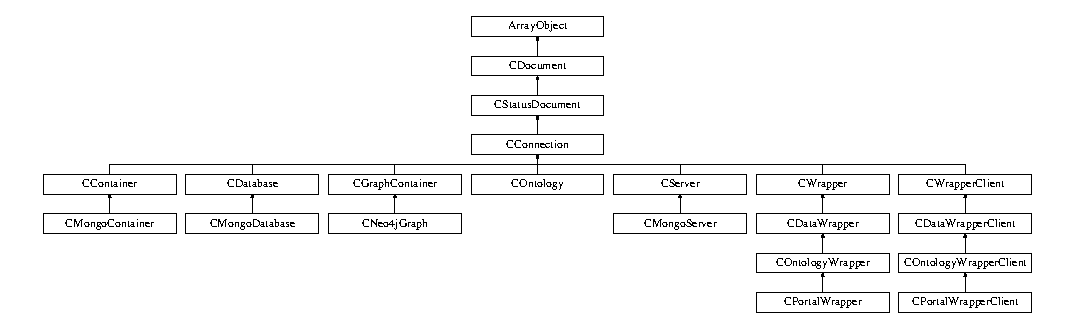
\includegraphics[height=3.975155cm]{class_c_connection}
\end{center}
\end{figure}
\subsection*{Public Member Functions}
\begin{DoxyCompactItemize}
\item 
\hyperlink{class_c_connection_a5214faf06b04e39885b00e6181991e68}{\-\_\-\-\_\-construct} (\$the\-Connection=N\-U\-L\-L, \$the\-Options=N\-U\-L\-L)
\item 
\hyperlink{class_c_connection_af23aaa67a594e82ff0c43287dc205925}{\-\_\-\-\_\-to\-String} ()
\item 
\hyperlink{class_c_connection_a8ad981138c7b681c875da778ce4e391b}{Connection} (\$the\-Value=N\-U\-L\-L, \$get\-Old=F\-A\-L\-S\-E)
\end{DoxyCompactItemize}
\subsection*{Protected Member Functions}
\begin{DoxyCompactItemize}
\item 
\hyperlink{class_c_connection_a173b6438388d14a21a74c7bbe265958b}{\-\_\-\-Ready} ()
\end{DoxyCompactItemize}
\subsection*{Protected Attributes}
\begin{DoxyCompactItemize}
\item 
\hypertarget{class_c_connection_a97443cb1bba958489af619a23f92b9cd}{{\bfseries \$m\-Connection} = N\-U\-L\-L}\label{class_c_connection_a97443cb1bba958489af619a23f92b9cd}

\end{DoxyCompactItemize}


\subsection{Constructor \& Destructor Documentation}
\hypertarget{class_c_connection_a5214faf06b04e39885b00e6181991e68}{\index{C\-Connection@{C\-Connection}!\-\_\-\-\_\-construct@{\-\_\-\-\_\-construct}}
\index{\-\_\-\-\_\-construct@{\-\_\-\-\_\-construct}!CConnection@{C\-Connection}}
\subsubsection[{\-\_\-\-\_\-construct}]{\setlength{\rightskip}{0pt plus 5cm}C\-Connection\-::\-\_\-\-\_\-construct (
\begin{DoxyParamCaption}
\item[{}]{\$the\-Connection = {\ttfamily NULL}, }
\item[{}]{\$the\-Options = {\ttfamily NULL}}
\end{DoxyParamCaption}
)}}\label{class_c_connection_a5214faf06b04e39885b00e6181991e68}
\subparagraph*{Instantiate class}

You instantiate the class with a native connection, the method expects a parameter that will be stored in the \hyperlink{}{\$m\-Connection} data member and another parameter that can be used to pass instantiation options.

Derived classes should overload this method if a default value is possible; to check for specific connection types they should rather overload the member accessor method.


\begin{DoxyParams}[1]{Parameters}
mixed & {\em \$the\-Connection} & Native connection. \\
\hline
mixed & {\em \$the\-Options} & Connection options.\\
\hline
\end{DoxyParams}
public

\hyperlink{class_c_connection_a8ad981138c7b681c875da778ce4e391b}{Connection()} 

\subsection{Member Function Documentation}
\hypertarget{class_c_connection_af23aaa67a594e82ff0c43287dc205925}{\index{C\-Connection@{C\-Connection}!\-\_\-\-\_\-to\-String@{\-\_\-\-\_\-to\-String}}
\index{\-\_\-\-\_\-to\-String@{\-\_\-\-\_\-to\-String}!CConnection@{C\-Connection}}
\subsubsection[{\-\_\-\-\_\-to\-String}]{\setlength{\rightskip}{0pt plus 5cm}C\-Connection\-::\-\_\-\-\_\-to\-String (
\begin{DoxyParamCaption}
{}
\end{DoxyParamCaption}
)\hspace{0.3cm}{\ttfamily [abstract]}}}\label{class_c_connection_af23aaa67a594e82ff0c43287dc205925}
\subparagraph*{Return connection name}

This method should return the current connection's name.

All derived concrete classes should implement this method, all connections must be able to return a name.

public \begin{DoxyReturn}{Returns}
string The connection name. 
\end{DoxyReturn}
\hypertarget{class_c_connection_a173b6438388d14a21a74c7bbe265958b}{\index{C\-Connection@{C\-Connection}!\-\_\-\-Ready@{\-\_\-\-Ready}}
\index{\-\_\-\-Ready@{\-\_\-\-Ready}!CConnection@{C\-Connection}}
\subsubsection[{\-\_\-\-Ready}]{\setlength{\rightskip}{0pt plus 5cm}C\-Connection\-::\-\_\-\-Ready (
\begin{DoxyParamCaption}
{}
\end{DoxyParamCaption}
)\hspace{0.3cm}{\ttfamily [protected]}}}\label{class_c_connection_a173b6438388d14a21a74c7bbe265958b}
\subparagraph*{Determine if the object is ready}

In this class we tie the \hyperlink{class_c_status_document_a954dee06e219e0a0f2e7fa6edac56e28}{\-\_\-\-Is\-Inited()} status to the presence or absence of the connection.

protected \begin{DoxyReturn}{Returns}
boolean {\ttfamily T\-R\-U\-E} means \hyperlink{}{.  \-\_\-\-Ready() }
\end{DoxyReturn}
\hypertarget{class_c_connection_a8ad981138c7b681c875da778ce4e391b}{\index{C\-Connection@{C\-Connection}!Connection@{Connection}}
\index{Connection@{Connection}!CConnection@{C\-Connection}}
\subsubsection[{Connection}]{\setlength{\rightskip}{0pt plus 5cm}C\-Connection\-::\-Connection (
\begin{DoxyParamCaption}
\item[{}]{\$the\-Value = {\ttfamily NULL}, }
\item[{}]{\$get\-Old = {\ttfamily FALSE}}
\end{DoxyParamCaption}
)}}\label{class_c_connection_a8ad981138c7b681c875da778ce4e391b}
\subparagraph*{Manage native connection}

This method can be used to manage the connection, it accepts a parameter which represents either the container or the requested operation, depending on its value\-:


\begin{DoxyItemize}
\item {\ttfamily N\-U\-L\-L}\-: Return the current value. 
\item {\ttfamily F\-A\-L\-S\-E}\-: Delete the current value. 
\item {\itshape other}\-: Set the value with the provided parameter. 
\end{DoxyItemize}

The second parameter is a boolean which if {\ttfamily T\-R\-U\-E} will return the {\itshape old} value when replacing containers; if {\ttfamily F\-A\-L\-S\-E}, it will return the currently set value.

In derived classes you should overload this method to check if the provided connection is of the correct type, in this class we accept anything.

This class is considered initialised (\hyperlink{class_c_status_document_a954dee06e219e0a0f2e7fa6edac56e28}{\-\_\-\-Is\-Inited()}) when this member has been set.


\begin{DoxyParams}[1]{Parameters}
mixed & {\em \$the\-Value} & Native connection or operation. \\
\hline
boolean & {\em \$get\-Old} & {\ttfamily T\-R\-U\-E} get old value.\\
\hline
\end{DoxyParams}
public \begin{DoxyReturn}{Returns}
mixed {\itshape New} or {\itshape old} native connection.
\end{DoxyReturn}
\-\_\-is\-Inited()  Manage\-Property() 

The documentation for this class was generated from the following file\-:\begin{DoxyCompactItemize}
\item 
/\-Library/\-Web\-Server/\-Library/\-P\-H\-P\-Wrapper/classes/C\-Connection.\-php\end{DoxyCompactItemize}

\hypertarget{class_c_container}{\section{C\-Container Class Reference}
\label{class_c_container}\index{C\-Container@{C\-Container}}
}
Inheritance diagram for C\-Container\-:\begin{figure}[H]
\begin{center}
\leavevmode
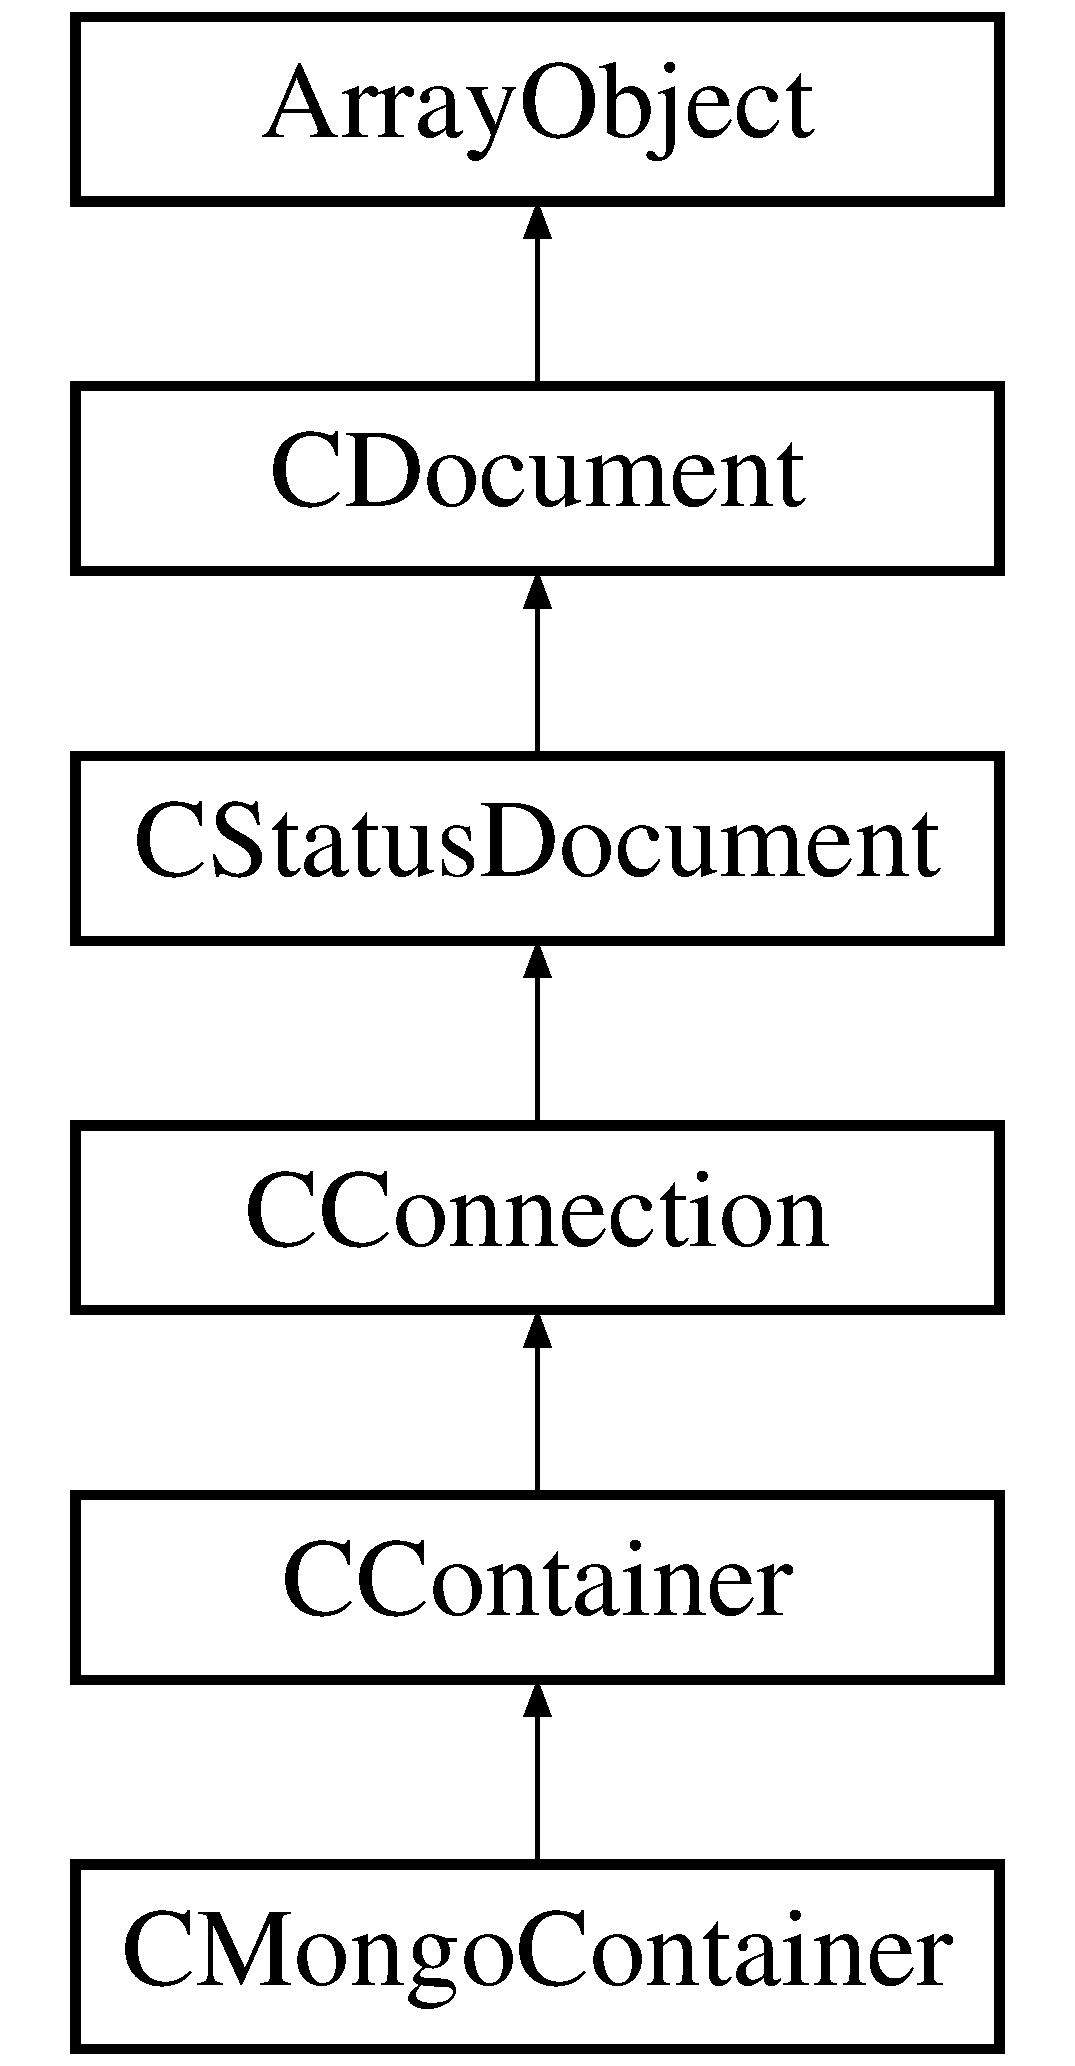
\includegraphics[height=6.000000cm]{class_c_container}
\end{center}
\end{figure}
\subsection*{Public Member Functions}
\begin{DoxyCompactItemize}
\item 
\hyperlink{class_c_container_acc336649ca3737a5870ca808a735101c}{\-\_\-\-\_\-destruct} ()
\item 
\hyperlink{class_c_container_ae896641925887415d2b364fadc894904}{Drop} ()
\item 
\hyperlink{class_c_container_ade4cbaf7d8aecd823a5b2342ebe9a79f}{Add\-Index} (\$the\-Index, \$the\-Options=Array())
\item 
\hyperlink{class_c_container_ae2a912b433ba916ce5af0b21d657243b}{Manage\-Object} (\&\$the\-Object, \$the\-Identifier=N\-U\-L\-L, \$the\-Modifiers=k\-F\-L\-A\-G\-\_\-\-D\-E\-F\-A\-U\-L\-T)
\item 
\hyperlink{class_c_container_abbb981df971e40d73bc530209c184028}{Check\-Object} (\$the\-Identifier, \$the\-Offset=N\-U\-L\-L)
\item 
\hyperlink{class_c_container_a9f422d5c6d99eea28993614749ee05a3}{Query} (\$the\-Query=N\-U\-L\-L, \$the\-Fields=N\-U\-L\-L, \$the\-Sort=N\-U\-L\-L, \$the\-Start=N\-U\-L\-L, \$the\-Limit=N\-U\-L\-L, \$the\-Result=N\-U\-L\-L)
\item 
\hyperlink{class_c_container_a1deac33bfa698889c45d9021a274392a}{Remove} (\$the\-Query=N\-U\-L\-L)
\item 
\hyperlink{class_c_container_aa339d3c4c9b011713176a89fe9c7783d}{Unserialise\-Object} (\&\$the\-Object)
\item 
\hyperlink{class_c_container_a02b227658d1799d3608973312f67b28c}{Unserialise\-Data} (\&\$the\-Element, \$the\-Type=N\-U\-L\-L)
\item 
\hyperlink{class_c_container_afa72f0da28ad8c3955cb9fedbc0ac2df}{Next\-Sequence} (\$the\-Key, \$the\-Container=N\-U\-L\-L)
\end{DoxyCompactItemize}
\subsection*{Static Public Member Functions}
\begin{DoxyCompactItemize}
\item 
static \hyperlink{class_c_container_af564e0d279b21cd89069ff8622ce2bc7}{New\-Query} (\$the\-Query=N\-U\-L\-L)
\end{DoxyCompactItemize}
\subsection*{Additional Inherited Members}


\subsection{Constructor \& Destructor Documentation}
\hypertarget{class_c_container_acc336649ca3737a5870ca808a735101c}{\index{C\-Container@{C\-Container}!\-\_\-\-\_\-destruct@{\-\_\-\-\_\-destruct}}
\index{\-\_\-\-\_\-destruct@{\-\_\-\-\_\-destruct}!CContainer@{C\-Container}}
\subsubsection[{\-\_\-\-\_\-destruct}]{\setlength{\rightskip}{0pt plus 5cm}C\-Container\-::\-\_\-\-\_\-destruct (
\begin{DoxyParamCaption}
{}
\end{DoxyParamCaption}
)}}\label{class_c_container_acc336649ca3737a5870ca808a735101c}
\subparagraph*{Destructor}

We implement the destructor to get rid of the graph\-: the Neo4j P\-H\-P interface, for instance, has closures that cannot be serialised, so we need to reset the graph \hyperlink{}{k\-O\-F\-F\-S\-E\-T\-\_\-\-G\-R\-A\-P\-H} offset before destroying the object.

public 

\subsection{Member Function Documentation}
\hypertarget{class_c_container_ade4cbaf7d8aecd823a5b2342ebe9a79f}{\index{C\-Container@{C\-Container}!Add\-Index@{Add\-Index}}
\index{Add\-Index@{Add\-Index}!CContainer@{C\-Container}}
\subsubsection[{Add\-Index}]{\setlength{\rightskip}{0pt plus 5cm}C\-Container\-::\-Add\-Index (
\begin{DoxyParamCaption}
\item[{}]{\$the\-Index, }
\item[{}]{\$the\-Options = {\ttfamily Array()}}
\end{DoxyParamCaption}
)\hspace{0.3cm}{\ttfamily [abstract]}}}\label{class_c_container_ade4cbaf7d8aecd823a5b2342ebe9a79f}
\subparagraph*{Add an index}

This method should be implemented by derived concrete instances.


\begin{DoxyParams}[1]{Parameters}
array & {\em \$the\-Index} & Key/\-Sort list. \\
\hline
array & {\em \$the\-Options} & List of index options.\\
\hline
\end{DoxyParams}
public \hypertarget{class_c_container_abbb981df971e40d73bc530209c184028}{\index{C\-Container@{C\-Container}!Check\-Object@{Check\-Object}}
\index{Check\-Object@{Check\-Object}!CContainer@{C\-Container}}
\subsubsection[{Check\-Object}]{\setlength{\rightskip}{0pt plus 5cm}C\-Container\-::\-Check\-Object (
\begin{DoxyParamCaption}
\item[{}]{\$the\-Identifier, }
\item[{}]{\$the\-Offset = {\ttfamily NULL}}
\end{DoxyParamCaption}
)\hspace{0.3cm}{\ttfamily [abstract]}}}\label{class_c_container_abbb981df971e40d73bc530209c184028}
\subparagraph*{Check if object exists in container}

This method can be used to check if an object exists in the current container, the method expects an identifier and an optional offset, it will return {\ttfamily T\-R\-U\-E} if found and {\ttfamily F\-A\-L\-S\-E} if not.


\begin{DoxyParams}[1]{Parameters}
mixed & {\em \$the\-Identifier} & Identifier. \\
\hline
string & {\em \$the\-Offset} & Offset.\\
\hline
\end{DoxyParams}
public \begin{DoxyReturn}{Returns}
boolean {\ttfamily T\-R\-U\-E} exists. 
\end{DoxyReturn}
\hypertarget{class_c_container_ae896641925887415d2b364fadc894904}{\index{C\-Container@{C\-Container}!Drop@{Drop}}
\index{Drop@{Drop}!CContainer@{C\-Container}}
\subsubsection[{Drop}]{\setlength{\rightskip}{0pt plus 5cm}C\-Container\-::\-Drop (
\begin{DoxyParamCaption}
{}
\end{DoxyParamCaption}
)\hspace{0.3cm}{\ttfamily [abstract]}}}\label{class_c_container_ae896641925887415d2b364fadc894904}
\subparagraph*{Delete a container}

This method should be implemented by derived concrete instances.

public \hypertarget{class_c_container_ae2a912b433ba916ce5af0b21d657243b}{\index{C\-Container@{C\-Container}!Manage\-Object@{Manage\-Object}}
\index{Manage\-Object@{Manage\-Object}!CContainer@{C\-Container}}
\subsubsection[{Manage\-Object}]{\setlength{\rightskip}{0pt plus 5cm}C\-Container\-::\-Manage\-Object (
\begin{DoxyParamCaption}
\item[{\&}]{\$the\-Object, }
\item[{}]{\$the\-Identifier = {\ttfamily NULL}, }
\item[{}]{\$the\-Modifiers = {\ttfamily kFLAG\-\_\-DEFAULT}}
\end{DoxyParamCaption}
)\hspace{0.3cm}{\ttfamily [abstract]}}}\label{class_c_container_ae2a912b433ba916ce5af0b21d657243b}
\subparagraph*{Manage an object from the container}

This method can be used to manage a single object in the container, it can {\itshape insert}, {\itshape update}, {\itshape replace}, {\itshape modify}, {\itshape retrieve} and {\itshape delete} an object from the current container by providing the object and/or its native unique identifier (\hyperlink{}{k\-T\-A\-G\-\_\-\-N\-I\-D}).

This method expects three parameters\-:


\begin{DoxyItemize}
\item {\ttfamily \$the\-Object}\-: The object or the data to be handled. 
\item {\ttfamily \$the\-Identifier}\-: The native unique identifier (\hyperlink{}{k\-T\-A\-G\-\_\-\-N\-I\-D}) of the object. If the value is {\itshape N\-U\-L\-L}, it means that it is the duty of the current container to set the value, this will generally be the case when inserting objects; in all other cases the parameter is required. 
\item {\ttfamily \$the\-Modifiers}\-: This parameter represents the operation options, or the list of offsets to be returned. If the parameter is not an array, it will be interpreted as a bitfield where the following values apply\-: 
\begin{DoxyItemize}
\item \hyperlink{}{k\-F\-L\-A\-G\-\_\-\-P\-E\-R\-S\-I\-S\-T\-\_\-\-I\-N\-S\-E\-R\-T}\-: The provided object will be inserted in the container. It is assumed that no other element in the container shares the same identifier, if not, the method should raise an exception. In this case the {\ttfamily \$the\-Object} represents the full object and {\ttfamily \$the\-Identifier} represents the object unique identifier, or {\ttfamily N\-U\-L\-L}, if it is the duty of the container to create the identifier. If the identifier was created by the container, it is the duty of this method to set it into the provided object. In this case the method should return the inserted object's native identifier (\hyperlink{}{k\-T\-A\-G\-\_\-\-N\-I\-D}). 
\item \hyperlink{}{k\-F\-L\-A\-G\-\_\-\-P\-E\-R\-S\-I\-S\-T\-\_\-\-U\-P\-D\-A\-T\-E}\-: The provided object will replace an object existing in the container. In this case the {\ttfamily \$the\-Object} represents the full object and {\ttfamily \$the\-Identifier} represents the object unique identifier. In this case the method should return {\ttfamily T\-R\-U\-E} if the object was updated and {\ttfamily F\-A\-L\-S\-E} if the object was not found. 
\item \hyperlink{}{k\-F\-L\-A\-G\-\_\-\-P\-E\-R\-S\-I\-S\-T\-\_\-\-R\-E\-P\-L\-A\-C\-E}\-: The provided object will be inserted if the identifier is missing or it doesn't match any entry in the container, or it will update the object corresponding to the provided identifier. This option represents the combination of the \hyperlink{}{k\-F\-L\-A\-G\-\_\-\-P\-E\-R\-S\-I\-S\-T\-\_\-\-I\-N\-S\-E\-R\-T} and \hyperlink{}{k\-F\-L\-A\-G\-\_\-\-P\-E\-R\-S\-I\-S\-T\-\_\-\-U\-P\-D\-A\-T\-E} operations. In this case the {\ttfamily \$the\-Object} represents the full object and {\ttfamily \$the\-Identifier} represents the object unique identifier, or {\ttfamily N\-U\-L\-L}, if it is the duty of the container to create the identifier. If the identifier was created by the container, it is the duty of this method to set it into the provided object. In this case the method should return the inserted object's native identifier (\hyperlink{}{k\-T\-A\-G\-\_\-\-N\-I\-D}). 
\item \hyperlink{}{k\-F\-L\-A\-G\-\_\-\-P\-E\-R\-S\-I\-S\-T\-\_\-\-M\-O\-D\-I\-F\-Y}\-: This option can be used to apply modifications to a subset of the object. In this case the parameters of this method have the following functions\-: 
\begin{DoxyItemize}
\item {\ttfamily \$the\-Object}\-: This parameter will be an array of elements whose {\itshape key} corresponds to the offset to be considered and the {\itshape value} to the value that the operation will use. 
\item {\ttfamily \$the\-Identifier}\-: This parameter keeps its original meaning, it should contain the native identifier of the object to be modified. If this parameter is a \hyperlink{class_c_query}{C\-Query} instance, this will be used to select the objects to be modified. 
\item {\ttfamily \$the\-Modifiers}\-: Another section of this bitfield will hold the flags that determine what specific modification should be performed\-: 
\begin{DoxyItemize}
\item \hyperlink{}{k\-F\-L\-A\-G\-\_\-\-M\-O\-D\-I\-F\-Y\-\_\-\-I\-N\-C\-R\-E\-M\-E\-N\-T}\-: This flag indicates an increment or decrement operation, the method will take the value corresponding to the offset in {\ttfamily \$the\-Object} parameter and add it to the object identified by {\ttfamily \$the\-Identifier} in the container. For instance, to increment by one the '{\ttfamily A}' offset of object {\ttfamily X}, you would pass the {\ttfamily array( 'A' =$>$ 1 )} in {\ttfamily \$the\-Object}, {\ttfamily X} in {\ttfamily \$the\-Identifier} and set the k\-F\-L\-A\-G\-\_\-\-M\-O\-D\-I\-F\-Y\-\_\-\-I\-N\-C\-R\-E\-M\-E\-N\-T flag; to decrement by two you would pass {\ttfamily array( 'A' =$>$ -\/2 )} in {\ttfamily \$the\-Object}, with all other parameters unchanged. If the offset does not exist, it will be initialised with the increment value. 
\item \hyperlink{}{k\-F\-L\-A\-G\-\_\-\-M\-O\-D\-I\-F\-Y\-\_\-\-A\-P\-P\-E\-N\-D}\-: This flag indicates that we want to append a value to an existing array, the method will take the value corresponding to the offset in {\ttfamily \$the\-Object} and append it to the offset in {\ttfamily \$the\-Object} for the object identified by {\ttfamily \$the\-Identifier} in the container. For instance, to append the value '{\ttfamily A}' to the array in offset '{\ttfamily F\-I\-E\-L\-D}' for object {\ttfamily X}, you would pass the {\ttfamily array( 'F\-I\-E\-L\-D' =$>$ 'A' )} in {\ttfamily \$the\-Object}, {\ttfamily X} in {\ttfamily \$the\-Identifier} and set the k\-F\-L\-A\-G\-\_\-\-M\-O\-D\-I\-F\-Y\-\_\-\-A\-P\-P\-E\-N\-D flag. If the field does not exist, it will be created with an array composed of the provided append value; if the field exists and its value is not an array, an exception should be raised. Note that if you provide an array as the value, the method will assume that you want to append the elements of the array as individual items; if you provide an {\ttfamily Array\-Object}, instead, the method will assume you want to append the whole array as a single item. 
\item \hyperlink{}{k\-F\-L\-A\-G\-\_\-\-M\-O\-D\-I\-F\-Y\-\_\-\-A\-D\-D\-S\-E\-T}\-: This flag indicates that we want to add a value to a set, this operation is equivalent to \hyperlink{}{k\-F\-L\-A\-G\-\_\-\-M\-O\-D\-I\-F\-Y\-\_\-\-A\-P\-P\-E\-N\-D}, except that the value will be appended only if it doesn't exist already in the receiving array. 
\item \hyperlink{}{k\-F\-L\-A\-G\-\_\-\-M\-O\-D\-I\-F\-Y\-\_\-\-P\-O\-P}\-: This flag indicates that we want to remove the first or last element from an array. The method will take the value corresponding to the offset in {\ttfamily \$the\-Object} and check its sign\-: if positive, the method will remove the first element; if negative it will remove the last. For instance, to remove the first element in the '{\ttfamily F\-I\-E\-L\-D}' offset of object {\ttfamily X}, you would pass the {\ttfamily array( 'F\-I\-E\-L\-D' =$>$ 1 )} in {\ttfamily \$the\-Object}, {\ttfamily X} in {\ttfamily \$the\-Identifier} and set the k\-F\-L\-A\-G\-\_\-\-M\-O\-D\-I\-F\-Y\-\_\-\-P\-O\-P flag in {\ttfamily \$the\-Modifiers}; to remove the last element you would pass {\ttfamily array( 'F\-I\-E\-L\-D' =$>$ -\/1 )} in {\ttfamily \$the\-Object}. If the offset does not exist, the method should not fail; if the offset is not an array, the method should raise an exception. 
\item \hyperlink{}{k\-F\-L\-A\-G\-\_\-\-M\-O\-D\-I\-F\-Y\-\_\-\-P\-U\-L\-L}\-: This flag indicates that we want to remove all occurrences of a value from an array. For instance, to remove all occurrances of '{\ttfamily A}' from the array contained in the '{\ttfamily F\-I\-E\-L\-D}' offset of object {\ttfamily X}, you would pass {\ttfamily array( 'F\-I\-E\-L\-D' =$>$ 'A' )} in {\ttfamily \$the\-Object}, {\ttfamily X} in {\ttfamily \$the\-Identifier} and set the k\-F\-L\-A\-G\-\_\-\-M\-O\-D\-I\-F\-Y\-\_\-\-P\-U\-L\-L flag in {\ttfamily \$the\-Modifiers}. If the field exists and its value is not an array, an exception should be raised. 
\item \hyperlink{}{k\-F\-L\-A\-G\-\_\-\-M\-O\-D\-I\-F\-Y\-\_\-\-M\-A\-S\-K} {\itshape off}\-: If none of the above flags are set, it means that the key/value pairs set in {\ttfamily \$the\-Object} represent offsets to be added or removed, depending on the value part of the pair\-: if the value is {\ttfamily N\-U\-L\-L}, it means that you want to remove the offset; any other value will replace the existing offset or be added to the object. 
\end{DoxyItemize}
\end{DoxyItemize}In this case the method will return the modified object in the {\ttfamily \$the\-Object} parameter, or raise an exception if the operation fails. 
\item \hyperlink{}{k\-F\-L\-A\-G\-\_\-\-P\-E\-R\-S\-I\-S\-T\-\_\-\-D\-E\-L\-E\-T\-E}\-: This option assumes you want to remove the object from the container. In this case the {\ttfamily \$the\-Object} represents the full object and {\ttfamily \$the\-Identifier} represents the object unique identifier, what counts is that the object's unique identifier (\hyperlink{}{k\-T\-A\-G\-\_\-\-N\-I\-D}) is provided. If the object is not found in the container, the method should not fail. In this case the method should return {\ttfamily T\-R\-U\-E} if the object was deleted and {\ttfamily F\-A\-L\-S\-E} if the object was not found. 
\end{DoxyItemize}If none of the above flags are set, it means that the caller wants to retrieve the object identified by the \hyperlink{}{k\-T\-A\-G\-\_\-\-N\-I\-D} offset from the provided object or from the provided identifier. If found, the provided object will receive the located object and the method will return {\ttfamily T\-R\-U\-E}; if not found, the method will set the provided object to {\ttfamily N\-U\-L\-L} and return {\ttfamily F\-A\-L\-S\-E}. If the parameter is an array, it implies that the requested operation is to retrieve the object, the array will be interpreted as the list of object offsets to be returned, the \hyperlink{}{k\-T\-A\-G\-\_\-\-N\-I\-D} offset is returned by default. 
\end{DoxyItemize}

The method should raise an exception if the operation was not successful and update the provided object with whatever data the operation will generate.

The method will also raise an exception if the object is not yet initialised (\hyperlink{class_c_status_document_a954dee06e219e0a0f2e7fa6edac56e28}{\-\_\-\-Is\-Inited()}), this happens when the object received the native container.

This class is abstract, which means that derived classes must implement the specific functionality of specialised data stores, for this reason this method is declared abstract.


\begin{DoxyParams}[1]{Parameters}
reference & {\em \&\$the\-Object} & Object. \\
\hline
mixed & {\em \$the\-Identifier} & Identifier. \\
\hline
mixed & {\em \$the\-Modifiers} & Options or offsets list.\\
\hline
\end{DoxyParams}
public \begin{DoxyReturn}{Returns}
mixed The native operation status.
\end{DoxyReturn}
\begin{DoxySeeAlso}{See Also}
k\-F\-L\-A\-G\-\_\-\-P\-E\-R\-S\-I\-S\-T\-\_\-\-I\-N\-S\-E\-R\-T k\-F\-L\-A\-G\-\_\-\-P\-E\-R\-S\-I\-S\-T\-\_\-\-U\-P\-D\-A\-T\-E k\-F\-L\-A\-G\-\_\-\-P\-E\-R\-S\-I\-S\-T\-\_\-\-M\-O\-D\-I\-F\-Y 

k\-F\-L\-A\-G\-\_\-\-P\-E\-R\-S\-I\-S\-T\-\_\-\-R\-E\-P\-L\-A\-C\-E k\-F\-L\-A\-G\-\_\-\-P\-E\-R\-S\-I\-S\-T\-\_\-\-M\-O\-D\-I\-F\-Y k\-F\-L\-A\-G\-\_\-\-P\-E\-R\-S\-I\-S\-T\-\_\-\-D\-E\-L\-E\-T\-E 

k\-F\-L\-A\-G\-\_\-\-M\-O\-D\-I\-F\-Y\-\_\-\-I\-N\-C\-R\-E\-M\-E\-N\-T k\-F\-L\-A\-G\-\_\-\-M\-O\-D\-I\-F\-Y\-\_\-\-A\-P\-P\-E\-N\-D k\-F\-L\-A\-G\-\_\-\-M\-O\-D\-I\-F\-Y\-\_\-\-A\-D\-D\-S\-E\-T 

k\-F\-L\-A\-G\-\_\-\-M\-O\-D\-I\-F\-Y\-\_\-\-P\-O\-P k\-F\-L\-A\-G\-\_\-\-M\-O\-D\-I\-F\-Y\-\_\-\-P\-U\-L\-L k\-F\-L\-A\-G\-\_\-\-M\-O\-D\-I\-F\-Y\-\_\-\-M\-A\-S\-K 
\end{DoxySeeAlso}
\hypertarget{class_c_container_af564e0d279b21cd89069ff8622ce2bc7}{\index{C\-Container@{C\-Container}!New\-Query@{New\-Query}}
\index{New\-Query@{New\-Query}!CContainer@{C\-Container}}
\subsubsection[{New\-Query}]{\setlength{\rightskip}{0pt plus 5cm}static C\-Container\-::\-New\-Query (
\begin{DoxyParamCaption}
\item[{}]{\$the\-Query = {\ttfamily NULL}}
\end{DoxyParamCaption}
)\hspace{0.3cm}{\ttfamily [static]}}}\label{class_c_container_af564e0d279b21cd89069ff8622ce2bc7}
\subparagraph*{Return an empty query}

This method can be used to retrieve an empty query, the main utility of this method is to return a query object that is compatible with the current container.

In this class we return an instance of the base \hyperlink{class_c_query}{C\-Query} class.


\begin{DoxyParams}[1]{Parameters}
mixed & {\em \$the\-Query} & Query data.\\
\hline
\end{DoxyParams}
\begin{DoxyReturn}{Returns}
\hyperlink{class_c_query}{C\-Query} An empty query object. 
\end{DoxyReturn}
\hypertarget{class_c_container_afa72f0da28ad8c3955cb9fedbc0ac2df}{\index{C\-Container@{C\-Container}!Next\-Sequence@{Next\-Sequence}}
\index{Next\-Sequence@{Next\-Sequence}!CContainer@{C\-Container}}
\subsubsection[{Next\-Sequence}]{\setlength{\rightskip}{0pt plus 5cm}C\-Container\-::\-Next\-Sequence (
\begin{DoxyParamCaption}
\item[{}]{\$the\-Key, }
\item[{}]{\$the\-Container = {\ttfamily NULL}}
\end{DoxyParamCaption}
)}}\label{class_c_container_afa72f0da28ad8c3955cb9fedbc0ac2df}
\subparagraph*{Return a sequence number}

This method should return a sequence number connected to the provided key. Each time this method is called, the sequence number is incremented, which means that you should only call it when you intend to use this number.

The first parameter, {\ttfamily \$the\-Key}, represents the key to the sequence, it will be the \hyperlink{}{k\-T\-A\-G\-\_\-\-N\-I\-D} of the record holding the sequence and the field holding the current number has the \hyperlink{}{k\-O\-F\-F\-S\-E\-T\-\_\-\-S\-E\-Q\-U\-E\-N\-C\-E} offset.

The second parameter represents the container in which the sequence is stored\-:


\begin{DoxyItemize}
\item {\ttfamily string{\ttfamily \-: The method should use the native container corresponding to the provided string. }}
\item {\ttfamily {\ttfamily {\ttfamily T\-R\-U\-E{\ttfamily \-: The method should use the string stored in \hyperlink{}{k\-C\-O\-N\-T\-A\-I\-N\-E\-R\-\_\-\-S\-E\-Q\-U\-E\-N\-C\-E\-\_\-\-N\-A\-M\-E}. }}}}
\item {\ttfamily {\ttfamily {\ttfamily {\ttfamily {\ttfamily N\-U\-L\-L{\ttfamily \-: The method should use the current container. }}}}}}
\end{DoxyItemize}

{\ttfamily {\ttfamily {\ttfamily {\ttfamily {\ttfamily {\ttfamily If the object is not \hyperlink{}{Inited()}, the method should raise an exception.}}}}}}

{\ttfamily {\ttfamily {\ttfamily {\ttfamily {\ttfamily {\ttfamily If the current object does not support sequences, this method should return {\ttfamily N\-U\-L\-L}.}}}}}}

{\ttfamily {\ttfamily {\ttfamily {\ttfamily {\ttfamily {\ttfamily This class is abstract and by default sequences are not supported.}}}}}}

{\ttfamily {\ttfamily {\ttfamily {\ttfamily {\ttfamily {\ttfamily 
\begin{DoxyParams}[1]{Parameters}
string & {\em \$the\-Key} & Sequence key. \\
\hline
mixed & {\em \$the\-Container} & Sequence container.\\
\hline
\end{DoxyParams}
public \begin{DoxyReturn}{Returns}
mixed The sequence number or {\ttfamily N\-U\-L\-L}.
\end{DoxyReturn}

\begin{DoxyExceptions}{Exceptions}
{\em Exception} & \\
\hline
\end{DoxyExceptions}
}}}}}}\hypertarget{class_c_container_a9f422d5c6d99eea28993614749ee05a3}{\index{C\-Container@{C\-Container}!Query@{Query}}
\index{Query@{Query}!CContainer@{C\-Container}}
\subsubsection[{Query}]{\setlength{\rightskip}{0pt plus 5cm}C\-Container\-::\-Query (
\begin{DoxyParamCaption}
\item[{}]{\$the\-Query = {\ttfamily NULL}, }
\item[{}]{\$the\-Fields = {\ttfamily NULL}, }
\item[{}]{\$the\-Sort = {\ttfamily NULL}, }
\item[{}]{\$the\-Start = {\ttfamily NULL}, }
\item[{}]{\$the\-Limit = {\ttfamily NULL}, }
\item[{}]{\$the\-Result = {\ttfamily NULL}}
\end{DoxyParamCaption}
)\hspace{0.3cm}{\ttfamily [abstract]}}}\label{class_c_container_a9f422d5c6d99eea28993614749ee05a3}
\subparagraph*{Perform a query}

This method can be used to perform a query on the container, it expects an instance of \hyperlink{class_c_query}{C\-Query} as the query, or {\ttfamily N\-U\-L\-L}, to query the whole container and two optional parameters that represents the list of desired fields and the list of sort fields with sense.


\begin{DoxyItemize}
\item {\ttfamily \$the\-Query}\-: The query expressed as an array or query object, if omitted, it is assumed the query should cover the whole contents of the container. 
\item {\ttfamily \$the\-Fields}\-: The list of fields to be returned, if omitted, it is assumed all fields are to be returned. 
\item {\ttfamily \$the\-Sort}\-: The query sort order provided as an array in which the key represents the field name and he value a number that represents the sense\-: negative numbers indicate descending order and positive numbers ascending order; a value of zero will be skipped. 
\item {\ttfamily \$the\-Start}\-: The record number on which to start returning results (zero based). 
\item {\ttfamily \$the\-Limit}\-: The maximum number of records to be returned. 
\item {\ttfamily \$the\-Result}\-: This parameter determines the result of the method\-: 
\begin{DoxyItemize}
\item {\ttfamily N\-U\-L\-L}\-: Return the selection cursor (default). 
\item {\ttfamily T\-R\-U\-E}\-: Return first matched record or {\ttfamily N\-U\-L\-L} if there were no matches. 
\item {\itshape other}\-: Any other value will be interpreted as a field identifier\-: in this case the method will return an array containing the distinct values of the provided field identifier. 
\end{DoxyItemize}
\end{DoxyItemize}

When {\ttfamily \$the\-Result} is set to {\ttfamily N\-U\-L\-L}, the method should return an object that represents a cursor into the query results, the object should be iterable and feature a method, {\itshape count}, that accepts a boolean parameter\-: if {\ttfamily T\-R\-U\-E} the method should return the actual number of elements available taking into consideration paging parameters; if {\ttfamily F\-A\-L\-S\-E}, the method should return the total affected elements count, that is, the total number of elements affected by the query regardless of paging parameters.


\begin{DoxyParams}[1]{Parameters}
array & {\em \$the\-Query} & Query. \\
\hline
array & {\em \$the\-Fields} & Fields set. \\
\hline
array & {\em \$the\-Sort} & Sort order. \\
\hline
integer & {\em \$the\-Start} & Page start. \\
\hline
integer & {\em \$the\-Limit} & Page limit. \\
\hline
mixed & {\em \$the\-Result} & Result type.\\
\hline
\end{DoxyParams}
public \begin{DoxyReturn}{Returns}
object Native recordset. 
\end{DoxyReturn}
\hypertarget{class_c_container_a1deac33bfa698889c45d9021a274392a}{\index{C\-Container@{C\-Container}!Remove@{Remove}}
\index{Remove@{Remove}!CContainer@{C\-Container}}
\subsubsection[{Remove}]{\setlength{\rightskip}{0pt plus 5cm}C\-Container\-::\-Remove (
\begin{DoxyParamCaption}
\item[{}]{\$the\-Query = {\ttfamily NULL}}
\end{DoxyParamCaption}
)\hspace{0.3cm}{\ttfamily [abstract]}}}\label{class_c_container_a1deac33bfa698889c45d9021a274392a}
\subparagraph*{Perform a deletion}

This method can be used to delete elements of a container, it expects an instance of \hyperlink{class_c_query}{C\-Query} as the query, or {\ttfamily N\-U\-L\-L}, to delete the whole container.


\begin{DoxyItemize}
\item {\ttfamily \$the\-Query}\-: The query expressed as an array or query object, if omitted, it is assumed the query should cover the whole contents of the container. 
\end{DoxyItemize}

If the query selected no object, the method should return {\ttfamily N\-U\-L\-L}, if the operation succeeded the method should return an integer containing the number of affected objects; on errors the method should raise an exception.


\begin{DoxyParams}[1]{Parameters}
array & {\em \$the\-Query} & Query.\\
\hline
\end{DoxyParams}
public \begin{DoxyReturn}{Returns}
integer Number of affected elements. 
\end{DoxyReturn}
\hypertarget{class_c_container_a02b227658d1799d3608973312f67b28c}{\index{C\-Container@{C\-Container}!Unserialise\-Data@{Unserialise\-Data}}
\index{Unserialise\-Data@{Unserialise\-Data}!CContainer@{C\-Container}}
\subsubsection[{Unserialise\-Data}]{\setlength{\rightskip}{0pt plus 5cm}C\-Container\-::\-Unserialise\-Data (
\begin{DoxyParamCaption}
\item[{\&}]{\$the\-Element, }
\item[{}]{\$the\-Type = {\ttfamily NULL}}
\end{DoxyParamCaption}
)\hspace{0.3cm}{\ttfamily [abstract]}}}\label{class_c_container_a02b227658d1799d3608973312f67b28c}
Unserialise provided data element.

This method should convert the provided structure into a custom data type compatible with the current container.

This method is called by a public \hyperlink{class_c_container_aa339d3c4c9b011713176a89fe9c7783d}{Unserialise\-Object()} interface which traverses an object and provides this method with all elements that satisfy the following conditions\-:


\begin{DoxyItemize}
\item {\ttfamily \hyperlink{class_c_data_type}{C\-Data\-Type}}\-: All instances derived from this class are sent to this method. 
\item {\ttfamily Array} or {\ttfamily Array\-Object}\-: If the structure is composed of exactly two offsets and these elements are \hyperlink{}{k\-T\-A\-G\-\_\-\-C\-U\-S\-T\-O\-M\-\_\-\-T\-Y\-P\-E} and \hyperlink{}{k\-T\-A\-G\-\_\-\-C\-U\-S\-T\-O\-M\-\_\-\-D\-A\-T\-A}, it will be sent to this method. 
\end{DoxyItemize}

The elements to be converted are provided by reference, which means that they have to be converted in place.

This method can also be used in a different way\-: you can ask the method to convert the provided scalar to the corresponding custom type, for this you need to provide a scalar in the first parameter and a data type in the second.

In this class we declare this class abstract, derived concrete classes must implement it.


\begin{DoxyParams}[1]{Parameters}
reference & {\em \&\$the\-Element} & Element to encode. \\
\hline
string & {\em \$the\-Type} & Data type.\\
\hline
\end{DoxyParams}
public \hypertarget{class_c_container_aa339d3c4c9b011713176a89fe9c7783d}{\index{C\-Container@{C\-Container}!Unserialise\-Object@{Unserialise\-Object}}
\index{Unserialise\-Object@{Unserialise\-Object}!CContainer@{C\-Container}}
\subsubsection[{Unserialise\-Object}]{\setlength{\rightskip}{0pt plus 5cm}C\-Container\-::\-Unserialise\-Object (
\begin{DoxyParamCaption}
\item[{\&}]{\$the\-Object}
\end{DoxyParamCaption}
)}}\label{class_c_container_aa339d3c4c9b011713176a89fe9c7783d}
Unserialise provided object.

This method will convert concrete derived instances of \hyperlink{class_c_data_type}{C\-Data\-Type} or equivalent structures into native data types suitable to be stored in containers.

This method will scan the provided object or structure and pass all instances derived from \hyperlink{class_c_data_type}{C\-Data\-Type} to another public \hyperlink{class_c_container_a02b227658d1799d3608973312f67b28c}{Unserialise\-Data()} method that will convert these objects into native data types that are compatible with the specific container type.

The method will scan the provided structure and select all elements which are arrays, Array\-Objects or objects derived from \hyperlink{class_c_data_type}{C\-Data\-Type}, these elements will be sent to the \hyperlink{class_c_container_a02b227658d1799d3608973312f67b28c}{Unserialise\-Data()} method that will take care of converting these structures into native data types that are compatible with the specific container type.

The method will perform the conversion directly into the provided reference and will use recursion to traverse the provided structures.

Elements sent to the \hyperlink{class_c_container_a02b227658d1799d3608973312f67b28c}{Unserialise\-Data()} method are selected as follows\-:


\begin{DoxyItemize}
\item {\ttfamily \hyperlink{class_c_data_type}{C\-Data\-Type}}\-: All instances derived from this class are sent to the \hyperlink{class_c_container_a02b227658d1799d3608973312f67b28c}{Unserialise\-Data()} method. 
\item {\ttfamily Array} or {\ttfamily Array\-Object}\-: If the structure is composed of exactly two offsets and these elements are \hyperlink{}{k\-T\-A\-G\-\_\-\-C\-U\-S\-T\-O\-M\-\_\-\-T\-Y\-P\-E} and \hyperlink{}{k\-T\-A\-G\-\_\-\-C\-U\-S\-T\-O\-M\-\_\-\-D\-A\-T\-A}, it will be sent to the \hyperlink{class_c_container_a02b227658d1799d3608973312f67b28c}{Unserialise\-Data()} method. If the above condition is not satisfied, the structure will be sent recursively to this method. 
\end{DoxyItemize}


\begin{DoxyParams}[1]{Parameters}
reference & {\em \&\$the\-Object} & Object to encode.\\
\hline
\end{DoxyParams}
public

\hyperlink{class_c_container_a02b227658d1799d3608973312f67b28c}{Unserialise\-Data()}

\begin{DoxySeeAlso}{See Also}
k\-T\-A\-G\-\_\-\-C\-U\-S\-T\-O\-M\-\_\-\-T\-Y\-P\-E k\-T\-A\-G\-\_\-\-C\-U\-S\-T\-O\-M\-\_\-\-D\-A\-T\-A 
\end{DoxySeeAlso}


The documentation for this class was generated from the following file\-:\begin{DoxyCompactItemize}
\item 
/\-Library/\-Web\-Server/\-Library/\-P\-H\-P\-Wrapper/classes/C\-Container.\-php\end{DoxyCompactItemize}

\hypertarget{class_c_database}{\section{C\-Database Class Reference}
\label{class_c_database}\index{C\-Database@{C\-Database}}
}
Inheritance diagram for C\-Database\-:\begin{figure}[H]
\begin{center}
\leavevmode
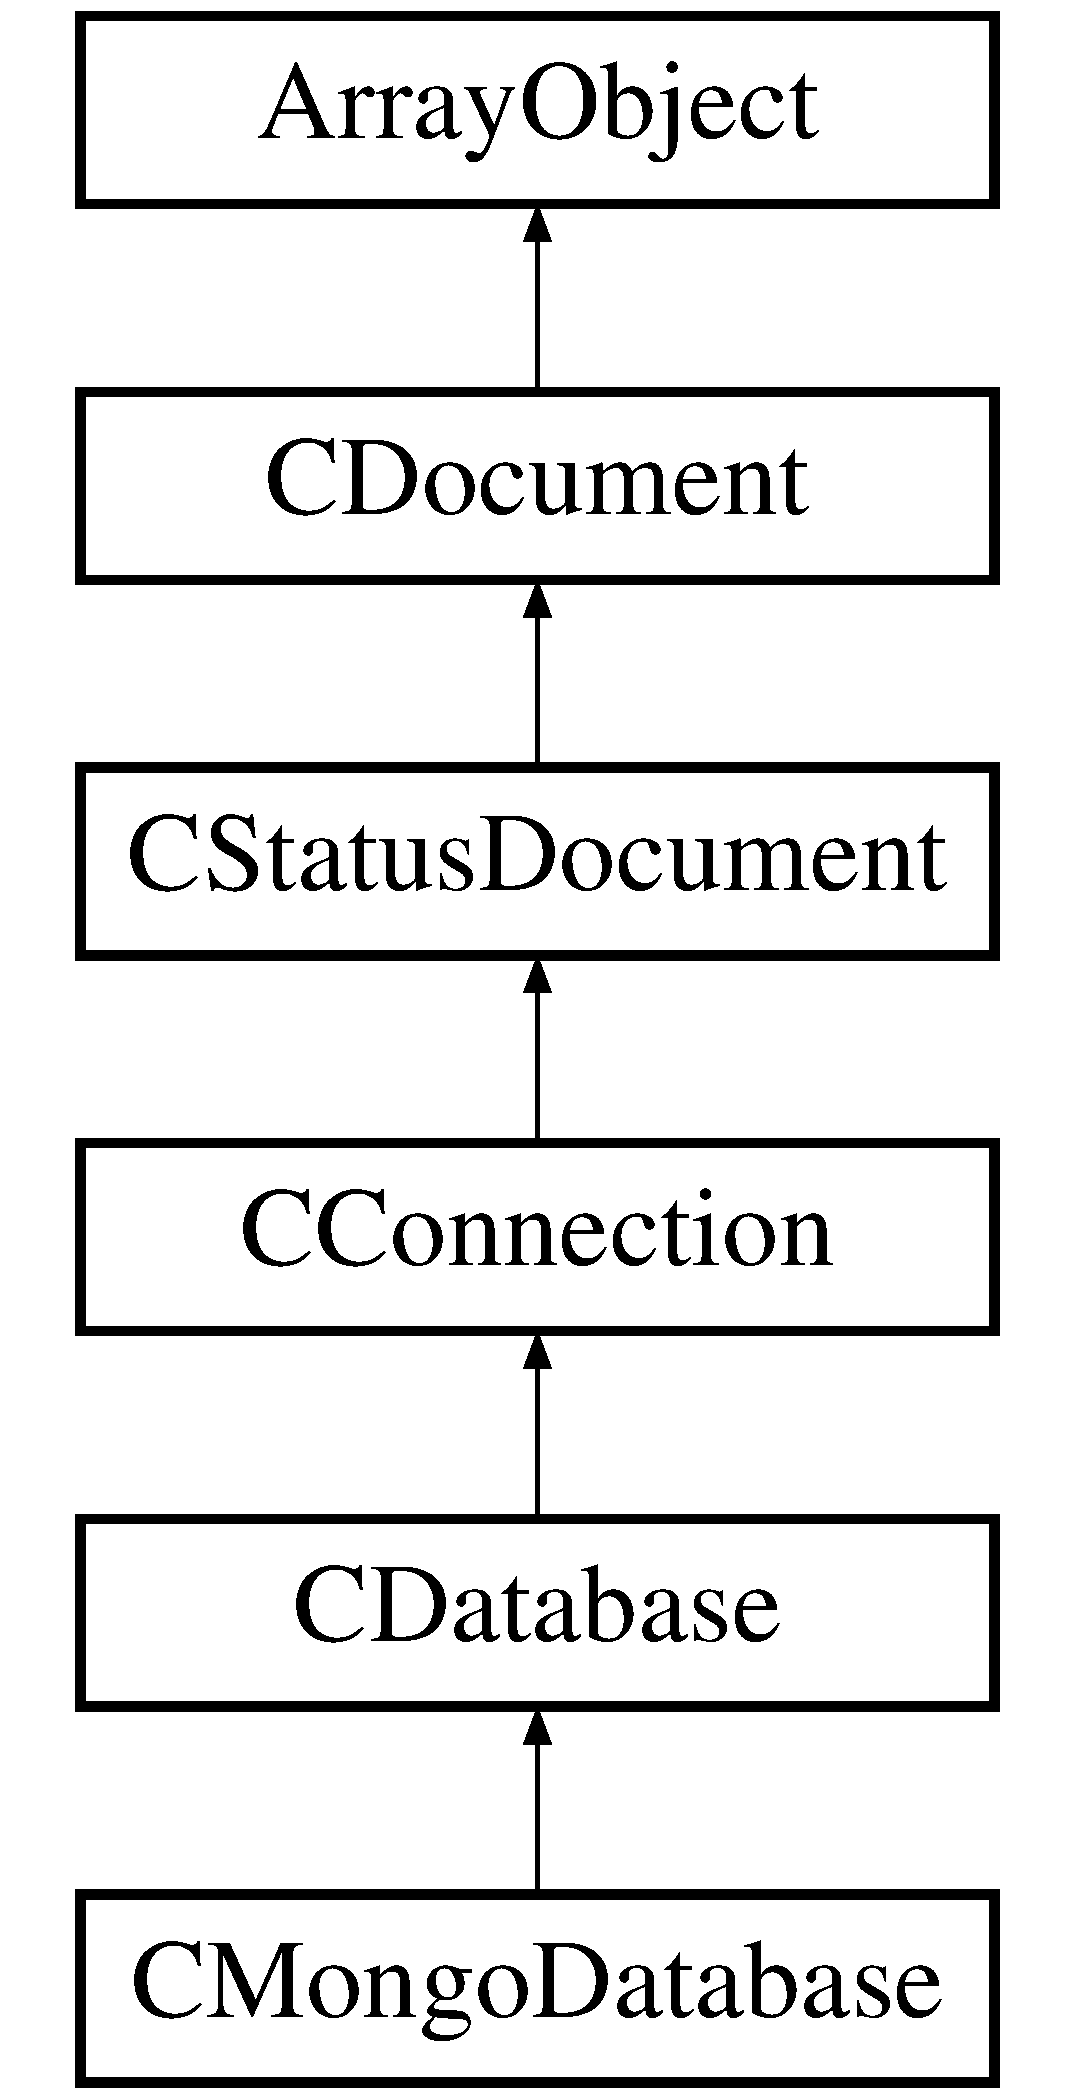
\includegraphics[height=6.000000cm]{class_c_database}
\end{center}
\end{figure}
\subsection*{Public Member Functions}
\begin{DoxyCompactItemize}
\item 
\hyperlink{class_c_database_a378c145a3e033c52205fb4ec5765247c}{\-\_\-\-\_\-destruct} ()
\item 
\hyperlink{class_c_database_a21dd7143f4a3bc8d8cbbfb24ced5970f}{Drop} ()
\item 
\hyperlink{class_c_database_a2e93bccc867d3eac9bca95abd74a2030}{Container} (\$the\-Container=N\-U\-L\-L)
\end{DoxyCompactItemize}
\subsection*{Additional Inherited Members}


\subsection{Constructor \& Destructor Documentation}
\hypertarget{class_c_database_a378c145a3e033c52205fb4ec5765247c}{\index{C\-Database@{C\-Database}!\-\_\-\-\_\-destruct@{\-\_\-\-\_\-destruct}}
\index{\-\_\-\-\_\-destruct@{\-\_\-\-\_\-destruct}!CDatabase@{C\-Database}}
\subsubsection[{\-\_\-\-\_\-destruct}]{\setlength{\rightskip}{0pt plus 5cm}C\-Database\-::\-\_\-\-\_\-destruct (
\begin{DoxyParamCaption}
{}
\end{DoxyParamCaption}
)}}\label{class_c_database_a378c145a3e033c52205fb4ec5765247c}
\subparagraph*{Destructor}

We implement the destructor to get rid of the graph\-: the Neo4j P\-H\-P interface, for instance, has closures that cannot be serialised, so we need to reset the graph \hyperlink{}{k\-O\-F\-F\-S\-E\-T\-\_\-\-G\-R\-A\-P\-H} offset before destroying the object.

public 

\subsection{Member Function Documentation}
\hypertarget{class_c_database_a2e93bccc867d3eac9bca95abd74a2030}{\index{C\-Database@{C\-Database}!Container@{Container}}
\index{Container@{Container}!CDatabase@{C\-Database}}
\subsubsection[{Container}]{\setlength{\rightskip}{0pt plus 5cm}C\-Database\-::\-Container (
\begin{DoxyParamCaption}
\item[{}]{\$the\-Container = {\ttfamily NULL}}
\end{DoxyParamCaption}
)\hspace{0.3cm}{\ttfamily [abstract]}}}\label{class_c_database_a2e93bccc867d3eac9bca95abd74a2030}
\subparagraph*{Generate a container object}

This method can be used to return a container object belonging to the current database.

The parameter will be used by concrete instances to select which container to return, the goal of this class is only to declare the public interface, which must be implemented by specialised derived classes.

{\itshape Note\-: This method should also take care of setting the \hyperlink{}{k\-O\-F\-F\-S\-E\-T\-\_\-\-N\-A\-M\-E}, \hyperlink{}{k\-O\-F\-F\-S\-E\-T\-\_\-\-G\-R\-A\-P\-H} and \hyperlink{}{k\-O\-F\-F\-S\-E\-T\-\_\-\-P\-A\-R\-E\-N\-T} offsets of the generated object.}


\begin{DoxyParams}[1]{Parameters}
mixed & {\em \$the\-Container} & Container selector.\\
\hline
\end{DoxyParams}
public \begin{DoxyReturn}{Returns}
mixed The container object.
\end{DoxyReturn}
\begin{DoxySeeAlso}{See Also}
k\-O\-F\-F\-S\-E\-T\-\_\-\-N\-A\-M\-E k\-O\-F\-F\-S\-E\-T\-\_\-\-G\-R\-A\-P\-H k\-O\-F\-F\-S\-E\-T\-\_\-\-P\-A\-R\-E\-N\-T 
\end{DoxySeeAlso}
\hypertarget{class_c_database_a21dd7143f4a3bc8d8cbbfb24ced5970f}{\index{C\-Database@{C\-Database}!Drop@{Drop}}
\index{Drop@{Drop}!CDatabase@{C\-Database}}
\subsubsection[{Drop}]{\setlength{\rightskip}{0pt plus 5cm}C\-Database\-::\-Drop (
\begin{DoxyParamCaption}
{}
\end{DoxyParamCaption}
)\hspace{0.3cm}{\ttfamily [abstract]}}}\label{class_c_database_a21dd7143f4a3bc8d8cbbfb24ced5970f}
\subparagraph*{Delete a database}

This method can be used to delete or erase a database, it is up to derived concrete instances to implement it.

The method takes no parameters.

public 

The documentation for this class was generated from the following file\-:\begin{DoxyCompactItemize}
\item 
/\-Library/\-Web\-Server/\-Library/\-P\-H\-P\-Wrapper/classes/C\-Database.\-php\end{DoxyCompactItemize}

\hypertarget{class_c_data_type}{\section{C\-Data\-Type Class Reference}
\label{class_c_data_type}\index{C\-Data\-Type@{C\-Data\-Type}}
}
Inheritance diagram for C\-Data\-Type\-:\begin{figure}[H]
\begin{center}
\leavevmode
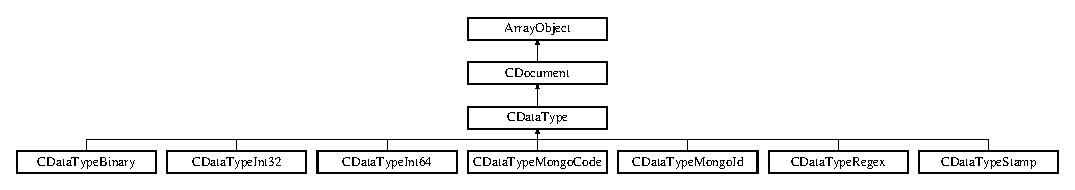
\includegraphics[height=2.105263cm]{class_c_data_type}
\end{center}
\end{figure}
\subsection*{Public Member Functions}
\begin{DoxyCompactItemize}
\item 
\hyperlink{class_c_data_type_a52f7a2ebe5e01eed9995115a410d83ab}{\-\_\-\-\_\-construct} (\$the\-Data=N\-U\-L\-L)
\item 
\hyperlink{class_c_data_type_a47c70c056d328f35497a6e712bf9be1c}{\-\_\-\-\_\-to\-String} ()
\item 
\hyperlink{class_c_data_type_a6f013843044529b54c2df535fc1471a8}{value} ()
\end{DoxyCompactItemize}
\subsection*{Static Public Member Functions}
\begin{DoxyCompactItemize}
\item 
static \hyperlink{class_c_data_type_a608d6fc184bce537ce83669f729d6008}{Serialise\-Object} (\&\$the\-Object)
\item 
static \hyperlink{class_c_data_type_ae15089a7237ed4e95279b398f44f8f47}{Serialise\-Element} (\&\$the\-Element, \&\$the\-Type)
\item 
static \hyperlink{class_c_data_type_a1cae522eec386d293b6087a99e9a8b0b}{Serialise\-Data} (\&\$the\-Element)
\end{DoxyCompactItemize}


\subsection{Constructor \& Destructor Documentation}
\hypertarget{class_c_data_type_a52f7a2ebe5e01eed9995115a410d83ab}{\index{C\-Data\-Type@{C\-Data\-Type}!\-\_\-\-\_\-construct@{\-\_\-\-\_\-construct}}
\index{\-\_\-\-\_\-construct@{\-\_\-\-\_\-construct}!CDataType@{C\-Data\-Type}}
\subsubsection[{\-\_\-\-\_\-construct}]{\setlength{\rightskip}{0pt plus 5cm}C\-Data\-Type\-::\-\_\-\-\_\-construct (
\begin{DoxyParamCaption}
\item[{}]{\$the\-Data = {\ttfamily NULL}}
\end{DoxyParamCaption}
)}}\label{class_c_data_type_a52f7a2ebe5e01eed9995115a410d83ab}
Instantiate class.

This class enforces a standard constructor that accepts one parameter which represents the custom data contents, these will be stored in the \hyperlink{}{k\-T\-A\-G\-\_\-\-C\-U\-S\-T\-O\-M\-\_\-\-D\-A\-T\-A} offset, this element must be filled.

The method will ensure that this parameter is not {\ttfamily N\-U\-L\-L} and not an array; it may be an Array\-Object, but it must then have the \-\_\-to\-String() method.

No {\ttfamily N\-U\-L\-L} concrete instance is allowed, all instances derived from this class must have a value.

The \hyperlink{}{\} offset will be set by derived classes.  mixed \$the\-Data Custom data.  public }

\subsection{Member Function Documentation}
\hypertarget{class_c_data_type_a47c70c056d328f35497a6e712bf9be1c}{\index{C\-Data\-Type@{C\-Data\-Type}!\-\_\-\-\_\-to\-String@{\-\_\-\-\_\-to\-String}}
\index{\-\_\-\-\_\-to\-String@{\-\_\-\-\_\-to\-String}!CDataType@{C\-Data\-Type}}
\subsubsection[{\-\_\-\-\_\-to\-String}]{\setlength{\rightskip}{0pt plus 5cm}C\-Data\-Type\-::\-\_\-\-\_\-to\-String (
\begin{DoxyParamCaption}
{}
\end{DoxyParamCaption}
)}}\label{class_c_data_type_a47c70c056d328f35497a6e712bf9be1c}
Return string representation.

This method should return a string representation of the custom data type contents, this method must be implemented for all concrete classes.

By default this method expects the custom data part to be convertable to string, if this is not the case, overload this method.

public \begin{DoxyReturn}{Returns}
string 
\end{DoxyReturn}
\hypertarget{class_c_data_type_a1cae522eec386d293b6087a99e9a8b0b}{\index{C\-Data\-Type@{C\-Data\-Type}!Serialise\-Data@{Serialise\-Data}}
\index{Serialise\-Data@{Serialise\-Data}!CDataType@{C\-Data\-Type}}
\subsubsection[{Serialise\-Data}]{\setlength{\rightskip}{0pt plus 5cm}static C\-Data\-Type\-::\-Serialise\-Data (
\begin{DoxyParamCaption}
\item[{\&}]{\$the\-Element}
\end{DoxyParamCaption}
)\hspace{0.3cm}{\ttfamily [static]}}}\label{class_c_data_type_a1cae522eec386d293b6087a99e9a8b0b}
Serialise provided data element.

This method can be used to convert custom data types to a standard format that can be serialised and transmitted through the network. This method is generally called by \hyperlink{class_c_data_type_a608d6fc184bce537ce83669f729d6008}{Serialise\-Object()} which passes each scalar element as a reference to this method which should decide whether the provided element is to be converted or not.

This method will check if the provided parameter corresponds to a custom data type that needs to be converted, if so, it will convert it to an instance derived from this class.

The following data types will be converted\-:


\begin{DoxyItemize}
\item {\itshape Mongo\-Id}\-: We convert into a \hyperlink{class_c_data_type_mongo_id}{C\-Data\-Type\-Mongo\-Id} object. 
\item {\itshape Mongo\-Code}\-: We convert into a \hyperlink{class_c_data_type_mongo_code}{C\-Data\-Type\-Mongo\-Code} object. 
\item {\itshape Mongo\-Date}\-: We convert into a \hyperlink{class_c_data_type_stamp}{C\-Data\-Type\-Stamp} object. 
\item {\itshape Mongo\-Regex}\-: We convert into a \hyperlink{class_c_data_type_regex}{C\-Data\-Type\-Regex} object. 
\item {\itshape Mongo\-Bin\-Data}\-: We convert into a \hyperlink{class_c_data_type_binary}{C\-Data\-Type\-Binary} object. 
\item {\itshape Mongo\-Int32}\-: We convert into a \hyperlink{class_c_data_type_int32}{C\-Data\-Type\-Int32} object. 
\item {\itshape Mongo\-Int64}\-: We convert into a \hyperlink{class_c_data_type_int64}{C\-Data\-Type\-Int64} object. 
\end{DoxyItemize}


\begin{DoxyParams}[1]{Parameters}
reference & {\em \&\$the\-Element} & Element to encode. \\
\hline
\end{DoxyParams}
\hypertarget{class_c_data_type_ae15089a7237ed4e95279b398f44f8f47}{\index{C\-Data\-Type@{C\-Data\-Type}!Serialise\-Element@{Serialise\-Element}}
\index{Serialise\-Element@{Serialise\-Element}!CDataType@{C\-Data\-Type}}
\subsubsection[{Serialise\-Element}]{\setlength{\rightskip}{0pt plus 5cm}static C\-Data\-Type\-::\-Serialise\-Element (
\begin{DoxyParamCaption}
\item[{\&}]{\$the\-Element, }
\item[{\&}]{\$the\-Type}
\end{DoxyParamCaption}
)\hspace{0.3cm}{\ttfamily [static]}}}\label{class_c_data_type_ae15089a7237ed4e95279b398f44f8f47}
Serialise provided element.

This method can be used to enforce converting custom data types to a standard format that can be serialised and transmitted through the network. This method accepts two parameters\-: the data type and the value\-: depending on their combination, the method will convert in place the data and the type.


\begin{DoxyParams}[1]{Parameters}
reference & {\em \&\$the\-Element} & Element to encode. \\
\hline
string & {\em \&\$the\-Type} & Element data type.\\
\hline
\end{DoxyParams}

\begin{DoxyExceptions}{Exceptions}
{\em \hyperlink{class_c_exception}{C\-Exception}} & \\
\hline
\end{DoxyExceptions}
\hypertarget{class_c_data_type_a608d6fc184bce537ce83669f729d6008}{\index{C\-Data\-Type@{C\-Data\-Type}!Serialise\-Object@{Serialise\-Object}}
\index{Serialise\-Object@{Serialise\-Object}!CDataType@{C\-Data\-Type}}
\subsubsection[{Serialise\-Object}]{\setlength{\rightskip}{0pt plus 5cm}static C\-Data\-Type\-::\-Serialise\-Object (
\begin{DoxyParamCaption}
\item[{\&}]{\$the\-Object}
\end{DoxyParamCaption}
)\hspace{0.3cm}{\ttfamily [static]}}}\label{class_c_data_type_a608d6fc184bce537ce83669f729d6008}
Serialise provided object.

This method will take an object and convert all data elements that are compatible with one of the concrete classes derived from this one into a derived concrete instance.

This method is useful when encoding objects in a format suitable for being transmitted over the internet.

This method will ensure that the object contains data types compatible with P\-H\-P and this library; it will be the duty of persistent containers to convert these structures into custom data types compatible with their storage engines.

The method will scan the provided data elements\-: array or Array\-Object elements will be recursed, scalar elements will be sent to the public \hyperlink{class_c_data_type_a1cae522eec386d293b6087a99e9a8b0b}{Serialise\-Data()} method that will take care of performing the actual data conversion.

If an element of the provided structure is converted, it will {\itshape always} be an object derived from this class, and all conversions will be performed on the object itself, which means that you should expect the provided object to be modified.


\begin{DoxyParams}[1]{Parameters}
reference & {\em \&\$the\-Object} & Object to decode. \\
\hline
\end{DoxyParams}
\hypertarget{class_c_data_type_a6f013843044529b54c2df535fc1471a8}{\index{C\-Data\-Type@{C\-Data\-Type}!value@{value}}
\index{value@{value}!CDataType@{C\-Data\-Type}}
\subsubsection[{value}]{\setlength{\rightskip}{0pt plus 5cm}C\-Data\-Type\-::value (
\begin{DoxyParamCaption}
{}
\end{DoxyParamCaption}
)}}\label{class_c_data_type_a6f013843044529b54c2df535fc1471a8}
Return data value.

This method should return the custom data value in the closest type possible in P\-H\-P.

By default we return the string representation of the data, this is the last resort if the actual data type cannot be represented in P\-H\-P; derived classes that can be represented in P\-H\-P should overload this method.

public \begin{DoxyReturn}{Returns}
mixed
\end{DoxyReturn}

\begin{DoxyExceptions}{Exceptions}
{\em Exception} & \\
\hline
\end{DoxyExceptions}


The documentation for this class was generated from the following file\-:\begin{DoxyCompactItemize}
\item 
/\-Library/\-Web\-Server/\-Library/\-P\-H\-P\-Wrapper/classes/C\-Data\-Type.\-php\end{DoxyCompactItemize}

\hypertarget{class_c_data_type_binary}{\section{C\-Data\-Type\-Binary Class Reference}
\label{class_c_data_type_binary}\index{C\-Data\-Type\-Binary@{C\-Data\-Type\-Binary}}
}
Inheritance diagram for C\-Data\-Type\-Binary\-:\begin{figure}[H]
\begin{center}
\leavevmode
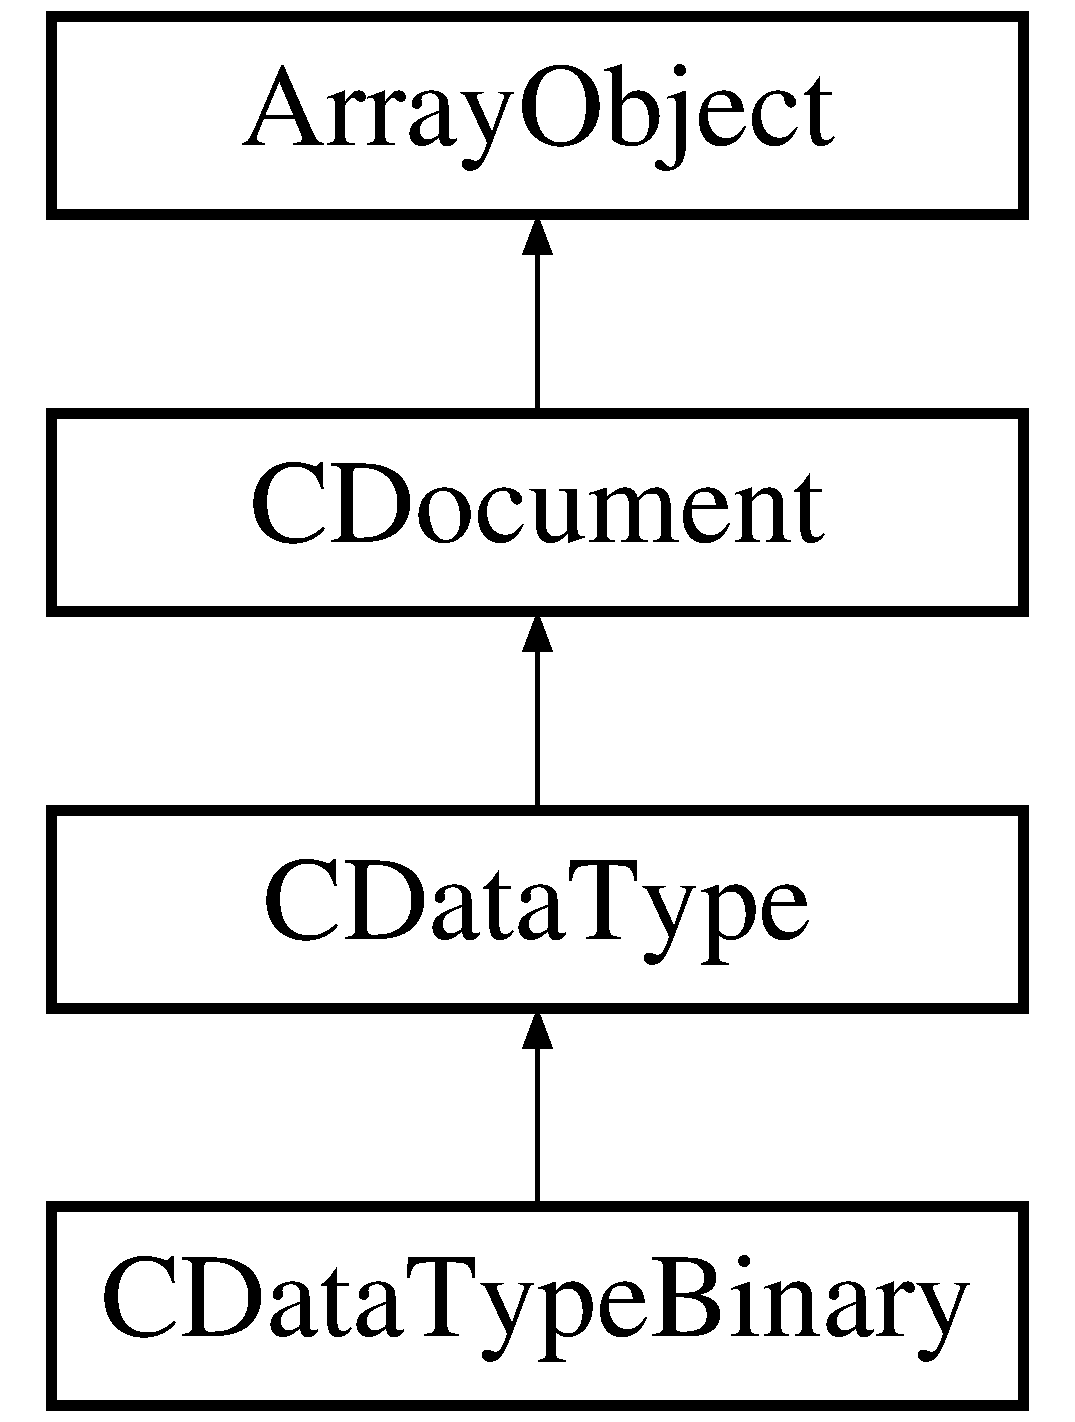
\includegraphics[height=4.000000cm]{class_c_data_type_binary}
\end{center}
\end{figure}
\subsection*{Public Member Functions}
\begin{DoxyCompactItemize}
\item 
\hyperlink{class_c_data_type_binary_a59d483e75d2facb20e958394039f6bf2}{\-\_\-\-\_\-construct} (\$the\-Data=N\-U\-L\-L)
\item 
\hyperlink{class_c_data_type_binary_af2d723e4b5f85b3ecae701841ef27470}{value} ()
\end{DoxyCompactItemize}
\subsection*{Static Public Member Functions}
\begin{DoxyCompactItemize}
\item 
static \hyperlink{class_c_data_type_binary_a213a2e4c041262b4b5f24375d20ae8fe}{From\-Hex} (\$the\-Hex)
\end{DoxyCompactItemize}


\subsection{Constructor \& Destructor Documentation}
\hypertarget{class_c_data_type_binary_a59d483e75d2facb20e958394039f6bf2}{\index{C\-Data\-Type\-Binary@{C\-Data\-Type\-Binary}!\-\_\-\-\_\-construct@{\-\_\-\-\_\-construct}}
\index{\-\_\-\-\_\-construct@{\-\_\-\-\_\-construct}!CDataTypeBinary@{C\-Data\-Type\-Binary}}
\subsubsection[{\-\_\-\-\_\-construct}]{\setlength{\rightskip}{0pt plus 5cm}C\-Data\-Type\-Binary\-::\-\_\-\-\_\-construct (
\begin{DoxyParamCaption}
\item[{}]{\$the\-Data = {\ttfamily NULL}}
\end{DoxyParamCaption}
)}}\label{class_c_data_type_binary_a59d483e75d2facb20e958394039f6bf2}
Instantiate class.

We overload the parent constructor to set the default \hyperlink{}{k\-T\-Y\-P\-E\-\_\-\-B\-I\-N\-A\-R\-Y\-\_\-\-S\-T\-R\-I\-N\-G} and to set the binary string into the \hyperlink{}{k\-T\-A\-G\-\_\-\-C\-U\-S\-T\-O\-M\-\_\-\-D\-A\-T\-A} offset.


\begin{DoxyParams}[1]{Parameters}
mixed & {\em \$the\-Data} & Custom data.\\
\hline
\end{DoxyParams}
public


\begin{DoxyExceptions}{Exceptions}
{\em Exception} & \\
\hline
\end{DoxyExceptions}


\subsection{Member Function Documentation}
\hypertarget{class_c_data_type_binary_a213a2e4c041262b4b5f24375d20ae8fe}{\index{C\-Data\-Type\-Binary@{C\-Data\-Type\-Binary}!From\-Hex@{From\-Hex}}
\index{From\-Hex@{From\-Hex}!CDataTypeBinary@{C\-Data\-Type\-Binary}}
\subsubsection[{From\-Hex}]{\setlength{\rightskip}{0pt plus 5cm}static C\-Data\-Type\-Binary\-::\-From\-Hex (
\begin{DoxyParamCaption}
\item[{}]{\$the\-Hex}
\end{DoxyParamCaption}
)\hspace{0.3cm}{\ttfamily [static]}}}\label{class_c_data_type_binary_a213a2e4c041262b4b5f24375d20ae8fe}
Create from hex.

This method will return an object created from the provided hexadecimal value.


\begin{DoxyParams}[1]{Parameters}
string & {\em \$the\-Hex} & Binary hexadecimal value.\\
\hline
\end{DoxyParams}
\begin{DoxyReturn}{Returns}
\hyperlink{class_c_data_type_binary}{C\-Data\-Type\-Binary} 
\end{DoxyReturn}
\hypertarget{class_c_data_type_binary_af2d723e4b5f85b3ecae701841ef27470}{\index{C\-Data\-Type\-Binary@{C\-Data\-Type\-Binary}!value@{value}}
\index{value@{value}!CDataTypeBinary@{C\-Data\-Type\-Binary}}
\subsubsection[{value}]{\setlength{\rightskip}{0pt plus 5cm}C\-Data\-Type\-Binary\-::value (
\begin{DoxyParamCaption}
{}
\end{DoxyParamCaption}
)}}\label{class_c_data_type_binary_af2d723e4b5f85b3ecae701841ef27470}
Return data value.

This method will return the actual binary string.

public \begin{DoxyReturn}{Returns}
float
\end{DoxyReturn}

\begin{DoxyExceptions}{Exceptions}
{\em Exception} & \\
\hline
\end{DoxyExceptions}


The documentation for this class was generated from the following file\-:\begin{DoxyCompactItemize}
\item 
/\-Library/\-Web\-Server/\-Library/\-P\-H\-P\-Wrapper/classes/C\-Data\-Type\-Binary.\-php\end{DoxyCompactItemize}

\hypertarget{class_c_data_type_int32}{\section{C\-Data\-Type\-Int32 Class Reference}
\label{class_c_data_type_int32}\index{C\-Data\-Type\-Int32@{C\-Data\-Type\-Int32}}
}
Inheritance diagram for C\-Data\-Type\-Int32\-:\begin{figure}[H]
\begin{center}
\leavevmode
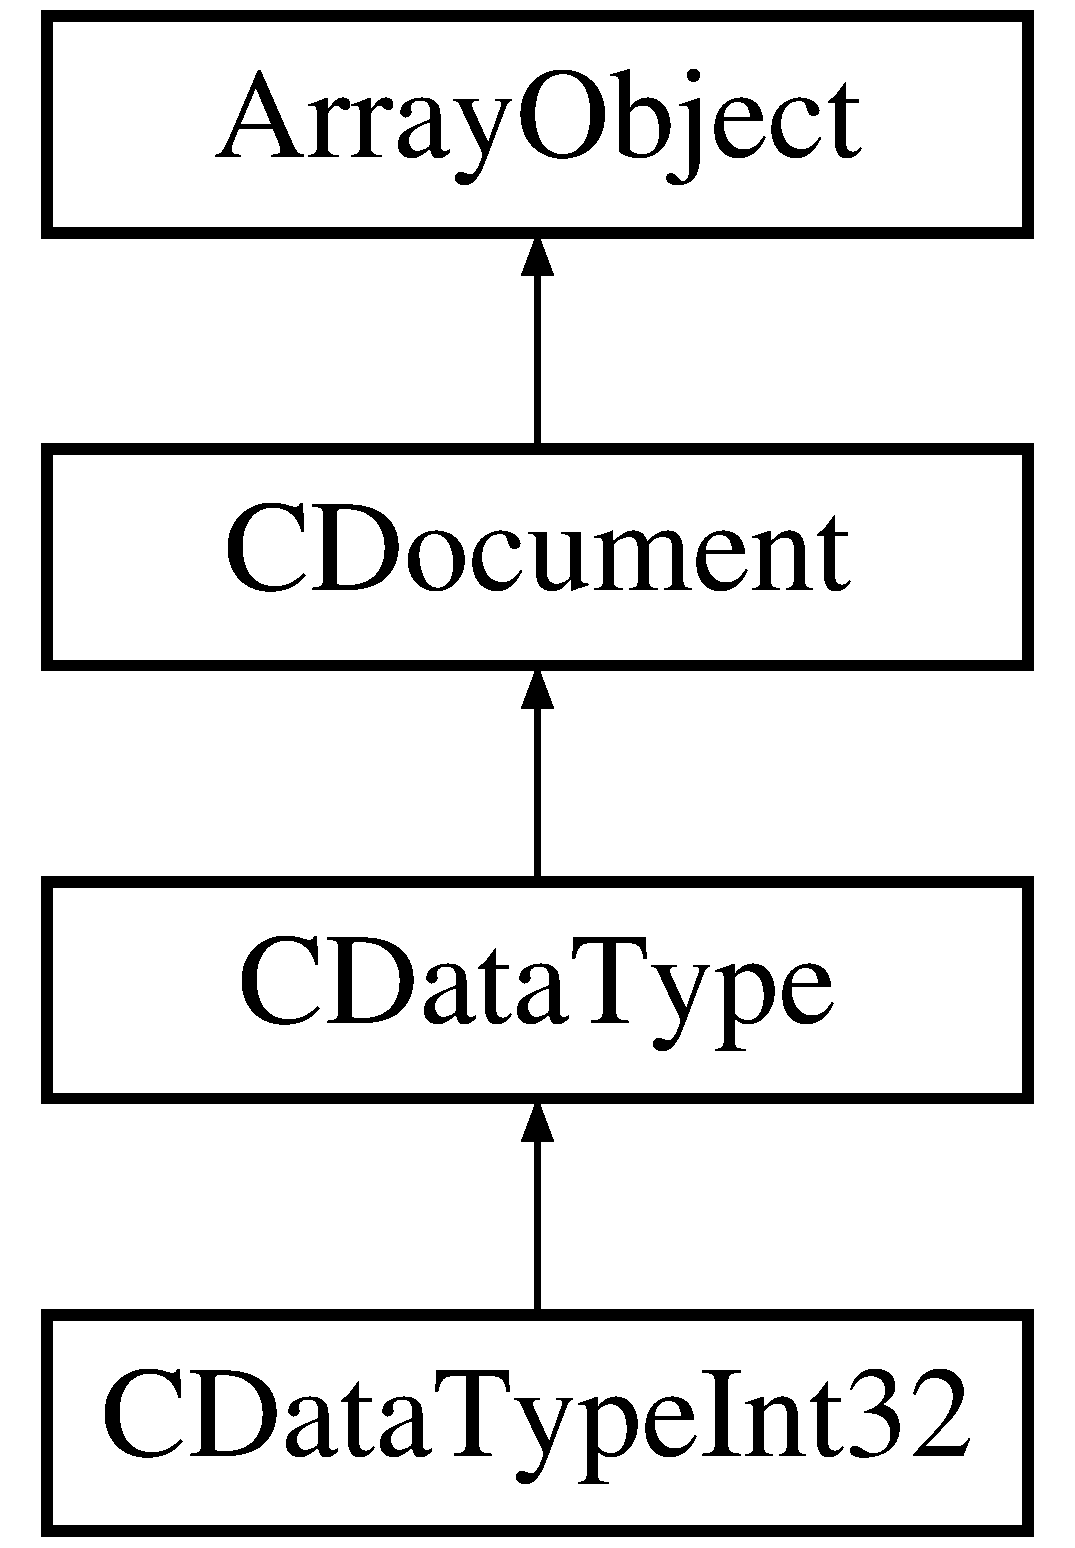
\includegraphics[height=4.000000cm]{class_c_data_type_int32}
\end{center}
\end{figure}
\subsection*{Public Member Functions}
\begin{DoxyCompactItemize}
\item 
\hyperlink{class_c_data_type_int32_a1181cc130ff3b0c573aeead09696b81f}{\-\_\-\-\_\-construct} (\$the\-Data=N\-U\-L\-L)
\item 
\hyperlink{class_c_data_type_int32_a5d95fb33639cb10a3cd54dde2b771f91}{value} ()
\end{DoxyCompactItemize}
\subsection*{Additional Inherited Members}


\subsection{Constructor \& Destructor Documentation}
\hypertarget{class_c_data_type_int32_a1181cc130ff3b0c573aeead09696b81f}{\index{C\-Data\-Type\-Int32@{C\-Data\-Type\-Int32}!\-\_\-\-\_\-construct@{\-\_\-\-\_\-construct}}
\index{\-\_\-\-\_\-construct@{\-\_\-\-\_\-construct}!CDataTypeInt32@{C\-Data\-Type\-Int32}}
\subsubsection[{\-\_\-\-\_\-construct}]{\setlength{\rightskip}{0pt plus 5cm}C\-Data\-Type\-Int32\-::\-\_\-\-\_\-construct (
\begin{DoxyParamCaption}
\item[{}]{\$the\-Data = {\ttfamily NULL}}
\end{DoxyParamCaption}
)}}\label{class_c_data_type_int32_a1181cc130ff3b0c573aeead09696b81f}
Instantiate class.

In this class we store \hyperlink{}{k\-T\-Y\-P\-E\-\_\-\-I\-N\-T32} in the \hyperlink{}{k\-T\-A\-G\-\_\-\-C\-U\-S\-T\-O\-M\-\_\-\-T\-Y\-P\-E} offset and the integer in the \hyperlink{}{k\-T\-A\-G\-\_\-\-C\-U\-S\-T\-O\-M\-\_\-\-D\-A\-T\-A} offset.

The method will check if the provided data (converted to string) is numeric, if this is not the case, it will raise an exception. This is to handle miscellaneous objects.


\begin{DoxyParams}[1]{Parameters}
mixed & {\em \$the\-Data} & Custom data.\\
\hline
\end{DoxyParams}
public


\begin{DoxyExceptions}{Exceptions}
{\em Exception} & \\
\hline
\end{DoxyExceptions}


\subsection{Member Function Documentation}
\hypertarget{class_c_data_type_int32_a5d95fb33639cb10a3cd54dde2b771f91}{\index{C\-Data\-Type\-Int32@{C\-Data\-Type\-Int32}!value@{value}}
\index{value@{value}!CDataTypeInt32@{C\-Data\-Type\-Int32}}
\subsubsection[{value}]{\setlength{\rightskip}{0pt plus 5cm}C\-Data\-Type\-Int32\-::value (
\begin{DoxyParamCaption}
{}
\end{DoxyParamCaption}
)}}\label{class_c_data_type_int32_a5d95fb33639cb10a3cd54dde2b771f91}
Return data value.

In this class we return the integer value, since P\-H\-P handles it.

public \begin{DoxyReturn}{Returns}
mixed
\end{DoxyReturn}

\begin{DoxyExceptions}{Exceptions}
{\em Exception} & \\
\hline
\end{DoxyExceptions}


The documentation for this class was generated from the following file\-:\begin{DoxyCompactItemize}
\item 
/\-Library/\-Web\-Server/\-Library/\-P\-H\-P\-Wrapper/classes/C\-Data\-Type\-Int32.\-php\end{DoxyCompactItemize}

\hypertarget{class_c_data_type_int64}{\section{C\-Data\-Type\-Int64 Class Reference}
\label{class_c_data_type_int64}\index{C\-Data\-Type\-Int64@{C\-Data\-Type\-Int64}}
}
Inheritance diagram for C\-Data\-Type\-Int64\-:\begin{figure}[H]
\begin{center}
\leavevmode
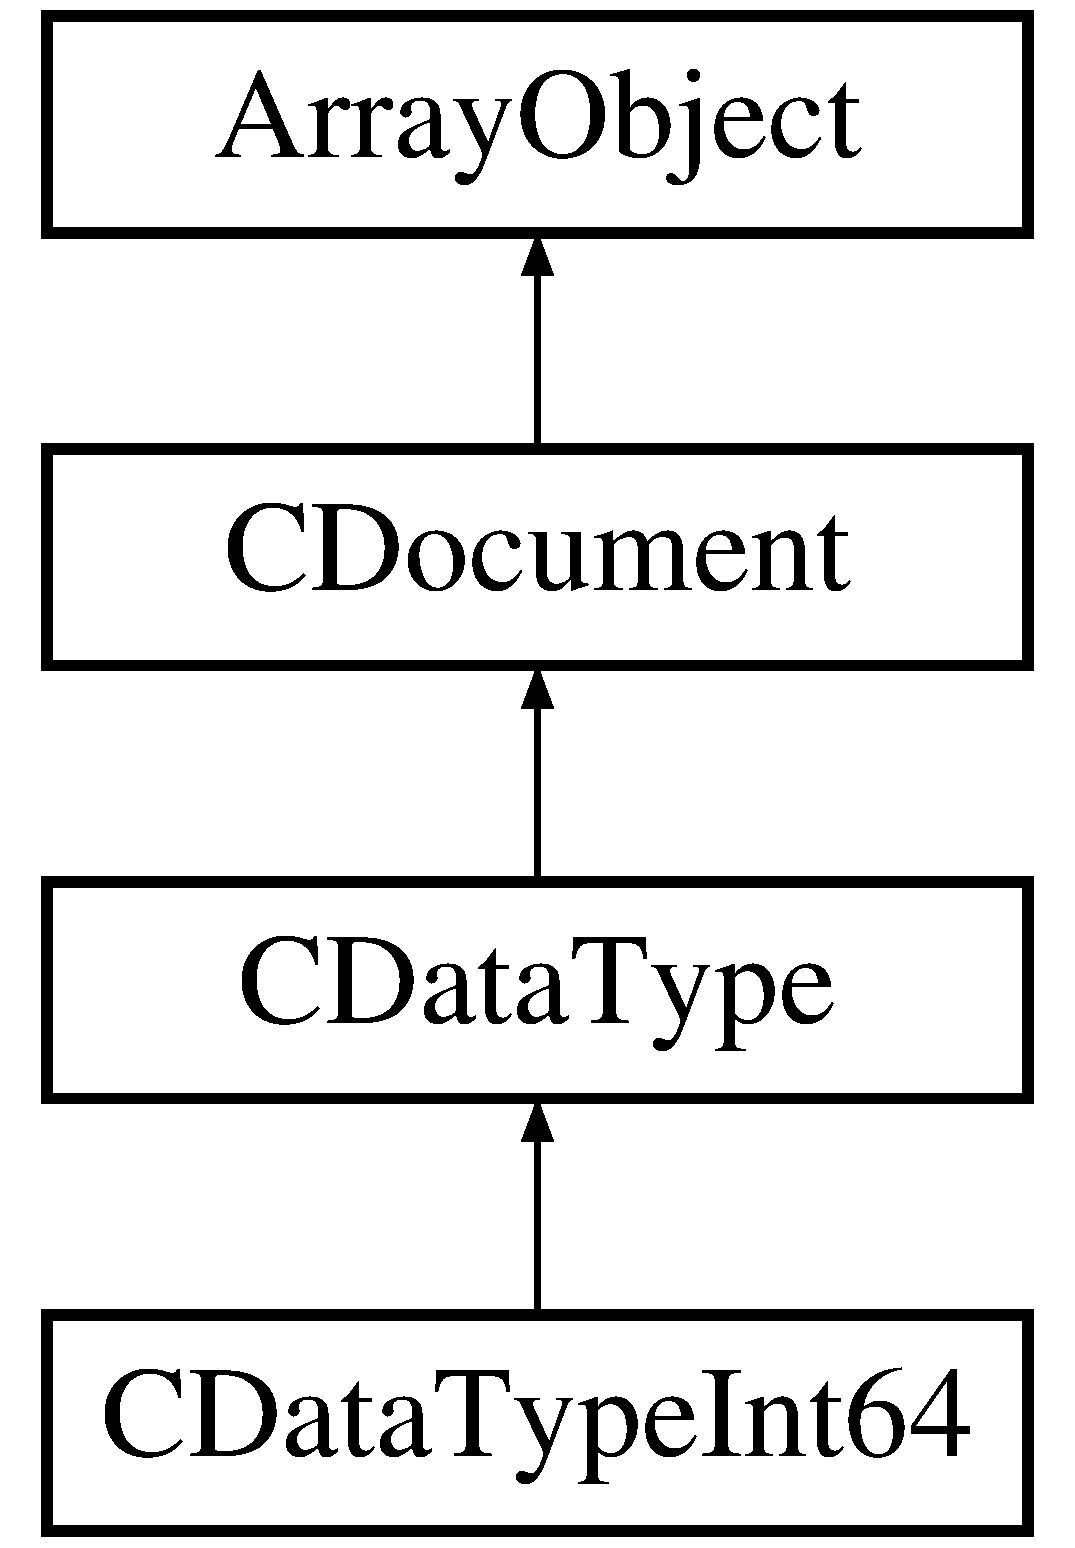
\includegraphics[height=4.000000cm]{class_c_data_type_int64}
\end{center}
\end{figure}
\subsection*{Public Member Functions}
\begin{DoxyCompactItemize}
\item 
\hyperlink{class_c_data_type_int64_ac628704dd037bbbc85601b4b111ea839}{\-\_\-\-\_\-construct} (\$the\-Data=N\-U\-L\-L)
\item 
\hyperlink{class_c_data_type_int64_a628aa7443dc28e2a6aaef982877d3559}{value} ()
\end{DoxyCompactItemize}
\subsection*{Additional Inherited Members}


\subsection{Constructor \& Destructor Documentation}
\hypertarget{class_c_data_type_int64_ac628704dd037bbbc85601b4b111ea839}{\index{C\-Data\-Type\-Int64@{C\-Data\-Type\-Int64}!\-\_\-\-\_\-construct@{\-\_\-\-\_\-construct}}
\index{\-\_\-\-\_\-construct@{\-\_\-\-\_\-construct}!CDataTypeInt64@{C\-Data\-Type\-Int64}}
\subsubsection[{\-\_\-\-\_\-construct}]{\setlength{\rightskip}{0pt plus 5cm}C\-Data\-Type\-Int64\-::\-\_\-\-\_\-construct (
\begin{DoxyParamCaption}
\item[{}]{\$the\-Data = {\ttfamily NULL}}
\end{DoxyParamCaption}
)}}\label{class_c_data_type_int64_ac628704dd037bbbc85601b4b111ea839}
Instantiate class.

In this class we store \hyperlink{}{k\-T\-Y\-P\-E\-\_\-\-I\-N\-T64} in the \hyperlink{}{k\-T\-A\-G\-\_\-\-C\-U\-S\-T\-O\-M\-\_\-\-T\-Y\-P\-E} offset and the integer in the \hyperlink{}{k\-T\-A\-G\-\_\-\-C\-U\-S\-T\-O\-M\-\_\-\-D\-A\-T\-A} offset.

The method will check if the provided data (converted to string) is numeric, if this is not the case, it will raise an exception. This is to handle miscellaneous objects.

The number will be stored in the \hyperlink{}{k\-T\-A\-G\-\_\-\-C\-U\-S\-T\-O\-M\-\_\-\-D\-A\-T\-A} offset as an integer, if the current system is 64 bits.


\begin{DoxyParams}[1]{Parameters}
mixed & {\em \$the\-Data} & Custom data.\\
\hline
\end{DoxyParams}
public


\begin{DoxyExceptions}{Exceptions}
{\em Exception} & \\
\hline
\end{DoxyExceptions}


\subsection{Member Function Documentation}
\hypertarget{class_c_data_type_int64_a628aa7443dc28e2a6aaef982877d3559}{\index{C\-Data\-Type\-Int64@{C\-Data\-Type\-Int64}!value@{value}}
\index{value@{value}!CDataTypeInt64@{C\-Data\-Type\-Int64}}
\subsubsection[{value}]{\setlength{\rightskip}{0pt plus 5cm}C\-Data\-Type\-Int64\-::value (
\begin{DoxyParamCaption}
{}
\end{DoxyParamCaption}
)}}\label{class_c_data_type_int64_a628aa7443dc28e2a6aaef982877d3559}
Return data value.

In this class we return the integer value, if P\-H\-P handles 8 byte integers, or we call the \hyperlink{class_c_data_type_a6f013843044529b54c2df535fc1471a8}{C\-Data\-Type\-::value()} method.

public \begin{DoxyReturn}{Returns}
mixed
\end{DoxyReturn}

\begin{DoxyExceptions}{Exceptions}
{\em Exception} & \\
\hline
\end{DoxyExceptions}


The documentation for this class was generated from the following file\-:\begin{DoxyCompactItemize}
\item 
/\-Library/\-Web\-Server/\-Library/\-P\-H\-P\-Wrapper/classes/C\-Data\-Type\-Int64.\-php\end{DoxyCompactItemize}

\hypertarget{class_c_data_type_mongo_code}{\section{C\-Data\-Type\-Mongo\-Code Class Reference}
\label{class_c_data_type_mongo_code}\index{C\-Data\-Type\-Mongo\-Code@{C\-Data\-Type\-Mongo\-Code}}
}
Inheritance diagram for C\-Data\-Type\-Mongo\-Code\-:\begin{figure}[H]
\begin{center}
\leavevmode
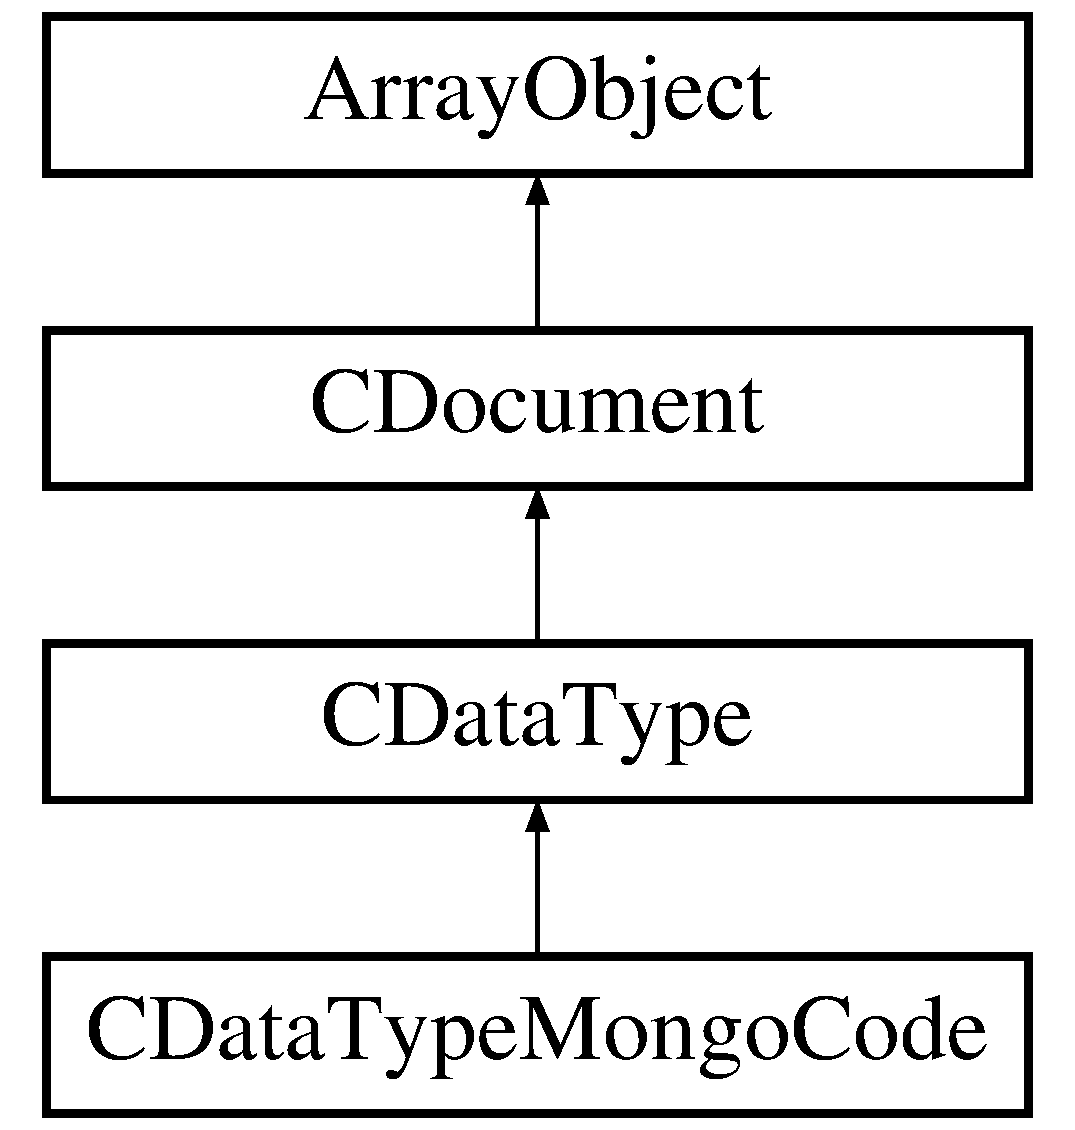
\includegraphics[height=4.000000cm]{class_c_data_type_mongo_code}
\end{center}
\end{figure}
\subsection*{Public Member Functions}
\begin{DoxyCompactItemize}
\item 
\hyperlink{class_c_data_type_mongo_code_a7eb2c6590e0a7ba7e5080a0953779786}{\-\_\-\-\_\-construct} (\$the\-Data=N\-U\-L\-L)
\item 
\hyperlink{class_c_data_type_mongo_code_a2f0db89da0c74ad4cfb3b0826aaefb70}{value} ()
\end{DoxyCompactItemize}
\subsection*{Additional Inherited Members}


\subsection{Constructor \& Destructor Documentation}
\hypertarget{class_c_data_type_mongo_code_a7eb2c6590e0a7ba7e5080a0953779786}{\index{C\-Data\-Type\-Mongo\-Code@{C\-Data\-Type\-Mongo\-Code}!\-\_\-\-\_\-construct@{\-\_\-\-\_\-construct}}
\index{\-\_\-\-\_\-construct@{\-\_\-\-\_\-construct}!CDataTypeMongoCode@{C\-Data\-Type\-Mongo\-Code}}
\subsubsection[{\-\_\-\-\_\-construct}]{\setlength{\rightskip}{0pt plus 5cm}C\-Data\-Type\-Mongo\-Code\-::\-\_\-\-\_\-construct (
\begin{DoxyParamCaption}
\item[{}]{\$the\-Data = {\ttfamily NULL}}
\end{DoxyParamCaption}
)}}\label{class_c_data_type_mongo_code_a7eb2c6590e0a7ba7e5080a0953779786}
Instantiate class.

In this class we can only instantiate such an object from a Mongo\-Code object.


\begin{DoxyParams}[1]{Parameters}
mixed & {\em \$the\-Data} & Custom data.\\
\hline
\end{DoxyParams}
public


\begin{DoxyExceptions}{Exceptions}
{\em Exception} & \\
\hline
\end{DoxyExceptions}


\subsection{Member Function Documentation}
\hypertarget{class_c_data_type_mongo_code_a2f0db89da0c74ad4cfb3b0826aaefb70}{\index{C\-Data\-Type\-Mongo\-Code@{C\-Data\-Type\-Mongo\-Code}!value@{value}}
\index{value@{value}!CDataTypeMongoCode@{C\-Data\-Type\-Mongo\-Code}}
\subsubsection[{value}]{\setlength{\rightskip}{0pt plus 5cm}C\-Data\-Type\-Mongo\-Code\-::value (
\begin{DoxyParamCaption}
{}
\end{DoxyParamCaption}
)}}\label{class_c_data_type_mongo_code_a2f0db89da0c74ad4cfb3b0826aaefb70}
Return data value.

In this class we return the Mongo\-Code object.

public \begin{DoxyReturn}{Returns}
mixed
\end{DoxyReturn}

\begin{DoxyExceptions}{Exceptions}
{\em Exception} & \\
\hline
\end{DoxyExceptions}


The documentation for this class was generated from the following file\-:\begin{DoxyCompactItemize}
\item 
/\-Library/\-Web\-Server/\-Library/\-P\-H\-P\-Wrapper/classes/C\-Data\-Type\-Mongo\-Code.\-php\end{DoxyCompactItemize}

\hypertarget{class_c_data_type_mongo_id}{\section{C\-Data\-Type\-Mongo\-Id Class Reference}
\label{class_c_data_type_mongo_id}\index{C\-Data\-Type\-Mongo\-Id@{C\-Data\-Type\-Mongo\-Id}}
}
Inheritance diagram for C\-Data\-Type\-Mongo\-Id\-:\begin{figure}[H]
\begin{center}
\leavevmode
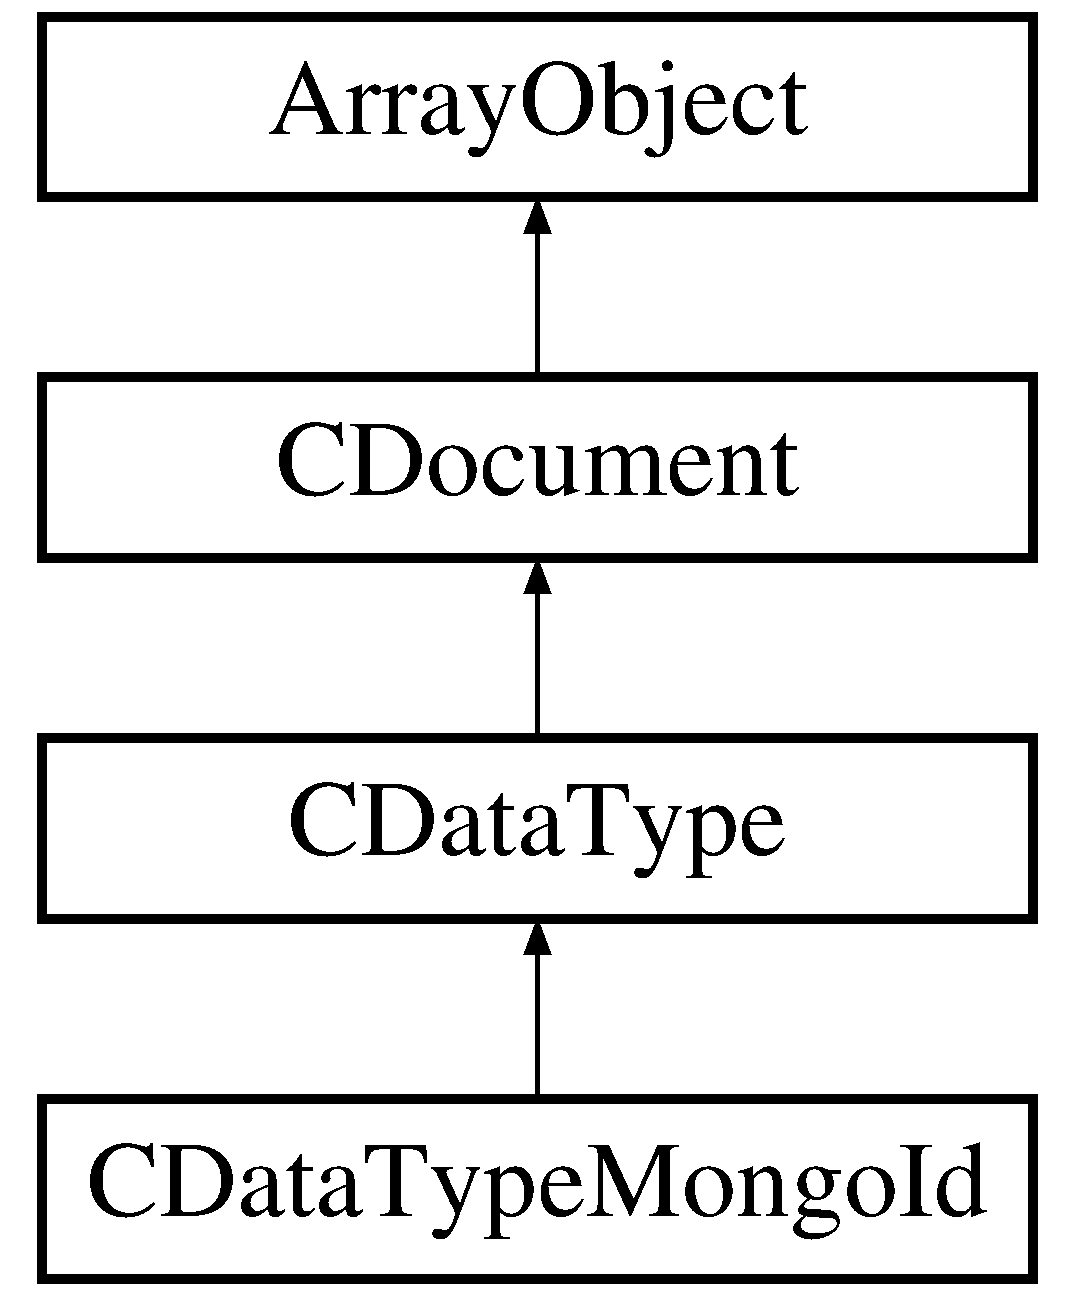
\includegraphics[height=4.000000cm]{class_c_data_type_mongo_id}
\end{center}
\end{figure}
\subsection*{Public Member Functions}
\begin{DoxyCompactItemize}
\item 
\hyperlink{class_c_data_type_mongo_id_a74cbfbb617dfdba49779b4392d01ccb2}{\-\_\-\-\_\-construct} (\$the\-Data=N\-U\-L\-L)
\item 
\hyperlink{class_c_data_type_mongo_id_a24bd5d314b38fcb049d6600de0f191df}{value} ()
\end{DoxyCompactItemize}
\subsection*{Additional Inherited Members}


\subsection{Constructor \& Destructor Documentation}
\hypertarget{class_c_data_type_mongo_id_a74cbfbb617dfdba49779b4392d01ccb2}{\index{C\-Data\-Type\-Mongo\-Id@{C\-Data\-Type\-Mongo\-Id}!\-\_\-\-\_\-construct@{\-\_\-\-\_\-construct}}
\index{\-\_\-\-\_\-construct@{\-\_\-\-\_\-construct}!CDataTypeMongoId@{C\-Data\-Type\-Mongo\-Id}}
\subsubsection[{\-\_\-\-\_\-construct}]{\setlength{\rightskip}{0pt plus 5cm}C\-Data\-Type\-Mongo\-Id\-::\-\_\-\-\_\-construct (
\begin{DoxyParamCaption}
\item[{}]{\$the\-Data = {\ttfamily NULL}}
\end{DoxyParamCaption}
)}}\label{class_c_data_type_mongo_id_a74cbfbb617dfdba49779b4392d01ccb2}
Instantiate class.

We overload the parent constructor to set the default \hyperlink{}{k\-T\-Y\-P\-E\-\_\-\-Mongo\-Id} and to set the H\-E\-X string into the \hyperlink{}{k\-T\-A\-G\-\_\-\-C\-U\-S\-T\-O\-M\-\_\-\-D\-A\-T\-A} offset.


\begin{DoxyParams}[1]{Parameters}
mixed & {\em \$the\-Data} & Custom data.\\
\hline
\end{DoxyParams}
public


\begin{DoxyExceptions}{Exceptions}
{\em Exception} & \\
\hline
\end{DoxyExceptions}


\subsection{Member Function Documentation}
\hypertarget{class_c_data_type_mongo_id_a24bd5d314b38fcb049d6600de0f191df}{\index{C\-Data\-Type\-Mongo\-Id@{C\-Data\-Type\-Mongo\-Id}!value@{value}}
\index{value@{value}!CDataTypeMongoId@{C\-Data\-Type\-Mongo\-Id}}
\subsubsection[{value}]{\setlength{\rightskip}{0pt plus 5cm}C\-Data\-Type\-Mongo\-Id\-::value (
\begin{DoxyParamCaption}
{}
\end{DoxyParamCaption}
)}}\label{class_c_data_type_mongo_id_a24bd5d314b38fcb049d6600de0f191df}
Return data value.

In this class we return the Mongo\-Id object.

public \begin{DoxyReturn}{Returns}
mixed
\end{DoxyReturn}

\begin{DoxyExceptions}{Exceptions}
{\em Exception} & \\
\hline
\end{DoxyExceptions}


The documentation for this class was generated from the following file\-:\begin{DoxyCompactItemize}
\item 
/\-Library/\-Web\-Server/\-Library/\-P\-H\-P\-Wrapper/classes/C\-Data\-Type\-Mongo\-Id.\-php\end{DoxyCompactItemize}

\hypertarget{class_c_data_type_regex}{\section{C\-Data\-Type\-Regex Class Reference}
\label{class_c_data_type_regex}\index{C\-Data\-Type\-Regex@{C\-Data\-Type\-Regex}}
}
Inheritance diagram for C\-Data\-Type\-Regex\-:\begin{figure}[H]
\begin{center}
\leavevmode
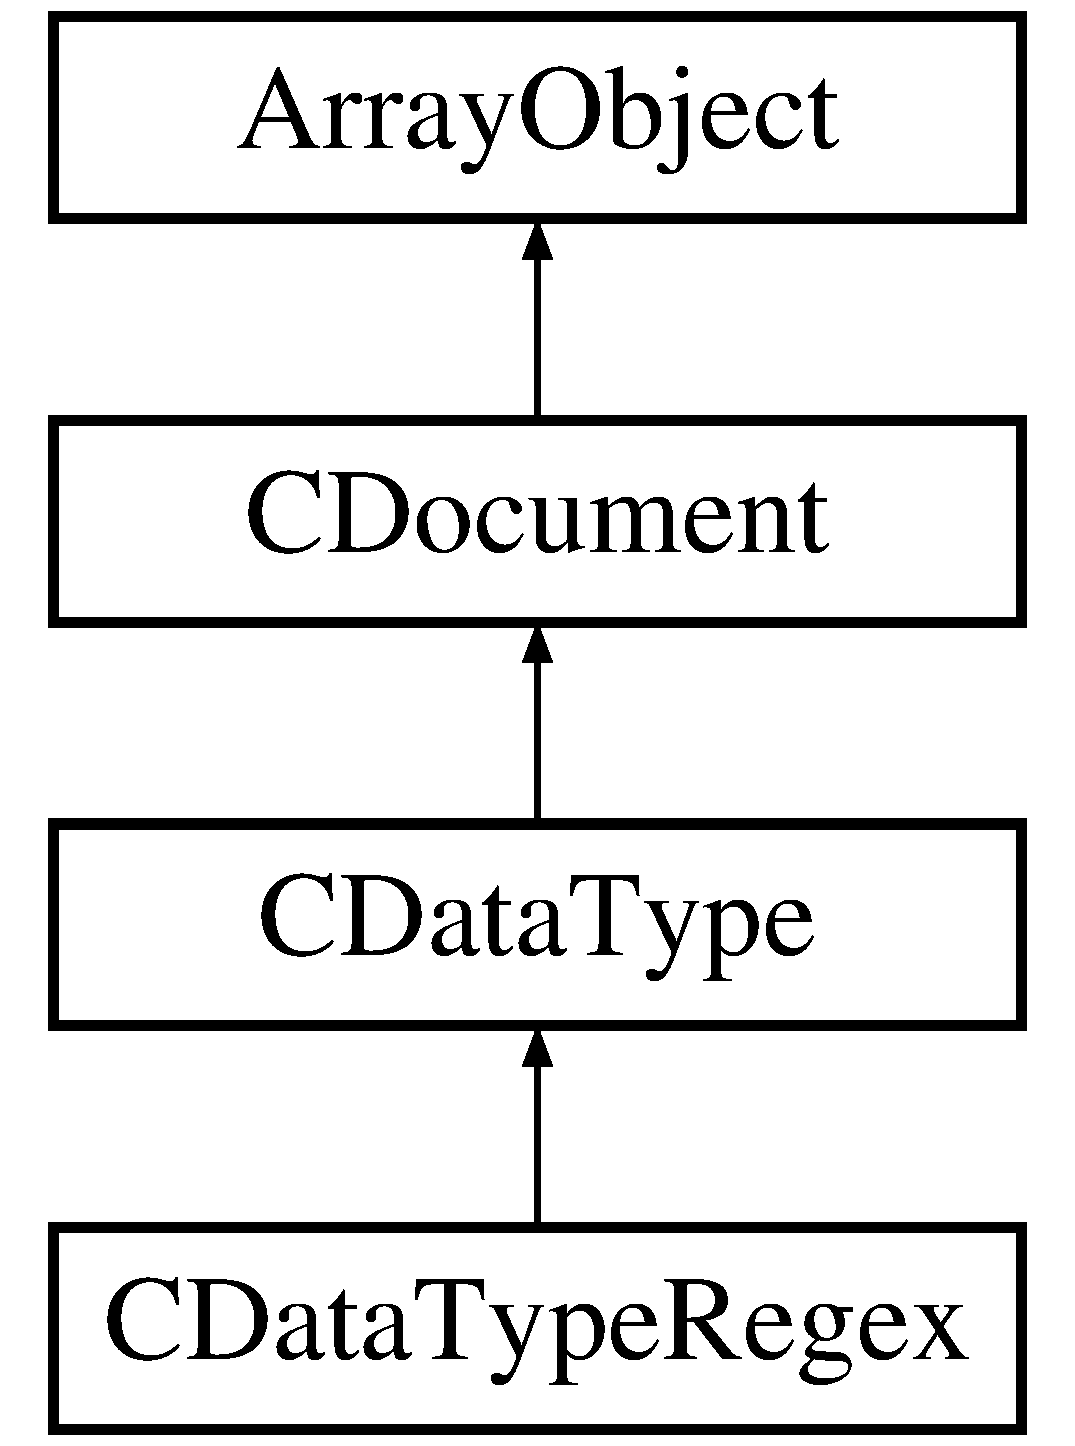
\includegraphics[height=4.000000cm]{class_c_data_type_regex}
\end{center}
\end{figure}
\subsection*{Public Member Functions}
\begin{DoxyCompactItemize}
\item 
\hyperlink{class_c_data_type_regex_a128da2b94c0b1a72fa44e656923e96d0}{\-\_\-\-\_\-construct} (\$the\-Data=N\-U\-L\-L)
\item 
\hyperlink{class_c_data_type_regex_a957186494f3c0e621540b972f51f5ea0}{value} ()
\end{DoxyCompactItemize}
\subsection*{Additional Inherited Members}


\subsection{Constructor \& Destructor Documentation}
\hypertarget{class_c_data_type_regex_a128da2b94c0b1a72fa44e656923e96d0}{\index{C\-Data\-Type\-Regex@{C\-Data\-Type\-Regex}!\-\_\-\-\_\-construct@{\-\_\-\-\_\-construct}}
\index{\-\_\-\-\_\-construct@{\-\_\-\-\_\-construct}!CDataTypeRegex@{C\-Data\-Type\-Regex}}
\subsubsection[{\-\_\-\-\_\-construct}]{\setlength{\rightskip}{0pt plus 5cm}C\-Data\-Type\-Regex\-::\-\_\-\-\_\-construct (
\begin{DoxyParamCaption}
\item[{}]{\$the\-Data = {\ttfamily NULL}}
\end{DoxyParamCaption}
)}}\label{class_c_data_type_regex_a128da2b94c0b1a72fa44e656923e96d0}
Instantiate class.

In this class we instantiate such an object from a Mongo\-Regex object or from a string.


\begin{DoxyParams}[1]{Parameters}
mixed & {\em \$the\-Data} & Custom data.\\
\hline
\end{DoxyParams}
public


\begin{DoxyExceptions}{Exceptions}
{\em Exception} & \\
\hline
\end{DoxyExceptions}


\subsection{Member Function Documentation}
\hypertarget{class_c_data_type_regex_a957186494f3c0e621540b972f51f5ea0}{\index{C\-Data\-Type\-Regex@{C\-Data\-Type\-Regex}!value@{value}}
\index{value@{value}!CDataTypeRegex@{C\-Data\-Type\-Regex}}
\subsubsection[{value}]{\setlength{\rightskip}{0pt plus 5cm}C\-Data\-Type\-Regex\-::value (
\begin{DoxyParamCaption}
{}
\end{DoxyParamCaption}
)}}\label{class_c_data_type_regex_a957186494f3c0e621540b972f51f5ea0}
Return data value.

In this class we return the Mongo\-Regex object.

public \begin{DoxyReturn}{Returns}
mixed
\end{DoxyReturn}

\begin{DoxyExceptions}{Exceptions}
{\em Exception} & \\
\hline
\end{DoxyExceptions}


The documentation for this class was generated from the following file\-:\begin{DoxyCompactItemize}
\item 
/\-Library/\-Web\-Server/\-Library/\-P\-H\-P\-Wrapper/classes/C\-Data\-Type\-Regex.\-php\end{DoxyCompactItemize}

\hypertarget{class_c_data_type_stamp}{\section{C\-Data\-Type\-Stamp Class Reference}
\label{class_c_data_type_stamp}\index{C\-Data\-Type\-Stamp@{C\-Data\-Type\-Stamp}}
}
Inheritance diagram for C\-Data\-Type\-Stamp\-:\begin{figure}[H]
\begin{center}
\leavevmode
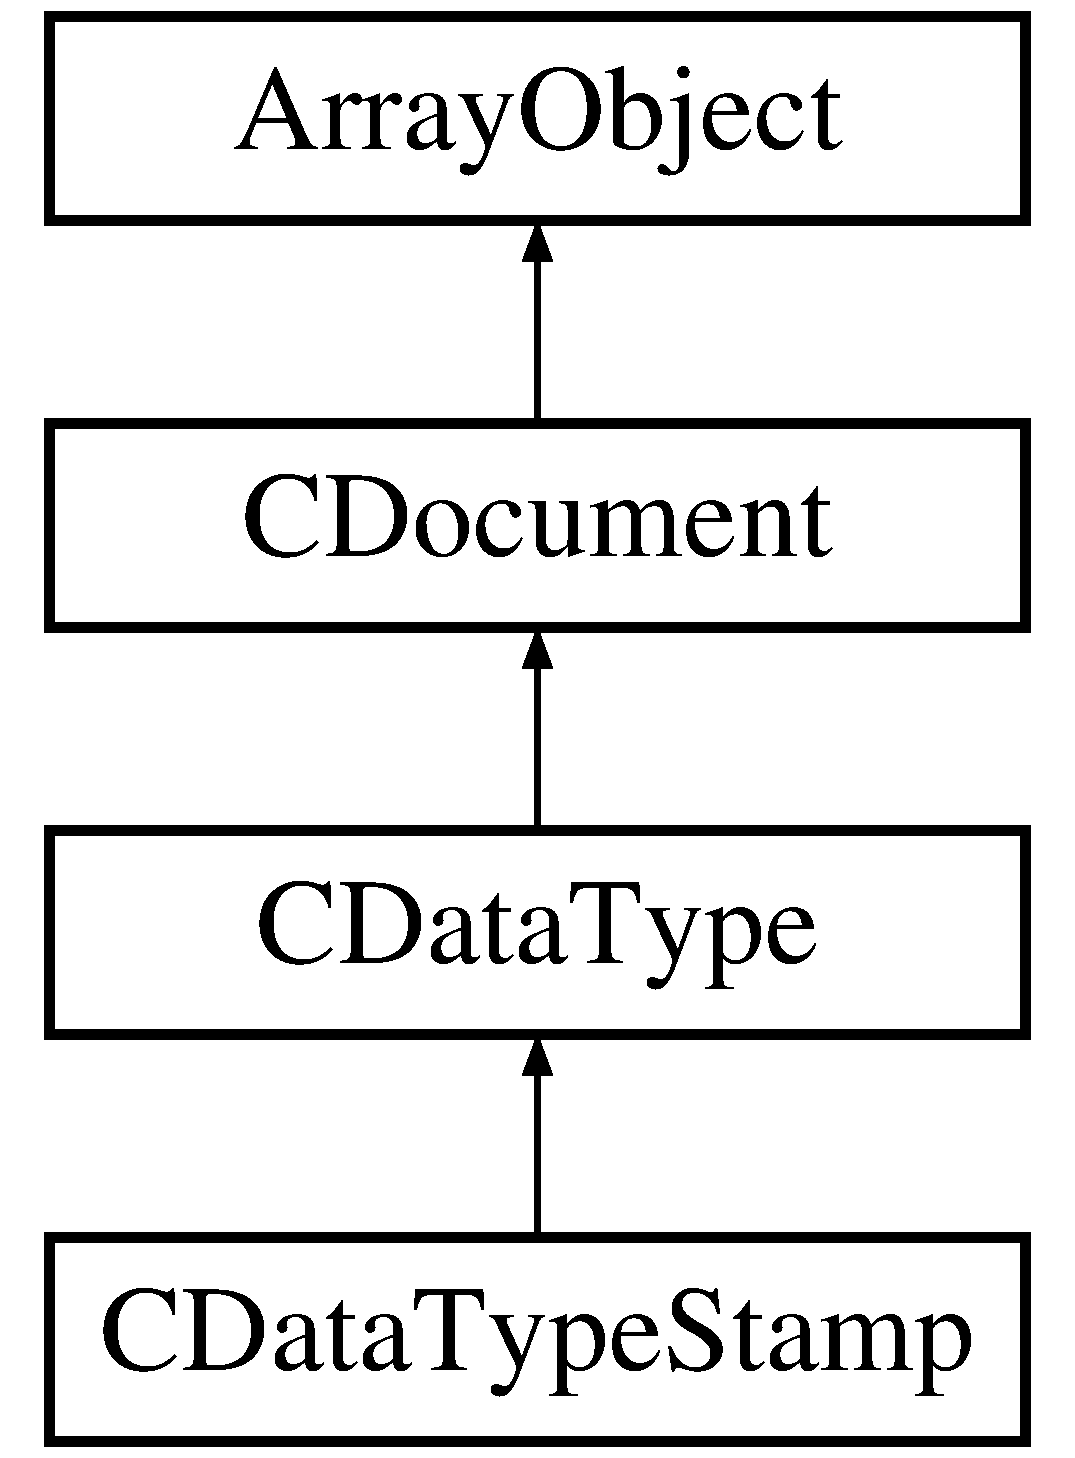
\includegraphics[height=4.000000cm]{class_c_data_type_stamp}
\end{center}
\end{figure}
\subsection*{Public Member Functions}
\begin{DoxyCompactItemize}
\item 
\hyperlink{class_c_data_type_stamp_a4ae6aac8e317e97afcf82bcd61450f52}{\-\_\-\-\_\-construct} (\$the\-Data=N\-U\-L\-L)
\item 
\hyperlink{class_c_data_type_stamp_ab0256098cc25df9b50cc765a093d2cef}{\-\_\-\-\_\-to\-String} ()
\item 
\hyperlink{class_c_data_type_stamp_ac44e6be53a7dd369c159c19a5d31056c}{value} ()
\end{DoxyCompactItemize}
\subsection*{Additional Inherited Members}


\subsection{Constructor \& Destructor Documentation}
\hypertarget{class_c_data_type_stamp_a4ae6aac8e317e97afcf82bcd61450f52}{\index{C\-Data\-Type\-Stamp@{C\-Data\-Type\-Stamp}!\-\_\-\-\_\-construct@{\-\_\-\-\_\-construct}}
\index{\-\_\-\-\_\-construct@{\-\_\-\-\_\-construct}!CDataTypeStamp@{C\-Data\-Type\-Stamp}}
\subsubsection[{\-\_\-\-\_\-construct}]{\setlength{\rightskip}{0pt plus 5cm}C\-Data\-Type\-Stamp\-::\-\_\-\-\_\-construct (
\begin{DoxyParamCaption}
\item[{}]{\$the\-Data = {\ttfamily NULL}}
\end{DoxyParamCaption}
)}}\label{class_c_data_type_stamp_a4ae6aac8e317e97afcf82bcd61450f52}
Instantiate class.

We overload the parent constructor to handle different types of data\-:


\begin{DoxyItemize}
\item {\itshape float}\-: If the data is a float, we assume it is the result of {\itshape microtime( T\-R\-U\-E )} in which the integral part of the number represents the number of seconds since January 1st 1970 G\-M\-T, and the fractional part represents the microseconds. 
\item {\itshape integer}\-: If the data is an integer, we assume it represents the number of seconds since January 1st 1970 G\-M\-T. 
\item {\itshape Mongo\-Date}\-: We use the object's elements. 
\item {\itshape Date\-Time}\-: We get the date seconds count. 
\item {\itshape other}\-: We assume the data is a date time string. 
\end{DoxyItemize}

No {\itshape N\-U\-L\-L} concrete instance is allowed, all instances derived from this class must have a value.


\begin{DoxyParams}[1]{Parameters}
mixed & {\em \$the\-Data} & Custom data.\\
\hline
\end{DoxyParams}
public


\begin{DoxyExceptions}{Exceptions}
{\em Exception} & \\
\hline
\end{DoxyExceptions}


\subsection{Member Function Documentation}
\hypertarget{class_c_data_type_stamp_ab0256098cc25df9b50cc765a093d2cef}{\index{C\-Data\-Type\-Stamp@{C\-Data\-Type\-Stamp}!\-\_\-\-\_\-to\-String@{\-\_\-\-\_\-to\-String}}
\index{\-\_\-\-\_\-to\-String@{\-\_\-\-\_\-to\-String}!CDataTypeStamp@{C\-Data\-Type\-Stamp}}
\subsubsection[{\-\_\-\-\_\-to\-String}]{\setlength{\rightskip}{0pt plus 5cm}C\-Data\-Type\-Stamp\-::\-\_\-\-\_\-to\-String (
\begin{DoxyParamCaption}
{}
\end{DoxyParamCaption}
)}}\label{class_c_data_type_stamp_ab0256098cc25df9b50cc765a093d2cef}
Return string representation.

This method should return a string representation of the custom data type contents, this method must be implemented for all concrete classes.

By default this method expects the custom data part to be convertable to string, if this is not the case, overload this method.

public \begin{DoxyReturn}{Returns}
string 
\end{DoxyReturn}
\hypertarget{class_c_data_type_stamp_ac44e6be53a7dd369c159c19a5d31056c}{\index{C\-Data\-Type\-Stamp@{C\-Data\-Type\-Stamp}!value@{value}}
\index{value@{value}!CDataTypeStamp@{C\-Data\-Type\-Stamp}}
\subsubsection[{value}]{\setlength{\rightskip}{0pt plus 5cm}C\-Data\-Type\-Stamp\-::value (
\begin{DoxyParamCaption}
{}
\end{DoxyParamCaption}
)}}\label{class_c_data_type_stamp_ac44e6be53a7dd369c159c19a5d31056c}
Return data value.

This method will return a floating point number equivalent to the result of the {\itshape microtime( T\-R\-U\-E )} function.


\begin{DoxyParams}[1]{Parameters}
reference & {\em \$the\-Struct} & Query structure.\\
\hline
\end{DoxyParams}
public \begin{DoxyReturn}{Returns}
float
\end{DoxyReturn}

\begin{DoxyExceptions}{Exceptions}
{\em Exception} & \\
\hline
\end{DoxyExceptions}


The documentation for this class was generated from the following file\-:\begin{DoxyCompactItemize}
\item 
/\-Library/\-Web\-Server/\-Library/\-P\-H\-P\-Wrapper/classes/C\-Data\-Type\-Stamp.\-php\end{DoxyCompactItemize}

\hypertarget{class_c_data_wrapper}{\section{C\-Data\-Wrapper Class Reference}
\label{class_c_data_wrapper}\index{C\-Data\-Wrapper@{C\-Data\-Wrapper}}
}
Inheritance diagram for C\-Data\-Wrapper\-:\begin{figure}[H]
\begin{center}
\leavevmode
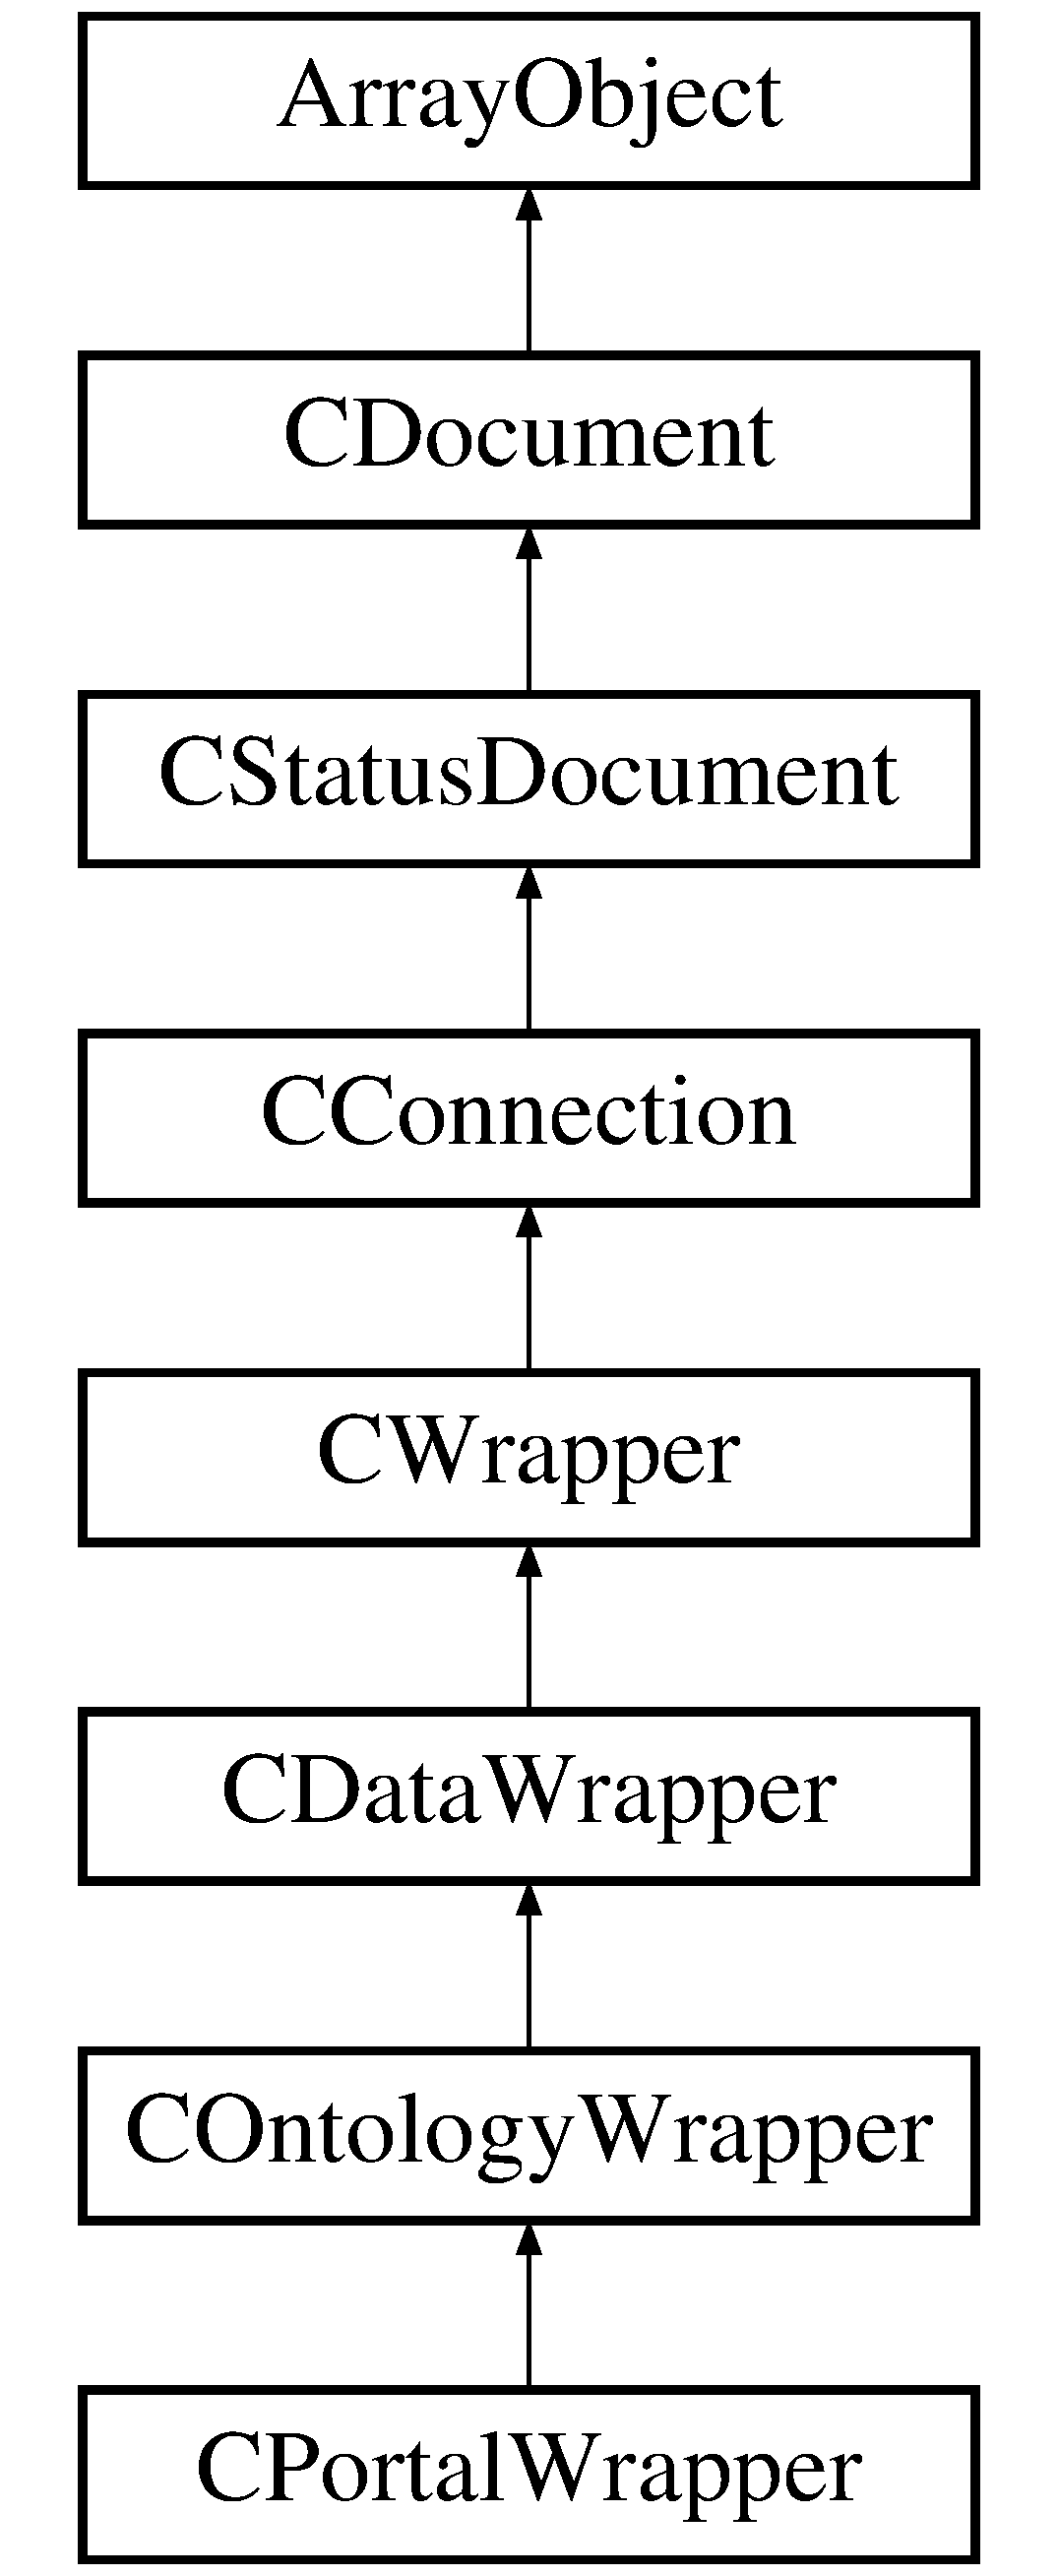
\includegraphics[height=8.000000cm]{class_c_data_wrapper}
\end{center}
\end{figure}
\subsection*{Static Public Attributes}
\begin{DoxyCompactItemize}
\item 
static {\bfseries \$s\-Parameter\-List}
\end{DoxyCompactItemize}
\subsection*{Protected Member Functions}
\begin{DoxyCompactItemize}
\item 
\hyperlink{class_c_data_wrapper_a8b42bd195d9ec6b38ef8e0df3f5dba7a}{\-\_\-\-Parse\-Request} ()
\item 
\hyperlink{class_c_data_wrapper_ab46c0e9797e8636ca1c9d535b377b90a}{\-\_\-\-Format\-Request} ()
\item 
\hyperlink{class_c_data_wrapper_aed059c9ffcb6e988633ba5b28a875b76}{\-\_\-\-Validate\-Request} ()
\item 
\hyperlink{class_c_data_wrapper_ad6d3a6b104fc3aa831cabb3271e096da}{\-\_\-\-Init\-Parameters} ()
\item 
\hyperlink{class_c_data_wrapper_a5f5f4beb1e2362c9166cf9aeb687ebc2}{\-\_\-\-Parse\-Operation} ()
\item 
\hyperlink{class_c_data_wrapper_a5bbe50542668dc7fddb133ad4ae5a839}{\-\_\-\-Parse\-Class} ()
\item 
\hyperlink{class_c_data_wrapper_afdf0880393aff6f06b29a03245bed4a5}{\-\_\-\-Parse\-Database} ()
\item 
\hyperlink{class_c_data_wrapper_a7f0f78bd3a8528562275fb6cbb2f161d}{\-\_\-\-Parse\-Container} ()
\item 
\hyperlink{class_c_data_wrapper_a3a0153df5d8c9e29e53d5060b78de785}{\-\_\-\-Parse\-Paging} ()
\item 
\hyperlink{class_c_data_wrapper_a3b0852a34c7e36ae691fa6afdfe78856}{\-\_\-\-Parse\-Query} ()
\item 
\hyperlink{class_c_data_wrapper_abf0dba3c1610c5292dd475e53e757891}{\-\_\-\-Parse\-Select} ()
\item 
\hyperlink{class_c_data_wrapper_a73cd0698e6eb033bf5500be06d3c9814}{\-\_\-\-Parse\-Sort} ()
\item 
\hyperlink{class_c_data_wrapper_a8090c59cd0c69102a8ff20a1098da31d}{\-\_\-\-Parse\-Distinct} ()
\item 
\hyperlink{class_c_data_wrapper_ab8f321158c05c2db991c35fa43b7b652}{\-\_\-\-Parse\-Object} ()
\item 
\hyperlink{class_c_data_wrapper_a1d5c10df99994e42e3b80db49276f70f}{\-\_\-\-Parse\-Criteria} ()
\item 
\hyperlink{class_c_data_wrapper_a9fc9b3bd064cfaa58920fcbfa8178abc}{\-\_\-\-Format\-Class} ()
\item 
\hyperlink{class_c_data_wrapper_a2fd22a1e55d94b6d9b65f8c56496cd3b}{\-\_\-\-Format\-Database} ()
\item 
\hyperlink{class_c_data_wrapper_a2e8e2a7f0e09c990932ae3d4b8903982}{\-\_\-\-Format\-Container} ()
\item 
\hyperlink{class_c_data_wrapper_abaf133a394b91405477d1e362496f74b}{\-\_\-\-Format\-Paging} ()
\item 
\hyperlink{class_c_data_wrapper_a0c3054fcf3716d638922cd581d5c706e}{\-\_\-\-Format\-Query} ()
\item 
\hyperlink{class_c_data_wrapper_a318ea202e1ec6a1bf0154165f2aa8576}{\-\_\-\-Format\-Select} ()
\item 
\hyperlink{class_c_data_wrapper_a040ed6e140436322b736744740cc8cbd}{\-\_\-\-Format\-Sort} ()
\item 
\hyperlink{class_c_data_wrapper_a51cd50654dd1b518c1aff08cfb9c7d46}{\-\_\-\-Format\-Distinct} ()
\item 
\hyperlink{class_c_data_wrapper_addefb7bd419de62bfebedc21abbdad7e}{\-\_\-\-Format\-Object} ()
\item 
\hyperlink{class_c_data_wrapper_a081597709126bc46a8ae4ed071b98fd4}{\-\_\-\-Format\-Criteria} ()
\item 
\hyperlink{class_c_data_wrapper_ac25dbab0dc8d55b3b8f0a4027d4549c6}{\-\_\-\-Validate\-Operation} ()
\item 
\hyperlink{class_c_data_wrapper_a0d2d8f118bf073be5d8821632d423ef5}{\-\_\-\-Validate\-Class} ()
\item 
\hyperlink{class_c_data_wrapper_a28268d756311188bc77b980823e389c4}{\-\_\-\-Validate\-Database} ()
\item 
\hyperlink{class_c_data_wrapper_a7a6620a2b6ef1de3dfad673b4d977da1}{\-\_\-\-Validate\-Container} ()
\item 
\hyperlink{class_c_data_wrapper_a794047412591b0e4dac24c5c3c93c027}{\-\_\-\-Validate\-Paging} ()
\item 
\hyperlink{class_c_data_wrapper_a647874d1600ca237ec5d6697730f2f00}{\-\_\-\-Validate\-Query} ()
\item 
\hyperlink{class_c_data_wrapper_ad62b183dc761424941781da00b616610}{\-\_\-\-Validate\-Select} ()
\item 
\hyperlink{class_c_data_wrapper_a42d14abef174cd5eddee8e050faf3268}{\-\_\-\-Validate\-Sort} ()
\item 
\hyperlink{class_c_data_wrapper_a08197265c8169d9780b19b226327a5fd}{\-\_\-\-Validate\-Distinct} ()
\item 
\hyperlink{class_c_data_wrapper_a8e8a0302f088adf0349bd6bb7110bffb}{\-\_\-\-Validate\-Object} ()
\item 
\hyperlink{class_c_data_wrapper_ac698ae477425e609df6c707fdb60a09f}{\-\_\-\-Validate\-Criteria} ()
\item 
\hyperlink{class_c_data_wrapper_a873fe1808fb645b01424caa975ae6b4e}{\-\_\-\-Handle\-Request} ()
\item 
\hyperlink{class_c_data_wrapper_afc7251c3aad9141599372d6b94904498}{\-\_\-\-Handle\-\_\-\-List\-Op} (\&\$the\-List)
\item 
\hyperlink{class_c_data_wrapper_a96f5e3613e01b469c39711e0367f1d55}{\-\_\-\-Handle\-\_\-\-Count} ()
\item 
\hyperlink{class_c_data_wrapper_acbe6ebfc205a6627281bfc7e921d51a8}{\-\_\-\-Handle\-\_\-\-Get} ()
\item 
\hyperlink{class_c_data_wrapper_a02e30005fdb1d7fd392869bbc92b08ea}{\-\_\-\-Handle\-\_\-\-Get\-One} ()
\item 
\hyperlink{class_c_data_wrapper_a3a8e8dd504dc2ead8826f06f73cbd674}{\-\_\-\-Handle\-\_\-\-Resolve} ()
\item 
\hyperlink{class_c_data_wrapper_a8c194665e3bce2f214ad9d7cfeecb19b}{\-\_\-\-Handle\-\_\-\-Insert} ()
\item 
\hyperlink{class_c_data_wrapper_aab0ed289574b05800670783825fc4a23}{\-\_\-\-Handle\-\_\-\-Modify} ()
\item 
\hyperlink{class_c_data_wrapper_a9d5f015b9ed7f3062105b846d50e4bc8}{\-\_\-\-Handle\-\_\-\-Delete} ()
\item 
\hyperlink{class_c_data_wrapper_ae9a8755012f6ed16d64a0462ae08ec6b}{\-\_\-\-Query} (\$the\-Result=N\-U\-L\-L, \$is\-Count=F\-A\-L\-S\-E, \$do\-Count=T\-R\-U\-E, \$the\-Query=N\-U\-L\-L, \$the\-Container=N\-U\-L\-L, \$the\-Selection=N\-U\-L\-L)
\item 
\hyperlink{class_c_data_wrapper_ae7ccf4b5e3fa27bfa337c8b2c752db33}{\-\_\-\-Validate\-Queries} (\&\$the\-Query, \hyperlink{class_c_container}{C\-Container} \$the\-Container)
\item 
\hyperlink{class_c_data_wrapper_ae1c1d4975d08d10165f6f4dc8a7751da}{\-\_\-\-Verify\-Query} (\&\$the\-Query, \hyperlink{class_c_container}{C\-Container} \$the\-Container)
\end{DoxyCompactItemize}
\subsection*{Additional Inherited Members}


\subsection{Member Function Documentation}
\hypertarget{class_c_data_wrapper_a9fc9b3bd064cfaa58920fcbfa8178abc}{\index{C\-Data\-Wrapper@{C\-Data\-Wrapper}!\-\_\-\-Format\-Class@{\-\_\-\-Format\-Class}}
\index{\-\_\-\-Format\-Class@{\-\_\-\-Format\-Class}!CDataWrapper@{C\-Data\-Wrapper}}
\subsubsection[{\-\_\-\-Format\-Class}]{\setlength{\rightskip}{0pt plus 5cm}C\-Data\-Wrapper\-::\-\_\-\-Format\-Class (
\begin{DoxyParamCaption}
{}
\end{DoxyParamCaption}
)\hspace{0.3cm}{\ttfamily [protected]}}}\label{class_c_data_wrapper_a9fc9b3bd064cfaa58920fcbfa8178abc}
Format class parameter.

This method will first check if the class is available, then, if the container is missing, it will set its name with the eventual \hyperlink{class_c_persistent_document_ab2fa5e1b0e3f967b8b3727eb28300652}{C\-Persistent\-Document\-::\-Default\-Container\-Name()} method.

protected

\begin{DoxySeeAlso}{See Also}
k\-A\-P\-I\-\_\-\-C\-L\-A\-S\-S 
\end{DoxySeeAlso}
\hypertarget{class_c_data_wrapper_a2e8e2a7f0e09c990932ae3d4b8903982}{\index{C\-Data\-Wrapper@{C\-Data\-Wrapper}!\-\_\-\-Format\-Container@{\-\_\-\-Format\-Container}}
\index{\-\_\-\-Format\-Container@{\-\_\-\-Format\-Container}!CDataWrapper@{C\-Data\-Wrapper}}
\subsubsection[{\-\_\-\-Format\-Container}]{\setlength{\rightskip}{0pt plus 5cm}C\-Data\-Wrapper\-::\-\_\-\-Format\-Container (
\begin{DoxyParamCaption}
{}
\end{DoxyParamCaption}
)\hspace{0.3cm}{\ttfamily [protected]}}}\label{class_c_data_wrapper_a2e8e2a7f0e09c990932ae3d4b8903982}
Instantiate container.

This method will instantiate the \hyperlink{class_c_container}{C\-Container} instance if the name was provided as parameter. If the \hyperlink{}{k\-A\-P\-I\-\_\-\-D\-A\-T\-A\-B\-A\-S\-E} element is not set, the method will raise an exception.

protected

\begin{DoxySeeAlso}{See Also}
k\-A\-P\-I\-\_\-\-C\-O\-N\-T\-A\-I\-N\-E\-R 
\end{DoxySeeAlso}
\hypertarget{class_c_data_wrapper_a081597709126bc46a8ae4ed071b98fd4}{\index{C\-Data\-Wrapper@{C\-Data\-Wrapper}!\-\_\-\-Format\-Criteria@{\-\_\-\-Format\-Criteria}}
\index{\-\_\-\-Format\-Criteria@{\-\_\-\-Format\-Criteria}!CDataWrapper@{C\-Data\-Wrapper}}
\subsubsection[{\-\_\-\-Format\-Criteria}]{\setlength{\rightskip}{0pt plus 5cm}C\-Data\-Wrapper\-::\-\_\-\-Format\-Criteria (
\begin{DoxyParamCaption}
{}
\end{DoxyParamCaption}
)\hspace{0.3cm}{\ttfamily [protected]}}}\label{class_c_data_wrapper_a081597709126bc46a8ae4ed071b98fd4}
Format modification criteria parameter.

This method does nothing in this class.

protected

\begin{DoxySeeAlso}{See Also}
k\-A\-P\-I\-\_\-\-C\-R\-I\-T\-E\-R\-I\-A 
\end{DoxySeeAlso}
\hypertarget{class_c_data_wrapper_a2fd22a1e55d94b6d9b65f8c56496cd3b}{\index{C\-Data\-Wrapper@{C\-Data\-Wrapper}!\-\_\-\-Format\-Database@{\-\_\-\-Format\-Database}}
\index{\-\_\-\-Format\-Database@{\-\_\-\-Format\-Database}!CDataWrapper@{C\-Data\-Wrapper}}
\subsubsection[{\-\_\-\-Format\-Database}]{\setlength{\rightskip}{0pt plus 5cm}C\-Data\-Wrapper\-::\-\_\-\-Format\-Database (
\begin{DoxyParamCaption}
{}
\end{DoxyParamCaption}
)\hspace{0.3cm}{\ttfamily [protected]}}}\label{class_c_data_wrapper_a2fd22a1e55d94b6d9b65f8c56496cd3b}
Instantiate database.

This method will instantiate the \hyperlink{class_c_database}{C\-Database} instance if the name was provided as parameter. If the \hyperlink{}{k\-A\-P\-I\-\_\-\-S\-E\-R\-V\-E\-R} element is not set, the method will raise an exception.

protected

\begin{DoxySeeAlso}{See Also}
k\-A\-P\-I\-\_\-\-D\-A\-T\-A\-B\-A\-S\-E 
\end{DoxySeeAlso}
\hypertarget{class_c_data_wrapper_a51cd50654dd1b518c1aff08cfb9c7d46}{\index{C\-Data\-Wrapper@{C\-Data\-Wrapper}!\-\_\-\-Format\-Distinct@{\-\_\-\-Format\-Distinct}}
\index{\-\_\-\-Format\-Distinct@{\-\_\-\-Format\-Distinct}!CDataWrapper@{C\-Data\-Wrapper}}
\subsubsection[{\-\_\-\-Format\-Distinct}]{\setlength{\rightskip}{0pt plus 5cm}C\-Data\-Wrapper\-::\-\_\-\-Format\-Distinct (
\begin{DoxyParamCaption}
{}
\end{DoxyParamCaption}
)\hspace{0.3cm}{\ttfamily [protected]}}}\label{class_c_data_wrapper_a51cd50654dd1b518c1aff08cfb9c7d46}
Format distinct values property parameter.

In this class we do not format it.

protected

\begin{DoxySeeAlso}{See Also}
k\-A\-P\-I\-\_\-\-D\-I\-S\-T\-I\-N\-C\-T 
\end{DoxySeeAlso}
\hypertarget{class_c_data_wrapper_addefb7bd419de62bfebedc21abbdad7e}{\index{C\-Data\-Wrapper@{C\-Data\-Wrapper}!\-\_\-\-Format\-Object@{\-\_\-\-Format\-Object}}
\index{\-\_\-\-Format\-Object@{\-\_\-\-Format\-Object}!CDataWrapper@{C\-Data\-Wrapper}}
\subsubsection[{\-\_\-\-Format\-Object}]{\setlength{\rightskip}{0pt plus 5cm}C\-Data\-Wrapper\-::\-\_\-\-Format\-Object (
\begin{DoxyParamCaption}
{}
\end{DoxyParamCaption}
)\hspace{0.3cm}{\ttfamily [protected]}}}\label{class_c_data_wrapper_addefb7bd419de62bfebedc21abbdad7e}
Format object parameter.

This method does nothing in this class.

protected

\begin{DoxySeeAlso}{See Also}
k\-A\-P\-I\-\_\-\-O\-B\-J\-E\-C\-T 
\end{DoxySeeAlso}
\hypertarget{class_c_data_wrapper_abaf133a394b91405477d1e362496f74b}{\index{C\-Data\-Wrapper@{C\-Data\-Wrapper}!\-\_\-\-Format\-Paging@{\-\_\-\-Format\-Paging}}
\index{\-\_\-\-Format\-Paging@{\-\_\-\-Format\-Paging}!CDataWrapper@{C\-Data\-Wrapper}}
\subsubsection[{\-\_\-\-Format\-Paging}]{\setlength{\rightskip}{0pt plus 5cm}C\-Data\-Wrapper\-::\-\_\-\-Format\-Paging (
\begin{DoxyParamCaption}
{}
\end{DoxyParamCaption}
)\hspace{0.3cm}{\ttfamily [protected]}}}\label{class_c_data_wrapper_abaf133a394b91405477d1e362496f74b}
Format paging parameters.

This method will complete eventual missing paging parameters and fill the response \hyperlink{}{k\-A\-P\-I\-\_\-\-P\-A\-G\-I\-N\-G} block with the provided paging options.

protected

\begin{DoxySeeAlso}{See Also}
k\-A\-P\-I\-\_\-\-P\-A\-G\-I\-N\-G k\-A\-P\-I\-\_\-\-P\-A\-G\-E\-\_\-\-S\-T\-A\-R\-T k\-A\-P\-I\-\_\-\-P\-A\-G\-E\-\_\-\-L\-I\-M\-I\-T 
\end{DoxySeeAlso}
\hypertarget{class_c_data_wrapper_a0c3054fcf3716d638922cd581d5c706e}{\index{C\-Data\-Wrapper@{C\-Data\-Wrapper}!\-\_\-\-Format\-Query@{\-\_\-\-Format\-Query}}
\index{\-\_\-\-Format\-Query@{\-\_\-\-Format\-Query}!CDataWrapper@{C\-Data\-Wrapper}}
\subsubsection[{\-\_\-\-Format\-Query}]{\setlength{\rightskip}{0pt plus 5cm}C\-Data\-Wrapper\-::\-\_\-\-Format\-Query (
\begin{DoxyParamCaption}
{}
\end{DoxyParamCaption}
)\hspace{0.3cm}{\ttfamily [protected]}}}\label{class_c_data_wrapper_a0c3054fcf3716d638922cd581d5c706e}
Format query.

The main duty of this method is to format the provided query. This parameter will be provided as an array in which the first level element indexes can take the following values\-:


\begin{DoxyItemize}
\item {\itshape Conditional Operator}\-: If any of \hyperlink{}{k\-O\-P\-E\-R\-A\-T\-O\-R\-\_\-\-A\-N\-D}, \hyperlink{}{k\-O\-P\-E\-R\-A\-T\-O\-R\-\_\-\-O\-R}, \hyperlink{}{k\-O\-P\-E\-R\-A\-T\-O\-R\-\_\-\-N\-A\-N\-D} or \hyperlink{}{k\-O\-P\-E\-R\-A\-T\-O\-R\-\_\-\-N\-O\-R} is found as index, it means that the query is applied to the provided container. 
\item {\ttfamily integer}\-: An integer index indicates that the provided query is a list of queries for the container provided to the service. 
\item {\itshape other}\-: Any other kind of data will be cast to a string and interpreted as the container name. 
\end{DoxyItemize}

In this class we do nothing, derived classes may overload this method to customise the structure before it gets validated.

protected

\begin{DoxySeeAlso}{See Also}
k\-A\-P\-I\-\_\-\-Q\-U\-E\-R\-Y 
\end{DoxySeeAlso}
\hypertarget{class_c_data_wrapper_ab46c0e9797e8636ca1c9d535b377b90a}{\index{C\-Data\-Wrapper@{C\-Data\-Wrapper}!\-\_\-\-Format\-Request@{\-\_\-\-Format\-Request}}
\index{\-\_\-\-Format\-Request@{\-\_\-\-Format\-Request}!CDataWrapper@{C\-Data\-Wrapper}}
\subsubsection[{\-\_\-\-Format\-Request}]{\setlength{\rightskip}{0pt plus 5cm}C\-Data\-Wrapper\-::\-\_\-\-Format\-Request (
\begin{DoxyParamCaption}
{}
\end{DoxyParamCaption}
)\hspace{0.3cm}{\ttfamily [protected]}}}\label{class_c_data_wrapper_ab46c0e9797e8636ca1c9d535b377b90a}
Format request.

This method should perform any needed formatting before the request will be handled.

In this class we handle the parameters to be decoded

protected

\hyperlink{class_c_data_wrapper_a9fc9b3bd064cfaa58920fcbfa8178abc}{\-\_\-\-Format\-Class()}  \hyperlink{class_c_data_wrapper_a2fd22a1e55d94b6d9b65f8c56496cd3b}{\-\_\-\-Format\-Database()}  \hyperlink{class_c_data_wrapper_a2e8e2a7f0e09c990932ae3d4b8903982}{\-\_\-\-Format\-Container()}  \hyperlink{class_c_data_wrapper_abaf133a394b91405477d1e362496f74b}{\-\_\-\-Format\-Paging()}  \hyperlink{class_c_data_wrapper_a0c3054fcf3716d638922cd581d5c706e}{\-\_\-\-Format\-Query()}  \hyperlink{class_c_data_wrapper_a318ea202e1ec6a1bf0154165f2aa8576}{\-\_\-\-Format\-Select()}  \hyperlink{class_c_data_wrapper_a040ed6e140436322b736744740cc8cbd}{\-\_\-\-Format\-Sort()}  \hyperlink{class_c_data_wrapper_a51cd50654dd1b518c1aff08cfb9c7d46}{\-\_\-\-Format\-Distinct()}  \hyperlink{class_c_data_wrapper_addefb7bd419de62bfebedc21abbdad7e}{\-\_\-\-Format\-Object()}  \hyperlink{class_c_data_wrapper_a081597709126bc46a8ae4ed071b98fd4}{\-\_\-\-Format\-Criteria()} \hypertarget{class_c_data_wrapper_a318ea202e1ec6a1bf0154165f2aa8576}{\index{C\-Data\-Wrapper@{C\-Data\-Wrapper}!\-\_\-\-Format\-Select@{\-\_\-\-Format\-Select}}
\index{\-\_\-\-Format\-Select@{\-\_\-\-Format\-Select}!CDataWrapper@{C\-Data\-Wrapper}}
\subsubsection[{\-\_\-\-Format\-Select}]{\setlength{\rightskip}{0pt plus 5cm}C\-Data\-Wrapper\-::\-\_\-\-Format\-Select (
\begin{DoxyParamCaption}
{}
\end{DoxyParamCaption}
)\hspace{0.3cm}{\ttfamily [protected]}}}\label{class_c_data_wrapper_a318ea202e1ec6a1bf0154165f2aa8576}
Format selection parameters.

This method will create an array from a scalar, if necessary.

protected

\begin{DoxySeeAlso}{See Also}
k\-A\-P\-I\-\_\-\-S\-E\-L\-E\-C\-T 
\end{DoxySeeAlso}
\hypertarget{class_c_data_wrapper_a040ed6e140436322b736744740cc8cbd}{\index{C\-Data\-Wrapper@{C\-Data\-Wrapper}!\-\_\-\-Format\-Sort@{\-\_\-\-Format\-Sort}}
\index{\-\_\-\-Format\-Sort@{\-\_\-\-Format\-Sort}!CDataWrapper@{C\-Data\-Wrapper}}
\subsubsection[{\-\_\-\-Format\-Sort}]{\setlength{\rightskip}{0pt plus 5cm}C\-Data\-Wrapper\-::\-\_\-\-Format\-Sort (
\begin{DoxyParamCaption}
{}
\end{DoxyParamCaption}
)\hspace{0.3cm}{\ttfamily [protected]}}}\label{class_c_data_wrapper_a040ed6e140436322b736744740cc8cbd}
Format selection parameters.

This method will create an array from a scalar, if necessary.

protected

\begin{DoxySeeAlso}{See Also}
k\-A\-P\-I\-\_\-\-S\-O\-R\-T 
\end{DoxySeeAlso}
\hypertarget{class_c_data_wrapper_a96f5e3613e01b469c39711e0367f1d55}{\index{C\-Data\-Wrapper@{C\-Data\-Wrapper}!\-\_\-\-Handle\-\_\-\-Count@{\-\_\-\-Handle\-\_\-\-Count}}
\index{\-\_\-\-Handle\-\_\-\-Count@{\-\_\-\-Handle\-\_\-\-Count}!CDataWrapper@{C\-Data\-Wrapper}}
\subsubsection[{\-\_\-\-Handle\-\_\-\-Count}]{\setlength{\rightskip}{0pt plus 5cm}C\-Data\-Wrapper\-::\-\_\-\-Handle\-\_\-\-Count (
\begin{DoxyParamCaption}
{}
\end{DoxyParamCaption}
)\hspace{0.3cm}{\ttfamily [protected]}}}\label{class_c_data_wrapper_a96f5e3613e01b469c39711e0367f1d55}
Handle \hyperlink{}{k\-A\-P\-I\-\_\-\-O\-P\-\_\-\-C\-O\-U\-N\-T} request.

This method will handle the \hyperlink{}{k\-A\-P\-I\-\_\-\-O\-P\-\_\-\-C\-O\-U\-N\-T} operation, which returns the total count of a query in the \hyperlink{}{k\-A\-P\-I\-\_\-\-A\-F\-F\-E\-C\-T\-E\-D\-\_\-\-C\-O\-U\-N\-T} field of the status.

protected \hypertarget{class_c_data_wrapper_a9d5f015b9ed7f3062105b846d50e4bc8}{\index{C\-Data\-Wrapper@{C\-Data\-Wrapper}!\-\_\-\-Handle\-\_\-\-Delete@{\-\_\-\-Handle\-\_\-\-Delete}}
\index{\-\_\-\-Handle\-\_\-\-Delete@{\-\_\-\-Handle\-\_\-\-Delete}!CDataWrapper@{C\-Data\-Wrapper}}
\subsubsection[{\-\_\-\-Handle\-\_\-\-Delete}]{\setlength{\rightskip}{0pt plus 5cm}C\-Data\-Wrapper\-::\-\_\-\-Handle\-\_\-\-Delete (
\begin{DoxyParamCaption}
{}
\end{DoxyParamCaption}
)\hspace{0.3cm}{\ttfamily [protected]}}}\label{class_c_data_wrapper_a9d5f015b9ed7f3062105b846d50e4bc8}
Handle \hyperlink{}{k\-A\-P\-I\-\_\-\-O\-P\-\_\-\-D\-E\-L\-E\-T\-E} request.

This method will handle the \hyperlink{}{k\-A\-P\-I\-\_\-\-O\-P\-\_\-\-D\-E\-L\-E\-T\-E} operation, which deletes objects matching the provided query or value.

protected \hypertarget{class_c_data_wrapper_acbe6ebfc205a6627281bfc7e921d51a8}{\index{C\-Data\-Wrapper@{C\-Data\-Wrapper}!\-\_\-\-Handle\-\_\-\-Get@{\-\_\-\-Handle\-\_\-\-Get}}
\index{\-\_\-\-Handle\-\_\-\-Get@{\-\_\-\-Handle\-\_\-\-Get}!CDataWrapper@{C\-Data\-Wrapper}}
\subsubsection[{\-\_\-\-Handle\-\_\-\-Get}]{\setlength{\rightskip}{0pt plus 5cm}C\-Data\-Wrapper\-::\-\_\-\-Handle\-\_\-\-Get (
\begin{DoxyParamCaption}
{}
\end{DoxyParamCaption}
)\hspace{0.3cm}{\ttfamily [protected]}}}\label{class_c_data_wrapper_acbe6ebfc205a6627281bfc7e921d51a8}
Handle \hyperlink{}{k\-A\-P\-I\-\_\-\-O\-P\-\_\-\-G\-E\-T} request.

This method will handle the \hyperlink{}{k\-A\-P\-I\-\_\-\-O\-P\-\_\-\-G\-E\-T} operation, which returns the records that match the provided query.

protected \hypertarget{class_c_data_wrapper_a02e30005fdb1d7fd392869bbc92b08ea}{\index{C\-Data\-Wrapper@{C\-Data\-Wrapper}!\-\_\-\-Handle\-\_\-\-Get\-One@{\-\_\-\-Handle\-\_\-\-Get\-One}}
\index{\-\_\-\-Handle\-\_\-\-Get\-One@{\-\_\-\-Handle\-\_\-\-Get\-One}!CDataWrapper@{C\-Data\-Wrapper}}
\subsubsection[{\-\_\-\-Handle\-\_\-\-Get\-One}]{\setlength{\rightskip}{0pt plus 5cm}C\-Data\-Wrapper\-::\-\_\-\-Handle\-\_\-\-Get\-One (
\begin{DoxyParamCaption}
{}
\end{DoxyParamCaption}
)\hspace{0.3cm}{\ttfamily [protected]}}}\label{class_c_data_wrapper_a02e30005fdb1d7fd392869bbc92b08ea}
Handle \hyperlink{}{k\-A\-P\-I\-\_\-\-O\-P\-\_\-\-G\-E\-T\-\_\-\-O\-N\-E} request.

This method will handle the \hyperlink{}{k\-A\-P\-I\-\_\-\-O\-P\-\_\-\-G\-E\-T\-\_\-\-O\-N\-E} operation, which returns the first record to satisfy a query.

protected \hypertarget{class_c_data_wrapper_a8c194665e3bce2f214ad9d7cfeecb19b}{\index{C\-Data\-Wrapper@{C\-Data\-Wrapper}!\-\_\-\-Handle\-\_\-\-Insert@{\-\_\-\-Handle\-\_\-\-Insert}}
\index{\-\_\-\-Handle\-\_\-\-Insert@{\-\_\-\-Handle\-\_\-\-Insert}!CDataWrapper@{C\-Data\-Wrapper}}
\subsubsection[{\-\_\-\-Handle\-\_\-\-Insert}]{\setlength{\rightskip}{0pt plus 5cm}C\-Data\-Wrapper\-::\-\_\-\-Handle\-\_\-\-Insert (
\begin{DoxyParamCaption}
{}
\end{DoxyParamCaption}
)\hspace{0.3cm}{\ttfamily [protected]}}}\label{class_c_data_wrapper_a8c194665e3bce2f214ad9d7cfeecb19b}
Handle \hyperlink{}{k\-A\-P\-I\-\_\-\-O\-P\-\_\-\-I\-N\-S\-E\-R\-T} request.

This method will handle the \hyperlink{}{k\-A\-P\-I\-\_\-\-O\-P\-\_\-\-I\-N\-S\-E\-R\-T} operation, which inserts the provided object as an instance of the provided class into the provided database or container.

This service works in two different modes\-:


\begin{DoxyItemize}
\item {\itshape \hyperlink{}{k\-A\-P\-I\-\_\-\-C\-L\-A\-S\-S} provided}\-: In this case we let the object handle the operation, which will trigger all automatic procedures for that specific class. 
\item {\itshape \hyperlink{}{k\-A\-P\-I\-\_\-\-C\-L\-A\-S\-S} not provided}\-: In this case we simply add the provided document to the provided container as-\/is. 
\end{DoxyItemize}

protected \hypertarget{class_c_data_wrapper_afc7251c3aad9141599372d6b94904498}{\index{C\-Data\-Wrapper@{C\-Data\-Wrapper}!\-\_\-\-Handle\-\_\-\-List\-Op@{\-\_\-\-Handle\-\_\-\-List\-Op}}
\index{\-\_\-\-Handle\-\_\-\-List\-Op@{\-\_\-\-Handle\-\_\-\-List\-Op}!CDataWrapper@{C\-Data\-Wrapper}}
\subsubsection[{\-\_\-\-Handle\-\_\-\-List\-Op}]{\setlength{\rightskip}{0pt plus 5cm}C\-Data\-Wrapper\-::\-\_\-\-Handle\-\_\-\-List\-Op (
\begin{DoxyParamCaption}
\item[{\&}]{\$the\-List}
\end{DoxyParamCaption}
)\hspace{0.3cm}{\ttfamily [protected]}}}\label{class_c_data_wrapper_afc7251c3aad9141599372d6b94904498}
Handle \hyperlink{}{k\-A\-P\-I\-\_\-\-O\-P\-\_\-\-H\-E\-L\-P} operations request.

This method will handle the locally supported operations.


\begin{DoxyParams}[1]{Parameters}
reference & {\em \$the\-List} & Receives operations list.\\
\hline
\end{DoxyParams}
protected \hypertarget{class_c_data_wrapper_aab0ed289574b05800670783825fc4a23}{\index{C\-Data\-Wrapper@{C\-Data\-Wrapper}!\-\_\-\-Handle\-\_\-\-Modify@{\-\_\-\-Handle\-\_\-\-Modify}}
\index{\-\_\-\-Handle\-\_\-\-Modify@{\-\_\-\-Handle\-\_\-\-Modify}!CDataWrapper@{C\-Data\-Wrapper}}
\subsubsection[{\-\_\-\-Handle\-\_\-\-Modify}]{\setlength{\rightskip}{0pt plus 5cm}C\-Data\-Wrapper\-::\-\_\-\-Handle\-\_\-\-Modify (
\begin{DoxyParamCaption}
{}
\end{DoxyParamCaption}
)\hspace{0.3cm}{\ttfamily [protected]}}}\label{class_c_data_wrapper_aab0ed289574b05800670783825fc4a23}
Handle \hyperlink{}{k\-A\-P\-I\-\_\-\-O\-P\-\_\-\-M\-O\-D\-I\-F\-Y} request.

This method will handle the \hyperlink{}{k\-A\-P\-I\-\_\-\-O\-P\-\_\-\-M\-O\-D\-I\-F\-Y} operation, which modifies the attributes of the selection made by the provided query.

The service returns either a zero status or an error if any of the modifications failed; all the modifications up to the failing one are valid.

protected \hypertarget{class_c_data_wrapper_a3a8e8dd504dc2ead8826f06f73cbd674}{\index{C\-Data\-Wrapper@{C\-Data\-Wrapper}!\-\_\-\-Handle\-\_\-\-Resolve@{\-\_\-\-Handle\-\_\-\-Resolve}}
\index{\-\_\-\-Handle\-\_\-\-Resolve@{\-\_\-\-Handle\-\_\-\-Resolve}!CDataWrapper@{C\-Data\-Wrapper}}
\subsubsection[{\-\_\-\-Handle\-\_\-\-Resolve}]{\setlength{\rightskip}{0pt plus 5cm}C\-Data\-Wrapper\-::\-\_\-\-Handle\-\_\-\-Resolve (
\begin{DoxyParamCaption}
{}
\end{DoxyParamCaption}
)\hspace{0.3cm}{\ttfamily [protected]}}}\label{class_c_data_wrapper_a3a8e8dd504dc2ead8826f06f73cbd674}
Handle \hyperlink{}{k\-A\-P\-I\-\_\-\-O\-P\-\_\-\-R\-E\-S\-O\-L\-V\-E} request.

This method will handle the \hyperlink{}{k\-A\-P\-I\-\_\-\-O\-P\-\_\-\-R\-E\-S\-O\-L\-V\-E} operation, which resolves an object provided a reference value.

protected \hypertarget{class_c_data_wrapper_a873fe1808fb645b01424caa975ae6b4e}{\index{C\-Data\-Wrapper@{C\-Data\-Wrapper}!\-\_\-\-Handle\-Request@{\-\_\-\-Handle\-Request}}
\index{\-\_\-\-Handle\-Request@{\-\_\-\-Handle\-Request}!CDataWrapper@{C\-Data\-Wrapper}}
\subsubsection[{\-\_\-\-Handle\-Request}]{\setlength{\rightskip}{0pt plus 5cm}C\-Data\-Wrapper\-::\-\_\-\-Handle\-Request (
\begin{DoxyParamCaption}
{}
\end{DoxyParamCaption}
)\hspace{0.3cm}{\ttfamily [protected]}}}\label{class_c_data_wrapper_a873fe1808fb645b01424caa975ae6b4e}
Handle request.

This method will handle the request.

protected \hypertarget{class_c_data_wrapper_ad6d3a6b104fc3aa831cabb3271e096da}{\index{C\-Data\-Wrapper@{C\-Data\-Wrapper}!\-\_\-\-Init\-Parameters@{\-\_\-\-Init\-Parameters}}
\index{\-\_\-\-Init\-Parameters@{\-\_\-\-Init\-Parameters}!CDataWrapper@{C\-Data\-Wrapper}}
\subsubsection[{\-\_\-\-Init\-Parameters}]{\setlength{\rightskip}{0pt plus 5cm}C\-Data\-Wrapper\-::\-\_\-\-Init\-Parameters (
\begin{DoxyParamCaption}
{}
\end{DoxyParamCaption}
)\hspace{0.3cm}{\ttfamily [protected]}}}\label{class_c_data_wrapper_ad6d3a6b104fc3aa831cabb3271e096da}
Initialise parameters.

This method is responsible for initialising the parameters of the request, in this class we decode all local parameters.

protected \hypertarget{class_c_data_wrapper_a5bbe50542668dc7fddb133ad4ae5a839}{\index{C\-Data\-Wrapper@{C\-Data\-Wrapper}!\-\_\-\-Parse\-Class@{\-\_\-\-Parse\-Class}}
\index{\-\_\-\-Parse\-Class@{\-\_\-\-Parse\-Class}!CDataWrapper@{C\-Data\-Wrapper}}
\subsubsection[{\-\_\-\-Parse\-Class}]{\setlength{\rightskip}{0pt plus 5cm}C\-Data\-Wrapper\-::\-\_\-\-Parse\-Class (
\begin{DoxyParamCaption}
{}
\end{DoxyParamCaption}
)\hspace{0.3cm}{\ttfamily [protected]}}}\label{class_c_data_wrapper_a5bbe50542668dc7fddb133ad4ae5a839}
Parse object.

This method will copy the class to the request block.

protected

\hyperlink{class_c_wrapper_aff9eb1799c8f30cb33967c7a50ce6395}{\-\_\-\-Offset\-Manage()}

\begin{DoxySeeAlso}{See Also}
k\-A\-P\-I\-\_\-\-C\-L\-A\-S\-S k\-A\-P\-I\-\_\-\-R\-E\-Q\-U\-E\-S\-T 
\end{DoxySeeAlso}
\hypertarget{class_c_data_wrapper_a7f0f78bd3a8528562275fb6cbb2f161d}{\index{C\-Data\-Wrapper@{C\-Data\-Wrapper}!\-\_\-\-Parse\-Container@{\-\_\-\-Parse\-Container}}
\index{\-\_\-\-Parse\-Container@{\-\_\-\-Parse\-Container}!CDataWrapper@{C\-Data\-Wrapper}}
\subsubsection[{\-\_\-\-Parse\-Container}]{\setlength{\rightskip}{0pt plus 5cm}C\-Data\-Wrapper\-::\-\_\-\-Parse\-Container (
\begin{DoxyParamCaption}
{}
\end{DoxyParamCaption}
)\hspace{0.3cm}{\ttfamily [protected]}}}\label{class_c_data_wrapper_a7f0f78bd3a8528562275fb6cbb2f161d}
Parse container.

This method will copy the container parameter to the request block.

protected

\hyperlink{class_c_wrapper_aff9eb1799c8f30cb33967c7a50ce6395}{\-\_\-\-Offset\-Manage()}

\begin{DoxySeeAlso}{See Also}
k\-A\-P\-I\-\_\-\-C\-O\-N\-T\-A\-I\-N\-E\-R k\-A\-P\-I\-\_\-\-R\-E\-Q\-U\-E\-S\-T 
\end{DoxySeeAlso}
\hypertarget{class_c_data_wrapper_a1d5c10df99994e42e3b80db49276f70f}{\index{C\-Data\-Wrapper@{C\-Data\-Wrapper}!\-\_\-\-Parse\-Criteria@{\-\_\-\-Parse\-Criteria}}
\index{\-\_\-\-Parse\-Criteria@{\-\_\-\-Parse\-Criteria}!CDataWrapper@{C\-Data\-Wrapper}}
\subsubsection[{\-\_\-\-Parse\-Criteria}]{\setlength{\rightskip}{0pt plus 5cm}C\-Data\-Wrapper\-::\-\_\-\-Parse\-Criteria (
\begin{DoxyParamCaption}
{}
\end{DoxyParamCaption}
)\hspace{0.3cm}{\ttfamily [protected]}}}\label{class_c_data_wrapper_a1d5c10df99994e42e3b80db49276f70f}
Parse object.

This method will copy the criteria to the request block.

protected

\hyperlink{class_c_wrapper_aff9eb1799c8f30cb33967c7a50ce6395}{\-\_\-\-Offset\-Manage()}

\begin{DoxySeeAlso}{See Also}
k\-A\-P\-I\-\_\-\-C\-R\-I\-T\-E\-R\-I\-A k\-A\-P\-I\-\_\-\-R\-E\-Q\-U\-E\-S\-T 
\end{DoxySeeAlso}
\hypertarget{class_c_data_wrapper_afdf0880393aff6f06b29a03245bed4a5}{\index{C\-Data\-Wrapper@{C\-Data\-Wrapper}!\-\_\-\-Parse\-Database@{\-\_\-\-Parse\-Database}}
\index{\-\_\-\-Parse\-Database@{\-\_\-\-Parse\-Database}!CDataWrapper@{C\-Data\-Wrapper}}
\subsubsection[{\-\_\-\-Parse\-Database}]{\setlength{\rightskip}{0pt plus 5cm}C\-Data\-Wrapper\-::\-\_\-\-Parse\-Database (
\begin{DoxyParamCaption}
{}
\end{DoxyParamCaption}
)\hspace{0.3cm}{\ttfamily [protected]}}}\label{class_c_data_wrapper_afdf0880393aff6f06b29a03245bed4a5}
Parse database.

This method will copy the database parameter to the request block.

protected

\hyperlink{class_c_wrapper_aff9eb1799c8f30cb33967c7a50ce6395}{\-\_\-\-Offset\-Manage()}

\begin{DoxySeeAlso}{See Also}
k\-A\-P\-I\-\_\-\-D\-A\-T\-A\-B\-A\-S\-E k\-A\-P\-I\-\_\-\-R\-E\-Q\-U\-E\-S\-T 
\end{DoxySeeAlso}
\hypertarget{class_c_data_wrapper_a8090c59cd0c69102a8ff20a1098da31d}{\index{C\-Data\-Wrapper@{C\-Data\-Wrapper}!\-\_\-\-Parse\-Distinct@{\-\_\-\-Parse\-Distinct}}
\index{\-\_\-\-Parse\-Distinct@{\-\_\-\-Parse\-Distinct}!CDataWrapper@{C\-Data\-Wrapper}}
\subsubsection[{\-\_\-\-Parse\-Distinct}]{\setlength{\rightskip}{0pt plus 5cm}C\-Data\-Wrapper\-::\-\_\-\-Parse\-Distinct (
\begin{DoxyParamCaption}
{}
\end{DoxyParamCaption}
)\hspace{0.3cm}{\ttfamily [protected]}}}\label{class_c_data_wrapper_a8090c59cd0c69102a8ff20a1098da31d}
Parse distinct.

This method will copy the distinct values property name to the request block.

protected

\hyperlink{class_c_wrapper_aff9eb1799c8f30cb33967c7a50ce6395}{\-\_\-\-Offset\-Manage()}

\begin{DoxySeeAlso}{See Also}
k\-A\-P\-I\-\_\-\-D\-I\-S\-T\-I\-N\-C\-T k\-A\-P\-I\-\_\-\-R\-E\-Q\-U\-E\-S\-T 
\end{DoxySeeAlso}
\hypertarget{class_c_data_wrapper_ab8f321158c05c2db991c35fa43b7b652}{\index{C\-Data\-Wrapper@{C\-Data\-Wrapper}!\-\_\-\-Parse\-Object@{\-\_\-\-Parse\-Object}}
\index{\-\_\-\-Parse\-Object@{\-\_\-\-Parse\-Object}!CDataWrapper@{C\-Data\-Wrapper}}
\subsubsection[{\-\_\-\-Parse\-Object}]{\setlength{\rightskip}{0pt plus 5cm}C\-Data\-Wrapper\-::\-\_\-\-Parse\-Object (
\begin{DoxyParamCaption}
{}
\end{DoxyParamCaption}
)\hspace{0.3cm}{\ttfamily [protected]}}}\label{class_c_data_wrapper_ab8f321158c05c2db991c35fa43b7b652}
Parse object.

This method will copy the object to the request block.

protected

\hyperlink{class_c_wrapper_aff9eb1799c8f30cb33967c7a50ce6395}{\-\_\-\-Offset\-Manage()}

\begin{DoxySeeAlso}{See Also}
k\-A\-P\-I\-\_\-\-O\-B\-J\-E\-C\-T k\-A\-P\-I\-\_\-\-R\-E\-Q\-U\-E\-S\-T 
\end{DoxySeeAlso}
\hypertarget{class_c_data_wrapper_a5f5f4beb1e2362c9166cf9aeb687ebc2}{\index{C\-Data\-Wrapper@{C\-Data\-Wrapper}!\-\_\-\-Parse\-Operation@{\-\_\-\-Parse\-Operation}}
\index{\-\_\-\-Parse\-Operation@{\-\_\-\-Parse\-Operation}!CDataWrapper@{C\-Data\-Wrapper}}
\subsubsection[{\-\_\-\-Parse\-Operation}]{\setlength{\rightskip}{0pt plus 5cm}C\-Data\-Wrapper\-::\-\_\-\-Parse\-Operation (
\begin{DoxyParamCaption}
{}
\end{DoxyParamCaption}
)\hspace{0.3cm}{\ttfamily [protected]}}}\label{class_c_data_wrapper_a5f5f4beb1e2362c9166cf9aeb687ebc2}
Parse operation.

We overload this method to remove unnecessary parameters from the request, depending on the current operation.

protected

\begin{DoxySeeAlso}{See Also}
k\-A\-P\-I\-\_\-\-O\-P\-E\-R\-A\-T\-I\-O\-N 
\end{DoxySeeAlso}
\hypertarget{class_c_data_wrapper_a3a0153df5d8c9e29e53d5060b78de785}{\index{C\-Data\-Wrapper@{C\-Data\-Wrapper}!\-\_\-\-Parse\-Paging@{\-\_\-\-Parse\-Paging}}
\index{\-\_\-\-Parse\-Paging@{\-\_\-\-Parse\-Paging}!CDataWrapper@{C\-Data\-Wrapper}}
\subsubsection[{\-\_\-\-Parse\-Paging}]{\setlength{\rightskip}{0pt plus 5cm}C\-Data\-Wrapper\-::\-\_\-\-Parse\-Paging (
\begin{DoxyParamCaption}
{}
\end{DoxyParamCaption}
)\hspace{0.3cm}{\ttfamily [protected]}}}\label{class_c_data_wrapper_a3a0153df5d8c9e29e53d5060b78de785}
Parse paging parameters.

This method will copy the paging parameters to the request block.

protected

\hyperlink{class_c_wrapper_aff9eb1799c8f30cb33967c7a50ce6395}{\-\_\-\-Offset\-Manage()}

\begin{DoxySeeAlso}{See Also}
k\-A\-P\-I\-\_\-\-P\-A\-G\-E\-\_\-\-S\-T\-A\-R\-T k\-A\-P\-I\-\_\-\-P\-A\-G\-E\-\_\-\-L\-I\-M\-I\-T k\-A\-P\-I\-\_\-\-R\-E\-Q\-U\-E\-S\-T 
\end{DoxySeeAlso}
\hypertarget{class_c_data_wrapper_a3b0852a34c7e36ae691fa6afdfe78856}{\index{C\-Data\-Wrapper@{C\-Data\-Wrapper}!\-\_\-\-Parse\-Query@{\-\_\-\-Parse\-Query}}
\index{\-\_\-\-Parse\-Query@{\-\_\-\-Parse\-Query}!CDataWrapper@{C\-Data\-Wrapper}}
\subsubsection[{\-\_\-\-Parse\-Query}]{\setlength{\rightskip}{0pt plus 5cm}C\-Data\-Wrapper\-::\-\_\-\-Parse\-Query (
\begin{DoxyParamCaption}
{}
\end{DoxyParamCaption}
)\hspace{0.3cm}{\ttfamily [protected]}}}\label{class_c_data_wrapper_a3b0852a34c7e36ae691fa6afdfe78856}
Parse query.

This method will copy the query to the request block.

protected

\hyperlink{class_c_wrapper_aff9eb1799c8f30cb33967c7a50ce6395}{\-\_\-\-Offset\-Manage()}

\begin{DoxySeeAlso}{See Also}
k\-A\-P\-I\-\_\-\-Q\-U\-E\-R\-Y k\-A\-P\-I\-\_\-\-R\-E\-Q\-U\-E\-S\-T 
\end{DoxySeeAlso}
\hypertarget{class_c_data_wrapper_a8b42bd195d9ec6b38ef8e0df3f5dba7a}{\index{C\-Data\-Wrapper@{C\-Data\-Wrapper}!\-\_\-\-Parse\-Request@{\-\_\-\-Parse\-Request}}
\index{\-\_\-\-Parse\-Request@{\-\_\-\-Parse\-Request}!CDataWrapper@{C\-Data\-Wrapper}}
\subsubsection[{\-\_\-\-Parse\-Request}]{\setlength{\rightskip}{0pt plus 5cm}C\-Data\-Wrapper\-::\-\_\-\-Parse\-Request (
\begin{DoxyParamCaption}
{}
\end{DoxyParamCaption}
)\hspace{0.3cm}{\ttfamily [protected]}}}\label{class_c_data_wrapper_a8b42bd195d9ec6b38ef8e0df3f5dba7a}
Parse request.

This method should be used to parse the request, check the request elements and make any necessary adjustments before the request is \hyperlink{class_c_data_wrapper_aed059c9ffcb6e988633ba5b28a875b76}{\-\_\-\-Validate\-Request()}.

This is also where the relevant request elements will be logged to the relative response sections.

The method is called by the constructor and should be overloaded to handle derived classes custom elements.

protected

\hyperlink{class_c_data_wrapper_a5bbe50542668dc7fddb133ad4ae5a839}{\-\_\-\-Parse\-Class()}  \hyperlink{class_c_data_wrapper_afdf0880393aff6f06b29a03245bed4a5}{\-\_\-\-Parse\-Database()}  \hyperlink{class_c_data_wrapper_a7f0f78bd3a8528562275fb6cbb2f161d}{\-\_\-\-Parse\-Container()}  \hyperlink{class_c_data_wrapper_a3a0153df5d8c9e29e53d5060b78de785}{\-\_\-\-Parse\-Paging()}  \hyperlink{class_c_data_wrapper_a3b0852a34c7e36ae691fa6afdfe78856}{\-\_\-\-Parse\-Query()}  \hyperlink{class_c_data_wrapper_abf0dba3c1610c5292dd475e53e757891}{\-\_\-\-Parse\-Select()}  \hyperlink{class_c_data_wrapper_a73cd0698e6eb033bf5500be06d3c9814}{\-\_\-\-Parse\-Sort()}  \hyperlink{class_c_data_wrapper_a8090c59cd0c69102a8ff20a1098da31d}{\-\_\-\-Parse\-Distinct()}  \hyperlink{class_c_data_wrapper_ab8f321158c05c2db991c35fa43b7b652}{\-\_\-\-Parse\-Object()}  \hyperlink{class_c_data_wrapper_a1d5c10df99994e42e3b80db49276f70f}{\-\_\-\-Parse\-Criteria()} \hypertarget{class_c_data_wrapper_abf0dba3c1610c5292dd475e53e757891}{\index{C\-Data\-Wrapper@{C\-Data\-Wrapper}!\-\_\-\-Parse\-Select@{\-\_\-\-Parse\-Select}}
\index{\-\_\-\-Parse\-Select@{\-\_\-\-Parse\-Select}!CDataWrapper@{C\-Data\-Wrapper}}
\subsubsection[{\-\_\-\-Parse\-Select}]{\setlength{\rightskip}{0pt plus 5cm}C\-Data\-Wrapper\-::\-\_\-\-Parse\-Select (
\begin{DoxyParamCaption}
{}
\end{DoxyParamCaption}
)\hspace{0.3cm}{\ttfamily [protected]}}}\label{class_c_data_wrapper_abf0dba3c1610c5292dd475e53e757891}
Parse selection.

This method will copy the query selection to the request block.

protected

\hyperlink{class_c_wrapper_aff9eb1799c8f30cb33967c7a50ce6395}{\-\_\-\-Offset\-Manage()}

\begin{DoxySeeAlso}{See Also}
k\-A\-P\-I\-\_\-\-S\-E\-L\-E\-C\-T k\-A\-P\-I\-\_\-\-R\-E\-Q\-U\-E\-S\-T 
\end{DoxySeeAlso}
\hypertarget{class_c_data_wrapper_a73cd0698e6eb033bf5500be06d3c9814}{\index{C\-Data\-Wrapper@{C\-Data\-Wrapper}!\-\_\-\-Parse\-Sort@{\-\_\-\-Parse\-Sort}}
\index{\-\_\-\-Parse\-Sort@{\-\_\-\-Parse\-Sort}!CDataWrapper@{C\-Data\-Wrapper}}
\subsubsection[{\-\_\-\-Parse\-Sort}]{\setlength{\rightskip}{0pt plus 5cm}C\-Data\-Wrapper\-::\-\_\-\-Parse\-Sort (
\begin{DoxyParamCaption}
{}
\end{DoxyParamCaption}
)\hspace{0.3cm}{\ttfamily [protected]}}}\label{class_c_data_wrapper_a73cd0698e6eb033bf5500be06d3c9814}
Parse sort.

This method will copy the query sort selection to the request block.

protected

\hyperlink{class_c_wrapper_aff9eb1799c8f30cb33967c7a50ce6395}{\-\_\-\-Offset\-Manage()}

\begin{DoxySeeAlso}{See Also}
k\-A\-P\-I\-\_\-\-S\-O\-R\-T k\-A\-P\-I\-\_\-\-R\-E\-Q\-U\-E\-S\-T 
\end{DoxySeeAlso}
\hypertarget{class_c_data_wrapper_ae9a8755012f6ed16d64a0462ae08ec6b}{\index{C\-Data\-Wrapper@{C\-Data\-Wrapper}!\-\_\-\-Query@{\-\_\-\-Query}}
\index{\-\_\-\-Query@{\-\_\-\-Query}!CDataWrapper@{C\-Data\-Wrapper}}
\subsubsection[{\-\_\-\-Query}]{\setlength{\rightskip}{0pt plus 5cm}C\-Data\-Wrapper\-::\-\_\-\-Query (
\begin{DoxyParamCaption}
\item[{}]{\$the\-Result = {\ttfamily NULL}, }
\item[{}]{\$is\-Count = {\ttfamily FALSE}, }
\item[{}]{\$do\-Count = {\ttfamily TRUE}, }
\item[{}]{\$the\-Query = {\ttfamily NULL}, }
\item[{}]{\$the\-Container = {\ttfamily NULL}, }
\item[{}]{\$the\-Selection = {\ttfamily NULL}}
\end{DoxyParamCaption}
)\hspace{0.3cm}{\ttfamily [protected]}}}\label{class_c_data_wrapper_ae9a8755012f6ed16d64a0462ae08ec6b}
Perform a query.

This method will execute the query provided in \hyperlink{}{k\-A\-P\-I\-\_\-\-Q\-U\-E\-R\-Y} or as a parameter, selecting the fields provided in \hyperlink{}{k\-A\-P\-I\-\_\-\-S\-E\-L\-E\-C\-T} or as a parameter, sorted by the fields provided in \hyperlink{}{k\-A\-P\-I\-\_\-\-S\-O\-R\-T} or as a parameter, starting at the page provided in \hyperlink{}{k\-A\-P\-I\-\_\-\-P\-A\-G\-E\-\_\-\-S\-T\-A\-R\-T}, counting the number of records provided in \hyperlink{}{k\-A\-P\-I\-\_\-\-P\-A\-G\-E\-\_\-\-L\-I\-M\-I\-T}.

The method expects these parameters\-:


\begin{DoxyItemize}
\item {\ttfamily \$the\-Result}\-: This parameter indicates the kind of query, it can take the following values\-: 
\begin{DoxyItemize}
\item {\ttfamily N\-U\-L\-L}\-: Return the selection cursor (default). 
\item {\ttfamily T\-R\-U\-E}\-: Return first matched record or {\ttfamily N\-U\-L\-L} if there were no matches. 
\item {\itshape other}\-: Any other value will be interpreted as a field identifier\-: in this case the method will return an array containing the distinct values of the provided field identifier. 
\end{DoxyItemize}
\item {\ttfamily \$is\-Count}\-: This boolean parameter indicates whether or not the query is intended for a count operation\-: {\ttfamily T\-R\-U\-E} means that the method will not return any result, except for the count information in the response parameters. 
\item {\ttfamily \$do\-Count}\-: This boolean parameter indicates whether or not the query should update the count and paging values of the request, if the parameter is {\ttfamily T\-R\-U\-E}, the default value, the query is considered as the final operation and all count and paging parameters will be updated accordingly; if the parameter is {\ttfamily F\-A\-L\-S\-E}, the method will only perform the query and return the result. 
\item {\ttfamily \$the\-Query}\-: By default the query is taken from the \hyperlink{}{k\-A\-P\-I\-\_\-\-Q\-U\-E\-R\-Y} service parameter, if you want to use a custom query you can provide it in this parameter as a derived instance of \hyperlink{class_c_query}{C\-Query}. 
\item {\ttfamily \$the\-Container}\-: By default the container is taken from the \hyperlink{}{k\-A\-P\-I\-\_\-\-C\-O\-N\-T\-A\-I\-N\-E\-R} service parameter, if you want to use a custom container you can provide it in this parameter as a derived instance of \hyperlink{class_c_container}{C\-Container}. 
\item {\ttfamily \$the\-Selection}\-: By default the selection is taken from the \hyperlink{}{k\-A\-P\-I\-\_\-\-S\-E\-L\-E\-C\-T} service parameter, if this parameter is set, it will override the default parameter. This parameter must be an array. 
\end{DoxyItemize}

The method will also handle query lists and it expects the \hyperlink{}{k\-A\-P\-I\-\_\-\-D\-A\-T\-A\-B\-A\-S\-E} parameter to be set.


\begin{DoxyParams}[1]{Parameters}
mixed & {\em \$the\-Result} & Result type. \\
\hline
boolean & {\em \$is\-Count} & C\-O\-U\-N\-T result. \\
\hline
boolean & {\em \$do\-Count} & Do paging counters. \\
\hline
\hyperlink{class_c_query}{C\-Query} & {\em \$the\-Query} & Eventual query. \\
\hline
\hyperlink{class_c_container}{C\-Container} & {\em \$the\-Container} & Eventual container. \\
\hline
array & {\em \$the\-Selection} & Eventual selection.\\
\hline
\end{DoxyParams}
protected \begin{DoxyReturn}{Returns}
mixed 
\end{DoxyReturn}
\hypertarget{class_c_data_wrapper_a0d2d8f118bf073be5d8821632d423ef5}{\index{C\-Data\-Wrapper@{C\-Data\-Wrapper}!\-\_\-\-Validate\-Class@{\-\_\-\-Validate\-Class}}
\index{\-\_\-\-Validate\-Class@{\-\_\-\-Validate\-Class}!CDataWrapper@{C\-Data\-Wrapper}}
\subsubsection[{\-\_\-\-Validate\-Class}]{\setlength{\rightskip}{0pt plus 5cm}C\-Data\-Wrapper\-::\-\_\-\-Validate\-Class (
\begin{DoxyParamCaption}
{}
\end{DoxyParamCaption}
)\hspace{0.3cm}{\ttfamily [protected]}}}\label{class_c_data_wrapper_a0d2d8f118bf073be5d8821632d423ef5}
Validate class parameter.

The duty of this method is to validate the class parameter, in this class we have already checked if the class is known to the system and set the eventual missing container, in derived classes this method could be used to check whether the class is of the correct type.

protected

\begin{DoxySeeAlso}{See Also}
k\-A\-P\-I\-\_\-\-C\-L\-A\-S\-S 
\end{DoxySeeAlso}
\hypertarget{class_c_data_wrapper_a7a6620a2b6ef1de3dfad673b4d977da1}{\index{C\-Data\-Wrapper@{C\-Data\-Wrapper}!\-\_\-\-Validate\-Container@{\-\_\-\-Validate\-Container}}
\index{\-\_\-\-Validate\-Container@{\-\_\-\-Validate\-Container}!CDataWrapper@{C\-Data\-Wrapper}}
\subsubsection[{\-\_\-\-Validate\-Container}]{\setlength{\rightskip}{0pt plus 5cm}C\-Data\-Wrapper\-::\-\_\-\-Validate\-Container (
\begin{DoxyParamCaption}
{}
\end{DoxyParamCaption}
)\hspace{0.3cm}{\ttfamily [protected]}}}\label{class_c_data_wrapper_a7a6620a2b6ef1de3dfad673b4d977da1}
Validate container.

This method should check if the container is valid, in this class we check if the container is an instance of \hyperlink{class_c_container}{C\-Container}.

In derived classes that implement concrete instances of \hyperlink{class_c_container}{C\-Container}, you should override this method using the specific container.

protected

\begin{DoxySeeAlso}{See Also}
k\-A\-P\-I\-\_\-\-C\-O\-N\-T\-A\-I\-N\-E\-R 
\end{DoxySeeAlso}
\hypertarget{class_c_data_wrapper_ac698ae477425e609df6c707fdb60a09f}{\index{C\-Data\-Wrapper@{C\-Data\-Wrapper}!\-\_\-\-Validate\-Criteria@{\-\_\-\-Validate\-Criteria}}
\index{\-\_\-\-Validate\-Criteria@{\-\_\-\-Validate\-Criteria}!CDataWrapper@{C\-Data\-Wrapper}}
\subsubsection[{\-\_\-\-Validate\-Criteria}]{\setlength{\rightskip}{0pt plus 5cm}C\-Data\-Wrapper\-::\-\_\-\-Validate\-Criteria (
\begin{DoxyParamCaption}
{}
\end{DoxyParamCaption}
)\hspace{0.3cm}{\ttfamily [protected]}}}\label{class_c_data_wrapper_ac698ae477425e609df6c707fdb60a09f}
Validate modification criteria parameter.

In this class we unserialise the eventual serialised values of the modification criteria.

protected

\begin{DoxySeeAlso}{See Also}
k\-A\-P\-I\-\_\-\-C\-R\-I\-T\-E\-R\-I\-A 
\end{DoxySeeAlso}
\hypertarget{class_c_data_wrapper_a28268d756311188bc77b980823e389c4}{\index{C\-Data\-Wrapper@{C\-Data\-Wrapper}!\-\_\-\-Validate\-Database@{\-\_\-\-Validate\-Database}}
\index{\-\_\-\-Validate\-Database@{\-\_\-\-Validate\-Database}!CDataWrapper@{C\-Data\-Wrapper}}
\subsubsection[{\-\_\-\-Validate\-Database}]{\setlength{\rightskip}{0pt plus 5cm}C\-Data\-Wrapper\-::\-\_\-\-Validate\-Database (
\begin{DoxyParamCaption}
{}
\end{DoxyParamCaption}
)\hspace{0.3cm}{\ttfamily [protected]}}}\label{class_c_data_wrapper_a28268d756311188bc77b980823e389c4}
Validate database.

This method should check if the database is valid, in this class we check if the database is an instance of \hyperlink{class_c_database}{C\-Database}.

In derived classes that implement concrete instances of \hyperlink{class_c_database}{C\-Database}, you should override this method using the specific database.

protected

\begin{DoxySeeAlso}{See Also}
k\-A\-P\-I\-\_\-\-D\-A\-T\-A\-B\-A\-S\-E 
\end{DoxySeeAlso}
\hypertarget{class_c_data_wrapper_a08197265c8169d9780b19b226327a5fd}{\index{C\-Data\-Wrapper@{C\-Data\-Wrapper}!\-\_\-\-Validate\-Distinct@{\-\_\-\-Validate\-Distinct}}
\index{\-\_\-\-Validate\-Distinct@{\-\_\-\-Validate\-Distinct}!CDataWrapper@{C\-Data\-Wrapper}}
\subsubsection[{\-\_\-\-Validate\-Distinct}]{\setlength{\rightskip}{0pt plus 5cm}C\-Data\-Wrapper\-::\-\_\-\-Validate\-Distinct (
\begin{DoxyParamCaption}
{}
\end{DoxyParamCaption}
)\hspace{0.3cm}{\ttfamily [protected]}}}\label{class_c_data_wrapper_a08197265c8169d9780b19b226327a5fd}
Validate distinct values property parameter.

The duty of this method is to validate the distinct value property parameter, in this class we check whether the parameter is a string or an array of non-\/empty strings.

If the result is empty we remove the parameter.

protected

\begin{DoxySeeAlso}{See Also}
k\-A\-P\-I\-\_\-\-D\-I\-S\-T\-I\-N\-C\-T 
\end{DoxySeeAlso}
\hypertarget{class_c_data_wrapper_a8e8a0302f088adf0349bd6bb7110bffb}{\index{C\-Data\-Wrapper@{C\-Data\-Wrapper}!\-\_\-\-Validate\-Object@{\-\_\-\-Validate\-Object}}
\index{\-\_\-\-Validate\-Object@{\-\_\-\-Validate\-Object}!CDataWrapper@{C\-Data\-Wrapper}}
\subsubsection[{\-\_\-\-Validate\-Object}]{\setlength{\rightskip}{0pt plus 5cm}C\-Data\-Wrapper\-::\-\_\-\-Validate\-Object (
\begin{DoxyParamCaption}
{}
\end{DoxyParamCaption}
)\hspace{0.3cm}{\ttfamily [protected]}}}\label{class_c_data_wrapper_a8e8a0302f088adf0349bd6bb7110bffb}
Validate object parameter.

The duty of this method is to validate the object parameter, in this class we assert the value to be an array, and we instantiate the correct class if the provided.

protected

\begin{DoxySeeAlso}{See Also}
k\-A\-P\-I\-\_\-\-O\-B\-J\-E\-C\-T 
\end{DoxySeeAlso}
\hypertarget{class_c_data_wrapper_ac25dbab0dc8d55b3b8f0a4027d4549c6}{\index{C\-Data\-Wrapper@{C\-Data\-Wrapper}!\-\_\-\-Validate\-Operation@{\-\_\-\-Validate\-Operation}}
\index{\-\_\-\-Validate\-Operation@{\-\_\-\-Validate\-Operation}!CDataWrapper@{C\-Data\-Wrapper}}
\subsubsection[{\-\_\-\-Validate\-Operation}]{\setlength{\rightskip}{0pt plus 5cm}C\-Data\-Wrapper\-::\-\_\-\-Validate\-Operation (
\begin{DoxyParamCaption}
{}
\end{DoxyParamCaption}
)\hspace{0.3cm}{\ttfamily [protected]}}}\label{class_c_data_wrapper_ac25dbab0dc8d55b3b8f0a4027d4549c6}
Validate request operation.

This method can be used to check whether the provided \hyperlink{}{k\-A\-P\-I\-\_\-\-O\-P\-E\-R\-A\-T\-I\-O\-N} parameter is valid, in this class we screen and check the dependencies of the following operations\-:


\begin{DoxyItemize}
\item {\ttfamily \hyperlink{}{k\-A\-P\-I\-\_\-\-O\-P\-\_\-\-C\-O\-U\-N\-T}}\-: Return the count of a query, this operation requires the following parameters\-: 
\begin{DoxyItemize}
\item {\ttfamily  }
\end{DoxyItemize}
\end{DoxyItemize}

{\ttfamily  protected}

{\ttfamily \begin{DoxySeeAlso}{See Also}
k\-A\-P\-I\-\_\-\-O\-P\-\_\-\-C\-O\-U\-N\-T 
\end{DoxySeeAlso}
}\hypertarget{class_c_data_wrapper_a794047412591b0e4dac24c5c3c93c027}{\index{C\-Data\-Wrapper@{C\-Data\-Wrapper}!\-\_\-\-Validate\-Paging@{\-\_\-\-Validate\-Paging}}
\index{\-\_\-\-Validate\-Paging@{\-\_\-\-Validate\-Paging}!CDataWrapper@{C\-Data\-Wrapper}}
\subsubsection[{\-\_\-\-Validate\-Paging}]{\setlength{\rightskip}{0pt plus 5cm}C\-Data\-Wrapper\-::\-\_\-\-Validate\-Paging (
\begin{DoxyParamCaption}
{}
\end{DoxyParamCaption}
)\hspace{0.3cm}{\ttfamily [protected]}}}\label{class_c_data_wrapper_a794047412591b0e4dac24c5c3c93c027}
Validate paging parameters.

The duty of this method is to validate the paging parameters, in this class we ensure the \hyperlink{}{k\-A\-P\-I\-\_\-\-P\-A\-G\-E\-\_\-\-L\-I\-M\-I\-T} is not greater than the maximum allowed, \hyperlink{}{k\-D\-E\-F\-A\-U\-L\-T\-\_\-\-M\-A\-X\-\_\-\-L\-I\-M\-I\-T}.

protected

\begin{DoxySeeAlso}{See Also}
k\-A\-P\-I\-\_\-\-P\-A\-G\-I\-N\-G k\-A\-P\-I\-\_\-\-P\-A\-G\-E\-\_\-\-S\-T\-A\-R\-T k\-A\-P\-I\-\_\-\-P\-A\-G\-E\-\_\-\-L\-I\-M\-I\-T 
\end{DoxySeeAlso}
\hypertarget{class_c_data_wrapper_ae7ccf4b5e3fa27bfa337c8b2c752db33}{\index{C\-Data\-Wrapper@{C\-Data\-Wrapper}!\-\_\-\-Validate\-Queries@{\-\_\-\-Validate\-Queries}}
\index{\-\_\-\-Validate\-Queries@{\-\_\-\-Validate\-Queries}!CDataWrapper@{C\-Data\-Wrapper}}
\subsubsection[{\-\_\-\-Validate\-Queries}]{\setlength{\rightskip}{0pt plus 5cm}C\-Data\-Wrapper\-::\-\_\-\-Validate\-Queries (
\begin{DoxyParamCaption}
\item[{\&}]{\$the\-Query, }
\item[{{\bf C\-Container}}]{\$the\-Container}
\end{DoxyParamCaption}
)\hspace{0.3cm}{\ttfamily [protected]}}}\label{class_c_data_wrapper_ae7ccf4b5e3fa27bfa337c8b2c752db33}
Validate query parameters.

The duty of this method is to verify the provided query and to convert it into a native query object. The provided query may be of three kinds\-:


\begin{DoxyItemize}
\item {\itshape Scalar query}\-: A single query. 
\item {\itshape Query list}\-: A list of queries. 
\item {\itshape Container query list}\-: A list of queries each using a different container. 
\end{DoxyItemize}

The method will traverse the provided structure until it finds a single query with which it will perform the following steps\-:


\begin{DoxyItemize}
\item {\itshape Instantiate query}\-: The query will be instantiated as a native \hyperlink{class_c_query}{C\-Query} derived instance. 
\item {\itshape Validate query}\-: The structural integrity of the query will be validated (\hyperlink{class_c_query_a715ac553707078841213f7b874cbc48e}{C\-Query\-::\-Validate()).}{\itshape Unserialise query}\-: All data elements in the query which need to be converted to the native container format will be unserialised. 
\end{DoxyItemize}

Depending on the query kind, the method expects the following service parameters to be provided\-:


\begin{DoxyItemize}
\item {\itshape Scalar query}\-: The \hyperlink{}{k\-A\-P\-I\-\_\-\-C\-O\-N\-T\-A\-I\-N\-E\-R} must be set. 
\item {\itshape Query list}\-: The \hyperlink{}{k\-A\-P\-I\-\_\-\-C\-O\-N\-T\-A\-I\-N\-E\-R} must be set. 
\item {\itshape Container query list}\-: The \hyperlink{}{k\-A\-P\-I\-\_\-\-D\-A\-T\-A\-B\-A\-S\-E} must be set. 
\end{DoxyItemize}


\begin{DoxyParams}[1]{Parameters}
reference & {\em \&\$the\-Query} & Query structure. \\
\hline
\hyperlink{class_c_container}{C\-Container} & {\em \$the\-Container} & Query container.\\
\hline
\end{DoxyParams}
protected

\begin{DoxySeeAlso}{See Also}
k\-A\-P\-I\-\_\-\-Q\-U\-E\-R\-Y 
\end{DoxySeeAlso}
\hypertarget{class_c_data_wrapper_a647874d1600ca237ec5d6697730f2f00}{\index{C\-Data\-Wrapper@{C\-Data\-Wrapper}!\-\_\-\-Validate\-Query@{\-\_\-\-Validate\-Query}}
\index{\-\_\-\-Validate\-Query@{\-\_\-\-Validate\-Query}!CDataWrapper@{C\-Data\-Wrapper}}
\subsubsection[{\-\_\-\-Validate\-Query}]{\setlength{\rightskip}{0pt plus 5cm}C\-Data\-Wrapper\-::\-\_\-\-Validate\-Query (
\begin{DoxyParamCaption}
{}
\end{DoxyParamCaption}
)\hspace{0.3cm}{\ttfamily [protected]}}}\label{class_c_data_wrapper_a647874d1600ca237ec5d6697730f2f00}
Validate query parameters.

The duty of this method is to validate the query parameter, in this class we will unserialise eventual serialised data types and convert the query or the queries into \hyperlink{class_c_query}{C\-Query} instances, this will be done by a container determined by the index data types of the provided query parameter array\-:


\begin{DoxyItemize}
\item {\itshape Conditional Operator}\-: If any of \hyperlink{}{k\-O\-P\-E\-R\-A\-T\-O\-R\-\_\-\-A\-N\-D}, \hyperlink{}{k\-O\-P\-E\-R\-A\-T\-O\-R\-\_\-\-O\-R}, \hyperlink{}{k\-O\-P\-E\-R\-A\-T\-O\-R\-\_\-\-N\-A\-N\-D} or \hyperlink{}{k\-O\-P\-E\-R\-A\-T\-O\-R\-\_\-\-N\-O\-R} is found as index, it means that the query is scalar and the provided container parameter will be used to instantiate the \hyperlink{class_c_query}{C\-Query} instance. 
\item {\ttfamily integer}\-: An integer index indicates that the query parameter is a list of queries, each query will be cast to a \hyperlink{class_c_query}{C\-Query} instance by the provided container parameter. 
\item {\itshape other}\-: Any other kind of data will be cast to a string and interpreted as the container name. 
\end{DoxyItemize}

protected

\begin{DoxySeeAlso}{See Also}
k\-A\-P\-I\-\_\-\-Q\-U\-E\-R\-Y 
\end{DoxySeeAlso}
\hypertarget{class_c_data_wrapper_aed059c9ffcb6e988633ba5b28a875b76}{\index{C\-Data\-Wrapper@{C\-Data\-Wrapper}!\-\_\-\-Validate\-Request@{\-\_\-\-Validate\-Request}}
\index{\-\_\-\-Validate\-Request@{\-\_\-\-Validate\-Request}!CDataWrapper@{C\-Data\-Wrapper}}
\subsubsection[{\-\_\-\-Validate\-Request}]{\setlength{\rightskip}{0pt plus 5cm}C\-Data\-Wrapper\-::\-\_\-\-Validate\-Request (
\begin{DoxyParamCaption}
{}
\end{DoxyParamCaption}
)\hspace{0.3cm}{\ttfamily [protected]}}}\label{class_c_data_wrapper_aed059c9ffcb6e988633ba5b28a875b76}
Validate request.

This method should check that the request is valid and that all required parameters have been sent.

In this class we check the \hyperlink{}{k\-A\-P\-I\-\_\-\-F\-O\-R\-M\-A\-T} and \hyperlink{}{k\-A\-P\-I\-\_\-\-O\-P\-E\-R\-A\-T\-I\-O\-N} codes (their presence is checked by the constructor.

protected

\hyperlink{class_c_data_wrapper_a0d2d8f118bf073be5d8821632d423ef5}{\-\_\-\-Validate\-Class()}  \hyperlink{class_c_data_wrapper_a28268d756311188bc77b980823e389c4}{\-\_\-\-Validate\-Database()}  \hyperlink{class_c_data_wrapper_a7a6620a2b6ef1de3dfad673b4d977da1}{\-\_\-\-Validate\-Container()}  \hyperlink{class_c_data_wrapper_a794047412591b0e4dac24c5c3c93c027}{\-\_\-\-Validate\-Paging()}  \hyperlink{class_c_data_wrapper_a647874d1600ca237ec5d6697730f2f00}{\-\_\-\-Validate\-Query()}  \hyperlink{class_c_data_wrapper_ad62b183dc761424941781da00b616610}{\-\_\-\-Validate\-Select()}  \hyperlink{class_c_data_wrapper_a42d14abef174cd5eddee8e050faf3268}{\-\_\-\-Validate\-Sort()}  \hyperlink{class_c_data_wrapper_a08197265c8169d9780b19b226327a5fd}{\-\_\-\-Validate\-Distinct()}  \hyperlink{class_c_data_wrapper_a8e8a0302f088adf0349bd6bb7110bffb}{\-\_\-\-Validate\-Object()}  \hyperlink{class_c_data_wrapper_ac698ae477425e609df6c707fdb60a09f}{\-\_\-\-Validate\-Criteria()} \hypertarget{class_c_data_wrapper_ad62b183dc761424941781da00b616610}{\index{C\-Data\-Wrapper@{C\-Data\-Wrapper}!\-\_\-\-Validate\-Select@{\-\_\-\-Validate\-Select}}
\index{\-\_\-\-Validate\-Select@{\-\_\-\-Validate\-Select}!CDataWrapper@{C\-Data\-Wrapper}}
\subsubsection[{\-\_\-\-Validate\-Select}]{\setlength{\rightskip}{0pt plus 5cm}C\-Data\-Wrapper\-::\-\_\-\-Validate\-Select (
\begin{DoxyParamCaption}
{}
\end{DoxyParamCaption}
)\hspace{0.3cm}{\ttfamily [protected]}}}\label{class_c_data_wrapper_ad62b183dc761424941781da00b616610}
Validate selection parameters.

The duty of this method is to validate the selection parameter, in this class we assume the value to be array, if a scalar is provided, we convert it to a string and create with it an array.

If the resulting array is empty, we remove the request.

protected

\begin{DoxySeeAlso}{See Also}
k\-A\-P\-I\-\_\-\-S\-E\-L\-E\-C\-T 
\end{DoxySeeAlso}
\hypertarget{class_c_data_wrapper_a42d14abef174cd5eddee8e050faf3268}{\index{C\-Data\-Wrapper@{C\-Data\-Wrapper}!\-\_\-\-Validate\-Sort@{\-\_\-\-Validate\-Sort}}
\index{\-\_\-\-Validate\-Sort@{\-\_\-\-Validate\-Sort}!CDataWrapper@{C\-Data\-Wrapper}}
\subsubsection[{\-\_\-\-Validate\-Sort}]{\setlength{\rightskip}{0pt plus 5cm}C\-Data\-Wrapper\-::\-\_\-\-Validate\-Sort (
\begin{DoxyParamCaption}
{}
\end{DoxyParamCaption}
)\hspace{0.3cm}{\ttfamily [protected]}}}\label{class_c_data_wrapper_a42d14abef174cd5eddee8e050faf3268}
Validate sort selection parameters.

The duty of this method is to validate the sort selection parameters, in this class we assume the value to be array, if a scalar is provided, we convert it to a string and create with it an array.

If the resulting array is empty, we remove the request.

protected

\begin{DoxySeeAlso}{See Also}
k\-A\-P\-I\-\_\-\-S\-O\-R\-T 
\end{DoxySeeAlso}
\hypertarget{class_c_data_wrapper_ae1c1d4975d08d10165f6f4dc8a7751da}{\index{C\-Data\-Wrapper@{C\-Data\-Wrapper}!\-\_\-\-Verify\-Query@{\-\_\-\-Verify\-Query}}
\index{\-\_\-\-Verify\-Query@{\-\_\-\-Verify\-Query}!CDataWrapper@{C\-Data\-Wrapper}}
\subsubsection[{\-\_\-\-Verify\-Query}]{\setlength{\rightskip}{0pt plus 5cm}C\-Data\-Wrapper\-::\-\_\-\-Verify\-Query (
\begin{DoxyParamCaption}
\item[{\&}]{\$the\-Query, }
\item[{{\bf C\-Container}}]{\$the\-Container}
\end{DoxyParamCaption}
)\hspace{0.3cm}{\ttfamily [protected]}}}\label{class_c_data_wrapper_ae1c1d4975d08d10165f6f4dc8a7751da}
Check and verify query.

This method can ve used to verify a query, it expects the provided query parameter to be a single query and it will perform the following actions on it\-:


\begin{DoxyItemize}
\item {\itshape Instantiate query}\-: The provided array query will be instantiated as a native \hyperlink{class_c_query}{C\-Query} derived instance (\hyperlink{class_c_container_af564e0d279b21cd89069ff8622ce2bc7}{C\-Container\-::\-New\-Query()}). 
\item {\itshape Validate query}\-: The structural integrity of the query will be validated (\hyperlink{class_c_query_a715ac553707078841213f7b874cbc48e}{C\-Query\-::\-Validate()).}{\itshape Unserialise query}\-: All data elements in the query which need to be converted to the native container format will be unserialised (\hyperlink{class_c_container_aa339d3c4c9b011713176a89fe9c7783d}{C\-Container\-::\-Unserialise\-Object()}). 
\end{DoxyItemize}


\begin{DoxyParams}[1]{Parameters}
reference & {\em \&\$the\-Query} & Query structure. \\
\hline
\hyperlink{class_c_container}{C\-Container} & {\em \$the\-Container} & Container object.\\
\hline
\end{DoxyParams}
protected 

\subsection{Member Data Documentation}
\hypertarget{class_c_data_wrapper_a7ed5fd58ad3dc5ddfeacd624da39a026}{\index{C\-Data\-Wrapper@{C\-Data\-Wrapper}!\$s\-Parameter\-List@{\$s\-Parameter\-List}}
\index{\$s\-Parameter\-List@{\$s\-Parameter\-List}!CDataWrapper@{C\-Data\-Wrapper}}
\subsubsection[{\$s\-Parameter\-List}]{\setlength{\rightskip}{0pt plus 5cm}C\-Data\-Wrapper\-::\$s\-Parameter\-List\hspace{0.3cm}{\ttfamily [static]}}}\label{class_c_data_wrapper_a7ed5fd58ad3dc5ddfeacd624da39a026}
{\bfseries Initial value\-:}
\begin{DoxyCode}
= array( kAPI\_DATABASE, kAPI\_CONTAINER,
                                                                         kAPI\_PAGE\_START, kAPI\_PAGE\_LIMIT,
                                                                         kAPI\_QUERY, kAPI\_SELECT, kAPI\_SORT
      ,
                                                                         kAPI\_DISTINCT, kAPI\_CLASS, 
      kAPI\_OBJECT,
                                                                         kAPI\_CRITERIA )
\end{DoxyCode}


The documentation for this class was generated from the following file\-:\begin{DoxyCompactItemize}
\item 
/\-Library/\-Web\-Server/\-Library/\-P\-H\-P\-Wrapper/classes/C\-Data\-Wrapper.\-php\end{DoxyCompactItemize}

\hypertarget{class_c_data_wrapper_client}{\section{C\-Data\-Wrapper\-Client Class Reference}
\label{class_c_data_wrapper_client}\index{C\-Data\-Wrapper\-Client@{C\-Data\-Wrapper\-Client}}
}
Inheritance diagram for C\-Data\-Wrapper\-Client\-:\begin{figure}[H]
\begin{center}
\leavevmode
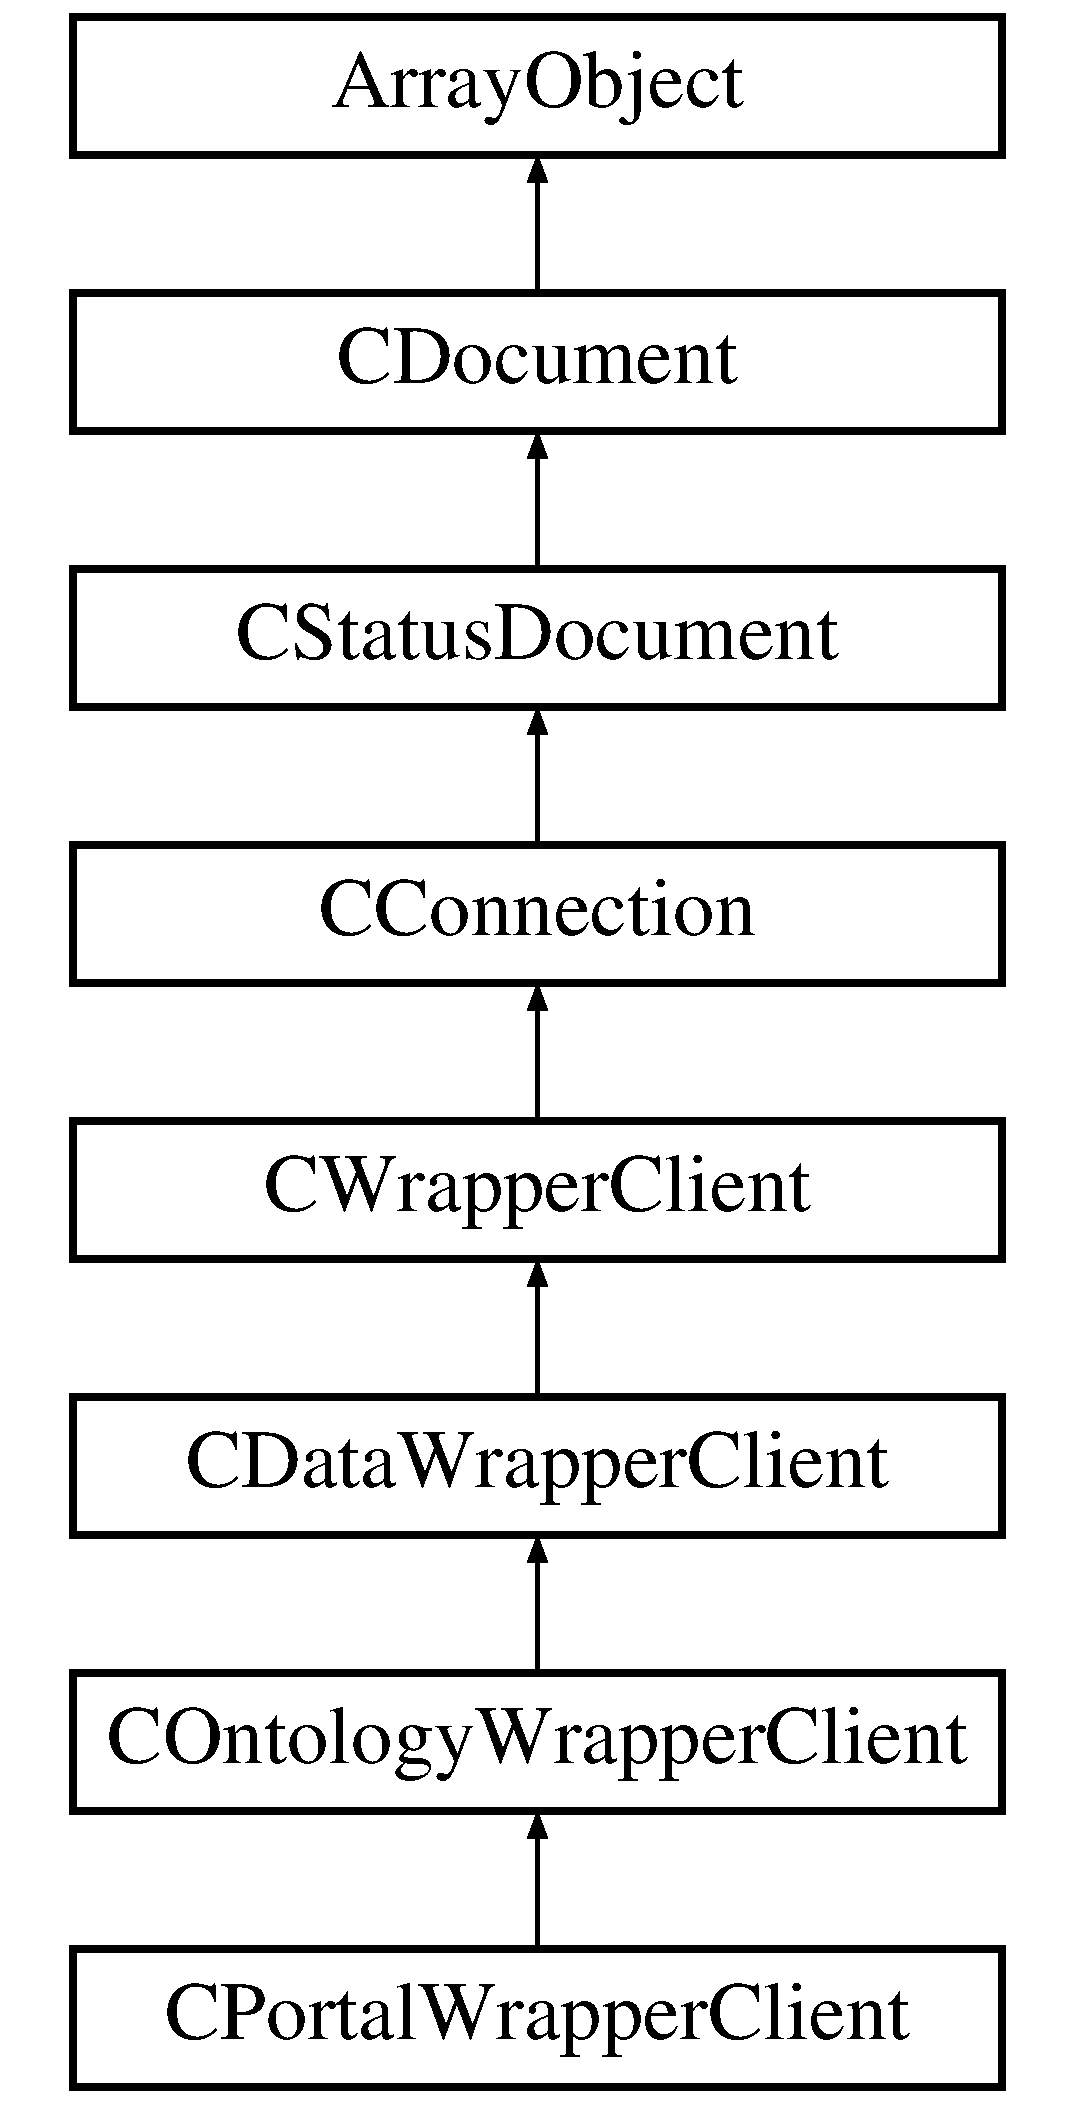
\includegraphics[height=8.000000cm]{class_c_data_wrapper_client}
\end{center}
\end{figure}
\subsection*{Public Member Functions}
\begin{DoxyCompactItemize}
\item 
\hyperlink{class_c_data_wrapper_client_ae7cad4809c20d8f2871cfe00da909d67}{Operation} (\$the\-Value=N\-U\-L\-L, \$get\-Old=F\-A\-L\-S\-E)
\item 
\hyperlink{class_c_data_wrapper_client_a4cdd14b07d74eeb834d2a6052902f176}{Database} (\$the\-Value=N\-U\-L\-L, \$get\-Old=F\-A\-L\-S\-E)
\item 
\hyperlink{class_c_data_wrapper_client_a6a696f83f580186da02093327a84fe4f}{Container} (\$the\-Value=N\-U\-L\-L, \$get\-Old=F\-A\-L\-S\-E)
\item 
\hyperlink{class_c_data_wrapper_client_a4d88af5cdfeb4f4592f3ecbe09284594}{Page\-Start} (\$the\-Value=N\-U\-L\-L, \$get\-Old=F\-A\-L\-S\-E)
\item 
\hyperlink{class_c_data_wrapper_client_a77fe02364cc6ebb8c8acc699bb373b98}{Page\-Limit} (\$the\-Value=N\-U\-L\-L, \$get\-Old=F\-A\-L\-S\-E)
\item 
\hyperlink{class_c_data_wrapper_client_a81a5e5f23f729bf167c03e6eee4593ed}{Query} (\$the\-Value=N\-U\-L\-L, \$get\-Old=F\-A\-L\-S\-E)
\item 
\hyperlink{class_c_data_wrapper_client_add9cb305a726062800f13263d9f72031}{Select} (\$the\-Value=N\-U\-L\-L, \$get\-Old=F\-A\-L\-S\-E)
\item 
\hyperlink{class_c_data_wrapper_client_a969efbb268050c30644e955e0a532241}{Sort} (\$the\-Field=N\-U\-L\-L, \$the\-Order=N\-U\-L\-L, \$get\-Old=F\-A\-L\-S\-E)
\item 
\hyperlink{class_c_data_wrapper_client_a6353a8617179b8da4c5dbe76f6247c73}{Classname} (\$the\-Value=N\-U\-L\-L, \$get\-Old=F\-A\-L\-S\-E)
\item 
\hyperlink{class_c_data_wrapper_client_ab5a1dd1e3b56468f2748f9e1ecad92fc}{Object} (\$the\-Value=N\-U\-L\-L, \$get\-Old=F\-A\-L\-S\-E)
\item 
\hyperlink{class_c_data_wrapper_client_a5a4050c5183d5b9ad07216d67b36d638}{Add\-Query\-Statement} (\$the\-Condition, \$the\-Subject, \$the\-Operator, \$the\-Object=N\-U\-L\-L, \$the\-Type=N\-U\-L\-L)
\item 
\hyperlink{class_c_data_wrapper_client_a44e2a7446e4a67d401db9d189eb7a25f}{Add\-Query\-List\-Statement} (\$the\-Index, \$the\-Condition, \$the\-Subject, \$the\-Operator, \$the\-Object=N\-U\-L\-L, \$the\-Type=N\-U\-L\-L)
\end{DoxyCompactItemize}
\subsection*{Protected Member Functions}
\begin{DoxyCompactItemize}
\item 
\hyperlink{class_c_data_wrapper_client_ae35ac930b0fb89aa47815c81c3450799}{\-\_\-\-Check\-Dependencies} (\$the\-Operation)
\item 
\hyperlink{class_c_data_wrapper_client_a566916298b46dbc2258714e9750e3f8f}{\-\_\-\-Normalise\-Parameters} ()
\item 
\hyperlink{class_c_data_wrapper_client_a0b6d0d8775244822122c201281012b3b}{\-\_\-\-Encode\-Parameters} (\&\$the\-Parameters, \$the\-Encoding)
\item 
\hyperlink{class_c_data_wrapper_client_ab8151cede5da2687546ba3df95182410}{\-\_\-\-Query\-Statement} (\$the\-Subject, \$the\-Operator, \$the\-Object=N\-U\-L\-L, \$the\-Type=N\-U\-L\-L)
\end{DoxyCompactItemize}
\subsection*{Additional Inherited Members}


\subsection{Member Function Documentation}
\hypertarget{class_c_data_wrapper_client_ae35ac930b0fb89aa47815c81c3450799}{\index{C\-Data\-Wrapper\-Client@{C\-Data\-Wrapper\-Client}!\-\_\-\-Check\-Dependencies@{\-\_\-\-Check\-Dependencies}}
\index{\-\_\-\-Check\-Dependencies@{\-\_\-\-Check\-Dependencies}!CDataWrapperClient@{C\-Data\-Wrapper\-Client}}
\subsubsection[{\-\_\-\-Check\-Dependencies}]{\setlength{\rightskip}{0pt plus 5cm}C\-Data\-Wrapper\-Client\-::\-\_\-\-Check\-Dependencies (
\begin{DoxyParamCaption}
\item[{}]{\$the\-Operation}
\end{DoxyParamCaption}
)\hspace{0.3cm}{\ttfamily [protected]}}}\label{class_c_data_wrapper_client_ae35ac930b0fb89aa47815c81c3450799}
Check operation dependencies.

This method can be used to assert whether the required parameters are present depending on the requested operation.


\begin{DoxyParams}[1]{Parameters}
string & {\em \$the\-Operation} & Requested operation.\\
\hline
\end{DoxyParams}
protected


\begin{DoxyExceptions}{Exceptions}
{\em Exception} & \\
\hline
\end{DoxyExceptions}
\hypertarget{class_c_data_wrapper_client_a0b6d0d8775244822122c201281012b3b}{\index{C\-Data\-Wrapper\-Client@{C\-Data\-Wrapper\-Client}!\-\_\-\-Encode\-Parameters@{\-\_\-\-Encode\-Parameters}}
\index{\-\_\-\-Encode\-Parameters@{\-\_\-\-Encode\-Parameters}!CDataWrapperClient@{C\-Data\-Wrapper\-Client}}
\subsubsection[{\-\_\-\-Encode\-Parameters}]{\setlength{\rightskip}{0pt plus 5cm}C\-Data\-Wrapper\-Client\-::\-\_\-\-Encode\-Parameters (
\begin{DoxyParamCaption}
\item[{\&}]{\$the\-Parameters, }
\item[{}]{\$the\-Encoding}
\end{DoxyParamCaption}
)\hspace{0.3cm}{\ttfamily [protected]}}}\label{class_c_data_wrapper_client_a0b6d0d8775244822122c201281012b3b}
Encode parameters.

This method can be used to encode parameters before they get sent to the service.

We overload this method to handle the local parameters.


\begin{DoxyParams}[1]{Parameters}
reference & {\em \&\$the\-Parameters} & List of parameters. \\
\hline
string & {\em \$the\-Encoding} & Encoding code.\\
\hline
\end{DoxyParams}
protected \hypertarget{class_c_data_wrapper_client_a566916298b46dbc2258714e9750e3f8f}{\index{C\-Data\-Wrapper\-Client@{C\-Data\-Wrapper\-Client}!\-\_\-\-Normalise\-Parameters@{\-\_\-\-Normalise\-Parameters}}
\index{\-\_\-\-Normalise\-Parameters@{\-\_\-\-Normalise\-Parameters}!CDataWrapperClient@{C\-Data\-Wrapper\-Client}}
\subsubsection[{\-\_\-\-Normalise\-Parameters}]{\setlength{\rightskip}{0pt plus 5cm}C\-Data\-Wrapper\-Client\-::\-\_\-\-Normalise\-Parameters (
\begin{DoxyParamCaption}
{}
\end{DoxyParamCaption}
)\hspace{0.3cm}{\ttfamily [protected]}}}\label{class_c_data_wrapper_client_a566916298b46dbc2258714e9750e3f8f}
Normalise parameters.

This method can be used to normalise parameters before they get encoded.

In this class we set the request time stamp if the current value is not an float.

In derived classes you should call first the parent method, then handle the local parameters.

protected \hypertarget{class_c_data_wrapper_client_ab8151cede5da2687546ba3df95182410}{\index{C\-Data\-Wrapper\-Client@{C\-Data\-Wrapper\-Client}!\-\_\-\-Query\-Statement@{\-\_\-\-Query\-Statement}}
\index{\-\_\-\-Query\-Statement@{\-\_\-\-Query\-Statement}!CDataWrapperClient@{C\-Data\-Wrapper\-Client}}
\subsubsection[{\-\_\-\-Query\-Statement}]{\setlength{\rightskip}{0pt plus 5cm}C\-Data\-Wrapper\-Client\-::\-\_\-\-Query\-Statement (
\begin{DoxyParamCaption}
\item[{}]{\$the\-Subject, }
\item[{}]{\$the\-Operator, }
\item[{}]{\$the\-Object = {\ttfamily NULL}, }
\item[{}]{\$the\-Type = {\ttfamily NULL}}
\end{DoxyParamCaption}
)\hspace{0.3cm}{\ttfamily [protected]}}}\label{class_c_data_wrapper_client_ab8151cede5da2687546ba3df95182410}
Return a query statement.

This method can be used to retrieve a query statement given the provided parameters, see the \hyperlink{class_c_data_wrapper_client_a5a4050c5183d5b9ad07216d67b36d638}{Add\-Query\-Statement()} method for an explanation of the parameters.


\begin{DoxyParams}[1]{Parameters}
mixed & {\em \$the\-Subject} & Statement subject. \\
\hline
string & {\em \$the\-Operator} & Statement operator. \\
\hline
mixed & {\em \$the\-Object} & Statement object. \\
\hline
string & {\em \$the\-Type} & Statement object data type.\\
\hline
\end{DoxyParams}
protected \begin{DoxyReturn}{Returns}
array 
\end{DoxyReturn}
\hypertarget{class_c_data_wrapper_client_a44e2a7446e4a67d401db9d189eb7a25f}{\index{C\-Data\-Wrapper\-Client@{C\-Data\-Wrapper\-Client}!Add\-Query\-List\-Statement@{Add\-Query\-List\-Statement}}
\index{Add\-Query\-List\-Statement@{Add\-Query\-List\-Statement}!CDataWrapperClient@{C\-Data\-Wrapper\-Client}}
\subsubsection[{Add\-Query\-List\-Statement}]{\setlength{\rightskip}{0pt plus 5cm}C\-Data\-Wrapper\-Client\-::\-Add\-Query\-List\-Statement (
\begin{DoxyParamCaption}
\item[{}]{\$the\-Index, }
\item[{}]{\$the\-Condition, }
\item[{}]{\$the\-Subject, }
\item[{}]{\$the\-Operator, }
\item[{}]{\$the\-Object = {\ttfamily NULL}, }
\item[{}]{\$the\-Type = {\ttfamily NULL}}
\end{DoxyParamCaption}
)}}\label{class_c_data_wrapper_client_a44e2a7446e4a67d401db9d189eb7a25f}
Add a query list statement.

This method is similar to the \hyperlink{class_c_data_wrapper_client_a5a4050c5183d5b9ad07216d67b36d638}{Add\-Query\-Statement()} method as it adds a query statement to a query, except that the current \hyperlink{class_c_data_wrapper_client_a81a5e5f23f729bf167c03e6eee4593ed}{Query()} is a list of \hyperlink{class_c_query}{C\-Query} objects. This kind of structure is used by the \hyperlink{}{k\-A\-P\-I\-\_\-\-O\-P\-\_\-\-G\-E\-T} operation to return the first match of a series of queries and by other operations in which the array element index represents the container name (\hyperlink{class_c_data_wrapper_client_a6a696f83f580186da02093327a84fe4f}{Container()}).

The method expects the following parameters\-:


\begin{DoxyItemize}
\item {\ttfamily \$the\-Index}\-: This parameter represents the list index to the query to which the statement is to be appended. This parameter may either represent a generic index, or it may represent the container name to which the query applies. 
\item {\ttfamily \$the\-Condition}\-: The \hyperlink{}{k\-O\-P\-E\-R\-A\-T\-O\-R\-\_\-\-A\-N\-D}, \hyperlink{}{k\-O\-P\-E\-R\-A\-T\-O\-R\-\_\-\-N\-A\-N\-D}, \hyperlink{}{k\-O\-P\-E\-R\-A\-T\-O\-R\-\_\-\-O\-R} or \hyperlink{}{k\-O\-P\-E\-R\-A\-T\-O\-R\-\_\-\-N\-O\-R} operator (see the \hyperlink{}{Operators.\-inc.\-php} source). 
\item {\ttfamily \$the\-Subject}\-: The subject or attribute of the query, it will be the tag \hyperlink{}{k\-T\-A\-G\-\_\-\-N\-I\-D} (see the \hyperlink{}{Operators.\-inc.\-php} source). 
\item {\ttfamily \$the\-Operator}\-: The statement operator or operation. 
\item {\ttfamily \$the\-Object}\-: The object or value of the statement, this parameter may be omitted of the operator does not require it. 
\item {\ttfamily \$the\-Type}\-: The data type of the statement object (see the \hyperlink{}{Types.\-inc.\-php} source). 
\end{DoxyItemize}

Each element of the queries list will be a \hyperlink{class_c_query}{C\-Query} object and converted to an array before being sent to the server.

Note that this method should only be used if the \hyperlink{}{k\-A\-P\-I\-\_\-\-Q\-U\-E\-R\-Y} property of the object refers to a list of queries\-: if the attribute should refer to a scalar query, you should use the \hyperlink{class_c_data_wrapper_client_a5a4050c5183d5b9ad07216d67b36d638}{Add\-Query\-Statement()} method.


\begin{DoxyParams}[1]{Parameters}
string & {\em \$the\-Index} & Query index. \\
\hline
string & {\em \$the\-Condition} & Statement condition. \\
\hline
mixed & {\em \$the\-Subject} & Statement subject. \\
\hline
string & {\em \$the\-Operator} & Statement operator. \\
\hline
mixed & {\em \$the\-Object} & Statement object. \\
\hline
string & {\em \$the\-Type} & Statement object data type.\\
\hline
\end{DoxyParams}
public


\begin{DoxyExceptions}{Exceptions}
{\em Exception} & \\
\hline
\end{DoxyExceptions}
\begin{DoxySeeAlso}{See Also}
k\-A\-P\-I\-\_\-\-Q\-U\-E\-R\-Y 
\end{DoxySeeAlso}
\hypertarget{class_c_data_wrapper_client_a5a4050c5183d5b9ad07216d67b36d638}{\index{C\-Data\-Wrapper\-Client@{C\-Data\-Wrapper\-Client}!Add\-Query\-Statement@{Add\-Query\-Statement}}
\index{Add\-Query\-Statement@{Add\-Query\-Statement}!CDataWrapperClient@{C\-Data\-Wrapper\-Client}}
\subsubsection[{Add\-Query\-Statement}]{\setlength{\rightskip}{0pt plus 5cm}C\-Data\-Wrapper\-Client\-::\-Add\-Query\-Statement (
\begin{DoxyParamCaption}
\item[{}]{\$the\-Condition, }
\item[{}]{\$the\-Subject, }
\item[{}]{\$the\-Operator, }
\item[{}]{\$the\-Object = {\ttfamily NULL}, }
\item[{}]{\$the\-Type = {\ttfamily NULL}}
\end{DoxyParamCaption}
)}}\label{class_c_data_wrapper_client_a5a4050c5183d5b9ad07216d67b36d638}
Add a query statement.

This method can be used to add a query statement to the current query, it expects the query to be a scalar query with thew container provided in the service parameters.

The method expects the following parameters\-:


\begin{DoxyItemize}
\item {\ttfamily \$the\-Condition}\-: The \hyperlink{}{k\-O\-P\-E\-R\-A\-T\-O\-R\-\_\-\-A\-N\-D}, \hyperlink{}{k\-O\-P\-E\-R\-A\-T\-O\-R\-\_\-\-N\-A\-N\-D}, \hyperlink{}{k\-O\-P\-E\-R\-A\-T\-O\-R\-\_\-\-O\-R} or \hyperlink{}{k\-O\-P\-E\-R\-A\-T\-O\-R\-\_\-\-N\-O\-R} operator (see the \hyperlink{}{Operators.\-inc.\-php} source). 
\item {\ttfamily \$the\-Subject}\-: The subject or attribute of the query, it will be the tag \hyperlink{}{k\-T\-A\-G\-\_\-\-N\-I\-D} (see the \hyperlink{}{Operators.\-inc.\-php} source). 
\item {\ttfamily \$the\-Operator}\-: The statement operator or operation. 
\item {\ttfamily \$the\-Object}\-: The object or value of the statement, this parameter may be omitted of the operator does not require it. 
\item {\ttfamily \$the\-Type}\-: The data type of the statement object (see the \hyperlink{}{Types.\-inc.\-php} source). 
\end{DoxyItemize}

The query attribute will be set as a \hyperlink{class_c_query}{C\-Query} object and converted to an array before being sent to the server.

Note that this method should only be used if the \hyperlink{}{k\-A\-P\-I\-\_\-\-Q\-U\-E\-R\-Y} property of the object refers to a single query\-: if the attribute should refer to a list of queries, you should use the \hyperlink{class_c_data_wrapper_client_a44e2a7446e4a67d401db9d189eb7a25f}{Add\-Query\-List\-Statement()} method.


\begin{DoxyParams}[1]{Parameters}
string & {\em \$the\-Condition} & Statement condition. \\
\hline
mixed & {\em \$the\-Subject} & Statement subject. \\
\hline
string & {\em \$the\-Operator} & Statement operator. \\
\hline
mixed & {\em \$the\-Object} & Statement object. \\
\hline
string & {\em \$the\-Type} & Statement object data type.\\
\hline
\end{DoxyParams}
public


\begin{DoxyExceptions}{Exceptions}
{\em Exception} & \\
\hline
\end{DoxyExceptions}
\begin{DoxySeeAlso}{See Also}
k\-A\-P\-I\-\_\-\-Q\-U\-E\-R\-Y 
\end{DoxySeeAlso}
\hypertarget{class_c_data_wrapper_client_a6353a8617179b8da4c5dbe76f6247c73}{\index{C\-Data\-Wrapper\-Client@{C\-Data\-Wrapper\-Client}!Classname@{Classname}}
\index{Classname@{Classname}!CDataWrapperClient@{C\-Data\-Wrapper\-Client}}
\subsubsection[{Classname}]{\setlength{\rightskip}{0pt plus 5cm}C\-Data\-Wrapper\-Client\-::\-Classname (
\begin{DoxyParamCaption}
\item[{}]{\$the\-Value = {\ttfamily NULL}, }
\item[{}]{\$get\-Old = {\ttfamily FALSE}}
\end{DoxyParamCaption}
)}}\label{class_c_data_wrapper_client_a6353a8617179b8da4c5dbe76f6247c73}
Manage object class.

This method can be used to manage the \hyperlink{}{k\-A\-P\-I\-\_\-\-C\-L\-A\-S\-S} offset, it accepts a string parameter which represents the class name of the object provided in \hyperlink{class_c_data_wrapper_client_ab5a1dd1e3b56468f2748f9e1ecad92fc}{Object()} or the requested operation, depending on its value\-:


\begin{DoxyItemize}
\item {\itshape N\-U\-L\-L}\-: Return the current value. 
\item {\itshape F\-A\-L\-S\-E}\-: Delete the current value. 
\item {\itshape other}\-: Set the value with the provided parameter, in this case the value is expected to be and will be casted to an integer. 
\end{DoxyItemize}

The second parameter is a boolean which if {\itshape T\-R\-U\-E} will return the {\itshape old} value when replacing values; if {\itshape F\-A\-L\-S\-E}, it will return the currently set value.


\begin{DoxyParams}[1]{Parameters}
string & {\em \$the\-Value} & Value or operation. \\
\hline
boolean & {\em \$get\-Old} & T\-R\-U\-E get old value.\\
\hline
\end{DoxyParams}
public \begin{DoxyReturn}{Returns}
mixed
\end{DoxyReturn}
Manage\-Offset()

\begin{DoxySeeAlso}{See Also}
k\-A\-P\-I\-\_\-\-C\-L\-A\-S\-S 
\end{DoxySeeAlso}
\hypertarget{class_c_data_wrapper_client_a6a696f83f580186da02093327a84fe4f}{\index{C\-Data\-Wrapper\-Client@{C\-Data\-Wrapper\-Client}!Container@{Container}}
\index{Container@{Container}!CDataWrapperClient@{C\-Data\-Wrapper\-Client}}
\subsubsection[{Container}]{\setlength{\rightskip}{0pt plus 5cm}C\-Data\-Wrapper\-Client\-::\-Container (
\begin{DoxyParamCaption}
\item[{}]{\$the\-Value = {\ttfamily NULL}, }
\item[{}]{\$get\-Old = {\ttfamily FALSE}}
\end{DoxyParamCaption}
)}}\label{class_c_data_wrapper_client_a6a696f83f580186da02093327a84fe4f}
Manage container name.

This method can be used to manage the \hyperlink{}{k\-A\-P\-I\-\_\-\-C\-O\-N\-T\-A\-I\-N\-E\-R} offset, it accepts a parameter which represents the container name or the requested operation, depending on its value\-:


\begin{DoxyItemize}
\item {\itshape N\-U\-L\-L}\-: Return the current value. 
\item {\itshape F\-A\-L\-S\-E}\-: Delete the current value. 
\item {\itshape other}\-: Set the value with the provided parameter. 
\end{DoxyItemize}

The second parameter is a boolean which if {\itshape T\-R\-U\-E} will return the {\itshape old} value when replacing values; if {\itshape F\-A\-L\-S\-E}, it will return the currently set value.


\begin{DoxyParams}[1]{Parameters}
string & {\em \$the\-Value} & Value or operation. \\
\hline
boolean & {\em \$get\-Old} & T\-R\-U\-E get old value.\\
\hline
\end{DoxyParams}
public \begin{DoxyReturn}{Returns}
mixed
\end{DoxyReturn}
Manage\-Offset()

\begin{DoxySeeAlso}{See Also}
k\-A\-P\-I\-\_\-\-C\-O\-N\-T\-A\-I\-N\-E\-R 
\end{DoxySeeAlso}
\hypertarget{class_c_data_wrapper_client_a4cdd14b07d74eeb834d2a6052902f176}{\index{C\-Data\-Wrapper\-Client@{C\-Data\-Wrapper\-Client}!Database@{Database}}
\index{Database@{Database}!CDataWrapperClient@{C\-Data\-Wrapper\-Client}}
\subsubsection[{Database}]{\setlength{\rightskip}{0pt plus 5cm}C\-Data\-Wrapper\-Client\-::\-Database (
\begin{DoxyParamCaption}
\item[{}]{\$the\-Value = {\ttfamily NULL}, }
\item[{}]{\$get\-Old = {\ttfamily FALSE}}
\end{DoxyParamCaption}
)}}\label{class_c_data_wrapper_client_a4cdd14b07d74eeb834d2a6052902f176}
Manage database name.

This method can be used to manage the \hyperlink{}{k\-A\-P\-I\-\_\-\-D\-A\-T\-A\-B\-A\-S\-E} offset, it accepts a parameter which represents the database name or the requested operation, depending on its value\-:


\begin{DoxyItemize}
\item {\itshape N\-U\-L\-L}\-: Return the current value. 
\item {\itshape F\-A\-L\-S\-E}\-: Delete the current value. 
\item {\itshape other}\-: Set the value with the provided parameter. 
\end{DoxyItemize}

The second parameter is a boolean which if {\itshape T\-R\-U\-E} will return the {\itshape old} value when replacing values; if {\itshape F\-A\-L\-S\-E}, it will return the currently set value.


\begin{DoxyParams}[1]{Parameters}
string & {\em \$the\-Value} & Value or operation. \\
\hline
boolean & {\em \$get\-Old} & T\-R\-U\-E get old value.\\
\hline
\end{DoxyParams}
public \begin{DoxyReturn}{Returns}
mixed
\end{DoxyReturn}
Manage\-Offset()

\begin{DoxySeeAlso}{See Also}
k\-A\-P\-I\-\_\-\-D\-A\-T\-A\-B\-A\-S\-E 
\end{DoxySeeAlso}
\hypertarget{class_c_data_wrapper_client_ab5a1dd1e3b56468f2748f9e1ecad92fc}{\index{C\-Data\-Wrapper\-Client@{C\-Data\-Wrapper\-Client}!Object@{Object}}
\index{Object@{Object}!CDataWrapperClient@{C\-Data\-Wrapper\-Client}}
\subsubsection[{Object}]{\setlength{\rightskip}{0pt plus 5cm}C\-Data\-Wrapper\-Client\-::\-Object (
\begin{DoxyParamCaption}
\item[{}]{\$the\-Value = {\ttfamily NULL}, }
\item[{}]{\$get\-Old = {\ttfamily FALSE}}
\end{DoxyParamCaption}
)}}\label{class_c_data_wrapper_client_ab5a1dd1e3b56468f2748f9e1ecad92fc}
Manage object.

This method can be used to manage the \hyperlink{}{k\-A\-P\-I\-\_\-\-O\-B\-J\-E\-C\-T} offset, it accepts a parameter which represents either the object to be inserted or the value used to resolve the object to be deleted, or the requested operation, depending on its value\-:


\begin{DoxyItemize}
\item {\itshape N\-U\-L\-L}\-: Return the current value. 
\item {\itshape F\-A\-L\-S\-E}\-: Delete the current value. 
\item {\itshape other}\-: Set the value with the provided parameter, in this case the value is expected to be and will be casted to an integer. 
\end{DoxyItemize}

The second parameter is a boolean which if {\itshape T\-R\-U\-E} will return the {\itshape old} value when replacing values; if {\itshape F\-A\-L\-S\-E}, it will return the currently set value.

{\itshape Note that if you provide an object derived from \hyperlink{class_c_persistent_object}{C\-Persistent\-Object}, this method will also set automatically the \hyperlink{class_c_data_wrapper_client_a6353a8617179b8da4c5dbe76f6247c73}{Classname()} parameter.}


\begin{DoxyParams}[1]{Parameters}
string & {\em \$the\-Value} & Value or operation. \\
\hline
boolean & {\em \$get\-Old} & T\-R\-U\-E get old value.\\
\hline
\end{DoxyParams}
public \begin{DoxyReturn}{Returns}
mixed
\end{DoxyReturn}
Manage\-Offset()

\begin{DoxySeeAlso}{See Also}
k\-A\-P\-I\-\_\-\-O\-B\-J\-E\-C\-T 
\end{DoxySeeAlso}
\hypertarget{class_c_data_wrapper_client_ae7cad4809c20d8f2871cfe00da909d67}{\index{C\-Data\-Wrapper\-Client@{C\-Data\-Wrapper\-Client}!Operation@{Operation}}
\index{Operation@{Operation}!CDataWrapperClient@{C\-Data\-Wrapper\-Client}}
\subsubsection[{Operation}]{\setlength{\rightskip}{0pt plus 5cm}C\-Data\-Wrapper\-Client\-::\-Operation (
\begin{DoxyParamCaption}
\item[{}]{\$the\-Value = {\ttfamily NULL}, }
\item[{}]{\$get\-Old = {\ttfamily FALSE}}
\end{DoxyParamCaption}
)}}\label{class_c_data_wrapper_client_ae7cad4809c20d8f2871cfe00da909d67}
Manage operation.

We \hyperlink{class_c_wrapper_client_ae378229fd57b051ddf0e0a7abf599641}{overload} this method to add the following allowed operations\-:


\begin{DoxyItemize}
\item {\itshape \hyperlink{}{k\-A\-P\-I\-\_\-\-O\-P\-\_\-\-C\-O\-U\-N\-T}}\-: C\-O\-U\-N\-T web-\/service operation, used to return the total number of elements satisfying a query. 
\item {\itshape \hyperlink{}{k\-A\-P\-I\-\_\-\-O\-P\-\_\-\-G\-E\-T}}\-: G\-E\-T web-\/service operation, used to retrieve objects from the data store. 
\item {\itshape \hyperlink{}{k\-A\-P\-I\-\_\-\-O\-P\-\_\-\-S\-E\-T}}\-: S\-E\-T web-\/service operation, used to insert or update objects in the data store. 
\item {\itshape \hyperlink{}{k\-A\-P\-I\-\_\-\-O\-P\-\_\-\-U\-P\-D\-A\-T\-E}}\-: U\-P\-D\-A\-T\-E web-\/service operation, used to update existing objects in the data store. 
\item {\itshape \hyperlink{}{k\-A\-P\-I\-\_\-\-O\-P\-\_\-\-I\-N\-S\-E\-R\-T}}\-: I\-N\-S\-E\-R\-T web-\/service operation, used to insert new objects in the data store. 
\end{DoxyItemize}


\begin{DoxyParams}[1]{Parameters}
string & {\em \$the\-Value} & Value or operation. \\
\hline
boolean & {\em \$get\-Old} & T\-R\-U\-E get old value.\\
\hline
\end{DoxyParams}
public \begin{DoxyReturn}{Returns}
mixed
\end{DoxyReturn}

\begin{DoxyExceptions}{Exceptions}
{\em \{@link} & \hyperlink{class_c_exception}{C\-Exception} \hyperlink{class_c_exception}{C\-Exception}\}\\
\hline
\end{DoxyExceptions}
C\-Attribute\-::\-Manage\-Offset()

\begin{DoxySeeAlso}{See Also}
k\-A\-P\-I\-\_\-\-O\-P\-E\-R\-A\-T\-I\-O\-N 

k\-A\-P\-I\-\_\-\-O\-P\-\_\-\-H\-E\-L\-P k\-A\-P\-I\-\_\-\-O\-P\-\_\-\-P\-I\-N\-G 
\end{DoxySeeAlso}
\hypertarget{class_c_data_wrapper_client_a77fe02364cc6ebb8c8acc699bb373b98}{\index{C\-Data\-Wrapper\-Client@{C\-Data\-Wrapper\-Client}!Page\-Limit@{Page\-Limit}}
\index{Page\-Limit@{Page\-Limit}!CDataWrapperClient@{C\-Data\-Wrapper\-Client}}
\subsubsection[{Page\-Limit}]{\setlength{\rightskip}{0pt plus 5cm}C\-Data\-Wrapper\-Client\-::\-Page\-Limit (
\begin{DoxyParamCaption}
\item[{}]{\$the\-Value = {\ttfamily NULL}, }
\item[{}]{\$get\-Old = {\ttfamily FALSE}}
\end{DoxyParamCaption}
)}}\label{class_c_data_wrapper_client_a77fe02364cc6ebb8c8acc699bb373b98}
Manage page limit.

This method can be used to manage the \hyperlink{}{k\-A\-P\-I\-\_\-\-P\-A\-G\-E\-\_\-\-L\-I\-M\-I\-T} offset, it accepts a parameter which represents the maximum number of elements to be returned by the service, or the requested operation, depending on its value\-:


\begin{DoxyItemize}
\item {\itshape N\-U\-L\-L}\-: Return the current value. 
\item {\itshape F\-A\-L\-S\-E}\-: Delete the current value. 
\item {\itshape other}\-: Set the value with the provided parameter, in this case the value is expected to be and will be casted to an integer. 
\end{DoxyItemize}

The second parameter is a boolean which if {\itshape T\-R\-U\-E} will return the {\itshape old} value when replacing values; if {\itshape F\-A\-L\-S\-E}, it will return the currently set value.


\begin{DoxyParams}[1]{Parameters}
string & {\em \$the\-Value} & Value or operation. \\
\hline
boolean & {\em \$get\-Old} & T\-R\-U\-E get old value.\\
\hline
\end{DoxyParams}
public \begin{DoxyReturn}{Returns}
mixed
\end{DoxyReturn}
Manage\-Offset()

\begin{DoxySeeAlso}{See Also}
k\-A\-P\-I\-\_\-\-P\-A\-G\-E\-\_\-\-L\-I\-M\-I\-T 
\end{DoxySeeAlso}
\hypertarget{class_c_data_wrapper_client_a4d88af5cdfeb4f4592f3ecbe09284594}{\index{C\-Data\-Wrapper\-Client@{C\-Data\-Wrapper\-Client}!Page\-Start@{Page\-Start}}
\index{Page\-Start@{Page\-Start}!CDataWrapperClient@{C\-Data\-Wrapper\-Client}}
\subsubsection[{Page\-Start}]{\setlength{\rightskip}{0pt plus 5cm}C\-Data\-Wrapper\-Client\-::\-Page\-Start (
\begin{DoxyParamCaption}
\item[{}]{\$the\-Value = {\ttfamily NULL}, }
\item[{}]{\$get\-Old = {\ttfamily FALSE}}
\end{DoxyParamCaption}
)}}\label{class_c_data_wrapper_client_a4d88af5cdfeb4f4592f3ecbe09284594}
Manage page start.

This method can be used to manage the \hyperlink{}{k\-A\-P\-I\-\_\-\-P\-A\-G\-E\-\_\-\-S\-T\-A\-R\-T} offset, it accepts a parameter which represents the starting page from which the service should return data, or the requested operation, depending on its value\-:


\begin{DoxyItemize}
\item {\itshape N\-U\-L\-L}\-: Return the current value. 
\item {\itshape F\-A\-L\-S\-E}\-: Delete the current value. 
\item {\itshape other}\-: Set the value with the provided parameter, in this case the value is expected to be and will be casted to an integer. 
\end{DoxyItemize}

The second parameter is a boolean which if {\itshape T\-R\-U\-E} will return the {\itshape old} value when replacing values; if {\itshape F\-A\-L\-S\-E}, it will return the currently set value.


\begin{DoxyParams}[1]{Parameters}
string & {\em \$the\-Value} & Value or operation. \\
\hline
boolean & {\em \$get\-Old} & T\-R\-U\-E get old value.\\
\hline
\end{DoxyParams}
public \begin{DoxyReturn}{Returns}
mixed
\end{DoxyReturn}
Manage\-Offset()

\begin{DoxySeeAlso}{See Also}
k\-A\-P\-I\-\_\-\-P\-A\-G\-E\-\_\-\-S\-T\-A\-R\-T 
\end{DoxySeeAlso}
\hypertarget{class_c_data_wrapper_client_a81a5e5f23f729bf167c03e6eee4593ed}{\index{C\-Data\-Wrapper\-Client@{C\-Data\-Wrapper\-Client}!Query@{Query}}
\index{Query@{Query}!CDataWrapperClient@{C\-Data\-Wrapper\-Client}}
\subsubsection[{Query}]{\setlength{\rightskip}{0pt plus 5cm}C\-Data\-Wrapper\-Client\-::\-Query (
\begin{DoxyParamCaption}
\item[{}]{\$the\-Value = {\ttfamily NULL}, }
\item[{}]{\$get\-Old = {\ttfamily FALSE}}
\end{DoxyParamCaption}
)}}\label{class_c_data_wrapper_client_a81a5e5f23f729bf167c03e6eee4593ed}
Manage query.

This method can be used to manage the \hyperlink{}{k\-A\-P\-I\-\_\-\-Q\-U\-E\-R\-Y} offset, it accepts a parameter which represents the service requested query, or the requested operation, depending on its value\-:


\begin{DoxyItemize}
\item {\itshape N\-U\-L\-L}\-: Return the current value. 
\item {\itshape F\-A\-L\-S\-E}\-: Delete the current value. 
\item {\itshape other}\-: Set the value with the provided parameter, in this case the value is expected to be\-: 
\begin{DoxyItemize}
\item {\ttfamily array} or {\ttfamily Array\-Object{\ttfamily \-: The provided array will be cast to a \hyperlink{class_c_query}{C\-Query} object and verified. }}
\item {\ttfamily {\ttfamily {\ttfamily \hyperlink{class_c_query}{C\-Query}}\-: The provided array will be verified. }}
\item {\ttfamily {\ttfamily {\itshape other}\-: The method will raise an exception. }}
\end{DoxyItemize}
\end{DoxyItemize}

{\ttfamily {\ttfamily The second parameter is a boolean which if {\itshape T\-R\-U\-E} will return the {\itshape old} value when replacing values; if {\itshape F\-A\-L\-S\-E}, it will return the currently set value.}}

{\ttfamily {\ttfamily 
\begin{DoxyParams}[1]{Parameters}
string & {\em \$the\-Value} & Value or operation. \\
\hline
boolean & {\em \$get\-Old} & T\-R\-U\-E get old value.\\
\hline
\end{DoxyParams}
public \begin{DoxyReturn}{Returns}
mixed
\end{DoxyReturn}

\begin{DoxyExceptions}{Exceptions}
{\em Exception} & Manage\-Offset()\\
\hline
\end{DoxyExceptions}
\begin{DoxySeeAlso}{See Also}
k\-A\-P\-I\-\_\-\-Q\-U\-E\-R\-Y 
\end{DoxySeeAlso}
}}\hypertarget{class_c_data_wrapper_client_add9cb305a726062800f13263d9f72031}{\index{C\-Data\-Wrapper\-Client@{C\-Data\-Wrapper\-Client}!Select@{Select}}
\index{Select@{Select}!CDataWrapperClient@{C\-Data\-Wrapper\-Client}}
\subsubsection[{Select}]{\setlength{\rightskip}{0pt plus 5cm}C\-Data\-Wrapper\-Client\-::\-Select (
\begin{DoxyParamCaption}
\item[{}]{\$the\-Value = {\ttfamily NULL}, }
\item[{}]{\$get\-Old = {\ttfamily FALSE}}
\end{DoxyParamCaption}
)}}\label{class_c_data_wrapper_client_add9cb305a726062800f13263d9f72031}
Manage select fields.

This method can be used to manage the \hyperlink{}{k\-A\-P\-I\-\_\-\-S\-E\-L\-E\-C\-T} offset, it accepts a parameter which represents the list of requested attributes, or the requested operation, depending on its value\-:


\begin{DoxyItemize}
\item {\itshape N\-U\-L\-L}\-: Return the current value. 
\item {\itshape F\-A\-L\-S\-E}\-: Delete the current value. 
\item {\itshape other}\-: Set the value with the provided parameter, in this case the value is expected to be\-: 
\begin{DoxyItemize}
\item {\ttfamily array} or {\ttfamily Array\-Object{\ttfamily \-: The provided parameter will become the new list. }}
\item {\ttfamily {\ttfamily {\itshape other}\-: The method will assume the parameter is a string and it will add it to the current list or create a list if it doesn't exist. }}
\end{DoxyItemize}
\end{DoxyItemize}

{\ttfamily {\ttfamily The second parameter is a boolean which if {\itshape T\-R\-U\-E} will return the {\itshape old} value when replacing values; if {\itshape F\-A\-L\-S\-E}, it will return the currently set value.}}

{\ttfamily {\ttfamily 
\begin{DoxyParams}[1]{Parameters}
string & {\em \$the\-Value} & Value or operation. \\
\hline
boolean & {\em \$get\-Old} & T\-R\-U\-E get old value.\\
\hline
\end{DoxyParams}
public \begin{DoxyReturn}{Returns}
mixed
\end{DoxyReturn}
\hyperlink{class_c_wrapper_client_a8ad42378b7abfeaaaa311e1b96a42a26}{\-\_\-\-Manage\-List\-Offset()}}}

{\ttfamily {\ttfamily \begin{DoxySeeAlso}{See Also}
k\-A\-P\-I\-\_\-\-S\-E\-L\-E\-C\-T 
\end{DoxySeeAlso}
}}\hypertarget{class_c_data_wrapper_client_a969efbb268050c30644e955e0a532241}{\index{C\-Data\-Wrapper\-Client@{C\-Data\-Wrapper\-Client}!Sort@{Sort}}
\index{Sort@{Sort}!CDataWrapperClient@{C\-Data\-Wrapper\-Client}}
\subsubsection[{Sort}]{\setlength{\rightskip}{0pt plus 5cm}C\-Data\-Wrapper\-Client\-::\-Sort (
\begin{DoxyParamCaption}
\item[{}]{\$the\-Field = {\ttfamily NULL}, }
\item[{}]{\$the\-Order = {\ttfamily NULL}, }
\item[{}]{\$get\-Old = {\ttfamily FALSE}}
\end{DoxyParamCaption}
)}}\label{class_c_data_wrapper_client_a969efbb268050c30644e955e0a532241}
Manage sort fields.

This method can be used to manage the \hyperlink{}{k\-A\-P\-I\-\_\-\-S\-O\-R\-T} offset, the managed value is an array in which the key represents the attribute name and the value is an integer which determines the sort order\-: positive means ascending, negative means descending; zero is ignored.


\begin{DoxyItemize}
\item {\ttfamily \$the\-Field}\-: The field name or list\-: 
\begin{DoxyItemize}
\item {\ttfamily array}\-: If you provide an array in this field, the method will assume you are providing a full list, in this case the method will set the offset with that value, {\itshape without checking its contents}. 
\item {\ttfamily N\-U\-L\-L}\-: Selects all fields. 
\item {\itshape other}\-: Any other value will be interpreted as the field name. 
\end{DoxyItemize}
\item {\ttfamily \$the\-Order}\-: The the sort order\-: 
\begin{DoxyItemize}
\item {\ttfamily N\-U\-L\-L}\-: Return the sort order of the provided field. If the provided field is an array, this parameter will be ignored; if the provided field is a scalar, the method will return the element matching the provided field; if the provided field is {\ttfamily N\-U\-L\-L}, the method will return the full list. 
\item {\ttfamily F\-A\-L\-S\-E}\-: Delete the element matching the provided field\-: if the provided field is an array, this parameter will be ignored; if the provided field is a scalar, the method will delete the element matching the provided field; if the provided field is {\ttfamily N\-U\-L\-L}, the method will return the full list. 
\item {\ttfamily integer}\-: Set the sort order, negative values mean descending; positive values mean ascending. If the provided field is an array, this parameter will be ignored; if the provided field is a scalar, the method will set the element matching the provided field; if the provided field is {\ttfamily N\-U\-L\-L}, the method will set all the elements of the list to the provided sort order. 
\item {\ttfamily zero}\-: If the parameter evaluates to zero, the operation will do nothing. 
\item {\itshape other}\-: Any other type will be cast to an integer. 
\end{DoxyItemize}
\item {\ttfamily \$get\-Old}\-: This parameter is a boolean which if {\itshape T\-R\-U\-E} will return the {\itshape old} value when replacing values; if {\itshape F\-A\-L\-S\-E}, it will return the currently set value. 
\end{DoxyItemize}


\begin{DoxyParams}[1]{Parameters}
string & {\em \$the\-Field} & Field name or fields list. \\
\hline
mixed & {\em \$the\-Order} & Sort order or operation. \\
\hline
boolean & {\em \$get\-Old} & T\-R\-U\-E get old value.\\
\hline
\end{DoxyParams}
public \begin{DoxyReturn}{Returns}
mixed
\end{DoxyReturn}
Manage\-Offset()

\begin{DoxySeeAlso}{See Also}
k\-A\-P\-I\-\_\-\-S\-O\-R\-T 
\end{DoxySeeAlso}


The documentation for this class was generated from the following file\-:\begin{DoxyCompactItemize}
\item 
/\-Library/\-Web\-Server/\-Library/\-P\-H\-P\-Wrapper/classes/C\-Data\-Wrapper\-Client.\-php\end{DoxyCompactItemize}

\hypertarget{class_c_document}{\section{C\-Document Class Reference}
\label{class_c_document}\index{C\-Document@{C\-Document}}
}
Inheritance diagram for C\-Document\-:\begin{figure}[H]
\begin{center}
\leavevmode
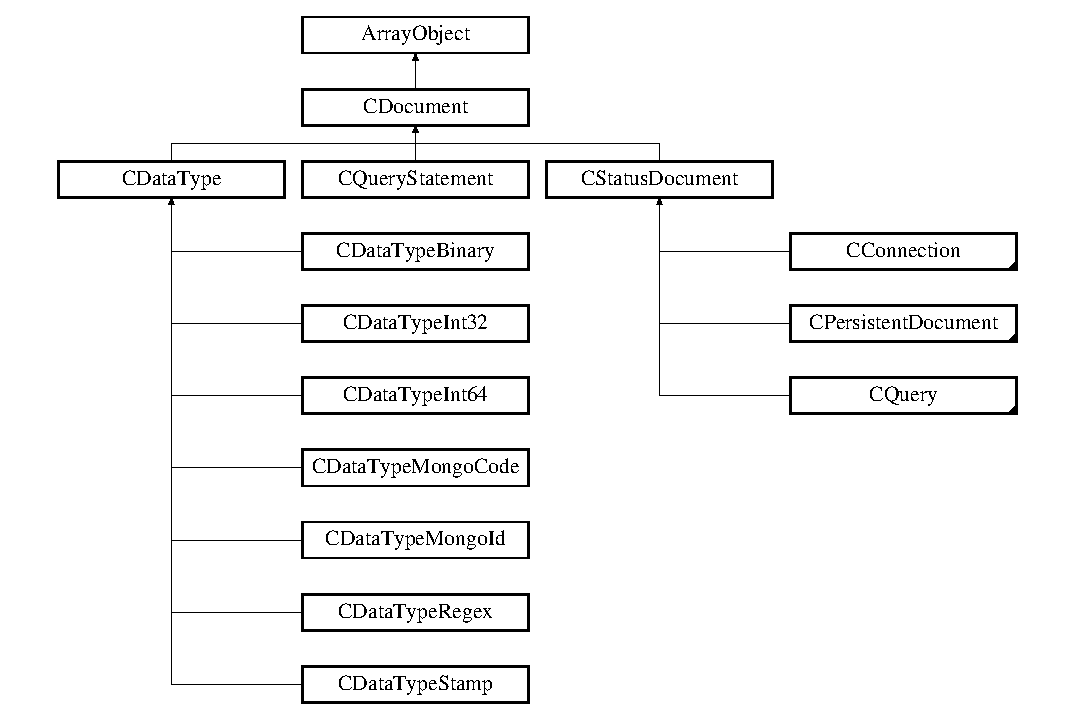
\includegraphics[height=9.210526cm]{class_c_document}
\end{center}
\end{figure}
\subsection*{Public Member Functions}
\begin{DoxyCompactItemize}
\item 
\hyperlink{class_c_document_a7e03e4fd9674ba52b26589d01ca42027}{offset\-Get} (\$the\-Offset)
\item 
\hyperlink{class_c_document_a0fe390a5ce89bc8dd12062276b53154b}{offset\-Set} (\$the\-Offset, \$the\-Value)
\item 
\hyperlink{class_c_document_a1d4b8ba2553520c323edcde52a4113e3}{offset\-Unset} (\$the\-Offset)
\item 
\hyperlink{class_c_document_a1809f3de22bc07e0c57d2ceb0b951ce0}{array\-\_\-keys} ()
\item 
\hyperlink{class_c_document_a82d9b209627c76363fec8c879e4e6225}{array\-\_\-values} ()
\end{DoxyCompactItemize}


\subsection{Member Function Documentation}
\hypertarget{class_c_document_a1809f3de22bc07e0c57d2ceb0b951ce0}{\index{C\-Document@{C\-Document}!array\-\_\-keys@{array\-\_\-keys}}
\index{array\-\_\-keys@{array\-\_\-keys}!CDocument@{C\-Document}}
\subsubsection[{array\-\_\-keys}]{\setlength{\rightskip}{0pt plus 5cm}C\-Document\-::array\-\_\-keys (
\begin{DoxyParamCaption}
{}
\end{DoxyParamCaption}
)}}\label{class_c_document_a1809f3de22bc07e0c57d2ceb0b951ce0}
\subparagraph*{Return object's offsets}

This method has the same function as the P\-H\-P function {\ttfamily \hyperlink{class_c_document_a1809f3de22bc07e0c57d2ceb0b951ce0}{array\-\_\-keys()}, it will return an array comprised of all object's offsets.}

{\ttfamily  public \begin{DoxyReturn}{Returns}
array List of object offsets. 
\end{DoxyReturn}
}\hypertarget{class_c_document_a82d9b209627c76363fec8c879e4e6225}{\index{C\-Document@{C\-Document}!array\-\_\-values@{array\-\_\-values}}
\index{array\-\_\-values@{array\-\_\-values}!CDocument@{C\-Document}}
\subsubsection[{array\-\_\-values}]{\setlength{\rightskip}{0pt plus 5cm}C\-Document\-::array\-\_\-values (
\begin{DoxyParamCaption}
{}
\end{DoxyParamCaption}
)}}\label{class_c_document_a82d9b209627c76363fec8c879e4e6225}
\subparagraph*{Return object's offset values}

This method has the same function as the P\-H\-P function {\ttfamily \hyperlink{class_c_document_a82d9b209627c76363fec8c879e4e6225}{array\-\_\-values()}, it will return an array comprised of all object's offset values.}

{\ttfamily  public \begin{DoxyReturn}{Returns}
array List of object offset values. 
\end{DoxyReturn}
}\hypertarget{class_c_document_a7e03e4fd9674ba52b26589d01ca42027}{\index{C\-Document@{C\-Document}!offset\-Get@{offset\-Get}}
\index{offset\-Get@{offset\-Get}!CDocument@{C\-Document}}
\subsubsection[{offset\-Get}]{\setlength{\rightskip}{0pt plus 5cm}C\-Document\-::offset\-Get (
\begin{DoxyParamCaption}
\item[{}]{\$the\-Offset}
\end{DoxyParamCaption}
)}}\label{class_c_document_a7e03e4fd9674ba52b26589d01ca42027}
\subparagraph*{Return a value at a given offset}

This method should return the value corresponding to the provided offset.

This method is overloaded to prevent notices from being triggered when seeking non-\/existing offsets.

In this class no offset may have a {\ttfamily N\-U\-L\-L} value, if this method returns a {\ttfamily N\-U\-L\-L} value, it means that the offset doesn't exist.


\begin{DoxyParams}[1]{Parameters}
string & {\em \$the\-Offset} & Offset.\\
\hline
\end{DoxyParams}
public \begin{DoxyReturn}{Returns}
mixed Offset value. 
\end{DoxyReturn}
\hypertarget{class_c_document_a0fe390a5ce89bc8dd12062276b53154b}{\index{C\-Document@{C\-Document}!offset\-Set@{offset\-Set}}
\index{offset\-Set@{offset\-Set}!CDocument@{C\-Document}}
\subsubsection[{offset\-Set}]{\setlength{\rightskip}{0pt plus 5cm}C\-Document\-::offset\-Set (
\begin{DoxyParamCaption}
\item[{}]{\$the\-Offset, }
\item[{}]{\$the\-Value}
\end{DoxyParamCaption}
)}}\label{class_c_document_a0fe390a5ce89bc8dd12062276b53154b}
\subparagraph*{Set a value at a given offset}

This method should set the provided value corresponding to the provided offset.

This method is overloaded to prevent setting {\ttfamily N\-U\-L\-L} values\-: if this is the case, the method will unset the offset.


\begin{DoxyParams}[1]{Parameters}
string & {\em \$the\-Offset} & Offset. \\
\hline
mixed & {\em \$the\-Value} & Value to set at offset.\\
\hline
\end{DoxyParams}
public

\hyperlink{class_c_document_a1d4b8ba2553520c323edcde52a4113e3}{offset\-Unset()} \hypertarget{class_c_document_a1d4b8ba2553520c323edcde52a4113e3}{\index{C\-Document@{C\-Document}!offset\-Unset@{offset\-Unset}}
\index{offset\-Unset@{offset\-Unset}!CDocument@{C\-Document}}
\subsubsection[{offset\-Unset}]{\setlength{\rightskip}{0pt plus 5cm}C\-Document\-::offset\-Unset (
\begin{DoxyParamCaption}
\item[{}]{\$the\-Offset}
\end{DoxyParamCaption}
)}}\label{class_c_document_a1d4b8ba2553520c323edcde52a4113e3}
\subparagraph*{Reset a value at a given offset}

This method should reset the value corresponding to the provided offset.

We overload this method to prevent notices on non-\/existing offsets.


\begin{DoxyParams}[1]{Parameters}
string & {\em \$the\-Offset} & Offset.\\
\hline
\end{DoxyParams}
public 

The documentation for this class was generated from the following file\-:\begin{DoxyCompactItemize}
\item 
/\-Library/\-Web\-Server/\-Library/\-P\-H\-P\-Wrapper/classes/C\-Document.\-php\end{DoxyCompactItemize}

\hypertarget{class_c_edge}{\section{C\-Edge Class Reference}
\label{class_c_edge}\index{C\-Edge@{C\-Edge}}
}
Inheritance diagram for C\-Edge\-:\begin{figure}[H]
\begin{center}
\leavevmode
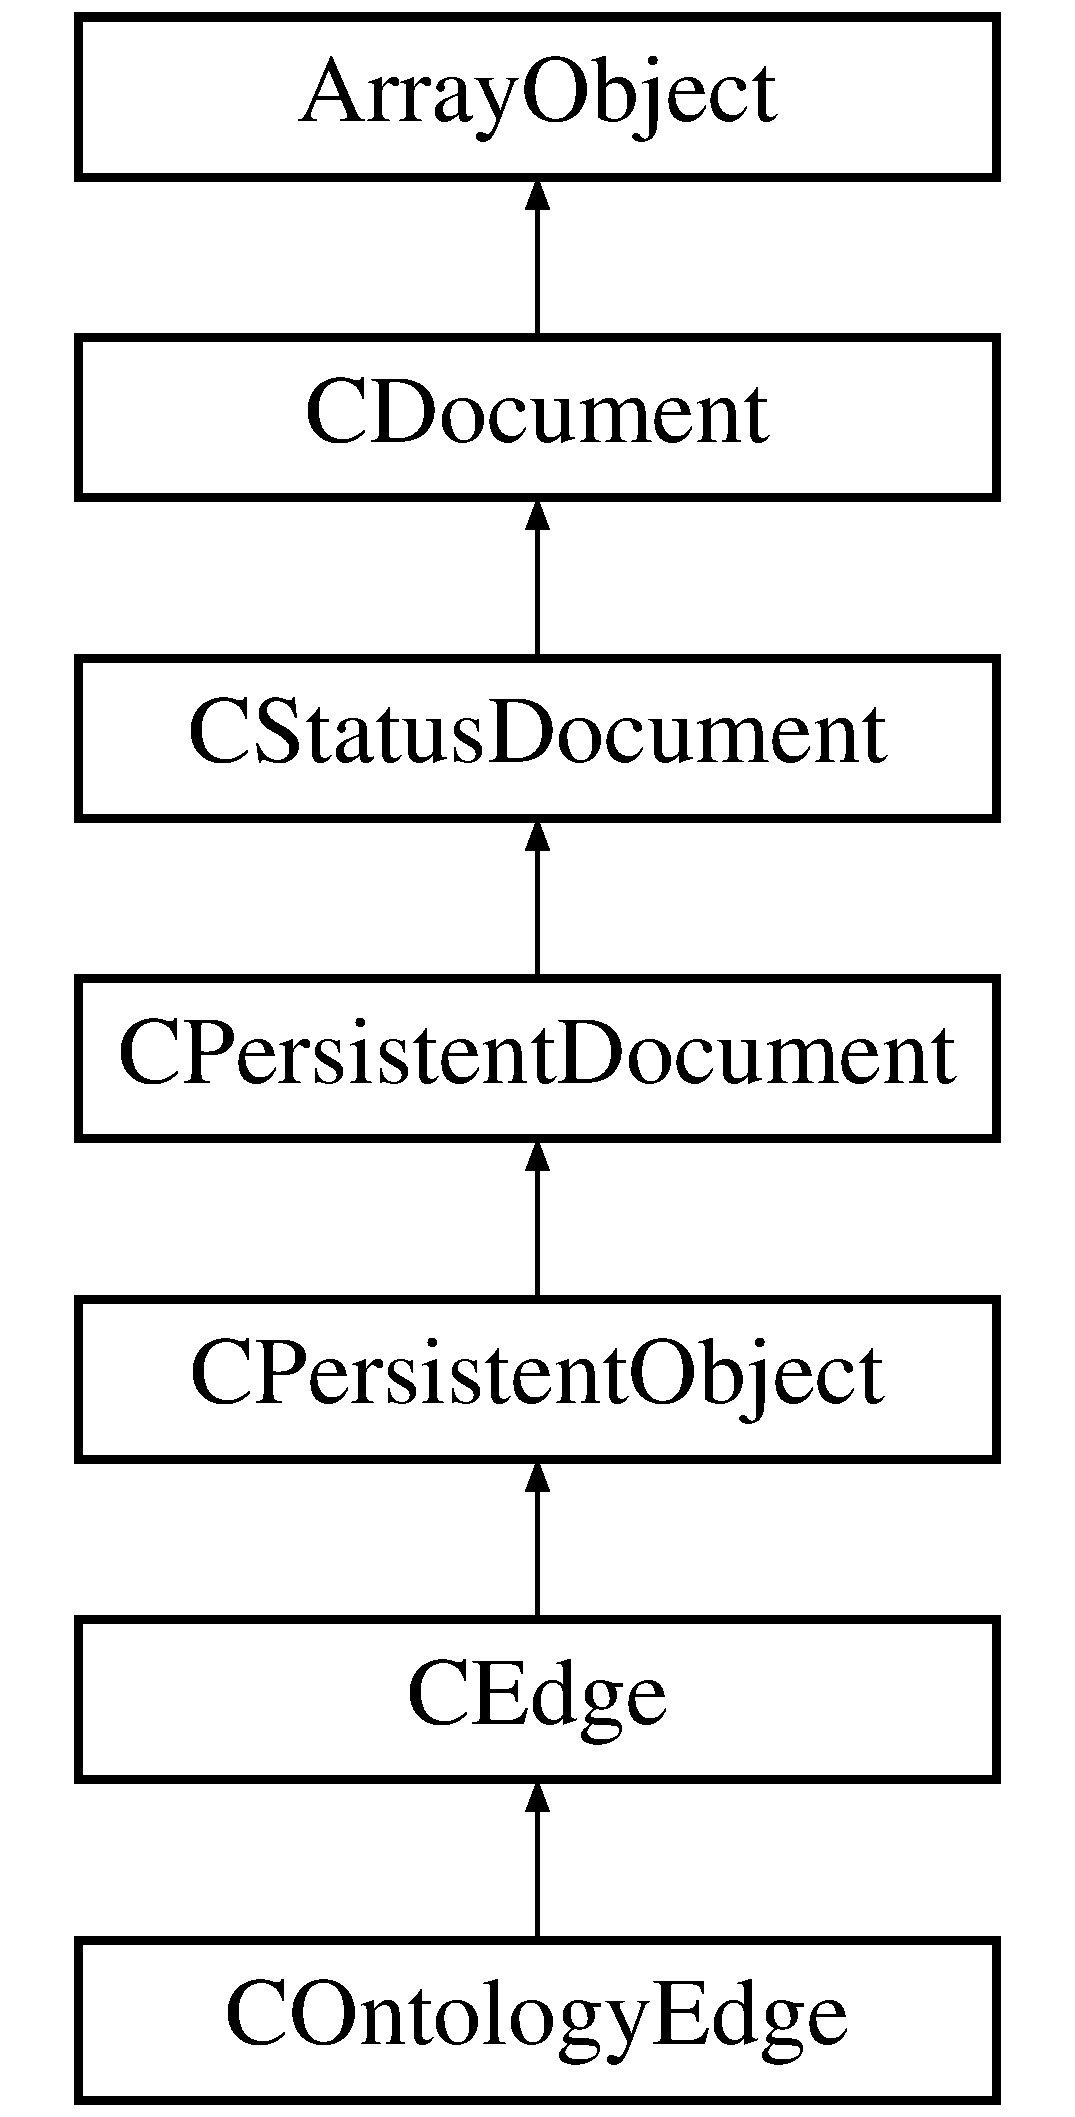
\includegraphics[height=7.000000cm]{class_c_edge}
\end{center}
\end{figure}
\subsection*{Public Member Functions}
\begin{DoxyCompactItemize}
\item 
\hyperlink{class_c_edge_a8031397d41fb274570fbbd68948c1841}{Subject} (\$the\-Value=N\-U\-L\-L, \$get\-Old=F\-A\-L\-S\-E)
\item 
\hyperlink{class_c_edge_ab86f5f67f0577c957ac9f2c0493f0e39}{Predicate} (\$the\-Value=N\-U\-L\-L, \$get\-Old=F\-A\-L\-S\-E)
\item 
\hyperlink{class_c_edge_a16960ecedab5d747b46f9d7ac9ddf9eb}{Object} (\$the\-Value=N\-U\-L\-L, \$get\-Old=F\-A\-L\-S\-E)
\end{DoxyCompactItemize}
\subsection*{Protected Member Functions}
\begin{DoxyCompactItemize}
\item 
\hyperlink{class_c_edge_a2b7580b50c8c50ff2382a229c6435211}{\-\_\-index} (\hyperlink{class_c_connection}{C\-Connection} \$the\-Connection, \$the\-Modifiers)
\item 
\hyperlink{class_c_edge_ac9dd0f883ce7867d0a5482eed84fe7f0}{\-\_\-\-Preunset} (\&\$the\-Offset)
\item 
\hyperlink{class_c_edge_a53e2c3f7c502c586554f70f5749d4c2d}{\-\_\-\-Ready} ()
\end{DoxyCompactItemize}
\subsection*{Additional Inherited Members}


\subsection{Member Function Documentation}
\hypertarget{class_c_edge_a2b7580b50c8c50ff2382a229c6435211}{\index{C\-Edge@{C\-Edge}!\-\_\-index@{\-\_\-index}}
\index{\-\_\-index@{\-\_\-index}!CEdge@{C\-Edge}}
\subsubsection[{\-\_\-index}]{\setlength{\rightskip}{0pt plus 5cm}C\-Edge\-::\-\_\-index (
\begin{DoxyParamCaption}
\item[{{\bf C\-Connection}}]{\$the\-Connection, }
\item[{}]{\$the\-Modifiers}
\end{DoxyParamCaption}
)\hspace{0.3cm}{\ttfamily [protected]}}}\label{class_c_edge_a2b7580b50c8c50ff2382a229c6435211}
\subparagraph*{Return the object's global unique identifier}

The edge class defines the global identifier, \hyperlink{}{k\-T\-A\-G\-\_\-\-G\-I\-D}, as the concatenation of the subject, predicate and object offsets converted to string.

In this method we check whether all three are present, or we raise an exception.


\begin{DoxyParams}[1]{Parameters}
\hyperlink{class_c_connection}{C\-Connection} & {\em \$the\-Connection} & Server, database or container. \\
\hline
bitfield & {\em \$the\-Modifiers} & Commit options.\\
\hline
\end{DoxyParams}

\begin{DoxyExceptions}{Exceptions}
{\em Exception} & protected \\
\hline
\end{DoxyExceptions}
\begin{DoxyReturn}{Returns}
string$|$\-N\-U\-L\-L The object's global unique identifier.
\end{DoxyReturn}
\begin{DoxySeeAlso}{See Also}
k\-T\-A\-G\-\_\-\-S\-U\-B\-J\-E\-C\-T k\-T\-A\-G\-\_\-\-P\-R\-E\-D\-I\-C\-A\-T\-E k\-T\-A\-G\-\_\-\-O\-B\-J\-E\-C\-T 

k\-T\-O\-K\-E\-N\-\_\-\-I\-N\-D\-E\-X\-\_\-\-S\-E\-P\-A\-R\-A\-T\-O\-R 
\end{DoxySeeAlso}
\hypertarget{class_c_edge_ac9dd0f883ce7867d0a5482eed84fe7f0}{\index{C\-Edge@{C\-Edge}!\-\_\-\-Preunset@{\-\_\-\-Preunset}}
\index{\-\_\-\-Preunset@{\-\_\-\-Preunset}!CEdge@{C\-Edge}}
\subsubsection[{\-\_\-\-Preunset}]{\setlength{\rightskip}{0pt plus 5cm}C\-Edge\-::\-\_\-\-Preunset (
\begin{DoxyParamCaption}
\item[{\&}]{\$the\-Offset}
\end{DoxyParamCaption}
)\hspace{0.3cm}{\ttfamily [protected]}}}\label{class_c_edge_ac9dd0f883ce7867d0a5482eed84fe7f0}
\subparagraph*{Handle offset before unsetting it}

In this class we prevent the modification of the \hyperlink{}{k\-T\-A\-G\-\_\-\-S\-U\-B\-J\-E\-C\-T}, \hyperlink{}{k\-T\-A\-G\-\_\-\-P\-R\-E\-D\-I\-C\-A\-T\-E} and \hyperlink{}{k\-T\-A\-G\-\_\-\-O\-B\-J\-E\-C\-T} offsets if the object is committed.


\begin{DoxyParams}[1]{Parameters}
reference & {\em \&\$the\-Offset} & Offset.\\
\hline
\end{DoxyParams}
protected


\begin{DoxyExceptions}{Exceptions}
{\em Exception} & \hyperlink{class_c_status_document_ab7d96fd4588cf7d5432fc65a1d1fb076}{\-\_\-\-Is\-Committed()}\\
\hline
\end{DoxyExceptions}
\begin{DoxySeeAlso}{See Also}
k\-T\-A\-G\-\_\-\-S\-U\-B\-J\-E\-C\-T k\-T\-A\-G\-\_\-\-P\-R\-E\-D\-I\-C\-A\-T\-E k\-T\-A\-G\-\_\-\-O\-B\-J\-E\-C\-T 
\end{DoxySeeAlso}
\hypertarget{class_c_edge_a53e2c3f7c502c586554f70f5749d4c2d}{\index{C\-Edge@{C\-Edge}!\-\_\-\-Ready@{\-\_\-\-Ready}}
\index{\-\_\-\-Ready@{\-\_\-\-Ready}!CEdge@{C\-Edge}}
\subsubsection[{\-\_\-\-Ready}]{\setlength{\rightskip}{0pt plus 5cm}C\-Edge\-::\-\_\-\-Ready (
\begin{DoxyParamCaption}
{}
\end{DoxyParamCaption}
)\hspace{0.3cm}{\ttfamily [protected]}}}\label{class_c_edge_a53e2c3f7c502c586554f70f5749d4c2d}
\subparagraph*{Determine if the object is ready}

In this class we tie the \hyperlink{class_c_status_document_a954dee06e219e0a0f2e7fa6edac56e28}{\-\_\-\-Is\-Inited()} status to the presence or absence of the \hyperlink{}{k\-T\-A\-G\-\_\-\-S\-U\-B\-J\-E\-C\-T}, \hyperlink{}{k\-T\-A\-G\-\_\-\-P\-R\-E\-D\-I\-C\-A\-T\-E} and \hyperlink{}{k\-T\-A\-G\-\_\-\-O\-B\-J\-E\-C\-T} offsets.

protected \begin{DoxyReturn}{Returns}
boolean {\ttfamily T\-R\-U\-E} means \hyperlink{}{.  \-\_\-\-Ready()  k\-T\-A\-G\-\_\-\-S\-U\-B\-J\-E\-C\-T k\-T\-A\-G\-\_\-\-P\-R\-E\-D\-I\-C\-A\-T\-E k\-T\-A\-G\-\_\-\-O\-B\-J\-E\-C\-T }
\end{DoxyReturn}
\hypertarget{class_c_edge_a16960ecedab5d747b46f9d7ac9ddf9eb}{\index{C\-Edge@{C\-Edge}!Object@{Object}}
\index{Object@{Object}!CEdge@{C\-Edge}}
\subsubsection[{Object}]{\setlength{\rightskip}{0pt plus 5cm}C\-Edge\-::\-Object (
\begin{DoxyParamCaption}
\item[{}]{\$the\-Value = {\ttfamily NULL}, }
\item[{}]{\$get\-Old = {\ttfamily FALSE}}
\end{DoxyParamCaption}
)}}\label{class_c_edge_a16960ecedab5d747b46f9d7ac9ddf9eb}
\subparagraph*{Manage edge object}

This method can be used to manage the edge's object vertex, \hyperlink{}{k\-T\-A\-G\-\_\-\-O\-B\-J\-E\-C\-T}, which is a reference to an object that represents the destination of the relationship this edge represents.

The method accepts a parameter which represents the vertex, or the requested operation, depending on its value\-:


\begin{DoxyItemize}
\item {\ttfamily N\-U\-L\-L}\-: Return the current value. 
\item {\ttfamily F\-A\-L\-S\-E}\-: Delete the current value. 
\item {\itshape other}\-: Set the value with the provided parameter. 
\end{DoxyItemize}

The second parameter is a boolean which if {\ttfamily T\-R\-U\-E} will return the {\itshape old} value when replacing containers; if {\ttfamily F\-A\-L\-S\-E}, it will return the currently set value.

Note that when the object has the \hyperlink{class_c_status_document_ab7d96fd4588cf7d5432fc65a1d1fb076}{\-\_\-\-Is\-Committed()} status this offset will be locked and an exception will be raised.


\begin{DoxyParams}[1]{Parameters}
mixed & {\em \$the\-Value} & Vertex or operation. \\
\hline
boolean & {\em \$get\-Old} & {\ttfamily T\-R\-U\-E} get old value.\\
\hline
\end{DoxyParams}
public \begin{DoxyReturn}{Returns}
mixed {\itshape New} or {\itshape old} native container.
\end{DoxyReturn}
Manage\-Offset()

\begin{DoxySeeAlso}{See Also}
k\-T\-A\-G\-\_\-\-O\-B\-J\-E\-C\-T 
\end{DoxySeeAlso}
\hypertarget{class_c_edge_ab86f5f67f0577c957ac9f2c0493f0e39}{\index{C\-Edge@{C\-Edge}!Predicate@{Predicate}}
\index{Predicate@{Predicate}!CEdge@{C\-Edge}}
\subsubsection[{Predicate}]{\setlength{\rightskip}{0pt plus 5cm}C\-Edge\-::\-Predicate (
\begin{DoxyParamCaption}
\item[{}]{\$the\-Value = {\ttfamily NULL}, }
\item[{}]{\$get\-Old = {\ttfamily FALSE}}
\end{DoxyParamCaption}
)}}\label{class_c_edge_ab86f5f67f0577c957ac9f2c0493f0e39}
\subparagraph*{Manage edge predicate}

This method can be used to manage the edge's predicate, \hyperlink{}{k\-T\-A\-G\-\_\-\-P\-R\-E\-D\-I\-C\-A\-T\-E}, which is a reference to an object that represents the origin of the relationship this edge represents.

The method accepts a parameter which represents the predicate, or the requested operation, depending on its value\-:


\begin{DoxyItemize}
\item {\ttfamily N\-U\-L\-L}\-: Return the current value. 
\item {\ttfamily F\-A\-L\-S\-E}\-: Delete the current value. 
\item {\itshape other}\-: Set the value with the provided parameter. 
\end{DoxyItemize}

The second parameter is a boolean which if {\ttfamily T\-R\-U\-E} will return the {\itshape old} value when replacing containers; if {\ttfamily F\-A\-L\-S\-E}, it will return the currently set value.

Note that when the object has the \hyperlink{class_c_status_document_ab7d96fd4588cf7d5432fc65a1d1fb076}{\-\_\-\-Is\-Committed()} status this offset will be locked and an exception will be raised.


\begin{DoxyParams}[1]{Parameters}
mixed & {\em \$the\-Value} & Predicate or operation. \\
\hline
boolean & {\em \$get\-Old} & {\ttfamily T\-R\-U\-E} get old value.\\
\hline
\end{DoxyParams}
public \begin{DoxyReturn}{Returns}
mixed {\itshape New} or {\itshape old} native container.
\end{DoxyReturn}
Manage\-Offset()

\begin{DoxySeeAlso}{See Also}
k\-T\-A\-G\-\_\-\-P\-R\-E\-D\-I\-C\-A\-T\-E 
\end{DoxySeeAlso}
\hypertarget{class_c_edge_a8031397d41fb274570fbbd68948c1841}{\index{C\-Edge@{C\-Edge}!Subject@{Subject}}
\index{Subject@{Subject}!CEdge@{C\-Edge}}
\subsubsection[{Subject}]{\setlength{\rightskip}{0pt plus 5cm}C\-Edge\-::\-Subject (
\begin{DoxyParamCaption}
\item[{}]{\$the\-Value = {\ttfamily NULL}, }
\item[{}]{\$get\-Old = {\ttfamily FALSE}}
\end{DoxyParamCaption}
)}}\label{class_c_edge_a8031397d41fb274570fbbd68948c1841}
\subparagraph*{Manage edge subject}

This method can be used to manage the edge's subject vertex, \hyperlink{}{k\-T\-A\-G\-\_\-\-S\-U\-B\-J\-E\-C\-T}, which is a reference to an object that represents the origin of the relationship this edge represents.

The method accepts a parameter which represents the vertex, or the requested operation, depending on its value\-:


\begin{DoxyItemize}
\item {\ttfamily N\-U\-L\-L}\-: Return the current value. 
\item {\ttfamily F\-A\-L\-S\-E}\-: Delete the current value. 
\item {\itshape other}\-: Set the value with the provided parameter. 
\end{DoxyItemize}

The second parameter is a boolean which if {\ttfamily T\-R\-U\-E} will return the {\itshape old} value when replacing containers; if {\ttfamily F\-A\-L\-S\-E}, it will return the currently set value.

Note that when the object has the \hyperlink{class_c_status_document_ab7d96fd4588cf7d5432fc65a1d1fb076}{\-\_\-\-Is\-Committed()} status this offset will be locked and an exception will be raised.


\begin{DoxyParams}[1]{Parameters}
mixed & {\em \$the\-Value} & Vertex or operation. \\
\hline
boolean & {\em \$get\-Old} & {\ttfamily T\-R\-U\-E} get old value.\\
\hline
\end{DoxyParams}
public \begin{DoxyReturn}{Returns}
mixed {\itshape New} or {\itshape old} native container.
\end{DoxyReturn}
Manage\-Offset()

\begin{DoxySeeAlso}{See Also}
k\-T\-A\-G\-\_\-\-S\-U\-B\-J\-E\-C\-T 
\end{DoxySeeAlso}


The documentation for this class was generated from the following file\-:\begin{DoxyCompactItemize}
\item 
/\-Library/\-Web\-Server/\-Library/\-P\-H\-P\-Wrapper/classes/C\-Edge.\-php\end{DoxyCompactItemize}

\hypertarget{class_c_exception}{\section{C\-Exception Class Reference}
\label{class_c_exception}\index{C\-Exception@{C\-Exception}}
}
Inheritance diagram for C\-Exception\-:\begin{figure}[H]
\begin{center}
\leavevmode
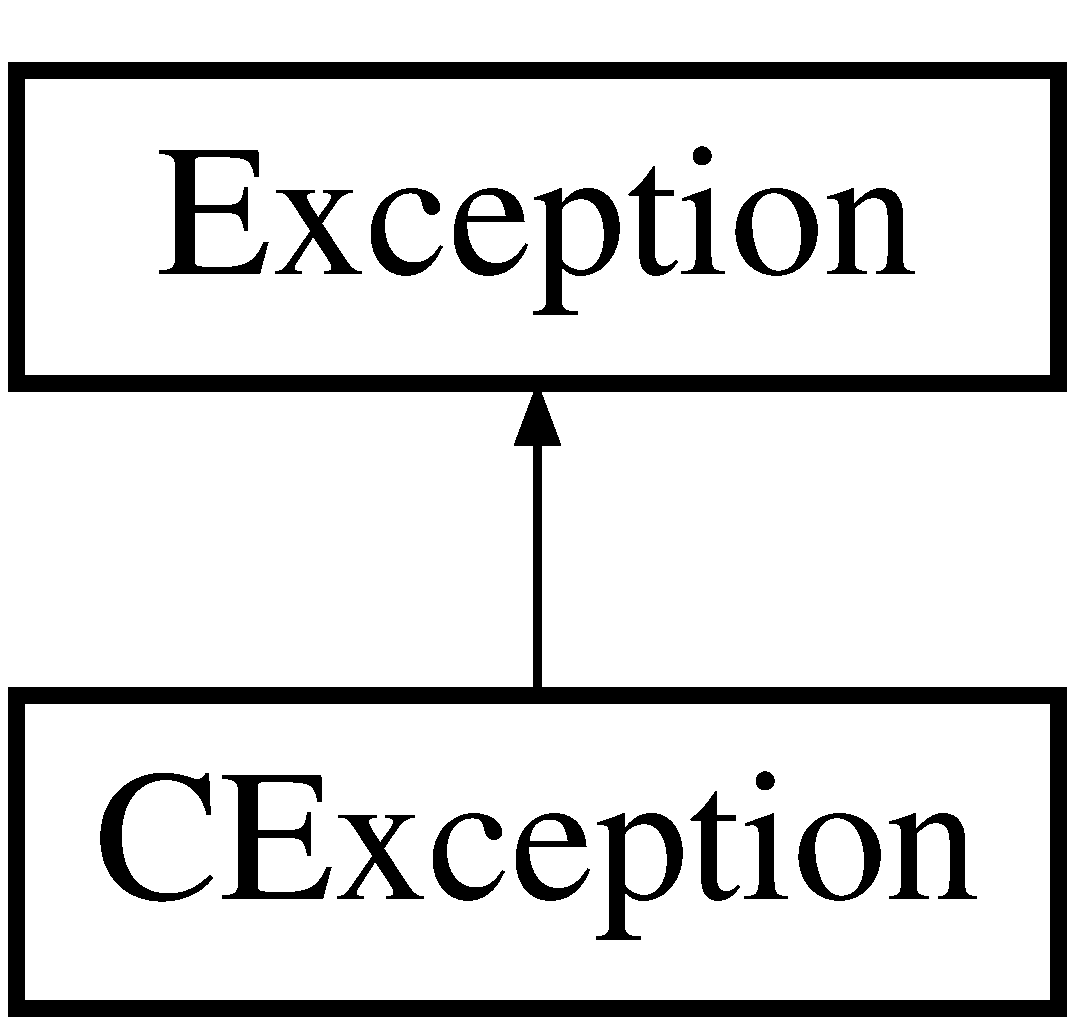
\includegraphics[height=2.000000cm]{class_c_exception}
\end{center}
\end{figure}
\subsection*{Public Member Functions}
\begin{DoxyCompactItemize}
\item 
\hyperlink{class_c_exception_aea9f2ae76b6058652dfb672ce1a78507}{\-\_\-\-\_\-construct} (\$the\-Message=N\-U\-L\-L, \$the\-Code=N\-U\-L\-L, \$the\-Severity=N\-U\-L\-L, \$the\-References=N\-U\-L\-L, \$the\-Previous=N\-U\-L\-L)
\item 
\hyperlink{class_c_exception_a06b1b207799f8a8ca27bc12d1be82b07}{\-\_\-\-\_\-to\-String} ()
\item 
\hyperlink{class_c_exception_a2bef90da8a35e80dda8072d4f748ec20}{Severity} (\$the\-Value=N\-U\-L\-L)
\item 
\hyperlink{class_c_exception_abcbd46a262790fcbe3493e30a6418821}{Reference} (\$the\-Index=N\-U\-L\-L, \$the\-Value=N\-U\-L\-L)
\end{DoxyCompactItemize}
\subsection*{Static Public Member Functions}
\begin{DoxyCompactItemize}
\item 
static \hyperlink{class_c_exception_a99be238dee92094374995eebe54df6a8}{As\-H\-T\-M\-L} (Exception \$the\-Exception)
\item 
static \hyperlink{class_c_exception_ad5f92d9c5d11443ce4b69aec6a8484d5}{\-\_\-\-Trace} (Exception \$the\-Exception)
\item 
static \hyperlink{class_c_exception_a643b0ad0d3d4faba071968c953d639af}{\-\_\-\-Trace2\-H\-T\-M\-L} (D\-O\-M\-Node \$the\-Table, \$the\-Element)
\item 
static \hyperlink{class_c_exception_a84a97fbcc2907c16a29a01adf841ee94}{\-\_\-\-Exception2\-H\-T\-M\-L} (\$the\-Table, \$the\-Element, \$the\-Source=N\-U\-L\-L)
\end{DoxyCompactItemize}
\subsection*{Static Protected Member Functions}
\begin{DoxyCompactItemize}
\item 
static \hyperlink{class_c_exception_a84f7c3fe4e048f28881432a1fc138ffc}{\-\_\-\-Trace\-Argument\-String} (\$the\-Value)
\end{DoxyCompactItemize}
\subsection*{Protected Attributes}
\begin{DoxyCompactItemize}
\item 
\hypertarget{class_c_exception_aa544b648ee9ef87c6bea3571737f10f6}{{\bfseries \$m\-Severity} = N\-U\-L\-L}\label{class_c_exception_aa544b648ee9ef87c6bea3571737f10f6}

\item 
\hypertarget{class_c_exception_a483fdc73c7a4726532dff474c97a4eb7}{{\bfseries \$m\-References} = Array()}\label{class_c_exception_a483fdc73c7a4726532dff474c97a4eb7}

\end{DoxyCompactItemize}


\subsection{Constructor \& Destructor Documentation}
\hypertarget{class_c_exception_aea9f2ae76b6058652dfb672ce1a78507}{\index{C\-Exception@{C\-Exception}!\-\_\-\-\_\-construct@{\-\_\-\-\_\-construct}}
\index{\-\_\-\-\_\-construct@{\-\_\-\-\_\-construct}!CException@{C\-Exception}}
\subsubsection[{\-\_\-\-\_\-construct}]{\setlength{\rightskip}{0pt plus 5cm}C\-Exception\-::\-\_\-\-\_\-construct (
\begin{DoxyParamCaption}
\item[{}]{\$the\-Message = {\ttfamily NULL}, }
\item[{}]{\$the\-Code = {\ttfamily NULL}, }
\item[{}]{\$the\-Severity = {\ttfamily NULL}, }
\item[{}]{\$the\-References = {\ttfamily NULL}, }
\item[{}]{\$the\-Previous = {\ttfamily NULL}}
\end{DoxyParamCaption}
)}}\label{class_c_exception_aea9f2ae76b6058652dfb672ce1a78507}
Instantiate class.

The first two parameters follow the inherited interface, the constructor adds support for the extended class members\-:


\begin{DoxyItemize}
\item {\bfseries \$the\-Message}\-: This parameter represents the inherited {\itshape message}. 
\item {\bfseries \$the\-Code}\-: This parameter represents the inherited {\itshape code}. 
\item {\bfseries \$the\-Severity}\-: This parameter holds \hyperlink{class_c_exception_a2bef90da8a35e80dda8072d4f748ec20}{the} exception type, level or severity\-: 
\begin{DoxyItemize}
\item {\itshape \hyperlink{}{k\-S\-T\-A\-T\-U\-S\-\_\-\-I\-D\-L\-E}}\-: This indicates an idle state. 
\item {\itshape \hyperlink{}{k\-S\-T\-A\-T\-U\-S\-\_\-\-N\-O\-T\-I\-C\-E}}\-: This indicates an informative note or message. 
\item {\itshape \hyperlink{}{k\-S\-T\-A\-T\-U\-S\-\_\-\-W\-A\-R\-N\-I\-N\-G}}\-: This indicates a warning. 
\item {\itshape \hyperlink{}{k\-S\-T\-A\-T\-U\-S\-\_\-\-E\-R\-R\-O\-R}}\-: This indicates an error. 
\item {\itshape \hyperlink{}{k\-S\-T\-A\-T\-U\-S\-\_\-\-F\-A\-T\-A\-L}}\-: This indicates a fatal error, in general this should halt program execution. 
\item {\itshape \hyperlink{}{k\-S\-T\-A\-T\-U\-S\-\_\-\-B\-U\-G}}\-: This indicates a bug, such exceptions should be logged and forwarded to developers. 
\end{DoxyItemize}
\item {\bfseries \$the\-References}\-: This parameter holds the exception's references \hyperlink{}{list}, it is an array indexed by reference label or term holding the reference value as value. 
\item {\bfseries \$the\-Previous}\-: This parameter represents the previous exception when forwarding. 
\end{DoxyItemize}


\begin{DoxyParams}[1]{Parameters}
string & {\em \$the\-Message} & Exception message. \\
\hline
integer & {\em \$the\-Code} & Exception code. \\
\hline
string & {\em \$the\-Severity} & Exception severity. \\
\hline
array & {\em \$the\-References} & Exception references. \\
\hline
Exception & {\em \$the\-Previous} & Previous exception.\\
\hline
\end{DoxyParams}
public

Code\-User()  User\-Messages()  User\-Namespace()  \hyperlink{class_c_exception_a2bef90da8a35e80dda8072d4f748ec20}{Severity()}  \hyperlink{class_c_exception_abcbd46a262790fcbe3493e30a6418821}{Reference()} 

\subsection{Member Function Documentation}
\hypertarget{class_c_exception_a06b1b207799f8a8ca27bc12d1be82b07}{\index{C\-Exception@{C\-Exception}!\-\_\-\-\_\-to\-String@{\-\_\-\-\_\-to\-String}}
\index{\-\_\-\-\_\-to\-String@{\-\_\-\-\_\-to\-String}!CException@{C\-Exception}}
\subsubsection[{\-\_\-\-\_\-to\-String}]{\setlength{\rightskip}{0pt plus 5cm}C\-Exception\-::\-\_\-\-\_\-to\-String (
\begin{DoxyParamCaption}
{}
\end{DoxyParamCaption}
)}}\label{class_c_exception_a06b1b207799f8a8ca27bc12d1be82b07}
Return the object name.

In this class we return the stack trace.

public \begin{DoxyReturn}{Returns}
string The stack trace. 
\end{DoxyReturn}
\hypertarget{class_c_exception_a84a97fbcc2907c16a29a01adf841ee94}{\index{C\-Exception@{C\-Exception}!\-\_\-\-Exception2\-H\-T\-M\-L@{\-\_\-\-Exception2\-H\-T\-M\-L}}
\index{\-\_\-\-Exception2\-H\-T\-M\-L@{\-\_\-\-Exception2\-H\-T\-M\-L}!CException@{C\-Exception}}
\subsubsection[{\-\_\-\-Exception2\-H\-T\-M\-L}]{\setlength{\rightskip}{0pt plus 5cm}static C\-Exception\-::\-\_\-\-Exception2\-H\-T\-M\-L (
\begin{DoxyParamCaption}
\item[{}]{\$the\-Table, }
\item[{}]{\$the\-Element, }
\item[{}]{\$the\-Source = {\ttfamily NULL}}
\end{DoxyParamCaption}
)\hspace{0.3cm}{\ttfamily [static]}}}\label{class_c_exception_a84a97fbcc2907c16a29a01adf841ee94}
Return the exception as H\-T\-M\-L.

This method can be used to return the provided exception as H\-T\-M\-L code, it is assumed that the element will be placed in an H\-T\-M\-L table, so the method will return a series of table rows.

The method accepts the following parameters\-:


\begin{DoxyItemize}
\item {\bfseries \$the\-Table}\-: The H\-T\-M\-L table in which we want to place the trace. 
\item {\bfseries \$the\-Element}\-: The exception, it must be an Exception, if any other type is passed, the method will return {\itshape N\-U\-L\-L}. 
\item {\bfseries \$the\-Source}\-: This parameter is used to provide a link to the source file\-: 
\begin{DoxyItemize}
\item {\itshape N\-U\-L\-L}\-: No source file management. 
\item {\itshape T\-R\-U\-E}\-: The default source file viewer will be used. 
\item {\itshape string}\-: The method will execute the provided string as a shell command line. 
\end{DoxyItemize}
\end{DoxyItemize}


\begin{DoxyParams}[1]{Parameters}
D\-O\-M\-Element & {\em \$the\-Table} & H\-T\-M\-L table. \\
\hline
array & {\em \$the\-Element} & Trace element. \\
\hline
N\-U\-L\-L | T\-R\-U\-E | string & {\em \$the\-Source} & Source file control. \\
\hline
\end{DoxyParams}
\hypertarget{class_c_exception_ad5f92d9c5d11443ce4b69aec6a8484d5}{\index{C\-Exception@{C\-Exception}!\-\_\-\-Trace@{\-\_\-\-Trace}}
\index{\-\_\-\-Trace@{\-\_\-\-Trace}!CException@{C\-Exception}}
\subsubsection[{\-\_\-\-Trace}]{\setlength{\rightskip}{0pt plus 5cm}static C\-Exception\-::\-\_\-\-Trace (
\begin{DoxyParamCaption}
\item[{Exception}]{\$the\-Exception}
\end{DoxyParamCaption}
)\hspace{0.3cm}{\ttfamily [static]}}}\label{class_c_exception_ad5f92d9c5d11443ce4b69aec6a8484d5}
Return the exception trace.

This method can be used to return the exception trace in the order in which it was called. The main utility of this method is to manage forwarded exceptions.

The method will return an array indexed by file path and line number hash in which the value is either an exception or a trace array. If you run in P\-H\-P version $<$ 3.\-0.\-x the first element will be an exception and the others will be traces, if you run a higher version of P\-H\-P you can forward exceptions, so the elements will be mixed.


\begin{DoxyParams}[1]{Parameters}
Exception & {\em \$the\-Exception} & Exception to trace.\\
\hline
\end{DoxyParams}
\begin{DoxyReturn}{Returns}
array 
\end{DoxyReturn}
\hypertarget{class_c_exception_a643b0ad0d3d4faba071968c953d639af}{\index{C\-Exception@{C\-Exception}!\-\_\-\-Trace2\-H\-T\-M\-L@{\-\_\-\-Trace2\-H\-T\-M\-L}}
\index{\-\_\-\-Trace2\-H\-T\-M\-L@{\-\_\-\-Trace2\-H\-T\-M\-L}!CException@{C\-Exception}}
\subsubsection[{\-\_\-\-Trace2\-H\-T\-M\-L}]{\setlength{\rightskip}{0pt plus 5cm}static C\-Exception\-::\-\_\-\-Trace2\-H\-T\-M\-L (
\begin{DoxyParamCaption}
\item[{D\-O\-M\-Node}]{\$the\-Table, }
\item[{}]{\$the\-Element}
\end{DoxyParamCaption}
)\hspace{0.3cm}{\ttfamily [static]}}}\label{class_c_exception_a643b0ad0d3d4faba071968c953d639af}
Return the exception trace element as H\-T\-M\-L.

This method can be used to return the trace element as H\-T\-M\-L code.

The method accepts the following parameters\-:


\begin{DoxyItemize}
\item {\bfseries \$the\-Table}\-: The H\-T\-M\-L table in which we want to place the trace. 
\item {\bfseries \$the\-Element}\-: The trace element, it must be an array, if any other type is passed, the method will return {\itshape N\-U\-L\-L}. 
\end{DoxyItemize}


\begin{DoxyParams}[1]{Parameters}
D\-O\-M\-Node & {\em \$the\-Table} & H\-T\-M\-L table. \\
\hline
array & {\em \$the\-Element} & Trace element. \\
\hline
\end{DoxyParams}
\hypertarget{class_c_exception_a84f7c3fe4e048f28881432a1fc138ffc}{\index{C\-Exception@{C\-Exception}!\-\_\-\-Trace\-Argument\-String@{\-\_\-\-Trace\-Argument\-String}}
\index{\-\_\-\-Trace\-Argument\-String@{\-\_\-\-Trace\-Argument\-String}!CException@{C\-Exception}}
\subsubsection[{\-\_\-\-Trace\-Argument\-String}]{\setlength{\rightskip}{0pt plus 5cm}static C\-Exception\-::\-\_\-\-Trace\-Argument\-String (
\begin{DoxyParamCaption}
\item[{}]{\$the\-Value}
\end{DoxyParamCaption}
)\hspace{0.3cm}{\ttfamily [static]}, {\ttfamily [protected]}}}\label{class_c_exception_a84f7c3fe4e048f28881432a1fc138ffc}
Return the trace argument string.

This method can be used to return the string representation of a trace argument.


\begin{DoxyParams}[1]{Parameters}
mixed & {\em \$the\-Value} & Trace argument.\\
\hline
\end{DoxyParams}
\begin{DoxyReturn}{Returns}
string 
\end{DoxyReturn}
\hypertarget{class_c_exception_a99be238dee92094374995eebe54df6a8}{\index{C\-Exception@{C\-Exception}!As\-H\-T\-M\-L@{As\-H\-T\-M\-L}}
\index{As\-H\-T\-M\-L@{As\-H\-T\-M\-L}!CException@{C\-Exception}}
\subsubsection[{As\-H\-T\-M\-L}]{\setlength{\rightskip}{0pt plus 5cm}static C\-Exception\-::\-As\-H\-T\-M\-L (
\begin{DoxyParamCaption}
\item[{Exception}]{\$the\-Exception}
\end{DoxyParamCaption}
)\hspace{0.3cm}{\ttfamily [static]}}}\label{class_c_exception_a99be238dee92094374995eebe54df6a8}
Display an exception.

This method can be used to display exceptions in a web browser page.


\begin{DoxyParams}[1]{Parameters}
Exception | \hyperlink{class_c_exception}{C\-Exception} & {\em \$the\-Exception} & Exception object.\\
\hline
\end{DoxyParams}
\begin{DoxyReturn}{Returns}
string
\end{DoxyReturn}
\hyperlink{class_c_exception_abcbd46a262790fcbe3493e30a6418821}{Reference()}  Argument()  Value() \hypertarget{class_c_exception_abcbd46a262790fcbe3493e30a6418821}{\index{C\-Exception@{C\-Exception}!Reference@{Reference}}
\index{Reference@{Reference}!CException@{C\-Exception}}
\subsubsection[{Reference}]{\setlength{\rightskip}{0pt plus 5cm}C\-Exception\-::\-Reference (
\begin{DoxyParamCaption}
\item[{}]{\$the\-Index = {\ttfamily NULL}, }
\item[{}]{\$the\-Value = {\ttfamily NULL}}
\end{DoxyParamCaption}
)}}\label{class_c_exception_abcbd46a262790fcbe3493e30a6418821}
Set or return an exception reference.

This method can be used to set, retrieve and remove exception references. References are a key/value pair that provide additional information on the exception.


\begin{DoxyItemize}
\item {\bfseries \$the\-Index}\-: This represents the reference label or name, if you provide the parameter, it will be used as an array index to either retrieve, set or remove elements, depending on the next parameter's value. If you omit the parameter or pass {\itshape N\-U\-L\-L} the method will consider the whole list of references. 
\item {\bfseries \$the\-Value}\-: This represents the reference value\-: 
\begin{DoxyItemize}
\item {\itshape N\-U\-L\-L}\-: This value indicates that we want to retrieve a reference. If {\itshape \$the\-Index} is provided, the method will return the entry matching it, if there is no match, the method will return {\itshape N\-U\-L\-L}. If {\itshape \$the\-Index} is omitted or {\itshape N\-U\-L\-L}, the method will return the full references array. 
\item {\itshape F\-A\-L\-S\-E}\-: This value indicates that we want to delete a reference. If {\itshape \$the\-Index} is provided, the method will delete the entry matching it and return {\itshape N\-U\-L\-L}. If {\itshape \$the\-Index} is omitted or {\itshape N\-U\-L\-L}, the method will delete all references and return an empty array. 
\item {\itshape Any other type}\-: Other types of value are considered as a value to replace or be added to the references list\-: if {\itshape \$the\-Index} is provided, the method will add or replace the matching element in the list and return the eventual value {\itshape after} it was modified. If {\itshape \$the\-Index} is omitted or {\itshape N\-U\-L\-L}, the operation depends on the type of value\-: 
\begin{DoxyItemize}
\item {\itshape array}\-: The provided array will replace the current list and the method will return the list {\itshape after} it was replaced. 
\item {\itshape Any other type}\-: The provided value will be appended to the list by using a numeric index and the method will always return the provided value. 
\end{DoxyItemize}
\end{DoxyItemize}
\end{DoxyItemize}


\begin{DoxyParams}[1]{Parameters}
mixed & {\em \$the\-Index} & Reference element index. \\
\hline
mixed & {\em \$the\-Value} & N\-U\-L\-L, F\-A\-L\-S\-E, reference value or list.\\
\hline
\end{DoxyParams}
public \begin{DoxyReturn}{Returns}
mixed Exception reference. 
\end{DoxyReturn}
\hypertarget{class_c_exception_a2bef90da8a35e80dda8072d4f748ec20}{\index{C\-Exception@{C\-Exception}!Severity@{Severity}}
\index{Severity@{Severity}!CException@{C\-Exception}}
\subsubsection[{Severity}]{\setlength{\rightskip}{0pt plus 5cm}C\-Exception\-::\-Severity (
\begin{DoxyParamCaption}
\item[{}]{\$the\-Value = {\ttfamily NULL}}
\end{DoxyParamCaption}
)}}\label{class_c_exception_a2bef90da8a35e80dda8072d4f748ec20}
Set or return the exception severity.

When providing {\itshape \$the\-Value}\-:


\begin{DoxyItemize}
\item {\itshape N\-U\-L\-L}\-: Retrieve the current value. 
\item {\itshape F\-A\-L\-S\-E}\-: Reset the value to {\itshape N\-U\-L\-L}. 
\item {\itshape Integer}\-: Set the member to the provided value\-: 
\begin{DoxyItemize}
\item {\itshape \hyperlink{}{k\-S\-T\-A\-T\-U\-S\-\_\-\-I\-D\-L\-E}}\-: Idle state. 
\item {\itshape \hyperlink{}{k\-S\-T\-A\-T\-U\-S\-\_\-\-N\-O\-T\-I\-C\-E}}\-: A notice is an informative message that does not imply an error, nor a situation that should be handled; it can be considered as statistical data. 
\item {\itshape \hyperlink{}{k\-S\-T\-A\-T\-U\-S\-\_\-\-M\-E\-S\-S\-A\-G\-E}}\-: A message is an informative message that is addressed to somebody, although it does not imply an error or warning, it was issued to a receiving party. 
\item {\itshape \hyperlink{}{k\-S\-T\-A\-T\-U\-S\-\_\-\-W\-A\-R\-N\-I\-N\-G}}\-: Warnings are informative data that indicate a potential problem, although they do not imply an error, they indicate a potential problem or an issue that should be addressed at least at a later stage. 
\item {\itshape \hyperlink{}{k\-S\-T\-A\-T\-U\-S\-\_\-\-E\-R\-R\-O\-R}}\-: Errors indicate that something prevented an operation from being performed, this does not necessarily mean that the whole process is halted, but that the results of an operation will not be as expected. 
\item {\itshape \hyperlink{}{k\-S\-T\-A\-T\-U\-S\-\_\-\-F\-A\-T\-A\-L}}\-: Fatal errors are \hyperlink{}{errors} that result in stopping the whole process\-: in this case the error will prevent other operations from being performed and the whole process should be halted. 
\item {\itshape \hyperlink{}{k\-S\-T\-A\-T\-U\-S\-\_\-\-B\-U\-G}}\-: Bugs, as opposed to \hyperlink{}{errors}, result from internal causes independant from external factors. A bug indicates that an operation will never execute as stated, it does not necessarily mean that it is \hyperlink{}{fatal}, but rather that the behaviour of an operation does not correspond to its declaration. 
\end{DoxyItemize}
\end{DoxyItemize}

The above mentioned codes are integer based, each state is represented by an interval, we encourage using the above mentioned codes, but this is not enforced.

When setting or resetting the value, the method will return it {\itshape after} any modification was made.


\begin{DoxyParams}[1]{Parameters}
N\-U\-L\-L | F\-A\-L\-S\-E | integer & {\em \$the\-Value} & N\-U\-L\-L, F\-A\-L\-S\-E or exception severity.\\
\hline
\end{DoxyParams}
public \begin{DoxyReturn}{Returns}
mixed Exception severity or type. 
\end{DoxyReturn}


The documentation for this class was generated from the following file\-:\begin{DoxyCompactItemize}
\item 
/\-Library/\-Web\-Server/\-Library/\-P\-H\-P\-Wrapper/classes/C\-Exception.\-php\end{DoxyCompactItemize}

\hypertarget{class_c_graph_container}{\section{C\-Graph\-Container Class Reference}
\label{class_c_graph_container}\index{C\-Graph\-Container@{C\-Graph\-Container}}
}
Inheritance diagram for C\-Graph\-Container\-:\begin{figure}[H]
\begin{center}
\leavevmode
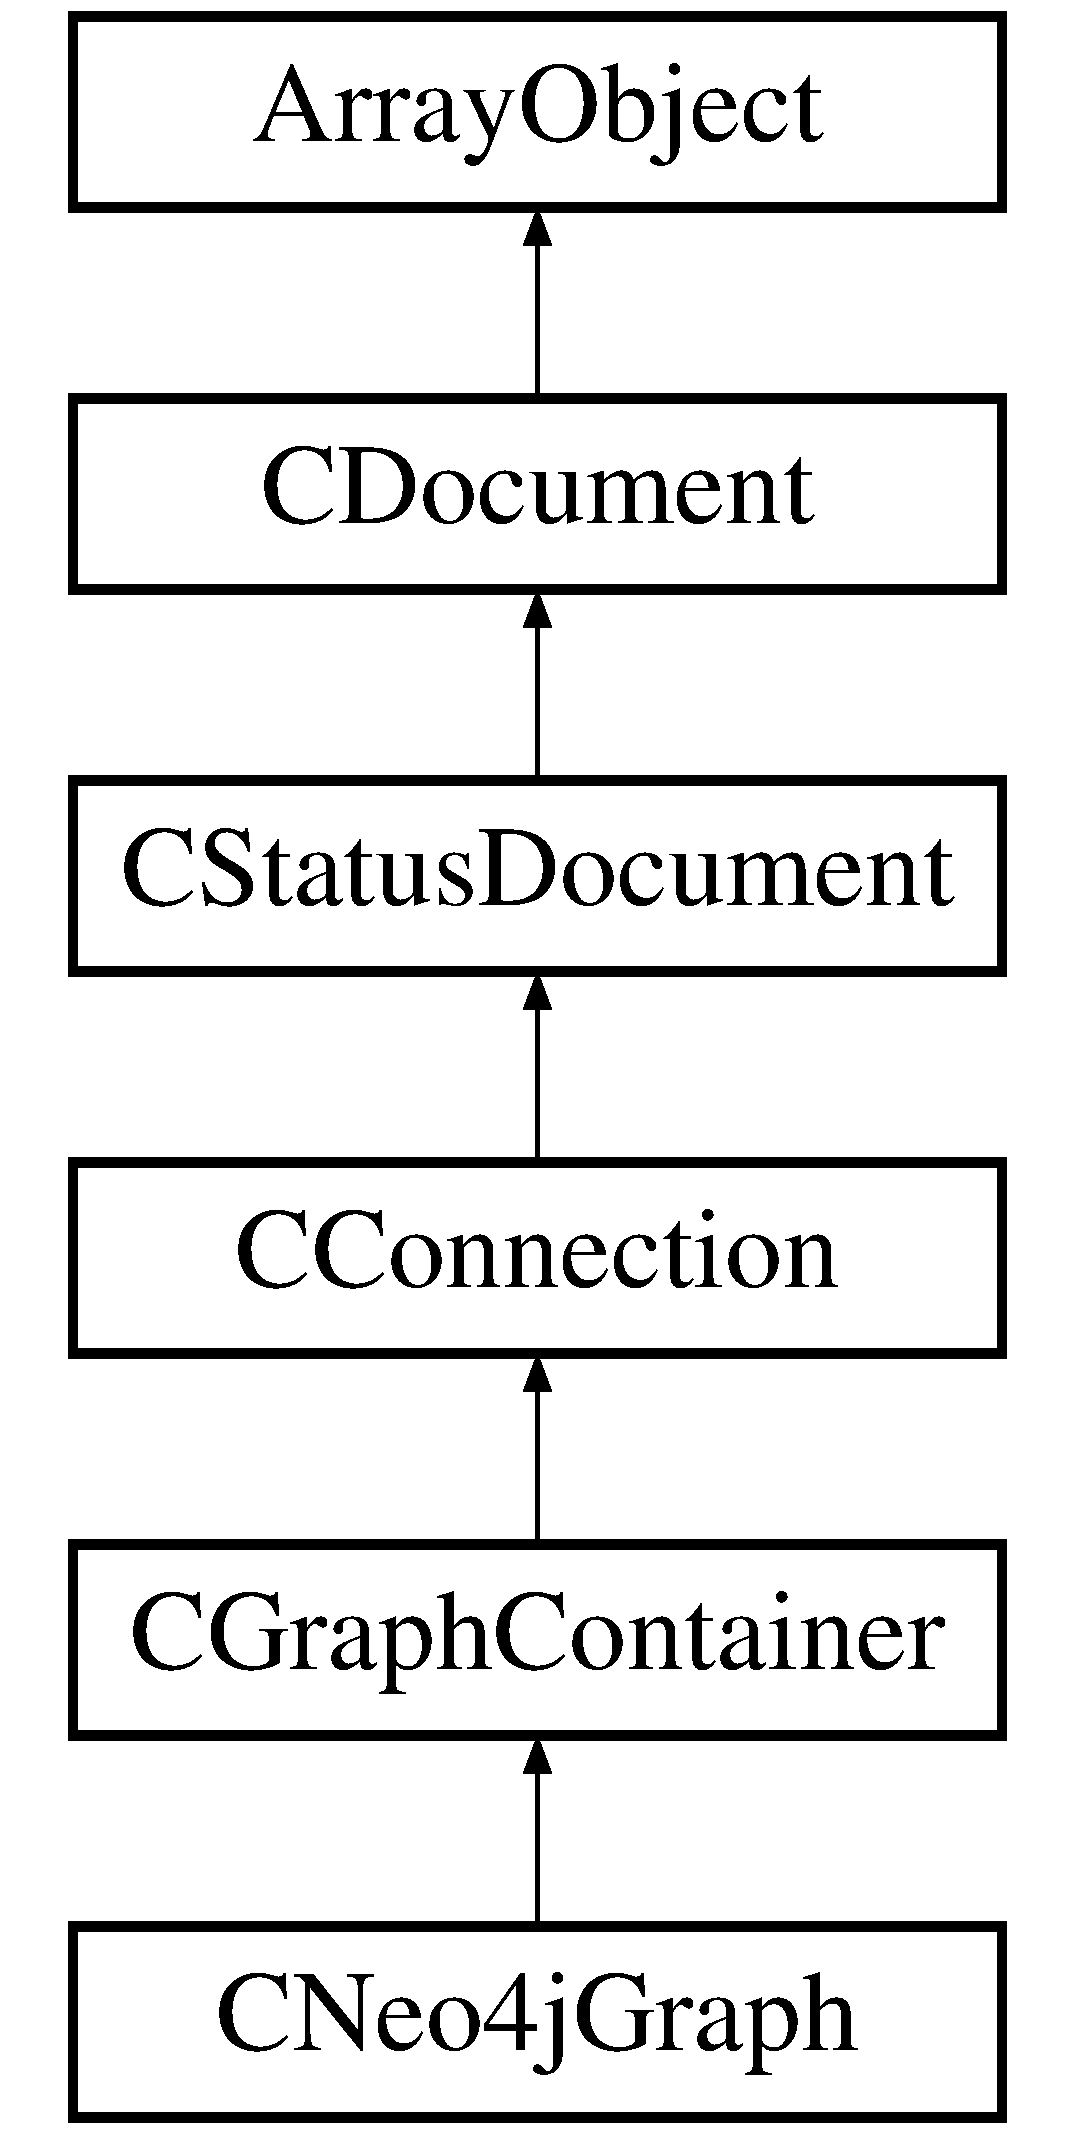
\includegraphics[height=6.000000cm]{class_c_graph_container}
\end{center}
\end{figure}
\subsection*{Public Member Functions}
\begin{DoxyCompactItemize}
\item 
\hyperlink{class_c_graph_container_a59ff4c421da0b86a984c1cf7f81ed50c}{New\-Node} (\$the\-Properties=N\-U\-L\-L)
\item 
\hyperlink{class_c_graph_container_a6bcbff95d7d44d5d59cb479ad0b94db9}{Set\-Node} (\$the\-Node, \$the\-Properties=N\-U\-L\-L)
\item 
\hyperlink{class_c_graph_container_a5ec59fc306eb927f4c1c7c1368d4bc2c}{Get\-Node} (\$the\-Identifier, \$do\-Throw=F\-A\-L\-S\-E)
\item 
\hyperlink{class_c_graph_container_a782de8f208c307af33786f8dc99f9593}{Del\-Node} (\$the\-Identifier)
\item 
\hyperlink{class_c_graph_container_a066acd7a5b35dffeca98610a75866aa4}{New\-Edge} (\$the\-Subject, \$the\-Predicate, \$the\-Object, \$the\-Properties=N\-U\-L\-L)
\item 
\hyperlink{class_c_graph_container_a536acefb01286cc1ccbc211f39179183}{Set\-Edge} (\$the\-Edge)
\item 
\hyperlink{class_c_graph_container_a78ad525680cd1c32e3c52cac29a8fe6a}{Get\-Edge} (\$the\-Identifier)
\item 
\hyperlink{class_c_graph_container_a54ce16d08b2709625069628171d2a6a5}{Del\-Edge} (\$the\-Identifier)
\item 
\hyperlink{class_c_graph_container_a040c1f90e349d61bb8b215ff55afe467}{Get\-Node\-Properties} (\$the\-Node)
\item 
\hyperlink{class_c_graph_container_a1980fc8e492c8f436eb9282f72dc2226}{Get\-Node\-Edges} (\$the\-Node, \$the\-Predicate=N\-U\-L\-L, \$the\-Sense=N\-U\-L\-L)
\end{DoxyCompactItemize}
\subsection*{Additional Inherited Members}


\subsection{Member Function Documentation}
\hypertarget{class_c_graph_container_a54ce16d08b2709625069628171d2a6a5}{\index{C\-Graph\-Container@{C\-Graph\-Container}!Del\-Edge@{Del\-Edge}}
\index{Del\-Edge@{Del\-Edge}!CGraphContainer@{C\-Graph\-Container}}
\subsubsection[{Del\-Edge}]{\setlength{\rightskip}{0pt plus 5cm}C\-Graph\-Container\-::\-Del\-Edge (
\begin{DoxyParamCaption}
\item[{}]{\$the\-Identifier}
\end{DoxyParamCaption}
)\hspace{0.3cm}{\ttfamily [abstract]}}}\label{class_c_graph_container_a54ce16d08b2709625069628171d2a6a5}
\subparagraph*{Delete an existing edge}

This method should delete the provided edge from the current graph.

The method should return {\ttfamily T\-R\-U\-E} if the operation was successful and {\ttfamily N\-U\-L\-L} if the provided identifier is not resolved.


\begin{DoxyParams}[1]{Parameters}
mixed & {\em \$the\-Identifier} & Edge identifier.\\
\hline
\end{DoxyParams}
public \begin{DoxyReturn}{Returns}
mixed 
\end{DoxyReturn}
\hypertarget{class_c_graph_container_a782de8f208c307af33786f8dc99f9593}{\index{C\-Graph\-Container@{C\-Graph\-Container}!Del\-Node@{Del\-Node}}
\index{Del\-Node@{Del\-Node}!CGraphContainer@{C\-Graph\-Container}}
\subsubsection[{Del\-Node}]{\setlength{\rightskip}{0pt plus 5cm}C\-Graph\-Container\-::\-Del\-Node (
\begin{DoxyParamCaption}
\item[{}]{\$the\-Identifier}
\end{DoxyParamCaption}
)\hspace{0.3cm}{\ttfamily [abstract]}}}\label{class_c_graph_container_a782de8f208c307af33786f8dc99f9593}
\subparagraph*{Delete an existing node}

This method should delete the provided node from the current graph.

The method should return {\ttfamily T\-R\-U\-E} if the operation was successful and {\ttfamily N\-U\-L\-L} if the provided identifier is not resolved.


\begin{DoxyParams}[1]{Parameters}
mixed & {\em \$the\-Identifier} & Node identifier.\\
\hline
\end{DoxyParams}
public \begin{DoxyReturn}{Returns}
mixed 
\end{DoxyReturn}
\hypertarget{class_c_graph_container_a78ad525680cd1c32e3c52cac29a8fe6a}{\index{C\-Graph\-Container@{C\-Graph\-Container}!Get\-Edge@{Get\-Edge}}
\index{Get\-Edge@{Get\-Edge}!CGraphContainer@{C\-Graph\-Container}}
\subsubsection[{Get\-Edge}]{\setlength{\rightskip}{0pt plus 5cm}C\-Graph\-Container\-::\-Get\-Edge (
\begin{DoxyParamCaption}
\item[{}]{\$the\-Identifier}
\end{DoxyParamCaption}
)\hspace{0.3cm}{\ttfamily [abstract]}}}\label{class_c_graph_container_a78ad525680cd1c32e3c52cac29a8fe6a}
\subparagraph*{Get an existing edge}

This method should return an edge corresponding to the provided identifier.


\begin{DoxyParams}[1]{Parameters}
mixed & {\em \$the\-Identifier} & Edge identifier.\\
\hline
\end{DoxyParams}
public \begin{DoxyReturn}{Returns}
mixed 
\end{DoxyReturn}
\hypertarget{class_c_graph_container_a5ec59fc306eb927f4c1c7c1368d4bc2c}{\index{C\-Graph\-Container@{C\-Graph\-Container}!Get\-Node@{Get\-Node}}
\index{Get\-Node@{Get\-Node}!CGraphContainer@{C\-Graph\-Container}}
\subsubsection[{Get\-Node}]{\setlength{\rightskip}{0pt plus 5cm}C\-Graph\-Container\-::\-Get\-Node (
\begin{DoxyParamCaption}
\item[{}]{\$the\-Identifier, }
\item[{}]{\$do\-Throw = {\ttfamily FALSE}}
\end{DoxyParamCaption}
)\hspace{0.3cm}{\ttfamily [abstract]}}}\label{class_c_graph_container_a5ec59fc306eb927f4c1c7c1368d4bc2c}
\subparagraph*{Get an existing node}

This method should return a node corresponding to the provided identifier.

If the second parameter is {\ttfamily T\-R\-U\-E} and the node was not found, the method should raise an exception.


\begin{DoxyParams}[1]{Parameters}
mixed & {\em \$the\-Identifier} & Node identifier. \\
\hline
boolean & {\em \$do\-Throw} & T\-R\-U\-E throw exception if not found.\\
\hline
\end{DoxyParams}
public \begin{DoxyReturn}{Returns}
mixed 
\end{DoxyReturn}
\hypertarget{class_c_graph_container_a1980fc8e492c8f436eb9282f72dc2226}{\index{C\-Graph\-Container@{C\-Graph\-Container}!Get\-Node\-Edges@{Get\-Node\-Edges}}
\index{Get\-Node\-Edges@{Get\-Node\-Edges}!CGraphContainer@{C\-Graph\-Container}}
\subsubsection[{Get\-Node\-Edges}]{\setlength{\rightskip}{0pt plus 5cm}C\-Graph\-Container\-::\-Get\-Node\-Edges (
\begin{DoxyParamCaption}
\item[{}]{\$the\-Node, }
\item[{}]{\$the\-Predicate = {\ttfamily NULL}, }
\item[{}]{\$the\-Sense = {\ttfamily NULL}}
\end{DoxyParamCaption}
)\hspace{0.3cm}{\ttfamily [abstract]}}}\label{class_c_graph_container_a1980fc8e492c8f436eb9282f72dc2226}
\subparagraph*{Get node edges}

This method can be used to retrieve the provided node's edges according to the provided sense.

The method accepts the following parameters\-:


\begin{DoxyItemize}
\item {\ttfamily \$the\-Node}\-: The node of which we want the relationships. 
\item {\ttfamily \$the\-Predicate}\-: The eventual predicate or predicates references that must be present in the relationships. 
\item {\ttfamily \$the\-Sense}\-: The relationship direction\-: 
\begin{DoxyItemize}
\item {\ttfamily \hyperlink{}{k\-T\-Y\-P\-E\-\_\-\-R\-E\-L\-A\-T\-I\-O\-N\-\_\-\-I\-N}}\-: Incoming relationships, or all edges that point to the provided node. 
\item {\ttfamily \hyperlink{}{k\-T\-Y\-P\-E\-\_\-\-R\-E\-L\-A\-T\-I\-O\-N\-\_\-\-O\-U\-T}}\-: Outgoing relationships, or all edges to which the current node points to. 
\item {\ttfamily \hyperlink{}{k\-T\-Y\-P\-E\-\_\-\-R\-E\-L\-A\-T\-I\-O\-N\-\_\-\-A\-L\-L}}\-: All relationships, or all edges that point or to which the provided node points to. 
\end{DoxyItemize}
\end{DoxyItemize}

The method should return an array of edges.


\begin{DoxyParams}[1]{Parameters}
mixed & {\em \$the\-Node} & Reference node. \\
\hline
mixed & {\em \$the\-Predicate} & Edge predicates filter. \\
\hline
string & {\em \$the\-Sense} & Relationship sense.\\
\hline
\end{DoxyParams}
public \begin{DoxyReturn}{Returns}
mixed 
\end{DoxyReturn}
\hypertarget{class_c_graph_container_a040c1f90e349d61bb8b215ff55afe467}{\index{C\-Graph\-Container@{C\-Graph\-Container}!Get\-Node\-Properties@{Get\-Node\-Properties}}
\index{Get\-Node\-Properties@{Get\-Node\-Properties}!CGraphContainer@{C\-Graph\-Container}}
\subsubsection[{Get\-Node\-Properties}]{\setlength{\rightskip}{0pt plus 5cm}C\-Graph\-Container\-::\-Get\-Node\-Properties (
\begin{DoxyParamCaption}
\item[{}]{\$the\-Node}
\end{DoxyParamCaption}
)\hspace{0.3cm}{\ttfamily [abstract]}}}\label{class_c_graph_container_a040c1f90e349d61bb8b215ff55afe467}
\subparagraph*{Get node properties}

This method can be used to retrieve the provided node's properties.

The method accepts one parameter which can either be the node, or the node identifier for which we want the properties.

If the node reference is not resolved, the method should return {\ttfamily F\-A\-L\-S\-E}.

If the provided node is not of the correct type, the method should raise an exception.


\begin{DoxyParams}[1]{Parameters}
mixed & {\em \$the\-Node} & Node object or reference.\\
\hline
\end{DoxyParams}
public \begin{DoxyReturn}{Returns}
array The node properties 
\end{DoxyReturn}
\hypertarget{class_c_graph_container_a066acd7a5b35dffeca98610a75866aa4}{\index{C\-Graph\-Container@{C\-Graph\-Container}!New\-Edge@{New\-Edge}}
\index{New\-Edge@{New\-Edge}!CGraphContainer@{C\-Graph\-Container}}
\subsubsection[{New\-Edge}]{\setlength{\rightskip}{0pt plus 5cm}C\-Graph\-Container\-::\-New\-Edge (
\begin{DoxyParamCaption}
\item[{}]{\$the\-Subject, }
\item[{}]{\$the\-Predicate, }
\item[{}]{\$the\-Object, }
\item[{}]{\$the\-Properties = {\ttfamily NULL}}
\end{DoxyParamCaption}
)\hspace{0.3cm}{\ttfamily [abstract]}}}\label{class_c_graph_container_a066acd7a5b35dffeca98610a75866aa4}
\subparagraph*{Create a new edge}

This method should return a new edge connecting the provided subject and object nodes via the provided predicate, holding the eventual provided properties.

The returned edge is not supposed to be saved yet.


\begin{DoxyParams}[1]{Parameters}
mixed & {\em \$the\-Subject} & Subject node. \\
\hline
array & {\em \$the\-Predicate} & Edge predicate. \\
\hline
mixed & {\em \$the\-Object} & Object node. \\
\hline
array & {\em \$the\-Properties} & Edge properties.\\
\hline
\end{DoxyParams}
public \begin{DoxyReturn}{Returns}
mixed 
\end{DoxyReturn}
\hypertarget{class_c_graph_container_a59ff4c421da0b86a984c1cf7f81ed50c}{\index{C\-Graph\-Container@{C\-Graph\-Container}!New\-Node@{New\-Node}}
\index{New\-Node@{New\-Node}!CGraphContainer@{C\-Graph\-Container}}
\subsubsection[{New\-Node}]{\setlength{\rightskip}{0pt plus 5cm}C\-Graph\-Container\-::\-New\-Node (
\begin{DoxyParamCaption}
\item[{}]{\$the\-Properties = {\ttfamily NULL}}
\end{DoxyParamCaption}
)\hspace{0.3cm}{\ttfamily [abstract]}}}\label{class_c_graph_container_a59ff4c421da0b86a984c1cf7f81ed50c}
\subparagraph*{Create a new node}

This method should return a new node optionally filled with the provided attributes.

The returned node is not supposed to be saved yet.


\begin{DoxyParams}[1]{Parameters}
array & {\em \$the\-Properties} & Node properties.\\
\hline
\end{DoxyParams}
public \begin{DoxyReturn}{Returns}
mixed 
\end{DoxyReturn}
\hypertarget{class_c_graph_container_a536acefb01286cc1ccbc211f39179183}{\index{C\-Graph\-Container@{C\-Graph\-Container}!Set\-Edge@{Set\-Edge}}
\index{Set\-Edge@{Set\-Edge}!CGraphContainer@{C\-Graph\-Container}}
\subsubsection[{Set\-Edge}]{\setlength{\rightskip}{0pt plus 5cm}C\-Graph\-Container\-::\-Set\-Edge (
\begin{DoxyParamCaption}
\item[{}]{\$the\-Edge}
\end{DoxyParamCaption}
)\hspace{0.3cm}{\ttfamily [abstract]}}}\label{class_c_graph_container_a536acefb01286cc1ccbc211f39179183}
\subparagraph*{Save an edge}

This method should insert or update the provided edge in the current graph.

The method should return the edge identifier if the operation was successful.


\begin{DoxyParams}[1]{Parameters}
mixed & {\em \$the\-Edge} & Edge to be saved.\\
\hline
\end{DoxyParams}
public \begin{DoxyReturn}{Returns}
mixed 
\end{DoxyReturn}
\hypertarget{class_c_graph_container_a6bcbff95d7d44d5d59cb479ad0b94db9}{\index{C\-Graph\-Container@{C\-Graph\-Container}!Set\-Node@{Set\-Node}}
\index{Set\-Node@{Set\-Node}!CGraphContainer@{C\-Graph\-Container}}
\subsubsection[{Set\-Node}]{\setlength{\rightskip}{0pt plus 5cm}C\-Graph\-Container\-::\-Set\-Node (
\begin{DoxyParamCaption}
\item[{}]{\$the\-Node, }
\item[{}]{\$the\-Properties = {\ttfamily NULL}}
\end{DoxyParamCaption}
)\hspace{0.3cm}{\ttfamily [abstract]}}}\label{class_c_graph_container_a6bcbff95d7d44d5d59cb479ad0b94db9}
\subparagraph*{Save a node}

This method should insert or update the provided node in the current graph.

The method should return the node identifier if the operation was successful.

If you provide the {\ttfamily \$the\-Properties} parameter, these will be set in the node before it is saved.


\begin{DoxyParams}[1]{Parameters}
mixed & {\em \$the\-Node} & Node to be saved. \\
\hline
mixed & {\em \$the\-Properties} & Node properties.\\
\hline
\end{DoxyParams}
public \begin{DoxyReturn}{Returns}
mixed 
\end{DoxyReturn}


The documentation for this class was generated from the following file\-:\begin{DoxyCompactItemize}
\item 
/\-Library/\-Web\-Server/\-Library/\-P\-H\-P\-Wrapper/classes/C\-Graph\-Container.\-php\end{DoxyCompactItemize}

\hypertarget{class_c_mongo_container}{\section{C\-Mongo\-Container Class Reference}
\label{class_c_mongo_container}\index{C\-Mongo\-Container@{C\-Mongo\-Container}}
}
Inheritance diagram for C\-Mongo\-Container\-:\begin{figure}[H]
\begin{center}
\leavevmode
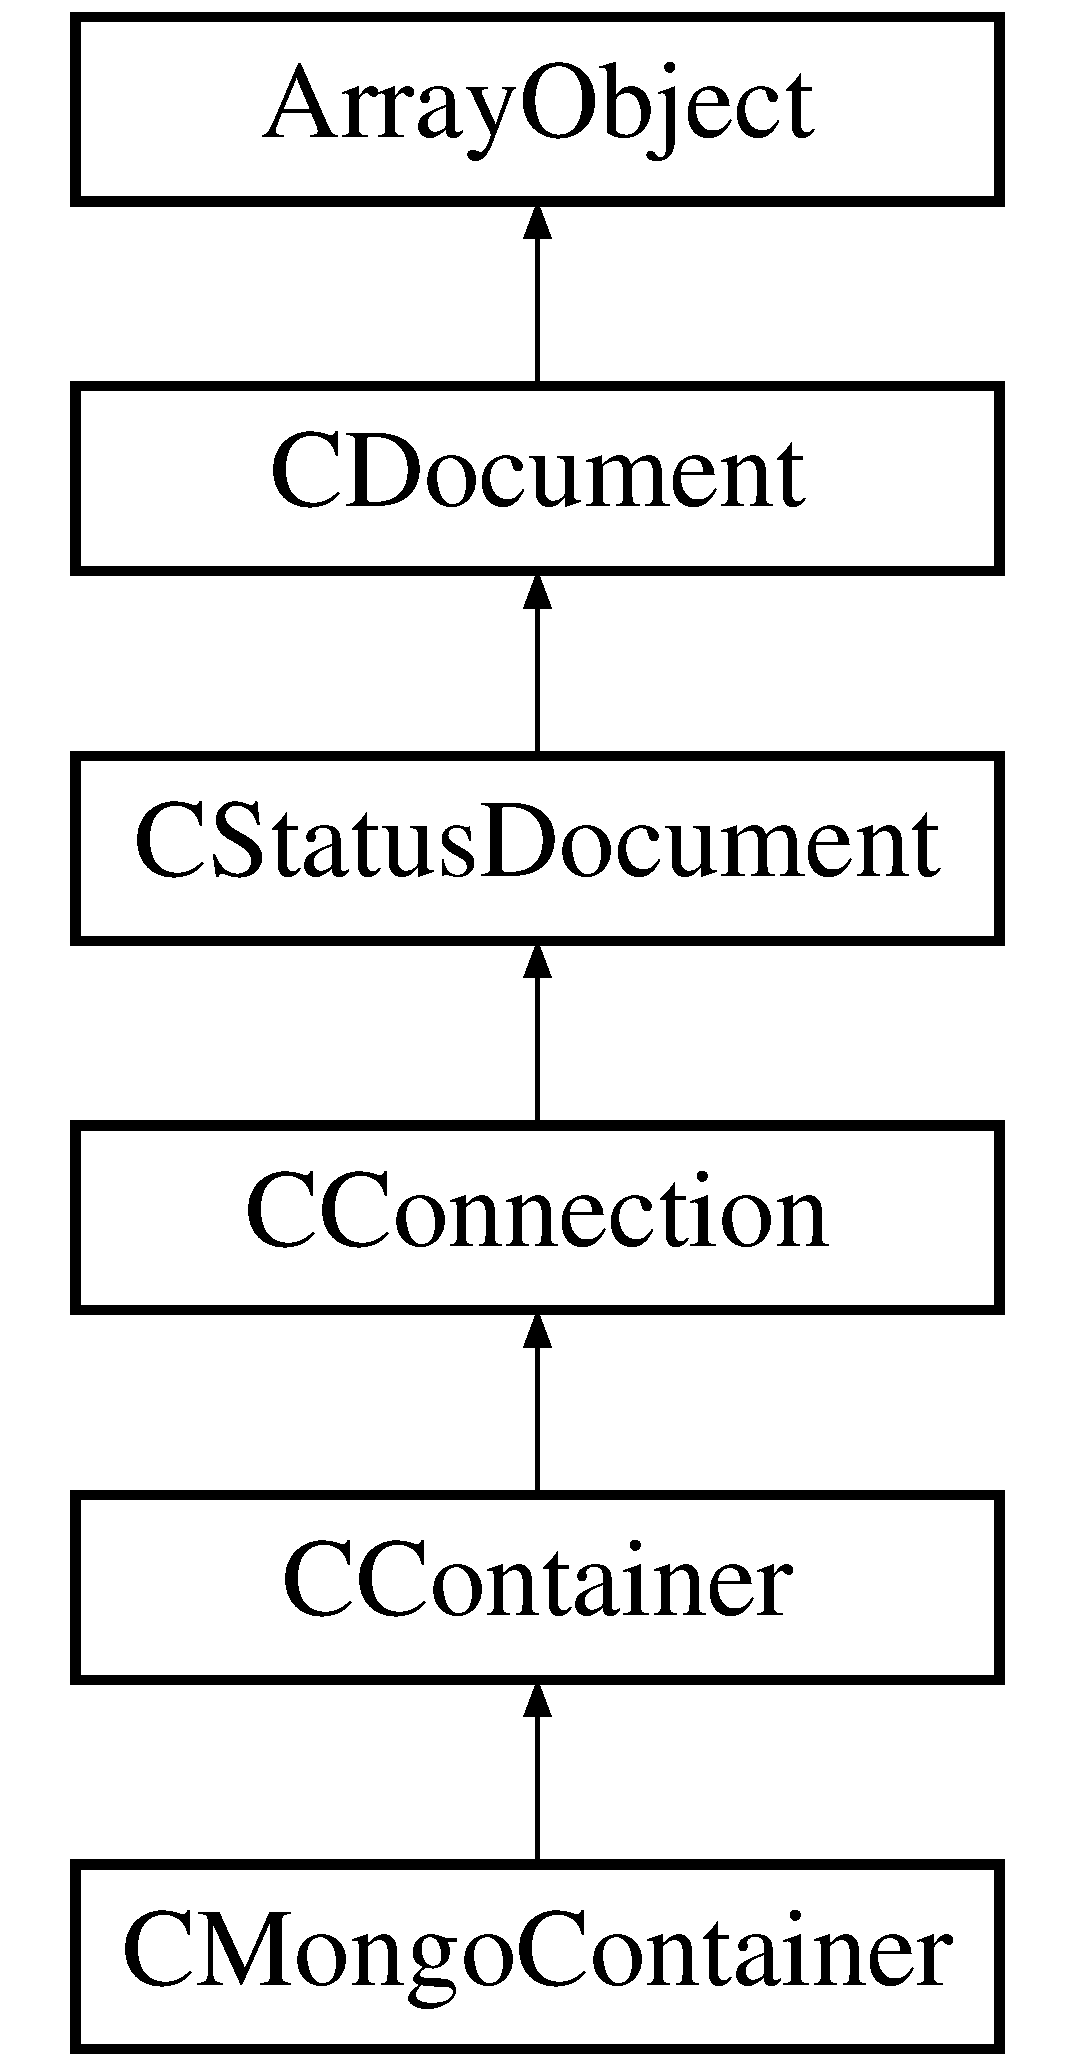
\includegraphics[height=6.000000cm]{class_c_mongo_container}
\end{center}
\end{figure}
\subsection*{Public Member Functions}
\begin{DoxyCompactItemize}
\item 
\hyperlink{class_c_mongo_container_aa2d654b7d2fdddbcb62c52fc8544bb58}{\-\_\-\-\_\-construct} (\$the\-Connection=N\-U\-L\-L, \$the\-Options=N\-U\-L\-L)
\item 
\hyperlink{class_c_mongo_container_abc325eae251667da577efdb45a7d3c17}{\-\_\-\-\_\-to\-String} ()
\item 
\hyperlink{class_c_mongo_container_af3902402e22a90dfcc028b5cfe3eb2e2}{Connection} (\$the\-Value=N\-U\-L\-L, \$get\-Old=F\-A\-L\-S\-E)
\item 
\hyperlink{class_c_mongo_container_a4eecd91ff10c3f0b012f61a02c049019}{Drop} ()
\item 
\hyperlink{class_c_mongo_container_a8931f51d68e4b7a522808d752b582ba5}{Add\-Index} (\$the\-Index, \$the\-Options=Array())
\item 
\hyperlink{class_c_mongo_container_a7fdadf59d9fb17c56a044353cf4bdff0}{Manage\-Object} (\&\$the\-Object, \$the\-Identifier=N\-U\-L\-L, \$the\-Modifiers=k\-F\-L\-A\-G\-\_\-\-D\-E\-F\-A\-U\-L\-T)
\item 
\hyperlink{class_c_mongo_container_a3c173dfe475cefc0c06c834ac0e2e524}{Check\-Object} (\$the\-Identifier, \$the\-Offset=N\-U\-L\-L)
\item 
\hyperlink{class_c_mongo_container_aba1884d8719bb9107250c3d43b7798b3}{Query} (\$the\-Query=N\-U\-L\-L, \$the\-Fields=N\-U\-L\-L, \$the\-Sort=N\-U\-L\-L, \$the\-Start=N\-U\-L\-L, \$the\-Limit=N\-U\-L\-L, \$the\-Result=N\-U\-L\-L)
\item 
\hyperlink{class_c_mongo_container_a7cf34a5efd5dbccffaaf2d2522b1ffcf}{Remove} (\$the\-Query=N\-U\-L\-L)
\item 
\hyperlink{class_c_mongo_container_a644b31ce3fe646dccb3d77e9bc13194e}{Next\-Sequence} (\$the\-Key, \$the\-Container=N\-U\-L\-L)
\item 
\hyperlink{class_c_mongo_container_a35906d30526846445ed8388f33102752}{Unserialise\-Data} (\&\$the\-Element, \$the\-Type=N\-U\-L\-L)
\end{DoxyCompactItemize}
\subsection*{Static Public Member Functions}
\begin{DoxyCompactItemize}
\item 
static \hyperlink{class_c_mongo_container_a01c2948c6d1c9be612a70cc6739def52}{New\-Query} (\$the\-Query=N\-U\-L\-L)
\end{DoxyCompactItemize}
\subsection*{Additional Inherited Members}


\subsection{Constructor \& Destructor Documentation}
\hypertarget{class_c_mongo_container_aa2d654b7d2fdddbcb62c52fc8544bb58}{\index{C\-Mongo\-Container@{C\-Mongo\-Container}!\-\_\-\-\_\-construct@{\-\_\-\-\_\-construct}}
\index{\-\_\-\-\_\-construct@{\-\_\-\-\_\-construct}!CMongoContainer@{C\-Mongo\-Container}}
\subsubsection[{\-\_\-\-\_\-construct}]{\setlength{\rightskip}{0pt plus 5cm}C\-Mongo\-Container\-::\-\_\-\-\_\-construct (
\begin{DoxyParamCaption}
\item[{}]{\$the\-Connection = {\ttfamily NULL}, }
\item[{}]{\$the\-Options = {\ttfamily NULL}}
\end{DoxyParamCaption}
)}}\label{class_c_mongo_container_aa2d654b7d2fdddbcb62c52fc8544bb58}
\subparagraph*{Instantiate class}

The method accepts the same parameters as the \hyperlink{}{Mongo\-Collection} constructor, the first one represents the database object, the second represents the container name, if the latter is missing, the method will raise an exception.

The method will also accept a database object in the first parameter, in that case the second parameter will be ignored.

The method will first attempt to instantiate the \hyperlink{}{Mongo\-Collection} object, it will then store it in the connection data member.


\begin{DoxyParams}[1]{Parameters}
mixed & {\em \$the\-Connection} & Server or database. \\
\hline
mixed & {\em \$the\-Options} & Database name.\\
\hline
\end{DoxyParams}
public

\hyperlink{class_c_mongo_container_af3902402e22a90dfcc028b5cfe3eb2e2}{Connection()} 

\subsection{Member Function Documentation}
\hypertarget{class_c_mongo_container_abc325eae251667da577efdb45a7d3c17}{\index{C\-Mongo\-Container@{C\-Mongo\-Container}!\-\_\-\-\_\-to\-String@{\-\_\-\-\_\-to\-String}}
\index{\-\_\-\-\_\-to\-String@{\-\_\-\-\_\-to\-String}!CMongoContainer@{C\-Mongo\-Container}}
\subsubsection[{\-\_\-\-\_\-to\-String}]{\setlength{\rightskip}{0pt plus 5cm}C\-Mongo\-Container\-::\-\_\-\-\_\-to\-String (
\begin{DoxyParamCaption}
{}
\end{DoxyParamCaption}
)}}\label{class_c_mongo_container_abc325eae251667da577efdb45a7d3c17}
\subparagraph*{Return container name}

This method should return the current container's name.

In this class we return the collection name.

public \begin{DoxyReturn}{Returns}
string The container name.
\end{DoxyReturn}
\hyperlink{class_c_mongo_container_af3902402e22a90dfcc028b5cfe3eb2e2}{Connection()} \hypertarget{class_c_mongo_container_a8931f51d68e4b7a522808d752b582ba5}{\index{C\-Mongo\-Container@{C\-Mongo\-Container}!Add\-Index@{Add\-Index}}
\index{Add\-Index@{Add\-Index}!CMongoContainer@{C\-Mongo\-Container}}
\subsubsection[{Add\-Index}]{\setlength{\rightskip}{0pt plus 5cm}C\-Mongo\-Container\-::\-Add\-Index (
\begin{DoxyParamCaption}
\item[{}]{\$the\-Index, }
\item[{}]{\$the\-Options = {\ttfamily Array()}}
\end{DoxyParamCaption}
)}}\label{class_c_mongo_container_a8931f51d68e4b7a522808d752b582ba5}
\subparagraph*{Add an index}

In this class we simply pass the parameter to the Mongo\-Collection.


\begin{DoxyParams}[1]{Parameters}
array & {\em \$the\-Index} & Key/\-Sort list. \\
\hline
array & {\em \$the\-Options} & List of index options.\\
\hline
\end{DoxyParams}
public \hypertarget{class_c_mongo_container_a3c173dfe475cefc0c06c834ac0e2e524}{\index{C\-Mongo\-Container@{C\-Mongo\-Container}!Check\-Object@{Check\-Object}}
\index{Check\-Object@{Check\-Object}!CMongoContainer@{C\-Mongo\-Container}}
\subsubsection[{Check\-Object}]{\setlength{\rightskip}{0pt plus 5cm}C\-Mongo\-Container\-::\-Check\-Object (
\begin{DoxyParamCaption}
\item[{}]{\$the\-Identifier, }
\item[{}]{\$the\-Offset = {\ttfamily NULL}}
\end{DoxyParamCaption}
)}}\label{class_c_mongo_container_a3c173dfe475cefc0c06c834ac0e2e524}
\subparagraph*{Check if object exists in container}

In this class we return the number of found objects.


\begin{DoxyParams}[1]{Parameters}
mixed & {\em \$the\-Identifier} & Identifier. \\
\hline
string & {\em \$the\-Offset} & Offset.\\
\hline
\end{DoxyParams}
public \begin{DoxyReturn}{Returns}
boolean {\ttfamily T\-R\-U\-E} exists.
\end{DoxyReturn}

\begin{DoxyExceptions}{Exceptions}
{\em Exception} & \hyperlink{class_c_mongo_container_af3902402e22a90dfcc028b5cfe3eb2e2}{Connection()} \\
\hline
\end{DoxyExceptions}
\hypertarget{class_c_mongo_container_af3902402e22a90dfcc028b5cfe3eb2e2}{\index{C\-Mongo\-Container@{C\-Mongo\-Container}!Connection@{Connection}}
\index{Connection@{Connection}!CMongoContainer@{C\-Mongo\-Container}}
\subsubsection[{Connection}]{\setlength{\rightskip}{0pt plus 5cm}C\-Mongo\-Container\-::\-Connection (
\begin{DoxyParamCaption}
\item[{}]{\$the\-Value = {\ttfamily NULL}, }
\item[{}]{\$get\-Old = {\ttfamily FALSE}}
\end{DoxyParamCaption}
)}}\label{class_c_mongo_container_af3902402e22a90dfcc028b5cfe3eb2e2}
\subparagraph*{Manage native connection}

We overload this method to ensure that the provided container is a \hyperlink{}{Mongo\-Collection} object.


\begin{DoxyParams}[1]{Parameters}
mixed & {\em \$the\-Value} & Persistent container or operation. \\
\hline
boolean & {\em \$get\-Old} & {\ttfamily T\-R\-U\-E} get old value.\\
\hline
\end{DoxyParams}
public \begin{DoxyReturn}{Returns}
mixed {\itshape New} or {\itshape old} native container.
\end{DoxyReturn}

\begin{DoxyExceptions}{Exceptions}
{\em Exception} & \\
\hline
\end{DoxyExceptions}
\hypertarget{class_c_mongo_container_a4eecd91ff10c3f0b012f61a02c049019}{\index{C\-Mongo\-Container@{C\-Mongo\-Container}!Drop@{Drop}}
\index{Drop@{Drop}!CMongoContainer@{C\-Mongo\-Container}}
\subsubsection[{Drop}]{\setlength{\rightskip}{0pt plus 5cm}C\-Mongo\-Container\-::\-Drop (
\begin{DoxyParamCaption}
{}
\end{DoxyParamCaption}
)}}\label{class_c_mongo_container_a4eecd91ff10c3f0b012f61a02c049019}
\subparagraph*{Delete a container}

In this class we drop the collection.

public \hypertarget{class_c_mongo_container_a7fdadf59d9fb17c56a044353cf4bdff0}{\index{C\-Mongo\-Container@{C\-Mongo\-Container}!Manage\-Object@{Manage\-Object}}
\index{Manage\-Object@{Manage\-Object}!CMongoContainer@{C\-Mongo\-Container}}
\subsubsection[{Manage\-Object}]{\setlength{\rightskip}{0pt plus 5cm}C\-Mongo\-Container\-::\-Manage\-Object (
\begin{DoxyParamCaption}
\item[{\&}]{\$the\-Object, }
\item[{}]{\$the\-Identifier = {\ttfamily NULL}, }
\item[{}]{\$the\-Modifiers = {\ttfamily kFLAG\-\_\-DEFAULT}}
\end{DoxyParamCaption}
)}}\label{class_c_mongo_container_a7fdadf59d9fb17c56a044353cf4bdff0}
\subparagraph*{Manage an object from the container}

We implement this method to handle Mongo\-Collection object stores.

For more information see \hyperlink{class_c_container_ae2a912b433ba916ce5af0b21d657243b}{C\-Container\-::\-Manage\-Object()}.

{\itshape Note\-: the commit operations are performed by default with the default Mongo {\ttfamily Write\-Concerns} option.}


\begin{DoxyParams}[1]{Parameters}
reference & {\em \&\$the\-Object} & Object. \\
\hline
mixed & {\em \$the\-Identifier} & Identifier. \\
\hline
mixed & {\em \$the\-Modifiers} & Options or offsets list.\\
\hline
\end{DoxyParams}
public \begin{DoxyReturn}{Returns}
mixed The native operation status.
\end{DoxyReturn}

\begin{DoxyExceptions}{Exceptions}
{\em Exception} & \hyperlink{class_c_mongo_container_af3902402e22a90dfcc028b5cfe3eb2e2}{Connection()}\\
\hline
\end{DoxyExceptions}
\begin{DoxySeeAlso}{See Also}
k\-F\-L\-A\-G\-\_\-\-P\-E\-R\-S\-I\-S\-T\-\_\-\-M\-A\-S\-K k\-F\-L\-A\-G\-\_\-\-P\-E\-R\-S\-I\-S\-T\-\_\-\-I\-N\-S\-E\-R\-T k\-F\-L\-A\-G\-\_\-\-P\-E\-R\-S\-I\-S\-T\-\_\-\-U\-P\-D\-A\-T\-E 

k\-F\-L\-A\-G\-\_\-\-P\-E\-R\-S\-I\-S\-T\-\_\-\-R\-E\-P\-L\-A\-C\-E k\-F\-L\-A\-G\-\_\-\-P\-E\-R\-S\-I\-S\-T\-\_\-\-M\-O\-D\-I\-F\-Y k\-F\-L\-A\-G\-\_\-\-P\-E\-R\-S\-I\-S\-T\-\_\-\-D\-E\-L\-E\-T\-E 
\end{DoxySeeAlso}
\hypertarget{class_c_mongo_container_a01c2948c6d1c9be612a70cc6739def52}{\index{C\-Mongo\-Container@{C\-Mongo\-Container}!New\-Query@{New\-Query}}
\index{New\-Query@{New\-Query}!CMongoContainer@{C\-Mongo\-Container}}
\subsubsection[{New\-Query}]{\setlength{\rightskip}{0pt plus 5cm}static C\-Mongo\-Container\-::\-New\-Query (
\begin{DoxyParamCaption}
\item[{}]{\$the\-Query = {\ttfamily NULL}}
\end{DoxyParamCaption}
)\hspace{0.3cm}{\ttfamily [static]}}}\label{class_c_mongo_container_a01c2948c6d1c9be612a70cc6739def52}
\subparagraph*{Return an empty query}

In this class we return an empty \hyperlink{class_c_mongo_query}{C\-Mongo\-Query} instance.


\begin{DoxyParams}[1]{Parameters}
mixed & {\em \$the\-Query} & Query data.\\
\hline
\end{DoxyParams}
\begin{DoxyReturn}{Returns}
\hyperlink{class_c_query}{C\-Query} An empty query object. 
\end{DoxyReturn}
\hypertarget{class_c_mongo_container_a644b31ce3fe646dccb3d77e9bc13194e}{\index{C\-Mongo\-Container@{C\-Mongo\-Container}!Next\-Sequence@{Next\-Sequence}}
\index{Next\-Sequence@{Next\-Sequence}!CMongoContainer@{C\-Mongo\-Container}}
\subsubsection[{Next\-Sequence}]{\setlength{\rightskip}{0pt plus 5cm}C\-Mongo\-Container\-::\-Next\-Sequence (
\begin{DoxyParamCaption}
\item[{}]{\$the\-Key, }
\item[{}]{\$the\-Container = {\ttfamily NULL}}
\end{DoxyParamCaption}
)}}\label{class_c_mongo_container_a644b31ce3fe646dccb3d77e9bc13194e}
\subparagraph*{Return a sequence number}

We overload this method here to implement sequence numbers in mongo containers, please refer to the \hyperlink{class_c_container_afa72f0da28ad8c3955cb9fedbc0ac2df}{C\-Container\-::\-Next\-Sequence()} documentation for more information.


\begin{DoxyParams}[1]{Parameters}
string & {\em \$the\-Key} & Sequence key. \\
\hline
mixed & {\em \$the\-Container} & Sequence container.\\
\hline
\end{DoxyParams}
public \begin{DoxyReturn}{Returns}
mixed The sequence number or {\ttfamily N\-U\-L\-L}.
\end{DoxyReturn}

\begin{DoxyExceptions}{Exceptions}
{\em Exception} & \\
\hline
\end{DoxyExceptions}
\hypertarget{class_c_mongo_container_aba1884d8719bb9107250c3d43b7798b3}{\index{C\-Mongo\-Container@{C\-Mongo\-Container}!Query@{Query}}
\index{Query@{Query}!CMongoContainer@{C\-Mongo\-Container}}
\subsubsection[{Query}]{\setlength{\rightskip}{0pt plus 5cm}C\-Mongo\-Container\-::\-Query (
\begin{DoxyParamCaption}
\item[{}]{\$the\-Query = {\ttfamily NULL}, }
\item[{}]{\$the\-Fields = {\ttfamily NULL}, }
\item[{}]{\$the\-Sort = {\ttfamily NULL}, }
\item[{}]{\$the\-Start = {\ttfamily NULL}, }
\item[{}]{\$the\-Limit = {\ttfamily NULL}, }
\item[{}]{\$the\-Result = {\ttfamily NULL}}
\end{DoxyParamCaption}
)}}\label{class_c_mongo_container_aba1884d8719bb9107250c3d43b7798b3}
\subparagraph*{Perform a query}

This method will perform the provided query on the current container, please refer to the \hyperlink{class_c_container_a9f422d5c6d99eea28993614749ee05a3}{C\-Container\-::\-Query()} reference for more information.


\begin{DoxyParams}[1]{Parameters}
array & {\em \$the\-Query} & Query. \\
\hline
array & {\em \$the\-Fields} & Fields set. \\
\hline
array & {\em \$the\-Sort} & Sort order. \\
\hline
integer & {\em \$the\-Start} & Page start. \\
\hline
integer & {\em \$the\-Limit} & Page limit. \\
\hline
mixed & {\em \$the\-Result} & Result type.\\
\hline
\end{DoxyParams}
public \begin{DoxyReturn}{Returns}
object Native recordset. 
\end{DoxyReturn}
\hypertarget{class_c_mongo_container_a7cf34a5efd5dbccffaaf2d2522b1ffcf}{\index{C\-Mongo\-Container@{C\-Mongo\-Container}!Remove@{Remove}}
\index{Remove@{Remove}!CMongoContainer@{C\-Mongo\-Container}}
\subsubsection[{Remove}]{\setlength{\rightskip}{0pt plus 5cm}C\-Mongo\-Container\-::\-Remove (
\begin{DoxyParamCaption}
\item[{}]{\$the\-Query = {\ttfamily NULL}}
\end{DoxyParamCaption}
)}}\label{class_c_mongo_container_a7cf34a5efd5dbccffaaf2d2522b1ffcf}
\subparagraph*{Perform a deletion}

In this class we use the default Mongo Write\-Concerns.


\begin{DoxyParams}[1]{Parameters}
array & {\em \$the\-Query} & Query.\\
\hline
\end{DoxyParams}
public \begin{DoxyReturn}{Returns}
integer Number of affected elements. 
\end{DoxyReturn}
\hypertarget{class_c_mongo_container_a35906d30526846445ed8388f33102752}{\index{C\-Mongo\-Container@{C\-Mongo\-Container}!Unserialise\-Data@{Unserialise\-Data}}
\index{Unserialise\-Data@{Unserialise\-Data}!CMongoContainer@{C\-Mongo\-Container}}
\subsubsection[{Unserialise\-Data}]{\setlength{\rightskip}{0pt plus 5cm}C\-Mongo\-Container\-::\-Unserialise\-Data (
\begin{DoxyParamCaption}
\item[{\&}]{\$the\-Element, }
\item[{}]{\$the\-Type = {\ttfamily NULL}}
\end{DoxyParamCaption}
)}}\label{class_c_mongo_container_a35906d30526846445ed8388f33102752}
Unserialise provided data element.

This method should convert the provided structure into a custom data type compatible with the current container.

This method is called by a public \hyperlink{class_c_container_aa339d3c4c9b011713176a89fe9c7783d}{Unserialise\-Object()} interface which traverses an object and provides this method with all elements that satisfy the following conditions\-:


\begin{DoxyItemize}
\item {\ttfamily \hyperlink{class_c_data_type}{C\-Data\-Type}}\-: All instances derived from this class are sent to this method. 
\item {\ttfamily Array} or {\ttfamily Array\-Object}\-: If the structure is composed of exactly two offsets and these elements are \hyperlink{}{k\-T\-A\-G\-\_\-\-C\-U\-S\-T\-O\-M\-\_\-\-T\-Y\-P\-E} and \hyperlink{}{k\-T\-A\-G\-\_\-\-C\-U\-S\-T\-O\-M\-\_\-\-D\-A\-T\-A}, it will be sent to this method. 
\end{DoxyItemize}

In this class we parse the following types and offsets\-:


\begin{DoxyItemize}
\item {\itshape \hyperlink{class_c_data_type_mongo_id}{C\-Data\-Type\-Mongo\-Id} object or \hyperlink{}{k\-T\-Y\-P\-E\-\_\-\-Mongo\-Id} offset}\-: We return a Mongo\-Id object. 
\item {\itshape \hyperlink{class_c_data_type_mongo_code}{C\-Data\-Type\-Mongo\-Code} object or \hyperlink{}{k\-T\-Y\-P\-E\-\_\-\-Mongo\-Code} offset}\-: We return a Mongo\-Code object. 
\item {\itshape \hyperlink{class_c_data_type_stamp}{C\-Data\-Type\-Stamp} object or \hyperlink{}{k\-T\-Y\-P\-E\-\_\-\-S\-T\-A\-M\-P} offset}\-: We return a Mongo\-Date object. 
\item {\itshape \hyperlink{class_c_data_type_regex}{C\-Data\-Type\-Regex} object or \hyperlink{}{k\-T\-Y\-P\-E\-\_\-\-R\-E\-G\-E\-X\-\_\-\-S\-T\-R\-I\-N\-G} offset}\-: We return a Mongo\-Regex object. 
\item {\itshape \hyperlink{class_c_data_type_int32}{C\-Data\-Type\-Int32} object or \hyperlink{}{k\-T\-Y\-P\-E\-\_\-\-I\-N\-T32} offset}\-: We return a Mongo\-Int32 object. 
\item {\itshape \hyperlink{class_c_data_type_int64}{C\-Data\-Type\-Int64} object or \hyperlink{}{k\-T\-Y\-P\-E\-\_\-\-I\-N\-T64} offset}\-: We return a Mongo\-Int64 object. 
\item {\itshape \hyperlink{class_c_data_type_binary}{C\-Data\-Type\-Binary} object or \hyperlink{}{k\-T\-Y\-P\-E\-\_\-\-B\-I\-N\-A\-R\-Y\-\_\-\-S\-T\-R\-I\-N\-G} offset}\-: We return a Mongo\-Bin\-Data object. 
\end{DoxyItemize}

The elements to be converted are provided by reference, which means that they have to be converted in place.

This method can also be used in a different way\-: you can ask the method to convert the provided scalar to the corresponding Mongo custom type, for this you need to provide a scalar in the first parameter and a data type in the second.


\begin{DoxyParams}[1]{Parameters}
reference & {\em \&\$the\-Element} & Element to encode. \\
\hline
string & {\em \$the\-Type} & Data type.\\
\hline
\end{DoxyParams}
public 

The documentation for this class was generated from the following file\-:\begin{DoxyCompactItemize}
\item 
/\-Library/\-Web\-Server/\-Library/\-P\-H\-P\-Wrapper/classes/C\-Mongo\-Container.\-php\end{DoxyCompactItemize}

\hypertarget{class_c_mongo_database}{\section{C\-Mongo\-Database Class Reference}
\label{class_c_mongo_database}\index{C\-Mongo\-Database@{C\-Mongo\-Database}}
}
Inheritance diagram for C\-Mongo\-Database\-:\begin{figure}[H]
\begin{center}
\leavevmode
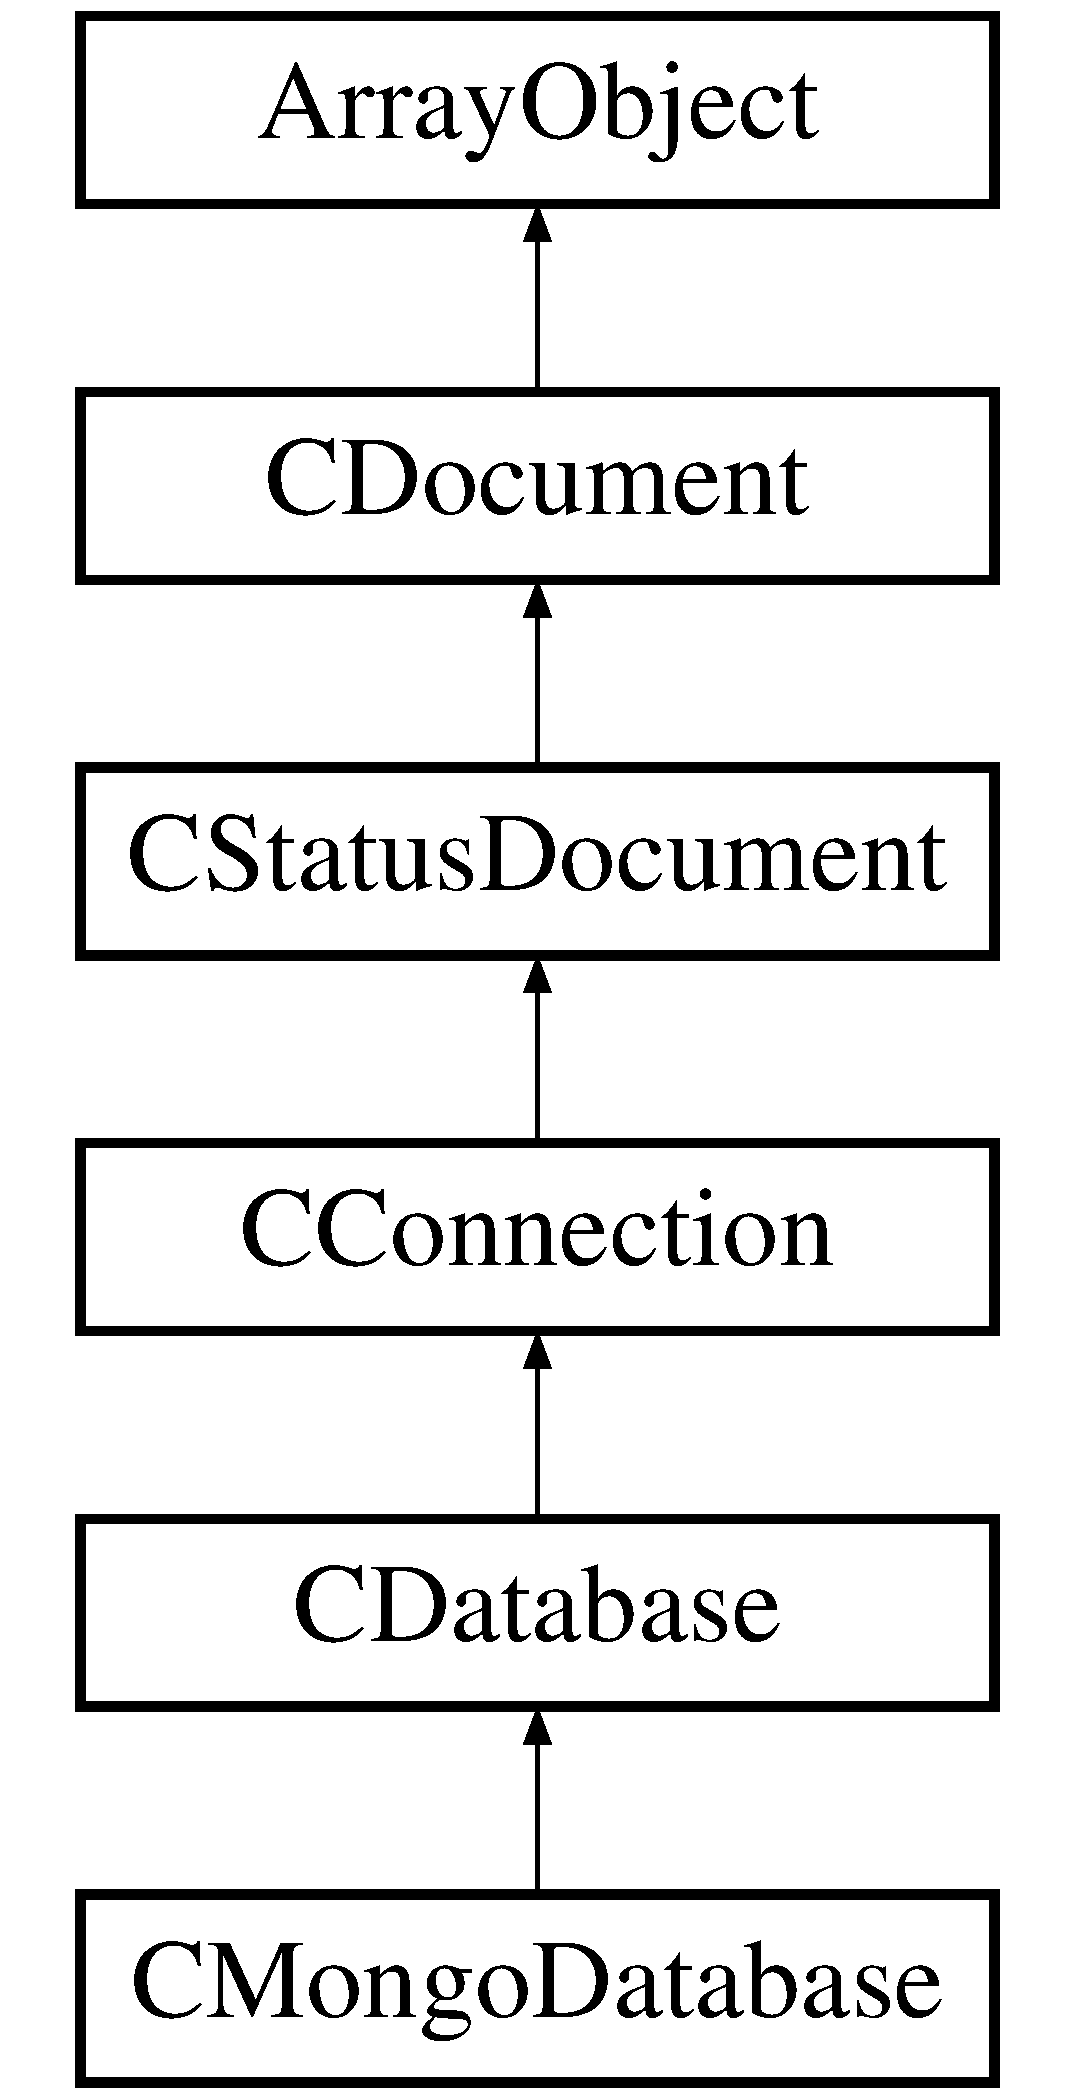
\includegraphics[height=6.000000cm]{class_c_mongo_database}
\end{center}
\end{figure}
\subsection*{Public Member Functions}
\begin{DoxyCompactItemize}
\item 
\hyperlink{class_c_mongo_database_ac9b493d1c9a23cd6d06d4d636e53bd93}{\-\_\-\-\_\-construct} (\$the\-Connection=N\-U\-L\-L, \$the\-Options=N\-U\-L\-L)
\item 
\hyperlink{class_c_mongo_database_aa4a30efd8f5de278647f1232348a4a04}{\-\_\-\-\_\-to\-String} ()
\item 
\hyperlink{class_c_mongo_database_a6df2c2b97dd495d7f2bd30df63ab37ab}{Connection} (\$the\-Value=N\-U\-L\-L, \$get\-Old=F\-A\-L\-S\-E)
\item 
\hyperlink{class_c_mongo_database_ae7f6d6bfbb128c284159cc63ea54ce45}{Drop} ()
\item 
\hyperlink{class_c_mongo_database_a22b8212f2ae256c883ba58140d8fe01a}{Container} (\$the\-Container=N\-U\-L\-L)
\end{DoxyCompactItemize}
\subsection*{Additional Inherited Members}


\subsection{Constructor \& Destructor Documentation}
\hypertarget{class_c_mongo_database_ac9b493d1c9a23cd6d06d4d636e53bd93}{\index{C\-Mongo\-Database@{C\-Mongo\-Database}!\-\_\-\-\_\-construct@{\-\_\-\-\_\-construct}}
\index{\-\_\-\-\_\-construct@{\-\_\-\-\_\-construct}!CMongoDatabase@{C\-Mongo\-Database}}
\subsubsection[{\-\_\-\-\_\-construct}]{\setlength{\rightskip}{0pt plus 5cm}C\-Mongo\-Database\-::\-\_\-\-\_\-construct (
\begin{DoxyParamCaption}
\item[{}]{\$the\-Connection = {\ttfamily NULL}, }
\item[{}]{\$the\-Options = {\ttfamily NULL}}
\end{DoxyParamCaption}
)}}\label{class_c_mongo_database_ac9b493d1c9a23cd6d06d4d636e53bd93}
\subparagraph*{Instantiate class}

The method accepts the same parameters as the \hyperlink{}{Mongo\-D\-B} constructor, the first one represents the server object, the second represents the database name, if the latter is missing, the method will raise an exception.

The method will also accept a server object in the first parameter, in that case the second parameter will be ignored.

The method will first attempt to instantiate the \hyperlink{}{Mongo\-D\-B} object, it will then store it in the connection data member.


\begin{DoxyParams}[1]{Parameters}
mixed & {\em \$the\-Connection} & Server or database. \\
\hline
mixed & {\em \$the\-Options} & Database name.\\
\hline
\end{DoxyParams}
public

\hyperlink{class_c_mongo_database_a6df2c2b97dd495d7f2bd30df63ab37ab}{Connection()} 

\subsection{Member Function Documentation}
\hypertarget{class_c_mongo_database_aa4a30efd8f5de278647f1232348a4a04}{\index{C\-Mongo\-Database@{C\-Mongo\-Database}!\-\_\-\-\_\-to\-String@{\-\_\-\-\_\-to\-String}}
\index{\-\_\-\-\_\-to\-String@{\-\_\-\-\_\-to\-String}!CMongoDatabase@{C\-Mongo\-Database}}
\subsubsection[{\-\_\-\-\_\-to\-String}]{\setlength{\rightskip}{0pt plus 5cm}C\-Mongo\-Database\-::\-\_\-\-\_\-to\-String (
\begin{DoxyParamCaption}
{}
\end{DoxyParamCaption}
)}}\label{class_c_mongo_database_aa4a30efd8f5de278647f1232348a4a04}
\subparagraph*{Return connection name}

In this class the method will return the server's connection U\-R\-L, which corresponds to the \hyperlink{}{k\-O\-F\-F\-S\-E\-T\-\_\-\-N\-A\-M\-E} offset.

public \begin{DoxyReturn}{Returns}
string The connection name. 
\end{DoxyReturn}
\hypertarget{class_c_mongo_database_a6df2c2b97dd495d7f2bd30df63ab37ab}{\index{C\-Mongo\-Database@{C\-Mongo\-Database}!Connection@{Connection}}
\index{Connection@{Connection}!CMongoDatabase@{C\-Mongo\-Database}}
\subsubsection[{Connection}]{\setlength{\rightskip}{0pt plus 5cm}C\-Mongo\-Database\-::\-Connection (
\begin{DoxyParamCaption}
\item[{}]{\$the\-Value = {\ttfamily NULL}, }
\item[{}]{\$get\-Old = {\ttfamily FALSE}}
\end{DoxyParamCaption}
)}}\label{class_c_mongo_database_a6df2c2b97dd495d7f2bd30df63ab37ab}
\subparagraph*{Manage native connection}

We overload this method to ensure the provided value is an instance of \hyperlink{}{Mongo}, if this is not the case, the method will raise an exception.

The method will attempt to parse the provided server U\-R\-L and store the results in the array part of the object. For more information on the parsed elements consult the P\-H\-P \hyperlink{}{parse\-\_\-url()} function.

Although the database name can be obtained from the native connection, we still store it in the \hyperlink{}{k\-O\-F\-F\-S\-E\-T\-\_\-\-N\-A\-M\-E} offset for consistency with other connection objects.


\begin{DoxyParams}[1]{Parameters}
mixed & {\em \$the\-Value} & Native connection or operation. \\
\hline
boolean & {\em \$get\-Old} & {\ttfamily T\-R\-U\-E} get old value.\\
\hline
\end{DoxyParams}
public \begin{DoxyReturn}{Returns}
mixed {\itshape New} or {\itshape old} native connection.
\end{DoxyReturn}

\begin{DoxyExceptions}{Exceptions}
{\em Exception} & \\
\hline
\end{DoxyExceptions}
\hypertarget{class_c_mongo_database_a22b8212f2ae256c883ba58140d8fe01a}{\index{C\-Mongo\-Database@{C\-Mongo\-Database}!Container@{Container}}
\index{Container@{Container}!CMongoDatabase@{C\-Mongo\-Database}}
\subsubsection[{Container}]{\setlength{\rightskip}{0pt plus 5cm}C\-Mongo\-Database\-::\-Container (
\begin{DoxyParamCaption}
\item[{}]{\$the\-Container = {\ttfamily NULL}}
\end{DoxyParamCaption}
)}}\label{class_c_mongo_database_a22b8212f2ae256c883ba58140d8fe01a}
\subparagraph*{Generate a container object}

In this class we return \hyperlink{class_c_mongo_container}{C\-Mongo\-Container} instances, the provided parameter is interpreted as the container name.

If you omit the parameter, the method will raise an exception, in derived classes you can overload the method to provide a default container name.

If the object does not have its native connection, the method will also raise an exception.


\begin{DoxyParams}[1]{Parameters}
string & {\em \$the\-Container} & Container name.\\
\hline
\end{DoxyParams}
public \begin{DoxyReturn}{Returns}
mixed The container object.
\end{DoxyReturn}

\begin{DoxyExceptions}{Exceptions}
{\em Exception} & \hyperlink{class_c_status_document_a954dee06e219e0a0f2e7fa6edac56e28}{\-\_\-\-Is\-Inited()} \\
\hline
\end{DoxyExceptions}
\hypertarget{class_c_mongo_database_ae7f6d6bfbb128c284159cc63ea54ce45}{\index{C\-Mongo\-Database@{C\-Mongo\-Database}!Drop@{Drop}}
\index{Drop@{Drop}!CMongoDatabase@{C\-Mongo\-Database}}
\subsubsection[{Drop}]{\setlength{\rightskip}{0pt plus 5cm}C\-Mongo\-Database\-::\-Drop (
\begin{DoxyParamCaption}
{}
\end{DoxyParamCaption}
)}}\label{class_c_mongo_database_ae7f6d6bfbb128c284159cc63ea54ce45}
\subparagraph*{Delete a database}

In this class we drop the database.

public 

The documentation for this class was generated from the following file\-:\begin{DoxyCompactItemize}
\item 
/\-Library/\-Web\-Server/\-Library/\-P\-H\-P\-Wrapper/classes/C\-Mongo\-Database.\-php\end{DoxyCompactItemize}

\hypertarget{class_c_mongo_query}{\section{C\-Mongo\-Query Class Reference}
\label{class_c_mongo_query}\index{C\-Mongo\-Query@{C\-Mongo\-Query}}
}
Inheritance diagram for C\-Mongo\-Query\-:\begin{figure}[H]
\begin{center}
\leavevmode
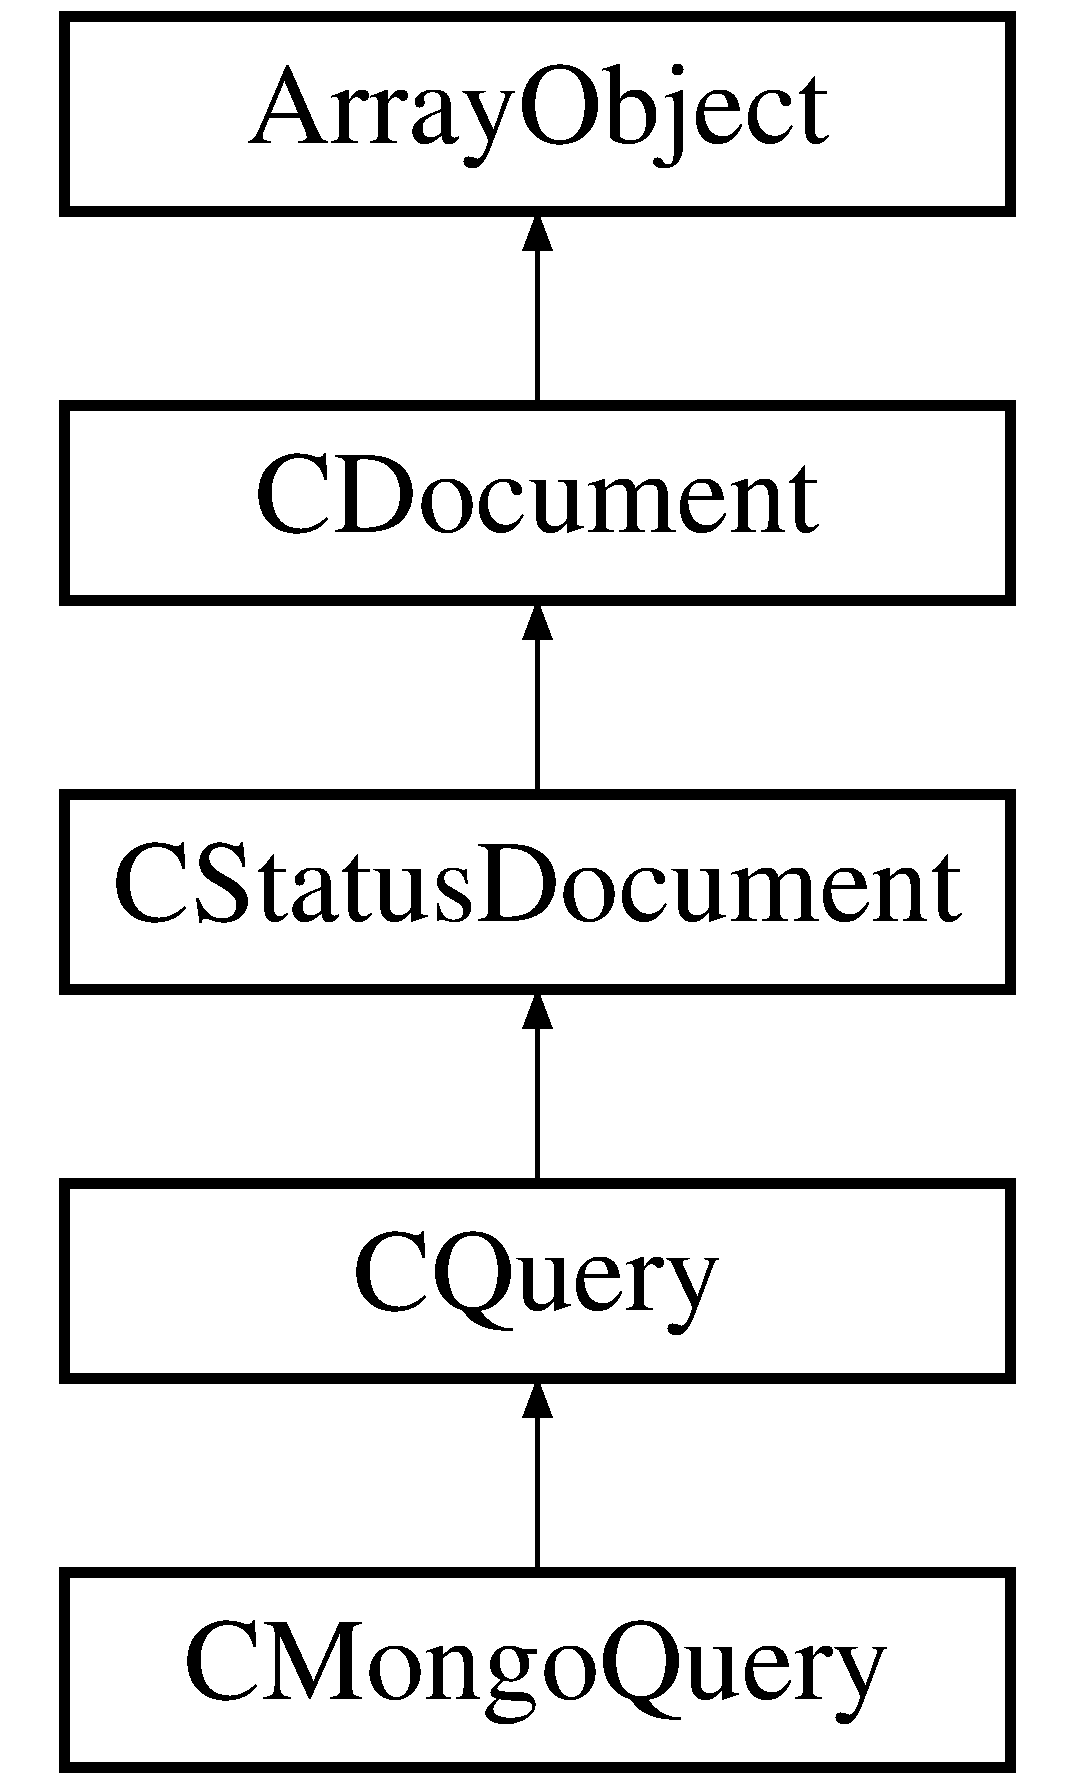
\includegraphics[height=5.000000cm]{class_c_mongo_query}
\end{center}
\end{figure}
\subsection*{Public Member Functions}
\begin{DoxyCompactItemize}
\item 
\hyperlink{class_c_mongo_query_a8fb40265adf169720a6f175212ef6b09}{Export} (\hyperlink{class_c_connection}{C\-Connection} \$the\-Container)
\end{DoxyCompactItemize}
\subsection*{Protected Member Functions}
\begin{DoxyCompactItemize}
\item 
\hyperlink{class_c_mongo_query_a651af70656cb9894ef1885a711a0c141}{\-\_\-\-Validate\-Condition} (\$the\-Condition, \$the\-Statements, \$the\-Level)
\item 
\hyperlink{class_c_mongo_query_a8cda9306ac308f5c33456e77de004ebb}{\-\_\-\-Convert\-Condition} (\&\$the\-Query, \$the\-Container, \$the\-Condition, \$the\-Statements)
\item 
\hyperlink{class_c_mongo_query_a1f381db3f898f4c9cd333ffd2e3e989b}{\-\_\-\-Convert\-Statement} (\&\$the\-Query, \$the\-Container, \$the\-Condition, \$the\-Statement)
\item 
\hyperlink{class_c_mongo_query_a32fd372e1c39add42d078441eda3f1c3}{\-\_\-\-Order\-Range} (\$the\-Range, \hyperlink{class_c_mongo_container}{C\-Mongo\-Container} \$the\-Container, \$the\-Type)
\end{DoxyCompactItemize}
\subsection*{Additional Inherited Members}


\subsection{Member Function Documentation}
\hypertarget{class_c_mongo_query_a8cda9306ac308f5c33456e77de004ebb}{\index{C\-Mongo\-Query@{C\-Mongo\-Query}!\-\_\-\-Convert\-Condition@{\-\_\-\-Convert\-Condition}}
\index{\-\_\-\-Convert\-Condition@{\-\_\-\-Convert\-Condition}!CMongoQuery@{C\-Mongo\-Query}}
\subsubsection[{\-\_\-\-Convert\-Condition}]{\setlength{\rightskip}{0pt plus 5cm}C\-Mongo\-Query\-::\-\_\-\-Convert\-Condition (
\begin{DoxyParamCaption}
\item[{\&}]{\$the\-Query, }
\item[{}]{\$the\-Container, }
\item[{}]{\$the\-Condition, }
\item[{}]{\$the\-Statements}
\end{DoxyParamCaption}
)\hspace{0.3cm}{\ttfamily [protected]}}}\label{class_c_mongo_query_a8cda9306ac308f5c33456e77de004ebb}
\subparagraph*{Convert condition}

This method will convert the provided condition block into a Mongo compatible condition block, it is called by the \hyperlink{class_c_mongo_query_a8fb40265adf169720a6f175212ef6b09}{Export()} method or called recursively to convert embedded conditions.

The method expects the following parameters\-:


\begin{DoxyItemize}
\item {\ttfamily \&\$the\-Query}\-: Reference to an array that will receive the converted condition. 
\item {\ttfamily \$the\-Container}\-: Data container, must be derived from \hyperlink{class_c_mongo_container}{C\-Mongo\-Container}. 
\item {\ttfamily \$the\-Condition}\-: Boolean condition code. 
\item {\ttfamily \$the\-Statements}\-: List of condition statements. 
\end{DoxyItemize}


\begin{DoxyParams}[1]{Parameters}
reference & {\em \&\$the\-Query} & Receives converted query. \\
\hline
\hyperlink{class_c_mongo_container}{C\-Mongo\-Container} & {\em \$the\-Container} & Query container. \\
\hline
string & {\em \$the\-Condition} & Boolean condition. \\
\hline
array & {\em \$the\-Statements} & Statements list.\\
\hline
\end{DoxyParams}
protected \hypertarget{class_c_mongo_query_a1f381db3f898f4c9cd333ffd2e3e989b}{\index{C\-Mongo\-Query@{C\-Mongo\-Query}!\-\_\-\-Convert\-Statement@{\-\_\-\-Convert\-Statement}}
\index{\-\_\-\-Convert\-Statement@{\-\_\-\-Convert\-Statement}!CMongoQuery@{C\-Mongo\-Query}}
\subsubsection[{\-\_\-\-Convert\-Statement}]{\setlength{\rightskip}{0pt plus 5cm}C\-Mongo\-Query\-::\-\_\-\-Convert\-Statement (
\begin{DoxyParamCaption}
\item[{\&}]{\$the\-Query, }
\item[{}]{\$the\-Container, }
\item[{}]{\$the\-Condition, }
\item[{}]{\$the\-Statement}
\end{DoxyParamCaption}
)\hspace{0.3cm}{\ttfamily [protected]}}}\label{class_c_mongo_query_a1f381db3f898f4c9cd333ffd2e3e989b}
\subparagraph*{Convert statement}

This method can be used to convert a condition statement to a Mongo compatible statement, it is called by the \hyperlink{class_c_mongo_query_a8cda9306ac308f5c33456e77de004ebb}{\-\_\-\-Convert\-Condition()} method which feeds it each element of the condition block.

The method expects the following parameters\-:


\begin{DoxyItemize}
\item {\ttfamily \&\$the\-Query}\-: Reference to an array that will receive the converted statement. 
\item {\ttfamily \$the\-Container}\-: Data container, must be derived from \hyperlink{class_c_mongo_container}{C\-Mongo\-Container} and we assume this check has been done by the caller. 
\item {\ttfamily \$the\-Condition}\-: Boolean condition code. 
\item {\ttfamily \$the\-Statement}\-: Statement or embedded condition. 
\end{DoxyItemize}

Note that this method will recursively call \hyperlink{class_c_mongo_query_a8cda9306ac308f5c33456e77de004ebb}{\-\_\-\-Convert\-Condition()} if the current element of the provided statement is a condition code\-: this means that the element is a nested condition.


\begin{DoxyParams}[1]{Parameters}
reference & {\em \&\$the\-Query} & Receives converted statement. \\
\hline
\hyperlink{class_c_mongo_container}{C\-Mongo\-Container} & {\em \$the\-Container} & Query container. \\
\hline
string & {\em \$the\-Condition} & Boolean condition. \\
\hline
array & {\em \$the\-Statement} & Statement.\\
\hline
\end{DoxyParams}
protected \hypertarget{class_c_mongo_query_a32fd372e1c39add42d078441eda3f1c3}{\index{C\-Mongo\-Query@{C\-Mongo\-Query}!\-\_\-\-Order\-Range@{\-\_\-\-Order\-Range}}
\index{\-\_\-\-Order\-Range@{\-\_\-\-Order\-Range}!CMongoQuery@{C\-Mongo\-Query}}
\subsubsection[{\-\_\-\-Order\-Range}]{\setlength{\rightskip}{0pt plus 5cm}C\-Mongo\-Query\-::\-\_\-\-Order\-Range (
\begin{DoxyParamCaption}
\item[{}]{\$the\-Range, }
\item[{{\bf C\-Mongo\-Container}}]{\$the\-Container, }
\item[{}]{\$the\-Type}
\end{DoxyParamCaption}
)\hspace{0.3cm}{\ttfamily [protected]}}}\label{class_c_mongo_query_a32fd372e1c39add42d078441eda3f1c3}
\subparagraph*{Order range elements}

This method will order the provided range elements, the method accepts an array of two elements which represent the range bounds and will return an array with the two provided elements sorted.

The method accepts three parameters\-:


\begin{DoxyItemize}
\item {\ttfamily \$the\-Range}\-: An array containing two elements representing the range bounds. 
\item {\ttfamily \$the\-Container}\-: The \hyperlink{class_c_mongo_container}{C\-Mongo\-Container} on which the query will be executed. 
\item {\ttfamily \$the\-Type}\-: The data type of the range elements. 
\end{DoxyItemize}


\begin{DoxyParams}[1]{Parameters}
mixed & {\em \$the\-Range} & Range elements. \\
\hline
\hyperlink{class_c_mongo_container}{C\-Mongo\-Container} & {\em \$the\-Container} & Query container. \\
\hline
string & {\em \$the\-Type} & Elements data type.\\
\hline
\end{DoxyParams}
protected \begin{DoxyReturn}{Returns}
array 
\end{DoxyReturn}
\hypertarget{class_c_mongo_query_a651af70656cb9894ef1885a711a0c141}{\index{C\-Mongo\-Query@{C\-Mongo\-Query}!\-\_\-\-Validate\-Condition@{\-\_\-\-Validate\-Condition}}
\index{\-\_\-\-Validate\-Condition@{\-\_\-\-Validate\-Condition}!CMongoQuery@{C\-Mongo\-Query}}
\subsubsection[{\-\_\-\-Validate\-Condition}]{\setlength{\rightskip}{0pt plus 5cm}C\-Mongo\-Query\-::\-\_\-\-Validate\-Condition (
\begin{DoxyParamCaption}
\item[{}]{\$the\-Condition, }
\item[{}]{\$the\-Statements, }
\item[{}]{\$the\-Level}
\end{DoxyParamCaption}
)\hspace{0.3cm}{\ttfamily [protected]}}}\label{class_c_mongo_query_a651af70656cb9894ef1885a711a0c141}
\subparagraph*{Validate condition}

This method expects a condition as its argument, it will check if it is a valid condition, then it will validate all condition statements.

In this class we handle queries to Mongo databases, so the depth of the query conditions cannot go beyond 2 levels.

We overload this method to prevent nesting O\-R conditions.


\begin{DoxyParams}[1]{Parameters}
string & {\em \$the\-Condition} & Boolean condition. \\
\hline
array & {\em \$the\-Statements} & Statements list. \\
\hline
integer & {\em \$the\-Level} & \mbox{[}P\-R\-I\-V\-A\-T\-E\mbox{]} condition level.\\
\hline
\end{DoxyParams}
protected \hypertarget{class_c_mongo_query_a8fb40265adf169720a6f175212ef6b09}{\index{C\-Mongo\-Query@{C\-Mongo\-Query}!Export@{Export}}
\index{Export@{Export}!CMongoQuery@{C\-Mongo\-Query}}
\subsubsection[{Export}]{\setlength{\rightskip}{0pt plus 5cm}C\-Mongo\-Query\-::\-Export (
\begin{DoxyParamCaption}
\item[{{\bf C\-Connection}}]{\$the\-Container}
\end{DoxyParamCaption}
)}}\label{class_c_mongo_query_a8fb40265adf169720a6f175212ef6b09}
\subparagraph*{Export query}

We overload the inherited method to generate Mongo specific queries.

The method will first check if the provided container is a \hyperlink{class_c_mongo_container}{C\-Mongo\-Container}, it will then iterate all conditions and feed each to a protected method, \hyperlink{class_c_mongo_query_a8cda9306ac308f5c33456e77de004ebb}{\-\_\-\-Convert\-Condition()}, that will take care of converting the query elements.


\begin{DoxyParams}[1]{Parameters}
\hyperlink{class_c_connection}{C\-Connection} & {\em \$the\-Container} & Query container.\\
\hline
\end{DoxyParams}
public \begin{DoxyReturn}{Returns}
array
\end{DoxyReturn}

\begin{DoxyExceptions}{Exceptions}
{\em Exception} & \\
\hline
\end{DoxyExceptions}


The documentation for this class was generated from the following file\-:\begin{DoxyCompactItemize}
\item 
/\-Library/\-Web\-Server/\-Library/\-P\-H\-P\-Wrapper/classes/C\-Mongo\-Query.\-php\end{DoxyCompactItemize}

\hypertarget{class_c_mongo_server}{\section{C\-Mongo\-Server Class Reference}
\label{class_c_mongo_server}\index{C\-Mongo\-Server@{C\-Mongo\-Server}}
}
Inheritance diagram for C\-Mongo\-Server\-:\begin{figure}[H]
\begin{center}
\leavevmode
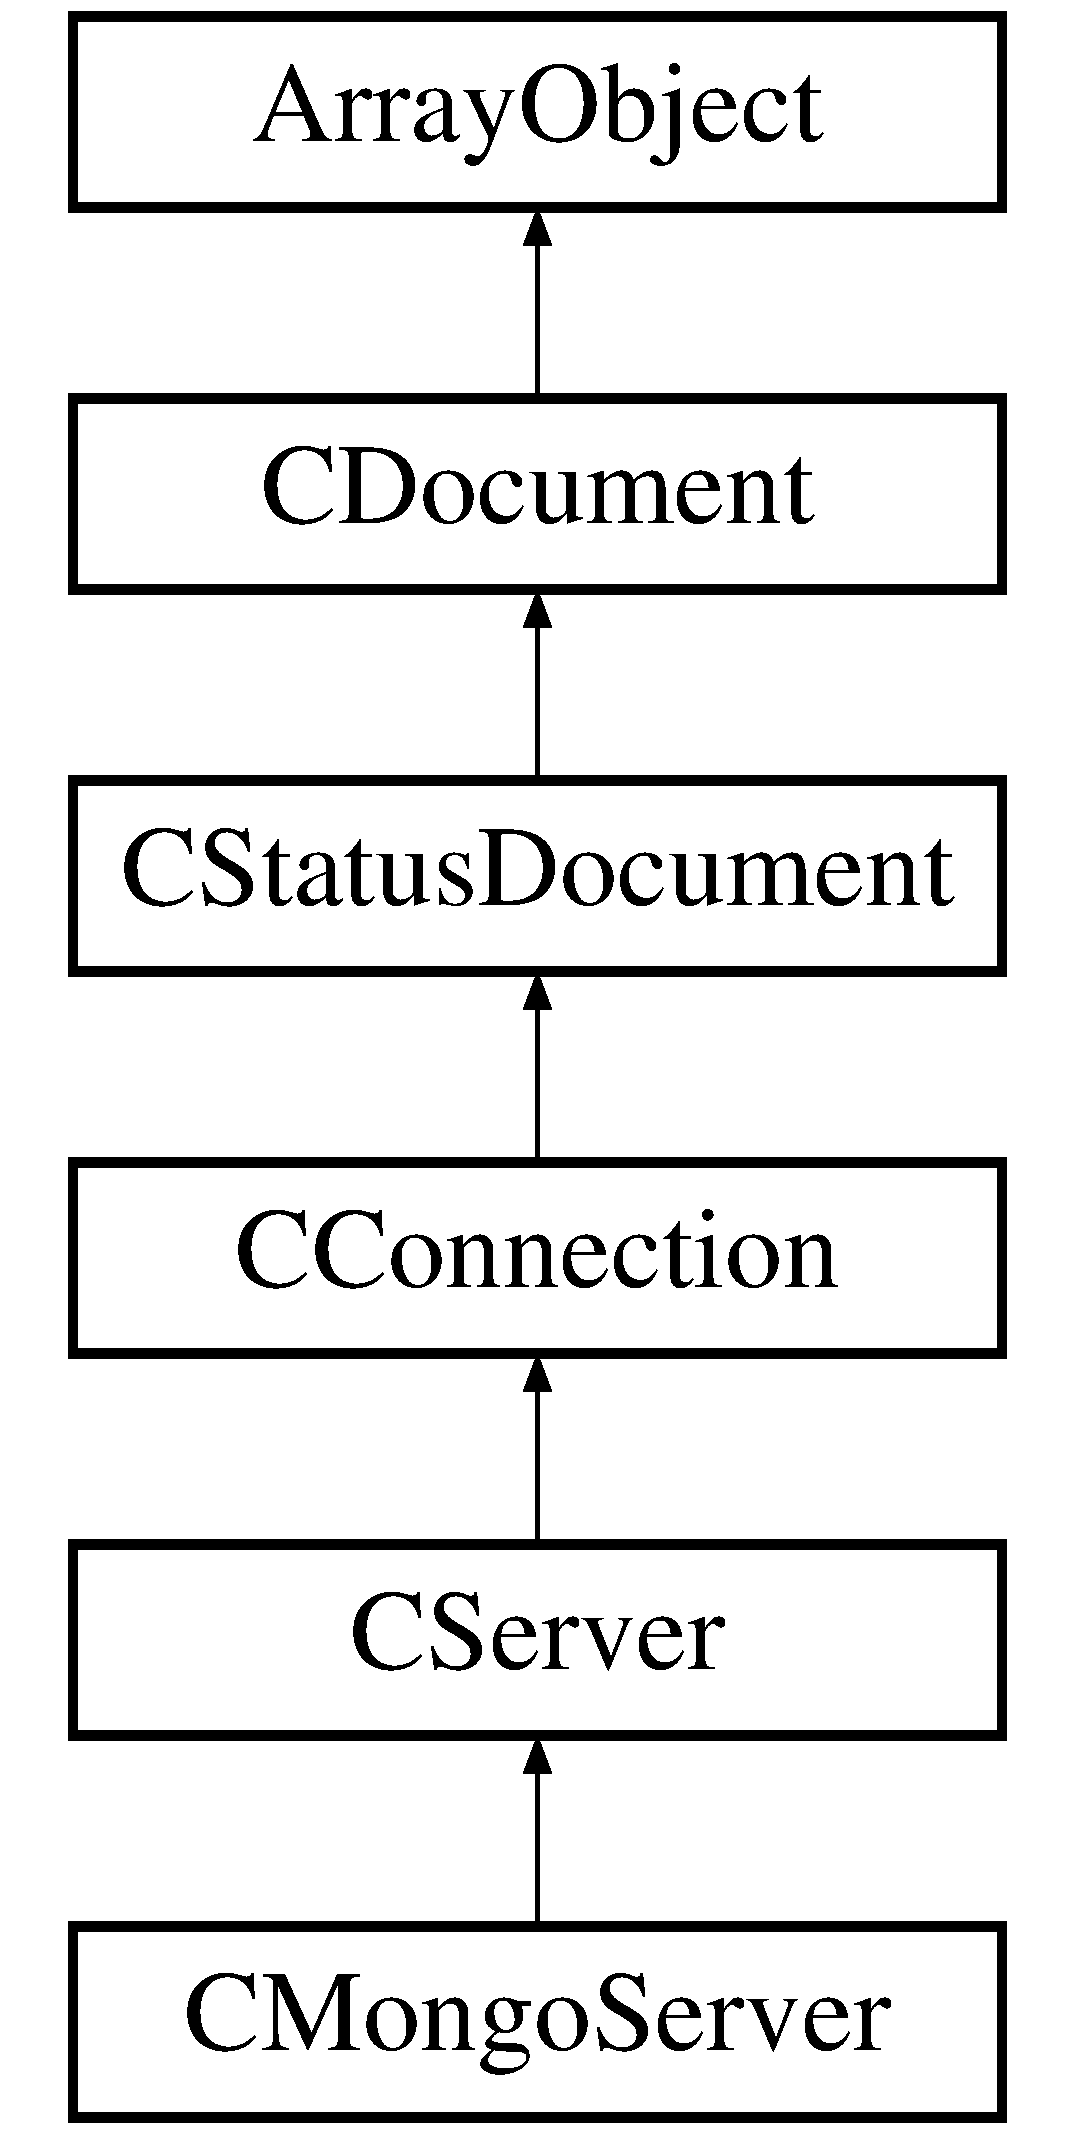
\includegraphics[height=6.000000cm]{class_c_mongo_server}
\end{center}
\end{figure}
\subsection*{Public Member Functions}
\begin{DoxyCompactItemize}
\item 
\hyperlink{class_c_mongo_server_ad70864e526dd380cc2440da5ff45ed50}{\-\_\-\-\_\-construct} (\$the\-Connection=N\-U\-L\-L, \$the\-Options=N\-U\-L\-L)
\item 
\hyperlink{class_c_mongo_server_a1842325257ca02c96123a1b49de976d0}{\-\_\-\-\_\-to\-String} ()
\item 
\hyperlink{class_c_mongo_server_a7bb403977a7f1a4d9a1391285f3ddd7e}{Connection} (\$the\-Value=N\-U\-L\-L, \$get\-Old=F\-A\-L\-S\-E)
\item 
\hyperlink{class_c_mongo_server_a68dce7b5cf2f8834d54495e290f64338}{Database} (\$the\-Database=N\-U\-L\-L)
\end{DoxyCompactItemize}
\subsection*{Additional Inherited Members}


\subsection{Constructor \& Destructor Documentation}
\hypertarget{class_c_mongo_server_ad70864e526dd380cc2440da5ff45ed50}{\index{C\-Mongo\-Server@{C\-Mongo\-Server}!\-\_\-\-\_\-construct@{\-\_\-\-\_\-construct}}
\index{\-\_\-\-\_\-construct@{\-\_\-\-\_\-construct}!CMongoServer@{C\-Mongo\-Server}}
\subsubsection[{\-\_\-\-\_\-construct}]{\setlength{\rightskip}{0pt plus 5cm}C\-Mongo\-Server\-::\-\_\-\-\_\-construct (
\begin{DoxyParamCaption}
\item[{}]{\$the\-Connection = {\ttfamily NULL}, }
\item[{}]{\$the\-Options = {\ttfamily NULL}}
\end{DoxyParamCaption}
)}}\label{class_c_mongo_server_ad70864e526dd380cc2440da5ff45ed50}
\subparagraph*{Instantiate class}

The method accepts the same parameters as the \hyperlink{}{Mongo} constructor, the first one represents the server U\-R\-L, the second represents the connection options.

The method will first attempt to instantiate the \hyperlink{}{Mongo} object, it will then store it in the connection data member.

If no parameter is provided, the method will assume the Mongo to connect to localhost on port 27017 and to initiate the connection.


\begin{DoxyParams}[1]{Parameters}
mixed & {\em \$the\-Connection} & Server U\-R\-L. \\
\hline
mixed & {\em \$the\-Options} & Connection options.\\
\hline
\end{DoxyParams}
public

\hyperlink{class_c_mongo_server_a7bb403977a7f1a4d9a1391285f3ddd7e}{Connection()} 

\subsection{Member Function Documentation}
\hypertarget{class_c_mongo_server_a1842325257ca02c96123a1b49de976d0}{\index{C\-Mongo\-Server@{C\-Mongo\-Server}!\-\_\-\-\_\-to\-String@{\-\_\-\-\_\-to\-String}}
\index{\-\_\-\-\_\-to\-String@{\-\_\-\-\_\-to\-String}!CMongoServer@{C\-Mongo\-Server}}
\subsubsection[{\-\_\-\-\_\-to\-String}]{\setlength{\rightskip}{0pt plus 5cm}C\-Mongo\-Server\-::\-\_\-\-\_\-to\-String (
\begin{DoxyParamCaption}
{}
\end{DoxyParamCaption}
)}}\label{class_c_mongo_server_a1842325257ca02c96123a1b49de976d0}
\subparagraph*{Return connection name}

In this class the method will return the server's connection U\-R\-L, which corresponds to the \hyperlink{}{k\-O\-F\-F\-S\-E\-T\-\_\-\-N\-A\-M\-E} offset.

public \begin{DoxyReturn}{Returns}
string The connection name. 
\end{DoxyReturn}
\hypertarget{class_c_mongo_server_a7bb403977a7f1a4d9a1391285f3ddd7e}{\index{C\-Mongo\-Server@{C\-Mongo\-Server}!Connection@{Connection}}
\index{Connection@{Connection}!CMongoServer@{C\-Mongo\-Server}}
\subsubsection[{Connection}]{\setlength{\rightskip}{0pt plus 5cm}C\-Mongo\-Server\-::\-Connection (
\begin{DoxyParamCaption}
\item[{}]{\$the\-Value = {\ttfamily NULL}, }
\item[{}]{\$get\-Old = {\ttfamily FALSE}}
\end{DoxyParamCaption}
)}}\label{class_c_mongo_server_a7bb403977a7f1a4d9a1391285f3ddd7e}
\subparagraph*{Manage native connection}

We overload this method to ensure the provided value is an instance of \hyperlink{}{Mongo}, if this is not the case, the method will raise an exception.

The method will attempt to parse the provided server U\-R\-L and store the results in the array part of the object. For more information on the parsed elements consult the P\-H\-P \hyperlink{}{parse\-\_\-url()} function.


\begin{DoxyParams}[1]{Parameters}
mixed & {\em \$the\-Value} & Native connection or operation. \\
\hline
boolean & {\em \$get\-Old} & {\ttfamily T\-R\-U\-E} get old value.\\
\hline
\end{DoxyParams}
public \begin{DoxyReturn}{Returns}
mixed {\itshape New} or {\itshape old} native connection.
\end{DoxyReturn}

\begin{DoxyExceptions}{Exceptions}
{\em Exception} & \\
\hline
\end{DoxyExceptions}
\hypertarget{class_c_mongo_server_a68dce7b5cf2f8834d54495e290f64338}{\index{C\-Mongo\-Server@{C\-Mongo\-Server}!Database@{Database}}
\index{Database@{Database}!CMongoServer@{C\-Mongo\-Server}}
\subsubsection[{Database}]{\setlength{\rightskip}{0pt plus 5cm}C\-Mongo\-Server\-::\-Database (
\begin{DoxyParamCaption}
\item[{}]{\$the\-Database = {\ttfamily NULL}}
\end{DoxyParamCaption}
)}}\label{class_c_mongo_server_a68dce7b5cf2f8834d54495e290f64338}
\subparagraph*{Generate a database object}

In this class we return \hyperlink{class_c_mongo_database}{C\-Mongo\-Database} instances, the provided parameter is interpreted as the database name.

If you omit the parameter, the method will raise an exception, in derived classes you can overload the method to provide a default database name.

If the object does not have its native connection, the method will also raise an exception.


\begin{DoxyParams}[1]{Parameters}
string & {\em \$the\-Database} & Database name.\\
\hline
\end{DoxyParams}
public \begin{DoxyReturn}{Returns}
mixed The database object.
\end{DoxyReturn}

\begin{DoxyExceptions}{Exceptions}
{\em Exception} & \hyperlink{class_c_status_document_a954dee06e219e0a0f2e7fa6edac56e28}{\-\_\-\-Is\-Inited()} \\
\hline
\end{DoxyExceptions}


The documentation for this class was generated from the following file\-:\begin{DoxyCompactItemize}
\item 
/\-Library/\-Web\-Server/\-Library/\-P\-H\-P\-Wrapper/classes/C\-Mongo\-Server.\-php\end{DoxyCompactItemize}

\hypertarget{class_c_neo4j_graph}{\section{C\-Neo4j\-Graph Class Reference}
\label{class_c_neo4j_graph}\index{C\-Neo4j\-Graph@{C\-Neo4j\-Graph}}
}
Inheritance diagram for C\-Neo4j\-Graph\-:\begin{figure}[H]
\begin{center}
\leavevmode
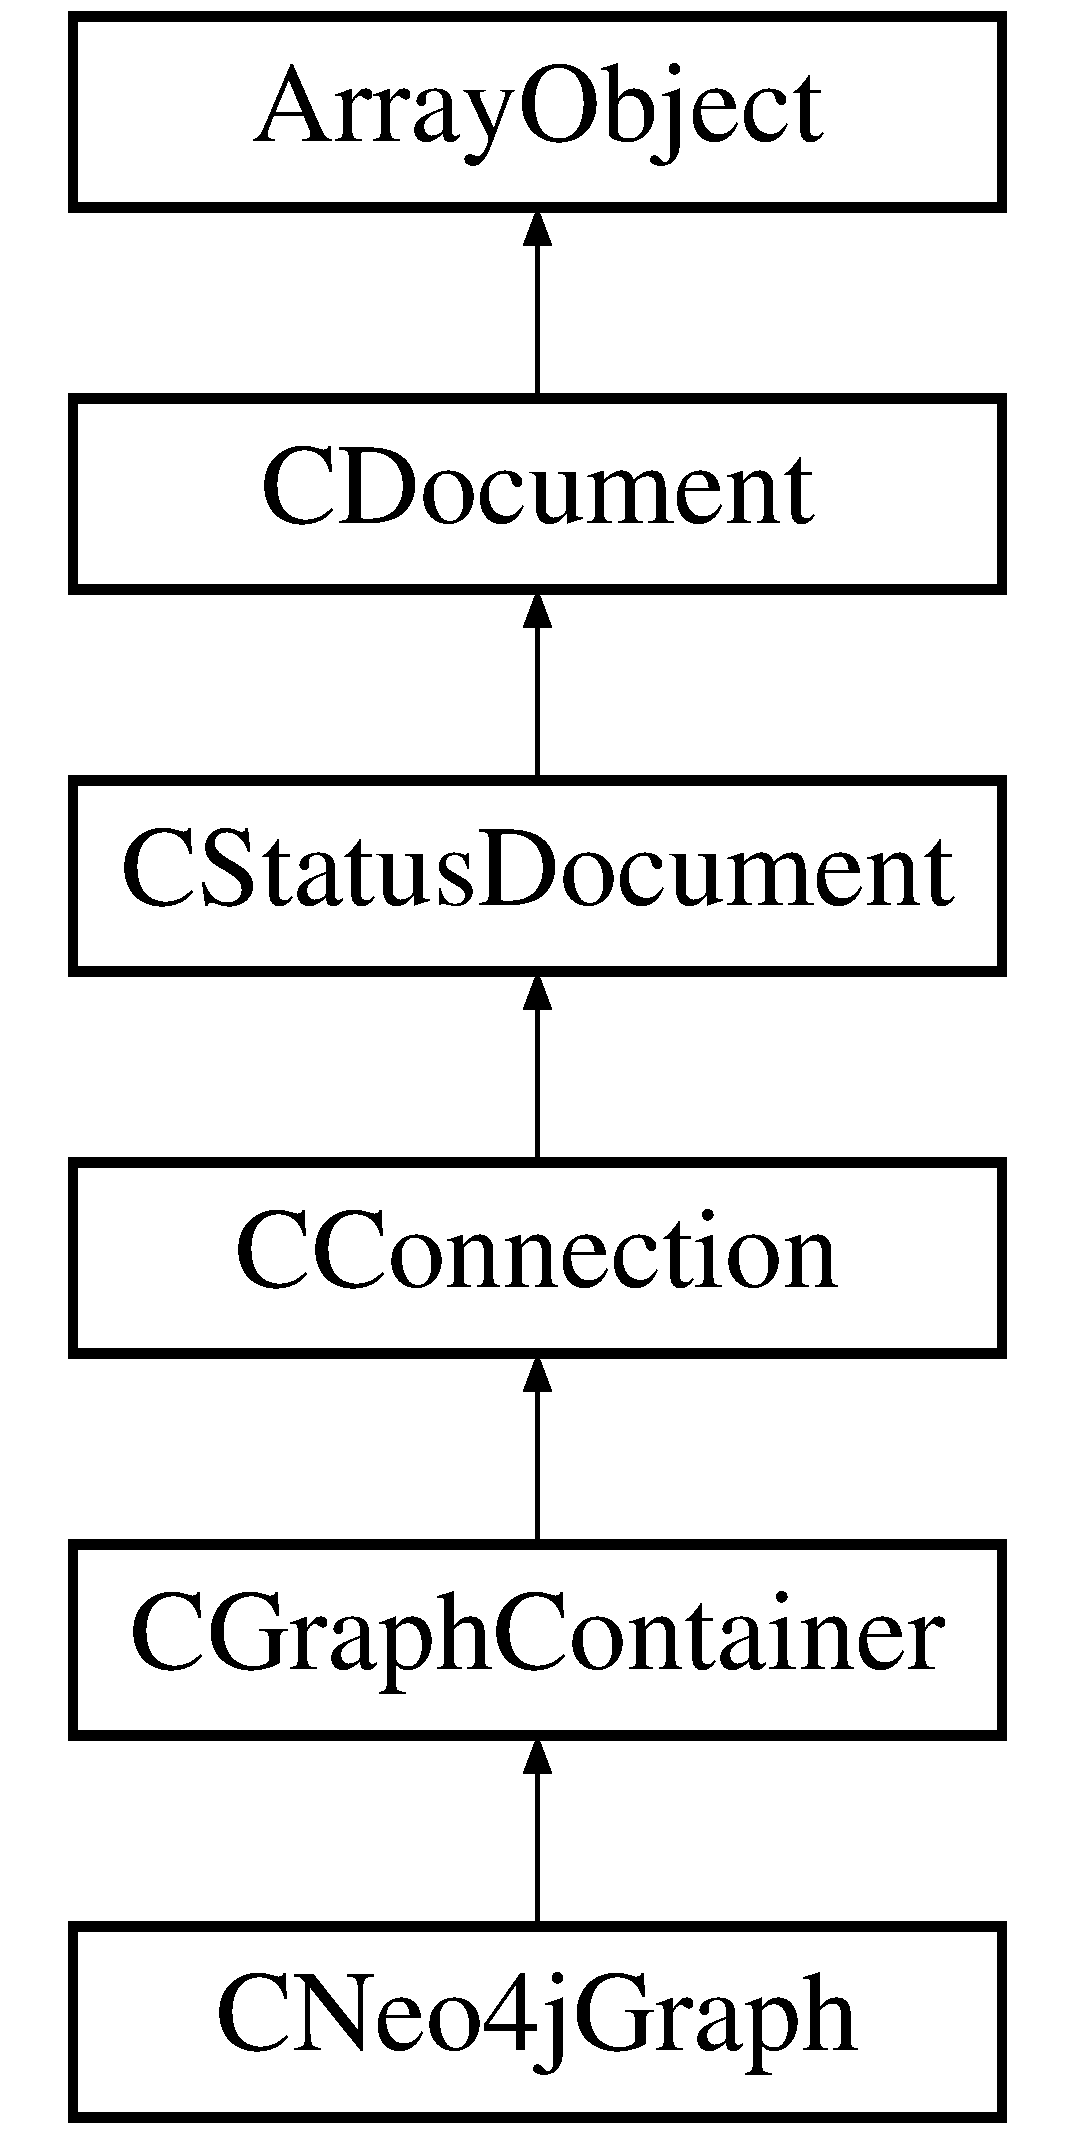
\includegraphics[height=6.000000cm]{class_c_neo4j_graph}
\end{center}
\end{figure}
\subsection*{Public Member Functions}
\begin{DoxyCompactItemize}
\item 
\hyperlink{class_c_neo4j_graph_ac73874c959201b5204020ab9f2df9ed8}{\-\_\-\-\_\-construct} (\$the\-Connection=N\-U\-L\-L, \$the\-Options=N\-U\-L\-L)
\item 
\hyperlink{class_c_neo4j_graph_a914022964c276ca0107345631e109382}{\-\_\-\-\_\-destruct} ()
\item 
\hyperlink{class_c_neo4j_graph_a6891f707fb08e36662d3d0c613f0da93}{\-\_\-\-\_\-to\-String} ()
\item 
\hyperlink{class_c_neo4j_graph_a651c716b812ce43b2590a5a7aa1f3efb}{Connection} (\$the\-Value=N\-U\-L\-L, \$get\-Old=F\-A\-L\-S\-E)
\item 
\hyperlink{class_c_neo4j_graph_a7da11906570d368e071fc7f858a751ca}{New\-Node} (\$the\-Properties=N\-U\-L\-L)
\item 
\hyperlink{class_c_neo4j_graph_a549a7280a0e5c181c21a68ffd49bd020}{Set\-Node} (\$the\-Node, \$the\-Properties=N\-U\-L\-L)
\item 
\hyperlink{class_c_neo4j_graph_ac42e2b030c642d9d04f3b5f0113fe9a2}{Get\-Node} (\$the\-Identifier, \$do\-Throw=F\-A\-L\-S\-E)
\item 
\hyperlink{class_c_neo4j_graph_a5833f27249ff962fb93ce840117172b0}{Del\-Node} (\$the\-Identifier)
\item 
\hyperlink{class_c_neo4j_graph_a9b9b2e18e4987c394406f5a086058757}{New\-Edge} (\$the\-Subject, \$the\-Predicate, \$the\-Object, \$the\-Properties=N\-U\-L\-L)
\item 
\hyperlink{class_c_neo4j_graph_a8688944572100526305443cd23f78a63}{Set\-Edge} (\$the\-Edge)
\item 
\hyperlink{class_c_neo4j_graph_a0352e11f4a5e856a09c19403c7a2e87b}{Get\-Edge} (\$the\-Identifier)
\item 
\hyperlink{class_c_neo4j_graph_a117ae458caca68a726f31ec9a5492ead}{Del\-Edge} (\$the\-Identifier)
\item 
\hyperlink{class_c_neo4j_graph_a2f999a5fff32d9b2317b4cf212abebff}{Get\-Node\-Properties} (\$the\-Node)
\item 
\hyperlink{class_c_neo4j_graph_a853373c66550ba67c2d1914f0aefbd33}{Get\-Node\-Edges} (\$the\-Node, \$the\-Predicate=N\-U\-L\-L, \$the\-Sense=N\-U\-L\-L)
\end{DoxyCompactItemize}
\subsection*{Additional Inherited Members}


\subsection{Constructor \& Destructor Documentation}
\hypertarget{class_c_neo4j_graph_ac73874c959201b5204020ab9f2df9ed8}{\index{C\-Neo4j\-Graph@{C\-Neo4j\-Graph}!\-\_\-\-\_\-construct@{\-\_\-\-\_\-construct}}
\index{\-\_\-\-\_\-construct@{\-\_\-\-\_\-construct}!CNeo4jGraph@{C\-Neo4j\-Graph}}
\subsubsection[{\-\_\-\-\_\-construct}]{\setlength{\rightskip}{0pt plus 5cm}C\-Neo4j\-Graph\-::\-\_\-\-\_\-construct (
\begin{DoxyParamCaption}
\item[{}]{\$the\-Connection = {\ttfamily NULL}, }
\item[{}]{\$the\-Options = {\ttfamily NULL}}
\end{DoxyParamCaption}
)}}\label{class_c_neo4j_graph_ac73874c959201b5204020ab9f2df9ed8}
\subparagraph*{Instantiate class}

You instantiate the class by providing a native connection, or the host and port. In the latter case the first parameter represents the host and the second the port.

If you do not provide any parameter the default \hyperlink{}{k\-G\-R\-A\-P\-H\-\_\-\-D\-E\-F\-\_\-\-H\-O\-S\-T} host and \hyperlink{}{k\-G\-R\-A\-P\-H\-\_\-\-D\-E\-F\-\_\-\-P\-O\-R\-T} port.


\begin{DoxyParams}[1]{Parameters}
mixed & {\em \$the\-Connection} & Native connection. \\
\hline
mixed & {\em \$the\-Options} & Connection options.\\
\hline
\end{DoxyParams}
public

\hyperlink{class_c_neo4j_graph_a651c716b812ce43b2590a5a7aa1f3efb}{Connection()} \hypertarget{class_c_neo4j_graph_a914022964c276ca0107345631e109382}{\index{C\-Neo4j\-Graph@{C\-Neo4j\-Graph}!\-\_\-\-\_\-destruct@{\-\_\-\-\_\-destruct}}
\index{\-\_\-\-\_\-destruct@{\-\_\-\-\_\-destruct}!CNeo4jGraph@{C\-Neo4j\-Graph}}
\subsubsection[{\-\_\-\-\_\-destruct}]{\setlength{\rightskip}{0pt plus 5cm}C\-Neo4j\-Graph\-::\-\_\-\-\_\-destruct (
\begin{DoxyParamCaption}
{}
\end{DoxyParamCaption}
)}}\label{class_c_neo4j_graph_a914022964c276ca0107345631e109382}
\subparagraph*{Destructor}

We implement the destructor to get rid of the graph\-: the Neo4j P\-H\-P interface, for instance, has closures that cannot be serialised, so we need to reset the graph \hyperlink{class_c_neo4j_graph_a651c716b812ce43b2590a5a7aa1f3efb}{Connection()} before destroying the object.

public 

\subsection{Member Function Documentation}
\hypertarget{class_c_neo4j_graph_a6891f707fb08e36662d3d0c613f0da93}{\index{C\-Neo4j\-Graph@{C\-Neo4j\-Graph}!\-\_\-\-\_\-to\-String@{\-\_\-\-\_\-to\-String}}
\index{\-\_\-\-\_\-to\-String@{\-\_\-\-\_\-to\-String}!CNeo4jGraph@{C\-Neo4j\-Graph}}
\subsubsection[{\-\_\-\-\_\-to\-String}]{\setlength{\rightskip}{0pt plus 5cm}C\-Neo4j\-Graph\-::\-\_\-\-\_\-to\-String (
\begin{DoxyParamCaption}
{}
\end{DoxyParamCaption}
)}}\label{class_c_neo4j_graph_a6891f707fb08e36662d3d0c613f0da93}
\subparagraph*{Return connection name}

This method should return the current connection's name.

In this class we return the host and port names.

public \begin{DoxyReturn}{Returns}
string The connection name. 
\end{DoxyReturn}
\hypertarget{class_c_neo4j_graph_a651c716b812ce43b2590a5a7aa1f3efb}{\index{C\-Neo4j\-Graph@{C\-Neo4j\-Graph}!Connection@{Connection}}
\index{Connection@{Connection}!CNeo4jGraph@{C\-Neo4j\-Graph}}
\subsubsection[{Connection}]{\setlength{\rightskip}{0pt plus 5cm}C\-Neo4j\-Graph\-::\-Connection (
\begin{DoxyParamCaption}
\item[{}]{\$the\-Value = {\ttfamily NULL}, }
\item[{}]{\$get\-Old = {\ttfamily FALSE}}
\end{DoxyParamCaption}
)}}\label{class_c_neo4j_graph_a651c716b812ce43b2590a5a7aa1f3efb}
\subparagraph*{Manage native connection}

We overload this method to ensure that the provided container is a Neo4j client.


\begin{DoxyParams}[1]{Parameters}
mixed & {\em \$the\-Value} & Persistent container or operation. \\
\hline
boolean & {\em \$get\-Old} & {\ttfamily T\-R\-U\-E} get old value.\\
\hline
\end{DoxyParams}
public \begin{DoxyReturn}{Returns}
mixed {\itshape New} or {\itshape old} native container.
\end{DoxyReturn}

\begin{DoxyExceptions}{Exceptions}
{\em Exception} & \\
\hline
\end{DoxyExceptions}
\hypertarget{class_c_neo4j_graph_a117ae458caca68a726f31ec9a5492ead}{\index{C\-Neo4j\-Graph@{C\-Neo4j\-Graph}!Del\-Edge@{Del\-Edge}}
\index{Del\-Edge@{Del\-Edge}!CNeo4jGraph@{C\-Neo4j\-Graph}}
\subsubsection[{Del\-Edge}]{\setlength{\rightskip}{0pt plus 5cm}C\-Neo4j\-Graph\-::\-Del\-Edge (
\begin{DoxyParamCaption}
\item[{}]{\$the\-Identifier}
\end{DoxyParamCaption}
)}}\label{class_c_neo4j_graph_a117ae458caca68a726f31ec9a5492ead}
\subparagraph*{Delete an existing edge}

This method should delete the provided edge from the current graph.

The method should return {\ttfamily T\-R\-U\-E} if the operation was successful and {\ttfamily N\-U\-L\-L} if the provided identifier is not resolved.


\begin{DoxyParams}[1]{Parameters}
mixed & {\em \$the\-Identifier} & Edge identifier.\\
\hline
\end{DoxyParams}
public \begin{DoxyReturn}{Returns}
mixed 
\end{DoxyReturn}
\hypertarget{class_c_neo4j_graph_a5833f27249ff962fb93ce840117172b0}{\index{C\-Neo4j\-Graph@{C\-Neo4j\-Graph}!Del\-Node@{Del\-Node}}
\index{Del\-Node@{Del\-Node}!CNeo4jGraph@{C\-Neo4j\-Graph}}
\subsubsection[{Del\-Node}]{\setlength{\rightskip}{0pt plus 5cm}C\-Neo4j\-Graph\-::\-Del\-Node (
\begin{DoxyParamCaption}
\item[{}]{\$the\-Identifier}
\end{DoxyParamCaption}
)}}\label{class_c_neo4j_graph_a5833f27249ff962fb93ce840117172b0}
\subparagraph*{Delete an existing node}

In this class we accept either the actual node, or the node identifier.


\begin{DoxyParams}[1]{Parameters}
mixed & {\em \$the\-Identifier} & Node identifier.\\
\hline
\end{DoxyParams}
public \begin{DoxyReturn}{Returns}
mixed 
\end{DoxyReturn}
\hypertarget{class_c_neo4j_graph_a0352e11f4a5e856a09c19403c7a2e87b}{\index{C\-Neo4j\-Graph@{C\-Neo4j\-Graph}!Get\-Edge@{Get\-Edge}}
\index{Get\-Edge@{Get\-Edge}!CNeo4jGraph@{C\-Neo4j\-Graph}}
\subsubsection[{Get\-Edge}]{\setlength{\rightskip}{0pt plus 5cm}C\-Neo4j\-Graph\-::\-Get\-Edge (
\begin{DoxyParamCaption}
\item[{}]{\$the\-Identifier}
\end{DoxyParamCaption}
)}}\label{class_c_neo4j_graph_a0352e11f4a5e856a09c19403c7a2e87b}
\subparagraph*{Get an existing edge}

In this class we return the edge corresponding to the provided I\-D, or {\ttfamily N\-U\-L\-L}.


\begin{DoxyParams}[1]{Parameters}
mixed & {\em \$the\-Identifier} & Edge identifier.\\
\hline
\end{DoxyParams}
public \begin{DoxyReturn}{Returns}
mixed 
\end{DoxyReturn}
\hypertarget{class_c_neo4j_graph_ac42e2b030c642d9d04f3b5f0113fe9a2}{\index{C\-Neo4j\-Graph@{C\-Neo4j\-Graph}!Get\-Node@{Get\-Node}}
\index{Get\-Node@{Get\-Node}!CNeo4jGraph@{C\-Neo4j\-Graph}}
\subsubsection[{Get\-Node}]{\setlength{\rightskip}{0pt plus 5cm}C\-Neo4j\-Graph\-::\-Get\-Node (
\begin{DoxyParamCaption}
\item[{}]{\$the\-Identifier, }
\item[{}]{\$do\-Throw = {\ttfamily FALSE}}
\end{DoxyParamCaption}
)}}\label{class_c_neo4j_graph_ac42e2b030c642d9d04f3b5f0113fe9a2}
\subparagraph*{Get an existing node}

In this class we return the node corresponding to the provided identifier or {\ttfamily N\-U\-L\-L}.

If the provided identifier is not an integer, we raise an exception.


\begin{DoxyParams}[1]{Parameters}
mixed & {\em \$the\-Identifier} & Node identifier. \\
\hline
boolean & {\em \$do\-Throw} & T\-R\-U\-E throw exception if not found.\\
\hline
\end{DoxyParams}
public \begin{DoxyReturn}{Returns}
mixed 
\end{DoxyReturn}
\hypertarget{class_c_neo4j_graph_a853373c66550ba67c2d1914f0aefbd33}{\index{C\-Neo4j\-Graph@{C\-Neo4j\-Graph}!Get\-Node\-Edges@{Get\-Node\-Edges}}
\index{Get\-Node\-Edges@{Get\-Node\-Edges}!CNeo4jGraph@{C\-Neo4j\-Graph}}
\subsubsection[{Get\-Node\-Edges}]{\setlength{\rightskip}{0pt plus 5cm}C\-Neo4j\-Graph\-::\-Get\-Node\-Edges (
\begin{DoxyParamCaption}
\item[{}]{\$the\-Node, }
\item[{}]{\$the\-Predicate = {\ttfamily NULL}, }
\item[{}]{\$the\-Sense = {\ttfamily NULL}}
\end{DoxyParamCaption}
)}}\label{class_c_neo4j_graph_a853373c66550ba67c2d1914f0aefbd33}
\subparagraph*{Get node edges}

In this class we accept the following values\-:


\begin{DoxyItemize}
\item {\ttfamily \$the\-Node}\-: Either the node identifier or the node object. 
\item {\ttfamily \$the\-Predicate}\-: Either a predicate or a predicates list, the elements can be of any type, provided they can be cast to a string. 
\item {\ttfamily \$the\-Sense}\-: If this parameter is omitted, we set \hyperlink{}{k\-T\-Y\-P\-E\-\_\-\-R\-E\-L\-A\-T\-I\-O\-N\-\_\-\-A\-L\-L} as default. 
\end{DoxyItemize}


\begin{DoxyParams}[1]{Parameters}
mixed & {\em \$the\-Node} & Reference node. \\
\hline
mixed & {\em \$the\-Predicate} & Edge predicates filter. \\
\hline
string & {\em \$the\-Sense} & Relationship sense.\\
\hline
\end{DoxyParams}
public \begin{DoxyReturn}{Returns}
mixed 
\end{DoxyReturn}
\hypertarget{class_c_neo4j_graph_a2f999a5fff32d9b2317b4cf212abebff}{\index{C\-Neo4j\-Graph@{C\-Neo4j\-Graph}!Get\-Node\-Properties@{Get\-Node\-Properties}}
\index{Get\-Node\-Properties@{Get\-Node\-Properties}!CNeo4jGraph@{C\-Neo4j\-Graph}}
\subsubsection[{Get\-Node\-Properties}]{\setlength{\rightskip}{0pt plus 5cm}C\-Neo4j\-Graph\-::\-Get\-Node\-Properties (
\begin{DoxyParamCaption}
\item[{}]{\$the\-Node}
\end{DoxyParamCaption}
)}}\label{class_c_neo4j_graph_a2f999a5fff32d9b2317b4cf212abebff}
\subparagraph*{Get node properties}

In this class we check whether the node is a Neo4j graph node or an integer, in all other cases we raise an exception.


\begin{DoxyParams}[1]{Parameters}
mixed & {\em \$the\-Node} & Node object or reference.\\
\hline
\end{DoxyParams}
public \begin{DoxyReturn}{Returns}
array The node properties 
\end{DoxyReturn}
\hypertarget{class_c_neo4j_graph_a9b9b2e18e4987c394406f5a086058757}{\index{C\-Neo4j\-Graph@{C\-Neo4j\-Graph}!New\-Edge@{New\-Edge}}
\index{New\-Edge@{New\-Edge}!CNeo4jGraph@{C\-Neo4j\-Graph}}
\subsubsection[{New\-Edge}]{\setlength{\rightskip}{0pt plus 5cm}C\-Neo4j\-Graph\-::\-New\-Edge (
\begin{DoxyParamCaption}
\item[{}]{\$the\-Subject, }
\item[{}]{\$the\-Predicate, }
\item[{}]{\$the\-Object, }
\item[{}]{\$the\-Properties = {\ttfamily NULL}}
\end{DoxyParamCaption}
)}}\label{class_c_neo4j_graph_a9b9b2e18e4987c394406f5a086058757}
\subparagraph*{Create a new edge}

In this class we instantiate the relationship and set the subject and object nodes, we finally convert the provided predicate to a string.

Both the subject and object nodes can be provided either as a node object or as a node identifier, the method will take care of fetching the referenced nodes. If any node is neither a node object or identifier, or if the referenced node cannot be found, the method will raise an exception.


\begin{DoxyParams}[1]{Parameters}
mixed & {\em \$the\-Subject} & Subject node. \\
\hline
array & {\em \$the\-Predicate} & Edge predicate. \\
\hline
mixed & {\em \$the\-Object} & Object node. \\
\hline
array & {\em \$the\-Properties} & Edge properties.\\
\hline
\end{DoxyParams}
public \begin{DoxyReturn}{Returns}
mixed 
\end{DoxyReturn}
\hypertarget{class_c_neo4j_graph_a7da11906570d368e071fc7f858a751ca}{\index{C\-Neo4j\-Graph@{C\-Neo4j\-Graph}!New\-Node@{New\-Node}}
\index{New\-Node@{New\-Node}!CNeo4jGraph@{C\-Neo4j\-Graph}}
\subsubsection[{New\-Node}]{\setlength{\rightskip}{0pt plus 5cm}C\-Neo4j\-Graph\-::\-New\-Node (
\begin{DoxyParamCaption}
\item[{}]{\$the\-Properties = {\ttfamily NULL}}
\end{DoxyParamCaption}
)}}\label{class_c_neo4j_graph_a7da11906570d368e071fc7f858a751ca}
\subparagraph*{Create a new node}

In this class we return a new Neo4j Node instance.


\begin{DoxyParams}[1]{Parameters}
array & {\em \$the\-Properties} & Node properties.\\
\hline
\end{DoxyParams}
public \begin{DoxyReturn}{Returns}
mixed 
\end{DoxyReturn}
\hypertarget{class_c_neo4j_graph_a8688944572100526305443cd23f78a63}{\index{C\-Neo4j\-Graph@{C\-Neo4j\-Graph}!Set\-Edge@{Set\-Edge}}
\index{Set\-Edge@{Set\-Edge}!CNeo4jGraph@{C\-Neo4j\-Graph}}
\subsubsection[{Set\-Edge}]{\setlength{\rightskip}{0pt plus 5cm}C\-Neo4j\-Graph\-::\-Set\-Edge (
\begin{DoxyParamCaption}
\item[{}]{\$the\-Edge}
\end{DoxyParamCaption}
)}}\label{class_c_neo4j_graph_a8688944572100526305443cd23f78a63}
\subparagraph*{Save an edge}

In this class we save the provided edge.


\begin{DoxyParams}[1]{Parameters}
mixed & {\em \$the\-Edge} & Edge to be saved.\\
\hline
\end{DoxyParams}
public \begin{DoxyReturn}{Returns}
mixed 
\end{DoxyReturn}
\hypertarget{class_c_neo4j_graph_a549a7280a0e5c181c21a68ffd49bd020}{\index{C\-Neo4j\-Graph@{C\-Neo4j\-Graph}!Set\-Node@{Set\-Node}}
\index{Set\-Node@{Set\-Node}!CNeo4jGraph@{C\-Neo4j\-Graph}}
\subsubsection[{Set\-Node}]{\setlength{\rightskip}{0pt plus 5cm}C\-Neo4j\-Graph\-::\-Set\-Node (
\begin{DoxyParamCaption}
\item[{}]{\$the\-Node, }
\item[{}]{\$the\-Properties = {\ttfamily NULL}}
\end{DoxyParamCaption}
)}}\label{class_c_neo4j_graph_a549a7280a0e5c181c21a68ffd49bd020}
\subparagraph*{Save a node}

In this class we check if the provided node is of the correct type, save it and return its identifier.

If provided, the second parameter must be an array or Array\-Object, or the method will raise an exception.


\begin{DoxyParams}[1]{Parameters}
mixed & {\em \$the\-Node} & Node to be saved. \\
\hline
mixed & {\em \$the\-Properties} & Node properties.\\
\hline
\end{DoxyParams}
public \begin{DoxyReturn}{Returns}
mixed 
\end{DoxyReturn}


The documentation for this class was generated from the following file\-:\begin{DoxyCompactItemize}
\item 
/\-Library/\-Web\-Server/\-Library/\-P\-H\-P\-Wrapper/classes/C\-Neo4j\-Graph.\-php\end{DoxyCompactItemize}

\hypertarget{class_c_node}{\section{C\-Node Class Reference}
\label{class_c_node}\index{C\-Node@{C\-Node}}
}
Inheritance diagram for C\-Node\-:\begin{figure}[H]
\begin{center}
\leavevmode
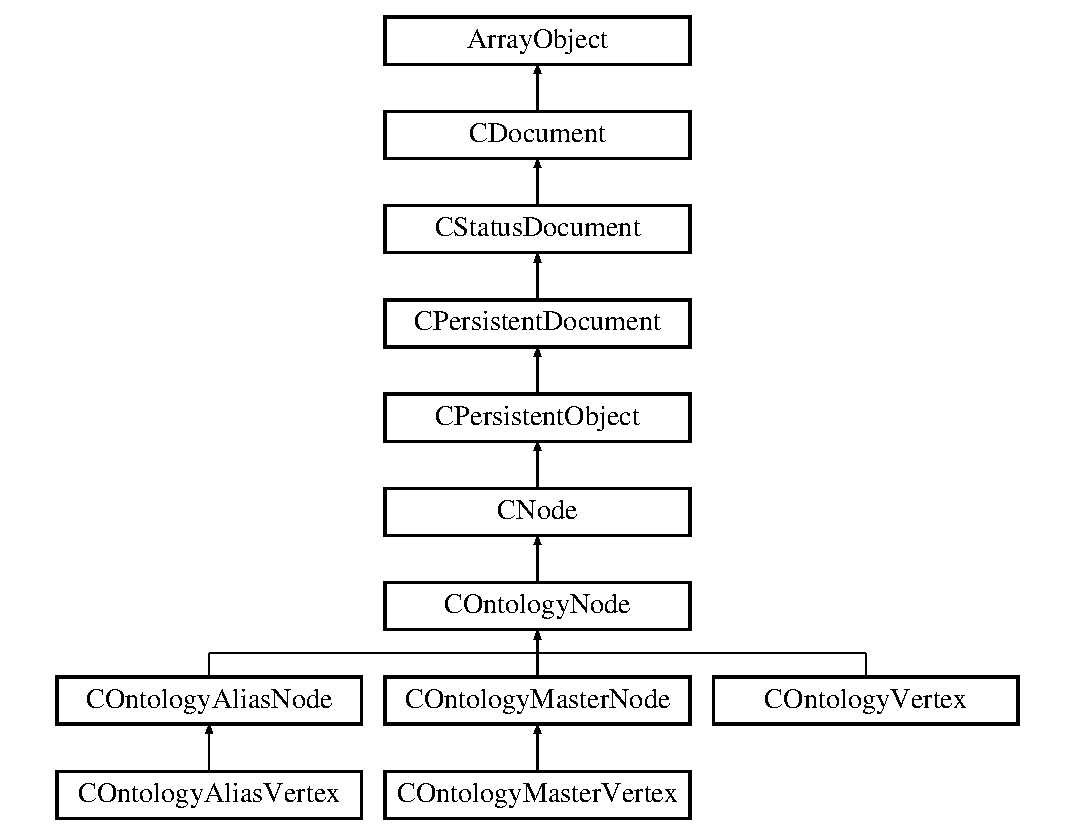
\includegraphics[height=9.000000cm]{class_c_node}
\end{center}
\end{figure}
\subsection*{Public Member Functions}
\begin{DoxyCompactItemize}
\item 
\hyperlink{class_c_node_adf7a1752d6bc7cd6d5cbc8f11d75c3f9}{\-\_\-\-\_\-to\-String} ()
\item 
\hyperlink{class_c_node_a3d2db41c8c96b7ac2d08ce7d2a36d4ea}{P\-I\-D} (\$the\-Value=N\-U\-L\-L, \$get\-Old=F\-A\-L\-S\-E)
\item 
\hyperlink{class_c_node_a885e13767f6df4c17ca2757b83f0d508}{Term} (\$the\-Value=N\-U\-L\-L, \$get\-Old=F\-A\-L\-S\-E)
\item 
\hyperlink{class_c_node_a5c1d1ac1bc2729951de092abaca3244f}{Description} (\$the\-Language=N\-U\-L\-L, \$the\-Value=N\-U\-L\-L, \$get\-Old=F\-A\-L\-S\-E)
\item 
\hyperlink{class_c_node_a864f2abf26ebac8a6a17ccf44d073f48}{Synonym} (\$the\-Value=N\-U\-L\-L, \$the\-Operation=N\-U\-L\-L, \$get\-Old=F\-A\-L\-S\-E)
\item 
\hyperlink{class_c_node_af2b8ddaa93259dac31fc34e4b70ef8ed}{Relate\-To} (\$the\-Predicate, \$the\-Object, \$the\-Connection=N\-U\-L\-L, \$do\-Propagate=T\-R\-U\-E)
\end{DoxyCompactItemize}
\subsection*{Protected Member Functions}
\begin{DoxyCompactItemize}
\item 
\hyperlink{class_c_node_aa888912a5e5303c88e8576d062b942d6}{\-\_\-\-Preset} (\&\$the\-Offset, \&\$the\-Value)
\item 
\hyperlink{class_c_node_affdb1c5688a438b055c90c60be4fe739}{\-\_\-\-Preunset} (\&\$the\-Offset)
\item 
\hyperlink{class_c_node_ac7ce04dd9d8c98638adbbb13a5909986}{\-\_\-\-New\-Edge} ()
\item 
\hyperlink{class_c_node_afb22b2eec5a60d6e417e358b5a2ad5ef}{\-\_\-\-Ready} ()
\end{DoxyCompactItemize}
\subsection*{Additional Inherited Members}


\subsection{Member Function Documentation}
\hypertarget{class_c_node_adf7a1752d6bc7cd6d5cbc8f11d75c3f9}{\index{C\-Node@{C\-Node}!\-\_\-\-\_\-to\-String@{\-\_\-\-\_\-to\-String}}
\index{\-\_\-\-\_\-to\-String@{\-\_\-\-\_\-to\-String}!CNode@{C\-Node}}
\subsubsection[{\-\_\-\-\_\-to\-String}]{\setlength{\rightskip}{0pt plus 5cm}C\-Node\-::\-\_\-\-\_\-to\-String (
\begin{DoxyParamCaption}
{}
\end{DoxyParamCaption}
)}}\label{class_c_node_adf7a1752d6bc7cd6d5cbc8f11d75c3f9}
\subparagraph*{Return object name}

This method should return the current object's name which should represent the unique identifier of the object.

By default we return the string representation of the term, \hyperlink{}{k\-T\-A\-G\-\_\-\-T\-E\-R\-M}.

public \begin{DoxyReturn}{Returns}
string The connection name. 
\end{DoxyReturn}
\hypertarget{class_c_node_ac7ce04dd9d8c98638adbbb13a5909986}{\index{C\-Node@{C\-Node}!\-\_\-\-New\-Edge@{\-\_\-\-New\-Edge}}
\index{\-\_\-\-New\-Edge@{\-\_\-\-New\-Edge}!CNode@{C\-Node}}
\subsubsection[{\-\_\-\-New\-Edge}]{\setlength{\rightskip}{0pt plus 5cm}C\-Node\-::\-\_\-\-New\-Edge (
\begin{DoxyParamCaption}
{}
\end{DoxyParamCaption}
)\hspace{0.3cm}{\ttfamily [protected]}}}\label{class_c_node_ac7ce04dd9d8c98638adbbb13a5909986}
\subparagraph*{Return a new edge instance}

This method should return a new edge instance, its goal is to instantiate the correct edge type.

In this class we return a \hyperlink{class_c_edge}{C\-Edge} instance.

protected \begin{DoxyReturn}{Returns}
\hyperlink{class_c_edge}{C\-Edge} 
\end{DoxyReturn}
\hypertarget{class_c_node_aa888912a5e5303c88e8576d062b942d6}{\index{C\-Node@{C\-Node}!\-\_\-\-Preset@{\-\_\-\-Preset}}
\index{\-\_\-\-Preset@{\-\_\-\-Preset}!CNode@{C\-Node}}
\subsubsection[{\-\_\-\-Preset}]{\setlength{\rightskip}{0pt plus 5cm}C\-Node\-::\-\_\-\-Preset (
\begin{DoxyParamCaption}
\item[{\&}]{\$the\-Offset, }
\item[{\&}]{\$the\-Value}
\end{DoxyParamCaption}
)\hspace{0.3cm}{\ttfamily [protected]}}}\label{class_c_node_aa888912a5e5303c88e8576d062b942d6}
\subparagraph*{Handle offset before setting it}

In this class we ensure that the \hyperlink{}{k\-T\-A\-G\-\_\-\-K\-I\-N\-D} and \hyperlink{}{k\-T\-A\-G\-\_\-\-D\-E\-S\-C\-R\-I\-P\-T\-I\-O\-N} offsets are an arrays, Array\-Object instances are not counted as an array.

We also ensure that the persistent identifier, \hyperlink{}{k\-T\-A\-G\-\_\-\-P\-I\-D}, is not modified if the object is committed.


\begin{DoxyParams}[1]{Parameters}
reference & {\em \&\$the\-Offset} & Offset. \\
\hline
reference & {\em \&\$the\-Value} & Value to set at offset.\\
\hline
\end{DoxyParams}
protected


\begin{DoxyExceptions}{Exceptions}
{\em Exception} & \\
\hline
\end{DoxyExceptions}
\begin{DoxySeeAlso}{See Also}
k\-T\-A\-G\-\_\-\-K\-I\-N\-D 
\end{DoxySeeAlso}
\hypertarget{class_c_node_affdb1c5688a438b055c90c60be4fe739}{\index{C\-Node@{C\-Node}!\-\_\-\-Preunset@{\-\_\-\-Preunset}}
\index{\-\_\-\-Preunset@{\-\_\-\-Preunset}!CNode@{C\-Node}}
\subsubsection[{\-\_\-\-Preunset}]{\setlength{\rightskip}{0pt plus 5cm}C\-Node\-::\-\_\-\-Preunset (
\begin{DoxyParamCaption}
\item[{\&}]{\$the\-Offset}
\end{DoxyParamCaption}
)\hspace{0.3cm}{\ttfamily [protected]}}}\label{class_c_node_affdb1c5688a438b055c90c60be4fe739}
\subparagraph*{Handle offset before unsetting it}

In this class we prevent the modification of persistent attributes, in this class\-: \hyperlink{}{k\-T\-A\-G\-\_\-\-P\-I\-D}.


\begin{DoxyParams}[1]{Parameters}
reference & {\em \&\$the\-Offset} & Offset.\\
\hline
\end{DoxyParams}
protected


\begin{DoxyExceptions}{Exceptions}
{\em Exception} & \hyperlink{class_c_status_document_ab7d96fd4588cf7d5432fc65a1d1fb076}{\-\_\-\-Is\-Committed()}\\
\hline
\end{DoxyExceptions}
\begin{DoxySeeAlso}{See Also}
k\-T\-A\-G\-\_\-\-P\-I\-D 
\end{DoxySeeAlso}
\hypertarget{class_c_node_afb22b2eec5a60d6e417e358b5a2ad5ef}{\index{C\-Node@{C\-Node}!\-\_\-\-Ready@{\-\_\-\-Ready}}
\index{\-\_\-\-Ready@{\-\_\-\-Ready}!CNode@{C\-Node}}
\subsubsection[{\-\_\-\-Ready}]{\setlength{\rightskip}{0pt plus 5cm}C\-Node\-::\-\_\-\-Ready (
\begin{DoxyParamCaption}
{}
\end{DoxyParamCaption}
)\hspace{0.3cm}{\ttfamily [protected]}}}\label{class_c_node_afb22b2eec5a60d6e417e358b5a2ad5ef}
\subparagraph*{Determine if the object is ready}

In this class we tie the \hyperlink{class_c_status_document_a954dee06e219e0a0f2e7fa6edac56e28}{\-\_\-\-Is\-Inited()} status to the presence or absence of the \hyperlink{}{k\-T\-A\-G\-\_\-\-T\-E\-R\-M} offset.

protected \begin{DoxyReturn}{Returns}
boolean {\ttfamily T\-R\-U\-E} means \hyperlink{}{.  \-\_\-\-Ready()  k\-T\-A\-G\-\_\-\-T\-E\-R\-M }
\end{DoxyReturn}
\hypertarget{class_c_node_a5c1d1ac1bc2729951de092abaca3244f}{\index{C\-Node@{C\-Node}!Description@{Description}}
\index{Description@{Description}!CNode@{C\-Node}}
\subsubsection[{Description}]{\setlength{\rightskip}{0pt plus 5cm}C\-Node\-::\-Description (
\begin{DoxyParamCaption}
\item[{}]{\$the\-Language = {\ttfamily NULL}, }
\item[{}]{\$the\-Value = {\ttfamily NULL}, }
\item[{}]{\$get\-Old = {\ttfamily FALSE}}
\end{DoxyParamCaption}
)}}\label{class_c_node_a5c1d1ac1bc2729951de092abaca3244f}
\subparagraph*{Manage node description}

The node {\itshape description}, \hyperlink{}{k\-T\-A\-G\-\_\-\-D\-E\-S\-C\-R\-I\-P\-T\-I\-O\-N}, represents the node's long label or extended definition. It is an optional attribute of the object that holds an array of elements in which the index is represented by the language code and the value is the string.

No two elements may share the same language code.

The description depends on the context in which the object is, as opposed as the definition which does not depend on the context.

The method accepts the following parameters\-:


\begin{DoxyItemize}
\item {\ttfamily \$the\-Language}\-: Language code. 
\item {\ttfamily \$the\-Value}\-: The description string or the operation, depending on its value\-: 
\begin{DoxyItemize}
\item {\ttfamily N\-U\-L\-L}\-: Return the string corresponding to the provided language. 
\item {\ttfamily F\-A\-L\-S\-E}\-: Delete the element corresponding to the provided language. 
\item {\itshape other}\-: Any other value represents the description string that will be set or replace the entry for the provided language. 
\end{DoxyItemize}
\item {\ttfamily \$get\-Old}\-: If {\ttfamily T\-R\-U\-E}, the method will return the description string {\itshape before} it was eventually modified; if {\ttfamily F\-A\-L\-S\-E}, the method will return the value {\itshape after} eventual modifications. 
\end{DoxyItemize}


\begin{DoxyParams}[1]{Parameters}
mixed & {\em \$the\-Language} & Language code. \\
\hline
mixed & {\em \$the\-Value} & Description or operation. \\
\hline
boolean & {\em \$get\-Old} & {\ttfamily T\-R\-U\-E} get old value.\\
\hline
\end{DoxyParams}
public \begin{DoxyReturn}{Returns}
mixed {\itshape New} or {\itshape old} description.
\end{DoxyReturn}
Manage\-Indexed\-Offset()

\begin{DoxySeeAlso}{See Also}
k\-T\-A\-G\-\_\-\-D\-E\-S\-C\-R\-I\-P\-T\-I\-O\-N 
\end{DoxySeeAlso}
\hypertarget{class_c_node_a3d2db41c8c96b7ac2d08ce7d2a36d4ea}{\index{C\-Node@{C\-Node}!P\-I\-D@{P\-I\-D}}
\index{P\-I\-D@{P\-I\-D}!CNode@{C\-Node}}
\subsubsection[{P\-I\-D}]{\setlength{\rightskip}{0pt plus 5cm}C\-Node\-::\-P\-I\-D (
\begin{DoxyParamCaption}
\item[{}]{\$the\-Value = {\ttfamily NULL}, }
\item[{}]{\$get\-Old = {\ttfamily FALSE}}
\end{DoxyParamCaption}
)}}\label{class_c_node_a3d2db41c8c96b7ac2d08ce7d2a36d4ea}
\subparagraph*{Manage persistent identifier}

The {\itshape persistent identifier}, \hyperlink{}{k\-T\-A\-G\-\_\-\-P\-I\-D}, holds a string value which represents the object's persistent identifier. This value should uniquely identify the object across implementations and should not change once the object has been committed.

This attribute becomes necessary when the object does not have a global unique identifier and its native identifier is not persistent. In nodes this is true because the \hyperlink{class_c_node_a885e13767f6df4c17ca2757b83f0d508}{Term()}, which is its global identifier, is not unique and its native identifier, \hyperlink{class_c_persistent_document_ad9d15abc074aa3f779f214771b6123b0}{N\-I\-D()}, is a non persistent sequence number\-: this attribute can be used to set a value which can be used to differentiate nodes which point to the same term and that may have different native identifiers in different implementations.

The method accepts a parameter which represents either the new value or the requested operation, depending on its type\-:


\begin{DoxyItemize}
\item {\ttfamily N\-U\-L\-L}\-: Return the current value. 
\item {\ttfamily F\-A\-L\-S\-E}\-: Delete the current value. 
\item {\itshape other}\-: Set the value with the provided parameter. 
\end{DoxyItemize}

The second parameter is a boolean which if {\ttfamily T\-R\-U\-E} will return the {\itshape old} value when replacing an existing value; if {\ttfamily F\-A\-L\-S\-E}, it will return the currently set value.

Note that, while this method allows the creation, modification and deletion of this property, the hosting object may prevent some of these actions, by default this attribute is locked when the object has the \hyperlink{class_c_status_document_ab7d96fd4588cf7d5432fc65a1d1fb076}{\-\_\-\-Is\-Committed()} status.


\begin{DoxyParams}[1]{Parameters}
mixed & {\em \$the\-Value} & Persistent identifier or operation. \\
\hline
boolean & {\em \$get\-Old} & {\ttfamily T\-R\-U\-E} get old value.\\
\hline
\end{DoxyParams}
public \begin{DoxyReturn}{Returns}
string {\itshape New}, {\itshape old} value or {\ttfamily N\-U\-L\-L}.
\end{DoxyReturn}
Manage\-Offset()

\begin{DoxySeeAlso}{See Also}
k\-T\-A\-G\-\_\-\-P\-I\-D 
\end{DoxySeeAlso}
\hypertarget{class_c_node_af2b8ddaa93259dac31fc34e4b70ef8ed}{\index{C\-Node@{C\-Node}!Relate\-To@{Relate\-To}}
\index{Relate\-To@{Relate\-To}!CNode@{C\-Node}}
\subsubsection[{Relate\-To}]{\setlength{\rightskip}{0pt plus 5cm}C\-Node\-::\-Relate\-To (
\begin{DoxyParamCaption}
\item[{}]{\$the\-Predicate, }
\item[{}]{\$the\-Object, }
\item[{}]{\$the\-Connection = {\ttfamily NULL}, }
\item[{}]{\$do\-Propagate = {\ttfamily TRUE}}
\end{DoxyParamCaption}
)}}\label{class_c_node_af2b8ddaa93259dac31fc34e4b70ef8ed}
\subparagraph*{Create an outgoing edge}

This method can be used to instantiate an outgoing edge by providing the object vertex node and edge predicate. The subject vertex is represented by the current node.

Both the predicate and the object vertex node can be any type, the last parameter represents the connection, it is optional and if provided, will be used to commit the edge.

The method expects the following parameters\-:


\begin{DoxyItemize}
\item {\ttfamily \$the\-Object}\-: The edge's object vertex. 
\item {\ttfamily \$the\-Predicate}\-: The edge's predicate. 
\item {\ttfamily \$the\-Connection}\-: Server, database or container. 
\item {\ttfamily \$do\-Propagate}\-: This boolean switch indicates whether the relationship is to be propagated. This feature is not used in this class, but derived classes will use it; the default value is {\ttfamily T\-R\-U\-E}. 
\end{DoxyItemize}

The method will return an instance of the \hyperlink{class_c_edge}{C\-Edge} class, if any error occurs, the method will raise an exception.


\begin{DoxyParams}[1]{Parameters}
mixed & {\em \$the\-Predicate} & Relationship predicate. \\
\hline
mixed & {\em \$the\-Object} & Object vertex. \\
\hline
\hyperlink{class_c_connection}{C\-Connection} & {\em \$the\-Connection} & Server, database or container. \\
\hline
boolean & {\em \$do\-Propagate} & T\-R\-U\-E means propagate relationships.\\
\hline
\end{DoxyParams}
public \begin{DoxyReturn}{Returns}
\hyperlink{class_c_edge}{C\-Edge} Relationship edge object. 
\end{DoxyReturn}
\hypertarget{class_c_node_a864f2abf26ebac8a6a17ccf44d073f48}{\index{C\-Node@{C\-Node}!Synonym@{Synonym}}
\index{Synonym@{Synonym}!CNode@{C\-Node}}
\subsubsection[{Synonym}]{\setlength{\rightskip}{0pt plus 5cm}C\-Node\-::\-Synonym (
\begin{DoxyParamCaption}
\item[{}]{\$the\-Value = {\ttfamily NULL}, }
\item[{}]{\$the\-Operation = {\ttfamily NULL}, }
\item[{}]{\$get\-Old = {\ttfamily FALSE}}
\end{DoxyParamCaption}
)}}\label{class_c_node_a864f2abf26ebac8a6a17ccf44d073f48}
\subparagraph*{Manage term synonyms}

This method can be used to manage the term's synonyms, \hyperlink{}{k\-T\-A\-G\-\_\-\-S\-Y\-N\-O\-N\-Y\-M\-S}, which contains a list of strings that represent alternate codes or names that can be used to identify the term.

This offset collects the list of synonyms in an enumerated set that can be managed with the following parameters\-:


\begin{DoxyItemize}
\item {\ttfamily \$the\-Value}\-: Depending on the next parameter, this may either refer to the value to be set or to the index of the element to be retrieved or deleted\-: 
\begin{DoxyItemize}
\item {\ttfamily N\-U\-L\-L}\-: This value indicates that we want to operate on all elements, which means, in practical terms, that we either want to retrieve or delete the full list. If the operation parameter resolves to {\ttfamily T\-R\-U\-E}, the method will default to retrieving the current list and no new element will be added. 
\item {\ttfamily array}\-: An array indicates that we want to operate on a list of values and that other parameters may also be provided as lists. Note that \hyperlink{}{Array\-Object} instances are not considered here as arrays. 
\item {\itshape other}\-: Any other type represents either the new value to be added or the index to the value to be returned or deleted. 
\end{DoxyItemize}
\item {\ttfamily \$the\-Operation}\-: This parameter represents the operation to be performed whose scope depends on the value of the previous parameter\-: 
\begin{DoxyItemize}
\item {\ttfamily N\-U\-L\-L}\-: Return the element or full list. 
\item {\ttfamily F\-A\-L\-S\-E}\-: Delete the element or full list. 
\item {\ttfamily array}\-: This type is only considered if the {\ttfamily \$the\-Value} parameter is provided as an array\-: the method will be called for each element of the {\ttfamily \$the\-Value} parameter matched with the corresponding element of this parameter, which also means that both both parameters must share the same count. 
\item {\itshape other}\-: Add the {\ttfamily \$the\-Value} value to the list. If you provided {\ttfamily N\-U\-L\-L} in the previous parameter, the operation will be reset to {\ttfamily N\-U\-L\-L}. 
\end{DoxyItemize}
\item {\ttfamily \$get\-Old}\-: Determines what the method will return\-: 
\begin{DoxyItemize}
\item {\ttfamily T\-R\-U\-E}\-: Return the value {\itshape before} it was eventually modified. 
\item {\ttfamily F\-A\-L\-S\-E}\-: Return the value {\itshape after} it was eventually modified. 
\end{DoxyItemize}
\end{DoxyItemize}


\begin{DoxyParams}[1]{Parameters}
mixed & {\em \$the\-Value} & Value or index. \\
\hline
mixed & {\em \$the\-Operation} & Operation. \\
\hline
boolean & {\em \$get\-Old} & T\-R\-U\-E get old value.\\
\hline
\end{DoxyParams}
public \begin{DoxyReturn}{Returns}
mixed {\itshape New} or {\itshape old} type.
\end{DoxyReturn}
Manage\-Object\-Set\-Offset()

\begin{DoxySeeAlso}{See Also}
k\-T\-A\-G\-\_\-\-S\-Y\-N\-O\-N\-Y\-M\-S 
\end{DoxySeeAlso}
\hypertarget{class_c_node_a885e13767f6df4c17ca2757b83f0d508}{\index{C\-Node@{C\-Node}!Term@{Term}}
\index{Term@{Term}!CNode@{C\-Node}}
\subsubsection[{Term}]{\setlength{\rightskip}{0pt plus 5cm}C\-Node\-::\-Term (
\begin{DoxyParamCaption}
\item[{}]{\$the\-Value = {\ttfamily NULL}, }
\item[{}]{\$get\-Old = {\ttfamily FALSE}}
\end{DoxyParamCaption}
)}}\label{class_c_node_a885e13767f6df4c17ca2757b83f0d508}
\subparagraph*{Manage node term}

This method can be used to manage the node's term, \hyperlink{}{k\-T\-A\-G\-\_\-\-T\-E\-R\-M}, which represents the node abstract term.

The method accepts a parameter which represents either the term, or the requested operation, depending on its value\-:


\begin{DoxyItemize}
\item {\ttfamily N\-U\-L\-L}\-: Return the current value. 
\item {\ttfamily F\-A\-L\-S\-E}\-: Delete the current value. 
\item {\itshape other}\-: Set the value with the provided parameter. 
\end{DoxyItemize}

The second parameter is a boolean which if {\ttfamily T\-R\-U\-E} will return the {\itshape old} value when replacing containers; if {\ttfamily F\-A\-L\-S\-E}, it will return the currently set value.


\begin{DoxyParams}[1]{Parameters}
mixed & {\em \$the\-Value} & Term or operation. \\
\hline
boolean & {\em \$get\-Old} & {\ttfamily T\-R\-U\-E} get old value.\\
\hline
\end{DoxyParams}
public \begin{DoxyReturn}{Returns}
mixed {\itshape New} or {\itshape old} native container.
\end{DoxyReturn}
Manage\-Offset()

\begin{DoxySeeAlso}{See Also}
k\-T\-A\-G\-\_\-\-T\-E\-R\-M 
\end{DoxySeeAlso}


The documentation for this class was generated from the following file\-:\begin{DoxyCompactItemize}
\item 
/\-Library/\-Web\-Server/\-Library/\-P\-H\-P\-Wrapper/classes/C\-Node.\-php\end{DoxyCompactItemize}

\hypertarget{class_c_ontology}{\section{C\-Ontology Class Reference}
\label{class_c_ontology}\index{C\-Ontology@{C\-Ontology}}
}
Inheritance diagram for C\-Ontology\-:\begin{figure}[H]
\begin{center}
\leavevmode
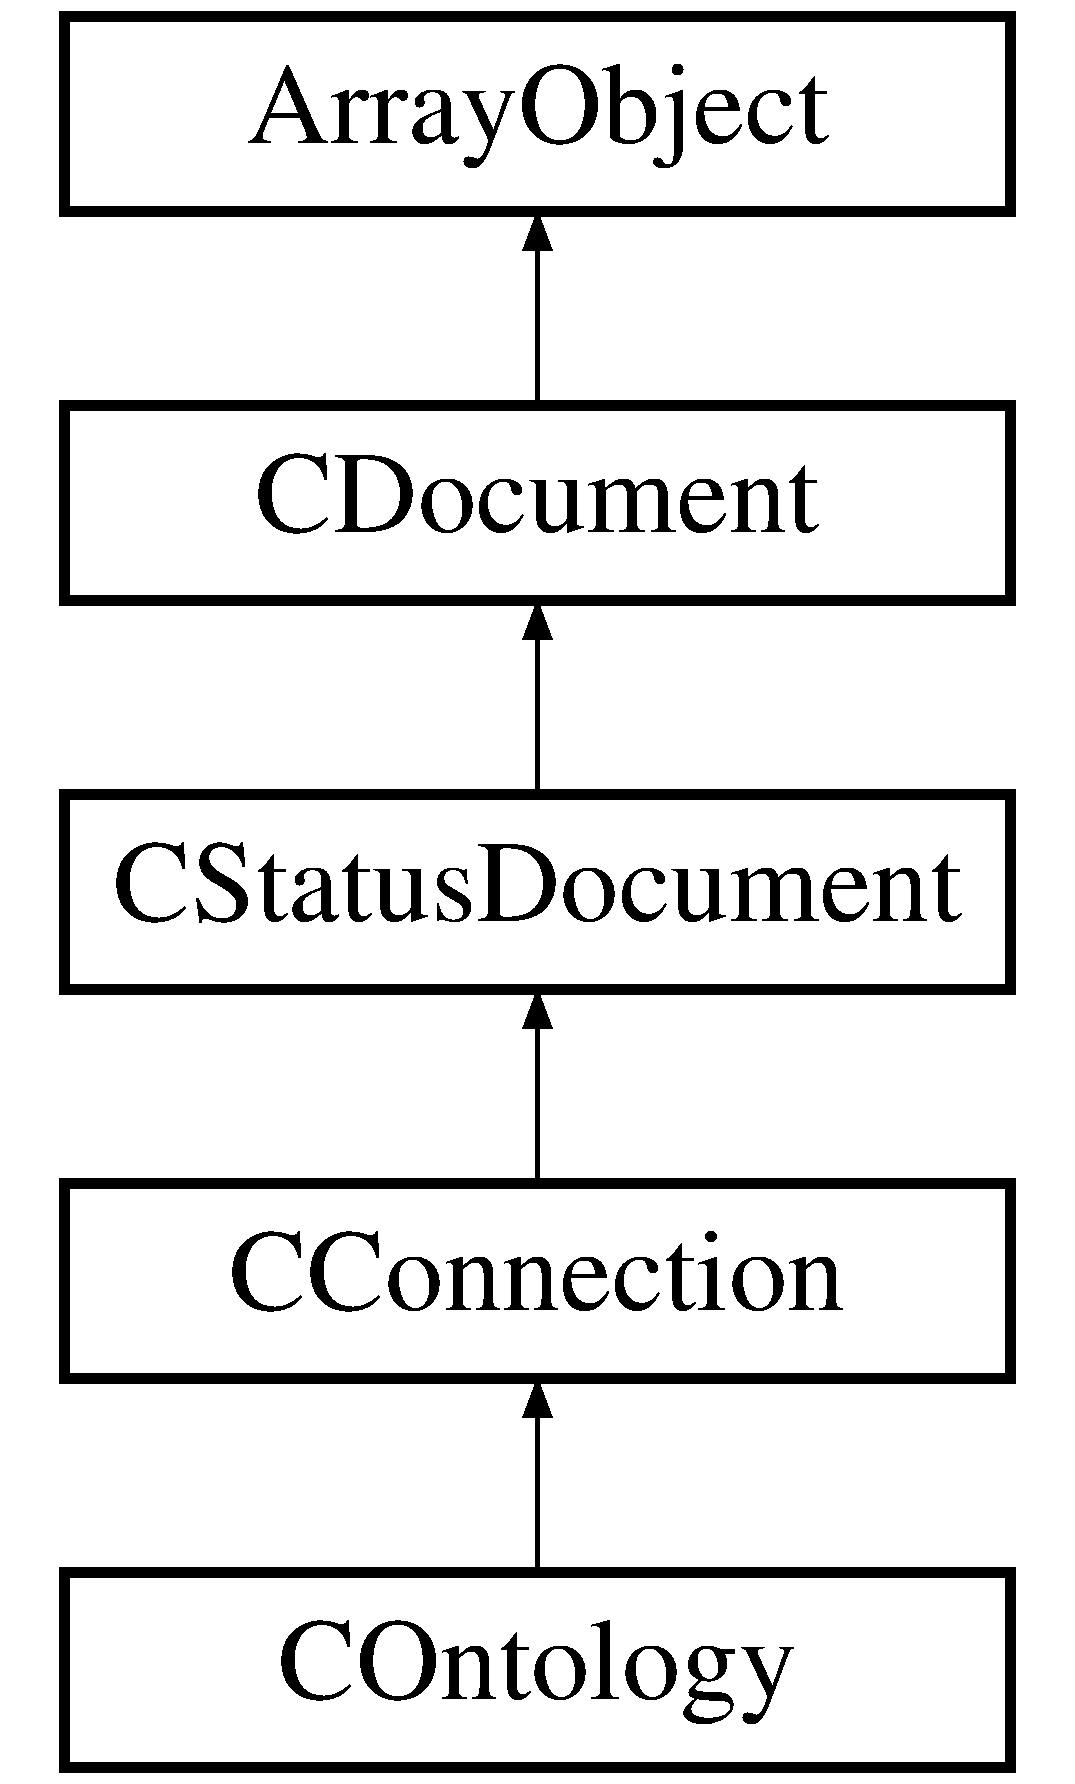
\includegraphics[height=5.000000cm]{class_c_ontology}
\end{center}
\end{figure}
\subsection*{Public Member Functions}
\begin{DoxyCompactItemize}
\item 
\hyperlink{class_c_ontology_a3bf6307b3353401050f4e66822d4cecf}{\-\_\-\-\_\-to\-String} ()
\item 
\hyperlink{class_c_ontology_a1c7acc74d753c47dc89d46464afc0099}{Connection} (\$the\-Value=N\-U\-L\-L, \$get\-Old=F\-A\-L\-S\-E)
\item 
\hyperlink{class_c_ontology_ae8905b152a35d927137faeb2aa1885ce}{Get\-Database} ()
\item 
\hyperlink{class_c_ontology_a305fa41da58da8239b7636e0ffdc9689}{Init\-Containers} ()
\item 
\hyperlink{class_c_ontology_a6bfd3100a83783cf1997749bf901b8df}{Init\-Ontology} ()
\item 
\hyperlink{class_c_ontology_ad9b6ebbaf592ab0543be3f63cddd025c}{Load\-X\-M\-L\-Ontology\-File} (\$the\-File\-Path)
\item 
\hyperlink{class_c_ontology_a146da417467dc53827e4b1a2e8646276}{Get\-Template\-Array} (\$the\-Root, \$the\-Language)
\item 
\hyperlink{class_c_ontology_a03d99559d6b357d64a6437a68d157c26}{Get\-Excel\-Template} (\$the\-Root, \$the\-Language, \$the\-Path=N\-U\-L\-L)
\item 
\hyperlink{class_c_ontology_a9789841620a6b75f09120223d7fd4dc8}{Load\-I\-S\-O\-P\-O\-Files} ()
\item 
\hyperlink{class_c_ontology_a85ac5a51432b48fe5c2fa81a6fae2c0a}{Set\-All\-Countries} (\$the\-Enumeration)
\item 
\hyperlink{class_c_ontology_ab00174cd1bb4ddd57457ad5dbc7db4da}{\-\_\-\-Get\-Template} (\&\$the\-Template, \hyperlink{class_c_database}{C\-Database} \$the\-Database, \hyperlink{class_c_ontology_term}{C\-Ontology\-Term} \$the\-Predicate, \hyperlink{class_c_ontology_node}{C\-Ontology\-Node} \$the\-Node, \$the\-Language, \&\$the\-Cache)
\end{DoxyCompactItemize}
\subsection*{Protected Member Functions}
\begin{DoxyCompactItemize}
\item 
\hyperlink{class_c_ontology_ae3e06b7824d7b902bd7bd5c9d393ab8a}{\-\_\-\-Load\-X\-M\-L\-Ontology\-Unit} (\hyperlink{class_c_database}{C\-Database} \$the\-Database, Simple\-X\-M\-L\-Element \$the\-Unit)
\item 
\hyperlink{class_c_ontology_af0ce6bf134670c99a34d23ff1643ff09}{\-\_\-\-Load\-X\-M\-L\-Ontology\-Term} (\&\$the\-Cache, \hyperlink{class_c_database}{C\-Database} \$the\-Database, Simple\-X\-M\-L\-Element \$the\-Element)
\item 
\hyperlink{class_c_ontology_a08a3e787742fde631feaefe426602e6f}{\-\_\-\-Load\-X\-M\-L\-Ontology\-Node} (\&\$the\-Cache, \hyperlink{class_c_database}{C\-Database} \$the\-Database, Simple\-X\-M\-L\-Element \$the\-Element)
\item 
\hyperlink{class_c_ontology_a736efd02f870b97c6cffcd73bcc4c16b}{\-\_\-\-Load\-X\-M\-L\-Ontology\-Edge} (\&\$the\-Cache, \hyperlink{class_c_database}{C\-Database} \$the\-Database, Simple\-X\-M\-L\-Element \$the\-Element)
\item 
\hyperlink{class_c_ontology_a889fdf93b0cf4cbf631e4cfd64006e5f}{\-\_\-\-Load\-X\-M\-L\-Ontology\-Tag} (\&\$the\-Cache, \hyperlink{class_c_database}{C\-Database} \$the\-Database, Simple\-X\-M\-L\-Element \$the\-Element)
\item 
\hyperlink{class_c_ontology_add240f87c2864b092a1435cac49d0647}{\-\_\-\-Resolve\-Ontology\-Node} (\hyperlink{class_c_database}{C\-Database} \$the\-Database, Simple\-X\-M\-L\-Element \$the\-Element)
\item 
\hyperlink{class_c_ontology_a09272a637e5f3edb5575253ff6127faa}{\-\_\-\-I\-S\-O\-Decode\-P\-O\-Files} ()
\item 
\hyperlink{class_c_ontology_a8bdcf5f69b661f7e714db4ff3f706302}{\-\_\-\-I\-S\-O\-Parse\-X\-M\-L\-Files} (\hyperlink{class_c_database}{C\-Database} \$the\-Database)
\item 
\hyperlink{class_c_ontology_a1cc310175e0b77d130f7e540c00a1772}{\-\_\-\-I\-S\-O\-Parse6393\-X\-M\-L} (\hyperlink{class_c_database}{C\-Database} \$the\-Database)
\item 
\hyperlink{class_c_ontology_adb0eec614edf29dd1986634fa4884ba3}{\-\_\-\-I\-S\-O\-Parse639\-X\-M\-L} (\hyperlink{class_c_database}{C\-Database} \$the\-Database)
\item 
\hyperlink{class_c_ontology_a11b4fd10984fec1ec88b450ff8623fcc}{\-\_\-\-I\-S\-O\-Parse31661\-X\-M\-L} (\hyperlink{class_c_database}{C\-Database} \$the\-Database)
\item 
\hyperlink{class_c_ontology_af784ce9c04c61d438da744c7337f7284}{\-\_\-\-I\-S\-O\-Parse31663\-X\-M\-L} (\hyperlink{class_c_database}{C\-Database} \$the\-Database)
\item 
\hyperlink{class_c_ontology_af9a15784b11030134a1504e22fc5ea4f}{\-\_\-\-I\-S\-O\-Parse31662\-X\-M\-L} (\hyperlink{class_c_database}{C\-Database} \$the\-Database)
\item 
\hyperlink{class_c_ontology_aee3fc6563229a9e9565c9e78294af8ed}{\-\_\-\-I\-S\-O\-Parse4217\-X\-M\-L} (\hyperlink{class_c_database}{C\-Database} \$the\-Database)
\item 
\hyperlink{class_c_ontology_a0fdf66940951cf5ccd13d21b9bf3e114}{\-\_\-\-I\-S\-O\-Parse15924\-X\-M\-L} (\hyperlink{class_c_database}{C\-Database} \$the\-Database)
\item 
\hyperlink{class_c_ontology_a537ac00b77db44b312c4e46ba4869eb5}{\-\_\-\-I\-S\-O\-Collect\-Language\-Strings} (\hyperlink{class_c_persistent_object}{C\-Persistent\-Object} \$the\-Object, \$the\-File, \$the\-Tags)
\end{DoxyCompactItemize}
\subsection*{Additional Inherited Members}


\subsection{Member Function Documentation}
\hypertarget{class_c_ontology_a3bf6307b3353401050f4e66822d4cecf}{\index{C\-Ontology@{C\-Ontology}!\-\_\-\-\_\-to\-String@{\-\_\-\-\_\-to\-String}}
\index{\-\_\-\-\_\-to\-String@{\-\_\-\-\_\-to\-String}!COntology@{C\-Ontology}}
\subsubsection[{\-\_\-\-\_\-to\-String}]{\setlength{\rightskip}{0pt plus 5cm}C\-Ontology\-::\-\_\-\-\_\-to\-String (
\begin{DoxyParamCaption}
{}
\end{DoxyParamCaption}
)}}\label{class_c_ontology_a3bf6307b3353401050f4e66822d4cecf}
\subparagraph*{Return connection name}

We implement this method by letting the connection object take care of returning its name.

public \begin{DoxyReturn}{Returns}
string The connection name.
\end{DoxyReturn}
\hyperlink{class_c_ontology_a1c7acc74d753c47dc89d46464afc0099}{Connection()} \hypertarget{class_c_ontology_ab00174cd1bb4ddd57457ad5dbc7db4da}{\index{C\-Ontology@{C\-Ontology}!\-\_\-\-Get\-Template@{\-\_\-\-Get\-Template}}
\index{\-\_\-\-Get\-Template@{\-\_\-\-Get\-Template}!COntology@{C\-Ontology}}
\subsubsection[{\-\_\-\-Get\-Template}]{\setlength{\rightskip}{0pt plus 5cm}C\-Ontology\-::\-\_\-\-Get\-Template (
\begin{DoxyParamCaption}
\item[{\&}]{\$the\-Template, }
\item[{{\bf C\-Database}}]{\$the\-Database, }
\item[{{\bf C\-Ontology\-Term}}]{\$the\-Predicate, }
\item[{{\bf C\-Ontology\-Node}}]{\$the\-Node, }
\item[{}]{\$the\-Language, }
\item[{\&}]{\$the\-Cache}
\end{DoxyParamCaption}
)}}\label{class_c_ontology_ab00174cd1bb4ddd57457ad5dbc7db4da}
\subparagraph*{Create template}

This method will check whether the received node corresponds to a tag feature, in that case it will add the tag's info to the provided template array, if not, it will recurse on all nodes related to the provided node by the provided predicate.

The method expects the following parameters\-:


\begin{DoxyItemize}
\item {\ttfamily \&\$the\-Template}\-: An array reference that will receive the list of templates. 
\item {\ttfamily \$the\-Database}\-: Database connection. 
\item {\ttfamily \$the\-Predicate}\-: Relationship predicate term object. 
\item {\ttfamily \$the\-Node}\-: Node to be checked. 
\item {\ttfamily \$the\-Language}\-: Language of labels and definitions. 
\end{DoxyItemize}

The provided template array reference will be filled with elements structured as follows\-:


\begin{DoxyItemize}
\item {\ttfamily 0}\-: This index will hold the tag global identifier. 
\item {\ttfamily 1}\-: This index will hold the tag labels of all path elements separated by a carriage return character. 
\item {\ttfamily 2}\-: This index will hold the tag definitions of all vertex path elements separated by a carriage return character. 
\item {\itshape other}\-: All subsequent elements will hold the respective path term global identifiers. 
\end{DoxyItemize}


\begin{DoxyParams}[1]{Parameters}
reference & {\em \&\$the\-Template} & Receives template. \\
\hline
\hyperlink{class_c_database}{C\-Database} & {\em \$the\-Database} & Database connection. \\
\hline
\hyperlink{class_c_ontology_term}{C\-Ontology\-Term} & {\em \$the\-Predicate} & Predicate term. \\
\hline
\hyperlink{class_c_ontology_node}{C\-Ontology\-Node} & {\em \$the\-Node} & Node to be checked. \\
\hline
string & {\em \$the\-Language} & Language code. \\
\hline
reference & {\em \&\$the\-Cache} & P\-R\-I\-V\-A\-T\-E.\\
\hline
\end{DoxyParams}
public


\begin{DoxyExceptions}{Exceptions}
{\em Exception} & \\
\hline
\end{DoxyExceptions}
\hypertarget{class_c_ontology_a537ac00b77db44b312c4e46ba4869eb5}{\index{C\-Ontology@{C\-Ontology}!\-\_\-\-I\-S\-O\-Collect\-Language\-Strings@{\-\_\-\-I\-S\-O\-Collect\-Language\-Strings}}
\index{\-\_\-\-I\-S\-O\-Collect\-Language\-Strings@{\-\_\-\-I\-S\-O\-Collect\-Language\-Strings}!COntology@{C\-Ontology}}
\subsubsection[{\-\_\-\-I\-S\-O\-Collect\-Language\-Strings}]{\setlength{\rightskip}{0pt plus 5cm}C\-Ontology\-::\-\_\-\-I\-S\-O\-Collect\-Language\-Strings (
\begin{DoxyParamCaption}
\item[{{\bf C\-Persistent\-Object}}]{\$the\-Object, }
\item[{}]{\$the\-File, }
\item[{}]{\$the\-Tags}
\end{DoxyParamCaption}
)\hspace{0.3cm}{\ttfamily [protected]}}}\label{class_c_ontology_a537ac00b77db44b312c4e46ba4869eb5}
\subparagraph*{Collect language strings}

This method will iterate all language files and add the corresponding language strings to the provided object.

The method expects two parameters\-: the object to be updated and an array of tags to be checked.


\begin{DoxyParams}[1]{Parameters}
\hyperlink{class_c_persistent_object}{C\-Persistent\-Object} & {\em \$the\-Object} & Object to be updated. \\
\hline
string & {\em \$the\-File} & File body name. \\
\hline
array & {\em \$the\-Tags} & List of tags to check.\\
\hline
\end{DoxyParams}
protected \hypertarget{class_c_ontology_a09272a637e5f3edb5575253ff6127faa}{\index{C\-Ontology@{C\-Ontology}!\-\_\-\-I\-S\-O\-Decode\-P\-O\-Files@{\-\_\-\-I\-S\-O\-Decode\-P\-O\-Files}}
\index{\-\_\-\-I\-S\-O\-Decode\-P\-O\-Files@{\-\_\-\-I\-S\-O\-Decode\-P\-O\-Files}!COntology@{C\-Ontology}}
\subsubsection[{\-\_\-\-I\-S\-O\-Decode\-P\-O\-Files}]{\setlength{\rightskip}{0pt plus 5cm}C\-Ontology\-::\-\_\-\-I\-S\-O\-Decode\-P\-O\-Files (
\begin{DoxyParamCaption}
{}
\end{DoxyParamCaption}
)\hspace{0.3cm}{\ttfamily [protected]}}}\label{class_c_ontology_a09272a637e5f3edb5575253ff6127faa}
\subparagraph*{Decode P\-O files}

This method will parse all M\-O files, decode them into P\-O files and write to the \hyperlink{}{k\-I\-S\-O\-\_\-\-F\-I\-L\-E\-\_\-\-P\-O\-\_\-\-D\-I\-R} directory the P\-H\-P serialised decode array.

protected


\begin{DoxyExceptions}{Exceptions}
{\em Exception} & \\
\hline
\end{DoxyExceptions}
\hypertarget{class_c_ontology_a0fdf66940951cf5ccd13d21b9bf3e114}{\index{C\-Ontology@{C\-Ontology}!\-\_\-\-I\-S\-O\-Parse15924\-X\-M\-L@{\-\_\-\-I\-S\-O\-Parse15924\-X\-M\-L}}
\index{\-\_\-\-I\-S\-O\-Parse15924\-X\-M\-L@{\-\_\-\-I\-S\-O\-Parse15924\-X\-M\-L}!COntology@{C\-Ontology}}
\subsubsection[{\-\_\-\-I\-S\-O\-Parse15924\-X\-M\-L}]{\setlength{\rightskip}{0pt plus 5cm}C\-Ontology\-::\-\_\-\-I\-S\-O\-Parse15924\-X\-M\-L (
\begin{DoxyParamCaption}
\item[{{\bf C\-Database}}]{\$the\-Database}
\end{DoxyParamCaption}
)\hspace{0.3cm}{\ttfamily [protected]}}}\label{class_c_ontology_a0fdf66940951cf5ccd13d21b9bf3e114}
\subparagraph*{Parse I\-S\-O 15924 X\-M\-L file}

This method will parse the X\-M\-L I\-S\-O 15924 file.

The method will load the following attributes\-:


\begin{DoxyItemize}
\item {\ttfamily I\-S\-O\-:15924\-:alpha-\/4}\-: Alpha-\/4 code \mbox{[}{\ttfamily alpha\-\_\-4\-\_\-code}\mbox{]}. 
\item {\ttfamily I\-S\-O\-:15924\-:numeric}\-: Alpha-\/4 code \mbox{[}{\ttfamily numeric\-\_\-code}\mbox{]}. 
\item {\ttfamily \hyperlink{}{k\-T\-A\-G\-\_\-\-L\-A\-B\-E\-L}/tt$>$\-: \mbox{[}{\ttfamily name}\mbox{]}. }
\end{DoxyItemize}

{\ttfamily 
\begin{DoxyParams}[1]{Parameters}
\hyperlink{class_c_database}{C\-Database} & {\em \$the\-Database} & Database container.\\
\hline
\end{DoxyParams}
protected}

{\ttfamily 
\begin{DoxyExceptions}{Exceptions}
{\em Exception} & \\
\hline
\end{DoxyExceptions}
}\hypertarget{class_c_ontology_a11b4fd10984fec1ec88b450ff8623fcc}{\index{C\-Ontology@{C\-Ontology}!\-\_\-\-I\-S\-O\-Parse31661\-X\-M\-L@{\-\_\-\-I\-S\-O\-Parse31661\-X\-M\-L}}
\index{\-\_\-\-I\-S\-O\-Parse31661\-X\-M\-L@{\-\_\-\-I\-S\-O\-Parse31661\-X\-M\-L}!COntology@{C\-Ontology}}
\subsubsection[{\-\_\-\-I\-S\-O\-Parse31661\-X\-M\-L}]{\setlength{\rightskip}{0pt plus 5cm}C\-Ontology\-::\-\_\-\-I\-S\-O\-Parse31661\-X\-M\-L (
\begin{DoxyParamCaption}
\item[{{\bf C\-Database}}]{\$the\-Database}
\end{DoxyParamCaption}
)\hspace{0.3cm}{\ttfamily [protected]}}}\label{class_c_ontology_a11b4fd10984fec1ec88b450ff8623fcc}
\subparagraph*{Parse I\-S\-O 3166-\/1 X\-M\-L file}

This method will parse the X\-M\-L I\-S\-O 3166-\/1 file.

The method will load the following attributes\-:


\begin{DoxyItemize}
\item {\ttfamily I\-S\-O\-:3166\-:alpha-\/3}\-: Alpha 3 code \mbox{[}{\ttfamily alpha\-\_\-3\-\_\-code}\mbox{]}. 
\item {\ttfamily I\-S\-O\-:3166\-:alpha-\/2}\-: Alpha 2 code \mbox{[}{\ttfamily alpha\-\_\-2\-\_\-code}\mbox{]}. 
\item {\ttfamily I\-S\-O\-:3166\-:numeric}\-: Numeric code \mbox{[}{\ttfamily numeric\-\_\-code}\mbox{]}. 
\item {\ttfamily \hyperlink{}{k\-T\-A\-G\-\_\-\-L\-A\-B\-E\-L}/tt$>$\-: Label {\ttfamily name} \mbox{[}{\ttfamily name}\mbox{]}. }
\item {\ttfamily {\ttfamily \hyperlink{}{k\-T\-A\-G\-\_\-\-D\-E\-F\-I\-N\-I\-T\-I\-O\-N}/tt$>$\-: Definition \mbox{[}{\ttfamily official\-\_\-name}\mbox{]}. }}
\item {\ttfamily {\ttfamily {\ttfamily I\-S\-O\-:3166\-:common\-\_\-name}\-: Common name \mbox{[}{\ttfamily common\-\_\-name}\mbox{]}. }}
\end{DoxyItemize}

{\ttfamily {\ttfamily 
\begin{DoxyParams}[1]{Parameters}
\hyperlink{class_c_database}{C\-Database} & {\em \$the\-Database} & Database container.\\
\hline
\end{DoxyParams}
protected}}

{\ttfamily {\ttfamily 
\begin{DoxyExceptions}{Exceptions}
{\em Exception} & \\
\hline
\end{DoxyExceptions}
}}\hypertarget{class_c_ontology_af9a15784b11030134a1504e22fc5ea4f}{\index{C\-Ontology@{C\-Ontology}!\-\_\-\-I\-S\-O\-Parse31662\-X\-M\-L@{\-\_\-\-I\-S\-O\-Parse31662\-X\-M\-L}}
\index{\-\_\-\-I\-S\-O\-Parse31662\-X\-M\-L@{\-\_\-\-I\-S\-O\-Parse31662\-X\-M\-L}!COntology@{C\-Ontology}}
\subsubsection[{\-\_\-\-I\-S\-O\-Parse31662\-X\-M\-L}]{\setlength{\rightskip}{0pt plus 5cm}C\-Ontology\-::\-\_\-\-I\-S\-O\-Parse31662\-X\-M\-L (
\begin{DoxyParamCaption}
\item[{{\bf C\-Database}}]{\$the\-Database}
\end{DoxyParamCaption}
)\hspace{0.3cm}{\ttfamily [protected]}}}\label{class_c_ontology_af9a15784b11030134a1504e22fc5ea4f}
\subparagraph*{Parse I\-S\-O 3166-\/2 X\-M\-L file}

This method will parse the X\-M\-L I\-S\-O 3166-\/2 file.

The method will load the following attributes\-:


\begin{DoxyItemize}
\item {\ttfamily I\-S\-O\-:3166\-:1\-:alpha-\/2}\-: Alpha 2 code \mbox{[}{\ttfamily iso\-\_\-3166\-\_\-country\mbox{[}code\mbox{]}}\mbox{]}. 
\item {\ttfamily I\-S\-O\-:3166\-:2\-:type}\-: Type \mbox{[}{\ttfamily iso\-\_\-3166\-\_\-subset\mbox{[}type\mbox{]}}\mbox{]}. 
\item {\ttfamily I\-S\-O\-:3166\-:2}\-: Type \mbox{[}{\ttfamily iso\-\_\-3166\-\_\-subset\mbox{[}type\mbox{]}}\mbox{]}. 
\item {\ttfamily \hyperlink{}{k\-T\-A\-G\-\_\-\-L\-A\-B\-E\-L}/tt$>$\-: Label {\ttfamily name} \mbox{[}{\ttfamily name}\mbox{]}. }
\item {\ttfamily {\ttfamily \hyperlink{}{k\-T\-A\-G\-\_\-\-D\-E\-F\-I\-N\-I\-T\-I\-O\-N}/tt$>$\-: Definition \mbox{[}{\ttfamily official\-\_\-name}\mbox{]}. }}
\item {\ttfamily {\ttfamily {\ttfamily I\-S\-O\-:3166\-:common\-\_\-name}\-: Common name \mbox{[}{\ttfamily common\-\_\-name}\mbox{]}. }}
\end{DoxyItemize}

{\ttfamily {\ttfamily 
\begin{DoxyParams}[1]{Parameters}
\hyperlink{class_c_database}{C\-Database} & {\em \$the\-Database} & Database container.\\
\hline
\end{DoxyParams}
protected}}

{\ttfamily {\ttfamily 
\begin{DoxyExceptions}{Exceptions}
{\em Exception} & \\
\hline
\end{DoxyExceptions}
}}\hypertarget{class_c_ontology_af784ce9c04c61d438da744c7337f7284}{\index{C\-Ontology@{C\-Ontology}!\-\_\-\-I\-S\-O\-Parse31663\-X\-M\-L@{\-\_\-\-I\-S\-O\-Parse31663\-X\-M\-L}}
\index{\-\_\-\-I\-S\-O\-Parse31663\-X\-M\-L@{\-\_\-\-I\-S\-O\-Parse31663\-X\-M\-L}!COntology@{C\-Ontology}}
\subsubsection[{\-\_\-\-I\-S\-O\-Parse31663\-X\-M\-L}]{\setlength{\rightskip}{0pt plus 5cm}C\-Ontology\-::\-\_\-\-I\-S\-O\-Parse31663\-X\-M\-L (
\begin{DoxyParamCaption}
\item[{{\bf C\-Database}}]{\$the\-Database}
\end{DoxyParamCaption}
)\hspace{0.3cm}{\ttfamily [protected]}}}\label{class_c_ontology_af784ce9c04c61d438da744c7337f7284}
\subparagraph*{Parse I\-S\-O 3166-\/3 X\-M\-L file}

This method will parse the X\-M\-L I\-S\-O 3166-\/3 file.

The method will load the following attributes\-:


\begin{DoxyItemize}
\item {\ttfamily I\-S\-O\-:3166\-:1\-:alpha-\/3}\-: Alpha 3 code \mbox{[}{\ttfamily alpha\-\_\-3\-\_\-code}\mbox{]}. 
\item {\ttfamily I\-S\-O\-:3166\-:1\-:alpha-\/4}\-: Alpha 4 code \mbox{[}{\ttfamily alpha\-\_\-4\-\_\-code}\mbox{]}. 
\item {\ttfamily I\-S\-O\-:3166\-:1\-:numeric}\-: Numeric code \mbox{[}{\ttfamily numeric\-\_\-code}\mbox{]}. 
\item {\ttfamily \hyperlink{}{k\-T\-A\-G\-\_\-\-L\-A\-B\-E\-L}/tt$>$\-: Label {\ttfamily name} \mbox{[}{\ttfamily names}\mbox{]}. }
\item {\ttfamily {\ttfamily \hyperlink{}{k\-T\-A\-G\-\_\-\-D\-E\-F\-I\-N\-I\-T\-I\-O\-N}/tt$>$\-: Definition \mbox{[}{\ttfamily comment}\mbox{]}. }}
\item {\ttfamily {\ttfamily {\ttfamily I\-S\-O\-:attributes\-:date\-\_\-withdrawn}\-: Date withdrawn \mbox{[}{\ttfamily date\-\_\-withdrawn}\mbox{]}. }}
\end{DoxyItemize}

{\ttfamily {\ttfamily 
\begin{DoxyParams}[1]{Parameters}
\hyperlink{class_c_database}{C\-Database} & {\em \$the\-Database} & Database container.\\
\hline
\end{DoxyParams}
protected}}

{\ttfamily {\ttfamily 
\begin{DoxyExceptions}{Exceptions}
{\em Exception} & \\
\hline
\end{DoxyExceptions}
}}\hypertarget{class_c_ontology_aee3fc6563229a9e9565c9e78294af8ed}{\index{C\-Ontology@{C\-Ontology}!\-\_\-\-I\-S\-O\-Parse4217\-X\-M\-L@{\-\_\-\-I\-S\-O\-Parse4217\-X\-M\-L}}
\index{\-\_\-\-I\-S\-O\-Parse4217\-X\-M\-L@{\-\_\-\-I\-S\-O\-Parse4217\-X\-M\-L}!COntology@{C\-Ontology}}
\subsubsection[{\-\_\-\-I\-S\-O\-Parse4217\-X\-M\-L}]{\setlength{\rightskip}{0pt plus 5cm}C\-Ontology\-::\-\_\-\-I\-S\-O\-Parse4217\-X\-M\-L (
\begin{DoxyParamCaption}
\item[{{\bf C\-Database}}]{\$the\-Database}
\end{DoxyParamCaption}
)\hspace{0.3cm}{\ttfamily [protected]}}}\label{class_c_ontology_aee3fc6563229a9e9565c9e78294af8ed}
\subparagraph*{Parse I\-S\-O 4217 X\-M\-L file}

This method will parse the X\-M\-L I\-S\-O 4217 file.

The method will load the following attributes\-:


\begin{DoxyItemize}
\item {\ttfamily I\-S\-O\-:4217\-:A}\-: Active \mbox{[}{\ttfamily letter\-\_\-code}\mbox{]}. 
\item {\ttfamily I\-S\-O\-:4217\-:H}\-: Historic \mbox{[}{\ttfamily letter\-\_\-code}\mbox{]}. 
\item {\ttfamily I\-S\-O\-:4217\-:A}\-: Active \mbox{[}{\ttfamily numeric\-\_\-code}\mbox{]}. 
\item {\ttfamily I\-S\-O\-:4217\-:H}\-: Historic \mbox{[}{\ttfamily numeric\-\_\-code}\mbox{]}. 
\item {\ttfamily \hyperlink{}{k\-T\-A\-G\-\_\-\-L\-A\-B\-E\-L}/tt$>$\-: \mbox{[}{\ttfamily currency\-\_\-name}\mbox{]}. }
\item {\ttfamily {\ttfamily I\-S\-O\-:attributes\-:date\-\_\-withdrawn}\-: Date withdrawn \mbox{[}{\ttfamily date\-\_\-withdrawn}\mbox{]}. }
\end{DoxyItemize}

{\ttfamily 
\begin{DoxyParams}[1]{Parameters}
\hyperlink{class_c_database}{C\-Database} & {\em \$the\-Database} & Database container.\\
\hline
\end{DoxyParams}
protected}

{\ttfamily 
\begin{DoxyExceptions}{Exceptions}
{\em Exception} & \\
\hline
\end{DoxyExceptions}
}\hypertarget{class_c_ontology_a1cc310175e0b77d130f7e540c00a1772}{\index{C\-Ontology@{C\-Ontology}!\-\_\-\-I\-S\-O\-Parse6393\-X\-M\-L@{\-\_\-\-I\-S\-O\-Parse6393\-X\-M\-L}}
\index{\-\_\-\-I\-S\-O\-Parse6393\-X\-M\-L@{\-\_\-\-I\-S\-O\-Parse6393\-X\-M\-L}!COntology@{C\-Ontology}}
\subsubsection[{\-\_\-\-I\-S\-O\-Parse6393\-X\-M\-L}]{\setlength{\rightskip}{0pt plus 5cm}C\-Ontology\-::\-\_\-\-I\-S\-O\-Parse6393\-X\-M\-L (
\begin{DoxyParamCaption}
\item[{{\bf C\-Database}}]{\$the\-Database}
\end{DoxyParamCaption}
)\hspace{0.3cm}{\ttfamily [protected]}}}\label{class_c_ontology_a1cc310175e0b77d130f7e540c00a1772}
\subparagraph*{Parse I\-S\-O 639-\/3 X\-M\-L files}

This method will parse the X\-M\-L I\-S\-O 639-\/3 files.

The method will load the following attributes\-:


\begin{DoxyItemize}
\item {\ttfamily I\-S\-O\-:639\-:1}\-: Part 1 code \mbox{[}{\ttfamily part1\-\_\-code}\mbox{]}. 
\item {\ttfamily I\-S\-O\-:639\-:2}\-: Part 2 code \mbox{[}{\ttfamily part2\-\_\-code}\mbox{]}. 
\item {\ttfamily I\-S\-O\-:639\-:3}\-: Part 3 code \mbox{[}{\ttfamily id}\mbox{]}. 
\item {\ttfamily I\-S\-O\-:639\-:status}\-: Status \mbox{[}{\ttfamily status}\mbox{]}. 
\item {\ttfamily I\-S\-O\-:639\-:scope}\-: Scope \mbox{[}{\ttfamily scope}\mbox{]}. 
\item {\ttfamily I\-S\-O\-:639\-:type}\-: Type \mbox{[}{\ttfamily type}\mbox{]}. 
\item {\ttfamily I\-S\-O\-:639\-:inverted\-\_\-name}\-: Inverted name \mbox{[}{\ttfamily inverted\-\_\-name}\mbox{]}. 
\item {\ttfamily I\-S\-O\-:639\-:common\-\_\-name}\-: Common name \mbox{[}{\ttfamily common\-\_\-name}\mbox{]}. 
\item {\ttfamily \hyperlink{}{k\-T\-A\-G\-\_\-\-L\-A\-B\-E\-L}/tt$>$\-: Label {\ttfamily name} \mbox{[}{\ttfamily name}\mbox{]}. }
\item {\ttfamily {\ttfamily \hyperlink{}{k\-T\-A\-G\-\_\-\-D\-E\-F\-I\-N\-I\-T\-I\-O\-N}/tt$>$\-: Definition \mbox{[}{\ttfamily reference\-\_\-name}\mbox{]}. }}
\end{DoxyItemize}

{\ttfamily {\ttfamily 
\begin{DoxyParams}[1]{Parameters}
\hyperlink{class_c_database}{C\-Database} & {\em \$the\-Database} & Database container.\\
\hline
\end{DoxyParams}
protected}}

{\ttfamily {\ttfamily 
\begin{DoxyExceptions}{Exceptions}
{\em Exception} & \\
\hline
\end{DoxyExceptions}
}}\hypertarget{class_c_ontology_adb0eec614edf29dd1986634fa4884ba3}{\index{C\-Ontology@{C\-Ontology}!\-\_\-\-I\-S\-O\-Parse639\-X\-M\-L@{\-\_\-\-I\-S\-O\-Parse639\-X\-M\-L}}
\index{\-\_\-\-I\-S\-O\-Parse639\-X\-M\-L@{\-\_\-\-I\-S\-O\-Parse639\-X\-M\-L}!COntology@{C\-Ontology}}
\subsubsection[{\-\_\-\-I\-S\-O\-Parse639\-X\-M\-L}]{\setlength{\rightskip}{0pt plus 5cm}C\-Ontology\-::\-\_\-\-I\-S\-O\-Parse639\-X\-M\-L (
\begin{DoxyParamCaption}
\item[{{\bf C\-Database}}]{\$the\-Database}
\end{DoxyParamCaption}
)\hspace{0.3cm}{\ttfamily [protected]}}}\label{class_c_ontology_adb0eec614edf29dd1986634fa4884ba3}
\subparagraph*{Parse I\-S\-O 639 X\-M\-L files}

This method will parse the X\-M\-L I\-S\-O 639 files.

The method will load the following attributes\-:


\begin{DoxyItemize}
\item {\ttfamily I\-S\-O\-:639\-:1}\-: Part 1 code \mbox{[}{\ttfamily iso\-\_\-639\-\_\-1\-\_\-code}\mbox{]} (as reference). 
\item {\ttfamily I\-S\-O\-:639\-:2\-B}\-: Part 2\-B code \mbox{[}{\ttfamily iso\-\_\-639\-\_\-2\-B\-\_\-code}\mbox{]}. 
\item {\ttfamily I\-S\-O\-:639\-:2\-T}\-: Part 2\-T code \mbox{[}{\ttfamily iso\-\_\-639\-\_\-2\-T\-\_\-code}\mbox{]}. 
\item {\ttfamily I\-S\-O\-:639\-:inverted\-\_\-name}\-: Inverted name \mbox{[}{\ttfamily inverted\-\_\-name}\mbox{]}. 
\item {\ttfamily \hyperlink{}{k\-T\-A\-G\-\_\-\-L\-A\-B\-E\-L}/tt$>$\-: Label {\ttfamily name} \mbox{[}{\ttfamily name}\mbox{]}. This is used only if the part 1 code is not found. }
\item {\ttfamily {\ttfamily \hyperlink{}{k\-T\-A\-G\-\_\-\-D\-E\-F\-I\-N\-I\-T\-I\-O\-N}/tt$>$\-: Definition \mbox{[}{\ttfamily reference\-\_\-name}\mbox{]}. This is used only if the part 1 code is not found. }}
\end{DoxyItemize}

{\ttfamily {\ttfamily 
\begin{DoxyParams}[1]{Parameters}
\hyperlink{class_c_database}{C\-Database} & {\em \$the\-Database} & Database container.\\
\hline
\end{DoxyParams}
protected}}

{\ttfamily {\ttfamily 
\begin{DoxyExceptions}{Exceptions}
{\em Exception} & \\
\hline
\end{DoxyExceptions}
}}\hypertarget{class_c_ontology_a8bdcf5f69b661f7e714db4ff3f706302}{\index{C\-Ontology@{C\-Ontology}!\-\_\-\-I\-S\-O\-Parse\-X\-M\-L\-Files@{\-\_\-\-I\-S\-O\-Parse\-X\-M\-L\-Files}}
\index{\-\_\-\-I\-S\-O\-Parse\-X\-M\-L\-Files@{\-\_\-\-I\-S\-O\-Parse\-X\-M\-L\-Files}!COntology@{C\-Ontology}}
\subsubsection[{\-\_\-\-I\-S\-O\-Parse\-X\-M\-L\-Files}]{\setlength{\rightskip}{0pt plus 5cm}C\-Ontology\-::\-\_\-\-I\-S\-O\-Parse\-X\-M\-L\-Files (
\begin{DoxyParamCaption}
\item[{{\bf C\-Database}}]{\$the\-Database}
\end{DoxyParamCaption}
)\hspace{0.3cm}{\ttfamily [protected]}}}\label{class_c_ontology_a8bdcf5f69b661f7e714db4ff3f706302}
\subparagraph*{Parse X\-M\-L files}

This method will parse the X\-M\-L files and store the data in the database.


\begin{DoxyParams}[1]{Parameters}
\hyperlink{class_c_database}{C\-Database} & {\em \$the\-Database} & Database container.\\
\hline
\end{DoxyParams}
protected


\begin{DoxyExceptions}{Exceptions}
{\em Exception} & \\
\hline
\end{DoxyExceptions}
\hypertarget{class_c_ontology_a736efd02f870b97c6cffcd73bcc4c16b}{\index{C\-Ontology@{C\-Ontology}!\-\_\-\-Load\-X\-M\-L\-Ontology\-Edge@{\-\_\-\-Load\-X\-M\-L\-Ontology\-Edge}}
\index{\-\_\-\-Load\-X\-M\-L\-Ontology\-Edge@{\-\_\-\-Load\-X\-M\-L\-Ontology\-Edge}!COntology@{C\-Ontology}}
\subsubsection[{\-\_\-\-Load\-X\-M\-L\-Ontology\-Edge}]{\setlength{\rightskip}{0pt plus 5cm}C\-Ontology\-::\-\_\-\-Load\-X\-M\-L\-Ontology\-Edge (
\begin{DoxyParamCaption}
\item[{\&}]{\$the\-Cache, }
\item[{{\bf C\-Database}}]{\$the\-Database, }
\item[{Simple\-X\-M\-L\-Element}]{\$the\-Element}
\end{DoxyParamCaption}
)\hspace{0.3cm}{\ttfamily [protected]}}}\label{class_c_ontology_a736efd02f870b97c6cffcd73bcc4c16b}
\subparagraph*{Load the provided X\-M\-L ontology edge element}

This method will parse and load the provided ontology X\-M\-L {\ttfamily E\-D\-G\-E} element.

The expected X\-M\-L structure can be consulted in the \hyperlink{}{Ontology.\-xsd} schema.


\begin{DoxyParams}[1]{Parameters}
Reference & {\em \&\$the\-Cache} & Unit cache. \\
\hline
\hyperlink{class_c_database}{C\-Database} & {\em \$the\-Database} & Database instance. \\
\hline
Simple\-X\-M\-L\-Element & {\em \$the\-Element} & X\-M\-L edge element.\\
\hline
\end{DoxyParams}
protected


\begin{DoxyExceptions}{Exceptions}
{\em Exception} & \\
\hline
\end{DoxyExceptions}
\hypertarget{class_c_ontology_a08a3e787742fde631feaefe426602e6f}{\index{C\-Ontology@{C\-Ontology}!\-\_\-\-Load\-X\-M\-L\-Ontology\-Node@{\-\_\-\-Load\-X\-M\-L\-Ontology\-Node}}
\index{\-\_\-\-Load\-X\-M\-L\-Ontology\-Node@{\-\_\-\-Load\-X\-M\-L\-Ontology\-Node}!COntology@{C\-Ontology}}
\subsubsection[{\-\_\-\-Load\-X\-M\-L\-Ontology\-Node}]{\setlength{\rightskip}{0pt plus 5cm}C\-Ontology\-::\-\_\-\-Load\-X\-M\-L\-Ontology\-Node (
\begin{DoxyParamCaption}
\item[{\&}]{\$the\-Cache, }
\item[{{\bf C\-Database}}]{\$the\-Database, }
\item[{Simple\-X\-M\-L\-Element}]{\$the\-Element}
\end{DoxyParamCaption}
)\hspace{0.3cm}{\ttfamily [protected]}}}\label{class_c_ontology_a08a3e787742fde631feaefe426602e6f}
\subparagraph*{Load the provided X\-M\-L ontology node element}

This method will parse and load the provided ontology X\-M\-L {\ttfamily N\-O\-D\-E} element.

The expected X\-M\-L structure can be consulted in the \hyperlink{}{Ontology.\-xsd} schema.


\begin{DoxyParams}[1]{Parameters}
Reference & {\em \&\$the\-Cache} & Unit cache. \\
\hline
\hyperlink{class_c_database}{C\-Database} & {\em \$the\-Database} & Database instance. \\
\hline
Simple\-X\-M\-L\-Element & {\em \$the\-Element} & X\-M\-L node element.\\
\hline
\end{DoxyParams}
protected


\begin{DoxyExceptions}{Exceptions}
{\em Exception} & \\
\hline
\end{DoxyExceptions}
\hypertarget{class_c_ontology_a889fdf93b0cf4cbf631e4cfd64006e5f}{\index{C\-Ontology@{C\-Ontology}!\-\_\-\-Load\-X\-M\-L\-Ontology\-Tag@{\-\_\-\-Load\-X\-M\-L\-Ontology\-Tag}}
\index{\-\_\-\-Load\-X\-M\-L\-Ontology\-Tag@{\-\_\-\-Load\-X\-M\-L\-Ontology\-Tag}!COntology@{C\-Ontology}}
\subsubsection[{\-\_\-\-Load\-X\-M\-L\-Ontology\-Tag}]{\setlength{\rightskip}{0pt plus 5cm}C\-Ontology\-::\-\_\-\-Load\-X\-M\-L\-Ontology\-Tag (
\begin{DoxyParamCaption}
\item[{\&}]{\$the\-Cache, }
\item[{{\bf C\-Database}}]{\$the\-Database, }
\item[{Simple\-X\-M\-L\-Element}]{\$the\-Element}
\end{DoxyParamCaption}
)\hspace{0.3cm}{\ttfamily [protected]}}}\label{class_c_ontology_a889fdf93b0cf4cbf631e4cfd64006e5f}
\subparagraph*{Load the provided X\-M\-L ontology tag element}

This method will parse and load the provided ontology X\-M\-L {\ttfamily T\-A\-G} element.

The expected X\-M\-L structure can be consulted in the \hyperlink{}{Ontology.\-xsd} schema.


\begin{DoxyParams}[1]{Parameters}
Reference & {\em \&\$the\-Cache} & Unit cache. \\
\hline
\hyperlink{class_c_database}{C\-Database} & {\em \$the\-Database} & Database instance. \\
\hline
Simple\-X\-M\-L\-Element & {\em \$the\-Element} & X\-M\-L tag element.\\
\hline
\end{DoxyParams}
protected


\begin{DoxyExceptions}{Exceptions}
{\em Exception} & \\
\hline
\end{DoxyExceptions}
\hypertarget{class_c_ontology_af0ce6bf134670c99a34d23ff1643ff09}{\index{C\-Ontology@{C\-Ontology}!\-\_\-\-Load\-X\-M\-L\-Ontology\-Term@{\-\_\-\-Load\-X\-M\-L\-Ontology\-Term}}
\index{\-\_\-\-Load\-X\-M\-L\-Ontology\-Term@{\-\_\-\-Load\-X\-M\-L\-Ontology\-Term}!COntology@{C\-Ontology}}
\subsubsection[{\-\_\-\-Load\-X\-M\-L\-Ontology\-Term}]{\setlength{\rightskip}{0pt plus 5cm}C\-Ontology\-::\-\_\-\-Load\-X\-M\-L\-Ontology\-Term (
\begin{DoxyParamCaption}
\item[{\&}]{\$the\-Cache, }
\item[{{\bf C\-Database}}]{\$the\-Database, }
\item[{Simple\-X\-M\-L\-Element}]{\$the\-Element}
\end{DoxyParamCaption}
)\hspace{0.3cm}{\ttfamily [protected]}}}\label{class_c_ontology_af0ce6bf134670c99a34d23ff1643ff09}
\subparagraph*{Load the provided X\-M\-L ontology term element}

This method will parse and load the provided ontology X\-M\-L {\ttfamily T\-E\-R\-M} element.

The expected X\-M\-L structure can be consulted in the \hyperlink{}{Ontology.\-xsd} schema.


\begin{DoxyParams}[1]{Parameters}
Reference & {\em \&\$the\-Cache} & Unit cache. \\
\hline
\hyperlink{class_c_database}{C\-Database} & {\em \$the\-Database} & Database instance. \\
\hline
Simple\-X\-M\-L\-Element & {\em \$the\-Element} & X\-M\-L term element.\\
\hline
\end{DoxyParams}
protected


\begin{DoxyExceptions}{Exceptions}
{\em Exception} & \\
\hline
\end{DoxyExceptions}
\hypertarget{class_c_ontology_ae3e06b7824d7b902bd7bd5c9d393ab8a}{\index{C\-Ontology@{C\-Ontology}!\-\_\-\-Load\-X\-M\-L\-Ontology\-Unit@{\-\_\-\-Load\-X\-M\-L\-Ontology\-Unit}}
\index{\-\_\-\-Load\-X\-M\-L\-Ontology\-Unit@{\-\_\-\-Load\-X\-M\-L\-Ontology\-Unit}!COntology@{C\-Ontology}}
\subsubsection[{\-\_\-\-Load\-X\-M\-L\-Ontology\-Unit}]{\setlength{\rightskip}{0pt plus 5cm}C\-Ontology\-::\-\_\-\-Load\-X\-M\-L\-Ontology\-Unit (
\begin{DoxyParamCaption}
\item[{{\bf C\-Database}}]{\$the\-Database, }
\item[{Simple\-X\-M\-L\-Element}]{\$the\-Unit}
\end{DoxyParamCaption}
)\hspace{0.3cm}{\ttfamily [protected]}}}\label{class_c_ontology_ae3e06b7824d7b902bd7bd5c9d393ab8a}
\subparagraph*{Load the provided X\-M\-L unit element}

This method will parse and load the provided X\-M\-L {\ttfamily U\-N\-I\-T} element.

The expected X\-M\-L structure can be consulted in the \hyperlink{}{Ontology.\-xsd} schema.


\begin{DoxyParams}[1]{Parameters}
\hyperlink{class_c_database}{C\-Database} & {\em \$the\-Database} & Database instance. \\
\hline
Simple\-X\-M\-L\-Element & {\em \$the\-Unit} & X\-M\-L unit element.\\
\hline
\end{DoxyParams}
protected


\begin{DoxyExceptions}{Exceptions}
{\em Exception} & \\
\hline
\end{DoxyExceptions}
\hypertarget{class_c_ontology_add240f87c2864b092a1435cac49d0647}{\index{C\-Ontology@{C\-Ontology}!\-\_\-\-Resolve\-Ontology\-Node@{\-\_\-\-Resolve\-Ontology\-Node}}
\index{\-\_\-\-Resolve\-Ontology\-Node@{\-\_\-\-Resolve\-Ontology\-Node}!COntology@{C\-Ontology}}
\subsubsection[{\-\_\-\-Resolve\-Ontology\-Node}]{\setlength{\rightskip}{0pt plus 5cm}C\-Ontology\-::\-\_\-\-Resolve\-Ontology\-Node (
\begin{DoxyParamCaption}
\item[{{\bf C\-Database}}]{\$the\-Database, }
\item[{Simple\-X\-M\-L\-Element}]{\$the\-Element}
\end{DoxyParamCaption}
)\hspace{0.3cm}{\ttfamily [protected]}}}\label{class_c_ontology_add240f87c2864b092a1435cac49d0647}
\subparagraph*{Resolve ontology node}

This method will parse all elements and items intercepting {\ttfamily node} attributes, depending on the value of that attribute the method will do the following\-:


\begin{DoxyItemize}
\item {\ttfamily term}\-: The value of the element is supposed to be a term global identifier, the method will resolve the master node that is related to that term, replace the attribute value with {\ttfamily node} and replace the current element value with the native identifier of the resolved master node. 
\item {\ttfamily node}\-: The method will do nothing, assuming the element's value is a node native identifier. 
\item {\ttfamily pid}\-: The value of the element is supposed to be a node persistent identifier, the method will resolve the node, replace the attribute value with {\ttfamily node} and replace the current element value with the native identifier of the resolved node. 
\end{DoxyItemize}

If any node is not resolved, the method will raise an exception.


\begin{DoxyParams}[1]{Parameters}
\hyperlink{class_c_database}{C\-Database} & {\em \$the\-Database} & Database instance. \\
\hline
Simple\-X\-M\-L\-Element & {\em \$the\-Element} & X\-M\-L element.\\
\hline
\end{DoxyParams}
protected


\begin{DoxyExceptions}{Exceptions}
{\em Exception} & \\
\hline
\end{DoxyExceptions}
\hypertarget{class_c_ontology_a1c7acc74d753c47dc89d46464afc0099}{\index{C\-Ontology@{C\-Ontology}!Connection@{Connection}}
\index{Connection@{Connection}!COntology@{C\-Ontology}}
\subsubsection[{Connection}]{\setlength{\rightskip}{0pt plus 5cm}C\-Ontology\-::\-Connection (
\begin{DoxyParamCaption}
\item[{}]{\$the\-Value = {\ttfamily NULL}, }
\item[{}]{\$get\-Old = {\ttfamily FALSE}}
\end{DoxyParamCaption}
)}}\label{class_c_ontology_a1c7acc74d753c47dc89d46464afc0099}
\subparagraph*{Manage native connection}

We overload this method to ensure the provided connection is a \hyperlink{class_c_database}{C\-Database} instance.


\begin{DoxyParams}[1]{Parameters}
mixed & {\em \$the\-Value} & Native connection or operation. \\
\hline
boolean & {\em \$get\-Old} & {\ttfamily T\-R\-U\-E} get old value.\\
\hline
\end{DoxyParams}
public \begin{DoxyReturn}{Returns}
mixed {\itshape New} or {\itshape old} native connection.
\end{DoxyReturn}

\begin{DoxyExceptions}{Exceptions}
{\em Exception} & \\
\hline
\end{DoxyExceptions}
\hypertarget{class_c_ontology_ae8905b152a35d927137faeb2aa1885ce}{\index{C\-Ontology@{C\-Ontology}!Get\-Database@{Get\-Database}}
\index{Get\-Database@{Get\-Database}!COntology@{C\-Ontology}}
\subsubsection[{Get\-Database}]{\setlength{\rightskip}{0pt plus 5cm}C\-Ontology\-::\-Get\-Database (
\begin{DoxyParamCaption}
{}
\end{DoxyParamCaption}
)}}\label{class_c_ontology_ae8905b152a35d927137faeb2aa1885ce}
\subparagraph*{Return database connection}

This method should return the database connection, {\ttfamily F\-A\-L\-S\-E{\ttfamily  if no connection is set and {\ttfamily N\-U\-L\-L}, if the database cannot be inferred.}}

{\ttfamily {\ttfamily  public \begin{DoxyReturn}{Returns}
mixed Database connection, {\ttfamily N\-U\-L\-L$<$7tt$>$ or {\ttfamily F\-A\-L\-S\-E}. }
\end{DoxyReturn}
}}\hypertarget{class_c_ontology_a03d99559d6b357d64a6437a68d157c26}{\index{C\-Ontology@{C\-Ontology}!Get\-Excel\-Template@{Get\-Excel\-Template}}
\index{Get\-Excel\-Template@{Get\-Excel\-Template}!COntology@{C\-Ontology}}
\subsubsection[{Get\-Excel\-Template}]{\setlength{\rightskip}{0pt plus 5cm}C\-Ontology\-::\-Get\-Excel\-Template (
\begin{DoxyParamCaption}
\item[{}]{\$the\-Root, }
\item[{}]{\$the\-Language, }
\item[{}]{\$the\-Path = {\ttfamily NULL}}
\end{DoxyParamCaption}
)}}\label{class_c_ontology_a03d99559d6b357d64a6437a68d157c26}
\subparagraph*{Retrieve Excel template}

This method can be used to generate an Excel document consisting of the header elements obtained by the \hyperlink{class_c_ontology_a146da417467dc53827e4b1a2e8646276}{Get\-Template\-Array()} method. Only the first three items of the array template will be used, the fourth row should be the first one for data.

The method expects three parameters\-:


\begin{DoxyItemize}
\item {\ttfamily \$the\-Root}\-: Root node object or reference. 
\item {\ttfamily \$the\-Language}\-: Language of labels and definitions. 
\item {\ttfamily \$the\-Path}\-: File path or {\ttfamily N\-U\-L\-L} for browser download. 
\end{DoxyItemize}


\begin{DoxyParams}[1]{Parameters}
mixed & {\em \$the\-Root} & Root node reference. \\
\hline
string & {\em \$the\-Language} & Language code. \\
\hline
mixed & {\em \$the\-Path} & File path or N\-U\-L\-L for browser.\\
\hline
\end{DoxyParams}
public \begin{DoxyReturn}{Returns}
array
\end{DoxyReturn}

\begin{DoxyExceptions}{Exceptions}
{\em Exception} & \\
\hline
\end{DoxyExceptions}
\hypertarget{class_c_ontology_a146da417467dc53827e4b1a2e8646276}{\index{C\-Ontology@{C\-Ontology}!Get\-Template\-Array@{Get\-Template\-Array}}
\index{Get\-Template\-Array@{Get\-Template\-Array}!COntology@{C\-Ontology}}
\subsubsection[{Get\-Template\-Array}]{\setlength{\rightskip}{0pt plus 5cm}C\-Ontology\-::\-Get\-Template\-Array (
\begin{DoxyParamCaption}
\item[{}]{\$the\-Root, }
\item[{}]{\$the\-Language}
\end{DoxyParamCaption}
)}}\label{class_c_ontology_a146da417467dc53827e4b1a2e8646276}
\subparagraph*{Retrieve template array}

This method can be used to generate an array consisting of the header elements to be used in a template for all subclass elements of the provided node.

The returned array will have as many elements as the tags found in the provided node graph path, each element will be an array featuring in the first item the tag's global identifier, in the second the combined labels of the tag's path terms and in the third the combined definitions of the tag's path; the remaining items will feature the path term global identifiers that can be used for cell merging purposes.

The method expects two parameters\-:


\begin{DoxyItemize}
\item {\ttfamily \$the\-Root}\-: Root node object or reference. 
\item {\ttfamily \$the\-Language}\-: Language of labels and definitions. 
\end{DoxyItemize}

The method will traverse the graph using the \hyperlink{}{k\-P\-R\-E\-D\-I\-C\-A\-T\-E\-\_\-\-S\-U\-B\-C\-L\-A\-S\-S\-\_\-\-O\-F} predicate until it finds a feature node, note that the root node will not be eligible.

If the root is unresolved, the method will return {\ttfamily N\-U\-L\-L}; if no tags are found the method will return an empty array; if the root resolves into more than one node, the method will return a list of templates indexed by the root node identifier.


\begin{DoxyParams}[1]{Parameters}
mixed & {\em \$the\-Root} & Root node reference. \\
\hline
string & {\em \$the\-Language} & Language code.\\
\hline
\end{DoxyParams}
public \begin{DoxyReturn}{Returns}
array
\end{DoxyReturn}

\begin{DoxyExceptions}{Exceptions}
{\em Exception} & \\
\hline
\end{DoxyExceptions}
\hypertarget{class_c_ontology_a305fa41da58da8239b7636e0ffdc9689}{\index{C\-Ontology@{C\-Ontology}!Init\-Containers@{Init\-Containers}}
\index{Init\-Containers@{Init\-Containers}!COntology@{C\-Ontology}}
\subsubsection[{Init\-Containers}]{\setlength{\rightskip}{0pt plus 5cm}C\-Ontology\-::\-Init\-Containers (
\begin{DoxyParamCaption}
{}
\end{DoxyParamCaption}
)}}\label{class_c_ontology_a305fa41da58da8239b7636e0ffdc9689}
\subparagraph*{Initialise ontology containers}

This method will reset and create indexes for containers related to terms, nodes, edges, tags and sequences.

{\bfseries When calling this method you must be aware that all the ontology data will be erased, this method for intended to create a new ontology. This must be the first method called by the procedure that initialises the ontology.}

public


\begin{DoxyExceptions}{Exceptions}
{\em Exception} & \hyperlink{class_c_ontology_a1c7acc74d753c47dc89d46464afc0099}{Connection()}  New\-Term() \\
\hline
\end{DoxyExceptions}
\hypertarget{class_c_ontology_a6bfd3100a83783cf1997749bf901b8df}{\index{C\-Ontology@{C\-Ontology}!Init\-Ontology@{Init\-Ontology}}
\index{Init\-Ontology@{Init\-Ontology}!COntology@{C\-Ontology}}
\subsubsection[{Init\-Ontology}]{\setlength{\rightskip}{0pt plus 5cm}C\-Ontology\-::\-Init\-Ontology (
\begin{DoxyParamCaption}
{}
\end{DoxyParamCaption}
)}}\label{class_c_ontology_a6bfd3100a83783cf1997749bf901b8df}
\subparagraph*{Initialise the ontology}

This method will clear the current database and initialise it with the default ontology elements.

This method can be used to create a new ontology, so you should be aware that the method will erase any existing data.

The curent object must be \hyperlink{class_c_status_document_a954dee06e219e0a0f2e7fa6edac56e28}{\-\_\-\-Is\-Inited()} and the method does not return any value.

public


\begin{DoxyExceptions}{Exceptions}
{\em Exception} & \hyperlink{class_c_status_document_a954dee06e219e0a0f2e7fa6edac56e28}{\-\_\-\-Is\-Inited()}  Resolve\-Term()  \-\_\-\-New\-Term()  \hyperlink{class_c_ontology_a1c7acc74d753c47dc89d46464afc0099}{Connection()} \\
\hline
\end{DoxyExceptions}
\hypertarget{class_c_ontology_a9789841620a6b75f09120223d7fd4dc8}{\index{C\-Ontology@{C\-Ontology}!Load\-I\-S\-O\-P\-O\-Files@{Load\-I\-S\-O\-P\-O\-Files}}
\index{Load\-I\-S\-O\-P\-O\-Files@{Load\-I\-S\-O\-P\-O\-Files}!COntology@{C\-Ontology}}
\subsubsection[{Load\-I\-S\-O\-P\-O\-Files}]{\setlength{\rightskip}{0pt plus 5cm}C\-Ontology\-::\-Load\-I\-S\-O\-P\-O\-Files (
\begin{DoxyParamCaption}
{}
\end{DoxyParamCaption}
)}}\label{class_c_ontology_a9789841620a6b75f09120223d7fd4dc8}
\subparagraph*{Load the standard I\-S\-O ontology}

This method will load the I\-S\-O standards into the ontology, it takes the information from the \hyperlink{}{http\-://pkg-\/isocodes.\-alioth.\-debian.\-org} web page project.

The method requires the path to the unit X\-M\-L file containing the I\-S\-O categories, it will then decode the P\-O files and load the information.

public


\begin{DoxyExceptions}{Exceptions}
{\em Exception} & \\
\hline
\end{DoxyExceptions}
\hypertarget{class_c_ontology_ad9b6ebbaf592ab0543be3f63cddd025c}{\index{C\-Ontology@{C\-Ontology}!Load\-X\-M\-L\-Ontology\-File@{Load\-X\-M\-L\-Ontology\-File}}
\index{Load\-X\-M\-L\-Ontology\-File@{Load\-X\-M\-L\-Ontology\-File}!COntology@{C\-Ontology}}
\subsubsection[{Load\-X\-M\-L\-Ontology\-File}]{\setlength{\rightskip}{0pt plus 5cm}C\-Ontology\-::\-Load\-X\-M\-L\-Ontology\-File (
\begin{DoxyParamCaption}
\item[{}]{\$the\-File\-Path}
\end{DoxyParamCaption}
)}}\label{class_c_ontology_ad9b6ebbaf592ab0543be3f63cddd025c}
\subparagraph*{Load the provided X\-M\-L ontology file}

This method will parse and load the provided X\-M\-L file loading the container terms, nodes, edges and tags.

The expected X\-M\-L structure can be consulted in the \hyperlink{}{Ontology.\-xsd} schema.

The file path parameter may be either a string or a list of strings.


\begin{DoxyParams}[1]{Parameters}
mixed & {\em \$the\-File\-Path} & Path to the X\-M\-L file(s).\\
\hline
\end{DoxyParams}
public


\begin{DoxyExceptions}{Exceptions}
{\em Exception} & \\
\hline
\end{DoxyExceptions}
\hypertarget{class_c_ontology_a85ac5a51432b48fe5c2fa81a6fae2c0a}{\index{C\-Ontology@{C\-Ontology}!Set\-All\-Countries@{Set\-All\-Countries}}
\index{Set\-All\-Countries@{Set\-All\-Countries}!COntology@{C\-Ontology}}
\subsubsection[{Set\-All\-Countries}]{\setlength{\rightskip}{0pt plus 5cm}C\-Ontology\-::\-Set\-All\-Countries (
\begin{DoxyParamCaption}
\item[{}]{\$the\-Enumeration}
\end{DoxyParamCaption}
)}}\label{class_c_ontology_a85ac5a51432b48fe5c2fa81a6fae2c0a}
\subparagraph*{Set all countries to provided element}

This method will connect all I\-S\-O 3166-\/1 and I\-S\-O 3166-\/3 countries to the provided enumeration.


\begin{DoxyParams}[1]{Parameters}
string & {\em \$the\-Enumeration} & G\-I\-D of enumeration. \\
\hline
string & {\em \$the\-Enumeration} & G\-I\-D of enumeration.\\
\hline
\end{DoxyParams}
public


\begin{DoxyExceptions}{Exceptions}
{\em Exception} & \\
\hline
\end{DoxyExceptions}


The documentation for this class was generated from the following file\-:\begin{DoxyCompactItemize}
\item 
/\-Library/\-Web\-Server/\-Library/\-P\-H\-P\-Wrapper/classes/C\-Ontology.\-php\end{DoxyCompactItemize}

\hypertarget{class_c_ontology_alias_node}{\section{C\-Ontology\-Alias\-Node Class Reference}
\label{class_c_ontology_alias_node}\index{C\-Ontology\-Alias\-Node@{C\-Ontology\-Alias\-Node}}
}
Inheritance diagram for C\-Ontology\-Alias\-Node\-:\begin{figure}[H]
\begin{center}
\leavevmode
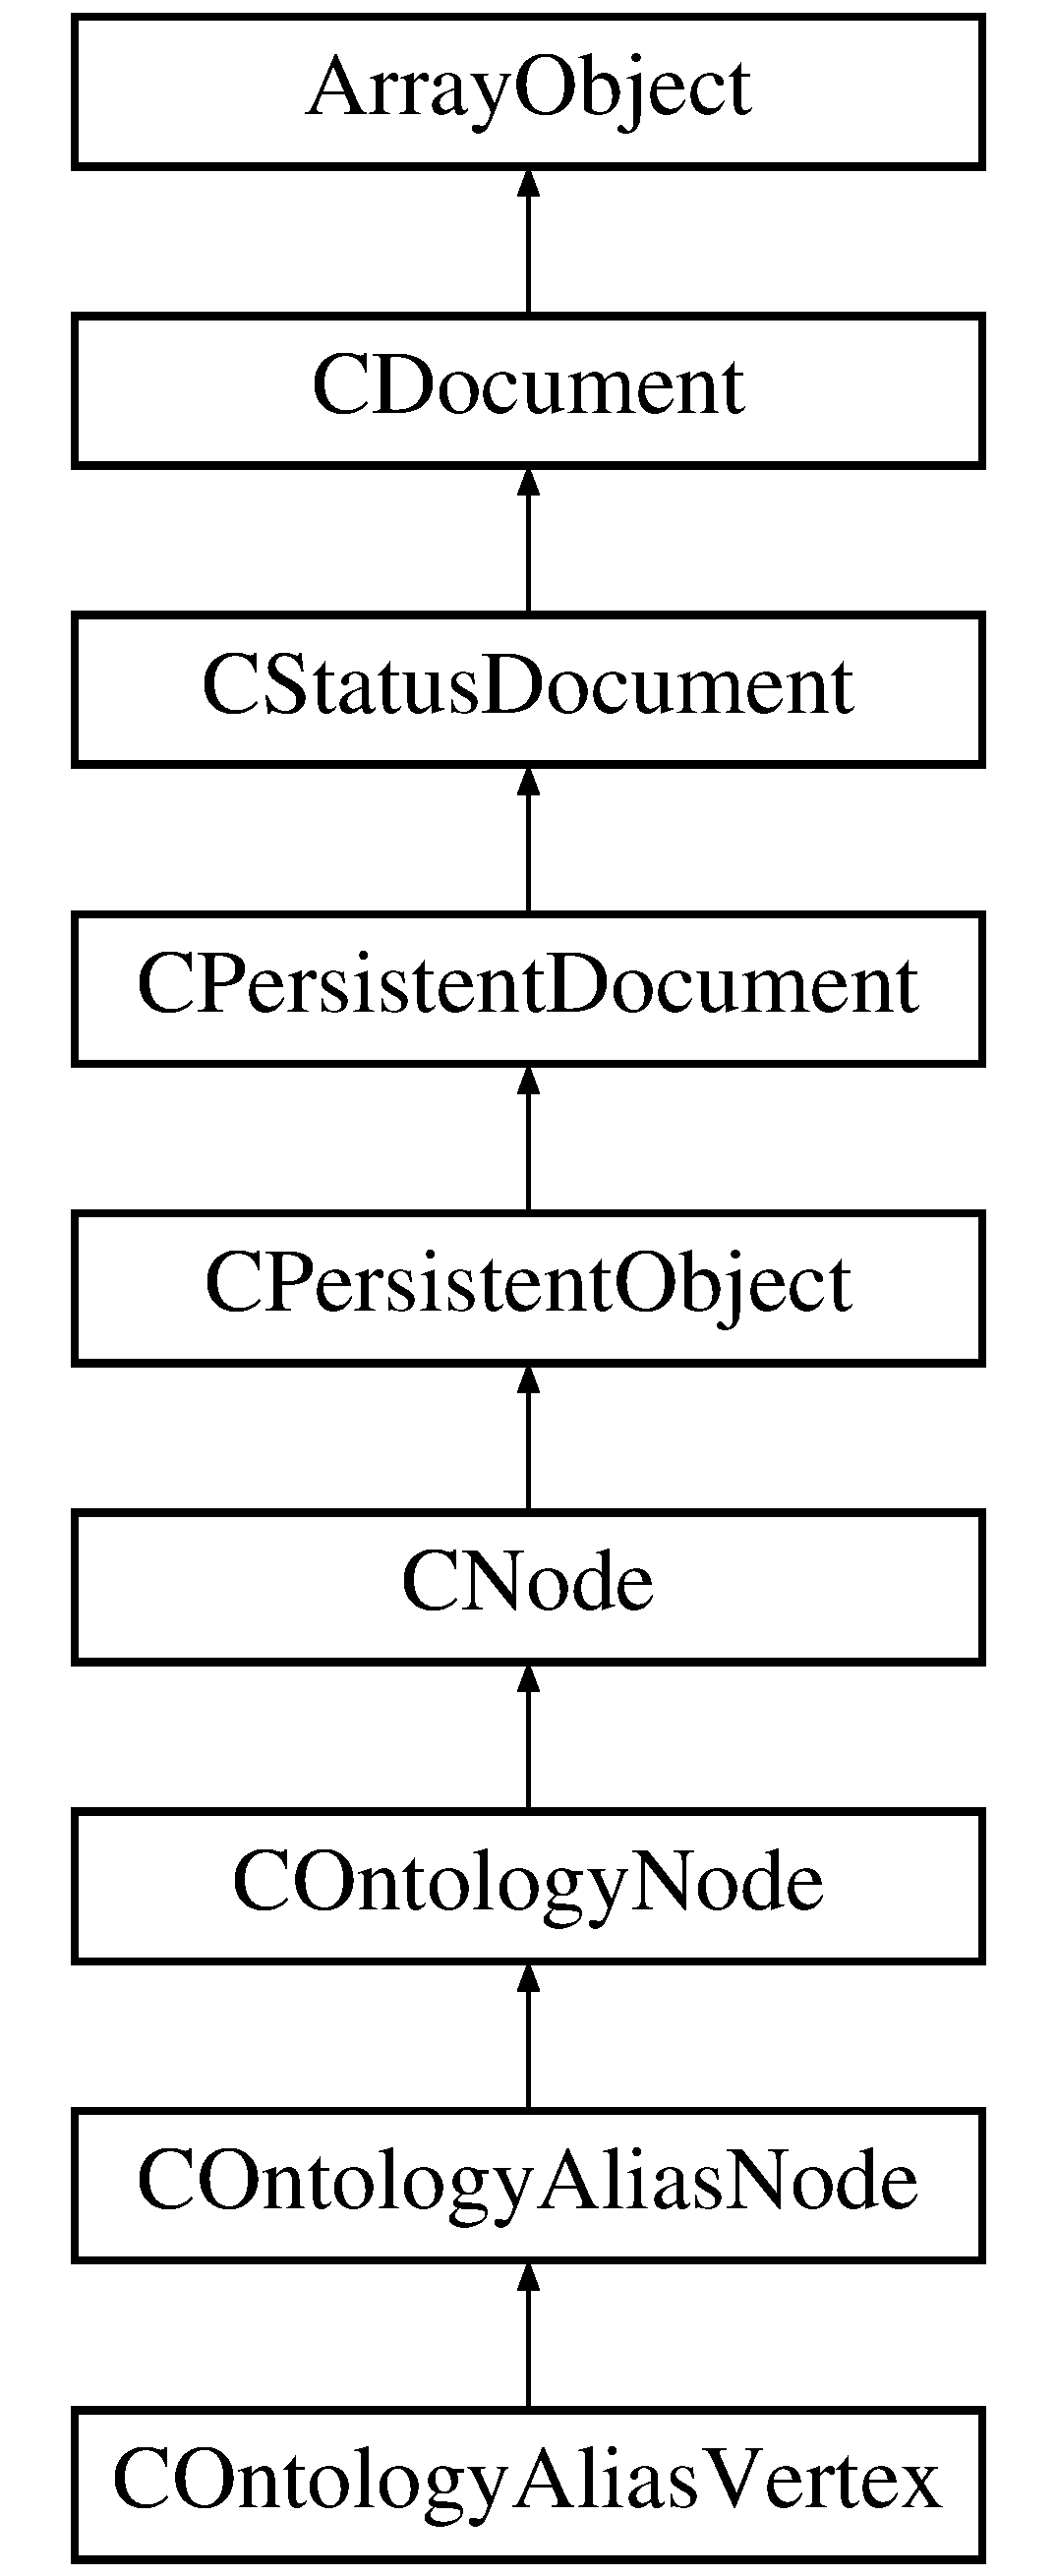
\includegraphics[height=9.000000cm]{class_c_ontology_alias_node}
\end{center}
\end{figure}
\subsection*{Public Member Functions}
\begin{DoxyCompactItemize}
\item 
\hyperlink{class_c_ontology_alias_node_aa9943ab171608dd41a95e0defc71820d}{Node} (\$the\-Value=N\-U\-L\-L, \$get\-Old=F\-A\-L\-S\-E)
\item 
\hyperlink{class_c_ontology_alias_node_ad82cf36f485558265dc30ac195c326f1}{Relate\-To} (\$the\-Predicate, \$the\-Object, \$the\-Connection=N\-U\-L\-L, \$do\-Propagate=T\-R\-U\-E)
\end{DoxyCompactItemize}
\subsection*{Static Public Member Functions}
\begin{DoxyCompactItemize}
\item 
static \hyperlink{class_c_ontology_alias_node_a1c50632496dcfad67765d134409cb71d}{Resolve} (\hyperlink{class_c_connection}{C\-Connection} \$the\-Connection, \$the\-Identifier, \$do\-Throw=F\-A\-L\-S\-E)
\end{DoxyCompactItemize}
\subsection*{Protected Member Functions}
\begin{DoxyCompactItemize}
\item 
\hyperlink{class_c_ontology_alias_node_a4b6c569d7b99fe7d1f171e408f49f2e5}{\-\_\-\-Precommit\-Related} (\&\$the\-Connection, \&\$the\-Modifiers)
\item 
\hyperlink{class_c_ontology_alias_node_acac06e2787b3d74a6a627a13e57e7154}{\-\_\-\-Postcommit\-Related} (\&\$the\-Connection, \&\$the\-Modifiers)
\end{DoxyCompactItemize}
\subsection*{Additional Inherited Members}


\subsection{Member Function Documentation}
\hypertarget{class_c_ontology_alias_node_acac06e2787b3d74a6a627a13e57e7154}{\index{C\-Ontology\-Alias\-Node@{C\-Ontology\-Alias\-Node}!\-\_\-\-Postcommit\-Related@{\-\_\-\-Postcommit\-Related}}
\index{\-\_\-\-Postcommit\-Related@{\-\_\-\-Postcommit\-Related}!COntologyAliasNode@{C\-Ontology\-Alias\-Node}}
\subsubsection[{\-\_\-\-Postcommit\-Related}]{\setlength{\rightskip}{0pt plus 5cm}C\-Ontology\-Alias\-Node\-::\-\_\-\-Postcommit\-Related (
\begin{DoxyParamCaption}
\item[{\&}]{\$the\-Connection, }
\item[{\&}]{\$the\-Modifiers}
\end{DoxyParamCaption}
)\hspace{0.3cm}{\ttfamily [protected]}}}\label{class_c_ontology_alias_node_acac06e2787b3d74a6a627a13e57e7154}
\subparagraph*{Update related objects after committing}

In this class we handle referenced master nodes, \hyperlink{}{k\-T\-A\-G\-\_\-\-N\-O\-D\-E}\-: depending on the value of the \hyperlink{}{k\-S\-W\-I\-T\-C\-H\-\_\-k\-T\-A\-G\-\_\-\-A\-L\-I\-A\-S\-\_\-\-N\-O\-D\-E\-S} flag we do the following\-:


\begin{DoxyItemize}
\item {\ttfamily 0x2}\-: {\itshape Keep count of references}. This means that the \hyperlink{}{k\-T\-A\-G\-\_\-\-N\-O\-D\-E\-S} attribute of the master node referenced by the \hyperlink{}{k\-T\-A\-G\-\_\-\-N\-O\-D\-E} attribute will be incremented when the object is inserted, or decremented when deleted. 
\item {\ttfamily 0x3}\-: {\itshape Keep list of references}. This means that a reference to the current object will be added to the \hyperlink{}{k\-T\-A\-G\-\_\-\-N\-O\-D\-E\-S} attribute of the master node referenced by \hyperlink{}{k\-T\-A\-G\-\_\-\-N\-O\-D\-E} attribute of the current object when the latter is inserted, and removed when the object isdeleted. 
\item {\ttfamily 0x0} {\itshape or other}\-: {\itshape Don't handle this information}. This means that the \hyperlink{}{k\-T\-A\-G\-\_\-\-N\-O\-D\-E\-S} attribute will not be handled. 
\end{DoxyItemize}


\begin{DoxyParams}[1]{Parameters}
reference & {\em \&\$the\-Connection} & Server, database or container. \\
\hline
reference & {\em \&\$the\-Modifiers} & Commit options.\\
\hline
\end{DoxyParams}
protected

\hyperlink{class_c_status_document_ab7d96fd4588cf7d5432fc65a1d1fb076}{\-\_\-\-Is\-Committed()}  \-\_\-\-Reference\-In\-Node()

\begin{DoxySeeAlso}{See Also}
k\-F\-L\-A\-G\-\_\-\-P\-E\-R\-S\-I\-S\-T\-\_\-\-I\-N\-S\-E\-R\-T k\-F\-L\-A\-G\-\_\-\-P\-E\-R\-S\-I\-S\-T\-\_\-\-R\-E\-P\-L\-A\-C\-E 
\end{DoxySeeAlso}
\hypertarget{class_c_ontology_alias_node_a4b6c569d7b99fe7d1f171e408f49f2e5}{\index{C\-Ontology\-Alias\-Node@{C\-Ontology\-Alias\-Node}!\-\_\-\-Precommit\-Related@{\-\_\-\-Precommit\-Related}}
\index{\-\_\-\-Precommit\-Related@{\-\_\-\-Precommit\-Related}!COntologyAliasNode@{C\-Ontology\-Alias\-Node}}
\subsubsection[{\-\_\-\-Precommit\-Related}]{\setlength{\rightskip}{0pt plus 5cm}C\-Ontology\-Alias\-Node\-::\-\_\-\-Precommit\-Related (
\begin{DoxyParamCaption}
\item[{\&}]{\$the\-Connection, }
\item[{\&}]{\$the\-Modifiers}
\end{DoxyParamCaption}
)\hspace{0.3cm}{\ttfamily [protected]}}}\label{class_c_ontology_alias_node_a4b6c569d7b99fe7d1f171e408f49f2e5}
\subparagraph*{Handle embedded or related objects before committing}

In this class we handle the master node\-: we check whether a master node related to the same term exists, if that is the case we set the current node's \hyperlink{}{k\-T\-A\-G\-\_\-\-N\-O\-D\-E} attribute, if that is not the case, we instantiate and insert the master node before setting its identifier in the current object's \hyperlink{}{k\-T\-A\-G\-\_\-\-N\-O\-D\-E} attribute.

Note that we do the above only if the \hyperlink{}{k\-T\-A\-G\-\_\-\-N\-O\-D\-E} offset is not yet set.


\begin{DoxyParams}[1]{Parameters}
reference & {\em \&\$the\-Connection} & Server, database or container. \\
\hline
reference & {\em \&\$the\-Modifiers} & Commit options.\\
\hline
\end{DoxyParams}
protected \begin{DoxyReturn}{Returns}
mixed
\end{DoxyReturn}
\hyperlink{class_c_ontology_node_a09eb3d9d16775d7752fd7bf62dd93d74}{Load\-Term()}

\begin{DoxySeeAlso}{See Also}
k\-T\-A\-G\-\_\-\-T\-E\-R\-M 
\end{DoxySeeAlso}
\hypertarget{class_c_ontology_alias_node_aa9943ab171608dd41a95e0defc71820d}{\index{C\-Ontology\-Alias\-Node@{C\-Ontology\-Alias\-Node}!Node@{Node}}
\index{Node@{Node}!COntologyAliasNode@{C\-Ontology\-Alias\-Node}}
\subsubsection[{Node}]{\setlength{\rightskip}{0pt plus 5cm}C\-Ontology\-Alias\-Node\-::\-Node (
\begin{DoxyParamCaption}
\item[{}]{\$the\-Value = {\ttfamily NULL}, }
\item[{}]{\$get\-Old = {\ttfamily FALSE}}
\end{DoxyParamCaption}
)}}\label{class_c_ontology_alias_node_aa9943ab171608dd41a95e0defc71820d}
\subparagraph*{Manage node reference}

This method can be used to manage the master node reference, \hyperlink{}{k\-T\-A\-G\-\_\-\-N\-O\-D\-E}, the method accepts a parameter which represents either the node, or the requested operation, depending on its value\-:


\begin{DoxyItemize}
\item {\ttfamily N\-U\-L\-L}\-: Return the current value. 
\item {\ttfamily F\-A\-L\-S\-E}\-: Delete the current value. 
\item {\itshape other}\-: Set the value with the provided parameter\-: 
\begin{DoxyItemize}
\item {\ttfamily integer}\-: This value will be interpreted as the node reference. 
\item {\ttfamily \hyperlink{class_c_ontology_node}{C\-Ontology\-Node}}\-: This value will be interpreted as the node object. 
\item {\itshape other}\-: Any other value will raise an exception. 
\end{DoxyItemize}
\end{DoxyItemize}

The second parameter is a boolean which if {\ttfamily T\-R\-U\-E} will return the {\itshape old} value when replacing containers; if {\ttfamily F\-A\-L\-S\-E}, it will return the currently set value.


\begin{DoxyParams}[1]{Parameters}
mixed & {\em \$the\-Value} & Term or operation. \\
\hline
boolean & {\em \$get\-Old} & {\ttfamily T\-R\-U\-E} get old value.\\
\hline
\end{DoxyParams}
public \begin{DoxyReturn}{Returns}
mixed {\itshape New} or {\itshape old} native container.
\end{DoxyReturn}
Manage\-Offset()

\begin{DoxySeeAlso}{See Also}
k\-T\-A\-G\-\_\-\-N\-O\-D\-E 
\end{DoxySeeAlso}
\hypertarget{class_c_ontology_alias_node_ad82cf36f485558265dc30ac195c326f1}{\index{C\-Ontology\-Alias\-Node@{C\-Ontology\-Alias\-Node}!Relate\-To@{Relate\-To}}
\index{Relate\-To@{Relate\-To}!COntologyAliasNode@{C\-Ontology\-Alias\-Node}}
\subsubsection[{Relate\-To}]{\setlength{\rightskip}{0pt plus 5cm}C\-Ontology\-Alias\-Node\-::\-Relate\-To (
\begin{DoxyParamCaption}
\item[{}]{\$the\-Predicate, }
\item[{}]{\$the\-Object, }
\item[{}]{\$the\-Connection = {\ttfamily NULL}, }
\item[{}]{\$do\-Propagate = {\ttfamily TRUE}}
\end{DoxyParamCaption}
)}}\label{class_c_ontology_alias_node_ad82cf36f485558265dc30ac195c326f1}
\subparagraph*{Relate to node}

We overload this method to mirror relationships between alias nodes to their counterpart master nodes, this is governed by the {\ttfamily \$do\-Propagate} switch.

We first create the requested relationship, then we resolve both the subject and the object, if it is also an alias, and we relate them with the same predicate.

This means that\-:


\begin{DoxyItemize}
\item {\itshape A\-L\-I\-A\-S =$>$ M\-A\-S\-T\-E\-R}\-: 
\begin{DoxyItemize}
\item A\-L\-I\-A\-S =$>$ M\-A\-S\-T\-E\-R 
\item A\-L\-I\-A\-S.\-M\-A\-S\-T\-E\-R =$>$ M\-A\-S\-T\-E\-R 
\end{DoxyItemize}
\item {\itshape A\-L\-I\-A\-S =$>$ A\-L\-I\-A\-S}\-: 
\begin{DoxyItemize}
\item A\-L\-I\-A\-S =$>$ A\-L\-I\-A\-S 
\item A\-L\-I\-A\-S.\-M\-A\-S\-T\-E\-R =$>$ A\-L\-I\-A\-S.\-M\-A\-S\-T\-E\-R 
\end{DoxyItemize}
\end{DoxyItemize}

We require the connection parameter here since both subject and object vertices must be committed by this method, this implies that the edge will also be committed.


\begin{DoxyParams}[1]{Parameters}
mixed & {\em \$the\-Predicate} & Predicate term object or reference. \\
\hline
mixed & {\em \$the\-Object} & Object node object or reference. \\
\hline
\hyperlink{class_c_connection}{C\-Connection} & {\em \$the\-Connection} & Server, database or container. \\
\hline
boolean & {\em \$do\-Propagate} & T\-R\-U\-E means relate masters.\\
\hline
\end{DoxyParams}
public \begin{DoxyReturn}{Returns}
\hyperlink{class_c_ontology_edge}{C\-Ontology\-Edge} Edge object. 
\end{DoxyReturn}
\hypertarget{class_c_ontology_alias_node_a1c50632496dcfad67765d134409cb71d}{\index{C\-Ontology\-Alias\-Node@{C\-Ontology\-Alias\-Node}!Resolve@{Resolve}}
\index{Resolve@{Resolve}!COntologyAliasNode@{C\-Ontology\-Alias\-Node}}
\subsubsection[{Resolve}]{\setlength{\rightskip}{0pt plus 5cm}static C\-Ontology\-Alias\-Node\-::\-Resolve (
\begin{DoxyParamCaption}
\item[{{\bf C\-Connection}}]{\$the\-Connection, }
\item[{}]{\$the\-Identifier, }
\item[{}]{\$do\-Throw = {\ttfamily FALSE}}
\end{DoxyParamCaption}
)\hspace{0.3cm}{\ttfamily [static]}}}\label{class_c_ontology_alias_node_a1c50632496dcfad67765d134409cb71d}
\subparagraph*{Resolve a node}

In this class we add the persistent identifier, \hyperlink{}{k\-T\-A\-G\-\_\-\-P\-I\-D}, to the list of properties to be checked, with this option we return the first match by default.


\begin{DoxyParams}[1]{Parameters}
\hyperlink{class_c_connection}{C\-Connection} & {\em \$the\-Connection} & Server, database or container. \\
\hline
mixed & {\em \$the\-Identifier} & Node identifier or term reference. \\
\hline
boolean & {\em \$do\-Throw} & If {\ttfamily T\-R\-U\-E} raise an exception.\\
\hline
\end{DoxyParams}
\begin{DoxyReturn}{Returns}
\hyperlink{class_c_ontology_node}{C\-Ontology\-Node} Matched node, found nodes or {\ttfamily N\-U\-L\-L}.
\end{DoxyReturn}

\begin{DoxyExceptions}{Exceptions}
{\em Exception} & \\
\hline
\end{DoxyExceptions}


The documentation for this class was generated from the following file\-:\begin{DoxyCompactItemize}
\item 
/\-Library/\-Web\-Server/\-Library/\-P\-H\-P\-Wrapper/classes/C\-Ontology\-Alias\-Node.\-php\end{DoxyCompactItemize}

\hypertarget{class_c_ontology_alias_vertex}{\section{C\-Ontology\-Alias\-Vertex Class Reference}
\label{class_c_ontology_alias_vertex}\index{C\-Ontology\-Alias\-Vertex@{C\-Ontology\-Alias\-Vertex}}
}
Inheritance diagram for C\-Ontology\-Alias\-Vertex\-:\begin{figure}[H]
\begin{center}
\leavevmode
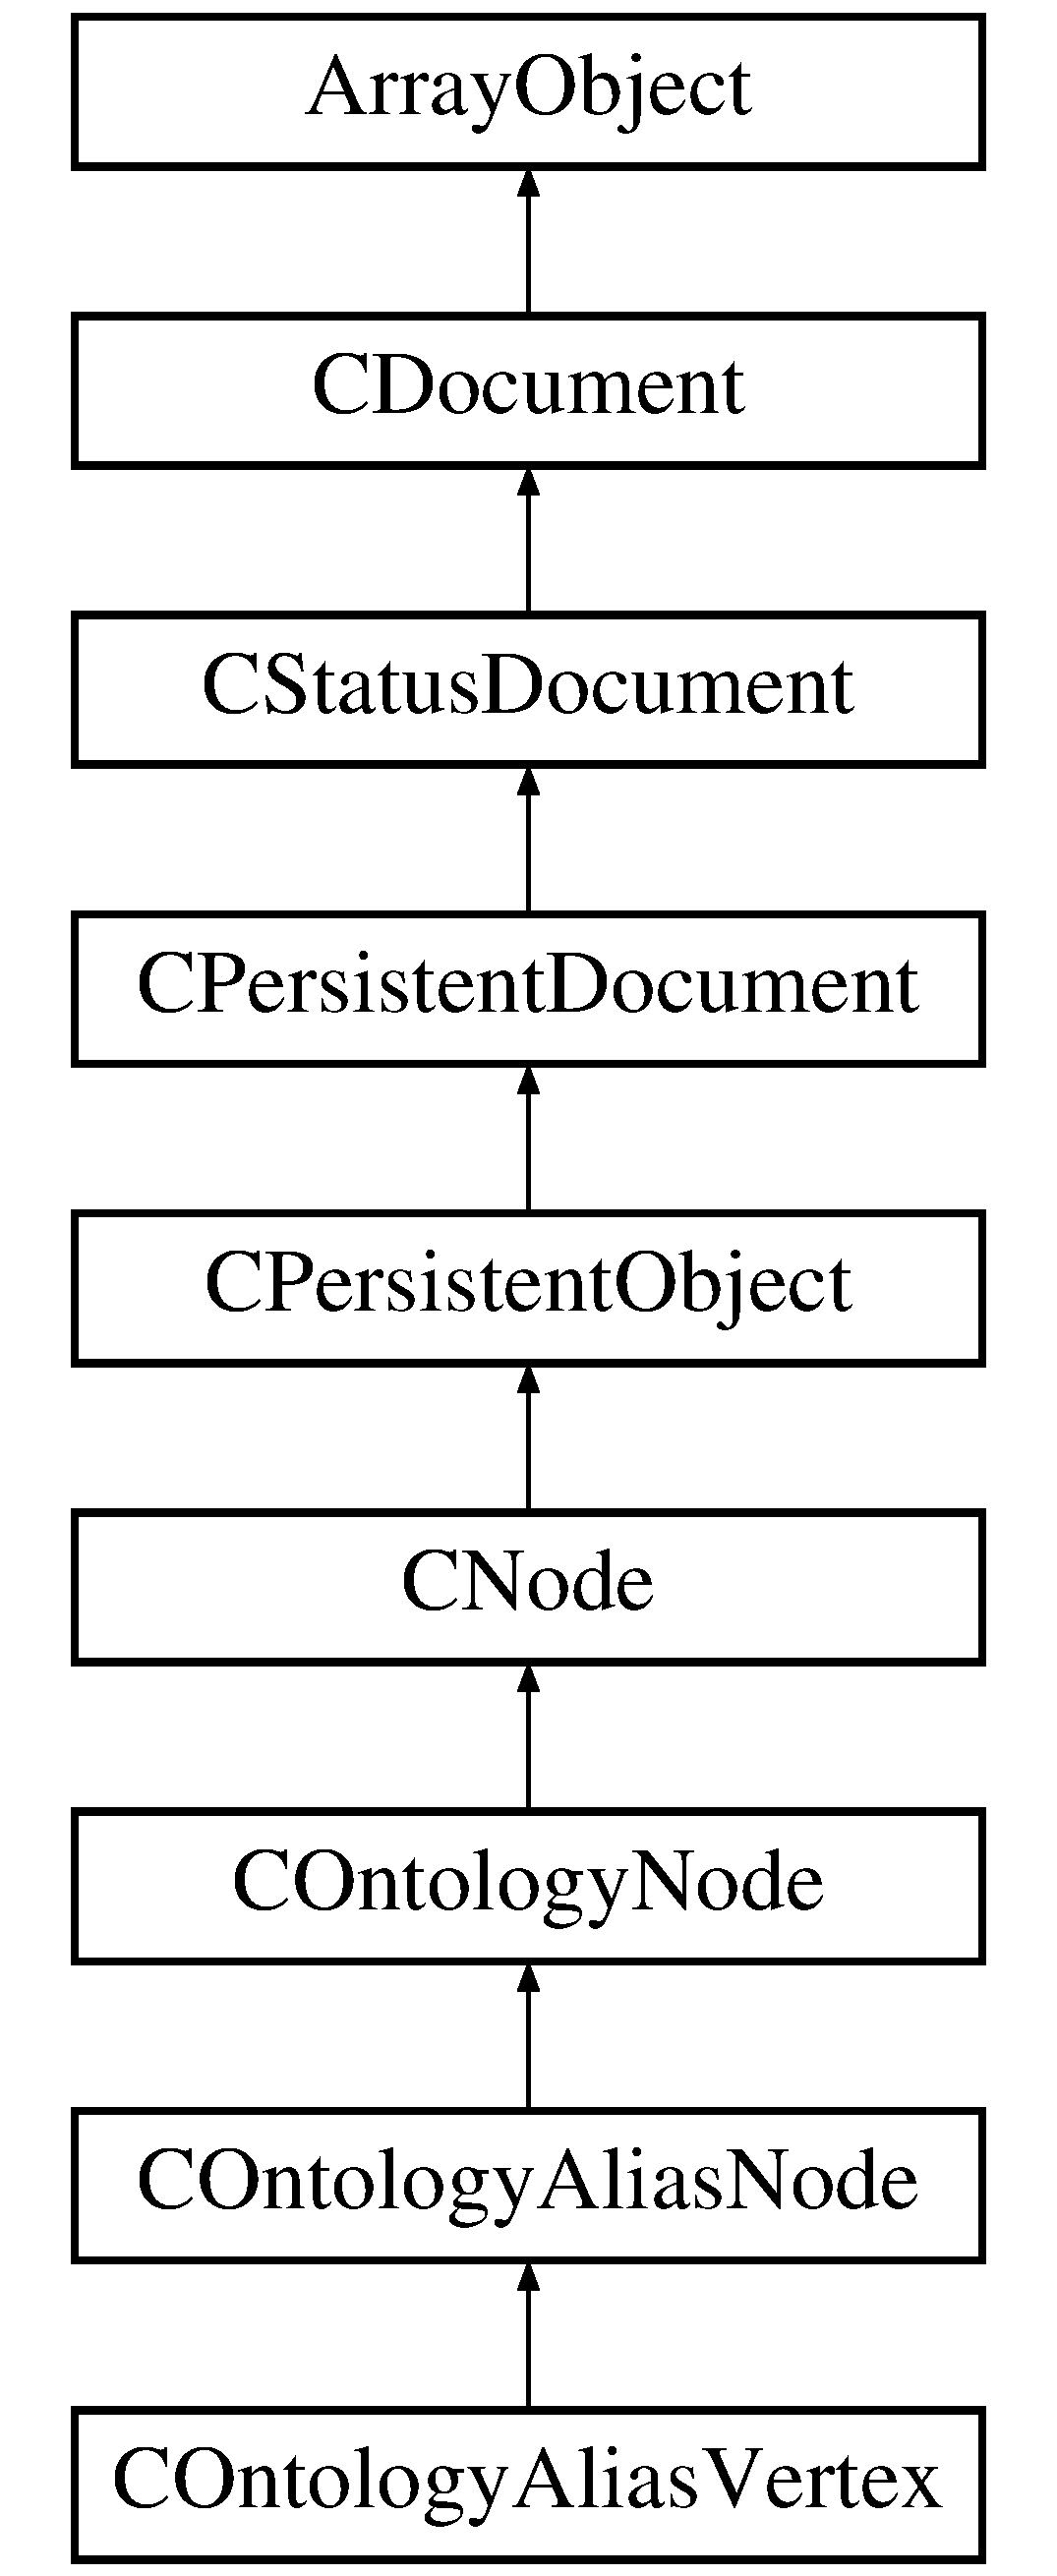
\includegraphics[height=9.000000cm]{class_c_ontology_alias_vertex}
\end{center}
\end{figure}
\subsection*{Protected Member Functions}
\begin{DoxyCompactItemize}
\item 
\hyperlink{class_c_ontology_alias_vertex_ae9bc78a01ea4f6f4adfa4fc5a9906adf}{\-\_\-\-Term\-Attributes} ()
\end{DoxyCompactItemize}
\subsection*{Additional Inherited Members}


\subsection{Member Function Documentation}
\hypertarget{class_c_ontology_alias_vertex_ae9bc78a01ea4f6f4adfa4fc5a9906adf}{\index{C\-Ontology\-Alias\-Vertex@{C\-Ontology\-Alias\-Vertex}!\-\_\-\-Term\-Attributes@{\-\_\-\-Term\-Attributes}}
\index{\-\_\-\-Term\-Attributes@{\-\_\-\-Term\-Attributes}!COntologyAliasVertex@{C\-Ontology\-Alias\-Vertex}}
\subsubsection[{\-\_\-\-Term\-Attributes}]{\setlength{\rightskip}{0pt plus 5cm}C\-Ontology\-Alias\-Vertex\-::\-\_\-\-Term\-Attributes (
\begin{DoxyParamCaption}
{}
\end{DoxyParamCaption}
)\hspace{0.3cm}{\ttfamily [protected]}}}\label{class_c_ontology_alias_vertex_ae9bc78a01ea4f6f4adfa4fc5a9906adf}
\subparagraph*{List term attributes}

In this class we return\-:


\begin{DoxyItemize}
\item {\ttfamily \hyperlink{}{k\-T\-A\-G\-\_\-\-L\-I\-D}}\-: The local identifier. 
\item {\ttfamily \hyperlink{}{k\-T\-A\-G\-\_\-\-G\-I\-D}}\-: The global identifier. 
\item {\ttfamily \hyperlink{}{k\-T\-A\-G\-\_\-\-L\-A\-B\-E\-L}}\-: The label. 
\item {\ttfamily \hyperlink{}{k\-T\-A\-G\-\_\-\-D\-E\-F\-I\-N\-I\-T\-I\-O\-N}}\-: The definition. 
\item {\ttfamily \hyperlink{}{k\-T\-A\-G\-\_\-\-F\-E\-A\-T\-U\-R\-E\-S}}\-: The feature tag references. 
\item {\ttfamily \hyperlink{}{k\-T\-A\-G\-\_\-\-S\-C\-A\-L\-E\-S}}\-: The scale tag references. 
\end{DoxyItemize}

protected \begin{DoxyReturn}{Returns}
array 
\end{DoxyReturn}


The documentation for this class was generated from the following file\-:\begin{DoxyCompactItemize}
\item 
/\-Library/\-Web\-Server/\-Library/\-P\-H\-P\-Wrapper/classes/C\-Ontology\-Alias\-Vertex.\-php\end{DoxyCompactItemize}

\hypertarget{class_c_ontology_edge}{\section{C\-Ontology\-Edge Class Reference}
\label{class_c_ontology_edge}\index{C\-Ontology\-Edge@{C\-Ontology\-Edge}}
}
Inheritance diagram for C\-Ontology\-Edge\-:\begin{figure}[H]
\begin{center}
\leavevmode
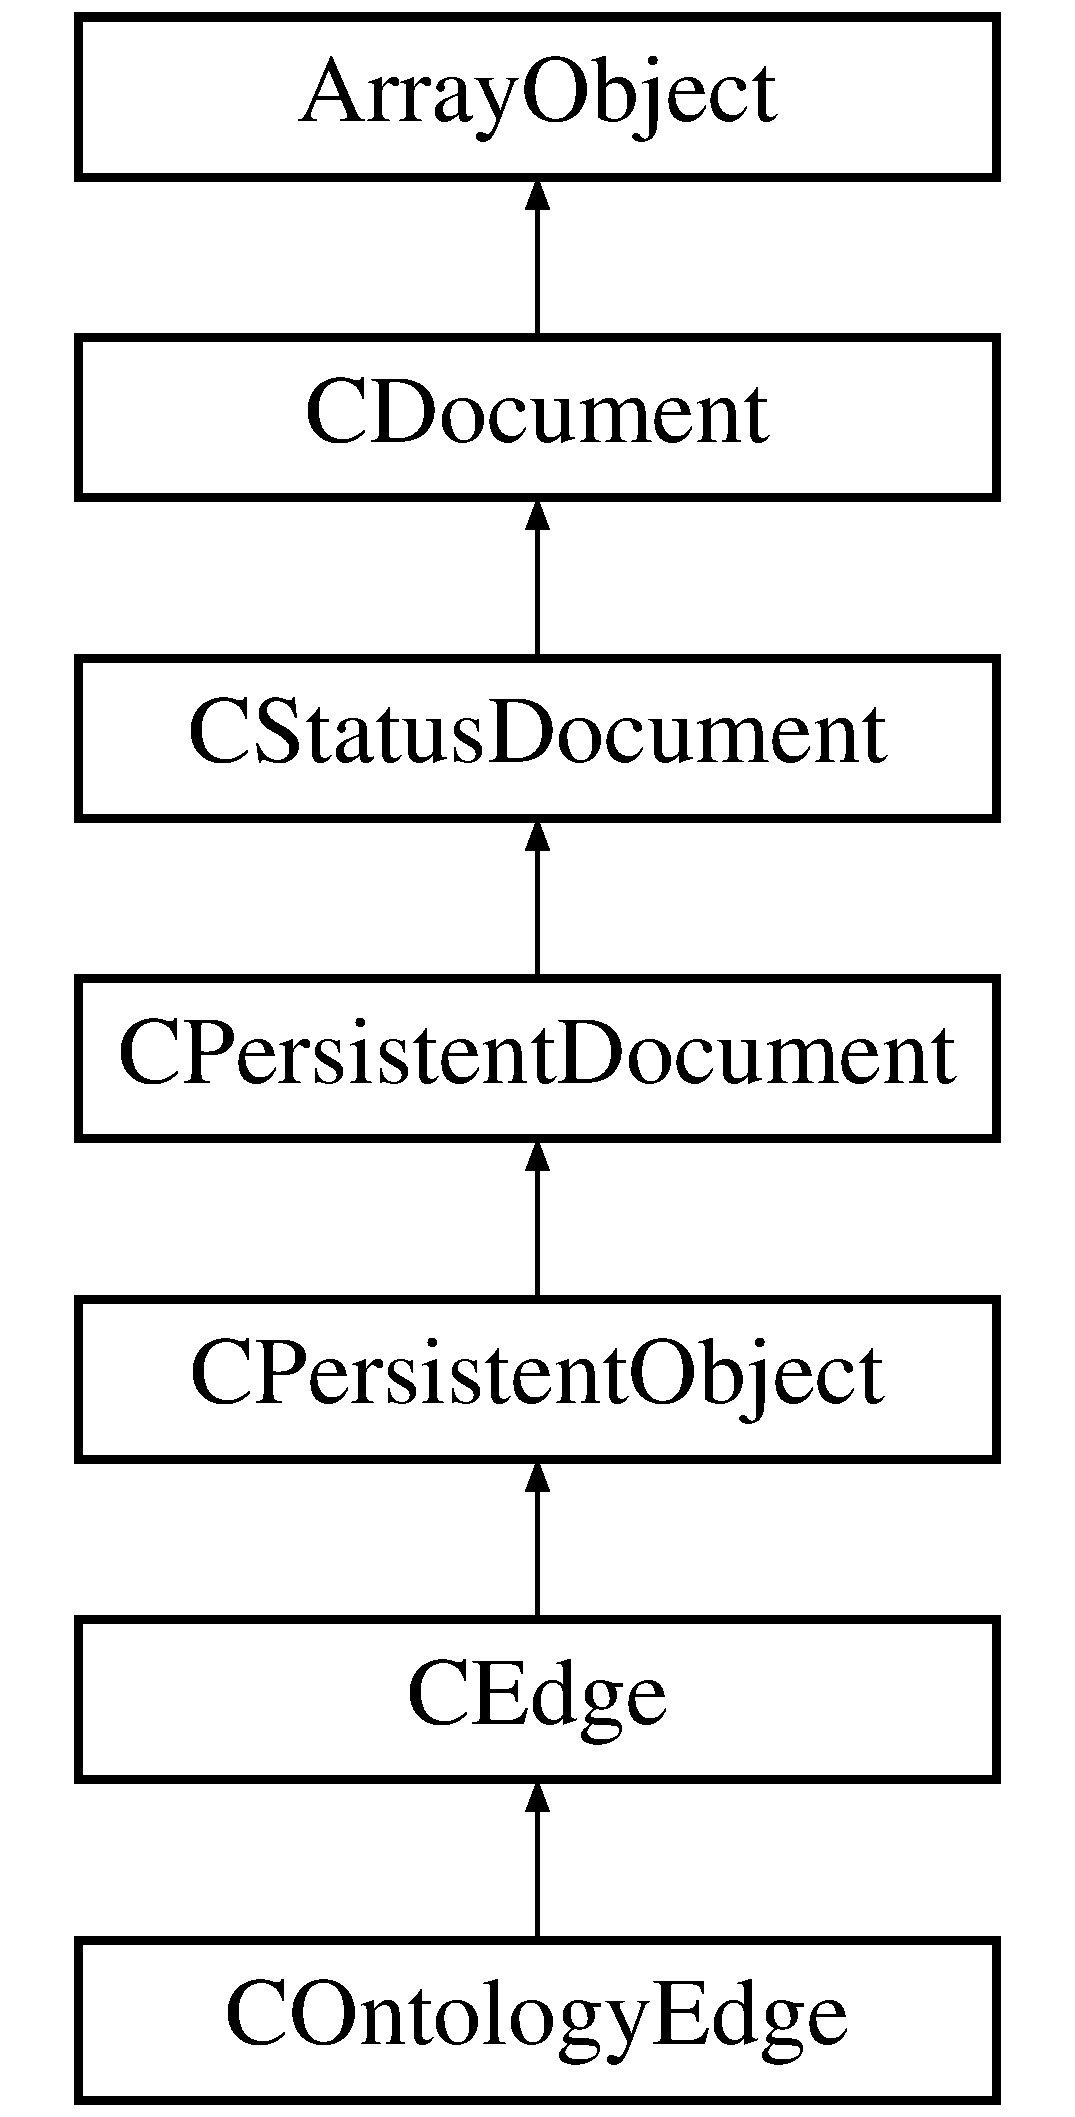
\includegraphics[height=7.000000cm]{class_c_ontology_edge}
\end{center}
\end{figure}
\subsection*{Public Member Functions}
\begin{DoxyCompactItemize}
\item 
\hyperlink{class_c_ontology_edge_accb7245cafff2b1f86e5ef54f0b350b8}{Insert} (\hyperlink{class_c_connection}{C\-Connection} \$the\-Connection)
\item 
\hyperlink{class_c_ontology_edge_a0f369a60b57a48e79c34537a1ec6de80}{Load\-Subject} (\hyperlink{class_c_connection}{C\-Connection} \$the\-Connection, \$do\-Reload=F\-A\-L\-S\-E)
\item 
\hyperlink{class_c_ontology_edge_a74b5faea0ec803afd1c44e739b588b63}{Load\-Predicate} (\hyperlink{class_c_connection}{C\-Connection} \$the\-Connection, \$do\-Reload=F\-A\-L\-S\-E)
\item 
\hyperlink{class_c_ontology_edge_aff6fa3df789a8915076b07062e45bec2}{Load\-Object} (\hyperlink{class_c_connection}{C\-Connection} \$the\-Connection, \$do\-Reload=F\-A\-L\-S\-E)
\end{DoxyCompactItemize}
\subsection*{Static Public Member Functions}
\begin{DoxyCompactItemize}
\item 
static \hyperlink{class_c_ontology_edge_affe02c782c1cc05ea2949cbd48b07c54}{Default\-Container\-Name} ()
\item 
static \hyperlink{class_c_ontology_edge_ad9312fa22db2de8a45f9dc5cdce204ed}{Resolve} (\hyperlink{class_c_connection}{C\-Connection} \$the\-Connection, \$the\-Identifier, \$do\-Throw=F\-A\-L\-S\-E)
\end{DoxyCompactItemize}
\subsection*{Protected Member Functions}
\begin{DoxyCompactItemize}
\item 
\hyperlink{class_c_ontology_edge_a8e5d17a08008ca21f0be3ffd801890ef}{\-\_\-index} (\hyperlink{class_c_connection}{C\-Connection} \$the\-Connection, \$the\-Modifiers)
\item 
\hyperlink{class_c_ontology_edge_a001291e06296d03d90254b063581b3f9}{\-\_\-\-Preset} (\&\$the\-Offset, \&\$the\-Value)
\item 
\hyperlink{class_c_ontology_edge_adfb3c6b7fe4fd70f465a225ebb605565}{\-\_\-\-Preunset} (\&\$the\-Offset)
\item 
\hyperlink{class_c_ontology_edge_ad014041738697d960791d7ee489dcc26}{\-\_\-\-Precommit\-Related} (\&\$the\-Connection, \&\$the\-Modifiers)
\item 
\hyperlink{class_c_ontology_edge_ac76cb6503b256fa7f6599a1cd98ab5cd}{\-\_\-\-Precommit\-Identify} (\&\$the\-Connection, \&\$the\-Modifiers)
\item 
\hyperlink{class_c_ontology_edge_a489c9ec3268156e7bef68eccec679fa5}{\-\_\-\-Postcommit\-Related} (\&\$the\-Connection, \&\$the\-Modifiers)
\item 
\hyperlink{class_c_ontology_edge_a416c0d2e9e040ae28b1cf05ff6bbd947}{\-\_\-\-Postcommit\-Cleanup} (\&\$the\-Connection, \&\$the\-Modifiers)
\item 
\hyperlink{class_c_ontology_edge_acc6425bab1f7e9988b1be0cfc977533e}{\-\_\-\-Add\-Graph\-Edge} (\hyperlink{class_c_graph_container}{C\-Graph\-Container} \$the\-Graph)
\end{DoxyCompactItemize}
\subsection*{Protected Attributes}
\begin{DoxyCompactItemize}
\item 
\hypertarget{class_c_ontology_edge_a6b69e9b2597ea1ca7d07dd54e2c40ae2}{{\bfseries \$m\-Subject} = N\-U\-L\-L}\label{class_c_ontology_edge_a6b69e9b2597ea1ca7d07dd54e2c40ae2}

\item 
\hypertarget{class_c_ontology_edge_a8b596151b0cf3a60aad60bc1e7cfec7d}{{\bfseries \$m\-Predicate} = N\-U\-L\-L}\label{class_c_ontology_edge_a8b596151b0cf3a60aad60bc1e7cfec7d}

\item 
\hypertarget{class_c_ontology_edge_a3ba70a64095979da7533fb6124ec49b7}{{\bfseries \$m\-Object} = N\-U\-L\-L}\label{class_c_ontology_edge_a3ba70a64095979da7533fb6124ec49b7}

\end{DoxyCompactItemize}


\subsection{Member Function Documentation}
\hypertarget{class_c_ontology_edge_acc6425bab1f7e9988b1be0cfc977533e}{\index{C\-Ontology\-Edge@{C\-Ontology\-Edge}!\-\_\-\-Add\-Graph\-Edge@{\-\_\-\-Add\-Graph\-Edge}}
\index{\-\_\-\-Add\-Graph\-Edge@{\-\_\-\-Add\-Graph\-Edge}!COntologyEdge@{C\-Ontology\-Edge}}
\subsubsection[{\-\_\-\-Add\-Graph\-Edge}]{\setlength{\rightskip}{0pt plus 5cm}C\-Ontology\-Edge\-::\-\_\-\-Add\-Graph\-Edge (
\begin{DoxyParamCaption}
\item[{{\bf C\-Graph\-Container}}]{\$the\-Graph}
\end{DoxyParamCaption}
)\hspace{0.3cm}{\ttfamily [protected]}}}\label{class_c_ontology_edge_acc6425bab1f7e9988b1be0cfc977533e}
\subparagraph*{Create graph edge}

This method will create and save a new graph edge in the provided graph container and return its newly created identifier.

This method is called by \hyperlink{class_c_ontology_edge_ac76cb6503b256fa7f6599a1cd98ab5cd}{\-\_\-\-Precommit\-Identify()} to set the new edge \hyperlink{}{k\-T\-A\-G\-\_\-\-N\-I\-D} and the method makes no assumption whether the edge exists already or not, in all cases it will create a new edge.

This method will set the node identifiers in the \hyperlink{}{k\-T\-A\-G\-\_\-\-S\-U\-B\-J\-E\-C\-T} and \hyperlink{}{k\-T\-A\-G\-\_\-\-O\-B\-J\-E\-C\-T} properties and the predicate term \hyperlink{}{k\-T\-A\-G\-\_\-\-G\-I\-D} as the predicate identifier.

following attributes to the graph edge\-: \hyperlink{}{k\-T\-A\-G\-\_\-\-K\-I\-N\-D} and \hyperlink{}{k\-T\-A\-G\-\_\-\-T\-Y\-P\-E}, derived classes may override this method to add other properties.

The method should raise an exception if the node was not created.


\begin{DoxyParams}[1]{Parameters}
\hyperlink{class_c_graph_container}{C\-Graph\-Container} & {\em \$the\-Graph} & Graph container.\\
\hline
\end{DoxyParams}
protected \begin{DoxyReturn}{Returns}
integer Newly created edge I\-D. 
\end{DoxyReturn}
\hypertarget{class_c_ontology_edge_a8e5d17a08008ca21f0be3ffd801890ef}{\index{C\-Ontology\-Edge@{C\-Ontology\-Edge}!\-\_\-index@{\-\_\-index}}
\index{\-\_\-index@{\-\_\-index}!COntologyEdge@{C\-Ontology\-Edge}}
\subsubsection[{\-\_\-index}]{\setlength{\rightskip}{0pt plus 5cm}C\-Ontology\-Edge\-::\-\_\-index (
\begin{DoxyParamCaption}
\item[{{\bf C\-Connection}}]{\$the\-Connection, }
\item[{}]{\$the\-Modifiers}
\end{DoxyParamCaption}
)\hspace{0.3cm}{\ttfamily [protected]}}}\label{class_c_ontology_edge_a8e5d17a08008ca21f0be3ffd801890ef}
\subparagraph*{Return the object's global unique identifier}

We override the parent method to handle the referenced objects\-: in this class the global identifier is the concatenation of the subject node native identifier, the predicate global identifier and the object node native identifier all separated by the \hyperlink{}{k\-T\-O\-K\-E\-N\-\_\-\-I\-N\-D\-E\-X\-\_\-\-S\-E\-P\-A\-R\-A\-T\-O\-R} token.

This method will also automatically fill the persistent path, \hyperlink{}{k\-T\-A\-G\-\_\-\-P\-A\-T\-H}, and identifier, \hyperlink{}{k\-T\-A\-G\-\_\-\-P\-I\-D}, in which the vertex node identifiers are replaced by their related term global identifiers. These attributes are useful for debugging purposes and to provide a persistent identifier to the edge.


\begin{DoxyParams}[1]{Parameters}
\hyperlink{class_c_connection}{C\-Connection} & {\em \$the\-Connection} & Server, database or container. \\
\hline
bitfield & {\em \$the\-Modifiers} & Commit options.\\
\hline
\end{DoxyParams}

\begin{DoxyExceptions}{Exceptions}
{\em Exception} & protected \\
\hline
\end{DoxyExceptions}
\begin{DoxyReturn}{Returns}
string$|$\-N\-U\-L\-L The object's global unique identifier.
\end{DoxyReturn}

\begin{DoxyExceptions}{Exceptions}
{\em Exception} & \hyperlink{class_c_ontology_edge_a0f369a60b57a48e79c34537a1ec6de80}{Load\-Subject()}  \hyperlink{class_c_ontology_edge_a74b5faea0ec803afd1c44e739b588b63}{Load\-Predicate()}  \hyperlink{class_c_ontology_edge_aff6fa3df789a8915076b07062e45bec2}{Load\-Object()}\\
\hline
\end{DoxyExceptions}
\begin{DoxySeeAlso}{See Also}
k\-T\-A\-G\-\_\-\-N\-I\-D k\-T\-A\-G\-\_\-\-G\-I\-D k\-T\-A\-G\-\_\-\-P\-I\-D k\-T\-A\-G\-\_\-\-P\-A\-T\-H k\-T\-O\-K\-E\-N\-\_\-\-I\-N\-D\-E\-X\-\_\-\-S\-E\-P\-A\-R\-A\-T\-O\-R 
\end{DoxySeeAlso}
\hypertarget{class_c_ontology_edge_a416c0d2e9e040ae28b1cf05ff6bbd947}{\index{C\-Ontology\-Edge@{C\-Ontology\-Edge}!\-\_\-\-Postcommit\-Cleanup@{\-\_\-\-Postcommit\-Cleanup}}
\index{\-\_\-\-Postcommit\-Cleanup@{\-\_\-\-Postcommit\-Cleanup}!COntologyEdge@{C\-Ontology\-Edge}}
\subsubsection[{\-\_\-\-Postcommit\-Cleanup}]{\setlength{\rightskip}{0pt plus 5cm}C\-Ontology\-Edge\-::\-\_\-\-Postcommit\-Cleanup (
\begin{DoxyParamCaption}
\item[{\&}]{\$the\-Connection, }
\item[{\&}]{\$the\-Modifiers}
\end{DoxyParamCaption}
)\hspace{0.3cm}{\ttfamily [protected]}}}\label{class_c_ontology_edge_a416c0d2e9e040ae28b1cf05ff6bbd947}
\subparagraph*{Cleanup the object after committing}

In this class we reset the term object cache, we set the data members to {\ttfamily N\-U\-L\-L} so that next time one wants to retrieve related objects, the cache will have to be refreshed.


\begin{DoxyParams}[1]{Parameters}
reference & {\em \&\$the\-Connection} & Server, database or container. \\
\hline
reference & {\em \&\$the\-Modifiers} & Commit options.\\
\hline
\end{DoxyParams}
protected \hypertarget{class_c_ontology_edge_a489c9ec3268156e7bef68eccec679fa5}{\index{C\-Ontology\-Edge@{C\-Ontology\-Edge}!\-\_\-\-Postcommit\-Related@{\-\_\-\-Postcommit\-Related}}
\index{\-\_\-\-Postcommit\-Related@{\-\_\-\-Postcommit\-Related}!COntologyEdge@{C\-Ontology\-Edge}}
\subsubsection[{\-\_\-\-Postcommit\-Related}]{\setlength{\rightskip}{0pt plus 5cm}C\-Ontology\-Edge\-::\-\_\-\-Postcommit\-Related (
\begin{DoxyParamCaption}
\item[{\&}]{\$the\-Connection, }
\item[{\&}]{\$the\-Modifiers}
\end{DoxyParamCaption}
)\hspace{0.3cm}{\ttfamily [protected]}}}\label{class_c_ontology_edge_a489c9ec3268156e7bef68eccec679fa5}
\subparagraph*{Update related objects after committing}

In this class we handle the \hyperlink{}{k\-T\-A\-G\-\_\-\-E\-D\-G\-E\-S} attribute of the nodes referenced by this object depending on the value of the \hyperlink{}{k\-S\-W\-I\-T\-C\-H\-\_\-k\-T\-A\-G\-\_\-\-E\-D\-G\-E\-S} flag we do the following\-:


\begin{DoxyItemize}
\item {\ttfamily 0x2}\-: {\itshape Keep count of references}. This means that the \hyperlink{}{k\-T\-A\-G\-\_\-\-E\-D\-G\-E\-S} attribute of the subject or object nodes referenced by the current object will be incremented when the object is inserted, or decremented when deleted. 
\item {\ttfamily 0x3}\-: {\itshape Keep list of references}. This means that a reference to the current object will be added to the \hyperlink{}{k\-T\-A\-G\-\_\-\-E\-D\-G\-E\-S} attribute of the referenced subject or object nodes and removed when the object is deleted. 
\item {\ttfamily 0x0} {\itshape or other}\-: {\itshape Don't handle this information}. This means that the \hyperlink{}{k\-T\-A\-G\-\_\-\-E\-D\-G\-E\-S} attribute will not be handled. 
\end{DoxyItemize}

Note that you should provide either a database connection or the {\itshape node} container to this method in order to make it work!

This is the method that should take care of alias to master replication of the relationships, the code is commented\-: if you want to automatically relate alias's master nodes, uncomment that section of use the node's Relate\-To() method in which you can choose whether or not to relate masters.


\begin{DoxyParams}[1]{Parameters}
reference & {\em \&\$the\-Connection} & Server, database or container. \\
\hline
reference & {\em \&\$the\-Modifiers} & Commit options.\\
\hline
\end{DoxyParams}
protected

\hyperlink{class_c_status_document_ab7d96fd4588cf7d5432fc65a1d1fb076}{\-\_\-\-Is\-Committed()}  \hyperlink{class_c_persistent_object_ae5f9319ab169499181ae8db82b2fc0e7}{\-\_\-\-Reference\-In\-Object()}

\begin{DoxySeeAlso}{See Also}
k\-T\-A\-G\-\_\-\-E\-D\-G\-E\-S k\-T\-A\-G\-\_\-\-S\-U\-B\-J\-E\-C\-T k\-T\-A\-G\-\_\-\-O\-B\-J\-E\-C\-T 

k\-F\-L\-A\-G\-\_\-\-P\-E\-R\-S\-I\-S\-T\-\_\-\-I\-N\-S\-E\-R\-T k\-F\-L\-A\-G\-\_\-\-P\-E\-R\-S\-I\-S\-T\-\_\-\-R\-E\-P\-L\-A\-C\-E k\-F\-L\-A\-G\-\_\-\-P\-E\-R\-S\-I\-S\-T\-\_\-\-D\-E\-L\-E\-T\-E 

k\-F\-L\-A\-G\-\_\-\-P\-E\-R\-S\-I\-S\-T\-\_\-\-M\-O\-D\-I\-F\-Y k\-F\-L\-A\-G\-\_\-\-M\-O\-D\-I\-F\-Y\-\_\-\-A\-D\-D\-S\-E\-T k\-F\-L\-A\-G\-\_\-\-M\-O\-D\-I\-F\-Y\-\_\-\-P\-U\-L\-L 
\end{DoxySeeAlso}
\hypertarget{class_c_ontology_edge_ac76cb6503b256fa7f6599a1cd98ab5cd}{\index{C\-Ontology\-Edge@{C\-Ontology\-Edge}!\-\_\-\-Precommit\-Identify@{\-\_\-\-Precommit\-Identify}}
\index{\-\_\-\-Precommit\-Identify@{\-\_\-\-Precommit\-Identify}!COntologyEdge@{C\-Ontology\-Edge}}
\subsubsection[{\-\_\-\-Precommit\-Identify}]{\setlength{\rightskip}{0pt plus 5cm}C\-Ontology\-Edge\-::\-\_\-\-Precommit\-Identify (
\begin{DoxyParamCaption}
\item[{\&}]{\$the\-Connection, }
\item[{\&}]{\$the\-Modifiers}
\end{DoxyParamCaption}
)\hspace{0.3cm}{\ttfamily [protected]}}}\label{class_c_ontology_edge_ac76cb6503b256fa7f6599a1cd98ab5cd}
\subparagraph*{Determine the identifiers before committing}

This method will use the result of the \hyperlink{class_c_ontology_edge_a8e5d17a08008ca21f0be3ffd801890ef}{\-\_\-index()} method to set the global identifier, \hyperlink{}{k\-T\-A\-G\-\_\-\-G\-I\-D}; the same value will be hashed and constitute the unique identifier, \hyperlink{}{k\-T\-A\-G\-\_\-\-U\-I\-D}.

This method will also take care of generating the sequence number that represents the object's native identifier, \hyperlink{}{k\-T\-A\-G\-\_\-\-N\-I\-D}, this value can be generated in two ways\-:


\begin{DoxyItemize}
\item {\itshape The container has the graph reference, \hyperlink{}{k\-O\-F\-F\-S\-E\-T\-\_\-\-G\-R\-A\-P\-H}}\-: If the provided container contains a reference to a graph container, it means that the edge must also be stored in the graph, this will be taken care by the \hyperlink{class_c_ontology_edge_acc6425bab1f7e9988b1be0cfc977533e}{\-\_\-\-Add\-Graph\-Edge()} method that will return the graph edge's I\-D, which in turn will become the current object's \hyperlink{}{k\-T\-A\-G\-\_\-\-N\-I\-D}. 
\item {\itshape The container lacks the graph reference, \hyperlink{}{k\-O\-F\-F\-S\-E\-T\-\_\-\-G\-R\-A\-P\-H}}\-: If the provided container does not hold a reference to a graph container, the object identifier will be generated with a sequence number tagged \hyperlink{}{k\-S\-E\-Q\-U\-E\-N\-C\-E\-\_\-\-K\-E\-Y\-\_\-\-E\-D\-G\-E}, this method will set the native identifier, \hyperlink{}{k\-T\-A\-G\-\_\-\-N\-I\-D}, with this value. 
\end{DoxyItemize}

When deleting the object, if the provided container contains a reference to a graph container, this method will also delete the relative edge from the graph.

The parent method will then be called, which will ignore the global and native identifiers, since they will have been set here.


\begin{DoxyParams}[1]{Parameters}
reference & {\em \&\$the\-Connection} & Server, database or container. \\
\hline
reference & {\em \&\$the\-Modifiers} & Commit options.\\
\hline
\end{DoxyParams}
protected \begin{DoxyReturn}{Returns}
mixed
\end{DoxyReturn}

\begin{DoxyExceptions}{Exceptions}
{\em Exception} & \\
\hline
\end{DoxyExceptions}
\begin{DoxySeeAlso}{See Also}
k\-S\-E\-Q\-U\-E\-N\-C\-E\-\_\-\-K\-E\-Y\-\_\-\-E\-D\-G\-E 

k\-T\-A\-G\-\_\-\-N\-I\-D k\-T\-A\-G\-\_\-\-G\-I\-D k\-T\-A\-G\-\_\-\-U\-I\-D 

k\-F\-L\-A\-G\-\_\-\-P\-E\-R\-S\-I\-S\-T\-\_\-\-I\-N\-S\-E\-R\-T k\-F\-L\-A\-G\-\_\-\-P\-E\-R\-S\-I\-S\-T\-\_\-\-R\-E\-P\-L\-A\-C\-E 
\end{DoxySeeAlso}
\hypertarget{class_c_ontology_edge_ad014041738697d960791d7ee489dcc26}{\index{C\-Ontology\-Edge@{C\-Ontology\-Edge}!\-\_\-\-Precommit\-Related@{\-\_\-\-Precommit\-Related}}
\index{\-\_\-\-Precommit\-Related@{\-\_\-\-Precommit\-Related}!COntologyEdge@{C\-Ontology\-Edge}}
\subsubsection[{\-\_\-\-Precommit\-Related}]{\setlength{\rightskip}{0pt plus 5cm}C\-Ontology\-Edge\-::\-\_\-\-Precommit\-Related (
\begin{DoxyParamCaption}
\item[{\&}]{\$the\-Connection, }
\item[{\&}]{\$the\-Modifiers}
\end{DoxyParamCaption}
)\hspace{0.3cm}{\ttfamily [protected]}}}\label{class_c_ontology_edge_ad014041738697d960791d7ee489dcc26}
\subparagraph*{Handle embedded or related objects before committing}

In this class we commit the eventual term provided as an uncommitted object and replace the offset with the term's native identifier, or load the term if provided as an identifier.


\begin{DoxyParams}[1]{Parameters}
reference & {\em \&\$the\-Connection} & Server, database or container. \\
\hline
reference & {\em \&\$the\-Modifiers} & Commit options.\\
\hline
\end{DoxyParams}
protected \begin{DoxyReturn}{Returns}
mixed
\end{DoxyReturn}
\hyperlink{class_c_ontology_edge_a0f369a60b57a48e79c34537a1ec6de80}{Load\-Subject()}  \hyperlink{class_c_ontology_edge_a74b5faea0ec803afd1c44e739b588b63}{Load\-Predicate()}  \hyperlink{class_c_ontology_edge_aff6fa3df789a8915076b07062e45bec2}{Load\-Object()}

\begin{DoxySeeAlso}{See Also}
k\-T\-A\-G\-\_\-\-P\-R\-E\-D\-I\-C\-A\-T\-E k\-T\-A\-G\-\_\-\-O\-B\-J\-E\-C\-T k\-T\-A\-G\-\_\-\-S\-U\-B\-J\-E\-C\-T 
\end{DoxySeeAlso}
\hypertarget{class_c_ontology_edge_a001291e06296d03d90254b063581b3f9}{\index{C\-Ontology\-Edge@{C\-Ontology\-Edge}!\-\_\-\-Preset@{\-\_\-\-Preset}}
\index{\-\_\-\-Preset@{\-\_\-\-Preset}!COntologyEdge@{C\-Ontology\-Edge}}
\subsubsection[{\-\_\-\-Preset}]{\setlength{\rightskip}{0pt plus 5cm}C\-Ontology\-Edge\-::\-\_\-\-Preset (
\begin{DoxyParamCaption}
\item[{\&}]{\$the\-Offset, }
\item[{\&}]{\$the\-Value}
\end{DoxyParamCaption}
)\hspace{0.3cm}{\ttfamily [protected]}}}\label{class_c_ontology_edge_a001291e06296d03d90254b063581b3f9}
\subparagraph*{Handle offset before setting it}

In this class we handle the subject, predicate and object offsets, if provided as objects we leave them unchanged only if not yet committed, if not, we convert them to their native identifiers.

We also ensure that the provided objects are instances of the correct classes by asserting \hyperlink{class_c_document}{C\-Document} descendants.


\begin{DoxyParams}[1]{Parameters}
reference & {\em \&\$the\-Offset} & Offset. \\
\hline
reference & {\em \&\$the\-Value} & Value to set at offset.\\
\hline
\end{DoxyParams}
protected


\begin{DoxyExceptions}{Exceptions}
{\em Exception} & \hyperlink{class_c_status_document_ab7d96fd4588cf7d5432fc65a1d1fb076}{\-\_\-\-Is\-Committed()}  \hyperlink{class_c_persistent_object_aaddbaf409e7cab172ce6a92631d9ae45}{\-\_\-\-Assert\-Class()}\\
\hline
\end{DoxyExceptions}
\begin{DoxySeeAlso}{See Also}
k\-T\-A\-G\-\_\-\-P\-R\-E\-D\-I\-C\-A\-T\-E k\-T\-A\-G\-\_\-\-O\-B\-J\-E\-C\-T k\-T\-A\-G\-\_\-\-S\-U\-B\-J\-E\-C\-T 
\end{DoxySeeAlso}
\hypertarget{class_c_ontology_edge_adfb3c6b7fe4fd70f465a225ebb605565}{\index{C\-Ontology\-Edge@{C\-Ontology\-Edge}!\-\_\-\-Preunset@{\-\_\-\-Preunset}}
\index{\-\_\-\-Preunset@{\-\_\-\-Preunset}!COntologyEdge@{C\-Ontology\-Edge}}
\subsubsection[{\-\_\-\-Preunset}]{\setlength{\rightskip}{0pt plus 5cm}C\-Ontology\-Edge\-::\-\_\-\-Preunset (
\begin{DoxyParamCaption}
\item[{\&}]{\$the\-Offset}
\end{DoxyParamCaption}
)\hspace{0.3cm}{\ttfamily [protected]}}}\label{class_c_ontology_edge_adfb3c6b7fe4fd70f465a225ebb605565}
\subparagraph*{Handle offset before unsetting it}

In this class we prevent the modification of the subject, predicate and object offsets if the object is committed.


\begin{DoxyParams}[1]{Parameters}
reference & {\em \&\$the\-Offset} & Offset.\\
\hline
\end{DoxyParams}
protected


\begin{DoxyExceptions}{Exceptions}
{\em Exception} & \hyperlink{class_c_status_document_ab7d96fd4588cf7d5432fc65a1d1fb076}{\-\_\-\-Is\-Committed()}\\
\hline
\end{DoxyExceptions}
\begin{DoxySeeAlso}{See Also}
k\-T\-A\-G\-\_\-\-P\-R\-E\-D\-I\-C\-A\-T\-E k\-T\-A\-G\-\_\-\-O\-B\-J\-E\-C\-T k\-T\-A\-G\-\_\-\-S\-U\-B\-J\-E\-C\-T 
\end{DoxySeeAlso}
\hypertarget{class_c_ontology_edge_affe02c782c1cc05ea2949cbd48b07c54}{\index{C\-Ontology\-Edge@{C\-Ontology\-Edge}!Default\-Container\-Name@{Default\-Container\-Name}}
\index{Default\-Container\-Name@{Default\-Container\-Name}!COntologyEdge@{C\-Ontology\-Edge}}
\subsubsection[{Default\-Container\-Name}]{\setlength{\rightskip}{0pt plus 5cm}static C\-Ontology\-Edge\-::\-Default\-Container\-Name (
\begin{DoxyParamCaption}
{}
\end{DoxyParamCaption}
)\hspace{0.3cm}{\ttfamily [static]}}}\label{class_c_ontology_edge_affe02c782c1cc05ea2949cbd48b07c54}
\subparagraph*{Return the default edges container name}

This class uses the \hyperlink{}{k\-C\-O\-N\-T\-A\-I\-N\-E\-R\-\_\-\-E\-D\-G\-E\-\_\-\-N\-A\-M\-E} default name.

\begin{DoxyReturn}{Returns}
string The default container name.
\end{DoxyReturn}

\begin{DoxyExceptions}{Exceptions}
{\em Exception} & \\
\hline
\end{DoxyExceptions}
\begin{DoxySeeAlso}{See Also}
k\-C\-O\-N\-T\-A\-I\-N\-E\-R\-\_\-\-E\-D\-G\-E\-\_\-\-N\-A\-M\-E 
\end{DoxySeeAlso}
\hypertarget{class_c_ontology_edge_accb7245cafff2b1f86e5ef54f0b350b8}{\index{C\-Ontology\-Edge@{C\-Ontology\-Edge}!Insert@{Insert}}
\index{Insert@{Insert}!COntologyEdge@{C\-Ontology\-Edge}}
\subsubsection[{Insert}]{\setlength{\rightskip}{0pt plus 5cm}C\-Ontology\-Edge\-::\-Insert (
\begin{DoxyParamCaption}
\item[{{\bf C\-Connection}}]{\$the\-Connection}
\end{DoxyParamCaption}
)}}\label{class_c_ontology_edge_accb7245cafff2b1f86e5ef54f0b350b8}
\subparagraph*{Insert the object into a container}

We overload this method to prevent creating two edges with the same elements. We first check if there is another edge with the same subject/predicate/object sequence, in that case we replace the current object attributes with the found edge; if no other edge shares the same terms, the method will perform as usual.

If any of the relationship terms cannot be resolved, the method will proceed as in the parent class.


\begin{DoxyParams}[1]{Parameters}
\hyperlink{class_c_connection}{C\-Connection} & {\em \$the\-Connection} & Server, database or container.\\
\hline
\end{DoxyParams}
public \begin{DoxyReturn}{Returns}
mixed The object's native identifier.
\end{DoxyReturn}
\begin{DoxySeeAlso}{See Also}
k\-F\-L\-A\-G\-\_\-\-P\-E\-R\-S\-I\-S\-T\-\_\-\-I\-N\-S\-E\-R\-T 
\end{DoxySeeAlso}
\hypertarget{class_c_ontology_edge_aff6fa3df789a8915076b07062e45bec2}{\index{C\-Ontology\-Edge@{C\-Ontology\-Edge}!Load\-Object@{Load\-Object}}
\index{Load\-Object@{Load\-Object}!COntologyEdge@{C\-Ontology\-Edge}}
\subsubsection[{Load\-Object}]{\setlength{\rightskip}{0pt plus 5cm}C\-Ontology\-Edge\-::\-Load\-Object (
\begin{DoxyParamCaption}
\item[{{\bf C\-Connection}}]{\$the\-Connection, }
\item[{}]{\$do\-Reload = {\ttfamily FALSE}}
\end{DoxyParamCaption}
)}}\label{class_c_ontology_edge_aff6fa3df789a8915076b07062e45bec2}
\subparagraph*{Load object node object}

This method will return the current object node object\-: if the node is not set, the method will return {\ttfamily N\-U\-L\-L}; if the node cannot be found, the method will raise an exception.

The object will also be loaded in a data member that can function as a cache.

The method features two parameters\-: the first refers to the container in which the node is stored, the second is a boolean flag that determines whether the object is to be read, or if the cached copy can be used.


\begin{DoxyParams}[1]{Parameters}
\hyperlink{class_c_connection}{C\-Connection} & {\em \$the\-Connection} & Server, database or container. \\
\hline
boolean & {\em \$do\-Reload} & Reload if {\ttfamily T\-R\-U\-E}.\\
\hline
\end{DoxyParams}
public \begin{DoxyReturn}{Returns}
\hyperlink{class_c_ontology_node}{C\-Ontology\-Node} Node object or {\ttfamily N\-U\-L\-L}.
\end{DoxyReturn}

\begin{DoxyExceptions}{Exceptions}
{\em Exception} & \hyperlink{class_c_persistent_object_a5a5402ef394104148cfc580a6799ac2b}{New\-Object()}\\
\hline
\end{DoxyExceptions}
\begin{DoxySeeAlso}{See Also}
k\-T\-A\-G\-\_\-\-O\-B\-J\-E\-C\-T 
\end{DoxySeeAlso}
\hypertarget{class_c_ontology_edge_a74b5faea0ec803afd1c44e739b588b63}{\index{C\-Ontology\-Edge@{C\-Ontology\-Edge}!Load\-Predicate@{Load\-Predicate}}
\index{Load\-Predicate@{Load\-Predicate}!COntologyEdge@{C\-Ontology\-Edge}}
\subsubsection[{Load\-Predicate}]{\setlength{\rightskip}{0pt plus 5cm}C\-Ontology\-Edge\-::\-Load\-Predicate (
\begin{DoxyParamCaption}
\item[{{\bf C\-Connection}}]{\$the\-Connection, }
\item[{}]{\$do\-Reload = {\ttfamily FALSE}}
\end{DoxyParamCaption}
)}}\label{class_c_ontology_edge_a74b5faea0ec803afd1c44e739b588b63}
\subparagraph*{Load predicate term object}

This method will return the current predicate term object\-: if the term is not set, the method will return {\ttfamily N\-U\-L\-L}; if the term cannot be found, the method will raise an exception.

The object will also be loaded in a data member that can function as a cache.

The method features two parameters\-: the first refers to the container in which the term is stored, the second is a boolean flag that determines whether the object is to be read, or if the cached copy can be used.


\begin{DoxyParams}[1]{Parameters}
\hyperlink{class_c_connection}{C\-Connection} & {\em \$the\-Connection} & Server, database or container. \\
\hline
boolean & {\em \$do\-Reload} & Reload if {\ttfamily T\-R\-U\-E}.\\
\hline
\end{DoxyParams}
public \begin{DoxyReturn}{Returns}
\hyperlink{class_c_ontology_term}{C\-Ontology\-Term} Term object or {\ttfamily N\-U\-L\-L}.
\end{DoxyReturn}

\begin{DoxyExceptions}{Exceptions}
{\em Exception} & \hyperlink{class_c_persistent_object_a5a5402ef394104148cfc580a6799ac2b}{New\-Object()}\\
\hline
\end{DoxyExceptions}
\begin{DoxySeeAlso}{See Also}
k\-T\-A\-G\-\_\-\-P\-R\-E\-D\-I\-C\-A\-T\-E 
\end{DoxySeeAlso}
\hypertarget{class_c_ontology_edge_a0f369a60b57a48e79c34537a1ec6de80}{\index{C\-Ontology\-Edge@{C\-Ontology\-Edge}!Load\-Subject@{Load\-Subject}}
\index{Load\-Subject@{Load\-Subject}!COntologyEdge@{C\-Ontology\-Edge}}
\subsubsection[{Load\-Subject}]{\setlength{\rightskip}{0pt plus 5cm}C\-Ontology\-Edge\-::\-Load\-Subject (
\begin{DoxyParamCaption}
\item[{{\bf C\-Connection}}]{\$the\-Connection, }
\item[{}]{\$do\-Reload = {\ttfamily FALSE}}
\end{DoxyParamCaption}
)}}\label{class_c_ontology_edge_a0f369a60b57a48e79c34537a1ec6de80}
\subparagraph*{Load subject node object}

This method will return the current subject node object\-: if the node is not set, the method will return {\ttfamily N\-U\-L\-L}; if the node cannot be found, the method will raise an exception.

The object will also be loaded in a data member that can function as a cache.

The method features two parameters\-: the first refers to the container in which the node is stored, the second is a boolean flag that determines whether the object is to be read, or if the cached copy can be used.


\begin{DoxyParams}[1]{Parameters}
\hyperlink{class_c_connection}{C\-Connection} & {\em \$the\-Connection} & Server, database or container. \\
\hline
boolean & {\em \$do\-Reload} & Reload if {\ttfamily T\-R\-U\-E}.\\
\hline
\end{DoxyParams}
public \begin{DoxyReturn}{Returns}
\hyperlink{class_c_ontology_node}{C\-Ontology\-Node} Node object or {\ttfamily N\-U\-L\-L}.
\end{DoxyReturn}

\begin{DoxyExceptions}{Exceptions}
{\em Exception} & return \hyperlink{class_c_ontology_node}{C\-Ontology\-Node}\\
\hline
\end{DoxyExceptions}
\hyperlink{class_c_persistent_object_a5a5402ef394104148cfc580a6799ac2b}{New\-Object()}

\begin{DoxySeeAlso}{See Also}
k\-T\-A\-G\-\_\-\-S\-U\-B\-J\-E\-C\-T 
\end{DoxySeeAlso}
\hypertarget{class_c_ontology_edge_ad9312fa22db2de8a45f9dc5cdce204ed}{\index{C\-Ontology\-Edge@{C\-Ontology\-Edge}!Resolve@{Resolve}}
\index{Resolve@{Resolve}!COntologyEdge@{C\-Ontology\-Edge}}
\subsubsection[{Resolve}]{\setlength{\rightskip}{0pt plus 5cm}static C\-Ontology\-Edge\-::\-Resolve (
\begin{DoxyParamCaption}
\item[{{\bf C\-Connection}}]{\$the\-Connection, }
\item[{}]{\$the\-Identifier, }
\item[{}]{\$do\-Throw = {\ttfamily FALSE}}
\end{DoxyParamCaption}
)\hspace{0.3cm}{\ttfamily [static]}}}\label{class_c_ontology_edge_ad9312fa22db2de8a45f9dc5cdce204ed}
\subparagraph*{Resolve an edge}

This method can be used to retrieve an existing edge by identifier.

The method accepts the following parameters\-:


\begin{DoxyItemize}
\item {\ttfamily \$the\-Connection}\-: This parameter represents the connection from which the nodes container must be resolved. If this parameter cannot be correctly determined, the method will raise an exception. 
\item {\ttfamily \$the\-Identifier}\-: This parameter represents the edge unique, global, native identifier or object, depending on its type\-: 
\begin{DoxyItemize}
\item {\ttfamily integer}\-: In this case the method assumes that the parameter represents the edge identifier\-: it will attempt to retrieve the edge, if it is not found, the method will return {\ttfamily N\-U\-L\-L}. 
\item {\ttfamily \hyperlink{class_c_ontology_edge}{C\-Ontology\-Edge}}\-: In this case the method will use the provided edge's unique identifier. 
\item {\itshape other}\-: Any other type will be interpreted either as the edge's unique identifier, or as the edges's global identifier\-: the method will return the matching edge or {\ttfamily N\-U\-L\-L}. 
\end{DoxyItemize}
\item {\ttfamily \$do\-Throw}\-: If {\ttfamily T\-R\-U\-E}, any failure to resolve the edge will raise an exception. 
\end{DoxyItemize}

The method will return the found edge, {\ttfamily N\-U\-L\-L} if not found, or raise an exception if the last parameter is {\ttfamily T\-R\-U\-E}.

{\bfseries Note\-: do not provide an array containing the object in the identifier parameter, or you will get unexpected results.}


\begin{DoxyParams}[1]{Parameters}
\hyperlink{class_c_connection}{C\-Connection} & {\em \$the\-Connection} & Server, database or container. \\
\hline
mixed & {\em \$the\-Identifier} & Edge reference. \\
\hline
boolean & {\em \$do\-Throw} & If {\ttfamily T\-R\-U\-E} raise an exception.\\
\hline
\end{DoxyParams}
\begin{DoxyReturn}{Returns}
\hyperlink{class_c_ontology_edge}{C\-Ontology\-Edge} Found edge or {\ttfamily N\-U\-L\-L}.
\end{DoxyReturn}

\begin{DoxyExceptions}{Exceptions}
{\em Exception} & \\
\hline
\end{DoxyExceptions}


The documentation for this class was generated from the following file\-:\begin{DoxyCompactItemize}
\item 
/\-Library/\-Web\-Server/\-Library/\-P\-H\-P\-Wrapper/classes/C\-Ontology\-Edge.\-php\end{DoxyCompactItemize}

\hypertarget{class_c_ontology_master_node}{\section{C\-Ontology\-Master\-Node Class Reference}
\label{class_c_ontology_master_node}\index{C\-Ontology\-Master\-Node@{C\-Ontology\-Master\-Node}}
}
Inheritance diagram for C\-Ontology\-Master\-Node\-:\begin{figure}[H]
\begin{center}
\leavevmode
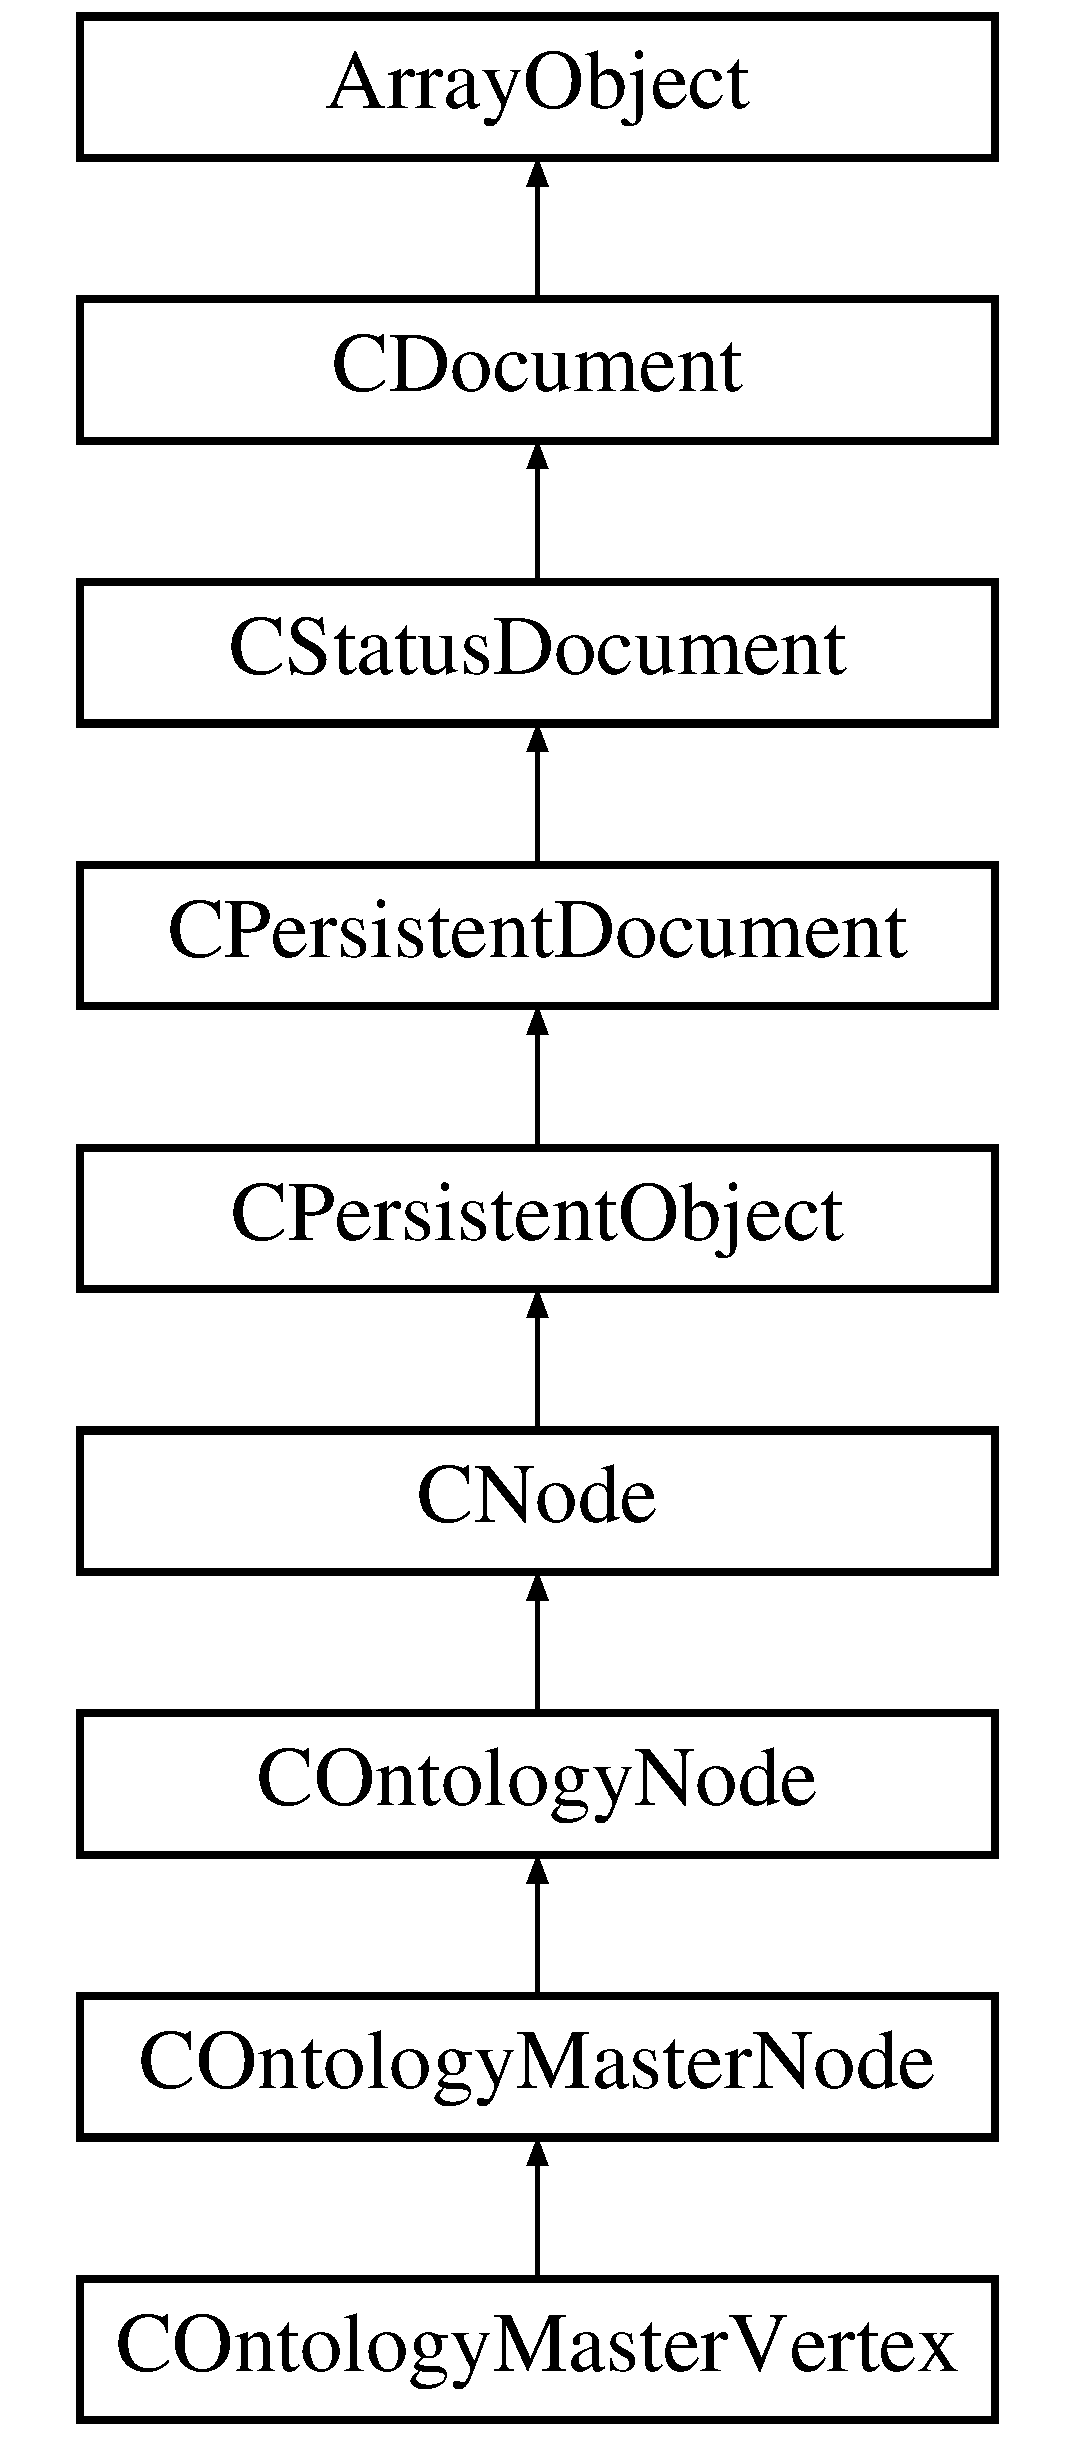
\includegraphics[height=9.000000cm]{class_c_ontology_master_node}
\end{center}
\end{figure}
\subsection*{Public Member Functions}
\begin{DoxyCompactItemize}
\item 
\hyperlink{class_c_ontology_master_node_a1dbcd0aa39c97027ebf020eda30c9c85}{Node\-Refs} ()
\item 
\hyperlink{class_c_ontology_master_node_a3b17a7706f8297c2735bd8035995762a}{Relate\-To} (\$the\-Predicate, \$the\-Object, \$the\-Connection=N\-U\-L\-L, \$do\-Propagate=T\-R\-U\-E)
\end{DoxyCompactItemize}
\subsection*{Static Public Member Functions}
\begin{DoxyCompactItemize}
\item 
static \hyperlink{class_c_ontology_master_node_a29aadfcab71c78e4f4a107aad67a8ebe}{Resolve} (\hyperlink{class_c_connection}{C\-Connection} \$the\-Connection, \$the\-Identifier, \$do\-Throw=F\-A\-L\-S\-E)
\end{DoxyCompactItemize}
\subsection*{Protected Member Functions}
\begin{DoxyCompactItemize}
\item 
\hyperlink{class_c_ontology_master_node_a6bff75981a894a0b25a3ed64a8966478}{\-\_\-\-Precommit\-Identify} (\&\$the\-Connection, \&\$the\-Modifiers)
\end{DoxyCompactItemize}
\subsection*{Additional Inherited Members}


\subsection{Member Function Documentation}
\hypertarget{class_c_ontology_master_node_a6bff75981a894a0b25a3ed64a8966478}{\index{C\-Ontology\-Master\-Node@{C\-Ontology\-Master\-Node}!\-\_\-\-Precommit\-Identify@{\-\_\-\-Precommit\-Identify}}
\index{\-\_\-\-Precommit\-Identify@{\-\_\-\-Precommit\-Identify}!COntologyMasterNode@{C\-Ontology\-Master\-Node}}
\subsubsection[{\-\_\-\-Precommit\-Identify}]{\setlength{\rightskip}{0pt plus 5cm}C\-Ontology\-Master\-Node\-::\-\_\-\-Precommit\-Identify (
\begin{DoxyParamCaption}
\item[{\&}]{\$the\-Connection, }
\item[{\&}]{\$the\-Modifiers}
\end{DoxyParamCaption}
)\hspace{0.3cm}{\ttfamily [protected]}}}\label{class_c_ontology_master_node_a6bff75981a894a0b25a3ed64a8966478}
\subparagraph*{Determine the identifiers before committing}

We overload this method to prevent creating two nodes that refer to the same term. We first check if there is another node that refers to the same term and that does point to another node\-: if we find one we add the \hyperlink{}{k\-T\-A\-G\-\_\-\-C\-A\-T\-E\-G\-O\-R\-Y}, \hyperlink{}{k\-T\-A\-G\-\_\-\-K\-I\-N\-D}, \hyperlink{}{k\-T\-A\-G\-\_\-\-T\-Y\-P\-E}, \hyperlink{}{k\-T\-A\-G\-\_\-\-I\-N\-P\-U\-T} and \hyperlink{}{k\-T\-A\-G\-\_\-\-E\-X\-A\-M\-P\-L\-E\-S} attributes to the found node and make it the current node; if no such node is found, we call the parent method.

In the first case we return the found node identifier, this will stop the commit workflow.


\begin{DoxyParams}[1]{Parameters}
reference & {\em \&\$the\-Connection} & Server, database or container. \\
\hline
reference & {\em \&\$the\-Modifiers} & Commit options.\\
\hline
\end{DoxyParams}
protected \begin{DoxyReturn}{Returns}
mixed
\end{DoxyReturn}
\begin{DoxySeeAlso}{See Also}
k\-T\-A\-G\-\_\-\-N\-I\-D k\-S\-E\-Q\-U\-E\-N\-C\-E\-\_\-\-K\-E\-Y\-\_\-\-N\-O\-D\-E 

k\-F\-L\-A\-G\-\_\-\-P\-E\-R\-S\-I\-S\-T\-\_\-\-I\-N\-S\-E\-R\-T k\-F\-L\-A\-G\-\_\-\-P\-E\-R\-S\-I\-S\-T\-\_\-\-R\-E\-P\-L\-A\-C\-E 
\end{DoxySeeAlso}
\hypertarget{class_c_ontology_master_node_a1dbcd0aa39c97027ebf020eda30c9c85}{\index{C\-Ontology\-Master\-Node@{C\-Ontology\-Master\-Node}!Node\-Refs@{Node\-Refs}}
\index{Node\-Refs@{Node\-Refs}!COntologyMasterNode@{C\-Ontology\-Master\-Node}}
\subsubsection[{Node\-Refs}]{\setlength{\rightskip}{0pt plus 5cm}C\-Ontology\-Master\-Node\-::\-Node\-Refs (
\begin{DoxyParamCaption}
{}
\end{DoxyParamCaption}
)}}\label{class_c_ontology_master_node_a1dbcd0aa39c97027ebf020eda30c9c85}
\subparagraph*{Manage node references}

The {\itshape node references}, \hyperlink{}{k\-T\-A\-G\-\_\-\-N\-O\-D\-E\-S}, holds a list of identifiers of alias nodes that reference the current node.

The method is read-\/only, because this value must be managed externally.

public \begin{DoxyReturn}{Returns}
array Nodes reference list.
\end{DoxyReturn}
\begin{DoxySeeAlso}{See Also}
k\-T\-A\-G\-\_\-\-N\-O\-D\-E\-S 
\end{DoxySeeAlso}
\hypertarget{class_c_ontology_master_node_a3b17a7706f8297c2735bd8035995762a}{\index{C\-Ontology\-Master\-Node@{C\-Ontology\-Master\-Node}!Relate\-To@{Relate\-To}}
\index{Relate\-To@{Relate\-To}!COntologyMasterNode@{C\-Ontology\-Master\-Node}}
\subsubsection[{Relate\-To}]{\setlength{\rightskip}{0pt plus 5cm}C\-Ontology\-Master\-Node\-::\-Relate\-To (
\begin{DoxyParamCaption}
\item[{}]{\$the\-Predicate, }
\item[{}]{\$the\-Object, }
\item[{}]{\$the\-Connection = {\ttfamily NULL}, }
\item[{}]{\$do\-Propagate = {\ttfamily TRUE}}
\end{DoxyParamCaption}
)}}\label{class_c_ontology_master_node_a3b17a7706f8297c2735bd8035995762a}
\subparagraph*{Relate to node}

We overload this method to mirror relationships between alias nodes to their counterpart master nodes, this is governed by the {\ttfamily \$do\-Propagate} switch.

We first create the requested relationship, then, if the object is an alias, we relate the current object with the object's master.

This means that\-:


\begin{DoxyItemize}
\item {\itshape M\-A\-S\-T\-E\-R =$>$ M\-A\-S\-T\-E\-R}\-: 
\begin{DoxyItemize}
\item M\-A\-S\-T\-E\-R =$>$ M\-A\-S\-T\-E\-R 
\end{DoxyItemize}
\item {\itshape M\-A\-S\-T\-E\-R =$>$ A\-L\-I\-A\-S}\-: 
\begin{DoxyItemize}
\item M\-A\-S\-T\-E\-R =$>$ A\-L\-I\-A\-S 
\item M\-A\-S\-T\-E\-R =$>$ A\-L\-I\-A\-S.\-M\-A\-S\-T\-E\-R 
\end{DoxyItemize}
\end{DoxyItemize}

Note that this method is called by its counterpart in \hyperlink{class_c_ontology_alias_node}{C\-Ontology\-Alias\-Node}, this means

We require the connection parameter here since both subject and object vertices must be committed by this method, this implies that the edge will also be committed.


\begin{DoxyParams}[1]{Parameters}
mixed & {\em \$the\-Predicate} & Predicate term object or reference. \\
\hline
mixed & {\em \$the\-Object} & Object node object or reference. \\
\hline
\hyperlink{class_c_connection}{C\-Connection} & {\em \$the\-Connection} & Server, database or container. \\
\hline
boolean & {\em \$do\-Propagate} & T\-R\-U\-E means relate masters.\\
\hline
\end{DoxyParams}
public \begin{DoxyReturn}{Returns}
\hyperlink{class_c_ontology_edge}{C\-Ontology\-Edge} Edge object. 
\end{DoxyReturn}
\hypertarget{class_c_ontology_master_node_a29aadfcab71c78e4f4a107aad67a8ebe}{\index{C\-Ontology\-Master\-Node@{C\-Ontology\-Master\-Node}!Resolve@{Resolve}}
\index{Resolve@{Resolve}!COntologyMasterNode@{C\-Ontology\-Master\-Node}}
\subsubsection[{Resolve}]{\setlength{\rightskip}{0pt plus 5cm}static C\-Ontology\-Master\-Node\-::\-Resolve (
\begin{DoxyParamCaption}
\item[{{\bf C\-Connection}}]{\$the\-Connection, }
\item[{}]{\$the\-Identifier, }
\item[{}]{\$do\-Throw = {\ttfamily FALSE}}
\end{DoxyParamCaption}
)\hspace{0.3cm}{\ttfamily [static]}}}\label{class_c_ontology_master_node_a29aadfcab71c78e4f4a107aad67a8ebe}
\subparagraph*{Resolve a node}

We overload this method in this class by intercepting all cases in which the {\ttfamily \$the\-Identifier} is not an integer, or node reference\-: since no two nodes of this class can share the same term reference, we add a clause to the search query to exclude all node that have a \hyperlink{}{k\-T\-A\-G\-\_\-\-N\-O\-D\-E} attribute. We do this rather than use the object class, because we assume all nodes that have the \hyperlink{}{k\-T\-A\-G\-\_\-\-N\-O\-D\-E} attribute to be aliases.

Since terms become also a unique identifier, this method will return either an object or {\ttfamily N\-U\-L\-L}.


\begin{DoxyParams}[1]{Parameters}
\hyperlink{class_c_connection}{C\-Connection} & {\em \$the\-Connection} & Server, database or container. \\
\hline
mixed & {\em \$the\-Identifier} & Node identifier or term reference. \\
\hline
boolean & {\em \$do\-Throw} & If {\ttfamily T\-R\-U\-E} raise an exception.\\
\hline
\end{DoxyParams}
\begin{DoxyReturn}{Returns}
\hyperlink{class_c_ontology_master_node}{C\-Ontology\-Master\-Node} Matched node, found nodes or {\ttfamily N\-U\-L\-L}.
\end{DoxyReturn}

\begin{DoxyExceptions}{Exceptions}
{\em Exception} & \\
\hline
\end{DoxyExceptions}


The documentation for this class was generated from the following file\-:\begin{DoxyCompactItemize}
\item 
/\-Library/\-Web\-Server/\-Library/\-P\-H\-P\-Wrapper/classes/C\-Ontology\-Master\-Node.\-php\end{DoxyCompactItemize}

\hypertarget{class_c_ontology_master_vertex}{\section{C\-Ontology\-Master\-Vertex Class Reference}
\label{class_c_ontology_master_vertex}\index{C\-Ontology\-Master\-Vertex@{C\-Ontology\-Master\-Vertex}}
}
Inheritance diagram for C\-Ontology\-Master\-Vertex\-:\begin{figure}[H]
\begin{center}
\leavevmode
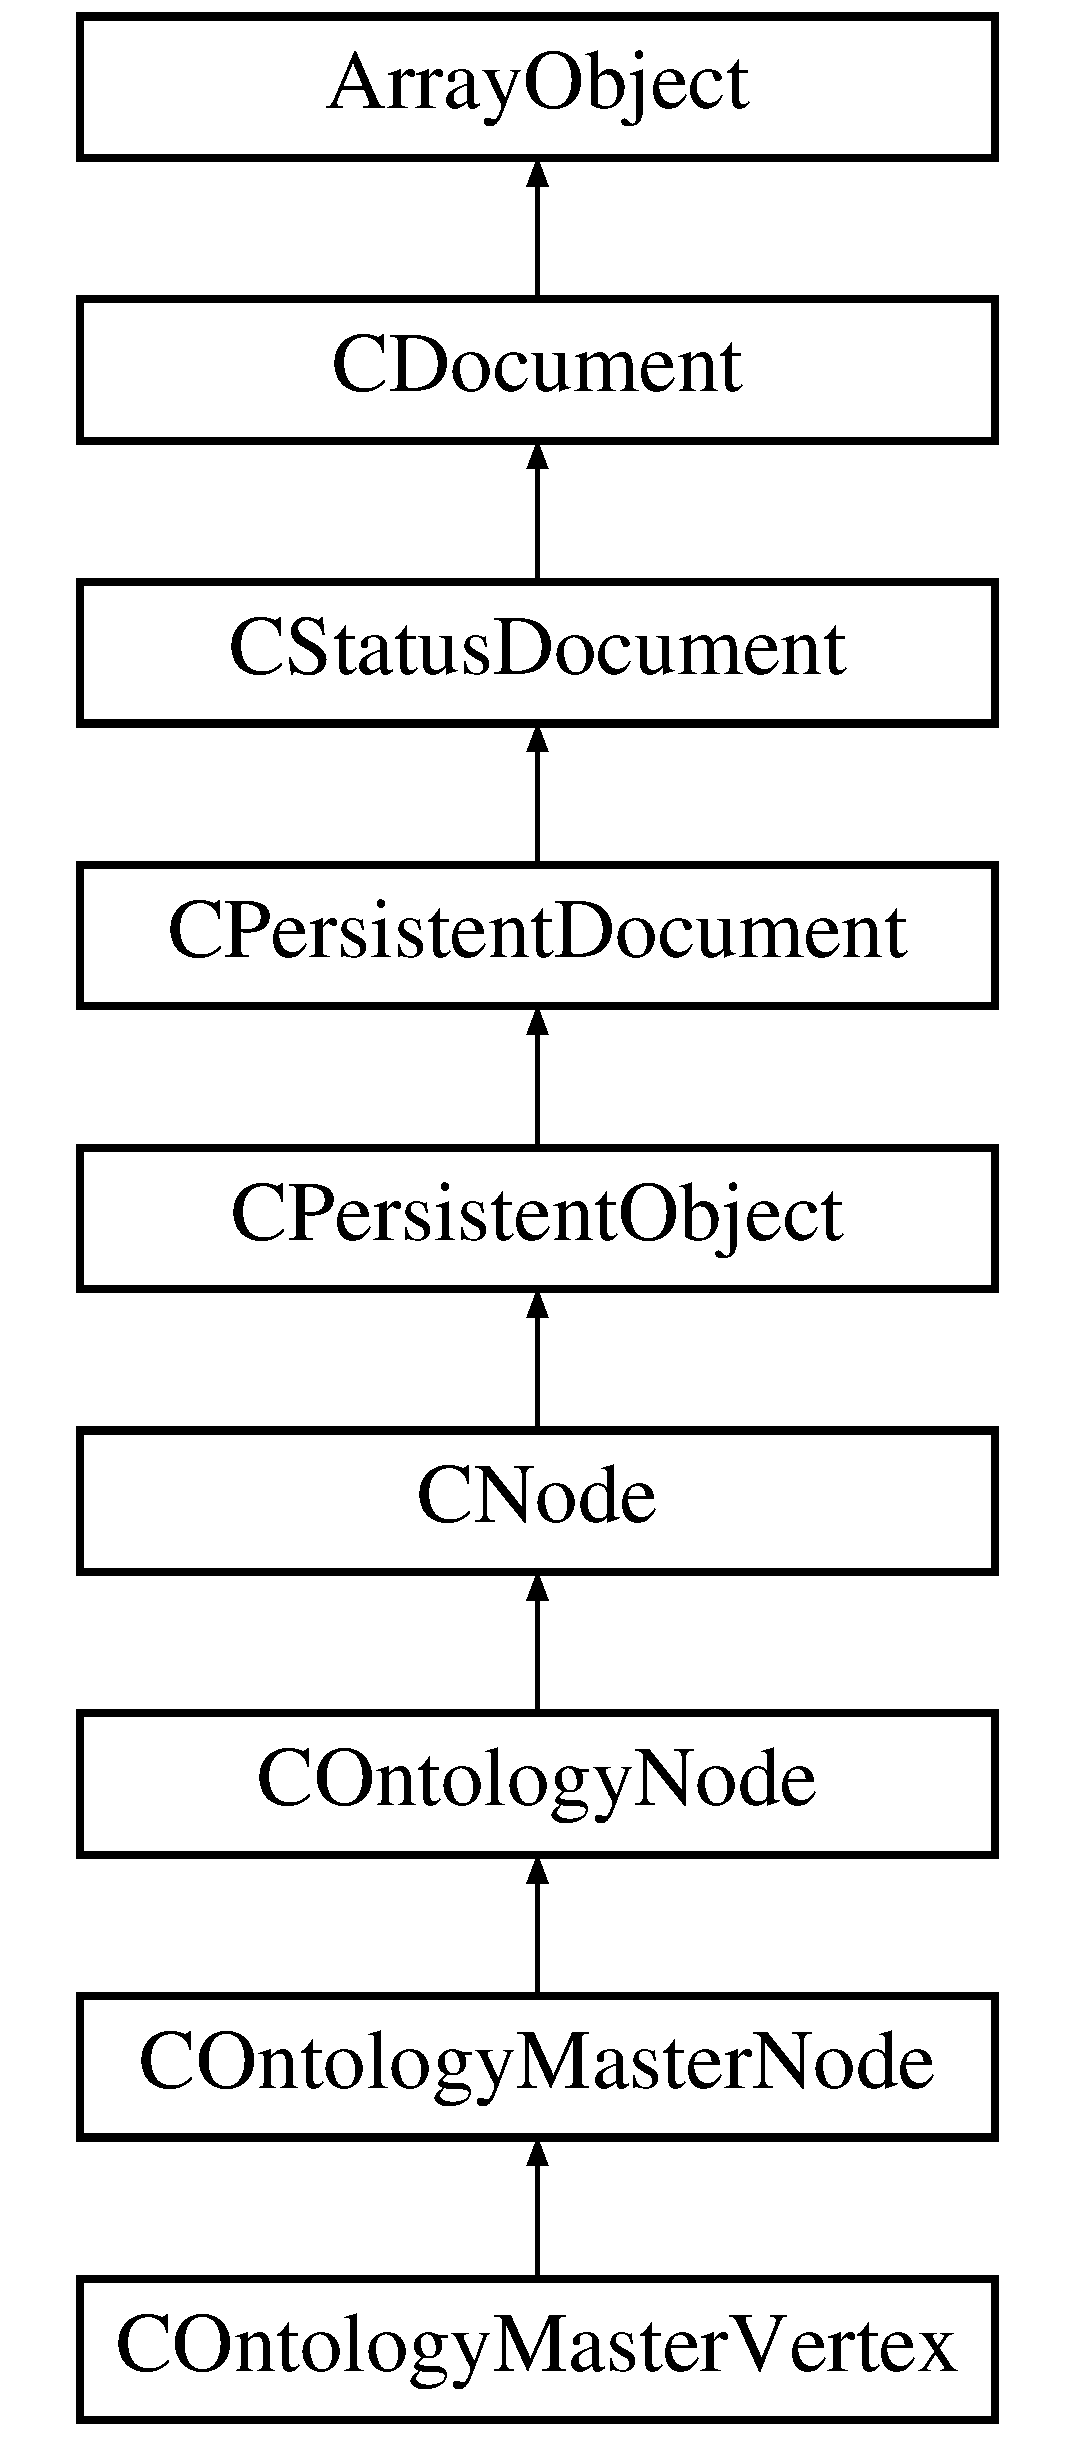
\includegraphics[height=9.000000cm]{class_c_ontology_master_vertex}
\end{center}
\end{figure}
\subsection*{Protected Member Functions}
\begin{DoxyCompactItemize}
\item 
\hyperlink{class_c_ontology_master_vertex_a054fdaa67952efb59dc30b47ceed8781}{\-\_\-\-Term\-Attributes} ()
\end{DoxyCompactItemize}
\subsection*{Additional Inherited Members}


\subsection{Member Function Documentation}
\hypertarget{class_c_ontology_master_vertex_a054fdaa67952efb59dc30b47ceed8781}{\index{C\-Ontology\-Master\-Vertex@{C\-Ontology\-Master\-Vertex}!\-\_\-\-Term\-Attributes@{\-\_\-\-Term\-Attributes}}
\index{\-\_\-\-Term\-Attributes@{\-\_\-\-Term\-Attributes}!COntologyMasterVertex@{C\-Ontology\-Master\-Vertex}}
\subsubsection[{\-\_\-\-Term\-Attributes}]{\setlength{\rightskip}{0pt plus 5cm}C\-Ontology\-Master\-Vertex\-::\-\_\-\-Term\-Attributes (
\begin{DoxyParamCaption}
{}
\end{DoxyParamCaption}
)\hspace{0.3cm}{\ttfamily [protected]}}}\label{class_c_ontology_master_vertex_a054fdaa67952efb59dc30b47ceed8781}
\subparagraph*{List term attributes}

In this class we return\-:


\begin{DoxyItemize}
\item {\ttfamily \hyperlink{}{k\-T\-A\-G\-\_\-\-L\-I\-D}}\-: The local identifier. 
\item {\ttfamily \hyperlink{}{k\-T\-A\-G\-\_\-\-G\-I\-D}}\-: The global identifier. 
\item {\ttfamily \hyperlink{}{k\-T\-A\-G\-\_\-\-L\-A\-B\-E\-L}}\-: The label. 
\item {\ttfamily \hyperlink{}{k\-T\-A\-G\-\_\-\-D\-E\-F\-I\-N\-I\-T\-I\-O\-N}}\-: The definition. 
\item {\ttfamily \hyperlink{}{k\-T\-A\-G\-\_\-\-F\-E\-A\-T\-U\-R\-E\-S}}\-: The feature tag references. 
\item {\ttfamily \hyperlink{}{k\-T\-A\-G\-\_\-\-S\-C\-A\-L\-E\-S}}\-: The scale tag references. 
\end{DoxyItemize}

protected \begin{DoxyReturn}{Returns}
array 
\end{DoxyReturn}


The documentation for this class was generated from the following file\-:\begin{DoxyCompactItemize}
\item 
/\-Library/\-Web\-Server/\-Library/\-P\-H\-P\-Wrapper/classes/C\-Ontology\-Master\-Vertex.\-php\end{DoxyCompactItemize}

\hypertarget{class_c_ontology_node}{\section{C\-Ontology\-Node Class Reference}
\label{class_c_ontology_node}\index{C\-Ontology\-Node@{C\-Ontology\-Node}}
}
Inheritance diagram for C\-Ontology\-Node\-:\begin{figure}[H]
\begin{center}
\leavevmode
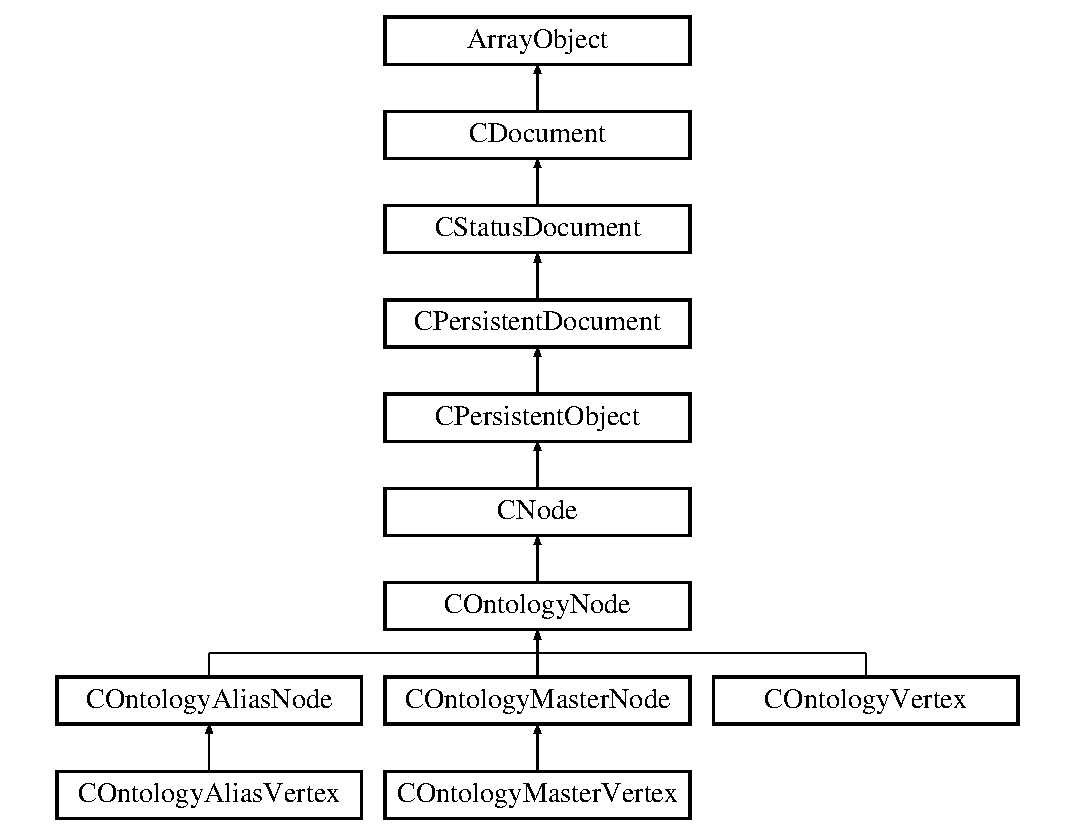
\includegraphics[height=9.000000cm]{class_c_ontology_node}
\end{center}
\end{figure}
\subsection*{Public Member Functions}
\begin{DoxyCompactItemize}
\item 
\hyperlink{class_c_ontology_node_ae074c6f51676b4ef5fc3d7fd1c3149af}{\-\_\-\-\_\-to\-String} ()
\item 
\hyperlink{class_c_ontology_node_afc2d00b2e6dd8ecc37d87a593581bc3a}{Type} (\$the\-Value=N\-U\-L\-L, \$the\-Operation=N\-U\-L\-L, \$get\-Old=F\-A\-L\-S\-E)
\item 
\hyperlink{class_c_ontology_node_a09eb3d9d16775d7752fd7bf62dd93d74}{Load\-Term} (\hyperlink{class_c_connection}{C\-Connection} \$the\-Connection, \$do\-Reload=F\-A\-L\-S\-E)
\item 
\hyperlink{class_c_ontology_node_a0dc5644213c5599332a024af2160c9f1}{Get\-Graph\-Node} (\hyperlink{class_c_connection}{C\-Connection} \$the\-Connection, \$the\-Identifier=N\-U\-L\-L)
\item 
\hyperlink{class_c_ontology_node_a8da921e4518e6c9bfc0f2ce6eefe7697}{Get\-Graph\-Node\-Properties} (\hyperlink{class_c_connection}{C\-Connection} \$the\-Connection, \$the\-Identifier=N\-U\-L\-L)
\item 
\hyperlink{class_c_ontology_node_a249a067e22e3d721958903e5b6c36b84}{Update} (\hyperlink{class_c_connection}{C\-Connection} \$the\-Connection)
\item 
\hyperlink{class_c_ontology_node_afc20c775f2ae9e01a2d8e50c95b00baf}{Replace} (\hyperlink{class_c_connection}{C\-Connection} \$the\-Connection)
\end{DoxyCompactItemize}
\subsection*{Static Public Member Functions}
\begin{DoxyCompactItemize}
\item 
static \hyperlink{class_c_ontology_node_a66c5bc42f0cbb921105795127fa816cf}{Default\-Container\-Name} ()
\item 
static \hyperlink{class_c_ontology_node_af249fcb695d7d3ceeed5a74446df0822}{Resolve} (\hyperlink{class_c_connection}{C\-Connection} \$the\-Connection, \$the\-Identifier, \$do\-Throw=F\-A\-L\-S\-E)
\item 
static \hyperlink{class_c_ontology_node_aa29329d76906e4d2a5f5589a909074a1}{Resolve\-P\-I\-D} (\hyperlink{class_c_connection}{C\-Connection} \$the\-Connection, \$the\-Identifier, \$do\-Throw=F\-A\-L\-S\-E, \$do\-Object=F\-A\-L\-S\-E)
\end{DoxyCompactItemize}
\subsection*{Protected Member Functions}
\begin{DoxyCompactItemize}
\item 
\hyperlink{class_c_ontology_node_a75c282c323e10fed112e14488d5962c5}{\-\_\-\-Preset} (\&\$the\-Offset, \&\$the\-Value)
\item 
\hyperlink{class_c_ontology_node_a93662baceebafc3d02904083aaab7c29}{\-\_\-\-Preunset} (\&\$the\-Offset)
\item 
\hyperlink{class_c_ontology_node_acc47d27e9a861190b00a6efb39f7c825}{\-\_\-\-Precommit\-Related} (\&\$the\-Connection, \&\$the\-Modifiers)
\item 
\hyperlink{class_c_ontology_node_aca703ceb64a2175b2b432bf50874015a}{\-\_\-\-Precommit\-Identify} (\&\$the\-Connection, \&\$the\-Modifiers)
\item 
\hyperlink{class_c_ontology_node_a2a86e54a0b6336b3014eb3dc0f41a103}{\-\_\-\-Postcommit\-Related} (\&\$the\-Connection, \&\$the\-Modifiers)
\item 
\hyperlink{class_c_ontology_node_afee8b58f970fe3ff8bc07ef80c771558}{\-\_\-\-Postcommit\-Cleanup} (\&\$the\-Connection, \&\$the\-Modifiers)
\item 
\hyperlink{class_c_ontology_node_a140f5db26f804f0347f09b3959ed75da}{\-\_\-\-Load\-Term\-Attributes} (\$the\-Attributes=N\-U\-L\-L)
\item 
\hyperlink{class_c_ontology_node_a0dd83a16ead60eba2e6782f1dfab2f72}{\-\_\-\-Term\-Attributes} ()
\item 
\hyperlink{class_c_ontology_node_aa91367053433a0bdd052650f9eb54a7c}{\-\_\-\-Add\-Graph\-Node} (\hyperlink{class_c_graph_container}{C\-Graph\-Container} \$the\-Graph, \$the\-Identifier=N\-U\-L\-L, \$the\-Properties=N\-U\-L\-L)
\item 
\hyperlink{class_c_ontology_node_a1b13e21b3b634b6fd66d5dce38a79b9a}{\-\_\-\-Graph\-Node\-Properties} (\$the\-Properties=N\-U\-L\-L)
\item 
\hyperlink{class_c_ontology_node_a1b559f9ace69d7768a7acb8a7364d493}{\-\_\-\-New\-Edge} ()
\end{DoxyCompactItemize}
\subsection*{Protected Attributes}
\begin{DoxyCompactItemize}
\item 
\hypertarget{class_c_ontology_node_a23aa9d9d9cde004bc251dc98c192652d}{{\bfseries \$m\-Term} = N\-U\-L\-L}\label{class_c_ontology_node_a23aa9d9d9cde004bc251dc98c192652d}

\end{DoxyCompactItemize}


\subsection{Member Function Documentation}
\hypertarget{class_c_ontology_node_ae074c6f51676b4ef5fc3d7fd1c3149af}{\index{C\-Ontology\-Node@{C\-Ontology\-Node}!\-\_\-\-\_\-to\-String@{\-\_\-\-\_\-to\-String}}
\index{\-\_\-\-\_\-to\-String@{\-\_\-\-\_\-to\-String}!COntologyNode@{C\-Ontology\-Node}}
\subsubsection[{\-\_\-\-\_\-to\-String}]{\setlength{\rightskip}{0pt plus 5cm}C\-Ontology\-Node\-::\-\_\-\-\_\-to\-String (
\begin{DoxyParamCaption}
{}
\end{DoxyParamCaption}
)}}\label{class_c_ontology_node_ae074c6f51676b4ef5fc3d7fd1c3149af}
\subparagraph*{Return object name}

This method should return the current object's name which should represent the unique identifier of the object.

By default we return the string representation of the term, \hyperlink{}{k\-T\-A\-G\-\_\-\-T\-E\-R\-M}.

public \begin{DoxyReturn}{Returns}
string The connection name. 
\end{DoxyReturn}
\hypertarget{class_c_ontology_node_aa91367053433a0bdd052650f9eb54a7c}{\index{C\-Ontology\-Node@{C\-Ontology\-Node}!\-\_\-\-Add\-Graph\-Node@{\-\_\-\-Add\-Graph\-Node}}
\index{\-\_\-\-Add\-Graph\-Node@{\-\_\-\-Add\-Graph\-Node}!COntologyNode@{C\-Ontology\-Node}}
\subsubsection[{\-\_\-\-Add\-Graph\-Node}]{\setlength{\rightskip}{0pt plus 5cm}C\-Ontology\-Node\-::\-\_\-\-Add\-Graph\-Node (
\begin{DoxyParamCaption}
\item[{{\bf C\-Graph\-Container}}]{\$the\-Graph, }
\item[{}]{\$the\-Identifier = {\ttfamily NULL}, }
\item[{}]{\$the\-Properties = {\ttfamily NULL}}
\end{DoxyParamCaption}
)\hspace{0.3cm}{\ttfamily [protected]}}}\label{class_c_ontology_node_aa91367053433a0bdd052650f9eb54a7c}
\subparagraph*{Create or update a graph node}

This method will create and save a new graph node in the provided graph container and return its newly created identifier, or retrieve a graph node and update its properties.

This method is called by \hyperlink{class_c_ontology_node_aca703ceb64a2175b2b432bf50874015a}{\-\_\-\-Precommit\-Identify()} to set the new node \hyperlink{}{k\-T\-A\-G\-\_\-\-N\-I\-D} and from other methods to update the node properties.

This method will use the \hyperlink{class_c_ontology_node_a1b13e21b3b634b6fd66d5dce38a79b9a}{\-\_\-\-Graph\-Node\-Properties()} method to determine which attributes will be set in the graph node.

The method expects the following parameters\-:


\begin{DoxyItemize}
\item {\ttfamily \$the\-Graph}\-: The graph container or client. 
\item {\ttfamily \$the\-Identifier}\-: The graph node identifier, if provided, it means that we want to update an existing graph node and the parameter is its identifier. If the node cannot be located in the graph, the method should raise an exception. If the parameter is not provided, it means that we want to create a new graph node. 
\item {\ttfamily \$the\-Properties}\-: The graph node properties, if provided, the new or existing node will have its properties replaced with the ones in this parameter; if not provided, the \hyperlink{class_c_ontology_node_a1b13e21b3b634b6fd66d5dce38a79b9a}{\-\_\-\-Graph\-Node\-Properties()} method will be used to extract the required properties from the current node and update or set the graph node's. 
\end{DoxyItemize}

The method should raise an exception if the operation fails.


\begin{DoxyParams}[1]{Parameters}
\hyperlink{class_c_graph_container}{C\-Graph\-Container} & {\em \$the\-Graph} & Graph container. \\
\hline
integer & {\em \$the\-Identifier} & Graph node identifier. \\
\hline
array & {\em \$the\-Properties} & Graph node properties.\\
\hline
\end{DoxyParams}
protected \begin{DoxyReturn}{Returns}
integer Newly created or existing node I\-D. 
\end{DoxyReturn}
\hypertarget{class_c_ontology_node_a1b13e21b3b634b6fd66d5dce38a79b9a}{\index{C\-Ontology\-Node@{C\-Ontology\-Node}!\-\_\-\-Graph\-Node\-Properties@{\-\_\-\-Graph\-Node\-Properties}}
\index{\-\_\-\-Graph\-Node\-Properties@{\-\_\-\-Graph\-Node\-Properties}!COntologyNode@{C\-Ontology\-Node}}
\subsubsection[{\-\_\-\-Graph\-Node\-Properties}]{\setlength{\rightskip}{0pt plus 5cm}C\-Ontology\-Node\-::\-\_\-\-Graph\-Node\-Properties (
\begin{DoxyParamCaption}
\item[{}]{\$the\-Properties = {\ttfamily NULL}}
\end{DoxyParamCaption}
)\hspace{0.3cm}{\ttfamily [protected]}}}\label{class_c_ontology_node_a1b13e21b3b634b6fd66d5dce38a79b9a}
\subparagraph*{Return the list of graph node tags}

This method should return an array of attributes which represents the list of properties which should be transferred to the graph node.

This method can be overloaded as more specialised node classes are developed, the main reason for this method is to control which properties should be copied to the graph and which properties are supported by the graph nodes.

The method accepts an optional parameter, {\ttfamily \$the\-Properties}, which represents an array of attributes that can be filtered by this method\-: only those elements which match the tags supported by this method will be selected. This parameter can be an array or Array\-Object, any other type will trigger an exception.

In this class we copy the \hyperlink{}{k\-T\-A\-G\-\_\-\-G\-I\-D}, \hyperlink{}{k\-T\-A\-G\-\_\-\-C\-A\-T\-E\-G\-O\-R\-Y}, \hyperlink{}{k\-T\-A\-G\-\_\-\-K\-I\-N\-D} and \hyperlink{}{k\-T\-A\-G\-\_\-\-T\-Y\-P\-E} attributes. Note that the \hyperlink{}{k\-T\-A\-G\-\_\-\-G\-I\-D} attribute will only be copied in derived classes that add that term's attribute to the current node.


\begin{DoxyParams}[1]{Parameters}
array & {\em \$the\-Properties} & Base properties.\\
\hline
\end{DoxyParams}
protected \begin{DoxyReturn}{Returns}
array List of properties. 
\end{DoxyReturn}
\hypertarget{class_c_ontology_node_a140f5db26f804f0347f09b3959ed75da}{\index{C\-Ontology\-Node@{C\-Ontology\-Node}!\-\_\-\-Load\-Term\-Attributes@{\-\_\-\-Load\-Term\-Attributes}}
\index{\-\_\-\-Load\-Term\-Attributes@{\-\_\-\-Load\-Term\-Attributes}!COntologyNode@{C\-Ontology\-Node}}
\subsubsection[{\-\_\-\-Load\-Term\-Attributes}]{\setlength{\rightskip}{0pt plus 5cm}C\-Ontology\-Node\-::\-\_\-\-Load\-Term\-Attributes (
\begin{DoxyParamCaption}
\item[{}]{\$the\-Attributes = {\ttfamily NULL}}
\end{DoxyParamCaption}
)\hspace{0.3cm}{\ttfamily [protected]}}}\label{class_c_ontology_node_a140f5db26f804f0347f09b3959ed75da}
\subparagraph*{Load term attributes}

This method can be used to copy selected term attributes to the current object, this is used to cache searchable term attributes directly in the node, to prevent having to search both terms and nodes.

The method accepts a single parameter, {\ttfamily \$the\-Attributes}, which is the list of term attribute tags which should be copied to this object. If the parameter is omitted, the method will copy all attributes.

This method will first load the term attributes, then overwrite them with the node attributes, this effectively makes matching node attributes overwrite term attributes.

The method is called by \hyperlink{class_c_persistent_document_a23cfbb5ebf75e008622ab9e723472c70}{\-\_\-\-Precommit()}, in derived classes you can call the parent method and add custom attributes in the derived method.

In this class this method is not called, in derived classes you should explicitly invoke it.


\begin{DoxyParams}[1]{Parameters}
array & {\em \$the\-Attributes} & Term attribute tags list.\\
\hline
\end{DoxyParams}
protected

\begin{DoxySeeAlso}{See Also}
k\-T\-A\-G\-\_\-\-T\-E\-R\-M k\-T\-A\-G\-\_\-\-N\-O\-D\-E\-S 

k\-F\-L\-A\-G\-\_\-\-P\-E\-R\-S\-I\-S\-T\-\_\-\-M\-O\-D\-I\-F\-Y k\-F\-L\-A\-G\-\_\-\-M\-O\-D\-I\-F\-Y\-\_\-\-A\-D\-D\-S\-E\-T k\-F\-L\-A\-G\-\_\-\-M\-O\-D\-I\-F\-Y\-\_\-\-P\-U\-L\-L 
\end{DoxySeeAlso}
\hypertarget{class_c_ontology_node_a1b559f9ace69d7768a7acb8a7364d493}{\index{C\-Ontology\-Node@{C\-Ontology\-Node}!\-\_\-\-New\-Edge@{\-\_\-\-New\-Edge}}
\index{\-\_\-\-New\-Edge@{\-\_\-\-New\-Edge}!COntologyNode@{C\-Ontology\-Node}}
\subsubsection[{\-\_\-\-New\-Edge}]{\setlength{\rightskip}{0pt plus 5cm}C\-Ontology\-Node\-::\-\_\-\-New\-Edge (
\begin{DoxyParamCaption}
{}
\end{DoxyParamCaption}
)\hspace{0.3cm}{\ttfamily [protected]}}}\label{class_c_ontology_node_a1b559f9ace69d7768a7acb8a7364d493}
\subparagraph*{Return a new edge instance}

In this class we return a \hyperlink{class_c_ontology_edge}{C\-Ontology\-Edge} instance.

protected \begin{DoxyReturn}{Returns}
\hyperlink{class_c_edge}{C\-Edge} 
\end{DoxyReturn}
\hypertarget{class_c_ontology_node_afee8b58f970fe3ff8bc07ef80c771558}{\index{C\-Ontology\-Node@{C\-Ontology\-Node}!\-\_\-\-Postcommit\-Cleanup@{\-\_\-\-Postcommit\-Cleanup}}
\index{\-\_\-\-Postcommit\-Cleanup@{\-\_\-\-Postcommit\-Cleanup}!COntologyNode@{C\-Ontology\-Node}}
\subsubsection[{\-\_\-\-Postcommit\-Cleanup}]{\setlength{\rightskip}{0pt plus 5cm}C\-Ontology\-Node\-::\-\_\-\-Postcommit\-Cleanup (
\begin{DoxyParamCaption}
\item[{\&}]{\$the\-Connection, }
\item[{\&}]{\$the\-Modifiers}
\end{DoxyParamCaption}
)\hspace{0.3cm}{\ttfamily [protected]}}}\label{class_c_ontology_node_afee8b58f970fe3ff8bc07ef80c771558}
\subparagraph*{Cleanup the object after committing}

In this class we reset the term object cache, we set the data member to {\ttfamily N\-U\-L\-L} so that next time one wants to retrieve the term object, it will have to be refreshed and its references actualised.


\begin{DoxyParams}[1]{Parameters}
reference & {\em \&\$the\-Connection} & Server, database or container. \\
\hline
reference & {\em \&\$the\-Modifiers} & Commit options.\\
\hline
\end{DoxyParams}
protected \hypertarget{class_c_ontology_node_a2a86e54a0b6336b3014eb3dc0f41a103}{\index{C\-Ontology\-Node@{C\-Ontology\-Node}!\-\_\-\-Postcommit\-Related@{\-\_\-\-Postcommit\-Related}}
\index{\-\_\-\-Postcommit\-Related@{\-\_\-\-Postcommit\-Related}!COntologyNode@{C\-Ontology\-Node}}
\subsubsection[{\-\_\-\-Postcommit\-Related}]{\setlength{\rightskip}{0pt plus 5cm}C\-Ontology\-Node\-::\-\_\-\-Postcommit\-Related (
\begin{DoxyParamCaption}
\item[{\&}]{\$the\-Connection, }
\item[{\&}]{\$the\-Modifiers}
\end{DoxyParamCaption}
)\hspace{0.3cm}{\ttfamily [protected]}}}\label{class_c_ontology_node_a2a86e54a0b6336b3014eb3dc0f41a103}
\subparagraph*{Update related objects after committing}

In this class we handle referenced terms, \hyperlink{}{k\-T\-A\-G\-\_\-\-T\-E\-R\-M}\-: depending on the value of the \hyperlink{}{k\-S\-W\-I\-T\-C\-H\-\_\-k\-T\-A\-G\-\_\-\-N\-O\-D\-E\-S} flag we do the following\-:


\begin{DoxyItemize}
\item {\ttfamily 0x2}\-: {\itshape Keep count of references}. This means that the \hyperlink{}{k\-T\-A\-G\-\_\-\-N\-O\-D\-E\-S} attribute of the term referenced by the \hyperlink{}{k\-T\-A\-G\-\_\-\-T\-E\-R\-M} attribute will be incremented when the object is inserted, or decremented when deleted. 
\item {\ttfamily 0x3}\-: {\itshape Keep list of references}. This means that a reference to the current object will be added to the \hyperlink{}{k\-T\-A\-G\-\_\-\-N\-O\-D\-E\-S} attribute of the term referenced by \hyperlink{}{k\-T\-A\-G\-\_\-\-T\-E\-R\-M} attribute of the current object when the latter is inserted, and removed when the object is deleted. 
\item {\ttfamily 0x0} {\itshape or other}\-: {\itshape Don't handle this information}. This means that the \hyperlink{}{k\-T\-A\-G\-\_\-\-N\-O\-D\-E\-S} attribute will not be handled. 
\end{DoxyItemize}

Note that you should provide either a database connection or the {\itshape term} container to this method in order to make it work!


\begin{DoxyParams}[1]{Parameters}
reference & {\em \&\$the\-Connection} & Server, database or container. \\
\hline
reference & {\em \&\$the\-Modifiers} & Commit options.\\
\hline
\end{DoxyParams}
protected

\hyperlink{class_c_status_document_ab7d96fd4588cf7d5432fc65a1d1fb076}{\-\_\-\-Is\-Committed()}  \hyperlink{class_c_persistent_object_ae5f9319ab169499181ae8db82b2fc0e7}{\-\_\-\-Reference\-In\-Object()}

\begin{DoxySeeAlso}{See Also}
k\-F\-L\-A\-G\-\_\-\-P\-E\-R\-S\-I\-S\-T\-\_\-\-I\-N\-S\-E\-R\-T k\-F\-L\-A\-G\-\_\-\-P\-E\-R\-S\-I\-S\-T\-\_\-\-R\-E\-P\-L\-A\-C\-E 
\end{DoxySeeAlso}
\hypertarget{class_c_ontology_node_aca703ceb64a2175b2b432bf50874015a}{\index{C\-Ontology\-Node@{C\-Ontology\-Node}!\-\_\-\-Precommit\-Identify@{\-\_\-\-Precommit\-Identify}}
\index{\-\_\-\-Precommit\-Identify@{\-\_\-\-Precommit\-Identify}!COntologyNode@{C\-Ontology\-Node}}
\subsubsection[{\-\_\-\-Precommit\-Identify}]{\setlength{\rightskip}{0pt plus 5cm}C\-Ontology\-Node\-::\-\_\-\-Precommit\-Identify (
\begin{DoxyParamCaption}
\item[{\&}]{\$the\-Connection, }
\item[{\&}]{\$the\-Modifiers}
\end{DoxyParamCaption}
)\hspace{0.3cm}{\ttfamily [protected]}}}\label{class_c_ontology_node_aca703ceb64a2175b2b432bf50874015a}
\subparagraph*{Determine the identifiers before committing}

This method will take care of generating the sequence number that represents the object's native identifier, \hyperlink{}{k\-T\-A\-G\-\_\-\-N\-I\-D}.

This value can be generated in two ways\-:


\begin{DoxyItemize}
\item {\itshape The container has the graph reference, \hyperlink{}{k\-O\-F\-F\-S\-E\-T\-\_\-\-G\-R\-A\-P\-H}}\-: If the provided container contains a reference to a graph container, it means that the node must also be stored in the graph, this will be taken care by the \hyperlink{class_c_ontology_node_aa91367053433a0bdd052650f9eb54a7c}{\-\_\-\-Add\-Graph\-Node()} method that will return the graph node's I\-D, which in turn will become the current object's \hyperlink{}{k\-T\-A\-G\-\_\-\-N\-I\-D}. 
\item {\itshape The container lacks the graph reference, \hyperlink{}{k\-O\-F\-F\-S\-E\-T\-\_\-\-G\-R\-A\-P\-H}}\-: If the provided container does not hold a reference to a graph container, the object identifier will be generated with a sequence number tagged \hyperlink{}{k\-S\-E\-Q\-U\-E\-N\-C\-E\-\_\-\-K\-E\-Y\-\_\-\-N\-O\-D\-E}, this method will set the native identifier, \hyperlink{}{k\-T\-A\-G\-\_\-\-N\-I\-D}, with this value. 
\end{DoxyItemize}

When deleting the object, if the provided container contains a reference to a graph container, this method will also delete the relative node from the graph.

The parent method will then be called, which will ignore the global identifier, \hyperlink{}{k\-T\-A\-G\-\_\-\-G\-I\-D}, since the \hyperlink{class_c_persistent_object_a34a9e2d5a39a5b8fb3ce00cf77c6a9d6}{\-\_\-index()} method returns {\ttfamily N\-U\-L\-L} and also ignore the native identifier, \hyperlink{}{k\-T\-A\-G\-\_\-\-N\-I\-D}, since it will have been set here.


\begin{DoxyParams}[1]{Parameters}
reference & {\em \&\$the\-Connection} & Server, database or container. \\
\hline
reference & {\em \&\$the\-Modifiers} & Commit options.\\
\hline
\end{DoxyParams}
protected \begin{DoxyReturn}{Returns}
mixed
\end{DoxyReturn}
\begin{DoxySeeAlso}{See Also}
k\-T\-A\-G\-\_\-\-N\-I\-D k\-S\-E\-Q\-U\-E\-N\-C\-E\-\_\-\-K\-E\-Y\-\_\-\-N\-O\-D\-E 

k\-F\-L\-A\-G\-\_\-\-P\-E\-R\-S\-I\-S\-T\-\_\-\-I\-N\-S\-E\-R\-T k\-F\-L\-A\-G\-\_\-\-P\-E\-R\-S\-I\-S\-T\-\_\-\-R\-E\-P\-L\-A\-C\-E 
\end{DoxySeeAlso}
\hypertarget{class_c_ontology_node_acc47d27e9a861190b00a6efb39f7c825}{\index{C\-Ontology\-Node@{C\-Ontology\-Node}!\-\_\-\-Precommit\-Related@{\-\_\-\-Precommit\-Related}}
\index{\-\_\-\-Precommit\-Related@{\-\_\-\-Precommit\-Related}!COntologyNode@{C\-Ontology\-Node}}
\subsubsection[{\-\_\-\-Precommit\-Related}]{\setlength{\rightskip}{0pt plus 5cm}C\-Ontology\-Node\-::\-\_\-\-Precommit\-Related (
\begin{DoxyParamCaption}
\item[{\&}]{\$the\-Connection, }
\item[{\&}]{\$the\-Modifiers}
\end{DoxyParamCaption}
)\hspace{0.3cm}{\ttfamily [protected]}}}\label{class_c_ontology_node_acc47d27e9a861190b00a6efb39f7c825}
\subparagraph*{Handle embedded or related objects before committing}

In this class we commit the eventual term provided as an uncommitted object and replace the offset with the term's native identifier, or load the term if provided as an identifier.


\begin{DoxyParams}[1]{Parameters}
reference & {\em \&\$the\-Connection} & Server, database or container. \\
\hline
reference & {\em \&\$the\-Modifiers} & Commit options.\\
\hline
\end{DoxyParams}
protected \begin{DoxyReturn}{Returns}
mixed
\end{DoxyReturn}
\hyperlink{class_c_ontology_node_a09eb3d9d16775d7752fd7bf62dd93d74}{Load\-Term()}

\begin{DoxySeeAlso}{See Also}
k\-T\-A\-G\-\_\-\-T\-E\-R\-M 
\end{DoxySeeAlso}
\hypertarget{class_c_ontology_node_a75c282c323e10fed112e14488d5962c5}{\index{C\-Ontology\-Node@{C\-Ontology\-Node}!\-\_\-\-Preset@{\-\_\-\-Preset}}
\index{\-\_\-\-Preset@{\-\_\-\-Preset}!COntologyNode@{C\-Ontology\-Node}}
\subsubsection[{\-\_\-\-Preset}]{\setlength{\rightskip}{0pt plus 5cm}C\-Ontology\-Node\-::\-\_\-\-Preset (
\begin{DoxyParamCaption}
\item[{\&}]{\$the\-Offset, }
\item[{\&}]{\$the\-Value}
\end{DoxyParamCaption}
)\hspace{0.3cm}{\ttfamily [protected]}}}\label{class_c_ontology_node_a75c282c323e10fed112e14488d5962c5}
\subparagraph*{Handle offset before setting it}

In this class we handle the term offset, if provided as an object we leave it unchanged only if not yet committed, if not, we convert it to its native identifier. We also ensure the provided term object to be an instance of \hyperlink{class_c_ontology_term}{C\-Ontology\-Term} by asserting \hyperlink{class_c_document}{C\-Document} descendants to be of that class.

This method will lock the \hyperlink{}{k\-T\-A\-G\-\_\-\-F\-E\-A\-T\-U\-R\-E\-S} and \hyperlink{}{k\-T\-A\-G\-\_\-\-S\-C\-A\-L\-E\-S} offsets from any modification.


\begin{DoxyParams}[1]{Parameters}
reference & {\em \&\$the\-Offset} & Offset. \\
\hline
reference & {\em \&\$the\-Value} & Value to set at offset.\\
\hline
\end{DoxyParams}
protected


\begin{DoxyExceptions}{Exceptions}
{\em Exception} & \hyperlink{class_c_status_document_ab7d96fd4588cf7d5432fc65a1d1fb076}{\-\_\-\-Is\-Committed()}  \hyperlink{class_c_persistent_object_aaddbaf409e7cab172ce6a92631d9ae45}{\-\_\-\-Assert\-Class()}\\
\hline
\end{DoxyExceptions}
\begin{DoxySeeAlso}{See Also}
k\-T\-A\-G\-\_\-\-T\-E\-R\-M k\-T\-A\-G\-\_\-\-F\-E\-A\-T\-U\-R\-E\-S k\-T\-A\-G\-\_\-\-S\-C\-A\-L\-E\-S 
\end{DoxySeeAlso}
\hypertarget{class_c_ontology_node_a93662baceebafc3d02904083aaab7c29}{\index{C\-Ontology\-Node@{C\-Ontology\-Node}!\-\_\-\-Preunset@{\-\_\-\-Preunset}}
\index{\-\_\-\-Preunset@{\-\_\-\-Preunset}!COntologyNode@{C\-Ontology\-Node}}
\subsubsection[{\-\_\-\-Preunset}]{\setlength{\rightskip}{0pt plus 5cm}C\-Ontology\-Node\-::\-\_\-\-Preunset (
\begin{DoxyParamCaption}
\item[{\&}]{\$the\-Offset}
\end{DoxyParamCaption}
)\hspace{0.3cm}{\ttfamily [protected]}}}\label{class_c_ontology_node_a93662baceebafc3d02904083aaab7c29}
\subparagraph*{Handle offset before unsetting it}

In this class we prevent the modification of the \hyperlink{}{k\-T\-A\-G\-\_\-\-T\-E\-R\-M} offset if the object is committed and of the \hyperlink{}{k\-T\-A\-G\-\_\-\-F\-E\-A\-T\-U\-R\-E\-S} and \hyperlink{}{k\-T\-A\-G\-\_\-\-S\-C\-A\-L\-E\-S} offsets in all cases.


\begin{DoxyParams}[1]{Parameters}
reference & {\em \&\$the\-Offset} & Offset.\\
\hline
\end{DoxyParams}
protected


\begin{DoxyExceptions}{Exceptions}
{\em Exception} & \hyperlink{class_c_status_document_ab7d96fd4588cf7d5432fc65a1d1fb076}{\-\_\-\-Is\-Committed()}\\
\hline
\end{DoxyExceptions}
\begin{DoxySeeAlso}{See Also}
k\-T\-A\-G\-\_\-\-F\-E\-A\-T\-U\-R\-E\-S k\-T\-A\-G\-\_\-\-S\-C\-A\-L\-E\-S k\-T\-A\-G\-\_\-\-T\-E\-R\-M 
\end{DoxySeeAlso}
\hypertarget{class_c_ontology_node_a0dd83a16ead60eba2e6782f1dfab2f72}{\index{C\-Ontology\-Node@{C\-Ontology\-Node}!\-\_\-\-Term\-Attributes@{\-\_\-\-Term\-Attributes}}
\index{\-\_\-\-Term\-Attributes@{\-\_\-\-Term\-Attributes}!COntologyNode@{C\-Ontology\-Node}}
\subsubsection[{\-\_\-\-Term\-Attributes}]{\setlength{\rightskip}{0pt plus 5cm}C\-Ontology\-Node\-::\-\_\-\-Term\-Attributes (
\begin{DoxyParamCaption}
{}
\end{DoxyParamCaption}
)\hspace{0.3cm}{\ttfamily [protected]}}}\label{class_c_ontology_node_a0dd83a16ead60eba2e6782f1dfab2f72}
\subparagraph*{List term attributes}

This method can be used to return the list of term attributes that will be copied into the node, it should return a list of tag identifiers that will be used to select attributes from the node's term.

In this class we copy no term attributes to the node, so we return {\ttfamily N\-U\-L\-L}, in derived classes you can return an array.

protected \begin{DoxyReturn}{Returns}
array 
\end{DoxyReturn}
\hypertarget{class_c_ontology_node_a66c5bc42f0cbb921105795127fa816cf}{\index{C\-Ontology\-Node@{C\-Ontology\-Node}!Default\-Container\-Name@{Default\-Container\-Name}}
\index{Default\-Container\-Name@{Default\-Container\-Name}!COntologyNode@{C\-Ontology\-Node}}
\subsubsection[{Default\-Container\-Name}]{\setlength{\rightskip}{0pt plus 5cm}static C\-Ontology\-Node\-::\-Default\-Container\-Name (
\begin{DoxyParamCaption}
{}
\end{DoxyParamCaption}
)\hspace{0.3cm}{\ttfamily [static]}}}\label{class_c_ontology_node_a66c5bc42f0cbb921105795127fa816cf}
\subparagraph*{Return the default nodes container name}

This class uses the \hyperlink{}{k\-C\-O\-N\-T\-A\-I\-N\-E\-R\-\_\-\-N\-O\-D\-E\-\_\-\-N\-A\-M\-E} default name.

\begin{DoxyReturn}{Returns}
string The default container name.
\end{DoxyReturn}

\begin{DoxyExceptions}{Exceptions}
{\em Exception} & \\
\hline
\end{DoxyExceptions}
\begin{DoxySeeAlso}{See Also}
k\-C\-O\-N\-T\-A\-I\-N\-E\-R\-\_\-\-N\-O\-D\-E\-\_\-\-N\-A\-M\-E 
\end{DoxySeeAlso}
\hypertarget{class_c_ontology_node_a0dc5644213c5599332a024af2160c9f1}{\index{C\-Ontology\-Node@{C\-Ontology\-Node}!Get\-Graph\-Node@{Get\-Graph\-Node}}
\index{Get\-Graph\-Node@{Get\-Graph\-Node}!COntologyNode@{C\-Ontology\-Node}}
\subsubsection[{Get\-Graph\-Node}]{\setlength{\rightskip}{0pt plus 5cm}C\-Ontology\-Node\-::\-Get\-Graph\-Node (
\begin{DoxyParamCaption}
\item[{{\bf C\-Connection}}]{\$the\-Connection, }
\item[{}]{\$the\-Identifier = {\ttfamily NULL}}
\end{DoxyParamCaption}
)}}\label{class_c_ontology_node_a0dc5644213c5599332a024af2160c9f1}
\subparagraph*{Retrieve the graph node}

This method will retrieve the graph node associated with the current object, if the node is not found, the method will return {\ttfamily N\-U\-L\-L}; if the provided connection does not handle graphs, the method will return {\ttfamily F\-A\-L\-S\-E}.

If you omit the node identifier, the method will assume you are requesting the current object graph node.


\begin{DoxyParams}[1]{Parameters}
\hyperlink{class_c_connection}{C\-Connection} & {\em \$the\-Connection} & Server, database or container. \\
\hline
integer & {\em \$the\-Identifier} & Graph node I\-D.\\
\hline
\end{DoxyParams}
public \begin{DoxyReturn}{Returns}
mixed Related graph node. 
\end{DoxyReturn}
\hypertarget{class_c_ontology_node_a8da921e4518e6c9bfc0f2ce6eefe7697}{\index{C\-Ontology\-Node@{C\-Ontology\-Node}!Get\-Graph\-Node\-Properties@{Get\-Graph\-Node\-Properties}}
\index{Get\-Graph\-Node\-Properties@{Get\-Graph\-Node\-Properties}!COntologyNode@{C\-Ontology\-Node}}
\subsubsection[{Get\-Graph\-Node\-Properties}]{\setlength{\rightskip}{0pt plus 5cm}C\-Ontology\-Node\-::\-Get\-Graph\-Node\-Properties (
\begin{DoxyParamCaption}
\item[{{\bf C\-Connection}}]{\$the\-Connection, }
\item[{}]{\$the\-Identifier = {\ttfamily NULL}}
\end{DoxyParamCaption}
)}}\label{class_c_ontology_node_a8da921e4518e6c9bfc0f2ce6eefe7697}
\subparagraph*{Retrieve the graph node properties}

This method will retrieve the properties of the graph node associated with the current object, if the node is not found, the method will return {\ttfamily N\-U\-L\-L}; if the provided connection does not handle graphs, the method will return {\ttfamily F\-A\-L\-S\-E}.

If you omit the node identifier, the method will assume you are requesting the current object graph node properties.


\begin{DoxyParams}[1]{Parameters}
\hyperlink{class_c_connection}{C\-Connection} & {\em \$the\-Connection} & Server, database or container. \\
\hline
integer & {\em \$the\-Identifier} & Graph node I\-D.\\
\hline
\end{DoxyParams}
public \begin{DoxyReturn}{Returns}
array Related graph node properties. 
\end{DoxyReturn}
\hypertarget{class_c_ontology_node_a09eb3d9d16775d7752fd7bf62dd93d74}{\index{C\-Ontology\-Node@{C\-Ontology\-Node}!Load\-Term@{Load\-Term}}
\index{Load\-Term@{Load\-Term}!COntologyNode@{C\-Ontology\-Node}}
\subsubsection[{Load\-Term}]{\setlength{\rightskip}{0pt plus 5cm}C\-Ontology\-Node\-::\-Load\-Term (
\begin{DoxyParamCaption}
\item[{{\bf C\-Connection}}]{\$the\-Connection, }
\item[{}]{\$do\-Reload = {\ttfamily FALSE}}
\end{DoxyParamCaption}
)}}\label{class_c_ontology_node_a09eb3d9d16775d7752fd7bf62dd93d74}
\subparagraph*{Load term object}

This method will return the current term object\-: if the term is not set, the method will return {\ttfamily N\-U\-L\-L}; if the term cannot be found, the method will raise an exception.

The object will also be loaded in a data member that can function as a cache.

The method features two parameters\-: the first refers to the container in which the term is stored, the second is a boolean flag that determines whether the object is to be read, or if the cached copy can be used.


\begin{DoxyParams}[1]{Parameters}
\hyperlink{class_c_connection}{C\-Connection} & {\em \$the\-Connection} & Server, database or container. \\
\hline
boolean & {\em \$do\-Reload} & Reload if {\ttfamily T\-R\-U\-E}.\\
\hline
\end{DoxyParams}
public \begin{DoxyReturn}{Returns}
\hyperlink{class_c_ontology_term}{C\-Ontology\-Term} Term object or {\ttfamily N\-U\-L\-L}.
\end{DoxyReturn}

\begin{DoxyExceptions}{Exceptions}
{\em Exception} & \hyperlink{class_c_persistent_object_a5a5402ef394104148cfc580a6799ac2b}{New\-Object()}\\
\hline
\end{DoxyExceptions}
\begin{DoxySeeAlso}{See Also}
k\-T\-A\-G\-\_\-\-T\-E\-R\-M 
\end{DoxySeeAlso}
\hypertarget{class_c_ontology_node_afc20c775f2ae9e01a2d8e50c95b00baf}{\index{C\-Ontology\-Node@{C\-Ontology\-Node}!Replace@{Replace}}
\index{Replace@{Replace}!COntologyNode@{C\-Ontology\-Node}}
\subsubsection[{Replace}]{\setlength{\rightskip}{0pt plus 5cm}C\-Ontology\-Node\-::\-Replace (
\begin{DoxyParamCaption}
\item[{{\bf C\-Connection}}]{\$the\-Connection}
\end{DoxyParamCaption}
)}}\label{class_c_ontology_node_afc20c775f2ae9e01a2d8e50c95b00baf}
\subparagraph*{Replace the object into a container}

We overload this method to raise an exception\-: objects of this class can only be inserted, after this one can only modify their attributes using the modification interface provided by container objects.

In this class we prevent replacing a committed object and allow inserting a non committed object.


\begin{DoxyParams}[1]{Parameters}
\hyperlink{class_c_connection}{C\-Connection} & {\em \$the\-Connection} & Server, database or container.\\
\hline
\end{DoxyParams}
public \begin{DoxyReturn}{Returns}
mixed The object's native identifier. 
\end{DoxyReturn}
\hypertarget{class_c_ontology_node_af249fcb695d7d3ceeed5a74446df0822}{\index{C\-Ontology\-Node@{C\-Ontology\-Node}!Resolve@{Resolve}}
\index{Resolve@{Resolve}!COntologyNode@{C\-Ontology\-Node}}
\subsubsection[{Resolve}]{\setlength{\rightskip}{0pt plus 5cm}static C\-Ontology\-Node\-::\-Resolve (
\begin{DoxyParamCaption}
\item[{{\bf C\-Connection}}]{\$the\-Connection, }
\item[{}]{\$the\-Identifier, }
\item[{}]{\$do\-Throw = {\ttfamily FALSE}}
\end{DoxyParamCaption}
)\hspace{0.3cm}{\ttfamily [static]}}}\label{class_c_ontology_node_af249fcb695d7d3ceeed5a74446df0822}
\subparagraph*{Resolve a node}

This method can be used to retrieve an existing node by identifier, or retrieve all nodes matching a term.

The method accepts the following parameters\-:


\begin{DoxyItemize}
\item {\ttfamily \$the\-Connection}\-: This parameter represents the connection from which the nodes container must be resolved. If this parameter cannot be correctly determined, the method will raise an exception. 
\item {\ttfamily \$the\-Identifier}\-: This parameter represents either the node identifier or the term reference, depending on its type\-: 
\begin{DoxyItemize}
\item {\ttfamily integer}\-: In this case the method assumes that the parameter represents the node identifier\-: it will attempt to retrieve the node, if it is not found, the method will return {\ttfamily N\-U\-L\-L}. 
\item {\ttfamily \hyperlink{class_c_ontology_term}{C\-Ontology\-Term}}\-: In this case the method will locate all nodes that refer to the provided term. If the term is \hyperlink{class_c_status_document_ab7d96fd4588cf7d5432fc65a1d1fb076}{\-\_\-\-Is\-Committed()} the method will use its native identifier; if not, it will use its global identifier if available, or assume the term does not exist. 
\item {\itshape other}\-: Any other type will be interpreted either the term's native identifier, or as the term's global identifier\-: the method will return all nodes that refer to that term. 
\end{DoxyItemize}
\item {\ttfamily \$do\-Throw}\-: If {\ttfamily T\-R\-U\-E}, any failure to resolve the node will raise an exception. 
\end{DoxyItemize}

The method will return an object if provided a node identifier, or an array of objects if provided a term reference; if there is no match the method will return {\ttfamily N\-U\-L\-L}, or raise an exception if the last parameter is {\ttfamily T\-R\-U\-E}.

{\bfseries Note\-: do not provide an array containing the object in the identifier parameter, or you will get unexpected results.}


\begin{DoxyParams}[1]{Parameters}
\hyperlink{class_c_connection}{C\-Connection} & {\em \$the\-Connection} & Server, database or container. \\
\hline
mixed & {\em \$the\-Identifier} & Node identifier or term reference. \\
\hline
boolean & {\em \$do\-Throw} & If {\ttfamily T\-R\-U\-E} raise an exception.\\
\hline
\end{DoxyParams}
\begin{DoxyReturn}{Returns}
\hyperlink{class_c_ontology_node}{C\-Ontology\-Node} Matched node, found nodes or {\ttfamily N\-U\-L\-L}.
\end{DoxyReturn}

\begin{DoxyExceptions}{Exceptions}
{\em Exception} & \\
\hline
\end{DoxyExceptions}
\hypertarget{class_c_ontology_node_aa29329d76906e4d2a5f5589a909074a1}{\index{C\-Ontology\-Node@{C\-Ontology\-Node}!Resolve\-P\-I\-D@{Resolve\-P\-I\-D}}
\index{Resolve\-P\-I\-D@{Resolve\-P\-I\-D}!COntologyNode@{C\-Ontology\-Node}}
\subsubsection[{Resolve\-P\-I\-D}]{\setlength{\rightskip}{0pt plus 5cm}static C\-Ontology\-Node\-::\-Resolve\-P\-I\-D (
\begin{DoxyParamCaption}
\item[{{\bf C\-Connection}}]{\$the\-Connection, }
\item[{}]{\$the\-Identifier, }
\item[{}]{\$do\-Throw = {\ttfamily FALSE}, }
\item[{}]{\$do\-Object = {\ttfamily FALSE}}
\end{DoxyParamCaption}
)\hspace{0.3cm}{\ttfamily [static]}}}\label{class_c_ontology_node_aa29329d76906e4d2a5f5589a909074a1}
\subparagraph*{Resolve a node using its P\-I\-D}

This method can be used to retrieve an existing node by persistent identifier.

The method accepts the following parameters\-:


\begin{DoxyItemize}
\item {\ttfamily \$the\-Connection}\-: This parameter represents the connection from which the nodes container must be resolved. If this parameter cannot be correctly determined, the method will raise an exception. 
\item {\ttfamily \$the\-Identifier}\-: This parameter represents the persistent identifier. 
\item {\ttfamily \$do\-Throw}\-: If {\ttfamily T\-R\-U\-E}, any failure to resolve the node will raise an exception. 
\item {\ttfamily \$do\-Object}\-: If {\ttfamily T\-R\-U\-E}, the method will return the matched object, if not, it will return the node's native identifier or {\ttfamily N\-U\-L\-L} if there is no match. 
\end{DoxyItemize}


\begin{DoxyParams}[1]{Parameters}
\hyperlink{class_c_connection}{C\-Connection} & {\em \$the\-Connection} & Server, database or container. \\
\hline
mixed & {\em \$the\-Identifier} & Node P\-I\-D identifier. \\
\hline
boolean & {\em \$do\-Throw} & If {\ttfamily T\-R\-U\-E} raise an exception. \\
\hline
boolean & {\em \$do\-Object} & If {\ttfamily T\-R\-U\-E} return the object.\\
\hline
\end{DoxyParams}
\begin{DoxyReturn}{Returns}
\hyperlink{class_c_ontology_node}{C\-Ontology\-Node} Matched node or {\ttfamily N\-U\-L\-L}.
\end{DoxyReturn}

\begin{DoxyExceptions}{Exceptions}
{\em Exception} & \\
\hline
\end{DoxyExceptions}
\hypertarget{class_c_ontology_node_afc2d00b2e6dd8ecc37d87a593581bc3a}{\index{C\-Ontology\-Node@{C\-Ontology\-Node}!Type@{Type}}
\index{Type@{Type}!COntologyNode@{C\-Ontology\-Node}}
\subsubsection[{Type}]{\setlength{\rightskip}{0pt plus 5cm}C\-Ontology\-Node\-::\-Type (
\begin{DoxyParamCaption}
\item[{}]{\$the\-Value = {\ttfamily NULL}, }
\item[{}]{\$the\-Operation = {\ttfamily NULL}, }
\item[{}]{\$get\-Old = {\ttfamily FALSE}}
\end{DoxyParamCaption}
)}}\label{class_c_ontology_node_afc2d00b2e6dd8ecc37d87a593581bc3a}
\subparagraph*{Manage node type set}

In this class we overload the parent method to assert the kind of elements that can be set in the offset. The offset accepts two types of elements\-:


\begin{DoxyItemize}
\item {\itshape Data type}\-: The set accepts one of the following primary data types\-: 
\begin{DoxyItemize}
\item {\itshape \hyperlink{}{k\-T\-Y\-P\-E\-\_\-\-A\-N\-Y}}\-: Any type. 
\item {\itshape \hyperlink{}{k\-T\-Y\-P\-E\-\_\-\-S\-T\-R\-I\-N\-G}}\-: String, we assume in U\-T\-F8 character set. 
\item {\itshape \hyperlink{}{k\-T\-Y\-P\-E\-\_\-\-I\-N\-T}}\-: Generic signed integer. 
\item {\itshape \hyperlink{}{k\-T\-Y\-P\-E\-\_\-\-F\-L\-O\-A\-T}}\-: Floating point number. 
\item {\itshape \hyperlink{}{k\-T\-Y\-P\-E\-\_\-\-B\-O\-O\-L\-E\-A\-N}}\-: An {\ttfamily on}/{\ttfamily off} switch. 
\item {\itshape \hyperlink{}{k\-T\-Y\-P\-E\-\_\-\-B\-I\-N\-A\-R\-Y\-\_\-\-S\-T\-R\-I\-N\-G}}\-: A binary string. 
\item {\itshape \hyperlink{}{k\-T\-Y\-P\-E\-\_\-\-D\-A\-T\-E\-\_\-\-S\-T\-R\-I\-N\-G}}\-: A date. 
\item {\itshape \hyperlink{}{k\-T\-Y\-P\-E\-\_\-\-T\-I\-M\-E\-\_\-\-S\-T\-R\-I\-N\-G}}\-: A date and time. 
\item {\itshape \hyperlink{}{k\-T\-Y\-P\-E\-\_\-\-R\-E\-G\-E\-X\-\_\-\-S\-T\-R\-I\-N\-G}}\-: A regular expression. 
\item {\itshape \hyperlink{}{k\-T\-Y\-P\-E\-\_\-\-I\-N\-T32}}\-: 32 bit signed integer. 
\item {\itshape \hyperlink{}{k\-T\-Y\-P\-E\-\_\-\-I\-N\-T64}}\-: 64 bit signed integer. 
\item {\itshape \hyperlink{}{k\-T\-Y\-P\-E\-\_\-\-R\-E\-F\-\_\-\-T\-E\-R\-M}}\-: Term reference. 
\item {\itshape \hyperlink{}{k\-T\-Y\-P\-E\-\_\-\-R\-E\-F\-\_\-\-N\-O\-D\-E}}\-: Node reference. 
\item {\itshape \hyperlink{}{k\-T\-Y\-P\-E\-\_\-\-R\-E\-F\-\_\-\-E\-D\-G\-E}}\-: Edge reference. 
\item {\itshape \hyperlink{}{k\-T\-Y\-P\-E\-\_\-\-R\-E\-F\-\_\-\-T\-A\-G}}\-: Tag reference. 
\item {\itshape \hyperlink{}{k\-T\-Y\-P\-E\-\_\-\-R\-E\-F\-\_\-\-U\-S\-E\-R}}\-: User reference. 
\item {\itshape \hyperlink{}{k\-T\-Y\-P\-E\-\_\-\-M\-E\-T\-A}}\-: Metadata. 
\item {\itshape \hyperlink{}{k\-T\-Y\-P\-E\-\_\-\-P\-H\-P}}\-: P\-H\-P. 
\item {\itshape \hyperlink{}{k\-T\-Y\-P\-E\-\_\-\-J\-S\-O\-N}}\-: J\-S\-O\-N. 
\item {\itshape \hyperlink{}{k\-T\-Y\-P\-E\-\_\-\-X\-M\-L}}\-: X\-M\-L. 
\item {\itshape \hyperlink{}{k\-T\-Y\-P\-E\-\_\-\-S\-V\-G}}\-: S\-V\-G. 
\item {\itshape \hyperlink{}{k\-T\-Y\-P\-E\-\_\-\-S\-T\-A\-M\-P}}\-: A native timestamp. 
\item {\itshape \hyperlink{}{k\-T\-Y\-P\-E\-\_\-\-S\-T\-R\-U\-C\-T}}\-: A structure container. 
\item {\itshape \hyperlink{}{k\-T\-Y\-P\-E\-\_\-\-L\-S\-T\-R\-I\-N\-G}}\-: Language strings. 
\item {\itshape \hyperlink{}{k\-T\-Y\-P\-E\-\_\-\-S\-T\-A\-M\-P}}\-: Time-\/stamp. 
\item {\itshape \hyperlink{}{k\-T\-Y\-P\-E\-\_\-\-E\-N\-U\-M}}\-: Enumerated scalar, this data type resolves by default to a string and indicates that the node refers to a controlled vocabulary scalar whose elements will be found related to the current node. 
\item {\itshape \hyperlink{}{k\-T\-Y\-P\-E\-\_\-\-E\-N\-U\-M\-\_\-\-S\-E\-T}}\-: Enumerated set, this data type resolves by default to a list of string elements and indicates that the node refers to an enumerated set whose elements will be found related to the current node. 
\end{DoxyItemize}Only one of the above may be present in the list, when adding a new element, if the offset already contains a data type, this will be replaced by the new one. 
\item {\itshape Cardinality}\-: The set accepts one or more cardinality indicators from the following set\-: 
\begin{DoxyItemize}
\item {\itshape \hyperlink{}{k\-T\-Y\-P\-E\-\_\-\-R\-E\-Q\-U\-I\-R\-E\-D}}\-: Required, the element referred by the current node is required and cannot be omitted; if this tag is missing, it means that the element is optional. 
\item {\itshape \hyperlink{}{k\-T\-Y\-P\-E\-\_\-\-R\-E\-S\-T\-R\-I\-C\-T\-E\-D}}\-: Restricted, the element referred by the current node is restricted to an enumerated set; if this tag is missing, it means that the element may take values not belonging to the enumerated set. 
\item {\itshape \hyperlink{}{k\-T\-Y\-P\-E\-\_\-\-C\-O\-M\-P\-U\-T\-E\-D}}\-: Computed, the element referred by the current node is computed or set automatically; if this tag is missing, it means that the element must be set explicitly. 
\item {\itshape \hyperlink{}{k\-T\-Y\-P\-E\-\_\-\-L\-O\-C\-K\-E\-D}}\-: Locked, the element referred by the current node will be locked or read-\/only once the object has been committed; if this tag is missing, it means that the element may be modified after committing the object. 
\item {\itshape \hyperlink{}{k\-T\-Y\-P\-E\-\_\-\-A\-R\-R\-A\-Y}}\-: Array, the element referred by the current node is a list in which each element is of the data type indicated by the previous set; if this tag is missing, it means that the element is a scalar. 
\end{DoxyItemize}
\end{DoxyItemize}


\begin{DoxyParams}[1]{Parameters}
mixed & {\em \$the\-Value} & Type or operation. \\
\hline
mixed & {\em \$the\-Operation} & Operation. \\
\hline
boolean & {\em \$get\-Old} & {\ttfamily T\-R\-U\-E} get old value.\\
\hline
\end{DoxyParams}
public \begin{DoxyReturn}{Returns}
mixed {\itshape New} or {\itshape old} type. 
\end{DoxyReturn}
\hypertarget{class_c_ontology_node_a249a067e22e3d721958903e5b6c36b84}{\index{C\-Ontology\-Node@{C\-Ontology\-Node}!Update@{Update}}
\index{Update@{Update}!COntologyNode@{C\-Ontology\-Node}}
\subsubsection[{Update}]{\setlength{\rightskip}{0pt plus 5cm}C\-Ontology\-Node\-::\-Update (
\begin{DoxyParamCaption}
\item[{{\bf C\-Connection}}]{\$the\-Connection}
\end{DoxyParamCaption}
)}}\label{class_c_ontology_node_a249a067e22e3d721958903e5b6c36b84}
\subparagraph*{Update the object in a container}

We overload this method to raise an exception\-: objects of this class can only be inserted, after this one can only modify their attributes using the modification interface provided by container objects.


\begin{DoxyParams}[1]{Parameters}
\hyperlink{class_c_connection}{C\-Connection} & {\em \$the\-Connection} & Server, database or container.\\
\hline
\end{DoxyParams}
public


\begin{DoxyExceptions}{Exceptions}
{\em Exception} & \\
\hline
\end{DoxyExceptions}


The documentation for this class was generated from the following file\-:\begin{DoxyCompactItemize}
\item 
/\-Library/\-Web\-Server/\-Library/\-P\-H\-P\-Wrapper/classes/C\-Ontology\-Node.\-php\end{DoxyCompactItemize}

\hypertarget{class_c_ontology_tag}{\section{C\-Ontology\-Tag Class Reference}
\label{class_c_ontology_tag}\index{C\-Ontology\-Tag@{C\-Ontology\-Tag}}
}
Inheritance diagram for C\-Ontology\-Tag\-:\begin{figure}[H]
\begin{center}
\leavevmode
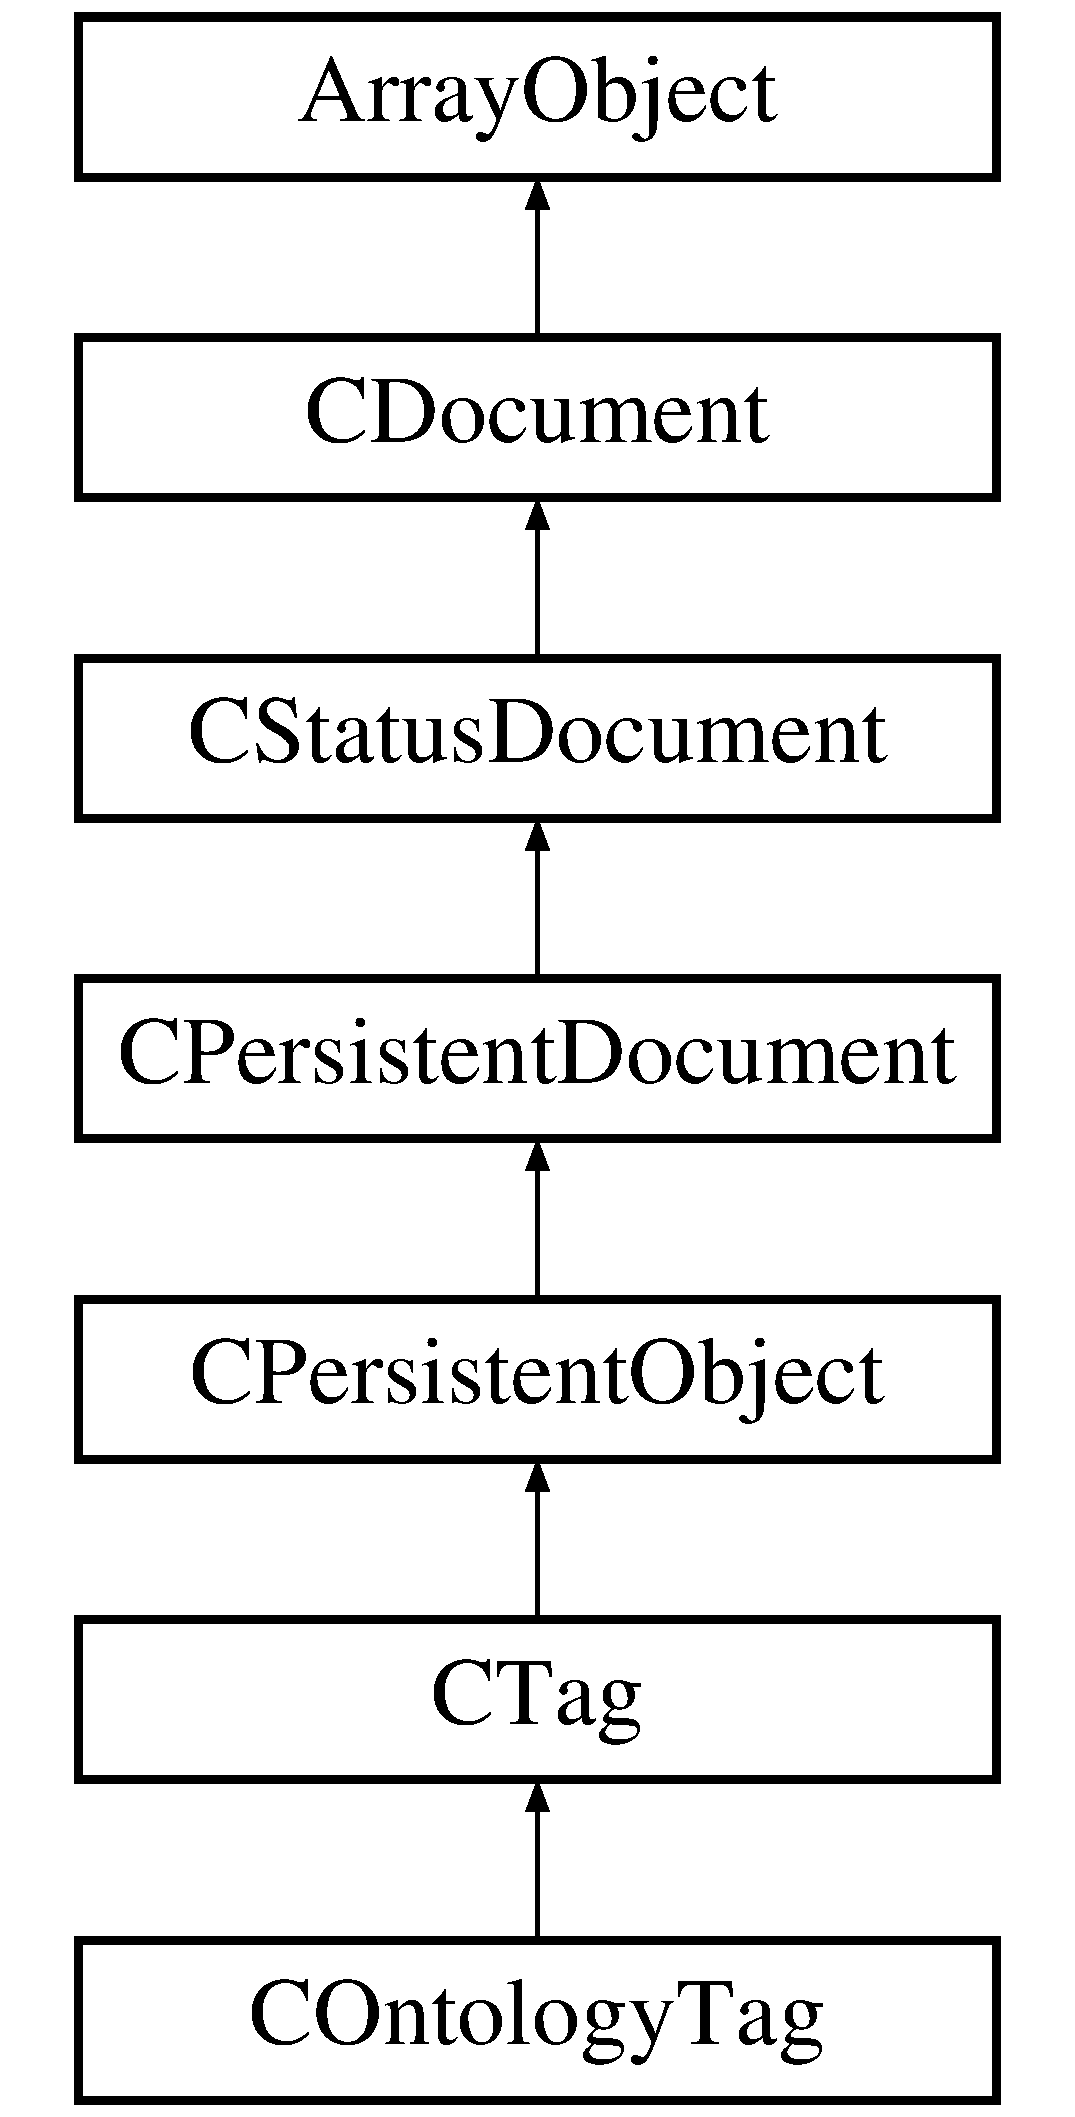
\includegraphics[height=7.000000cm]{class_c_ontology_tag}
\end{center}
\end{figure}
\subsection*{Public Member Functions}
\begin{DoxyCompactItemize}
\item 
\hyperlink{class_c_ontology_tag_a45c4c0a6da476d700c8197d77be016f8}{Push\-Item} (\$the\-Value)
\item 
\hyperlink{class_c_ontology_tag_a6f6ab6398a55f25e2860bac885f7f814}{Get\-Feature\-Vertex} ()
\item 
\hyperlink{class_c_ontology_tag_aa26d8df12c96f1018e3542303ba6ed1f}{Get\-Method\-Vertex} ()
\item 
\hyperlink{class_c_ontology_tag_acbbea165aff630988cb30c069b97dfc5}{Get\-Scale\-Vertex} ()
\item 
\hyperlink{class_c_ontology_tag_ae5aaf4673b9384c0bacbdc0b3cb2b1c8}{Update} (\hyperlink{class_c_connection}{C\-Connection} \$the\-Connection)
\item 
\hyperlink{class_c_ontology_tag_a878c491b0bb9f60c26c48a3797df15b8}{Replace} (\hyperlink{class_c_connection}{C\-Connection} \$the\-Connection)
\end{DoxyCompactItemize}
\subsection*{Static Public Member Functions}
\begin{DoxyCompactItemize}
\item 
static \hyperlink{class_c_ontology_tag_aba44e3b95b1e1830766f9647a2ea5f70}{Default\-Container\-Name} ()
\item 
static \hyperlink{class_c_ontology_tag_a58669fac5e450f687de2d4aad38bd4c4}{Resolve} (\hyperlink{class_c_connection}{C\-Connection} \$the\-Connection, \$the\-Identifier, \$do\-Throw=F\-A\-L\-S\-E)
\end{DoxyCompactItemize}
\subsection*{Protected Member Functions}
\begin{DoxyCompactItemize}
\item 
\hyperlink{class_c_ontology_tag_ad63039ab484008c15c69568d6bbf12eb}{\-\_\-index} (\hyperlink{class_c_connection}{C\-Connection} \$the\-Connection, \$the\-Modifiers)
\item 
\hyperlink{class_c_ontology_tag_a1d35d537264fffd4c7ba5ef79eeef6c0}{\-\_\-\-Preset} (\&\$the\-Offset, \&\$the\-Value)
\item 
\hyperlink{class_c_ontology_tag_a7f7edbf70627f225f4472010e80a3e52}{\-\_\-\-Preunset} (\&\$the\-Offset)
\item 
\hyperlink{class_c_ontology_tag_a3375cb63452f0b548940f3a64582cb3d}{\-\_\-\-Precommit\-Validate} (\&\$the\-Connection, \&\$the\-Modifiers)
\item 
\hyperlink{class_c_ontology_tag_a8d6a3cc0813c4b640a7a5927ba32daec}{\-\_\-\-Precommit\-Identify} (\&\$the\-Connection, \&\$the\-Modifiers)
\item 
\hyperlink{class_c_ontology_tag_a56757bb672c40d62798290c0c8bbdd5a}{\-\_\-\-Postcommit\-Related} (\&\$the\-Connection, \&\$the\-Modifiers)
\end{DoxyCompactItemize}
\subsection*{Additional Inherited Members}


\subsection{Member Function Documentation}
\hypertarget{class_c_ontology_tag_ad63039ab484008c15c69568d6bbf12eb}{\index{C\-Ontology\-Tag@{C\-Ontology\-Tag}!\-\_\-index@{\-\_\-index}}
\index{\-\_\-index@{\-\_\-index}!COntologyTag@{C\-Ontology\-Tag}}
\subsubsection[{\-\_\-index}]{\setlength{\rightskip}{0pt plus 5cm}C\-Ontology\-Tag\-::\-\_\-index (
\begin{DoxyParamCaption}
\item[{{\bf C\-Connection}}]{\$the\-Connection, }
\item[{}]{\$the\-Modifiers}
\end{DoxyParamCaption}
)\hspace{0.3cm}{\ttfamily [protected]}}}\label{class_c_ontology_tag_ad63039ab484008c15c69568d6bbf12eb}
\subparagraph*{Return the object's global unique identifier}

We override the parent method to handle the referenced objects\-: in this class the global identifier is the concatenation of all the referenced terms of the tag path, this method will take care of instantiating the necessary objects and building the global identifier.

This method is called by the \hyperlink{class_c_ontology_tag_a8d6a3cc0813c4b640a7a5927ba32daec}{\-\_\-\-Precommit\-Identify()} and expects all elements of the path to be object native identifiers.


\begin{DoxyParams}[1]{Parameters}
\hyperlink{class_c_connection}{C\-Connection} & {\em \$the\-Connection} & Server, database or container. \\
\hline
bitfield & {\em \$the\-Modifiers} & Commit options.\\
\hline
\end{DoxyParams}

\begin{DoxyExceptions}{Exceptions}
{\em Exception} & protected \\
\hline
\end{DoxyExceptions}
\begin{DoxyReturn}{Returns}
string$|$\-N\-U\-L\-L The object's global unique identifier.
\end{DoxyReturn}

\begin{DoxyExceptions}{Exceptions}
{\em Exception} & \\
\hline
\end{DoxyExceptions}
\begin{DoxySeeAlso}{See Also}
k\-T\-A\-G\-\_\-\-P\-A\-T\-H k\-T\-O\-K\-E\-N\-\_\-\-I\-N\-D\-E\-X\-\_\-\-S\-E\-P\-A\-R\-A\-T\-O\-R 
\end{DoxySeeAlso}
\hypertarget{class_c_ontology_tag_a56757bb672c40d62798290c0c8bbdd5a}{\index{C\-Ontology\-Tag@{C\-Ontology\-Tag}!\-\_\-\-Postcommit\-Related@{\-\_\-\-Postcommit\-Related}}
\index{\-\_\-\-Postcommit\-Related@{\-\_\-\-Postcommit\-Related}!COntologyTag@{C\-Ontology\-Tag}}
\subsubsection[{\-\_\-\-Postcommit\-Related}]{\setlength{\rightskip}{0pt plus 5cm}C\-Ontology\-Tag\-::\-\_\-\-Postcommit\-Related (
\begin{DoxyParamCaption}
\item[{\&}]{\$the\-Connection, }
\item[{\&}]{\$the\-Modifiers}
\end{DoxyParamCaption}
)\hspace{0.3cm}{\ttfamily [protected]}}}\label{class_c_ontology_tag_a56757bb672c40d62798290c0c8bbdd5a}
\subparagraph*{Update related objects after committing}

In this class we reference this tag from terms related to nodes used as features, methods or scales. Depending on the value of the following flags\-:


\begin{DoxyItemize}
\item {\ttfamily \hyperlink{}{k\-S\-W\-I\-T\-C\-H\-\_\-k\-T\-A\-G\-\_\-\-F\-E\-A\-T\-U\-R\-E\-S}}\-: {\itshape Feature node reference}. This switch manages references to the current tag from terms referred by feature nodes, or the first node in the path. The reference is in the \hyperlink{}{k\-T\-A\-G\-\_\-\-F\-E\-A\-T\-U\-R\-E\-S} of the referenced term. 
\begin{DoxyItemize}
\item {\ttfamily 0x2}\-: {\itshape Keep count of references}. This means that the \hyperlink{}{k\-T\-A\-G\-\_\-\-F\-E\-A\-T\-U\-R\-E\-S} attribute of the term will be incremented when the tag is inserted, or decremented when deleted. 
\item {\ttfamily 0x3}\-: {\itshape Keep list of references}. This means that a reference to the current object will be added to the \hyperlink{}{k\-T\-A\-G\-\_\-\-F\-E\-A\-T\-U\-R\-E\-S} attribute of the term when the current object is inserted, and removed when the object is deleted. 
\item {\ttfamily 0x0} {\itshape or other}\-: {\itshape Don't handle this information}. This means that the term's \hyperlink{}{k\-T\-A\-G\-\_\-\-F\-E\-A\-T\-U\-R\-E\-S} attribute will not be handled. 
\end{DoxyItemize}
\item {\ttfamily \hyperlink{}{k\-S\-W\-I\-T\-C\-H\-\_\-k\-T\-A\-G\-\_\-\-M\-E\-T\-H\-O\-D\-S}}\-: {\itshape Method node reference}. This switch manages references to the current tag from terms referred by method nodes, or all nodes between the first and last nodes in the path. The reference is in the \hyperlink{}{k\-S\-W\-I\-T\-C\-H\-\_\-k\-T\-A\-G\-\_\-\-M\-E\-T\-H\-O\-D\-S} of the referenced term. 
\begin{DoxyItemize}
\item {\ttfamily 0x2}\-: {\itshape Keep count of references}. This means that the \hyperlink{}{k\-S\-W\-I\-T\-C\-H\-\_\-k\-T\-A\-G\-\_\-\-M\-E\-T\-H\-O\-D\-S} attribute of the term will be incremented when the tag is inserted, or decremented when deleted. 
\item {\ttfamily 0x3}\-: {\itshape Keep list of references}. This means that a reference to the current object will be added to the \hyperlink{}{k\-S\-W\-I\-T\-C\-H\-\_\-k\-T\-A\-G\-\_\-\-M\-E\-T\-H\-O\-D\-S} attribute of the term when the current object is inserted, and removed when the object is deleted. 
\item {\ttfamily 0x0} {\itshape or other}\-: {\itshape Don't handle this information}. This means that the term's \hyperlink{}{k\-S\-W\-I\-T\-C\-H\-\_\-k\-T\-A\-G\-\_\-\-M\-E\-T\-H\-O\-D\-S} attribute will not be handled. 
\end{DoxyItemize}
\item {\ttfamily \hyperlink{}{k\-S\-W\-I\-T\-C\-H\-\_\-k\-T\-A\-G\-\_\-\-S\-C\-A\-L\-E\-S}}\-: {\itshape Scale node reference}. This switch manages references to the current tag from terms referred by scale nodes, or the last node in the path. The reference is in the \hyperlink{}{k\-T\-A\-G\-\_\-\-S\-C\-A\-L\-E\-S} of the referenced term. 
\begin{DoxyItemize}
\item {\ttfamily 0x2}\-: {\itshape Keep count of references}. This means that the \hyperlink{}{k\-T\-A\-G\-\_\-\-S\-C\-A\-L\-E\-S} attribute of the term will be incremented when the tag is inserted, or decremented when deleted. 
\item {\ttfamily 0x3}\-: {\itshape Keep list of references}. This means that a reference to the current object will be added to the \hyperlink{}{k\-T\-A\-G\-\_\-\-S\-C\-A\-L\-E\-S} attribute of the term when the current object is inserted, and removed when the object is deleted. 
\item {\ttfamily 0x0} {\itshape or other}\-: {\itshape Don't handle this information}. This means that the term's \hyperlink{}{k\-T\-A\-G\-\_\-\-S\-C\-A\-L\-E\-S} attribute will not be handled. 
\end{DoxyItemize}
\end{DoxyItemize}

Note that you should provide either a database connection or the {\itshape term} container to this method in order to make it work!

We only handle vertex elements, we do not refer predicate terms.


\begin{DoxyParams}[1]{Parameters}
reference & {\em \&\$the\-Connection} & Server, database or container. \\
\hline
reference & {\em \&\$the\-Modifiers} & Commit options.\\
\hline
\end{DoxyParams}
protected

\begin{DoxySeeAlso}{See Also}
k\-S\-W\-I\-T\-C\-H\-\_\-k\-T\-A\-G\-\_\-\-F\-E\-A\-T\-U\-R\-E\-S, k\-S\-W\-I\-T\-C\-H\-\_\-k\-T\-A\-G\-\_\-\-M\-E\-T\-H\-O\-D\-S, k\-S\-W\-I\-T\-C\-H\-\_\-k\-T\-A\-G\-\_\-\-S\-C\-A\-L\-E\-S 

k\-T\-A\-G\-\_\-\-F\-E\-A\-T\-U\-R\-E\-S, k\-T\-A\-G\-\_\-\-M\-E\-T\-H\-O\-D\-S, k\-T\-A\-G\-\_\-\-S\-C\-A\-L\-E\-S 

k\-F\-L\-A\-G\-\_\-\-P\-E\-R\-S\-I\-S\-T\-\_\-\-I\-N\-S\-E\-R\-T k\-F\-L\-A\-G\-\_\-\-P\-E\-R\-S\-I\-S\-T\-\_\-\-R\-E\-P\-L\-A\-C\-E k\-F\-L\-A\-G\-\_\-\-P\-E\-R\-S\-I\-S\-T\-\_\-\-D\-E\-L\-E\-T\-E 
\end{DoxySeeAlso}
\hypertarget{class_c_ontology_tag_a8d6a3cc0813c4b640a7a5927ba32daec}{\index{C\-Ontology\-Tag@{C\-Ontology\-Tag}!\-\_\-\-Precommit\-Identify@{\-\_\-\-Precommit\-Identify}}
\index{\-\_\-\-Precommit\-Identify@{\-\_\-\-Precommit\-Identify}!COntologyTag@{C\-Ontology\-Tag}}
\subsubsection[{\-\_\-\-Precommit\-Identify}]{\setlength{\rightskip}{0pt plus 5cm}C\-Ontology\-Tag\-::\-\_\-\-Precommit\-Identify (
\begin{DoxyParamCaption}
\item[{\&}]{\$the\-Connection, }
\item[{\&}]{\$the\-Modifiers}
\end{DoxyParamCaption}
)\hspace{0.3cm}{\ttfamily [protected]}}}\label{class_c_ontology_tag_a8d6a3cc0813c4b640a7a5927ba32daec}
\subparagraph*{Determine the identifiers before committing}

This method will use the result of the \hyperlink{class_c_ontology_tag_ad63039ab484008c15c69568d6bbf12eb}{\-\_\-index()} method to set the global identifier, \hyperlink{}{k\-T\-A\-G\-\_\-\-G\-I\-D}; the same value will be hashed and constitute the unique identifier, \hyperlink{}{k\-T\-A\-G\-\_\-\-U\-I\-D}, while the native identifier, \hyperlink{}{k\-T\-A\-G\-\_\-\-N\-I\-D}, will be set by the sequence number \hyperlink{}{k\-S\-E\-Q\-U\-E\-N\-C\-E\-\_\-\-K\-E\-Y\-\_\-\-T\-A\-G}.

The parent method will then be called, which will ignore the global and native identifiers, since they will have been set here.


\begin{DoxyParams}[1]{Parameters}
reference & {\em \&\$the\-Connection} & Server, database or container. \\
\hline
reference & {\em \&\$the\-Modifiers} & Commit options.\\
\hline
\end{DoxyParams}
protected \begin{DoxyReturn}{Returns}
mixed
\end{DoxyReturn}

\begin{DoxyExceptions}{Exceptions}
{\em Exception} & \hyperlink{class_c_status_document_ab7d96fd4588cf7d5432fc65a1d1fb076}{\-\_\-\-Is\-Committed()}  \hyperlink{class_c_ontology_tag_ad63039ab484008c15c69568d6bbf12eb}{\-\_\-index()}\\
\hline
\end{DoxyExceptions}
\begin{DoxySeeAlso}{See Also}
k\-S\-E\-Q\-U\-E\-N\-C\-E\-\_\-\-K\-E\-Y\-\_\-\-T\-A\-G 

k\-T\-A\-G\-\_\-\-N\-I\-D k\-T\-A\-G\-\_\-\-G\-I\-D k\-T\-A\-G\-\_\-\-U\-I\-D 

k\-F\-L\-A\-G\-\_\-\-P\-E\-R\-S\-I\-S\-T\-\_\-\-I\-N\-S\-E\-R\-T k\-F\-L\-A\-G\-\_\-\-P\-E\-R\-S\-I\-S\-T\-\_\-\-R\-E\-P\-L\-A\-C\-E 
\end{DoxySeeAlso}
\hypertarget{class_c_ontology_tag_a3375cb63452f0b548940f3a64582cb3d}{\index{C\-Ontology\-Tag@{C\-Ontology\-Tag}!\-\_\-\-Precommit\-Validate@{\-\_\-\-Precommit\-Validate}}
\index{\-\_\-\-Precommit\-Validate@{\-\_\-\-Precommit\-Validate}!COntologyTag@{C\-Ontology\-Tag}}
\subsubsection[{\-\_\-\-Precommit\-Validate}]{\setlength{\rightskip}{0pt plus 5cm}C\-Ontology\-Tag\-::\-\_\-\-Precommit\-Validate (
\begin{DoxyParamCaption}
\item[{\&}]{\$the\-Connection, }
\item[{\&}]{\$the\-Modifiers}
\end{DoxyParamCaption}
)\hspace{0.3cm}{\ttfamily [protected]}}}\label{class_c_ontology_tag_a3375cb63452f0b548940f3a64582cb3d}
\subparagraph*{Validate the object before committing}

In this class we check if the type is set, if that is not the case, the method will raise an exception.


\begin{DoxyParams}[1]{Parameters}
reference & {\em \&\$the\-Connection} & Server, database or container. \\
\hline
reference & {\em \&\$the\-Modifiers} & Commit options.\\
\hline
\end{DoxyParams}
protected \begin{DoxyReturn}{Returns}
mixed
\end{DoxyReturn}

\begin{DoxyExceptions}{Exceptions}
{\em Exception} & \\
\hline
\end{DoxyExceptions}
\begin{DoxySeeAlso}{See Also}
k\-T\-A\-G\-\_\-\-T\-Y\-P\-E 
\end{DoxySeeAlso}
\hypertarget{class_c_ontology_tag_a1d35d537264fffd4c7ba5ef79eeef6c0}{\index{C\-Ontology\-Tag@{C\-Ontology\-Tag}!\-\_\-\-Preset@{\-\_\-\-Preset}}
\index{\-\_\-\-Preset@{\-\_\-\-Preset}!COntologyTag@{C\-Ontology\-Tag}}
\subsubsection[{\-\_\-\-Preset}]{\setlength{\rightskip}{0pt plus 5cm}C\-Ontology\-Tag\-::\-\_\-\-Preset (
\begin{DoxyParamCaption}
\item[{\&}]{\$the\-Offset, }
\item[{\&}]{\$the\-Value}
\end{DoxyParamCaption}
)\hspace{0.3cm}{\ttfamily [protected]}}}\label{class_c_ontology_tag_a1d35d537264fffd4c7ba5ef79eeef6c0}
\subparagraph*{Handle offset before setting it}

In this class we lock the \hyperlink{}{k\-T\-A\-G\-\_\-\-P\-A\-T\-H} attribute if the object is committed.


\begin{DoxyParams}[1]{Parameters}
reference & {\em \&\$the\-Offset} & Offset. \\
\hline
reference & {\em \&\$the\-Value} & Value to set at offset.\\
\hline
\end{DoxyParams}
protected


\begin{DoxyExceptions}{Exceptions}
{\em Exception} & \hyperlink{class_c_status_document_ab7d96fd4588cf7d5432fc65a1d1fb076}{\-\_\-\-Is\-Committed()}\\
\hline
\end{DoxyExceptions}
\begin{DoxySeeAlso}{See Also}
k\-T\-A\-G\-\_\-\-P\-A\-T\-H 
\end{DoxySeeAlso}
\hypertarget{class_c_ontology_tag_a7f7edbf70627f225f4472010e80a3e52}{\index{C\-Ontology\-Tag@{C\-Ontology\-Tag}!\-\_\-\-Preunset@{\-\_\-\-Preunset}}
\index{\-\_\-\-Preunset@{\-\_\-\-Preunset}!COntologyTag@{C\-Ontology\-Tag}}
\subsubsection[{\-\_\-\-Preunset}]{\setlength{\rightskip}{0pt plus 5cm}C\-Ontology\-Tag\-::\-\_\-\-Preunset (
\begin{DoxyParamCaption}
\item[{\&}]{\$the\-Offset}
\end{DoxyParamCaption}
)\hspace{0.3cm}{\ttfamily [protected]}}}\label{class_c_ontology_tag_a7f7edbf70627f225f4472010e80a3e52}
\subparagraph*{Handle offset before unsetting it}

In this class we lock the \hyperlink{}{k\-T\-A\-G\-\_\-\-P\-A\-T\-H} attribute if the object is committed and the \hyperlink{}{k\-T\-A\-G\-\_\-\-U\-I\-D} in all cases.


\begin{DoxyParams}[1]{Parameters}
reference & {\em \&\$the\-Offset} & Offset.\\
\hline
\end{DoxyParams}
protected


\begin{DoxyExceptions}{Exceptions}
{\em Exception} & \hyperlink{class_c_status_document_ab7d96fd4588cf7d5432fc65a1d1fb076}{\-\_\-\-Is\-Committed()}\\
\hline
\end{DoxyExceptions}
\begin{DoxySeeAlso}{See Also}
k\-T\-A\-G\-\_\-\-P\-A\-T\-H 
\end{DoxySeeAlso}
\hypertarget{class_c_ontology_tag_aba44e3b95b1e1830766f9647a2ea5f70}{\index{C\-Ontology\-Tag@{C\-Ontology\-Tag}!Default\-Container\-Name@{Default\-Container\-Name}}
\index{Default\-Container\-Name@{Default\-Container\-Name}!COntologyTag@{C\-Ontology\-Tag}}
\subsubsection[{Default\-Container\-Name}]{\setlength{\rightskip}{0pt plus 5cm}static C\-Ontology\-Tag\-::\-Default\-Container\-Name (
\begin{DoxyParamCaption}
{}
\end{DoxyParamCaption}
)\hspace{0.3cm}{\ttfamily [static]}}}\label{class_c_ontology_tag_aba44e3b95b1e1830766f9647a2ea5f70}
\subparagraph*{Return the default nodes container name}

This class uses the \hyperlink{}{k\-C\-O\-N\-T\-A\-I\-N\-E\-R\-\_\-\-T\-A\-G\-\_\-\-N\-A\-M\-E} default name.

\begin{DoxyReturn}{Returns}
string The default container name.
\end{DoxyReturn}

\begin{DoxyExceptions}{Exceptions}
{\em Exception} & \\
\hline
\end{DoxyExceptions}
\begin{DoxySeeAlso}{See Also}
k\-C\-O\-N\-T\-A\-I\-N\-E\-R\-\_\-\-T\-A\-G\-\_\-\-N\-A\-M\-E 
\end{DoxySeeAlso}
\hypertarget{class_c_ontology_tag_a6f6ab6398a55f25e2860bac885f7f814}{\index{C\-Ontology\-Tag@{C\-Ontology\-Tag}!Get\-Feature\-Vertex@{Get\-Feature\-Vertex}}
\index{Get\-Feature\-Vertex@{Get\-Feature\-Vertex}!COntologyTag@{C\-Ontology\-Tag}}
\subsubsection[{Get\-Feature\-Vertex}]{\setlength{\rightskip}{0pt plus 5cm}C\-Ontology\-Tag\-::\-Get\-Feature\-Vertex (
\begin{DoxyParamCaption}
{}
\end{DoxyParamCaption}
)}}\label{class_c_ontology_tag_a6f6ab6398a55f25e2860bac885f7f814}
\subparagraph*{Return trait term}

This method will return the current tag's feature term, if present, or {\ttfamily N\-U\-L\-L}.

The feature vertex is the first element of the path, it refers the ontology term that represents the feature or trait the current object is tagging.

public \begin{DoxyReturn}{Returns}
mixed First element of the terms list, or {\ttfamily N\-U\-L\-L}.
\end{DoxyReturn}
\begin{DoxySeeAlso}{See Also}
k\-T\-A\-G\-\_\-\-P\-A\-T\-H 
\end{DoxySeeAlso}
\hypertarget{class_c_ontology_tag_aa26d8df12c96f1018e3542303ba6ed1f}{\index{C\-Ontology\-Tag@{C\-Ontology\-Tag}!Get\-Method\-Vertex@{Get\-Method\-Vertex}}
\index{Get\-Method\-Vertex@{Get\-Method\-Vertex}!COntologyTag@{C\-Ontology\-Tag}}
\subsubsection[{Get\-Method\-Vertex}]{\setlength{\rightskip}{0pt plus 5cm}C\-Ontology\-Tag\-::\-Get\-Method\-Vertex (
\begin{DoxyParamCaption}
{}
\end{DoxyParamCaption}
)}}\label{class_c_ontology_tag_aa26d8df12c96f1018e3542303ba6ed1f}
\subparagraph*{Return method terms}

This method will return the current tag's list of method terms, if present, or {\ttfamily N\-U\-L\-L}.

The method vertex is the any odd element of the path that is neither the first nor the last, it represents the pipeline of modifiers applied to the feature vertex.

The method will return an array if at least one method is present.

Note that there must be at least 5 elements in the path to have one method.

public \begin{DoxyReturn}{Returns}
mixed List of method nodes, or {\ttfamily N\-U\-L\-L}.
\end{DoxyReturn}
\begin{DoxySeeAlso}{See Also}
k\-T\-A\-G\-\_\-\-P\-A\-T\-H 
\end{DoxySeeAlso}
\hypertarget{class_c_ontology_tag_acbbea165aff630988cb30c069b97dfc5}{\index{C\-Ontology\-Tag@{C\-Ontology\-Tag}!Get\-Scale\-Vertex@{Get\-Scale\-Vertex}}
\index{Get\-Scale\-Vertex@{Get\-Scale\-Vertex}!COntologyTag@{C\-Ontology\-Tag}}
\subsubsection[{Get\-Scale\-Vertex}]{\setlength{\rightskip}{0pt plus 5cm}C\-Ontology\-Tag\-::\-Get\-Scale\-Vertex (
\begin{DoxyParamCaption}
{}
\end{DoxyParamCaption}
)}}\label{class_c_ontology_tag_acbbea165aff630988cb30c069b97dfc5}
\subparagraph*{Return scale term}

This method will return the current tag's scale term, if present, or {\ttfamily N\-U\-L\-L}.

The scale vertex is the last element of the path, it refers the ontology term that represents the scale or unit the current object is tagging.

Note that if the tag contains only one vertex, that will be both a feature and a scale.

public \begin{DoxyReturn}{Returns}
mixed Last element of the terms list, or {\ttfamily N\-U\-L\-L}.
\end{DoxyReturn}
\begin{DoxySeeAlso}{See Also}
k\-T\-A\-G\-\_\-\-P\-A\-T\-H 
\end{DoxySeeAlso}
\hypertarget{class_c_ontology_tag_a45c4c0a6da476d700c8197d77be016f8}{\index{C\-Ontology\-Tag@{C\-Ontology\-Tag}!Push\-Item@{Push\-Item}}
\index{Push\-Item@{Push\-Item}!COntologyTag@{C\-Ontology\-Tag}}
\subsubsection[{Push\-Item}]{\setlength{\rightskip}{0pt plus 5cm}C\-Ontology\-Tag\-::\-Push\-Item (
\begin{DoxyParamCaption}
\item[{}]{\$the\-Value}
\end{DoxyParamCaption}
)}}\label{class_c_ontology_tag_a45c4c0a6da476d700c8197d77be016f8}
\subparagraph*{Append to path}

We overload the parent method to implement the following rules\-:


\begin{DoxyItemize}
\item All elements of the path must be \hyperlink{class_c_ontology_term}{C\-Ontology\-Term} instance references. 
\item Odd elements of the path are graph vertices and can be provided as \hyperlink{class_c_ontology_node}{C\-Ontology\-Node} instances\-: 
\begin{DoxyItemize}
\item \hyperlink{class_c_ontology_node}{C\-Ontology\-Node} instances will be converted into their \hyperlink{}{k\-T\-A\-G\-\_\-\-T\-E\-R\-M} property. 
\item {\ttfamily Integer} values will {\itshape not} be interpreted as node references, since there is no way to resolve them. 
\item If the first element of the path is an \hyperlink{class_c_ontology_node}{C\-Ontology\-Node} instance, the latter must have its \hyperlink{}{k\-T\-A\-G\-\_\-\-K\-I\-N\-D} attribute set to \hyperlink{}{k\-K\-I\-N\-D\-\_\-\-F\-E\-A\-T\-U\-R\-E}. 
\item If the last element of the path is an \hyperlink{class_c_ontology_node}{C\-Ontology\-Node} instance, the latter must have its \hyperlink{}{k\-T\-A\-G\-\_\-\-K\-I\-N\-D} attribute set to \hyperlink{}{k\-K\-I\-N\-D\-\_\-\-S\-C\-A\-L\-E}. 
\end{DoxyItemize}
\item \{link \hyperlink{class_c_ontology_term}{C\-Ontology\-Term}\} instances will be accepted in any position. 
\item \{link \hyperlink{class_c_ontology_term}{C\-Ontology\-Term}\} instances must have their \hyperlink{}{k\-T\-A\-G\-\_\-\-N\-I\-D} attribute. 
\item Any other data type will be interpreted as the term's \hyperlink{}{k\-T\-A\-G\-\_\-\-N\-I\-D} and no verification will be performed. 
\end{DoxyItemize}

In addition, the following attributes will be copied into the current object\-:


\begin{DoxyItemize}
\item {\ttfamily \hyperlink{}{k\-T\-A\-G\-\_\-\-S\-Y\-N\-O\-N\-Y\-M\-S}}\-: From the eventual feature term. 
\item {\ttfamily \hyperlink{}{k\-T\-A\-G\-\_\-\-T\-Y\-P\-E}}\-: From the eventual scale vertex. 
\item {\ttfamily \hyperlink{}{k\-T\-A\-G\-\_\-\-I\-N\-P\-U\-T}}\-: From the eventual scale vertex. 
\item {\ttfamily \hyperlink{}{k\-T\-A\-G\-\_\-\-P\-A\-T\-T\-E\-R\-N}}\-: From the eventual scale vertex. 
\item {\ttfamily \hyperlink{}{k\-T\-A\-G\-\_\-\-L\-E\-N\-G\-T\-H}}\-: From the eventual scale vertex. 
\item {\ttfamily \hyperlink{}{k\-T\-A\-G\-\_\-\-M\-I\-N\-\_\-\-V\-A\-L}}\-: From the eventual scale vertex. 
\item {\ttfamily \hyperlink{}{k\-T\-A\-G\-\_\-\-M\-A\-X\-\_\-\-V\-A\-L}}\-: From the eventual scale vertex. 
\item {\ttfamily \hyperlink{}{k\-T\-A\-G\-\_\-\-E\-X\-A\-M\-P\-L\-E\-S}}\-: From the eventual scale vertex. 
\end{DoxyItemize}


\begin{DoxyParams}[1]{Parameters}
mixed & {\em \$the\-Value} & Value to append.\\
\hline
\end{DoxyParams}
public \begin{DoxyReturn}{Returns}
integer Number of items in the list.
\end{DoxyReturn}
\hyperlink{class_c_persistent_object_aaddbaf409e7cab172ce6a92631d9ae45}{\-\_\-\-Assert\-Class()}

\begin{DoxySeeAlso}{See Also}
k\-T\-A\-G\-\_\-\-P\-A\-T\-H 
\end{DoxySeeAlso}
\hypertarget{class_c_ontology_tag_a878c491b0bb9f60c26c48a3797df15b8}{\index{C\-Ontology\-Tag@{C\-Ontology\-Tag}!Replace@{Replace}}
\index{Replace@{Replace}!COntologyTag@{C\-Ontology\-Tag}}
\subsubsection[{Replace}]{\setlength{\rightskip}{0pt plus 5cm}C\-Ontology\-Tag\-::\-Replace (
\begin{DoxyParamCaption}
\item[{{\bf C\-Connection}}]{\$the\-Connection}
\end{DoxyParamCaption}
)}}\label{class_c_ontology_tag_a878c491b0bb9f60c26c48a3797df15b8}
\subparagraph*{Replace the object into a container}

We overload this method to raise an exception\-: objects of this class can only be inserted, after this one can only modify their attributes using the modification interface provided by container objects.

In this class we prevent replacing a committed object and allow inserting a non committed object.


\begin{DoxyParams}[1]{Parameters}
\hyperlink{class_c_connection}{C\-Connection} & {\em \$the\-Connection} & Server, database or container.\\
\hline
\end{DoxyParams}
public \begin{DoxyReturn}{Returns}
mixed The object's native identifier. 
\end{DoxyReturn}
\hypertarget{class_c_ontology_tag_a58669fac5e450f687de2d4aad38bd4c4}{\index{C\-Ontology\-Tag@{C\-Ontology\-Tag}!Resolve@{Resolve}}
\index{Resolve@{Resolve}!COntologyTag@{C\-Ontology\-Tag}}
\subsubsection[{Resolve}]{\setlength{\rightskip}{0pt plus 5cm}static C\-Ontology\-Tag\-::\-Resolve (
\begin{DoxyParamCaption}
\item[{{\bf C\-Connection}}]{\$the\-Connection, }
\item[{}]{\$the\-Identifier, }
\item[{}]{\$do\-Throw = {\ttfamily FALSE}}
\end{DoxyParamCaption}
)\hspace{0.3cm}{\ttfamily [static]}}}\label{class_c_ontology_tag_a58669fac5e450f687de2d4aad38bd4c4}
\subparagraph*{Resolve a tag}

This method can be used to retrieve an existing tag by identifier, or retrieve all tags matching a term.

The method accepts the following parameters\-:


\begin{DoxyItemize}
\item {\ttfamily \$the\-Connection}\-: This parameter represents the connection from which the tags container must be resolved. Note that this method might need to resolve the terms container, so provide at least a database. 
\item {\ttfamily \$the\-Identifier}\-: This parameter represents the identifier to be resolved\-: 
\begin{DoxyItemize}
\item {\ttfamily integer}\-: In this case the method assumes that the parameter represents the tag identifier\-: it will attempt to retrieve the tag, if it is not found, the method will return {\ttfamily N\-U\-L\-L}. 
\item {\ttfamily array}\-: In this case the method assumes the array is the tag path, \hyperlink{}{k\-T\-A\-G\-\_\-\-P\-A\-T\-H}, it will attempt to convert it into the tag \hyperlink{}{k\-T\-A\-G\-\_\-\-U\-I\-D} and locate it. 
\item {\itshape other}\-: Any other type will be interpreted as the tag's global identifier\-: the method will return the matching tag or {\ttfamily N\-U\-L\-L}. 
\end{DoxyItemize}
\item {\ttfamily \$do\-Throw}\-: If {\ttfamily T\-R\-U\-E}, any failure to resolve the tag will raise an exception. 
\end{DoxyItemize}

The method will return an instance of this class, or {\ttfamily N\-U\-L\-L}, if the identifier was not resolved.


\begin{DoxyParams}[1]{Parameters}
\hyperlink{class_c_connection}{C\-Connection} & {\em \$the\-Connection} & Server, database or container. \\
\hline
mixed & {\em \$the\-Identifier} & Identifier to be resolved. \\
\hline
boolean & {\em \$do\-Throw} & If {\ttfamily T\-R\-U\-E} raise an exception.\\
\hline
\end{DoxyParams}
\begin{DoxyReturn}{Returns}
\hyperlink{class_c_ontology_term}{C\-Ontology\-Term} Found tag or {\ttfamily N\-U\-L\-L}.
\end{DoxyReturn}

\begin{DoxyExceptions}{Exceptions}
{\em Exception} & \\
\hline
\end{DoxyExceptions}
\hypertarget{class_c_ontology_tag_ae5aaf4673b9384c0bacbdc0b3cb2b1c8}{\index{C\-Ontology\-Tag@{C\-Ontology\-Tag}!Update@{Update}}
\index{Update@{Update}!COntologyTag@{C\-Ontology\-Tag}}
\subsubsection[{Update}]{\setlength{\rightskip}{0pt plus 5cm}C\-Ontology\-Tag\-::\-Update (
\begin{DoxyParamCaption}
\item[{{\bf C\-Connection}}]{\$the\-Connection}
\end{DoxyParamCaption}
)}}\label{class_c_ontology_tag_ae5aaf4673b9384c0bacbdc0b3cb2b1c8}
\subparagraph*{Update the object in a container}

We overload this method to raise an exception\-: objects of this class can only be inserted, after this one can only modify their attributes using the modification interface provided by container objects.


\begin{DoxyParams}[1]{Parameters}
\hyperlink{class_c_connection}{C\-Connection} & {\em \$the\-Connection} & Server, database or container.\\
\hline
\end{DoxyParams}
public


\begin{DoxyExceptions}{Exceptions}
{\em Exception} & \\
\hline
\end{DoxyExceptions}


The documentation for this class was generated from the following file\-:\begin{DoxyCompactItemize}
\item 
/\-Library/\-Web\-Server/\-Library/\-P\-H\-P\-Wrapper/classes/C\-Ontology\-Tag.\-php\end{DoxyCompactItemize}

\hypertarget{class_c_ontology_term}{\section{C\-Ontology\-Term Class Reference}
\label{class_c_ontology_term}\index{C\-Ontology\-Term@{C\-Ontology\-Term}}
}
Inheritance diagram for C\-Ontology\-Term\-:\begin{figure}[H]
\begin{center}
\leavevmode
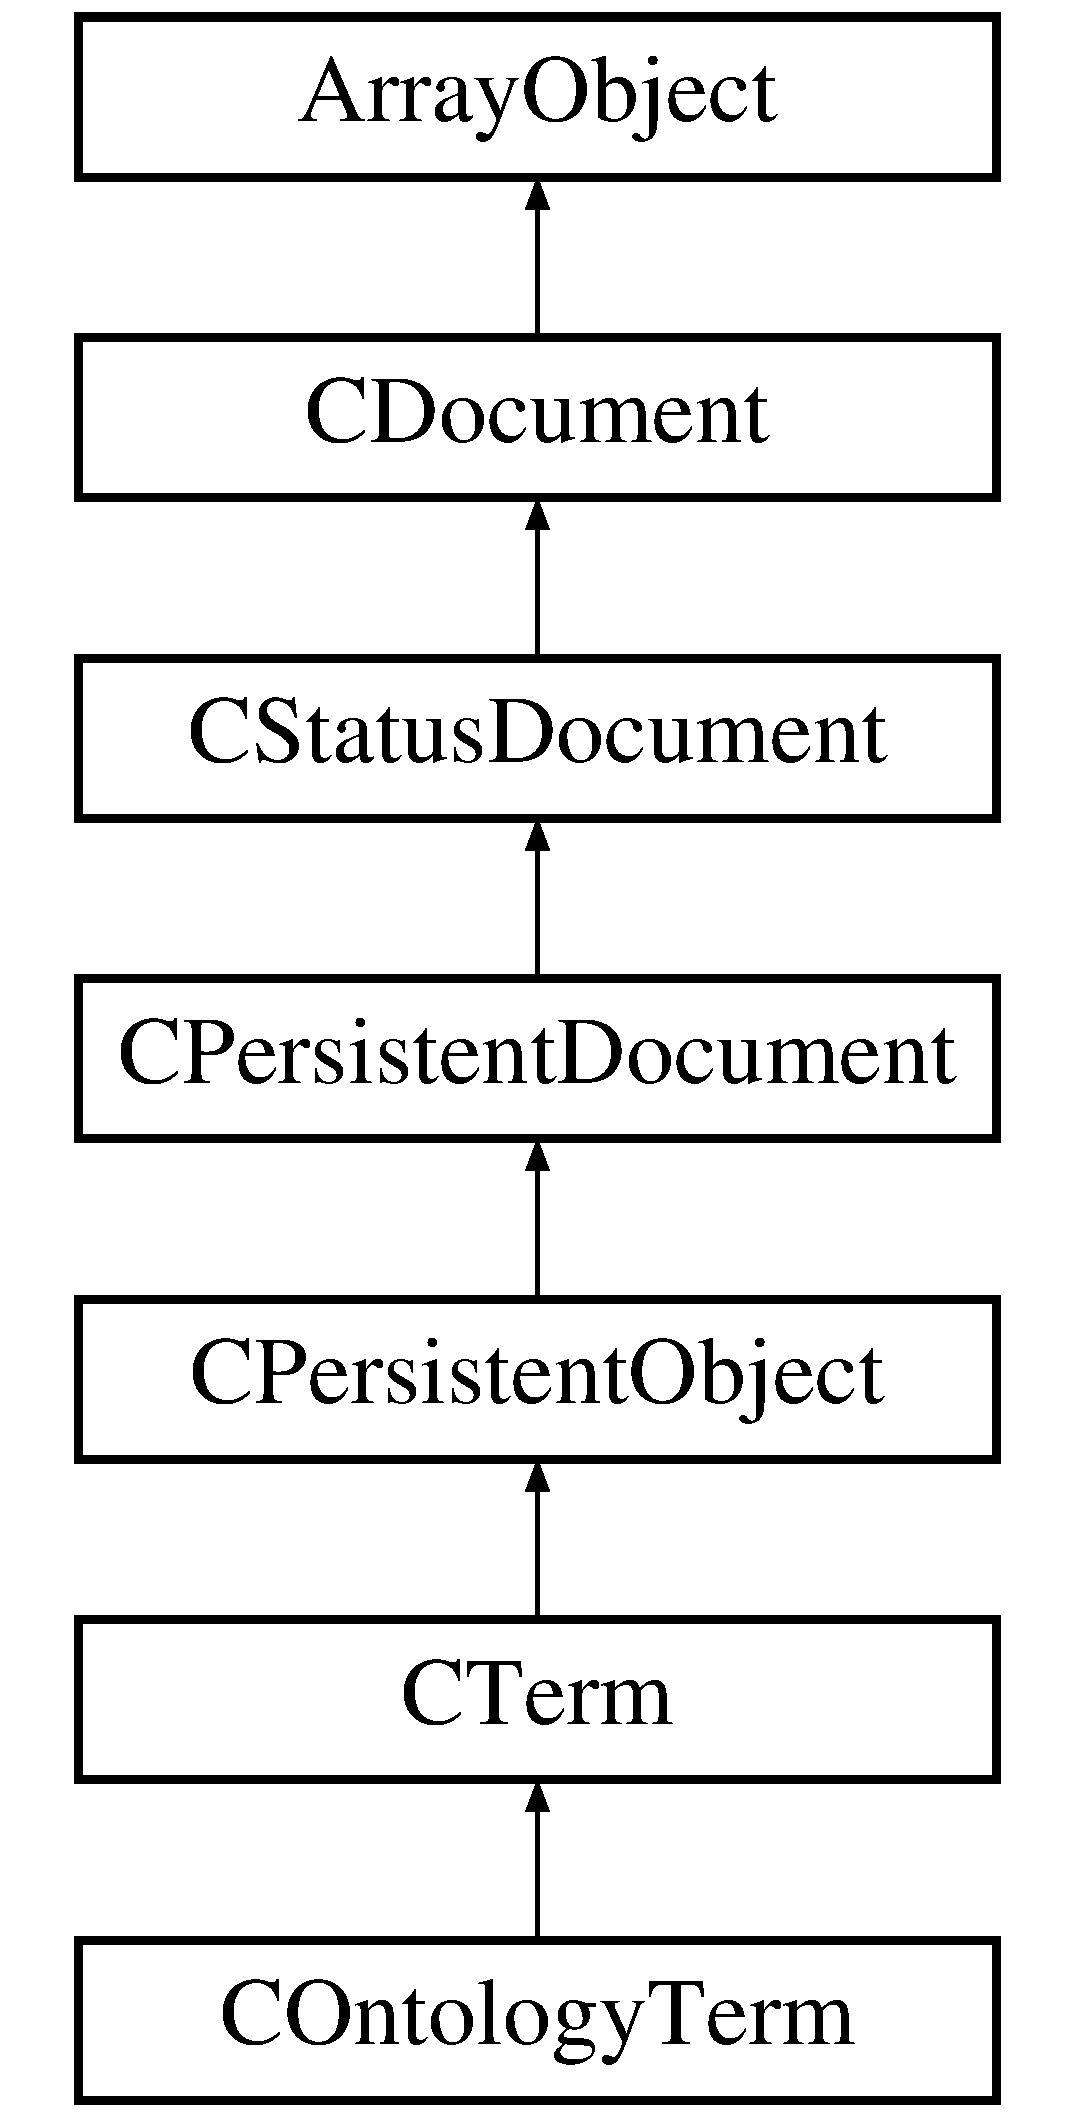
\includegraphics[height=7.000000cm]{class_c_ontology_term}
\end{center}
\end{figure}
\subsection*{Public Member Functions}
\begin{DoxyCompactItemize}
\item 
\hyperlink{class_c_ontology_term_af016ba966a7b3c9ce30724d0a9394af2}{Features} ()
\item 
\hyperlink{class_c_ontology_term_ae6beb36dde46c78f136e923c6dda99d9}{Methods} ()
\item 
\hyperlink{class_c_ontology_term_a0885898fdebb262a7ae71ec010249d46}{Scales} ()
\item 
\hyperlink{class_c_ontology_term_a31fa356129d058361b7cdd88924b6c7d}{Load\-Namespace} (\hyperlink{class_c_connection}{C\-Connection} \$the\-Connection, \$do\-Reload=F\-A\-L\-S\-E)
\item 
\hyperlink{class_c_ontology_term_a36c2ab4ffdde63d0ca51734437faaa35}{Load\-Term} (\hyperlink{class_c_connection}{C\-Connection} \$the\-Connection, \$do\-Reload=F\-A\-L\-S\-E)
\item 
\hyperlink{class_c_ontology_term_ac39334977998a1e11c0e277eac4cef5c}{Update} (\hyperlink{class_c_connection}{C\-Connection} \$the\-Connection)
\item 
\hyperlink{class_c_ontology_term_ac1257616ac8626822f410bd858ce767c}{Replace} (\hyperlink{class_c_connection}{C\-Connection} \$the\-Connection)
\end{DoxyCompactItemize}
\subsection*{Static Public Member Functions}
\begin{DoxyCompactItemize}
\item 
static \hyperlink{class_c_ontology_term_ab4c98ee0a638974d6c422fcb9df31471}{Handle\-Label} (\hyperlink{class_c_connection}{C\-Connection} \$the\-Connection, \$the\-Identifier, \$the\-Language=N\-U\-L\-L, \$the\-Value=N\-U\-L\-L)
\item 
static \hyperlink{class_c_ontology_term_a41ecd119648036a63b083f1dad064554}{Default\-Container\-Name} ()
\item 
static \hyperlink{class_c_ontology_term_aaea30804fc8ceae42f91401f69ad6b88}{Resolve} (\hyperlink{class_c_connection}{C\-Connection} \$the\-Connection, \$the\-Identifier, \$the\-Namespace=N\-U\-L\-L, \$do\-Throw=F\-A\-L\-S\-E)
\item 
static \hyperlink{class_c_ontology_term_a34f4c98f9a5b40ed2294bf4c8f6e7d0c}{\-\_\-id} (\$the\-Identifier=N\-U\-L\-L, \hyperlink{class_c_connection}{C\-Connection} \$the\-Connection=N\-U\-L\-L)
\end{DoxyCompactItemize}
\subsection*{Protected Member Functions}
\begin{DoxyCompactItemize}
\item 
\hyperlink{class_c_ontology_term_a58ac83da7057515fec5df925d0d1c5eb}{\-\_\-index} (\hyperlink{class_c_connection}{C\-Connection} \$the\-Connection, \$the\-Modifiers)
\item 
\hyperlink{class_c_ontology_term_adce9339df9c3100d72743b4002f3a547}{\-\_\-\-Preset} (\&\$the\-Offset, \&\$the\-Value)
\item 
\hyperlink{class_c_ontology_term_af1217a9514c3a9a2976729863636ff92}{\-\_\-\-Preunset} (\&\$the\-Offset)
\item 
\hyperlink{class_c_ontology_term_a2e76b241a1855f7c50d070831f3c742e}{\-\_\-\-Precommit\-Related} (\&\$the\-Connection, \&\$the\-Modifiers)
\item 
\hyperlink{class_c_ontology_term_af14ed2c9929119cf4d4de6eda5026248}{\-\_\-\-Postcommit\-Related} (\&\$the\-Connection, \&\$the\-Modifiers)
\item 
\hyperlink{class_c_ontology_term_ae5a6a16b10c3b6f5cbc8e4a515adea96}{\-\_\-\-Postcommit\-Cleanup} (\&\$the\-Connection, \&\$the\-Modifiers)
\end{DoxyCompactItemize}
\subsection*{Protected Attributes}
\begin{DoxyCompactItemize}
\item 
\hypertarget{class_c_ontology_term_ae9ca47d99eee2be865e0784c8bb3836d}{{\bfseries \$m\-Namespace} = N\-U\-L\-L}\label{class_c_ontology_term_ae9ca47d99eee2be865e0784c8bb3836d}

\item 
\hypertarget{class_c_ontology_term_a44e7b92c30aa11945c1100fcc6cea318}{{\bfseries \$m\-Term} = N\-U\-L\-L}\label{class_c_ontology_term_a44e7b92c30aa11945c1100fcc6cea318}

\end{DoxyCompactItemize}


\subsection{Member Function Documentation}
\hypertarget{class_c_ontology_term_a34f4c98f9a5b40ed2294bf4c8f6e7d0c}{\index{C\-Ontology\-Term@{C\-Ontology\-Term}!\-\_\-id@{\-\_\-id}}
\index{\-\_\-id@{\-\_\-id}!COntologyTerm@{C\-Ontology\-Term}}
\subsubsection[{\-\_\-id}]{\setlength{\rightskip}{0pt plus 5cm}static C\-Ontology\-Term\-::\-\_\-id (
\begin{DoxyParamCaption}
\item[{}]{\$the\-Identifier = {\ttfamily NULL}, }
\item[{{\bf C\-Connection}}]{\$the\-Connection = {\ttfamily NULL}}
\end{DoxyParamCaption}
)\hspace{0.3cm}{\ttfamily [static]}}}\label{class_c_ontology_term_a34f4c98f9a5b40ed2294bf4c8f6e7d0c}
\subparagraph*{Generate the object's native unique identifier}

We override this method to hash the native identifier.

Since binary data is handled differently by each storage engine, we require the container parameter and raise an exception if not provided.

We also raise an exception if the string is not provided, this is because this object primary key depends on the content of its attributes.


\begin{DoxyParams}[1]{Parameters}
string & {\em \$the\-Identifier} & Global unique identifier. \\
\hline
\hyperlink{class_c_connection}{C\-Connection} & {\em \$the\-Connection} & Server, database or container.\\
\hline
\end{DoxyParams}
\begin{DoxyReturn}{Returns}
mixed The object's native unique identifier.
\end{DoxyReturn}

\begin{DoxyExceptions}{Exceptions}
{\em Exception} & \\
\hline
\end{DoxyExceptions}
\hypertarget{class_c_ontology_term_a58ac83da7057515fec5df925d0d1c5eb}{\index{C\-Ontology\-Term@{C\-Ontology\-Term}!\-\_\-index@{\-\_\-index}}
\index{\-\_\-index@{\-\_\-index}!COntologyTerm@{C\-Ontology\-Term}}
\subsubsection[{\-\_\-index}]{\setlength{\rightskip}{0pt plus 5cm}C\-Ontology\-Term\-::\-\_\-index (
\begin{DoxyParamCaption}
\item[{{\bf C\-Connection}}]{\$the\-Connection, }
\item[{}]{\$the\-Modifiers}
\end{DoxyParamCaption}
)\hspace{0.3cm}{\ttfamily [protected]}}}\label{class_c_ontology_term_a58ac83da7057515fec5df925d0d1c5eb}
\subparagraph*{Return the object's global unique identifier}

We override the inherited interface to handle the namespace global identifier\-: in this class the namespace is provided as a reference to another term object, this method needs to get the namespace's global identifier in order to generate the current term's global identifier.

This method is called by the \hyperlink{class_c_persistent_object_a02d8bd3a63da4aca56af561cf18d32a4}{C\-Persistent\-Object\-::\-\_\-\-Precommit\-Identify()} method, at that point the namespace will have been loaded in the data member cache, so its global identifier will be available there.


\begin{DoxyParams}[1]{Parameters}
\hyperlink{class_c_connection}{C\-Connection} & {\em \$the\-Connection} & Server, database or container. \\
\hline
bitfield & {\em \$the\-Modifiers} & Commit options.\\
\hline
\end{DoxyParams}
protected \begin{DoxyReturn}{Returns}
string$|$\-N\-U\-L\-L The object's global unique identifier.
\end{DoxyReturn}

\begin{DoxyExceptions}{Exceptions}
{\em Exception} & \hyperlink{class_c_persistent_document_a4dbe287aa3b46bdc0a1157e001078589}{Resolve\-Container()} \\
\hline
\end{DoxyExceptions}
\hypertarget{class_c_ontology_term_ae5a6a16b10c3b6f5cbc8e4a515adea96}{\index{C\-Ontology\-Term@{C\-Ontology\-Term}!\-\_\-\-Postcommit\-Cleanup@{\-\_\-\-Postcommit\-Cleanup}}
\index{\-\_\-\-Postcommit\-Cleanup@{\-\_\-\-Postcommit\-Cleanup}!COntologyTerm@{C\-Ontology\-Term}}
\subsubsection[{\-\_\-\-Postcommit\-Cleanup}]{\setlength{\rightskip}{0pt plus 5cm}C\-Ontology\-Term\-::\-\_\-\-Postcommit\-Cleanup (
\begin{DoxyParamCaption}
\item[{\&}]{\$the\-Connection, }
\item[{\&}]{\$the\-Modifiers}
\end{DoxyParamCaption}
)\hspace{0.3cm}{\ttfamily [protected]}}}\label{class_c_ontology_term_ae5a6a16b10c3b6f5cbc8e4a515adea96}
\subparagraph*{Cleanup the object after committing}

In this class we reset the namespace object cache, we set the data member to {\ttfamily N\-U\-L\-L}, so that next time one wants to retrieve the namespace object, it will have to be refreshed and its references actualised.


\begin{DoxyParams}[1]{Parameters}
reference & {\em \&\$the\-Connection} & Server, database or container. \\
\hline
reference & {\em \&\$the\-Modifiers} & Commit options.\\
\hline
\end{DoxyParams}
protected \hypertarget{class_c_ontology_term_af14ed2c9929119cf4d4de6eda5026248}{\index{C\-Ontology\-Term@{C\-Ontology\-Term}!\-\_\-\-Postcommit\-Related@{\-\_\-\-Postcommit\-Related}}
\index{\-\_\-\-Postcommit\-Related@{\-\_\-\-Postcommit\-Related}!COntologyTerm@{C\-Ontology\-Term}}
\subsubsection[{\-\_\-\-Postcommit\-Related}]{\setlength{\rightskip}{0pt plus 5cm}C\-Ontology\-Term\-::\-\_\-\-Postcommit\-Related (
\begin{DoxyParamCaption}
\item[{\&}]{\$the\-Connection, }
\item[{\&}]{\$the\-Modifiers}
\end{DoxyParamCaption}
)\hspace{0.3cm}{\ttfamily [protected]}}}\label{class_c_ontology_term_af14ed2c9929119cf4d4de6eda5026248}
\subparagraph*{Update related objects after committing}

In this class we handle referenced namespace terms, \hyperlink{}{k\-T\-A\-G\-\_\-\-N\-A\-M\-E\-S\-P\-A\-C\-E}\-: depending on the value of the \hyperlink{}{k\-S\-W\-I\-T\-C\-H\-\_\-k\-T\-A\-G\-\_\-\-N\-A\-M\-E\-S\-P\-A\-C\-E\-\_\-\-R\-E\-F\-S} flag we do the following\-:


\begin{DoxyItemize}
\item {\ttfamily 0x2}\-: {\itshape Keep count of namespace references}. This means that the \hyperlink{}{k\-T\-A\-G\-\_\-\-N\-A\-M\-E\-S\-P\-A\-C\-E\-\_\-\-R\-E\-F\-S} attribute of the term referenced by the \hyperlink{}{k\-T\-A\-G\-\_\-\-N\-A\-M\-E\-S\-P\-A\-C\-E} attribute will be incremented when the object is inserted, or decremented when deleted. 
\item {\ttfamily 0x3}\-: {\itshape Keep list of namespace references}. This means that a reference to the current object will be added to the \hyperlink{}{k\-T\-A\-G\-\_\-\-N\-A\-M\-E\-S\-P\-A\-C\-E\-\_\-\-R\-E\-F\-S} attribute of the term referenced by \hyperlink{}{k\-T\-A\-G\-\_\-\-N\-A\-M\-E\-S\-P\-A\-C\-E} attribute of the current object when the latter is inserted, and removed when the object is deleted. 
\item {\ttfamily 0x0} {\itshape or other}\-: {\itshape Don't handle this information}. This means that the \hyperlink{}{k\-T\-A\-G\-\_\-\-N\-A\-M\-E\-S\-P\-A\-C\-E\-\_\-\-R\-E\-F\-S} attribute will not be handled. 
\end{DoxyItemize}


\begin{DoxyParams}[1]{Parameters}
reference & {\em \&\$the\-Connection} & Server, database or container. \\
\hline
reference & {\em \&\$the\-Modifiers} & Commit options.\\
\hline
\end{DoxyParams}
protected


\begin{DoxyExceptions}{Exceptions}
{\em Exception} & \hyperlink{class_c_status_document_ab7d96fd4588cf7d5432fc65a1d1fb076}{\-\_\-\-Is\-Committed()}  \hyperlink{class_c_persistent_object_ae5f9319ab169499181ae8db82b2fc0e7}{\-\_\-\-Reference\-In\-Object()}\\
\hline
\end{DoxyExceptions}
\begin{DoxySeeAlso}{See Also}
k\-T\-A\-G\-\_\-\-N\-A\-M\-E\-S\-P\-A\-C\-E 

k\-F\-L\-A\-G\-\_\-\-P\-E\-R\-S\-I\-S\-T\-\_\-\-I\-N\-S\-E\-R\-T k\-F\-L\-A\-G\-\_\-\-P\-E\-R\-S\-I\-S\-T\-\_\-\-R\-E\-P\-L\-A\-C\-E k\-F\-L\-A\-G\-\_\-\-P\-E\-R\-S\-I\-S\-T\-\_\-\-D\-E\-L\-E\-T\-E 
\end{DoxySeeAlso}
\hypertarget{class_c_ontology_term_a2e76b241a1855f7c50d070831f3c742e}{\index{C\-Ontology\-Term@{C\-Ontology\-Term}!\-\_\-\-Precommit\-Related@{\-\_\-\-Precommit\-Related}}
\index{\-\_\-\-Precommit\-Related@{\-\_\-\-Precommit\-Related}!COntologyTerm@{C\-Ontology\-Term}}
\subsubsection[{\-\_\-\-Precommit\-Related}]{\setlength{\rightskip}{0pt plus 5cm}C\-Ontology\-Term\-::\-\_\-\-Precommit\-Related (
\begin{DoxyParamCaption}
\item[{\&}]{\$the\-Connection, }
\item[{\&}]{\$the\-Modifiers}
\end{DoxyParamCaption}
)\hspace{0.3cm}{\ttfamily [protected]}}}\label{class_c_ontology_term_a2e76b241a1855f7c50d070831f3c742e}
\subparagraph*{Handle embedded or related objects before committing}

In this class we commit the eventual namespace term provided as an object or load the namespace if provided as an identifier.


\begin{DoxyParams}[1]{Parameters}
reference & {\em \&\$the\-Connection} & Server, database or container. \\
\hline
reference & {\em \&\$the\-Modifiers} & Commit options.\\
\hline
\end{DoxyParams}
protected \begin{DoxyReturn}{Returns}
mixed 
\end{DoxyReturn}
\hypertarget{class_c_ontology_term_adce9339df9c3100d72743b4002f3a547}{\index{C\-Ontology\-Term@{C\-Ontology\-Term}!\-\_\-\-Preset@{\-\_\-\-Preset}}
\index{\-\_\-\-Preset@{\-\_\-\-Preset}!COntologyTerm@{C\-Ontology\-Term}}
\subsubsection[{\-\_\-\-Preset}]{\setlength{\rightskip}{0pt plus 5cm}C\-Ontology\-Term\-::\-\_\-\-Preset (
\begin{DoxyParamCaption}
\item[{\&}]{\$the\-Offset, }
\item[{\&}]{\$the\-Value}
\end{DoxyParamCaption}
)\hspace{0.3cm}{\ttfamily [protected]}}}\label{class_c_ontology_term_adce9339df9c3100d72743b4002f3a547}
\subparagraph*{Handle offset before setting it}

In this class we prevent the modification of the \hyperlink{}{k\-T\-A\-G\-\_\-\-N\-A\-M\-E\-S\-P\-A\-C\-E\-\_\-\-R\-E\-F\-S}, \hyperlink{}{k\-T\-A\-G\-\_\-\-N\-O\-D\-E\-S}, \hyperlink{}{k\-T\-A\-G\-\_\-\-F\-E\-A\-T\-U\-R\-E\-S}, \hyperlink{}{k\-T\-A\-G\-\_\-\-M\-E\-T\-H\-O\-D\-S} and \hyperlink{}{k\-T\-A\-G\-\_\-\-S\-C\-A\-L\-E\-S} offsets in all cases, since they must be programmatically managed directly by the container and not through the object.

We also handle the namespace offset, if provided as an object we leave it unchanged only if not yet committed, if not, we convert it to its native identifier. We also ensure the provided namespace object to be an instance of this class by asserting \hyperlink{class_c_document}{C\-Document} descendants to be of this class; any other type is assumed to be the namespace identifier.

In this class the local identifier, \hyperlink{}{k\-T\-A\-G\-\_\-\-L\-I\-D}, is a string, in this method we cast the parameter to that type.


\begin{DoxyParams}[1]{Parameters}
reference & {\em \&\$the\-Offset} & Offset. \\
\hline
reference & {\em \&\$the\-Value} & Value to set at offset.\\
\hline
\end{DoxyParams}
protected


\begin{DoxyExceptions}{Exceptions}
{\em Exception} & \hyperlink{class_c_persistent_object_aaddbaf409e7cab172ce6a92631d9ae45}{\-\_\-\-Assert\-Class()}\\
\hline
\end{DoxyExceptions}
\begin{DoxySeeAlso}{See Also}
k\-T\-A\-G\-\_\-\-N\-A\-M\-E\-S\-P\-A\-C\-E k\-T\-A\-G\-\_\-\-L\-I\-D k\-T\-A\-G\-\_\-\-N\-I\-D 

k\-T\-A\-G\-\_\-\-N\-A\-M\-E\-S\-P\-A\-C\-E\-\_\-\-R\-E\-F\-S k\-T\-A\-G\-\_\-\-N\-O\-D\-E\-S 

k\-T\-A\-G\-\_\-\-F\-E\-A\-T\-U\-R\-E\-S k\-T\-A\-G\-\_\-\-M\-E\-T\-H\-O\-D\-S k\-T\-A\-G\-\_\-\-S\-C\-A\-L\-E\-S 
\end{DoxySeeAlso}
\hypertarget{class_c_ontology_term_af1217a9514c3a9a2976729863636ff92}{\index{C\-Ontology\-Term@{C\-Ontology\-Term}!\-\_\-\-Preunset@{\-\_\-\-Preunset}}
\index{\-\_\-\-Preunset@{\-\_\-\-Preunset}!COntologyTerm@{C\-Ontology\-Term}}
\subsubsection[{\-\_\-\-Preunset}]{\setlength{\rightskip}{0pt plus 5cm}C\-Ontology\-Term\-::\-\_\-\-Preunset (
\begin{DoxyParamCaption}
\item[{\&}]{\$the\-Offset}
\end{DoxyParamCaption}
)\hspace{0.3cm}{\ttfamily [protected]}}}\label{class_c_ontology_term_af1217a9514c3a9a2976729863636ff92}
\subparagraph*{Handle offset before unsetting it}

In this class we prevent the modification of the \hyperlink{}{k\-T\-A\-G\-\_\-\-N\-A\-M\-E\-S\-P\-A\-C\-E\-\_\-\-R\-E\-F\-S}, \hyperlink{}{k\-T\-A\-G\-\_\-\-N\-O\-D\-E\-S}, \hyperlink{}{k\-T\-A\-G\-\_\-\-F\-E\-A\-T\-U\-R\-E\-S}, \hyperlink{}{k\-T\-A\-G\-\_\-\-M\-E\-T\-H\-O\-D\-S} and \hyperlink{}{k\-T\-A\-G\-\_\-\-S\-C\-A\-L\-E\-S} offsets in all cases, since they must be programmatically managed directly by the container and not through the object.

The parent class will take care of locking namespace and local identifier if the object is committed.


\begin{DoxyParams}[1]{Parameters}
reference & {\em \&\$the\-Offset} & Offset.\\
\hline
\end{DoxyParams}
protected


\begin{DoxyExceptions}{Exceptions}
{\em Exception} & \\
\hline
\end{DoxyExceptions}
\begin{DoxySeeAlso}{See Also}
k\-T\-A\-G\-\_\-\-N\-A\-M\-E\-S\-P\-A\-C\-E k\-T\-A\-G\-\_\-\-L\-I\-D k\-T\-A\-G\-\_\-\-N\-I\-D 

k\-T\-A\-G\-\_\-\-N\-A\-M\-E\-S\-P\-A\-C\-E\-\_\-\-R\-E\-F\-S k\-T\-A\-G\-\_\-\-N\-O\-D\-E\-S 

k\-T\-A\-G\-\_\-\-F\-E\-A\-T\-U\-R\-E\-S k\-T\-A\-G\-\_\-\-M\-E\-T\-H\-O\-D\-S k\-T\-A\-G\-\_\-\-S\-C\-A\-L\-E\-S 
\end{DoxySeeAlso}
\hypertarget{class_c_ontology_term_a41ecd119648036a63b083f1dad064554}{\index{C\-Ontology\-Term@{C\-Ontology\-Term}!Default\-Container\-Name@{Default\-Container\-Name}}
\index{Default\-Container\-Name@{Default\-Container\-Name}!COntologyTerm@{C\-Ontology\-Term}}
\subsubsection[{Default\-Container\-Name}]{\setlength{\rightskip}{0pt plus 5cm}static C\-Ontology\-Term\-::\-Default\-Container\-Name (
\begin{DoxyParamCaption}
{}
\end{DoxyParamCaption}
)\hspace{0.3cm}{\ttfamily [static]}}}\label{class_c_ontology_term_a41ecd119648036a63b083f1dad064554}
\subparagraph*{Return the default terms container name}

This class uses the \hyperlink{}{k\-C\-O\-N\-T\-A\-I\-N\-E\-R\-\_\-\-T\-E\-R\-M\-\_\-\-N\-A\-M\-E} default name.

\begin{DoxyReturn}{Returns}
string The default container name.
\end{DoxyReturn}

\begin{DoxyExceptions}{Exceptions}
{\em Exception} & \\
\hline
\end{DoxyExceptions}
\begin{DoxySeeAlso}{See Also}
k\-C\-O\-N\-T\-A\-I\-N\-E\-R\-\_\-\-T\-E\-R\-M\-\_\-\-N\-A\-M\-E 
\end{DoxySeeAlso}
\hypertarget{class_c_ontology_term_af016ba966a7b3c9ce30724d0a9394af2}{\index{C\-Ontology\-Term@{C\-Ontology\-Term}!Features@{Features}}
\index{Features@{Features}!COntologyTerm@{C\-Ontology\-Term}}
\subsubsection[{Features}]{\setlength{\rightskip}{0pt plus 5cm}C\-Ontology\-Term\-::\-Features (
\begin{DoxyParamCaption}
{}
\end{DoxyParamCaption}
)}}\label{class_c_ontology_term_af016ba966a7b3c9ce30724d0a9394af2}
\subparagraph*{Retrieve features}

This method can be used to retrieve the list of tags in which the current term was referenced as a feature, the method will return an array of integers or an empty array if no tags reference the current term as a feature.

public \begin{DoxyReturn}{Returns}
array List of tag identifiers.
\end{DoxyReturn}
\begin{DoxySeeAlso}{See Also}
k\-T\-A\-G\-\_\-\-F\-E\-A\-T\-U\-R\-E\-S 
\end{DoxySeeAlso}
\hypertarget{class_c_ontology_term_ab4c98ee0a638974d6c422fcb9df31471}{\index{C\-Ontology\-Term@{C\-Ontology\-Term}!Handle\-Label@{Handle\-Label}}
\index{Handle\-Label@{Handle\-Label}!COntologyTerm@{C\-Ontology\-Term}}
\subsubsection[{Handle\-Label}]{\setlength{\rightskip}{0pt plus 5cm}static C\-Ontology\-Term\-::\-Handle\-Label (
\begin{DoxyParamCaption}
\item[{{\bf C\-Connection}}]{\$the\-Connection, }
\item[{}]{\$the\-Identifier, }
\item[{}]{\$the\-Language = {\ttfamily NULL}, }
\item[{}]{\$the\-Value = {\ttfamily NULL}}
\end{DoxyParamCaption}
)\hspace{0.3cm}{\ttfamily [static]}}}\label{class_c_ontology_term_ab4c98ee0a638974d6c422fcb9df31471}
\subparagraph*{Modify label}

This method can be used to add or remove labels from a term, the method will not operate on the object directly, but rather let the container make the modification directly on the database.

The method allows you to add or delete a specific label, it accepts the following parameters\-:


\begin{DoxyItemize}
\item {\ttfamily \$the\-Identifier}\-: This parameter represents the term reference, it can be provided as a term object, as the term native identifier or as the term global identifier. If the term cannot be found, the method will raise an exception. 
\item {\ttfamily \$the\-Language}\-: Language code, {\ttfamily N\-U\-L\-L} refers to the element lacking the language code. 
\item {\ttfamily \$the\-Value}\-: The label string or the operation, depending on its value\-: 
\begin{DoxyItemize}
\item {\ttfamily N\-U\-L\-L}\-: Return the string corresponding to the provided language. 
\item {\ttfamily F\-A\-L\-S\-E}\-: Delete the element corresponding to the provided language. 
\item {\itshape other}\-: Any other value represents the label string that will be set or replace the entry for the provided language. 
\end{DoxyItemize}
\end{DoxyItemize}


\begin{DoxyParams}[1]{Parameters}
\hyperlink{class_c_connection}{C\-Connection} & {\em \$the\-Connection} & Server, database or container. \\
\hline
mixed & {\em \$the\-Identifier} & Term reference. \\
\hline
mixed & {\em \$the\-Language} & Language code. \\
\hline
mixed & {\em \$the\-Value} & Label or operation.\\
\hline
\end{DoxyParams}
\begin{DoxyReturn}{Returns}
\hyperlink{class_c_container}{C\-Container} The label. 
\end{DoxyReturn}
\hypertarget{class_c_ontology_term_a31fa356129d058361b7cdd88924b6c7d}{\index{C\-Ontology\-Term@{C\-Ontology\-Term}!Load\-Namespace@{Load\-Namespace}}
\index{Load\-Namespace@{Load\-Namespace}!COntologyTerm@{C\-Ontology\-Term}}
\subsubsection[{Load\-Namespace}]{\setlength{\rightskip}{0pt plus 5cm}C\-Ontology\-Term\-::\-Load\-Namespace (
\begin{DoxyParamCaption}
\item[{{\bf C\-Connection}}]{\$the\-Connection, }
\item[{}]{\$do\-Reload = {\ttfamily FALSE}}
\end{DoxyParamCaption}
)}}\label{class_c_ontology_term_a31fa356129d058361b7cdd88924b6c7d}
\subparagraph*{Load namespace object}

This method will return the current namespace term object\-: if the namespace is not set, the method will return {\ttfamily N\-U\-L\-L}; if the namespace cannot be found, the method will raise an exception.

The object will also be loaded in a data member that can function as a cache.

The method features two parameters\-: the first refers to the container in which the namespace is stored, the second is a boolean flag that determines whether the object is to be read, or if the cached copy can be used.


\begin{DoxyParams}[1]{Parameters}
\hyperlink{class_c_connection}{C\-Connection} & {\em \$the\-Connection} & Server, database or container. \\
\hline
boolean & {\em \$do\-Reload} & Reload if {\ttfamily T\-R\-U\-E}.\\
\hline
\end{DoxyParams}
public \begin{DoxyReturn}{Returns}
\hyperlink{class_c_ontology_term}{C\-Ontology\-Term} Namespace object or {\ttfamily N\-U\-L\-L}.
\end{DoxyReturn}
\begin{DoxySeeAlso}{See Also}
k\-T\-A\-G\-\_\-\-N\-A\-M\-E\-S\-P\-A\-C\-E 
\end{DoxySeeAlso}
\hypertarget{class_c_ontology_term_a36c2ab4ffdde63d0ca51734437faaa35}{\index{C\-Ontology\-Term@{C\-Ontology\-Term}!Load\-Term@{Load\-Term}}
\index{Load\-Term@{Load\-Term}!COntologyTerm@{C\-Ontology\-Term}}
\subsubsection[{Load\-Term}]{\setlength{\rightskip}{0pt plus 5cm}C\-Ontology\-Term\-::\-Load\-Term (
\begin{DoxyParamCaption}
\item[{{\bf C\-Connection}}]{\$the\-Connection, }
\item[{}]{\$do\-Reload = {\ttfamily FALSE}}
\end{DoxyParamCaption}
)}}\label{class_c_ontology_term_a36c2ab4ffdde63d0ca51734437faaa35}
\subparagraph*{Load term object}

This method will return the current term object\-: if the term is not set, the method will return {\ttfamily N\-U\-L\-L}; if the term cannot be found, the method will raise an exception.

The object will also be loaded in a data member that can function as a cache.

The method features two parameters\-: the first refers to the container in which the term is stored, the second is a boolean flag that determines whether the object is to be read, or if the cached copy can be used.


\begin{DoxyParams}[1]{Parameters}
\hyperlink{class_c_connection}{C\-Connection} & {\em \$the\-Connection} & Server, database or container. \\
\hline
boolean & {\em \$do\-Reload} & Reload if {\ttfamily T\-R\-U\-E}.\\
\hline
\end{DoxyParams}
public \begin{DoxyReturn}{Returns}
\hyperlink{class_c_ontology_term}{C\-Ontology\-Term} Term object or {\ttfamily N\-U\-L\-L}.
\end{DoxyReturn}

\begin{DoxyExceptions}{Exceptions}
{\em Exception} & \hyperlink{class_c_persistent_object_a5a5402ef394104148cfc580a6799ac2b}{New\-Object()}\\
\hline
\end{DoxyExceptions}
\begin{DoxySeeAlso}{See Also}
k\-T\-A\-G\-\_\-\-T\-E\-R\-M 
\end{DoxySeeAlso}
\hypertarget{class_c_ontology_term_ae6beb36dde46c78f136e923c6dda99d9}{\index{C\-Ontology\-Term@{C\-Ontology\-Term}!Methods@{Methods}}
\index{Methods@{Methods}!COntologyTerm@{C\-Ontology\-Term}}
\subsubsection[{Methods}]{\setlength{\rightskip}{0pt plus 5cm}C\-Ontology\-Term\-::\-Methods (
\begin{DoxyParamCaption}
{}
\end{DoxyParamCaption}
)}}\label{class_c_ontology_term_ae6beb36dde46c78f136e923c6dda99d9}
\subparagraph*{Retrieve methods}

This method can be used to retrieve the list of tags in which the current term was referenced as a method, the method will return an array of integers or an empty array if no tags reference the current term as a method.

public \begin{DoxyReturn}{Returns}
array List of tag identifiers.
\end{DoxyReturn}
\begin{DoxySeeAlso}{See Also}
k\-T\-A\-G\-\_\-\-M\-E\-T\-H\-O\-D\-S 
\end{DoxySeeAlso}
\hypertarget{class_c_ontology_term_ac1257616ac8626822f410bd858ce767c}{\index{C\-Ontology\-Term@{C\-Ontology\-Term}!Replace@{Replace}}
\index{Replace@{Replace}!COntologyTerm@{C\-Ontology\-Term}}
\subsubsection[{Replace}]{\setlength{\rightskip}{0pt plus 5cm}C\-Ontology\-Term\-::\-Replace (
\begin{DoxyParamCaption}
\item[{{\bf C\-Connection}}]{\$the\-Connection}
\end{DoxyParamCaption}
)}}\label{class_c_ontology_term_ac1257616ac8626822f410bd858ce767c}
\subparagraph*{Replace the object into a container}

We overload this method to raise an exception\-: objects of this class can only be inserted, after this one can only modify their attributes using the modification interface provided by container objects.

In this class we prevent replacing a committed object and allow inserting a non committed object.


\begin{DoxyParams}[1]{Parameters}
\hyperlink{class_c_connection}{C\-Connection} & {\em \$the\-Connection} & Server, database or container.\\
\hline
\end{DoxyParams}
public \begin{DoxyReturn}{Returns}
mixed The object's native identifier. 
\end{DoxyReturn}
\hypertarget{class_c_ontology_term_aaea30804fc8ceae42f91401f69ad6b88}{\index{C\-Ontology\-Term@{C\-Ontology\-Term}!Resolve@{Resolve}}
\index{Resolve@{Resolve}!COntologyTerm@{C\-Ontology\-Term}}
\subsubsection[{Resolve}]{\setlength{\rightskip}{0pt plus 5cm}static C\-Ontology\-Term\-::\-Resolve (
\begin{DoxyParamCaption}
\item[{{\bf C\-Connection}}]{\$the\-Connection, }
\item[{}]{\$the\-Identifier, }
\item[{}]{\$the\-Namespace = {\ttfamily NULL}, }
\item[{}]{\$do\-Throw = {\ttfamily FALSE}}
\end{DoxyParamCaption}
)\hspace{0.3cm}{\ttfamily [static]}}}\label{class_c_ontology_term_aaea30804fc8ceae42f91401f69ad6b88}
\subparagraph*{Resolve a term}

This method can be used to locate a term given the attributes that comprise its identifier.

The method accepts the following parameters\-:


\begin{DoxyItemize}
\item {\ttfamily \$the\-Connection}\-: This parameter represents the connection from which the terms container must be resolved. If this parameter cannot be correctly determined, the method will raise an exception. 
\item {\ttfamily \$the\-Identifier}\-: If the namespace parameter is provided, this parameter should represent the local identifier; if the namespace parameter was omitted, this parameter should represent the native or global identifier. 
\begin{DoxyItemize}
\item {\itshape Namespace provided\-:} If the namespace was provided, this parameter is interpreted as the term's local identifier and will be combined with the resolved namespace global identifier to locate the desired term. 
\item {\itshape Namespace not provided\-:} If the namespace was not provided, the method will perform the following queries in order\-: 
\begin{DoxyItemize}
\item {\itshape Native identifier\-:} The method will use the parameter as the native identifier. 
\item {\itshape Global identifier\-:} The method will use the term's \hyperlink{class_c_ontology_term_a34f4c98f9a5b40ed2294bf4c8f6e7d0c}{C\-Ontology\-Term\-::\-\_\-id()} method to convert the global identifier into a native identifier. 
\end{DoxyItemize}If the parameter was provided as an instance of \hyperlink{class_c_ontology_term}{C\-Ontology\-Term}, this method will use its global identifier for the search. 
\end{DoxyItemize}
\item {\ttfamily \$the\-Namespace}\-: The term namespace\-: 
\begin{DoxyItemize}
\item {\ttfamily N\-U\-L\-L}\-: This indicates that either the term has no namespace, which means that the first parameter must either be the native or global identifier, or that the first parameter is all that is needed to locate the term. 
\item {\ttfamily \hyperlink{class_c_ontology_term}{C\-Ontology\-Term}}\-: This type is expected to be the namespace term object\-: 
\begin{DoxyItemize}
\item {\itshape Object is committed\-:} The method will use the namespace's global identifier and concatenate it to the first parameter. 
\item {\itshape Object is not committed\-:} The method will use the namespace's global identifier; if that is missing, the method will either raise an exception, or return {\ttfamily N\-U\-L\-L}, depending on the third parameter. 
\end{DoxyItemize}
\item {\itshape other}\-: Any other type will be interpreted as the namespace's native or global identifier and will be resolved using this same method; the third parameter also applies to this quest. 
\end{DoxyItemize}
\item {\ttfamily \$do\-Throw}\-: If {\ttfamily T\-R\-U\-E}, any failure to resolve the term or its namespace, will raise an exception. 
\end{DoxyItemize}

The method will return the found term, {\ttfamily N\-U\-L\-L} if not found, or raise an exception if the last parameter is {\ttfamily T\-R\-U\-E}.

{\bfseries Note\-: do not provide an array containing the object in the identifier parameter, or you will get unexpected results.}


\begin{DoxyParams}[1]{Parameters}
\hyperlink{class_c_connection}{C\-Connection} & {\em \$the\-Connection} & Server, database or container. \\
\hline
string & {\em \$the\-Identifier} & Term local identifier. \\
\hline
mixed & {\em \$the\-Namespace} & Namespace term reference. \\
\hline
boolean & {\em \$do\-Throw} & If {\ttfamily T\-R\-U\-E} raise an exception.\\
\hline
\end{DoxyParams}
\begin{DoxyReturn}{Returns}
\hyperlink{class_c_ontology_term}{C\-Ontology\-Term} Found term or {\ttfamily N\-U\-L\-L}.
\end{DoxyReturn}

\begin{DoxyExceptions}{Exceptions}
{\em Exception} & \\
\hline
\end{DoxyExceptions}
\hypertarget{class_c_ontology_term_a0885898fdebb262a7ae71ec010249d46}{\index{C\-Ontology\-Term@{C\-Ontology\-Term}!Scales@{Scales}}
\index{Scales@{Scales}!COntologyTerm@{C\-Ontology\-Term}}
\subsubsection[{Scales}]{\setlength{\rightskip}{0pt plus 5cm}C\-Ontology\-Term\-::\-Scales (
\begin{DoxyParamCaption}
{}
\end{DoxyParamCaption}
)}}\label{class_c_ontology_term_a0885898fdebb262a7ae71ec010249d46}
\subparagraph*{Retrieve scales}

This method can be used to retrieve the list of tags in which the current term was referenced as a scale, the method will return an array of integers or an empty array if no tags reference the current term as a scale.

public \begin{DoxyReturn}{Returns}
array List of tag identifiers.
\end{DoxyReturn}
\begin{DoxySeeAlso}{See Also}
k\-T\-A\-G\-\_\-\-S\-C\-A\-L\-E\-S 
\end{DoxySeeAlso}
\hypertarget{class_c_ontology_term_ac39334977998a1e11c0e277eac4cef5c}{\index{C\-Ontology\-Term@{C\-Ontology\-Term}!Update@{Update}}
\index{Update@{Update}!COntologyTerm@{C\-Ontology\-Term}}
\subsubsection[{Update}]{\setlength{\rightskip}{0pt plus 5cm}C\-Ontology\-Term\-::\-Update (
\begin{DoxyParamCaption}
\item[{{\bf C\-Connection}}]{\$the\-Connection}
\end{DoxyParamCaption}
)}}\label{class_c_ontology_term_ac39334977998a1e11c0e277eac4cef5c}
\subparagraph*{Update the object in a container}

We overload this method to raise an exception\-: objects of this class can only be inserted, after this one can only modify their attributes using the modification interface provided by container objects.


\begin{DoxyParams}[1]{Parameters}
\hyperlink{class_c_connection}{C\-Connection} & {\em \$the\-Connection} & Server, database or container.\\
\hline
\end{DoxyParams}
public


\begin{DoxyExceptions}{Exceptions}
{\em Exception} & \\
\hline
\end{DoxyExceptions}


The documentation for this class was generated from the following file\-:\begin{DoxyCompactItemize}
\item 
/\-Library/\-Web\-Server/\-Library/\-P\-H\-P\-Wrapper/classes/C\-Ontology\-Term.\-php\end{DoxyCompactItemize}

\hypertarget{class_c_ontology_vertex}{\section{C\-Ontology\-Vertex Class Reference}
\label{class_c_ontology_vertex}\index{C\-Ontology\-Vertex@{C\-Ontology\-Vertex}}
}
Inheritance diagram for C\-Ontology\-Vertex\-:\begin{figure}[H]
\begin{center}
\leavevmode
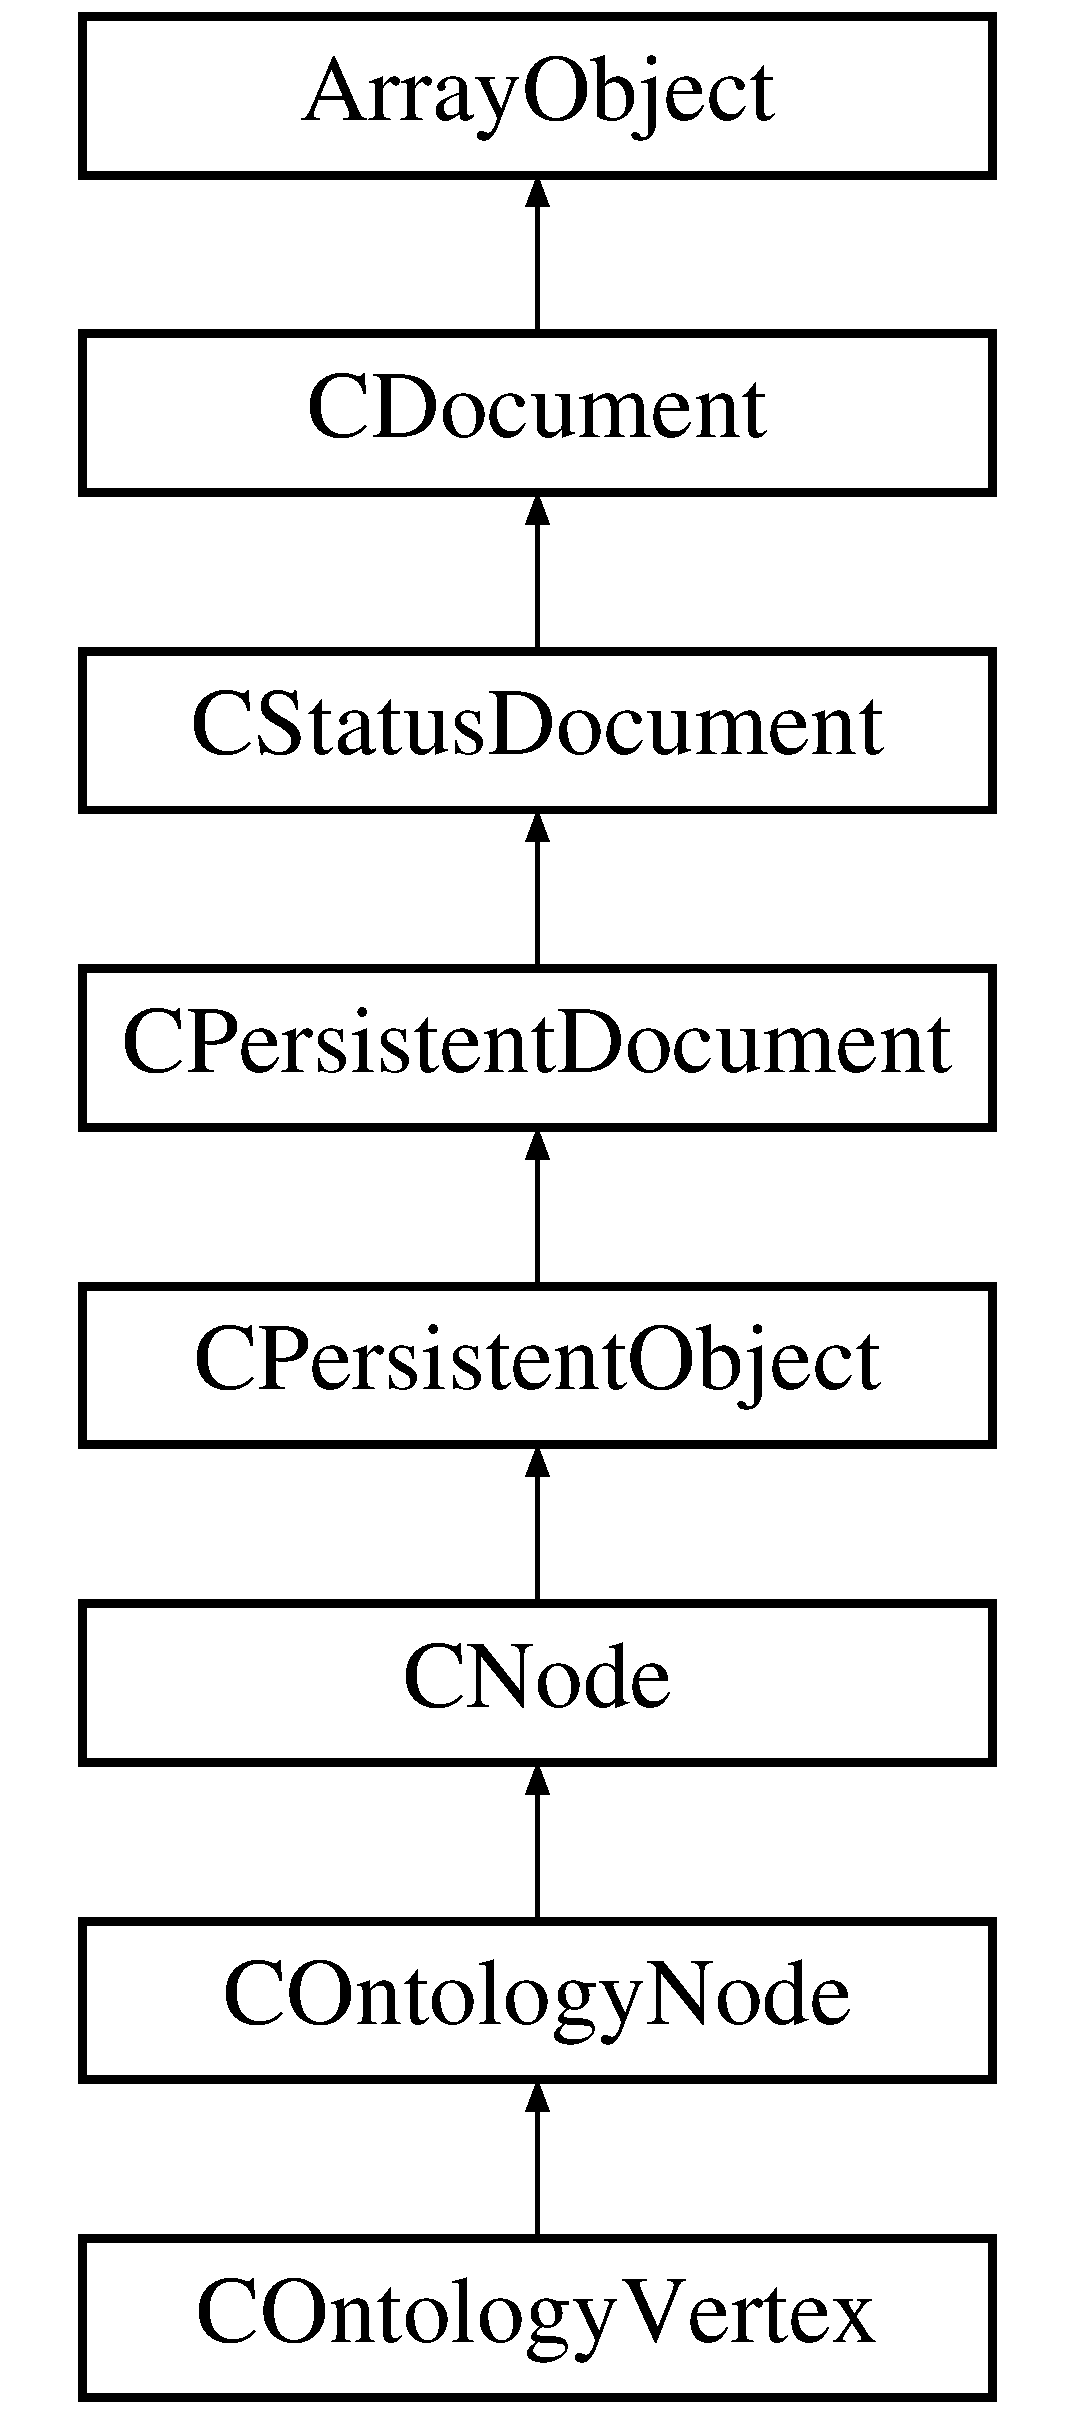
\includegraphics[height=8.000000cm]{class_c_ontology_vertex}
\end{center}
\end{figure}
\subsection*{Protected Member Functions}
\begin{DoxyCompactItemize}
\item 
\hyperlink{class_c_ontology_vertex_aa2380ad2c704a212492549f56b9ed18f}{\-\_\-\-Term\-Attributes} ()
\end{DoxyCompactItemize}
\subsection*{Additional Inherited Members}


\subsection{Member Function Documentation}
\hypertarget{class_c_ontology_vertex_aa2380ad2c704a212492549f56b9ed18f}{\index{C\-Ontology\-Vertex@{C\-Ontology\-Vertex}!\-\_\-\-Term\-Attributes@{\-\_\-\-Term\-Attributes}}
\index{\-\_\-\-Term\-Attributes@{\-\_\-\-Term\-Attributes}!COntologyVertex@{C\-Ontology\-Vertex}}
\subsubsection[{\-\_\-\-Term\-Attributes}]{\setlength{\rightskip}{0pt plus 5cm}C\-Ontology\-Vertex\-::\-\_\-\-Term\-Attributes (
\begin{DoxyParamCaption}
{}
\end{DoxyParamCaption}
)\hspace{0.3cm}{\ttfamily [protected]}}}\label{class_c_ontology_vertex_aa2380ad2c704a212492549f56b9ed18f}
\subparagraph*{List term attributes}

In this class we return\-:


\begin{DoxyItemize}
\item {\ttfamily \hyperlink{}{k\-T\-A\-G\-\_\-\-L\-I\-D}}\-: The local identifier. 
\item {\ttfamily \hyperlink{}{k\-T\-A\-G\-\_\-\-G\-I\-D}}\-: The global identifier. 
\item {\ttfamily \hyperlink{}{k\-T\-A\-G\-\_\-\-L\-A\-B\-E\-L}}\-: The label. 
\item {\ttfamily \hyperlink{}{k\-T\-A\-G\-\_\-\-D\-E\-F\-I\-N\-I\-T\-I\-O\-N}}\-: The definition. 
\item {\ttfamily \hyperlink{}{k\-T\-A\-G\-\_\-\-F\-E\-A\-T\-U\-R\-E\-S}}\-: The feature tag references. 
\item {\ttfamily \hyperlink{}{k\-T\-A\-G\-\_\-\-S\-C\-A\-L\-E\-S}}\-: The scale tag references. 
\end{DoxyItemize}

protected \begin{DoxyReturn}{Returns}
array 
\end{DoxyReturn}


The documentation for this class was generated from the following file\-:\begin{DoxyCompactItemize}
\item 
/\-Library/\-Web\-Server/\-Library/\-P\-H\-P\-Wrapper/classes/C\-Ontology\-Vertex.\-php\end{DoxyCompactItemize}

\hypertarget{class_c_ontology_wrapper}{\section{C\-Ontology\-Wrapper Class Reference}
\label{class_c_ontology_wrapper}\index{C\-Ontology\-Wrapper@{C\-Ontology\-Wrapper}}
}
Inheritance diagram for C\-Ontology\-Wrapper\-:\begin{figure}[H]
\begin{center}
\leavevmode
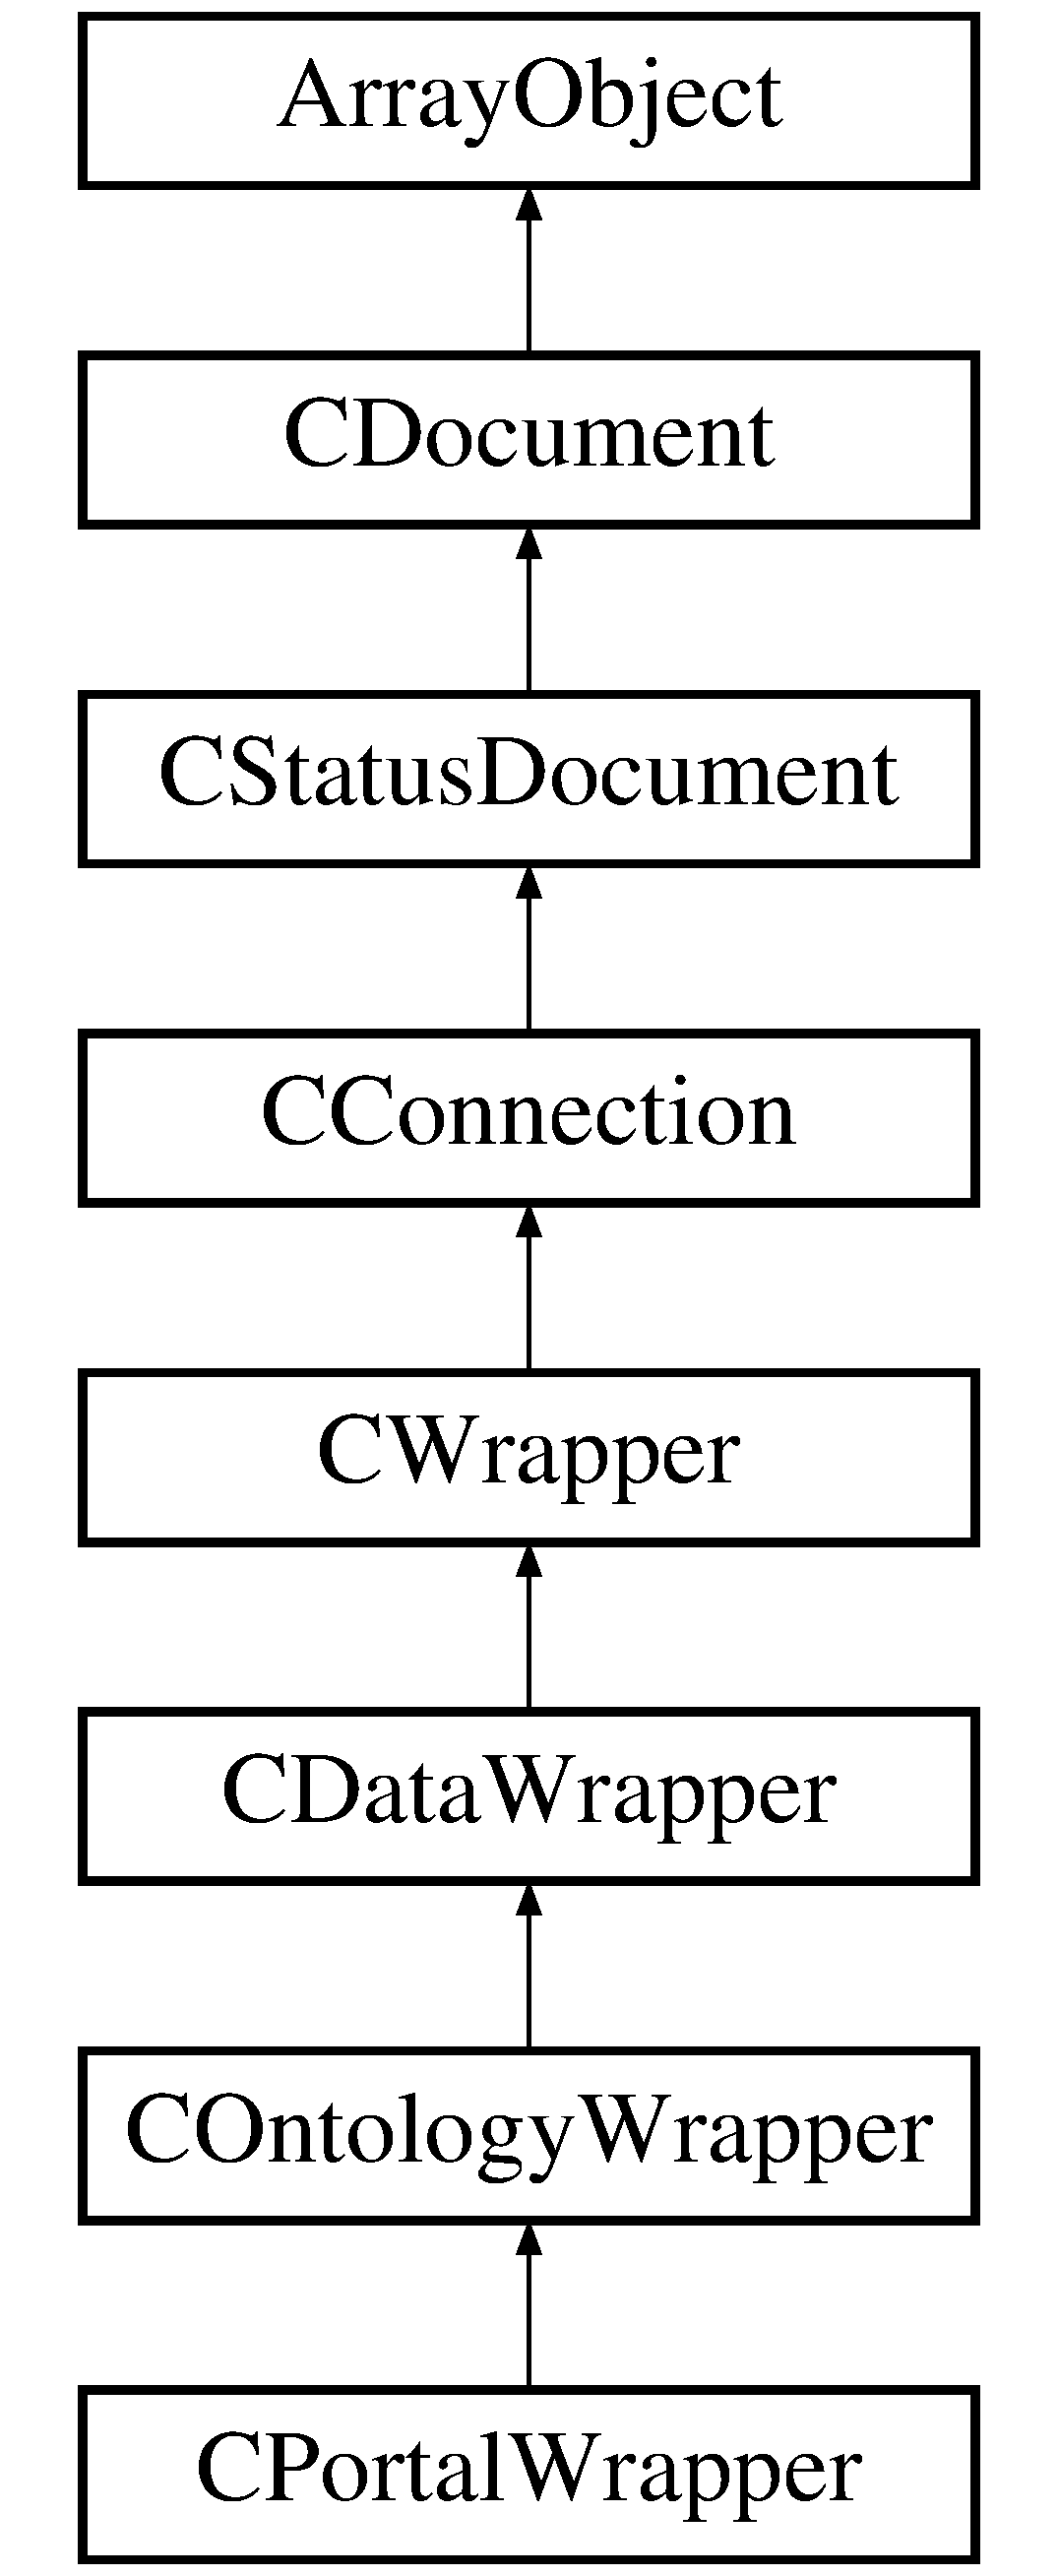
\includegraphics[height=8.000000cm]{class_c_ontology_wrapper}
\end{center}
\end{figure}
\subsection*{Public Member Functions}
\begin{DoxyCompactItemize}
\item 
\hyperlink{class_c_ontology_wrapper_a7d37edd771ffa60b36ead632c2e46534}{\-\_\-\-Build\-Term} (\$the\-Term)
\item 
\hyperlink{class_c_ontology_wrapper_a3149d34bb488513db2d572f3002bebce}{\-\_\-\-Build\-Node} (\$the\-Node)
\end{DoxyCompactItemize}
\subsection*{Static Public Attributes}
\begin{DoxyCompactItemize}
\item 
static {\bfseries \$s\-Parameter\-List}
\end{DoxyCompactItemize}
\subsection*{Protected Member Functions}
\begin{DoxyCompactItemize}
\item 
\hyperlink{class_c_ontology_wrapper_a744158c5f34f6b609332386e7fa3dcc0}{\-\_\-\-Parse\-Request} ()
\item 
\hyperlink{class_c_ontology_wrapper_a3c8d6b45c1a7439863c7a7c624685fe6}{\-\_\-\-Format\-Request} ()
\item 
\hyperlink{class_c_ontology_wrapper_a1804be7ffd6f2c76911757e248721ed0}{\-\_\-\-Validate\-Request} ()
\item 
\hyperlink{class_c_ontology_wrapper_a6a0b9b8f007455703af1f13901d07e6a}{\-\_\-\-Init\-Parameters} ()
\item 
\hyperlink{class_c_ontology_wrapper_aafcb67362b104e456f5021f5ac8d953c}{\-\_\-\-Parse\-Operation} ()
\item 
\hyperlink{class_c_ontology_wrapper_acd547aac2e68a0af8087205ac3936f96}{\-\_\-\-Parse\-Language} ()
\item 
\hyperlink{class_c_ontology_wrapper_ac7d6e87ccce8614f023b517944afe2e1}{\-\_\-\-Parse\-Predicate} ()
\item 
\hyperlink{class_c_ontology_wrapper_a7a42ec2eec0c2a3e541ee9f01c8ffc1d}{\-\_\-\-Parse\-Relation} ()
\item 
\hyperlink{class_c_ontology_wrapper_af15ee180d487325af0bb45a21fd559e8}{\-\_\-\-Parse\-Subquery} ()
\item 
\hyperlink{class_c_ontology_wrapper_adb70ad81542bd5fa3a9d3e99bb1226ae}{\-\_\-\-Parse\-Rel\-Subject} ()
\item 
\hyperlink{class_c_ontology_wrapper_a2318ee98558d1821d04617a51761ff57}{\-\_\-\-Parse\-Rel\-Object} ()
\item 
\hyperlink{class_c_ontology_wrapper_ac44f7108d423e9b9a846a8505f0ea4ad}{\-\_\-\-Parse\-Rel\-Mirror} ()
\item 
\hyperlink{class_c_ontology_wrapper_a9eb4cc1d7cad579780d9992d1b63e722}{\-\_\-\-Format\-Language} ()
\item 
\hyperlink{class_c_ontology_wrapper_a3dbe14a223ba9573de23a39cdffc78ce}{\-\_\-\-Format\-Predicate} ()
\item 
\hyperlink{class_c_ontology_wrapper_a075931ffaafe656e8829c14f6f8c53e8}{\-\_\-\-Format\-Relation} ()
\item 
\hyperlink{class_c_ontology_wrapper_a9391d5006fda356996db159f4e7ae729}{\-\_\-\-Format\-Subquery} ()
\item 
\hyperlink{class_c_ontology_wrapper_a6c5f76307abce4bbec7873b872452cc4}{\-\_\-\-Format\-Rel\-Subject} ()
\item 
\hyperlink{class_c_ontology_wrapper_a96ba7e0a267060ac2e1e13f885361125}{\-\_\-\-Format\-Rel\-Object} ()
\item 
\hyperlink{class_c_ontology_wrapper_ac2b2dbf74b54dba53bbf37bc3a0a3370}{\-\_\-\-Format\-Rel\-Mirror} ()
\item 
\hyperlink{class_c_ontology_wrapper_ab3c0f2985e63ebde5294f69e7d501ecb}{\-\_\-\-Validate\-Operation} ()
\item 
\hyperlink{class_c_ontology_wrapper_ae7f6ac49de190887d0d909edaba49862}{\-\_\-\-Validate\-Query} ()
\item 
\hyperlink{class_c_ontology_wrapper_a0a84083f3ba78aabf06d72d75bb3857c}{\-\_\-\-Validate\-Object} ()
\item 
\hyperlink{class_c_ontology_wrapper_aa3fb91ea57bbf16ceab2c80fc2aa52f8}{\-\_\-\-Validate\-Language} ()
\item 
\hyperlink{class_c_ontology_wrapper_a6dd38a830784c98b6da00f935e90b119}{\-\_\-\-Validate\-Predicate} ()
\item 
\hyperlink{class_c_ontology_wrapper_a9f720d10bd6ebe66801b3b1c2f96bf1d}{\-\_\-\-Validate\-Relation} ()
\item 
\hyperlink{class_c_ontology_wrapper_ae3b189d33f445d6182c2626cf914347d}{\-\_\-\-Validate\-Subquery} ()
\item 
\hyperlink{class_c_ontology_wrapper_a5102d350704cef1af5fb426c07bfaed6}{\-\_\-\-Validate\-Rel\-Subject} ()
\item 
\hyperlink{class_c_ontology_wrapper_a427fc121127a26c1c5ee114678f3f799}{\-\_\-\-Validate\-Rel\-Object} ()
\item 
\hyperlink{class_c_ontology_wrapper_ab748adddd32f9a703ea58921c1717613}{\-\_\-\-Validate\-Rel\-Mirror} ()
\item 
\hyperlink{class_c_ontology_wrapper_ad3cd51256856ae11799d51b8be692b75}{\-\_\-\-Handle\-Request} ()
\item 
\hyperlink{class_c_ontology_wrapper_a74d55eb1d9cc06402c788a0106622b12}{\-\_\-\-Handle\-\_\-\-List\-Op} (\&\$the\-List)
\item 
\hyperlink{class_c_ontology_wrapper_af17889957c64e8e97e2f013a5117a547}{\-\_\-\-Handle\-\_\-\-Set\-Term} ()
\item 
\hyperlink{class_c_ontology_wrapper_a64c0266dc4b914cf73863aa59caf0746}{\-\_\-\-Handle\-\_\-\-Get\-Term} ()
\item 
\hyperlink{class_c_ontology_wrapper_a0634a48b2fa3ffc6b9b229c7e63d1611}{\-\_\-\-Handle\-\_\-\-Set\-Vertex} ()
\item 
\hyperlink{class_c_ontology_wrapper_a9a2e6b3a9911dcfe1b1e5bffc20f451e}{\-\_\-\-Handle\-\_\-\-Get\-Vertex} ()
\item 
\hyperlink{class_c_ontology_wrapper_aa25444a57bb5746f743a2195667ea4de}{\-\_\-\-Handle\-Get\-Tag} ()
\item 
\hyperlink{class_c_ontology_wrapper_a38e3d92a704e327580c541e0bf0c51b0}{\-\_\-\-Handle\-Relate\-To} ()
\item 
\hyperlink{class_c_ontology_wrapper_a97cffdfee4bb6d7841201dd2bc7fd0f2}{\-\_\-\-Handle\-Get\-Enums} ()
\item 
\hyperlink{class_c_ontology_wrapper_a4e4ca830c618987caaa7dd0542e73dcf}{\-\_\-\-Export\-Term} (\&\$the\-Collection, \$the\-Term, \$do\-Tags=T\-R\-U\-E)
\item 
\hyperlink{class_c_ontology_wrapper_aeeb219d5ec2e33ec4fb1deb8f8c2284e}{\-\_\-\-Export\-Node} (\&\$the\-Collection, \$the\-Node, \$do\-Tags=T\-R\-U\-E)
\item 
\hyperlink{class_c_ontology_wrapper_a116afbf3c771558c63857a3be172d3a5}{\-\_\-\-Export\-Edge} (\&\$the\-Collection, \$the\-Edge, \$do\-Tags=T\-R\-U\-E)
\item 
\hyperlink{class_c_ontology_wrapper_a7f295f7da04d526b963fac0d2ddbc362}{\-\_\-\-Export\-Tag} (\&\$the\-Collection, \$the\-Tag)
\item 
\hyperlink{class_c_ontology_wrapper_aabedfd89f1829927c2f115073e2805f4}{\-\_\-\-Get\-Vertex\-List} ()
\item 
\hyperlink{class_c_ontology_wrapper_a6743af8581329c1fb5ccd2dc860b0701}{\-\_\-\-Get\-Related\-Query} (\$the\-Vertex)
\item 
\hyperlink{class_c_ontology_wrapper_a851254326f30e2be713ff8138e4ded07}{\-\_\-\-Get\-Related\-Subquery} (\hyperlink{class_c_query}{C\-Query} \$the\-Query, \$the\-Vertex)
\item 
\hyperlink{class_c_ontology_wrapper_ae479b8f21490acc903bdc9a27875de9e}{\-\_\-\-Filter\-Languages} (\$the\-Languages)
\item 
\hyperlink{class_c_ontology_wrapper_a44b44339e82da36fdffe6d76f71aa2e8}{\-\_\-\-Resolve\-Enumerations} (\hyperlink{class_c_container}{C\-Container} \$the\-Container)
\item 
\hyperlink{class_c_ontology_wrapper_a825424d5394114f69acb8edcc45b05a5}{\-\_\-\-Normalise\-Term\-References} (\&\$the\-Query)
\end{DoxyCompactItemize}
\subsection*{Additional Inherited Members}


\subsection{Member Function Documentation}
\hypertarget{class_c_ontology_wrapper_a3149d34bb488513db2d572f3002bebce}{\index{C\-Ontology\-Wrapper@{C\-Ontology\-Wrapper}!\-\_\-\-Build\-Node@{\-\_\-\-Build\-Node}}
\index{\-\_\-\-Build\-Node@{\-\_\-\-Build\-Node}!COntologyWrapper@{C\-Ontology\-Wrapper}}
\subsubsection[{\-\_\-\-Build\-Node}]{\setlength{\rightskip}{0pt plus 5cm}C\-Ontology\-Wrapper\-::\-\_\-\-Build\-Node (
\begin{DoxyParamCaption}
\item[{}]{\$the\-Node}
\end{DoxyParamCaption}
)}}\label{class_c_ontology_wrapper_a3149d34bb488513db2d572f3002bebce}
\subparagraph*{Build a vertex}

The main duty of this method is to resolve the provided node's references and return a single object that merges all its term and node attributes.

Since we use a document database to store the graph vertices index, it is better to store referenced data in the vertex object, so that it is easier to search.

In this class we therefore return the object as-\/is, in derived classes we can use this method for other purposes.


\begin{DoxyParams}[1]{Parameters}
mixed & {\em \$the\-Node} & Node object.\\
\hline
\end{DoxyParams}
public \begin{DoxyReturn}{Returns}
array Vertex object. 
\end{DoxyReturn}
\hypertarget{class_c_ontology_wrapper_a7d37edd771ffa60b36ead632c2e46534}{\index{C\-Ontology\-Wrapper@{C\-Ontology\-Wrapper}!\-\_\-\-Build\-Term@{\-\_\-\-Build\-Term}}
\index{\-\_\-\-Build\-Term@{\-\_\-\-Build\-Term}!COntologyWrapper@{C\-Ontology\-Wrapper}}
\subsubsection[{\-\_\-\-Build\-Term}]{\setlength{\rightskip}{0pt plus 5cm}C\-Ontology\-Wrapper\-::\-\_\-\-Build\-Term (
\begin{DoxyParamCaption}
\item[{}]{\$the\-Term}
\end{DoxyParamCaption}
)}}\label{class_c_ontology_wrapper_a7d37edd771ffa60b36ead632c2e46534}
\subparagraph*{Build a term}

The main duty of this method is to resolve the provided term reference and return a single object that holds a merged selection of attributes.

By default we include the \hyperlink{}{k\-T\-A\-G\-\_\-\-L\-I\-D}, \hyperlink{}{k\-T\-A\-G\-\_\-\-G\-I\-D} and the \hyperlink{}{k\-T\-A\-G\-\_\-\-N\-A\-M\-E\-S\-P\-A\-C\-E} (resolved into the referenced \hyperlink{}{k\-T\-A\-G\-\_\-\-G\-I\-D}) from the current term.

We omit the \hyperlink{}{k\-T\-A\-G\-\_\-\-N\-I\-D}, \hyperlink{}{k\-T\-A\-G\-\_\-\-C\-L\-A\-S\-S}, \hyperlink{}{k\-T\-E\-R\-M\-\_\-\-T\-E\-R\-M}, \hyperlink{}{k\-T\-E\-R\-M\-\_\-\-N\-A\-M\-E\-S\-P\-A\-C\-E\-\_\-\-R\-E\-F\-S} and \hyperlink{}{k\-T\-E\-R\-M\-\_\-\-N\-O\-D\-E\-S}.

All other attributes will either be included from the current term, or, if the term is related to another term through its \hyperlink{}{k\-T\-E\-R\-M\-\_\-\-T\-E\-R\-M} attribute, from that term.

The method will raise an exception if any element cannot be resolved.


\begin{DoxyParams}[1]{Parameters}
mixed & {\em \$the\-Term} & Term reference or object.\\
\hline
\end{DoxyParams}
public \begin{DoxyReturn}{Returns}
array Exported term. 
\end{DoxyReturn}
\hypertarget{class_c_ontology_wrapper_a116afbf3c771558c63857a3be172d3a5}{\index{C\-Ontology\-Wrapper@{C\-Ontology\-Wrapper}!\-\_\-\-Export\-Edge@{\-\_\-\-Export\-Edge}}
\index{\-\_\-\-Export\-Edge@{\-\_\-\-Export\-Edge}!COntologyWrapper@{C\-Ontology\-Wrapper}}
\subsubsection[{\-\_\-\-Export\-Edge}]{\setlength{\rightskip}{0pt plus 5cm}C\-Ontology\-Wrapper\-::\-\_\-\-Export\-Edge (
\begin{DoxyParamCaption}
\item[{\&}]{\$the\-Collection, }
\item[{}]{\$the\-Edge, }
\item[{}]{\$do\-Tags = {\ttfamily TRUE}}
\end{DoxyParamCaption}
)\hspace{0.3cm}{\ttfamily [protected]}}}\label{class_c_ontology_wrapper_a116afbf3c771558c63857a3be172d3a5}
\subparagraph*{Export an edge}

The main duty of this method is to normalise the edge's attributes and store the referenced vertex and predicates in the relative elements of the provided collection.

The method expects the following parameters\-:


\begin{DoxyItemize}
\item {\ttfamily \&\$the\-Collection}\-: This parameter is a reference to an array that will receive the object attributes, the array holds four lists that collect similar objects, such as nodes, terms, edges and tags\-: 
\begin{DoxyItemize}
\item {\ttfamily \hyperlink{}{k\-A\-P\-I\-\_\-\-C\-O\-L\-L\-E\-C\-T\-I\-O\-N\-\_\-\-I\-D}}\-: This element is an array that holds the identifiers list of the requested elements. This element should be filled by the caller, since its content depend on what operation is going on. 
\item {\ttfamily \hyperlink{}{k\-A\-P\-I\-\_\-\-C\-O\-L\-L\-E\-C\-T\-I\-O\-N\-\_\-\-T\-E\-R\-M}}\-: This element is an array that holds the list of predicate terms referenced by all other objects in the collection. The array keys will be the term's \hyperlink{}{k\-T\-A\-G\-\_\-\-G\-I\-D} and the value will be the attributes of the term. The contents of this element are fed with the \hyperlink{class_c_ontology_wrapper_a7d37edd771ffa60b36ead632c2e46534}{\-\_\-\-Build\-Term()} protected method to which the edge predicates will be provided. 
\item {\ttfamily \hyperlink{}{k\-A\-P\-I\-\_\-\-C\-O\-L\-L\-E\-C\-T\-I\-O\-N\-\_\-\-N\-O\-D\-E}}\-: This element is an array that holds a list of node vertex. A vertex is the combination of the node attributes merged with the referenced term attributes. The items of this list are indexed by the node \hyperlink{}{k\-T\-A\-G\-\_\-\-N\-I\-D} and eventual term attributes are overwritten by matching node attributes. The contents of this element are fed by the \hyperlink{class_c_ontology_wrapper_a3149d34bb488513db2d572f3002bebce}{\-\_\-\-Build\-Node()} protected method to which both the object and subject vertices will be provided. 
\item {\ttfamily \hyperlink{}{k\-A\-P\-I\-\_\-\-C\-O\-L\-L\-E\-C\-T\-I\-O\-N\-\_\-\-E\-D\-G\-E}}\-: This element is an array that holds a list of edges, the array keys will be the edge's \hyperlink{}{k\-T\-A\-G\-\_\-\-G\-I\-D} and the value will be the edge's attributes. The contents of this element are fed by the \hyperlink{}{\-\_\-\-Build\-Edge()} protected method. 
\item {\ttfamily \hyperlink{}{k\-A\-P\-I\-\_\-\-C\-O\-L\-L\-E\-C\-T\-I\-O\-N\-\_\-\-T\-A\-G}}\-: This element is an array that holds a list of tags, the array indexes will be the tag \hyperlink{}{k\-T\-A\-G\-\_\-\-N\-I\-D} and the array values will be the tag \hyperlink{}{k\-T\-A\-G\-\_\-\-P\-A\-T\-H} and \hyperlink{}{k\-T\-A\-G\-\_\-\-G\-I\-D}, where the \hyperlink{}{k\-T\-A\-G\-\_\-\-P\-A\-T\-H} predicate references will be set to the term \hyperlink{}{k\-T\-A\-G\-\_\-\-G\-I\-D}. 
\end{DoxyItemize}
\item {\ttfamily \$the\-Edge}\-: This parameter represents the edge object or a list of edges\-: 
\begin{DoxyItemize}
\item {\ttfamily array}\-: A list of edges. 
\item {\ttfamily \hyperlink{class_c_ontology_edge}{C\-Ontology\-Edge}}\-: The edge will be used as-\/is. 
\end{DoxyItemize}
\end{DoxyItemize}

The method will omit the \hyperlink{}{k\-T\-A\-G\-\_\-\-U\-I\-D} and \hyperlink{}{k\-T\-A\-G\-\_\-\-C\-L\-A\-S\-S} attributes, the \hyperlink{}{k\-T\-A\-G\-\_\-\-P\-R\-E\-D\-I\-C\-A\-T\-E} attribute will be set to the term's \hyperlink{}{k\-T\-A\-G\-\_\-\-G\-I\-D} attribute and the two vertex references will be left untouched. The resulting array will be set into the \hyperlink{}{k\-O\-F\-F\-S\-E\-T\-\_\-\-E\-X\-P\-O\-R\-T\-\_\-\-E\-D\-G\-E} element of the provided collection.

The method will raise an exception if any element cannot be resolved.


\begin{DoxyParams}[1]{Parameters}
reference & {\em \&\$the\-Collection} & Exported collection. \\
\hline
mixed & {\em \$the\-Edge} & Edge or edges list. \\
\hline
boolean & {\em \$do\-Tags} & T\-R\-U\-E means load tags.\\
\hline
\end{DoxyParams}
protected


\begin{DoxyExceptions}{Exceptions}
{\em Exception} & \\
\hline
\end{DoxyExceptions}
\hypertarget{class_c_ontology_wrapper_aeeb219d5ec2e33ec4fb1deb8f8c2284e}{\index{C\-Ontology\-Wrapper@{C\-Ontology\-Wrapper}!\-\_\-\-Export\-Node@{\-\_\-\-Export\-Node}}
\index{\-\_\-\-Export\-Node@{\-\_\-\-Export\-Node}!COntologyWrapper@{C\-Ontology\-Wrapper}}
\subsubsection[{\-\_\-\-Export\-Node}]{\setlength{\rightskip}{0pt plus 5cm}C\-Ontology\-Wrapper\-::\-\_\-\-Export\-Node (
\begin{DoxyParamCaption}
\item[{\&}]{\$the\-Collection, }
\item[{}]{\$the\-Node, }
\item[{}]{\$do\-Tags = {\ttfamily TRUE}}
\end{DoxyParamCaption}
)\hspace{0.3cm}{\ttfamily [protected]}}}\label{class_c_ontology_wrapper_aeeb219d5ec2e33ec4fb1deb8f8c2284e}
\subparagraph*{Export a vertex}

The main duty of this method is to export a collection of vertex nodes into a series of collections each holding a class of data. The method will have to resolve eventual references and store the resolved data in their corresponding collection.

The method expects the following parameters\-:


\begin{DoxyItemize}
\item {\ttfamily \&\$the\-Collection}\-: This parameter is a reference to an array that will receive the object attributes, the array holds four lists that collect objects of the same class\-: 
\begin{DoxyItemize}
\item {\ttfamily \hyperlink{}{k\-A\-P\-I\-\_\-\-C\-O\-L\-L\-E\-C\-T\-I\-O\-N\-\_\-\-I\-D}}\-: This element is an array that holds the identifiers list of the requested elements. Depending on what was requested, this list will hold term, node, edge or tag identifiers. 
\item {\ttfamily \hyperlink{}{k\-A\-P\-I\-\_\-\-C\-O\-L\-L\-E\-C\-T\-I\-O\-N\-\_\-\-T\-E\-R\-M}}\-: This element is an array that holds the list of terms referenced by all other objects in the collection. The array keys will be the term's \hyperlink{}{k\-T\-A\-G\-\_\-\-G\-I\-D} and the value the term attributes. The contents of this element are fed by the \hyperlink{class_c_ontology_wrapper_a7d37edd771ffa60b36ead632c2e46534}{\-\_\-\-Build\-Term()} protected method. 
\item {\ttfamily \hyperlink{}{k\-A\-P\-I\-\_\-\-C\-O\-L\-L\-E\-C\-T\-I\-O\-N\-\_\-\-N\-O\-D\-E}}\-: This element is an array that holds a list of node vertex. A vertex is the combination of the node attributes merged with the referenced term attributes. The items of this list are indexed by the node \hyperlink{}{k\-T\-A\-G\-\_\-\-N\-I\-D} and eventual term attributes are overwritten by matching node attributes. The contents of this element are fed by the \hyperlink{class_c_ontology_wrapper_a3149d34bb488513db2d572f3002bebce}{\-\_\-\-Build\-Node()} protected method. 
\item {\ttfamily \hyperlink{}{k\-A\-P\-I\-\_\-\-C\-O\-L\-L\-E\-C\-T\-I\-O\-N\-\_\-\-E\-D\-G\-E}}\-: This element is an array that holds a list of edges, the array keys will be the edge's \hyperlink{}{k\-T\-A\-G\-\_\-\-G\-I\-D} and the value will be the edge's attributes. The contents of this element are fed by the \hyperlink{}{\-\_\-\-Build\-Edge()} protected method. 
\item {\ttfamily \hyperlink{}{k\-A\-P\-I\-\_\-\-C\-O\-L\-L\-E\-C\-T\-I\-O\-N\-\_\-\-T\-A\-G}}\-: This element is an array that holds a list of tags, the array indexes will be the tag \hyperlink{}{k\-T\-A\-G\-\_\-\-N\-I\-D} and the array values will be the tag \hyperlink{}{k\-T\-A\-G\-\_\-\-P\-A\-T\-H} and \hyperlink{}{k\-T\-A\-G\-\_\-\-G\-I\-D}, where the \hyperlink{}{k\-T\-A\-G\-\_\-\-P\-A\-T\-H} predicate references will be set to the term \hyperlink{}{k\-T\-A\-G\-\_\-\-G\-I\-D}. 
\end{DoxyItemize}
\item {\ttfamily \$the\-Node}\-: This parameter represents the vertex node full object; this means that all attributes should be present, since this method will take care of removing unwanted attributes. The parameter may represent a list of node objects or references, a reference or an object\-: 
\begin{DoxyItemize}
\item {\ttfamily array}\-: Each element of the list will be fed to this method recursively. 
\item {\ttfamily \hyperlink{class_c_ontology_node}{C\-Ontology\-Node}}\-: The object will be used as is. 
\item {\itshape other}\-: Any other type will be interpreted as a node reference. 
\end{DoxyItemize}
\item {\ttfamily \$the\-Attributes}\-: This optional parameter can be used to limit the returned attributes to the list provided in this array. 
\item {\ttfamily \$do\-Tags}\-: If this flag is {\ttfamily T\-R\-U\-E}, the method will load the tags; if {\ttfamily F\-A\-L\-S\-E} no tags will be loaded. 
\end{DoxyItemize}

The method will generate an array containing the merged attributes of the node and the referenced term, this array will be set in the \hyperlink{}{k\-A\-P\-I\-\_\-\-C\-O\-L\-L\-E\-C\-T\-I\-O\-N\-\_\-\-N\-O\-D\-E} of the {\ttfamily \&\$the\-Collection} parameter with as index the node \hyperlink{}{k\-T\-A\-G\-\_\-\-N\-I\-D} that will ve added to the \hyperlink{}{k\-A\-P\-I\-\_\-\-C\-O\-L\-L\-E\-C\-T\-I\-O\-N\-\_\-\-I\-D} element of the collection.

If a matching vertex already exists in the {\ttfamily \&\$the\-Collection} parameter, the method will do nothing.

For more information please consult the \hyperlink{class_c_ontology_wrapper_a3149d34bb488513db2d572f3002bebce}{\-\_\-\-Build\-Node()} method reference, note that this method will remove the \hyperlink{}{k\-T\-A\-G\-\_\-\-N\-I\-D} attribute from the node, it will only use this information to index the node.

The method will raise an exception if any element cannot be resolved.


\begin{DoxyParams}[1]{Parameters}
reference & {\em \&\$the\-Collection} & Exported collection. \\
\hline
mixed & {\em \$the\-Node} & Node identifier or list. \\
\hline
boolean & {\em \$do\-Tags} & T\-R\-U\-E means load tags.\\
\hline
\end{DoxyParams}
protected \hypertarget{class_c_ontology_wrapper_a7f295f7da04d526b963fac0d2ddbc362}{\index{C\-Ontology\-Wrapper@{C\-Ontology\-Wrapper}!\-\_\-\-Export\-Tag@{\-\_\-\-Export\-Tag}}
\index{\-\_\-\-Export\-Tag@{\-\_\-\-Export\-Tag}!COntologyWrapper@{C\-Ontology\-Wrapper}}
\subsubsection[{\-\_\-\-Export\-Tag}]{\setlength{\rightskip}{0pt plus 5cm}C\-Ontology\-Wrapper\-::\-\_\-\-Export\-Tag (
\begin{DoxyParamCaption}
\item[{\&}]{\$the\-Collection, }
\item[{}]{\$the\-Tag}
\end{DoxyParamCaption}
)\hspace{0.3cm}{\ttfamily [protected]}}}\label{class_c_ontology_wrapper_a7f295f7da04d526b963fac0d2ddbc362}
\subparagraph*{Export a tag}

The main duty of this method is to normalise the tag's attributes and store the referenced predicates and vertices in the relative elements of the provided collection.

The method expects the following parameters\-:


\begin{DoxyItemize}
\item {\ttfamily \&\$the\-Collection}\-: This parameter is a reference to an array that will receive the object attributes, the array holds four lists that collect similar objects, such as nodes, terms, edges and tags\-: 
\begin{DoxyItemize}
\item {\ttfamily \hyperlink{}{k\-A\-P\-I\-\_\-\-C\-O\-L\-L\-E\-C\-T\-I\-O\-N\-\_\-\-I\-D}}\-: This element is an array that holds the identifiers list of the requested elements. This element is ignored by this method. 
\item {\ttfamily \hyperlink{}{k\-A\-P\-I\-\_\-\-C\-O\-L\-L\-E\-C\-T\-I\-O\-N\-\_\-\-T\-E\-R\-M}}\-: This element is an array that holds the list of predicate terms referenced by all other objects in the collection. The array keys will be the term's \hyperlink{}{k\-T\-A\-G\-\_\-\-G\-I\-D} and the value will be the attributes of the term. The contents of this element are fed by the \hyperlink{class_c_ontology_wrapper_a7d37edd771ffa60b36ead632c2e46534}{\-\_\-\-Build\-Term()} protected method. 
\item {\ttfamily \hyperlink{}{k\-A\-P\-I\-\_\-\-C\-O\-L\-L\-E\-C\-T\-I\-O\-N\-\_\-\-N\-O\-D\-E}}\-: This element is an array that holds a list of node vertex. A vertex is the combination of the node attributes merged with the referenced term attributes. The items of this list are indexed by the node \hyperlink{}{k\-T\-A\-G\-\_\-\-N\-I\-D} and eventual term attributes are overwritten by matching node attributes. The contents of this element are fed by the \hyperlink{class_c_ontology_wrapper_a3149d34bb488513db2d572f3002bebce}{\-\_\-\-Build\-Node()} protected method. 
\item {\ttfamily \hyperlink{}{k\-A\-P\-I\-\_\-\-C\-O\-L\-L\-E\-C\-T\-I\-O\-N\-\_\-\-E\-D\-G\-E}}\-: This element is an array that holds a list of edges, the array keys will be the edge's \hyperlink{}{k\-T\-A\-G\-\_\-\-G\-I\-D} and the value will be the edge's attributes. The contents of this element are fed by the \hyperlink{}{\-\_\-\-Build\-Edge()} protected method. 
\item {\ttfamily \hyperlink{}{k\-A\-P\-I\-\_\-\-C\-O\-L\-L\-E\-C\-T\-I\-O\-N\-\_\-\-T\-A\-G}}\-: This element is an array that holds a list of tags, the array indexes will be the tag \hyperlink{}{k\-T\-A\-G\-\_\-\-N\-I\-D} and the array values will be the tag \hyperlink{}{k\-T\-A\-G\-\_\-\-P\-A\-T\-H} and \hyperlink{}{k\-T\-A\-G\-\_\-\-G\-I\-D}, where the \hyperlink{}{k\-T\-A\-G\-\_\-\-P\-A\-T\-H} predicate references will be set to the term \hyperlink{}{k\-T\-A\-G\-\_\-\-G\-I\-D}. This method will fill this element. 
\end{DoxyItemize}
\item {\ttfamily \$the\-Tag}\-: This parameter represents the tag identifier, object or a list of tag identifiers\-: 
\begin{DoxyItemize}
\item {\ttfamily array}\-: A list of tag or node identifiers. 
\item {\ttfamily \hyperlink{class_c_ontology_tag}{C\-Ontology\-Tag}}\-: The tag will be used as-\/is. 
\item {\itshape other}\-: Any other type will be interpreted as a tag reference and resolved with \hyperlink{}{Resolve\-Tag()}. 
\end{DoxyItemize}
\item {\ttfamily \$the\-Attributes}\-: This optional parameter can be used to limit the returned attributes to the list provided in this array. 
\end{DoxyItemize}

The method will generate an array containing the merged attributes of the tag and the exported attributes of the referenced nodes, generated by the \hyperlink{class_c_ontology_wrapper_aeeb219d5ec2e33ec4fb1deb8f8c2284e}{\-\_\-\-Export\-Node()} protected method. The method will exclude the \hyperlink{}{k\-T\-A\-G\-\_\-\-N\-I\-D}, \hyperlink{}{k\-T\-A\-G\-\_\-\-U\-I\-D}, and \hyperlink{}{k\-T\-A\-G\-\_\-\-C\-L\-A\-S\-S} from the tag, but append all others to the merged node and term attributes. The predicate elements of the \hyperlink{}{K\-T\-A\-G\-\_\-\-P\-A\-T\-H} attribute will be set to the referenced term's \hyperlink{}{k\-T\-A\-G\-\_\-\-G\-I\-D}. The resulting array will be set in the \hyperlink{}{k\-O\-F\-F\-S\-E\-T\-\_\-\-E\-X\-P\-O\-R\-T\-\_\-\-T\-A\-G} element of the provided collection using the tag's \hyperlink{}{k\-T\-A\-G\-\_\-\-N\-I\-D} attribute as index.

The method will raise an exception if any element cannot be resolved.


\begin{DoxyParams}[1]{Parameters}
reference & {\em \&\$the\-Collection} & Exported collection. \\
\hline
mixed & {\em \$the\-Tag} & Tag identifier or list.\\
\hline
\end{DoxyParams}
protected


\begin{DoxyExceptions}{Exceptions}
{\em Exception} & \\
\hline
\end{DoxyExceptions}
\hypertarget{class_c_ontology_wrapper_a4e4ca830c618987caaa7dd0542e73dcf}{\index{C\-Ontology\-Wrapper@{C\-Ontology\-Wrapper}!\-\_\-\-Export\-Term@{\-\_\-\-Export\-Term}}
\index{\-\_\-\-Export\-Term@{\-\_\-\-Export\-Term}!COntologyWrapper@{C\-Ontology\-Wrapper}}
\subsubsection[{\-\_\-\-Export\-Term}]{\setlength{\rightskip}{0pt plus 5cm}C\-Ontology\-Wrapper\-::\-\_\-\-Export\-Term (
\begin{DoxyParamCaption}
\item[{\&}]{\$the\-Collection, }
\item[{}]{\$the\-Term, }
\item[{}]{\$do\-Tags = {\ttfamily TRUE}}
\end{DoxyParamCaption}
)\hspace{0.3cm}{\ttfamily [protected]}}}\label{class_c_ontology_wrapper_a4e4ca830c618987caaa7dd0542e73dcf}
\subparagraph*{Export a predicate}

The main duty of this method is to normalise and merge the provided term's attributes and place this information in the related provided collection container.

The method expects the following parameters\-:


\begin{DoxyItemize}
\item {\ttfamily \&\$the\-Collection}\-: This parameter is a reference to an array that will receive the object attributes, the array holds four lists that collect similar objects, such as nodes, terms, edges and tags\-: 
\begin{DoxyItemize}
\item {\ttfamily \hyperlink{}{k\-A\-P\-I\-\_\-\-C\-O\-L\-L\-E\-C\-T\-I\-O\-N\-\_\-\-I\-D}}\-: This element is an array that holds the identifiers list of the requested elements. This list holds the reference to the object which is contained by the other elements of the collection, this list refers to the elements requested by the service. 
\item {\ttfamily \hyperlink{}{k\-A\-P\-I\-\_\-\-C\-O\-L\-L\-E\-C\-T\-I\-O\-N\-\_\-\-T\-E\-R\-M}}\-: This element is an array that holds the list of predicate terms referenced by all other objects in the collection. The array keys will be the term's \hyperlink{}{k\-T\-A\-G\-\_\-\-G\-I\-D} and the value will be the attributes of the term. The contents of this element are fed by the \hyperlink{class_c_ontology_wrapper_a7d37edd771ffa60b36ead632c2e46534}{\-\_\-\-Build\-Term()} protected method and the elements are provided by this method. 
\item {\ttfamily \hyperlink{}{k\-A\-P\-I\-\_\-\-C\-O\-L\-L\-E\-C\-T\-I\-O\-N\-\_\-\-N\-O\-D\-E}}\-: This element is an array that holds a list of node vertex. A vertex is the combination of the node attributes merged with the referenced term attributes. The items of this list are indexed by the node \hyperlink{}{k\-T\-A\-G\-\_\-\-N\-I\-D} and eventual term attributes are overwritten by matching node attributes. The contents of this element are fed by the \hyperlink{class_c_ontology_wrapper_a3149d34bb488513db2d572f3002bebce}{\-\_\-\-Build\-Node()} protected method. 
\item {\ttfamily \hyperlink{}{k\-A\-P\-I\-\_\-\-C\-O\-L\-L\-E\-C\-T\-I\-O\-N\-\_\-\-E\-D\-G\-E}}\-: This element is an array that holds a list of edges, the array keys will be the edge's \hyperlink{}{k\-T\-A\-G\-\_\-\-G\-I\-D} and the value will be the edge's attributes. The contents of this element are fed by the \hyperlink{}{\-\_\-\-Build\-Edge()} protected method. 
\item {\ttfamily \hyperlink{}{k\-A\-P\-I\-\_\-\-C\-O\-L\-L\-E\-C\-T\-I\-O\-N\-\_\-\-T\-A\-G}}\-: This element is an array that holds a list of tags, the array indexes will be the tag \hyperlink{}{k\-T\-A\-G\-\_\-\-N\-I\-D} and the array values will be the tag \hyperlink{}{k\-T\-A\-G\-\_\-\-P\-A\-T\-H} and \hyperlink{}{k\-T\-A\-G\-\_\-\-G\-I\-D}, where the \hyperlink{}{k\-T\-A\-G\-\_\-\-P\-A\-T\-H} predicate references will be set to the term \hyperlink{}{k\-T\-A\-G\-\_\-\-G\-I\-D}. 
\end{DoxyItemize}
\item {\ttfamily \$the\-Term}\-: This parameter represents the vertex node full object; this means that all attributes should be present, since this method will take care of removing unwanted attributes. The parameter may represent a list of node objects or references, a reference or an object\-: 
\begin{DoxyItemize}
\item {\ttfamily array}\-: Each element of the list will be fed to this method recursively. 
\item {\ttfamily \hyperlink{class_c_ontology_node}{C\-Ontology\-Node}}\-: The object will be used as is. 
\item {\itshape other}\-: Any other type will be interpreted as a node reference. 
\end{DoxyItemize}
\item {\ttfamily \$the\-Attributes}\-: This optional parameter can be used to limit the returned attributes to the list provided in this array. 
\item {\ttfamily \$do\-Tags}\-: If this flag is {\ttfamily T\-R\-U\-E}, the method will load the tags; if {\ttfamily F\-A\-L\-S\-E} no tags will be loaded. 
\end{DoxyItemize}

The method will generate an array containing the merged attributes of the node and the referenced term, this array will be set in the \hyperlink{}{k\-A\-P\-I\-\_\-\-C\-O\-L\-L\-E\-C\-T\-I\-O\-N\-\_\-\-N\-O\-D\-E} of the {\ttfamily \&\$the\-Collection} parameter with as index the node \hyperlink{}{k\-T\-A\-G\-\_\-\-N\-I\-D} that will ve added to the \hyperlink{}{k\-A\-P\-I\-\_\-\-C\-O\-L\-L\-E\-C\-T\-I\-O\-N\-\_\-\-I\-D} element of the collection.

If a matching vertex already exists in the {\ttfamily \&\$the\-Collection} parameter, the method will do nothing.

For more information please consult the \hyperlink{class_c_ontology_wrapper_a3149d34bb488513db2d572f3002bebce}{\-\_\-\-Build\-Node()} method reference, note that this method will remove the \hyperlink{}{k\-T\-A\-G\-\_\-\-N\-I\-D} attribute from the node, it will only use this information to index the node.

The method will raise an exception if any element cannot be resolved.


\begin{DoxyParams}[1]{Parameters}
reference & {\em \&\$the\-Collection} & Exported collection. \\
\hline
mixed & {\em \$the\-Term} & Node identifier or list. \\
\hline
boolean & {\em \$do\-Tags} & T\-R\-U\-E means load tags.\\
\hline
\end{DoxyParams}
protected \hypertarget{class_c_ontology_wrapper_ae479b8f21490acc903bdc9a27875de9e}{\index{C\-Ontology\-Wrapper@{C\-Ontology\-Wrapper}!\-\_\-\-Filter\-Languages@{\-\_\-\-Filter\-Languages}}
\index{\-\_\-\-Filter\-Languages@{\-\_\-\-Filter\-Languages}!COntologyWrapper@{C\-Ontology\-Wrapper}}
\subsubsection[{\-\_\-\-Filter\-Languages}]{\setlength{\rightskip}{0pt plus 5cm}C\-Ontology\-Wrapper\-::\-\_\-\-Filter\-Languages (
\begin{DoxyParamCaption}
\item[{}]{\$the\-Languages}
\end{DoxyParamCaption}
)\hspace{0.3cm}{\ttfamily [protected]}}}\label{class_c_ontology_wrapper_ae479b8f21490acc903bdc9a27875de9e}
Select language elements.

This method can be used to restrict the language string attributes, those of type \hyperlink{}{k\-T\-Y\-P\-E\-\_\-\-L\-S\-T\-R\-I\-N\-G}, to the list of provided languages.

The method will operate exclusively on the current object's response, \hyperlink{}{k\-A\-P\-I\-\_\-\-R\-E\-S\-P\-O\-N\-S\-E}, property\-: the method will iterate the term and node sections of the response and consider only those attributes od type \hyperlink{}{k\-T\-Y\-P\-E\-\_\-\-L\-S\-T\-R\-I\-N\-G}, if at least one language matches, the method will select only the matching languages; if no language matches, the method will leave the attribute untouched.


\begin{DoxyParams}[1]{Parameters}
array & {\em \$the\-Languages} & Languages list.\\
\hline
\end{DoxyParams}
protected \hypertarget{class_c_ontology_wrapper_a9eb4cc1d7cad579780d9992d1b63e722}{\index{C\-Ontology\-Wrapper@{C\-Ontology\-Wrapper}!\-\_\-\-Format\-Language@{\-\_\-\-Format\-Language}}
\index{\-\_\-\-Format\-Language@{\-\_\-\-Format\-Language}!COntologyWrapper@{C\-Ontology\-Wrapper}}
\subsubsection[{\-\_\-\-Format\-Language}]{\setlength{\rightskip}{0pt plus 5cm}C\-Ontology\-Wrapper\-::\-\_\-\-Format\-Language (
\begin{DoxyParamCaption}
{}
\end{DoxyParamCaption}
)\hspace{0.3cm}{\ttfamily [protected]}}}\label{class_c_ontology_wrapper_a9eb4cc1d7cad579780d9992d1b63e722}
Format language parameters.

This method will format the provided language codes, if the language was provided as a scalar, it will be converted to an array.

protected

\begin{DoxySeeAlso}{See Also}
k\-A\-P\-I\-\_\-\-L\-A\-N\-G\-U\-A\-G\-E 
\end{DoxySeeAlso}
\hypertarget{class_c_ontology_wrapper_a3dbe14a223ba9573de23a39cdffc78ce}{\index{C\-Ontology\-Wrapper@{C\-Ontology\-Wrapper}!\-\_\-\-Format\-Predicate@{\-\_\-\-Format\-Predicate}}
\index{\-\_\-\-Format\-Predicate@{\-\_\-\-Format\-Predicate}!COntologyWrapper@{C\-Ontology\-Wrapper}}
\subsubsection[{\-\_\-\-Format\-Predicate}]{\setlength{\rightskip}{0pt plus 5cm}C\-Ontology\-Wrapper\-::\-\_\-\-Format\-Predicate (
\begin{DoxyParamCaption}
{}
\end{DoxyParamCaption}
)\hspace{0.3cm}{\ttfamily [protected]}}}\label{class_c_ontology_wrapper_a3dbe14a223ba9573de23a39cdffc78ce}
Format language parameters.

This method will format the provided predicate references, if the predicate was provided as a scalar, it will be converted to an array.

protected

\begin{DoxySeeAlso}{See Also}
k\-A\-P\-I\-\_\-\-P\-R\-E\-D\-I\-C\-A\-T\-E 
\end{DoxySeeAlso}
\hypertarget{class_c_ontology_wrapper_a075931ffaafe656e8829c14f6f8c53e8}{\index{C\-Ontology\-Wrapper@{C\-Ontology\-Wrapper}!\-\_\-\-Format\-Relation@{\-\_\-\-Format\-Relation}}
\index{\-\_\-\-Format\-Relation@{\-\_\-\-Format\-Relation}!COntologyWrapper@{C\-Ontology\-Wrapper}}
\subsubsection[{\-\_\-\-Format\-Relation}]{\setlength{\rightskip}{0pt plus 5cm}C\-Ontology\-Wrapper\-::\-\_\-\-Format\-Relation (
\begin{DoxyParamCaption}
{}
\end{DoxyParamCaption}
)\hspace{0.3cm}{\ttfamily [protected]}}}\label{class_c_ontology_wrapper_a075931ffaafe656e8829c14f6f8c53e8}
Format language parameters.

This method should format the provided relation sense code, in this class we do nothing.

protected

\begin{DoxySeeAlso}{See Also}
k\-A\-P\-I\-\_\-\-R\-E\-L\-A\-T\-I\-O\-N 
\end{DoxySeeAlso}
\hypertarget{class_c_ontology_wrapper_ac2b2dbf74b54dba53bbf37bc3a0a3370}{\index{C\-Ontology\-Wrapper@{C\-Ontology\-Wrapper}!\-\_\-\-Format\-Rel\-Mirror@{\-\_\-\-Format\-Rel\-Mirror}}
\index{\-\_\-\-Format\-Rel\-Mirror@{\-\_\-\-Format\-Rel\-Mirror}!COntologyWrapper@{C\-Ontology\-Wrapper}}
\subsubsection[{\-\_\-\-Format\-Rel\-Mirror}]{\setlength{\rightskip}{0pt plus 5cm}C\-Ontology\-Wrapper\-::\-\_\-\-Format\-Rel\-Mirror (
\begin{DoxyParamCaption}
{}
\end{DoxyParamCaption}
)\hspace{0.3cm}{\ttfamily [protected]}}}\label{class_c_ontology_wrapper_ac2b2dbf74b54dba53bbf37bc3a0a3370}
Format relationship master mirror switch.

The main duty of this method is to format the provided relationship master mirror switch, the method will set the flag regardless of whether or not the parameter was provided\-: the flag will be {\ttfamily T\-R\-U\-E} if the parameter was provided and {\ttfamily T\-R\-U\-E}, in all other cases the flag will be {\ttfamily F\-A\-L\-S\-E}.

protected

\begin{DoxySeeAlso}{See Also}
k\-A\-P\-I\-\_\-\-R\-E\-L\-\_\-\-M\-I\-R\-R\-O\-R 
\end{DoxySeeAlso}
\hypertarget{class_c_ontology_wrapper_a96ba7e0a267060ac2e1e13f885361125}{\index{C\-Ontology\-Wrapper@{C\-Ontology\-Wrapper}!\-\_\-\-Format\-Rel\-Object@{\-\_\-\-Format\-Rel\-Object}}
\index{\-\_\-\-Format\-Rel\-Object@{\-\_\-\-Format\-Rel\-Object}!COntologyWrapper@{C\-Ontology\-Wrapper}}
\subsubsection[{\-\_\-\-Format\-Rel\-Object}]{\setlength{\rightskip}{0pt plus 5cm}C\-Ontology\-Wrapper\-::\-\_\-\-Format\-Rel\-Object (
\begin{DoxyParamCaption}
{}
\end{DoxyParamCaption}
)\hspace{0.3cm}{\ttfamily [protected]}}}\label{class_c_ontology_wrapper_a96ba7e0a267060ac2e1e13f885361125}
Format relationship object.

The main duty of this method is to format the provided relationship object. This parameter will be provided as a node native identifier.

In this class we do nothing, derived classes may overload this method before it gets validated.

protected

\begin{DoxySeeAlso}{See Also}
k\-A\-P\-I\-\_\-\-R\-E\-L\-\_\-\-T\-O 
\end{DoxySeeAlso}
\hypertarget{class_c_ontology_wrapper_a6c5f76307abce4bbec7873b872452cc4}{\index{C\-Ontology\-Wrapper@{C\-Ontology\-Wrapper}!\-\_\-\-Format\-Rel\-Subject@{\-\_\-\-Format\-Rel\-Subject}}
\index{\-\_\-\-Format\-Rel\-Subject@{\-\_\-\-Format\-Rel\-Subject}!COntologyWrapper@{C\-Ontology\-Wrapper}}
\subsubsection[{\-\_\-\-Format\-Rel\-Subject}]{\setlength{\rightskip}{0pt plus 5cm}C\-Ontology\-Wrapper\-::\-\_\-\-Format\-Rel\-Subject (
\begin{DoxyParamCaption}
{}
\end{DoxyParamCaption}
)\hspace{0.3cm}{\ttfamily [protected]}}}\label{class_c_ontology_wrapper_a6c5f76307abce4bbec7873b872452cc4}
Format relationship subject.

The main duty of this method is to format the provided relationship subject. This parameter will be provided as a node native identifier.

In this class we do nothing, derived classes may overload this method before it gets validated.

protected

\begin{DoxySeeAlso}{See Also}
k\-A\-P\-I\-\_\-\-R\-E\-L\-\_\-\-F\-R\-O\-M 
\end{DoxySeeAlso}
\hypertarget{class_c_ontology_wrapper_a3c8d6b45c1a7439863c7a7c624685fe6}{\index{C\-Ontology\-Wrapper@{C\-Ontology\-Wrapper}!\-\_\-\-Format\-Request@{\-\_\-\-Format\-Request}}
\index{\-\_\-\-Format\-Request@{\-\_\-\-Format\-Request}!COntologyWrapper@{C\-Ontology\-Wrapper}}
\subsubsection[{\-\_\-\-Format\-Request}]{\setlength{\rightskip}{0pt plus 5cm}C\-Ontology\-Wrapper\-::\-\_\-\-Format\-Request (
\begin{DoxyParamCaption}
{}
\end{DoxyParamCaption}
)\hspace{0.3cm}{\ttfamily [protected]}}}\label{class_c_ontology_wrapper_a3c8d6b45c1a7439863c7a7c624685fe6}
Format request.

This method should perform any needed formatting before the request will be handled.

In this class we handle the parameters to be decoded

protected

\hyperlink{class_c_ontology_wrapper_a9eb4cc1d7cad579780d9992d1b63e722}{\-\_\-\-Format\-Language()}  \hyperlink{class_c_ontology_wrapper_a3dbe14a223ba9573de23a39cdffc78ce}{\-\_\-\-Format\-Predicate()}  \hyperlink{class_c_ontology_wrapper_a075931ffaafe656e8829c14f6f8c53e8}{\-\_\-\-Format\-Relation()}  \hyperlink{class_c_ontology_wrapper_a9391d5006fda356996db159f4e7ae729}{\-\_\-\-Format\-Subquery()}  \hyperlink{class_c_ontology_wrapper_a6c5f76307abce4bbec7873b872452cc4}{\-\_\-\-Format\-Rel\-Subject()}  \hyperlink{class_c_ontology_wrapper_a96ba7e0a267060ac2e1e13f885361125}{\-\_\-\-Format\-Rel\-Object()}  \hyperlink{class_c_ontology_wrapper_ac2b2dbf74b54dba53bbf37bc3a0a3370}{\-\_\-\-Format\-Rel\-Mirror()} \hypertarget{class_c_ontology_wrapper_a9391d5006fda356996db159f4e7ae729}{\index{C\-Ontology\-Wrapper@{C\-Ontology\-Wrapper}!\-\_\-\-Format\-Subquery@{\-\_\-\-Format\-Subquery}}
\index{\-\_\-\-Format\-Subquery@{\-\_\-\-Format\-Subquery}!COntologyWrapper@{C\-Ontology\-Wrapper}}
\subsubsection[{\-\_\-\-Format\-Subquery}]{\setlength{\rightskip}{0pt plus 5cm}C\-Ontology\-Wrapper\-::\-\_\-\-Format\-Subquery (
\begin{DoxyParamCaption}
{}
\end{DoxyParamCaption}
)\hspace{0.3cm}{\ttfamily [protected]}}}\label{class_c_ontology_wrapper_a9391d5006fda356996db159f4e7ae729}
Format sub-\/query.

The main duty of this method is to format the provided sub-\/query. This parameter will be provided as a standard \hyperlink{class_c_query}{C\-Query} derived instance.

In this class we do nothing, derived classes may overload this method to customise the structure before it gets validated.

protected

\begin{DoxySeeAlso}{See Also}
k\-A\-P\-I\-\_\-\-S\-U\-B\-Q\-U\-E\-R\-Y 
\end{DoxySeeAlso}
\hypertarget{class_c_ontology_wrapper_a6743af8581329c1fb5ccd2dc860b0701}{\index{C\-Ontology\-Wrapper@{C\-Ontology\-Wrapper}!\-\_\-\-Get\-Related\-Query@{\-\_\-\-Get\-Related\-Query}}
\index{\-\_\-\-Get\-Related\-Query@{\-\_\-\-Get\-Related\-Query}!COntologyWrapper@{C\-Ontology\-Wrapper}}
\subsubsection[{\-\_\-\-Get\-Related\-Query}]{\setlength{\rightskip}{0pt plus 5cm}C\-Ontology\-Wrapper\-::\-\_\-\-Get\-Related\-Query (
\begin{DoxyParamCaption}
\item[{}]{\$the\-Vertex}
\end{DoxyParamCaption}
)\hspace{0.3cm}{\ttfamily [protected]}}}\label{class_c_ontology_wrapper_a6743af8581329c1fb5ccd2dc860b0701}
Get related query.

This method will compile the related vertex query and return it.

The method expects the reference vertex native identifier as the parameter.


\begin{DoxyParams}[1]{Parameters}
integer & {\em \$the\-Vertex} & Reference vertex identifier.\\
\hline
\end{DoxyParams}
protected \begin{DoxyReturn}{Returns}
\hyperlink{class_c_query}{C\-Query} 
\end{DoxyReturn}
\hypertarget{class_c_ontology_wrapper_a851254326f30e2be713ff8138e4ded07}{\index{C\-Ontology\-Wrapper@{C\-Ontology\-Wrapper}!\-\_\-\-Get\-Related\-Subquery@{\-\_\-\-Get\-Related\-Subquery}}
\index{\-\_\-\-Get\-Related\-Subquery@{\-\_\-\-Get\-Related\-Subquery}!COntologyWrapper@{C\-Ontology\-Wrapper}}
\subsubsection[{\-\_\-\-Get\-Related\-Subquery}]{\setlength{\rightskip}{0pt plus 5cm}C\-Ontology\-Wrapper\-::\-\_\-\-Get\-Related\-Subquery (
\begin{DoxyParamCaption}
\item[{{\bf C\-Query}}]{\$the\-Query, }
\item[{}]{\$the\-Vertex}
\end{DoxyParamCaption}
)\hspace{0.3cm}{\ttfamily [protected]}}}\label{class_c_ontology_wrapper_a851254326f30e2be713ff8138e4ded07}
Get related subquery.

This method will compile the related vertex subquery and store it in the \hyperlink{}{k\-A\-P\-I\-\_\-\-Q\-U\-E\-R\-Y} parameter.

The method expects the related query set in the \hyperlink{}{k\-A\-P\-I\-\_\-\-Q\-U\-E\-R\-Y} parameter and it expects the \hyperlink{}{k\-A\-P\-I\-\_\-\-S\-U\-B\-Q\-U\-E\-R\-Y} parameter to be set.

The method expects the reference vertex native identifier as the parameter.

The method will return the final query or {\ttfamily N\-U\-L\-L} for no matches.


\begin{DoxyParams}[1]{Parameters}
\hyperlink{class_c_query}{C\-Query} & {\em \$the\-Query} & Edge query. \\
\hline
integer & {\em \$the\-Vertex} & Reference vertex identifier.\\
\hline
\end{DoxyParams}
protected \begin{DoxyReturn}{Returns}
\hyperlink{class_c_query}{C\-Query} 
\end{DoxyReturn}
\hypertarget{class_c_ontology_wrapper_aabedfd89f1829927c2f115073e2805f4}{\index{C\-Ontology\-Wrapper@{C\-Ontology\-Wrapper}!\-\_\-\-Get\-Vertex\-List@{\-\_\-\-Get\-Vertex\-List}}
\index{\-\_\-\-Get\-Vertex\-List@{\-\_\-\-Get\-Vertex\-List}!COntologyWrapper@{C\-Ontology\-Wrapper}}
\subsubsection[{\-\_\-\-Get\-Vertex\-List}]{\setlength{\rightskip}{0pt plus 5cm}C\-Ontology\-Wrapper\-::\-\_\-\-Get\-Vertex\-List (
\begin{DoxyParamCaption}
{}
\end{DoxyParamCaption}
)\hspace{0.3cm}{\ttfamily [protected]}}}\label{class_c_ontology_wrapper_aabedfd89f1829927c2f115073e2805f4}
Get vertex list.

This method will return the list of vertices satisfying the provided query.

The method is called by the \hyperlink{class_c_ontology_wrapper_a9a2e6b3a9911dcfe1b1e5bffc20f451e}{\-\_\-\-Handle\-\_\-\-Get\-Vertex()} method and expects no parameters.

protected \hypertarget{class_c_ontology_wrapper_a64c0266dc4b914cf73863aa59caf0746}{\index{C\-Ontology\-Wrapper@{C\-Ontology\-Wrapper}!\-\_\-\-Handle\-\_\-\-Get\-Term@{\-\_\-\-Handle\-\_\-\-Get\-Term}}
\index{\-\_\-\-Handle\-\_\-\-Get\-Term@{\-\_\-\-Handle\-\_\-\-Get\-Term}!COntologyWrapper@{C\-Ontology\-Wrapper}}
\subsubsection[{\-\_\-\-Handle\-\_\-\-Get\-Term}]{\setlength{\rightskip}{0pt plus 5cm}C\-Ontology\-Wrapper\-::\-\_\-\-Handle\-\_\-\-Get\-Term (
\begin{DoxyParamCaption}
{}
\end{DoxyParamCaption}
)\hspace{0.3cm}{\ttfamily [protected]}}}\label{class_c_ontology_wrapper_a64c0266dc4b914cf73863aa59caf0746}
Retrieve ontology terms by query.

This method will handle the \hyperlink{}{k\-A\-P\-I\-\_\-\-O\-P\-\_\-\-Get\-Term} operation which returns a list of terms with their related attributes ans tag information matching the provided query.

protected \hypertarget{class_c_ontology_wrapper_a9a2e6b3a9911dcfe1b1e5bffc20f451e}{\index{C\-Ontology\-Wrapper@{C\-Ontology\-Wrapper}!\-\_\-\-Handle\-\_\-\-Get\-Vertex@{\-\_\-\-Handle\-\_\-\-Get\-Vertex}}
\index{\-\_\-\-Handle\-\_\-\-Get\-Vertex@{\-\_\-\-Handle\-\_\-\-Get\-Vertex}!COntologyWrapper@{C\-Ontology\-Wrapper}}
\subsubsection[{\-\_\-\-Handle\-\_\-\-Get\-Vertex}]{\setlength{\rightskip}{0pt plus 5cm}C\-Ontology\-Wrapper\-::\-\_\-\-Handle\-\_\-\-Get\-Vertex (
\begin{DoxyParamCaption}
{}
\end{DoxyParamCaption}
)\hspace{0.3cm}{\ttfamily [protected]}}}\label{class_c_ontology_wrapper_a9a2e6b3a9911dcfe1b1e5bffc20f451e}
Handle \hyperlink{}{k\-A\-P\-I\-\_\-\-O\-P\-\_\-\-Get\-Vertex} request.

This method will handle the \hyperlink{}{k\-A\-P\-I\-\_\-\-O\-P\-\_\-\-Get\-Vertex} operation, which returns either the list of vertex satisfying the provided query, or the related vertices of the vertex selected by the provided query.

If the \hyperlink{}{k\-A\-P\-I\-\_\-\-R\-E\-L\-A\-T\-I\-O\-N} parameter is provided, it is assumed that you want the vertices related to the first vertex matched by the provided query, in that case the service will return a list of vertices that either point to the matched vertex, pointed to by the reference vertex, or both.

If the latter parameter is provided, the service may optionally receive the \hyperlink{}{k\-A\-P\-I\-\_\-\-S\-U\-B\-Q\-U\-E\-R\-Y} parameter which represents a filter or query that will be applied to the related elements (not to the result of the \hyperlink{}{k\-A\-P\-I\-\_\-\-Q\-U\-E\-R\-Y} filter).

If the \hyperlink{}{k\-A\-P\-I\-\_\-\-R\-E\-L\-A\-T\-I\-O\-N} parameter is not provided, the service will return the vertices that match the provided query.

If the query is omitted, the service will use the provided or default nodes container.

protected \hypertarget{class_c_ontology_wrapper_a74d55eb1d9cc06402c788a0106622b12}{\index{C\-Ontology\-Wrapper@{C\-Ontology\-Wrapper}!\-\_\-\-Handle\-\_\-\-List\-Op@{\-\_\-\-Handle\-\_\-\-List\-Op}}
\index{\-\_\-\-Handle\-\_\-\-List\-Op@{\-\_\-\-Handle\-\_\-\-List\-Op}!COntologyWrapper@{C\-Ontology\-Wrapper}}
\subsubsection[{\-\_\-\-Handle\-\_\-\-List\-Op}]{\setlength{\rightskip}{0pt plus 5cm}C\-Ontology\-Wrapper\-::\-\_\-\-Handle\-\_\-\-List\-Op (
\begin{DoxyParamCaption}
\item[{\&}]{\$the\-List}
\end{DoxyParamCaption}
)\hspace{0.3cm}{\ttfamily [protected]}}}\label{class_c_ontology_wrapper_a74d55eb1d9cc06402c788a0106622b12}
Handle \hyperlink{}{k\-A\-P\-I\-\_\-\-O\-P\-\_\-\-H\-E\-L\-P} operations request.

This method will handle the locally supported operations.


\begin{DoxyParams}[1]{Parameters}
reference & {\em \$the\-List} & Receives operations list.\\
\hline
\end{DoxyParams}
protected \hypertarget{class_c_ontology_wrapper_af17889957c64e8e97e2f013a5117a547}{\index{C\-Ontology\-Wrapper@{C\-Ontology\-Wrapper}!\-\_\-\-Handle\-\_\-\-Set\-Term@{\-\_\-\-Handle\-\_\-\-Set\-Term}}
\index{\-\_\-\-Handle\-\_\-\-Set\-Term@{\-\_\-\-Handle\-\_\-\-Set\-Term}!COntologyWrapper@{C\-Ontology\-Wrapper}}
\subsubsection[{\-\_\-\-Handle\-\_\-\-Set\-Term}]{\setlength{\rightskip}{0pt plus 5cm}C\-Ontology\-Wrapper\-::\-\_\-\-Handle\-\_\-\-Set\-Term (
\begin{DoxyParamCaption}
{}
\end{DoxyParamCaption}
)\hspace{0.3cm}{\ttfamily [protected]}}}\label{class_c_ontology_wrapper_af17889957c64e8e97e2f013a5117a547}
Handle \hyperlink{}{k\-A\-P\-I\-\_\-\-O\-P\-\_\-\-Set\-Term} request.

This method will handle the \hyperlink{}{k\-A\-P\-I\-\_\-\-O\-P\-\_\-\-Set\-Term} operation, which inserts the provided object as an instance of the provided class into the provided database or container.

This service works in two different modes\-:


\begin{DoxyItemize}
\item {\itshape \hyperlink{}{k\-A\-P\-I\-\_\-\-C\-L\-A\-S\-S} provided}\-: In this case we let the object handle the operation, which will trigger all automatic procedures for that specific class. 
\item {\itshape \hyperlink{}{k\-A\-P\-I\-\_\-\-C\-L\-A\-S\-S} not provided}\-: In this case we simply add the provided document to the provided container as-\/is. 
\end{DoxyItemize}

protected \hypertarget{class_c_ontology_wrapper_a0634a48b2fa3ffc6b9b229c7e63d1611}{\index{C\-Ontology\-Wrapper@{C\-Ontology\-Wrapper}!\-\_\-\-Handle\-\_\-\-Set\-Vertex@{\-\_\-\-Handle\-\_\-\-Set\-Vertex}}
\index{\-\_\-\-Handle\-\_\-\-Set\-Vertex@{\-\_\-\-Handle\-\_\-\-Set\-Vertex}!COntologyWrapper@{C\-Ontology\-Wrapper}}
\subsubsection[{\-\_\-\-Handle\-\_\-\-Set\-Vertex}]{\setlength{\rightskip}{0pt plus 5cm}C\-Ontology\-Wrapper\-::\-\_\-\-Handle\-\_\-\-Set\-Vertex (
\begin{DoxyParamCaption}
{}
\end{DoxyParamCaption}
)\hspace{0.3cm}{\ttfamily [protected]}}}\label{class_c_ontology_wrapper_a0634a48b2fa3ffc6b9b229c7e63d1611}
Handle \hyperlink{}{k\-A\-P\-I\-\_\-\-O\-P\-\_\-\-Set\-Vertex} request.

This method will handle the \hyperlink{}{k\-A\-P\-I\-\_\-\-O\-P\-\_\-\-Set\-Vertex} operation, which inserts the provided object as an instance of the provided class into the provided database or container.

protected \hypertarget{class_c_ontology_wrapper_a97cffdfee4bb6d7841201dd2bc7fd0f2}{\index{C\-Ontology\-Wrapper@{C\-Ontology\-Wrapper}!\-\_\-\-Handle\-Get\-Enums@{\-\_\-\-Handle\-Get\-Enums}}
\index{\-\_\-\-Handle\-Get\-Enums@{\-\_\-\-Handle\-Get\-Enums}!COntologyWrapper@{C\-Ontology\-Wrapper}}
\subsubsection[{\-\_\-\-Handle\-Get\-Enums}]{\setlength{\rightskip}{0pt plus 5cm}C\-Ontology\-Wrapper\-::\-\_\-\-Handle\-Get\-Enums (
\begin{DoxyParamCaption}
{}
\end{DoxyParamCaption}
)\hspace{0.3cm}{\ttfamily [protected]}}}\label{class_c_ontology_wrapper_a97cffdfee4bb6d7841201dd2bc7fd0f2}
Retrieve enumerations by node or tag.

This method will handle the \hyperlink{}{k\-A\-P\-I\-\_\-\-O\-P\-\_\-\-Get\-Enums} operation which returns a list of enumerations with their related attributes who are related, at any level, to the node or tag selected by the provided query.

The \hyperlink{}{k\-A\-P\-I\-\_\-\-C\-O\-L\-L\-E\-C\-T\-I\-O\-N\-\_\-\-I\-D} part of the response will hold the requested node identifiers, which can be used to create a tree of enumerations.

protected \hypertarget{class_c_ontology_wrapper_aa25444a57bb5746f743a2195667ea4de}{\index{C\-Ontology\-Wrapper@{C\-Ontology\-Wrapper}!\-\_\-\-Handle\-Get\-Tag@{\-\_\-\-Handle\-Get\-Tag}}
\index{\-\_\-\-Handle\-Get\-Tag@{\-\_\-\-Handle\-Get\-Tag}!COntologyWrapper@{C\-Ontology\-Wrapper}}
\subsubsection[{\-\_\-\-Handle\-Get\-Tag}]{\setlength{\rightskip}{0pt plus 5cm}C\-Ontology\-Wrapper\-::\-\_\-\-Handle\-Get\-Tag (
\begin{DoxyParamCaption}
{}
\end{DoxyParamCaption}
)\hspace{0.3cm}{\ttfamily [protected]}}}\label{class_c_ontology_wrapper_aa25444a57bb5746f743a2195667ea4de}
Retrieve ontology terms by query.

This method will handle the \hyperlink{}{k\-A\-P\-I\-\_\-\-O\-P\-\_\-\-Get\-Term} operation which returns a list of terms with their related attributes ans tag information matching the provided query.

protected \hypertarget{class_c_ontology_wrapper_a38e3d92a704e327580c541e0bf0c51b0}{\index{C\-Ontology\-Wrapper@{C\-Ontology\-Wrapper}!\-\_\-\-Handle\-Relate\-To@{\-\_\-\-Handle\-Relate\-To}}
\index{\-\_\-\-Handle\-Relate\-To@{\-\_\-\-Handle\-Relate\-To}!COntologyWrapper@{C\-Ontology\-Wrapper}}
\subsubsection[{\-\_\-\-Handle\-Relate\-To}]{\setlength{\rightskip}{0pt plus 5cm}C\-Ontology\-Wrapper\-::\-\_\-\-Handle\-Relate\-To (
\begin{DoxyParamCaption}
{}
\end{DoxyParamCaption}
)\hspace{0.3cm}{\ttfamily [protected]}}}\label{class_c_ontology_wrapper_a38e3d92a704e327580c541e0bf0c51b0}
Handle \hyperlink{}{k\-A\-P\-I\-\_\-\-O\-P\-\_\-\-Relate\-To} request.

This method will handle the \hyperlink{}{k\-A\-P\-I\-\_\-\-O\-P\-\_\-\-Relate\-To} operation, which creates a directed relationship between a subject node and an object node through a predicate term.

protected \hypertarget{class_c_ontology_wrapper_ad3cd51256856ae11799d51b8be692b75}{\index{C\-Ontology\-Wrapper@{C\-Ontology\-Wrapper}!\-\_\-\-Handle\-Request@{\-\_\-\-Handle\-Request}}
\index{\-\_\-\-Handle\-Request@{\-\_\-\-Handle\-Request}!COntologyWrapper@{C\-Ontology\-Wrapper}}
\subsubsection[{\-\_\-\-Handle\-Request}]{\setlength{\rightskip}{0pt plus 5cm}C\-Ontology\-Wrapper\-::\-\_\-\-Handle\-Request (
\begin{DoxyParamCaption}
{}
\end{DoxyParamCaption}
)\hspace{0.3cm}{\ttfamily [protected]}}}\label{class_c_ontology_wrapper_ad3cd51256856ae11799d51b8be692b75}
Handle request.

This method will handle the request.

protected \hypertarget{class_c_ontology_wrapper_a6a0b9b8f007455703af1f13901d07e6a}{\index{C\-Ontology\-Wrapper@{C\-Ontology\-Wrapper}!\-\_\-\-Init\-Parameters@{\-\_\-\-Init\-Parameters}}
\index{\-\_\-\-Init\-Parameters@{\-\_\-\-Init\-Parameters}!COntologyWrapper@{C\-Ontology\-Wrapper}}
\subsubsection[{\-\_\-\-Init\-Parameters}]{\setlength{\rightskip}{0pt plus 5cm}C\-Ontology\-Wrapper\-::\-\_\-\-Init\-Parameters (
\begin{DoxyParamCaption}
{}
\end{DoxyParamCaption}
)\hspace{0.3cm}{\ttfamily [protected]}}}\label{class_c_ontology_wrapper_a6a0b9b8f007455703af1f13901d07e6a}
Initialise parameters.

This method is responsible for initialising the parameters of the request, in this class we decode all local parameters.

protected \hypertarget{class_c_ontology_wrapper_a825424d5394114f69acb8edcc45b05a5}{\index{C\-Ontology\-Wrapper@{C\-Ontology\-Wrapper}!\-\_\-\-Normalise\-Term\-References@{\-\_\-\-Normalise\-Term\-References}}
\index{\-\_\-\-Normalise\-Term\-References@{\-\_\-\-Normalise\-Term\-References}!COntologyWrapper@{C\-Ontology\-Wrapper}}
\subsubsection[{\-\_\-\-Normalise\-Term\-References}]{\setlength{\rightskip}{0pt plus 5cm}C\-Ontology\-Wrapper\-::\-\_\-\-Normalise\-Term\-References (
\begin{DoxyParamCaption}
\item[{\&}]{\$the\-Query}
\end{DoxyParamCaption}
)\hspace{0.3cm}{\ttfamily [protected]}}}\label{class_c_ontology_wrapper_a825424d5394114f69acb8edcc45b05a5}
Filter namespace references.

The duty of this method is to convert term references from \hyperlink{}{k\-T\-A\-G\-\_\-\-G\-I\-D} values to \hyperlink{}{k\-T\-A\-G\-\_\-\-N\-I\-D} values.

The method will traverse the query structure and intercept the following \hyperlink{}{k\-O\-F\-F\-S\-E\-T\-\_\-\-Q\-U\-E\-R\-Y\-\_\-\-S\-U\-B\-J\-E\-C\-T} instances\-:


\begin{DoxyItemize}
\item {\ttfamily \hyperlink{}{k\-T\-A\-G\-\_\-\-N\-A\-M\-E\-S\-P\-A\-C\-E}}\-: The namespace reference of the term. 
\item {\ttfamily \hyperlink{}{k\-T\-A\-G\-\_\-\-T\-E\-R\-M}}\-: The term reference in the term or node. 
\item {\ttfamily \hyperlink{}{k\-T\-A\-G\-\_\-\-P\-R\-E\-D\-I\-C\-A\-T\-E}}\-: The predicate reference in the edge. 
\item {\ttfamily \hyperlink{}{k\-T\-A\-G\-\_\-\-U\-I\-D}}\-: Unique identifiers. 
\end{DoxyItemize}

Any of these clauses with \hyperlink{}{k\-O\-F\-F\-S\-E\-T\-\_\-\-Q\-U\-E\-R\-Y\-\_\-\-T\-Y\-P\-E} \hyperlink{}{k\-T\-Y\-P\-E\-\_\-\-S\-T\-R\-I\-N\-G} will be converted to term native identifiers using the static \hyperlink{class_c_ontology_term_a34f4c98f9a5b40ed2294bf4c8f6e7d0c}{C\-Ontology\-Term\-::\-\_\-id()} method.

{\itshape Note\-: here we set the data type to a binary string, if you decide to change the native identifier data type, you will have to update this method.}


\begin{DoxyParams}[1]{Parameters}
reference & {\em \&\$the\-Query} & Query.\\
\hline
\end{DoxyParams}
protected \hypertarget{class_c_ontology_wrapper_acd547aac2e68a0af8087205ac3936f96}{\index{C\-Ontology\-Wrapper@{C\-Ontology\-Wrapper}!\-\_\-\-Parse\-Language@{\-\_\-\-Parse\-Language}}
\index{\-\_\-\-Parse\-Language@{\-\_\-\-Parse\-Language}!COntologyWrapper@{C\-Ontology\-Wrapper}}
\subsubsection[{\-\_\-\-Parse\-Language}]{\setlength{\rightskip}{0pt plus 5cm}C\-Ontology\-Wrapper\-::\-\_\-\-Parse\-Language (
\begin{DoxyParamCaption}
{}
\end{DoxyParamCaption}
)\hspace{0.3cm}{\ttfamily [protected]}}}\label{class_c_ontology_wrapper_acd547aac2e68a0af8087205ac3936f96}
Parse language.

This method will copy the language parameter to the request block.

protected

\hyperlink{class_c_wrapper_aff9eb1799c8f30cb33967c7a50ce6395}{\-\_\-\-Offset\-Manage()}

\begin{DoxySeeAlso}{See Also}
k\-A\-P\-I\-\_\-\-L\-A\-N\-G\-U\-A\-G\-E k\-A\-P\-I\-\_\-\-R\-E\-Q\-U\-E\-S\-T 
\end{DoxySeeAlso}
\hypertarget{class_c_ontology_wrapper_aafcb67362b104e456f5021f5ac8d953c}{\index{C\-Ontology\-Wrapper@{C\-Ontology\-Wrapper}!\-\_\-\-Parse\-Operation@{\-\_\-\-Parse\-Operation}}
\index{\-\_\-\-Parse\-Operation@{\-\_\-\-Parse\-Operation}!COntologyWrapper@{C\-Ontology\-Wrapper}}
\subsubsection[{\-\_\-\-Parse\-Operation}]{\setlength{\rightskip}{0pt plus 5cm}C\-Ontology\-Wrapper\-::\-\_\-\-Parse\-Operation (
\begin{DoxyParamCaption}
{}
\end{DoxyParamCaption}
)\hspace{0.3cm}{\ttfamily [protected]}}}\label{class_c_ontology_wrapper_aafcb67362b104e456f5021f5ac8d953c}
Parse operation.

We overload this method to perform the following customisations\-:


\begin{DoxyItemize}
\item 
\item {\itshape Page limits enforcement}\-: If omitted, the page limits are set to the default \hyperlink{}{k\-A\-P\-I\-\_\-\-P\-A\-G\-E\-\_\-\-L\-I\-M\-I\-T} value. 
\item 
\item {\itshape Container name}\-: Depending on the operation, if omitted, the container name will be set to its default value. 
\end{DoxyItemize}

protected

\begin{DoxySeeAlso}{See Also}
k\-A\-P\-I\-\_\-\-O\-P\-E\-R\-A\-T\-I\-O\-N 
\end{DoxySeeAlso}
\hypertarget{class_c_ontology_wrapper_ac7d6e87ccce8614f023b517944afe2e1}{\index{C\-Ontology\-Wrapper@{C\-Ontology\-Wrapper}!\-\_\-\-Parse\-Predicate@{\-\_\-\-Parse\-Predicate}}
\index{\-\_\-\-Parse\-Predicate@{\-\_\-\-Parse\-Predicate}!COntologyWrapper@{C\-Ontology\-Wrapper}}
\subsubsection[{\-\_\-\-Parse\-Predicate}]{\setlength{\rightskip}{0pt plus 5cm}C\-Ontology\-Wrapper\-::\-\_\-\-Parse\-Predicate (
\begin{DoxyParamCaption}
{}
\end{DoxyParamCaption}
)\hspace{0.3cm}{\ttfamily [protected]}}}\label{class_c_ontology_wrapper_ac7d6e87ccce8614f023b517944afe2e1}
Parse container.

This method will copy the predicate parameter to the request block.

protected

\hyperlink{class_c_wrapper_aff9eb1799c8f30cb33967c7a50ce6395}{\-\_\-\-Offset\-Manage()}

\begin{DoxySeeAlso}{See Also}
k\-A\-P\-I\-\_\-\-P\-R\-E\-D\-I\-C\-A\-T\-E k\-A\-P\-I\-\_\-\-R\-E\-Q\-U\-E\-S\-T 
\end{DoxySeeAlso}
\hypertarget{class_c_ontology_wrapper_a7a42ec2eec0c2a3e541ee9f01c8ffc1d}{\index{C\-Ontology\-Wrapper@{C\-Ontology\-Wrapper}!\-\_\-\-Parse\-Relation@{\-\_\-\-Parse\-Relation}}
\index{\-\_\-\-Parse\-Relation@{\-\_\-\-Parse\-Relation}!COntologyWrapper@{C\-Ontology\-Wrapper}}
\subsubsection[{\-\_\-\-Parse\-Relation}]{\setlength{\rightskip}{0pt plus 5cm}C\-Ontology\-Wrapper\-::\-\_\-\-Parse\-Relation (
\begin{DoxyParamCaption}
{}
\end{DoxyParamCaption}
)\hspace{0.3cm}{\ttfamily [protected]}}}\label{class_c_ontology_wrapper_a7a42ec2eec0c2a3e541ee9f01c8ffc1d}
Parse query.

This method will copy the relation to the request block.

protected

\hyperlink{class_c_wrapper_aff9eb1799c8f30cb33967c7a50ce6395}{\-\_\-\-Offset\-Manage()}

\begin{DoxySeeAlso}{See Also}
k\-A\-P\-I\-\_\-\-R\-E\-L\-A\-T\-I\-O\-N k\-A\-P\-I\-\_\-\-R\-E\-Q\-U\-E\-S\-T 
\end{DoxySeeAlso}
\hypertarget{class_c_ontology_wrapper_ac44f7108d423e9b9a846a8505f0ea4ad}{\index{C\-Ontology\-Wrapper@{C\-Ontology\-Wrapper}!\-\_\-\-Parse\-Rel\-Mirror@{\-\_\-\-Parse\-Rel\-Mirror}}
\index{\-\_\-\-Parse\-Rel\-Mirror@{\-\_\-\-Parse\-Rel\-Mirror}!COntologyWrapper@{C\-Ontology\-Wrapper}}
\subsubsection[{\-\_\-\-Parse\-Rel\-Mirror}]{\setlength{\rightskip}{0pt plus 5cm}C\-Ontology\-Wrapper\-::\-\_\-\-Parse\-Rel\-Mirror (
\begin{DoxyParamCaption}
{}
\end{DoxyParamCaption}
)\hspace{0.3cm}{\ttfamily [protected]}}}\label{class_c_ontology_wrapper_ac44f7108d423e9b9a846a8505f0ea4ad}
Parse relationship master mirror switch.

This method will copy the relationship master mirror switch to the request block.

protected

\hyperlink{class_c_wrapper_aff9eb1799c8f30cb33967c7a50ce6395}{\-\_\-\-Offset\-Manage()}

\begin{DoxySeeAlso}{See Also}
k\-A\-P\-I\-\_\-\-R\-E\-L\-\_\-\-M\-I\-R\-R\-O\-R k\-A\-P\-I\-\_\-\-R\-E\-Q\-U\-E\-S\-T 
\end{DoxySeeAlso}
\hypertarget{class_c_ontology_wrapper_a2318ee98558d1821d04617a51761ff57}{\index{C\-Ontology\-Wrapper@{C\-Ontology\-Wrapper}!\-\_\-\-Parse\-Rel\-Object@{\-\_\-\-Parse\-Rel\-Object}}
\index{\-\_\-\-Parse\-Rel\-Object@{\-\_\-\-Parse\-Rel\-Object}!COntologyWrapper@{C\-Ontology\-Wrapper}}
\subsubsection[{\-\_\-\-Parse\-Rel\-Object}]{\setlength{\rightskip}{0pt plus 5cm}C\-Ontology\-Wrapper\-::\-\_\-\-Parse\-Rel\-Object (
\begin{DoxyParamCaption}
{}
\end{DoxyParamCaption}
)\hspace{0.3cm}{\ttfamily [protected]}}}\label{class_c_ontology_wrapper_a2318ee98558d1821d04617a51761ff57}
Parse relationship object.

This method will copy the relationship object to the request block.

protected

\hyperlink{class_c_wrapper_aff9eb1799c8f30cb33967c7a50ce6395}{\-\_\-\-Offset\-Manage()}

\begin{DoxySeeAlso}{See Also}
k\-A\-P\-I\-\_\-\-R\-E\-L\-\_\-\-T\-O k\-A\-P\-I\-\_\-\-R\-E\-Q\-U\-E\-S\-T 
\end{DoxySeeAlso}
\hypertarget{class_c_ontology_wrapper_adb70ad81542bd5fa3a9d3e99bb1226ae}{\index{C\-Ontology\-Wrapper@{C\-Ontology\-Wrapper}!\-\_\-\-Parse\-Rel\-Subject@{\-\_\-\-Parse\-Rel\-Subject}}
\index{\-\_\-\-Parse\-Rel\-Subject@{\-\_\-\-Parse\-Rel\-Subject}!COntologyWrapper@{C\-Ontology\-Wrapper}}
\subsubsection[{\-\_\-\-Parse\-Rel\-Subject}]{\setlength{\rightskip}{0pt plus 5cm}C\-Ontology\-Wrapper\-::\-\_\-\-Parse\-Rel\-Subject (
\begin{DoxyParamCaption}
{}
\end{DoxyParamCaption}
)\hspace{0.3cm}{\ttfamily [protected]}}}\label{class_c_ontology_wrapper_adb70ad81542bd5fa3a9d3e99bb1226ae}
Parse relationship subject.

This method will copy the relationship subject to the request block.

protected

\hyperlink{class_c_wrapper_aff9eb1799c8f30cb33967c7a50ce6395}{\-\_\-\-Offset\-Manage()}

\begin{DoxySeeAlso}{See Also}
k\-A\-P\-I\-\_\-\-R\-E\-L\-\_\-\-F\-R\-O\-M k\-A\-P\-I\-\_\-\-R\-E\-Q\-U\-E\-S\-T 
\end{DoxySeeAlso}
\hypertarget{class_c_ontology_wrapper_a744158c5f34f6b609332386e7fa3dcc0}{\index{C\-Ontology\-Wrapper@{C\-Ontology\-Wrapper}!\-\_\-\-Parse\-Request@{\-\_\-\-Parse\-Request}}
\index{\-\_\-\-Parse\-Request@{\-\_\-\-Parse\-Request}!COntologyWrapper@{C\-Ontology\-Wrapper}}
\subsubsection[{\-\_\-\-Parse\-Request}]{\setlength{\rightskip}{0pt plus 5cm}C\-Ontology\-Wrapper\-::\-\_\-\-Parse\-Request (
\begin{DoxyParamCaption}
{}
\end{DoxyParamCaption}
)\hspace{0.3cm}{\ttfamily [protected]}}}\label{class_c_ontology_wrapper_a744158c5f34f6b609332386e7fa3dcc0}
Parse request.

This method should be used to parse the request, check the request elements and make any necessary adjustments before the request is \hyperlink{class_c_ontology_wrapper_a1804be7ffd6f2c76911757e248721ed0}{\-\_\-\-Validate\-Request()}.

This is also where the relevant request elements will be logged to the relative response sections.

The method is called by the constructor and should be overloaded to handle derived classes custom elements.

protected

\hyperlink{class_c_ontology_wrapper_acd547aac2e68a0af8087205ac3936f96}{\-\_\-\-Parse\-Language()}  \hyperlink{class_c_ontology_wrapper_ac7d6e87ccce8614f023b517944afe2e1}{\-\_\-\-Parse\-Predicate()}  \hyperlink{class_c_ontology_wrapper_a7a42ec2eec0c2a3e541ee9f01c8ffc1d}{\-\_\-\-Parse\-Relation()}  \hyperlink{class_c_ontology_wrapper_af15ee180d487325af0bb45a21fd559e8}{\-\_\-\-Parse\-Subquery()}  \hyperlink{class_c_ontology_wrapper_adb70ad81542bd5fa3a9d3e99bb1226ae}{\-\_\-\-Parse\-Rel\-Subject()}  \hyperlink{class_c_ontology_wrapper_a2318ee98558d1821d04617a51761ff57}{\-\_\-\-Parse\-Rel\-Object()}  \hyperlink{class_c_ontology_wrapper_ac44f7108d423e9b9a846a8505f0ea4ad}{\-\_\-\-Parse\-Rel\-Mirror()} \hypertarget{class_c_ontology_wrapper_af15ee180d487325af0bb45a21fd559e8}{\index{C\-Ontology\-Wrapper@{C\-Ontology\-Wrapper}!\-\_\-\-Parse\-Subquery@{\-\_\-\-Parse\-Subquery}}
\index{\-\_\-\-Parse\-Subquery@{\-\_\-\-Parse\-Subquery}!COntologyWrapper@{C\-Ontology\-Wrapper}}
\subsubsection[{\-\_\-\-Parse\-Subquery}]{\setlength{\rightskip}{0pt plus 5cm}C\-Ontology\-Wrapper\-::\-\_\-\-Parse\-Subquery (
\begin{DoxyParamCaption}
{}
\end{DoxyParamCaption}
)\hspace{0.3cm}{\ttfamily [protected]}}}\label{class_c_ontology_wrapper_af15ee180d487325af0bb45a21fd559e8}
Parse sub-\/query.

This method will copy the sub-\/query to the request block.

protected

\hyperlink{class_c_wrapper_aff9eb1799c8f30cb33967c7a50ce6395}{\-\_\-\-Offset\-Manage()}

\begin{DoxySeeAlso}{See Also}
k\-A\-P\-I\-\_\-\-S\-U\-B\-Q\-U\-E\-R\-Y k\-A\-P\-I\-\_\-\-R\-E\-Q\-U\-E\-S\-T 
\end{DoxySeeAlso}
\hypertarget{class_c_ontology_wrapper_a44b44339e82da36fdffe6d76f71aa2e8}{\index{C\-Ontology\-Wrapper@{C\-Ontology\-Wrapper}!\-\_\-\-Resolve\-Enumerations@{\-\_\-\-Resolve\-Enumerations}}
\index{\-\_\-\-Resolve\-Enumerations@{\-\_\-\-Resolve\-Enumerations}!COntologyWrapper@{C\-Ontology\-Wrapper}}
\subsubsection[{\-\_\-\-Resolve\-Enumerations}]{\setlength{\rightskip}{0pt plus 5cm}C\-Ontology\-Wrapper\-::\-\_\-\-Resolve\-Enumerations (
\begin{DoxyParamCaption}
\item[{{\bf C\-Container}}]{\$the\-Container}
\end{DoxyParamCaption}
)\hspace{0.3cm}{\ttfamily [protected]}}}\label{class_c_ontology_wrapper_a44b44339e82da36fdffe6d76f71aa2e8}
Resolve enumerations.

This method will parse the attributes of the term and node sections of the response, \hyperlink{}{k\-A\-P\-I\-\_\-\-R\-E\-S\-P\-O\-N\-S\-E}, looking for tags of type \hyperlink{}{k\-T\-Y\-P\-E\-\_\-\-E\-N\-U\-M} or \hyperlink{}{k\-T\-Y\-P\-E\-\_\-\-E\-N\-U\-M\-\_\-\-S\-E\-T}\-: all the values contained in the matched attributes will be resolved to the corresponding terms and added to the response.

The method will do nothing if the response is missing or if the tags section of it is missing.

The method expects the term container as a parameter.


\begin{DoxyParams}[1]{Parameters}
\hyperlink{class_c_container}{C\-Container} & {\em \$the\-Container} & Terms container.\\
\hline
\end{DoxyParams}
protected \hypertarget{class_c_ontology_wrapper_aa3fb91ea57bbf16ceab2c80fc2aa52f8}{\index{C\-Ontology\-Wrapper@{C\-Ontology\-Wrapper}!\-\_\-\-Validate\-Language@{\-\_\-\-Validate\-Language}}
\index{\-\_\-\-Validate\-Language@{\-\_\-\-Validate\-Language}!COntologyWrapper@{C\-Ontology\-Wrapper}}
\subsubsection[{\-\_\-\-Validate\-Language}]{\setlength{\rightskip}{0pt plus 5cm}C\-Ontology\-Wrapper\-::\-\_\-\-Validate\-Language (
\begin{DoxyParamCaption}
{}
\end{DoxyParamCaption}
)\hspace{0.3cm}{\ttfamily [protected]}}}\label{class_c_ontology_wrapper_aa3fb91ea57bbf16ceab2c80fc2aa52f8}
Validate language parameters.

The duty of this method is to validate the language parameters, someday I will validate language codes, in this class we do nothing.

protected

\begin{DoxySeeAlso}{See Also}
k\-A\-P\-I\-\_\-\-L\-A\-N\-G\-U\-A\-G\-E 
\end{DoxySeeAlso}
\hypertarget{class_c_ontology_wrapper_a0a84083f3ba78aabf06d72d75bb3857c}{\index{C\-Ontology\-Wrapper@{C\-Ontology\-Wrapper}!\-\_\-\-Validate\-Object@{\-\_\-\-Validate\-Object}}
\index{\-\_\-\-Validate\-Object@{\-\_\-\-Validate\-Object}!COntologyWrapper@{C\-Ontology\-Wrapper}}
\subsubsection[{\-\_\-\-Validate\-Object}]{\setlength{\rightskip}{0pt plus 5cm}C\-Ontology\-Wrapper\-::\-\_\-\-Validate\-Object (
\begin{DoxyParamCaption}
{}
\end{DoxyParamCaption}
)\hspace{0.3cm}{\ttfamily [protected]}}}\label{class_c_ontology_wrapper_a0a84083f3ba78aabf06d72d75bb3857c}
Validate object parameter.

The duty of this method is to validate the object parameter, in this class we assert the value to be an array, and we instantiate the correct class if the provided.

protected

\begin{DoxySeeAlso}{See Also}
k\-A\-P\-I\-\_\-\-O\-B\-J\-E\-C\-T k\-A\-P\-I\-\_\-\-C\-L\-A\-S\-S 
\end{DoxySeeAlso}
\hypertarget{class_c_ontology_wrapper_ab3c0f2985e63ebde5294f69e7d501ecb}{\index{C\-Ontology\-Wrapper@{C\-Ontology\-Wrapper}!\-\_\-\-Validate\-Operation@{\-\_\-\-Validate\-Operation}}
\index{\-\_\-\-Validate\-Operation@{\-\_\-\-Validate\-Operation}!COntologyWrapper@{C\-Ontology\-Wrapper}}
\subsubsection[{\-\_\-\-Validate\-Operation}]{\setlength{\rightskip}{0pt plus 5cm}C\-Ontology\-Wrapper\-::\-\_\-\-Validate\-Operation (
\begin{DoxyParamCaption}
{}
\end{DoxyParamCaption}
)\hspace{0.3cm}{\ttfamily [protected]}}}\label{class_c_ontology_wrapper_ab3c0f2985e63ebde5294f69e7d501ecb}
Validate request operation.

This method can be used to check whether the provided \hyperlink{}{k\-A\-P\-I\-\_\-\-O\-P\-E\-R\-A\-T\-I\-O\-N} parameter is valid, in this class we screen and check the dependencies of the following operations\-:


\begin{DoxyItemize}
\item {\ttfamily \hyperlink{}{k\-A\-P\-I\-\_\-\-O\-P\-\_\-\-Get\-Term}}\-: The following are checked\-: 
\begin{DoxyItemize}
\item {\ttfamily \hyperlink{}{k\-A\-P\-I\-\_\-\-F\-O\-R\-M\-A\-T}}\-: The encoding format is required. 
\item {\ttfamily \hyperlink{}{k\-A\-P\-I\-\_\-\-D\-A\-T\-A\-B\-A\-S\-E}}\-: The database is required. 
\item {\ttfamily \hyperlink{}{k\-A\-P\-I\-\_\-\-S\-U\-B\-Q\-U\-E\-R\-Y}}\-: The subquery is cleared. 
\end{DoxyItemize}
\item {\ttfamily \hyperlink{}{k\-A\-P\-I\-\_\-\-O\-P\-\_\-\-Get\-Vertex}}\-: The following are checked\-: 
\begin{DoxyItemize}
\item {\ttfamily \hyperlink{}{k\-A\-P\-I\-\_\-\-F\-O\-R\-M\-A\-T}}\-: The encoding format is required. 
\item {\ttfamily \hyperlink{}{k\-A\-P\-I\-\_\-\-D\-A\-T\-A\-B\-A\-S\-E}}\-: The database is required. 
\item {\ttfamily \hyperlink{}{k\-A\-P\-I\-\_\-\-S\-U\-B\-Q\-U\-E\-R\-Y}}\-: The subquery is cleared if the \hyperlink{}{k\-A\-P\-I\-\_\-\-R\-E\-L\-A\-T\-I\-O\-N} parameter is missing. 
\end{DoxyItemize}
\end{DoxyItemize}

protected

\begin{DoxySeeAlso}{See Also}
k\-A\-P\-I\-\_\-\-O\-P\-\_\-\-C\-O\-U\-N\-T 
\end{DoxySeeAlso}
\hypertarget{class_c_ontology_wrapper_a6dd38a830784c98b6da00f935e90b119}{\index{C\-Ontology\-Wrapper@{C\-Ontology\-Wrapper}!\-\_\-\-Validate\-Predicate@{\-\_\-\-Validate\-Predicate}}
\index{\-\_\-\-Validate\-Predicate@{\-\_\-\-Validate\-Predicate}!COntologyWrapper@{C\-Ontology\-Wrapper}}
\subsubsection[{\-\_\-\-Validate\-Predicate}]{\setlength{\rightskip}{0pt plus 5cm}C\-Ontology\-Wrapper\-::\-\_\-\-Validate\-Predicate (
\begin{DoxyParamCaption}
{}
\end{DoxyParamCaption}
)\hspace{0.3cm}{\ttfamily [protected]}}}\label{class_c_ontology_wrapper_a6dd38a830784c98b6da00f935e90b119}
Validate predicate parameters.

The duty of this method is to validate the predicate parameters, in this class we resolve the predicate and replace the provided references with their native identifiers.

protected

\begin{DoxySeeAlso}{See Also}
k\-A\-P\-I\-\_\-\-P\-R\-E\-D\-I\-C\-A\-T\-E 
\end{DoxySeeAlso}
\hypertarget{class_c_ontology_wrapper_ae7f6ac49de190887d0d909edaba49862}{\index{C\-Ontology\-Wrapper@{C\-Ontology\-Wrapper}!\-\_\-\-Validate\-Query@{\-\_\-\-Validate\-Query}}
\index{\-\_\-\-Validate\-Query@{\-\_\-\-Validate\-Query}!COntologyWrapper@{C\-Ontology\-Wrapper}}
\subsubsection[{\-\_\-\-Validate\-Query}]{\setlength{\rightskip}{0pt plus 5cm}C\-Ontology\-Wrapper\-::\-\_\-\-Validate\-Query (
\begin{DoxyParamCaption}
{}
\end{DoxyParamCaption}
)\hspace{0.3cm}{\ttfamily [protected]}}}\label{class_c_ontology_wrapper_ae7f6ac49de190887d0d909edaba49862}
Validate query parameters.

In this class we handle the \hyperlink{}{k\-A\-P\-I\-\_\-\-O\-P\-\_\-\-Get\-Term} and \hyperlink{}{k\-A\-P\-I\-\_\-\-O\-P\-\_\-\-Get\-Vertex} services\-: all references to the \hyperlink{}{k\-T\-A\-G\-\_\-\-N\-A\-M\-E\-S\-P\-A\-C\-E} or \hyperlink{}{k\-T\-A\-G\-\_\-\-T\-E\-R\-M} attributes with type different than \hyperlink{}{k\-T\-Y\-P\-E\-\_\-k\-T\-Y\-P\-E\-\_\-\-B\-I\-N\-A\-R\-Y\-\_\-\-S\-T\-R\-I\-N\-G} will be interpreted as the \hyperlink{}{k\-T\-A\-G\-\_\-\-G\-I\-D} of the term and converted to a term native identifier.

protected

\begin{DoxySeeAlso}{See Also}
k\-A\-P\-I\-\_\-\-Q\-U\-E\-R\-Y 
\end{DoxySeeAlso}
\hypertarget{class_c_ontology_wrapper_a9f720d10bd6ebe66801b3b1c2f96bf1d}{\index{C\-Ontology\-Wrapper@{C\-Ontology\-Wrapper}!\-\_\-\-Validate\-Relation@{\-\_\-\-Validate\-Relation}}
\index{\-\_\-\-Validate\-Relation@{\-\_\-\-Validate\-Relation}!COntologyWrapper@{C\-Ontology\-Wrapper}}
\subsubsection[{\-\_\-\-Validate\-Relation}]{\setlength{\rightskip}{0pt plus 5cm}C\-Ontology\-Wrapper\-::\-\_\-\-Validate\-Relation (
\begin{DoxyParamCaption}
{}
\end{DoxyParamCaption}
)\hspace{0.3cm}{\ttfamily [protected]}}}\label{class_c_ontology_wrapper_a9f720d10bd6ebe66801b3b1c2f96bf1d}
Validate relationship sense parameters.

The duty of this method is to validate the relationship sense parameters, in this class we raise an exception if the relationship code is not recognised.

protected

\begin{DoxySeeAlso}{See Also}
k\-A\-P\-I\-\_\-\-R\-E\-L\-A\-T\-I\-O\-N 
\end{DoxySeeAlso}
\hypertarget{class_c_ontology_wrapper_ab748adddd32f9a703ea58921c1717613}{\index{C\-Ontology\-Wrapper@{C\-Ontology\-Wrapper}!\-\_\-\-Validate\-Rel\-Mirror@{\-\_\-\-Validate\-Rel\-Mirror}}
\index{\-\_\-\-Validate\-Rel\-Mirror@{\-\_\-\-Validate\-Rel\-Mirror}!COntologyWrapper@{C\-Ontology\-Wrapper}}
\subsubsection[{\-\_\-\-Validate\-Rel\-Mirror}]{\setlength{\rightskip}{0pt plus 5cm}C\-Ontology\-Wrapper\-::\-\_\-\-Validate\-Rel\-Mirror (
\begin{DoxyParamCaption}
{}
\end{DoxyParamCaption}
)\hspace{0.3cm}{\ttfamily [protected]}}}\label{class_c_ontology_wrapper_ab748adddd32f9a703ea58921c1717613}
Validate relationship master mirror switch parameter.

The duty of this method is to validate the relationship master mirror switch parameter, in this class we do nothing.

protected

\begin{DoxySeeAlso}{See Also}
k\-A\-P\-I\-\_\-\-R\-E\-L\-\_\-\-M\-I\-R\-R\-O\-R 
\end{DoxySeeAlso}
\hypertarget{class_c_ontology_wrapper_a427fc121127a26c1c5ee114678f3f799}{\index{C\-Ontology\-Wrapper@{C\-Ontology\-Wrapper}!\-\_\-\-Validate\-Rel\-Object@{\-\_\-\-Validate\-Rel\-Object}}
\index{\-\_\-\-Validate\-Rel\-Object@{\-\_\-\-Validate\-Rel\-Object}!COntologyWrapper@{C\-Ontology\-Wrapper}}
\subsubsection[{\-\_\-\-Validate\-Rel\-Object}]{\setlength{\rightskip}{0pt plus 5cm}C\-Ontology\-Wrapper\-::\-\_\-\-Validate\-Rel\-Object (
\begin{DoxyParamCaption}
{}
\end{DoxyParamCaption}
)\hspace{0.3cm}{\ttfamily [protected]}}}\label{class_c_ontology_wrapper_a427fc121127a26c1c5ee114678f3f799}
Validate relationship object parameter.

The duty of this method is to validate the relationship object parameter, in this class we do nothing.

protected

\begin{DoxySeeAlso}{See Also}
k\-A\-P\-I\-\_\-\-R\-E\-L\-\_\-\-T\-O 
\end{DoxySeeAlso}
\hypertarget{class_c_ontology_wrapper_a5102d350704cef1af5fb426c07bfaed6}{\index{C\-Ontology\-Wrapper@{C\-Ontology\-Wrapper}!\-\_\-\-Validate\-Rel\-Subject@{\-\_\-\-Validate\-Rel\-Subject}}
\index{\-\_\-\-Validate\-Rel\-Subject@{\-\_\-\-Validate\-Rel\-Subject}!COntologyWrapper@{C\-Ontology\-Wrapper}}
\subsubsection[{\-\_\-\-Validate\-Rel\-Subject}]{\setlength{\rightskip}{0pt plus 5cm}C\-Ontology\-Wrapper\-::\-\_\-\-Validate\-Rel\-Subject (
\begin{DoxyParamCaption}
{}
\end{DoxyParamCaption}
)\hspace{0.3cm}{\ttfamily [protected]}}}\label{class_c_ontology_wrapper_a5102d350704cef1af5fb426c07bfaed6}
Validate relationship subject parameter.

The duty of this method is to validate the relationship subject parameter, in this class we do nothing.

protected

\begin{DoxySeeAlso}{See Also}
k\-A\-P\-I\-\_\-\-R\-E\-L\-\_\-\-F\-R\-O\-M 
\end{DoxySeeAlso}
\hypertarget{class_c_ontology_wrapper_a1804be7ffd6f2c76911757e248721ed0}{\index{C\-Ontology\-Wrapper@{C\-Ontology\-Wrapper}!\-\_\-\-Validate\-Request@{\-\_\-\-Validate\-Request}}
\index{\-\_\-\-Validate\-Request@{\-\_\-\-Validate\-Request}!COntologyWrapper@{C\-Ontology\-Wrapper}}
\subsubsection[{\-\_\-\-Validate\-Request}]{\setlength{\rightskip}{0pt plus 5cm}C\-Ontology\-Wrapper\-::\-\_\-\-Validate\-Request (
\begin{DoxyParamCaption}
{}
\end{DoxyParamCaption}
)\hspace{0.3cm}{\ttfamily [protected]}}}\label{class_c_ontology_wrapper_a1804be7ffd6f2c76911757e248721ed0}
Validate request.

This method should check that the request is valid and that all required parameters have been sent.

In this class we check the \hyperlink{}{k\-A\-P\-I\-\_\-\-F\-O\-R\-M\-A\-T} and \hyperlink{}{k\-A\-P\-I\-\_\-\-O\-P\-E\-R\-A\-T\-I\-O\-N} codes (their presence is checked by the constructor.

protected

\hyperlink{class_c_ontology_wrapper_aa3fb91ea57bbf16ceab2c80fc2aa52f8}{\-\_\-\-Validate\-Language()}  \hyperlink{class_c_ontology_wrapper_a6dd38a830784c98b6da00f935e90b119}{\-\_\-\-Validate\-Predicate()}  \hyperlink{class_c_ontology_wrapper_a9f720d10bd6ebe66801b3b1c2f96bf1d}{\-\_\-\-Validate\-Relation()}  \hyperlink{class_c_ontology_wrapper_ae3b189d33f445d6182c2626cf914347d}{\-\_\-\-Validate\-Subquery()}  \hyperlink{class_c_ontology_wrapper_a5102d350704cef1af5fb426c07bfaed6}{\-\_\-\-Validate\-Rel\-Subject()}  \hyperlink{class_c_ontology_wrapper_a427fc121127a26c1c5ee114678f3f799}{\-\_\-\-Validate\-Rel\-Object()}  \hyperlink{class_c_ontology_wrapper_ab748adddd32f9a703ea58921c1717613}{\-\_\-\-Validate\-Rel\-Mirror()} \hypertarget{class_c_ontology_wrapper_ae3b189d33f445d6182c2626cf914347d}{\index{C\-Ontology\-Wrapper@{C\-Ontology\-Wrapper}!\-\_\-\-Validate\-Subquery@{\-\_\-\-Validate\-Subquery}}
\index{\-\_\-\-Validate\-Subquery@{\-\_\-\-Validate\-Subquery}!COntologyWrapper@{C\-Ontology\-Wrapper}}
\subsubsection[{\-\_\-\-Validate\-Subquery}]{\setlength{\rightskip}{0pt plus 5cm}C\-Ontology\-Wrapper\-::\-\_\-\-Validate\-Subquery (
\begin{DoxyParamCaption}
{}
\end{DoxyParamCaption}
)\hspace{0.3cm}{\ttfamily [protected]}}}\label{class_c_ontology_wrapper_ae3b189d33f445d6182c2626cf914347d}
Validate sub-\/query parameters.

The duty of this method is to validate the sub-\/query parameter, in this class we will unserialise eventual serialised data types and convert the query into a \hyperlink{class_c_query}{C\-Query} instance.

protected

\begin{DoxySeeAlso}{See Also}
k\-A\-P\-I\-\_\-\-S\-U\-B\-Q\-U\-E\-R\-Y 
\end{DoxySeeAlso}


\subsection{Member Data Documentation}
\hypertarget{class_c_ontology_wrapper_a5f4c3d1af99fc3147e40dd9adfd91f8a}{\index{C\-Ontology\-Wrapper@{C\-Ontology\-Wrapper}!\$s\-Parameter\-List@{\$s\-Parameter\-List}}
\index{\$s\-Parameter\-List@{\$s\-Parameter\-List}!COntologyWrapper@{C\-Ontology\-Wrapper}}
\subsubsection[{\$s\-Parameter\-List}]{\setlength{\rightskip}{0pt plus 5cm}C\-Ontology\-Wrapper\-::\$s\-Parameter\-List\hspace{0.3cm}{\ttfamily [static]}}}\label{class_c_ontology_wrapper_a5f4c3d1af99fc3147e40dd9adfd91f8a}
{\bfseries Initial value\-:}
\begin{DoxyCode}
= array( kAPI\_LANGUAGE, kAPI\_PREDICATE,
                                                                         kAPI\_RELATION, kAPI\_SUBQUERY,
                                                                         kAPI\_REL\_FROM, kAPI\_REL\_TO, 
      kAPI\_REL\_MIRROR )
\end{DoxyCode}


The documentation for this class was generated from the following file\-:\begin{DoxyCompactItemize}
\item 
/\-Library/\-Web\-Server/\-Library/\-P\-H\-P\-Wrapper/classes/C\-Ontology\-Wrapper.\-php\end{DoxyCompactItemize}

\hypertarget{class_c_ontology_wrapper_client}{\section{C\-Ontology\-Wrapper\-Client Class Reference}
\label{class_c_ontology_wrapper_client}\index{C\-Ontology\-Wrapper\-Client@{C\-Ontology\-Wrapper\-Client}}
}
Inheritance diagram for C\-Ontology\-Wrapper\-Client\-:\begin{figure}[H]
\begin{center}
\leavevmode
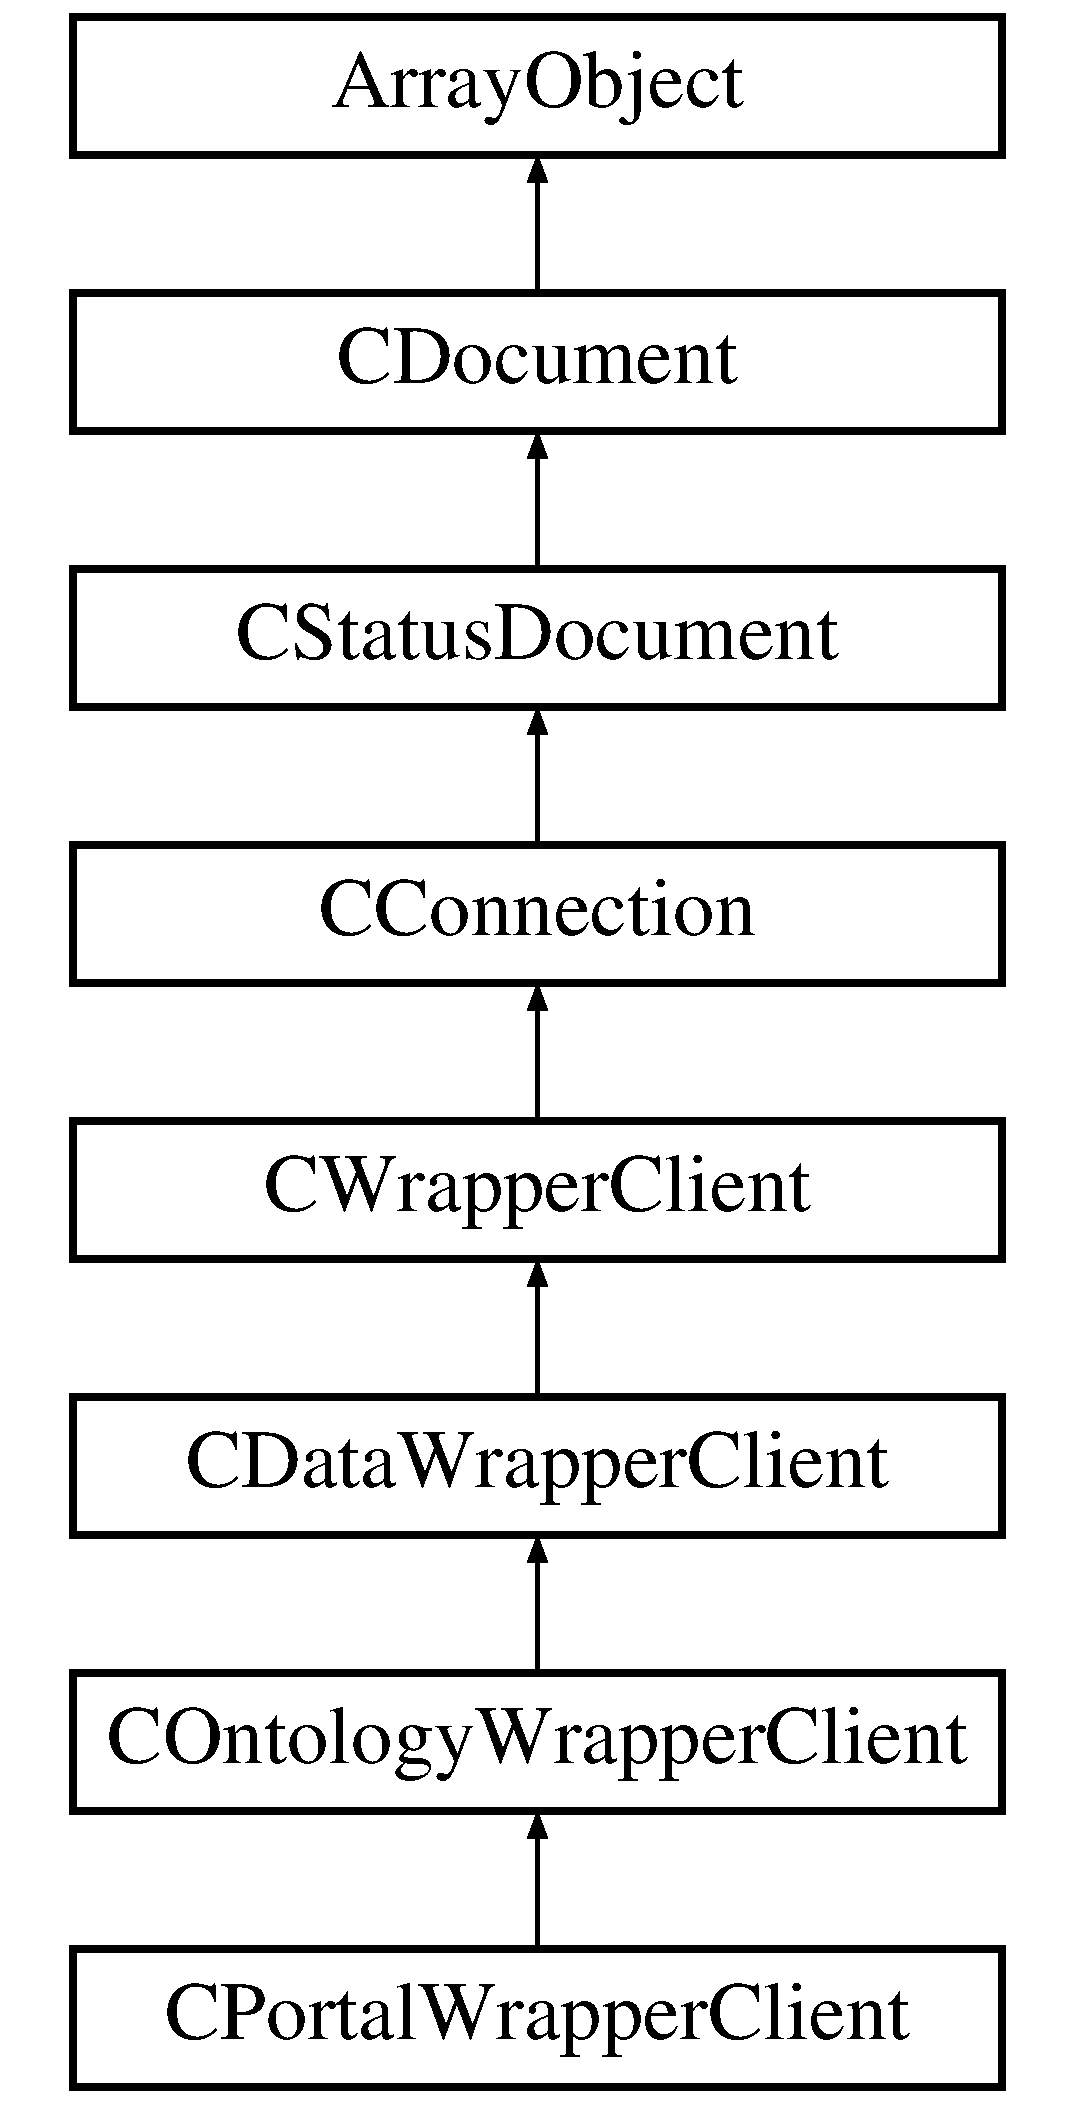
\includegraphics[height=8.000000cm]{class_c_ontology_wrapper_client}
\end{center}
\end{figure}
\subsection*{Public Member Functions}
\begin{DoxyCompactItemize}
\item 
\hyperlink{class_c_ontology_wrapper_client_aca024b449dd2ae6929d189d8f5a1f395}{Operation} (\$the\-Value=N\-U\-L\-L, \$get\-Old=F\-A\-L\-S\-E)
\item 
\hyperlink{class_c_ontology_wrapper_client_a9a9e404e8128831af3baf37497b46ae4}{Query} (\$the\-Value=N\-U\-L\-L, \$get\-Old=F\-A\-L\-S\-E)
\item 
\hyperlink{class_c_ontology_wrapper_client_aacba4e89c53298723dba4ac0a3918e24}{Language} (\$the\-Value=N\-U\-L\-L, \$get\-Old=F\-A\-L\-S\-E)
\item 
\hyperlink{class_c_ontology_wrapper_client_af6922f6f7204b06c6a23eef65260a3b4}{Predicate} (\$the\-Value=N\-U\-L\-L, \$get\-Old=F\-A\-L\-S\-E)
\item 
\hyperlink{class_c_ontology_wrapper_client_a274458fa0b61599f7f936cd48053b5e3}{Relations} (\$the\-Value=N\-U\-L\-L, \$get\-Old=F\-A\-L\-S\-E)
\end{DoxyCompactItemize}
\subsection*{Protected Member Functions}
\begin{DoxyCompactItemize}
\item 
\hyperlink{class_c_ontology_wrapper_client_a5ae9294acc20a820425064f4e7dec7dd}{\-\_\-\-Check\-Dependencies} (\$the\-Operation)
\item 
\hyperlink{class_c_ontology_wrapper_client_a342ff520d30a2ee11ff2ef11a2b532d1}{\-\_\-\-Normalise\-Parameters} ()
\item 
\hyperlink{class_c_ontology_wrapper_client_a8fb7c14b4eb0b9853034236d4f2cbc0f}{\-\_\-\-Encode\-Parameters} (\&\$the\-Parameters, \$the\-Encoding)
\end{DoxyCompactItemize}
\subsection*{Additional Inherited Members}


\subsection{Member Function Documentation}
\hypertarget{class_c_ontology_wrapper_client_a5ae9294acc20a820425064f4e7dec7dd}{\index{C\-Ontology\-Wrapper\-Client@{C\-Ontology\-Wrapper\-Client}!\-\_\-\-Check\-Dependencies@{\-\_\-\-Check\-Dependencies}}
\index{\-\_\-\-Check\-Dependencies@{\-\_\-\-Check\-Dependencies}!COntologyWrapperClient@{C\-Ontology\-Wrapper\-Client}}
\subsubsection[{\-\_\-\-Check\-Dependencies}]{\setlength{\rightskip}{0pt plus 5cm}C\-Ontology\-Wrapper\-Client\-::\-\_\-\-Check\-Dependencies (
\begin{DoxyParamCaption}
\item[{}]{\$the\-Operation}
\end{DoxyParamCaption}
)\hspace{0.3cm}{\ttfamily [protected]}}}\label{class_c_ontology_wrapper_client_a5ae9294acc20a820425064f4e7dec7dd}
Check operation dependencies.

This method can be used to assert whether the required parameters are present depending on the requested operation.


\begin{DoxyParams}[1]{Parameters}
string & {\em \$the\-Operation} & Requested operation.\\
\hline
\end{DoxyParams}
protected


\begin{DoxyExceptions}{Exceptions}
{\em Exception} & \\
\hline
\end{DoxyExceptions}
\hypertarget{class_c_ontology_wrapper_client_a8fb7c14b4eb0b9853034236d4f2cbc0f}{\index{C\-Ontology\-Wrapper\-Client@{C\-Ontology\-Wrapper\-Client}!\-\_\-\-Encode\-Parameters@{\-\_\-\-Encode\-Parameters}}
\index{\-\_\-\-Encode\-Parameters@{\-\_\-\-Encode\-Parameters}!COntologyWrapperClient@{C\-Ontology\-Wrapper\-Client}}
\subsubsection[{\-\_\-\-Encode\-Parameters}]{\setlength{\rightskip}{0pt plus 5cm}C\-Ontology\-Wrapper\-Client\-::\-\_\-\-Encode\-Parameters (
\begin{DoxyParamCaption}
\item[{\&}]{\$the\-Parameters, }
\item[{}]{\$the\-Encoding}
\end{DoxyParamCaption}
)\hspace{0.3cm}{\ttfamily [protected]}}}\label{class_c_ontology_wrapper_client_a8fb7c14b4eb0b9853034236d4f2cbc0f}
Encode parameters.

This method can be used to encode parameters before they get sent to the service.

We overload this method to handle the local parameters.


\begin{DoxyParams}[1]{Parameters}
reference & {\em \&\$the\-Parameters} & List of parameters. \\
\hline
string & {\em \$the\-Encoding} & Encoding code.\\
\hline
\end{DoxyParams}
protected \hypertarget{class_c_ontology_wrapper_client_a342ff520d30a2ee11ff2ef11a2b532d1}{\index{C\-Ontology\-Wrapper\-Client@{C\-Ontology\-Wrapper\-Client}!\-\_\-\-Normalise\-Parameters@{\-\_\-\-Normalise\-Parameters}}
\index{\-\_\-\-Normalise\-Parameters@{\-\_\-\-Normalise\-Parameters}!COntologyWrapperClient@{C\-Ontology\-Wrapper\-Client}}
\subsubsection[{\-\_\-\-Normalise\-Parameters}]{\setlength{\rightskip}{0pt plus 5cm}C\-Ontology\-Wrapper\-Client\-::\-\_\-\-Normalise\-Parameters (
\begin{DoxyParamCaption}
{}
\end{DoxyParamCaption}
)\hspace{0.3cm}{\ttfamily [protected]}}}\label{class_c_ontology_wrapper_client_a342ff520d30a2ee11ff2ef11a2b532d1}
Normalise parameters.

This method can be used to normalise parameters before they get encoded.

In this class we set the request time stamp if the current value is not an float.

In derived classes you should call first the parent method, then handle the local parameters.

protected \hypertarget{class_c_ontology_wrapper_client_aacba4e89c53298723dba4ac0a3918e24}{\index{C\-Ontology\-Wrapper\-Client@{C\-Ontology\-Wrapper\-Client}!Language@{Language}}
\index{Language@{Language}!COntologyWrapperClient@{C\-Ontology\-Wrapper\-Client}}
\subsubsection[{Language}]{\setlength{\rightskip}{0pt plus 5cm}C\-Ontology\-Wrapper\-Client\-::\-Language (
\begin{DoxyParamCaption}
\item[{}]{\$the\-Value = {\ttfamily NULL}, }
\item[{}]{\$get\-Old = {\ttfamily FALSE}}
\end{DoxyParamCaption}
)}}\label{class_c_ontology_wrapper_client_aacba4e89c53298723dba4ac0a3918e24}
Manage language code(s).

This method can be used to manage the \hyperlink{}{k\-A\-P\-I\-\_\-\-L\-A\-N\-G\-U\-A\-G\-E} offset, it accepts a parameter which represents the list of language codes in which \hyperlink{}{k\-T\-Y\-P\-E\-\_\-\-L\-S\-T\-R\-I\-N\-G} attributes are set, or the requested operation, depending on its value\-:


\begin{DoxyItemize}
\item {\itshape N\-U\-L\-L}\-: Return the current value. 
\item {\itshape F\-A\-L\-S\-E}\-: Delete the current value. 
\item {\itshape other}\-: Set the value with the provided parameter, in this case the value is expected to be\-: 
\begin{DoxyItemize}
\item {\ttfamily array} or {\ttfamily Array\-Object{\ttfamily \-: The provided parameter will become the new list. }}
\item {\ttfamily {\ttfamily {\itshape other}\-: The method will assume the parameter is a string and it will add it to the current list or create a list if it doesn't exist. }}
\end{DoxyItemize}
\end{DoxyItemize}

{\ttfamily {\ttfamily The second parameter is a boolean which if {\itshape T\-R\-U\-E} will return the {\itshape old} value when replacing values; if {\itshape F\-A\-L\-S\-E}, it will return the currently set value.}}

{\ttfamily {\ttfamily 
\begin{DoxyParams}[1]{Parameters}
string & {\em \$the\-Value} & Value or operation. \\
\hline
boolean & {\em \$get\-Old} & T\-R\-U\-E get old value.\\
\hline
\end{DoxyParams}
public \begin{DoxyReturn}{Returns}
mixed
\end{DoxyReturn}
\hyperlink{class_c_wrapper_client_a8ad42378b7abfeaaaa311e1b96a42a26}{\-\_\-\-Manage\-List\-Offset()}}}

{\ttfamily {\ttfamily \begin{DoxySeeAlso}{See Also}
k\-A\-P\-I\-\_\-\-L\-A\-N\-G\-U\-A\-G\-E 
\end{DoxySeeAlso}
}}\hypertarget{class_c_ontology_wrapper_client_aca024b449dd2ae6929d189d8f5a1f395}{\index{C\-Ontology\-Wrapper\-Client@{C\-Ontology\-Wrapper\-Client}!Operation@{Operation}}
\index{Operation@{Operation}!COntologyWrapperClient@{C\-Ontology\-Wrapper\-Client}}
\subsubsection[{Operation}]{\setlength{\rightskip}{0pt plus 5cm}C\-Ontology\-Wrapper\-Client\-::\-Operation (
\begin{DoxyParamCaption}
\item[{}]{\$the\-Value = {\ttfamily NULL}, }
\item[{}]{\$get\-Old = {\ttfamily FALSE}}
\end{DoxyParamCaption}
)}}\label{class_c_ontology_wrapper_client_aca024b449dd2ae6929d189d8f5a1f395}
Manage operation.

We \hyperlink{class_c_wrapper_client_ae378229fd57b051ddf0e0a7abf599641}{overload} this method to add the following allowed operations\-:


\begin{DoxyItemize}
\item {\itshape \hyperlink{}{k\-A\-P\-I\-\_\-\-O\-P\-\_\-\-Get\-Vertex}}\-: Return a selection of vertices, or the related vertices of the selected vertex. 
\end{DoxyItemize}


\begin{DoxyParams}[1]{Parameters}
string & {\em \$the\-Value} & Value or operation. \\
\hline
boolean & {\em \$get\-Old} & T\-R\-U\-E get old value.\\
\hline
\end{DoxyParams}
public \begin{DoxyReturn}{Returns}
mixed
\end{DoxyReturn}

\begin{DoxyExceptions}{Exceptions}
{\em \{@link} & \hyperlink{class_c_exception}{C\-Exception} \hyperlink{class_c_exception}{C\-Exception}\}\\
\hline
\end{DoxyExceptions}
C\-Attribute\-::\-Manage\-Offset()

\begin{DoxySeeAlso}{See Also}
k\-A\-P\-I\-\_\-\-O\-P\-E\-R\-A\-T\-I\-O\-N 

k\-A\-P\-I\-\_\-\-O\-P\-\_\-\-Get\-Vertex 
\end{DoxySeeAlso}
\hypertarget{class_c_ontology_wrapper_client_af6922f6f7204b06c6a23eef65260a3b4}{\index{C\-Ontology\-Wrapper\-Client@{C\-Ontology\-Wrapper\-Client}!Predicate@{Predicate}}
\index{Predicate@{Predicate}!COntologyWrapperClient@{C\-Ontology\-Wrapper\-Client}}
\subsubsection[{Predicate}]{\setlength{\rightskip}{0pt plus 5cm}C\-Ontology\-Wrapper\-Client\-::\-Predicate (
\begin{DoxyParamCaption}
\item[{}]{\$the\-Value = {\ttfamily NULL}, }
\item[{}]{\$get\-Old = {\ttfamily FALSE}}
\end{DoxyParamCaption}
)}}\label{class_c_ontology_wrapper_client_af6922f6f7204b06c6a23eef65260a3b4}
Manage predicate(s) selector.

This method can be used to manage the \hyperlink{}{k\-A\-P\-I\-\_\-\-P\-R\-E\-D\-I\-C\-A\-T\-E} offset, it accepts a parameter which represents the list of predicate references, or the requested operation, depending on its value\-:


\begin{DoxyItemize}
\item {\itshape N\-U\-L\-L}\-: Return the current value. 
\item {\itshape F\-A\-L\-S\-E}\-: Delete the current value. 
\item {\itshape other}\-: Set the value with the provided parameter, in this case the value is expected to be\-: 
\begin{DoxyItemize}
\item {\ttfamily array} or {\ttfamily Array\-Object{\ttfamily \-: The provided parameter will become the new list. }}
\item {\ttfamily {\ttfamily {\itshape other}\-: The method will assume the parameter is a string and it will add it to the current list or create a list if it doesn't exist. }}
\end{DoxyItemize}
\end{DoxyItemize}

{\ttfamily {\ttfamily The second parameter is a boolean which if {\itshape T\-R\-U\-E} will return the {\itshape old} value when replacing values; if {\itshape F\-A\-L\-S\-E}, it will return the currently set value.}}

{\ttfamily {\ttfamily 
\begin{DoxyParams}[1]{Parameters}
string & {\em \$the\-Value} & Value or operation. \\
\hline
boolean & {\em \$get\-Old} & T\-R\-U\-E get old value.\\
\hline
\end{DoxyParams}
public \begin{DoxyReturn}{Returns}
mixed
\end{DoxyReturn}
\hyperlink{class_c_wrapper_client_a8ad42378b7abfeaaaa311e1b96a42a26}{\-\_\-\-Manage\-List\-Offset()}}}

{\ttfamily {\ttfamily \begin{DoxySeeAlso}{See Also}
k\-A\-P\-I\-\_\-\-P\-R\-E\-D\-I\-C\-A\-T\-E 
\end{DoxySeeAlso}
}}\hypertarget{class_c_ontology_wrapper_client_a9a9e404e8128831af3baf37497b46ae4}{\index{C\-Ontology\-Wrapper\-Client@{C\-Ontology\-Wrapper\-Client}!Query@{Query}}
\index{Query@{Query}!COntologyWrapperClient@{C\-Ontology\-Wrapper\-Client}}
\subsubsection[{Query}]{\setlength{\rightskip}{0pt plus 5cm}C\-Ontology\-Wrapper\-Client\-::\-Query (
\begin{DoxyParamCaption}
\item[{}]{\$the\-Value = {\ttfamily NULL}, }
\item[{}]{\$get\-Old = {\ttfamily FALSE}}
\end{DoxyParamCaption}
)}}\label{class_c_ontology_wrapper_client_a9a9e404e8128831af3baf37497b46ae4}
Manage query.

We overload this method to allow setting the query directly with the vertex identifier, if the method argument is an integer, we assume the value is a node native identifier and we set the query to match it.


\begin{DoxyParams}[1]{Parameters}
string & {\em \$the\-Value} & Value or operation. \\
\hline
boolean & {\em \$get\-Old} & T\-R\-U\-E get old value.\\
\hline
\end{DoxyParams}
public \begin{DoxyReturn}{Returns}
mixed
\end{DoxyReturn}

\begin{DoxyExceptions}{Exceptions}
{\em Exception} & Manage\-Offset()\\
\hline
\end{DoxyExceptions}
\begin{DoxySeeAlso}{See Also}
k\-A\-P\-I\-\_\-\-Q\-U\-E\-R\-Y 
\end{DoxySeeAlso}
\hypertarget{class_c_ontology_wrapper_client_a274458fa0b61599f7f936cd48053b5e3}{\index{C\-Ontology\-Wrapper\-Client@{C\-Ontology\-Wrapper\-Client}!Relations@{Relations}}
\index{Relations@{Relations}!COntologyWrapperClient@{C\-Ontology\-Wrapper\-Client}}
\subsubsection[{Relations}]{\setlength{\rightskip}{0pt plus 5cm}C\-Ontology\-Wrapper\-Client\-::\-Relations (
\begin{DoxyParamCaption}
\item[{}]{\$the\-Value = {\ttfamily NULL}, }
\item[{}]{\$get\-Old = {\ttfamily FALSE}}
\end{DoxyParamCaption}
)}}\label{class_c_ontology_wrapper_client_a274458fa0b61599f7f936cd48053b5e3}
Manage relationships sense.

This method can be used to manage the \hyperlink{}{k\-A\-P\-I\-\_\-\-R\-E\-L\-A\-T\-I\-O\-N} offset, it accepts a parameter which represents the relationships sense, or the requested operation, depending on its value\-:


\begin{DoxyItemize}
\item {\ttfamily N\-U\-L\-L}\-: Return the current value. 
\item {\ttfamily F\-A\-L\-S\-E}\-: Delete the current value. 
\item {\ttfamily \hyperlink{}{k\-A\-P\-I\-\_\-\-R\-E\-L\-A\-T\-I\-O\-N\-\_\-\-I\-N}}\-: Incoming relationships. 
\item {\ttfamily \hyperlink{}{k\-A\-P\-I\-\_\-\-R\-E\-L\-A\-T\-I\-O\-N\-\_\-\-O\-U\-T}}\-: Outgoing relationships. 
\item {\ttfamily \hyperlink{}{k\-A\-P\-I\-\_\-\-R\-E\-L\-A\-T\-I\-O\-N\-\_\-\-A\-L\-L}}\-: Incoming and outgoing relationships. 
\item {\itshape other}\-: The method will raise an exception. 
\end{DoxyItemize}

The second parameter is a boolean which if {\itshape T\-R\-U\-E} will return the {\itshape old} value when replacing values; if {\itshape F\-A\-L\-S\-E}, it will return the currently set value.


\begin{DoxyParams}[1]{Parameters}
string & {\em \$the\-Value} & Value or operation. \\
\hline
boolean & {\em \$get\-Old} & T\-R\-U\-E get old value.\\
\hline
\end{DoxyParams}
public \begin{DoxyReturn}{Returns}
mixed
\end{DoxyReturn}
Manage\-Offset()

\begin{DoxySeeAlso}{See Also}
k\-A\-P\-I\-\_\-\-R\-E\-L\-A\-T\-I\-O\-N 
\end{DoxySeeAlso}


The documentation for this class was generated from the following file\-:\begin{DoxyCompactItemize}
\item 
/\-Library/\-Web\-Server/\-Library/\-P\-H\-P\-Wrapper/classes/C\-Ontology\-Wrapper\-Client.\-php\end{DoxyCompactItemize}

\hypertarget{class_c_persistent_document}{\section{C\-Persistent\-Document Class Reference}
\label{class_c_persistent_document}\index{C\-Persistent\-Document@{C\-Persistent\-Document}}
}
Inheritance diagram for C\-Persistent\-Document\-:\begin{figure}[H]
\begin{center}
\leavevmode
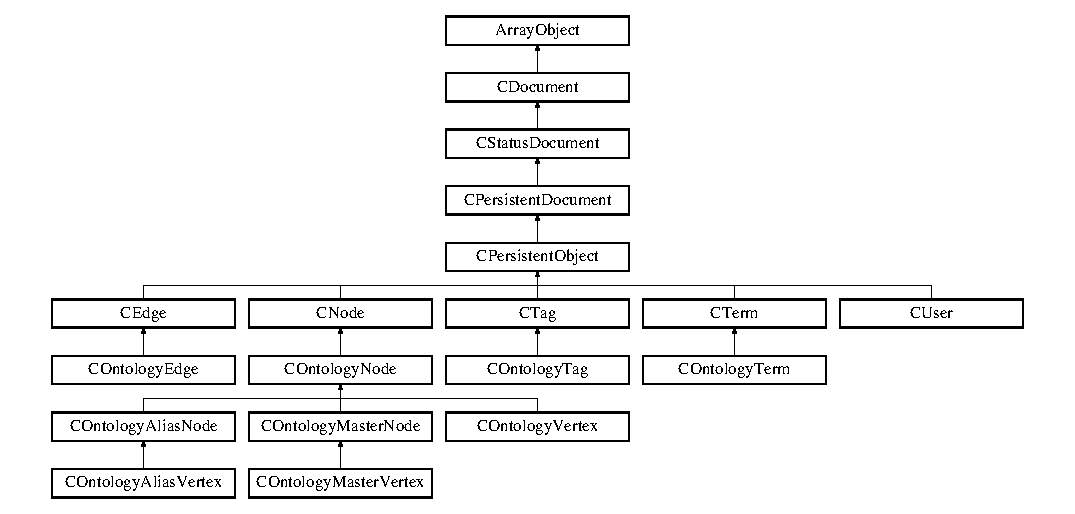
\includegraphics[height=6.461539cm]{class_c_persistent_document}
\end{center}
\end{figure}
\subsection*{Public Member Functions}
\begin{DoxyCompactItemize}
\item 
\hyperlink{class_c_persistent_document_ad9d15abc074aa3f779f214771b6123b0}{N\-I\-D} (\$the\-Value=N\-U\-L\-L, \$get\-Old=F\-A\-L\-S\-E)
\item 
\hyperlink{class_c_persistent_document_a3b3a1168053b14b065e11caad44dc971}{Insert} (\hyperlink{class_c_connection}{C\-Connection} \$the\-Connection)
\item 
\hyperlink{class_c_persistent_document_ae0435275b85d3d3fa6eb76711e0f0832}{Update} (\hyperlink{class_c_connection}{C\-Connection} \$the\-Connection)
\item 
\hyperlink{class_c_persistent_document_a1a3fb046a36fec064fca7cacdcc6cb3e}{Replace} (\hyperlink{class_c_connection}{C\-Connection} \$the\-Connection)
\item 
\hyperlink{class_c_persistent_document_a19f7dbe659a1174d844799e403d1a678}{Restore} (\hyperlink{class_c_connection}{C\-Connection} \$the\-Connection)
\item 
\hyperlink{class_c_persistent_document_a7ea1235ae140507d9fc0f94b6060540c}{Delete} (\hyperlink{class_c_connection}{C\-Connection} \$the\-Connection)
\end{DoxyCompactItemize}
\subsection*{Static Public Member Functions}
\begin{DoxyCompactItemize}
\item 
static \hyperlink{class_c_persistent_document_afdb58ccaae70ff12ad424fd841f23fe9}{New\-Object} (\hyperlink{class_c_connection}{C\-Connection} \$the\-Connection, \$the\-Identifier, \$do\-Throw=F\-A\-L\-S\-E)
\item 
static \hyperlink{class_c_persistent_document_a6092e640e36485873b70a79db464e0ff}{Default\-Database} (\hyperlink{class_c_server}{C\-Server} \$the\-Server)
\item 
static \hyperlink{class_c_persistent_document_a031b386207e40e4be4e0660de5da1b11}{Default\-Database\-Name} ()
\item 
static \hyperlink{class_c_persistent_document_ada019252d242b5a88a26b82a18e29ed6}{Default\-Container} (\hyperlink{class_c_database}{C\-Database} \$the\-Database)
\item 
static \hyperlink{class_c_persistent_document_ab2fa5e1b0e3f967b8b3727eb28300652}{Default\-Container\-Name} ()
\item 
static \hyperlink{class_c_persistent_document_a4dbe287aa3b46bdc0a1157e001078589}{Resolve\-Container} (\hyperlink{class_c_connection}{C\-Connection} \$the\-Connection, \$do\-Exception)
\item 
static \hyperlink{class_c_persistent_document_ac6a46b4cfed5f22ec63a6436a107ed69}{Resolve\-Class\-Container} (\hyperlink{class_c_connection}{C\-Connection} \$the\-Connection, \$do\-Exception)
\end{DoxyCompactItemize}
\subsection*{Protected Member Functions}
\begin{DoxyCompactItemize}
\item 
\hyperlink{class_c_persistent_document_a23cfbb5ebf75e008622ab9e723472c70}{\-\_\-\-Precommit} (\hyperlink{class_c_connection}{C\-Connection} \$the\-Connection, \$the\-Modifiers=k\-F\-L\-A\-G\-\_\-\-D\-E\-F\-A\-U\-L\-T)
\item 
\hyperlink{class_c_persistent_document_aa7fdfe47ee3099ebda49a76e1fa24670}{\-\_\-\-Postcommit} (\hyperlink{class_c_connection}{C\-Connection} \$the\-Connection, \$the\-Modifiers=k\-F\-L\-A\-G\-\_\-\-D\-E\-F\-A\-U\-L\-T)
\item 
\hyperlink{class_c_persistent_document_afdf23fd212084711a4c6357e335c3214}{\-\_\-\-Precommit\-Validate} (\&\$the\-Connection, \&\$the\-Modifiers)
\item 
\hyperlink{class_c_persistent_document_a432319392179e142ed03919b9eddc30e}{\-\_\-\-Precommit\-Related} (\&\$the\-Connection, \&\$the\-Modifiers)
\item 
\hyperlink{class_c_persistent_document_aff5680d29ebcbc9fce715270759a95cd}{\-\_\-\-Precommit\-Identify} (\&\$the\-Connection, \&\$the\-Modifiers)
\item 
\hyperlink{class_c_persistent_document_a7772771f349b5d9d4dbc192ce7c8a012}{\-\_\-\-Postcommit\-Related} (\&\$the\-Connection, \&\$the\-Modifiers)
\item 
\hyperlink{class_c_persistent_document_a774c94863383129a0813ee15a4cb76dd}{\-\_\-\-Postcommit\-Status} (\&\$the\-Connection, \&\$the\-Modifiers)
\item 
\hyperlink{class_c_persistent_document_a649e5b01c3e3c2d9ab0d99cff6b3349f}{\-\_\-\-Postcommit\-Cleanup} (\&\$the\-Connection, \&\$the\-Modifiers)
\end{DoxyCompactItemize}
\subsection*{Additional Inherited Members}


\subsection{Member Function Documentation}
\hypertarget{class_c_persistent_document_aa7fdfe47ee3099ebda49a76e1fa24670}{\index{C\-Persistent\-Document@{C\-Persistent\-Document}!\-\_\-\-Postcommit@{\-\_\-\-Postcommit}}
\index{\-\_\-\-Postcommit@{\-\_\-\-Postcommit}!CPersistentDocument@{C\-Persistent\-Document}}
\subsubsection[{\-\_\-\-Postcommit}]{\setlength{\rightskip}{0pt plus 5cm}C\-Persistent\-Document\-::\-\_\-\-Postcommit (
\begin{DoxyParamCaption}
\item[{{\bf C\-Connection}}]{\$the\-Connection, }
\item[{}]{\$the\-Modifiers = {\ttfamily kFLAG\-\_\-DEFAULT}}
\end{DoxyParamCaption}
)\hspace{0.3cm}{\ttfamily [protected]}}}\label{class_c_persistent_document_aa7fdfe47ee3099ebda49a76e1fa24670}
\subparagraph*{Prepare the object after committing}

This method will be called after the object gets committed, its main duty is to update the object after it has been committed.

This method calls three other methods which perform the following functions\-:


\begin{DoxyItemize}
\item \hyperlink{class_c_persistent_document_a7772771f349b5d9d4dbc192ce7c8a012}{\-\_\-\-Postcommit\-Related()}\-: This method's duty is to update related objects. 
\item \hyperlink{class_c_persistent_document_a774c94863383129a0813ee15a4cb76dd}{\-\_\-\-Postcommit\-Status()}\-: This method's duty is to set the object's status after the persist operation. 
\item \hyperlink{class_c_persistent_document_a649e5b01c3e3c2d9ab0d99cff6b3349f}{\-\_\-\-Postcommit\-Cleanup()}\-: This method's duty is to cleanup the object after the operation. 
\end{DoxyItemize}

These three methods are called in the above order, they take the same arguments as the current method and do not return a value\-: errors must raise exceptions.

When deriving from this class you should overload the above methods and not this one.

This method accepts two parameters\-:


\begin{DoxyItemize}
\item {\ttfamily \$the\-Connection}\-: The container in which the object is to be committed, a server or a database if the \hyperlink{class_c_persistent_document_a6092e640e36485873b70a79db464e0ff}{Default\-Database} and \hyperlink{class_c_persistent_document_ada019252d242b5a88a26b82a18e29ed6}{Default\-Container()} are able to resolve it into a container. 
\item {\ttfamily \$the\-Modifiers}\-: The commit options provided as a bitfield in which the following values are considered\-: 
\begin{DoxyItemize}
\item {\ttfamily \hyperlink{}{k\-F\-L\-A\-G\-\_\-\-P\-E\-R\-S\-I\-S\-T\-\_\-\-I\-N\-S\-E\-R\-T}}\-: Insert operation. 
\item {\ttfamily \hyperlink{}{k\-F\-L\-A\-G\-\_\-\-P\-E\-R\-S\-I\-S\-T\-\_\-\-U\-P\-D\-A\-T\-E}}\-: Update operation. 
\item {\ttfamily \hyperlink{}{k\-F\-L\-A\-G\-\_\-\-P\-E\-R\-S\-I\-S\-T\-\_\-\-R\-E\-P\-L\-A\-C\-E}}\-: Replace operation. 
\item {\ttfamily \hyperlink{}{k\-F\-L\-A\-G\-\_\-\-P\-E\-R\-S\-I\-S\-T\-\_\-\-D\-E\-L\-E\-T\-E}}\-: Delete operation. 
\end{DoxyItemize}
\end{DoxyItemize}


\begin{DoxyParams}[1]{Parameters}
\hyperlink{class_c_connection}{C\-Connection} & {\em \$the\-Connection} & Container. \\
\hline
bitfield & {\em \$the\-Modifiers} & Commit options.\\
\hline
\end{DoxyParams}
protected

\hyperlink{class_c_persistent_document_a7772771f349b5d9d4dbc192ce7c8a012}{\-\_\-\-Postcommit\-Related()}  \hyperlink{class_c_persistent_document_a774c94863383129a0813ee15a4cb76dd}{\-\_\-\-Postcommit\-Status()}  \hyperlink{class_c_persistent_document_a649e5b01c3e3c2d9ab0d99cff6b3349f}{\-\_\-\-Postcommit\-Cleanup()} \hypertarget{class_c_persistent_document_a649e5b01c3e3c2d9ab0d99cff6b3349f}{\index{C\-Persistent\-Document@{C\-Persistent\-Document}!\-\_\-\-Postcommit\-Cleanup@{\-\_\-\-Postcommit\-Cleanup}}
\index{\-\_\-\-Postcommit\-Cleanup@{\-\_\-\-Postcommit\-Cleanup}!CPersistentDocument@{C\-Persistent\-Document}}
\subsubsection[{\-\_\-\-Postcommit\-Cleanup}]{\setlength{\rightskip}{0pt plus 5cm}C\-Persistent\-Document\-::\-\_\-\-Postcommit\-Cleanup (
\begin{DoxyParamCaption}
\item[{\&}]{\$the\-Connection, }
\item[{\&}]{\$the\-Modifiers}
\end{DoxyParamCaption}
)\hspace{0.3cm}{\ttfamily [protected]}}}\label{class_c_persistent_document_a649e5b01c3e3c2d9ab0d99cff6b3349f}
\subparagraph*{Cleanup the object after committing}

This method should clean and normalise the object after the operation, it is the last method called by \hyperlink{class_c_persistent_document_aa7fdfe47ee3099ebda49a76e1fa24670}{\-\_\-\-Postcommit()} and the last chance to have a hook into the persist workflow.

Be aware that \hyperlink{class_c_persistent_document_a774c94863383129a0813ee15a4cb76dd}{\-\_\-\-Postcommit\-Status()} has been called before, so if you intend to perform operations that may change the object's status, this is not the place.

The method accepts two parameters\-:


\begin{DoxyItemize}
\item {\ttfamily \$the\-Connection}\-: The container in which the object is to be committed, a server or a database if the \hyperlink{class_c_persistent_document_a6092e640e36485873b70a79db464e0ff}{Default\-Database} and \hyperlink{class_c_persistent_document_ada019252d242b5a88a26b82a18e29ed6}{Default\-Container()} are able to resolve it into a container. This parameter is provided as a reference allowing this method to change it. 
\item {\ttfamily \$the\-Modifiers}\-: The commit options provided as a bitfield in which the following values are considered\-: 
\begin{DoxyItemize}
\item {\ttfamily \hyperlink{}{k\-F\-L\-A\-G\-\_\-\-P\-E\-R\-S\-I\-S\-T\-\_\-\-I\-N\-S\-E\-R\-T}}\-: Insert operation. 
\item {\ttfamily \hyperlink{}{k\-F\-L\-A\-G\-\_\-\-P\-E\-R\-S\-I\-S\-T\-\_\-\-U\-P\-D\-A\-T\-E}}\-: Update operation. 
\item {\ttfamily \hyperlink{}{k\-F\-L\-A\-G\-\_\-\-P\-E\-R\-S\-I\-S\-T\-\_\-\-R\-E\-P\-L\-A\-C\-E}}\-: Replace operation. 
\item {\ttfamily \hyperlink{}{k\-F\-L\-A\-G\-\_\-\-P\-E\-R\-S\-I\-S\-T\-\_\-\-D\-E\-L\-E\-T\-E}}\-: Delete operation. 
\end{DoxyItemize}This parameter is provided as a reference allowing this method to change it. 
\end{DoxyItemize}

In this class we reset the \hyperlink{class_c_status_document_ad5193995e1bff6de09acf3248a232ef9}{\-\_\-\-Is\-Dirty()} status after committing or loading the object, set the \hyperlink{class_c_status_document_ab7d96fd4588cf7d5432fc65a1d1fb076}{\-\_\-\-Is\-Committed()} status after committing and resetting it after deleting.

In this class we do nothing.


\begin{DoxyParams}[1]{Parameters}
reference & {\em \&\$the\-Connection} & Server, database or container. \\
\hline
reference & {\em \&\$the\-Modifiers} & Commit options.\\
\hline
\end{DoxyParams}
protected \hypertarget{class_c_persistent_document_a7772771f349b5d9d4dbc192ce7c8a012}{\index{C\-Persistent\-Document@{C\-Persistent\-Document}!\-\_\-\-Postcommit\-Related@{\-\_\-\-Postcommit\-Related}}
\index{\-\_\-\-Postcommit\-Related@{\-\_\-\-Postcommit\-Related}!CPersistentDocument@{C\-Persistent\-Document}}
\subsubsection[{\-\_\-\-Postcommit\-Related}]{\setlength{\rightskip}{0pt plus 5cm}C\-Persistent\-Document\-::\-\_\-\-Postcommit\-Related (
\begin{DoxyParamCaption}
\item[{\&}]{\$the\-Connection, }
\item[{\&}]{\$the\-Modifiers}
\end{DoxyParamCaption}
)\hspace{0.3cm}{\ttfamily [protected]}}}\label{class_c_persistent_document_a7772771f349b5d9d4dbc192ce7c8a012}
\subparagraph*{Update related objects after committing}

This method should update eventual related objects after the current object has been committed. This method is the first one called by \hyperlink{class_c_persistent_document_aa7fdfe47ee3099ebda49a76e1fa24670}{\-\_\-\-Postcommit()} after the persist operation and the object has not yet updated its status according to the operation, so this is a good place to make changes before the status gets reset.

The method accepts two parameters\-:


\begin{DoxyItemize}
\item {\ttfamily \$the\-Connection}\-: The container in which the object is to be committed, a server or a database if the \hyperlink{class_c_persistent_document_a6092e640e36485873b70a79db464e0ff}{Default\-Database} and \hyperlink{class_c_persistent_document_ada019252d242b5a88a26b82a18e29ed6}{Default\-Container()} are able to resolve it into a container. This parameter is provided as a reference allowing this method to change it. 
\item {\ttfamily \$the\-Modifiers}\-: The commit options provided as a bitfield in which the following values are considered\-: 
\begin{DoxyItemize}
\item {\ttfamily \hyperlink{}{k\-F\-L\-A\-G\-\_\-\-P\-E\-R\-S\-I\-S\-T\-\_\-\-I\-N\-S\-E\-R\-T}}\-: Insert operation. 
\item {\ttfamily \hyperlink{}{k\-F\-L\-A\-G\-\_\-\-P\-E\-R\-S\-I\-S\-T\-\_\-\-U\-P\-D\-A\-T\-E}}\-: Update operation. 
\item {\ttfamily \hyperlink{}{k\-F\-L\-A\-G\-\_\-\-P\-E\-R\-S\-I\-S\-T\-\_\-\-R\-E\-P\-L\-A\-C\-E}}\-: Replace operation. 
\item {\ttfamily \hyperlink{}{k\-F\-L\-A\-G\-\_\-\-P\-E\-R\-S\-I\-S\-T\-\_\-\-D\-E\-L\-E\-T\-E}}\-: Delete operation. 
\end{DoxyItemize}This parameter is provided as a reference allowing this method to change it. 
\end{DoxyItemize}

In this class we do nothing.


\begin{DoxyParams}[1]{Parameters}
reference & {\em \&\$the\-Connection} & Server, database or container. \\
\hline
reference & {\em \&\$the\-Modifiers} & Commit options.\\
\hline
\end{DoxyParams}
protected \hypertarget{class_c_persistent_document_a774c94863383129a0813ee15a4cb76dd}{\index{C\-Persistent\-Document@{C\-Persistent\-Document}!\-\_\-\-Postcommit\-Status@{\-\_\-\-Postcommit\-Status}}
\index{\-\_\-\-Postcommit\-Status@{\-\_\-\-Postcommit\-Status}!CPersistentDocument@{C\-Persistent\-Document}}
\subsubsection[{\-\_\-\-Postcommit\-Status}]{\setlength{\rightskip}{0pt plus 5cm}C\-Persistent\-Document\-::\-\_\-\-Postcommit\-Status (
\begin{DoxyParamCaption}
\item[{\&}]{\$the\-Connection, }
\item[{\&}]{\$the\-Modifiers}
\end{DoxyParamCaption}
)\hspace{0.3cm}{\ttfamily [protected]}}}\label{class_c_persistent_document_a774c94863383129a0813ee15a4cb76dd}
\subparagraph*{Update the object's status after committing}

This method should set the object status according to the operation performed, it is the second method called by \hyperlink{class_c_persistent_document_aa7fdfe47ee3099ebda49a76e1fa24670}{\-\_\-\-Postcommit()} after the persist operation and is called before the \hyperlink{class_c_persistent_document_a649e5b01c3e3c2d9ab0d99cff6b3349f}{\-\_\-\-Postcommit\-Cleanup()} method that should cleanup after the operation.

In general this method should set or reset the status reflecting the persistent state of the object.

The method accepts two parameters\-:


\begin{DoxyItemize}
\item {\ttfamily \$the\-Connection}\-: The container in which the object is to be committed, a server or a database if the \hyperlink{class_c_persistent_document_a6092e640e36485873b70a79db464e0ff}{Default\-Database} and \hyperlink{class_c_persistent_document_ada019252d242b5a88a26b82a18e29ed6}{Default\-Container()} are able to resolve it into a container. This parameter is provided as a reference allowing this method to change it. 
\item {\ttfamily \$the\-Modifiers}\-: The commit options provided as a bitfield in which the following values are considered\-: 
\begin{DoxyItemize}
\item {\ttfamily \hyperlink{}{k\-F\-L\-A\-G\-\_\-\-P\-E\-R\-S\-I\-S\-T\-\_\-\-I\-N\-S\-E\-R\-T}}\-: Insert operation. 
\item {\ttfamily \hyperlink{}{k\-F\-L\-A\-G\-\_\-\-P\-E\-R\-S\-I\-S\-T\-\_\-\-U\-P\-D\-A\-T\-E}}\-: Update operation. 
\item {\ttfamily \hyperlink{}{k\-F\-L\-A\-G\-\_\-\-P\-E\-R\-S\-I\-S\-T\-\_\-\-R\-E\-P\-L\-A\-C\-E}}\-: Replace operation. 
\item {\ttfamily \hyperlink{}{k\-F\-L\-A\-G\-\_\-\-P\-E\-R\-S\-I\-S\-T\-\_\-\-D\-E\-L\-E\-T\-E}}\-: Delete operation. 
\end{DoxyItemize}This parameter is provided as a reference allowing this method to change it. 
\end{DoxyItemize}

In this class we reset the \hyperlink{class_c_status_document_ad5193995e1bff6de09acf3248a232ef9}{\-\_\-\-Is\-Dirty()} status after committing or loading the object, set the \hyperlink{class_c_status_document_ab7d96fd4588cf7d5432fc65a1d1fb076}{\-\_\-\-Is\-Committed()} status after committing and resetting it after deleting.


\begin{DoxyParams}[1]{Parameters}
reference & {\em \&\$the\-Connection} & Server, database or container. \\
\hline
reference & {\em \&\$the\-Modifiers} & Commit options.\\
\hline
\end{DoxyParams}
protected

\hyperlink{class_c_status_document_ad5193995e1bff6de09acf3248a232ef9}{\-\_\-\-Is\-Dirty()}  \hyperlink{class_c_status_document_ab7d96fd4588cf7d5432fc65a1d1fb076}{\-\_\-\-Is\-Committed()}

\begin{DoxySeeAlso}{See Also}
k\-F\-L\-A\-G\-\_\-\-P\-E\-R\-S\-I\-S\-T\-\_\-\-M\-A\-S\-K k\-F\-L\-A\-G\-\_\-\-P\-E\-R\-S\-I\-S\-T\-\_\-\-C\-O\-M\-M\-I\-T\-\_\-\-M\-A\-S\-K k\-F\-L\-A\-G\-\_\-\-P\-E\-R\-S\-I\-S\-T\-\_\-\-D\-E\-L\-E\-T\-E 
\end{DoxySeeAlso}
\hypertarget{class_c_persistent_document_a23cfbb5ebf75e008622ab9e723472c70}{\index{C\-Persistent\-Document@{C\-Persistent\-Document}!\-\_\-\-Precommit@{\-\_\-\-Precommit}}
\index{\-\_\-\-Precommit@{\-\_\-\-Precommit}!CPersistentDocument@{C\-Persistent\-Document}}
\subsubsection[{\-\_\-\-Precommit}]{\setlength{\rightskip}{0pt plus 5cm}C\-Persistent\-Document\-::\-\_\-\-Precommit (
\begin{DoxyParamCaption}
\item[{{\bf C\-Connection}}]{\$the\-Connection, }
\item[{}]{\$the\-Modifiers = {\ttfamily kFLAG\-\_\-DEFAULT}}
\end{DoxyParamCaption}
)\hspace{0.3cm}{\ttfamily [protected]}}}\label{class_c_persistent_document_a23cfbb5ebf75e008622ab9e723472c70}
\subparagraph*{Prepare the object before committing}

This method will be called before the object gets committed, its main duty is to check whether the object has all the required elements, to set all default data amd to commit eventual embedded objects.

This method calls three other methods which perform the following functions\-:


\begin{DoxyItemize}
\item \hyperlink{class_c_persistent_document_afdf23fd212084711a4c6357e335c3214}{\-\_\-\-Precommit\-Validate()}\-: This method's duty is to check if the object is fot for being committed. 
\item \hyperlink{class_c_persistent_document_a432319392179e142ed03919b9eddc30e}{\-\_\-\-Precommit\-Related()}\-: This method's duty is to check and commit eventual embedded or related objects. 
\item \hyperlink{class_c_persistent_document_aff5680d29ebcbc9fce715270759a95cd}{\-\_\-\-Precommit\-Identify()}\-: This method's duty is to fill the object's identifiers. 
\end{DoxyItemize}

These three methods are called in the above order, they take the same arguments as the current method. These methods may return two kind of values\-:


\begin{DoxyItemize}
\item {\ttfamily N\-U\-L\-L}\-: This value indicates that everything should continue as planned. 
\item {\itshape other}\-: Any other value is interpreted as the object's native identifier, this is an indication that the object was committed and that the calling method can directly return this value. 
\end{DoxyItemize}

When deriving from this class you should overload the above methods and not this one.

This method accepts two parameters\-:


\begin{DoxyItemize}
\item {\ttfamily \$the\-Connection}\-: The container in which the object is to be committed, a server or a database if the \hyperlink{class_c_persistent_document_a6092e640e36485873b70a79db464e0ff}{Default\-Database} and \hyperlink{class_c_persistent_document_ada019252d242b5a88a26b82a18e29ed6}{Default\-Container()} are able to resolve it into a container. 
\item {\ttfamily \$the\-Modifiers}\-: The commit options provided as a bitfield in which the following values are considered\-: 
\begin{DoxyItemize}
\item {\ttfamily \hyperlink{}{k\-F\-L\-A\-G\-\_\-\-P\-E\-R\-S\-I\-S\-T\-\_\-\-I\-N\-S\-E\-R\-T}}\-: Insert operation. 
\item {\ttfamily \hyperlink{}{k\-F\-L\-A\-G\-\_\-\-P\-E\-R\-S\-I\-S\-T\-\_\-\-U\-P\-D\-A\-T\-E}}\-: Update operation. 
\item {\ttfamily \hyperlink{}{k\-F\-L\-A\-G\-\_\-\-P\-E\-R\-S\-I\-S\-T\-\_\-\-R\-E\-P\-L\-A\-C\-E}}\-: Replace operation. 
\item {\ttfamily \hyperlink{}{k\-F\-L\-A\-G\-\_\-\-P\-E\-R\-S\-I\-S\-T\-\_\-\-D\-E\-L\-E\-T\-E}}\-: Delete operation. 
\end{DoxyItemize}
\end{DoxyItemize}

If the conditions for committing the object are not met, an exception should be raised.


\begin{DoxyParams}[1]{Parameters}
\hyperlink{class_c_connection}{C\-Connection} & {\em \$the\-Connection} & Container. \\
\hline
bitfield & {\em \$the\-Modifiers} & Commit options.\\
\hline
\end{DoxyParams}
protected \begin{DoxyReturn}{Returns}
mixed
\end{DoxyReturn}
\hyperlink{class_c_persistent_document_afdf23fd212084711a4c6357e335c3214}{\-\_\-\-Precommit\-Validate()}  \hyperlink{class_c_persistent_document_a432319392179e142ed03919b9eddc30e}{\-\_\-\-Precommit\-Related()}  \hyperlink{class_c_persistent_document_aff5680d29ebcbc9fce715270759a95cd}{\-\_\-\-Precommit\-Identify()} \hypertarget{class_c_persistent_document_aff5680d29ebcbc9fce715270759a95cd}{\index{C\-Persistent\-Document@{C\-Persistent\-Document}!\-\_\-\-Precommit\-Identify@{\-\_\-\-Precommit\-Identify}}
\index{\-\_\-\-Precommit\-Identify@{\-\_\-\-Precommit\-Identify}!CPersistentDocument@{C\-Persistent\-Document}}
\subsubsection[{\-\_\-\-Precommit\-Identify}]{\setlength{\rightskip}{0pt plus 5cm}C\-Persistent\-Document\-::\-\_\-\-Precommit\-Identify (
\begin{DoxyParamCaption}
\item[{\&}]{\$the\-Connection, }
\item[{\&}]{\$the\-Modifiers}
\end{DoxyParamCaption}
)\hspace{0.3cm}{\ttfamily [protected]}}}\label{class_c_persistent_document_aff5680d29ebcbc9fce715270759a95cd}
\subparagraph*{Determine the identifiers before committing}

This method should set the object identifiers before the current object gets committed. In general it is here where you set sequence numbers or generate unique identifiers.

This method is the last one called by \hyperlink{class_c_persistent_document_a23cfbb5ebf75e008622ab9e723472c70}{\-\_\-\-Precommit()}, in general, it should not fail if the first method called by \hyperlink{class_c_persistent_document_a23cfbb5ebf75e008622ab9e723472c70}{\-\_\-\-Precommit()} has made the necessary validations. The reason this method is the last in the chain is because often the object identifier may depend on related or embedded objects which have been committed in the previous method.

If this method returns {\ttfamily N\-U\-L\-L}, the caller will continue as usual; if the method returns another type of value, the caller should return that value.

If any error occurs during the process, this method should still raise an exception.

The method accepts two parameters\-:


\begin{DoxyItemize}
\item {\ttfamily \$the\-Connection}\-: The container in which the object is to be committed, a server or a database if the \hyperlink{class_c_persistent_document_a6092e640e36485873b70a79db464e0ff}{Default\-Database} and \hyperlink{class_c_persistent_document_ada019252d242b5a88a26b82a18e29ed6}{Default\-Container()} are able to resolve it into a container. This parameter is provided as a reference allowing this method to change it. 
\item {\ttfamily \$the\-Modifiers}\-: The commit options provided as a bitfield in which the following values are considered\-: 
\begin{DoxyItemize}
\item {\ttfamily \hyperlink{}{k\-F\-L\-A\-G\-\_\-\-P\-E\-R\-S\-I\-S\-T\-\_\-\-I\-N\-S\-E\-R\-T}}\-: Insert operation. 
\item {\ttfamily \hyperlink{}{k\-F\-L\-A\-G\-\_\-\-P\-E\-R\-S\-I\-S\-T\-\_\-\-U\-P\-D\-A\-T\-E}}\-: Update operation. 
\item {\ttfamily \hyperlink{}{k\-F\-L\-A\-G\-\_\-\-P\-E\-R\-S\-I\-S\-T\-\_\-\-R\-E\-P\-L\-A\-C\-E}}\-: Replace operation. 
\item {\ttfamily \hyperlink{}{k\-F\-L\-A\-G\-\_\-\-P\-E\-R\-S\-I\-S\-T\-\_\-\-D\-E\-L\-E\-T\-E}}\-: Delete operation. 
\end{DoxyItemize}This parameter is provided as a reference allowing this method to change it. 
\end{DoxyItemize}

In this class we do nothing.


\begin{DoxyParams}[1]{Parameters}
reference & {\em \&\$the\-Connection} & Server, database or container. \\
\hline
reference & {\em \&\$the\-Modifiers} & Commit options.\\
\hline
\end{DoxyParams}
protected \begin{DoxyReturn}{Returns}
mixed 
\end{DoxyReturn}
\hypertarget{class_c_persistent_document_a432319392179e142ed03919b9eddc30e}{\index{C\-Persistent\-Document@{C\-Persistent\-Document}!\-\_\-\-Precommit\-Related@{\-\_\-\-Precommit\-Related}}
\index{\-\_\-\-Precommit\-Related@{\-\_\-\-Precommit\-Related}!CPersistentDocument@{C\-Persistent\-Document}}
\subsubsection[{\-\_\-\-Precommit\-Related}]{\setlength{\rightskip}{0pt plus 5cm}C\-Persistent\-Document\-::\-\_\-\-Precommit\-Related (
\begin{DoxyParamCaption}
\item[{\&}]{\$the\-Connection, }
\item[{\&}]{\$the\-Modifiers}
\end{DoxyParamCaption}
)\hspace{0.3cm}{\ttfamily [protected]}}}\label{class_c_persistent_document_a432319392179e142ed03919b9eddc30e}
\subparagraph*{Handle embedded or related objects before committing}

This method should handle embedded or related objects before the current object gets committed. In general it is here where you would commit embedded objects and convert them to references.

This method is the second one called by \hyperlink{class_c_persistent_document_a23cfbb5ebf75e008622ab9e723472c70}{\-\_\-\-Precommit()}, it should handle the object elements specific to the current class and let the inherited method handle the inherited ones.

If this method returns {\ttfamily N\-U\-L\-L}, the caller will continue as usual; if the method returns another type of value, the caller should return that value.

If any error occurs during the process, this method should raise an exception.

The method accepts two parameters\-:


\begin{DoxyItemize}
\item {\ttfamily \$the\-Connection}\-: The container in which the object is to be committed, a server or a database if the \hyperlink{class_c_persistent_document_a6092e640e36485873b70a79db464e0ff}{Default\-Database} and \hyperlink{class_c_persistent_document_ada019252d242b5a88a26b82a18e29ed6}{Default\-Container()} are able to resolve it into a container. This parameter is provided as a reference allowing this method to change it. 
\item {\ttfamily \$the\-Modifiers}\-: The commit options provided as a bitfield in which the following values are considered\-: 
\begin{DoxyItemize}
\item {\ttfamily \hyperlink{}{k\-F\-L\-A\-G\-\_\-\-P\-E\-R\-S\-I\-S\-T\-\_\-\-I\-N\-S\-E\-R\-T}}\-: Insert operation. 
\item {\ttfamily \hyperlink{}{k\-F\-L\-A\-G\-\_\-\-P\-E\-R\-S\-I\-S\-T\-\_\-\-U\-P\-D\-A\-T\-E}}\-: Update operation. 
\item {\ttfamily \hyperlink{}{k\-F\-L\-A\-G\-\_\-\-P\-E\-R\-S\-I\-S\-T\-\_\-\-R\-E\-P\-L\-A\-C\-E}}\-: Replace operation. 
\item {\ttfamily \hyperlink{}{k\-F\-L\-A\-G\-\_\-\-P\-E\-R\-S\-I\-S\-T\-\_\-\-D\-E\-L\-E\-T\-E}}\-: Delete operation. 
\end{DoxyItemize}This parameter is provided as a reference allowing this method to change it. 
\end{DoxyItemize}

In this class we do nothing.


\begin{DoxyParams}[1]{Parameters}
reference & {\em \&\$the\-Connection} & Server, database or container. \\
\hline
reference & {\em \&\$the\-Modifiers} & Commit options.\\
\hline
\end{DoxyParams}
protected \begin{DoxyReturn}{Returns}
mixed 
\end{DoxyReturn}
\hypertarget{class_c_persistent_document_afdf23fd212084711a4c6357e335c3214}{\index{C\-Persistent\-Document@{C\-Persistent\-Document}!\-\_\-\-Precommit\-Validate@{\-\_\-\-Precommit\-Validate}}
\index{\-\_\-\-Precommit\-Validate@{\-\_\-\-Precommit\-Validate}!CPersistentDocument@{C\-Persistent\-Document}}
\subsubsection[{\-\_\-\-Precommit\-Validate}]{\setlength{\rightskip}{0pt plus 5cm}C\-Persistent\-Document\-::\-\_\-\-Precommit\-Validate (
\begin{DoxyParamCaption}
\item[{\&}]{\$the\-Connection, }
\item[{\&}]{\$the\-Modifiers}
\end{DoxyParamCaption}
)\hspace{0.3cm}{\ttfamily [protected]}}}\label{class_c_persistent_document_afdf23fd212084711a4c6357e335c3214}
\subparagraph*{Validate the object before committing}

This method should check if the object is in the condition for being inserted, updated, replaced or deleted.

This method is the first one called by \hyperlink{class_c_persistent_document_a23cfbb5ebf75e008622ab9e723472c70}{\-\_\-\-Precommit()}, it should validate the object elements specific to the current class and let the inherited method handle the inherited ones.

If this method returns {\ttfamily N\-U\-L\-L}, the caller will continue as usual; if the method returns another type of value, the caller should return that value.

If the object does not meet the requirements for the desired operation, this method should raise an exception.

The method accepts two parameters\-:


\begin{DoxyItemize}
\item {\ttfamily \$the\-Connection}\-: The container in which the object is to be committed, a server or a database if the \hyperlink{class_c_persistent_document_a6092e640e36485873b70a79db464e0ff}{Default\-Database} and \hyperlink{class_c_persistent_document_ada019252d242b5a88a26b82a18e29ed6}{Default\-Container()} are able to resolve it into a container. This parameter is provided as a reference allowing this method to change it. 
\item {\ttfamily \$the\-Modifiers}\-: The commit options provided as a bitfield in which the following values are considered\-: 
\begin{DoxyItemize}
\item {\ttfamily \hyperlink{}{k\-F\-L\-A\-G\-\_\-\-P\-E\-R\-S\-I\-S\-T\-\_\-\-I\-N\-S\-E\-R\-T}}\-: Insert operation. 
\item {\ttfamily \hyperlink{}{k\-F\-L\-A\-G\-\_\-\-P\-E\-R\-S\-I\-S\-T\-\_\-\-U\-P\-D\-A\-T\-E}}\-: Update operation. 
\item {\ttfamily \hyperlink{}{k\-F\-L\-A\-G\-\_\-\-P\-E\-R\-S\-I\-S\-T\-\_\-\-R\-E\-P\-L\-A\-C\-E}}\-: Replace operation. 
\item {\ttfamily \hyperlink{}{k\-F\-L\-A\-G\-\_\-\-P\-E\-R\-S\-I\-S\-T\-\_\-\-D\-E\-L\-E\-T\-E}}\-: Delete operation. 
\end{DoxyItemize}This parameter is provided as a reference allowing this method to change it. 
\end{DoxyItemize}

In this class we check if the object has the \hyperlink{class_c_status_document_a954dee06e219e0a0f2e7fa6edac56e28}{\-\_\-\-Is\-Inited()} status.


\begin{DoxyParams}[1]{Parameters}
reference & {\em \&\$the\-Connection} & Server, database or container. \\
\hline
reference & {\em \&\$the\-Modifiers} & Commit options.\\
\hline
\end{DoxyParams}
protected \begin{DoxyReturn}{Returns}
mixed
\end{DoxyReturn}

\begin{DoxyExceptions}{Exceptions}
{\em Exception} & \\
\hline
\end{DoxyExceptions}
\begin{DoxyReturn}{Returns}
mixed
\end{DoxyReturn}
\hyperlink{class_c_status_document_a954dee06e219e0a0f2e7fa6edac56e28}{\-\_\-\-Is\-Inited()}

\begin{DoxySeeAlso}{See Also}
k\-F\-L\-A\-G\-\_\-\-P\-E\-R\-S\-I\-S\-T\-\_\-\-W\-R\-I\-T\-E\-\_\-\-M\-A\-S\-K 
\end{DoxySeeAlso}
\hypertarget{class_c_persistent_document_ada019252d242b5a88a26b82a18e29ed6}{\index{C\-Persistent\-Document@{C\-Persistent\-Document}!Default\-Container@{Default\-Container}}
\index{Default\-Container@{Default\-Container}!CPersistentDocument@{C\-Persistent\-Document}}
\subsubsection[{Default\-Container}]{\setlength{\rightskip}{0pt plus 5cm}static C\-Persistent\-Document\-::\-Default\-Container (
\begin{DoxyParamCaption}
\item[{{\bf C\-Database}}]{\$the\-Database}
\end{DoxyParamCaption}
)\hspace{0.3cm}{\ttfamily [static]}}}\label{class_c_persistent_document_ada019252d242b5a88a26b82a18e29ed6}
\subparagraph*{Return the default container}

The container will be created or fetched from the provided database using the static \hyperlink{class_c_persistent_document_ab2fa5e1b0e3f967b8b3727eb28300652}{Default\-Container\-Name()} name.

If the class features a container name, this method will return a corresponding container object; if the class does not feature a container name, the method will return {\ttfamily N\-U\-L\-L}.


\begin{DoxyParams}[1]{Parameters}
\hyperlink{class_c_database}{C\-Database} & {\em \$the\-Database} & Database object.\\
\hline
\end{DoxyParams}
\begin{DoxyReturn}{Returns}
\hyperlink{class_c_container}{C\-Container} The default container or {\ttfamily N\-U\-L\-L}.
\end{DoxyReturn}
\hyperlink{class_c_persistent_document_ab2fa5e1b0e3f967b8b3727eb28300652}{Default\-Container\-Name()} \hypertarget{class_c_persistent_document_ab2fa5e1b0e3f967b8b3727eb28300652}{\index{C\-Persistent\-Document@{C\-Persistent\-Document}!Default\-Container\-Name@{Default\-Container\-Name}}
\index{Default\-Container\-Name@{Default\-Container\-Name}!CPersistentDocument@{C\-Persistent\-Document}}
\subsubsection[{Default\-Container\-Name}]{\setlength{\rightskip}{0pt plus 5cm}static C\-Persistent\-Document\-::\-Default\-Container\-Name (
\begin{DoxyParamCaption}
{}
\end{DoxyParamCaption}
)\hspace{0.3cm}{\ttfamily [static]}}}\label{class_c_persistent_document_ab2fa5e1b0e3f967b8b3727eb28300652}
\subparagraph*{Return the default container name}

This method should return the default container name used by instances of the class, this will be used to resolve containers from databases.

This class does not have a default container name, so it will return {\ttfamily N\-U\-L\-L}.

\begin{DoxyReturn}{Returns}
string The default container name.
\end{DoxyReturn}

\begin{DoxyExceptions}{Exceptions}
{\em Exception} & \\
\hline
\end{DoxyExceptions}
\hypertarget{class_c_persistent_document_a6092e640e36485873b70a79db464e0ff}{\index{C\-Persistent\-Document@{C\-Persistent\-Document}!Default\-Database@{Default\-Database}}
\index{Default\-Database@{Default\-Database}!CPersistentDocument@{C\-Persistent\-Document}}
\subsubsection[{Default\-Database}]{\setlength{\rightskip}{0pt plus 5cm}static C\-Persistent\-Document\-::\-Default\-Database (
\begin{DoxyParamCaption}
\item[{{\bf C\-Server}}]{\$the\-Server}
\end{DoxyParamCaption}
)\hspace{0.3cm}{\ttfamily [static]}}}\label{class_c_persistent_document_a6092e640e36485873b70a79db464e0ff}
\subparagraph*{Return the object default database}

This static method should be used to get the the class default database given a server. It expects a \hyperlink{class_c_server}{C\-Server} derived object and should return a \hyperlink{class_c_database}{C\-Database} derived object.

If the class does not feature a default database, this method should return {\ttfamily N\-U\-L\-L}.

By default we assume no default containers.


\begin{DoxyParams}[1]{Parameters}
\hyperlink{class_c_server}{C\-Server} & {\em \$the\-Server} & Server object.\\
\hline
\end{DoxyParams}
\begin{DoxyReturn}{Returns}
\hyperlink{class_c_database}{C\-Database} The default database. 
\end{DoxyReturn}
\hypertarget{class_c_persistent_document_a031b386207e40e4be4e0660de5da1b11}{\index{C\-Persistent\-Document@{C\-Persistent\-Document}!Default\-Database\-Name@{Default\-Database\-Name}}
\index{Default\-Database\-Name@{Default\-Database\-Name}!CPersistentDocument@{C\-Persistent\-Document}}
\subsubsection[{Default\-Database\-Name}]{\setlength{\rightskip}{0pt plus 5cm}static C\-Persistent\-Document\-::\-Default\-Database\-Name (
\begin{DoxyParamCaption}
{}
\end{DoxyParamCaption}
)\hspace{0.3cm}{\ttfamily [static]}}}\label{class_c_persistent_document_a031b386207e40e4be4e0660de5da1b11}
\subparagraph*{Return the default database name}

This method should return the default database name used by instances of the class, this will be used to resolve databases from servers.

This class does not have a default database name, so it will return {\ttfamily N\-U\-L\-L}.

\begin{DoxyReturn}{Returns}
string The default database name.
\end{DoxyReturn}

\begin{DoxyExceptions}{Exceptions}
{\em Exception} & \\
\hline
\end{DoxyExceptions}
\hypertarget{class_c_persistent_document_a7ea1235ae140507d9fc0f94b6060540c}{\index{C\-Persistent\-Document@{C\-Persistent\-Document}!Delete@{Delete}}
\index{Delete@{Delete}!CPersistentDocument@{C\-Persistent\-Document}}
\subsubsection[{Delete}]{\setlength{\rightskip}{0pt plus 5cm}C\-Persistent\-Document\-::\-Delete (
\begin{DoxyParamCaption}
\item[{{\bf C\-Connection}}]{\$the\-Connection}
\end{DoxyParamCaption}
)}}\label{class_c_persistent_document_a7ea1235ae140507d9fc0f94b6060540c}
\subparagraph*{Delete the object from a container}

This method will remove the current object from the provided container.

The method expects a single parameter, {\ttfamily \$the\-Connection}, which represents the container in which the object should be stored. This parameter should be a concrete instance of of \hyperlink{class_c_container}{C\-Container}, or a concrete instance of \hyperlink{class_c_server}{C\-Server} or \hyperlink{class_c_database}{C\-Database}, if the current class has implemented the container resolve interface with \hyperlink{class_c_persistent_document_a6092e640e36485873b70a79db464e0ff}{Default\-Database} and \hyperlink{class_c_persistent_document_ada019252d242b5a88a26b82a18e29ed6}{Default\-Container()}.

Once the object has been deleted, it will have its \hyperlink{class_c_status_document_ab7d96fd4588cf7d5432fc65a1d1fb076}{\-\_\-\-Is\-Committed()} status and its \hyperlink{class_c_status_document_ad5193995e1bff6de09acf3248a232ef9}{\-\_\-\-Is\-Dirty()} status reset.

The method will return {\ttfamily T\-R\-U\-E} if the object was deleted or {\ttfamily F\-A\-L\-S\-E} if the object was not found in the container.

Note that derived classes should overload the \hyperlink{class_c_persistent_document_a23cfbb5ebf75e008622ab9e723472c70}{\-\_\-\-Precommit()} and \hyperlink{class_c_persistent_document_aa7fdfe47ee3099ebda49a76e1fa24670}{\-\_\-\-Postcommit()} methods, rather than overloading this one.


\begin{DoxyParams}[1]{Parameters}
\hyperlink{class_c_connection}{C\-Connection} & {\em \$the\-Connection} & Server, database or container.\\
\hline
\end{DoxyParams}
public \begin{DoxyReturn}{Returns}
boolean {\ttfamily T\-R\-U\-E} deleted, {\ttfamily F\-A\-L\-S\-E} not found.
\end{DoxyReturn}
\hyperlink{class_c_persistent_document_a4dbe287aa3b46bdc0a1157e001078589}{Resolve\-Container()}  \hyperlink{class_c_persistent_document_aa7fdfe47ee3099ebda49a76e1fa24670}{\-\_\-\-Postcommit()} \hypertarget{class_c_persistent_document_a3b3a1168053b14b065e11caad44dc971}{\index{C\-Persistent\-Document@{C\-Persistent\-Document}!Insert@{Insert}}
\index{Insert@{Insert}!CPersistentDocument@{C\-Persistent\-Document}}
\subsubsection[{Insert}]{\setlength{\rightskip}{0pt plus 5cm}C\-Persistent\-Document\-::\-Insert (
\begin{DoxyParamCaption}
\item[{{\bf C\-Connection}}]{\$the\-Connection}
\end{DoxyParamCaption}
)}}\label{class_c_persistent_document_a3b3a1168053b14b065e11caad44dc971}
\subparagraph*{Insert the object into a container}

This method will insert the current object into the provided container, if a duplicate object already exists in the container, the method will raise an exception.

The method expects a single parameter, {\ttfamily \$the\-Connection}, which represents the container in which the object should be stored. This parameter should be a concrete instance of of \hyperlink{class_c_container}{C\-Container}, or a concrete instance of \hyperlink{class_c_server}{C\-Server} or \hyperlink{class_c_database}{C\-Database}, if the current class has implemented the container resolve interface with \hyperlink{class_c_persistent_document_a6092e640e36485873b70a79db464e0ff}{Default\-Database} and \hyperlink{class_c_persistent_document_ada019252d242b5a88a26b82a18e29ed6}{Default\-Container()}.

The method may set the native unique identifier attribute (\hyperlink{}{k\-T\-A\-G\-\_\-\-N\-I\-D}) if not provided.

The operation will only be performed if the object has the \hyperlink{class_c_status_document_ad5193995e1bff6de09acf3248a232ef9}{\-\_\-\-Is\-Dirty()} status set or if it does not have its \hyperlink{class_c_status_document_ab7d96fd4588cf7d5432fc65a1d1fb076}{\-\_\-\-Is\-Committed()} status set, in this event the method will return {\ttfamily N\-U\-L\-L}.

The method will return the object's native unique identifier attribute (\hyperlink{}{k\-T\-A\-G\-\_\-\-N\-I\-D}), or raise an exception if an error occurs.

Note that derived classes should overload the \hyperlink{class_c_persistent_document_a23cfbb5ebf75e008622ab9e723472c70}{\-\_\-\-Precommit()} and \hyperlink{class_c_persistent_document_aa7fdfe47ee3099ebda49a76e1fa24670}{\-\_\-\-Postcommit()} methods, rather than overloading this one.


\begin{DoxyParams}[1]{Parameters}
\hyperlink{class_c_connection}{C\-Connection} & {\em \$the\-Connection} & Server, database or container.\\
\hline
\end{DoxyParams}
public \begin{DoxyReturn}{Returns}
mixed The object's native identifier.
\end{DoxyReturn}
\hyperlink{class_c_status_document_ad5193995e1bff6de09acf3248a232ef9}{\-\_\-\-Is\-Dirty()}  \hyperlink{class_c_status_document_ab7d96fd4588cf7d5432fc65a1d1fb076}{\-\_\-\-Is\-Committed()}  \hyperlink{class_c_persistent_document_a23cfbb5ebf75e008622ab9e723472c70}{\-\_\-\-Precommit()}  \hyperlink{class_c_persistent_document_a4dbe287aa3b46bdc0a1157e001078589}{Resolve\-Container()}  \hyperlink{class_c_persistent_document_aa7fdfe47ee3099ebda49a76e1fa24670}{\-\_\-\-Postcommit()}

\begin{DoxySeeAlso}{See Also}
k\-F\-L\-A\-G\-\_\-\-P\-E\-R\-S\-I\-S\-T\-\_\-\-I\-N\-S\-E\-R\-T 
\end{DoxySeeAlso}
\hypertarget{class_c_persistent_document_afdb58ccaae70ff12ad424fd841f23fe9}{\index{C\-Persistent\-Document@{C\-Persistent\-Document}!New\-Object@{New\-Object}}
\index{New\-Object@{New\-Object}!CPersistentDocument@{C\-Persistent\-Document}}
\subsubsection[{New\-Object}]{\setlength{\rightskip}{0pt plus 5cm}static C\-Persistent\-Document\-::\-New\-Object (
\begin{DoxyParamCaption}
\item[{{\bf C\-Connection}}]{\$the\-Connection, }
\item[{}]{\$the\-Identifier, }
\item[{}]{\$do\-Throw = {\ttfamily FALSE}}
\end{DoxyParamCaption}
)\hspace{0.3cm}{\ttfamily [static]}}}\label{class_c_persistent_document_afdb58ccaae70ff12ad424fd841f23fe9}
\subparagraph*{Instantiate an object from a container}

This method will retrieve a document from the provided container, instantiate this class with it and return the object; if the document was not located in the container, the method will return {\ttfamily N\-U\-L\-L}.

The method expects a single parameter, {\ttfamily \$the\-Connection}, which represents the container in which the object should be stored. This parameter should be a concrete instance of of \hyperlink{class_c_container}{C\-Container}, or a concrete instance of \hyperlink{class_c_server}{C\-Server} or \hyperlink{class_c_database}{C\-Database}, if the current class has implemented the container resolve interface with \hyperlink{class_c_persistent_document_a6092e640e36485873b70a79db464e0ff}{Default\-Database} and \hyperlink{class_c_persistent_document_ada019252d242b5a88a26b82a18e29ed6}{Default\-Container()}.

The method expects two parameters\-:


\begin{DoxyItemize}
\item {\ttfamily \$the\-Connection}\-: The container in which the object should be stored. This parameter should be a concrete instance of of \hyperlink{class_c_container}{C\-Container}, or a concrete instance of \hyperlink{class_c_server}{C\-Server} or \hyperlink{class_c_database}{C\-Database}, if the current class has implemented the container resolve interface with \hyperlink{class_c_persistent_document_a6092e640e36485873b70a79db464e0ff}{Default\-Database} and \hyperlink{class_c_persistent_document_ada019252d242b5a88a26b82a18e29ed6}{Default\-Container()}. 
\item {\ttfamily \$the\-Identifier}\-: The key of the object in the container, by default the \hyperlink{}{k\-T\-A\-G\-\_\-\-N\-I\-D} offset. 
\item {\ttfamily \$do\-Throw}\-: If {\ttfamily T\-R\-U\-E}, any failure to resolve the object will raise an exception. 
\end{DoxyItemize}

If the object could not be located, the method will return {\ttfamily N\-U\-L\-L}.

Note that the resulting object will be of the class with which this static method was called.


\begin{DoxyParams}[1]{Parameters}
\hyperlink{class_c_connection}{C\-Connection} & {\em \$the\-Connection} & Server, database or container. \\
\hline
mixed & {\em \$the\-Identifier} & Identifier. \\
\hline
boolean & {\em \$do\-Throw} & If {\ttfamily T\-R\-U\-E} raise an exception.\\
\hline
\end{DoxyParams}
\begin{DoxyReturn}{Returns}
mixed The retrieved object. 
\end{DoxyReturn}
\hypertarget{class_c_persistent_document_ad9d15abc074aa3f779f214771b6123b0}{\index{C\-Persistent\-Document@{C\-Persistent\-Document}!N\-I\-D@{N\-I\-D}}
\index{N\-I\-D@{N\-I\-D}!CPersistentDocument@{C\-Persistent\-Document}}
\subsubsection[{N\-I\-D}]{\setlength{\rightskip}{0pt plus 5cm}C\-Persistent\-Document\-::\-N\-I\-D (
\begin{DoxyParamCaption}
\item[{}]{\$the\-Value = {\ttfamily NULL}, }
\item[{}]{\$get\-Old = {\ttfamily FALSE}}
\end{DoxyParamCaption}
)}}\label{class_c_persistent_document_ad9d15abc074aa3f779f214771b6123b0}
\subparagraph*{Manage native unique identifier}

The {\itshape native unique identifier}, \hyperlink{}{k\-T\-A\-G\-\_\-\-N\-I\-D}, represents the primary key of the object in the native format of the container in which the object is stored.

This required property does not have a default data type, it should, however, be of small size, since it represent's the object's primary index.

The method accepts a parameter which represents either the new value or the requested operation, depending on its type\-:


\begin{DoxyItemize}
\item {\ttfamily N\-U\-L\-L}\-: Return the current value. 
\item {\ttfamily F\-A\-L\-S\-E}\-: Delete the current value. 
\item {\itshape other}\-: Set the value with the provided parameter. 
\end{DoxyItemize}

The second parameter is a boolean which if {\ttfamily T\-R\-U\-E} will return the {\itshape old} value when replacing an existing value; if {\ttfamily F\-A\-L\-S\-E}, it will return th currently set value.

Note that, while this method allows the creation, modification and deletion of this property, the hosting object may prevent some of these actions, by default this attribute is locked when the object has the \hyperlink{class_c_status_document_ab7d96fd4588cf7d5432fc65a1d1fb076}{\-\_\-\-Is\-Committed()} status.


\begin{DoxyParams}[1]{Parameters}
mixed & {\em \$the\-Value} & Native identifier or operation. \\
\hline
boolean & {\em \$get\-Old} & {\ttfamily T\-R\-U\-E} get old value.\\
\hline
\end{DoxyParams}
public \begin{DoxyReturn}{Returns}
mixed {\itshape New} or {\itshape old} value.
\end{DoxyReturn}
Manage\-Offset()

\begin{DoxySeeAlso}{See Also}
k\-T\-A\-G\-\_\-\-N\-I\-D 
\end{DoxySeeAlso}
\hypertarget{class_c_persistent_document_a1a3fb046a36fec064fca7cacdcc6cb3e}{\index{C\-Persistent\-Document@{C\-Persistent\-Document}!Replace@{Replace}}
\index{Replace@{Replace}!CPersistentDocument@{C\-Persistent\-Document}}
\subsubsection[{Replace}]{\setlength{\rightskip}{0pt plus 5cm}C\-Persistent\-Document\-::\-Replace (
\begin{DoxyParamCaption}
\item[{{\bf C\-Connection}}]{\$the\-Connection}
\end{DoxyParamCaption}
)}}\label{class_c_persistent_document_a1a3fb046a36fec064fca7cacdcc6cb3e}
\subparagraph*{Replace the object into a container}

This method will insert the current object into the provided container, if not found, or update the object if already there.

The method expects a single parameter, {\ttfamily \$the\-Connection}, which represents the container in which the object should be stored. This parameter should be a concrete instance of of \hyperlink{class_c_container}{C\-Container}, or a concrete instance of \hyperlink{class_c_server}{C\-Server} or \hyperlink{class_c_database}{C\-Database}, if the current class has implemented the container resolve interface with \hyperlink{class_c_persistent_document_a6092e640e36485873b70a79db464e0ff}{Default\-Database} and \hyperlink{class_c_persistent_document_ada019252d242b5a88a26b82a18e29ed6}{Default\-Container()}.

The operation will only be performed if the object is not yet committed or if the object has its \hyperlink{class_c_status_document_ad5193995e1bff6de09acf3248a232ef9}{\-\_\-\-Is\-Dirty()} dirty status set, if not, the method will do nothing.

Once the object has been stored, it will have its \hyperlink{class_c_status_document_ab7d96fd4588cf7d5432fc65a1d1fb076}{\-\_\-\-Is\-Committed()} status set and its \hyperlink{class_c_status_document_ad5193995e1bff6de09acf3248a232ef9}{\-\_\-\-Is\-Dirty()} status reset.

The method may set the native unique identifier attribute (\hyperlink{}{k\-T\-A\-G\-\_\-\-N\-I\-D}) if not provided.

The method will return the object's native unique identifier attribute (\hyperlink{}{k\-T\-A\-G\-\_\-\-N\-I\-D}) or {\ttfamily N\-U\-L\-L} if the operation was not necessary.

Note that derived classes should overload the \hyperlink{class_c_persistent_document_a23cfbb5ebf75e008622ab9e723472c70}{\-\_\-\-Precommit()} and \hyperlink{class_c_persistent_document_aa7fdfe47ee3099ebda49a76e1fa24670}{\-\_\-\-Postcommit()} methods, rather than overloading this one.


\begin{DoxyParams}[1]{Parameters}
\hyperlink{class_c_connection}{C\-Connection} & {\em \$the\-Connection} & Server, database or container.\\
\hline
\end{DoxyParams}
public \begin{DoxyReturn}{Returns}
mixed The object's native identifier.
\end{DoxyReturn}
\hyperlink{class_c_status_document_ad5193995e1bff6de09acf3248a232ef9}{\-\_\-\-Is\-Dirty()}  \hyperlink{class_c_status_document_ab7d96fd4588cf7d5432fc65a1d1fb076}{\-\_\-\-Is\-Committed()}  \hyperlink{class_c_persistent_document_a23cfbb5ebf75e008622ab9e723472c70}{\-\_\-\-Precommit()}  \hyperlink{class_c_persistent_document_a4dbe287aa3b46bdc0a1157e001078589}{Resolve\-Container()}  \hyperlink{class_c_persistent_document_aa7fdfe47ee3099ebda49a76e1fa24670}{\-\_\-\-Postcommit()}

\begin{DoxySeeAlso}{See Also}
k\-F\-L\-A\-G\-\_\-\-P\-E\-R\-S\-I\-S\-T\-\_\-\-R\-E\-P\-L\-A\-C\-E 
\end{DoxySeeAlso}
\hypertarget{class_c_persistent_document_ac6a46b4cfed5f22ec63a6436a107ed69}{\index{C\-Persistent\-Document@{C\-Persistent\-Document}!Resolve\-Class\-Container@{Resolve\-Class\-Container}}
\index{Resolve\-Class\-Container@{Resolve\-Class\-Container}!CPersistentDocument@{C\-Persistent\-Document}}
\subsubsection[{Resolve\-Class\-Container}]{\setlength{\rightskip}{0pt plus 5cm}static C\-Persistent\-Document\-::\-Resolve\-Class\-Container (
\begin{DoxyParamCaption}
\item[{{\bf C\-Connection}}]{\$the\-Connection, }
\item[{}]{\$do\-Exception}
\end{DoxyParamCaption}
)\hspace{0.3cm}{\ttfamily [static]}}}\label{class_c_persistent_document_ac6a46b4cfed5f22ec63a6436a107ed69}
\subparagraph*{Resolve class container}

This method should return the container used by the calling class, regardless of the provided container. The main difference between this method and \hyperlink{class_c_persistent_document_a4dbe287aa3b46bdc0a1157e001078589}{Resolve\-Container()} is that if given a \hyperlink{class_c_container}{C\-Container} derived instance, this method will try to resolve its database and will feed it to the \hyperlink{class_c_persistent_document_a4dbe287aa3b46bdc0a1157e001078589}{Resolve\-Container()} method.

If the method is unable to resolve the container it will raise an exception, if the second parameter is {\ttfamily T\-R\-U\-E}, or return {\ttfamily N\-U\-L\-L}.

The method will return an exception regardless of the value of the second parameter if the first parameter is neither a \hyperlink{class_c_server}{C\-Server}, a \hyperlink{class_c_database}{C\-Database} or a \hyperlink{class_c_container}{C\-Container} derived instance.


\begin{DoxyParams}[1]{Parameters}
\hyperlink{class_c_connection}{C\-Connection} & {\em \$the\-Connection} & Connection object. \\
\hline
boolean & {\em \$do\-Exception} & {\ttfamily T\-R\-U\-E} raise exception.\\
\hline
\end{DoxyParams}
\begin{DoxyReturn}{Returns}
mixed \hyperlink{class_c_container}{C\-Container} or {\ttfamily N\-U\-L\-L} if not found.
\end{DoxyReturn}

\begin{DoxyExceptions}{Exceptions}
{\em Exception} & \hyperlink{class_c_persistent_document_a4dbe287aa3b46bdc0a1157e001078589}{Resolve\-Container()} \\
\hline
\end{DoxyExceptions}
\hypertarget{class_c_persistent_document_a4dbe287aa3b46bdc0a1157e001078589}{\index{C\-Persistent\-Document@{C\-Persistent\-Document}!Resolve\-Container@{Resolve\-Container}}
\index{Resolve\-Container@{Resolve\-Container}!CPersistentDocument@{C\-Persistent\-Document}}
\subsubsection[{Resolve\-Container}]{\setlength{\rightskip}{0pt plus 5cm}static C\-Persistent\-Document\-::\-Resolve\-Container (
\begin{DoxyParamCaption}
\item[{{\bf C\-Connection}}]{\$the\-Connection, }
\item[{}]{\$do\-Exception}
\end{DoxyParamCaption}
)\hspace{0.3cm}{\ttfamily [static]}}}\label{class_c_persistent_document_a4dbe287aa3b46bdc0a1157e001078589}
\subparagraph*{Resolve the container}

This method can be used to get a \hyperlink{class_c_container}{C\-Container} given an instance of \hyperlink{class_c_server}{C\-Server} or \hyperlink{class_c_database}{C\-Database}. It will take advantage of the \hyperlink{class_c_persistent_document_a6092e640e36485873b70a79db464e0ff}{Default\-Database()} and \hyperlink{class_c_persistent_document_ada019252d242b5a88a26b82a18e29ed6}{Default\-Container()} methods to obtain the value.

The first argument of this method is the connection object, the second is a boolean which determines whether the method should raise an exception if the container cannot be resolved.

The method will return an exception regardless of the value of the second parameter if the first parameter is neither a \hyperlink{class_c_server}{C\-Server} or \hyperlink{class_c_database}{C\-Database} derived instance.


\begin{DoxyParams}[1]{Parameters}
\hyperlink{class_c_connection}{C\-Connection} & {\em \$the\-Connection} & Connection object. \\
\hline
boolean & {\em \$do\-Exception} & {\ttfamily T\-R\-U\-E} raise exception.\\
\hline
\end{DoxyParams}
\begin{DoxyReturn}{Returns}
mixed \hyperlink{class_c_container}{C\-Container} or {\ttfamily N\-U\-L\-L} if not found.
\end{DoxyReturn}

\begin{DoxyExceptions}{Exceptions}
{\em Exception} & \\
\hline
\end{DoxyExceptions}
\hypertarget{class_c_persistent_document_a19f7dbe659a1174d844799e403d1a678}{\index{C\-Persistent\-Document@{C\-Persistent\-Document}!Restore@{Restore}}
\index{Restore@{Restore}!CPersistentDocument@{C\-Persistent\-Document}}
\subsubsection[{Restore}]{\setlength{\rightskip}{0pt plus 5cm}C\-Persistent\-Document\-::\-Restore (
\begin{DoxyParamCaption}
\item[{{\bf C\-Connection}}]{\$the\-Connection}
\end{DoxyParamCaption}
)}}\label{class_c_persistent_document_a19f7dbe659a1174d844799e403d1a678}
\subparagraph*{Restore the object from a container}

This method will load the current object with data from a document in a container.

The method expects a single parameter, {\ttfamily \$the\-Connection}, which represents the container in which the object should be stored. This parameter should be a concrete instance of of \hyperlink{class_c_container}{C\-Container}, or a concrete instance of \hyperlink{class_c_server}{C\-Server} or \hyperlink{class_c_database}{C\-Database}, if the current class has implemented the container resolve interface with \hyperlink{class_c_persistent_document_a6092e640e36485873b70a79db464e0ff}{Default\-Database} and \hyperlink{class_c_persistent_document_ada019252d242b5a88a26b82a18e29ed6}{Default\-Container()}.

The current object must have its native unique identifier offset, \hyperlink{}{k\-T\-A\-G\-\_\-\-N\-I\-D}, set, or it must have all the necessary elements in order to generate this identifier.

The method will return {\ttfamily T\-R\-U\-E} if the operation was successful, {\ttfamily N\-U\-L\-L} if the object is not present in the container, or raise an exception if an error occurs.

If the operation succeeds, the \hyperlink{class_c_status_document_ad5193995e1bff6de09acf3248a232ef9}{\-\_\-\-Is\-Dirty()} status will be reset and the \hyperlink{class_c_status_document_ab7d96fd4588cf7d5432fc65a1d1fb076}{\-\_\-\-Is\-Committed()} status will be set.

Note that derived classes should overload the \hyperlink{class_c_persistent_document_aa7fdfe47ee3099ebda49a76e1fa24670}{\-\_\-\-Postcommit()} method, rather than overloading this one, also note that the \hyperlink{class_c_persistent_document_a23cfbb5ebf75e008622ab9e723472c70}{\-\_\-\-Precommit()} method is obviously not called here.


\begin{DoxyParams}[1]{Parameters}
\hyperlink{class_c_connection}{C\-Connection} & {\em \$the\-Connection} & Server, database or container.\\
\hline
\end{DoxyParams}
public \begin{DoxyReturn}{Returns}
mixed The operation status.
\end{DoxyReturn}

\begin{DoxyExceptions}{Exceptions}
{\em Exception} & \hyperlink{class_c_persistent_document_a4dbe287aa3b46bdc0a1157e001078589}{Resolve\-Container()}  \hyperlink{class_c_persistent_document_aa7fdfe47ee3099ebda49a76e1fa24670}{\-\_\-\-Postcommit()}\\
\hline
\end{DoxyExceptions}
\begin{DoxySeeAlso}{See Also}
k\-T\-A\-G\-\_\-\-N\-I\-D 
\end{DoxySeeAlso}
\hypertarget{class_c_persistent_document_ae0435275b85d3d3fa6eb76711e0f0832}{\index{C\-Persistent\-Document@{C\-Persistent\-Document}!Update@{Update}}
\index{Update@{Update}!CPersistentDocument@{C\-Persistent\-Document}}
\subsubsection[{Update}]{\setlength{\rightskip}{0pt plus 5cm}C\-Persistent\-Document\-::\-Update (
\begin{DoxyParamCaption}
\item[{{\bf C\-Connection}}]{\$the\-Connection}
\end{DoxyParamCaption}
)}}\label{class_c_persistent_document_ae0435275b85d3d3fa6eb76711e0f0832}
\subparagraph*{Update the object in a container}

This method will update the current object into the provided container, if the object cannot be found in the container, the method will raise an exception.

The method expects a single parameter, {\ttfamily \$the\-Connection}, which represents the container in which the object should be stored. This parameter should be a concrete instance of of \hyperlink{class_c_container}{C\-Container}, or a concrete instance of \hyperlink{class_c_server}{C\-Server} or \hyperlink{class_c_database}{C\-Database}, if the current class has implemented the container resolve interface with \hyperlink{class_c_persistent_document_a6092e640e36485873b70a79db464e0ff}{Default\-Database} and \hyperlink{class_c_persistent_document_ada019252d242b5a88a26b82a18e29ed6}{Default\-Container()}.

Once the object has been stored, it will have its \hyperlink{class_c_status_document_ab7d96fd4588cf7d5432fc65a1d1fb076}{\-\_\-\-Is\-Committed()} status set and its \hyperlink{class_c_status_document_ad5193995e1bff6de09acf3248a232ef9}{\-\_\-\-Is\-Dirty()} status reset.

The method will raise an exception if the object has not the \hyperlink{class_c_status_document_a954dee06e219e0a0f2e7fa6edac56e28}{\-\_\-\-Is\-Inited()} status set.

Note that derived classes should overload the \hyperlink{class_c_persistent_document_a23cfbb5ebf75e008622ab9e723472c70}{\-\_\-\-Precommit()} and \hyperlink{class_c_persistent_document_aa7fdfe47ee3099ebda49a76e1fa24670}{\-\_\-\-Postcommit()} methods, rather than overloading this one.


\begin{DoxyParams}[1]{Parameters}
\hyperlink{class_c_connection}{C\-Connection} & {\em \$the\-Connection} & Server, database or container.\\
\hline
\end{DoxyParams}
public


\begin{DoxyExceptions}{Exceptions}
{\em Exception} & \hyperlink{class_c_status_document_ad5193995e1bff6de09acf3248a232ef9}{\-\_\-\-Is\-Dirty()}  \hyperlink{class_c_status_document_ab7d96fd4588cf7d5432fc65a1d1fb076}{\-\_\-\-Is\-Committed()}  \hyperlink{class_c_persistent_document_a23cfbb5ebf75e008622ab9e723472c70}{\-\_\-\-Precommit()}  \hyperlink{class_c_persistent_document_a4dbe287aa3b46bdc0a1157e001078589}{Resolve\-Container()}  \hyperlink{class_c_persistent_document_aa7fdfe47ee3099ebda49a76e1fa24670}{\-\_\-\-Postcommit()}\\
\hline
\end{DoxyExceptions}
\begin{DoxySeeAlso}{See Also}
k\-F\-L\-A\-G\-\_\-\-P\-E\-R\-S\-I\-S\-T\-\_\-\-U\-P\-D\-A\-T\-E 
\end{DoxySeeAlso}


The documentation for this class was generated from the following file\-:\begin{DoxyCompactItemize}
\item 
/\-Library/\-Web\-Server/\-Library/\-P\-H\-P\-Wrapper/classes/C\-Persistent\-Document.\-php\end{DoxyCompactItemize}

\hypertarget{class_c_persistent_object}{\section{C\-Persistent\-Object Class Reference}
\label{class_c_persistent_object}\index{C\-Persistent\-Object@{C\-Persistent\-Object}}
}
Inheritance diagram for C\-Persistent\-Object\-:\begin{figure}[H]
\begin{center}
\leavevmode
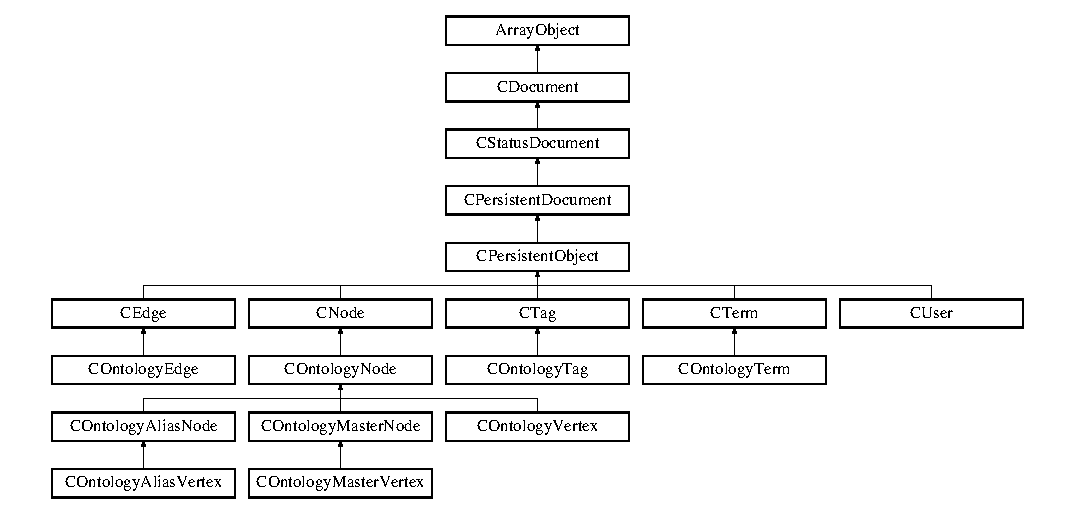
\includegraphics[height=6.461539cm]{class_c_persistent_object}
\end{center}
\end{figure}
\subsection*{Public Member Functions}
\begin{DoxyCompactItemize}
\item 
\hyperlink{class_c_persistent_object_a63f0a77d9664202a629f75be0a896659}{\-\_\-\-\_\-to\-String} ()
\item 
\hyperlink{class_c_persistent_object_abc705190184236693b30c15d7bc30b82}{G\-I\-D} (\$the\-Value=N\-U\-L\-L, \$get\-Old=F\-A\-L\-S\-E)
\item 
\hyperlink{class_c_persistent_object_a8ddd4477818aaff75a509b265dda77f1}{C\-Lass\-Name} (\$the\-Value=N\-U\-L\-L, \$get\-Old=F\-A\-L\-S\-E)
\end{DoxyCompactItemize}
\subsection*{Static Public Member Functions}
\begin{DoxyCompactItemize}
\item 
static \hyperlink{class_c_persistent_object_a5a5402ef394104148cfc580a6799ac2b}{New\-Object} (\hyperlink{class_c_connection}{C\-Connection} \$the\-Connection, \$the\-Identifier, \$do\-Throw=F\-A\-L\-S\-E)
\item 
static \hyperlink{class_c_persistent_object_a714b50e717e343bbc2e48861a30d624b}{Document\-Object} (\$the\-Document)
\item 
static \hyperlink{class_c_persistent_object_ace9f531fd290f67d5ef0398b5233d558}{\-\_\-id} (\$the\-Identifier=N\-U\-L\-L, \hyperlink{class_c_connection}{C\-Connection} \$the\-Connection=N\-U\-L\-L)
\end{DoxyCompactItemize}
\subsection*{Protected Member Functions}
\begin{DoxyCompactItemize}
\item 
\hyperlink{class_c_persistent_object_a34a9e2d5a39a5b8fb3ce00cf77c6a9d6}{\-\_\-index} (\hyperlink{class_c_connection}{C\-Connection} \$the\-Connection, \$the\-Modifiers)
\item 
\hyperlink{class_c_persistent_object_a01007da813afb05a7dce955501d5003c}{\-\_\-\-Preset} (\&\$the\-Offset, \&\$the\-Value)
\item 
\hyperlink{class_c_persistent_object_ae62466987d80bda95af79a3b9ffe65f3}{\-\_\-\-Preunset} (\&\$the\-Offset)
\item 
\hyperlink{class_c_persistent_object_a64945a54027c2940a4b1b6074c342bd3}{\-\_\-\-Precommit\-Validate} (\&\$the\-Connection, \&\$the\-Modifiers)
\item 
\hyperlink{class_c_persistent_object_a91707b0f40e344abbe3f7471d5e6a082}{\-\_\-\-Precommit\-Related} (\&\$the\-Connection, \&\$the\-Modifiers)
\item 
\hyperlink{class_c_persistent_object_a02d8bd3a63da4aca56af561cf18d32a4}{\-\_\-\-Precommit\-Identify} (\&\$the\-Connection, \&\$the\-Modifiers)
\item 
\hyperlink{class_c_persistent_object_ae5f9319ab169499181ae8db82b2fc0e7}{\-\_\-\-Reference\-In\-Object} (\hyperlink{class_c_container}{C\-Container} \$the\-Container, \$the\-Operation, \$the\-Reference, \$the\-Offset, \$the\-Count)
\item 
\hyperlink{class_c_persistent_object_aaddbaf409e7cab172ce6a92631d9ae45}{\-\_\-\-Assert\-Class} (\&\$the\-Value, \$the\-Base\-Class, \$the\-Derived\-Class=N\-U\-L\-L, \$do\-Throw=F\-A\-L\-S\-E)
\end{DoxyCompactItemize}
\subsection*{Additional Inherited Members}


\subsection{Member Function Documentation}
\hypertarget{class_c_persistent_object_a63f0a77d9664202a629f75be0a896659}{\index{C\-Persistent\-Object@{C\-Persistent\-Object}!\-\_\-\-\_\-to\-String@{\-\_\-\-\_\-to\-String}}
\index{\-\_\-\-\_\-to\-String@{\-\_\-\-\_\-to\-String}!CPersistentObject@{C\-Persistent\-Object}}
\subsubsection[{\-\_\-\-\_\-to\-String}]{\setlength{\rightskip}{0pt plus 5cm}C\-Persistent\-Object\-::\-\_\-\-\_\-to\-String (
\begin{DoxyParamCaption}
{}
\end{DoxyParamCaption}
)}}\label{class_c_persistent_object_a63f0a77d9664202a629f75be0a896659}
\subparagraph*{Return object name}

This method should return the current object's name which should represent the unique identifier of the object.

By default we return the value of the \hyperlink{}{k\-T\-A\-G\-\_\-\-G\-I\-D} offset, if this offset is missing, the method will return {\ttfamily N\-U\-L\-L}, which will result in a fatal error. This behaviour is intentional, since in this case the returned value is not correct and because this method cannot throw exceptions.

public \begin{DoxyReturn}{Returns}
string The connection name. 
\end{DoxyReturn}
\hypertarget{class_c_persistent_object_aaddbaf409e7cab172ce6a92631d9ae45}{\index{C\-Persistent\-Object@{C\-Persistent\-Object}!\-\_\-\-Assert\-Class@{\-\_\-\-Assert\-Class}}
\index{\-\_\-\-Assert\-Class@{\-\_\-\-Assert\-Class}!CPersistentObject@{C\-Persistent\-Object}}
\subsubsection[{\-\_\-\-Assert\-Class}]{\setlength{\rightskip}{0pt plus 5cm}C\-Persistent\-Object\-::\-\_\-\-Assert\-Class (
\begin{DoxyParamCaption}
\item[{\&}]{\$the\-Value, }
\item[{}]{\$the\-Base\-Class, }
\item[{}]{\$the\-Derived\-Class = {\ttfamily NULL}, }
\item[{}]{\$do\-Throw = {\ttfamily FALSE}}
\end{DoxyParamCaption}
)\hspace{0.3cm}{\ttfamily [protected]}}}\label{class_c_persistent_object_aaddbaf409e7cab172ce6a92631d9ae45}
\subparagraph*{Ensure the provided object is of the correct class}

This method can be used to check whether the provided value is of the correct class. the method will first check if the value corresponds to a base class, {\ttfamily \$the\-Base\-Class}, it will then check if the object is an instance of a derived class, {\ttfamily \$the\-Derived\-Class}.

If the value is not an object of the base class, the method will return {\ttfamily N\-U\-L\-L}, if the object is an instance of both the base and derived classes, the method will return {\ttfamily T\-R\-U\-E}; if the object is not an instance of the derived class\-: if the second parameter, {\ttfamily \$do\-Throw}, is {\ttfamily T\-R\-U\-E}, the method will raise an exception, if not, it will return {\ttfamily F\-A\-L\-S\-E}.

If you omit the derived class, the test will return {\ttfamily T\-R\-U\-E}, if the value is an instance of the base class.


\begin{DoxyParams}[1]{Parameters}
reference & {\em \$the\-Value} & Value to assert. \\
\hline
string & {\em \$the\-Base\-Class} & Base class to test. \\
\hline
string & {\em \$the\-Derived\-Class} & Derived class to test. \\
\hline
boolean & {\em \$do\-Throw} & If {\ttfamily T\-R\-U\-E} raise exception.\\
\hline
\end{DoxyParams}
protected \begin{DoxyReturn}{Returns}
mixed {\ttfamily T\-R\-U\-E} correct object,; {\ttfamily N\-U\-L\-L} bot an object; {\ttfamily F\-A\-L\-S\-E} not an object.
\end{DoxyReturn}

\begin{DoxyExceptions}{Exceptions}
{\em Exception} & \\
\hline
\end{DoxyExceptions}
\hypertarget{class_c_persistent_object_ace9f531fd290f67d5ef0398b5233d558}{\index{C\-Persistent\-Object@{C\-Persistent\-Object}!\-\_\-id@{\-\_\-id}}
\index{\-\_\-id@{\-\_\-id}!CPersistentObject@{C\-Persistent\-Object}}
\subsubsection[{\-\_\-id}]{\setlength{\rightskip}{0pt plus 5cm}static C\-Persistent\-Object\-::\-\_\-id (
\begin{DoxyParamCaption}
\item[{}]{\$the\-Identifier = {\ttfamily NULL}, }
\item[{{\bf C\-Connection}}]{\$the\-Connection = {\ttfamily NULL}}
\end{DoxyParamCaption}
)\hspace{0.3cm}{\ttfamily [static]}}}\label{class_c_persistent_object_ace9f531fd290f67d5ef0398b5233d558}
\subparagraph*{Generate the object's native unique identifier}

This method is used to generate the object's {\itshape native unique identifier}, \hyperlink{}{k\-T\-A\-G\-\_\-\-N\-I\-D}, from the string representing the object's {\itshape global unique identifier}, \hyperlink{}{k\-T\-A\-G\-\_\-\-G\-I\-D}.

The first parameter of the method is a string, the second parameter can be a server or database which can be resolved into a container, or the container itself. This parameter can be used to process the first one\-: since the resulting value must be stored in a container, it should be the duty of the container itself to convert, for instance binary strings, to a suitable value.

If the method receives {\ttfamily N\-U\-L\-L} in the first parameter, this means that the object does not use the global identifier and it is the duty of the container to set the object's primary key, such as with autonumbers in S\-Q\-L or missing {\ttfamily \-\_\-id} in Mongo. In that case this method should not be called, see the \hyperlink{class_c_persistent_document_a23cfbb5ebf75e008622ab9e723472c70}{\-\_\-\-Precommit()} method to see where it is used.

In this class we do not process the identifier, so we simply return it.


\begin{DoxyParams}[1]{Parameters}
string & {\em \$the\-Identifier} & Global unique identifier. \\
\hline
\hyperlink{class_c_connection}{C\-Connection} & {\em \$the\-Connection} & Server, database or container.\\
\hline
\end{DoxyParams}
\begin{DoxyReturn}{Returns}
mixed The object's native unique identifier. 
\end{DoxyReturn}
\hypertarget{class_c_persistent_object_a34a9e2d5a39a5b8fb3ce00cf77c6a9d6}{\index{C\-Persistent\-Object@{C\-Persistent\-Object}!\-\_\-index@{\-\_\-index}}
\index{\-\_\-index@{\-\_\-index}!CPersistentObject@{C\-Persistent\-Object}}
\subsubsection[{\-\_\-index}]{\setlength{\rightskip}{0pt plus 5cm}C\-Persistent\-Object\-::\-\_\-index (
\begin{DoxyParamCaption}
\item[{{\bf C\-Connection}}]{\$the\-Connection, }
\item[{}]{\$the\-Modifiers}
\end{DoxyParamCaption}
)\hspace{0.3cm}{\ttfamily [protected]}}}\label{class_c_persistent_object_a34a9e2d5a39a5b8fb3ce00cf77c6a9d6}
\subparagraph*{Return the object's global unique identifier}

This method should return the object's global unique identifier, this value is represented by a string which is generally extracted from selected attributes of the object and constitutes the unique key of the object.

This string is stored in the \hyperlink{}{k\-T\-A\-G\-\_\-\-G\-I\-D} offset of the object and it is processed by the static \hyperlink{class_c_persistent_object_ace9f531fd290f67d5ef0398b5233d558}{\-\_\-id()} method to generate the object's native unique identifier, which is the native object's primary key stored in the \hyperlink{}{k\-T\-A\-G\-\_\-\-N\-I\-D} offset.

This method is called by the \hyperlink{class_c_persistent_document_a23cfbb5ebf75e008622ab9e723472c70}{\-\_\-\-Precommit()} method, to fill the \hyperlink{}{k\-T\-A\-G\-\_\-\-G\-I\-D} offset and the resulting value is fed to the \hyperlink{class_c_persistent_object_ace9f531fd290f67d5ef0398b5233d558}{\-\_\-id()} method to obtain the value that will be stored in the \hyperlink{}{k\-T\-A\-G\-\_\-\-N\-I\-D} offset. The inherited \hyperlink{}{Precommit()} method asserts whether the object \hyperlink{class_c_status_document_a954dee06e219e0a0f2e7fa6edac56e28}{\-\_\-\-Is\-Inited()}, before calling the local \hyperlink{class_c_persistent_document_a23cfbb5ebf75e008622ab9e723472c70}{\-\_\-\-Precommit()} method, this to ensure that this method can safely use the object's attributes to generate the identifier. If you intend to use this method in other places, you should check if the object is initialised.

If the object does not feature or use the global identifier, this method should return {\ttfamily N\-U\-L\-L}, this will be an indication that the native identifier is filled in another place, or that the identifier is filled by the container.

The method accepts the same parameters as the \hyperlink{}{Precommit()} method which passes them to this one. The first one should resolve into the container in which the object will be saved, this parameter can be useful when committing embedded objects which reside in different containers. The second parameter represents the operation options which can be useful to determine whether the object is being inserted, replaced or updated.

In this class we do not have attributes that can be used to generate an identifier, so we let the container set the identifier, and return {\ttfamily N\-U\-L\-L}.


\begin{DoxyParams}[1]{Parameters}
\hyperlink{class_c_connection}{C\-Connection} & {\em \$the\-Connection} & Server, database or container. \\
\hline
bitfield & {\em \$the\-Modifiers} & Commit options.\\
\hline
\end{DoxyParams}
protected \begin{DoxyReturn}{Returns}
string$|$\-N\-U\-L\-L The object's global unique identifier. 
\end{DoxyReturn}
\hypertarget{class_c_persistent_object_a02d8bd3a63da4aca56af561cf18d32a4}{\index{C\-Persistent\-Object@{C\-Persistent\-Object}!\-\_\-\-Precommit\-Identify@{\-\_\-\-Precommit\-Identify}}
\index{\-\_\-\-Precommit\-Identify@{\-\_\-\-Precommit\-Identify}!CPersistentObject@{C\-Persistent\-Object}}
\subsubsection[{\-\_\-\-Precommit\-Identify}]{\setlength{\rightskip}{0pt plus 5cm}C\-Persistent\-Object\-::\-\_\-\-Precommit\-Identify (
\begin{DoxyParamCaption}
\item[{\&}]{\$the\-Connection, }
\item[{\&}]{\$the\-Modifiers}
\end{DoxyParamCaption}
)\hspace{0.3cm}{\ttfamily [protected]}}}\label{class_c_persistent_object_a02d8bd3a63da4aca56af561cf18d32a4}
\subparagraph*{Determine the identifiers before committing}

In this class this method is called only if the operation involves inserting or replacing.

If the \hyperlink{}{k\-T\-A\-G\-\_\-\-G\-I\-D} offset is missing, we call the \hyperlink{class_c_persistent_object_a34a9e2d5a39a5b8fb3ce00cf77c6a9d6}{\-\_\-index()} method\-: if the result of that method is not {\ttfamily N\-U\-L\-L}, we use it to set the \hyperlink{}{k\-T\-A\-G\-\_\-\-G\-I\-D} offset value, this only if the operation involves inserting or replacing.

If the \hyperlink{}{k\-T\-A\-G\-\_\-\-N\-I\-D} offset is missing, we check if the \hyperlink{}{k\-T\-A\-G\-\_\-\-G\-I\-D} offset was set\-: in that case we use its value to feed the \hyperlink{class_c_persistent_object_ace9f531fd290f67d5ef0398b5233d558}{\-\_\-id()} method and the result is set in the \hyperlink{}{k\-T\-A\-G\-\_\-\-N\-I\-D} offset.

This workflow implies that only if the \hyperlink{class_c_persistent_object_a34a9e2d5a39a5b8fb3ce00cf77c6a9d6}{\-\_\-index()} method returns a non {\ttfamily N\-U\-L\-L} value, the \hyperlink{}{k\-T\-A\-G\-\_\-\-G\-I\-D} offset will be set in this method, and that if the \hyperlink{}{k\-T\-A\-G\-\_\-\-G\-I\-D} offset is missing the native identifier will not be touched.

Note that this is the only place in which the \hyperlink{class_c_persistent_object_a34a9e2d5a39a5b8fb3ce00cf77c6a9d6}{\-\_\-index()} method is called.


\begin{DoxyParams}[1]{Parameters}
reference & {\em \&\$the\-Connection} & Server, database or container. \\
\hline
reference & {\em \&\$the\-Modifiers} & Commit options.\\
\hline
\end{DoxyParams}
protected \begin{DoxyReturn}{Returns}
mixed
\end{DoxyReturn}
\hyperlink{class_c_persistent_object_ace9f531fd290f67d5ef0398b5233d558}{\-\_\-id()}  \hyperlink{class_c_persistent_object_a34a9e2d5a39a5b8fb3ce00cf77c6a9d6}{\-\_\-index()}  \hyperlink{class_c_persistent_document_a4dbe287aa3b46bdc0a1157e001078589}{Resolve\-Container()}

\begin{DoxySeeAlso}{See Also}
k\-T\-A\-G\-\_\-\-G\-I\-D k\-T\-A\-G\-\_\-\-N\-I\-D 

k\-F\-L\-A\-G\-\_\-\-P\-E\-R\-S\-I\-S\-T\-\_\-\-I\-N\-S\-E\-R\-T k\-F\-L\-A\-G\-\_\-\-P\-E\-R\-S\-I\-S\-T\-\_\-\-R\-E\-P\-L\-A\-C\-E 
\end{DoxySeeAlso}
\hypertarget{class_c_persistent_object_a91707b0f40e344abbe3f7471d5e6a082}{\index{C\-Persistent\-Object@{C\-Persistent\-Object}!\-\_\-\-Precommit\-Related@{\-\_\-\-Precommit\-Related}}
\index{\-\_\-\-Precommit\-Related@{\-\_\-\-Precommit\-Related}!CPersistentObject@{C\-Persistent\-Object}}
\subsubsection[{\-\_\-\-Precommit\-Related}]{\setlength{\rightskip}{0pt plus 5cm}C\-Persistent\-Object\-::\-\_\-\-Precommit\-Related (
\begin{DoxyParamCaption}
\item[{\&}]{\$the\-Connection, }
\item[{\&}]{\$the\-Modifiers}
\end{DoxyParamCaption}
)\hspace{0.3cm}{\ttfamily [protected]}}}\label{class_c_persistent_object_a91707b0f40e344abbe3f7471d5e6a082}
\subparagraph*{Handle embedded or related objects before committing}

In this class we have no related objects, but we use this method to set default values, such as the class name in \hyperlink{}{k\-T\-A\-G\-\_\-\-C\-L\-A\-S\-S} when inserting, replacing or updating.


\begin{DoxyParams}[1]{Parameters}
reference & {\em \&\$the\-Connection} & Server, database or container. \\
\hline
reference & {\em \&\$the\-Modifiers} & Commit options.\\
\hline
\end{DoxyParams}
protected \begin{DoxyReturn}{Returns}
mixed
\end{DoxyReturn}
\begin{DoxySeeAlso}{See Also}
k\-T\-A\-G\-\_\-\-C\-L\-A\-S\-S 

k\-F\-L\-A\-G\-\_\-\-P\-E\-R\-S\-I\-S\-T\-\_\-\-I\-N\-S\-E\-R\-T k\-F\-L\-A\-G\-\_\-\-P\-E\-R\-S\-I\-S\-T\-\_\-\-R\-E\-P\-L\-A\-C\-E k\-F\-L\-A\-G\-\_\-\-P\-E\-R\-S\-I\-S\-T\-\_\-\-U\-P\-D\-A\-T\-E 
\end{DoxySeeAlso}
\hypertarget{class_c_persistent_object_a64945a54027c2940a4b1b6074c342bd3}{\index{C\-Persistent\-Object@{C\-Persistent\-Object}!\-\_\-\-Precommit\-Validate@{\-\_\-\-Precommit\-Validate}}
\index{\-\_\-\-Precommit\-Validate@{\-\_\-\-Precommit\-Validate}!CPersistentObject@{C\-Persistent\-Object}}
\subsubsection[{\-\_\-\-Precommit\-Validate}]{\setlength{\rightskip}{0pt plus 5cm}C\-Persistent\-Object\-::\-\_\-\-Precommit\-Validate (
\begin{DoxyParamCaption}
\item[{\&}]{\$the\-Connection, }
\item[{\&}]{\$the\-Modifiers}
\end{DoxyParamCaption}
)\hspace{0.3cm}{\ttfamily [protected]}}}\label{class_c_persistent_object_a64945a54027c2940a4b1b6074c342bd3}
\subparagraph*{Validate the object before committing}

In this class we check if the current object has its native identifier, \hyperlink{}{k\-T\-A\-G\-\_\-\-N\-I\-D}, if the operation involves updating.


\begin{DoxyParams}[1]{Parameters}
reference & {\em \&\$the\-Connection} & Server, database or container. \\
\hline
reference & {\em \&\$the\-Modifiers} & Commit options.\\
\hline
\end{DoxyParams}
protected \begin{DoxyReturn}{Returns}
mixed
\end{DoxyReturn}

\begin{DoxyExceptions}{Exceptions}
{\em Exception} & \\
\hline
\end{DoxyExceptions}
\begin{DoxySeeAlso}{See Also}
k\-F\-L\-A\-G\-\_\-\-P\-E\-R\-S\-I\-S\-T\-\_\-\-M\-A\-S\-K k\-F\-L\-A\-G\-\_\-\-P\-E\-R\-S\-I\-S\-T\-\_\-\-U\-P\-D\-A\-T\-E k\-T\-A\-G\-\_\-\-N\-I\-D 
\end{DoxySeeAlso}
\hypertarget{class_c_persistent_object_a01007da813afb05a7dce955501d5003c}{\index{C\-Persistent\-Object@{C\-Persistent\-Object}!\-\_\-\-Preset@{\-\_\-\-Preset}}
\index{\-\_\-\-Preset@{\-\_\-\-Preset}!CPersistentObject@{C\-Persistent\-Object}}
\subsubsection[{\-\_\-\-Preset}]{\setlength{\rightskip}{0pt plus 5cm}C\-Persistent\-Object\-::\-\_\-\-Preset (
\begin{DoxyParamCaption}
\item[{\&}]{\$the\-Offset, }
\item[{\&}]{\$the\-Value}
\end{DoxyParamCaption}
)\hspace{0.3cm}{\ttfamily [protected]}}}\label{class_c_persistent_object_a01007da813afb05a7dce955501d5003c}
\subparagraph*{Handle offset before setting it}

In this class we prevent the modification of offsets that concur in the generation of the object's identifier if the object has its \hyperlink{class_c_status_document_ab7d96fd4588cf7d5432fc65a1d1fb076}{\-\_\-\-Is\-Committed()} status set. This is because referenced objects must not change identifier.


\begin{DoxyParams}[1]{Parameters}
reference & {\em \&\$the\-Offset} & Offset. \\
\hline
reference & {\em \&\$the\-Value} & Value to set at offset.\\
\hline
\end{DoxyParams}
protected


\begin{DoxyExceptions}{Exceptions}
{\em Exception} & \hyperlink{class_c_status_document_ab7d96fd4588cf7d5432fc65a1d1fb076}{\-\_\-\-Is\-Committed()}\\
\hline
\end{DoxyExceptions}
\begin{DoxySeeAlso}{See Also}
k\-T\-A\-G\-\_\-\-N\-I\-D k\-T\-A\-G\-\_\-\-G\-I\-D 
\end{DoxySeeAlso}
\hypertarget{class_c_persistent_object_ae62466987d80bda95af79a3b9ffe65f3}{\index{C\-Persistent\-Object@{C\-Persistent\-Object}!\-\_\-\-Preunset@{\-\_\-\-Preunset}}
\index{\-\_\-\-Preunset@{\-\_\-\-Preunset}!CPersistentObject@{C\-Persistent\-Object}}
\subsubsection[{\-\_\-\-Preunset}]{\setlength{\rightskip}{0pt plus 5cm}C\-Persistent\-Object\-::\-\_\-\-Preunset (
\begin{DoxyParamCaption}
\item[{\&}]{\$the\-Offset}
\end{DoxyParamCaption}
)\hspace{0.3cm}{\ttfamily [protected]}}}\label{class_c_persistent_object_ae62466987d80bda95af79a3b9ffe65f3}
\subparagraph*{Handle offset before unsetting it}

In this class we prevent the modification of offsets that concur in the generation of the object's identifier if the object has its \hyperlink{class_c_status_document_ab7d96fd4588cf7d5432fc65a1d1fb076}{\-\_\-\-Is\-Committed()} status set. This is because referenced objects must not change identifier.


\begin{DoxyParams}[1]{Parameters}
reference & {\em \&\$the\-Offset} & Offset.\\
\hline
\end{DoxyParams}
protected


\begin{DoxyExceptions}{Exceptions}
{\em Exception} & \hyperlink{class_c_status_document_ab7d96fd4588cf7d5432fc65a1d1fb076}{\-\_\-\-Is\-Committed()}\\
\hline
\end{DoxyExceptions}
\begin{DoxySeeAlso}{See Also}
k\-T\-A\-G\-\_\-\-N\-I\-D k\-T\-A\-G\-\_\-\-G\-I\-D 
\end{DoxySeeAlso}
\hypertarget{class_c_persistent_object_ae5f9319ab169499181ae8db82b2fc0e7}{\index{C\-Persistent\-Object@{C\-Persistent\-Object}!\-\_\-\-Reference\-In\-Object@{\-\_\-\-Reference\-In\-Object}}
\index{\-\_\-\-Reference\-In\-Object@{\-\_\-\-Reference\-In\-Object}!CPersistentObject@{C\-Persistent\-Object}}
\subsubsection[{\-\_\-\-Reference\-In\-Object}]{\setlength{\rightskip}{0pt plus 5cm}C\-Persistent\-Object\-::\-\_\-\-Reference\-In\-Object (
\begin{DoxyParamCaption}
\item[{{\bf C\-Container}}]{\$the\-Container, }
\item[{}]{\$the\-Operation, }
\item[{}]{\$the\-Reference, }
\item[{}]{\$the\-Offset, }
\item[{}]{\$the\-Count}
\end{DoxyParamCaption}
)\hspace{0.3cm}{\ttfamily [protected]}}}\label{class_c_persistent_object_ae5f9319ab169499181ae8db82b2fc0e7}
\subparagraph*{add, increment, remove or decrement current object's reference}

This method can be used to reference the current object in another object by either incrementing/decrementing a counter in the target object, or adding/removing a reference of the current object from the target object.

The method accepts the following parameters\-:


\begin{DoxyItemize}
\item {\ttfamily \$the\-Container}\-: Container in which the target object is stored. 
\item {\ttfamily \$the\-Operation}\-: This value determines what kind of operation to perform\-: 
\begin{DoxyItemize}
\item {\ttfamily 0x2}\-: {\itshape Keep reference count}. This means that the {\ttfamily \$the\-Offset} attribute will be an integer representing the number of times the target object was referenced. 
\item {\ttfamily 0x3}\-: {\itshape Keep references list}. This means that the {\ttfamily \$the\-Offset} attribute will be a list of object identifiers representing the objects that reference the target object. 
\item {\itshape other}\-: {\itshape Ignore}. Any other value will disable this method. 
\end{DoxyItemize}
\item {\ttfamily \$the\-Reference}\-: This value represents the native identifier of the object that receives the reference. 
\item {\ttfamily \$the\-Count}\-: This value represents the increment/decrement value, or a value whose sign will be used to determine whether to add or remove references from the list\-: a negative value means remove, a positive value means add; if the value is {\ttfamily 0}, the method will do nothing. 
\end{DoxyItemize}

The method will return {\ttfamily T\-R\-U\-E} if the operation affected at least one object, {\ttfamily F\-A\-L\-S\-E} if not, {\ttfamily N\-U\-L\-L} if the provided increment is {\ttfamily 0} and raise an exception if the operation failed.

{\itshape Note that this method does not check if the object is committed, that must have been done by the caller. This method is called in general after inserting the object and before setting the committed status}.


\begin{DoxyParams}[1]{Parameters}
\hyperlink{class_c_container}{C\-Container} & {\em \$the\-Container} & Server, database or container. \\
\hline
byte & {\em \$the\-Operation} & Operation code. \\
\hline
mixed & {\em \$the\-Reference} & Target object reference. \\
\hline
string & {\em \$the\-Offset} & Offset to update. \\
\hline
integer & {\em \$the\-Count} & Increment amount.\\
\hline
\end{DoxyParams}
protected \begin{DoxyReturn}{Returns}
mixed {\ttfamily T\-R\-U\-E} operation affected at least one object. 
\end{DoxyReturn}
\hypertarget{class_c_persistent_object_a8ddd4477818aaff75a509b265dda77f1}{\index{C\-Persistent\-Object@{C\-Persistent\-Object}!C\-Lass\-Name@{C\-Lass\-Name}}
\index{C\-Lass\-Name@{C\-Lass\-Name}!CPersistentObject@{C\-Persistent\-Object}}
\subsubsection[{C\-Lass\-Name}]{\setlength{\rightskip}{0pt plus 5cm}C\-Persistent\-Object\-::\-C\-Lass\-Name (
\begin{DoxyParamCaption}
\item[{}]{\$the\-Value = {\ttfamily NULL}, }
\item[{}]{\$get\-Old = {\ttfamily FALSE}}
\end{DoxyParamCaption}
)}}\label{class_c_persistent_object_a8ddd4477818aaff75a509b265dda77f1}
\subparagraph*{Manage class identifier}

The {\itshape class name}, \hyperlink{}{k\-T\-A\-G\-\_\-\-C\-L\-A\-S\-S}, holds a string which is the class name of the object that first stored the object in the container. This value will be used by the static \hyperlink{class_c_persistent_object_a5a5402ef394104148cfc580a6799ac2b}{New\-Object()} method to restore the object from the container.

The method accepts a parameter which represents either the name or the requested operation, depending on its value\-:


\begin{DoxyItemize}
\item {\ttfamily N\-U\-L\-L}\-: Return the current value. 
\item {\ttfamily F\-A\-L\-S\-E}\-: Delete the current value. 
\item {\itshape other}\-: Set the value with the provided parameter. 
\end{DoxyItemize}

The second parameter is a boolean which if {\ttfamily T\-R\-U\-E} will return the {\itshape old} value when replacing an existing value; if {\ttfamily F\-A\-L\-S\-E}, it will return the currently set value.

Note that, while this method allows the creation, modification and deletion of this property, the hosting object may prevent some of these actions, by default this attribute is locked when the object has the \hyperlink{class_c_status_document_ab7d96fd4588cf7d5432fc65a1d1fb076}{\-\_\-\-Is\-Committed()} status.

In general you should not set this value directly, since it will be set programmatically.


\begin{DoxyParams}[1]{Parameters}
mixed & {\em \$the\-Value} & Class name or operation. \\
\hline
boolean & {\em \$get\-Old} & {\ttfamily T\-R\-U\-E} get old value.\\
\hline
\end{DoxyParams}
public \begin{DoxyReturn}{Returns}
string {\itshape New}, {\itshape old} value or {\ttfamily N\-U\-L\-L}.
\end{DoxyReturn}
Manage\-Offset()

\begin{DoxySeeAlso}{See Also}
k\-T\-A\-G\-\_\-\-C\-L\-A\-S\-S 
\end{DoxySeeAlso}
\hypertarget{class_c_persistent_object_a714b50e717e343bbc2e48861a30d624b}{\index{C\-Persistent\-Object@{C\-Persistent\-Object}!Document\-Object@{Document\-Object}}
\index{Document\-Object@{Document\-Object}!CPersistentObject@{C\-Persistent\-Object}}
\subsubsection[{Document\-Object}]{\setlength{\rightskip}{0pt plus 5cm}static C\-Persistent\-Object\-::\-Document\-Object (
\begin{DoxyParamCaption}
\item[{}]{\$the\-Document}
\end{DoxyParamCaption}
)\hspace{0.3cm}{\ttfamily [static]}}}\label{class_c_persistent_object_a714b50e717e343bbc2e48861a30d624b}
\subparagraph*{Instantiate an object from a document}

This method can be used to instantiate an object from an array. The method will attempt to locate the class name, \hyperlink{}{k\-T\-A\-G\-\_\-\-C\-L\-A\-S\-S}, if found, it will return an object of that class, if not, it will return the unchanged received document.

If the class name was found, the resulting object will have its \hyperlink{class_c_status_document_ab7d96fd4588cf7d5432fc65a1d1fb076}{\-\_\-\-Is\-Committed()} status set, so provide only data received from database queries.

The method accepts arrays and Array\-Objects, any other type will raise an exception.


\begin{DoxyParams}[1]{Parameters}
mixed & {\em \$the\-Document} & Persistent object data.\\
\hline
\end{DoxyParams}
\begin{DoxyReturn}{Returns}
mixed The document or an object. 
\end{DoxyReturn}
\hypertarget{class_c_persistent_object_abc705190184236693b30c15d7bc30b82}{\index{C\-Persistent\-Object@{C\-Persistent\-Object}!G\-I\-D@{G\-I\-D}}
\index{G\-I\-D@{G\-I\-D}!CPersistentObject@{C\-Persistent\-Object}}
\subsubsection[{G\-I\-D}]{\setlength{\rightskip}{0pt plus 5cm}C\-Persistent\-Object\-::\-G\-I\-D (
\begin{DoxyParamCaption}
\item[{}]{\$the\-Value = {\ttfamily NULL}, }
\item[{}]{\$get\-Old = {\ttfamily FALSE}}
\end{DoxyParamCaption}
)}}\label{class_c_persistent_object_abc705190184236693b30c15d7bc30b82}
\subparagraph*{Manage global unique identifier}

The {\itshape global unique identifier}, \hyperlink{}{k\-T\-A\-G\-\_\-\-G\-I\-D}, holds a string value which represents the object's unique identifier. This value is usually a computed string value extracted from a series of key properties of the object.

In general, the hashed value of this property becomes the object's native identifier, \hyperlink{class_c_persistent_document_ad9d15abc074aa3f779f214771b6123b0}{N\-I\-D()} and while the latter represents a native value, this property represents the global or public identifier of the object.

The method accepts a parameter which represents either the new value or the requested operation, depending on its type\-:


\begin{DoxyItemize}
\item {\ttfamily N\-U\-L\-L}\-: Return the current value. 
\item {\ttfamily F\-A\-L\-S\-E}\-: Delete the current value. 
\item {\itshape other}\-: Set the value with the provided parameter. 
\end{DoxyItemize}

The second parameter is a boolean which if {\ttfamily T\-R\-U\-E} will return the {\itshape old} value when replacing an existing value; if {\ttfamily F\-A\-L\-S\-E}, it will return the currently set value.

Note that, while this method allows the creation, modification and deletion of this property, the hosting object may prevent some of these actions, by default this attribute is locked when the object has the \hyperlink{class_c_status_document_ab7d96fd4588cf7d5432fc65a1d1fb076}{\-\_\-\-Is\-Committed()} status.


\begin{DoxyParams}[1]{Parameters}
mixed & {\em \$the\-Value} & Global identifier or operation. \\
\hline
boolean & {\em \$get\-Old} & {\ttfamily T\-R\-U\-E} get old value.\\
\hline
\end{DoxyParams}
public \begin{DoxyReturn}{Returns}
string {\itshape New}, {\itshape old} value or {\ttfamily N\-U\-L\-L}.
\end{DoxyReturn}
Manage\-Offset()

\begin{DoxySeeAlso}{See Also}
k\-T\-A\-G\-\_\-\-G\-I\-D 
\end{DoxySeeAlso}
\hypertarget{class_c_persistent_object_a5a5402ef394104148cfc580a6799ac2b}{\index{C\-Persistent\-Object@{C\-Persistent\-Object}!New\-Object@{New\-Object}}
\index{New\-Object@{New\-Object}!CPersistentObject@{C\-Persistent\-Object}}
\subsubsection[{New\-Object}]{\setlength{\rightskip}{0pt plus 5cm}static C\-Persistent\-Object\-::\-New\-Object (
\begin{DoxyParamCaption}
\item[{{\bf C\-Connection}}]{\$the\-Connection, }
\item[{}]{\$the\-Identifier, }
\item[{}]{\$do\-Throw = {\ttfamily FALSE}}
\end{DoxyParamCaption}
)\hspace{0.3cm}{\ttfamily [static]}}}\label{class_c_persistent_object_a5a5402ef394104148cfc580a6799ac2b}
\subparagraph*{Instantiate an object from a container}

We override this method to handle the \hyperlink{}{k\-T\-A\-G\-\_\-\-C\-L\-A\-S\-S} offset\-: if found in the retrieved object, it will be used to instantiate the correct class. If the offset is missing, the method will instantiate the calling class.

The method expects two parameters\-:


\begin{DoxyItemize}
\item {\ttfamily \$the\-Connection}\-: The container in which the object should be stored. This parameter should be a concrete instance of of \hyperlink{class_c_container}{C\-Container}, or a concrete instance of \hyperlink{class_c_server}{C\-Server} or \hyperlink{class_c_database}{C\-Database}, if the current class has implemented the container resolve interface with \hyperlink{class_c_persistent_document_a6092e640e36485873b70a79db464e0ff}{Default\-Database} and \hyperlink{class_c_persistent_document_ada019252d242b5a88a26b82a18e29ed6}{Default\-Container()}. 
\item {\ttfamily \$the\-Identifier}\-: The key of the object in the container, by default the \hyperlink{}{k\-T\-A\-G\-\_\-\-N\-I\-D} offset. 
\item {\ttfamily \$do\-Throw}\-: If {\ttfamily T\-R\-U\-E}, any failure to resolve the object will raise an exception. 
\end{DoxyItemize}

If the object could not be located, the method will return {\ttfamily N\-U\-L\-L}.


\begin{DoxyParams}[1]{Parameters}
\hyperlink{class_c_connection}{C\-Connection} & {\em \$the\-Connection} & Server, database or container. \\
\hline
mixed & {\em \$the\-Identifier} & Identifier. \\
\hline
boolean & {\em \$do\-Throw} & If {\ttfamily T\-R\-U\-E} raise an exception.\\
\hline
\end{DoxyParams}
\begin{DoxyReturn}{Returns}
mixed The retrieved object. 
\end{DoxyReturn}


The documentation for this class was generated from the following file\-:\begin{DoxyCompactItemize}
\item 
/\-Library/\-Web\-Server/\-Library/\-P\-H\-P\-Wrapper/classes/C\-Persistent\-Object.\-php\end{DoxyCompactItemize}

\hypertarget{class_c_portal_wrapper}{\section{C\-Portal\-Wrapper Class Reference}
\label{class_c_portal_wrapper}\index{C\-Portal\-Wrapper@{C\-Portal\-Wrapper}}
}
Inheritance diagram for C\-Portal\-Wrapper\-:\begin{figure}[H]
\begin{center}
\leavevmode
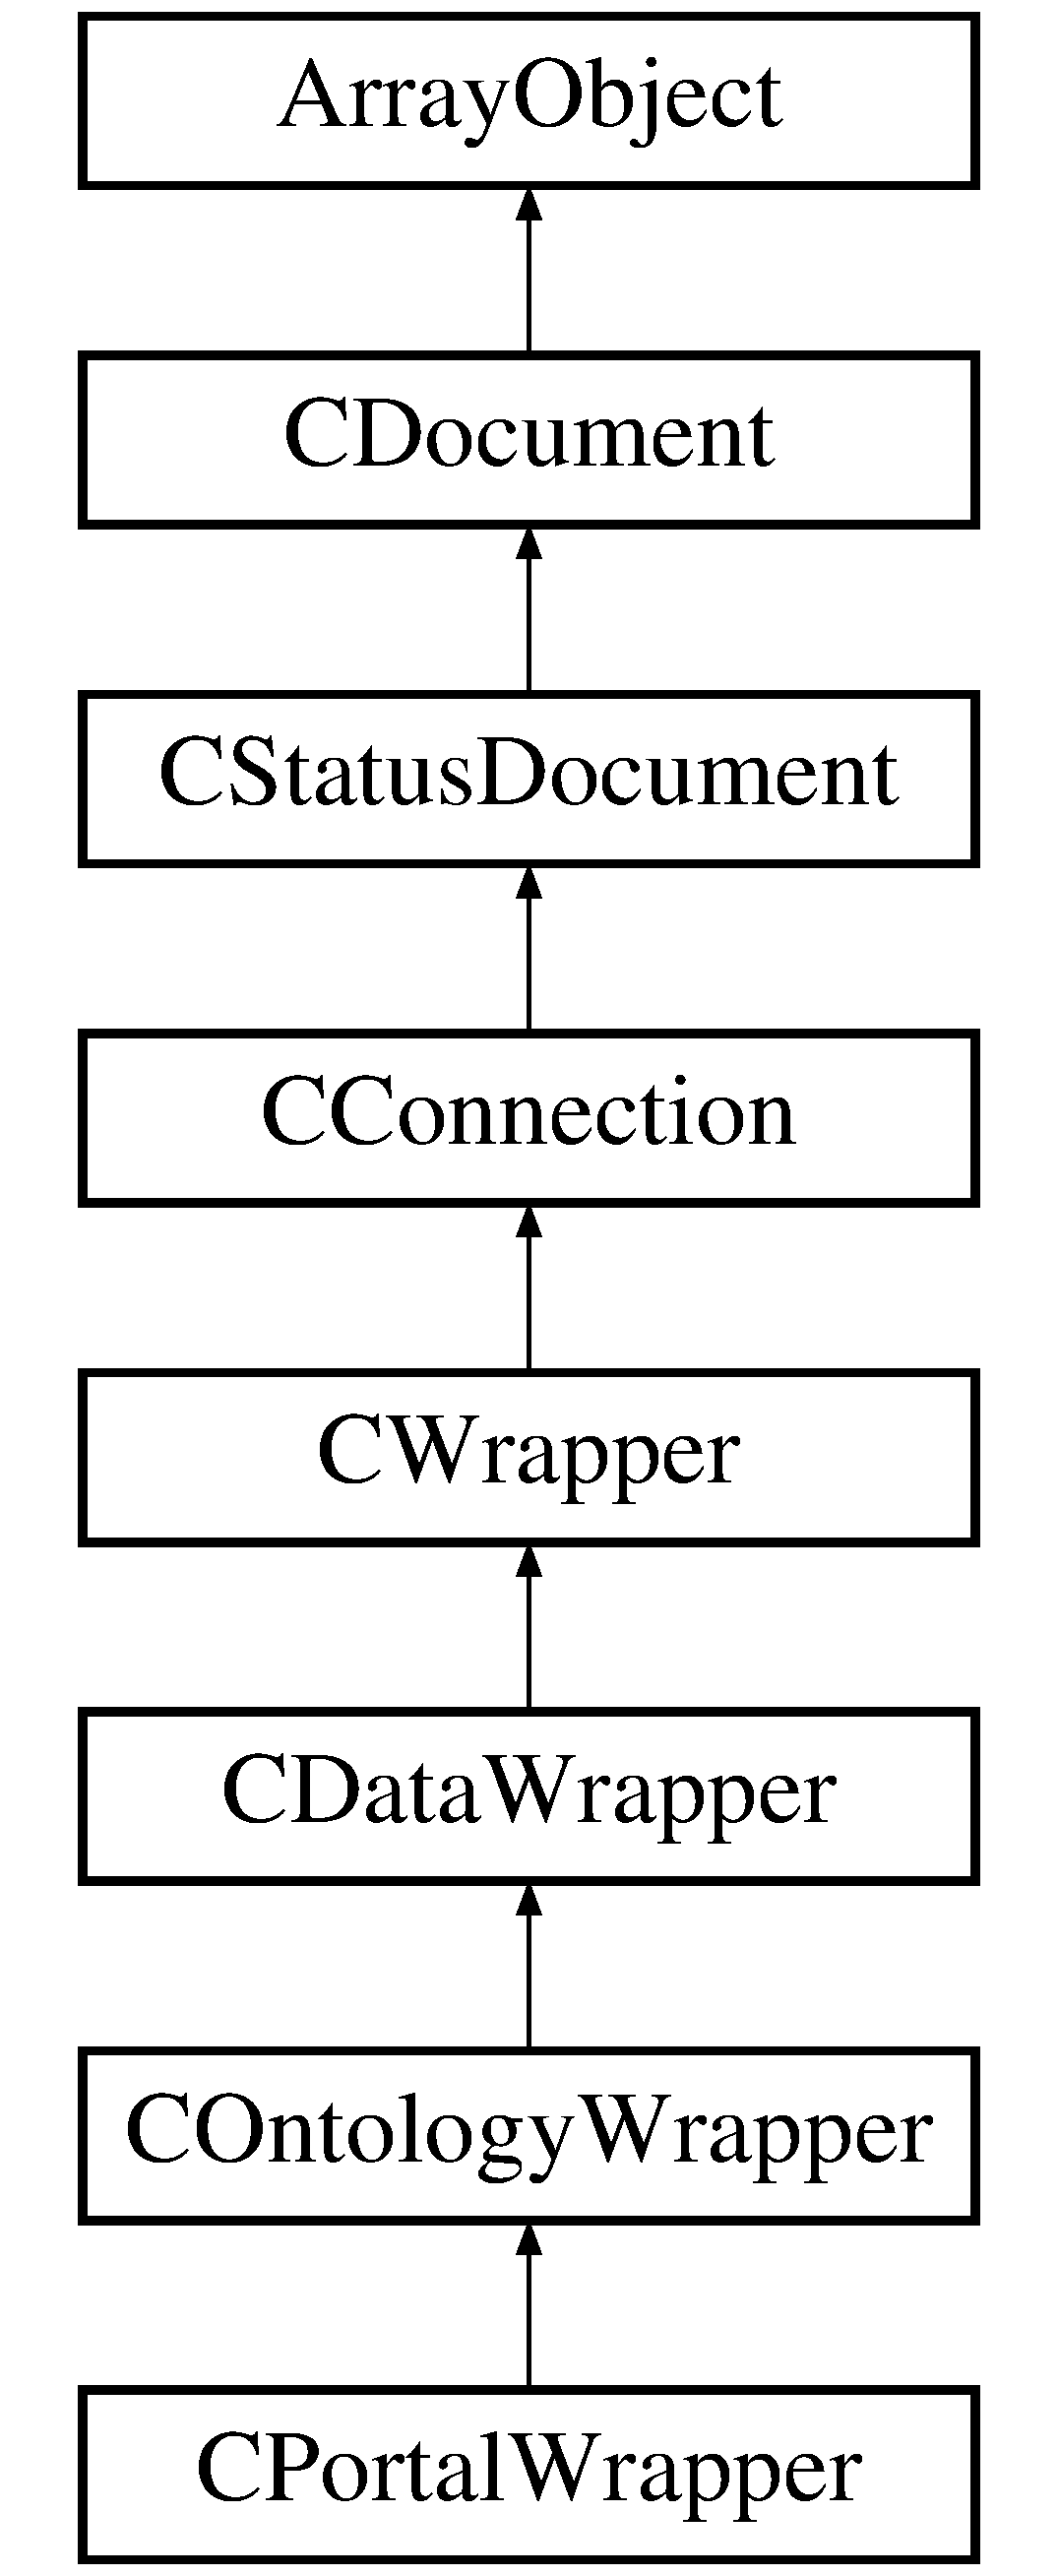
\includegraphics[height=8.000000cm]{class_c_portal_wrapper}
\end{center}
\end{figure}
\subsection*{Static Public Attributes}
\begin{DoxyCompactItemize}
\item 
\hypertarget{class_c_portal_wrapper_a958c92aeb9d0db3d7b67d3077da391f3}{static {\bfseries \$s\-Parameter\-List} = array( k\-A\-P\-I\-\_\-\-C\-R\-E\-D\-E\-N\-T\-I\-A\-L\-S )}\label{class_c_portal_wrapper_a958c92aeb9d0db3d7b67d3077da391f3}

\end{DoxyCompactItemize}
\subsection*{Protected Member Functions}
\begin{DoxyCompactItemize}
\item 
\hyperlink{class_c_portal_wrapper_a9082dde4409ea5d460735f5fe491d7d3}{\-\_\-\-Parse\-Request} ()
\item 
\hyperlink{class_c_portal_wrapper_ad6644c207927f83b3b41fefe894db393}{\-\_\-\-Format\-Request} ()
\item 
\hyperlink{class_c_portal_wrapper_a82b5b4d84bd970e44f451f095eeded9e}{\-\_\-\-Validate\-Request} ()
\item 
\hyperlink{class_c_portal_wrapper_ac8bfaffec1025ce29086a029cfad77bc}{\-\_\-\-Init\-Parameters} ()
\item 
\hyperlink{class_c_portal_wrapper_a03d714c9f08a5eeb3e70236ba8d71462}{\-\_\-\-Parse\-Operation} ()
\item 
\hyperlink{class_c_portal_wrapper_a92b44aafb5a9c21f6c3f0fcd51c907b8}{\-\_\-\-Parse\-Credentials} ()
\item 
\hyperlink{class_c_portal_wrapper_a0bf9f920e3b9c4e5b1db54a99a5e9185}{\-\_\-\-Format\-Credentials} ()
\item 
\hyperlink{class_c_portal_wrapper_a9d1a2d62ef4709f342221d97ed46b039}{\-\_\-\-Validate\-Operation} ()
\item 
\hyperlink{class_c_portal_wrapper_a906c6d7d2de1b9758c19c7a2e94a268d}{\-\_\-\-Validate\-Credentials} ()
\item 
\hyperlink{class_c_portal_wrapper_aaaa774d63578e176bd3f164736e832eb}{\-\_\-\-Validate\-New\-User} ()
\item 
\hyperlink{class_c_portal_wrapper_a35b88e5fd2364854c25bebdd43175392}{\-\_\-\-Handle\-Request} ()
\item 
\hyperlink{class_c_portal_wrapper_a3e1e82d3b794c7a154ce43d5b8b67bfd}{\-\_\-\-Handle\-\_\-\-List\-Op} (\&\$the\-List)
\item 
\hyperlink{class_c_portal_wrapper_a5209b3939911276e330c9bb3e1054001}{\-\_\-\-Handle\-\_\-\-Login} ()
\item 
\hyperlink{class_c_portal_wrapper_a0906c02f709cbdb701389aaebad5f2e4}{\-\_\-\-Handle\-\_\-\-New\-User} ()
\end{DoxyCompactItemize}
\subsection*{Additional Inherited Members}


\subsection{Member Function Documentation}
\hypertarget{class_c_portal_wrapper_a0bf9f920e3b9c4e5b1db54a99a5e9185}{\index{C\-Portal\-Wrapper@{C\-Portal\-Wrapper}!\-\_\-\-Format\-Credentials@{\-\_\-\-Format\-Credentials}}
\index{\-\_\-\-Format\-Credentials@{\-\_\-\-Format\-Credentials}!CPortalWrapper@{C\-Portal\-Wrapper}}
\subsubsection[{\-\_\-\-Format\-Credentials}]{\setlength{\rightskip}{0pt plus 5cm}C\-Portal\-Wrapper\-::\-\_\-\-Format\-Credentials (
\begin{DoxyParamCaption}
{}
\end{DoxyParamCaption}
)\hspace{0.3cm}{\ttfamily [protected]}}}\label{class_c_portal_wrapper_a0bf9f920e3b9c4e5b1db54a99a5e9185}
Format credentials parameters.

This method should format the provided credentials, in this class we do nothing.

protected

\begin{DoxySeeAlso}{See Also}
k\-A\-P\-I\-\_\-\-C\-R\-E\-D\-E\-N\-T\-I\-A\-L\-S 
\end{DoxySeeAlso}
\hypertarget{class_c_portal_wrapper_ad6644c207927f83b3b41fefe894db393}{\index{C\-Portal\-Wrapper@{C\-Portal\-Wrapper}!\-\_\-\-Format\-Request@{\-\_\-\-Format\-Request}}
\index{\-\_\-\-Format\-Request@{\-\_\-\-Format\-Request}!CPortalWrapper@{C\-Portal\-Wrapper}}
\subsubsection[{\-\_\-\-Format\-Request}]{\setlength{\rightskip}{0pt plus 5cm}C\-Portal\-Wrapper\-::\-\_\-\-Format\-Request (
\begin{DoxyParamCaption}
{}
\end{DoxyParamCaption}
)\hspace{0.3cm}{\ttfamily [protected]}}}\label{class_c_portal_wrapper_ad6644c207927f83b3b41fefe894db393}
Format request.

This method should perform any needed formatting before the request will be handled.

In this class we handle the parameters to be decoded

protected

\hyperlink{class_c_portal_wrapper_a0bf9f920e3b9c4e5b1db54a99a5e9185}{\-\_\-\-Format\-Credentials()} \hypertarget{class_c_portal_wrapper_a3e1e82d3b794c7a154ce43d5b8b67bfd}{\index{C\-Portal\-Wrapper@{C\-Portal\-Wrapper}!\-\_\-\-Handle\-\_\-\-List\-Op@{\-\_\-\-Handle\-\_\-\-List\-Op}}
\index{\-\_\-\-Handle\-\_\-\-List\-Op@{\-\_\-\-Handle\-\_\-\-List\-Op}!CPortalWrapper@{C\-Portal\-Wrapper}}
\subsubsection[{\-\_\-\-Handle\-\_\-\-List\-Op}]{\setlength{\rightskip}{0pt plus 5cm}C\-Portal\-Wrapper\-::\-\_\-\-Handle\-\_\-\-List\-Op (
\begin{DoxyParamCaption}
\item[{\&}]{\$the\-List}
\end{DoxyParamCaption}
)\hspace{0.3cm}{\ttfamily [protected]}}}\label{class_c_portal_wrapper_a3e1e82d3b794c7a154ce43d5b8b67bfd}
Handle \hyperlink{}{k\-A\-P\-I\-\_\-\-O\-P\-\_\-\-H\-E\-L\-P} operations request.

This method will handle the locally supported operations.


\begin{DoxyParams}[1]{Parameters}
reference & {\em \$the\-List} & Receives operations list.\\
\hline
\end{DoxyParams}
protected \hypertarget{class_c_portal_wrapper_a5209b3939911276e330c9bb3e1054001}{\index{C\-Portal\-Wrapper@{C\-Portal\-Wrapper}!\-\_\-\-Handle\-\_\-\-Login@{\-\_\-\-Handle\-\_\-\-Login}}
\index{\-\_\-\-Handle\-\_\-\-Login@{\-\_\-\-Handle\-\_\-\-Login}!CPortalWrapper@{C\-Portal\-Wrapper}}
\subsubsection[{\-\_\-\-Handle\-\_\-\-Login}]{\setlength{\rightskip}{0pt plus 5cm}C\-Portal\-Wrapper\-::\-\_\-\-Handle\-\_\-\-Login (
\begin{DoxyParamCaption}
{}
\end{DoxyParamCaption}
)\hspace{0.3cm}{\ttfamily [protected]}}}\label{class_c_portal_wrapper_a5209b3939911276e330c9bb3e1054001}
Handle \hyperlink{}{k\-A\-P\-I\-\_\-\-O\-P\-\_\-\-Login} request.

This method will handle the \hyperlink{}{k\-A\-P\-I\-\_\-\-O\-P\-\_\-\-Login} operation, which returns the user record upon successful login.

The method will use the \hyperlink{}{k\-A\-P\-I\-\_\-\-C\-R\-E\-D\-E\-N\-T\-I\-A\-L\-S} parameter \hyperlink{}{k\-A\-P\-I\-\_\-\-C\-R\-E\-D\-E\-N\-T\-I\-A\-L\-S\-\_\-\-C\-O\-D\-E} element as the user I\-D and the \hyperlink{}{k\-A\-P\-I\-\_\-\-C\-R\-E\-D\-E\-N\-T\-I\-A\-L\-S\-\_\-\-P\-A\-S\-S} element as the password.

If the the operation succeeds, the method will return the found user in the response.

protected \hypertarget{class_c_portal_wrapper_a0906c02f709cbdb701389aaebad5f2e4}{\index{C\-Portal\-Wrapper@{C\-Portal\-Wrapper}!\-\_\-\-Handle\-\_\-\-New\-User@{\-\_\-\-Handle\-\_\-\-New\-User}}
\index{\-\_\-\-Handle\-\_\-\-New\-User@{\-\_\-\-Handle\-\_\-\-New\-User}!CPortalWrapper@{C\-Portal\-Wrapper}}
\subsubsection[{\-\_\-\-Handle\-\_\-\-New\-User}]{\setlength{\rightskip}{0pt plus 5cm}C\-Portal\-Wrapper\-::\-\_\-\-Handle\-\_\-\-New\-User (
\begin{DoxyParamCaption}
{}
\end{DoxyParamCaption}
)\hspace{0.3cm}{\ttfamily [protected]}}}\label{class_c_portal_wrapper_a0906c02f709cbdb701389aaebad5f2e4}
Handle \hyperlink{}{k\-A\-P\-I\-\_\-\-O\-P\-\_\-\-Login} request.

This method will handle the \hyperlink{}{k\-A\-P\-I\-\_\-\-O\-P\-\_\-\-Login} operation, which returns the user record upon successful login.

The method will use the \hyperlink{}{k\-A\-P\-I\-\_\-\-C\-R\-E\-D\-E\-N\-T\-I\-A\-L\-S} parameter \hyperlink{}{k\-A\-P\-I\-\_\-\-C\-R\-E\-D\-E\-N\-T\-I\-A\-L\-S\-\_\-\-C\-O\-D\-E} element as the user I\-D and the \hyperlink{}{k\-A\-P\-I\-\_\-\-C\-R\-E\-D\-E\-N\-T\-I\-A\-L\-S\-\_\-\-P\-A\-S\-S} element as the password.

If the the operation succeeds, the method will return the found user in the response.

protected \hypertarget{class_c_portal_wrapper_a35b88e5fd2364854c25bebdd43175392}{\index{C\-Portal\-Wrapper@{C\-Portal\-Wrapper}!\-\_\-\-Handle\-Request@{\-\_\-\-Handle\-Request}}
\index{\-\_\-\-Handle\-Request@{\-\_\-\-Handle\-Request}!CPortalWrapper@{C\-Portal\-Wrapper}}
\subsubsection[{\-\_\-\-Handle\-Request}]{\setlength{\rightskip}{0pt plus 5cm}C\-Portal\-Wrapper\-::\-\_\-\-Handle\-Request (
\begin{DoxyParamCaption}
{}
\end{DoxyParamCaption}
)\hspace{0.3cm}{\ttfamily [protected]}}}\label{class_c_portal_wrapper_a35b88e5fd2364854c25bebdd43175392}
Handle request.

This method will handle the request.

protected \hypertarget{class_c_portal_wrapper_ac8bfaffec1025ce29086a029cfad77bc}{\index{C\-Portal\-Wrapper@{C\-Portal\-Wrapper}!\-\_\-\-Init\-Parameters@{\-\_\-\-Init\-Parameters}}
\index{\-\_\-\-Init\-Parameters@{\-\_\-\-Init\-Parameters}!CPortalWrapper@{C\-Portal\-Wrapper}}
\subsubsection[{\-\_\-\-Init\-Parameters}]{\setlength{\rightskip}{0pt plus 5cm}C\-Portal\-Wrapper\-::\-\_\-\-Init\-Parameters (
\begin{DoxyParamCaption}
{}
\end{DoxyParamCaption}
)\hspace{0.3cm}{\ttfamily [protected]}}}\label{class_c_portal_wrapper_ac8bfaffec1025ce29086a029cfad77bc}
Initialise parameters.

This method is responsible for initialising the parameters of the request, in this class we decode all local parameters.

protected \hypertarget{class_c_portal_wrapper_a92b44aafb5a9c21f6c3f0fcd51c907b8}{\index{C\-Portal\-Wrapper@{C\-Portal\-Wrapper}!\-\_\-\-Parse\-Credentials@{\-\_\-\-Parse\-Credentials}}
\index{\-\_\-\-Parse\-Credentials@{\-\_\-\-Parse\-Credentials}!CPortalWrapper@{C\-Portal\-Wrapper}}
\subsubsection[{\-\_\-\-Parse\-Credentials}]{\setlength{\rightskip}{0pt plus 5cm}C\-Portal\-Wrapper\-::\-\_\-\-Parse\-Credentials (
\begin{DoxyParamCaption}
{}
\end{DoxyParamCaption}
)\hspace{0.3cm}{\ttfamily [protected]}}}\label{class_c_portal_wrapper_a92b44aafb5a9c21f6c3f0fcd51c907b8}
Parse credentials.

This method will copy the credentials parameter to the request block.

protected

\hyperlink{class_c_wrapper_aff9eb1799c8f30cb33967c7a50ce6395}{\-\_\-\-Offset\-Manage()}

\begin{DoxySeeAlso}{See Also}
k\-A\-P\-I\-\_\-\-C\-R\-E\-D\-E\-N\-T\-I\-A\-L\-S k\-A\-P\-I\-\_\-\-R\-E\-Q\-U\-E\-S\-T 
\end{DoxySeeAlso}
\hypertarget{class_c_portal_wrapper_a03d714c9f08a5eeb3e70236ba8d71462}{\index{C\-Portal\-Wrapper@{C\-Portal\-Wrapper}!\-\_\-\-Parse\-Operation@{\-\_\-\-Parse\-Operation}}
\index{\-\_\-\-Parse\-Operation@{\-\_\-\-Parse\-Operation}!CPortalWrapper@{C\-Portal\-Wrapper}}
\subsubsection[{\-\_\-\-Parse\-Operation}]{\setlength{\rightskip}{0pt plus 5cm}C\-Portal\-Wrapper\-::\-\_\-\-Parse\-Operation (
\begin{DoxyParamCaption}
{}
\end{DoxyParamCaption}
)\hspace{0.3cm}{\ttfamily [protected]}}}\label{class_c_portal_wrapper_a03d714c9f08a5eeb3e70236ba8d71462}
Parse operation.

We overload this method to perform the following customisations\-:


\begin{DoxyItemize}
\item {\ttfamily \hyperlink{}{k\-A\-P\-I\-\_\-\-O\-P\-\_\-\-Login}}\-: This operation implies that the container be the default users container. 
\item {\ttfamily \hyperlink{}{k\-A\-P\-I\-\_\-\-O\-P\-\_\-\-New\-User}}\-: Same as above. 
\end{DoxyItemize}

protected

\begin{DoxySeeAlso}{See Also}
k\-A\-P\-I\-\_\-\-O\-P\-E\-R\-A\-T\-I\-O\-N 
\end{DoxySeeAlso}
\hypertarget{class_c_portal_wrapper_a9082dde4409ea5d460735f5fe491d7d3}{\index{C\-Portal\-Wrapper@{C\-Portal\-Wrapper}!\-\_\-\-Parse\-Request@{\-\_\-\-Parse\-Request}}
\index{\-\_\-\-Parse\-Request@{\-\_\-\-Parse\-Request}!CPortalWrapper@{C\-Portal\-Wrapper}}
\subsubsection[{\-\_\-\-Parse\-Request}]{\setlength{\rightskip}{0pt plus 5cm}C\-Portal\-Wrapper\-::\-\_\-\-Parse\-Request (
\begin{DoxyParamCaption}
{}
\end{DoxyParamCaption}
)\hspace{0.3cm}{\ttfamily [protected]}}}\label{class_c_portal_wrapper_a9082dde4409ea5d460735f5fe491d7d3}
Parse request.

This method should be used to parse the request, check the request elements and make any necessary adjustments before the request is \hyperlink{class_c_portal_wrapper_a82b5b4d84bd970e44f451f095eeded9e}{\-\_\-\-Validate\-Request()}.

This is also where the relevant request elements will be logged to the relative response sections.

The method is called by the constructor and should be overloaded to handle derived classes custom elements.

protected

\hyperlink{class_c_portal_wrapper_a92b44aafb5a9c21f6c3f0fcd51c907b8}{\-\_\-\-Parse\-Credentials()} \hypertarget{class_c_portal_wrapper_a906c6d7d2de1b9758c19c7a2e94a268d}{\index{C\-Portal\-Wrapper@{C\-Portal\-Wrapper}!\-\_\-\-Validate\-Credentials@{\-\_\-\-Validate\-Credentials}}
\index{\-\_\-\-Validate\-Credentials@{\-\_\-\-Validate\-Credentials}!CPortalWrapper@{C\-Portal\-Wrapper}}
\subsubsection[{\-\_\-\-Validate\-Credentials}]{\setlength{\rightskip}{0pt plus 5cm}C\-Portal\-Wrapper\-::\-\_\-\-Validate\-Credentials (
\begin{DoxyParamCaption}
{}
\end{DoxyParamCaption}
)\hspace{0.3cm}{\ttfamily [protected]}}}\label{class_c_portal_wrapper_a906c6d7d2de1b9758c19c7a2e94a268d}
Validate credentials parameters.

The duty of this method is to validate the credentials parameter, in this class we perform checks according to the operation\-:


\begin{DoxyItemize}
\item {\ttfamily \hyperlink{}{k\-A\-P\-I\-\_\-\-O\-P\-\_\-\-Login}}\-: We ensure that the {\ttfamily code} and {\ttfamily pass} elements are in the array. 
\end{DoxyItemize}

protected

\begin{DoxySeeAlso}{See Also}
k\-A\-P\-I\-\_\-\-C\-R\-E\-D\-E\-N\-T\-I\-A\-L\-S 
\end{DoxySeeAlso}
\hypertarget{class_c_portal_wrapper_aaaa774d63578e176bd3f164736e832eb}{\index{C\-Portal\-Wrapper@{C\-Portal\-Wrapper}!\-\_\-\-Validate\-New\-User@{\-\_\-\-Validate\-New\-User}}
\index{\-\_\-\-Validate\-New\-User@{\-\_\-\-Validate\-New\-User}!CPortalWrapper@{C\-Portal\-Wrapper}}
\subsubsection[{\-\_\-\-Validate\-New\-User}]{\setlength{\rightskip}{0pt plus 5cm}C\-Portal\-Wrapper\-::\-\_\-\-Validate\-New\-User (
\begin{DoxyParamCaption}
{}
\end{DoxyParamCaption}
)\hspace{0.3cm}{\ttfamily [protected]}}}\label{class_c_portal_wrapper_aaaa774d63578e176bd3f164736e832eb}
Validate new user.

The duty of this method is to validate the provided user attributes, found in the \hyperlink{}{k\-A\-P\-I\-\_\-\-O\-B\-J\-E\-C\-T} parameter, the method will do so by creating a \hyperlink{class_c_user}{C\-User} object and adding the provided attributes to it.

protected

\begin{DoxySeeAlso}{See Also}
k\-A\-P\-I\-\_\-\-O\-B\-J\-E\-C\-T 
\end{DoxySeeAlso}
\hypertarget{class_c_portal_wrapper_a9d1a2d62ef4709f342221d97ed46b039}{\index{C\-Portal\-Wrapper@{C\-Portal\-Wrapper}!\-\_\-\-Validate\-Operation@{\-\_\-\-Validate\-Operation}}
\index{\-\_\-\-Validate\-Operation@{\-\_\-\-Validate\-Operation}!CPortalWrapper@{C\-Portal\-Wrapper}}
\subsubsection[{\-\_\-\-Validate\-Operation}]{\setlength{\rightskip}{0pt plus 5cm}C\-Portal\-Wrapper\-::\-\_\-\-Validate\-Operation (
\begin{DoxyParamCaption}
{}
\end{DoxyParamCaption}
)\hspace{0.3cm}{\ttfamily [protected]}}}\label{class_c_portal_wrapper_a9d1a2d62ef4709f342221d97ed46b039}
Validate request operation.

This method can be used to check whether the provided \hyperlink{}{k\-A\-P\-I\-\_\-\-O\-P\-E\-R\-A\-T\-I\-O\-N} parameter is valid, in this class we screen and check the dependencies of the following operations\-:


\begin{DoxyItemize}
\item {\ttfamily \hyperlink{}{k\-A\-P\-I\-\_\-\-O\-P\-\_\-\-C\-O\-U\-N\-T}}\-: Return the count of a query, this operation requires the following parameters\-: 
\begin{DoxyItemize}
\item {\ttfamily }. 
\end{DoxyItemize}
\end{DoxyItemize}

protected

\begin{DoxySeeAlso}{See Also}
k\-A\-P\-I\-\_\-\-O\-P\-\_\-\-C\-O\-U\-N\-T 
\end{DoxySeeAlso}
\hypertarget{class_c_portal_wrapper_a82b5b4d84bd970e44f451f095eeded9e}{\index{C\-Portal\-Wrapper@{C\-Portal\-Wrapper}!\-\_\-\-Validate\-Request@{\-\_\-\-Validate\-Request}}
\index{\-\_\-\-Validate\-Request@{\-\_\-\-Validate\-Request}!CPortalWrapper@{C\-Portal\-Wrapper}}
\subsubsection[{\-\_\-\-Validate\-Request}]{\setlength{\rightskip}{0pt plus 5cm}C\-Portal\-Wrapper\-::\-\_\-\-Validate\-Request (
\begin{DoxyParamCaption}
{}
\end{DoxyParamCaption}
)\hspace{0.3cm}{\ttfamily [protected]}}}\label{class_c_portal_wrapper_a82b5b4d84bd970e44f451f095eeded9e}
Validate request.

This method should check that the request is valid and that all required parameters have been sent.

In this class we check the \hyperlink{}{k\-A\-P\-I\-\_\-\-F\-O\-R\-M\-A\-T} and \hyperlink{}{k\-A\-P\-I\-\_\-\-O\-P\-E\-R\-A\-T\-I\-O\-N} codes (their presence is checked by the constructor.

protected

\hyperlink{class_c_portal_wrapper_a906c6d7d2de1b9758c19c7a2e94a268d}{\-\_\-\-Validate\-Credentials()}  \hyperlink{class_c_portal_wrapper_aaaa774d63578e176bd3f164736e832eb}{\-\_\-\-Validate\-New\-User()} 

The documentation for this class was generated from the following file\-:\begin{DoxyCompactItemize}
\item 
/\-Library/\-Web\-Server/\-Library/\-P\-H\-P\-Wrapper/classes/C\-Portal\-Wrapper.\-php\end{DoxyCompactItemize}

\hypertarget{class_c_portal_wrapper_client}{\section{C\-Portal\-Wrapper\-Client Class Reference}
\label{class_c_portal_wrapper_client}\index{C\-Portal\-Wrapper\-Client@{C\-Portal\-Wrapper\-Client}}
}
Inheritance diagram for C\-Portal\-Wrapper\-Client\-:\begin{figure}[H]
\begin{center}
\leavevmode
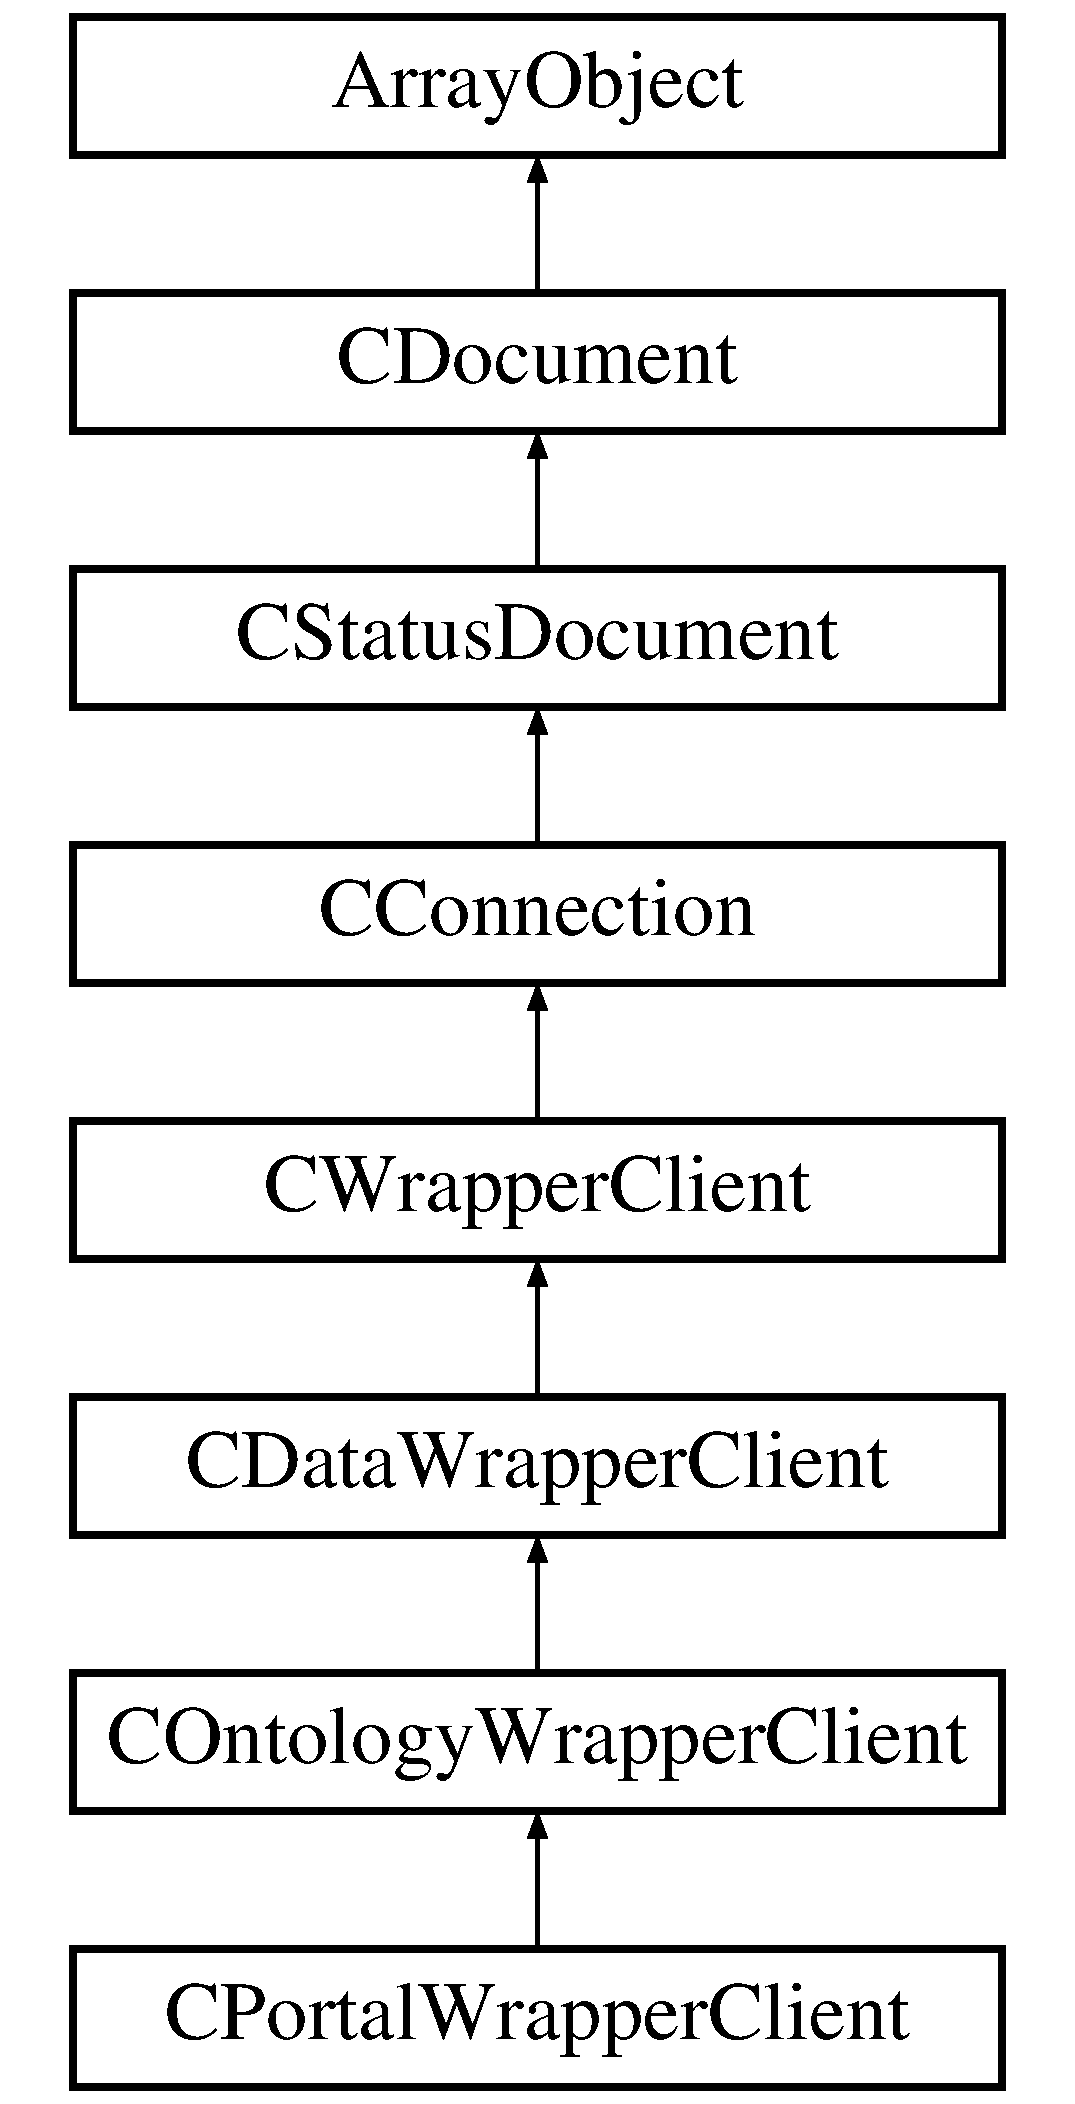
\includegraphics[height=8.000000cm]{class_c_portal_wrapper_client}
\end{center}
\end{figure}
\subsection*{Public Member Functions}
\begin{DoxyCompactItemize}
\item 
\hyperlink{class_c_portal_wrapper_client_aaa306c1d688a07350afc734fcaa60c9d}{Operation} (\$the\-Value=N\-U\-L\-L, \$get\-Old=F\-A\-L\-S\-E)
\item 
\hyperlink{class_c_portal_wrapper_client_a60afce66299dc26e5d51ea48fe944fd7}{Credentials} (\$the\-Key, \$the\-Value=N\-U\-L\-L, \$get\-Old=F\-A\-L\-S\-E)
\end{DoxyCompactItemize}
\subsection*{Protected Member Functions}
\begin{DoxyCompactItemize}
\item 
\hyperlink{class_c_portal_wrapper_client_aa7f24544e1e159c2eefac9b16d3bc41e}{\-\_\-\-Check\-Dependencies} (\$the\-Operation)
\item 
\hyperlink{class_c_portal_wrapper_client_abaa1c93796951da6d4cad14791014de7}{\-\_\-\-Normalise\-Parameters} ()
\item 
\hyperlink{class_c_portal_wrapper_client_a9e354d6ae8398aa27d62cd5b846b24cb}{\-\_\-\-Encode\-Parameters} (\&\$the\-Parameters, \$the\-Encoding)
\end{DoxyCompactItemize}
\subsection*{Additional Inherited Members}


\subsection{Member Function Documentation}
\hypertarget{class_c_portal_wrapper_client_aa7f24544e1e159c2eefac9b16d3bc41e}{\index{C\-Portal\-Wrapper\-Client@{C\-Portal\-Wrapper\-Client}!\-\_\-\-Check\-Dependencies@{\-\_\-\-Check\-Dependencies}}
\index{\-\_\-\-Check\-Dependencies@{\-\_\-\-Check\-Dependencies}!CPortalWrapperClient@{C\-Portal\-Wrapper\-Client}}
\subsubsection[{\-\_\-\-Check\-Dependencies}]{\setlength{\rightskip}{0pt plus 5cm}C\-Portal\-Wrapper\-Client\-::\-\_\-\-Check\-Dependencies (
\begin{DoxyParamCaption}
\item[{}]{\$the\-Operation}
\end{DoxyParamCaption}
)\hspace{0.3cm}{\ttfamily [protected]}}}\label{class_c_portal_wrapper_client_aa7f24544e1e159c2eefac9b16d3bc41e}
Check operation dependencies.

This method can be used to assert whether the required parameters are present depending on the requested operation.


\begin{DoxyParams}[1]{Parameters}
string & {\em \$the\-Operation} & Requested operation.\\
\hline
\end{DoxyParams}
protected


\begin{DoxyExceptions}{Exceptions}
{\em Exception} & \\
\hline
\end{DoxyExceptions}
\hypertarget{class_c_portal_wrapper_client_a9e354d6ae8398aa27d62cd5b846b24cb}{\index{C\-Portal\-Wrapper\-Client@{C\-Portal\-Wrapper\-Client}!\-\_\-\-Encode\-Parameters@{\-\_\-\-Encode\-Parameters}}
\index{\-\_\-\-Encode\-Parameters@{\-\_\-\-Encode\-Parameters}!CPortalWrapperClient@{C\-Portal\-Wrapper\-Client}}
\subsubsection[{\-\_\-\-Encode\-Parameters}]{\setlength{\rightskip}{0pt plus 5cm}C\-Portal\-Wrapper\-Client\-::\-\_\-\-Encode\-Parameters (
\begin{DoxyParamCaption}
\item[{\&}]{\$the\-Parameters, }
\item[{}]{\$the\-Encoding}
\end{DoxyParamCaption}
)\hspace{0.3cm}{\ttfamily [protected]}}}\label{class_c_portal_wrapper_client_a9e354d6ae8398aa27d62cd5b846b24cb}
Encode parameters.

This method can be used to encode parameters before they get sent to the service.

We overload this method to handle the local parameters.


\begin{DoxyParams}[1]{Parameters}
reference & {\em \&\$the\-Parameters} & List of parameters. \\
\hline
string & {\em \$the\-Encoding} & Encoding code.\\
\hline
\end{DoxyParams}
protected \hypertarget{class_c_portal_wrapper_client_abaa1c93796951da6d4cad14791014de7}{\index{C\-Portal\-Wrapper\-Client@{C\-Portal\-Wrapper\-Client}!\-\_\-\-Normalise\-Parameters@{\-\_\-\-Normalise\-Parameters}}
\index{\-\_\-\-Normalise\-Parameters@{\-\_\-\-Normalise\-Parameters}!CPortalWrapperClient@{C\-Portal\-Wrapper\-Client}}
\subsubsection[{\-\_\-\-Normalise\-Parameters}]{\setlength{\rightskip}{0pt plus 5cm}C\-Portal\-Wrapper\-Client\-::\-\_\-\-Normalise\-Parameters (
\begin{DoxyParamCaption}
{}
\end{DoxyParamCaption}
)\hspace{0.3cm}{\ttfamily [protected]}}}\label{class_c_portal_wrapper_client_abaa1c93796951da6d4cad14791014de7}
Normalise parameters.

This method can be used to normalise parameters before they get encoded.

In this class we set the default container name for login.

protected \hypertarget{class_c_portal_wrapper_client_a60afce66299dc26e5d51ea48fe944fd7}{\index{C\-Portal\-Wrapper\-Client@{C\-Portal\-Wrapper\-Client}!Credentials@{Credentials}}
\index{Credentials@{Credentials}!CPortalWrapperClient@{C\-Portal\-Wrapper\-Client}}
\subsubsection[{Credentials}]{\setlength{\rightskip}{0pt plus 5cm}C\-Portal\-Wrapper\-Client\-::\-Credentials (
\begin{DoxyParamCaption}
\item[{}]{\$the\-Key, }
\item[{}]{\$the\-Value = {\ttfamily NULL}, }
\item[{}]{\$get\-Old = {\ttfamily FALSE}}
\end{DoxyParamCaption}
)}}\label{class_c_portal_wrapper_client_a60afce66299dc26e5d51ea48fe944fd7}
Manage user credentials.

This method can be used to manage the \hyperlink{}{k\-A\-P\-I\-\_\-\-C\-R\-E\-D\-E\-N\-T\-I\-A\-L\-S} offset, it accepts the following parameters\-:


\begin{DoxyItemize}
\item {\ttfamily \$the\-Key}\-: This string represents the element key. 
\item {\ttfamily \$the\-Value}\-: This parameter represents the element value or operation\-: 
\begin{DoxyItemize}
\item {\ttfamily N\-U\-L\-L}\-: Return the the value at the provided key. 
\item {\ttfamily F\-A\-L\-S\-E}\-: Delete the value at the provided key. 
\item {\itshape other}\-: Any other type will replace or set the value at the provided key. 
\end{DoxyItemize}
\item {\ttfamily \$get\-Old}\-: Determines what the method will return\-: 
\begin{DoxyItemize}
\item {\ttfamily T\-R\-U\-E}\-: Return the value of the offset {\itshape before} it was eventually modified. 
\item {\ttfamily F\-A\-L\-S\-E}\-: Return the value of the offset {\itshape after} it was eventually modified. 
\end{DoxyItemize}
\end{DoxyItemize}


\begin{DoxyParams}[1]{Parameters}
string & {\em \$the\-Key} & Element key. \\
\hline
mixed & {\em \$the\-Value} & Value or operation. \\
\hline
boolean & {\em \$get\-Old} & T\-R\-U\-E get old value.\\
\hline
\end{DoxyParams}
public \begin{DoxyReturn}{Returns}
mixed
\end{DoxyReturn}
Manage\-Indexed\-Offset()

\begin{DoxySeeAlso}{See Also}
k\-A\-P\-I\-\_\-\-C\-R\-E\-D\-E\-N\-T\-I\-A\-L\-S 
\end{DoxySeeAlso}
\hypertarget{class_c_portal_wrapper_client_aaa306c1d688a07350afc734fcaa60c9d}{\index{C\-Portal\-Wrapper\-Client@{C\-Portal\-Wrapper\-Client}!Operation@{Operation}}
\index{Operation@{Operation}!CPortalWrapperClient@{C\-Portal\-Wrapper\-Client}}
\subsubsection[{Operation}]{\setlength{\rightskip}{0pt plus 5cm}C\-Portal\-Wrapper\-Client\-::\-Operation (
\begin{DoxyParamCaption}
\item[{}]{\$the\-Value = {\ttfamily NULL}, }
\item[{}]{\$get\-Old = {\ttfamily FALSE}}
\end{DoxyParamCaption}
)}}\label{class_c_portal_wrapper_client_aaa306c1d688a07350afc734fcaa60c9d}
Manage operation.

We \hyperlink{class_c_wrapper_client_ae378229fd57b051ddf0e0a7abf599641}{overload} this method to add the following allowed operations\-:


\begin{DoxyItemize}
\item {\itshape \hyperlink{}{k\-A\-P\-I\-\_\-\-O\-P\-\_\-\-Login}}\-: L\-O\-G\-I\-N web-\/service operation, used to return validate user credentials. 
\end{DoxyItemize}


\begin{DoxyParams}[1]{Parameters}
string & {\em \$the\-Value} & Value or operation. \\
\hline
boolean & {\em \$get\-Old} & T\-R\-U\-E get old value.\\
\hline
\end{DoxyParams}
public \begin{DoxyReturn}{Returns}
mixed
\end{DoxyReturn}

\begin{DoxyExceptions}{Exceptions}
{\em \{@link} & \hyperlink{class_c_exception}{C\-Exception} \hyperlink{class_c_exception}{C\-Exception}\}\\
\hline
\end{DoxyExceptions}
C\-Attribute\-::\-Manage\-Offset()

\begin{DoxySeeAlso}{See Also}
k\-A\-P\-I\-\_\-\-O\-P\-E\-R\-A\-T\-I\-O\-N 
\end{DoxySeeAlso}


The documentation for this class was generated from the following file\-:\begin{DoxyCompactItemize}
\item 
/\-Library/\-Web\-Server/\-Library/\-P\-H\-P\-Wrapper/classes/C\-Portal\-Wrapper\-Client.\-php\end{DoxyCompactItemize}

\hypertarget{class_c_query}{\section{C\-Query Class Reference}
\label{class_c_query}\index{C\-Query@{C\-Query}}
}
Inheritance diagram for C\-Query\-:\begin{figure}[H]
\begin{center}
\leavevmode
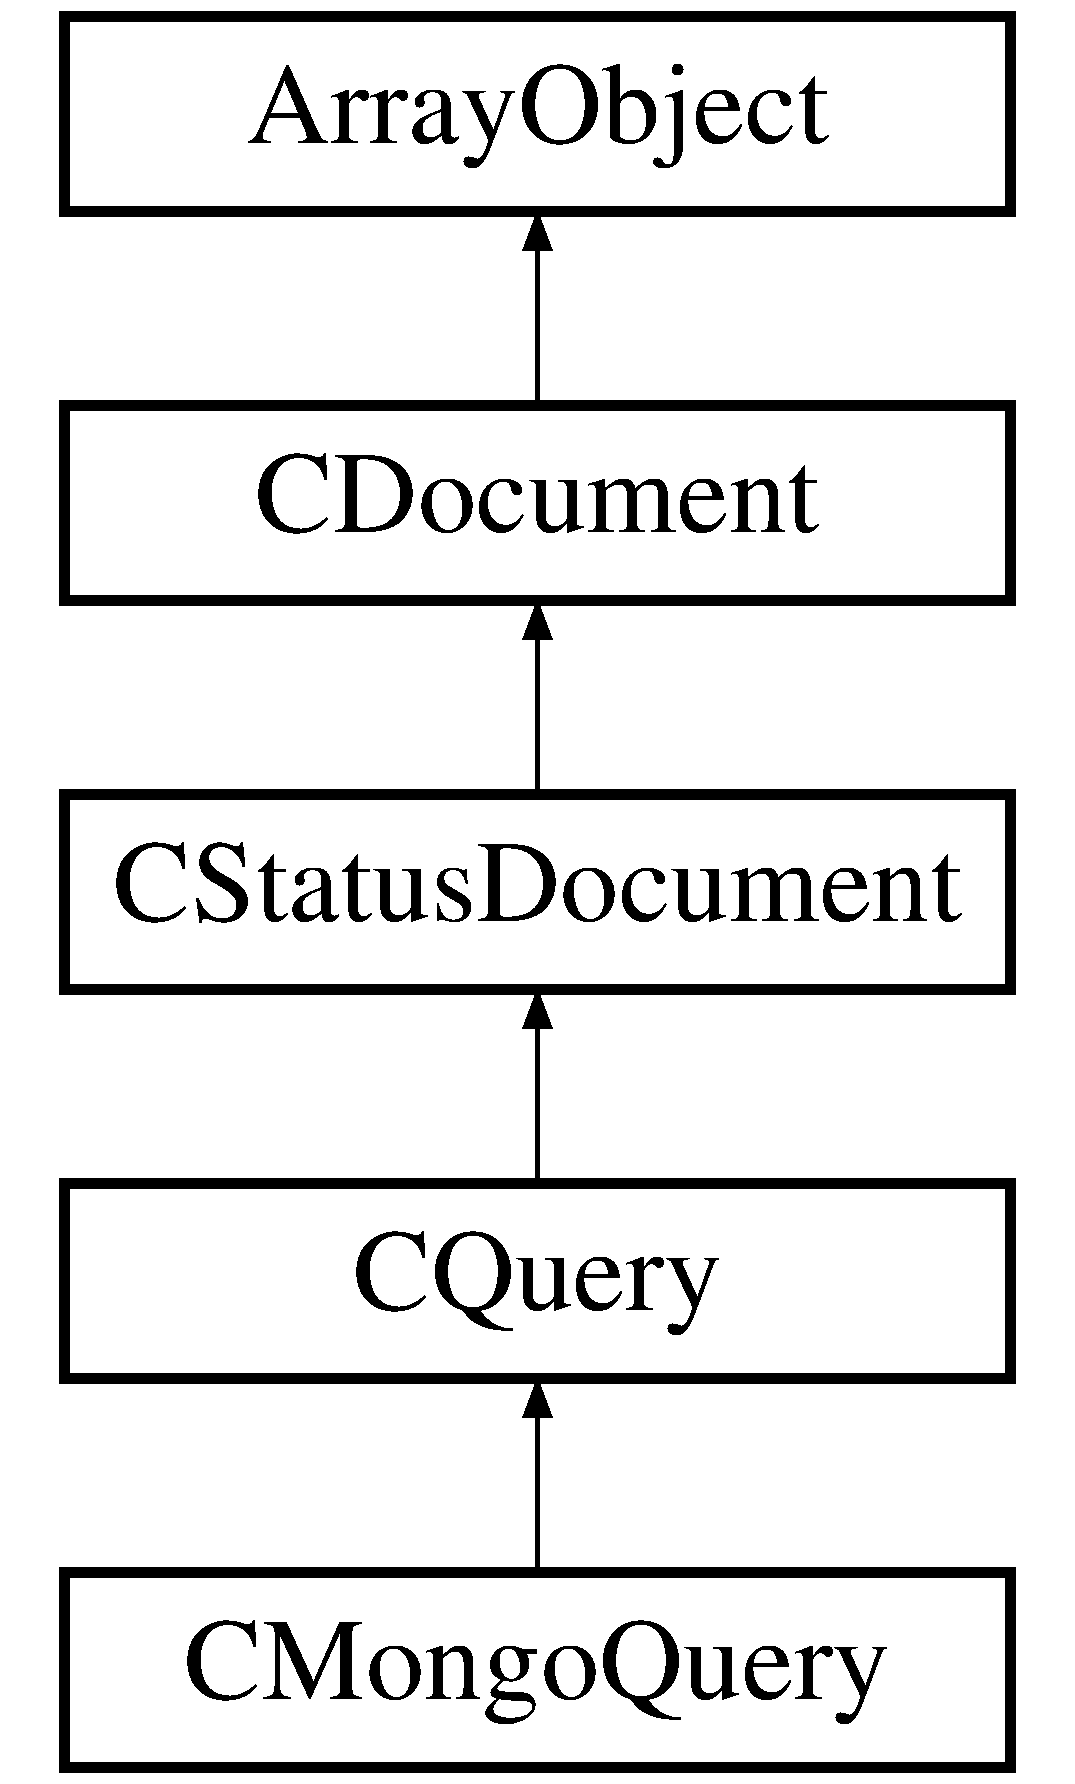
\includegraphics[height=5.000000cm]{class_c_query}
\end{center}
\end{figure}
\subsection*{Public Member Functions}
\begin{DoxyCompactItemize}
\item 
\hyperlink{class_c_query_a5f622c663cffb67955a528cac46502f9}{\-\_\-\-\_\-construct} (\$the\-Query=N\-U\-L\-L)
\item 
\hyperlink{class_c_query_ab18afa41c5060767efc493497f5f82f7}{Append\-Statement} (\$the\-Statement, \$the\-Condition=N\-U\-L\-L)
\item 
\hyperlink{class_c_query_a715ac553707078841213f7b874cbc48e}{Validate} ()
\item 
\hyperlink{class_c_query_a92324584013d5d0b1fd135443d271e19}{Export} (\hyperlink{class_c_connection}{C\-Connection} \$the\-Container)
\end{DoxyCompactItemize}
\subsection*{Protected Member Functions}
\begin{DoxyCompactItemize}
\item 
\hyperlink{class_c_query_aecc479899ce58dec7ad6ab4fc1818971}{\-\_\-\-Handle\-Condition} (\$the\-Query, \$the\-Condition)
\item 
\hyperlink{class_c_query_aa6fb78916ebff1276c0fc06c0510c154}{\-\_\-\-Handle\-Statement} (\$the\-Statement, \$the\-Condition)
\item 
\hyperlink{class_c_query_a1a01d39eedd2951f704dc75c58fb477c}{\-\_\-\-Append\-Statement} (\&\$the\-Query, \$the\-Condition, \$the\-Statement)
\item 
\hyperlink{class_c_query_a5fbde46df4bb30cb252647f0e47cbbde}{\-\_\-\-Validate\-Condition} (\$the\-Condition, \$the\-Statements, \$the\-Level)
\item 
\hyperlink{class_c_query_afe96707c9ed84ee197dae56c9f05f2a4}{\-\_\-\-Validate\-Statement} (\$the\-Statement, \$the\-Level)
\item 
\hyperlink{class_c_query_a257ac2525d848d20b72a92873361e30a}{\-\_\-\-Validate\-Statement\-Operator} (\&\$the\-Statement)
\item 
\hyperlink{class_c_query_aa72fac5ddb123493a4dc0ec3ff145691}{\-\_\-\-Ready} ()
\end{DoxyCompactItemize}
\subsection*{Additional Inherited Members}


\subsection{Constructor \& Destructor Documentation}
\hypertarget{class_c_query_a5f622c663cffb67955a528cac46502f9}{\index{C\-Query@{C\-Query}!\-\_\-\-\_\-construct@{\-\_\-\-\_\-construct}}
\index{\-\_\-\-\_\-construct@{\-\_\-\-\_\-construct}!CQuery@{C\-Query}}
\subsubsection[{\-\_\-\-\_\-construct}]{\setlength{\rightskip}{0pt plus 5cm}C\-Query\-::\-\_\-\-\_\-construct (
\begin{DoxyParamCaption}
\item[{}]{\$the\-Query = {\ttfamily NULL}}
\end{DoxyParamCaption}
)}}\label{class_c_query_a5f622c663cffb67955a528cac46502f9}
\subparagraph*{Instantiate class}

If you omit the parameter the method will instantiate an empty query, if you provide an {\ttfamily array} or {\ttfamily \hyperlink{}{Array\-Object}} it will assume the structure to be a query and will instantiate the object with it; any other data type will raise an exception.


\begin{DoxyParams}[1]{Parameters}
mixed & {\em \$the\-Query} & Query data.\\
\hline
\end{DoxyParams}
public


\begin{DoxyExceptions}{Exceptions}
{\em Exception} & \\
\hline
\end{DoxyExceptions}


\subsection{Member Function Documentation}
\hypertarget{class_c_query_a1a01d39eedd2951f704dc75c58fb477c}{\index{C\-Query@{C\-Query}!\-\_\-\-Append\-Statement@{\-\_\-\-Append\-Statement}}
\index{\-\_\-\-Append\-Statement@{\-\_\-\-Append\-Statement}!CQuery@{C\-Query}}
\subsubsection[{\-\_\-\-Append\-Statement}]{\setlength{\rightskip}{0pt plus 5cm}C\-Query\-::\-\_\-\-Append\-Statement (
\begin{DoxyParamCaption}
\item[{\&}]{\$the\-Query, }
\item[{}]{\$the\-Condition, }
\item[{}]{\$the\-Statement}
\end{DoxyParamCaption}
)\hspace{0.3cm}{\ttfamily [protected]}}}\label{class_c_query_a1a01d39eedd2951f704dc75c58fb477c}
\subparagraph*{Append statement}

This method will append the provided statement to the current query.

Statements of the same type, \hyperlink{}{k\-O\-P\-E\-R\-A\-T\-O\-R\-\_\-\-A\-N\-D} and \hyperlink{}{k\-O\-P\-E\-R\-A\-T\-O\-R\-\_\-\-N\-A\-N\-D}, or \hyperlink{}{k\-O\-P\-E\-R\-A\-T\-O\-R\-\_\-\-O\-R} and \hyperlink{}{k\-O\-P\-E\-R\-A\-T\-O\-R\-\_\-\-N\-O\-R}, will be added at the same level. If the top level is an \hyperlink{}{k\-O\-P\-E\-R\-A\-T\-O\-R\-\_\-\-O\-R} or \hyperlink{}{k\-O\-P\-E\-R\-A\-T\-O\-R\-\_\-\-N\-O\-R} and the provided statement is an \hyperlink{}{k\-O\-P\-E\-R\-A\-T\-O\-R\-\_\-\-A\-N\-D} or \hyperlink{}{k\-O\-P\-E\-R\-A\-T\-O\-R\-\_\-\-N\-A\-N\-D}, the latter will be promoted to the top level.

The parameters to this method are\-:


\begin{DoxyItemize}
\item {\ttfamily \&\$the\-Query}\-: Query receiving statement. 
\item {\ttfamily \$the\-Condition}\-: Statement condition. 
\item {\ttfamily \$the\-Condition}\-: Boolean statement condition code. 
\end{DoxyItemize}


\begin{DoxyParams}[1]{Parameters}
reference & {\em \&\$the\-Query} & Query. \\
\hline
array & {\em \$the\-Condition} & Statement condition. \\
\hline
string & {\em \$the\-Statement} & Statement.\\
\hline
\end{DoxyParams}
protected \hypertarget{class_c_query_aecc479899ce58dec7ad6ab4fc1818971}{\index{C\-Query@{C\-Query}!\-\_\-\-Handle\-Condition@{\-\_\-\-Handle\-Condition}}
\index{\-\_\-\-Handle\-Condition@{\-\_\-\-Handle\-Condition}!CQuery@{C\-Query}}
\subsubsection[{\-\_\-\-Handle\-Condition}]{\setlength{\rightskip}{0pt plus 5cm}C\-Query\-::\-\_\-\-Handle\-Condition (
\begin{DoxyParamCaption}
\item[{}]{\$the\-Query, }
\item[{}]{\$the\-Condition}
\end{DoxyParamCaption}
)\hspace{0.3cm}{\ttfamily [protected]}}}\label{class_c_query_aecc479899ce58dec7ad6ab4fc1818971}
\subparagraph*{Handle condition}

This method will chain the provided query to the current query, it expects the first parameter to be a query array and the second parameter to be the condition that will be used to chain the provided query to the current query.

The process of combining queries is governed by a set of three conditions\-: the {\itshape current} query condition, the {\itshape provided} condition and the {\itshape statement} condition. These conditions are compared as follows\-:


\begin{DoxyItemize}
\item {\ttfamily \hyperlink{}{k\-O\-P\-E\-R\-A\-T\-O\-R\-\_\-\-O\-R}} is equivalent to {\ttfamily \hyperlink{}{k\-O\-P\-E\-R\-A\-T\-O\-R\-\_\-\-N\-O\-R}}. 
\item {\ttfamily \hyperlink{}{k\-O\-P\-E\-R\-A\-T\-O\-R\-\_\-\-A\-N\-D}} is equivalent to {\ttfamily \hyperlink{}{k\-O\-P\-E\-R\-A\-T\-O\-R\-\_\-\-N\-A\-N\-D}}. 
\end{DoxyItemize}

Depending on the combination of these three conditions\-:


\begin{DoxyItemize}
\item {\itshape current} = {\itshape provided} = {\itshape statement}\-: The provided query statements are recursively sent to the \hyperlink{class_c_query_ab18afa41c5060767efc493497f5f82f7}{Append\-Statement()} method using the condition of the provided {\itshape statement}. 
\item {\itshape current} = {\itshape provided}\-: The provided query is appended to the current query. 
\item {\itshape current} = {\itshape statement}\-: A new empty query is created by appending the old current query and the provided query using the provided condition. 
\item {\itshape provided} = {\itshape statement}\-: The current query is appended to the provided query. 
\end{DoxyItemize}


\begin{DoxyParams}[1]{Parameters}
array & {\em \$the\-Query} & Query. \\
\hline
string & {\em \$the\-Condition} & Query condition.\\
\hline
\end{DoxyParams}
protected \hypertarget{class_c_query_aa6fb78916ebff1276c0fc06c0510c154}{\index{C\-Query@{C\-Query}!\-\_\-\-Handle\-Statement@{\-\_\-\-Handle\-Statement}}
\index{\-\_\-\-Handle\-Statement@{\-\_\-\-Handle\-Statement}!CQuery@{C\-Query}}
\subsubsection[{\-\_\-\-Handle\-Statement}]{\setlength{\rightskip}{0pt plus 5cm}C\-Query\-::\-\_\-\-Handle\-Statement (
\begin{DoxyParamCaption}
\item[{}]{\$the\-Statement, }
\item[{}]{\$the\-Condition}
\end{DoxyParamCaption}
)\hspace{0.3cm}{\ttfamily [protected]}}}\label{class_c_query_aa6fb78916ebff1276c0fc06c0510c154}
\subparagraph*{Handle statement}

This method will append the provided statement to the current query, it will handle the provided statement as a single scalar statement.


\begin{DoxyParams}[1]{Parameters}
array & {\em \$the\-Statement} & Statement. \\
\hline
string & {\em \$the\-Condition} & Statement condition.\\
\hline
\end{DoxyParams}
protected \hypertarget{class_c_query_aa72fac5ddb123493a4dc0ec3ff145691}{\index{C\-Query@{C\-Query}!\-\_\-\-Ready@{\-\_\-\-Ready}}
\index{\-\_\-\-Ready@{\-\_\-\-Ready}!CQuery@{C\-Query}}
\subsubsection[{\-\_\-\-Ready}]{\setlength{\rightskip}{0pt plus 5cm}C\-Query\-::\-\_\-\-Ready (
\begin{DoxyParamCaption}
{}
\end{DoxyParamCaption}
)\hspace{0.3cm}{\ttfamily [protected]}}}\label{class_c_query_aa72fac5ddb123493a4dc0ec3ff145691}
\subparagraph*{Determine if the object is ready}

In this class the method will return {\ttfamily T\-R\-U\-E} if the current object has at least one offset set, an indication that it holds a query.

protected \begin{DoxyReturn}{Returns}
boolean {\ttfamily T\-R\-U\-E} means \hyperlink{}{. }
\end{DoxyReturn}
\hypertarget{class_c_query_a5fbde46df4bb30cb252647f0e47cbbde}{\index{C\-Query@{C\-Query}!\-\_\-\-Validate\-Condition@{\-\_\-\-Validate\-Condition}}
\index{\-\_\-\-Validate\-Condition@{\-\_\-\-Validate\-Condition}!CQuery@{C\-Query}}
\subsubsection[{\-\_\-\-Validate\-Condition}]{\setlength{\rightskip}{0pt plus 5cm}C\-Query\-::\-\_\-\-Validate\-Condition (
\begin{DoxyParamCaption}
\item[{}]{\$the\-Condition, }
\item[{}]{\$the\-Statements, }
\item[{}]{\$the\-Level}
\end{DoxyParamCaption}
)\hspace{0.3cm}{\ttfamily [protected]}}}\label{class_c_query_a5fbde46df4bb30cb252647f0e47cbbde}
\subparagraph*{Validate condition}

This method expects a condition as its argument, it will check if it is a valid condition, then it will validate all condition statements.


\begin{DoxyParams}[1]{Parameters}
string & {\em \$the\-Condition} & Boolean condition. \\
\hline
array & {\em \$the\-Statements} & Statements list. \\
\hline
integer & {\em \$the\-Level} & \mbox{[}P\-R\-I\-V\-A\-T\-E\mbox{]} condition level.\\
\hline
\end{DoxyParams}
protected


\begin{DoxyExceptions}{Exceptions}
{\em Exception} & \hyperlink{class_c_query_afe96707c9ed84ee197dae56c9f05f2a4}{\-\_\-\-Validate\-Statement()} \\
\hline
\end{DoxyExceptions}
\hypertarget{class_c_query_afe96707c9ed84ee197dae56c9f05f2a4}{\index{C\-Query@{C\-Query}!\-\_\-\-Validate\-Statement@{\-\_\-\-Validate\-Statement}}
\index{\-\_\-\-Validate\-Statement@{\-\_\-\-Validate\-Statement}!CQuery@{C\-Query}}
\subsubsection[{\-\_\-\-Validate\-Statement}]{\setlength{\rightskip}{0pt plus 5cm}C\-Query\-::\-\_\-\-Validate\-Statement (
\begin{DoxyParamCaption}
\item[{}]{\$the\-Statement, }
\item[{}]{\$the\-Level}
\end{DoxyParamCaption}
)\hspace{0.3cm}{\ttfamily [protected]}}}\label{class_c_query_afe96707c9ed84ee197dae56c9f05f2a4}
\subparagraph*{Validate statement}

This method expects a statement as its argument, it will check if it is a valid statement and check if all required elements are there.


\begin{DoxyParams}[1]{Parameters}
array & {\em \$the\-Statement} & Statement. \\
\hline
integer & {\em \$the\-Level} & \mbox{[}P\-R\-I\-V\-A\-T\-E\mbox{]} condition level.\\
\hline
\end{DoxyParams}
protected


\begin{DoxyExceptions}{Exceptions}
{\em Exception} & \hyperlink{class_c_query_a5fbde46df4bb30cb252647f0e47cbbde}{\-\_\-\-Validate\-Condition()} \\
\hline
\end{DoxyExceptions}
\hypertarget{class_c_query_a257ac2525d848d20b72a92873361e30a}{\index{C\-Query@{C\-Query}!\-\_\-\-Validate\-Statement\-Operator@{\-\_\-\-Validate\-Statement\-Operator}}
\index{\-\_\-\-Validate\-Statement\-Operator@{\-\_\-\-Validate\-Statement\-Operator}!CQuery@{C\-Query}}
\subsubsection[{\-\_\-\-Validate\-Statement\-Operator}]{\setlength{\rightskip}{0pt plus 5cm}C\-Query\-::\-\_\-\-Validate\-Statement\-Operator (
\begin{DoxyParamCaption}
\item[{\&}]{\$the\-Statement}
\end{DoxyParamCaption}
)\hspace{0.3cm}{\ttfamily [protected]}}}\label{class_c_query_a257ac2525d848d20b72a92873361e30a}
\subparagraph*{Validate statement operator}

This method expects the statement reference, it will raise an exception if the operator is not supported and if the statement is missing required properties according to the operator.


\begin{DoxyParams}[1]{Parameters}
reference & {\em \&\$the\-Statement} & Statement.\\
\hline
\end{DoxyParams}
protected


\begin{DoxyExceptions}{Exceptions}
{\em Exception} & \\
\hline
\end{DoxyExceptions}
\hypertarget{class_c_query_ab18afa41c5060767efc493497f5f82f7}{\index{C\-Query@{C\-Query}!Append\-Statement@{Append\-Statement}}
\index{Append\-Statement@{Append\-Statement}!CQuery@{C\-Query}}
\subsubsection[{Append\-Statement}]{\setlength{\rightskip}{0pt plus 5cm}C\-Query\-::\-Append\-Statement (
\begin{DoxyParamCaption}
\item[{}]{\$the\-Statement, }
\item[{}]{\$the\-Condition = {\ttfamily NULL}}
\end{DoxyParamCaption}
)}}\label{class_c_query_ab18afa41c5060767efc493497f5f82f7}
\subparagraph*{Append statement}

This method will append the provided statement or query to the current query.

The first parameter is expected to be either a single statement or a query which is represented by a collection of statements chained by a condition.

The method expects the first parameter to be either an object derived from \hyperlink{class_c_query_statement}{C\-Query\-Statement}, an object derived from this class or an array.

If the current key of the provided statement matches one of the standard conditions (\hyperlink{}{k\-O\-P\-E\-R\-A\-T\-O\-R\-\_\-\-A\-N\-D}, \hyperlink{}{k\-O\-P\-E\-R\-A\-T\-O\-R\-\_\-\-N\-A\-N\-D}, \hyperlink{}{k\-O\-P\-E\-R\-A\-T\-O\-R\-\_\-\-O\-R} or \hyperlink{}{k\-O\-P\-E\-R\-A\-T\-O\-R\-\_\-\-N\-O\-R}), it is assumed that the provided statement is a {\itshape query}; if that is not the case, it is assumed that the provided statement is a single or collection of {\itshape statements}.


\begin{DoxyItemize}
\item {\itshape Statement}\-: The provided statement will be appended to the current query; see the \hyperlink{class_c_query_aa6fb78916ebff1276c0fc06c0510c154}{\-\_\-\-Handle\-Statement()} method for more details. 
\begin{DoxyItemize}
\item {\itshape Condition provided}\-: 
\begin{DoxyItemize}
\item {\itshape Current query is empty}\-: The statement and the condition will become the current query. 
\item {\itshape Current query is not empty}\-: The statement will be appended to the current query using the provided condition. 
\end{DoxyItemize}
\item {\itshape Condition not provided}\-: The condition will be determined\-: 
\begin{DoxyItemize}
\item {\itshape Current query is empty}\-: The condition will default to \hyperlink{}{k\-O\-P\-E\-R\-A\-T\-O\-R\-\_\-\-A\-N\-D}. 
\item {\itshape Current query is not empty}\-: The current query condition will be used. 
\end{DoxyItemize}
\end{DoxyItemize}
\item {\itshape Query}\-: The provided query will be chained to the current query; see the \hyperlink{class_c_query_aecc479899ce58dec7ad6ab4fc1818971}{\-\_\-\-Handle\-Condition()} method for more details. 
\begin{DoxyItemize}
\item {\itshape Condition provided}\-: 
\begin{DoxyItemize}
\item {\itshape Current query is empty}\-: The provided query will become the current query and the provided condition will be ignored. 
\item {\itshape Current query is not empty}\-: The provided query will be chained to the current query using the provided condition. 
\end{DoxyItemize}
\item {\itshape Condition not provided}\-: 
\begin{DoxyItemize}
\item {\itshape Current query is empty}\-: The provided query will become the current query. 
\item {\itshape Current query is not empty}\-: The current query condition will be used. 
\end{DoxyItemize}
\end{DoxyItemize}
\end{DoxyItemize}

This method makes use of two protected method for doing the dirty job\-: \hyperlink{class_c_query_aecc479899ce58dec7ad6ab4fc1818971}{\-\_\-\-Handle\-Condition()} for queries and \hyperlink{class_c_query_aa6fb78916ebff1276c0fc06c0510c154}{\-\_\-\-Handle\-Statement()} for statements.

{\itshape Note\-: Try not to mix \hyperlink{}{k\-O\-P\-E\-R\-A\-T\-O\-R\-\_\-\-O\-R} with \hyperlink{}{k\-O\-P\-E\-R\-A\-T\-O\-R\-\_\-\-N\-O\-R} or \hyperlink{}{k\-O\-P\-E\-R\-A\-T\-O\-R\-\_\-\-A\-N\-D} and \hyperlink{}{k\-O\-P\-E\-R\-A\-T\-O\-R\-\_\-\-N\-A\-N\-D} when adding queries, the methods that join queries do not yet handle these combinations well\-: only mix them when adding statements.}


\begin{DoxyParams}[1]{Parameters}
array & {\em \$the\-Statement} & Statement. \\
\hline
string & {\em \$the\-Condition} & Statement condition.\\
\hline
\end{DoxyParams}
public \hypertarget{class_c_query_a92324584013d5d0b1fd135443d271e19}{\index{C\-Query@{C\-Query}!Export@{Export}}
\index{Export@{Export}!CQuery@{C\-Query}}
\subsubsection[{Export}]{\setlength{\rightskip}{0pt plus 5cm}C\-Query\-::\-Export (
\begin{DoxyParamCaption}
\item[{{\bf C\-Connection}}]{\$the\-Container}
\end{DoxyParamCaption}
)}}\label{class_c_query_a92324584013d5d0b1fd135443d271e19}
\subparagraph*{Export query}

The method will return an array suitable to be provided as a native query, the method requires a container that will take care of converting query arguments to native data types.

In this class we simply return the query as it is.


\begin{DoxyParams}[1]{Parameters}
\hyperlink{class_c_connection}{C\-Connection} & {\em \$the\-Container} & Query container.\\
\hline
\end{DoxyParams}
public \begin{DoxyReturn}{Returns}
array
\end{DoxyReturn}

\begin{DoxyExceptions}{Exceptions}
{\em Exception} & \\
\hline
\end{DoxyExceptions}
\hypertarget{class_c_query_a715ac553707078841213f7b874cbc48e}{\index{C\-Query@{C\-Query}!Validate@{Validate}}
\index{Validate@{Validate}!CQuery@{C\-Query}}
\subsubsection[{Validate}]{\setlength{\rightskip}{0pt plus 5cm}C\-Query\-::\-Validate (
\begin{DoxyParamCaption}
{}
\end{DoxyParamCaption}
)}}\label{class_c_query_a715ac553707078841213f7b874cbc48e}
\subparagraph*{Validate query}

This method will check whether the query structure is valid.

public

\hyperlink{class_c_query_a5fbde46df4bb30cb252647f0e47cbbde}{\-\_\-\-Validate\-Condition()} 

The documentation for this class was generated from the following file\-:\begin{DoxyCompactItemize}
\item 
/\-Library/\-Web\-Server/\-Library/\-P\-H\-P\-Wrapper/classes/C\-Query.\-php\end{DoxyCompactItemize}

\hypertarget{class_c_query_statement}{\section{C\-Query\-Statement Class Reference}
\label{class_c_query_statement}\index{C\-Query\-Statement@{C\-Query\-Statement}}
}
Inheritance diagram for C\-Query\-Statement\-:\begin{figure}[H]
\begin{center}
\leavevmode
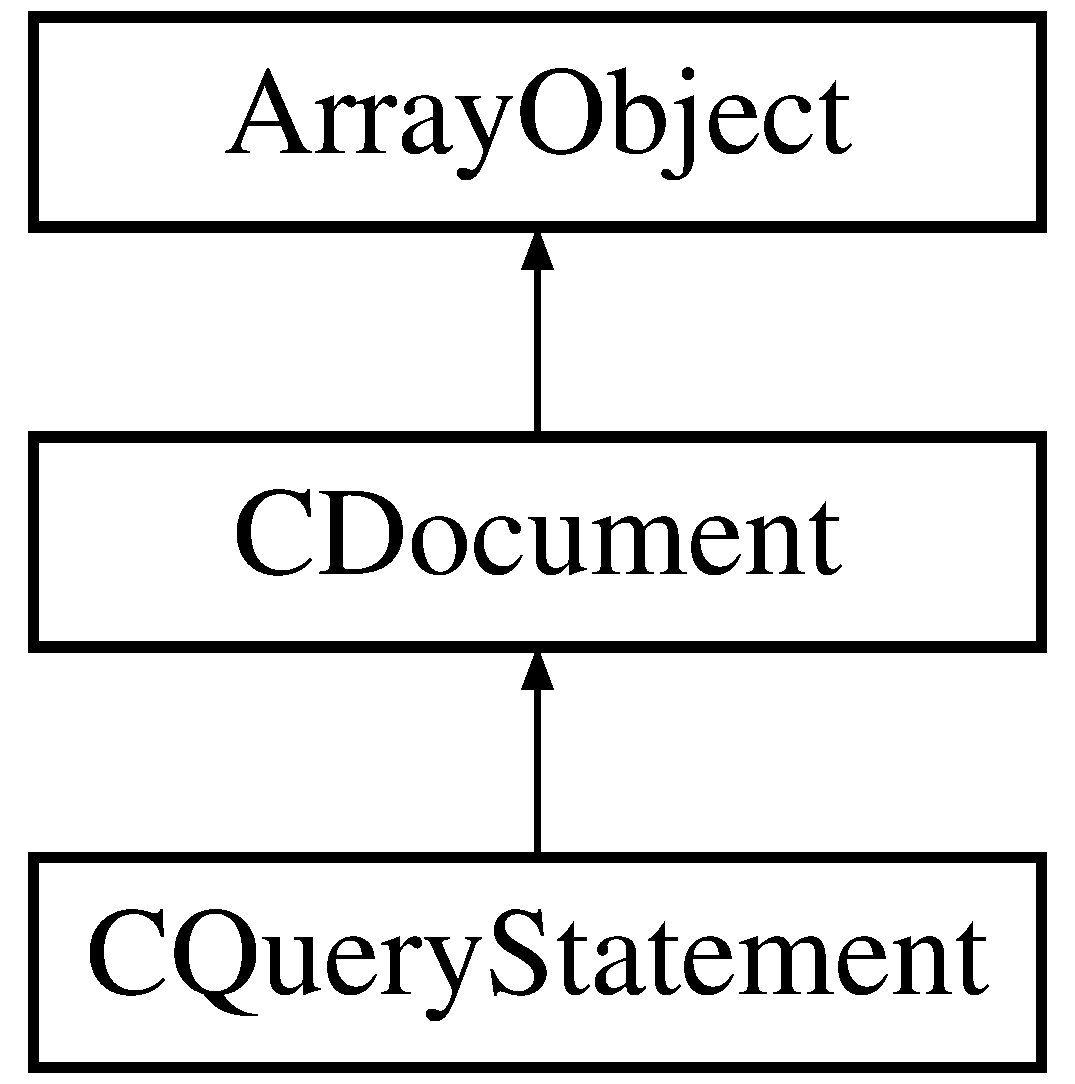
\includegraphics[height=3.000000cm]{class_c_query_statement}
\end{center}
\end{figure}
\subsection*{Public Member Functions}
\begin{DoxyCompactItemize}
\item 
\hyperlink{class_c_query_statement_a996b7a9ae1d54bc3f73de41501b5e02b}{\-\_\-\-\_\-construct} (\$the\-Subject=N\-U\-L\-L, \$the\-Predicate=N\-U\-L\-L, \$the\-Type=N\-U\-L\-L, \$the\-Object=N\-U\-L\-L, \$the\-Range=N\-U\-L\-L)
\item 
\hyperlink{class_c_query_statement_a5a27c44c892286e2fc77dc961d2e30d4}{Subject} (\$the\-Value=N\-U\-L\-L, \$get\-Old=F\-A\-L\-S\-E)
\item 
\hyperlink{class_c_query_statement_ae941698661c8f4b94ce08ea1eaad94b7}{Object} (\$the\-Value=N\-U\-L\-L, \$get\-Old=F\-A\-L\-S\-E)
\item 
\hyperlink{class_c_query_statement_a4a6c6eca496b006e21bfd9c18a31f116}{Predicate} (\$the\-Value=N\-U\-L\-L, \$get\-Old=F\-A\-L\-S\-E)
\item 
\hyperlink{class_c_query_statement_a37bbaad291c18c92954cc25dd49c117b}{Type} (\$the\-Value=N\-U\-L\-L, \$get\-Old=F\-A\-L\-S\-E)
\item 
\hyperlink{class_c_query_statement_a17cf641a4180129015bc0da8e83a7a4c}{Range} (\$the\-Bound1, \$the\-Bound2, \$get\-Old=F\-A\-L\-S\-E)
\end{DoxyCompactItemize}
\subsection*{Static Public Member Functions}
\begin{DoxyCompactItemize}
\item 
static \hyperlink{class_c_query_statement_ac14041ddd7df1cca53aa6594aac7872f}{Disabled} (\$the\-Subject, \$the\-Object=N\-U\-L\-L, \$the\-Type=N\-U\-L\-L, \$the\-Range=N\-U\-L\-L)
\item 
static \hyperlink{class_c_query_statement_a37f7b088b60623ba9435fc400276a828}{Equals} (\$the\-Subject, \$the\-Object, \$the\-Type=N\-U\-L\-L)
\item 
static \hyperlink{class_c_query_statement_a3152dfb1a2eda4047a11ffcd2af50846}{Not\-Equals} (\$the\-Subject, \$the\-Object, \$the\-Type=N\-U\-L\-L)
\item 
static \hyperlink{class_c_query_statement_a26fd9aefa3c9df4228f9aaa7b5d74cbc}{Like} (\$the\-Subject, \$the\-Object)
\item 
static \hyperlink{class_c_query_statement_a6c89cfdf83f46e2fd3ca807254236ed7}{Not\-Like} (\$the\-Subject, \$the\-Object)
\item 
static \hyperlink{class_c_query_statement_a343902e7ebf9facbff20bcd9be63794c}{Prefix} (\$the\-Subject, \$the\-Object)
\item 
static \hyperlink{class_c_query_statement_a30153cce507070c5dc56a1facaaf6059}{Prefix\-No\-Case} (\$the\-Subject, \$the\-Object)
\item 
static \hyperlink{class_c_query_statement_abdc4fa447abbde5aa34959f6b830a7e0}{Contains} (\$the\-Subject, \$the\-Object)
\item 
static \hyperlink{class_c_query_statement_add86e9e2ddf11114e53f0765b9dd85d8}{Contains\-No\-Case} (\$the\-Subject, \$the\-Object)
\item 
static \hyperlink{class_c_query_statement_a80232c348a9db646d3a94bd44611918e}{Suffix} (\$the\-Subject, \$the\-Object)
\item 
static \hyperlink{class_c_query_statement_a25c7240b6ace38d7839fc5bc363505ec}{Suffix\-No\-Case} (\$the\-Subject, \$the\-Object)
\item 
static \hyperlink{class_c_query_statement_a952e2d252c4a2a469c03a9e96f151d35}{Regex} (\$the\-Subject, \$the\-Object)
\item 
static \hyperlink{class_c_query_statement_af3a8b31af7f32562fb1ce7ba16f69766}{Less} (\$the\-Subject, \$the\-Object, \$the\-Type=N\-U\-L\-L)
\item 
static \hyperlink{class_c_query_statement_a292880d593cc8b46dba77d13004aaa28}{Less\-Equal} (\$the\-Subject, \$the\-Object, \$the\-Type=N\-U\-L\-L)
\item 
static \hyperlink{class_c_query_statement_abe09c835887534aeecbeffad2045c917}{Great} (\$the\-Subject, \$the\-Object, \$the\-Type=N\-U\-L\-L)
\item 
static \hyperlink{class_c_query_statement_a540d93d646384d5a145d3944d72246e3}{Great\-Equal} (\$the\-Subject, \$the\-Object, \$the\-Type=N\-U\-L\-L)
\item 
static \hyperlink{class_c_query_statement_ae18f91d3c6c1ad07bb380d959ce01c1b}{Range\-Inclusive} (\$the\-Subject, \$the\-Bound1, \$the\-Bound2, \$the\-Type=N\-U\-L\-L)
\item 
static \hyperlink{class_c_query_statement_a182c44c738d574e6d331d5bd894ce8e7}{Range\-Exclusive} (\$the\-Subject, \$the\-Bound1, \$the\-Bound2, \$the\-Type=N\-U\-L\-L)
\item 
static \hyperlink{class_c_query_statement_a45c462050093bf18a5065cb018c91a34}{Missing} (\$the\-Subject)
\item 
static \hyperlink{class_c_query_statement_aba90304323e0de3966810bf1bed26ef4}{Exists} (\$the\-Subject)
\item 
static \hyperlink{class_c_query_statement_a5e1a291d73a20b4f88c019d1863a4c81}{Member} (\$the\-Subject, \$the\-Object, \$the\-Type=N\-U\-L\-L)
\item 
static \hyperlink{class_c_query_statement_aeb90f2ea2237ddc0ab01d9965538abf4}{Not\-Member} (\$the\-Subject, \$the\-Object, \$the\-Type=N\-U\-L\-L)
\item 
static \hyperlink{class_c_query_statement_a7cb662f303eb30652460fd4903053ca8}{All} (\$the\-Subject, \$the\-Object, \$the\-Type=N\-U\-L\-L)
\item 
static \hyperlink{class_c_query_statement_ac3c86273637210e1d117cae10ff9bfe9}{Not\-All} (\$the\-Subject, \$the\-Object, \$the\-Type=N\-U\-L\-L)
\item 
static \hyperlink{class_c_query_statement_ae668b0a35863ac739a188cecd84027a5}{Expression} (\$the\-Subject, \$the\-Object)
\item 
static \hyperlink{class_c_query_statement_a4427bfe3eff17ec663ecf7a5f77c23d8}{Handle\-Data\-Type} (\&\$the\-Type, \&\$the\-Value)
\end{DoxyCompactItemize}


\subsection{Constructor \& Destructor Documentation}
\hypertarget{class_c_query_statement_a996b7a9ae1d54bc3f73de41501b5e02b}{\index{C\-Query\-Statement@{C\-Query\-Statement}!\-\_\-\-\_\-construct@{\-\_\-\-\_\-construct}}
\index{\-\_\-\-\_\-construct@{\-\_\-\-\_\-construct}!CQueryStatement@{C\-Query\-Statement}}
\subsubsection[{\-\_\-\-\_\-construct}]{\setlength{\rightskip}{0pt plus 5cm}C\-Query\-Statement\-::\-\_\-\-\_\-construct (
\begin{DoxyParamCaption}
\item[{}]{\$the\-Subject = {\ttfamily NULL}, }
\item[{}]{\$the\-Predicate = {\ttfamily NULL}, }
\item[{}]{\$the\-Type = {\ttfamily NULL}, }
\item[{}]{\$the\-Object = {\ttfamily NULL}, }
\item[{}]{\$the\-Range = {\ttfamily NULL}}
\end{DoxyParamCaption}
)}}\label{class_c_query_statement_a996b7a9ae1d54bc3f73de41501b5e02b}
\subparagraph*{Instantiate class}

The constructor can be used to instantiate a statement either by providing an existing statement structure, or by providing the statement elements\-:


\begin{DoxyItemize}
\item {\ttfamily \$the\-Subject}\-: The statement subject\-: 
\begin{DoxyItemize}
\item {\ttfamily array} or {\ttfamily \hyperlink{}{Array\-Object}}\-: Structures are interpreted as built statements, so the method will scan the structure and load the corresponding elements. 
\item {\ttfamily string}\-: Any other type will be converted to a string and interpreted as the statement subject, or data element key. 
\end{DoxyItemize}
\item {\ttfamily \$the\-Predicate}\-: The statement operator or predicate\-: 
\begin{DoxyItemize}
\item {\itshape \hyperlink{}{k\-O\-P\-E\-R\-A\-T\-O\-R\-\_\-\-D\-I\-S\-A\-B\-L\-E\-D}}\-: Disabled, it means that the current statement is disabled; the remaining parameters are ignored. 
\item {\itshape \hyperlink{}{k\-O\-P\-E\-R\-A\-T\-O\-R\-\_\-\-E\-Q\-U\-A\-L}}\-: Equality ({\ttfamily =}), this operator implies that the method expects the next two parameters. 
\item {\itshape \hyperlink{}{k\-O\-P\-E\-R\-A\-T\-O\-R\-\_\-\-E\-Q\-U\-A\-L\-\_\-\-N\-O\-T}}\-: Inequality ({\ttfamily !=}), negates the \hyperlink{}{k\-O\-P\-E\-R\-A\-T\-O\-R\-\_\-\-E\-Q\-U\-A\-L} operator; this operator implies that the method expects the next two parameters. 
\item {\itshape \hyperlink{}{k\-O\-P\-E\-R\-A\-T\-O\-R\-\_\-\-L\-I\-K\-E}}\-: Like, it is an accent and case insensitive equality filter, this operator implies that the method expects the next two parameters. 
\item {\itshape \hyperlink{}{k\-O\-P\-E\-R\-A\-T\-O\-R\-\_\-\-L\-I\-K\-E\-\_\-\-N\-O\-T}}\-: The negation of the \hyperlink{}{k\-O\-P\-E\-R\-A\-T\-O\-R\-\_\-\-L\-I\-K\-E} operator, this operator implies that the method expects the next two parameters. 
\item {\itshape \hyperlink{}{k\-O\-P\-E\-R\-A\-T\-O\-R\-\_\-\-P\-R\-E\-F\-I\-X}}\-: Starts with, or prefix match, this operator implies that the method expects the next two parameters. 
\item {\itshape \hyperlink{}{k\-O\-P\-E\-R\-A\-T\-O\-R\-\_\-\-C\-O\-N\-T\-A\-I\-N\-S}}\-: Contains, selects all elements that contain the match string, this operator implies that the method expects the next two parameters. 
\item {\itshape \hyperlink{}{k\-O\-P\-E\-R\-A\-T\-O\-R\-\_\-\-S\-U\-F\-F\-I\-X}}\-: Ends with, or suffix match, this operator implies that the method expects the next two parameters. 
\item {\itshape \hyperlink{}{k\-O\-P\-E\-R\-A\-T\-O\-R\-\_\-\-R\-E\-G\-E\-X}}\-: Regular expression, this operator implies that the method expects the next two parameters. 
\item {\itshape \hyperlink{}{k\-O\-P\-E\-R\-A\-T\-O\-R\-\_\-\-L\-E\-S\-S}}\-: Smaller than ({\ttfamily $<$}), this operator implies that the method expects the next two parameters. 
\item {\itshape \hyperlink{}{k\-O\-P\-E\-R\-A\-T\-O\-R\-\_\-\-L\-E\-S\-S\-\_\-\-E\-Q\-U\-A\-L}}\-: Smaller than or equal ({\ttfamily $<$=}), this operator implies that the method expects the next two parameters. 
\item {\itshape \hyperlink{}{k\-O\-P\-E\-R\-A\-T\-O\-R\-\_\-\-G\-R\-E\-A\-T}}\-: Greater than ({\ttfamily $>$}), this operator implies that the method expects the next two parameters. 
\item {\itshape \hyperlink{}{k\-O\-P\-E\-R\-A\-T\-O\-R\-\_\-\-G\-R\-E\-A\-T\-\_\-\-E\-Q\-U\-A\-L}}\-: Greater than or equal ({\ttfamily $>$=}), this operator implies that the method expects the next two parameters. 
\item {\itshape \hyperlink{}{k\-O\-P\-E\-R\-A\-T\-O\-R\-\_\-\-I\-R\-A\-N\-G\-E}}\-: Range inclusive, matches {\ttfamily $>$= value $<$=}; this operator implies that the method expects the next three parameters. 
\item {\itshape \hyperlink{}{k\-O\-P\-E\-R\-A\-T\-O\-R\-\_\-\-E\-R\-A\-N\-G\-E}}\-: Range exclusive, matches {\ttfamily $>$ value $<$}, this operator implies that the method expects the next three parameters. 
\item {\itshape \hyperlink{}{k\-O\-P\-E\-R\-A\-T\-O\-R\-\_\-\-N\-U\-L\-L}}\-: Is {\itshape N\-U\-L\-L} or element is missing. 
\item {\itshape \hyperlink{}{k\-O\-P\-E\-R\-A\-T\-O\-R\-\_\-\-N\-O\-T\-\_\-\-N\-U\-L\-L}}\-:Not {\itshape N\-U\-L\-L} or element exists. 
\item {\itshape \hyperlink{}{k\-O\-P\-E\-R\-A\-T\-O\-R\-\_\-\-I\-N}}\-: In, or belongs to set, this operator implies that the method expects the next two parameters. 
\item {\itshape \hyperlink{}{k\-O\-P\-E\-R\-A\-T\-O\-R\-\_\-\-N\-I}}\-: Not in, the negation of \hyperlink{}{k\-O\-P\-E\-R\-A\-T\-O\-R\-\_\-\-I\-N}, this operator implies that the method expects the next two parameters. 
\item {\itshape \hyperlink{}{k\-O\-P\-E\-R\-A\-T\-O\-R\-\_\-\-A\-L\-L}}\-: All, or match the full set, this operator implies that the method expects the next two parameters. 
\item {\itshape \hyperlink{}{k\-O\-P\-E\-R\-A\-T\-O\-R\-\_\-\-N\-A\-L\-L}}\-: Not all, the negation of the \hyperlink{}{k\-O\-P\-E\-R\-A\-T\-O\-R\-\_\-\-A\-L\-L} operator, this operator implies that the method expects the next two parameters. 
\item {\itshape \hyperlink{}{k\-O\-P\-E\-R\-A\-T\-O\-R\-\_\-\-E\-X}}\-: Expression, indicates a complex expression, this operator implies that the method expects the next two parameters. 
\end{DoxyItemize}
\item {\ttfamily \$the\-Type}\-: The statement object data type, this qualifies all remaining parameters. The allowed values are\-: 
\begin{DoxyItemize}
\item {\itshape \hyperlink{}{k\-T\-Y\-P\-E\-\_\-\-S\-T\-R\-I\-N\-G}}\-: String, we assume in U\-T\-F8 character set, the string is expected in the next parameter. 
\item {\itshape \hyperlink{}{k\-T\-Y\-P\-E\-\_\-\-I\-N\-T32}}\-: 32 bit signed integer, the number is expected in the next parameter, either as an integer, float or string; once received, it will be converted to an {\ttfamily int}. 
\item {\itshape \hyperlink{}{k\-T\-Y\-P\-E\-\_\-\-I\-N\-T64}}\-: 64 bit signed integer, the number is expected in the next parameter, either as an integer, float or string; once received, it will be converted to an {\ttfamily int}. 
\item {\itshape \hyperlink{}{k\-T\-Y\-P\-E\-\_\-\-F\-L\-O\-A\-T}}\-: Floating point number, the number is expected in the next parameter, either as an integer, float or string; once received, it will be converted to a {\ttfamily float}. 
\item {\itshape \hyperlink{}{k\-T\-Y\-P\-E\-\_\-\-D\-A\-T\-E\-\_\-\-S\-T\-R\-I\-N\-G}}\-: A string date, it is treated as a string date with a Y\-Y\-Y\-Y\-M\-M\-D\-D format in which month and day may be omitted. 
\item {\itshape \hyperlink{}{k\-T\-Y\-P\-E\-\_\-\-T\-I\-M\-E\-\_\-\-S\-T\-R\-I\-N\-G}}\-: A string time, it is treated as a string time with a Y\-Y\-Y\-Y-\/\-M\-M-\/\-D\-D H\-H\-:\-M\-M\-:S\-S format in which all elements are required; this element will be converted to a \hyperlink{}{k\-T\-Y\-P\-E\-\_\-\-S\-T\-A\-M\-P} data type. 
\item {\itshape \hyperlink{}{k\-T\-Y\-P\-E\-\_\-\-S\-T\-A\-M\-P}}\-: A timestamp, optionally including microseconds. 
\item {\itshape \hyperlink{}{k\-T\-Y\-P\-E\-\_\-\-B\-O\-O\-L\-E\-A\-N}}\-: An {\ttfamily on}/{\ttfamily off} switch, it will be converted to a {\ttfamily 1}/{\ttfamily 0} pair. 
\item {\itshape \hyperlink{}{k\-T\-Y\-P\-E\-\_\-\-B\-I\-N\-A\-R\-Y\-\_\-\-S\-T\-R\-I\-N\-G}}\-: A binary string. 
\end{DoxyItemize}
\item {\ttfamily \$the\-Object}\-: The statement object data, it should reflect the data type provided in the previous parameter. 
\item {\ttfamily \$the\-Range}\-: The statement range end or second element. This value must also reflect the data type provided in the previous parameter and will be automatically set if you provided a range and forgot to set it. 
\end{DoxyItemize}


\begin{DoxyParams}[1]{Parameters}
mixed & {\em \$the\-Subject} & Statement subject. \\
\hline
string & {\em \$the\-Predicate} & Statement predicate. \\
\hline
string & {\em \$the\-Type} & Statement object data type. \\
\hline
mixed & {\em \$the\-Object} & Statement object or first range. \\
\hline
mixed & {\em \$the\-Range} & Statement second range.\\
\hline
\end{DoxyParams}
public

\hyperlink{class_c_query_statement_a5a27c44c892286e2fc77dc961d2e30d4}{Subject()}  \hyperlink{class_c_query_statement_a4a6c6eca496b006e21bfd9c18a31f116}{Predicate()}  \hyperlink{class_c_query_statement_a37bbaad291c18c92954cc25dd49c117b}{Type()}  \hyperlink{class_c_query_statement_a17cf641a4180129015bc0da8e83a7a4c}{Range()}  \hyperlink{class_c_query_statement_ae941698661c8f4b94ce08ea1eaad94b7}{Object()} 

\subsection{Member Function Documentation}
\hypertarget{class_c_query_statement_a7cb662f303eb30652460fd4903053ca8}{\index{C\-Query\-Statement@{C\-Query\-Statement}!All@{All}}
\index{All@{All}!CQueryStatement@{C\-Query\-Statement}}
\subsubsection[{All}]{\setlength{\rightskip}{0pt plus 5cm}static C\-Query\-Statement\-::\-All (
\begin{DoxyParamCaption}
\item[{}]{\$the\-Subject, }
\item[{}]{\$the\-Object, }
\item[{}]{\$the\-Type = {\ttfamily NULL}}
\end{DoxyParamCaption}
)\hspace{0.3cm}{\ttfamily [static]}}}\label{class_c_query_statement_a7cb662f303eb30652460fd4903053ca8}
\subparagraph*{Create an all statement}

This method can be used to instantiate an all query statement which will test whether all the subject values can be found in the provided object, which will be interpreted as a list of values.

If the provided object is not an {\ttfamily array} or an {\ttfamily \hyperlink{}{Array\-Object}}, the method will add it to a newly created array.

The statement uses the \hyperlink{}{k\-O\-P\-E\-R\-A\-T\-O\-R\-\_\-\-A\-L\-L} operator and this method accepts the following parameters\-:


\begin{DoxyItemize}
\item {\ttfamily \$the\-Subject}\-: Statement subject. 
\item {\ttfamily \$the\-Object}\-: Statement object, or members list. 
\item {\ttfamily \$the\-Type}\-: Statement object data type. 
\end{DoxyItemize}

The method will return an instance of this class or raise an exception on errors.

Note that the data type will eventually be inferred based on the first list element data type.


\begin{DoxyParams}[1]{Parameters}
mixed & {\em \$the\-Subject} & Statement subject. \\
\hline
mixed & {\em \$the\-Object} & Statement object. \\
\hline
string & {\em \$the\-Type} & Statement object data type.\\
\hline
\end{DoxyParams}
\begin{DoxySeeAlso}{See Also}
k\-O\-P\-E\-R\-A\-T\-O\-R\-\_\-\-A\-L\-L 
\end{DoxySeeAlso}
\hypertarget{class_c_query_statement_abdc4fa447abbde5aa34959f6b830a7e0}{\index{C\-Query\-Statement@{C\-Query\-Statement}!Contains@{Contains}}
\index{Contains@{Contains}!CQueryStatement@{C\-Query\-Statement}}
\subsubsection[{Contains}]{\setlength{\rightskip}{0pt plus 5cm}static C\-Query\-Statement\-::\-Contains (
\begin{DoxyParamCaption}
\item[{}]{\$the\-Subject, }
\item[{}]{\$the\-Object}
\end{DoxyParamCaption}
)\hspace{0.3cm}{\ttfamily [static]}}}\label{class_c_query_statement_abdc4fa447abbde5aa34959f6b830a7e0}
\subparagraph*{Create a contains statement}

This method can be used to instantiate a query statement that will select all elements whose contents matches the test data in any position.

The statement uses the \hyperlink{}{k\-O\-P\-E\-R\-A\-T\-O\-R\-\_\-\-C\-O\-N\-T\-A\-I\-N\-S} operator and this method accepts the following parameters\-:


\begin{DoxyItemize}
\item {\ttfamily \$the\-Subject}\-: Statement subject. 
\item {\ttfamily \$the\-Object}\-: Statement object match sub-\/string. 
\end{DoxyItemize}

Note that the data type is implicitly a \hyperlink{}{k\-T\-Y\-P\-E\-\_\-\-S\-T\-R\-I\-N\-G} string.

The method will return an instance of this class or raise an exception on errors.


\begin{DoxyParams}[1]{Parameters}
mixed & {\em \$the\-Subject} & Statement subject. \\
\hline
mixed & {\em \$the\-Object} & Statement object.\\
\hline
\end{DoxyParams}
\begin{DoxySeeAlso}{See Also}
k\-O\-P\-E\-R\-A\-T\-O\-R\-\_\-\-C\-O\-N\-T\-A\-I\-N\-S k\-T\-Y\-P\-E\-\_\-\-S\-T\-R\-I\-N\-G 
\end{DoxySeeAlso}
\hypertarget{class_c_query_statement_add86e9e2ddf11114e53f0765b9dd85d8}{\index{C\-Query\-Statement@{C\-Query\-Statement}!Contains\-No\-Case@{Contains\-No\-Case}}
\index{Contains\-No\-Case@{Contains\-No\-Case}!CQueryStatement@{C\-Query\-Statement}}
\subsubsection[{Contains\-No\-Case}]{\setlength{\rightskip}{0pt plus 5cm}static C\-Query\-Statement\-::\-Contains\-No\-Case (
\begin{DoxyParamCaption}
\item[{}]{\$the\-Subject, }
\item[{}]{\$the\-Object}
\end{DoxyParamCaption}
)\hspace{0.3cm}{\ttfamily [static]}}}\label{class_c_query_statement_add86e9e2ddf11114e53f0765b9dd85d8}
\subparagraph*{Create a case-\/insensitive contains statement}

This method can be used to instantiate a query statement that will select all elements whose contents matches the test data in any position in a case and accent insensitive way.

The statement uses the \hyperlink{}{k\-O\-P\-E\-R\-A\-T\-O\-R\-\_\-\-C\-O\-N\-T\-A\-I\-N\-S\-\_\-\-N\-O\-C\-A\-S\-E} operator and this method accepts the following parameters\-:


\begin{DoxyItemize}
\item {\ttfamily \$the\-Subject}\-: Statement subject. 
\item {\ttfamily \$the\-Object}\-: Statement object match sub-\/string. 
\end{DoxyItemize}

Note that the data type is implicitly a \hyperlink{}{k\-T\-Y\-P\-E\-\_\-\-S\-T\-R\-I\-N\-G} string.

The method will return an instance of this class or raise an exception on errors.


\begin{DoxyParams}[1]{Parameters}
mixed & {\em \$the\-Subject} & Statement subject. \\
\hline
mixed & {\em \$the\-Object} & Statement object.\\
\hline
\end{DoxyParams}
\begin{DoxySeeAlso}{See Also}
k\-O\-P\-E\-R\-A\-T\-O\-R\-\_\-\-C\-O\-N\-T\-A\-I\-N\-S\-\_\-\-N\-O\-C\-A\-S\-E k\-T\-Y\-P\-E\-\_\-\-S\-T\-R\-I\-N\-G 
\end{DoxySeeAlso}
\hypertarget{class_c_query_statement_ac14041ddd7df1cca53aa6594aac7872f}{\index{C\-Query\-Statement@{C\-Query\-Statement}!Disabled@{Disabled}}
\index{Disabled@{Disabled}!CQueryStatement@{C\-Query\-Statement}}
\subsubsection[{Disabled}]{\setlength{\rightskip}{0pt plus 5cm}static C\-Query\-Statement\-::\-Disabled (
\begin{DoxyParamCaption}
\item[{}]{\$the\-Subject, }
\item[{}]{\$the\-Object = {\ttfamily NULL}, }
\item[{}]{\$the\-Type = {\ttfamily NULL}, }
\item[{}]{\$the\-Range = {\ttfamily NULL}}
\end{DoxyParamCaption}
)\hspace{0.3cm}{\ttfamily [static]}}}\label{class_c_query_statement_ac14041ddd7df1cca53aa6594aac7872f}
\subparagraph*{Create a disabled statement}

This method can be used to instantiate a disabled query statement. A disabled statement is one that should not execute, it can be used as a placeholder, or external methods may disable statements.

The statement uses the \hyperlink{}{k\-O\-P\-E\-R\-A\-T\-O\-R\-\_\-\-D\-I\-S\-A\-B\-L\-E\-D} operator and this method accepts the following parameters\-:


\begin{DoxyItemize}
\item {\ttfamily \$the\-Subject}\-: Statement subject. 
\item {\ttfamily \$the\-Object}\-: Statement object or first range bound. 
\item {\ttfamily \$the\-Type}\-: Statement object data type. 
\item {\ttfamily \$the\-Range}\-: Statement second range bound. 
\end{DoxyItemize}

The method will return an instance of this class or raise an exception on errors.


\begin{DoxyParams}[1]{Parameters}
mixed & {\em \$the\-Subject} & Statement subject. \\
\hline
mixed & {\em \$the\-Object} & Statement object or range bound. \\
\hline
string & {\em \$the\-Type} & Statement object data type. \\
\hline
mixed & {\em \$the\-Range} & Statement range bound.\\
\hline
\end{DoxyParams}
\begin{DoxySeeAlso}{See Also}
k\-O\-P\-E\-R\-A\-T\-O\-R\-\_\-\-D\-I\-S\-A\-B\-L\-E\-D 
\end{DoxySeeAlso}
\hypertarget{class_c_query_statement_a37f7b088b60623ba9435fc400276a828}{\index{C\-Query\-Statement@{C\-Query\-Statement}!Equals@{Equals}}
\index{Equals@{Equals}!CQueryStatement@{C\-Query\-Statement}}
\subsubsection[{Equals}]{\setlength{\rightskip}{0pt plus 5cm}static C\-Query\-Statement\-::\-Equals (
\begin{DoxyParamCaption}
\item[{}]{\$the\-Subject, }
\item[{}]{\$the\-Object, }
\item[{}]{\$the\-Type = {\ttfamily NULL}}
\end{DoxyParamCaption}
)\hspace{0.3cm}{\ttfamily [static]}}}\label{class_c_query_statement_a37f7b088b60623ba9435fc400276a828}
\subparagraph*{Create an equals statement}

This method can be used to instantiate an equality query statement.

The statement uses the \hyperlink{}{k\-O\-P\-E\-R\-A\-T\-O\-R\-\_\-\-E\-Q\-U\-A\-L} operator and this method accepts the following parameters\-:


\begin{DoxyItemize}
\item {\ttfamily \$the\-Subject}\-: Statement subject. 
\item {\ttfamily \$the\-Object}\-: Statement object. 
\item {\ttfamily \$the\-Type}\-: Statement object data type. 
\end{DoxyItemize}

The method will return an instance of this class or raise an exception on errors.


\begin{DoxyParams}[1]{Parameters}
mixed & {\em \$the\-Subject} & Statement subject. \\
\hline
mixed & {\em \$the\-Object} & Statement object. \\
\hline
string & {\em \$the\-Type} & Statement object data type.\\
\hline
\end{DoxyParams}
\begin{DoxySeeAlso}{See Also}
k\-O\-P\-E\-R\-A\-T\-O\-R\-\_\-\-E\-Q\-U\-A\-L 
\end{DoxySeeAlso}
\hypertarget{class_c_query_statement_aba90304323e0de3966810bf1bed26ef4}{\index{C\-Query\-Statement@{C\-Query\-Statement}!Exists@{Exists}}
\index{Exists@{Exists}!CQueryStatement@{C\-Query\-Statement}}
\subsubsection[{Exists}]{\setlength{\rightskip}{0pt plus 5cm}static C\-Query\-Statement\-::\-Exists (
\begin{DoxyParamCaption}
\item[{}]{\$the\-Subject}
\end{DoxyParamCaption}
)\hspace{0.3cm}{\ttfamily [static]}}}\label{class_c_query_statement_aba90304323e0de3966810bf1bed26ef4}
\subparagraph*{Create an exists statement}

This method can be used to instantiate an exists query statement, the statement will check if the subject exists or is not {\itshape N\-U\-L\-L}.

The statement uses the \hyperlink{}{k\-O\-P\-E\-R\-A\-T\-O\-R\-\_\-\-N\-O\-T\-\_\-\-N\-U\-L\-L} operator and this method accepts the following parameters\-:


\begin{DoxyItemize}
\item {\ttfamily \$the\-Subject}\-: Statement subject. 
\end{DoxyItemize}

The method will return an instance of this class or raise an exception on errors.


\begin{DoxyParams}[1]{Parameters}
mixed & {\em \$the\-Subject} & Statement subject.\\
\hline
\end{DoxyParams}
\begin{DoxySeeAlso}{See Also}
k\-O\-P\-E\-R\-A\-T\-O\-R\-\_\-\-N\-O\-T\-\_\-\-N\-U\-L\-L 
\end{DoxySeeAlso}
\hypertarget{class_c_query_statement_ae668b0a35863ac739a188cecd84027a5}{\index{C\-Query\-Statement@{C\-Query\-Statement}!Expression@{Expression}}
\index{Expression@{Expression}!CQueryStatement@{C\-Query\-Statement}}
\subsubsection[{Expression}]{\setlength{\rightskip}{0pt plus 5cm}static C\-Query\-Statement\-::\-Expression (
\begin{DoxyParamCaption}
\item[{}]{\$the\-Subject, }
\item[{}]{\$the\-Object}
\end{DoxyParamCaption}
)\hspace{0.3cm}{\ttfamily [static]}}}\label{class_c_query_statement_ae668b0a35863ac739a188cecd84027a5}
\subparagraph*{Create an expression statement}

This method can be used to instantiate an expression query statement in which the object of the statement represents an expression.

Note that in this case the type is not relevant and it is set by default as a \hyperlink{}{k\-T\-Y\-P\-E\-\_\-\-S\-T\-R\-I\-N\-G} string.

The statement uses the \hyperlink{}{k\-O\-P\-E\-R\-A\-T\-O\-R\-\_\-\-E\-X} operator and this method accepts the following parameters\-:


\begin{DoxyItemize}
\item {\ttfamily \$the\-Subject}\-: Statement subject. 
\item {\ttfamily \$the\-Object}\-: Statement object, or comparaison value. 
\item {\ttfamily \$the\-Type}\-: Statement object data type. 
\end{DoxyItemize}

The method will return an instance of this class or raise an exception on errors.


\begin{DoxyParams}[1]{Parameters}
mixed & {\em \$the\-Subject} & Statement subject. \\
\hline
mixed & {\em \$the\-Object} & Statement object or expression.\\
\hline
\end{DoxyParams}
\begin{DoxySeeAlso}{See Also}
k\-O\-P\-E\-R\-A\-T\-O\-R\-\_\-\-E\-X k\-T\-Y\-P\-E\-\_\-\-S\-T\-R\-I\-N\-G 
\end{DoxySeeAlso}
\hypertarget{class_c_query_statement_abe09c835887534aeecbeffad2045c917}{\index{C\-Query\-Statement@{C\-Query\-Statement}!Great@{Great}}
\index{Great@{Great}!CQueryStatement@{C\-Query\-Statement}}
\subsubsection[{Great}]{\setlength{\rightskip}{0pt plus 5cm}static C\-Query\-Statement\-::\-Great (
\begin{DoxyParamCaption}
\item[{}]{\$the\-Subject, }
\item[{}]{\$the\-Object, }
\item[{}]{\$the\-Type = {\ttfamily NULL}}
\end{DoxyParamCaption}
)\hspace{0.3cm}{\ttfamily [static]}}}\label{class_c_query_statement_abe09c835887534aeecbeffad2045c917}
\subparagraph*{Create a greater than statement}

This method can be used to instantiate a {\ttfamily $>$} query statement.

The statement uses the \hyperlink{}{k\-O\-P\-E\-R\-A\-T\-O\-R\-\_\-\-G\-R\-E\-A\-T} operator and this method accepts the following parameters\-:


\begin{DoxyItemize}
\item {\ttfamily \$the\-Subject}\-: Statement subject. 
\item {\ttfamily \$the\-Object}\-: Statement object, or comparaison value. 
\item {\ttfamily \$the\-Type}\-: Statement object data type. 
\end{DoxyItemize}

The method will return an instance of this class or raise an exception on errors.


\begin{DoxyParams}[1]{Parameters}
mixed & {\em \$the\-Subject} & Statement subject. \\
\hline
mixed & {\em \$the\-Object} & Statement object. \\
\hline
string & {\em \$the\-Type} & Statement object data type.\\
\hline
\end{DoxyParams}
\begin{DoxySeeAlso}{See Also}
k\-O\-P\-E\-R\-A\-T\-O\-R\-\_\-\-G\-R\-E\-A\-T 
\end{DoxySeeAlso}
\hypertarget{class_c_query_statement_a540d93d646384d5a145d3944d72246e3}{\index{C\-Query\-Statement@{C\-Query\-Statement}!Great\-Equal@{Great\-Equal}}
\index{Great\-Equal@{Great\-Equal}!CQueryStatement@{C\-Query\-Statement}}
\subsubsection[{Great\-Equal}]{\setlength{\rightskip}{0pt plus 5cm}static C\-Query\-Statement\-::\-Great\-Equal (
\begin{DoxyParamCaption}
\item[{}]{\$the\-Subject, }
\item[{}]{\$the\-Object, }
\item[{}]{\$the\-Type = {\ttfamily NULL}}
\end{DoxyParamCaption}
)\hspace{0.3cm}{\ttfamily [static]}}}\label{class_c_query_statement_a540d93d646384d5a145d3944d72246e3}
\subparagraph*{Create a greater than or equal statement}

This method can be used to instantiate a {\ttfamily $>$=} query statement.

The statement uses the \hyperlink{}{k\-O\-P\-E\-R\-A\-T\-O\-R\-\_\-\-G\-R\-E\-A\-T\-\_\-\-E\-Q\-U\-A\-L} operator and this method accepts the following parameters\-:


\begin{DoxyItemize}
\item {\ttfamily \$the\-Subject}\-: Statement subject. 
\item {\ttfamily \$the\-Object}\-: Statement object, or comparaison value. 
\item {\ttfamily \$the\-Type}\-: Statement object data type. 
\end{DoxyItemize}

The method will return an instance of this class or raise an exception on errors.


\begin{DoxyParams}[1]{Parameters}
mixed & {\em \$the\-Subject} & Statement subject. \\
\hline
mixed & {\em \$the\-Object} & Statement object. \\
\hline
string & {\em \$the\-Type} & Statement object data type.\\
\hline
\end{DoxyParams}
\begin{DoxySeeAlso}{See Also}
k\-O\-P\-E\-R\-A\-T\-O\-R\-\_\-\-G\-R\-E\-A\-T\-\_\-\-E\-Q\-U\-A\-L 
\end{DoxySeeAlso}
\hypertarget{class_c_query_statement_a4427bfe3eff17ec663ecf7a5f77c23d8}{\index{C\-Query\-Statement@{C\-Query\-Statement}!Handle\-Data\-Type@{Handle\-Data\-Type}}
\index{Handle\-Data\-Type@{Handle\-Data\-Type}!CQueryStatement@{C\-Query\-Statement}}
\subsubsection[{Handle\-Data\-Type}]{\setlength{\rightskip}{0pt plus 5cm}static C\-Query\-Statement\-::\-Handle\-Data\-Type (
\begin{DoxyParamCaption}
\item[{\&}]{\$the\-Type, }
\item[{\&}]{\$the\-Value}
\end{DoxyParamCaption}
)\hspace{0.3cm}{\ttfamily [static]}}}\label{class_c_query_statement_a4427bfe3eff17ec663ecf7a5f77c23d8}
\subparagraph*{Handle data type}

This method can be used to both infer the data type, if it is not provided, or to convert the value to the native data type.

The method will first check if the data type was not provided\-: in that case it will make the following assumptions\-:


\begin{DoxyItemize}
\item {\ttfamily boolean}\-: Will use the \hyperlink{}{k\-T\-Y\-P\-E\-\_\-\-B\-O\-O\-L\-E\-A\-N} type. 
\item {\ttfamily integer}\-: Will use the \hyperlink{}{k\-T\-Y\-P\-E\-\_\-\-I\-N\-T32} type. 
\item {\ttfamily double}\-: Will use the \hyperlink{}{k\-T\-Y\-P\-E\-\_\-\-F\-L\-O\-A\-T} type. 
\item {\ttfamily string}\-: Will use the \hyperlink{}{k\-T\-Y\-P\-E\-\_\-\-S\-T\-R\-I\-N\-G} type. 
\item {\itshape other}\-: Any other type will ignore the data type. 
\end{DoxyItemize}


\begin{DoxyParams}[1]{Parameters}
reference & {\em \&\$the\-Type} & Data type. \\
\hline
reference & {\em \&\$the\-Value} & Data value. \\
\hline
\end{DoxyParams}
\hypertarget{class_c_query_statement_af3a8b31af7f32562fb1ce7ba16f69766}{\index{C\-Query\-Statement@{C\-Query\-Statement}!Less@{Less}}
\index{Less@{Less}!CQueryStatement@{C\-Query\-Statement}}
\subsubsection[{Less}]{\setlength{\rightskip}{0pt plus 5cm}static C\-Query\-Statement\-::\-Less (
\begin{DoxyParamCaption}
\item[{}]{\$the\-Subject, }
\item[{}]{\$the\-Object, }
\item[{}]{\$the\-Type = {\ttfamily NULL}}
\end{DoxyParamCaption}
)\hspace{0.3cm}{\ttfamily [static]}}}\label{class_c_query_statement_af3a8b31af7f32562fb1ce7ba16f69766}
\subparagraph*{Create a less than statement}

This method can be used to instantiate a {\ttfamily $<$} query statement.

The statement uses the \hyperlink{}{k\-O\-P\-E\-R\-A\-T\-O\-R\-\_\-\-L\-E\-S\-S} operator and this method accepts the following parameters\-:


\begin{DoxyItemize}
\item {\ttfamily \$the\-Subject}\-: Statement subject. 
\item {\ttfamily \$the\-Object}\-: Statement object, or comparaison value. 
\item {\ttfamily \$the\-Type}\-: Statement object data type. 
\end{DoxyItemize}

The method will return an instance of this class or raise an exception on errors.


\begin{DoxyParams}[1]{Parameters}
mixed & {\em \$the\-Subject} & Statement subject. \\
\hline
mixed & {\em \$the\-Object} & Statement object. \\
\hline
string & {\em \$the\-Type} & Statement object data type.\\
\hline
\end{DoxyParams}
\begin{DoxySeeAlso}{See Also}
k\-O\-P\-E\-R\-A\-T\-O\-R\-\_\-\-L\-E\-S\-S 
\end{DoxySeeAlso}
\hypertarget{class_c_query_statement_a292880d593cc8b46dba77d13004aaa28}{\index{C\-Query\-Statement@{C\-Query\-Statement}!Less\-Equal@{Less\-Equal}}
\index{Less\-Equal@{Less\-Equal}!CQueryStatement@{C\-Query\-Statement}}
\subsubsection[{Less\-Equal}]{\setlength{\rightskip}{0pt plus 5cm}static C\-Query\-Statement\-::\-Less\-Equal (
\begin{DoxyParamCaption}
\item[{}]{\$the\-Subject, }
\item[{}]{\$the\-Object, }
\item[{}]{\$the\-Type = {\ttfamily NULL}}
\end{DoxyParamCaption}
)\hspace{0.3cm}{\ttfamily [static]}}}\label{class_c_query_statement_a292880d593cc8b46dba77d13004aaa28}
\subparagraph*{Create a less than or equal statement}

This method can be used to instantiate a {\ttfamily $<$=} query statement.

The statement uses the \hyperlink{}{k\-O\-P\-E\-R\-A\-T\-O\-R\-\_\-\-L\-E\-S\-S\-\_\-\-E\-Q\-U\-A\-L} operator and this method accepts the following parameters\-:


\begin{DoxyItemize}
\item {\ttfamily \$the\-Subject}\-: Statement subject. 
\item {\ttfamily \$the\-Object}\-: Statement object, or comparaison value. 
\item {\ttfamily \$the\-Type}\-: Statement object data type. 
\end{DoxyItemize}

The method will return an instance of this class or raise an exception on errors.


\begin{DoxyParams}[1]{Parameters}
mixed & {\em \$the\-Subject} & Statement subject. \\
\hline
mixed & {\em \$the\-Object} & Statement object. \\
\hline
string & {\em \$the\-Type} & Statement object data type.\\
\hline
\end{DoxyParams}
\begin{DoxySeeAlso}{See Also}
k\-O\-P\-E\-R\-A\-T\-O\-R\-\_\-\-L\-E\-S\-S\-\_\-\-E\-Q\-U\-A\-L 
\end{DoxySeeAlso}
\hypertarget{class_c_query_statement_a26fd9aefa3c9df4228f9aaa7b5d74cbc}{\index{C\-Query\-Statement@{C\-Query\-Statement}!Like@{Like}}
\index{Like@{Like}!CQueryStatement@{C\-Query\-Statement}}
\subsubsection[{Like}]{\setlength{\rightskip}{0pt plus 5cm}static C\-Query\-Statement\-::\-Like (
\begin{DoxyParamCaption}
\item[{}]{\$the\-Subject, }
\item[{}]{\$the\-Object}
\end{DoxyParamCaption}
)\hspace{0.3cm}{\ttfamily [static]}}}\label{class_c_query_statement_a26fd9aefa3c9df4228f9aaa7b5d74cbc}
\subparagraph*{Create a case and accent insensitive equality statement}

This method can be used to instantiate a \hyperlink{}{k\-O\-P\-E\-R\-A\-T\-O\-R\-\_\-\-L\-I\-K\-E} query statement, which is equivalent to the S\-Q\-L {\ttfamily L\-I\-K\-E} clause, an accent and case insensitive comparaison.

The statement uses the \hyperlink{}{k\-O\-P\-E\-R\-A\-T\-O\-R\-\_\-\-L\-I\-K\-E} operator and this method accepts the following parameters\-:


\begin{DoxyItemize}
\item {\ttfamily \$the\-Subject}\-: Statement subject. 
\item {\ttfamily \$the\-Object}\-: Statement object match string. 
\end{DoxyItemize}

Note that the data type is implicitly a \hyperlink{}{k\-T\-Y\-P\-E\-\_\-\-S\-T\-R\-I\-N\-G} string

The method will return an instance of this class or raise an exception on errors.


\begin{DoxyParams}[1]{Parameters}
mixed & {\em \$the\-Subject} & Statement subject. \\
\hline
mixed & {\em \$the\-Object} & Statement object.\\
\hline
\end{DoxyParams}
\begin{DoxySeeAlso}{See Also}
k\-O\-P\-E\-R\-A\-T\-O\-R\-\_\-\-L\-I\-K\-E k\-T\-Y\-P\-E\-\_\-\-S\-T\-R\-I\-N\-G 
\end{DoxySeeAlso}
\hypertarget{class_c_query_statement_a5e1a291d73a20b4f88c019d1863a4c81}{\index{C\-Query\-Statement@{C\-Query\-Statement}!Member@{Member}}
\index{Member@{Member}!CQueryStatement@{C\-Query\-Statement}}
\subsubsection[{Member}]{\setlength{\rightskip}{0pt plus 5cm}static C\-Query\-Statement\-::\-Member (
\begin{DoxyParamCaption}
\item[{}]{\$the\-Subject, }
\item[{}]{\$the\-Object, }
\item[{}]{\$the\-Type = {\ttfamily NULL}}
\end{DoxyParamCaption}
)\hspace{0.3cm}{\ttfamily [static]}}}\label{class_c_query_statement_a5e1a291d73a20b4f88c019d1863a4c81}
h4$>$Create a membership statement

This method can be used to instantiate a membership query statement which will test whether the subject value can be found in the provided object, which will be interpreted as a list of values.

If the provided object is not an {\ttfamily array} or an {\ttfamily \hyperlink{}{Array\-Object}}, the method will add it to a newly created array.

The statement uses the \hyperlink{}{k\-O\-P\-E\-R\-A\-T\-O\-R\-\_\-\-I\-N} operator and this method accepts the following parameters\-:


\begin{DoxyItemize}
\item {\ttfamily \$the\-Subject}\-: Statement subject. 
\item {\ttfamily \$the\-Object}\-: Statement object, or members list. 
\item {\ttfamily \$the\-Type}\-: Statement object data type. 
\end{DoxyItemize}

The method will return an instance of this class or raise an exception on errors.

Note that the data type will eventually be inferred based on the first list element data type.


\begin{DoxyParams}[1]{Parameters}
mixed & {\em \$the\-Subject} & Statement subject. \\
\hline
mixed & {\em \$the\-Object} & Statement object. \\
\hline
string & {\em \$the\-Type} & Statement object data type.\\
\hline
\end{DoxyParams}
\begin{DoxySeeAlso}{See Also}
k\-O\-P\-E\-R\-A\-T\-O\-R\-\_\-\-I\-N 
\end{DoxySeeAlso}
\hypertarget{class_c_query_statement_a45c462050093bf18a5065cb018c91a34}{\index{C\-Query\-Statement@{C\-Query\-Statement}!Missing@{Missing}}
\index{Missing@{Missing}!CQueryStatement@{C\-Query\-Statement}}
\subsubsection[{Missing}]{\setlength{\rightskip}{0pt plus 5cm}static C\-Query\-Statement\-::\-Missing (
\begin{DoxyParamCaption}
\item[{}]{\$the\-Subject}
\end{DoxyParamCaption}
)\hspace{0.3cm}{\ttfamily [static]}}}\label{class_c_query_statement_a45c462050093bf18a5065cb018c91a34}
\subparagraph*{Create a missing statement}

This method can be used to instantiate a missing query statement, the statement will check if the subject is missing or is {\ttfamily N\-U\-L\-L}.

The statement uses the \hyperlink{}{k\-O\-P\-E\-R\-A\-T\-O\-R\-\_\-\-N\-U\-L\-L} operator and this method accepts the following parameters\-:


\begin{DoxyItemize}
\item {\ttfamily \$the\-Subject}\-: Statement subject. 
\end{DoxyItemize}

The method will return an instance of this class or raise an exception on errors.


\begin{DoxyParams}[1]{Parameters}
mixed & {\em \$the\-Subject} & Statement subject.\\
\hline
\end{DoxyParams}
\begin{DoxySeeAlso}{See Also}
k\-O\-P\-E\-R\-A\-T\-O\-R\-\_\-\-N\-U\-L\-L 
\end{DoxySeeAlso}
\hypertarget{class_c_query_statement_ac3c86273637210e1d117cae10ff9bfe9}{\index{C\-Query\-Statement@{C\-Query\-Statement}!Not\-All@{Not\-All}}
\index{Not\-All@{Not\-All}!CQueryStatement@{C\-Query\-Statement}}
\subsubsection[{Not\-All}]{\setlength{\rightskip}{0pt plus 5cm}static C\-Query\-Statement\-::\-Not\-All (
\begin{DoxyParamCaption}
\item[{}]{\$the\-Subject, }
\item[{}]{\$the\-Object, }
\item[{}]{\$the\-Type = {\ttfamily NULL}}
\end{DoxyParamCaption}
)\hspace{0.3cm}{\ttfamily [static]}}}\label{class_c_query_statement_ac3c86273637210e1d117cae10ff9bfe9}
\subparagraph*{Create a not all statement}

This method can be used to instantiate a not all query statement which will test whether any of the subject values cannot be found in the provided object, which will be interpreted as a list of values. This statement is the negation of the \hyperlink{class_c_query_statement_a7cb662f303eb30652460fd4903053ca8}{All()} statement.

If the provided object is not an {\ttfamily array} or an {\ttfamily \hyperlink{}{Array\-Object}}, the method will add it to a newly created array.

The statement uses the \hyperlink{}{k\-O\-P\-E\-R\-A\-T\-O\-R\-\_\-\-N\-A\-L\-L} operator and this method accepts the following parameters\-:


\begin{DoxyItemize}
\item {\ttfamily \$the\-Subject}\-: Statement subject. 
\item {\ttfamily \$the\-Object}\-: Statement object, or members list. 
\item {\ttfamily \$the\-Type}\-: Statement object data type. 
\end{DoxyItemize}

The method will return an instance of this class or raise an exception on errors.

Note that the data type will eventually be inferred based on the first list element data type.


\begin{DoxyParams}[1]{Parameters}
mixed & {\em \$the\-Subject} & Statement subject. \\
\hline
mixed & {\em \$the\-Object} & Statement object. \\
\hline
string & {\em \$the\-Type} & Statement object data type.\\
\hline
\end{DoxyParams}
\begin{DoxySeeAlso}{See Also}
k\-O\-P\-E\-R\-A\-T\-O\-R\-\_\-\-N\-A\-L\-L 
\end{DoxySeeAlso}
\hypertarget{class_c_query_statement_a3152dfb1a2eda4047a11ffcd2af50846}{\index{C\-Query\-Statement@{C\-Query\-Statement}!Not\-Equals@{Not\-Equals}}
\index{Not\-Equals@{Not\-Equals}!CQueryStatement@{C\-Query\-Statement}}
\subsubsection[{Not\-Equals}]{\setlength{\rightskip}{0pt plus 5cm}static C\-Query\-Statement\-::\-Not\-Equals (
\begin{DoxyParamCaption}
\item[{}]{\$the\-Subject, }
\item[{}]{\$the\-Object, }
\item[{}]{\$the\-Type = {\ttfamily NULL}}
\end{DoxyParamCaption}
)\hspace{0.3cm}{\ttfamily [static]}}}\label{class_c_query_statement_a3152dfb1a2eda4047a11ffcd2af50846}
\subparagraph*{Create a not equals statement}

This method can be used to instantiate a not \hyperlink{}{k\-O\-P\-E\-R\-A\-T\-O\-R\-\_\-\-E\-Q\-U\-A\-L\-\_\-\-N\-O\-T} query statement, which is the negation of the \hyperlink{class_c_query_statement_a37f7b088b60623ba9435fc400276a828}{Equals()} statement.

The statement uses the \hyperlink{}{k\-O\-P\-E\-R\-A\-T\-O\-R\-\_\-\-E\-Q\-U\-A\-L\-\_\-\-N\-O\-T} operator and this method accepts the following parameters\-:


\begin{DoxyItemize}
\item {\ttfamily \$the\-Subject}\-: Statement subject. 
\item {\ttfamily \$the\-Object}\-: Statement object. 
\item {\ttfamily \$the\-Type}\-: Statement object data type. 
\end{DoxyItemize}

The method will return an instance of this class or raise an exception on errors.


\begin{DoxyParams}[1]{Parameters}
mixed & {\em \$the\-Subject} & Statement subject. \\
\hline
mixed & {\em \$the\-Object} & Statement object. \\
\hline
string & {\em \$the\-Type} & Statement object data type.\\
\hline
\end{DoxyParams}
\begin{DoxySeeAlso}{See Also}
k\-O\-P\-E\-R\-A\-T\-O\-R\-\_\-\-E\-Q\-U\-A\-L\-\_\-\-N\-O\-T 
\end{DoxySeeAlso}
\hypertarget{class_c_query_statement_a6c89cfdf83f46e2fd3ca807254236ed7}{\index{C\-Query\-Statement@{C\-Query\-Statement}!Not\-Like@{Not\-Like}}
\index{Not\-Like@{Not\-Like}!CQueryStatement@{C\-Query\-Statement}}
\subsubsection[{Not\-Like}]{\setlength{\rightskip}{0pt plus 5cm}static C\-Query\-Statement\-::\-Not\-Like (
\begin{DoxyParamCaption}
\item[{}]{\$the\-Subject, }
\item[{}]{\$the\-Object}
\end{DoxyParamCaption}
)\hspace{0.3cm}{\ttfamily [static]}}}\label{class_c_query_statement_a6c89cfdf83f46e2fd3ca807254236ed7}
\subparagraph*{Create a not like statement}

This method can be used to instantiate a \hyperlink{}{k\-O\-P\-E\-R\-A\-T\-O\-R\-\_\-\-L\-I\-K\-E\-\_\-\-N\-O\-T} query statement, which is the negation of the \hyperlink{class_c_query_statement_a26fd9aefa3c9df4228f9aaa7b5d74cbc}{Like()} statement.

The statement uses the \hyperlink{}{k\-O\-P\-E\-R\-A\-T\-O\-R\-\_\-\-L\-I\-K\-E\-\_\-\-N\-O\-T} operator and this method accepts the following parameters\-:


\begin{DoxyItemize}
\item {\ttfamily \$the\-Subject}\-: Statement subject. 
\item {\ttfamily \$the\-Object}\-: Statement object match string. 
\end{DoxyItemize}

The method will return an instance of this class or raise an exception on errors.


\begin{DoxyParams}[1]{Parameters}
mixed & {\em \$the\-Subject} & Statement subject. \\
\hline
mixed & {\em \$the\-Object} & Statement object.\\
\hline
\end{DoxyParams}
\begin{DoxySeeAlso}{See Also}
k\-O\-P\-E\-R\-A\-T\-O\-R\-\_\-\-L\-I\-K\-E\-\_\-\-N\-O\-T k\-T\-Y\-P\-E\-\_\-\-S\-T\-R\-I\-N\-G 
\end{DoxySeeAlso}
\hypertarget{class_c_query_statement_aeb90f2ea2237ddc0ab01d9965538abf4}{\index{C\-Query\-Statement@{C\-Query\-Statement}!Not\-Member@{Not\-Member}}
\index{Not\-Member@{Not\-Member}!CQueryStatement@{C\-Query\-Statement}}
\subsubsection[{Not\-Member}]{\setlength{\rightskip}{0pt plus 5cm}static C\-Query\-Statement\-::\-Not\-Member (
\begin{DoxyParamCaption}
\item[{}]{\$the\-Subject, }
\item[{}]{\$the\-Object, }
\item[{}]{\$the\-Type = {\ttfamily NULL}}
\end{DoxyParamCaption}
)\hspace{0.3cm}{\ttfamily [static]}}}\label{class_c_query_statement_aeb90f2ea2237ddc0ab01d9965538abf4}
\subparagraph*{Create a non membership statement}

This method can be used to instantiate a non membership query statement which will test whether the subject value cannot be found in the provided object, which will be interpreted as a list of values.

If the provided object is not an {\ttfamily array} or an {\ttfamily \hyperlink{}{Array\-Object}}, the method will add it to a newly created array.

The statement uses the \hyperlink{}{k\-O\-P\-E\-R\-A\-T\-O\-R\-\_\-\-N\-I} operator and this method accepts the following parameters\-:


\begin{DoxyItemize}
\item {\ttfamily \$the\-Subject}\-: Statement subject. 
\item {\ttfamily \$the\-Object}\-: Statement object, or members list. 
\item {\ttfamily \$the\-Type}\-: Statement object data type. 
\end{DoxyItemize}

The method will return an instance of this class or raise an exception on errors.

Note that the data type will eventually be inferred based on the first list element data type.


\begin{DoxyParams}[1]{Parameters}
mixed & {\em \$the\-Subject} & Statement subject. \\
\hline
mixed & {\em \$the\-Object} & Statement object. \\
\hline
string & {\em \$the\-Type} & Statement object data type.\\
\hline
\end{DoxyParams}
\begin{DoxySeeAlso}{See Also}
k\-O\-P\-E\-R\-A\-T\-O\-R\-\_\-\-N\-I 
\end{DoxySeeAlso}
\hypertarget{class_c_query_statement_ae941698661c8f4b94ce08ea1eaad94b7}{\index{C\-Query\-Statement@{C\-Query\-Statement}!Object@{Object}}
\index{Object@{Object}!CQueryStatement@{C\-Query\-Statement}}
\subsubsection[{Object}]{\setlength{\rightskip}{0pt plus 5cm}C\-Query\-Statement\-::\-Object (
\begin{DoxyParamCaption}
\item[{}]{\$the\-Value = {\ttfamily NULL}, }
\item[{}]{\$get\-Old = {\ttfamily FALSE}}
\end{DoxyParamCaption}
)}}\label{class_c_query_statement_ae941698661c8f4b94ce08ea1eaad94b7}
\subparagraph*{Manage object}

This method can be used to manage the query \hyperlink{}{k\-O\-F\-F\-S\-E\-T\-\_\-\-Q\-U\-E\-R\-Y\-\_\-\-D\-A\-T\-A} object or match data, it accepts a parameter which represents either the statement object or the requested operation, depending on its value\-:


\begin{DoxyItemize}
\item {\ttfamily N\-U\-L\-L}\-: Return the current value. 
\item {\ttfamily F\-A\-L\-S\-E}\-: Delete the current value. 
\item {\ttfamily other}\-: Set the value with the provided parameter. 
\end{DoxyItemize}

The second parameter is a boolean which if {\ttfamily T\-R\-U\-E} will return the {\itshape old} value when replacing values; if {\ttfamily F\-A\-L\-S\-E}, it will return the currently set value.


\begin{DoxyParams}[1]{Parameters}
string & {\em \$the\-Value} & Value or operation. \\
\hline
boolean & {\em \$get\-Old} & T\-R\-U\-E get old value.\\
\hline
\end{DoxyParams}
public \begin{DoxyReturn}{Returns}
mixed
\end{DoxyReturn}
Manage\-Offset()

\begin{DoxySeeAlso}{See Also}
k\-O\-F\-F\-S\-E\-T\-\_\-\-Q\-U\-E\-R\-Y\-\_\-\-D\-A\-T\-A 
\end{DoxySeeAlso}
\hypertarget{class_c_query_statement_a4a6c6eca496b006e21bfd9c18a31f116}{\index{C\-Query\-Statement@{C\-Query\-Statement}!Predicate@{Predicate}}
\index{Predicate@{Predicate}!CQueryStatement@{C\-Query\-Statement}}
\subsubsection[{Predicate}]{\setlength{\rightskip}{0pt plus 5cm}C\-Query\-Statement\-::\-Predicate (
\begin{DoxyParamCaption}
\item[{}]{\$the\-Value = {\ttfamily NULL}, }
\item[{}]{\$get\-Old = {\ttfamily FALSE}}
\end{DoxyParamCaption}
)}}\label{class_c_query_statement_a4a6c6eca496b006e21bfd9c18a31f116}
\subparagraph*{Manage predicate}

This method can be used to manage the query \hyperlink{}{k\-O\-F\-F\-S\-E\-T\-\_\-\-Q\-U\-E\-R\-Y\-\_\-\-O\-P\-E\-R\-A\-T\-O\-R} operator or predicate, it accepts a parameter which represents either the statement predicate or the requested operation, depending on its value\-:


\begin{DoxyItemize}
\item {\ttfamily N\-U\-L\-L}\-: Return the current value. 
\item {\ttfamily F\-A\-L\-S\-E}\-: Delete the current value. 
\item {\itshape other}\-: Set the value with the provided parameter\-: 
\begin{DoxyItemize}
\item {\itshape \hyperlink{}{k\-O\-P\-E\-R\-A\-T\-O\-R\-\_\-\-D\-I\-S\-A\-B\-L\-E\-D}}\-: Disabled, it means that the current statement is disabled. 
\item {\itshape \hyperlink{}{k\-O\-P\-E\-R\-A\-T\-O\-R\-\_\-\-E\-Q\-U\-A\-L}}\-: Equality ({\ttfamily =}). 
\item {\itshape \hyperlink{}{k\-O\-P\-E\-R\-A\-T\-O\-R\-\_\-\-E\-Q\-U\-A\-L\-\_\-\-N\-O\-T}}\-: Inequality ({\ttfamily !=}), negates the \hyperlink{}{k\-O\-P\-E\-R\-A\-T\-O\-R\-\_\-\-E\-Q\-U\-A\-L} operator. 
\item {\itshape \hyperlink{}{k\-O\-P\-E\-R\-A\-T\-O\-R\-\_\-\-L\-I\-K\-E}}\-: Like, it is an accent and case insensitive equality filter. 
\item {\itshape \hyperlink{}{k\-O\-P\-E\-R\-A\-T\-O\-R\-\_\-\-L\-I\-K\-E\-\_\-\-N\-O\-T}}\-: The negation of the \hyperlink{}{k\-O\-P\-E\-R\-A\-T\-O\-R\-\_\-\-L\-I\-K\-E} operator. 
\item {\itshape \hyperlink{}{k\-O\-P\-E\-R\-A\-T\-O\-R\-\_\-\-P\-R\-E\-F\-I\-X}}\-: Starts with, or prefix match. 
\item {\itshape \hyperlink{}{k\-O\-P\-E\-R\-A\-T\-O\-R\-\_\-\-C\-O\-N\-T\-A\-I\-N\-S}}\-: Contains, selects all elements that contain the match string. 
\item {\itshape \hyperlink{}{k\-O\-P\-E\-R\-A\-T\-O\-R\-\_\-\-S\-U\-F\-F\-I\-X}}\-: Ends with, or suffix match. 
\item {\itshape \hyperlink{}{k\-O\-P\-E\-R\-A\-T\-O\-R\-\_\-\-R\-E\-G\-E\-X}}\-: Regular expression. 
\item {\itshape \hyperlink{}{k\-O\-P\-E\-R\-A\-T\-O\-R\-\_\-\-L\-E\-S\-S}}\-: Smaller than ({\ttfamily $<$}). 
\item {\itshape \hyperlink{}{k\-O\-P\-E\-R\-A\-T\-O\-R\-\_\-\-L\-E\-S\-S\-\_\-\-E\-Q\-U\-A\-L}}\-: Smaller than or equal ({\ttfamily $<$=}). 
\item {\itshape \hyperlink{}{k\-O\-P\-E\-R\-A\-T\-O\-R\-\_\-\-G\-R\-E\-A\-T}}\-: Greater than ({\ttfamily $>$}). 
\item {\itshape \hyperlink{}{k\-O\-P\-E\-R\-A\-T\-O\-R\-\_\-\-G\-R\-E\-A\-T\-\_\-\-E\-Q\-U\-A\-L}}\-: Greater than or equal ({\ttfamily $>$=}). 
\item {\itshape \hyperlink{}{k\-O\-P\-E\-R\-A\-T\-O\-R\-\_\-\-I\-R\-A\-N\-G\-E}}\-: Range inclusive, matches {\ttfamily $>$= value $<$=$<$}. 
\item {\itshape \hyperlink{}{k\-O\-P\-E\-R\-A\-T\-O\-R\-\_\-\-E\-R\-A\-N\-G\-E}}\-: Range exclusive, matches {\ttfamily $>$ value $<$}. 
\item {\itshape \hyperlink{}{k\-O\-P\-E\-R\-A\-T\-O\-R\-\_\-\-N\-U\-L\-L}}\-: Is {\ttfamily N\-U\-L\-L} or element is missing. 
\item {\itshape \hyperlink{}{k\-O\-P\-E\-R\-A\-T\-O\-R\-\_\-\-N\-O\-T\-\_\-\-N\-U\-L\-L}}\-:Not {\ttfamily N\-U\-L\-L} or element exists. 
\item {\itshape \hyperlink{}{k\-O\-P\-E\-R\-A\-T\-O\-R\-\_\-\-I\-N}}\-: In, or belongs to set. 
\item {\itshape \hyperlink{}{k\-O\-P\-E\-R\-A\-T\-O\-R\-\_\-\-N\-I}}\-: Not in, the negation of \hyperlink{}{k\-O\-P\-E\-R\-A\-T\-O\-R\-\_\-\-I\-N}. 
\item {\itshape \hyperlink{}{k\-O\-P\-E\-R\-A\-T\-O\-R\-\_\-\-A\-L\-L}}\-: All, or match the full set. 
\item {\itshape \hyperlink{}{k\-O\-P\-E\-R\-A\-T\-O\-R\-\_\-\-N\-A\-L\-L}}\-: Not all, the negation of the \hyperlink{}{k\-O\-P\-E\-R\-A\-T\-O\-R\-\_\-\-A\-L\-L} operator. 
\item {\itshape \hyperlink{}{k\-O\-P\-E\-R\-A\-T\-O\-R\-\_\-\-E\-X}}\-: Expression, indicates a complex expression. 
\end{DoxyItemize}If the provided value does not match any of the above, the method will raise an exception. 
\end{DoxyItemize}

The second parameter is a boolean which if {\ttfamily T\-R\-U\-E} will return the {\itshape old} value when replacing values; if {\ttfamily F\-A\-L\-S\-E}, it will return the currently set value.


\begin{DoxyParams}[1]{Parameters}
string & {\em \$the\-Value} & Value or operation. \\
\hline
boolean & {\em \$get\-Old} & {\ttfamily T\-R\-U\-E} get old value.\\
\hline
\end{DoxyParams}
public \begin{DoxyReturn}{Returns}
mixed
\end{DoxyReturn}

\begin{DoxyExceptions}{Exceptions}
{\em Exception} & Manage\-Offset()\\
\hline
\end{DoxyExceptions}
\begin{DoxySeeAlso}{See Also}
k\-O\-F\-F\-S\-E\-T\-\_\-\-Q\-U\-E\-R\-Y\-\_\-\-O\-P\-E\-R\-A\-T\-O\-R 
\end{DoxySeeAlso}
\hypertarget{class_c_query_statement_a343902e7ebf9facbff20bcd9be63794c}{\index{C\-Query\-Statement@{C\-Query\-Statement}!Prefix@{Prefix}}
\index{Prefix@{Prefix}!CQueryStatement@{C\-Query\-Statement}}
\subsubsection[{Prefix}]{\setlength{\rightskip}{0pt plus 5cm}static C\-Query\-Statement\-::\-Prefix (
\begin{DoxyParamCaption}
\item[{}]{\$the\-Subject, }
\item[{}]{\$the\-Object}
\end{DoxyParamCaption}
)\hspace{0.3cm}{\ttfamily [static]}}}\label{class_c_query_statement_a343902e7ebf9facbff20bcd9be63794c}
\subparagraph*{Create a prefix statement}

This method can be used to instantiate a query statement that will select all elements whose contents beginning matches the test data.

The statement uses the \hyperlink{}{k\-O\-P\-E\-R\-A\-T\-O\-R\-\_\-\-P\-R\-E\-F\-I\-X} operator and this method accepts the following parameters\-:


\begin{DoxyItemize}
\item {\ttfamily \$the\-Subject}\-: Statement subject. 
\item {\ttfamily \$the\-Object}\-: Statement object prefix string. 
\end{DoxyItemize}

Note that the data type is implicitly a \hyperlink{}{k\-T\-Y\-P\-E\-\_\-\-S\-T\-R\-I\-N\-G} string.

The method will return an instance of this class or raise an exception on errors.


\begin{DoxyParams}[1]{Parameters}
mixed & {\em \$the\-Subject} & Statement subject. \\
\hline
mixed & {\em \$the\-Object} & Statement object.\\
\hline
\end{DoxyParams}
\begin{DoxySeeAlso}{See Also}
k\-O\-P\-E\-R\-A\-T\-O\-R\-\_\-\-P\-R\-E\-F\-I\-X k\-T\-Y\-P\-E\-\_\-\-S\-T\-R\-I\-N\-G 
\end{DoxySeeAlso}
\hypertarget{class_c_query_statement_a30153cce507070c5dc56a1facaaf6059}{\index{C\-Query\-Statement@{C\-Query\-Statement}!Prefix\-No\-Case@{Prefix\-No\-Case}}
\index{Prefix\-No\-Case@{Prefix\-No\-Case}!CQueryStatement@{C\-Query\-Statement}}
\subsubsection[{Prefix\-No\-Case}]{\setlength{\rightskip}{0pt plus 5cm}static C\-Query\-Statement\-::\-Prefix\-No\-Case (
\begin{DoxyParamCaption}
\item[{}]{\$the\-Subject, }
\item[{}]{\$the\-Object}
\end{DoxyParamCaption}
)\hspace{0.3cm}{\ttfamily [static]}}}\label{class_c_query_statement_a30153cce507070c5dc56a1facaaf6059}
\subparagraph*{Create a case-\/insensitive prefix statement}

This method can be used to instantiate a query statement that will select all elements whose contents beginning matches the test data in a case and accent insensitive way.

The statement uses the \hyperlink{}{k\-O\-P\-E\-R\-A\-T\-O\-R\-\_\-\-P\-R\-E\-F\-I\-X\-\_\-\-N\-O\-C\-A\-S\-E} operator and this method accepts the following parameters\-:


\begin{DoxyItemize}
\item {\ttfamily \$the\-Subject}\-: Statement subject. 
\item {\ttfamily \$the\-Object}\-: Statement object prefix string. 
\end{DoxyItemize}

Note that the data type is implicitly a \hyperlink{}{k\-T\-Y\-P\-E\-\_\-\-S\-T\-R\-I\-N\-G} string.

The method will return an instance of this class or raise an exception on errors.


\begin{DoxyParams}[1]{Parameters}
mixed & {\em \$the\-Subject} & Statement subject. \\
\hline
mixed & {\em \$the\-Object} & Statement object.\\
\hline
\end{DoxyParams}
\begin{DoxySeeAlso}{See Also}
k\-O\-P\-E\-R\-A\-T\-O\-R\-\_\-\-P\-R\-E\-F\-I\-X\-\_\-\-N\-O\-C\-A\-S\-E k\-T\-Y\-P\-E\-\_\-\-S\-T\-R\-I\-N\-G 
\end{DoxySeeAlso}
\hypertarget{class_c_query_statement_a17cf641a4180129015bc0da8e83a7a4c}{\index{C\-Query\-Statement@{C\-Query\-Statement}!Range@{Range}}
\index{Range@{Range}!CQueryStatement@{C\-Query\-Statement}}
\subsubsection[{Range}]{\setlength{\rightskip}{0pt plus 5cm}C\-Query\-Statement\-::\-Range (
\begin{DoxyParamCaption}
\item[{}]{\$the\-Bound1, }
\item[{}]{\$the\-Bound2, }
\item[{}]{\$get\-Old = {\ttfamily FALSE}}
\end{DoxyParamCaption}
)}}\label{class_c_query_statement_a17cf641a4180129015bc0da8e83a7a4c}
\subparagraph*{Manage range}

This method can be used to manage the query object if it is in the form of a range. This method will only allow you to set the range, to retrieve or delete the range you must use the \hyperlink{class_c_query_statement_ae941698661c8f4b94ce08ea1eaad94b7}{Object()} method.

The method accepts the following parameters\-:


\begin{DoxyItemize}
\item {\ttfamily \$the\-Bound1}\-: First range bound. 
\item {\ttfamily \$the\-Bound2}\-: Second range bound. 
\item {\ttfamily \$get\-Old}\-: If {\ttfamily T\-R\-U\-E} will return the {\itshape old} value when replacing values; if {\ttfamily F\-A\-L\-S\-E}, it will return the currently set value. 
\end{DoxyItemize}


\begin{DoxyParams}[1]{Parameters}
mixed & {\em \$the\-Bound1} & First bound. \\
\hline
mixed & {\em \$the\-Bound2} & Second bound. \\
\hline
boolean & {\em \$get\-Old} & T\-R\-U\-E get old value.\\
\hline
\end{DoxyParams}
public \begin{DoxyReturn}{Returns}
mixed
\end{DoxyReturn}
\hyperlink{class_c_query_statement_ae941698661c8f4b94ce08ea1eaad94b7}{Object()}

\begin{DoxySeeAlso}{See Also}
k\-O\-F\-F\-S\-E\-T\-\_\-\-Q\-U\-E\-R\-Y\-\_\-\-D\-A\-T\-A 
\end{DoxySeeAlso}
\hypertarget{class_c_query_statement_a182c44c738d574e6d331d5bd894ce8e7}{\index{C\-Query\-Statement@{C\-Query\-Statement}!Range\-Exclusive@{Range\-Exclusive}}
\index{Range\-Exclusive@{Range\-Exclusive}!CQueryStatement@{C\-Query\-Statement}}
\subsubsection[{Range\-Exclusive}]{\setlength{\rightskip}{0pt plus 5cm}static C\-Query\-Statement\-::\-Range\-Exclusive (
\begin{DoxyParamCaption}
\item[{}]{\$the\-Subject, }
\item[{}]{\$the\-Bound1, }
\item[{}]{\$the\-Bound2, }
\item[{}]{\$the\-Type = {\ttfamily NULL}}
\end{DoxyParamCaption}
)\hspace{0.3cm}{\ttfamily [static]}}}\label{class_c_query_statement_a182c44c738d574e6d331d5bd894ce8e7}
\subparagraph*{Create a range exclusive statement}

This method can be used to instantiate a range exclusive query statement, the statement will check if the subject value lies between the two range bounds excluding the bound values.

The statement uses the \hyperlink{}{k\-O\-P\-E\-R\-A\-T\-O\-R\-\_\-\-E\-R\-A\-N\-G\-E} operator and this method accepts the following parameters\-:


\begin{DoxyItemize}
\item {\ttfamily \$the\-Subject}\-: Statement subject. 
\item {\ttfamily \$the\-Bound1}\-: Statement range lower bound. 
\item {\ttfamily \$the\-Bound2}\-: Statement range upper bound. 
\item {\ttfamily \$the\-Type}\-: Statement range data type. 
\end{DoxyItemize}

The method will return an instance of this class or raise an exception on errors.


\begin{DoxyParams}[1]{Parameters}
mixed & {\em \$the\-Subject} & Statement subject. \\
\hline
mixed & {\em \$the\-Bound1} & Range lower bound. \\
\hline
mixed & {\em \$the\-Bound2} & Range upper bound. \\
\hline
string & {\em \$the\-Type} & Statement object data type.\\
\hline
\end{DoxyParams}
\begin{DoxySeeAlso}{See Also}
k\-O\-P\-E\-R\-A\-T\-O\-R\-\_\-\-E\-R\-A\-N\-G\-E 
\end{DoxySeeAlso}
\hypertarget{class_c_query_statement_ae18f91d3c6c1ad07bb380d959ce01c1b}{\index{C\-Query\-Statement@{C\-Query\-Statement}!Range\-Inclusive@{Range\-Inclusive}}
\index{Range\-Inclusive@{Range\-Inclusive}!CQueryStatement@{C\-Query\-Statement}}
\subsubsection[{Range\-Inclusive}]{\setlength{\rightskip}{0pt plus 5cm}static C\-Query\-Statement\-::\-Range\-Inclusive (
\begin{DoxyParamCaption}
\item[{}]{\$the\-Subject, }
\item[{}]{\$the\-Bound1, }
\item[{}]{\$the\-Bound2, }
\item[{}]{\$the\-Type = {\ttfamily NULL}}
\end{DoxyParamCaption}
)\hspace{0.3cm}{\ttfamily [static]}}}\label{class_c_query_statement_ae18f91d3c6c1ad07bb380d959ce01c1b}
\subparagraph*{Create a range inclusive statement}

This method can be used to instantiate a range inclusive query statement, the statement will check if the subject value lies between the two range bounds including the bound values.

The statement uses the \hyperlink{}{k\-O\-P\-E\-R\-A\-T\-O\-R\-\_\-\-I\-R\-A\-N\-G\-E} operator and this method accepts the following parameters\-:


\begin{DoxyItemize}
\item {\ttfamily \$the\-Subject}\-: Statement subject. 
\item {\ttfamily \$the\-Bound1}\-: Statement range lower bound. 
\item {\ttfamily \$the\-Bound2}\-: Statement range upper bound. 
\item {\ttfamily \$the\-Type}\-: Statement range data type. 
\end{DoxyItemize}

The method will return an instance of this class or raise an exception on errors.


\begin{DoxyParams}[1]{Parameters}
mixed & {\em \$the\-Subject} & Statement subject. \\
\hline
mixed & {\em \$the\-Bound1} & Range lower bound. \\
\hline
mixed & {\em \$the\-Bound2} & Range upper bound. \\
\hline
string & {\em \$the\-Type} & Statement object data type.\\
\hline
\end{DoxyParams}
\begin{DoxySeeAlso}{See Also}
k\-O\-P\-E\-R\-A\-T\-O\-R\-\_\-\-I\-R\-A\-N\-G\-E 
\end{DoxySeeAlso}
\hypertarget{class_c_query_statement_a952e2d252c4a2a469c03a9e96f151d35}{\index{C\-Query\-Statement@{C\-Query\-Statement}!Regex@{Regex}}
\index{Regex@{Regex}!CQueryStatement@{C\-Query\-Statement}}
\subsubsection[{Regex}]{\setlength{\rightskip}{0pt plus 5cm}static C\-Query\-Statement\-::\-Regex (
\begin{DoxyParamCaption}
\item[{}]{\$the\-Subject, }
\item[{}]{\$the\-Object}
\end{DoxyParamCaption}
)\hspace{0.3cm}{\ttfamily [static]}}}\label{class_c_query_statement_a952e2d252c4a2a469c03a9e96f151d35}
\subparagraph*{Create a regular expression statement}

This method can be used to instantiate a query statement that will select all elements that match the provided regular expression pattern.

The statement uses the \hyperlink{}{k\-O\-P\-E\-R\-A\-T\-O\-R\-\_\-\-R\-E\-G\-E\-X} operator and this method accepts the following parameters\-:


\begin{DoxyItemize}
\item {\ttfamily \$the\-Subject}\-: Statement subject. 
\item {\ttfamily \$the\-Object}\-: Statement object regular expression pattern. 
\end{DoxyItemize}

Note that the data type is implicitly a \hyperlink{}{k\-T\-Y\-P\-E\-\_\-\-S\-T\-R\-I\-N\-G} string.

The method will return an instance of this class or raise an exception on errors.


\begin{DoxyParams}[1]{Parameters}
mixed & {\em \$the\-Subject} & Statement subject. \\
\hline
mixed & {\em \$the\-Object} & Statement object.\\
\hline
\end{DoxyParams}
\begin{DoxySeeAlso}{See Also}
k\-O\-P\-E\-R\-A\-T\-O\-R\-\_\-\-R\-E\-G\-E\-X k\-T\-Y\-P\-E\-\_\-\-S\-T\-R\-I\-N\-G 
\end{DoxySeeAlso}
\hypertarget{class_c_query_statement_a5a27c44c892286e2fc77dc961d2e30d4}{\index{C\-Query\-Statement@{C\-Query\-Statement}!Subject@{Subject}}
\index{Subject@{Subject}!CQueryStatement@{C\-Query\-Statement}}
\subsubsection[{Subject}]{\setlength{\rightskip}{0pt plus 5cm}C\-Query\-Statement\-::\-Subject (
\begin{DoxyParamCaption}
\item[{}]{\$the\-Value = {\ttfamily NULL}, }
\item[{}]{\$get\-Old = {\ttfamily FALSE}}
\end{DoxyParamCaption}
)}}\label{class_c_query_statement_a5a27c44c892286e2fc77dc961d2e30d4}
\subparagraph*{Manage subject}

This method can be used to manage the query \hyperlink{}{k\-O\-F\-F\-S\-E\-T\-\_\-\-Q\-U\-E\-R\-Y\-\_\-\-S\-U\-B\-J\-E\-C\-T} subject, it accepts a parameter which represents either the statement subject or the requested operation, depending on its value\-:


\begin{DoxyItemize}
\item {\ttfamily N\-U\-L\-L}\-: Return the current value. 
\item {\ttfamily F\-A\-L\-S\-E}\-: Delete the current value. 
\item {\itshape other}\-: Set the value with the provided parameter. 
\end{DoxyItemize}

The second parameter is a boolean which if {\ttfamily T\-R\-U\-E} will return the {\itshape old} value when replacing values; if {\ttfamily F\-A\-L\-S\-E}, it will return the currently set value.


\begin{DoxyParams}[1]{Parameters}
string & {\em \$the\-Value} & Value or operation. \\
\hline
boolean & {\em \$get\-Old} & {\ttfamily T\-R\-U\-E{\ttfamily  get old value.}}\\
\hline
\end{DoxyParams}
public \begin{DoxyReturn}{Returns}
{\ttfamily {\ttfamily  mixed}}
\end{DoxyReturn}
Manage\-Offset()

{\ttfamily {\ttfamily \begin{DoxySeeAlso}{See Also}
k\-O\-F\-F\-S\-E\-T\-\_\-\-Q\-U\-E\-R\-Y\-\_\-\-S\-U\-B\-J\-E\-C\-T 
\end{DoxySeeAlso}
}}\hypertarget{class_c_query_statement_a80232c348a9db646d3a94bd44611918e}{\index{C\-Query\-Statement@{C\-Query\-Statement}!Suffix@{Suffix}}
\index{Suffix@{Suffix}!CQueryStatement@{C\-Query\-Statement}}
\subsubsection[{Suffix}]{\setlength{\rightskip}{0pt plus 5cm}static C\-Query\-Statement\-::\-Suffix (
\begin{DoxyParamCaption}
\item[{}]{\$the\-Subject, }
\item[{}]{\$the\-Object}
\end{DoxyParamCaption}
)\hspace{0.3cm}{\ttfamily [static]}}}\label{class_c_query_statement_a80232c348a9db646d3a94bd44611918e}
\subparagraph*{Create a suffix statement}

This method can be used to instantiate a query statement that will select all elements whose contents end matches the test data.

The statement uses the \hyperlink{}{k\-O\-P\-E\-R\-A\-T\-O\-R\-\_\-\-S\-U\-F\-F\-I\-X} operator and this method accepts the following parameters\-:


\begin{DoxyItemize}
\item {\ttfamily \$the\-Subject}\-: Statement subject. 
\item {\ttfamily \$the\-Object}\-: Statement object suffix string. 
\end{DoxyItemize}

Note that the data type is implicitly a \hyperlink{}{k\-T\-Y\-P\-E\-\_\-\-S\-T\-R\-I\-N\-G} string.

The method will return an instance of this class or raise an exception on errors.


\begin{DoxyParams}[1]{Parameters}
mixed & {\em \$the\-Subject} & Statement subject. \\
\hline
mixed & {\em \$the\-Object} & Statement object.\\
\hline
\end{DoxyParams}
\begin{DoxySeeAlso}{See Also}
k\-O\-P\-E\-R\-A\-T\-O\-R\-\_\-\-S\-U\-F\-F\-I\-X k\-T\-Y\-P\-E\-\_\-\-S\-T\-R\-I\-N\-G 
\end{DoxySeeAlso}
\hypertarget{class_c_query_statement_a25c7240b6ace38d7839fc5bc363505ec}{\index{C\-Query\-Statement@{C\-Query\-Statement}!Suffix\-No\-Case@{Suffix\-No\-Case}}
\index{Suffix\-No\-Case@{Suffix\-No\-Case}!CQueryStatement@{C\-Query\-Statement}}
\subsubsection[{Suffix\-No\-Case}]{\setlength{\rightskip}{0pt plus 5cm}static C\-Query\-Statement\-::\-Suffix\-No\-Case (
\begin{DoxyParamCaption}
\item[{}]{\$the\-Subject, }
\item[{}]{\$the\-Object}
\end{DoxyParamCaption}
)\hspace{0.3cm}{\ttfamily [static]}}}\label{class_c_query_statement_a25c7240b6ace38d7839fc5bc363505ec}
\subparagraph*{Create a case-\/insensitive suffix statement}

This method can be used to instantiate a query statement that will select all elements whose contents end matches the test data in a case and accent insensitive way.

The statement uses the \hyperlink{}{k\-O\-P\-E\-R\-A\-T\-O\-R\-\_\-\-S\-U\-F\-F\-I\-X\-\_\-\-N\-O\-C\-A\-S\-E} operator and this method accepts the following parameters\-:


\begin{DoxyItemize}
\item {\ttfamily \$the\-Subject}\-: Statement subject. 
\item {\ttfamily \$the\-Object}\-: Statement object suffix string. 
\end{DoxyItemize}

Note that the data type is implicitly a \hyperlink{}{k\-T\-Y\-P\-E\-\_\-\-S\-T\-R\-I\-N\-G} string.

The method will return an instance of this class or raise an exception on errors.


\begin{DoxyParams}[1]{Parameters}
mixed & {\em \$the\-Subject} & Statement subject. \\
\hline
mixed & {\em \$the\-Object} & Statement object.\\
\hline
\end{DoxyParams}
\begin{DoxySeeAlso}{See Also}
k\-O\-P\-E\-R\-A\-T\-O\-R\-\_\-\-S\-U\-F\-F\-I\-X\-\_\-\-N\-O\-C\-A\-S\-E k\-T\-Y\-P\-E\-\_\-\-S\-T\-R\-I\-N\-G 
\end{DoxySeeAlso}
\hypertarget{class_c_query_statement_a37bbaad291c18c92954cc25dd49c117b}{\index{C\-Query\-Statement@{C\-Query\-Statement}!Type@{Type}}
\index{Type@{Type}!CQueryStatement@{C\-Query\-Statement}}
\subsubsection[{Type}]{\setlength{\rightskip}{0pt plus 5cm}C\-Query\-Statement\-::\-Type (
\begin{DoxyParamCaption}
\item[{}]{\$the\-Value = {\ttfamily NULL}, }
\item[{}]{\$get\-Old = {\ttfamily FALSE}}
\end{DoxyParamCaption}
)}}\label{class_c_query_statement_a37bbaad291c18c92954cc25dd49c117b}
\subparagraph*{Manage data type}

This method can be used to manage the query data type or object data type, it accepts a parameter which represents either the data type in which the object is expressed, or the requested operation, depending on its value\-:


\begin{DoxyItemize}
\item {\ttfamily N\-U\-L\-L}\-: Return the current value. 
\item {\ttfamily F\-A\-L\-S\-E}\-: Delete the current value. 
\item {\itshape other}\-: Set the value with the provided parameter\-: 
\begin{DoxyItemize}
\item {\itshape \hyperlink{}{k\-T\-Y\-P\-E\-\_\-\-S\-T\-R\-I\-N\-G}}\-: String, we assume in U\-T\-F8 character set. 
\item {\itshape \hyperlink{}{k\-T\-Y\-P\-E\-\_\-\-I\-N\-T32}}\-: 32 bit signed integer. 
\item {\itshape \hyperlink{}{k\-T\-Y\-P\-E\-\_\-\-I\-N\-T64}}\-: 64 bit signed integer. 
\item {\itshape \hyperlink{}{k\-T\-Y\-P\-E\-\_\-\-F\-L\-O\-A\-T}}\-: Floating point number. 
\item {\itshape \hyperlink{}{k\-T\-Y\-P\-E\-\_\-\-D\-A\-T\-E\-\_\-\-S\-T\-R\-I\-N\-G}}\-: A string date, it means a string date with a Y\-Y\-Y\-Y\-M\-M\-D\-D format in which month and day may be omitted. 
\item {\itshape \hyperlink{}{k\-T\-Y\-P\-E\-\_\-\-T\-I\-M\-E\-\_\-\-S\-T\-R\-I\-N\-G}}\-: A string time, it is treated as a string time with a Y\-Y\-Y\-Y-\/\-M\-M-\/\-D\-D H\-H\-:\-M\-M\-:S\-S format in which all elements are required. 
\item {\itshape \hyperlink{}{k\-T\-Y\-P\-E\-\_\-\-S\-T\-A\-M\-P}}\-: A timestamp, optionally including microseconds. 
\item {\itshape \hyperlink{}{k\-T\-Y\-P\-E\-\_\-\-B\-O\-O\-L\-E\-A\-N}}\-: An {\ttfamily on}/{\ttfamily off} switch. 
\item {\itshape \hyperlink{}{k\-T\-Y\-P\-E\-\_\-\-B\-I\-N\-A\-R\-Y\-\_\-\-S\-T\-R\-I\-N\-G}}\-: A binary string. 
\item {\itshape \hyperlink{}{k\-T\-Y\-P\-E\-\_\-\-Mongo\-Id}}\-: A Mongo\-Id object. 
\item {\itshape \hyperlink{}{k\-T\-Y\-P\-E\-\_\-\-Mongo\-Code}}\-: A Mongo\-Code object. 
\end{DoxyItemize}If the provided value does not match any of the above, the method will raise an exception. 
\end{DoxyItemize}

The second parameter is a boolean which if {\ttfamily T\-R\-U\-E} will return the {\itshape old} value when replacing values; if {\ttfamily F\-A\-L\-S\-E}, it will return the currently set value.


\begin{DoxyParams}[1]{Parameters}
string & {\em \$the\-Value} & Value or operation. \\
\hline
boolean & {\em \$get\-Old} & T\-R\-U\-E get old value.\\
\hline
\end{DoxyParams}
public \begin{DoxyReturn}{Returns}
mixed
\end{DoxyReturn}
Manage\-Offset()

\begin{DoxySeeAlso}{See Also}
k\-O\-F\-F\-S\-E\-T\-\_\-\-Q\-U\-E\-R\-Y\-\_\-\-T\-Y\-P\-E 
\end{DoxySeeAlso}


The documentation for this class was generated from the following file\-:\begin{DoxyCompactItemize}
\item 
/\-Library/\-Web\-Server/\-Library/\-P\-H\-P\-Wrapper/classes/C\-Query\-Statement.\-php\end{DoxyCompactItemize}

\hypertarget{class_c_server}{\section{C\-Server Class Reference}
\label{class_c_server}\index{C\-Server@{C\-Server}}
}
Inheritance diagram for C\-Server\-:\begin{figure}[H]
\begin{center}
\leavevmode
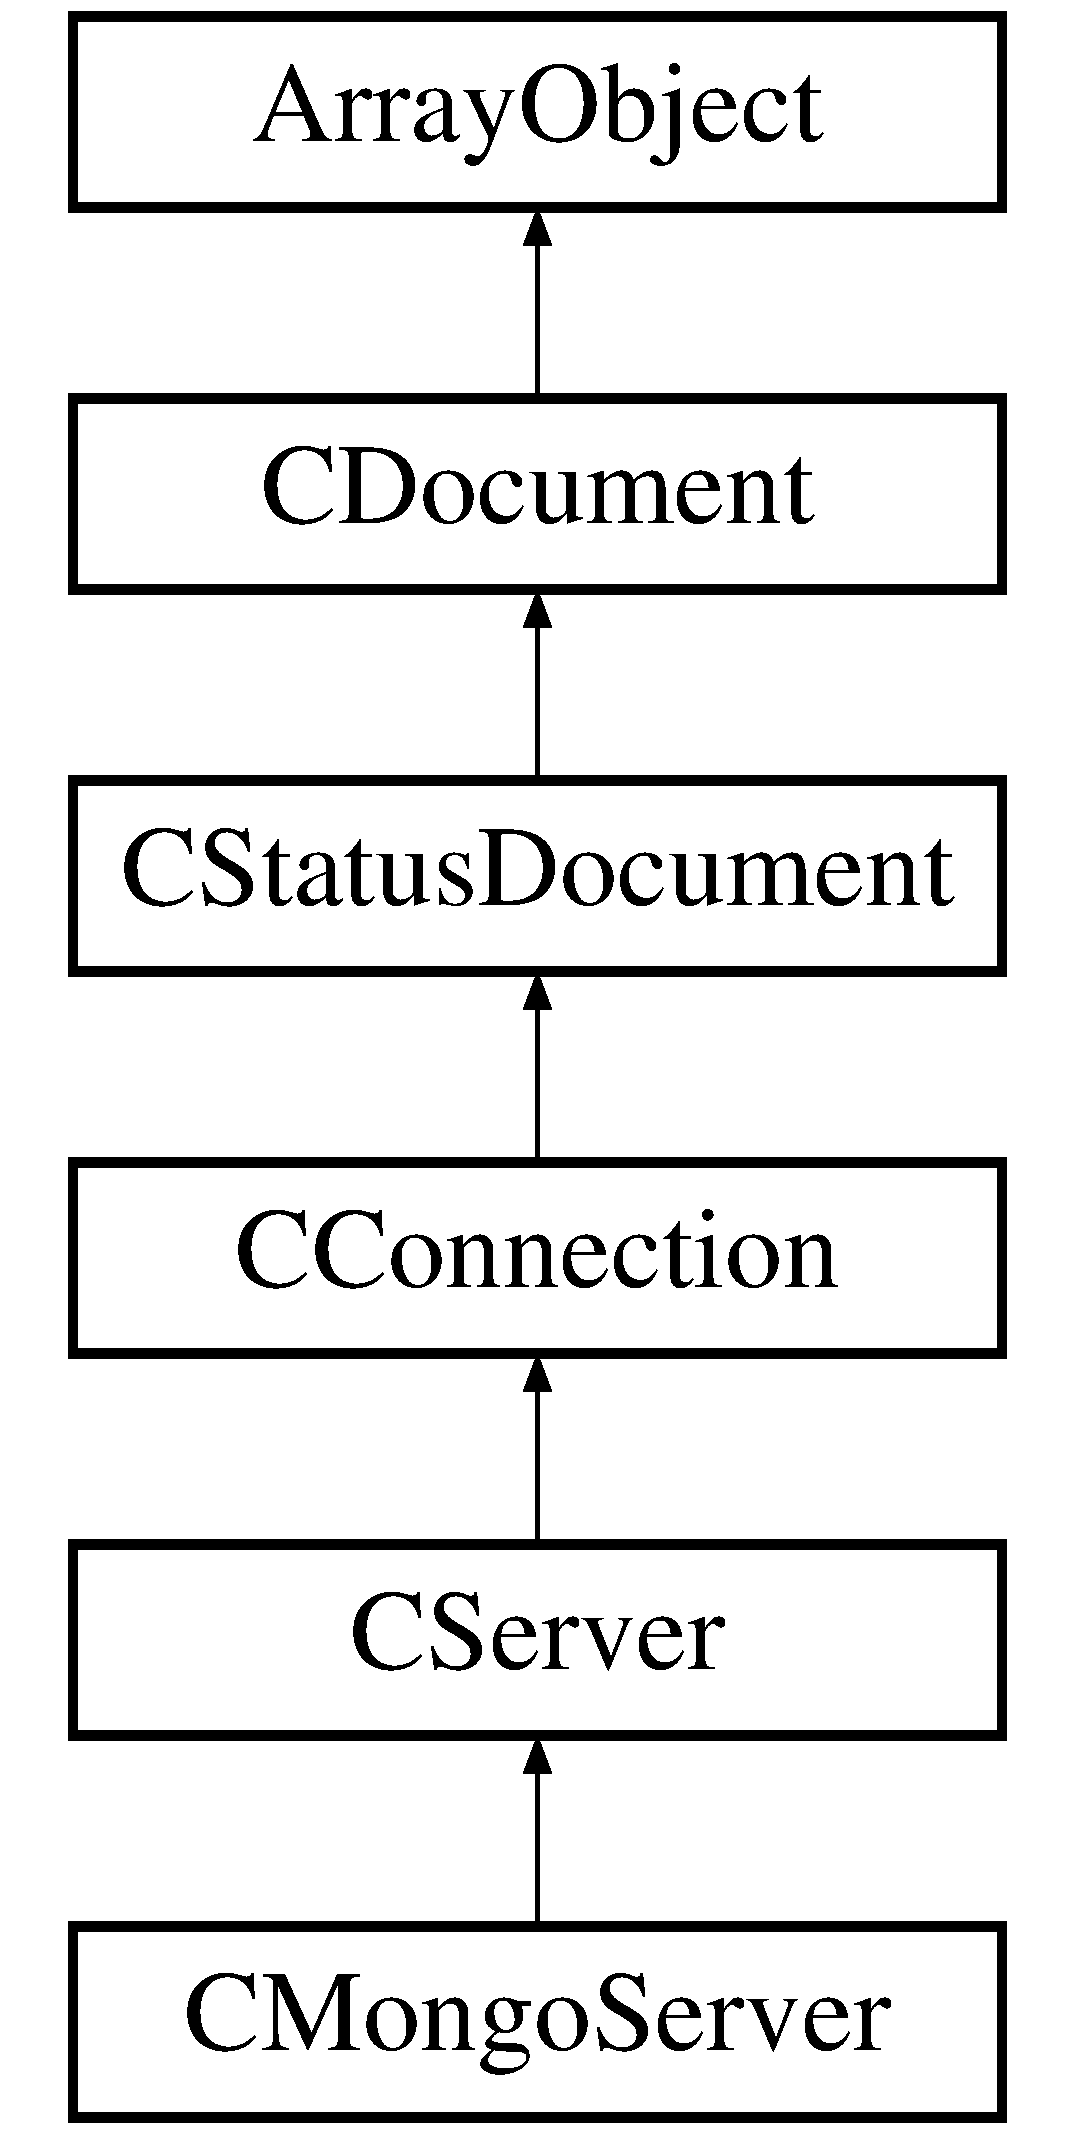
\includegraphics[height=6.000000cm]{class_c_server}
\end{center}
\end{figure}
\subsection*{Public Member Functions}
\begin{DoxyCompactItemize}
\item 
\hyperlink{class_c_server_abd12c8fabeb71e0400b21dc8cf93b9b1}{\-\_\-\-\_\-destruct} ()
\item 
\hyperlink{class_c_server_ac6e9bd058443274b3da40534d2fc741a}{Database} (\$the\-Database=N\-U\-L\-L)
\item 
\hyperlink{class_c_server_a23ace9fcb220408b293378051da8c084}{Graph} (\$the\-Value=N\-U\-L\-L, \$get\-Old=F\-A\-L\-S\-E)
\end{DoxyCompactItemize}
\subsection*{Protected Attributes}
\begin{DoxyCompactItemize}
\item 
\hypertarget{class_c_server_a7f59b9daedcaff19e284a38be45cd12d}{{\bfseries \$m\-Graph} = N\-U\-L\-L}\label{class_c_server_a7f59b9daedcaff19e284a38be45cd12d}

\end{DoxyCompactItemize}
\subsection*{Additional Inherited Members}


\subsection{Constructor \& Destructor Documentation}
\hypertarget{class_c_server_abd12c8fabeb71e0400b21dc8cf93b9b1}{\index{C\-Server@{C\-Server}!\-\_\-\-\_\-destruct@{\-\_\-\-\_\-destruct}}
\index{\-\_\-\-\_\-destruct@{\-\_\-\-\_\-destruct}!CServer@{C\-Server}}
\subsubsection[{\-\_\-\-\_\-destruct}]{\setlength{\rightskip}{0pt plus 5cm}C\-Server\-::\-\_\-\-\_\-destruct (
\begin{DoxyParamCaption}
{}
\end{DoxyParamCaption}
)}}\label{class_c_server_abd12c8fabeb71e0400b21dc8cf93b9b1}
\subparagraph*{Destructor}

We implement the destructor to get rid of the graph\-: the Neo4j P\-H\-P interface, for instance, has closures that cannot be serialised, so we need to reset the graph before destroying the object.

public 

\subsection{Member Function Documentation}
\hypertarget{class_c_server_ac6e9bd058443274b3da40534d2fc741a}{\index{C\-Server@{C\-Server}!Database@{Database}}
\index{Database@{Database}!CServer@{C\-Server}}
\subsubsection[{Database}]{\setlength{\rightskip}{0pt plus 5cm}C\-Server\-::\-Database (
\begin{DoxyParamCaption}
\item[{}]{\$the\-Database = {\ttfamily NULL}}
\end{DoxyParamCaption}
)\hspace{0.3cm}{\ttfamily [abstract]}}}\label{class_c_server_ac6e9bd058443274b3da40534d2fc741a}
\subparagraph*{Generate a database object}

This method can be used to return a database object belonging to the current server.

The parameter will be used by concrete instances to select which database to return, the goal of this class is only to declare the public interface, which must be implemented by specialised derived classes.

{\itshape Note\-: This method should also take care of setting the \hyperlink{}{k\-O\-F\-F\-S\-E\-T\-\_\-\-N\-A\-M\-E}, \hyperlink{}{k\-O\-F\-F\-S\-E\-T\-\_\-\-G\-R\-A\-P\-H} and \hyperlink{}{k\-O\-F\-F\-S\-E\-T\-\_\-\-P\-A\-R\-E\-N\-T} offsets of the generated object.}


\begin{DoxyParams}[1]{Parameters}
mixed & {\em \$the\-Database} & Database selector.\\
\hline
\end{DoxyParams}
public \begin{DoxyReturn}{Returns}
mixed The database object.
\end{DoxyReturn}
\begin{DoxySeeAlso}{See Also}
k\-O\-F\-F\-S\-E\-T\-\_\-\-N\-A\-M\-E k\-O\-F\-F\-S\-E\-T\-\_\-\-G\-R\-A\-P\-H k\-O\-F\-F\-S\-E\-T\-\_\-\-P\-A\-R\-E\-N\-T 
\end{DoxySeeAlso}
\hypertarget{class_c_server_a23ace9fcb220408b293378051da8c084}{\index{C\-Server@{C\-Server}!Graph@{Graph}}
\index{Graph@{Graph}!CServer@{C\-Server}}
\subsubsection[{Graph}]{\setlength{\rightskip}{0pt plus 5cm}C\-Server\-::\-Graph (
\begin{DoxyParamCaption}
\item[{}]{\$the\-Value = {\ttfamily NULL}, }
\item[{}]{\$get\-Old = {\ttfamily FALSE}}
\end{DoxyParamCaption}
)}}\label{class_c_server_a23ace9fcb220408b293378051da8c084}
\subparagraph*{Set, retrieve or delete a graph container instance}

The first parameter can take the following values\-:


\begin{DoxyItemize}
\item {\ttfamily N\-U\-L\-L}\-: Return the current value. 
\item {\ttfamily F\-A\-L\-S\-E}\-: Delete the current value. 
\item {\itshape \hyperlink{class_c_graph_container}{C\-Graph\-Container}}\-: Set the value with the provided parameter. 
\end{DoxyItemize}

The second parameter is a boolean which if {\ttfamily T\-R\-U\-E} will return the {\itshape old} value when replacing containers; if {\ttfamily F\-A\-L\-S\-E}, it will return the currently set value.

{\itshape Note\-: If you generate databases from the server and containers from these databases, the graph will be passed on to those objects\-: if you afterwards change the graph, this will not be reflected in those objects.}


\begin{DoxyParams}[1]{Parameters}
\hyperlink{class_c_graph_container}{C\-Graph\-Container} & {\em \$the\-Value} & Graph container.\\
\hline
\end{DoxyParams}
public \begin{DoxyReturn}{Returns}
mixed {\itshape New} or {\itshape old} graph container.
\end{DoxyReturn}
Manage\-Property() 

The documentation for this class was generated from the following file\-:\begin{DoxyCompactItemize}
\item 
/\-Library/\-Web\-Server/\-Library/\-P\-H\-P\-Wrapper/classes/C\-Server.\-php\end{DoxyCompactItemize}

\hypertarget{class_c_status_document}{\section{C\-Status\-Document Class Reference}
\label{class_c_status_document}\index{C\-Status\-Document@{C\-Status\-Document}}
}
Inheritance diagram for C\-Status\-Document\-:\begin{figure}[H]
\begin{center}
\leavevmode
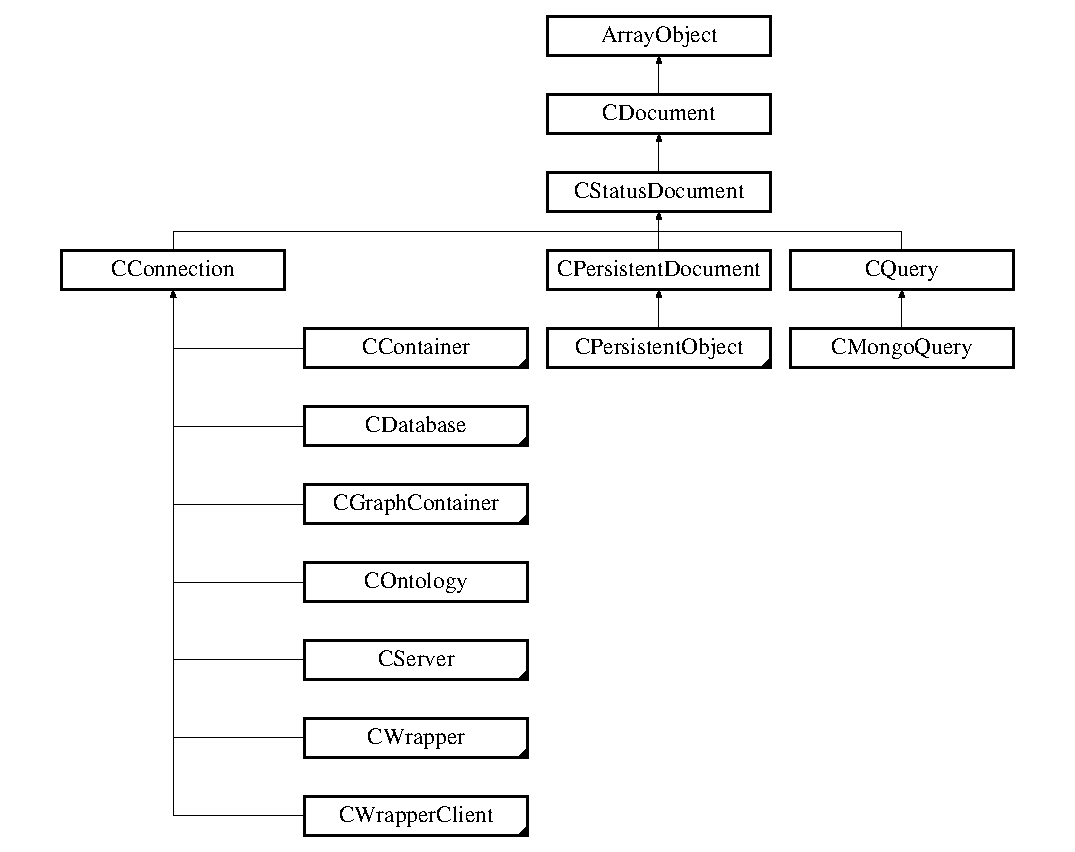
\includegraphics[height=11.000000cm]{class_c_status_document}
\end{center}
\end{figure}
\subsection*{Public Member Functions}
\begin{DoxyCompactItemize}
\item 
\hyperlink{class_c_status_document_a467c5b8ae2c40413cc918c69027bd43f}{\-\_\-\-\_\-construct} (\$the\-Input=Array(), \$the\-Flags=0, \$the\-Iterator= 'Array\-Iterator')
\item 
\hyperlink{class_c_status_document_a5c9a849e62516905de7a310960015a4b}{offset\-Set} (\$the\-Offset, \$the\-Value)
\item 
\hyperlink{class_c_status_document_afcc308cc116245a8c5a2eccc7fc2b1f1}{offset\-Unset} (\$the\-Offset)
\end{DoxyCompactItemize}
\subsection*{Protected Member Functions}
\begin{DoxyCompactItemize}
\item 
\hyperlink{class_c_status_document_a954dee06e219e0a0f2e7fa6edac56e28}{\-\_\-\-Is\-Inited} (\$the\-State=N\-U\-L\-L)
\item 
\hyperlink{class_c_status_document_ad5193995e1bff6de09acf3248a232ef9}{\-\_\-\-Is\-Dirty} (\$the\-State=N\-U\-L\-L)
\item 
\hyperlink{class_c_status_document_ab7d96fd4588cf7d5432fc65a1d1fb076}{\-\_\-\-Is\-Committed} (\$the\-State=N\-U\-L\-L)
\item 
\hyperlink{class_c_status_document_a86074a4afbabd35729c10aa4a1d31a82}{\-\_\-\-Is\-Encoded} (\$the\-State=N\-U\-L\-L)
\item 
\hyperlink{class_c_status_document_aceabdbc06743c524cf3c60d20b7f1fd7}{\-\_\-\-Ready} ()
\item 
\hyperlink{class_c_status_document_a51cac708e56c6c258f05c7458588ca47}{\-\_\-\-Preset} (\&\$the\-Offset, \&\$the\-Value)
\item 
\hyperlink{class_c_status_document_aa1d190aacd1573a699b572aae251e479}{\-\_\-\-Postset} (\&\$the\-Offset, \&\$the\-Value)
\item 
\hyperlink{class_c_status_document_a9507e9159eb7fc1b2a0965d1fd267fa8}{\-\_\-\-Preunset} (\&\$the\-Offset)
\item 
\hyperlink{class_c_status_document_a0022e449834b628db7f5f75698adb57d}{\-\_\-\-Postunset} (\&\$the\-Offset)
\end{DoxyCompactItemize}
\subsection*{Protected Attributes}
\begin{DoxyCompactItemize}
\item 
\hypertarget{class_c_status_document_a629582fbcf551372e99b06d79e78c9f1}{{\bfseries \$m\-Status} = k\-F\-L\-A\-G\-\_\-\-D\-E\-F\-A\-U\-L\-T}\label{class_c_status_document_a629582fbcf551372e99b06d79e78c9f1}

\end{DoxyCompactItemize}


\subsection{Constructor \& Destructor Documentation}
\hypertarget{class_c_status_document_a467c5b8ae2c40413cc918c69027bd43f}{\index{C\-Status\-Document@{C\-Status\-Document}!\-\_\-\-\_\-construct@{\-\_\-\-\_\-construct}}
\index{\-\_\-\-\_\-construct@{\-\_\-\-\_\-construct}!CStatusDocument@{C\-Status\-Document}}
\subsubsection[{\-\_\-\-\_\-construct}]{\setlength{\rightskip}{0pt plus 5cm}C\-Status\-Document\-::\-\_\-\-\_\-construct (
\begin{DoxyParamCaption}
\item[{}]{\$the\-Input = {\ttfamily Array()}, }
\item[{}]{\$the\-Flags = {\ttfamily 0}, }
\item[{}]{\$the\-Iterator = {\ttfamily 'ArrayIterator'}}
\end{DoxyParamCaption}
)}}\label{class_c_status_document_a467c5b8ae2c40413cc918c69027bd43f}
\subparagraph*{Instantiate class}

We overload the inherited constructor to set the \hyperlink{class_c_status_document_a954dee06e219e0a0f2e7fa6edac56e28}{\-\_\-\-Is\-Inited()} status.

This constructor mirrors the \hyperlink{}{Array\-Object} constructor.


\begin{DoxyParams}[1]{Parameters}
mixed & {\em \$the\-Input} & Input parameter. \\
\hline
integer & {\em \$the\-Flags} & Control flags. \\
\hline
string & {\em \$the\-Iterator} & Control flags.\\
\hline
\end{DoxyParams}
public

\hyperlink{class_c_status_document_aceabdbc06743c524cf3c60d20b7f1fd7}{\-\_\-\-Ready()}  \hyperlink{class_c_status_document_a954dee06e219e0a0f2e7fa6edac56e28}{\-\_\-\-Is\-Inited()} 

\subsection{Member Function Documentation}
\hypertarget{class_c_status_document_ab7d96fd4588cf7d5432fc65a1d1fb076}{\index{C\-Status\-Document@{C\-Status\-Document}!\-\_\-\-Is\-Committed@{\-\_\-\-Is\-Committed}}
\index{\-\_\-\-Is\-Committed@{\-\_\-\-Is\-Committed}!CStatusDocument@{C\-Status\-Document}}
\subsubsection[{\-\_\-\-Is\-Committed}]{\setlength{\rightskip}{0pt plus 5cm}C\-Status\-Document\-::\-\_\-\-Is\-Committed (
\begin{DoxyParamCaption}
\item[{}]{\$the\-State = {\ttfamily NULL}}
\end{DoxyParamCaption}
)\hspace{0.3cm}{\ttfamily [protected]}}}\label{class_c_status_document_ab7d96fd4588cf7d5432fc65a1d1fb076}
\subparagraph*{Manage committed status}

This method can be used to get or set the object's committed state.

A committed object is one that has either been loaded from a container or committed to a container, this state can be used in conjunction with the \hyperlink{}{k\-F\-L\-A\-G\-\_\-\-S\-T\-A\-T\-E\-\_\-\-D\-I\-R\-T\-Y} flag to determine whether an object needs to be committed.

The method features a single parameter\-:


\begin{DoxyItemize}
\item {\ttfamily N\-U\-L\-L}\-: The method will return the object's committed state. 
\item {\ttfamily T\-R\-U\-E}\-: The method will set the object's committed state. 
\item {\ttfamily F\-A\-L\-S\-E}\-: The method will reset the object's committed state. 
\end{DoxyItemize}

In all cases the method will return the state {\itshape after} it was eventually modified.


\begin{DoxyParams}[1]{Parameters}
mixed & {\em \$the\-State} & {\ttfamily T\-R\-U\-E}, {\ttfamily F\-A\-L\-S\-E} or {\ttfamily N\-U\-L\-L}.\\
\hline
\end{DoxyParams}
protected \begin{DoxyReturn}{Returns}
boolean {\ttfamily T\-R\-U\-E} committed, {\ttfamily F\-A\-L\-S\-E} uncommitted.
\end{DoxyReturn}
Manage\-Bit\-Field()

\begin{DoxySeeAlso}{See Also}
k\-F\-L\-A\-G\-\_\-\-S\-T\-A\-T\-E\-\_\-\-C\-O\-M\-M\-I\-T\-T\-E\-D 
\end{DoxySeeAlso}
\hypertarget{class_c_status_document_ad5193995e1bff6de09acf3248a232ef9}{\index{C\-Status\-Document@{C\-Status\-Document}!\-\_\-\-Is\-Dirty@{\-\_\-\-Is\-Dirty}}
\index{\-\_\-\-Is\-Dirty@{\-\_\-\-Is\-Dirty}!CStatusDocument@{C\-Status\-Document}}
\subsubsection[{\-\_\-\-Is\-Dirty}]{\setlength{\rightskip}{0pt plus 5cm}C\-Status\-Document\-::\-\_\-\-Is\-Dirty (
\begin{DoxyParamCaption}
\item[{}]{\$the\-State = {\ttfamily NULL}}
\end{DoxyParamCaption}
)\hspace{0.3cm}{\ttfamily [protected]}}}\label{class_c_status_document_ad5193995e1bff6de09acf3248a232ef9}
\subparagraph*{Manage dirty status}

This method can be used to get or set the object's dirty state.

A dirty object is one that was modified since the last time this state was probed. In general, this state should be set whenever the persistent properties of the object are modified.

In this class we automatically set this state when setting or unsetting offsets.

The method features a single parameter\-:


\begin{DoxyItemize}
\item {\ttfamily N\-U\-L\-L}\-: The method will return the object's dirty state. 
\item {\ttfamily T\-R\-U\-E}\-: The method will set the object's dirty state. 
\item {\ttfamily F\-A\-L\-S\-E}\-: The method will reset the object's dirty state. 
\end{DoxyItemize}

In all cases the method will return the state {\itshape after} it was eventually modified.


\begin{DoxyParams}[1]{Parameters}
mixed & {\em \$the\-State} & {\ttfamily T\-R\-U\-E}, {\ttfamily F\-A\-L\-S\-E} or {\ttfamily N\-U\-L\-L}.\\
\hline
\end{DoxyParams}
protected \begin{DoxyReturn}{Returns}
boolean {\ttfamily T\-R\-U\-E} dirty, {\ttfamily F\-A\-L\-S\-E} clean.
\end{DoxyReturn}
Manage\-Bit\-Field()

\begin{DoxySeeAlso}{See Also}
k\-F\-L\-A\-G\-\_\-\-S\-T\-A\-T\-E\-\_\-\-D\-I\-R\-T\-Y 
\end{DoxySeeAlso}
\hypertarget{class_c_status_document_a86074a4afbabd35729c10aa4a1d31a82}{\index{C\-Status\-Document@{C\-Status\-Document}!\-\_\-\-Is\-Encoded@{\-\_\-\-Is\-Encoded}}
\index{\-\_\-\-Is\-Encoded@{\-\_\-\-Is\-Encoded}!CStatusDocument@{C\-Status\-Document}}
\subsubsection[{\-\_\-\-Is\-Encoded}]{\setlength{\rightskip}{0pt plus 5cm}C\-Status\-Document\-::\-\_\-\-Is\-Encoded (
\begin{DoxyParamCaption}
\item[{}]{\$the\-State = {\ttfamily NULL}}
\end{DoxyParamCaption}
)\hspace{0.3cm}{\ttfamily [protected]}}}\label{class_c_status_document_a86074a4afbabd35729c10aa4a1d31a82}
\subparagraph*{Manage encoded status}

This method can be used to get or set the object's encoded state.

This flag determines whether the object should take care of serialising custom data types before the object is transmitted over the network.

The method features a single parameter\-:


\begin{DoxyItemize}
\item {\ttfamily N\-U\-L\-L}\-: The method will return the object's encoded state. 
\item {\ttfamily T\-R\-U\-E}\-: The method will set the object's encoded state. 
\item {\ttfamily F\-A\-L\-S\-E}\-: The method will reset the object's encoded state. 
\end{DoxyItemize}

In all cases the method will return the state {\itshape after} it was eventually modified.


\begin{DoxyParams}[1]{Parameters}
mixed & {\em \$the\-State} & {\ttfamily T\-R\-U\-E}, {\ttfamily F\-A\-L\-S\-E} or {\ttfamily N\-U\-L\-L}.\\
\hline
\end{DoxyParams}
protected \begin{DoxyReturn}{Returns}
boolean {\ttfamily T\-R\-U\-E} supports encoding, {\ttfamily F\-A\-L\-S\-E} does not support encoding.
\end{DoxyReturn}
Manage\-Bit\-Field()

\begin{DoxySeeAlso}{See Also}
k\-F\-L\-A\-G\-\_\-\-S\-T\-A\-T\-E\-\_\-\-E\-N\-C\-O\-D\-E\-D 
\end{DoxySeeAlso}
\hypertarget{class_c_status_document_a954dee06e219e0a0f2e7fa6edac56e28}{\index{C\-Status\-Document@{C\-Status\-Document}!\-\_\-\-Is\-Inited@{\-\_\-\-Is\-Inited}}
\index{\-\_\-\-Is\-Inited@{\-\_\-\-Is\-Inited}!CStatusDocument@{C\-Status\-Document}}
\subsubsection[{\-\_\-\-Is\-Inited}]{\setlength{\rightskip}{0pt plus 5cm}C\-Status\-Document\-::\-\_\-\-Is\-Inited (
\begin{DoxyParamCaption}
\item[{}]{\$the\-State = {\ttfamily NULL}}
\end{DoxyParamCaption}
)\hspace{0.3cm}{\ttfamily [protected]}}}\label{class_c_status_document_a954dee06e219e0a0f2e7fa6edac56e28}
\subparagraph*{Manage inited status}

This method can be used to get or set the object's inited state.

An object becomes inited when it has all the required elements necessary for it to be correctly used or persistently stored. Such a state indicates that at least the minimum required information was initialised in the object.

The counterpart state indicates that the object still lacks the necessary elements to successfully operate the object.

This method operates by setting or clearing the \hyperlink{}{k\-F\-L\-A\-G\-\_\-\-S\-T\-A\-T\-E\-\_\-\-I\-N\-I\-T\-E\-D} flag.

The method features a single parameter\-:


\begin{DoxyItemize}
\item {\ttfamily N\-U\-L\-L}\-: The method will return the object's inited state. 
\item {\ttfamily T\-R\-U\-E}\-: The method will set the object's inited state. 
\item {\ttfamily F\-A\-L\-S\-E}\-: The method will reset the object's inited state. 
\end{DoxyItemize}

In all cases the method will return the state {\itshape after} it was eventually modified.


\begin{DoxyParams}[1]{Parameters}
mixed & {\em \$the\-State} & {\ttfamily T\-R\-U\-E}, {\ttfamily F\-A\-L\-S\-E} or {\ttfamily N\-U\-L\-L}.\\
\hline
\end{DoxyParams}
protected \begin{DoxyReturn}{Returns}
boolean {\ttfamily T\-R\-U\-E} inited, {\ttfamily F\-A\-L\-S\-E} idle.
\end{DoxyReturn}
Manage\-Bit\-Field()

\begin{DoxySeeAlso}{See Also}
k\-F\-L\-A\-G\-\_\-\-S\-T\-A\-T\-E\-\_\-\-I\-N\-I\-T\-E\-D 
\end{DoxySeeAlso}
\hypertarget{class_c_status_document_aa1d190aacd1573a699b572aae251e479}{\index{C\-Status\-Document@{C\-Status\-Document}!\-\_\-\-Postset@{\-\_\-\-Postset}}
\index{\-\_\-\-Postset@{\-\_\-\-Postset}!CStatusDocument@{C\-Status\-Document}}
\subsubsection[{\-\_\-\-Postset}]{\setlength{\rightskip}{0pt plus 5cm}C\-Status\-Document\-::\-\_\-\-Postset (
\begin{DoxyParamCaption}
\item[{\&}]{\$the\-Offset, }
\item[{\&}]{\$the\-Value}
\end{DoxyParamCaption}
)\hspace{0.3cm}{\ttfamily [protected]}}}\label{class_c_status_document_aa1d190aacd1573a699b572aae251e479}
\subparagraph*{Handle offset after setting it}

This method will be called after the offset is set into the object only if the provided value is not equivalent to the stored value, it gives the chance to normalise the value after it gets stored in the object.

The method accepts the same parameters as the \hyperlink{class_c_status_document_a5c9a849e62516905de7a310960015a4b}{offset\-Set()} method, except that they are passed by reference.

In this class we update the \hyperlink{class_c_status_document_a954dee06e219e0a0f2e7fa6edac56e28}{\-\_\-\-Is\-Inited()} status.


\begin{DoxyParams}[1]{Parameters}
reference & {\em \&\$the\-Offset} & Offset. \\
\hline
reference & {\em \&\$the\-Value} & Value to set at offset.\\
\hline
\end{DoxyParams}
protected

\hyperlink{class_c_status_document_a954dee06e219e0a0f2e7fa6edac56e28}{\-\_\-\-Is\-Inited()}  \hyperlink{class_c_status_document_aceabdbc06743c524cf3c60d20b7f1fd7}{\-\_\-\-Ready()} \hypertarget{class_c_status_document_a0022e449834b628db7f5f75698adb57d}{\index{C\-Status\-Document@{C\-Status\-Document}!\-\_\-\-Postunset@{\-\_\-\-Postunset}}
\index{\-\_\-\-Postunset@{\-\_\-\-Postunset}!CStatusDocument@{C\-Status\-Document}}
\subsubsection[{\-\_\-\-Postunset}]{\setlength{\rightskip}{0pt plus 5cm}C\-Status\-Document\-::\-\_\-\-Postunset (
\begin{DoxyParamCaption}
\item[{\&}]{\$the\-Offset}
\end{DoxyParamCaption}
)\hspace{0.3cm}{\ttfamily [protected]}}}\label{class_c_status_document_a0022e449834b628db7f5f75698adb57d}
\subparagraph*{Handle offset after unsetting it}

This method will be called after the offset is unset from the object only if the provided offset existed in the object, it gives the chance to perform custom actions after a removal.

The method accepts the same parameter as the \hyperlink{class_c_status_document_afcc308cc116245a8c5a2eccc7fc2b1f1}{offset\-Unset()} method, except that it passed by reference.

In this class we update the \hyperlink{class_c_status_document_a954dee06e219e0a0f2e7fa6edac56e28}{\-\_\-\-Is\-Inited()} status.


\begin{DoxyParams}[1]{Parameters}
reference & {\em \&\$the\-Offset} & Offset.\\
\hline
\end{DoxyParams}
protected

\hyperlink{class_c_status_document_a954dee06e219e0a0f2e7fa6edac56e28}{\-\_\-\-Is\-Inited()}  \hyperlink{class_c_status_document_aceabdbc06743c524cf3c60d20b7f1fd7}{\-\_\-\-Ready()} \hypertarget{class_c_status_document_a51cac708e56c6c258f05c7458588ca47}{\index{C\-Status\-Document@{C\-Status\-Document}!\-\_\-\-Preset@{\-\_\-\-Preset}}
\index{\-\_\-\-Preset@{\-\_\-\-Preset}!CStatusDocument@{C\-Status\-Document}}
\subsubsection[{\-\_\-\-Preset}]{\setlength{\rightskip}{0pt plus 5cm}C\-Status\-Document\-::\-\_\-\-Preset (
\begin{DoxyParamCaption}
\item[{\&}]{\$the\-Offset, }
\item[{\&}]{\$the\-Value}
\end{DoxyParamCaption}
)\hspace{0.3cm}{\ttfamily [protected]}}}\label{class_c_status_document_a51cac708e56c6c258f05c7458588ca47}
\subparagraph*{Handle offset before setting it}

This method will be called before the offset is set into the object only if the provided value is not equivalent to the stored value, it gives the chance to normalise the value and offset before it gets stored in the object.

The method accepts the same parameters as the \hyperlink{class_c_status_document_a5c9a849e62516905de7a310960015a4b}{offset\-Set()} method, except that they are passed by reference.

In this class we set the \hyperlink{class_c_status_document_ad5193995e1bff6de09acf3248a232ef9}{\-\_\-\-Is\-Dirty()} status.


\begin{DoxyParams}[1]{Parameters}
reference & {\em \&\$the\-Offset} & Offset. \\
\hline
reference & {\em \&\$the\-Value} & Value to set at offset.\\
\hline
\end{DoxyParams}
protected

\hyperlink{class_c_status_document_ad5193995e1bff6de09acf3248a232ef9}{\-\_\-\-Is\-Dirty()} \hypertarget{class_c_status_document_a9507e9159eb7fc1b2a0965d1fd267fa8}{\index{C\-Status\-Document@{C\-Status\-Document}!\-\_\-\-Preunset@{\-\_\-\-Preunset}}
\index{\-\_\-\-Preunset@{\-\_\-\-Preunset}!CStatusDocument@{C\-Status\-Document}}
\subsubsection[{\-\_\-\-Preunset}]{\setlength{\rightskip}{0pt plus 5cm}C\-Status\-Document\-::\-\_\-\-Preunset (
\begin{DoxyParamCaption}
\item[{\&}]{\$the\-Offset}
\end{DoxyParamCaption}
)\hspace{0.3cm}{\ttfamily [protected]}}}\label{class_c_status_document_a9507e9159eb7fc1b2a0965d1fd267fa8}
\subparagraph*{Handle offset before unsetting it}

This method will be called before the offset is unset from the object only if the provided offset exists in the object, it gives the chance to perform custom actions and change the provided offset.

The method accepts the same parameter as the \hyperlink{class_c_status_document_afcc308cc116245a8c5a2eccc7fc2b1f1}{offset\-Unset()} method, except that it passed by reference.

In this class we set the \hyperlink{class_c_status_document_ad5193995e1bff6de09acf3248a232ef9}{\-\_\-\-Is\-Dirty()} status.


\begin{DoxyParams}[1]{Parameters}
reference & {\em \&\$the\-Offset} & Offset.\\
\hline
\end{DoxyParams}
protected

\hyperlink{class_c_status_document_ad5193995e1bff6de09acf3248a232ef9}{\-\_\-\-Is\-Dirty()} \hypertarget{class_c_status_document_aceabdbc06743c524cf3c60d20b7f1fd7}{\index{C\-Status\-Document@{C\-Status\-Document}!\-\_\-\-Ready@{\-\_\-\-Ready}}
\index{\-\_\-\-Ready@{\-\_\-\-Ready}!CStatusDocument@{C\-Status\-Document}}
\subsubsection[{\-\_\-\-Ready}]{\setlength{\rightskip}{0pt plus 5cm}C\-Status\-Document\-::\-\_\-\-Ready (
\begin{DoxyParamCaption}
{}
\end{DoxyParamCaption}
)\hspace{0.3cm}{\ttfamily [protected]}}}\label{class_c_status_document_aceabdbc06743c524cf3c60d20b7f1fd7}
\subparagraph*{Determine if the object is ready}

This method will return a boolean indicating whether all the required the elements managed by the current class are present, this value should then be set by the caller into the \hyperlink{class_c_status_document_a954dee06e219e0a0f2e7fa6edac56e28}{\-\_\-\-Is\-Inited()} status.

This method should be implemented in all inheritance levels in which the \hyperlink{class_c_status_document_a954dee06e219e0a0f2e7fa6edac56e28}{\} status is affected, it is the place where one may concentrate all the necessary tests to determine whether the object is usable. In this class we assume the object is  \-\_\-\-Is\-Inited()\}, it is up to derived classes to prove the contrary.  protected  boolean {\ttfamily T\-R\-U\-E} means  \-\_\-\-Is\-Inited( {\ttfamily T\-R\-U\-E} ). }\hypertarget{class_c_status_document_a5c9a849e62516905de7a310960015a4b}{\index{C\-Status\-Document@{C\-Status\-Document}!offset\-Set@{offset\-Set}}
\index{offset\-Set@{offset\-Set}!CStatusDocument@{C\-Status\-Document}}
\subsubsection[{offset\-Set}]{\setlength{\rightskip}{0pt plus 5cm}C\-Status\-Document\-::offset\-Set (
\begin{DoxyParamCaption}
\item[{}]{\$the\-Offset, }
\item[{}]{\$the\-Value}
\end{DoxyParamCaption}
)}}\label{class_c_status_document_a5c9a849e62516905de7a310960015a4b}
\subparagraph*{Set a value for a given offset}

We override this method to handle the dirty flag\-: when the value changes, we turn the \hyperlink{class_c_status_document_ad5193995e1bff6de09acf3248a232ef9}{\-\_\-\-Is\-Dirty()} status flag on.


\begin{DoxyParams}[1]{Parameters}
string & {\em \$the\-Offset} & Offset. \\
\hline
mixed & {\em \$the\-Value} & Value to set at offset.\\
\hline
\end{DoxyParams}
public

\hyperlink{class_c_status_document_a51cac708e56c6c258f05c7458588ca47}{\-\_\-\-Preset()}  \hyperlink{class_c_status_document_aa1d190aacd1573a699b572aae251e479}{\-\_\-\-Postset()} \hypertarget{class_c_status_document_afcc308cc116245a8c5a2eccc7fc2b1f1}{\index{C\-Status\-Document@{C\-Status\-Document}!offset\-Unset@{offset\-Unset}}
\index{offset\-Unset@{offset\-Unset}!CStatusDocument@{C\-Status\-Document}}
\subsubsection[{offset\-Unset}]{\setlength{\rightskip}{0pt plus 5cm}C\-Status\-Document\-::offset\-Unset (
\begin{DoxyParamCaption}
\item[{}]{\$the\-Offset}
\end{DoxyParamCaption}
)}}\label{class_c_status_document_afcc308cc116245a8c5a2eccc7fc2b1f1}
\subparagraph*{Reset a value for a given offset}

We override this method to handle the dirty flag\-: when the value changes, we turn the \hyperlink{class_c_status_document_ad5193995e1bff6de09acf3248a232ef9}{\-\_\-\-Is\-Dirty()} status flag on.


\begin{DoxyParams}[1]{Parameters}
string & {\em \$the\-Offset} & Offset.\\
\hline
\end{DoxyParams}
public

\hyperlink{class_c_status_document_a9507e9159eb7fc1b2a0965d1fd267fa8}{\-\_\-\-Preunset()}  \hyperlink{class_c_status_document_a0022e449834b628db7f5f75698adb57d}{\-\_\-\-Postunset()} 

The documentation for this class was generated from the following file\-:\begin{DoxyCompactItemize}
\item 
/\-Library/\-Web\-Server/\-Library/\-P\-H\-P\-Wrapper/classes/C\-Status\-Document.\-php\end{DoxyCompactItemize}

\hypertarget{class_c_tag}{\section{C\-Tag Class Reference}
\label{class_c_tag}\index{C\-Tag@{C\-Tag}}
}
Inheritance diagram for C\-Tag\-:\begin{figure}[H]
\begin{center}
\leavevmode
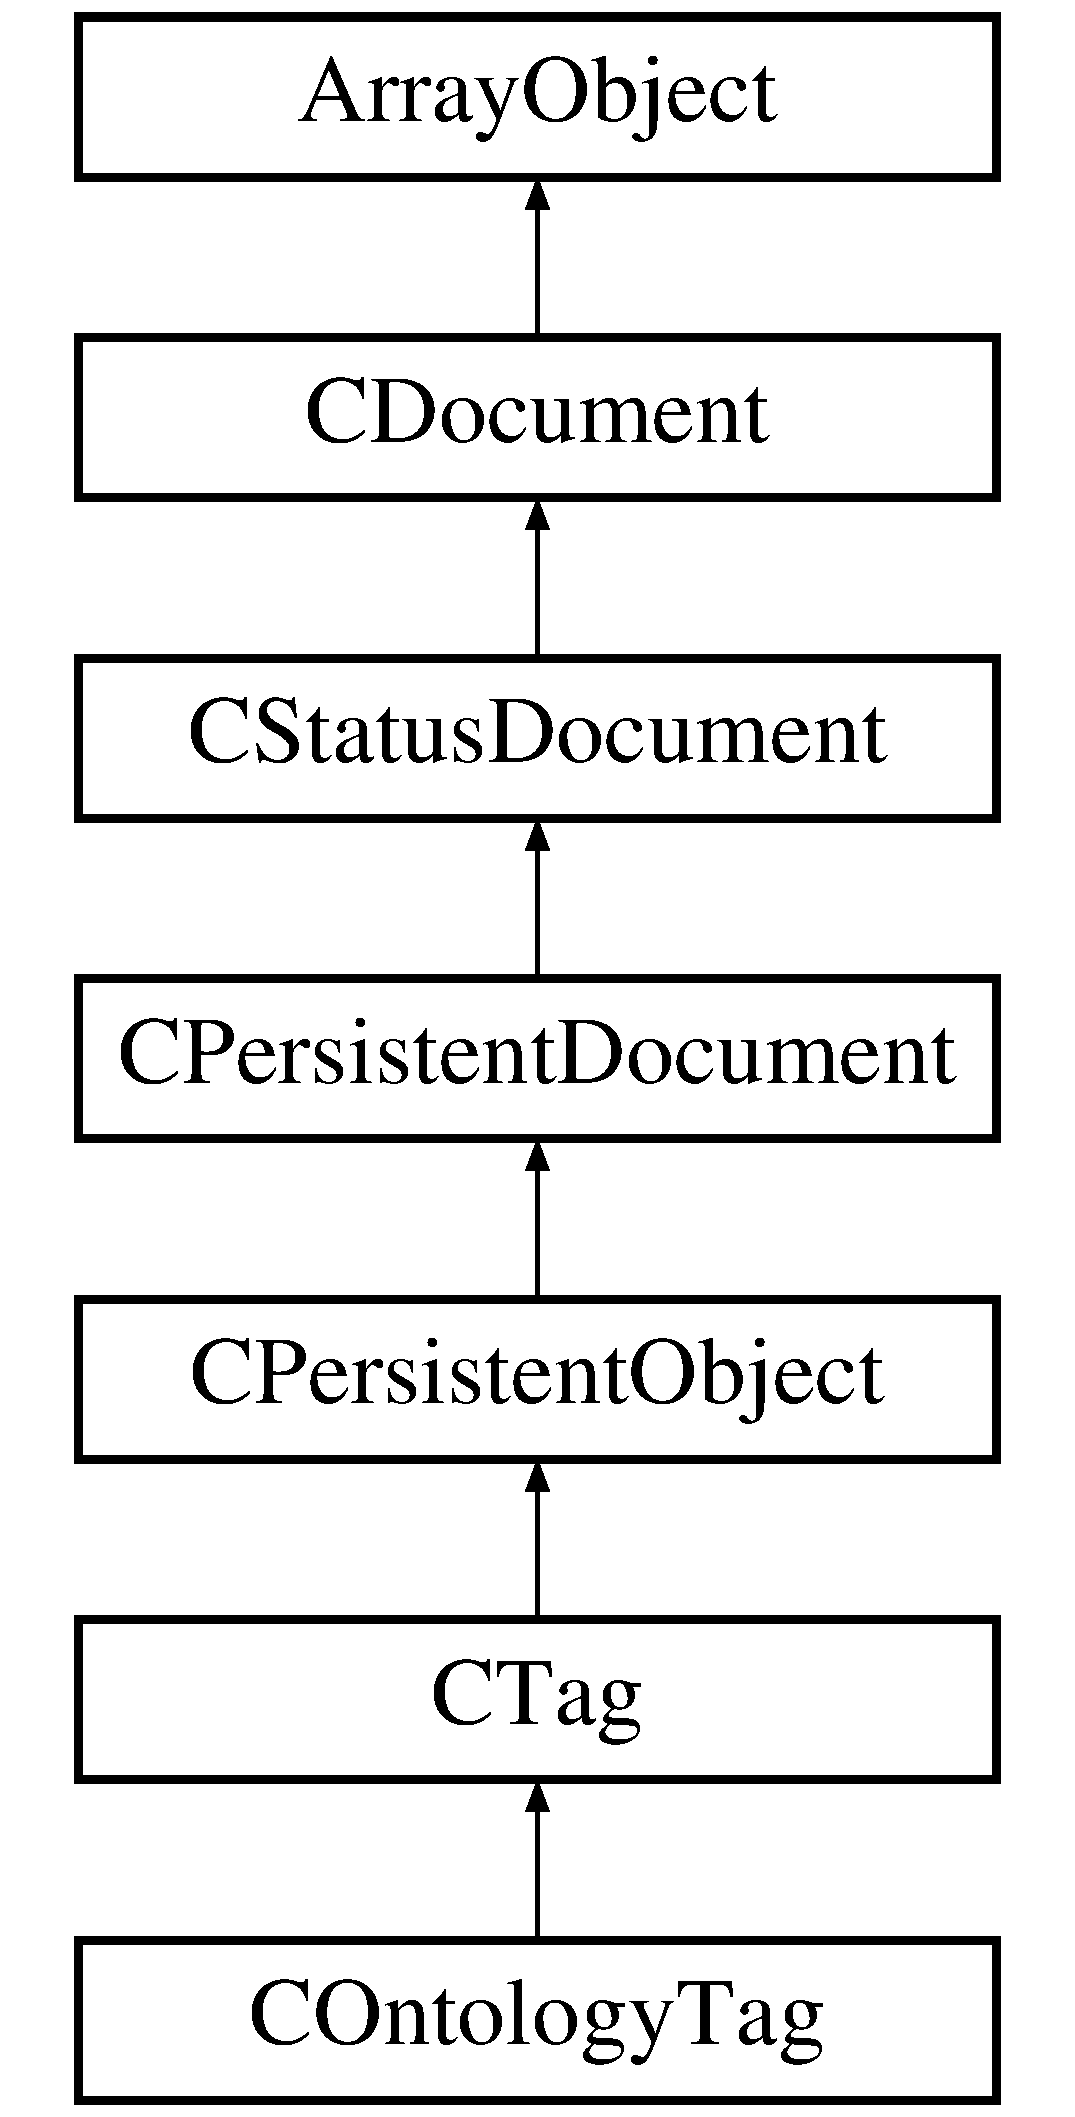
\includegraphics[height=7.000000cm]{class_c_tag}
\end{center}
\end{figure}
\subsection*{Public Member Functions}
\begin{DoxyCompactItemize}
\item 
\hyperlink{class_c_tag_a5bde38c2605d2559fd8d9c9d85904751}{Synonym} (\$the\-Value=N\-U\-L\-L, \$the\-Operation=N\-U\-L\-L, \$get\-Old=F\-A\-L\-S\-E)
\item 
\hyperlink{class_c_tag_a3ce611f613f6317f450354da2057b90c}{Push\-Item} (\$the\-Value)
\item 
\hyperlink{class_c_tag_a5df518ef6a881d7c2de469fef50ddd92}{Pop\-Item} ()
\end{DoxyCompactItemize}
\subsection*{Protected Member Functions}
\begin{DoxyCompactItemize}
\item 
\hyperlink{class_c_tag_a6797a73041d6d630799998fce617b404}{\-\_\-index} (\hyperlink{class_c_connection}{C\-Connection} \$the\-Connection, \$the\-Modifiers)
\item 
\hyperlink{class_c_tag_a486d3f1d1c789fe14f258ce008d5af5a}{\-\_\-\-Preset} (\&\$the\-Offset, \&\$the\-Value)
\item 
\hyperlink{class_c_tag_a5131b8768fa08bbcecb1c65a046e302c}{\-\_\-\-Preunset} (\&\$the\-Offset)
\item 
\hyperlink{class_c_tag_abc2d1e24a8fc606ff4d6dd018d5af42d}{\-\_\-\-Precommit\-Validate} (\&\$the\-Connection, \&\$the\-Modifiers)
\item 
\hyperlink{class_c_tag_a9fed7b05a04413e04c19a49e592e6242}{\-\_\-\-Ready} ()
\end{DoxyCompactItemize}
\subsection*{Additional Inherited Members}


\subsection{Member Function Documentation}
\hypertarget{class_c_tag_a6797a73041d6d630799998fce617b404}{\index{C\-Tag@{C\-Tag}!\-\_\-index@{\-\_\-index}}
\index{\-\_\-index@{\-\_\-index}!CTag@{C\-Tag}}
\subsubsection[{\-\_\-index}]{\setlength{\rightskip}{0pt plus 5cm}C\-Tag\-::\-\_\-index (
\begin{DoxyParamCaption}
\item[{{\bf C\-Connection}}]{\$the\-Connection, }
\item[{}]{\$the\-Modifiers}
\end{DoxyParamCaption}
)\hspace{0.3cm}{\ttfamily [protected]}}}\label{class_c_tag_a6797a73041d6d630799998fce617b404}
\subparagraph*{Return the object's global unique identifier}

The tag is identified by its path items, this method will return the list of items separated by the \hyperlink{}{k\-T\-O\-K\-E\-N\-\_\-\-I\-N\-D\-E\-X\-\_\-\-S\-E\-P\-A\-R\-A\-T\-O\-R} token.

This also means that all elements of the path must be convertable to string.


\begin{DoxyParams}[1]{Parameters}
\hyperlink{class_c_connection}{C\-Connection} & {\em \$the\-Connection} & Server, database or container. \\
\hline
bitfield & {\em \$the\-Modifiers} & Commit options.\\
\hline
\end{DoxyParams}
protected \begin{DoxyReturn}{Returns}
string$|$\-N\-U\-L\-L The object's global unique identifier.
\end{DoxyReturn}
\begin{DoxySeeAlso}{See Also}
k\-T\-A\-G\-\_\-\-P\-A\-T\-H k\-T\-O\-K\-E\-N\-\_\-\-I\-N\-D\-E\-X\-\_\-\-S\-E\-P\-A\-R\-A\-T\-O\-R 
\end{DoxySeeAlso}
\hypertarget{class_c_tag_abc2d1e24a8fc606ff4d6dd018d5af42d}{\index{C\-Tag@{C\-Tag}!\-\_\-\-Precommit\-Validate@{\-\_\-\-Precommit\-Validate}}
\index{\-\_\-\-Precommit\-Validate@{\-\_\-\-Precommit\-Validate}!CTag@{C\-Tag}}
\subsubsection[{\-\_\-\-Precommit\-Validate}]{\setlength{\rightskip}{0pt plus 5cm}C\-Tag\-::\-\_\-\-Precommit\-Validate (
\begin{DoxyParamCaption}
\item[{\&}]{\$the\-Connection, }
\item[{\&}]{\$the\-Modifiers}
\end{DoxyParamCaption}
)\hspace{0.3cm}{\ttfamily [protected]}}}\label{class_c_tag_abc2d1e24a8fc606ff4d6dd018d5af42d}
\subparagraph*{Validate the object before committing}

In this class we check if the current path has an odd number of items, if that is not the case, the method will raise an exception.


\begin{DoxyParams}[1]{Parameters}
reference & {\em \&\$the\-Connection} & Server, database or container. \\
\hline
reference & {\em \&\$the\-Modifiers} & Commit options.\\
\hline
\end{DoxyParams}
protected \begin{DoxyReturn}{Returns}
mixed
\end{DoxyReturn}

\begin{DoxyExceptions}{Exceptions}
{\em Exception} & \\
\hline
\end{DoxyExceptions}
\begin{DoxySeeAlso}{See Also}
k\-T\-A\-G\-\_\-\-P\-A\-T\-H 
\end{DoxySeeAlso}
\hypertarget{class_c_tag_a486d3f1d1c789fe14f258ce008d5af5a}{\index{C\-Tag@{C\-Tag}!\-\_\-\-Preset@{\-\_\-\-Preset}}
\index{\-\_\-\-Preset@{\-\_\-\-Preset}!CTag@{C\-Tag}}
\subsubsection[{\-\_\-\-Preset}]{\setlength{\rightskip}{0pt plus 5cm}C\-Tag\-::\-\_\-\-Preset (
\begin{DoxyParamCaption}
\item[{\&}]{\$the\-Offset, }
\item[{\&}]{\$the\-Value}
\end{DoxyParamCaption}
)\hspace{0.3cm}{\ttfamily [protected]}}}\label{class_c_tag_a486d3f1d1c789fe14f258ce008d5af5a}
\subparagraph*{Handle offset before setting it}

In this class we ensure that the \hyperlink{}{k\-T\-A\-G\-\_\-\-P\-A\-T\-H} offset is an array, Array\-Object instances are not counted as an array.

We also prevent changing the data type once the object was committed.


\begin{DoxyParams}[1]{Parameters}
reference & {\em \&\$the\-Offset} & Offset. \\
\hline
reference & {\em \&\$the\-Value} & Value to set at offset.\\
\hline
\end{DoxyParams}
protected


\begin{DoxyExceptions}{Exceptions}
{\em Exception} & \\
\hline
\end{DoxyExceptions}
\begin{DoxySeeAlso}{See Also}
k\-T\-A\-G\-\_\-\-P\-A\-T\-H 
\end{DoxySeeAlso}
\hypertarget{class_c_tag_a5131b8768fa08bbcecb1c65a046e302c}{\index{C\-Tag@{C\-Tag}!\-\_\-\-Preunset@{\-\_\-\-Preunset}}
\index{\-\_\-\-Preunset@{\-\_\-\-Preunset}!CTag@{C\-Tag}}
\subsubsection[{\-\_\-\-Preunset}]{\setlength{\rightskip}{0pt plus 5cm}C\-Tag\-::\-\_\-\-Preunset (
\begin{DoxyParamCaption}
\item[{\&}]{\$the\-Offset}
\end{DoxyParamCaption}
)\hspace{0.3cm}{\ttfamily [protected]}}}\label{class_c_tag_a5131b8768fa08bbcecb1c65a046e302c}
\subparagraph*{Handle offset before unsetting it}

In this class we prevent resetting the path and the data type once the object is committed.


\begin{DoxyParams}[1]{Parameters}
reference & {\em \&\$the\-Offset} & Offset.\\
\hline
\end{DoxyParams}
protected

\hyperlink{class_c_status_document_ad5193995e1bff6de09acf3248a232ef9}{\-\_\-\-Is\-Dirty()} \hypertarget{class_c_tag_a9fed7b05a04413e04c19a49e592e6242}{\index{C\-Tag@{C\-Tag}!\-\_\-\-Ready@{\-\_\-\-Ready}}
\index{\-\_\-\-Ready@{\-\_\-\-Ready}!CTag@{C\-Tag}}
\subsubsection[{\-\_\-\-Ready}]{\setlength{\rightskip}{0pt plus 5cm}C\-Tag\-::\-\_\-\-Ready (
\begin{DoxyParamCaption}
{}
\end{DoxyParamCaption}
)\hspace{0.3cm}{\ttfamily [protected]}}}\label{class_c_tag_a9fed7b05a04413e04c19a49e592e6242}
\subparagraph*{Determine if the object is ready}

In this class we tie the \hyperlink{class_c_status_document_a954dee06e219e0a0f2e7fa6edac56e28}{\-\_\-\-Is\-Inited()} status to the presence or absence of the \hyperlink{}{k\-T\-A\-G\-\_\-\-P\-A\-T\-H} offset.

protected \begin{DoxyReturn}{Returns}
boolean {\ttfamily T\-R\-U\-E} means \hyperlink{}{.  \-\_\-\-Ready()  k\-T\-A\-G\-\_\-\-P\-A\-T\-H }
\end{DoxyReturn}
\hypertarget{class_c_tag_a5df518ef6a881d7c2de469fef50ddd92}{\index{C\-Tag@{C\-Tag}!Pop\-Item@{Pop\-Item}}
\index{Pop\-Item@{Pop\-Item}!CTag@{C\-Tag}}
\subsubsection[{Pop\-Item}]{\setlength{\rightskip}{0pt plus 5cm}C\-Tag\-::\-Pop\-Item (
\begin{DoxyParamCaption}
{}
\end{DoxyParamCaption}
)}}\label{class_c_tag_a5df518ef6a881d7c2de469fef50ddd92}
\subparagraph*{Remove from path}

This method will remove the last item from the tag path and return it to the caller.

If the removed item is the last one, the offset will be deleted, if the list is missing, the method will return {\ttfamily N\-U\-L\-L}.

public \begin{DoxyReturn}{Returns}
mixed Last item of the list or {\ttfamily N\-U\-L\-L}.
\end{DoxyReturn}
\begin{DoxySeeAlso}{See Also}
k\-T\-A\-G\-\_\-\-P\-A\-T\-H 
\end{DoxySeeAlso}
\hypertarget{class_c_tag_a3ce611f613f6317f450354da2057b90c}{\index{C\-Tag@{C\-Tag}!Push\-Item@{Push\-Item}}
\index{Push\-Item@{Push\-Item}!CTag@{C\-Tag}}
\subsubsection[{Push\-Item}]{\setlength{\rightskip}{0pt plus 5cm}C\-Tag\-::\-Push\-Item (
\begin{DoxyParamCaption}
\item[{}]{\$the\-Value}
\end{DoxyParamCaption}
)}}\label{class_c_tag_a3ce611f613f6317f450354da2057b90c}
\subparagraph*{Append to path}

This method will add the provided item to the tag path, the element will be appended to the end of the list.

The provided item is considered as-\/is, that means that arrays are considered as a scalar item. If you provide {\ttfamily N\-U\-L\-L} as the value, this will be ignored and the method will return {\ttfamily F\-A\-L\-S\-E}.

The method will return the current number of items in the list.


\begin{DoxyParams}[1]{Parameters}
mixed & {\em \$the\-Value} & Value to append.\\
\hline
\end{DoxyParams}
public \begin{DoxyReturn}{Returns}
integer Number of items in the list.
\end{DoxyReturn}
\begin{DoxySeeAlso}{See Also}
k\-T\-A\-G\-\_\-\-P\-A\-T\-H 
\end{DoxySeeAlso}
\hypertarget{class_c_tag_a5bde38c2605d2559fd8d9c9d85904751}{\index{C\-Tag@{C\-Tag}!Synonym@{Synonym}}
\index{Synonym@{Synonym}!CTag@{C\-Tag}}
\subsubsection[{Synonym}]{\setlength{\rightskip}{0pt plus 5cm}C\-Tag\-::\-Synonym (
\begin{DoxyParamCaption}
\item[{}]{\$the\-Value = {\ttfamily NULL}, }
\item[{}]{\$the\-Operation = {\ttfamily NULL}, }
\item[{}]{\$get\-Old = {\ttfamily FALSE}}
\end{DoxyParamCaption}
)}}\label{class_c_tag_a5bde38c2605d2559fd8d9c9d85904751}
\subparagraph*{Manage tag synonyms}

This method can be used to manage the tag's synonyms, \hyperlink{}{k\-T\-A\-G\-\_\-\-S\-Y\-N\-O\-N\-Y\-M\-S}, which contains a list of strings that represent alternate codes or names that can be used to identify the tag.

This offset collects the list of synonyms in an enumerated set that can be managed with the following parameters\-:


\begin{DoxyItemize}
\item {\ttfamily \$the\-Value}\-: Depending on the next parameter, this may either refer to the value to be set or to the index of the element to be retrieved or deleted\-: 
\begin{DoxyItemize}
\item {\ttfamily N\-U\-L\-L}\-: This value indicates that we want to operate on all elements, which means, in practical terms, that we either want to retrieve or delete the full list. If the operation parameter resolves to {\ttfamily T\-R\-U\-E}, the method will default to retrieving the current list and no new element will be added. 
\item {\ttfamily array}\-: An array indicates that we want to operate on a list of values and that other parameters may also be provided as lists. Note that \hyperlink{}{Array\-Object} instances are not considered here as arrays. 
\item {\itshape other}\-: Any other type represents either the new value to be added or the index to the value to be returned or deleted. 
\end{DoxyItemize}
\item {\ttfamily \$the\-Operation}\-: This parameter represents the operation to be performed whose scope depends on the value of the previous parameter\-: 
\begin{DoxyItemize}
\item {\ttfamily N\-U\-L\-L}\-: Return the element or full list. 
\item {\ttfamily F\-A\-L\-S\-E}\-: Delete the element or full list. 
\item {\ttfamily array}\-: This type is only considered if the {\ttfamily \$the\-Value} parameter is provided as an array\-: the method will be called for each element of the {\ttfamily \$the\-Value} parameter matched with the corresponding element of this parameter, which also means that both both parameters must share the same count. 
\item {\itshape other}\-: Add the {\ttfamily \$the\-Value} value to the list. If you provided {\ttfamily N\-U\-L\-L} in the previous parameter, the operation will be reset to {\ttfamily N\-U\-L\-L}. 
\end{DoxyItemize}
\item {\ttfamily \$get\-Old}\-: Determines what the method will return\-: 
\begin{DoxyItemize}
\item {\ttfamily T\-R\-U\-E}\-: Return the value {\itshape before} it was eventually modified. 
\item {\ttfamily F\-A\-L\-S\-E}\-: Return the value {\itshape after} it was eventually modified. 
\end{DoxyItemize}
\end{DoxyItemize}


\begin{DoxyParams}[1]{Parameters}
mixed & {\em \$the\-Value} & Value or index. \\
\hline
mixed & {\em \$the\-Operation} & Operation. \\
\hline
boolean & {\em \$get\-Old} & T\-R\-U\-E get old value.\\
\hline
\end{DoxyParams}
public \begin{DoxyReturn}{Returns}
mixed {\itshape New} or {\itshape old} type.
\end{DoxyReturn}
Manage\-Object\-Set\-Offset()

\begin{DoxySeeAlso}{See Also}
k\-T\-A\-G\-\_\-\-S\-Y\-N\-O\-N\-Y\-M\-S 
\end{DoxySeeAlso}


The documentation for this class was generated from the following file\-:\begin{DoxyCompactItemize}
\item 
/\-Library/\-Web\-Server/\-Library/\-P\-H\-P\-Wrapper/classes/C\-Tag.\-php\end{DoxyCompactItemize}

\hypertarget{class_c_term}{\section{C\-Term Class Reference}
\label{class_c_term}\index{C\-Term@{C\-Term}}
}
Inheritance diagram for C\-Term\-:\begin{figure}[H]
\begin{center}
\leavevmode
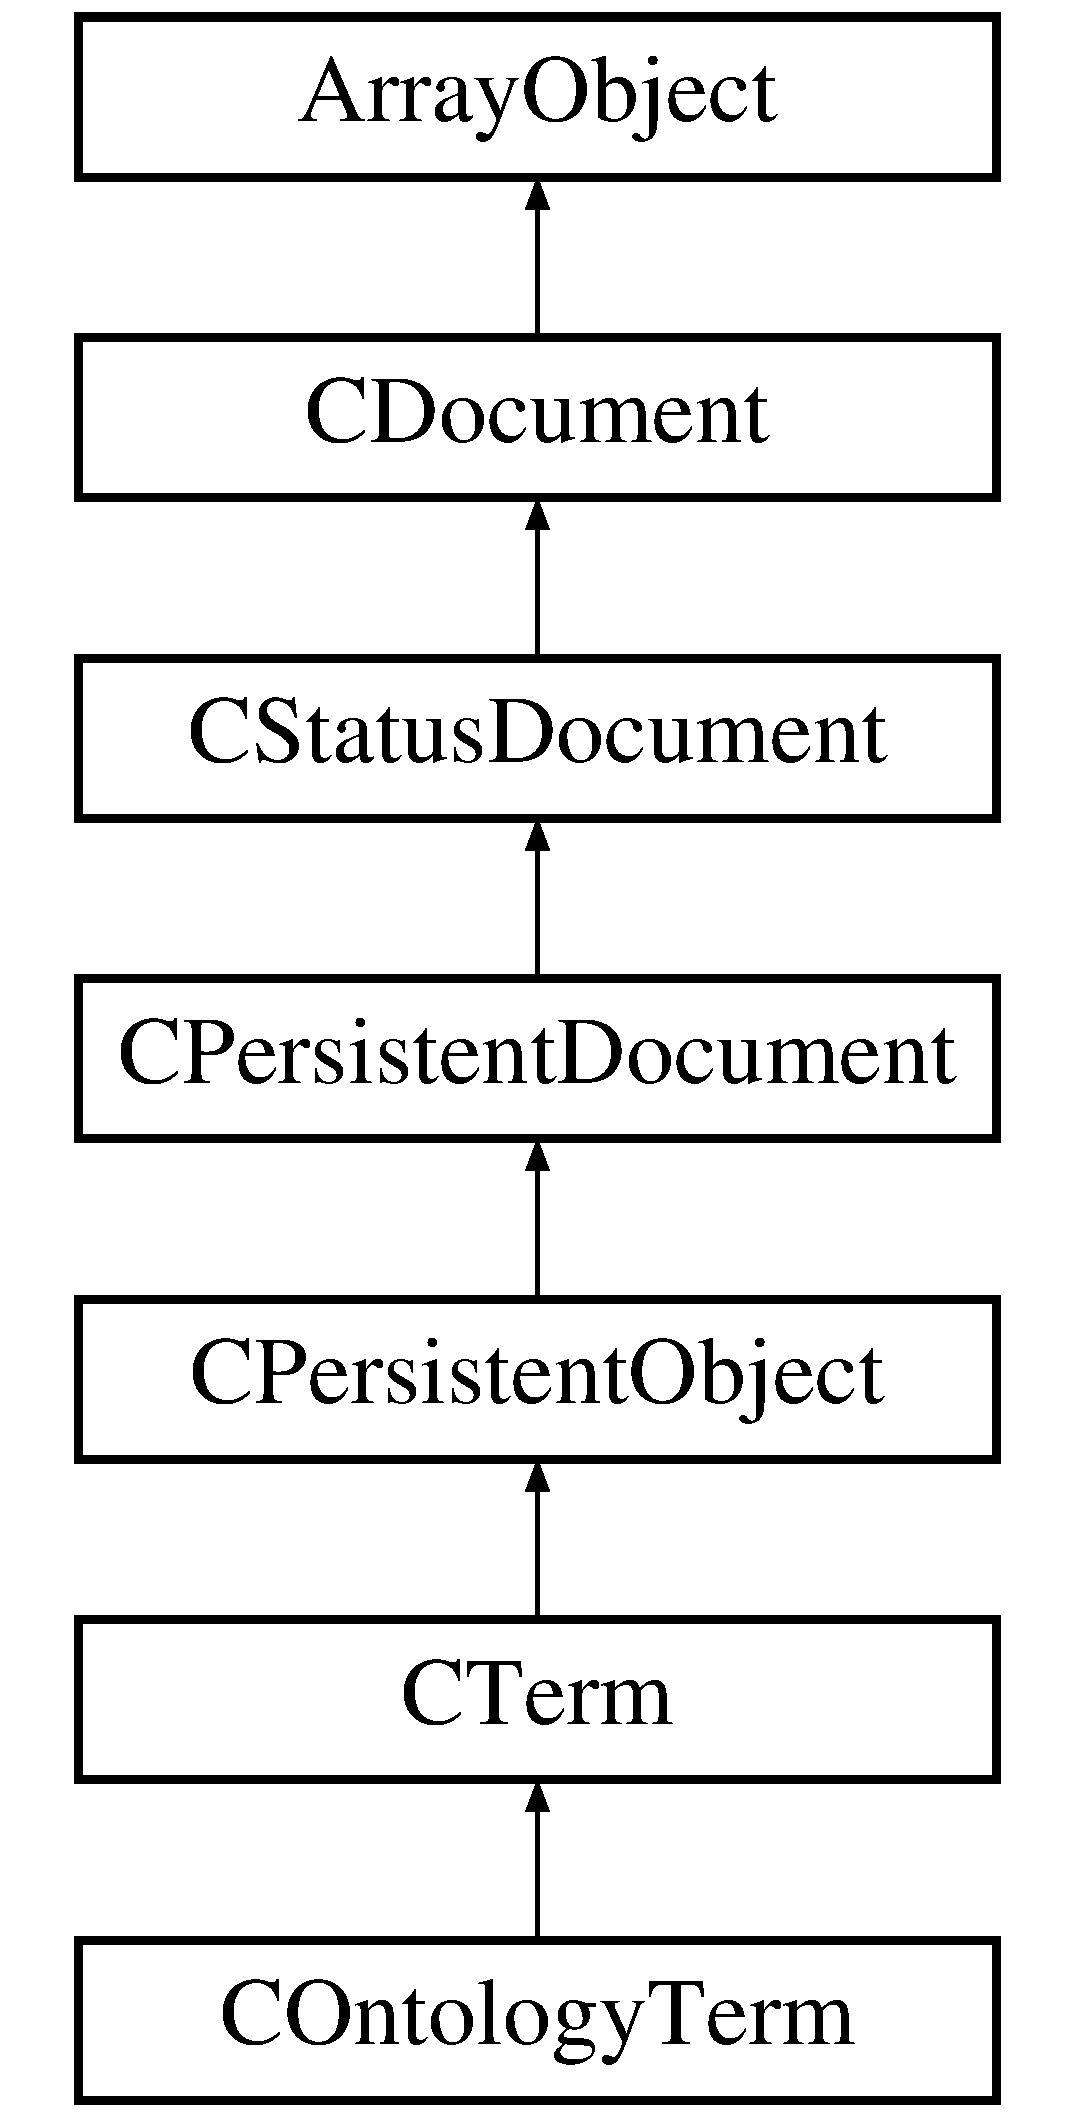
\includegraphics[height=7.000000cm]{class_c_term}
\end{center}
\end{figure}
\subsection*{Public Member Functions}
\begin{DoxyCompactItemize}
\item 
\hyperlink{class_c_term_a59a271c34a9f579bcf3177b392b6e31a}{N\-S} (\$the\-Value=N\-U\-L\-L, \$get\-Old=F\-A\-L\-S\-E)
\item 
\hyperlink{class_c_term_ae9a44c9e2b44ab35e28b6215a92ad0bf}{L\-I\-D} (\$the\-Value=N\-U\-L\-L, \$get\-Old=F\-A\-L\-S\-E)
\item 
\hyperlink{class_c_term_a4a8599bf7001354a6b4be80c73c11c9d}{Term} (\$the\-Value=N\-U\-L\-L, \$get\-Old=F\-A\-L\-S\-E)
\item 
\hyperlink{class_c_term_a6d832ed436e71f3c78411bd767dae182}{Label} (\$the\-Language=N\-U\-L\-L, \$the\-Value=N\-U\-L\-L, \$get\-Old=F\-A\-L\-S\-E)
\item 
\hyperlink{class_c_term_aa35db271304b2e8683ab1973c31d896f}{Definition} (\$the\-Language=N\-U\-L\-L, \$the\-Value=N\-U\-L\-L, \$get\-Old=F\-A\-L\-S\-E)
\item 
\hyperlink{class_c_term_acd2807647fc5af82bbcb02c797fde523}{Synonym} (\$the\-Value=N\-U\-L\-L, \$the\-Operation=N\-U\-L\-L, \$get\-Old=F\-A\-L\-S\-E)
\end{DoxyCompactItemize}
\subsection*{Static Public Member Functions}
\begin{DoxyCompactItemize}
\item 
static \hyperlink{class_c_term_a727ce4d7c7bb37d9e969456c03d2b1c0}{Term\-Code} (\$the\-Identifier, \$the\-Namespace=N\-U\-L\-L)
\end{DoxyCompactItemize}
\subsection*{Protected Member Functions}
\begin{DoxyCompactItemize}
\item 
\hyperlink{class_c_term_aa1d78e9ce7ece1a73e7244e1a9d2dbaf}{\-\_\-index} (\hyperlink{class_c_connection}{C\-Connection} \$the\-Connection, \$the\-Modifiers)
\item 
\hyperlink{class_c_term_aa4fea9e8e38ae888dd05142a6b8df097}{\-\_\-\-Preset} (\&\$the\-Offset, \&\$the\-Value)
\item 
\hyperlink{class_c_term_a0be6c6e9cc960f4df79f632d5b078ea0}{\-\_\-\-Preunset} (\&\$the\-Offset)
\item 
\hyperlink{class_c_term_a7a5f97930c2cc87d9f5a03dade1fb63c}{\-\_\-\-Ready} ()
\end{DoxyCompactItemize}
\subsection*{Additional Inherited Members}


\subsection{Member Function Documentation}
\hypertarget{class_c_term_aa1d78e9ce7ece1a73e7244e1a9d2dbaf}{\index{C\-Term@{C\-Term}!\-\_\-index@{\-\_\-index}}
\index{\-\_\-index@{\-\_\-index}!CTerm@{C\-Term}}
\subsubsection[{\-\_\-index}]{\setlength{\rightskip}{0pt plus 5cm}C\-Term\-::\-\_\-index (
\begin{DoxyParamCaption}
\item[{{\bf C\-Connection}}]{\$the\-Connection, }
\item[{}]{\$the\-Modifiers}
\end{DoxyParamCaption}
)\hspace{0.3cm}{\ttfamily [protected]}}}\label{class_c_term_aa1d78e9ce7ece1a73e7244e1a9d2dbaf}
\subparagraph*{Return the object's global unique identifier}

Term identifiers are constituted by the concatenation of the namespace and the local unique identifier of the current term separated by a \hyperlink{}{k\-T\-O\-K\-E\-N\-\_\-\-N\-A\-M\-E\-S\-P\-A\-C\-E\-\_\-\-S\-E\-P\-A\-R\-A\-T\-O\-R} token, this code is generated by the static \hyperlink{class_c_term_a727ce4d7c7bb37d9e969456c03d2b1c0}{Term\-Code()} method.

If the term lacks a namespace, its local identifier will become its global identifier.

Both the namespace and the local identifier will be converted to strings to compute the global identifier.


\begin{DoxyParams}[1]{Parameters}
\hyperlink{class_c_connection}{C\-Connection} & {\em \$the\-Connection} & Server, database or container. \\
\hline
bitfield & {\em \$the\-Modifiers} & Commit options.\\
\hline
\end{DoxyParams}
protected \begin{DoxyReturn}{Returns}
string$|$\-N\-U\-L\-L The object's global unique identifier.
\end{DoxyReturn}
\begin{DoxySeeAlso}{See Also}
k\-T\-A\-G\-\_\-\-L\-I\-D k\-T\-A\-G\-\_\-\-N\-A\-M\-E\-S\-P\-A\-C\-E k\-T\-O\-K\-E\-N\-\_\-\-N\-A\-M\-E\-S\-P\-A\-C\-E\-\_\-\-S\-E\-P\-A\-R\-A\-T\-O\-R 
\end{DoxySeeAlso}
\hypertarget{class_c_term_aa4fea9e8e38ae888dd05142a6b8df097}{\index{C\-Term@{C\-Term}!\-\_\-\-Preset@{\-\_\-\-Preset}}
\index{\-\_\-\-Preset@{\-\_\-\-Preset}!CTerm@{C\-Term}}
\subsubsection[{\-\_\-\-Preset}]{\setlength{\rightskip}{0pt plus 5cm}C\-Term\-::\-\_\-\-Preset (
\begin{DoxyParamCaption}
\item[{\&}]{\$the\-Offset, }
\item[{\&}]{\$the\-Value}
\end{DoxyParamCaption}
)\hspace{0.3cm}{\ttfamily [protected]}}}\label{class_c_term_aa4fea9e8e38ae888dd05142a6b8df097}
\subparagraph*{Handle offset before setting it}

In this class we prevent the modification of offsets that concur in the generation of the object's identifier if the object has its \hyperlink{class_c_status_document_ab7d96fd4588cf7d5432fc65a1d1fb076}{\-\_\-\-Is\-Committed()} status set. This is because referenced objects must not change identifier.

The \hyperlink{}{k\-T\-A\-G\-\_\-\-N\-A\-M\-E\-S\-P\-A\-C\-E} and \hyperlink{}{k\-T\-A\-G\-\_\-\-L\-I\-D} are locked if the object was committed, \hyperlink{class_c_status_document_ab7d96fd4588cf7d5432fc65a1d1fb076}{\-\_\-\-Is\-Committed()}.


\begin{DoxyParams}[1]{Parameters}
reference & {\em \&\$the\-Offset} & Offset. \\
\hline
reference & {\em \&\$the\-Value} & Value to set at offset.\\
\hline
\end{DoxyParams}
protected


\begin{DoxyExceptions}{Exceptions}
{\em Exception} & \hyperlink{class_c_status_document_ab7d96fd4588cf7d5432fc65a1d1fb076}{\-\_\-\-Is\-Committed()}\\
\hline
\end{DoxyExceptions}
\begin{DoxySeeAlso}{See Also}
k\-T\-A\-G\-\_\-\-N\-A\-M\-E\-S\-P\-A\-C\-E k\-T\-A\-G\-\_\-\-L\-I\-D 
\end{DoxySeeAlso}
\hypertarget{class_c_term_a0be6c6e9cc960f4df79f632d5b078ea0}{\index{C\-Term@{C\-Term}!\-\_\-\-Preunset@{\-\_\-\-Preunset}}
\index{\-\_\-\-Preunset@{\-\_\-\-Preunset}!CTerm@{C\-Term}}
\subsubsection[{\-\_\-\-Preunset}]{\setlength{\rightskip}{0pt plus 5cm}C\-Term\-::\-\_\-\-Preunset (
\begin{DoxyParamCaption}
\item[{\&}]{\$the\-Offset}
\end{DoxyParamCaption}
)\hspace{0.3cm}{\ttfamily [protected]}}}\label{class_c_term_a0be6c6e9cc960f4df79f632d5b078ea0}
\subparagraph*{Handle offset before unsetting it}

In this class we prevent the modification of offsets that concur in the generation of the object's identifier if the object has its \hyperlink{class_c_status_document_ab7d96fd4588cf7d5432fc65a1d1fb076}{\-\_\-\-Is\-Committed()} status set. This is because referenced objects must not change identifier.

The \hyperlink{}{k\-T\-A\-G\-\_\-\-N\-A\-M\-E\-S\-P\-A\-C\-E} and \hyperlink{}{k\-T\-A\-G\-\_\-\-L\-I\-D} are locked if the object was committed, \hyperlink{class_c_status_document_ab7d96fd4588cf7d5432fc65a1d1fb076}{\-\_\-\-Is\-Committed()}.


\begin{DoxyParams}[1]{Parameters}
reference & {\em \&\$the\-Offset} & Offset.\\
\hline
\end{DoxyParams}
protected


\begin{DoxyExceptions}{Exceptions}
{\em Exception} & \hyperlink{class_c_status_document_ab7d96fd4588cf7d5432fc65a1d1fb076}{\-\_\-\-Is\-Committed()}\\
\hline
\end{DoxyExceptions}
\begin{DoxySeeAlso}{See Also}
k\-T\-A\-G\-\_\-\-N\-A\-M\-E\-S\-P\-A\-C\-E k\-T\-A\-G\-\_\-\-L\-I\-D 
\end{DoxySeeAlso}
\hypertarget{class_c_term_a7a5f97930c2cc87d9f5a03dade1fb63c}{\index{C\-Term@{C\-Term}!\-\_\-\-Ready@{\-\_\-\-Ready}}
\index{\-\_\-\-Ready@{\-\_\-\-Ready}!CTerm@{C\-Term}}
\subsubsection[{\-\_\-\-Ready}]{\setlength{\rightskip}{0pt plus 5cm}C\-Term\-::\-\_\-\-Ready (
\begin{DoxyParamCaption}
{}
\end{DoxyParamCaption}
)\hspace{0.3cm}{\ttfamily [protected]}}}\label{class_c_term_a7a5f97930c2cc87d9f5a03dade1fb63c}
\subparagraph*{Determine if the object is ready}

In this class we tie the \hyperlink{class_c_status_document_a954dee06e219e0a0f2e7fa6edac56e28}{\-\_\-\-Is\-Inited()} status to the presence or absence of the \hyperlink{}{k\-T\-A\-G\-\_\-\-L\-I\-D} offset.

protected \begin{DoxyReturn}{Returns}
boolean {\ttfamily T\-R\-U\-E} means \hyperlink{}{.  \-\_\-\-Ready()  k\-T\-A\-G\-\_\-\-L\-I\-D }
\end{DoxyReturn}
\hypertarget{class_c_term_aa35db271304b2e8683ab1973c31d896f}{\index{C\-Term@{C\-Term}!Definition@{Definition}}
\index{Definition@{Definition}!CTerm@{C\-Term}}
\subsubsection[{Definition}]{\setlength{\rightskip}{0pt plus 5cm}C\-Term\-::\-Definition (
\begin{DoxyParamCaption}
\item[{}]{\$the\-Language = {\ttfamily NULL}, }
\item[{}]{\$the\-Value = {\ttfamily NULL}, }
\item[{}]{\$get\-Old = {\ttfamily FALSE}}
\end{DoxyParamCaption}
)}}\label{class_c_term_aa35db271304b2e8683ab1973c31d896f}
\subparagraph*{Manage term definition}

The term {\itshape definition}, \hyperlink{}{k\-T\-A\-G\-\_\-\-D\-E\-F\-I\-N\-I\-T\-I\-O\-N}, represents the term's definition, or its description unrelated to the context. It is an optional attribute of the object that holds an array of elements in which the index is represented by the language code and the value is the string.

No two elements may share the same language code.

The definition does not depend on the context in which the object is, as opposed to the description which depends on the context.

The method accepts the following parameters\-:


\begin{DoxyItemize}
\item {\ttfamily \$the\-Language}\-: Language code. 
\item {\ttfamily \$the\-Value}\-: The definition string or the operation, depending on its value\-: 
\begin{DoxyItemize}
\item {\ttfamily N\-U\-L\-L}\-: Return the string corresponding to the provided language. 
\item {\ttfamily F\-A\-L\-S\-E}\-: Delete the element corresponding to the provided language. 
\item {\itshape other}\-: Any other value represents the definition string that will set or replace the entry for the provided language. 
\end{DoxyItemize}
\item {\ttfamily \$get\-Old}\-: If {\ttfamily T\-R\-U\-E}, the method will return the definition string {\itshape before} it was eventually modified; if {\ttfamily F\-A\-L\-S\-E}, the method will return the value {\itshape after} eventual modifications. 
\end{DoxyItemize}


\begin{DoxyParams}[1]{Parameters}
mixed & {\em \$the\-Language} & Language code. \\
\hline
mixed & {\em \$the\-Value} & Definition or operation. \\
\hline
boolean & {\em \$get\-Old} & {\ttfamily T\-R\-U\-E} get old value.\\
\hline
\end{DoxyParams}
public \begin{DoxyReturn}{Returns}
mixed {\itshape New} or {\itshape old} definition.
\end{DoxyReturn}
Manage\-Indexed\-Offset()

\begin{DoxySeeAlso}{See Also}
k\-T\-A\-G\-\_\-\-D\-E\-F\-I\-N\-I\-T\-I\-O\-N 
\end{DoxySeeAlso}
\hypertarget{class_c_term_a6d832ed436e71f3c78411bd767dae182}{\index{C\-Term@{C\-Term}!Label@{Label}}
\index{Label@{Label}!CTerm@{C\-Term}}
\subsubsection[{Label}]{\setlength{\rightskip}{0pt plus 5cm}C\-Term\-::\-Label (
\begin{DoxyParamCaption}
\item[{}]{\$the\-Language = {\ttfamily NULL}, }
\item[{}]{\$the\-Value = {\ttfamily NULL}, }
\item[{}]{\$get\-Old = {\ttfamily FALSE}}
\end{DoxyParamCaption}
)}}\label{class_c_term_a6d832ed436e71f3c78411bd767dae182}
\subparagraph*{Manage term label}

The term {\itshape label}, \hyperlink{}{k\-T\-A\-G\-\_\-\-L\-A\-B\-E\-L}, represents the term's name or short human readable description. It is an optional attribute of the object that holds an array of elements in which the index is represented by the language code and the value is the string.

No two elements may share the same language code.

The method accepts the following parameters\-:


\begin{DoxyItemize}
\item {\ttfamily \$the\-Language}\-: Language code. 
\item {\ttfamily \$the\-Value}\-: The label string or the operation, depending on its value\-: 
\begin{DoxyItemize}
\item {\ttfamily N\-U\-L\-L}\-: Return the string corresponding to the provided language. 
\item {\ttfamily F\-A\-L\-S\-E}\-: Delete the element corresponding to the provided language. 
\item {\itshape other}\-: Any other value represents the label string that will be set or replace the entry for the provided language. 
\end{DoxyItemize}
\item {\ttfamily \$get\-Old}\-: If {\ttfamily T\-R\-U\-E}, the method will return the label {\itshape before} it was eventually modified; if {\ttfamily F\-A\-L\-S\-E}, the method will return the value {\itshape after} eventual modifications. 
\end{DoxyItemize}


\begin{DoxyParams}[1]{Parameters}
mixed & {\em \$the\-Language} & Language code. \\
\hline
mixed & {\em \$the\-Value} & Label or operation. \\
\hline
boolean & {\em \$get\-Old} & {\ttfamily T\-R\-U\-E} get old value.\\
\hline
\end{DoxyParams}
public \begin{DoxyReturn}{Returns}
mixed {\itshape New} or {\itshape old} label.
\end{DoxyReturn}
Manage\-Indexed\-Offset()

\begin{DoxySeeAlso}{See Also}
k\-T\-A\-G\-\_\-\-L\-A\-B\-E\-L 
\end{DoxySeeAlso}
\hypertarget{class_c_term_ae9a44c9e2b44ab35e28b6215a92ad0bf}{\index{C\-Term@{C\-Term}!L\-I\-D@{L\-I\-D}}
\index{L\-I\-D@{L\-I\-D}!CTerm@{C\-Term}}
\subsubsection[{L\-I\-D}]{\setlength{\rightskip}{0pt plus 5cm}C\-Term\-::\-L\-I\-D (
\begin{DoxyParamCaption}
\item[{}]{\$the\-Value = {\ttfamily NULL}, }
\item[{}]{\$get\-Old = {\ttfamily FALSE}}
\end{DoxyParamCaption}
)}}\label{class_c_term_ae9a44c9e2b44ab35e28b6215a92ad0bf}
\subparagraph*{Manage local unique identifier}

The {\itshape local unique identifier}, \hyperlink{}{k\-T\-A\-G\-\_\-\-L\-I\-D}, holds a string which represents the object's unique identifier within its namespace, this value is concatenated to the eventual's namespace's global identifier to form the term's global identifier.

The method accepts a parameter which represents either the identifier or the requested operation, depending on its value\-:


\begin{DoxyItemize}
\item {\ttfamily N\-U\-L\-L}\-: Return the current value. 
\item {\ttfamily F\-A\-L\-S\-E}\-: Delete the current value. 
\item {\itshape other}\-: Set the value with the provided parameter. 
\end{DoxyItemize}

The second parameter is a boolean which if {\ttfamily T\-R\-U\-E} will return the {\itshape old} value when replacing containers; if {\ttfamily F\-A\-L\-S\-E}, it will return the currently set value.

Note that when the object has the \hyperlink{class_c_status_document_ab7d96fd4588cf7d5432fc65a1d1fb076}{\-\_\-\-Is\-Committed()} status this offset will be locked and an exception will be raised.


\begin{DoxyParams}[1]{Parameters}
mixed & {\em \$the\-Value} & Native identifier or operation. \\
\hline
boolean & {\em \$get\-Old} & {\ttfamily T\-R\-U\-E} get old value.\\
\hline
\end{DoxyParams}
public \begin{DoxyReturn}{Returns}
mixed {\itshape New} or {\itshape old} native container.
\end{DoxyReturn}
Manage\-Offset()

\begin{DoxySeeAlso}{See Also}
k\-T\-A\-G\-\_\-\-L\-I\-D 
\end{DoxySeeAlso}
\hypertarget{class_c_term_a59a271c34a9f579bcf3177b392b6e31a}{\index{C\-Term@{C\-Term}!N\-S@{N\-S}}
\index{N\-S@{N\-S}!CTerm@{C\-Term}}
\subsubsection[{N\-S}]{\setlength{\rightskip}{0pt plus 5cm}C\-Term\-::\-N\-S (
\begin{DoxyParamCaption}
\item[{}]{\$the\-Value = {\ttfamily NULL}, }
\item[{}]{\$get\-Old = {\ttfamily FALSE}}
\end{DoxyParamCaption}
)}}\label{class_c_term_a59a271c34a9f579bcf3177b392b6e31a}
\subparagraph*{Manage namespace}

The {\itshape namespace}, \hyperlink{}{k\-T\-A\-G\-\_\-\-N\-A\-M\-E\-S\-P\-A\-C\-E}, holds the prefix of the current term's global identifier, \hyperlink{}{k\-T\-A\-G\-\_\-\-G\-I\-D}\-: the latter is constituted by concatenating the namespace with the local identifier, \hyperlink{}{k\-T\-A\-G\-\_\-\-L\-I\-D}, separated by a \hyperlink{}{k\-T\-O\-K\-E\-N\-\_\-\-N\-A\-M\-E\-S\-P\-A\-C\-E\-\_\-\-S\-E\-P\-A\-R\-A\-T\-O\-R} token.

The namespace acts as a container for a set of term local identifiers, allowing for homonym local term identifiers.

The method accepts a parameter which represents either the namespace or the requested operation, depending on its value\-:


\begin{DoxyItemize}
\item {\ttfamily N\-U\-L\-L}\-: Return the current value. 
\item {\ttfamily F\-A\-L\-S\-E}\-: Delete the current value. 
\item {\itshape other}\-: Set the value with the provided parameter. 
\end{DoxyItemize}

The second parameter is a boolean which if {\ttfamily T\-R\-U\-E} will return the {\itshape old} value when replacing containers; if {\ttfamily F\-A\-L\-S\-E}, it will return the currently set value.

Note that when the object has the \hyperlink{class_c_status_document_ab7d96fd4588cf7d5432fc65a1d1fb076}{\-\_\-\-Is\-Committed()} status this offset will be locked and an exception will be raised.


\begin{DoxyParams}[1]{Parameters}
mixed & {\em \$the\-Value} & Native identifier or operation. \\
\hline
boolean & {\em \$get\-Old} & {\ttfamily T\-R\-U\-E} get old value.\\
\hline
\end{DoxyParams}
public \begin{DoxyReturn}{Returns}
mixed {\itshape New} or {\itshape old} native container.
\end{DoxyReturn}
Manage\-Offset()

\begin{DoxySeeAlso}{See Also}
k\-T\-A\-G\-\_\-\-N\-A\-M\-E\-S\-P\-A\-C\-E 
\end{DoxySeeAlso}
\hypertarget{class_c_term_acd2807647fc5af82bbcb02c797fde523}{\index{C\-Term@{C\-Term}!Synonym@{Synonym}}
\index{Synonym@{Synonym}!CTerm@{C\-Term}}
\subsubsection[{Synonym}]{\setlength{\rightskip}{0pt plus 5cm}C\-Term\-::\-Synonym (
\begin{DoxyParamCaption}
\item[{}]{\$the\-Value = {\ttfamily NULL}, }
\item[{}]{\$the\-Operation = {\ttfamily NULL}, }
\item[{}]{\$get\-Old = {\ttfamily FALSE}}
\end{DoxyParamCaption}
)}}\label{class_c_term_acd2807647fc5af82bbcb02c797fde523}
\subparagraph*{Manage term synonyms}

This method can be used to manage the term's synonyms, \hyperlink{}{k\-T\-A\-G\-\_\-\-S\-Y\-N\-O\-N\-Y\-M\-S}, which contains a list of strings that represent alternate codes or names that can be used to identify the term.

This offset collects the list of synonyms in an enumerated set that can be managed with the following parameters\-:


\begin{DoxyItemize}
\item {\ttfamily \$the\-Value}\-: Depending on the next parameter, this may either refer to the value to be set or to the index of the element to be retrieved or deleted\-: 
\begin{DoxyItemize}
\item {\ttfamily N\-U\-L\-L}\-: This value indicates that we want to operate on all elements, which means, in practical terms, that we either want to retrieve or delete the full list. If the operation parameter resolves to {\ttfamily T\-R\-U\-E}, the method will default to retrieving the current list and no new element will be added. 
\item {\ttfamily array}\-: An array indicates that we want to operate on a list of values and that other parameters may also be provided as lists. Note that \hyperlink{}{Array\-Object} instances are not considered here as arrays. 
\item {\itshape other}\-: Any other type represents either the new value to be added or the index to the value to be returned or deleted. 
\end{DoxyItemize}
\item {\ttfamily \$the\-Operation}\-: This parameter represents the operation to be performed whose scope depends on the value of the previous parameter\-: 
\begin{DoxyItemize}
\item {\ttfamily N\-U\-L\-L}\-: Return the element or full list. 
\item {\ttfamily F\-A\-L\-S\-E}\-: Delete the element or full list. 
\item {\ttfamily array}\-: This type is only considered if the {\ttfamily \$the\-Value} parameter is provided as an array\-: the method will be called for each element of the {\ttfamily \$the\-Value} parameter matched with the corresponding element of this parameter, which also means that both both parameters must share the same count. 
\item {\itshape other}\-: Add the {\ttfamily \$the\-Value} value to the list. If you provided {\ttfamily N\-U\-L\-L} in the previous parameter, the operation will be reset to {\ttfamily N\-U\-L\-L}. 
\end{DoxyItemize}
\item {\ttfamily \$get\-Old}\-: Determines what the method will return\-: 
\begin{DoxyItemize}
\item {\ttfamily T\-R\-U\-E}\-: Return the value {\itshape before} it was eventually modified. 
\item {\ttfamily F\-A\-L\-S\-E}\-: Return the value {\itshape after} it was eventually modified. 
\end{DoxyItemize}
\end{DoxyItemize}


\begin{DoxyParams}[1]{Parameters}
mixed & {\em \$the\-Value} & Value or index. \\
\hline
mixed & {\em \$the\-Operation} & Operation. \\
\hline
boolean & {\em \$get\-Old} & T\-R\-U\-E get old value.\\
\hline
\end{DoxyParams}
public \begin{DoxyReturn}{Returns}
mixed {\itshape New} or {\itshape old} type.
\end{DoxyReturn}
Manage\-Object\-Set\-Offset()

\begin{DoxySeeAlso}{See Also}
k\-T\-A\-G\-\_\-\-S\-Y\-N\-O\-N\-Y\-M\-S 
\end{DoxySeeAlso}
\hypertarget{class_c_term_a4a8599bf7001354a6b4be80c73c11c9d}{\index{C\-Term@{C\-Term}!Term@{Term}}
\index{Term@{Term}!CTerm@{C\-Term}}
\subsubsection[{Term}]{\setlength{\rightskip}{0pt plus 5cm}C\-Term\-::\-Term (
\begin{DoxyParamCaption}
\item[{}]{\$the\-Value = {\ttfamily NULL}, }
\item[{}]{\$get\-Old = {\ttfamily FALSE}}
\end{DoxyParamCaption}
)}}\label{class_c_term_a4a8599bf7001354a6b4be80c73c11c9d}
\subparagraph*{Manage term reference}

This method can be used to manage the term reference, \hyperlink{}{k\-T\-A\-G\-\_\-\-T\-E\-R\-M}, which represents the term that hosts all the attributes for the current term.

This attribute is used when defining exact term synonyms\-: instead of duplicating the attributes in all the synonyms, one can store them in one term and have all the other synonyms point to that term, that way storage and changes reside in a single place.

The method accepts a parameter which represents either the term, or the requested operation, depending on its value\-:


\begin{DoxyItemize}
\item {\ttfamily N\-U\-L\-L}\-: Return the current value. 
\item {\ttfamily F\-A\-L\-S\-E}\-: Delete the current value. 
\item {\itshape other}\-: Set the value with the provided parameter. 
\end{DoxyItemize}

The second parameter is a boolean which if {\ttfamily T\-R\-U\-E} will return the {\itshape old} value when replacing containers; if {\ttfamily F\-A\-L\-S\-E}, it will return the currently set value.


\begin{DoxyParams}[1]{Parameters}
mixed & {\em \$the\-Value} & Term or operation. \\
\hline
boolean & {\em \$get\-Old} & {\ttfamily T\-R\-U\-E} get old value.\\
\hline
\end{DoxyParams}
public \begin{DoxyReturn}{Returns}
mixed {\itshape New} or {\itshape old} native container.
\end{DoxyReturn}
Manage\-Offset()

\begin{DoxySeeAlso}{See Also}
k\-T\-A\-G\-\_\-\-T\-E\-R\-M 
\end{DoxySeeAlso}
\hypertarget{class_c_term_a727ce4d7c7bb37d9e969456c03d2b1c0}{\index{C\-Term@{C\-Term}!Term\-Code@{Term\-Code}}
\index{Term\-Code@{Term\-Code}!CTerm@{C\-Term}}
\subsubsection[{Term\-Code}]{\setlength{\rightskip}{0pt plus 5cm}static C\-Term\-::\-Term\-Code (
\begin{DoxyParamCaption}
\item[{}]{\$the\-Identifier, }
\item[{}]{\$the\-Namespace = {\ttfamily NULL}}
\end{DoxyParamCaption}
)\hspace{0.3cm}{\ttfamily [static]}}}\label{class_c_term_a727ce4d7c7bb37d9e969456c03d2b1c0}
\subparagraph*{Return the term global unique identifier}

This static method should be used to compile the term's global identifier, it expects the optional namespace global identifier and the term local identifier, the method will generate the term's global identifier.


\begin{DoxyParams}[1]{Parameters}
string & {\em \$the\-Identifier} & Term local identifier. \\
\hline
string & {\em \$the\-Namespace} & Namespace global identifier.\\
\hline
\end{DoxyParams}
\begin{DoxyReturn}{Returns}
string The term's global unique identifier.
\end{DoxyReturn}
\begin{DoxySeeAlso}{See Also}
k\-T\-A\-G\-\_\-\-G\-I\-D k\-T\-A\-G\-\_\-\-N\-A\-M\-E\-S\-P\-A\-C\-E k\-T\-O\-K\-E\-N\-\_\-\-N\-A\-M\-E\-S\-P\-A\-C\-E\-\_\-\-S\-E\-P\-A\-R\-A\-T\-O\-R 
\end{DoxySeeAlso}


The documentation for this class was generated from the following file\-:\begin{DoxyCompactItemize}
\item 
/\-Library/\-Web\-Server/\-Library/\-P\-H\-P\-Wrapper/classes/C\-Term.\-php\end{DoxyCompactItemize}

\hypertarget{class_c_user}{\section{C\-User Class Reference}
\label{class_c_user}\index{C\-User@{C\-User}}
}
Inheritance diagram for C\-User\-:\begin{figure}[H]
\begin{center}
\leavevmode
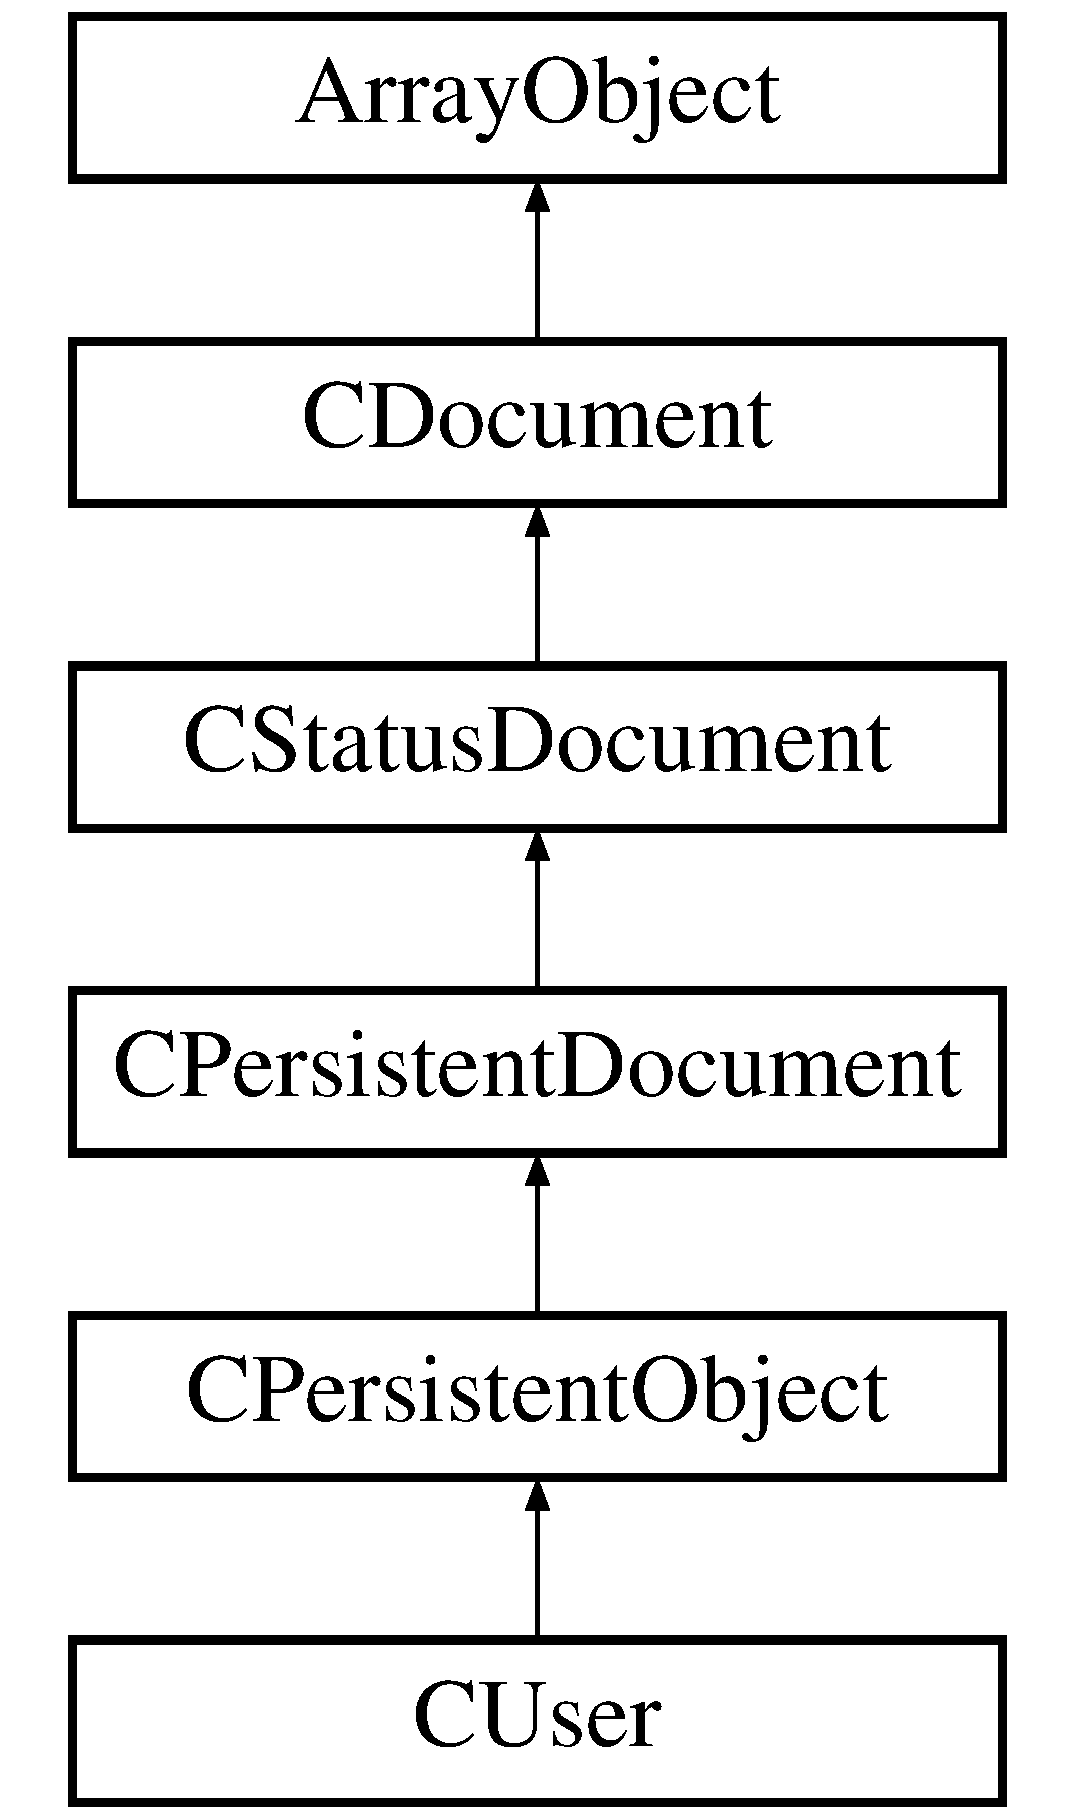
\includegraphics[height=6.000000cm]{class_c_user}
\end{center}
\end{figure}
\subsection*{Public Member Functions}
\begin{DoxyCompactItemize}
\item 
\hyperlink{class_c_user_ab645d29752c93c7c45f711e630691e51}{Name} (\$the\-Value=N\-U\-L\-L, \$get\-Old=F\-A\-L\-S\-E)
\item 
\hyperlink{class_c_user_a67e1a8d936265fbb8a10ccac4b76647a}{Code} (\$the\-Value=N\-U\-L\-L, \$get\-Old=F\-A\-L\-S\-E)
\item 
\hyperlink{class_c_user_a827f71914faf740df88212b8fa2f02a7}{Pass} (\$the\-Value=N\-U\-L\-L, \$get\-Old=F\-A\-L\-S\-E)
\item 
\hyperlink{class_c_user_ac17ab6a51035f9e8074c2602e47ae818}{Mail} (\$the\-Value=N\-U\-L\-L, \$get\-Old=F\-A\-L\-S\-E)
\item 
\hyperlink{class_c_user_add1faba1d336cf4b610a632d3c376dd2}{Role} (\$the\-Value=N\-U\-L\-L, \$the\-Operation=N\-U\-L\-L, \$get\-Old=F\-A\-L\-S\-E)
\item 
\hyperlink{class_c_user_ab0461ec04fd8043c24ec0ef94fadb995}{Profile} (\$the\-Value=N\-U\-L\-L, \$the\-Operation=N\-U\-L\-L, \$get\-Old=F\-A\-L\-S\-E)
\item 
\hyperlink{class_c_user_a09c0c6f7252ac4a3b96457b00ccc6901}{Domain} (\$the\-Value=N\-U\-L\-L, \$the\-Operation=N\-U\-L\-L, \$get\-Old=F\-A\-L\-S\-E)
\item 
\hyperlink{class_c_user_acd45e0c231f54e7ccc452cb6bcd3aa35}{Manager} (\$the\-Value=N\-U\-L\-L, \$get\-Old=F\-A\-L\-S\-E)
\item 
\hyperlink{class_c_user_a8059ecd785bdbb0ab52da79a46dcde6c}{Load\-Manager} (\hyperlink{class_c_connection}{C\-Connection} \$the\-Connection, \$do\-Reload=F\-A\-L\-S\-E)
\end{DoxyCompactItemize}
\subsection*{Static Public Member Functions}
\begin{DoxyCompactItemize}
\item 
static \hyperlink{class_c_user_a9371705ee2fe545cf966b1bf3bd8c574}{Default\-Container\-Name} ()
\item 
static \hyperlink{class_c_user_a41767eb89356bfc787eabbe5596df36d}{Resolve} (\hyperlink{class_c_connection}{C\-Connection} \$the\-Connection, \$the\-Identifier, \$do\-Throw=F\-A\-L\-S\-E)
\end{DoxyCompactItemize}
\subsection*{Protected Member Functions}
\begin{DoxyCompactItemize}
\item 
\hyperlink{class_c_user_afe88b46176ec8227c8ee5d6b1e6e758f}{\-\_\-index} (\hyperlink{class_c_connection}{C\-Connection} \$the\-Connection, \$the\-Modifiers)
\item 
\hyperlink{class_c_user_ac4d911d88bee7897d0fc257f126eb66a}{\-\_\-\-Preset} (\&\$the\-Offset, \&\$the\-Value)
\item 
\hyperlink{class_c_user_a44a9117071cea9d4933c08ef347006d6}{\-\_\-\-Preunset} (\&\$the\-Offset)
\item 
\hyperlink{class_c_user_a9f55517030b5670e0ddadca1004b0b08}{\-\_\-\-Ready} ()
\item 
\hyperlink{class_c_user_af6fe894a0a45226f314057a5c40f3bd1}{\-\_\-\-Precommit\-Related} (\&\$the\-Connection, \&\$the\-Modifiers)
\item 
\hyperlink{class_c_user_aa05407c9768b02801a2a8f47414de1fd}{\-\_\-\-Postcommit\-Cleanup} (\&\$the\-Connection, \&\$the\-Modifiers)
\end{DoxyCompactItemize}
\subsection*{Protected Attributes}
\begin{DoxyCompactItemize}
\item 
\hypertarget{class_c_user_a17d9745db7fcc2f05478bc17c734666f}{{\bfseries \$m\-Manager} = N\-U\-L\-L}\label{class_c_user_a17d9745db7fcc2f05478bc17c734666f}

\end{DoxyCompactItemize}


\subsection{Member Function Documentation}
\hypertarget{class_c_user_afe88b46176ec8227c8ee5d6b1e6e758f}{\index{C\-User@{C\-User}!\-\_\-index@{\-\_\-index}}
\index{\-\_\-index@{\-\_\-index}!CUser@{C\-User}}
\subsubsection[{\-\_\-index}]{\setlength{\rightskip}{0pt plus 5cm}C\-User\-::\-\_\-index (
\begin{DoxyParamCaption}
\item[{{\bf C\-Connection}}]{\$the\-Connection, }
\item[{}]{\$the\-Modifiers}
\end{DoxyParamCaption}
)\hspace{0.3cm}{\ttfamily [protected]}}}\label{class_c_user_afe88b46176ec8227c8ee5d6b1e6e758f}
\subparagraph*{Return the object's global unique identifier}

User identifiers are constituted by the user code, this mathod will simply return it.

In derived classes this can be overloaded.


\begin{DoxyParams}[1]{Parameters}
\hyperlink{class_c_connection}{C\-Connection} & {\em \$the\-Connection} & Server, database or container. \\
\hline
bitfield & {\em \$the\-Modifiers} & Commit options.\\
\hline
\end{DoxyParams}
protected \begin{DoxyReturn}{Returns}
string$|$\-N\-U\-L\-L The object's global unique identifier.
\end{DoxyReturn}
\begin{DoxySeeAlso}{See Also}
k\-T\-A\-G\-\_\-\-L\-I\-D k\-T\-A\-G\-\_\-\-N\-A\-M\-E\-S\-P\-A\-C\-E k\-T\-O\-K\-E\-N\-\_\-\-N\-A\-M\-E\-S\-P\-A\-C\-E\-\_\-\-S\-E\-P\-A\-R\-A\-T\-O\-R 
\end{DoxySeeAlso}
\hypertarget{class_c_user_aa05407c9768b02801a2a8f47414de1fd}{\index{C\-User@{C\-User}!\-\_\-\-Postcommit\-Cleanup@{\-\_\-\-Postcommit\-Cleanup}}
\index{\-\_\-\-Postcommit\-Cleanup@{\-\_\-\-Postcommit\-Cleanup}!CUser@{C\-User}}
\subsubsection[{\-\_\-\-Postcommit\-Cleanup}]{\setlength{\rightskip}{0pt plus 5cm}C\-User\-::\-\_\-\-Postcommit\-Cleanup (
\begin{DoxyParamCaption}
\item[{\&}]{\$the\-Connection, }
\item[{\&}]{\$the\-Modifiers}
\end{DoxyParamCaption}
)\hspace{0.3cm}{\ttfamily [protected]}}}\label{class_c_user_aa05407c9768b02801a2a8f47414de1fd}
\subparagraph*{Cleanup the object after committing}

In this class we reset the manager object cache, we set the data member to {\ttfamily N\-U\-L\-L}, so that next time one wants to retrieve the manager object, it will have to be refreshed and its references actualised.


\begin{DoxyParams}[1]{Parameters}
reference & {\em \&\$the\-Connection} & Server, database or container. \\
\hline
reference & {\em \&\$the\-Modifiers} & Commit options.\\
\hline
\end{DoxyParams}
protected \hypertarget{class_c_user_af6fe894a0a45226f314057a5c40f3bd1}{\index{C\-User@{C\-User}!\-\_\-\-Precommit\-Related@{\-\_\-\-Precommit\-Related}}
\index{\-\_\-\-Precommit\-Related@{\-\_\-\-Precommit\-Related}!CUser@{C\-User}}
\subsubsection[{\-\_\-\-Precommit\-Related}]{\setlength{\rightskip}{0pt plus 5cm}C\-User\-::\-\_\-\-Precommit\-Related (
\begin{DoxyParamCaption}
\item[{\&}]{\$the\-Connection, }
\item[{\&}]{\$the\-Modifiers}
\end{DoxyParamCaption}
)\hspace{0.3cm}{\ttfamily [protected]}}}\label{class_c_user_af6fe894a0a45226f314057a5c40f3bd1}
\subparagraph*{Handle embedded or related objects before committing}

In this class we commit the eventual manager user provided as an object or load the manager if provided as an identifier.


\begin{DoxyParams}[1]{Parameters}
reference & {\em \&\$the\-Connection} & Server, database or container. \\
\hline
reference & {\em \&\$the\-Modifiers} & Commit options.\\
\hline
\end{DoxyParams}
protected \begin{DoxyReturn}{Returns}
mixed 
\end{DoxyReturn}
\hypertarget{class_c_user_ac4d911d88bee7897d0fc257f126eb66a}{\index{C\-User@{C\-User}!\-\_\-\-Preset@{\-\_\-\-Preset}}
\index{\-\_\-\-Preset@{\-\_\-\-Preset}!CUser@{C\-User}}
\subsubsection[{\-\_\-\-Preset}]{\setlength{\rightskip}{0pt plus 5cm}C\-User\-::\-\_\-\-Preset (
\begin{DoxyParamCaption}
\item[{\&}]{\$the\-Offset, }
\item[{\&}]{\$the\-Value}
\end{DoxyParamCaption}
)\hspace{0.3cm}{\ttfamily [protected]}}}\label{class_c_user_ac4d911d88bee7897d0fc257f126eb66a}
\subparagraph*{Handle offset before setting it}

In this class we prevent the modification of the user code if the object has its \hyperlink{class_c_status_document_ab7d96fd4588cf7d5432fc65a1d1fb076}{\-\_\-\-Is\-Committed()} status set. This is because the code represents the user native identifier.

We also ensure that the provided profile is an array.


\begin{DoxyParams}[1]{Parameters}
reference & {\em \&\$the\-Offset} & Offset. \\
\hline
reference & {\em \&\$the\-Value} & Value to set at offset.\\
\hline
\end{DoxyParams}
protected


\begin{DoxyExceptions}{Exceptions}
{\em Exception} & \hyperlink{class_c_status_document_ab7d96fd4588cf7d5432fc65a1d1fb076}{\-\_\-\-Is\-Committed()}\\
\hline
\end{DoxyExceptions}
\begin{DoxySeeAlso}{See Also}
k\-T\-A\-G\-\_\-\-U\-S\-E\-R\-\_\-\-C\-O\-D\-E k\-T\-A\-G\-\_\-\-U\-S\-E\-R\-\_\-\-P\-R\-O\-F\-I\-L\-E 
\end{DoxySeeAlso}
\hypertarget{class_c_user_a44a9117071cea9d4933c08ef347006d6}{\index{C\-User@{C\-User}!\-\_\-\-Preunset@{\-\_\-\-Preunset}}
\index{\-\_\-\-Preunset@{\-\_\-\-Preunset}!CUser@{C\-User}}
\subsubsection[{\-\_\-\-Preunset}]{\setlength{\rightskip}{0pt plus 5cm}C\-User\-::\-\_\-\-Preunset (
\begin{DoxyParamCaption}
\item[{\&}]{\$the\-Offset}
\end{DoxyParamCaption}
)\hspace{0.3cm}{\ttfamily [protected]}}}\label{class_c_user_a44a9117071cea9d4933c08ef347006d6}
\subparagraph*{Handle offset before unsetting it}

In this class we prevent the modification of the user code if the object has its \hyperlink{class_c_status_document_ab7d96fd4588cf7d5432fc65a1d1fb076}{\-\_\-\-Is\-Committed()} status set. This is because the code represents the user native identifier.


\begin{DoxyParams}[1]{Parameters}
reference & {\em \&\$the\-Offset} & Offset.\\
\hline
\end{DoxyParams}
protected


\begin{DoxyExceptions}{Exceptions}
{\em Exception} & \hyperlink{class_c_status_document_ab7d96fd4588cf7d5432fc65a1d1fb076}{\-\_\-\-Is\-Committed()}\\
\hline
\end{DoxyExceptions}
\begin{DoxySeeAlso}{See Also}
k\-T\-A\-G\-\_\-\-U\-S\-E\-R\-\_\-\-C\-O\-D\-E 
\end{DoxySeeAlso}
\hypertarget{class_c_user_a9f55517030b5670e0ddadca1004b0b08}{\index{C\-User@{C\-User}!\-\_\-\-Ready@{\-\_\-\-Ready}}
\index{\-\_\-\-Ready@{\-\_\-\-Ready}!CUser@{C\-User}}
\subsubsection[{\-\_\-\-Ready}]{\setlength{\rightskip}{0pt plus 5cm}C\-User\-::\-\_\-\-Ready (
\begin{DoxyParamCaption}
{}
\end{DoxyParamCaption}
)\hspace{0.3cm}{\ttfamily [protected]}}}\label{class_c_user_a9f55517030b5670e0ddadca1004b0b08}
\subparagraph*{Determine if the object is ready}

In this class we tie the \hyperlink{class_c_status_document_a954dee06e219e0a0f2e7fa6edac56e28}{\-\_\-\-Is\-Inited()} status to the presence or absence of the \hyperlink{}{k\-T\-A\-G\-\_\-\-L\-I\-D} offset.

protected \begin{DoxyReturn}{Returns}
boolean {\ttfamily T\-R\-U\-E} means \hyperlink{}{.  \-\_\-\-Ready()  k\-T\-A\-G\-\_\-\-L\-I\-D }
\end{DoxyReturn}
\hypertarget{class_c_user_a67e1a8d936265fbb8a10ccac4b76647a}{\index{C\-User@{C\-User}!Code@{Code}}
\index{Code@{Code}!CUser@{C\-User}}
\subsubsection[{Code}]{\setlength{\rightskip}{0pt plus 5cm}C\-User\-::\-Code (
\begin{DoxyParamCaption}
\item[{}]{\$the\-Value = {\ttfamily NULL}, }
\item[{}]{\$get\-Old = {\ttfamily FALSE}}
\end{DoxyParamCaption}
)}}\label{class_c_user_a67e1a8d936265fbb8a10ccac4b76647a}
\subparagraph*{Manage user code}

The {\itshape code}, \hyperlink{}{k\-T\-A\-G\-\_\-\-U\-S\-E\-R\-\_\-\-C\-O\-D\-E}, holds the code of the user. This data represents the user native identifier. Once the object has been committed, this attribute will be locked.

The method accepts a parameter which represents either the name or the requested operation, depending on its value\-:


\begin{DoxyItemize}
\item {\ttfamily N\-U\-L\-L}\-: Return the current value. 
\item {\ttfamily F\-A\-L\-S\-E}\-: Delete the current value. 
\item {\itshape other}\-: Set the value with the provided parameter. 
\end{DoxyItemize}

The second parameter is a boolean which if {\ttfamily T\-R\-U\-E} will return the {\itshape old} value when replacing containers; if {\ttfamily F\-A\-L\-S\-E}, it will return the currently set value.


\begin{DoxyParams}[1]{Parameters}
mixed & {\em \$the\-Value} & Value or operation. \\
\hline
boolean & {\em \$get\-Old} & {\ttfamily T\-R\-U\-E} get old value.\\
\hline
\end{DoxyParams}
public \begin{DoxyReturn}{Returns}
mixed {\itshape New} or {\itshape old} value.
\end{DoxyReturn}
Manage\-Offset()

\begin{DoxySeeAlso}{See Also}
k\-T\-A\-G\-\_\-\-U\-S\-E\-R\-\_\-\-C\-O\-D\-E 
\end{DoxySeeAlso}
\hypertarget{class_c_user_a9371705ee2fe545cf966b1bf3bd8c574}{\index{C\-User@{C\-User}!Default\-Container\-Name@{Default\-Container\-Name}}
\index{Default\-Container\-Name@{Default\-Container\-Name}!CUser@{C\-User}}
\subsubsection[{Default\-Container\-Name}]{\setlength{\rightskip}{0pt plus 5cm}static C\-User\-::\-Default\-Container\-Name (
\begin{DoxyParamCaption}
{}
\end{DoxyParamCaption}
)\hspace{0.3cm}{\ttfamily [static]}}}\label{class_c_user_a9371705ee2fe545cf966b1bf3bd8c574}
\subparagraph*{Return the default users container name}

This class uses the \hyperlink{}{k\-C\-O\-N\-T\-A\-I\-N\-E\-R\-\_\-\-U\-S\-E\-R\-\_\-\-N\-A\-M\-E} default name.

\begin{DoxyReturn}{Returns}
string The default container name.
\end{DoxyReturn}

\begin{DoxyExceptions}{Exceptions}
{\em Exception} & \\
\hline
\end{DoxyExceptions}
\begin{DoxySeeAlso}{See Also}
k\-C\-O\-N\-T\-A\-I\-N\-E\-R\-\_\-\-U\-S\-E\-R\-\_\-\-N\-A\-M\-E 
\end{DoxySeeAlso}
\hypertarget{class_c_user_a09c0c6f7252ac4a3b96457b00ccc6901}{\index{C\-User@{C\-User}!Domain@{Domain}}
\index{Domain@{Domain}!CUser@{C\-User}}
\subsubsection[{Domain}]{\setlength{\rightskip}{0pt plus 5cm}C\-User\-::\-Domain (
\begin{DoxyParamCaption}
\item[{}]{\$the\-Value = {\ttfamily NULL}, }
\item[{}]{\$the\-Operation = {\ttfamily NULL}, }
\item[{}]{\$get\-Old = {\ttfamily FALSE}}
\end{DoxyParamCaption}
)}}\label{class_c_user_a09c0c6f7252ac4a3b96457b00ccc6901}
\subparagraph*{Manage user domains}

The user domain, \hyperlink{}{k\-T\-A\-G\-\_\-\-U\-S\-E\-R\-\_\-\-D\-O\-M\-A\-I\-N}, holds a list of unique values that represent the different domains in which the current user is registered.

This offset collects the list of these domains in an enumerated set that can be managed with the following parameters\-:


\begin{DoxyItemize}
\item {\ttfamily \$the\-Value}\-: Depending on the next parameter, this may either refer to the value to be set or to the index of the element to be retrieved or deleted\-: 
\begin{DoxyItemize}
\item {\ttfamily N\-U\-L\-L}\-: This value indicates that we want to operate on all elements, which means, in practical terms, that we either want to retrieve or delete the full list. If the operation parameter resolves to {\ttfamily T\-R\-U\-E}, the method will default to retrieving the current list and no new element will be added. 
\item {\ttfamily array}\-: An array indicates that we want to operate on a list of values and that other parameters may also be provided as lists. Note that \hyperlink{}{Array\-Object} instances are not considered here as arrays. 
\item {\itshape other}\-: Any other type represents either the new value to be added or the index to the value to be returned or deleted. 
\end{DoxyItemize}
\item {\ttfamily \$the\-Operation}\-: This parameter represents the operation to be performed whose scope depends on the value of the previous parameter\-: 
\begin{DoxyItemize}
\item {\ttfamily N\-U\-L\-L}\-: Return the element or full list. 
\item {\ttfamily F\-A\-L\-S\-E}\-: Delete the element or full list. 
\item {\ttfamily array}\-: This type is only considered if the {\ttfamily \$the\-Value} parameter is provided as an array\-: the method will be called for each element of the {\ttfamily \$the\-Value} parameter matched with the corresponding element of this parameter, which also means that both both parameters must share the same count. 
\item {\itshape other}\-: Add the {\ttfamily \$the\-Value} value to the list. If you provided {\ttfamily N\-U\-L\-L} in the previous parameter, the operation will be reset to {\ttfamily N\-U\-L\-L}. 
\end{DoxyItemize}
\item {\ttfamily \$get\-Old}\-: Determines what the method will return\-: 
\begin{DoxyItemize}
\item {\ttfamily T\-R\-U\-E}\-: Return the value {\itshape before} it was eventually modified. 
\item {\ttfamily F\-A\-L\-S\-E}\-: Return the value {\itshape after} it was eventually modified. 
\end{DoxyItemize}
\end{DoxyItemize}


\begin{DoxyParams}[1]{Parameters}
mixed & {\em \$the\-Value} & Value or index. \\
\hline
mixed & {\em \$the\-Operation} & Operation. \\
\hline
boolean & {\em \$get\-Old} & T\-R\-U\-E get old value.\\
\hline
\end{DoxyParams}
public \begin{DoxyReturn}{Returns}
mixed {\itshape New} or {\itshape old} domain.
\end{DoxyReturn}
Manage\-Object\-Set\-Offset()

\begin{DoxySeeAlso}{See Also}
k\-T\-A\-G\-\_\-\-U\-S\-E\-R\-\_\-\-D\-O\-M\-A\-I\-N 
\end{DoxySeeAlso}
\hypertarget{class_c_user_a8059ecd785bdbb0ab52da79a46dcde6c}{\index{C\-User@{C\-User}!Load\-Manager@{Load\-Manager}}
\index{Load\-Manager@{Load\-Manager}!CUser@{C\-User}}
\subsubsection[{Load\-Manager}]{\setlength{\rightskip}{0pt plus 5cm}C\-User\-::\-Load\-Manager (
\begin{DoxyParamCaption}
\item[{{\bf C\-Connection}}]{\$the\-Connection, }
\item[{}]{\$do\-Reload = {\ttfamily FALSE}}
\end{DoxyParamCaption}
)}}\label{class_c_user_a8059ecd785bdbb0ab52da79a46dcde6c}
\subparagraph*{Load manager object}

This method will return the current manager object\-: if the term is not set, the method will return {\ttfamily N\-U\-L\-L}; if the manager cannot be found, the method will raise an exception.

The object will also be loaded in a data member that can function as a cache.

The method features two parameters\-: the first refers to the container in which the manager is stored, the second is a boolean flag that determines whether the object is to be read, or if the cached copy can be used.


\begin{DoxyParams}[1]{Parameters}
\hyperlink{class_c_connection}{C\-Connection} & {\em \$the\-Connection} & Server, database or container. \\
\hline
boolean & {\em \$do\-Reload} & Reload if {\ttfamily T\-R\-U\-E}.\\
\hline
\end{DoxyParams}
public \begin{DoxyReturn}{Returns}
\hyperlink{class_c_ontology_term}{C\-Ontology\-Term} Manager object or {\ttfamily N\-U\-L\-L}.
\end{DoxyReturn}

\begin{DoxyExceptions}{Exceptions}
{\em Exception} & \hyperlink{class_c_persistent_object_a5a5402ef394104148cfc580a6799ac2b}{New\-Object()}\\
\hline
\end{DoxyExceptions}
\begin{DoxySeeAlso}{See Also}
k\-T\-A\-G\-\_\-\-U\-S\-E\-R\-\_\-\-M\-A\-N\-A\-G\-E\-R 
\end{DoxySeeAlso}
\hypertarget{class_c_user_ac17ab6a51035f9e8074c2602e47ae818}{\index{C\-User@{C\-User}!Mail@{Mail}}
\index{Mail@{Mail}!CUser@{C\-User}}
\subsubsection[{Mail}]{\setlength{\rightskip}{0pt plus 5cm}C\-User\-::\-Mail (
\begin{DoxyParamCaption}
\item[{}]{\$the\-Value = {\ttfamily NULL}, }
\item[{}]{\$get\-Old = {\ttfamily FALSE}}
\end{DoxyParamCaption}
)}}\label{class_c_user_ac17ab6a51035f9e8074c2602e47ae818}
\subparagraph*{Manage user mail}

The {\itshape mail}, \hyperlink{}{k\-T\-A\-G\-\_\-\-U\-S\-E\-R\-\_\-\-M\-A\-I\-L}, holds the user e-\/mail address.

The method accepts a parameter which represents either the name or the requested operation, depending on its value\-:


\begin{DoxyItemize}
\item {\ttfamily N\-U\-L\-L}\-: Return the current value. 
\item {\ttfamily F\-A\-L\-S\-E}\-: Delete the current value. 
\item {\itshape other}\-: Set the value with the provided parameter. 
\end{DoxyItemize}

The second parameter is a boolean which if {\ttfamily T\-R\-U\-E} will return the {\itshape old} value when replacing containers; if {\ttfamily F\-A\-L\-S\-E}, it will return the currently set value.


\begin{DoxyParams}[1]{Parameters}
mixed & {\em \$the\-Value} & Value or operation. \\
\hline
boolean & {\em \$get\-Old} & {\ttfamily T\-R\-U\-E} get old value.\\
\hline
\end{DoxyParams}
public \begin{DoxyReturn}{Returns}
mixed {\itshape New} or {\itshape old} value.
\end{DoxyReturn}
Manage\-Offset()

\begin{DoxySeeAlso}{See Also}
k\-T\-A\-G\-\_\-\-U\-S\-E\-R\-\_\-\-M\-A\-I\-L 
\end{DoxySeeAlso}
\hypertarget{class_c_user_acd45e0c231f54e7ccc452cb6bcd3aa35}{\index{C\-User@{C\-User}!Manager@{Manager}}
\index{Manager@{Manager}!CUser@{C\-User}}
\subsubsection[{Manager}]{\setlength{\rightskip}{0pt plus 5cm}C\-User\-::\-Manager (
\begin{DoxyParamCaption}
\item[{}]{\$the\-Value = {\ttfamily NULL}, }
\item[{}]{\$get\-Old = {\ttfamily FALSE}}
\end{DoxyParamCaption}
)}}\label{class_c_user_acd45e0c231f54e7ccc452cb6bcd3aa35}
\subparagraph*{Manage user manager}

The {\itshape mamager}, \hyperlink{}{k\-T\-A\-G\-\_\-\-U\-S\-E\-R\-\_\-\-M\-A\-N\-A\-G\-E\-R}, holds the reference to another user who has the responsibility and task of managing the current user. In general this will refer to the user that created the current user and that can revoke privileges or delete the user.

The method accepts a parameter which represents either the code of the user's manager or the requested operation, depending on its value\-:


\begin{DoxyItemize}
\item {\ttfamily N\-U\-L\-L}\-: Return the current value. 
\item {\ttfamily F\-A\-L\-S\-E}\-: Delete the current value. 
\item {\itshape other}\-: Set the value with the provided parameter. 
\end{DoxyItemize}

The second parameter is a boolean which if {\ttfamily T\-R\-U\-E} will return the {\itshape old} value when replacing containers; if {\ttfamily F\-A\-L\-S\-E}, it will return the currently set value.


\begin{DoxyParams}[1]{Parameters}
mixed & {\em \$the\-Value} & Value or operation. \\
\hline
boolean & {\em \$get\-Old} & {\ttfamily T\-R\-U\-E} get old value.\\
\hline
\end{DoxyParams}
public \begin{DoxyReturn}{Returns}
mixed {\itshape New} or {\itshape old} value.
\end{DoxyReturn}
Manage\-Offset()

\begin{DoxySeeAlso}{See Also}
k\-T\-A\-G\-\_\-\-U\-S\-E\-R\-\_\-\-M\-A\-N\-A\-G\-E\-R 
\end{DoxySeeAlso}
\hypertarget{class_c_user_ab645d29752c93c7c45f711e630691e51}{\index{C\-User@{C\-User}!Name@{Name}}
\index{Name@{Name}!CUser@{C\-User}}
\subsubsection[{Name}]{\setlength{\rightskip}{0pt plus 5cm}C\-User\-::\-Name (
\begin{DoxyParamCaption}
\item[{}]{\$the\-Value = {\ttfamily NULL}, }
\item[{}]{\$get\-Old = {\ttfamily FALSE}}
\end{DoxyParamCaption}
)}}\label{class_c_user_ab645d29752c93c7c45f711e630691e51}
\subparagraph*{Manage user name}

The {\itshape name}, \hyperlink{}{k\-T\-A\-G\-\_\-\-U\-S\-E\-R\-\_\-\-N\-A\-M\-E}, holds the full name of the user.

The method accepts a parameter which represents either the name or the requested operation, depending on its value\-:


\begin{DoxyItemize}
\item {\ttfamily N\-U\-L\-L}\-: Return the current value. 
\item {\ttfamily F\-A\-L\-S\-E}\-: Delete the current value. 
\item {\itshape other}\-: Set the value with the provided parameter. 
\end{DoxyItemize}

The second parameter is a boolean which if {\ttfamily T\-R\-U\-E} will return the {\itshape old} value when replacing containers; if {\ttfamily F\-A\-L\-S\-E}, it will return the currently set value.


\begin{DoxyParams}[1]{Parameters}
mixed & {\em \$the\-Value} & Value or operation. \\
\hline
boolean & {\em \$get\-Old} & {\ttfamily T\-R\-U\-E} get old value.\\
\hline
\end{DoxyParams}
public \begin{DoxyReturn}{Returns}
mixed {\itshape New} or {\itshape old} value.
\end{DoxyReturn}
Manage\-Offset()

\begin{DoxySeeAlso}{See Also}
k\-T\-A\-G\-\_\-\-U\-S\-E\-R\-\_\-\-N\-A\-M\-E 
\end{DoxySeeAlso}
\hypertarget{class_c_user_a827f71914faf740df88212b8fa2f02a7}{\index{C\-User@{C\-User}!Pass@{Pass}}
\index{Pass@{Pass}!CUser@{C\-User}}
\subsubsection[{Pass}]{\setlength{\rightskip}{0pt plus 5cm}C\-User\-::\-Pass (
\begin{DoxyParamCaption}
\item[{}]{\$the\-Value = {\ttfamily NULL}, }
\item[{}]{\$get\-Old = {\ttfamily FALSE}}
\end{DoxyParamCaption}
)}}\label{class_c_user_a827f71914faf740df88212b8fa2f02a7}
\subparagraph*{Manage user password}

The {\itshape password}, \hyperlink{}{k\-T\-A\-G\-\_\-\-U\-S\-E\-R\-\_\-\-P\-A\-S\-S}, holds the password of the user. This data along with the user code is used as the login credentials.

The method accepts a parameter which represents either the name or the requested operation, depending on its value\-:


\begin{DoxyItemize}
\item {\ttfamily N\-U\-L\-L}\-: Return the current value. 
\item {\ttfamily F\-A\-L\-S\-E}\-: Delete the current value. 
\item {\itshape other}\-: Set the value with the provided parameter. 
\end{DoxyItemize}

The second parameter is a boolean which if {\ttfamily T\-R\-U\-E} will return the {\itshape old} value when replacing containers; if {\ttfamily F\-A\-L\-S\-E}, it will return the currently set value.


\begin{DoxyParams}[1]{Parameters}
mixed & {\em \$the\-Value} & Value or operation. \\
\hline
boolean & {\em \$get\-Old} & {\ttfamily T\-R\-U\-E} get old value.\\
\hline
\end{DoxyParams}
public \begin{DoxyReturn}{Returns}
mixed {\itshape New} or {\itshape old} value.
\end{DoxyReturn}
Manage\-Offset()

\begin{DoxySeeAlso}{See Also}
k\-T\-A\-G\-\_\-\-U\-S\-E\-R\-\_\-\-P\-A\-S\-S 
\end{DoxySeeAlso}
\hypertarget{class_c_user_ab0461ec04fd8043c24ec0ef94fadb995}{\index{C\-User@{C\-User}!Profile@{Profile}}
\index{Profile@{Profile}!CUser@{C\-User}}
\subsubsection[{Profile}]{\setlength{\rightskip}{0pt plus 5cm}C\-User\-::\-Profile (
\begin{DoxyParamCaption}
\item[{}]{\$the\-Value = {\ttfamily NULL}, }
\item[{}]{\$the\-Operation = {\ttfamily NULL}, }
\item[{}]{\$get\-Old = {\ttfamily FALSE}}
\end{DoxyParamCaption}
)}}\label{class_c_user_ab0461ec04fd8043c24ec0ef94fadb995}
\subparagraph*{Manage user profile set}

The profile set, \hyperlink{}{k\-T\-A\-G\-\_\-\-U\-S\-E\-R\-\_\-\-P\-R\-O\-F\-I\-L\-E}, holds a list of unique values that represent the different privileges and capabilities of the user. This information is not specific to the hosting system, but rather to the library that manages users.

This offset collects the list of these qualifications in an enumerated set that can be managed with the following parameters\-:


\begin{DoxyItemize}
\item {\ttfamily \$the\-Value}\-: Depending on the next parameter, this may either refer to the value to be set or to the index of the element to be retrieved or deleted\-: 
\begin{DoxyItemize}
\item {\ttfamily N\-U\-L\-L}\-: This value indicates that we want to operate on all elements, which means, in practical terms, that we either want to retrieve or delete the full list. If the operation parameter resolves to {\ttfamily T\-R\-U\-E}, the method will default to retrieving the current list and no new element will be added. 
\item {\ttfamily array}\-: An array indicates that we want to operate on a list of values and that other parameters may also be provided as lists. Note that \hyperlink{}{Array\-Object} instances are not considered here as arrays. 
\item {\itshape other}\-: Any other type represents either the new value to be added or the index to the value to be returned or deleted. 
\end{DoxyItemize}
\item {\ttfamily \$the\-Operation}\-: This parameter represents the operation to be performed whose scope depends on the value of the previous parameter\-: 
\begin{DoxyItemize}
\item {\ttfamily N\-U\-L\-L}\-: Return the element or full list. 
\item {\ttfamily F\-A\-L\-S\-E}\-: Delete the element or full list. 
\item {\ttfamily array}\-: This type is only considered if the {\ttfamily \$the\-Value} parameter is provided as an array\-: the method will be called for each element of the {\ttfamily \$the\-Value} parameter matched with the corresponding element of this parameter, which also means that both both parameters must share the same count. 
\item {\itshape other}\-: Add the {\ttfamily \$the\-Value} value to the list. If you provided {\ttfamily N\-U\-L\-L} in the previous parameter, the operation will be reset to {\ttfamily N\-U\-L\-L}. 
\end{DoxyItemize}
\item {\ttfamily \$get\-Old}\-: Determines what the method will return\-: 
\begin{DoxyItemize}
\item {\ttfamily T\-R\-U\-E}\-: Return the value {\itshape before} it was eventually modified. 
\item {\ttfamily F\-A\-L\-S\-E}\-: Return the value {\itshape after} it was eventually modified. 
\end{DoxyItemize}
\end{DoxyItemize}


\begin{DoxyParams}[1]{Parameters}
mixed & {\em \$the\-Value} & Value or index. \\
\hline
mixed & {\em \$the\-Operation} & Operation. \\
\hline
boolean & {\em \$get\-Old} & T\-R\-U\-E get old value.\\
\hline
\end{DoxyParams}
public \begin{DoxyReturn}{Returns}
mixed {\itshape New} or {\itshape old} kind.
\end{DoxyReturn}
Manage\-Object\-Set\-Offset()

\begin{DoxySeeAlso}{See Also}
k\-T\-A\-G\-\_\-\-U\-S\-E\-R\-\_\-\-P\-R\-O\-F\-I\-L\-E 
\end{DoxySeeAlso}
\hypertarget{class_c_user_a41767eb89356bfc787eabbe5596df36d}{\index{C\-User@{C\-User}!Resolve@{Resolve}}
\index{Resolve@{Resolve}!CUser@{C\-User}}
\subsubsection[{Resolve}]{\setlength{\rightskip}{0pt plus 5cm}static C\-User\-::\-Resolve (
\begin{DoxyParamCaption}
\item[{{\bf C\-Connection}}]{\$the\-Connection, }
\item[{}]{\$the\-Identifier, }
\item[{}]{\$do\-Throw = {\ttfamily FALSE}}
\end{DoxyParamCaption}
)\hspace{0.3cm}{\ttfamily [static]}}}\label{class_c_user_a41767eb89356bfc787eabbe5596df36d}
\subparagraph*{Resolve a user}

This method can be used to locate a user given the attributes that comprise its identifier.

The method accepts the following parameters\-:


\begin{DoxyItemize}
\item {\ttfamily \$the\-Connection}\-: This parameter represents the connection from which the terms container must be resolved. If this parameter cannot be correctly determined, the method will raise an exception. 
\item {\ttfamily \$the\-Identifier}\-: In this class by default the native identifier is the user code, we assume this parameter is that string. 
\item {\ttfamily \$do\-Throw}\-: If {\ttfamily T\-R\-U\-E}, any failure to resolve the term or its namespace, will raise an exception. 
\end{DoxyItemize}

The method will return the found user, {\ttfamily N\-U\-L\-L} if not found, or raise an exception if the last parameter is {\ttfamily T\-R\-U\-E}.

{\bfseries Note\-: do not provide an array containing the object in the identifier parameter, or you will get unexpected results.}


\begin{DoxyParams}[1]{Parameters}
\hyperlink{class_c_connection}{C\-Connection} & {\em \$the\-Connection} & Server, database or container. \\
\hline
mixed & {\em \$the\-Identifier} & User identifier or user reference. \\
\hline
boolean & {\em \$do\-Throw} & If {\ttfamily T\-R\-U\-E} raise an exception.\\
\hline
\end{DoxyParams}
\begin{DoxyReturn}{Returns}
\hyperlink{class_c_user}{C\-User} Matched user or {\ttfamily N\-U\-L\-L}.
\end{DoxyReturn}

\begin{DoxyExceptions}{Exceptions}
{\em Exception} & \\
\hline
\end{DoxyExceptions}
\hypertarget{class_c_user_add1faba1d336cf4b610a632d3c376dd2}{\index{C\-User@{C\-User}!Role@{Role}}
\index{Role@{Role}!CUser@{C\-User}}
\subsubsection[{Role}]{\setlength{\rightskip}{0pt plus 5cm}C\-User\-::\-Role (
\begin{DoxyParamCaption}
\item[{}]{\$the\-Value = {\ttfamily NULL}, }
\item[{}]{\$the\-Operation = {\ttfamily NULL}, }
\item[{}]{\$get\-Old = {\ttfamily FALSE}}
\end{DoxyParamCaption}
)}}\label{class_c_user_add1faba1d336cf4b610a632d3c376dd2}
\subparagraph*{Manage user roles}

The {\itshape role}, \hyperlink{}{k\-T\-A\-G\-\_\-\-U\-S\-E\-R\-\_\-\-R\-O\-L\-E}, holds the list of roles of the user according to the hosting system. It is a string that identifies the user role specific to the hosting operating system or framework.


\begin{DoxyItemize}
\item {\ttfamily \$the\-Value}\-: Depending on the next parameter, this may either refer to the value to be set or to the index of the element to be retrieved or deleted\-: 
\begin{DoxyItemize}
\item {\ttfamily N\-U\-L\-L}\-: This value indicates that we want to operate on all elements, which means, in practical terms, that we either want to retrieve or delete the full list. If the operation parameter resolves to {\ttfamily T\-R\-U\-E}, the method will default to retrieving the current list and no new element will be added. 
\item {\ttfamily array}\-: An array indicates that we want to operate on a list of values and that other parameters may also be provided as lists. Note that \hyperlink{}{Array\-Object} instances are not considered here as arrays. 
\item {\itshape other}\-: Any other type represents either the new value to be added or the index to the value to be returned or deleted. 
\end{DoxyItemize}
\item {\ttfamily \$the\-Operation}\-: This parameter represents the operation to be performed whose scope depends on the value of the previous parameter\-: 
\begin{DoxyItemize}
\item {\ttfamily N\-U\-L\-L}\-: Return the element or full list. 
\item {\ttfamily F\-A\-L\-S\-E}\-: Delete the element or full list. 
\item {\ttfamily array}\-: This type is only considered if the {\ttfamily \$the\-Value} parameter is provided as an array\-: the method will be called for each element of the {\ttfamily \$the\-Value} parameter matched with the corresponding element of this parameter, which also means that both both parameters must share the same count. 
\item {\itshape other}\-: Add the {\ttfamily \$the\-Value} value to the list. If you provided {\ttfamily N\-U\-L\-L} in the previous parameter, the operation will be reset to {\ttfamily N\-U\-L\-L}. 
\end{DoxyItemize}
\item {\ttfamily \$get\-Old}\-: Determines what the method will return\-: 
\begin{DoxyItemize}
\item {\ttfamily T\-R\-U\-E}\-: Return the value {\itshape before} it was eventually modified. 
\item {\ttfamily F\-A\-L\-S\-E}\-: Return the value {\itshape after} it was eventually modified. 
\end{DoxyItemize}
\end{DoxyItemize}


\begin{DoxyParams}[1]{Parameters}
mixed & {\em \$the\-Value} & Value or index. \\
\hline
mixed & {\em \$the\-Operation} & Operation. \\
\hline
boolean & {\em \$get\-Old} & T\-R\-U\-E get old value.\\
\hline
\end{DoxyParams}
public \begin{DoxyReturn}{Returns}
mixed {\itshape New} or {\itshape old} value.
\end{DoxyReturn}
Manage\-Object\-Set\-Offset()

\begin{DoxySeeAlso}{See Also}
k\-T\-A\-G\-\_\-\-U\-S\-E\-R\-\_\-\-R\-O\-L\-E 
\end{DoxySeeAlso}


The documentation for this class was generated from the following file\-:\begin{DoxyCompactItemize}
\item 
/\-Library/\-Web\-Server/\-Library/\-P\-H\-P\-Wrapper/classes/C\-User.\-php\end{DoxyCompactItemize}

\hypertarget{class_c_wrapper}{\section{C\-Wrapper Class Reference}
\label{class_c_wrapper}\index{C\-Wrapper@{C\-Wrapper}}
}
Inheritance diagram for C\-Wrapper\-:\begin{figure}[H]
\begin{center}
\leavevmode
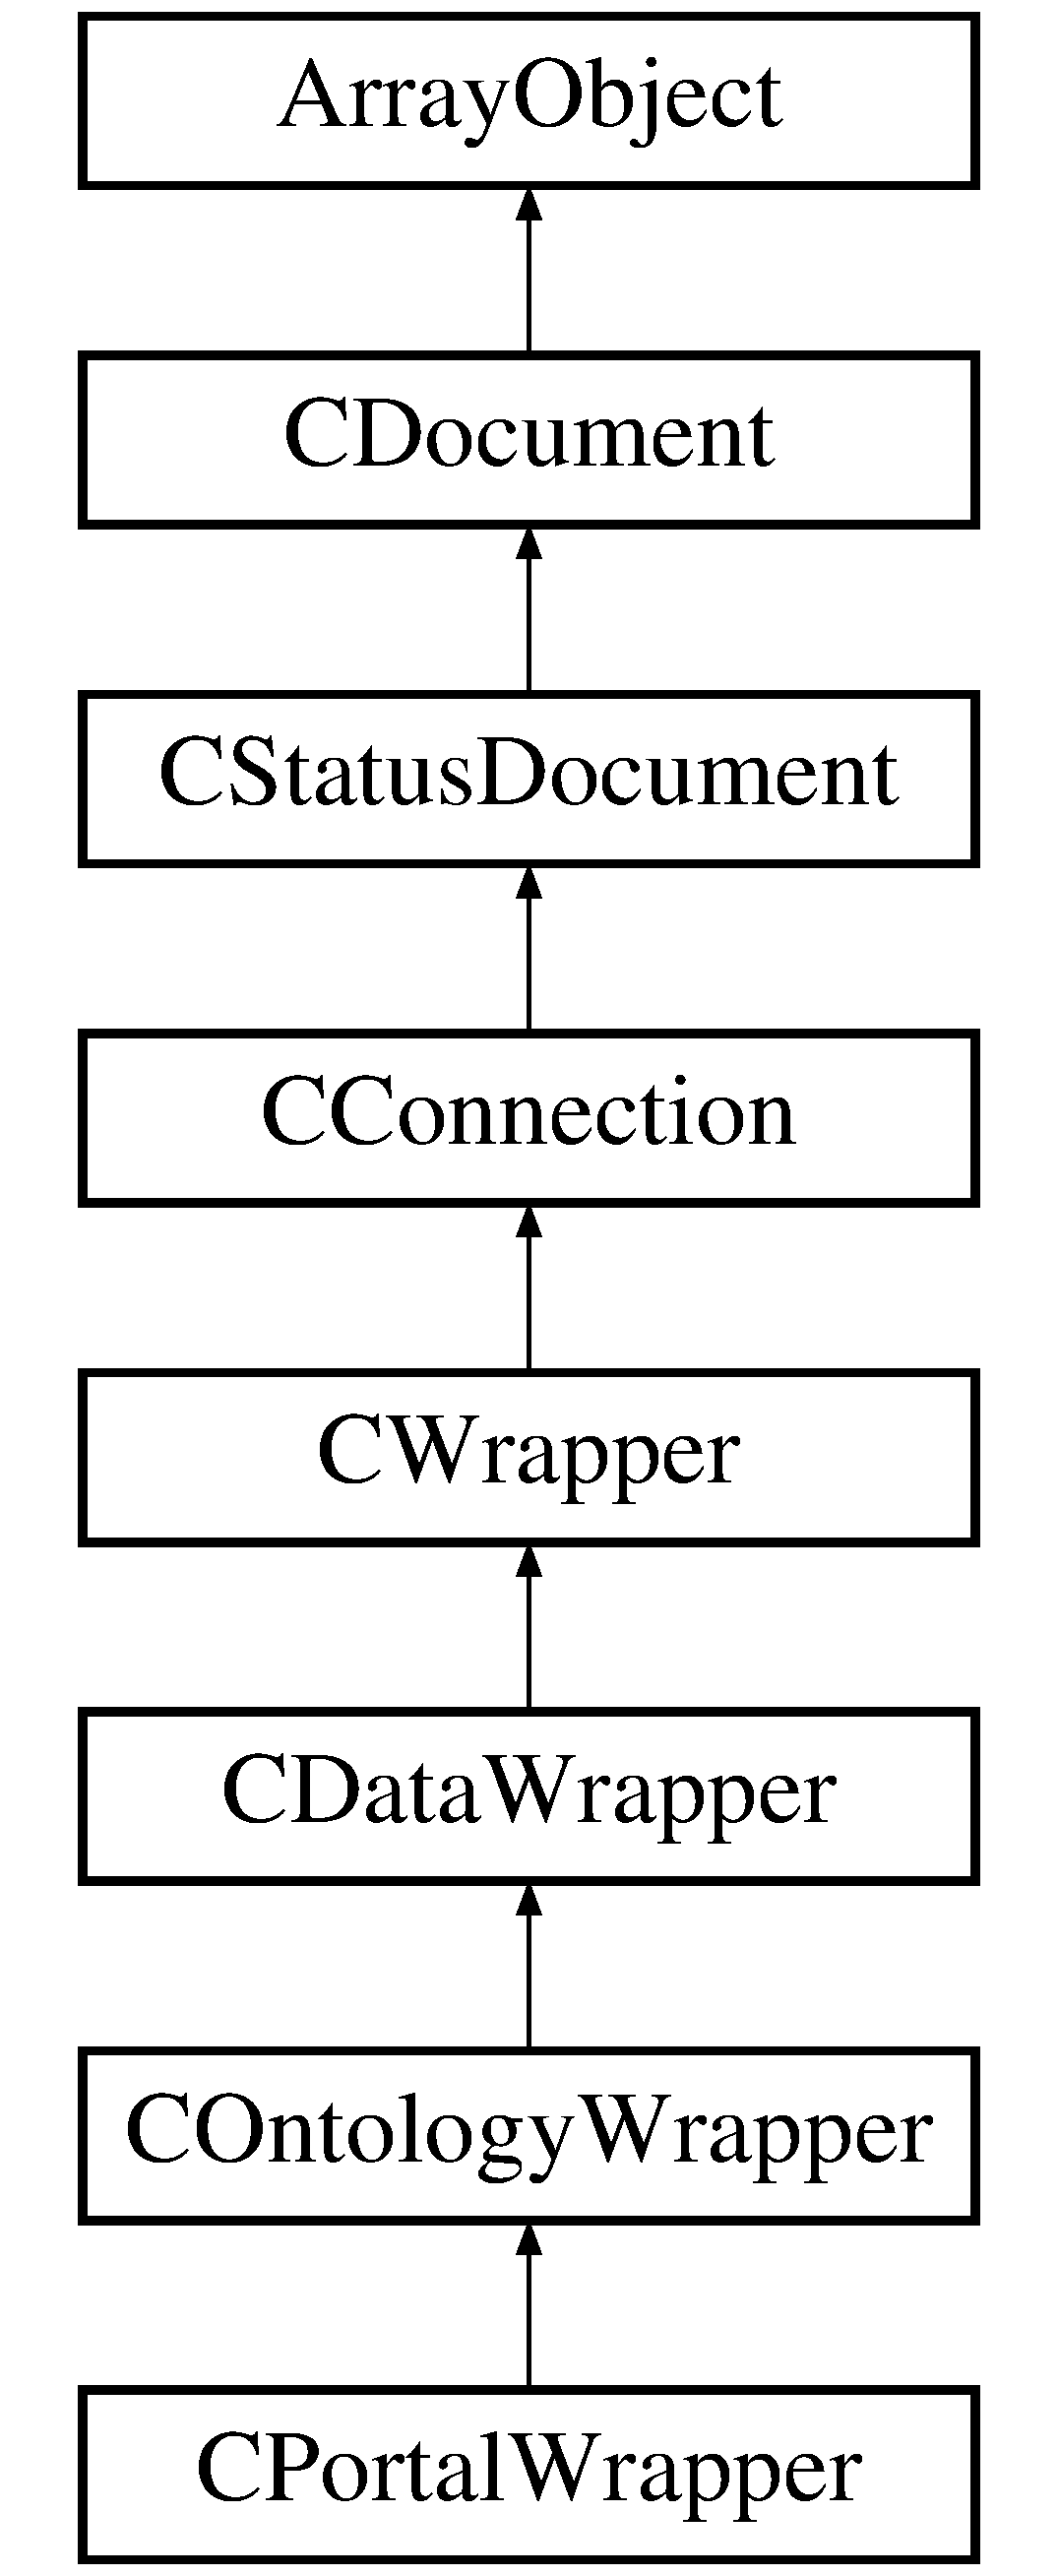
\includegraphics[height=8.000000cm]{class_c_wrapper}
\end{center}
\end{figure}
\subsection*{Public Member Functions}
\begin{DoxyCompactItemize}
\item 
\hyperlink{class_c_wrapper_ab5f77aac3044e183886395ad553fa13a}{\-\_\-\-\_\-construct} (\$the\-Connection=N\-U\-L\-L, \$the\-Options=N\-U\-L\-L)
\item 
\hyperlink{class_c_wrapper_ac9ca75e8d8d1f965218bece1ef55c003}{\-\_\-\-\_\-to\-String} ()
\item 
\hyperlink{class_c_wrapper_a0e605ca2cdd718ecdeb6f3be9b1f0162}{Handle\-Request} ()
\end{DoxyCompactItemize}
\subsection*{Static Public Attributes}
\begin{DoxyCompactItemize}
\item 
\hypertarget{class_c_wrapper_af2a7faae3b12ef8feb3dc840bf61e149}{static {\bfseries \$s\-Parameter\-List} = array( k\-A\-P\-I\-\_\-\-S\-T\-A\-M\-P\-\_\-\-R\-E\-Q\-U\-E\-S\-T, k\-A\-P\-I\-\_\-\-L\-O\-G\-\_\-\-R\-E\-Q\-U\-E\-S\-T, k\-A\-P\-I\-\_\-\-L\-O\-G\-\_\-\-T\-R\-A\-C\-E )}\label{class_c_wrapper_af2a7faae3b12ef8feb3dc840bf61e149}

\end{DoxyCompactItemize}
\subsection*{Protected Member Functions}
\begin{DoxyCompactItemize}
\item 
\hyperlink{class_c_wrapper_a8369eec2e53b3f6394a35bcd919d8779}{\-\_\-\-Init\-Status} ()
\item 
\hyperlink{class_c_wrapper_a2ce212bc7543b4ed07dbc93282d298f6}{\-\_\-\-Init\-Parameters} ()
\item 
\hyperlink{class_c_wrapper_aec2fa3594e36a380d66743b47c24490c}{\-\_\-\-Init\-Options} ()
\item 
\hyperlink{class_c_wrapper_a0e5c5488fce4b388e43dcf6810874d74}{\-\_\-\-Init\-Resources} ()
\item 
\hyperlink{class_c_wrapper_a6675c744053f1b05547ad28fc50a79e6}{\-\_\-\-Parse\-Request} ()
\item 
\hyperlink{class_c_wrapper_a2a3d95961650654468789883ab1607e5}{\-\_\-\-Format\-Request} ()
\item 
\hyperlink{class_c_wrapper_a24b22cfd0022c1cba1741fb294fba5ba}{\-\_\-\-Validate\-Request} ()
\item 
\hyperlink{class_c_wrapper_a53d59f3a61137b8d6f5707d794e2961a}{\-\_\-\-Parse\-Format} ()
\item 
\hyperlink{class_c_wrapper_aa090c135ca1085f46d8cddd393131ea6}{\-\_\-\-Parse\-Operation} ()
\item 
\hyperlink{class_c_wrapper_a13421345af75888b1fa8bcd3381b52a5}{\-\_\-\-Parse\-Timing} ()
\item 
\hyperlink{class_c_wrapper_a8994ff7a5f94438da1c5e3505b145dbd}{\-\_\-\-Validate\-Format} ()
\item 
\hyperlink{class_c_wrapper_aab3f7b2ca4cd9e692c35510d753918a4}{\-\_\-\-Validate\-Operation} ()
\item 
\hyperlink{class_c_wrapper_a12c1dd1f1d1cf0ae889cc19ff17ced0e}{\-\_\-\-Handle\-Request} ()
\item 
\hyperlink{class_c_wrapper_aeff4d2ab12617c1dda2bed705a6969bb}{\-\_\-\-Handle\-\_\-\-List\-Op} (\&\$the\-List)
\item 
\hyperlink{class_c_wrapper_ab58ee7076059e0f992c2a642043b764f}{\-\_\-\-Handle\-\_\-\-Ping} ()
\item 
\hyperlink{class_c_wrapper_aff9eb1799c8f30cb33967c7a50ce6395}{\-\_\-\-Offset\-Manage} (\$the\-Block, \$the\-Element, \$the\-Value=N\-U\-L\-L)
\item 
\hyperlink{class_c_wrapper_ad8dd05c155df0d8fe19be35d4bb67b56}{\-\_\-\-Exception2\-Status} (Exception \$the\-Exception)
\item 
\hyperlink{class_c_wrapper_a60583bacf329d484d01df9851602759f}{\-\_\-\-Encode\-Response} ()
\item 
\hyperlink{class_c_wrapper_a9b96298777cc3aa5817a2039fc8f29bc}{\-\_\-\-Decode\-Parameter} (\$the\-Parameter)
\end{DoxyCompactItemize}
\subsection*{Additional Inherited Members}


\subsection{Constructor \& Destructor Documentation}
\hypertarget{class_c_wrapper_ab5f77aac3044e183886395ad553fa13a}{\index{C\-Wrapper@{C\-Wrapper}!\-\_\-\-\_\-construct@{\-\_\-\-\_\-construct}}
\index{\-\_\-\-\_\-construct@{\-\_\-\-\_\-construct}!CWrapper@{C\-Wrapper}}
\subsubsection[{\-\_\-\-\_\-construct}]{\setlength{\rightskip}{0pt plus 5cm}C\-Wrapper\-::\-\_\-\-\_\-construct (
\begin{DoxyParamCaption}
\item[{}]{\$the\-Connection = {\ttfamily NULL}, }
\item[{}]{\$the\-Options = {\ttfamily NULL}}
\end{DoxyParamCaption}
)}}\label{class_c_wrapper_ab5f77aac3044e183886395ad553fa13a}
Instantiate class.

The constructor will set-\/up the environment and parse the request. The workflow is as follows\-:


\begin{DoxyItemize}
\item {\itshape Check required elements}\-: The method will check if all required elements of the request are there, only if this is the case will the constructor init the service. 
\item {\itshape \hyperlink{class_c_wrapper_a8369eec2e53b3f6394a35bcd919d8779}{\-\_\-\-Init\-Status()}}\-: The response status will be initialised to the \hyperlink{}{k\-S\-T\-A\-T\-U\-S\-\_\-\-I\-D\-L\-E} state. 
\item {\itshape \hyperlink{class_c_wrapper_aec2fa3594e36a380d66743b47c24490c}{\-\_\-\-Init\-Options()}}\-: Service options will be initialised. 
\item {\itshape \hyperlink{class_c_wrapper_a0e5c5488fce4b388e43dcf6810874d74}{\-\_\-\-Init\-Resources()}}\-: Eventual resources are initialised. 
\item {\itshape \hyperlink{class_c_wrapper_a6675c744053f1b05547ad28fc50a79e6}{\-\_\-\-Parse\-Request()}}\-: The request is parsed. 
\item {\itshape \hyperlink{class_c_wrapper_a2a3d95961650654468789883ab1607e5}{\-\_\-\-Format\-Request()}}\-: The request is normalised if necessary. 
\item {\itshape \hyperlink{class_c_wrapper_a24b22cfd0022c1cba1741fb294fba5ba}{\-\_\-\-Validate\-Request()}}\-: The request is validated. 
\end{DoxyItemize}

This protected interface should be overloaded by derived classes to implement custom services.


\begin{DoxyParams}[1]{Parameters}
mixed & {\em \$the\-Connection} & Native connection. \\
\hline
mixed & {\em \$the\-Options} & Connection options.\\
\hline
\end{DoxyParams}
public

\hyperlink{class_c_wrapper_a8369eec2e53b3f6394a35bcd919d8779}{\-\_\-\-Init\-Status()}  \hyperlink{class_c_wrapper_aec2fa3594e36a380d66743b47c24490c}{\-\_\-\-Init\-Options()}  \hyperlink{class_c_wrapper_a0e5c5488fce4b388e43dcf6810874d74}{\-\_\-\-Init\-Resources()}  \hyperlink{class_c_wrapper_a6675c744053f1b05547ad28fc50a79e6}{\-\_\-\-Parse\-Request()}  \hyperlink{class_c_wrapper_a2a3d95961650654468789883ab1607e5}{\-\_\-\-Format\-Request()}  \hyperlink{class_c_wrapper_a24b22cfd0022c1cba1741fb294fba5ba}{\-\_\-\-Validate\-Request()}  \hyperlink{class_c_wrapper_ad8dd05c155df0d8fe19be35d4bb67b56}{\-\_\-\-Exception2\-Status()}  \hyperlink{class_c_wrapper_a60583bacf329d484d01df9851602759f}{\-\_\-\-Encode\-Response()} 

\subsection{Member Function Documentation}
\hypertarget{class_c_wrapper_ac9ca75e8d8d1f965218bece1ef55c003}{\index{C\-Wrapper@{C\-Wrapper}!\-\_\-\-\_\-to\-String@{\-\_\-\-\_\-to\-String}}
\index{\-\_\-\-\_\-to\-String@{\-\_\-\-\_\-to\-String}!CWrapper@{C\-Wrapper}}
\subsubsection[{\-\_\-\-\_\-to\-String}]{\setlength{\rightskip}{0pt plus 5cm}C\-Wrapper\-::\-\_\-\-\_\-to\-String (
\begin{DoxyParamCaption}
{}
\end{DoxyParamCaption}
)}}\label{class_c_wrapper_ac9ca75e8d8d1f965218bece1ef55c003}
\subparagraph*{Return wrapper name}

This method should return the current wrapper's name.

In this class we return the current class name.

public \begin{DoxyReturn}{Returns}
string The wrapper name.
\end{DoxyReturn}
\hyperlink{class_c_connection_a8ad981138c7b681c875da778ce4e391b}{Connection()} \hypertarget{class_c_wrapper_a9b96298777cc3aa5817a2039fc8f29bc}{\index{C\-Wrapper@{C\-Wrapper}!\-\_\-\-Decode\-Parameter@{\-\_\-\-Decode\-Parameter}}
\index{\-\_\-\-Decode\-Parameter@{\-\_\-\-Decode\-Parameter}!CWrapper@{C\-Wrapper}}
\subsubsection[{\-\_\-\-Decode\-Parameter}]{\setlength{\rightskip}{0pt plus 5cm}C\-Wrapper\-::\-\_\-\-Decode\-Parameter (
\begin{DoxyParamCaption}
\item[{}]{\$the\-Parameter}
\end{DoxyParamCaption}
)\hspace{0.3cm}{\ttfamily [protected]}}}\label{class_c_wrapper_a9b96298777cc3aa5817a2039fc8f29bc}
Decode parameter.

This method can be used to decode a parameter according to the provided format, \hyperlink{}{k\-T\-Y\-P\-E\-\_\-\-J\-S\-O\-N} or \hyperlink{}{k\-T\-Y\-P\-E\-\_\-\-P\-H\-P}.

The method will return the decoded parameter.


\begin{DoxyParams}[1]{Parameters}
string & {\em \$the\-Parameter} & Parameter offset.\\
\hline
\end{DoxyParams}
protected \begin{DoxyReturn}{Returns}
array
\end{DoxyReturn}
Json\-Decode()

\begin{DoxySeeAlso}{See Also}
k\-T\-Y\-P\-E\-\_\-\-J\-S\-O\-N k\-T\-Y\-P\-E\-\_\-\-P\-H\-P 
\end{DoxySeeAlso}
\hypertarget{class_c_wrapper_a60583bacf329d484d01df9851602759f}{\index{C\-Wrapper@{C\-Wrapper}!\-\_\-\-Encode\-Response@{\-\_\-\-Encode\-Response}}
\index{\-\_\-\-Encode\-Response@{\-\_\-\-Encode\-Response}!CWrapper@{C\-Wrapper}}
\subsubsection[{\-\_\-\-Encode\-Response}]{\setlength{\rightskip}{0pt plus 5cm}C\-Wrapper\-::\-\_\-\-Encode\-Response (
\begin{DoxyParamCaption}
{}
\end{DoxyParamCaption}
)\hspace{0.3cm}{\ttfamily [protected]}}}\label{class_c_wrapper_a60583bacf329d484d01df9851602759f}
Encode response.

This method will return the encoded response string.

protected \begin{DoxyReturn}{Returns}
string$|$\-N\-U\-L\-L 
\end{DoxyReturn}
\hypertarget{class_c_wrapper_ad8dd05c155df0d8fe19be35d4bb67b56}{\index{C\-Wrapper@{C\-Wrapper}!\-\_\-\-Exception2\-Status@{\-\_\-\-Exception2\-Status}}
\index{\-\_\-\-Exception2\-Status@{\-\_\-\-Exception2\-Status}!CWrapper@{C\-Wrapper}}
\subsubsection[{\-\_\-\-Exception2\-Status}]{\setlength{\rightskip}{0pt plus 5cm}C\-Wrapper\-::\-\_\-\-Exception2\-Status (
\begin{DoxyParamCaption}
\item[{Exception}]{\$the\-Exception}
\end{DoxyParamCaption}
)\hspace{0.3cm}{\ttfamily [protected]}}}\label{class_c_wrapper_ad8dd05c155df0d8fe19be35d4bb67b56}
Set status from exception.

This method can be used to set the service status according to an exception\-:


\begin{DoxyItemize}
\item {\itshape \hyperlink{class_c_exception_a2bef90da8a35e80dda8072d4f748ec20}{C\-Exception\-::\-Severity()}}\-: This value will be set as the status \hyperlink{}{k\-T\-E\-R\-M\-\_\-\-S\-T\-A\-T\-U\-S\-\_\-\-L\-E\-V\-E\-L}. 
\item {\itshape \hyperlink{}{Exception\-::get\-Code()}}\-: This value will be set as the status \hyperlink{}{k\-T\-E\-R\-M\-\_\-\-S\-T\-A\-T\-U\-S\-\_\-\-C\-O\-D\-E}. 
\item {\itshape \hyperlink{}{Exception\-::get\-Message()}}\-: This value will be set in the status \hyperlink{}{k\-T\-E\-R\-M\-\_\-\-S\-T\-A\-T\-U\-S\-\_\-\-M\-E\-S\-S\-A\-G\-E} field as a language block. 
\item {\itshape \hyperlink{}{Exception\-::get\-File()}}\-: This value will be set in the status \hyperlink{}{k\-T\-E\-R\-M\-\_\-\-N\-O\-T\-E\-S}. 
\item {\itshape \hyperlink{}{Exception\-::get\-Line()}}\-: This value will be set in the status \hyperlink{}{k\-T\-E\-R\-M\-\_\-\-N\-O\-T\-E\-S}. 
\item {\itshape \hyperlink{}{Exception\-::get\-Trace()}}\-: This value will be set in the status \hyperlink{}{k\-T\-E\-R\-M\-\_\-\-N\-O\-T\-E\-S}. 
\item {\itshape \hyperlink{class_c_exception_abcbd46a262790fcbe3493e30a6418821}{C\-Exception\-::\-Reference()}}\-: These valuew will be set in the status \hyperlink{}{k\-T\-E\-R\-M\-\_\-\-N\-O\-T\-E\-S}. 
\end{DoxyItemize}


\begin{DoxyParams}[1]{Parameters}
Exception & {\em \$the\-Exception} & Exception.\\
\hline
\end{DoxyParams}
protected \hypertarget{class_c_wrapper_a2a3d95961650654468789883ab1607e5}{\index{C\-Wrapper@{C\-Wrapper}!\-\_\-\-Format\-Request@{\-\_\-\-Format\-Request}}
\index{\-\_\-\-Format\-Request@{\-\_\-\-Format\-Request}!CWrapper@{C\-Wrapper}}
\subsubsection[{\-\_\-\-Format\-Request}]{\setlength{\rightskip}{0pt plus 5cm}C\-Wrapper\-::\-\_\-\-Format\-Request (
\begin{DoxyParamCaption}
{}
\end{DoxyParamCaption}
)\hspace{0.3cm}{\ttfamily [protected]}}}\label{class_c_wrapper_a2a3d95961650654468789883ab1607e5}
Format request.

This method should perform any needed formatting before the request will be handled.

In this class we handle the known parameters, although more cumbersome, this allows us to mix parameters from different sources. The method will cycle all known parameters and decode the values according to the provided format.

protected \hypertarget{class_c_wrapper_aeff4d2ab12617c1dda2bed705a6969bb}{\index{C\-Wrapper@{C\-Wrapper}!\-\_\-\-Handle\-\_\-\-List\-Op@{\-\_\-\-Handle\-\_\-\-List\-Op}}
\index{\-\_\-\-Handle\-\_\-\-List\-Op@{\-\_\-\-Handle\-\_\-\-List\-Op}!CWrapper@{C\-Wrapper}}
\subsubsection[{\-\_\-\-Handle\-\_\-\-List\-Op}]{\setlength{\rightskip}{0pt plus 5cm}C\-Wrapper\-::\-\_\-\-Handle\-\_\-\-List\-Op (
\begin{DoxyParamCaption}
\item[{\&}]{\$the\-List}
\end{DoxyParamCaption}
)\hspace{0.3cm}{\ttfamily [protected]}}}\label{class_c_wrapper_aeff4d2ab12617c1dda2bed705a6969bb}
Handle \hyperlink{}{k\-A\-P\-I\-\_\-\-O\-P\-\_\-\-H\-E\-L\-P} operations request.

This method will handle the \hyperlink{}{k\-A\-P\-I\-\_\-\-O\-P\-\_\-\-H\-E\-L\-P} request, which should return the list of supported operations.


\begin{DoxyParams}[1]{Parameters}
reference & {\em \$the\-List} & Receives operations list.\\
\hline
\end{DoxyParams}
protected \hypertarget{class_c_wrapper_ab58ee7076059e0f992c2a642043b764f}{\index{C\-Wrapper@{C\-Wrapper}!\-\_\-\-Handle\-\_\-\-Ping@{\-\_\-\-Handle\-\_\-\-Ping}}
\index{\-\_\-\-Handle\-\_\-\-Ping@{\-\_\-\-Handle\-\_\-\-Ping}!CWrapper@{C\-Wrapper}}
\subsubsection[{\-\_\-\-Handle\-\_\-\-Ping}]{\setlength{\rightskip}{0pt plus 5cm}C\-Wrapper\-::\-\_\-\-Handle\-\_\-\-Ping (
\begin{DoxyParamCaption}
{}
\end{DoxyParamCaption}
)\hspace{0.3cm}{\ttfamily [protected]}}}\label{class_c_wrapper_ab58ee7076059e0f992c2a642043b764f}
Handle \hyperlink{}{k\-A\-P\-I\-\_\-\-O\-P\-\_\-\-P\-I\-N\-G} request.

This method will handle the \hyperlink{}{k\-A\-P\-I\-\_\-\-O\-P\-\_\-\-P\-I\-N\-G} request, which can be used to check if a service is alive.

The ping request will return by default the \hyperlink{}{k\-A\-P\-I\-\_\-\-S\-T\-A\-T\-U\-S} block.

protected \hypertarget{class_c_wrapper_a12c1dd1f1d1cf0ae889cc19ff17ced0e}{\index{C\-Wrapper@{C\-Wrapper}!\-\_\-\-Handle\-Request@{\-\_\-\-Handle\-Request}}
\index{\-\_\-\-Handle\-Request@{\-\_\-\-Handle\-Request}!CWrapper@{C\-Wrapper}}
\subsubsection[{\-\_\-\-Handle\-Request}]{\setlength{\rightskip}{0pt plus 5cm}C\-Wrapper\-::\-\_\-\-Handle\-Request (
\begin{DoxyParamCaption}
{}
\end{DoxyParamCaption}
)\hspace{0.3cm}{\ttfamily [protected]}}}\label{class_c_wrapper_a12c1dd1f1d1cf0ae889cc19ff17ced0e}
Handle request.

This method will handle the request.

protected

\hyperlink{class_c_wrapper_aeff4d2ab12617c1dda2bed705a6969bb}{\-\_\-\-Handle\-\_\-\-List\-Op()}

\begin{DoxySeeAlso}{See Also}
k\-A\-P\-I\-\_\-\-O\-P\-\_\-\-H\-E\-L\-P k\-A\-P\-I\-\_\-\-O\-P\-\_\-\-P\-I\-N\-G 
\end{DoxySeeAlso}
\hypertarget{class_c_wrapper_aec2fa3594e36a380d66743b47c24490c}{\index{C\-Wrapper@{C\-Wrapper}!\-\_\-\-Init\-Options@{\-\_\-\-Init\-Options}}
\index{\-\_\-\-Init\-Options@{\-\_\-\-Init\-Options}!CWrapper@{C\-Wrapper}}
\subsubsection[{\-\_\-\-Init\-Options}]{\setlength{\rightskip}{0pt plus 5cm}C\-Wrapper\-::\-\_\-\-Init\-Options (
\begin{DoxyParamCaption}
{}
\end{DoxyParamCaption}
)\hspace{0.3cm}{\ttfamily [protected]}}}\label{class_c_wrapper_aec2fa3594e36a380d66743b47c24490c}
Initialise options.

This method is responsible for parsing and setting all default and provided options, derived classes should overload this method to handle custom options.

In this class we initialise the \hyperlink{}{k\-A\-P\-I\-\_\-\-R\-E\-Q\-U\-E\-S\-T} and \hyperlink{}{k\-A\-P\-I\-\_\-\-S\-T\-A\-M\-P} sections if required.

protected

\begin{DoxySeeAlso}{See Also}
k\-A\-P\-I\-\_\-\-R\-E\-Q\-U\-E\-S\-T k\-A\-P\-I\-\_\-\-S\-T\-A\-M\-P 
\end{DoxySeeAlso}
\hypertarget{class_c_wrapper_a2ce212bc7543b4ed07dbc93282d298f6}{\index{C\-Wrapper@{C\-Wrapper}!\-\_\-\-Init\-Parameters@{\-\_\-\-Init\-Parameters}}
\index{\-\_\-\-Init\-Parameters@{\-\_\-\-Init\-Parameters}!CWrapper@{C\-Wrapper}}
\subsubsection[{\-\_\-\-Init\-Parameters}]{\setlength{\rightskip}{0pt plus 5cm}C\-Wrapper\-::\-\_\-\-Init\-Parameters (
\begin{DoxyParamCaption}
{}
\end{DoxyParamCaption}
)\hspace{0.3cm}{\ttfamily [protected]}}}\label{class_c_wrapper_a2ce212bc7543b4ed07dbc93282d298f6}
Initialise parameters.

This method is responsible for initialising the parameters of the request, in this class we decode all known parameters, except for \hyperlink{}{k\-A\-P\-I\-\_\-\-O\-P\-E\-R\-A\-T\-I\-O\-N} and \hyperlink{}{k\-A\-P\-I\-\_\-\-F\-O\-R\-M\-A\-T}.

protected \hypertarget{class_c_wrapper_a0e5c5488fce4b388e43dcf6810874d74}{\index{C\-Wrapper@{C\-Wrapper}!\-\_\-\-Init\-Resources@{\-\_\-\-Init\-Resources}}
\index{\-\_\-\-Init\-Resources@{\-\_\-\-Init\-Resources}!CWrapper@{C\-Wrapper}}
\subsubsection[{\-\_\-\-Init\-Resources}]{\setlength{\rightskip}{0pt plus 5cm}C\-Wrapper\-::\-\_\-\-Init\-Resources (
\begin{DoxyParamCaption}
{}
\end{DoxyParamCaption}
)\hspace{0.3cm}{\ttfamily [protected]}}}\label{class_c_wrapper_a0e5c5488fce4b388e43dcf6810874d74}
Initialise resources.

In derived classes this should be the method that initialises the data store resources, in this class we have no resources.

protected \hypertarget{class_c_wrapper_a8369eec2e53b3f6394a35bcd919d8779}{\index{C\-Wrapper@{C\-Wrapper}!\-\_\-\-Init\-Status@{\-\_\-\-Init\-Status}}
\index{\-\_\-\-Init\-Status@{\-\_\-\-Init\-Status}!CWrapper@{C\-Wrapper}}
\subsubsection[{\-\_\-\-Init\-Status}]{\setlength{\rightskip}{0pt plus 5cm}C\-Wrapper\-::\-\_\-\-Init\-Status (
\begin{DoxyParamCaption}
{}
\end{DoxyParamCaption}
)\hspace{0.3cm}{\ttfamily [protected]}}}\label{class_c_wrapper_a8369eec2e53b3f6394a35bcd919d8779}
Initialise status.

This method is responsible for initialising the \hyperlink{}{k\-A\-P\-I\-\_\-\-S\-T\-A\-T\-U\-S} section, derived classes may overload this method if they need to handle other states.

In this class we set the status to \hyperlink{}{k\-S\-T\-A\-T\-U\-S\-\_\-\-I\-D\-L\-E} and reset the status \hyperlink{}{k\-T\-E\-R\-M\-\_\-\-S\-T\-A\-T\-U\-S\-\_\-\-C\-O\-D\-E}.

protected

\begin{DoxySeeAlso}{See Also}
k\-A\-P\-I\-\_\-\-S\-T\-A\-T\-U\-S 
\end{DoxySeeAlso}
\hypertarget{class_c_wrapper_aff9eb1799c8f30cb33967c7a50ce6395}{\index{C\-Wrapper@{C\-Wrapper}!\-\_\-\-Offset\-Manage@{\-\_\-\-Offset\-Manage}}
\index{\-\_\-\-Offset\-Manage@{\-\_\-\-Offset\-Manage}!CWrapper@{C\-Wrapper}}
\subsubsection[{\-\_\-\-Offset\-Manage}]{\setlength{\rightskip}{0pt plus 5cm}C\-Wrapper\-::\-\_\-\-Offset\-Manage (
\begin{DoxyParamCaption}
\item[{}]{\$the\-Block, }
\item[{}]{\$the\-Element, }
\item[{}]{\$the\-Value = {\ttfamily NULL}}
\end{DoxyParamCaption}
)\hspace{0.3cm}{\ttfamily [protected]}}}\label{class_c_wrapper_aff9eb1799c8f30cb33967c7a50ce6395}
Manage offset.

This method can be used to manage elements within offsets, in other words, it can be used to manage elements within an offset\-:


\begin{DoxyItemize}
\item {\bfseries \$the\-Block}\-: The main offset. 
\item {\bfseries \$the\-Element}\-: The offset within the main offset. 
\item {\bfseries \$the\-Value}\-: The new value or the operation\-: 
\begin{DoxyItemize}
\item {\itshape N\-U\-L\-L}\-: Retrieve the element in the block. 
\item {\itshape F\-A\-L\-S\-E}\-: Delete the element from the block. 
\item {\itshape other}\-: All other data types are interpreted as a new element. 
\end{DoxyItemize}
\end{DoxyItemize}


\begin{DoxyParams}[1]{Parameters}
string & {\em \$the\-Block} & Object block. \\
\hline
string & {\em \$the\-Element} & Object block element. \\
\hline
mixed & {\em \$the\-Value} & Element value.\\
\hline
\end{DoxyParams}
protected \hypertarget{class_c_wrapper_a53d59f3a61137b8d6f5707d794e2961a}{\index{C\-Wrapper@{C\-Wrapper}!\-\_\-\-Parse\-Format@{\-\_\-\-Parse\-Format}}
\index{\-\_\-\-Parse\-Format@{\-\_\-\-Parse\-Format}!CWrapper@{C\-Wrapper}}
\subsubsection[{\-\_\-\-Parse\-Format}]{\setlength{\rightskip}{0pt plus 5cm}C\-Wrapper\-::\-\_\-\-Parse\-Format (
\begin{DoxyParamCaption}
{}
\end{DoxyParamCaption}
)\hspace{0.3cm}{\ttfamily [protected]}}}\label{class_c_wrapper_a53d59f3a61137b8d6f5707d794e2961a}
Parse format.

This method will parse the request format.

protected

\begin{DoxySeeAlso}{See Also}
k\-A\-P\-I\-\_\-\-R\-E\-Q\-U\-E\-S\-T k\-A\-P\-I\-\_\-\-F\-O\-R\-M\-A\-T 
\end{DoxySeeAlso}
\hypertarget{class_c_wrapper_aa090c135ca1085f46d8cddd393131ea6}{\index{C\-Wrapper@{C\-Wrapper}!\-\_\-\-Parse\-Operation@{\-\_\-\-Parse\-Operation}}
\index{\-\_\-\-Parse\-Operation@{\-\_\-\-Parse\-Operation}!CWrapper@{C\-Wrapper}}
\subsubsection[{\-\_\-\-Parse\-Operation}]{\setlength{\rightskip}{0pt plus 5cm}C\-Wrapper\-::\-\_\-\-Parse\-Operation (
\begin{DoxyParamCaption}
{}
\end{DoxyParamCaption}
)\hspace{0.3cm}{\ttfamily [protected]}}}\label{class_c_wrapper_aa090c135ca1085f46d8cddd393131ea6}
Parse operation.

This method will parse the request operation.

protected

\begin{DoxySeeAlso}{See Also}
k\-A\-P\-I\-\_\-\-R\-E\-Q\-U\-E\-S\-T k\-A\-P\-I\-\_\-\-O\-P\-E\-R\-A\-T\-I\-O\-N 
\end{DoxySeeAlso}
\hypertarget{class_c_wrapper_a6675c744053f1b05547ad28fc50a79e6}{\index{C\-Wrapper@{C\-Wrapper}!\-\_\-\-Parse\-Request@{\-\_\-\-Parse\-Request}}
\index{\-\_\-\-Parse\-Request@{\-\_\-\-Parse\-Request}!CWrapper@{C\-Wrapper}}
\subsubsection[{\-\_\-\-Parse\-Request}]{\setlength{\rightskip}{0pt plus 5cm}C\-Wrapper\-::\-\_\-\-Parse\-Request (
\begin{DoxyParamCaption}
{}
\end{DoxyParamCaption}
)\hspace{0.3cm}{\ttfamily [protected]}}}\label{class_c_wrapper_a6675c744053f1b05547ad28fc50a79e6}
Parse request.

This method should be used to parse the request, check the request elements and make any necessary adjustments before the request is \hyperlink{class_c_wrapper_a24b22cfd0022c1cba1741fb294fba5ba}{\-\_\-\-Validate\-Request()}.

This is also where the relevant request elements will be logged to the relative response sections.

The method is called by the constructor and should be overloaded to handle derived classes custom elements.

In this class we handle the \hyperlink{}{k\-A\-P\-I\-\_\-\-F\-O\-R\-M\-A\-T}, \hyperlink{}{k\-A\-P\-I\-\_\-\-O\-P\-E\-R\-A\-T\-I\-O\-N} and \hyperlink{}{k\-A\-P\-I\-\_\-\-S\-T\-A\-M\-P} elements.

protected

\hyperlink{class_c_wrapper_a53d59f3a61137b8d6f5707d794e2961a}{\-\_\-\-Parse\-Format()}  \hyperlink{class_c_wrapper_aa090c135ca1085f46d8cddd393131ea6}{\-\_\-\-Parse\-Operation()}  \hyperlink{class_c_wrapper_a13421345af75888b1fa8bcd3381b52a5}{\-\_\-\-Parse\-Timing()} \hypertarget{class_c_wrapper_a13421345af75888b1fa8bcd3381b52a5}{\index{C\-Wrapper@{C\-Wrapper}!\-\_\-\-Parse\-Timing@{\-\_\-\-Parse\-Timing}}
\index{\-\_\-\-Parse\-Timing@{\-\_\-\-Parse\-Timing}!CWrapper@{C\-Wrapper}}
\subsubsection[{\-\_\-\-Parse\-Timing}]{\setlength{\rightskip}{0pt plus 5cm}C\-Wrapper\-::\-\_\-\-Parse\-Timing (
\begin{DoxyParamCaption}
{}
\end{DoxyParamCaption}
)\hspace{0.3cm}{\ttfamily [protected]}}}\label{class_c_wrapper_a13421345af75888b1fa8bcd3381b52a5}
Parse timing.

This method will parse the request timers.

protected

\begin{DoxySeeAlso}{See Also}
k\-A\-P\-I\-\_\-\-R\-E\-Q\-U\-E\-S\-T k\-A\-P\-I\-\_\-\-S\-T\-A\-M\-P\-\_\-\-R\-E\-Q\-U\-E\-S\-T 
\end{DoxySeeAlso}
\hypertarget{class_c_wrapper_a8994ff7a5f94438da1c5e3505b145dbd}{\index{C\-Wrapper@{C\-Wrapper}!\-\_\-\-Validate\-Format@{\-\_\-\-Validate\-Format}}
\index{\-\_\-\-Validate\-Format@{\-\_\-\-Validate\-Format}!CWrapper@{C\-Wrapper}}
\subsubsection[{\-\_\-\-Validate\-Format}]{\setlength{\rightskip}{0pt plus 5cm}C\-Wrapper\-::\-\_\-\-Validate\-Format (
\begin{DoxyParamCaption}
{}
\end{DoxyParamCaption}
)\hspace{0.3cm}{\ttfamily [protected]}}}\label{class_c_wrapper_a8994ff7a5f94438da1c5e3505b145dbd}
Validate request format.

This method can be used to check whether the provided \hyperlink{}{k\-A\-P\-I\-\_\-\-F\-O\-R\-M\-A\-T} parameter is valid.

protected

\begin{DoxySeeAlso}{See Also}
k\-T\-Y\-P\-E\-\_\-\-P\-H\-P k\-T\-Y\-P\-E\-\_\-\-J\-S\-O\-N 
\end{DoxySeeAlso}
\hypertarget{class_c_wrapper_aab3f7b2ca4cd9e692c35510d753918a4}{\index{C\-Wrapper@{C\-Wrapper}!\-\_\-\-Validate\-Operation@{\-\_\-\-Validate\-Operation}}
\index{\-\_\-\-Validate\-Operation@{\-\_\-\-Validate\-Operation}!CWrapper@{C\-Wrapper}}
\subsubsection[{\-\_\-\-Validate\-Operation}]{\setlength{\rightskip}{0pt plus 5cm}C\-Wrapper\-::\-\_\-\-Validate\-Operation (
\begin{DoxyParamCaption}
{}
\end{DoxyParamCaption}
)\hspace{0.3cm}{\ttfamily [protected]}}}\label{class_c_wrapper_aab3f7b2ca4cd9e692c35510d753918a4}
Validate request operation.

This method can be used to check whether the provided \hyperlink{}{k\-A\-P\-I\-\_\-\-O\-P\-E\-R\-A\-T\-I\-O\-N} parameter is valid.

protected

\begin{DoxySeeAlso}{See Also}
k\-A\-P\-I\-\_\-\-O\-P\-\_\-\-H\-E\-L\-P k\-A\-P\-I\-\_\-\-O\-P\-\_\-\-P\-I\-N\-G 
\end{DoxySeeAlso}
\hypertarget{class_c_wrapper_a24b22cfd0022c1cba1741fb294fba5ba}{\index{C\-Wrapper@{C\-Wrapper}!\-\_\-\-Validate\-Request@{\-\_\-\-Validate\-Request}}
\index{\-\_\-\-Validate\-Request@{\-\_\-\-Validate\-Request}!CWrapper@{C\-Wrapper}}
\subsubsection[{\-\_\-\-Validate\-Request}]{\setlength{\rightskip}{0pt plus 5cm}C\-Wrapper\-::\-\_\-\-Validate\-Request (
\begin{DoxyParamCaption}
{}
\end{DoxyParamCaption}
)\hspace{0.3cm}{\ttfamily [protected]}}}\label{class_c_wrapper_a24b22cfd0022c1cba1741fb294fba5ba}
Validate request.

This method should check that the request is valid and that all required parameters have been received.

In this class we check the \hyperlink{}{k\-A\-P\-I\-\_\-\-F\-O\-R\-M\-A\-T} and \hyperlink{}{k\-A\-P\-I\-\_\-\-O\-P\-E\-R\-A\-T\-I\-O\-N} codes (their presence is checked by the constructor.

protected

\hyperlink{class_c_wrapper_a8994ff7a5f94438da1c5e3505b145dbd}{\-\_\-\-Validate\-Format()}  \hyperlink{class_c_wrapper_aab3f7b2ca4cd9e692c35510d753918a4}{\-\_\-\-Validate\-Operation()} \hypertarget{class_c_wrapper_a0e605ca2cdd718ecdeb6f3be9b1f0162}{\index{C\-Wrapper@{C\-Wrapper}!Handle\-Request@{Handle\-Request}}
\index{Handle\-Request@{Handle\-Request}!CWrapper@{C\-Wrapper}}
\subsubsection[{Handle\-Request}]{\setlength{\rightskip}{0pt plus 5cm}C\-Wrapper\-::\-Handle\-Request (
\begin{DoxyParamCaption}
{}
\end{DoxyParamCaption}
)}}\label{class_c_wrapper_a0e605ca2cdd718ecdeb6f3be9b1f0162}
Handle the request.

This method will handle the request.

Note that we only run the method if the object is \hyperlink{class_c_status_document_a954dee06e219e0a0f2e7fa6edac56e28}{\-\_\-\-Is\-Inited()}, if this is not the case, the method will do nothing.

public

\hyperlink{class_c_wrapper_a12c1dd1f1d1cf0ae889cc19ff17ced0e}{\-\_\-\-Handle\-Request()}  \hyperlink{class_c_wrapper_ad8dd05c155df0d8fe19be35d4bb67b56}{\-\_\-\-Exception2\-Status()}  \hyperlink{class_c_wrapper_a60583bacf329d484d01df9851602759f}{\-\_\-\-Encode\-Response()} 

The documentation for this class was generated from the following file\-:\begin{DoxyCompactItemize}
\item 
/\-Library/\-Web\-Server/\-Library/\-P\-H\-P\-Wrapper/classes/C\-Wrapper.\-php\end{DoxyCompactItemize}

\hypertarget{class_c_wrapper_client}{\section{C\-Wrapper\-Client Class Reference}
\label{class_c_wrapper_client}\index{C\-Wrapper\-Client@{C\-Wrapper\-Client}}
}
Inheritance diagram for C\-Wrapper\-Client\-:\begin{figure}[H]
\begin{center}
\leavevmode
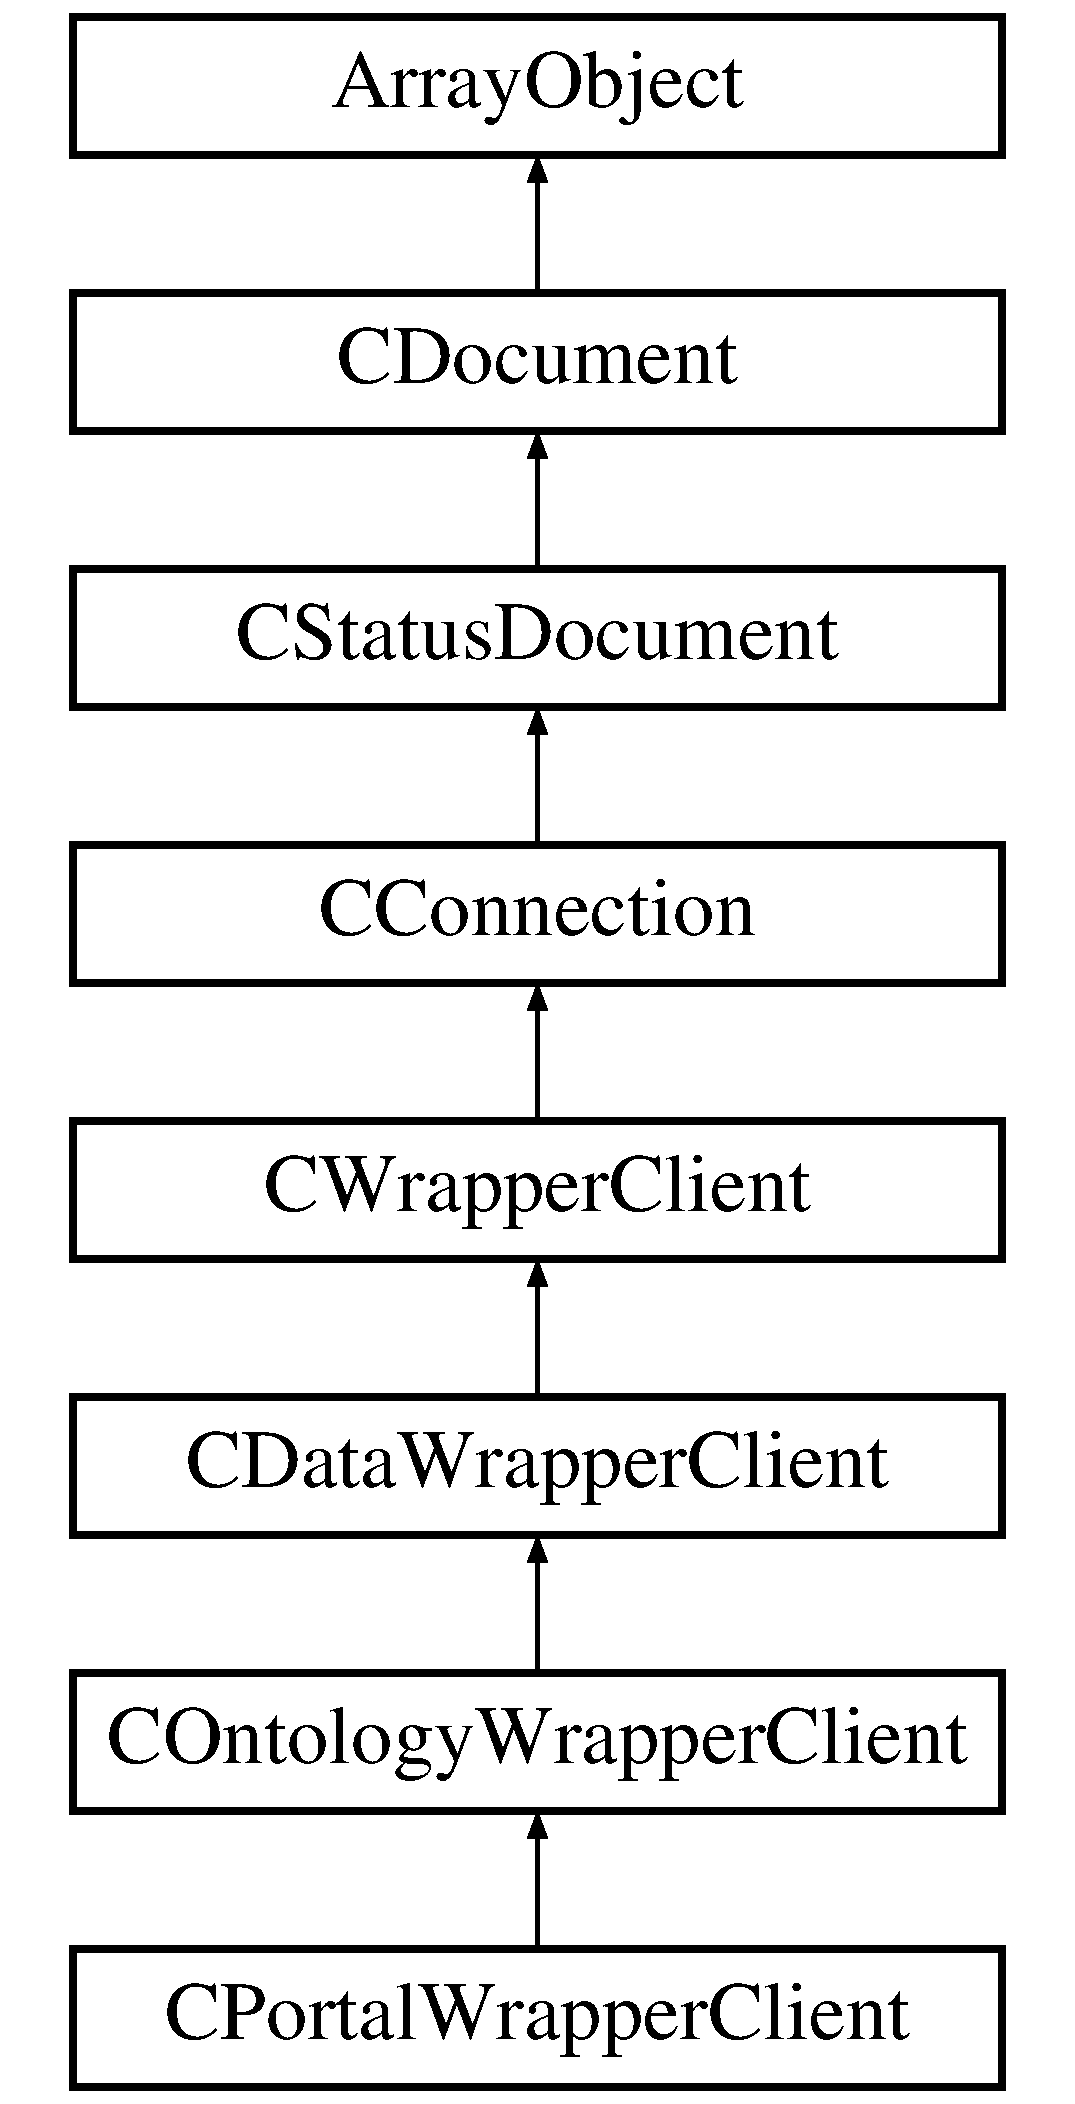
\includegraphics[height=8.000000cm]{class_c_wrapper_client}
\end{center}
\end{figure}
\subsection*{Public Member Functions}
\begin{DoxyCompactItemize}
\item 
\hyperlink{class_c_wrapper_client_ab59e31a65a939dc99630aaabebdb01cf}{\-\_\-\-\_\-to\-String} ()
\item 
\hyperlink{class_c_wrapper_client_ae378229fd57b051ddf0e0a7abf599641}{Operation} (\$the\-Value=N\-U\-L\-L, \$get\-Old=F\-A\-L\-S\-E)
\item 
\hyperlink{class_c_wrapper_client_aeea011893f53a7df495f23e199cbc28b}{Format} (\$the\-Value=N\-U\-L\-L, \$get\-Old=F\-A\-L\-S\-E)
\item 
\hyperlink{class_c_wrapper_client_ac87e4af5c32d735f192c8041e83b3ce3}{Stamp} (\$the\-Value=N\-U\-L\-L, \$get\-Old=F\-A\-L\-S\-E)
\item 
\hyperlink{class_c_wrapper_client_a844a2e677c1e0fb0855255cb02b86be4}{Log\-Request} (\$the\-Value=N\-U\-L\-L, \$get\-Old=F\-A\-L\-S\-E)
\item 
\hyperlink{class_c_wrapper_client_a2020117737285ff3c2c3f0fae01136ff}{Log\-Trace} (\$the\-Value=N\-U\-L\-L, \$get\-Old=F\-A\-L\-S\-E)
\item 
\hyperlink{class_c_wrapper_client_abf6475dc50f52a1f80b2eebc91fe4b95}{Execute} (\$the\-Mode= 'P\-O\-S\-T', \$do\-Encode=T\-R\-U\-E)
\item 
\hyperlink{class_c_wrapper_client_a8d444816f701541f165c112c9230fb97}{Dump} ()
\end{DoxyCompactItemize}
\subsection*{Static Public Member Functions}
\begin{DoxyCompactItemize}
\item 
static \hyperlink{class_c_wrapper_client_ac82b7d383afcfaa312f6db5eee1db4e2}{Request} (\$the\-Url, \$the\-Params=N\-U\-L\-L, \$the\-Mode= 'P\-O\-S\-T', \$the\-Format=k\-T\-Y\-P\-E\-\_\-\-J\-S\-O\-N)
\end{DoxyCompactItemize}
\subsection*{Protected Member Functions}
\begin{DoxyCompactItemize}
\item 
\hyperlink{class_c_wrapper_client_a829d4b5bcc5549e59913c6f83ea6afaa}{\-\_\-\-Ready} ()
\item 
\hyperlink{class_c_wrapper_client_ad2705e5b4a573bfb71ce7841c60b8c21}{\-\_\-\-Check\-Dependencies} (\$the\-Operation)
\item 
\hyperlink{class_c_wrapper_client_ae7294d66b5b54c1e9f033783fd2b009f}{\-\_\-\-Normalise\-Parameters} ()
\item 
\hyperlink{class_c_wrapper_client_a1b944a01fb65fc745461795766bd64ea}{\-\_\-\-Encode\-Parameters} (\&\$the\-Parameters, \$the\-Encoding)
\item 
\hyperlink{class_c_wrapper_client_a8ad42378b7abfeaaaa311e1b96a42a26}{\-\_\-\-Manage\-List\-Offset} (\$the\-Offset, \$the\-Value=N\-U\-L\-L, \$get\-Old=F\-A\-L\-S\-E)
\end{DoxyCompactItemize}
\subsection*{Additional Inherited Members}


\subsection{Member Function Documentation}
\hypertarget{class_c_wrapper_client_ab59e31a65a939dc99630aaabebdb01cf}{\index{C\-Wrapper\-Client@{C\-Wrapper\-Client}!\-\_\-\-\_\-to\-String@{\-\_\-\-\_\-to\-String}}
\index{\-\_\-\-\_\-to\-String@{\-\_\-\-\_\-to\-String}!CWrapperClient@{C\-Wrapper\-Client}}
\subsubsection[{\-\_\-\-\_\-to\-String}]{\setlength{\rightskip}{0pt plus 5cm}C\-Wrapper\-Client\-::\-\_\-\-\_\-to\-String (
\begin{DoxyParamCaption}
{}
\end{DoxyParamCaption}
)}}\label{class_c_wrapper_client_ab59e31a65a939dc99630aaabebdb01cf}
\subparagraph*{Return connection name}

This method should return the current client's name, in this class we return the client's U\-R\-L (\hyperlink{class_c_connection_a8ad981138c7b681c875da778ce4e391b}{Connection()}.

public \begin{DoxyReturn}{Returns}
string The client name. 
\end{DoxyReturn}
\hypertarget{class_c_wrapper_client_ad2705e5b4a573bfb71ce7841c60b8c21}{\index{C\-Wrapper\-Client@{C\-Wrapper\-Client}!\-\_\-\-Check\-Dependencies@{\-\_\-\-Check\-Dependencies}}
\index{\-\_\-\-Check\-Dependencies@{\-\_\-\-Check\-Dependencies}!CWrapperClient@{C\-Wrapper\-Client}}
\subsubsection[{\-\_\-\-Check\-Dependencies}]{\setlength{\rightskip}{0pt plus 5cm}C\-Wrapper\-Client\-::\-\_\-\-Check\-Dependencies (
\begin{DoxyParamCaption}
\item[{}]{\$the\-Operation}
\end{DoxyParamCaption}
)\hspace{0.3cm}{\ttfamily [protected]}}}\label{class_c_wrapper_client_ad2705e5b4a573bfb71ce7841c60b8c21}
Check operation dependencies.

This method can be used to assert whether the required parameters are present depending on the requested operation.


\begin{DoxyParams}[1]{Parameters}
string & {\em \$the\-Operation} & Requested operation.\\
\hline
\end{DoxyParams}
protected


\begin{DoxyExceptions}{Exceptions}
{\em Exception} & \\
\hline
\end{DoxyExceptions}
\hypertarget{class_c_wrapper_client_a1b944a01fb65fc745461795766bd64ea}{\index{C\-Wrapper\-Client@{C\-Wrapper\-Client}!\-\_\-\-Encode\-Parameters@{\-\_\-\-Encode\-Parameters}}
\index{\-\_\-\-Encode\-Parameters@{\-\_\-\-Encode\-Parameters}!CWrapperClient@{C\-Wrapper\-Client}}
\subsubsection[{\-\_\-\-Encode\-Parameters}]{\setlength{\rightskip}{0pt plus 5cm}C\-Wrapper\-Client\-::\-\_\-\-Encode\-Parameters (
\begin{DoxyParamCaption}
\item[{\&}]{\$the\-Parameters, }
\item[{}]{\$the\-Encoding}
\end{DoxyParamCaption}
)\hspace{0.3cm}{\ttfamily [protected]}}}\label{class_c_wrapper_client_a1b944a01fb65fc745461795766bd64ea}
Encode parameters.

This method can be used to encode parameters before they get sent to the service.

The method expects one parameter to be a reference to the list of parameter that will be sent and the other to be the format in which the parameters myst be encoded. This value is assumed to be an array.

If the provided encoding is not recognised by the method, the parameters will be left untouched; in derived classes you should first call the parent method and then handle the local parameters.


\begin{DoxyParams}[1]{Parameters}
reference & {\em \&\$the\-Parameters} & List of parameters. \\
\hline
string & {\em \$the\-Encoding} & Encoding code.\\
\hline
\end{DoxyParams}
protected \hypertarget{class_c_wrapper_client_a8ad42378b7abfeaaaa311e1b96a42a26}{\index{C\-Wrapper\-Client@{C\-Wrapper\-Client}!\-\_\-\-Manage\-List\-Offset@{\-\_\-\-Manage\-List\-Offset}}
\index{\-\_\-\-Manage\-List\-Offset@{\-\_\-\-Manage\-List\-Offset}!CWrapperClient@{C\-Wrapper\-Client}}
\subsubsection[{\-\_\-\-Manage\-List\-Offset}]{\setlength{\rightskip}{0pt plus 5cm}C\-Wrapper\-Client\-::\-\_\-\-Manage\-List\-Offset (
\begin{DoxyParamCaption}
\item[{}]{\$the\-Offset, }
\item[{}]{\$the\-Value = {\ttfamily NULL}, }
\item[{}]{\$get\-Old = {\ttfamily FALSE}}
\end{DoxyParamCaption}
)\hspace{0.3cm}{\ttfamily [protected]}}}\label{class_c_wrapper_client_a8ad42378b7abfeaaaa311e1b96a42a26}
Manage a list offset.

This method is similar to the \hyperlink{}{Manage\-Offset()} function, except that it is assumed that the offset must contain an array\-: if you provide an array as the value, the method will behave as \hyperlink{}{Manage\-Offset()}; if you provide a scalar, the method will convert it to a string and add it to the existing array if it doesn't exist already, or create a new list with it. It is not possible to retrieve or delete single elements of the list, only add.


\begin{DoxyParams}[1]{Parameters}
string & {\em \$the\-Offset} & Offset to be managed. \\
\hline
mixed & {\em \$the\-Value} & New value or operation. \\
\hline
boolean & {\em \$get\-Old} & T\-R\-U\-E get old value.\\
\hline
\end{DoxyParams}
protected \begin{DoxyReturn}{Returns}
array
\end{DoxyReturn}

\begin{DoxyExceptions}{Exceptions}
{\em Exception} & \\
\hline
\end{DoxyExceptions}
\hypertarget{class_c_wrapper_client_ae7294d66b5b54c1e9f033783fd2b009f}{\index{C\-Wrapper\-Client@{C\-Wrapper\-Client}!\-\_\-\-Normalise\-Parameters@{\-\_\-\-Normalise\-Parameters}}
\index{\-\_\-\-Normalise\-Parameters@{\-\_\-\-Normalise\-Parameters}!CWrapperClient@{C\-Wrapper\-Client}}
\subsubsection[{\-\_\-\-Normalise\-Parameters}]{\setlength{\rightskip}{0pt plus 5cm}C\-Wrapper\-Client\-::\-\_\-\-Normalise\-Parameters (
\begin{DoxyParamCaption}
{}
\end{DoxyParamCaption}
)\hspace{0.3cm}{\ttfamily [protected]}}}\label{class_c_wrapper_client_ae7294d66b5b54c1e9f033783fd2b009f}
Normalise parameters.

This method can be used to normalise parameters before they get encoded.

In this class we set the request time stamp if the current value is not an float.

In derived classes you should call first the parent method, then handle the local parameters.

protected \hypertarget{class_c_wrapper_client_a829d4b5bcc5549e59913c6f83ea6afaa}{\index{C\-Wrapper\-Client@{C\-Wrapper\-Client}!\-\_\-\-Ready@{\-\_\-\-Ready}}
\index{\-\_\-\-Ready@{\-\_\-\-Ready}!CWrapperClient@{C\-Wrapper\-Client}}
\subsubsection[{\-\_\-\-Ready}]{\setlength{\rightskip}{0pt plus 5cm}C\-Wrapper\-Client\-::\-\_\-\-Ready (
\begin{DoxyParamCaption}
{}
\end{DoxyParamCaption}
)\hspace{0.3cm}{\ttfamily [protected]}}}\label{class_c_wrapper_client_a829d4b5bcc5549e59913c6f83ea6afaa}
\subparagraph*{Determine if the object is ready}

In this class we tie the \hyperlink{class_c_status_document_a954dee06e219e0a0f2e7fa6edac56e28}{\-\_\-\-Is\-Inited()} status to the presence or absence of the \hyperlink{}{k\-A\-P\-I\-\_\-\-O\-P\-E\-R\-A\-T\-I\-O\-N} and \hyperlink{}{k\-A\-P\-I\-\_\-\-F\-O\-R\-M\-A\-T} parameters.

protected \begin{DoxyReturn}{Returns}
boolean {\ttfamily T\-R\-U\-E} means \hyperlink{}{.  \-\_\-\-Ready() }
\end{DoxyReturn}
\hypertarget{class_c_wrapper_client_a8d444816f701541f165c112c9230fb97}{\index{C\-Wrapper\-Client@{C\-Wrapper\-Client}!Dump@{Dump}}
\index{Dump@{Dump}!CWrapperClient@{C\-Wrapper\-Client}}
\subsubsection[{Dump}]{\setlength{\rightskip}{0pt plus 5cm}C\-Wrapper\-Client\-::\-Dump (
\begin{DoxyParamCaption}
{}
\end{DoxyParamCaption}
)}}\label{class_c_wrapper_client_a8d444816f701541f165c112c9230fb97}
Return the request dump.

This method can be used to retrieve the object as an array for debugging purposes.

public \begin{DoxyReturn}{Returns}
array 
\end{DoxyReturn}
\hypertarget{class_c_wrapper_client_abf6475dc50f52a1f80b2eebc91fe4b95}{\index{C\-Wrapper\-Client@{C\-Wrapper\-Client}!Execute@{Execute}}
\index{Execute@{Execute}!CWrapperClient@{C\-Wrapper\-Client}}
\subsubsection[{Execute}]{\setlength{\rightskip}{0pt plus 5cm}C\-Wrapper\-Client\-::\-Execute (
\begin{DoxyParamCaption}
\item[{}]{\$the\-Mode = {\ttfamily 'POST'}, }
\item[{}]{\$do\-Encode = {\ttfamily TRUE}}
\end{DoxyParamCaption}
)}}\label{class_c_wrapper_client_abf6475dc50f52a1f80b2eebc91fe4b95}
Send an H\-T\-T\-P request.

This method can be used to sent an {\itshape H\-T\-T\-P} request using the current contents of the object and return a response.

If the second parameter is {\ttfamily T\-R\-U\-E}, the response will be encoded, if {\ttfamily F\-A\-L\-S\-E}, the reqponse will be returned in its original encoding.


\begin{DoxyParams}[1]{Parameters}
string & {\em \$the\-Mode} & Request mode, P\-O\-S\-T or G\-E\-T \\
\hline
boolean & {\em \$do\-Encode} & T\-R\-U\-E means encode result.\\
\hline
\end{DoxyParams}
public \begin{DoxyReturn}{Returns}
mixed
\end{DoxyReturn}

\begin{DoxyExceptions}{Exceptions}
{\em \{@link} & \hyperlink{class_c_exception}{C\-Exception} \hyperlink{class_c_exception}{C\-Exception}\} \\
\hline
\end{DoxyExceptions}
\hypertarget{class_c_wrapper_client_aeea011893f53a7df495f23e199cbc28b}{\index{C\-Wrapper\-Client@{C\-Wrapper\-Client}!Format@{Format}}
\index{Format@{Format}!CWrapperClient@{C\-Wrapper\-Client}}
\subsubsection[{Format}]{\setlength{\rightskip}{0pt plus 5cm}C\-Wrapper\-Client\-::\-Format (
\begin{DoxyParamCaption}
\item[{}]{\$the\-Value = {\ttfamily NULL}, }
\item[{}]{\$get\-Old = {\ttfamily FALSE}}
\end{DoxyParamCaption}
)}}\label{class_c_wrapper_client_aeea011893f53a7df495f23e199cbc28b}
Manage format.

This method can be used to manage the \hyperlink{}{format} in which both the parameters are sent and the response is returned from the web-\/service. It accepts a parameter which represents either the web-\/service format code or this method operation, depending on its value\-:


\begin{DoxyItemize}
\item {\itshape N\-U\-L\-L}\-: Return the current value. 
\item {\itshape F\-A\-L\-S\-E}\-: Delete the current value. 
\item {\itshape other}\-: Set the value with the provided parameter. 
\end{DoxyItemize}

The second parameter is a boolean which if {\itshape T\-R\-U\-E} will return the {\itshape old} value when replacing values; if {\itshape F\-A\-L\-S\-E}, it will return the currently set value.

This method will check whether the provided format is supported, if this is not the case, it will raise an exception. Derived classes should first check their specific operations, if not matched, they should pass the parameter to the parent method. In this class we support the following operations\-:


\begin{DoxyItemize}
\item {\itshape \hyperlink{}{k\-T\-Y\-P\-E\-\_\-\-P\-H\-P}}\-: Parameters and response will be serialized. 
\item {\itshape \hyperlink{}{k\-T\-Y\-P\-E\-\_\-\-X\-M\-L}}\-: Parameters and response will be encoded in X\-M\-L. 
\item {\itshape \hyperlink{}{k\-T\-Y\-P\-E\-\_\-\-J\-S\-O\-N}}\-: Parameters and response will be encoded in J\-S\-O\-N. 
\item {\itshape \hyperlink{}{k\-T\-Y\-P\-E\-\_\-\-M\-E\-T\-A}}\-: This data type can be used to return service metadata, the \hyperlink{class_c_wrapper_client_abf6475dc50f52a1f80b2eebc91fe4b95}{request} will return headers metadata for troubleshooting, rather than the response from the web-\/service. 
\end{DoxyItemize}


\begin{DoxyParams}[1]{Parameters}
string & {\em \$the\-Value} & Value or operation. \\
\hline
boolean & {\em \$get\-Old} & T\-R\-U\-E get old value.\\
\hline
\end{DoxyParams}
public \begin{DoxyReturn}{Returns}
mixed
\end{DoxyReturn}

\begin{DoxyExceptions}{Exceptions}
{\em \{@link} & \hyperlink{class_c_exception}{C\-Exception} \hyperlink{class_c_exception}{C\-Exception}\}\\
\hline
\end{DoxyExceptions}
Manage\-Offset()

\begin{DoxySeeAlso}{See Also}
k\-A\-P\-I\-\_\-\-F\-O\-R\-M\-A\-T 

k\-A\-P\-I\-\_\-\-O\-P\-\_\-\-H\-E\-L\-P k\-A\-P\-I\-\_\-\-O\-P\-\_\-\-P\-I\-N\-G 
\end{DoxySeeAlso}
\hypertarget{class_c_wrapper_client_a844a2e677c1e0fb0855255cb02b86be4}{\index{C\-Wrapper\-Client@{C\-Wrapper\-Client}!Log\-Request@{Log\-Request}}
\index{Log\-Request@{Log\-Request}!CWrapperClient@{C\-Wrapper\-Client}}
\subsubsection[{Log\-Request}]{\setlength{\rightskip}{0pt plus 5cm}C\-Wrapper\-Client\-::\-Log\-Request (
\begin{DoxyParamCaption}
\item[{}]{\$the\-Value = {\ttfamily NULL}, }
\item[{}]{\$get\-Old = {\ttfamily FALSE}}
\end{DoxyParamCaption}
)}}\label{class_c_wrapper_client_a844a2e677c1e0fb0855255cb02b86be4}
Log request switch.

This method can be used to turn on or off the request section in the web-\/service response, the method accepts a single parameter that if resolves to {\itshape T\-R\-U\-E} it will turn on this option, if not it will turn it off.

The second parameter is a boolean which if {\itshape T\-R\-U\-E} will return the {\itshape old} value when replacing values; if {\itshape F\-A\-L\-S\-E}, it will return the currently set value.


\begin{DoxyParams}[1]{Parameters}
boolean & {\em \$the\-Value} & T\-R\-U\-E or F\-A\-L\-S\-E. \\
\hline
boolean & {\em \$get\-Old} & T\-R\-U\-E get old value.\\
\hline
\end{DoxyParams}
public \begin{DoxyReturn}{Returns}
mixed
\end{DoxyReturn}
Manage\-Offset()

\begin{DoxySeeAlso}{See Also}
k\-A\-P\-I\-\_\-\-L\-O\-G\-\_\-\-R\-E\-Q\-U\-E\-S\-T 
\end{DoxySeeAlso}
\hypertarget{class_c_wrapper_client_a2020117737285ff3c2c3f0fae01136ff}{\index{C\-Wrapper\-Client@{C\-Wrapper\-Client}!Log\-Trace@{Log\-Trace}}
\index{Log\-Trace@{Log\-Trace}!CWrapperClient@{C\-Wrapper\-Client}}
\subsubsection[{Log\-Trace}]{\setlength{\rightskip}{0pt plus 5cm}C\-Wrapper\-Client\-::\-Log\-Trace (
\begin{DoxyParamCaption}
\item[{}]{\$the\-Value = {\ttfamily NULL}, }
\item[{}]{\$get\-Old = {\ttfamily FALSE}}
\end{DoxyParamCaption}
)}}\label{class_c_wrapper_client_a2020117737285ff3c2c3f0fae01136ff}
Log trace switch.

This method can be used to turn on or off the trace in the event an exception is raised, the method accepts a single parameter that if resolves to {\itshape T\-R\-U\-E} it will turn on this option, if not it will turn it off.

The second parameter is a boolean which if {\itshape T\-R\-U\-E} will return the {\itshape old} value when replacing values; if {\itshape F\-A\-L\-S\-E}, it will return the currently set value.


\begin{DoxyParams}[1]{Parameters}
boolean & {\em \$the\-Value} & T\-R\-U\-E or F\-A\-L\-S\-E. \\
\hline
boolean & {\em \$get\-Old} & T\-R\-U\-E get old value.\\
\hline
\end{DoxyParams}
public \begin{DoxyReturn}{Returns}
mixed
\end{DoxyReturn}
Manage\-Offset()

\begin{DoxySeeAlso}{See Also}
k\-A\-P\-I\-\_\-\-L\-O\-G\-\_\-\-T\-R\-A\-C\-E 
\end{DoxySeeAlso}
\hypertarget{class_c_wrapper_client_ae378229fd57b051ddf0e0a7abf599641}{\index{C\-Wrapper\-Client@{C\-Wrapper\-Client}!Operation@{Operation}}
\index{Operation@{Operation}!CWrapperClient@{C\-Wrapper\-Client}}
\subsubsection[{Operation}]{\setlength{\rightskip}{0pt plus 5cm}C\-Wrapper\-Client\-::\-Operation (
\begin{DoxyParamCaption}
\item[{}]{\$the\-Value = {\ttfamily NULL}, }
\item[{}]{\$get\-Old = {\ttfamily FALSE}}
\end{DoxyParamCaption}
)}}\label{class_c_wrapper_client_ae378229fd57b051ddf0e0a7abf599641}
Manage operation.

This method can be used to manage the \hyperlink{}{operation}, it accepts a parameter which represents either the web-\/service operation code or this method operation, depending on its value\-:


\begin{DoxyItemize}
\item {\itshape N\-U\-L\-L}\-: Return the current value. 
\item {\itshape F\-A\-L\-S\-E}\-: Delete the current value. 
\item {\itshape other}\-: Set the value with the provided parameter. 
\end{DoxyItemize}

The second parameter is a boolean which if {\itshape T\-R\-U\-E} will return the {\itshape old} value when replacing values; if {\itshape F\-A\-L\-S\-E}, it will return the currently set value.

This method will check whether the provided operation is supported, if this is not the case, it will raise an exception. Derived classes should first check their specific operations, if not matched, they should pass the parameter to the parent method. In this class we support the following operations\-:


\begin{DoxyItemize}
\item {\itshape \hyperlink{}{k\-A\-P\-I\-\_\-\-O\-P\-\_\-\-H\-E\-L\-P}}\-: H\-E\-L\-P web-\/service operation, which returns the list of supported operations and options. 
\item {\itshape \hyperlink{}{k\-A\-P\-I\-\_\-\-O\-P\-\_\-\-P\-I\-N\-G}}\-: P\-I\-N\-G web-\/service operation, which returns a status response. 
\end{DoxyItemize}


\begin{DoxyParams}[1]{Parameters}
string & {\em \$the\-Value} & Value or operation. \\
\hline
boolean & {\em \$get\-Old} & T\-R\-U\-E get old value.\\
\hline
\end{DoxyParams}
public \begin{DoxyReturn}{Returns}
mixed
\end{DoxyReturn}

\begin{DoxyExceptions}{Exceptions}
{\em \{@link} & \hyperlink{class_c_exception}{C\-Exception}\}\\
\hline
\end{DoxyExceptions}
Manage\-Offset()

\begin{DoxySeeAlso}{See Also}
k\-A\-P\-I\-\_\-\-O\-P\-E\-R\-A\-T\-I\-O\-N 

k\-A\-P\-I\-\_\-\-O\-P\-\_\-\-H\-E\-L\-P k\-A\-P\-I\-\_\-\-O\-P\-\_\-\-P\-I\-N\-G 
\end{DoxySeeAlso}
\hypertarget{class_c_wrapper_client_ac82b7d383afcfaa312f6db5eee1db4e2}{\index{C\-Wrapper\-Client@{C\-Wrapper\-Client}!Request@{Request}}
\index{Request@{Request}!CWrapperClient@{C\-Wrapper\-Client}}
\subsubsection[{Request}]{\setlength{\rightskip}{0pt plus 5cm}static C\-Wrapper\-Client\-::\-Request (
\begin{DoxyParamCaption}
\item[{}]{\$the\-Url, }
\item[{}]{\$the\-Params = {\ttfamily NULL}, }
\item[{}]{\$the\-Mode = {\ttfamily 'POST'}, }
\item[{}]{\$the\-Format = {\ttfamily kTYPE\-\_\-JSON}}
\end{DoxyParamCaption}
)\hspace{0.3cm}{\ttfamily [static]}}}\label{class_c_wrapper_client_ac82b7d383afcfaa312f6db5eee1db4e2}
Send a H\-T\-T\-P request.

This method can be used to sent an {\itshape H\-T\-T\-P} request via {\itshape G\-E\-T} or {\itshape P\-O\-S\-T}.

The method accepts the following parameters\-:


\begin{DoxyItemize}
\item {\bfseries \$the\-Url}\-: The request U\-R\-L. 
\item {\bfseries \$the\-Params}\-: An array of key/value parameters for the request. 
\item {\bfseries \$the\-Mode}\-: The request mode\-: 
\begin{DoxyItemize}
\item {\ttfamily G\-E\-T}\-: G\-E\-T, default. 
\item {\ttfamily P\-O\-S\-T}\-: P\-O\-S\-T. 
\item {\itshape \hyperlink{}{k\-T\-Y\-P\-E\-\_\-\-M\-E\-T\-A}}\-: Metadata\-: if you provide this format, the method will return the metadata of the operation for troubleshooting purposes. 
\end{DoxyItemize}
\item {\bfseries \$the\-Format}\-: The request format\-: 
\begin{DoxyItemize}
\item {\ttfamily \hyperlink{}{k\-T\-Y\-P\-E\-\_\-\-P\-H\-P}}\-: P\-H\-P. 
\item {\ttfamily \hyperlink{}{k\-T\-Y\-P\-E\-\_\-\-J\-S\-O\-N}}\-: J\-S\-O\-N. 
\item {\ttfamily \hyperlink{}{k\-T\-Y\-P\-E\-\_\-\-M\-E\-T\-A}}\-: Metadata\-: the method will return the metadata of the operation for troubleshooting purposes. 
\item {\itshape other}\-: The service will return the data as it was received. 
\end{DoxyItemize}
\end{DoxyItemize}


\begin{DoxyParams}[1]{Parameters}
string & {\em \$the\-Url} & Request U\-R\-L. \\
\hline
mixed & {\em \$the\-Params} & Request parameters. \\
\hline
string & {\em \$the\-Mode} & Request mode. \\
\hline
string & {\em \$the\-Format} & Response format.\\
\hline
\end{DoxyParams}
\begin{DoxyReturn}{Returns}
mixed
\end{DoxyReturn}

\begin{DoxyExceptions}{Exceptions}
{\em \{@link} & \hyperlink{class_c_exception}{C\-Exception} \hyperlink{class_c_exception}{C\-Exception}\} \\
\hline
\end{DoxyExceptions}
\hypertarget{class_c_wrapper_client_ac87e4af5c32d735f192c8041e83b3ce3}{\index{C\-Wrapper\-Client@{C\-Wrapper\-Client}!Stamp@{Stamp}}
\index{Stamp@{Stamp}!CWrapperClient@{C\-Wrapper\-Client}}
\subsubsection[{Stamp}]{\setlength{\rightskip}{0pt plus 5cm}C\-Wrapper\-Client\-::\-Stamp (
\begin{DoxyParamCaption}
\item[{}]{\$the\-Value = {\ttfamily NULL}, }
\item[{}]{\$get\-Old = {\ttfamily FALSE}}
\end{DoxyParamCaption}
)}}\label{class_c_wrapper_client_ac87e4af5c32d735f192c8041e83b3ce3}
Time-\/stamp switch.

This method can be used to turn on or off the time-\/stamp section in the web-\/service response, the method accepts a single parameter that if resolves to {\itshape T\-R\-U\-E} it will turn on this option, if not it will turn it off.

The second parameter is a boolean which if {\itshape T\-R\-U\-E} will return the {\itshape old} value when replacing values; if {\itshape F\-A\-L\-S\-E}, it will return the currently set value.


\begin{DoxyParams}[1]{Parameters}
boolean & {\em \$the\-Value} & T\-R\-U\-E or F\-A\-L\-S\-E. \\
\hline
boolean & {\em \$get\-Old} & T\-R\-U\-E get old value.\\
\hline
\end{DoxyParams}
public \begin{DoxyReturn}{Returns}
mixed
\end{DoxyReturn}
Manage\-Offset()

\begin{DoxySeeAlso}{See Also}
k\-A\-P\-I\-\_\-\-S\-T\-A\-M\-P\-\_\-\-R\-E\-Q\-U\-E\-S\-T 
\end{DoxySeeAlso}


The documentation for this class was generated from the following file\-:\begin{DoxyCompactItemize}
\item 
/\-Library/\-Web\-Server/\-Library/\-P\-H\-P\-Wrapper/classes/C\-Wrapper\-Client.\-php\end{DoxyCompactItemize}

\addcontentsline{toc}{part}{Index}
\printindex
\end{document}
